\documentclass[11pt]{article}

% =====================================================================
%  ROOT 1 of 4 --- THE SUBMISSION MANUSCRIPT
%
%  Sibling documents:
%     sanctions_jet_appendix.tex   appendix reference document
%     sanctions_jet_notes.tex      staging / other information (not submitted)
%     sanctions_formal_supplement.tex  online formal-verification supplement
%
%  Two build modes (see scripts/Build-Paper.ps1):
%
%    SPLIT   (default)  the appendix is a separate PDF; cross-references
%                       into it are resolved through xr-hyper.
%    COMBINED           define \COMBINEDAPPENDIX and the appendix body is
%                       inlined, reproducing a single self-contained PDF
%                       with one unified bibliography:
%                         pdflatex "\def\COMBINEDAPPENDIX{}\documentclass[11pt]{article}

% =====================================================================
%  ROOT 1 of 4 --- THE SUBMISSION MANUSCRIPT
%
%  Sibling documents:
%     sanctions_jet_appendix.tex   appendix reference document
%     sanctions_jet_notes.tex      staging / other information (not submitted)
%     sanctions_formal_supplement.tex  online formal-verification supplement
%
%  Two build modes (see scripts/Build-Paper.ps1):
%
%    SPLIT   (default)  the appendix is a separate PDF; cross-references
%                       into it are resolved through xr-hyper.
%    COMBINED           define \COMBINEDAPPENDIX and the appendix body is
%                       inlined, reproducing a single self-contained PDF
%                       with one unified bibliography:
%                         pdflatex "\def\COMBINEDAPPENDIX{}\documentclass[11pt]{article}

% =====================================================================
%  ROOT 1 of 4 --- THE SUBMISSION MANUSCRIPT
%
%  Sibling documents:
%     sanctions_jet_appendix.tex   appendix reference document
%     sanctions_jet_notes.tex      staging / other information (not submitted)
%     sanctions_formal_supplement.tex  online formal-verification supplement
%
%  Two build modes (see scripts/Build-Paper.ps1):
%
%    SPLIT   (default)  the appendix is a separate PDF; cross-references
%                       into it are resolved through xr-hyper.
%    COMBINED           define \COMBINEDAPPENDIX and the appendix body is
%                       inlined, reproducing a single self-contained PDF
%                       with one unified bibliography:
%                         pdflatex "\def\COMBINEDAPPENDIX{}\documentclass[11pt]{article}

% =====================================================================
%  ROOT 1 of 4 --- THE SUBMISSION MANUSCRIPT
%
%  Sibling documents:
%     sanctions_jet_appendix.tex   appendix reference document
%     sanctions_jet_notes.tex      staging / other information (not submitted)
%     sanctions_formal_supplement.tex  online formal-verification supplement
%
%  Two build modes (see scripts/Build-Paper.ps1):
%
%    SPLIT   (default)  the appendix is a separate PDF; cross-references
%                       into it are resolved through xr-hyper.
%    COMBINED           define \COMBINEDAPPENDIX and the appendix body is
%                       inlined, reproducing a single self-contained PDF
%                       with one unified bibliography:
%                         pdflatex "\def\COMBINEDAPPENDIX{}\input{sanctions_jet_draft}"
%
%  New paper material does NOT get written here first.  It lands in an
%  appropriate file under note_sections/ and is promoted only on the author's decision
%  (project rule: CLAUDE.md Rule 21).
% =====================================================================

\input{sanctions_preamble}

% Resolve \Cref{app:...} etc. against the standalone appendix document.
% In COMBINED mode the appendix labels are defined locally, so importing
% them again would collide -- hence the guard.
\ifdefined\COMBINEDAPPENDIX\else
  \externaldocument[][nocite]{sanctions_jet_appendix}
\fi
\externaldocument[][nocite]{sanctions_formal_supplement}

\title{Political Entrenchment and the Persistence of Economic Sanctions}
% Corresponding author. Add ORCID iD before submission
% (Elsevier Editorial Manager requires both for the corresponding author).
\author{Xiaofeng Gong\thanks{Corresponding author. Department of
Economics, University of Connecticut, 365 Fairfield Way, Unit 1063,
Storrs, CT 06269-1063, USA. Email:
\texttt{xiaofeng.gong@uconn.edu}. Telephone: +1 857-384-2289.}
\and Yuechuan Zhao\thanks{National Academy of Economic Strategy, Chinese Academy of
Social Sciences, Beijing, China. Email: \texttt{zhaoyuechuan@ucass.edu.cn}.}
\and Chunping Zhong\thanks{National Academy of Economic Strategy, Chinese Academy of
Social Sciences, Beijing, China. Email: \texttt{cpzenith@163.com}.}}
\date{October 2026}

% @econ-contract master
% id: PAPER_MASTER_PLAN
% central_question: When sanctions move a political state that both governments value, can forward-looking incentives make sanctions persist where myopic ones would end them, and what does each government's foresight contribute?
% provisional_answer: At common non-discount primitives on the stated class, the myopic benchmark ends sanctions through relief while forward-looking governments sustain them under defiance with a positive long-run state; the Target's horizon decides accommodation against defiance and the Sender's horizon decides the compliance that relief buys or the sanction sustained under defiance; the defiance channel extends beyond the displayed profiles at stated quantifiers, and government incentives do not identify the social ranking.
% claim_ceiling: The myopic benchmark and the constructed forward-looking equilibrium, and the four cases in the discussion; existence inheritance under monotonicity hypotheses; a value bound in every top-selector equilibrium; uniqueness only in the nondecreasing-rule class; exactness only on the tight collapse class; welfare non-identification on the class by two representations, a sufficient condition for planner-optimal zero sanctions, and one representation under which full-defiance play is planner-optimal; no global uniqueness, complete classification, empirical or policy claim.
% principal_result_chain: Equilibrium environment and the myopic benchmark; the forward-looking equilibrium against it, with the Target's part and the Sender's wedge and same-policy dominance; lock-in; scope of the defiance channel (patience, security value, identification, certificates, exact collapse); welfare boundary; persistence is not hysteresis.
% reader_order: Abstract; Introduction (with literature); Model; Equilibrium and comparative statics; Welfare; Discussion; Conclusion; Appendix.
% build_order: Appendix intake; Model; Equilibrium and comparative statics; Welfare; Discussion; Introduction; Abstract; Conclusion.
% source_layout: SECTION_OWNED
% canonical_entrypoint: sanctions_jet_draft.tex
% status: HUMAN_CONFIRMED
% human_confirmed_at: 2026-10-01
% decision_ref: suggestions/2026-10-01-manuscript-rebuild/01_STRUCTURE_PROPOSAL.md#author-decisions-recorded
% confirmation_scope: Question, answer, claim ceiling, result chain, section order (D1), main-text propositions (D2, D5), headline pinning (D4).
% reopen_if: The question, the claim ceiling, the order of the principal moves, or the section layout changes.
% @end-econ-contract

\begin{document}

\maketitle

% @econ-contract paragraph
% id: ABSTRACT_SUMMARY
% role: State the model and its mechanism in the manner of Acemoglu and coauthors (N185), then the claims at their proved scope (the roles of the two governments' patience in the constructed equilibria, lock-in, welfare beyond the example economy, the Lean check), with no manuscript notation.
% amended_at: 2026-10-11 (fewer claims, lock-in added; the author: "cut down the number of the things on the abstract"); 2026-10-13 (argument plan: the problem first, "we show", "in one equilibrium", "beyond the example economy"; same claims); 2026-10-19 (coauthor wording review: wording of the coauthor's line-by-line revision applied where not wrong; sender/target in lower case; non-compliance for defiance; decision_ref: suggestions/2026-10-10-jet-submission/DECISIONS.md#coauthor-wording-review-2026-10-19); 2026-10-20 (N185 promoted: "We develop a dynamic model", the environment in plain sentences, the claims and their scope words unchanged, the Lean 4 sentence kept on the author's "maybe still add the usage of lean 4"; decision_ref: suggestions/2026-10-10-jet-submission/DECISIONS.md#acemoglu-comparison-and-model-exposition-2026-10-20)
% depends_on: PAPER_MASTER_PLAN
% handoff: The introduction.
% exact_ref: tex-label:sec:results
% support_status: VERIFIED
% status: PROPOSED
% @end-econ-contract
\begin{abstract}
\central{We develop a dynamic model in which economic sanctions shift the balance of
political power within the target country.} Each period the target chooses how far
to comply and the sender responds with sanctions. Sanctions raise political
entrenchment, the de facto power of target-side constituencies aligned with continued
confrontation, and both governments value this state. For a general class of economies, the
model provides conditions under which myopia makes sanctions unravel: the target
adjusts compliance just enough to induce sanction removal. When both governments are
forward-looking, the target maintains non-compliance and sanctions persist
indefinitely, even under complete information. The target's patience determines
whether relief or non-compliance prevails, while a forward-looking sender raises the
steady-state level of political entrenchment. Under stated conditions, a sufficiently
long temporary sanction shock locks in persistent sanctions. The game alone does not
pin down a welfare ranking. The core results are formally verified via machine-checked
proofs in Lean~4.
\end{abstract}

\medskip
\noindent\textbf{Keywords:} economic sanctions; persistence and
hysteresis; dynamic political economy; feedback Stackelberg equilibrium;
political entrenchment; path dependence.

\smallskip
\noindent\textbf{JEL classification:} C73; D72; F51; C61; D74.

% Elsevier Highlights are submitted separately and are intentionally
% omitted from the manuscript PDF.

% Section files follow the thin-root layout used by the reference project.
% @econ-contract include
% id: INCLUDE_INTRO
% file: main_sections/01_introduction.tex
% section_contract: INTRO_FRAME
% role: Pose the question and the experiment, state the three contributions at proved strength, and place them in the literature.
% question_answered: What question, how, and with what claim ceiling?
% required_inputs: All result sections (written last).
% output_handoff: Question, answer, ceiling and roadmap.
% claim_ceiling: The master plan's ceiling.
% status: HUMAN_CONFIRMED
% @end-econ-contract
\input{main_sections/01_introduction}
% @econ-contract include
% id: INCLUDE_MODEL
% file: main_sections/02_model.tex
% section_contract: MODEL_ENVIRONMENT
% role: Define the complete environment, the general class, the myopic benchmark with its one result, and the forward-looking equilibrium concept.
% question_answered: Who acts, in what order, with what information, objectives and restrictions?
% required_inputs: The accepted paper question.
% output_handoff: Objects, conditions, the benchmark and the solution concept for Section 3.
% claim_ceiling: Definitions and the myopic benchmark only.
% status: HUMAN_CONFIRMED
% @end-econ-contract
\input{main_sections/02_model}
% @econ-contract include
% id: INCLUDE_RESULTS
% file: main_sections/03_equilibrium_and_comparative_statics.tex
% section_contract: RESULTS_HORIZONS
% role: Compare forward-looking governments with the myopic benchmark, split the difference into the two governments' parts, and say how far the defiance channel reaches, each result at its own quantifier.
% question_answered: What does foresight add to the benchmark, what does each government's incentive contribute, and what extends beyond the constructions?
% required_inputs: MODEL_ENVIRONMENT.
% output_handoff: Proved horizon roles and their scope, for the welfare and discussion sections.
% claim_ceiling: As in the master plan; no global uniqueness or complete classification.
% status: HUMAN_CONFIRMED
% @end-econ-contract
\input{main_sections/03_equilibrium_and_comparative_statics}
% @econ-contract include
% id: INCLUDE_WELFARE
% file: main_sections/04_welfare.tex
% section_contract: WELFARE_BOUNDARY
% role: Separate the political ranking of the constructed regimes from a social ranking.
% question_answered: Do government incentives or a persistent equilibrium identify social welfare?
% required_inputs: RESULTS_HORIZONS.
% output_handoff: The welfare boundary for the discussion and the conclusion.
% claim_ceiling: Non-identification on the class; a sufficient planner condition; planner-optimal persistent play under one representation; one costly polity.
% status: HUMAN_CONFIRMED
% @end-econ-contract
\input{main_sections/04_welfare}
% @econ-contract include
% id: INCLUDE_DISCUSSION
% file: main_sections/05_discussion.tex
% section_contract: DISCUSSION_INTERPRETATION
% role: Solve the cases with one government forward-looking (the four-case theorem, moved from Section 3), then interpret persistence, relief, the case material and the limits of the results; no new results.
% question_answered: What do the results imply, and what do they not establish?
% required_inputs: RESULTS_HORIZONS, WELFARE_BOUNDARY, app:persistence.
% output_handoff: The interpretation boundary for the conclusion.
% claim_ceiling: The four-case theorem and summaries at stated scope; case material as motivation only.
% status: HUMAN_CONFIRMED
% @end-econ-contract
\input{main_sections/05_discussion}
% @econ-contract include
% id: INCLUDE_CONCLUSION
% file: main_sections/06_conclusion.tex
% section_contract: CONCLUSION_ANSWER
% role: Answer the question at its proved scope and state its limits.
% question_answered: What was established, and where does it stop?
% required_inputs: All result sections.
% output_handoff: None.
% claim_ceiling: The master plan's ceiling; no policy prescription.
% status: HUMAN_CONFIRMED
% @end-econ-contract
\input{main_sections/06_conclusion}
% @econ-contract include
% id: INCLUDE_DECLARATIONS
% file: main_sections/07_declarations.tex
% section_contract: DECLARATIONS_STATEMENTS
% role: Carry the required author declarations.
% question_answered: Competing interests, funding, contributions, AI use, data availability.
% required_inputs: Author records.
% output_handoff: None.
% claim_ceiling: Declarations only; no scientific claim.
% status: HUMAN_CONFIRMED
% @end-econ-contract
\input{main_sections/07_declarations}

\ifdefined\COMBINEDAPPENDIX
% @econ-contract include
% id: INCLUDE_APPENDIX_BODY
% file: sanctions_appendix_body.tex
% section_contract: APPENDIX_INDEX
% role: Inline the appendix in the combined build only; the split build cross-references the standalone appendix.
% question_answered: Where are the exact statements, proofs, constructed economies and the formalization map?
% required_inputs: All main sections.
% output_handoff: None.
% claim_ceiling: Exact statements and proofs of the results the main text states; no further claim.
% status: HUMAN_CONFIRMED
% @end-econ-contract
  \input{sanctions_appendix_body}
\fi

\bibliographystyle{econ-aea}
\bibliography{annote}

\end{document}
"
%
%  New paper material does NOT get written here first.  It lands in an
%  appropriate file under note_sections/ and is promoted only on the author's decision
%  (project rule: CLAUDE.md Rule 21).
% =====================================================================

% =====================================================================
%  SHARED PREAMBLE  --  sanctions_preamble.tex
%
%  Included by all four root documents:
%     sanctions_jet_draft.tex      (the submission manuscript)
%     sanctions_jet_appendix.tex   (the appendix reference document)
%     sanctions_jet_notes.tex      (the staging / other-information document)
%     sanctions_formal_supplement.tex (the online formal-verification supplement)
%
%  This file is NOT a document.  It carries only packages, theorem
%  environments, and macros, so the four roots cannot drift apart in
%  notation.  Anything document-specific (title, numbering scheme,
%  \externaldocument wiring) belongs in the root that needs it.
% =====================================================================

% ---------- Packages ----------
\usepackage[margin=1in]{geometry}
\usepackage{amsmath,amssymb,amsthm,mathtools}
\usepackage{enumitem}
% xr-hyper resolves \ref/\Cref/\eqref/\cite targets that live in a sibling
% document (main <-> appendix <-> notes).  It MUST be loaded before hyperref.
\usepackage{xr-hyper}
\usepackage[hidelinks]{hyperref}
\usepackage[nameinlink,capitalize]{cleveref}
\usepackage{aliascnt}
% thmtools removed 2026-08-07.  It was loaded but never used --- no
% \declaretheorem, no \listoftheorems, nothing but the \usepackage line ---
% and its current release (v0.76, 2023-05-04) patches \newtheorem in a way
% that breaks a shared-counter declaration such as
% \newtheorem{lemma}[theorem]{Lemma} under the 2026-06-01 LaTeX kernel
% ("Command \c@lemma already defined").  No newer thmtools is available.
% The theorem block below uses only amsthm, which handles it correctly.
\usepackage{booktabs}
\usepackage{array}
\usepackage{longtable}
\usepackage[expansion=false]{microtype}
\usepackage{graphicx}
\usepackage{caption}
\usepackage{natbib}
\usepackage{xurl}
\urlstyle{tt}
\usepackage{tikz}
\usetikzlibrary{arrows.meta,positioning,fit,backgrounds,calc,shapes.geometric}
\usepackage{pdflscape}

% ---------- Theorem Environments ----------
% Lemmas, propositions, corollaries, definitions and remarks share the theorem counter through
% alias counters (2026-10-11), so that cleveref names each by its own type: with a plain shared
% counter every \Cref of a proposition printed "Theorem". Their numbers expand to \thetheorem at
% print time, so the appendix's \numberwithin{theorem}{section} numbers them A.1, A.2, ... as before.
\theoremstyle{plain}
\newtheorem{theorem}{Theorem}
\newaliascnt{lemma}{theorem}
\newtheorem{lemma}[lemma]{Lemma}
\renewcommand{\thelemma}{\thetheorem}\renewcommand{\theHlemma}{\theHtheorem}
\crefname{lemma}{Lemma}{Lemmas}\Crefname{lemma}{Lemma}{Lemmas}
\newaliascnt{proposition}{theorem}
\newtheorem{proposition}[proposition]{Proposition}
\renewcommand{\theproposition}{\thetheorem}\renewcommand{\theHproposition}{\theHtheorem}
\crefname{proposition}{Proposition}{Propositions}\Crefname{proposition}{Proposition}{Propositions}
\newaliascnt{corollary}{theorem}
\newtheorem{corollary}[corollary]{Corollary}
\renewcommand{\thecorollary}{\thetheorem}\renewcommand{\theHcorollary}{\theHtheorem}
\crefname{corollary}{Corollary}{Corollaries}\Crefname{corollary}{Corollary}{Corollaries}

% Appendix sections must be cited as "Appendix C", never "Section C".
% This mattered little while the paper was one document; once the appendix
% is its own artefact, "Section C" points at a section the manuscript does
% not have.  The \crefalias that activates these lives immediately after
% \appendix in the shared sanctions_appendix_body.tex index, so it applies in BOTH the
% standalone appendix build and the COMBINED build.
\crefname{appendix}{Appendix}{Appendices}
\Crefname{appendix}{Appendix}{Appendices}
\crefname{subappendix}{Appendix}{Appendices}
\Crefname{subappendix}{Appendix}{Appendices}

\theoremstyle{definition}
\newtheorem{assumption}{Assumption}
\newaliascnt{definition}{theorem}
\newtheorem{definition}[definition]{Definition}
\renewcommand{\thedefinition}{\thetheorem}\renewcommand{\theHdefinition}{\theHtheorem}
\crefname{definition}{Definition}{Definitions}\Crefname{definition}{Definition}{Definitions}
\crefname{assumption}{Assumption}{Assumptions}
\Crefname{assumption}{Assumption}{Assumptions}

\theoremstyle{remark}
\newaliascnt{remark}{theorem}
\newtheorem{remark}[remark]{Remark}
\renewcommand{\theremark}{\thetheorem}\renewcommand{\theHremark}{\theHtheorem}
\crefname{remark}{Remark}{Remarks}\Crefname{remark}{Remark}{Remarks}

% ---------- Commands ----------
% Central sentence of a paragraph (2026-10-11): each paragraph's central sentence is wrapped in
% \central{...}. It prints as ordinary text; sanctions_jet_review.tex defines \centralmarks before
% loading the draft, which colours every central sentence for review.
\ifdefined\centralmarks
  \newcommand{\central}[1]{\textcolor{blue!55!black}{#1}}
\else
  \newcommand{\central}[1]{#1}
\fi
\newcommand{\R}{\mathbb{R}}
% Indicator. Was \mathbbm{1} from the bbm package; bbm lives in
% texlive-fonts-extra, which the CI TeX subset does not install, and the
% macro is used nowhere in the three documents. \mathbf carries the same
% glyph role with no extra package. Restore bbm here if the
% blackboard-bold indicator is ever wanted.
\newcommand{\1}{\mathbf{1}}
\newcommand{\Us}{U_S}
\newcommand{\Ut}{U_T}
\newcommand{\Vs}{V_S}
\newcommand{\Vt}{V_T}
\newcommand{\basin}{\mathcal{B}}
\newcommand{\sigDyn}{\sigma^{\mathrm{dyn}}}
\newcommand{\sigDynTop}{\sigma^{\mathrm{dyn}}}
\newcommand{\alphaM}{\alpha^{\mathrm{M}}}
\newcommand{\sigM}{\sigma^{\mathrm{M}}}
\newcommand{\F}{F}
\newcommand{\JSgroup}{\mathsf{J}_S}
\newcommand{\KSgroup}{\mathsf{K}_S}
\newcommand{\JTgroup}{\mathsf{J}_T}
\newcommand{\KTgroup}{\mathsf{K}_T}


% Resolve \Cref{app:...} etc. against the standalone appendix document.
% In COMBINED mode the appendix labels are defined locally, so importing
% them again would collide -- hence the guard.
\ifdefined\COMBINEDAPPENDIX\else
  \externaldocument[][nocite]{sanctions_jet_appendix}
\fi
\externaldocument[][nocite]{sanctions_formal_supplement}

\title{Political Entrenchment and the Persistence of Economic Sanctions}
% Corresponding author. Add ORCID iD before submission
% (Elsevier Editorial Manager requires both for the corresponding author).
\author{Xiaofeng Gong\thanks{Corresponding author. Department of
Economics, University of Connecticut, 365 Fairfield Way, Unit 1063,
Storrs, CT 06269-1063, USA. Email:
\texttt{xiaofeng.gong@uconn.edu}. Telephone: +1 857-384-2289.}
\and Yuechuan Zhao\thanks{National Academy of Economic Strategy, Chinese Academy of
Social Sciences, Beijing, China. Email: \texttt{zhaoyuechuan@ucass.edu.cn}.}
\and Chunping Zhong\thanks{National Academy of Economic Strategy, Chinese Academy of
Social Sciences, Beijing, China. Email: \texttt{cpzenith@163.com}.}}
\date{October 2026}

% @econ-contract master
% id: PAPER_MASTER_PLAN
% central_question: When sanctions move a political state that both governments value, can forward-looking incentives make sanctions persist where myopic ones would end them, and what does each government's foresight contribute?
% provisional_answer: At common non-discount primitives on the stated class, the myopic benchmark ends sanctions through relief while forward-looking governments sustain them under defiance with a positive long-run state; the Target's horizon decides accommodation against defiance and the Sender's horizon decides the compliance that relief buys or the sanction sustained under defiance; the defiance channel extends beyond the displayed profiles at stated quantifiers, and government incentives do not identify the social ranking.
% claim_ceiling: The myopic benchmark and the constructed forward-looking equilibrium, and the four cases in the discussion; existence inheritance under monotonicity hypotheses; a value bound in every top-selector equilibrium; uniqueness only in the nondecreasing-rule class; exactness only on the tight collapse class; welfare non-identification on the class by two representations, a sufficient condition for planner-optimal zero sanctions, and one representation under which full-defiance play is planner-optimal; no global uniqueness, complete classification, empirical or policy claim.
% principal_result_chain: Equilibrium environment and the myopic benchmark; the forward-looking equilibrium against it, with the Target's part and the Sender's wedge and same-policy dominance; lock-in; scope of the defiance channel (patience, security value, identification, certificates, exact collapse); welfare boundary; persistence is not hysteresis.
% reader_order: Abstract; Introduction (with literature); Model; Equilibrium and comparative statics; Welfare; Discussion; Conclusion; Appendix.
% build_order: Appendix intake; Model; Equilibrium and comparative statics; Welfare; Discussion; Introduction; Abstract; Conclusion.
% source_layout: SECTION_OWNED
% canonical_entrypoint: sanctions_jet_draft.tex
% status: HUMAN_CONFIRMED
% human_confirmed_at: 2026-10-01
% decision_ref: suggestions/2026-10-01-manuscript-rebuild/01_STRUCTURE_PROPOSAL.md#author-decisions-recorded
% confirmation_scope: Question, answer, claim ceiling, result chain, section order (D1), main-text propositions (D2, D5), headline pinning (D4).
% reopen_if: The question, the claim ceiling, the order of the principal moves, or the section layout changes.
% @end-econ-contract

\begin{document}

\maketitle

% @econ-contract paragraph
% id: ABSTRACT_SUMMARY
% role: State the model and its mechanism in the manner of Acemoglu and coauthors (N185), then the claims at their proved scope (the roles of the two governments' patience in the constructed equilibria, lock-in, welfare beyond the example economy, the Lean check), with no manuscript notation.
% amended_at: 2026-10-11 (fewer claims, lock-in added; the author: "cut down the number of the things on the abstract"); 2026-10-13 (argument plan: the problem first, "we show", "in one equilibrium", "beyond the example economy"; same claims); 2026-10-19 (coauthor wording review: wording of the coauthor's line-by-line revision applied where not wrong; sender/target in lower case; non-compliance for defiance; decision_ref: suggestions/2026-10-10-jet-submission/DECISIONS.md#coauthor-wording-review-2026-10-19); 2026-10-20 (N185 promoted: "We develop a dynamic model", the environment in plain sentences, the claims and their scope words unchanged, the Lean 4 sentence kept on the author's "maybe still add the usage of lean 4"; decision_ref: suggestions/2026-10-10-jet-submission/DECISIONS.md#acemoglu-comparison-and-model-exposition-2026-10-20)
% depends_on: PAPER_MASTER_PLAN
% handoff: The introduction.
% exact_ref: tex-label:sec:results
% support_status: VERIFIED
% status: PROPOSED
% @end-econ-contract
\begin{abstract}
\central{We develop a dynamic model in which economic sanctions shift the balance of
political power within the target country.} Each period the target chooses how far
to comply and the sender responds with sanctions. Sanctions raise political
entrenchment, the de facto power of target-side constituencies aligned with continued
confrontation, and both governments value this state. For a general class of economies, the
model provides conditions under which myopia makes sanctions unravel: the target
adjusts compliance just enough to induce sanction removal. When both governments are
forward-looking, the target maintains non-compliance and sanctions persist
indefinitely, even under complete information. The target's patience determines
whether relief or non-compliance prevails, while a forward-looking sender raises the
steady-state level of political entrenchment. Under stated conditions, a sufficiently
long temporary sanction shock locks in persistent sanctions. The game alone does not
pin down a welfare ranking. The core results are formally verified via machine-checked
proofs in Lean~4.
\end{abstract}

\medskip
\noindent\textbf{Keywords:} economic sanctions; persistence and
hysteresis; dynamic political economy; feedback Stackelberg equilibrium;
political entrenchment; path dependence.

\smallskip
\noindent\textbf{JEL classification:} C73; D72; F51; C61; D74.

% Elsevier Highlights are submitted separately and are intentionally
% omitted from the manuscript PDF.

% Section files follow the thin-root layout used by the reference project.
% @econ-contract include
% id: INCLUDE_INTRO
% file: main_sections/01_introduction.tex
% section_contract: INTRO_FRAME
% role: Pose the question and the experiment, state the three contributions at proved strength, and place them in the literature.
% question_answered: What question, how, and with what claim ceiling?
% required_inputs: All result sections (written last).
% output_handoff: Question, answer, ceiling and roadmap.
% claim_ceiling: The master plan's ceiling.
% status: HUMAN_CONFIRMED
% @end-econ-contract
% @econ-contract section
% id: INTRO_FRAME
% role: State the problem (common ground, the persistence fact, the standing complete-information objection, its consequence) and the question; give the paper's answer in three parts at their proved strength and levels of generality; state three contributions with their reasons (entrenchment through lock-in at every equilibrium of any economy that meets its conditions, entry under a temporary shock, low basins and persistence without hysteresis; what each government's patience decides, with the investment logic of defiance and a closed-form bound on the Sender's part; political persistence is not social welfare); answer the objections a referee will raise with proved results; give the roadmap; place the paper against the closest literature.
% question_answered: What question does the paper answer, how, and with what claim ceiling?
% required_inputs: RESULTS_HORIZONS, WELFARE_BOUNDARY, DISCUSSION_INTERPRETATION (written after them).
% output_handoff: The reader's question, answer, claim ceiling and roadmap.
% claim_ceiling: Exactly the master plan's ceiling; no manuscript notation by default.
% exclusions: The detailed literature (app:literature). The N134 sources enter as motivation only (promoted 2026-10-02 on the author's word). The conditions of lock-in and of persistence without hysteresis (Section 3.3).
% exact_ref: tex-label:sec:intro
% support_status: VERIFIED
% status: HUMAN_CONFIRMED
% human_confirmed_at: 2026-10-10
% decision_ref: suggestions/2026-10-10-terminology-rename/DECISIONS.md#contracts-reconfirmed
% confirmation_scope: Section role, claim ceiling, and the literature folded into the introduction (D1); first confirmed 2026-10-01 (suggestions/2026-10-01-manuscript-rebuild/01_STRUCTURE_PROPOSAL.md#author-decisions-recorded), reconfirmed 2026-10-10 after the Acemoglu--Wolitzky positioning (N180) and the terminology rename.
% reopen_if: The question, a principal result, or the literature positioning changes.
% amended_at: 2026-10-11 (lock-in as a numbered contribution; decision_ref: suggestions/2026-10-10-jet-submission/DECISIONS.md#lock-in-in-the-main-text); 2026-10-11 (no 'horizon'; no wording about what the paper is not; decision_ref: suggestions/2026-10-10-jet-submission/DECISIONS.md#plain-framing-2026-10-11); 2026-10-12 (three contributions around entrenchment; the dual-basin economy as the central illustration, after Lean round D; decision_ref: suggestions/2026-10-10-jet-submission/DECISIONS.md#framing-2026-10-12); 2026-10-13 (argument plan: problem before answer, one three-part answer with its levels of generality, the dual-basin economy said to lie outside the class (author's decision D2, reversing 'limits only in the conclusion' for this one clause), contributions with their warrants, a paragraph of objections and responses, the positioning paragraph moved into Section 1.1; decision_ref: suggestions/2026-10-10-jet-submission/exposition-2026-10-13/ARGUMENT_PLAN.md); 2026-10-15 (the dual-basin economy dropped from the main text for now, on the author's word; the first contribution rests on lock-in, and the 'outside the class' clause of D2 goes with the example); 2026-10-16 (layout decisions D1-D5: the answer and the contributions lead with foresight against the myopic benchmark, then lock-in, then welfare; decision_ref: suggestions/2026-10-10-jet-submission/DECISIONS.md#layout-myopic-benchmark-first-2026-10-16); 2026-10-16 (structure plan S1-S7 against the cited papers; decision_ref: suggestions/2026-10-10-jet-submission/DECISIONS.md#structure-plan-s1-s7-2026-10-16); 2026-10-17 (one contribution paragraph, directly before the roadmap, replaces the three that restated the answer; decision_ref: suggestions/2026-10-10-jet-submission/DECISIONS.md#one-contribution-paragraph-2026-10-17); 2026-10-19 (coauthor wording review: wording of the coauthor's line-by-line revision applied where not wrong; sender/target in lower case; non-compliance for defiance; decision_ref: suggestions/2026-10-10-jet-submission/DECISIONS.md#coauthor-wording-review-2026-10-19); 2026-10-20 (N185 opening paragraph; N184 de facto power sources; the comparison with Acemoglu and coauthors, INTRO_LIT_POWER_CONFLICT, and INTRO_LIT_HYSTERESIS split from it; decision_ref: suggestions/2026-10-10-jet-submission/DECISIONS.md#acemoglu-comparison-and-model-exposition-2026-10-20); 2026-10-20 (a footnote names the public repository; decision_ref: suggestions/2026-10-10-jet-submission/DECISIONS.md#public-repository-2026-10-20); 2026-10-20 (humanizer pass: dashes replaced by commas, parentheses or colons; plain wording; meaning unchanged; decision_ref: suggestions/2026-10-10-jet-submission/DECISIONS.md#humanizer-pass-2026-10-20)
% @end-econ-contract
\section{Introduction}
\label{sec:intro}

% @econ-contract paragraph
% id: INTRO_PUZZLE
% role: State the problem: sanctions as temporary coercion (common ground), the persistence fact the literature records (condition), the standing complete-information objection and what follows from it (consequence); then the question.
% depends_on: INTRO_FRAME
% handoff: The paper's answer in one sentence and the political state.
% exact_ref: bib:HalcoussisKaempferLowenberg2021#p=162
% source_role: bib:HalcoussisKaempferLowenberg2021#p=162 => Already-cited observation that prominent sanctions episodes have lasted for decades without fundamental change in the target government; motivation, not evidence for the mechanism; the episodes that sentence names (Cuba, Iran, North Korea) are named in the text (N185, 2026-10-20).
% exact_ref: bib:GAO2025RussiaSanctions#p=14
% source_role: bib:GAO2025RussiaSanctions#p=14 => The report's objectives for the U.S. measures on Russia (read 2026-10-02), worded as in Section 5 (DISC_SCOPE); an example of a sanctions regime's stated objectives, moved here from the deleted INTRO_SCOPE (2026-10-11); supports no model result.
% exact_ref: bib:Drezner2003#scope=paper
% source_role: bib:Drezner2003#scope=paper => Already-cited statement of the objection that imposed sanctions reflect failed bargaining or incomplete information; moved here from INTRO_CONFLICT_DYNAMICS as the paper's problem (argument plan, 2026-10-13); answered by the model, not supported by it.
% support_status: UNVERIFIED
% status: PROPOSED
% @end-econ-contract
\central{A striking feature of economic sanctions is how long some of them last.}
A sanctioning government restricts trade, financial, or diplomatic access to induce a
target government to change its behavior, and such measures are typically framed as
temporary instruments of coercion.\footnote{Stated objectives can be wider: those of the U.S. measures on
Russia are economic pressure, inhibition of the war effort, and accountability
\citep[p.~14]{GAO2025RussiaSanctions}.} Yet many prominent sanction episodes, for
example those against Cuba, Iran, and North Korea, have persisted for decades without
fundamental change in the target government
\citep[p.~162]{HalcoussisKaempferLowenberg2021}. This persistence is difficult to
reconcile with a standard result in sanction theory: under complete information,
targets concede at the threat stage, so actually imposed sanctions reflect either
bargaining failure or incomplete information \citep{Drezner2003}. If persistence
required such frictions, better information or more effective bargaining would end it.
Why, then, can sanctions persist between optimizing governments that know each other's
objectives, and how does each government's foresight shape the outcome?

% @econ-contract paragraph
% id: INTRO_EVIDENCE
% role: Give the paper's answer in one sentence (sanctions can strengthen the domestic constituencies that keep them in place), define the political state and the two stakes in words with the warrant for the Sender's stake, and give the Iran accounts with the stake each illustrates, as motivation and not as a test.
% depends_on: INTRO_PUZZLE
% handoff: The game.
% merged_from: INTRO_PUZZLE (its thesis and the definition of the political state, 2026-10-13)
% exact_ref: bib:BajoghliNasrSalehiIsfahaniVaez2024#pp=51-52
% source_role: bib:BajoghliNasrSalehiIsfahaniVaez2024#pp=51-52 => Interview accounts (read 2026-10-02) of Revolutionary Guard-linked enterprises gaining wealth under comprehensive sanctions while independent owners lost revenue and influence; motivation for a redistribution of influence, unquantified by the authors and not a test.
% exact_ref: bib:BajoghliNasrSalehiIsfahaniVaez2024#p=118
% source_role: bib:BajoghliNasrSalehiIsfahaniVaez2024#p=118 => The authors' statement (read 2026-10-02) that in the United States lifting sanctions on Iran carries a political cost while imposing them accrues political capital; motivation for Sender-side politics, not an identification of the Sender's stake.
% exact_ref: bib:AcemogluRobinson2008#p=268
% source_role: bib:AcemogluRobinson2008#p=268 => De facto power as influence not allocated by institutions (p. 268, read 2026-10-02, as in INTRO_LIT_POWER_CONFLICT); the sense of 'de facto power' at the first definition of political entrenchment (coauthor review, 2026-10-19), and the sources of such power, a group's wealth, weapons or ability to solve the collective action problem (N184, 2026-10-20); not support for a result.
% support_status: UNVERIFIED
% status: PROPOSED
% @end-econ-contract
\central{We focus on one domestic-political mechanism: sanctions can strengthen the
domestic constituencies that favor their continuation.} Government objectives
incorporate the political influence of interest groups, and sanctions alter this
influence by shifting a political state variable. This state, which we label
political entrenchment, is the de facto power
\citep[in the sense of][p.~268]{AcemogluRobinson2008} of target-side constituencies
whose interests are tied to continued confrontation. In their account, such power is not
allocated by formal institutions but derives from a group's wealth, weapons, or
ability to solve the collective action problem. It rises when sanctions exceed
its inherited level and erodes when sanctions fall below it. The target incumbent
values this state. We assume the sender's government also values it, modeling its
domestic ruling coalition as being sustained by a visibly entrenched adversary
(\Cref{sec:model:objectives}). Case studies of Iran sanctions illustrate both sides
of this mechanism. Qualitative evidence documents that enterprises tied to the
Revolutionary Guard accumulated wealth under comprehensive sanctions, while
independent business owners lost revenue and influence, so power shifted toward
constituencies aligned with confrontation; some within the ruling establishment
favored continuing the sanctions
\citep[pp.~51--52]{BajoghliNasrSalehiIsfahaniVaez2024}. In the sanctioning country,
lifting sanctions can carry a domestic political cost that imposing them does not
\citep[p.~118]{BajoghliNasrSalehiIsfahaniVaez2024}, a sender-side political dynamic
captured by the model's sender payoff function. These qualitative accounts motivate
our formal mechanism.

% @econ-contract paragraph
% id: INTRO_QUESTION
% role: Describe the game in words (timing, complete information, what each government weighs) and how the equilibria are obtained on a general class.
% depends_on: INTRO_EVIDENCE
% handoff: The answer.
% merged_from: INTRO_CONSTRUCTION (2026-10-13); the threshold special case moved to INTRO_CONTRIBUTION_ONE, and with it to INTRO_CONTRIBUTIONS (2026-10-17).
% exact_ref: tex-label:sec:model:class
% support_status: VERIFIED
% status: PROPOSED
% @end-econ-contract
\central{The two governments play a dynamic complete-information game.} In each
period, the target first chooses a level of compliance; the sender then observes
this choice and sets the intensity of sanctions. Information is complete and
monitoring is perfect, yet each government weighs both the current payoffs of its
actions and the future political entrenchment that its actions help shape. We
derive continuation values for both governments and verify that the sender's
response is optimal following every feasible compliance choice, both on and off
the equilibrium path, and that the target's choice is a best response at every
state, as required for a stationary feedback Stackelberg equilibrium. The general
results hold across a class of economies with general transition and payoff
functions; closed-form solutions for a quadratic--linear specification within the
class are reported in the Online Appendix.

% @econ-contract paragraph
% id: INTRO_PREVIEW
% role: Give the answer in three parts at their proved scope (foresight against the myopic benchmark, with the two governments' roles; lock-in under conditions on the equilibrium and the transition; welfare), then the levels of generality (reordered on the author's layout decisions, 2026-10-16). (2026-10-15: the dual-basin passage removed with the example, on the author's word.)
% depends_on: INTRO_QUESTION
% handoff: The related literature.
% merged_from: INTRO_EXPERIMENT (its result sentence, 2026-10-13)
% exact_ref: tex-label:prop:myopic-benchmark
% exact_ref: tex-label:thm:regime-separation
% exact_ref: tex-label:prop:lock-in
% exact_ref: tex-label:sec:welfare
% support_status: VERIFIED
% status: PROPOSED
% decision_ref: suggestions/2026-10-10-jet-submission/DECISIONS.md
% @end-econ-contract
\central{Our analysis delivers three core sets of results.} First, foresight
sustains sanction persistence. When both governments are myopic (they attach no
weight to future political entrenchment), the target accommodates: it adjusts
compliance just enough to induce the sender to halt sanctions, and the entrenchment
state erodes over time (\Cref{prop:myopic-benchmark}). When both governments are
forward-looking, the same economy supports an equilibrium where the target
maintains non-compliance, sanctions exceed the myopic sender's level and never end,
and the political state converges to a positive steady state
(\Cref{thm:regime-separation}). The target's patience determines whether relief or
non-compliance prevails; the sender's patience sets the compliance threshold for
relief or, under non-compliance, raises both sanction intensity and the steady-state
entrenchment level (\Cref{sec:results:wedge,sec:discussion:horizons}). Second,
sanctions exhibit lock-in effects. Under stated equilibrium and transition
conditions, once the political state enters a high basin (an interval of high
entrenchment), equilibrium play keeps it there and sanctions never decline. A
sufficiently long temporary sanction shock can move the state into this basin from
any initial condition (\Cref{prop:lock-in}). Third, the game alone does not pin down
a welfare ranking (\Cref{sec:welfare}). These results hold at varying levels of
generality. The benchmark comparison is derived from inequalities across model
primitives on the class, holding all primitives fixed except the discount factors;
lock-in holds at every equilibrium satisfying its conditions; and the welfare
results apply across the class, with an explicit interest-group polity and the
quadratic--linear family serving as illustrative examples.

\label{sec:literature}

% @econ-contract paragraph
% id: INTRO_POSITIONING
% moved: 2026-10-16, the related literature woven into the introduction without a heading (structure plan S1)
% role: Place the contribution against patient-conflict antecedents and antecedents with different discount factors, the source of the timing (Eaton and Engers without the threat stage, the author's word 2026-10-13) and the predecessor version, without claiming either is new; it states what the paper studies rather than a novelty claim, until a systematic antecedent search is done (author's word, 2026-10-03). Moved from before the roadmap into Section 1.1 (argument plan, 2026-10-13).
% depends_on: INTRO_PREVIEW
% handoff: The public-choice analysis of sanctions.
% exact_ref: bib:Eaton1992#scope=paper
% source_role: bib:Eaton1992#scope=paper => Already-cited antecedent relating each side's toughness to patience and sanction costs, with both parties discounting and no endogenous political state (the reading recorded in app:literature); the authors' stated source of the move order, without its threat stage (author's word, 2026-10-13); positions the contribution, does not support a result.
% exact_ref: bib:McBrideSkaperdas2009#scope=paper
% source_role: bib:McBrideSkaperdas2009#scope=paper => Already-cited working paper in which greater concern for future positions can favour conflict; positioning only.
% exact_ref: bib:GongZhong2025#scope=paper
% source_role: bib:GongZhong2025#scope=paper => The author-identified predecessor working paper; its acknowledged Target-patience and transition antecedents are retained.
% support_status: UNVERIFIED
% status: PROPOSED
% @end-econ-contract
\central{Patient conflict and differences in patience are established themes; we
study them in a target-first sanctions game in which the sender re-optimizes
each period and its sanctions move a political state that both incumbents
value.} That a longer shadow of the future can sustain conflict when today's
outcome shapes tomorrow's position is established in the theory of conflict
\citep{SkaperdasSyropoulos1996,GarfinkelSkaperdas2000,Powell2012,KraininWiseman2016},
typically under one common discount factor. Differences in patience also have
antecedents. \citet{Eaton1992} let the two sides of a sanctions game discount
differently, without an endogenous political state, and relate their toughness
to patience and sanction costs; our order of moves adapts their game without its
threat stage. \citet[Appendix~B]{McBrideSkaperdas2009} let a long-lived party
face one-period challengers. The earlier working paper \citet{GongZhong2025}
studies a target-only dynamic program, with target patience and the
partial-adjustment law as a leading example. A forward-looking sender with its
own discount factor is what allows the two governments' forward-looking
incentives to be separated.

% @econ-contract paragraph
% id: INTRO_LIT_PUBLIC_CHOICE
% role: Place the paper in the public-choice analysis of sanctions and say what is added.
% depends_on: INTRO_POSITIONING
% handoff: Endogenous political power and conflict.
% exact_ref: bib:Kaempfer1988#scope=paper
% source_role: bib:Kaempfer1988#scope=paper => Already-cited public-choice starting point; positioning only.
% support_status: UNVERIFIED
% status: PROPOSED
% @end-econ-contract
\central{Relative to the public-choice analysis of sanctions, the model makes the
political feedback dynamic and strategic.} Both governments' choices are derived
from continuation values over a political state that the sanction itself
moves. The public-choice starting point is \citet{Kaempfer1988}, who explain
sanctions through the political pressure and effectiveness of organized interest
groups. \citet{HalcoussisKaempferLowenberg2021} emphasize that sanctions may
retain domestic political functions after their direct leverage has diminished.
The model concerns how long sanctions last once imposed, and so complements
empirical work on duration and termination
\citep{BolksAlSowayel2000,AttiaGrauvogelVonSoest2020,AttiaGrauvogel2023}.

% @econ-contract paragraph
% id: INTRO_LIT_POWER_CONFLICT
% role: Compare the political state with the work of Acemoglu and coauthors on persistent political power (de facto power, its resource base, power shaped by those who hold it, persistent conflict) and state what the model adds: a stock moved by a foreign government's policy, the separate roles of two governments' foresight, lock-in by a temporary shock with welfare left open (the author's "Specifically compare with acemoglu", 2026-10-20); the Acemoglu--Wolitzky pointer and the standing objection under complete information moved to INTRO_CONFLICT_DYNAMICS (2026-10-11), hysteresis and lock-in to INTRO_LIT_HYSTERESIS (2026-10-20).
% depends_on: INTRO_LIT_PUBLIC_CHOICE
% handoff: Hysteresis and lock-in.
% exact_ref: bib:AcemogluRobinson2008#pp=268,272
% source_role: bib:AcemogluRobinson2008#pp=268,272 => De facto power as influence not allocated by institutions (p. 268), formally a per-period flow bought by the group while the persistent state is the regime (eq. 8, p. 272); read 2026-10-02; the stock/flow difference is stated.
% exact_ref: bib:AcemogluEgorovSonin2012#scope=abstract
% source_role: bib:AcemogluEgorovSonin2012#scope=abstract => "Current decisions determine the future distribution of political power" (read 2026-10-02); replaces AcemogluEgorovSonin2013, a two-period signalling model with no power state.
% exact_ref: bib:AcemogluRobinson2008#pp=279,287
% source_role: bib:AcemogluRobinson2008#pp=279,287 => Changes in de jure power 'can be partially or entirely offset by changes in de facto political power'; elites 'that are more forward-looking are more likely to dominate politics' (p. 287); investment in de facto power by the elite is 'socially costly' (p. 279); read 2026-10-20 (N184, N186); comparison, not support.
% exact_ref: bib:AcemogluJohnsonRobinson2005#scope=section-1.2
% source_role: bib:AcemogluJohnsonRobinson2005#scope=section-1.2 => A rich group's de facto power 'will tend to reproduce the initial relative wealth disparity'; 'shocks, including changes in technologies and the international environment, that modify the balance of (de facto) political power'; read 2026-10-20 (N186); comparison, not support.
% exact_ref: bib:AcemogluTicchiVindigni2010#p=664
% source_role: bib:AcemogluTicchiVindigni2010#p=664 => In weakly institutionalized polities a strong army 'opens the way for excessive influence or coups by the military', so civilian governments whose rents are largely unaffected by civil wars 'choose small and weak armies that are incapable of ending insurrections'; read 2026-10-20 (N186); comparison, not support.
% support_status: UNVERIFIED
% status: PROPOSED
% @end-econ-contract
\central{The model is closest to the work of Acemoglu and coauthors on persistent
political power, and it differs from that work in who moves the power state and in
what persists.} In \citet{AcemogluRobinson2008}, an elite buys de facto power anew
each period, and changes in it can partly or entirely offset changes in de jure power,
the power that formal institutions allocate, so that economic institutions persist
while political institutions change (pp.~268, 272, 287). In the framework of
\citet[Section~1.2]{AcemogluJohnsonRobinson2005}, a group's resources shape its de facto
power, which tends to reproduce the group's advantage unless shocks, including changes
in the international environment, modify the balance. In
\citet{AcemogluEgorovSonin2012,AcemogluEgorovSonin2015}, as in \citet{BaiLagunoff2011},
current decisions of those who hold power determine its future distribution. Domestic
politics can also keep a costly conflict going: in weakly institutionalized polities,
a civilian government whose rents a civil war leaves largely unaffected keeps its army
too small to end the war, because a strong army opens the way to military coups
\citep[p.~664]{AcemogluTicchiVindigni2010}. The model adds three things to this work.
(i)~The power state is a slow stock moved by a foreign government's policy: the
sender's sanctions, a change in the target's international environment, raise or erode
it, and what persists is that policy rather than a domestic institution. (ii)~Two
governments with separate discount factors act on the same state, so the roles of
foresight come apart. In \citet[p.~287]{AcemogluRobinson2008}, more forward-looking
elites are more likely to dominate politics; here a more patient target sustains
non-compliance whenever a less patient one does (\Cref{prop:patience-existence}),
while a forward-looking sender raises the steady-state level of political
entrenchment. (iii)~A temporary sanction shock can carry the state into a high basin
that equilibrium play does not leave (\Cref{prop:lock-in}), and the game does not
determine whether the resulting persistence is socially costly
(\Cref{prop:welfare-nonidentification}), whereas in
\citet[p.~279]{AcemogluRobinson2008} the elite's investment in de facto power is
socially costly.

% @econ-contract paragraph
% id: INTRO_LIT_HYSTERESIS
% role: Place persistence against hysteresis and lock-in models and point to the full positioning (split from INTRO_LIT_POWER_CONFLICT, 2026-10-20).
% depends_on: INTRO_LIT_POWER_CONFLICT
% handoff: Conflict under complete information.
% exact_ref: tex-label:app:literature
% source_role: tex-label:app:literature => The full positioning against hysteresis and lock-in models, to which the paragraph's footnote points (split from INTRO_LIT_POWER_CONFLICT, 2026-10-20).
% support_status: UNVERIFIED
% status: PROPOSED
% @end-econ-contract
\central{The model also relates to hysteresis and lock-in.} Relative to hysteresis
and lock-in models \citep{Dixit1989,Krugman1991,Arthur1989,HasslerEtAl2003},
persistence here is an equilibrium property of a game in which one government chooses
the instrument that moves the state, against the other's response.\footnote{The full
positioning, including the earlier working paper and the analytical methods, is
in \Cref{app:literature} of the Online Appendix.}

% @econ-contract paragraph
% id: INTRO_CONFLICT_DYNAMICS
% role: Say why sanctions can persist under complete information: place the political state against information-based and complete-information accounts of conflict dynamics, tie it to the objection stated in INTRO_PUZZLE without restating the four-case theorem (argument plan, 2026-10-13), and say what the state mechanism does at its stated scope.
% depends_on: INTRO_LIT_HYSTERESIS
% handoff: The verification statement and the roadmap.
% merged_from: INTRO_LIT_POWER_CONFLICT (part 2 only: its sentences 3 to 5; that block stays with part 1)
% exact_ref: bib:AcemogluWolitzky2014#scope=paper
% source_role: bib:AcemogluWolitzky2014#scope=paper => Spirals started by misperceptions end from inside as Bayesian players with limited memory come to treat a long spiral as uninformative about the opponent's type and experiment with cooperation (abstract; the reading recorded in app:literature); positioning only.
% exact_ref: bib:AcemogluWolitzkyMistrust#scope=sections-4-6
% source_role: bib:AcemogluWolitzkyMistrust#scope=sections-4-6 => Dates linked by persistent types (Section 4) or by threats to switch equilibria (Section 5.4); misperception and misunderstanding central to the onset, continuation and cessation of conflict (Section 6); positioning only.
% exact_ref: bib:SkaperdasSyropoulos1996#scope=paper
% source_role: bib:SkaperdasSyropoulos1996#scope=paper => Valuing the future sustains arming under complete information (the reading recorded in app:literature); positioning only.
% exact_ref: bib:Powell2012#scope=paper
% source_role: bib:Powell2012#scope=paper => Patient factions fight to forestall an adverse shift in power under complete information (the reading recorded in app:literature); positioning only.
% exact_ref: tex-label:sec:discussion:persistence
% exact_ref: bib:Drezner2003#scope=paper
% source_role: bib:Drezner2003#scope=paper => Already-cited statement of the objection that imposed sanctions reflect failed bargaining or incomplete information; stated in INTRO_PUZZLE and referred to here; answered by the model, not supported by it.
% exact_ref: bib:AcemogluWolitzkyMistrust#scope=sections-4-5
% source_role: bib:AcemogluWolitzkyMistrust#scope=sections-4-5 => Dates linked by persistent types (Section 4) or by threats to switch equilibria (Section 5.4); read 2026-10-02; positioning only.
% support_status: UNVERIFIED
% status: PROPOSED
% @end-econ-contract
\central{Sanctions can persist here under complete information because a
political state, which the sanctions themselves move, carries each government's
incentives from one date to the next.} Information-based accounts explain much
of the dynamics of conflict. In \citet{AcemogluWolitzky2014}, conflict spirals
end from inside: Bayesian players with limited memory come to treat a long
spiral as uninformative about the opponent's type and experiment with
cooperation. In the framework of \citet{AcemogluWolitzkyMistrust}, mistrust,
misperception and misunderstanding drive conflict, and dates are linked by a
belief about the opponent's type or a threat to switch equilibria. In
complete-information models, valuing the future can also sustain conflict
\citep{SkaperdasSyropoulos1996,Powell2012}. The political-state mechanism is of
that kind, with no belief to revise, and it is how the model answers the
objection of \citet{Drezner2003} stated at the outset. The same state can also
end a conflict: after a temporary suspension of sanctions, a resumed sanction rule that
stays at or below the state keeps de-escalation in place
(\Cref{sec:discussion:persistence}).
\Cref{sec:discussion:misperception} of the Online Appendix compares the two accounts
in detail.

% @econ-contract paragraph
% id: INTRO_VERIFICATION_ROADMAP
% role: State the verification status precisely (repair C8), in two sentences (argument plan, 2026-10-13); the roadmap follows in its own paragraph (INTRO_ROADMAP).
% depends_on: INTRO_CONFLICT_DYNAMICS
% handoff: The contributions.
% exact_ref: file:appendix_sections/07_formalization_map.tex#label=app:formalization
% source_role: file:appendix_sections/07_formalization_map.tex#label=app:formalization => The formal supplement's formalization map, which records the Lean declaration behind each statement; it establishes formal derivation, not economic correspondence.
% support_status: VERIFIED
% status: PROPOSED
% @end-econ-contract
\central{An Online Appendix and a formal supplement accompany the paper.} The
Online Appendix gives every proof and the precise statements of the results that
the main text gives in words. The formal supplement relates the core results to a
companion Lean~4 formalization, separately marks the analytic extensions that
rely on external existence results, and gives a separately reviewed map from the
formal statements to the paper's economic sentences.\footnote{The Lean~4 development, the
paper sources and the three documents are public at \url{https://github.com/qidaolake/political-entrenchment-sanctions-lean}.}

% @econ-contract paragraph
% id: INTRO_CONTRIBUTIONS
% role: State the paper's three contributions in one paragraph, directly before the roadmap (the author, 2026-10-17), keeping what the answer paragraph (INTRO_PREVIEW) does not say: the entrenchment condition and the investment logic of defiance, sufficient and not necessary; the Sender's foresight premium and defiance with a myopic Sender; the results beyond the constructed equilibria (a more patient Target, the threshold in the linear-quadratic special case, the minmax bound and uniqueness under the strong entrenchment condition, the participation result); lock-in at any equilibrium meeting its conditions, low basins, selection by the initial state and persistence without hysteresis; welfare non-identification and planner-optimal persistence.
% depends_on: INTRO_VERIFICATION_ROADMAP
% handoff: The roadmap.
% merged_from: INTRO_CONTRIBUTION_ONE; INTRO_PERSISTENCE; INTRO_CONTRIBUTION_THREE (2026-10-17)
% exact_ref: tex-label:sec:results:wedge
% exact_ref: tex-label:thm:four-cells
% exact_ref: tex-label:prop:patience-existence
% exact_ref: tex-label:prop:collapse-threshold
% exact_ref: tex-label:sec:results:security
% exact_ref: tex-label:sec:discussion:relief
% exact_ref: tex-label:sec:results:lockin
% exact_ref: tex-label:prop:welfare-nonidentification
% exact_ref: tex-label:prop:planner-efficient-persistence
% support_status: VERIFIED
% status: PROPOSED
% @end-econ-contract
\central{The paper makes three contributions.} First, it separates what each
government's foresight does to sanctions, holding every other primitive fixed. The
comparison rests on the entrenchment condition, under which non-compliance is an
investment: a sanction's pain today buys entrenchment worth at least as much, so a
forward-looking target accepts the sanction rather than pay to end it, while a
myopic one accommodates. The condition is sufficient for this, not necessary. A
forward-looking sender sanctions a non-compliant target more than a myopic one, by a
foresight premium with a closed-form lower bound (\Cref{sec:results:wedge}), and with a myopic
sender a forward-looking target still maintains non-compliance and sanctions stay positive
(\Cref{thm:four-cells}). Several results reach beyond the constructed equilibria: a
more patient target keeps a full-non-compliance equilibrium when the sender's response
does not fall with the state and a condition on primitives holds
(\Cref{prop:patience-existence}); in a linear--quadratic special case such an
equilibrium exists exactly from a threshold discount factor that the sender's
patience does not move (\Cref{prop:collapse-threshold}); under a stronger form of
the entrenchment condition every equilibrium gives the target at least its
pure-strategy minmax payoff, and on the class every equilibrium with a
non-decreasing sanction rule has full non-compliance (\Cref{sec:results:security}); and
no date-zero payment between the governments makes a temporary suspension of
sanctions acceptable to both (\Cref{sec:discussion:relief}). Second, it shows how
sanctions entrench themselves. Lock-in holds at any equilibrium of any economy that
meets explicit conditions; low sanctions can entrench themselves in the same way;
when one equilibrium has both a high and a low basin, the initial state selects
between them; and persistence need not mean hysteresis, since under further
conditions every start converges to the same long-run state
(\Cref{sec:results:lockin}). Third, it separates political persistence from social
welfare. Two interest-group representations that reproduce the governments'
payoffs, and so leave the equilibria unchanged, rank the forward-looking
equilibrium and the benchmark in opposite social orders
(\Cref{prop:welfare-nonidentification}). Under compliance neutrality some
representation makes the play of every full-non-compliance equilibrium socially optimal
(\Cref{prop:planner-efficient-persistence}), while in an explicit interest-group
polity in the tradition of \citet{Kaempfer1988} sanctions at one example economy
stay at their maximum although ending them would maximize aggregate welfare.
Evaluating welfare therefore requires group-level welfare primitives and an
explicit aggregation in addition to the equilibrium.

% @econ-contract paragraph
% id: INTRO_ROADMAP
% role: Give the roadmap, with the measurement requirements of the scope subsection (sec:discussion:scope).
% depends_on: INTRO_CONTRIBUTIONS
% handoff: The model (Section 2).
% split_from: INTRO_VERIFICATION_ROADMAP
% merged_from: INTRO_SCOPE
% merge_note: INTRO_SCOPE ("The paper is deliberately narrower than an assessment of sanctions.") was deleted on the author's word (2026-10-11); its sec:discussion:scope reference survives here, attached to the measurement requirements it stated, and its GAO2025RussiaSanctions citation survives in INTRO_PUZZLE.
% exact_ref: tex-label:sec:results:lockin
% exact_ref: tex-label:sec:discussion:scope
% support_status: NOT_APPLICABLE
% status: PROPOSED
% @end-econ-contract
\central{The rest of the paper sets out the model, the results on the class and
welfare.} \Cref{sec:model} defines the model and the example economies and solves
the myopic benchmark. \Cref{sec:results} compares forward-looking governments with
it, bounds the sender's part of the difference, and presents lock-in and the role
of the target's patience. \Cref{sec:welfare} separates the governments'
incentives from aggregate welfare. \Cref{sec:discussion} solves the cases in which
only one government looks forward, follows the path of the political state,
interprets the results and
states what empirical work would have to measure (\Cref{sec:discussion:scope}),
and \Cref{sec:conclusion} concludes.

% @econ-contract include
% id: INCLUDE_MODEL
% file: main_sections/02_model.tex
% section_contract: MODEL_ENVIRONMENT
% role: Define the complete environment, the general class, the myopic benchmark with its one result, and the forward-looking equilibrium concept.
% question_answered: Who acts, in what order, with what information, objectives and restrictions?
% required_inputs: The accepted paper question.
% output_handoff: Objects, conditions, the benchmark and the solution concept for Section 3.
% claim_ceiling: Definitions and the myopic benchmark only.
% status: HUMAN_CONFIRMED
% @end-econ-contract
% @econ-contract section
% id: MODEL_ENVIRONMENT
% role: Define the sequential game, the general class of transitions and objectives, the myopic benchmark with its one-period assumptions and prop:myopic-benchmark, the forward-looking equilibrium concept and the assumptions of the forward-looking results; define every symbol a later equation uses, and close with a notation table.
% question_answered: Who acts, in what order, with what information and objectives, under which restrictions, and what counts as an equilibrium?
% required_inputs: The accepted paper question and claim ceiling (PAPER_MASTER_PLAN).
% output_handoff: The objects, the admissible class with its theorem-specific conditions, and the solution concept used by Section 3.
% claim_ceiling: Definitions and maintained restrictions, and one result, the myopic benchmark (prop:myopic-benchmark); no other existence, uniqueness or comparative claim.
% exclusions: The basin assumptions A1-A3 and the conditional persistence machinery (appendix); the precise forms of the class's rate bounds and of the conditions other than the entrenchment condition (Online Appendix, panel A0); the conflict-structure reading (Section 5).
% exact_ref: tex-label:sec:model
% support_status: NOT_APPLICABLE
% status: HUMAN_CONFIRMED
% human_confirmed_at: 2026-10-01
% decision_ref: suggestions/2026-10-01-manuscript-rebuild/01_STRUCTURE_PROPOSAL.md#author-decisions-recorded
% confirmation_scope: Section role and claim ceiling only.
% reopen_if: Timing, information, the transition class, the payoff class or the solution concept changes.
% amended_at: 2026-10-13 (exposition: only the symbols that enter later equations are defined here; the other bounds and conditions are named in words with their precise forms in the Online Appendix; the dual-basin economy first among the examples; a notation table; decision_ref: suggestions/2026-10-10-jet-submission/DECISIONS.md#exposition-2026-10-13); 2026-10-15 (parametric examples only, the dual-basin economy and the numeric partial-adjustment example moved to the Online Appendix; the conditions as numbered Assumptions 1--10 marked with the results that use them; decision_ref: suggestions/2026-10-10-jet-submission/DECISIONS.md); 2026-10-16 (layout decisions D1-D5: the myopic benchmark with its one-period assumptions and prop:myopic-benchmark first, then forward-looking governments with their assumptions; the two conditions only the Sender-only case reads moved to the discussion; decision_ref: suggestions/2026-10-10-jet-submission/DECISIONS.md#layout-myopic-benchmark-first-2026-10-16); 2026-10-16 (the parametric examples, former Section 2.3, moved to the Online Appendix, sec:model:examples, on the author's word; decision_ref: suggestions/2026-10-10-jet-submission/DECISIONS.md#section-23-to-the-online-appendix-2026-10-16); 2026-10-16 (N183 promoted: a published precedent, or the contrast, at each assumption; Assumption 6 named Increasing differences after the cited works; decision_ref: suggestions/2026-10-10-jet-submission/DECISIONS.md#n183-promoted-literature-precedents-and-their-terms-2026-10-16); 2026-10-16 (compliance neutrality and the strong entrenchment condition leave the numbered assumptions and are stated with the results that read them; decision_ref: suggestions/2026-10-10-jet-submission/DECISIONS.md#four-conditions-leave-the-numbered-assumptions-2026-10-16); 2026-10-16 (structure plan S1-S7 against the cited papers; decision_ref: suggestions/2026-10-10-jet-submission/DECISIONS.md#structure-plan-s1-s7-2026-10-16); 2026-10-19 (coauthor wording review: wording of the coauthor's line-by-line revision applied where not wrong; sender/target in lower case; non-compliance for defiance; decision_ref: suggestions/2026-10-10-jet-submission/DECISIONS.md#coauthor-wording-review-2026-10-19); 2026-10-20 (the moves within a date as an enumerated list; (F1)-(F5) as a list; decision_ref: suggestions/2026-10-10-jet-submission/DECISIONS.md#acemoglu-comparison-and-model-exposition-2026-10-20); 2026-10-20 (subsection openings in the style of Acemoglu and coauthors, N187; the claims unchanged; decision_ref: suggestions/2026-10-10-jet-submission/DECISIONS.md#acemoglu-style-subsection-openings-2026-10-20); 2026-10-20 (plain-language reminders at the mathematics, N188; formal statements unchanged; decision_ref: suggestions/2026-10-10-jet-submission/DECISIONS.md#plain-language-reminders-at-the-mathematics-2026-10-20); 2026-10-20 (equation prose in the forms of Acemoglu and Robinson 2008, N189; decision_ref: suggestions/2026-10-10-jet-submission/DECISIONS.md#equation-prose-in-the-style-of-acemoglu-and-robinson-2026-10-20)
% @end-econ-contract
\section{Theoretical framework: sanctions and political entrenchment}
\label{sec:model}

\subsection{Timing, actions, and the political state}
\label{sec:model:timing}

% @econ-contract paragraph
% id: MODEL_TIMING
% role: State the timing as an enumerated sequence of the moves within a date (the author, 2026-10-20), observability and discounting, and what a myopic reading is; give the source of the order of moves (Eaton and Engers without the threat stage, the author's word 2026-10-13).
% depends_on: MODEL_ENVIRONMENT
% handoff: The state variable and its interpretation.
% exact_ref: bib:Eaton1992#scope=paper
% source_role: bib:Eaton1992#scope=paper => The authors' stated source of the move order (author's word, 2026-10-13): their sanctions game, in which the sender is committed between reviews (the reading recorded in app:literature), adapted without its threat stage; supports no result.
% support_status: UNVERIFIED
% status: PROPOSED
% @end-econ-contract
\central{Consider two governments, a target and a sender, that interact at dates $t=0,1,2,\ldots$
and move in sequence at each date.} Each date proceeds as follows.
\begin{enumerate}[label=(\arabic*)]
\item Both governments observe the political state $x_t\in[0,1]$, defined below.
\item The target chooses compliance $a_t\in[0,1]$.
\item The sender observes $a_t$ and chooses a sanction intensity $s_t\in[0,1]$.
\item Each government receives its per-period payoff, which depends on
$(x_t,a_t,s_t)$ (\Cref{sec:model:objectives}).
\item The state moves to $x_{t+1}$ by the law of motion~\eqref{eq:transition} below.
\end{enumerate}
The order adapts the sanctions game of \citet{Eaton1992} without its threat stage:
the sender announces nothing in advance and chooses its sanction after observing
compliance. The target therefore knows that its choice triggers the sender's response
and, in the economies studied here, that less compliance makes the sender want to
sanction more (\Cref{sec:model:objectives}). A period is one such review of
compliance, and every result uses this order. Actions and the state are observed by
both, and information is complete. The target and the sender discount their own
payoffs at $\beta_T,\beta_S\in[0,1)$. A government is \emph{myopic} when its discount
factor is zero and \emph{forward-looking} when it is positive.

% @econ-contract paragraph
% id: MODEL_STATE
% role: Say what the political state measures and how sanctions move it.
% depends_on: MODEL_TIMING
% handoff: The objectives.
% exact_ref: bib:Curtat1996#p=185
% source_role: bib:Curtat1996#p=185 => Monotonicity assumption of supermodular stochastic games (transition stochastically increasing in the state and actions); (F2)-(F3) are its deterministic counterpart (N183, 2026-10-16).
% exact_ref: bib:Amir2002#p=43
% source_role: bib:Amir2002#p=43 => Assumption (A7), higher states and actions lead to higher states, the stochastic form of (F2)-(F3) (N183).
% exact_ref: bib:AcemogluRobinson2008#p=278
% source_role: bib:AcemogluRobinson2008#p=278 => State dependence of political power (democracy more likely to follow democracy), read as the discrete-state precedent of (F2) (N183).
% exact_ref: bib:Kaempfer1988#p=791
% source_role: bib:Kaempfer1988#p=791 => The rally-around-the-flag effect by which sanctions can raise the regime supporters political effort, the precedent of (F3) (N183).
% support_status: VERIFIED
% status: PROPOSED
% @end-econ-contract
\central{The state $x_t$ is the de facto political power of the target's
isolationist and anti-concession constituencies, whose position is tied to
continued confrontation, and sanctions move it.} A sanction above the inherited
state raises it, and one below erodes it. Its law of motion is a reduced form
for how that power evolves. The law is
\begin{equation}
x_{t+1}=\F(x_t,s_t),
\label{eq:transition}
\end{equation}
where $\F\colon[0,1]^2\to[0,1]$ satisfies the following conditions throughout.
\begin{enumerate}[label=\textup{(F\arabic*)}]
\item $\F$ is continuous.
\item $\F$ is non-decreasing in the current state, so power persists.
\item $\F$ is non-decreasing in the sanction.
\item $\F(x,x)=x$ for every $x$: a sanction equal to the current state reproduces it.
\item For every $x,s\in[0,1]$, the state moves strictly toward the current sanction,
\[
s<x\ \Longrightarrow\ \F(x,s)<x,
\qquad
x<s\ \Longrightarrow\ x<\F(x,s).
\]
\end{enumerate}
With \textup{(F2)} and \textup{(F4)}, \textup{(F5)} rules out overshooting,
\[
s<x\ \Longrightarrow\ s\leq\F(x,s)<x,
\qquad
x<s\ \Longrightarrow\ x<\F(x,s)\leq s,
\]
so zero sanctions strictly erode every positive state, $\F(x,0)<x$ for
$x\in(0,1]$, and full sanctions strictly raise every state below one,
$x<\F(x,1)$ for $x\in[0,1)$. Comparing state and sanction is a normalization
within the model. Monotonicity of the law of motion in the state and in the sanction,
\textup{(F2)}--\textup{(F3)}, is the deterministic counterpart of the assumption,
standard in stochastic games, that higher states and actions lead to higher states
(\citealp[p.~185]{Curtat1996}; \citealp[p.~43]{Amir2002}). \textup{(F2)} is the state
dependence of political power of \citet[p.~278]{AcemogluRobinson2008} in a
continuous state, and \textup{(F3)} the rally effect by which a sanction can raise
the political effort of the target regime's supporters \citep[p.~791]{Kaempfer1988}. An interval of states from a threshold up to $1$ is a
\emph{high basin}, and one from $0$ up to a threshold a \emph{low basin}; the
results ask when equilibrium play keeps the state in such an interval.

\subsection{Objectives and the political stakes}
\label{sec:model:class}
\label{sec:model:objectives}

% @econ-contract paragraph
% id: MODEL_CLASS_PAYOFFS
% role: Define the payoffs and values, say that they are government objectives, and define full defiance and relief; one footnote gives where the precise forms of the bounds are.
% depends_on: MODEL_STATE
% handoff: The general class and the bounds that enter later equations.
% exact_ref: tex-label:app:proofs:placable
% support_status: VERIFIED
% status: PROPOSED
% @end-econ-contract
\central{We next turn to the governments' objectives: each government's per-period payoff depends
on the political state, the target's compliance and the sanction.}\footnote{The Online Appendix lists
every bound of the class in the form the proofs use (panel~A0 of
\Cref{app:proofs:placable}) and gives the closed forms of the derived constants
(\Cref{app:closedforms}).} Write $\Ut,\Us\colon[0,1]^3\to\R$ for the target's
and the sender's per-period payoffs in $(x,a,s)$, and $\Vt,\Vs$ for their
continuation values, which are bounded continuous functions of the state. The
payoffs are continuous. They are government objectives: they weight the
interest groups each government answers to, so they can differ from national
welfare (\Cref{sec:welfare}). A \emph{target policy} $\alpha$ gives compliance
as a function of the state. \emph{Full non-compliance} means $a=0$, and the
\emph{full-non-compliance policy} $\alpha\equiv0$ chooses it at every state; an
equilibrium (\Cref{sec:model:equilibrium}) with this policy is a
\emph{full-non-compliance equilibrium}. \emph{Full compliance} means $a=1$, and the
\emph{full sanction} $s=1$. \emph{Relief} means $s=0$, and \emph{permanent
relief} means $s=0$ at every date. The target
\emph{accommodates} when its compliance brings the sanction to zero.

% @econ-contract paragraph
% id: MODEL_CLASS_TRANSITION
% role: Say where the results use no functional form, and define the bounds that enter the main text's equations (state and sanction slopes of the transition, the Sender's stake and cost curvature, the Target's stake and pain).
% depends_on: MODEL_CLASS_PAYOFFS
% handoff: The economic content of the two state stakes.
% exact_ref: tex-label:app:proofs:placable
% exact_ref: bib:DorussenMo2001#p=407
% source_role: bib:DorussenMo2001#p=407 => The kappa parameter by which rent-seeking helps the target government decrease the costs of sanctions, a fixed-parameter version of entrenchment softening a sanction (N183).
% support_status: VERIFIED
% status: PROPOSED
% merged_from: MODEL_TRANSITION_GENERALITY
% @end-econ-contract
\central{The results use no functional form for the transition or for either
payoff.} They hold on a \emph{general class} of
economies defined by \textup{(F1)--(F5)} and by bounds on the slopes and
curvature of the transition and on the rates of the payoffs. No derivative is
assumed: each slope bound applies to every chord. The next state rises with the
current state and with the sanction, the latter at a rate bounded away from zero.
Both payoffs rise with the state at rates bounded away from zero, the target's
the more so the heavier the sanction, because entrenchment softens a sanction's
pain. A fixed version of this property is the parameter by which rent-seeking helps a
target government decrease the costs of sanctions in \citet[p.~407]{DorussenMo2001}. The curvature of the sender's cost of sanctioning and the pain of a
sanction to the target are bounded. The main text states these bounds in words
where a result uses them; their symbols and precise forms are in
\Cref{sec:moved-main-2026-10-13:conditions} of the Online Appendix. The paper's
parametric examples, a quadratic--linear family of payoffs and a partial-adjustment
law of motion, are in \Cref{sec:model:examples} of the Online Appendix.

% @econ-contract paragraph
% id: MODEL_STAKES
% role: State the two positive state stakes as the maintained political-incentive region, and whose valuations they are.
% depends_on: MODEL_CLASS_TRANSITION
% handoff: Compliance incentives and compliance neutrality.
% exact_ref: bib:Kaempfer1988#scope=paper
% source_role: bib:Kaempfer1988#scope=paper => Sender-side interest-group logic that the positive Sender stake restates as a continuation value; it does not establish the sign of any coefficient here.
% exact_ref: bib:BajoghliNasrSalehiIsfahaniVaez2024#p=118
% source_role: bib:BajoghliNasrSalehiIsfahaniVaez2024#p=118 => The authors' statement (read 2026-10-02) that in the United States lifting sanctions on Iran carries a political cost while imposing them accrues political capital; motivation for the Sender's stake (argument plan, 2026-10-13), not an identification of it.
% note: 2026-10-13 the response to the Sender-stake objection and the three distinct Sender-side features added (argument plan item 4).
% exact_ref: bib:DorussenMo2001#p=403
% source_role: bib:DorussenMo2001#p=403 => Audience costs make the sender prefer to remain with sanctions for domestic reasons while the target refuses to yield, and make sanctions cheaper for the sender the more extreme the target policy: a formal Sender-side precedent for the stake and for the state-sanction complementarity (N183).
% exact_ref: bib:AcemogluRobinson2008#p=268
% source_role: bib:AcemogluRobinson2008#p=268 => The elite invest in de facto power for the returns from controlling politics, the precedent of the Target incumbent stake (N183).
% support_status: UNVERIFIED
% status: PROPOSED
% @end-econ-contract
\central{The positive lower bounds on the two payoffs' state rates give both
incumbents a direct stake in the state.} The sender's stake is the substantive
assumption, and a reader may doubt that a sender gains from its adversary's
entrenchment. The sender's own coalition is modeled as sustained by a visibly
entrenched adversary, so the constituency the sanction strengthens abroad keeps
the sanction popular at home. The assumption restates the sender-side
interest-group logic of \citet{Kaempfer1988} as a continuation value. Sender-side politics of this kind are
documented: in the case of Iran,
lifting sanctions can carry a domestic political cost in the sanctioning country
that imposing them does not \citep[p.~118]{BajoghliNasrSalehiIsfahaniVaez2024}.
In a formal model of ending sanctions, audience costs lead the sender to prefer to
remain with sanctions for domestic reasons as long as the target refuses to yield
\citep[p.~403]{DorussenMo2001}.
Three sender-side features are distinct. The bound on its state rate is a
stake in the state itself. A state--sanction complementarity, where present,
makes the return to sanctioning rise with the state, as a state--sanction cross
term in the sender's payoff does; the audience-cost term of \citet{DorussenMo2001} is
one, under which sanctions cost the sender less the more extreme the target's
policy. And in the class the sender's one-period marginal
return to a first unit of sanction against a non-compliant target is positive at every
state, so its myopic best response sanctions a non-compliant target everywhere, and so
does its forward-looking response whenever its continuation value does not fall
with the state. Likewise the bound on the target's state rate describes the
target incumbent's valuation of the organized
influence the state measures, as the elite of \citet[p.~268]{AcemogluRobinson2008}
invest in de facto power for the returns from controlling politics. An explicit interest-group polity, with two groups
in each country, derives both stakes from a within-period political contest
(\Cref{sec:welfare}).

% @econ-contract paragraph
% id: MODEL_COMPLIANCE_NEUTRALITY
% role: Explain why compliance is costly at a fixed sanction, what pays for it, the compliance neutrality that relief results read, and the floor sanction and Target slope the entrenchment condition uses.
% depends_on: MODEL_STAKES
% handoff: The example economies.
% exact_ref: bib:Marinov2005#p=567
% source_role: bib:Marinov2005#p=567 => That concessions are costly is a central notion in the literature on economic pressure (quoted); the same page says the sender government cares about policy concessions, the coercion-model contrast with compliance neutrality (N183).
% exact_ref: bib:Eaton1992#p=903
% source_role: bib:Eaton1992#p=903 => The target utility decreases in its compliance action at given sanctions, the same restriction; the sender utility increases in it, the contrast with compliance neutrality (N183).
% exact_ref: bib:Kaempfer1988#scope=eqs-1-1prime
% source_role: bib:Kaempfer1988#scope=eqs-1-1prime => Sanctioning-country utilities defined over the sanction and its domestic incidence, not the target policy: the public-choice view that compliance neutrality follows (N183).
% exact_ref: bib:Tsebelis1990#scope=Assumptions-2-4
% source_role: bib:Tsebelis1990#scope=Assumptions-2-4 => The sender prefers to sanction a violation and not to sanction compliance, the binary form of a positive substitution rate (N183).
% support_status: VERIFIED
% status: PROPOSED
% @end-econ-contract
\central{Unlike the state, compliance pays the target only through the
sender's response.} It is costly at a fixed sanction, and it lowers the sender's
marginal return to sanctioning: compliance and the sanction are substitutes in the
sender's payoff, which has decreasing differences in them, at a rate we call the
\emph{substitution rate}. That concessions are costly to
the target is `a central notion in the literature on economic pressure'
(\citealp[p.~567]{Marinov2005}; see also \citealp[p.~903]{Eaton1992}), and the sender of
\citet[Assumptions~2 and~4]{Tsebelis1990} prefers to sanction a violation and not to
sanction compliance, the binary form of a positive substitution rate.
\emph{Compliance neutrality},
\begin{equation}
\Us(x,a,0)=\Us(x,0,0),
\label{eq:zero-sanction-neutrality}
\end{equation}
says that compliance is payoff-irrelevant to the sender at a zero sanction:
compliance matters to the sender only through its decision to sanction. It is not
one of the paper's assumptions; the three results that construct relief state it
(the relief side of \Cref{sec:results:patience}, \Cref{prop:planner-efficient-persistence}
and the sender-only case of \Cref{sec:discussion:horizons}). Along relief the
sanction is zero, so the sender's value can be computed before the target's
compliance is known; the positive results about non-compliance hold without it. Most coercion models let the sender value
compliance directly (\citealp[p.~903]{Eaton1992}; \citealp[p.~567]{Marinov2005});
compliance neutrality follows instead the public-choice view of
\citet[eqs.~(1) and~(1$'$)]{Kaempfer1988}, in which the payoffs in the sanctioning
country are defined over the sanction and its domestic incidence rather than over
the target's policy. For future reference, write $\underline s$ for the
sanction that maximizes the sender's per-period payoff against full non-compliance at
the state $x=0$ (unique on the class, \Cref{sec:model:myopic}). A more entrenched
adversary does not lower that sanction, so $\underline s$ is the least sanction a
myopic sender imposes on a non-compliant target.

\subsection{The myopic benchmark}
\label{sec:model:myopic}
\label{sec:model:conditions}

% @econ-contract paragraph
% id: MODEL_MYOPIC_BENCHMARK
% role: Solve the game without foresight first (the author's layout decisions D1-D5, 2026-10-16): the myopic best response, the myopic equilibrium, the three one-period assumptions it uses with their economic meaning and their uses, and prop:myopic-benchmark (the Target buys relief and the state erodes), the benchmark against which the forward-looking results are read.
% depends_on: MODEL_COMPLIANCE_NEUTRALITY
% handoff: Forward-looking governments.
% merged_from: MODEL_CLASS_CONDITIONS (its one-period part) and MODEL_RESPONSES (the myopic best response), 2026-10-16
% exact_ref: tex-label:prop:myopic-benchmark
% exact_ref: tex-label:app:proofs:placable
% exact_ref: tex-label:sec:moved-main-2026-10-13:conditions
% exact_ref: bib:AcemogluRobinson2008#scope=Assumption-3
% source_role: bib:AcemogluRobinson2008#scope=Assumption-3 => A condition on primitives that makes the elite investment in de facto power interior, the analogue of the interiority assumptions (N183).
% exact_ref: bib:BressanJiang2020#scope=Lemma-2.3
% source_role: bib:BressanJiang2020#scope=Lemma-2.3 => A boundary condition that keeps the follower control interior in a feedback Stackelberg game (N183).
% exact_ref: bib:Tsebelis1990#scope=Assumption-2
% source_role: bib:Tsebelis1990#scope=Assumption-2 => If there is no violation the sender prefers not to sanction, the binary form of the myopic lifting condition (N183).
% exact_ref: bib:Lacy2004#p=31
% source_role: bib:Lacy2004#p=31 => The coercer prefers not to impose sanctions if the target complies, the binary form of the myopic lifting condition (N183).
% exact_ref: bib:HufbauerSchottElliott2007#p=50
% source_role: bib:HufbauerSchottElliott2007#p=50 => Sanctions succeed when the target costs of defiance exceed its costs of compliance, the total form of myopic relief (N183).
% exact_ref: bib:Marinov2005#p=566
% source_role: bib:Marinov2005#p=566 => The leadership concedes only if the cost of noncompliance exceeds the cost of granting the demands, the total form of myopic relief (N183).
% support_status: VERIFIED
% status: PROPOSED
% @end-econ-contract
\central{We first analyze a benchmark in which neither government looks ahead; in this benchmark
the target accommodates and sanctions end.}\footnote{The precise form of each assumption is in panel~A0 of
\Cref{app:proofs:placable} and in \Cref{sec:moved-main-2026-10-13} of the Online
Appendix, and \Cref{prop:myopic-benchmark} is proved in panel~F of
\Cref{app:proofs:placable}.} A myopic government gives no weight to the future
political state. The sender's \emph{myopic best response} is
\begin{equation}
\sigM(x,a)\in\arg\max_{s\in[0,1]}\Us(x,a,s),
\end{equation}
that is, the sanction that gives the sender the highest payoff in the current period, at
state $x$ and compliance $a$. It exists by continuity on the compact interval and is
unique on the class, so $\underline s=\sigM(0,0)$: the myopic sanction against full
non-compliance when entrenchment is zero. The class also requires it to be continuous in the
state and compliance; only the results built on the myopic sender use this.

\begin{definition}[Myopic equilibrium]
\label{def:myopic}
In the \emph{myopic equilibrium} both discount factors are zero. The sender plays
its myopic best response $\sigM$ after every compliance level, and at every state
the target chooses the compliance $\alpha(x)$ that maximizes its per-period payoff
against that response, $\Ut(x,a,\sigM(x,a))$. Its sanction rule is
$x\mapsto\sigM(x,\alpha(x))$, and from an initial state $x_0$ its realized path is
$s_t=\sigM(x_t,\alpha(x_t))$, $x_{t+1}=\F(x_t,s_t)$.
\end{definition}

The benchmark uses three assumptions on the one-period problem. Each states one
economic restriction and is marked with the results that use it; their dynamic
counterparts, which count the future value of the state, come with the
forward-looking governments in \Cref{sec:model:equilibrium}.

\begin{assumption}[Myopic interiority]
\label{ass:stage-interiority}
In the one-period problem, the sender's marginal gain from sanctioning a
non-compliant target falls short of the marginal cost of the maximal sanction, so a
myopic sender never sanctions fully.
\end{assumption}
\noindent\textit{Used in:} \Cref{prop:myopic-benchmark}; \Cref{thm:regime-separation}
and \Cref{prop:welfare-nonidentification}, which compare with the benchmark; and the
cases with a myopic sender in \Cref{sec:discussion:horizons}.\par
\noindent\textit{Interpretation:} It keeps the myopic sender's sanction against a
non-compliant target below the maximum. Interiority conditions of this kind are
standard: \citet[Assumption~3]{AcemogluRobinson2008} impose a condition on primitives
that makes the elite's investment in de facto power interior, and
\citet[Lemma~2.3]{BressanJiang2020} keep the follower's control in the interior of
$[0,1]$ in a feedback Stackelberg game.

\begin{assumption}[Compliance ends the myopic sanction]
\label{ass:stage-placability}
In the one-period problem, full compliance removes the sender's marginal gain from
sanctioning, so a myopic sender does not sanction a fully compliant target.
\end{assumption}
\noindent Also termed the \emph{myopic lifting condition}.\par
\noindent\textit{Used in:} \Cref{prop:myopic-benchmark}, and through it in
\Cref{thm:regime-separation} and \Cref{prop:welfare-nonidentification}.\par
\noindent\textit{Interpretation:} It makes relief available in exchange for
compliance. It is the continuous-action form of the standard assumption that a sender
prefers not to sanction a target that complies (\citealp[Assumption~2]{Tsebelis1990};
\citealp[p.~31]{Lacy2004}).

\begin{assumption}[Myopic relief]
\label{ass:stage-relief}
In the one-period problem, a unit of compliance costs the target less than the
sanction pain it removes.
\end{assumption}
\noindent\textit{Used in:} \Cref{prop:myopic-benchmark}, and through it in
\Cref{thm:regime-separation} and \Cref{prop:welfare-nonidentification}; and in
\Cref{prop:collapse-threshold}. In \Cref{thm:four-cells} it follows from the
forward-looking relief condition \textup{(RL)} of \Cref{sec:discussion:horizons}.\par
\noindent\textit{Interpretation:} It makes relief worth its price. It is the marginal
form of the familiar condition that sanctions succeed when the target's costs of
non-compliance exceed its costs of compliance
\citep[p.~50]{HufbauerSchottElliott2007}; in \citet[p.~566]{Marinov2005} the target
leadership concedes only if the cost of noncompliance exceeds the cost of granting
the sender's demands.

\begin{proposition}[The myopic benchmark]
\label{prop:myopic-benchmark}
For every economy in the class satisfying
Assumptions~\ref{ass:stage-interiority}--\ref{ass:stage-relief}, the myopic target's
unique optimum at every state is partial compliance $a^{00}(x)\in(0,1)$---the minimum
compliance level at which the myopic sanction falls to zero. Under this policy, the
myopic equilibrium exhibits no sanctions at any state, and from any initial state the political state falls at least geometrically to zero.
\end{proposition}

\central{Without foresight, the target trades compliance for relief.} Myopic
interiority keeps the myopic sender's sanction against a non-compliant target below
the maximum, and the myopic lifting condition causes it to vanish before compliance
is complete. Thus a minimum compliance level $a^{00}(x)$ suffices to end the
sanction. Myopic relief makes this relief worth the cost: in the one-period problem,
a unit of compliance costs the target less than the pain it eliminates. The target
complies exactly to this threshold, the sender imposes no sanctions, and in the
absence of sanctions the state erodes at least geometrically---since the next-period
state responds to the sanction at a rate bounded away from zero. Persistent sanctions
therefore require a mechanism absent from the one-period framework: the value each
government attaches to the political state its actions leave behind.

\subsection{Forward-looking governments}
\label{sec:model:equilibrium}
\label{sec:model:forward}

% @econ-contract paragraph
% id: MODEL_RESPONSES
% role: Define the dynamic Sender response with the greatest selection, and the Target Bellman operator (the myopic best response moved to the myopic benchmark, 2026-10-16).
% depends_on: MODEL_MYOPIC_BENCHMARK
% handoff: The equilibrium definition.
% exact_ref: bib:QuahStrulovici2009#scope=paper
% source_role: bib:QuahStrulovici2009#scope=paper => Monotonicity of the greatest selection under interval dominance; it does not establish any result of this paper by itself.
% exact_ref: tex-label:app:existencemachinery
% support_status: UNVERIFIED
% status: PROPOSED
% @end-econ-contract
\central{We now allow both governments to look ahead: a forward-looking sender responds to
observed compliance through its dynamic best response, and a forward-looking target
optimizes given this response.}\footnote{The existence routes, the comparison with
history-dependent strategies and the role of the myopic best response's
continuity are in \Cref{app:existencemachinery,app:moved-ad} of the Online
Appendix.} Given a sender continuation value $\Vs$, the sender's dynamic objective at
state $x$, with compliance $a$ and sanction $s$, is
\begin{equation}
\Us(x,a,s)+\beta_S\Vs(\F(x,s)).
\label{eq:sender-obj}
\end{equation}
The first term is the sender's payoff $\Us(x,a,s)$ in the current period. The second
term is the discounted value $\beta_S\Vs(\F(x,s))$ of the state that the sanction leaves
for the next period, so the sender trades this period's payoff against the value of the
state it leaves.
The sender's \emph{dynamic best response} $\sigDynTop_{\Vs}(x,a)$ is the largest
sanction that maximizes this objective (the greatest-selection tie-breaking rule).
This response exists because the argmax set is compact, and it is monotonic under the
interval-dominance conditions applied below \citep[Thm.~1]{QuahStrulovici2009}. Strict
concavity of the dynamic objective in the sanction level---including the continuation
term---implies the argmax is a singleton. Given this response, the target's Bellman
equation is
\begin{equation}
\Vt(x)=\max_{a\in[0,1]}\bigl\{\Ut(x,a,\sigDynTop_{\Vs}(x,a))
   +\beta_T\Vt(\F(x,\sigDynTop_{\Vs}(x,a)))\bigr\}.
\label{eq:T-bellman}
\end{equation}
Intuitively, the target weighs what compliance costs it today against two effects:
compliance changes the sender's response $\sigDynTop_{\Vs}(x,a)$, and through that response
it changes the state the target inherits next period. A target policy $\alpha$ is Bellman-optimal for $\Vt$ if $\alpha(x)$ attains the
maximum on the right-hand side at every $x\in[0,1]$.

% @econ-contract paragraph
% id: MODEL_EQUILIBRIUM_DEF
% role: Define the stationary feedback Stackelberg equilibrium with greatest selection and the set E (how existence is obtained and the scope of the concept moved to sec:discussion:scope, 2026-10-16, structure plan S4).
% depends_on: MODEL_RESPONSES
% handoff: Realised paths and the equilibrium law of motion.
% exact_ref: bib:MaskinTirole2001#p=191
% source_role: bib:MaskinTirole2001#p=191 => A Markov strategy depends only on payoff-relevant past events; the strategies here are Markov in this sense (N183).
% exact_ref: bib:basar1999#scope=Def-3.29-Sec-7.3
% source_role: bib:basar1999#scope=Def-3.29-Sec-7.3 => The feedback Stackelberg solution, with the Stackelberg property at every stage; the equilibrium is its stationary infinite-horizon form (N183).
% exact_ref: bib:BretonAljHaurie1988#pp=74-75
% source_role: bib:BretonAljHaurie1988#pp=74-75 => Stationary strategies with the leader conditioning on the state and the follower on the state and the observed leader action, the same strategy spaces (N183).
% exact_ref: bib:topkis1998#scope=Thm-2.8.3
% source_role: bib:topkis1998#scope=Thm-2.8.3 => The argmax has a greatest element that is increasing in the parameter, the selection used in (E4) (N183).
% support_status: VERIFIED
% status: PROPOSED
% @end-econ-contract
\central{The equilibrium concept builds on the dynamic best-response structure: the
sender's response is optimal following every feasible compliance choice, both on and
off the equilibrium path, and the target correctly anticipates this response.}
Strategies are \emph{feedback} (or Markov) strategies: the target's compliance depends
only on the current state, and the sender's sanction depends on the current state and
the observed compliance level. These are Markov strategies in the sense of
\citet{MaskinTirole2001}. The equilibrium defined below is the stationary
infinite-horizon version of the feedback Stackelberg solution, which exhibits the
Stackelberg property at every stage \citep[Def.~3.29 and Sec.~7.3]{basar1999}.
\citet{BretonAljHaurie1988} define analogous stationary strategies for discounted
games, where the leader's strategy depends on the state and the follower's strategy
depends on both the state and the leader's observed action. Formally, a
\emph{stationary feedback Stackelberg equilibrium} is a tuple $E=(\Vt,\Vs,\alpha)$
satisfying:
\begin{enumerate}[label=(E\arabic*)]
\item[(E0)] The target feedback policy $\alpha\colon[0,1]\to[0,1]$ is continuous.
\item[(E1)] $\Vt$ satisfies the target Bellman equation \eqref{eq:T-bellman}.
\item[(E2)] $\Vs$ satisfies the sender Bellman equation
\[
\Vs(x)=
\Us\bigl(x,\alpha(x),\sigDynTop_{\Vs}(x,\alpha(x))\bigr)
+\beta_S\Vs\!\left(
\F\bigl(x,\sigDynTop_{\Vs}(x,\alpha(x))\bigr)
\right).
\]
That is, $\Vs(x)$ is the sender's payoff now plus its discounted value from the next
state, when the target follows $\alpha$ and the sender responds optimally.
\item[(E3)] $\alpha$ is Bellman-optimal for $\Vt$.
\item[(E4)] The sender uses greatest-selection tie-breaking: $\sigDynTop_{\Vs}$ is the
largest maximizer of \eqref{eq:sender-obj} over $s\in[0,1]$, pointwise in $(x,a)$.
\end{enumerate}
In models with complementarities, greatest-selection tie-breaking is the standard
rule \citep[Thm.~2.8.3]{topkis1998}. Within the class of economies studied, the maximizer
is unique, so this tie-breaking rule never binds. Let $\mathcal E$ denote the set of
such equilibria. Because both value functions must solve their respective fixed-point
equations, a sender solution given a fixed target policy is an intermediate
construction step, not an equilibrium itself.

% @econ-contract paragraph
% id: MODEL_REALISED_MYOPIC
% role: Define realised paths and the equilibrium law of motion, and place the myopic equilibrium of sec:model:myopic in E as its member with both discount factors zero (the comparator of the dominance results).
% depends_on: MODEL_EQUILIBRIUM_DEF
% handoff: The assumptions of the forward-looking results.
% exact_ref: tex-label:thm:dominance
% support_status: VERIFIED
% status: PROPOSED
% @end-econ-contract
\central{Each equilibrium generates a sanction rule and, from each initial
state, a realized path of states and sanctions.} Given $E\in\mathcal E$, the
\emph{sanction rule of $E$} is the map $x\mapsto\sigDynTop_{\Vs}(x,\alpha(x))$.
Given also an initial state $x_0\in[0,1]$, the realized path of states and
sanctions $(x_t,s_t)$ is defined recursively by
\begin{equation}
s_t=\sigDynTop_{\Vs}(x_t,\alpha(x_t)),
\qquad
x_{t+1}=\F(x_t,s_t),
\qquad
x_0\ \text{given}.
\end{equation}
In words, the rule sets the sanction from the current state, and the law of motion then
moves the state. The map $x\mapsto\F\bigl(x,\sigDynTop_{\Vs}(x,\alpha(x))\bigr)$ is the
\emph{equilibrium law of motion}, and a \emph{steady state} is a state that it
leaves unchanged. The myopic equilibrium of \Cref{def:myopic} is an equilibrium in
$\mathcal E$ of the same economy with both discount factors set to zero: at a zero
sender discount factor the dynamic best response is the myopic best response.

% @econ-contract paragraph
% id: MODEL_CLASS_CONDITIONS
% role: State the assumptions of the forward-looking results as numbered assumptions with their economic meaning, each marked with the results that use it (the author, 2026-10-15: "they are also assumptions, just mark when they will be used"; 2026-10-16: the one-period assumptions with the benchmark first, then the dynamic ones). Concavity, entrenchment and increasing differences carry thm:regime-separation; interiority and the lifting condition are used by particular later results; compliance neutrality, the strong entrenchment condition and the two Sender-only conditions are not numbered assumptions and are stated with the results that read them (the author, 2026-10-16). Display only the entrenchment condition. The usage marks follow the appendix record of which result reads which condition (sec:moved-main-2026-10-13:conditions and the proofs of thm:regime-separation and thm:four-cells).
% depends_on: MODEL_REALISED_MYOPIC
% handoff: What the entrenchment condition means.
% exact_ref: tex-label:app:proofs:placable
% exact_ref: tex-label:sec:moved-main-2026-10-13
% exact_ref: tex-label:sec:moved-main-2026-10-13:conditions
% exact_ref: bib:basar1999#scope=Remark-7.5
% source_role: bib:basar1999#scope=Remark-7.5 => Strict convexity of the follower stage-plus-cost-to-go objective gives a unique follower response, the role of the concavity assumption (N183).
% exact_ref: bib:StokeyLucas1989#scope=Thm-4.8
% source_role: bib:StokeyLucas1989#scope=Thm-4.8 => Strict concavity of the return makes the value strictly concave and the policy single-valued, the textbook route (N183).
% exact_ref: bib:Curtat1996#scope=Thm-4.1
% source_role: bib:Curtat1996#scope=Thm-4.1 => Strict diagonal dominance of the stage payoff with a continuation term that preserves it gives a unique response (N183).
% support_status: VERIFIED
% status: PROPOSED
% @end-econ-contract
\paragraph{Assumptions for forward-looking results.}
\central{Three assumptions underpin the benchmark comparison; two additional
assumptions are used for specific results.}\footnote{The examples on either side of the
entrenchment condition are in \Cref{app:witness:quartic,app:formalization} of the
Online Appendix.} \Cref{ass:sender-concavity} is maintained throughout the class of
economies; the rest are hypotheses of the results that invoke them. Conditions used
only in a minority of results are stated alongside those results: compliance
neutrality (\Cref{sec:model:objectives}), the strong entrenchment condition
(\Cref{sec:results:security}), and the two conditions for the sender-only case
(\Cref{sec:discussion:horizons}).

\begin{assumption}[Concavity]
\label{ass:sender-concavity}
The curvature of the sender's sanctioning cost exceeds the curvature contributed by
its continuation value: the marginal cost of sanctioning rises faster than the future
gain from a more entrenched adversary can offset.
\end{assumption}
\noindent\textit{Used in:} all results on the class, as a maintained class
condition.\par
\noindent\textit{Interpretation:} This condition guarantees the forward-looking sender has exactly one optimal sanction level at each state and compliance level.
Strict concavity of the follower's stage-plus-continuation objective in its own action
is the standard source of a unique follower response in feedback Stackelberg games
\citep[Remark~7.5]{basar1999}. When the payoff is concave and the set of feasible
choices is convex, standard recursive arguments imply concave continuation values \citep[Thm.~4.8]{StokeyLucas1989}, and stochastic
games with complementarities restrict the transition so that the continuation term
preserves the strict concavity of stage payoffs \citep[Thm.~4.1]{Curtat1996}. The
sender's value need not be globally concave, so \Cref{ass:sender-concavity} bounds the
curvature it can add.

\begin{assumption}[Entrenchment condition]
\label{ass:loss-offset}
The target incumbent values the entrenchment generated by one unit of sanctions, in
discounted terms, at least as much as the immediate pain of the sanction.
\end{assumption}
\noindent Formally: the minimum increase in next-period state per unit of sanction,
multiplied by the minimum discounted value of a unit of state to the target under
sanctions, weakly exceeds the maximum pain a unit of sanction can impose (inequality \eqref{eq:loss-offset} in the Online Appendix).\par
\noindent\textit{Used in:} \Cref{thm:regime-separation} (to support non-compliance as
the target's best reply); \Cref{prop:welfare-nonidentification}; persistence without
hysteresis (\Cref{sec:results:lockin}); the participation result of
\Cref{sec:discussion:relief}; and the forward-looking target cases in
\Cref{sec:discussion:horizons} (including the long-run gap).

% @econ-contract paragraph
% id: MODEL_LOSS_OFFSET_MEANING
% role: Interpret the entrenchment-condition margin as a strong political restriction that is sufficient, not necessary, for defiance, and record that economies meeting the conditions exist inside and outside the family.
% depends_on: MODEL_CLASS_CONDITIONS
% handoff: Increasing differences and the assumptions used by particular results.
% merged_from: MODEL_CLASS_INHABITED
% exact_ref: tex-label:app:witness:quartic
% exact_ref: bib:AcemogluEgorovSonin2012#scope=Example-1
% source_role: bib:AcemogluEgorovSonin2012#scope=Example-1 => A sufficiently forward-looking elite blocks a reform that raises its payoff and a myopic elite adopts it, the political-economy precedent of the entrenchment-condition trade-off and of the myopic-forward contrast (N183).
% exact_ref: bib:Powell2006#pp=189-190
% source_role: bib:Powell2006#pp=189-190 => A faction in power prefers costly fighting to a settlement that lowers its chance of keeping power, more so the lower the cost and the more valuable control: the two ingredients of entrenchment-condition (N183).
% exact_ref: bib:HalcoussisKaempferLowenberg2021#p=156
% source_role: bib:HalcoussisKaempferLowenberg2021#p=156 => Non-democratic regimes can pass on the costs of sanctions to the governed (Nossal 1999, quoted), the first ingredient of entrenchment-condition (N183).
% exact_ref: bib:Peksen2021#p=187
% source_role: bib:Peksen2021#p=187 => The consensus that political elites mostly remain insulated from the hardships of sanctions (N183).
% exact_ref: bib:Marinov2005#p=564
% source_role: bib:Marinov2005#p=564 => Sanctions raise the chance that a leader loses office on average: the scope limit stated with entrenchment-condition (N183).
% exact_ref: bib:EscribaFolchWright2010#p=341
% source_role: bib:EscribaFolchWright2010#p=341 => Single-party and military regimes shift fiscal pressure better than personalist ones: the scope of the cost-shifting ingredient (N183).
% exact_ref: bib:topkis1998#scope=Thm-3.9.2-Lemma-2.6.2
% source_role: bib:topkis1998#scope=Thm-3.9.2-Lemma-2.6.2 => Increasing differences between action and state gives monotone policies (Thm 3.9.2); a function of a same-sign linear combination is supermodular iff convex (Lemma 2.6.2): the term and the partial-adjustment case of Assumption 6 (N183).
% exact_ref: bib:Curtat1996#p=185
% source_role: bib:Curtat1996#p=185 => Cardinal complementarity between own action and the state in stochastic games, the stage part of Assumption 6 (N183).
% exact_ref: bib:BalbusReffettWozny2014JET#p=826
% source_role: bib:BalbusReffettWozny2014JET#p=826 => Increasing differences between actions and states added to obtain Markov equilibria monotone in the state (N183).
% exact_ref: bib:Amir2002#p=44
% source_role: bib:Amir2002#p=44 => The usual complementarity conditions on transitions exclude deterministic transitions, why Assumption 6 sits on the dynamic objective (N183).
% exact_ref: bib:HopenhaynPrescott1992#p=1403
% source_role: bib:HopenhaynPrescott1992#p=1403 => Complementarity must be high relative to the curvature of utility for increasing differences, the same structure as Assumption 6 (N183).
% exact_ref: bib:Eaton1992#p=914
% source_role: bib:Eaton1992#p=914 => Compliance ends the interaction by the rules of the game, the contrast with the lifting condition, which derives it from the Sender's incentives (N183).
% support_status: VERIFIED
% status: PROPOSED
% @end-econ-contract
\central{The entrenchment condition is a demanding statement about a government
that would rather be sanctioned than weaken its base.} It is consistent with the
case-study descriptions of \Cref{sec:discussion:evidence}: in the model's terms,
a leadership that can pass sanction costs to its citizens bears little pain from a sanction, and one
reluctant to weaken its control values the power the state measures. The trade-off has precedents in political
economy. In \citet[Example~1]{AcemogluEgorovSonin2012} a sufficiently forward-looking
elite blocks a reform that would raise its payoff, which a myopic elite adopts,
because of the further changes the reform would engender; in
\citet[pp.~189--190]{Powell2006} a faction in power prefers costly fighting to a
settlement that lowers its chance of keeping power, the more so the lower the cost
of fighting and the more valuable control of the state. For sanctions,
non-democratic regimes can `simply pass on the costs of the sanctions to the
governed' (Nossal, quoted by \citealp[p.~156]{HalcoussisKaempferLowenberg2021}),
and political elites `mostly remain insulated' from the hardship
\citep[p.~187]{Peksen2021}. The condition describes a class of targets: sanctions
raise the chance that a leader loses office on average \citep[p.~564]{Marinov2005},
and the capacity to shift their costs is greater in single-party and military
regimes than in personalist ones \citep[p.~341]{EscribaFolchWright2010}. It makes the forward-looking
target maintain non-compliance, and it is sufficient, not necessary: an economy with quadratic--linear
payoffs fails it and still has non-compliance as the target's unique optimum.
Economies that meet the conditions exist inside the quadratic--linear family and
outside it, including one whose transition is affine in neither coordinate.

\begin{assumption}[Increasing differences]
\label{ass:dynamic-complementarity}
The sender's dynamic objective exhibits increasing differences in the sanction and
the state: a more entrenched adversary raises the marginal attractiveness of
sanctioning for the sender by enough to offset two opposing forward-looking forces:
the curvature of the sender's continuation value, and the state-dependent effect of sanctions on next-period state dynamics.
\end{assumption}
\noindent\textit{Used in:} \Cref{thm:regime-separation}; persistence without
hysteresis (\Cref{sec:results:lockin}). It ensures the sender's response to
non-compliance is non-decreasing in the state; \Cref{prop:welfare-nonidentification},
\Cref{prop:patience-existence}, the long-run gap of \Cref{sec:discussion:horizons},
and the participation result of \Cref{sec:discussion:relief} rely only on this
monotonicity property.\par
\noindent\textit{Interpretation:} The condition holds when the transition follows a partial-adjustment law---shifting the state a fixed fraction of the way toward the
current sanction---and the sender's payoff is convex in the state. Increasing
differences in a player's own action and the state is the standard sufficient
condition for monotone state-contingent policies
(\citealp[Thm.~3.9.2]{topkis1998}; \citealp{Curtat1996};
\citealp[p.~826]{BalbusReffettWozny2014JET}). Standard regularity conditions on transition rules exclude deterministic laws of motion \citep[p.~44]{Amir2002}, so the
assumption is imposed on the sender's dynamic objective. As in
\citet[p.~1403]{HopenhaynPrescott1992}, the complementarity must be large relative to
competing curvature effects; under the partial-adjustment law, the continuation term
exhibits increasing differences if and only if the continuation value is convex
\citep[Lemma~2.6.2]{topkis1998}.

\begin{assumption}[Interiority]
\label{ass:interiority}
Even accounting for the future value of a higher state, the sender's marginal gain
from sanctioning a non-compliant target falls short of the marginal cost of the
maximum sanction. Thus a forward-looking sender never imposes full sanctions.
\end{assumption}
\noindent\textit{Used in:} the premium bound of \Cref{sec:results:wedge}; the result in
\Cref{thm:regime-separation} that forward-looking sanctions are never at full
intensity; \Cref{prop:collapse-threshold}; the results of \Cref{sec:results:lockin}
on full-non-compliance equilibria and on persistence without hysteresis; the
relief-side analysis of \Cref{sec:results:patience}; and \Cref{thm:four-cells}.\par
\noindent\textit{Interpretation:} This condition implies \Cref{ass:stage-interiority},
and it allows a forward-looking sender to sanction strictly more heavily than a
myopic one without reaching the upper bound.

\begin{assumption}[Compliance ends the sanction]
\label{ass:placability}
Full compliance eliminates the sender's marginal gain from sanctioning, including
future gains, so a forward-looking sender also does not sanction a fully compliant
target.
\end{assumption}
\noindent Also termed the \emph{lifting condition}.\par
\noindent\textit{Used in:} \Cref{prop:collapse-threshold}; the results of
\Cref{sec:results:lockin} on full-non-compliance equilibria and on persistence without
hysteresis; the relief-side analysis of \Cref{sec:results:patience}; and the
myopic-target cases in \Cref{sec:discussion:horizons}.\par
\noindent\textit{Interpretation:} This condition implies \Cref{ass:stage-placability},
and it preserves the availability of relief in exchange for compliance under
forward-looking senders. In dynamic sanction games, compliance ends sanctions by the
rules of the game \citep[p.~914]{Eaton1992}; here it arises endogenously from the
forward-looking sender's incentives.

% @econ-contract display
% id: TAB_NOTATION
% role: Collect the symbols that enter the paper's equations, with their meaning, grouped by family in the order the text introduces them (exposition decision D4, 2026-10-13; regrouped 2026-10-15 on the author's word: "go by symbol families in sequence").
% evidence_represented: The definitions of this section.
% permitted_inference: Meanings only.
% reader_takeaway: Every symbol used in an equation of the main text is defined here or at the result that uses it.
% claim_supported: MODEL_ENVIRONMENT
% source_artifact: paper/main_sections/02_model.tex
% caption_scope: Notation only.
% support_status: NOT_APPLICABLE
% status: PROPOSED
% @end-econ-contract
\begin{table}[htbp]
\centering\footnotesize
\caption{Notation, by family in the order the text introduces them. Symbols that
appear in a single result are defined there.}
\label{tab:notation}
\begin{tabular}{@{}p{0.24\linewidth}p{0.70\linewidth}@{}}
\toprule
Symbol & Meaning \\
\midrule
\multicolumn{2}{@{}l}{\emph{The game} (\Cref{sec:model:timing})} \\
$x_t$, $a_t$, $s_t$ & political state, target compliance, sanction at date $t$, each in $[0,1]$ \\
$\beta_T$, $\beta_S$ & discount factors of the target and the sender \\
$\F$ & law of motion of the state, $x_{t+1}=\F(x_t,s_t)$ \\
\addlinespace
\multicolumn{2}{@{}l}{\emph{Payoffs, values and policies} (\Cref{sec:model:objectives})} \\
$\Ut$, $\Us$ & per-period payoffs of the target and the sender governments \\
$\Vt$, $\Vs$ & their continuation values \\
$\alpha$ & target policy (compliance as a function of the state) \\
$\underline s$ & least sanction a myopic sender imposes on a non-compliant target \\
\addlinespace
\multicolumn{2}{@{}l}{\emph{The myopic benchmark} (\Cref{sec:model:myopic})} \\
$\sigM$ & sender's myopic best response \\
$a^{00}$ & least compliance that ends the myopic sanction (\Cref{prop:myopic-benchmark}) \\
\addlinespace
\multicolumn{2}{@{}l}{\emph{Forward-looking governments} (\Cref{sec:model:equilibrium})} \\
$\sigDynTop_{\Vs}$ & sender's dynamic best response \\
$\mathcal E$ & set of stationary feedback Stackelberg equilibria \\
\addlinespace
\multicolumn{2}{@{}l}{\emph{Equilibrium outcomes} (\Cref{sec:results})} \\
$x^{11}_\infty$ & steady state of the forward-looking equilibrium (\Cref{thm:regime-separation}); superscripts name the case \\
$\bar x$ & threshold of a high basin $[\bar x,1]$ (\Cref{prop:lock-in}) \\
$\beta_T^*$ & threshold discount factor for full non-compliance (\Cref{prop:collapse-threshold}) \\
\addlinespace
\multicolumn{2}{@{}l}{\emph{Welfare} (\Cref{sec:welfare})} \\
$W_g$, $\theta_g$ & welfare of interest group $g$ and its political weight (\Cref{def:interest-group-representation}) \\
$W$ & aggregate welfare, the sum of the $W_g$ \\
\addlinespace
\multicolumn{2}{@{}l}{\emph{One government forward-looking} (\Cref{sec:discussion:horizons})} \\
$a^{01}$ & least compliance that ends a forward-looking sender's sanction (\Cref{tab:four-cells}) \\
$x^{10}_\infty$ & long-run state when a forward-looking target faces a myopic sender (\Cref{thm:four-cells}) \\
\bottomrule
\end{tabular}
\end{table}

% @econ-contract include
% id: INCLUDE_RESULTS
% file: main_sections/03_equilibrium_and_comparative_statics.tex
% section_contract: RESULTS_HORIZONS
% role: Compare forward-looking governments with the myopic benchmark, split the difference into the two governments' parts, and say how far the defiance channel reaches, each result at its own quantifier.
% question_answered: What does foresight add to the benchmark, what does each government's incentive contribute, and what extends beyond the constructions?
% required_inputs: MODEL_ENVIRONMENT.
% output_handoff: Proved horizon roles and their scope, for the welfare and discussion sections.
% claim_ceiling: As in the master plan; no global uniqueness or complete classification.
% status: HUMAN_CONFIRMED
% @end-econ-contract
% @econ-contract section
% id: RESULTS_HORIZONS
% role: Establish on the class what foresight adds to the myopic benchmark (thm:regime-separation: defiance, a sanction above the myopic sanction, a state path above the benchmark's, a positive steady state, also at every full-defiance equilibrium); split the difference into the Target's part (myopic relief against the entrenchment condition) and the Sender's part (the foresight premium and the fixed-policy comparison); then lock-in, the role of the Target's patience, and the minmax bound and uniqueness in words. The cases with one government forward-looking are in the discussion (sec:discussion:horizons).
% question_answered: What does foresight add to the myopic benchmark, what does each government's incentive contribute, and which conclusions extend beyond the constructed equilibria?
% required_inputs: MODEL_ENVIRONMENT (objects, the class, the myopic benchmark and its assumptions, the equilibrium concept).
% output_handoff: The comparison of the forward-looking equilibrium with the benchmark and its quantified scope, used by the welfare section (the two constructed equilibria) and the discussion (the four cases, scope and persistence).
% claim_ceiling: The constructed forward-looking equilibrium against the myopic benchmark, and the same conclusions at every full-defiance equilibrium; a same-policy foresight premium; lock-in under its stated conditions; existence inheritance under monotonicity and balance; an exact threshold only on the tight collapse class; a value bound in every top-selector equilibrium and identification only in the nondecreasing-rule class (stated in words).
% exclusions: The proofs (Online Appendix, one footnote per subsection); the four cases (sec:discussion:horizons); the component statements, the strict comparison, the minmax and uniqueness propositions and the relief/defiance inequalities (Online Appendix, sec:moved-main-2026-10-13); welfare.
% exact_ref: tex-label:sec:results
% support_status: VERIFIED
% status: HUMAN_CONFIRMED
% human_confirmed_at: 2026-10-01
% decision_ref: suggestions/2026-10-01-manuscript-rebuild/01_STRUCTURE_PROPOSAL.md#author-decisions-recorded
% confirmation_scope: Section role, claim ceiling, and the four short propositions (D2, D5).
% reopen_if: A principal result, its hypotheses, or the order of the moves changes.
% amended_at: 2026-10-11 (lock-in subsection and prop:lock-in; decision_ref: suggestions/2026-10-10-jet-submission/DECISIONS.md#lock-in-in-the-main-text); 2026-10-11 (no 'horizon'; no wording about what the paper is not; decision_ref: suggestions/2026-10-10-jet-submission/DECISIONS.md#plain-framing-2026-10-11); 2026-10-13 (exposition: results in order of importance, Tier-3 statements moved to the Online Appendix, prop:two-sided-one-equilibrium moved in, one proof footnote per subsection; decision_ref: suggestions/2026-10-10-jet-submission/DECISIONS.md#exposition-2026-10-13); 2026-10-15 (the dual-basin economy and prop:two-sided-one-equilibrium moved back to the Online Appendix, app:dual-basin-economy, on the author's word; decision_ref: suggestions/2026-10-10-jet-submission/DECISIONS.md); 2026-10-16 (layout decisions D1-D5: the main comparison is the forward-looking equilibrium against the myopic benchmark of the model section, the two governments' parts follow it, and the four cases moved to the discussion; decision_ref: suggestions/2026-10-10-jet-submission/DECISIONS.md#layout-myopic-benchmark-first-2026-10-16); 2026-10-16 (structure plan S1-S7 against the cited papers; decision_ref: suggestions/2026-10-10-jet-submission/DECISIONS.md#structure-plan-s1-s7-2026-10-16); 2026-10-19 (coauthor wording review: wording of the coauthor's line-by-line revision applied where not wrong; sender/target in lower case; non-compliance for defiance; decision_ref: suggestions/2026-10-10-jet-submission/DECISIONS.md#coauthor-wording-review-2026-10-19); 2026-10-20 (RESULTS_LOCKIN_READING: the absorbing basin and the lasting effect of a temporary event, Acemoglu and Robinson 2008, 2001; decision_ref: suggestions/2026-10-10-jet-submission/DECISIONS.md#acemoglu-comparison-and-model-exposition-2026-10-20); 2026-10-20 (subsection openings in the style of Acemoglu and coauthors, N187; the claims unchanged; decision_ref: suggestions/2026-10-10-jet-submission/DECISIONS.md#acemoglu-style-subsection-openings-2026-10-20); 2026-10-20 (plain-language reminders at the mathematics, N188; formal statements unchanged; decision_ref: suggestions/2026-10-10-jet-submission/DECISIONS.md#plain-language-reminders-at-the-mathematics-2026-10-20); 2026-10-20 (equation prose in the forms of Acemoglu and Robinson 2008, N189; decision_ref: suggestions/2026-10-10-jet-submission/DECISIONS.md#equation-prose-in-the-style-of-acemoglu-and-robinson-2026-10-20); 2026-10-20 (two footnote pointers follow the low-basin theorem and post-relief persistence into the persistence section of the Online Appendix; decision_ref: suggestions/2026-10-10-jet-submission/DECISIONS.md#appendix-needed-versus-derivative-2026-10-20)
% @end-econ-contract
\section{Equilibrium analysis: foresight and sanction persistence}
\label{sec:results}
\label{sec:existence}

% @econ-contract paragraph
% id: RESULTS_ROADMAP
% role: Say what the section establishes, and keep existence, uniqueness and value bounds apart.
% depends_on: RESULTS_HORIZONS
% handoff: The main comparison.
% support_status: NOT_APPLICABLE
% status: PROPOSED
% @end-econ-contract
\central{This section compares forward-looking governments with the myopic
benchmark.} \Cref{sec:existence:placable} shows that foresight turns relief into
non-compliance and keeps sanctions and the political state positive.
\Cref{sec:results:wedge} bounds the sender's part of that difference. \Cref{sec:results:lockin} gives conditions under which a high
political state stays high, \Cref{sec:results:patience} asks how patient the
target must be and collects two further consequences
of non-compliance. Each subsection opens with a footnote that says where its proofs are.
Existence, uniqueness within a stated set and value bounds are kept separate, each
under the hypotheses of its own result.

\subsection{Comparison with the myopic benchmark}
\label{sec:existence:placable}
\label{sec:results:main}

% @econ-contract paragraph
% id: RESULTS_CLASS_PURPOSE
% role: Explain how the full-defiance equilibrium is constructed (prop:placable-family, stated in the Online Appendix), and state thm:regime-separation, the comparison of the forward-looking equilibrium with the myopic benchmark (the main theorem since 2026-10-16).
% depends_on: RESULTS_ROADMAP
% handoff: The table and the reading.
% exact_ref: tex-label:thm:regime-separation
% exact_ref: tex-label:prop:placable-family
% exact_ref: tex-label:sec:moved-main-2026-10-13
% exact_ref: tex-label:app:proofs:placable
% support_status: VERIFIED
% status: PROPOSED
% @end-econ-contract
\central{We now turn to the main result: when both governments are forward-looking, the same
economy supports an equilibrium with persistent non-compliance and indefinite sanctions.}\footnote{\Cref{thm:regime-separation}
is proved in panel~F of \Cref{app:proofs:placable} of the Online Appendix, and the
full-non-compliance equilibrium it uses (\Cref{prop:placable-family}) is constructed in
the same appendix; the component statements are in
\Cref{sec:moved-main-2026-10-13}.} Stage
payoffs, feasible sets, and the transition law are identical to the benchmark; only
the discount factors are positive. Superscripts index the case: $00$ for the myopic
benchmark, $11$ for the case with two forward-looking governments. The non-compliance
equilibrium is constructed in two steps. First, the sender's value under full
non-compliance is derived as the fixed point of its Bellman operator; at every state,
the forward-looking sanction is then strictly higher than the corresponding myopic
sanction $\sigM(x,0)$, the sanction a myopic sender sets at state $x$ against full
non-compliance. Second, under the entrenchment and increasing-differences
conditions, full non-compliance is the target's unique best reply to that response, and
the two value functions paired with the full-non-compliance policy constitute an
equilibrium in $\mathcal E$. Recall that $\mathcal E$ is the set of stationary feedback
Stackelberg equilibria (\Cref{sec:model:equilibrium}) and that $\underline s$ is the least
sanction a myopic sender imposes on a non-compliant target (\Cref{sec:model:objectives}).

\begin{theorem}[Foresight vs.\ the myopic benchmark]
\label{thm:regime-separation}
For every economy in the class satisfying
Assumptions~\ref{ass:stage-interiority}--\ref{ass:dynamic-complementarity}, there
exists an equilibrium in $\mathcal E$ such that:
\begin{enumerate}[label=(\roman*)]
\item the target maintains full non-compliance at every state, and the sender's
sanction level lies strictly above the myopic sanction $\sigM(x,0)$;
\item from every initial state the amount by which the political state falls short of
$\underline s$ shrinks at least geometrically; starting from a common initial state,
the state lies strictly above the path of the myopic benchmark
(\Cref{prop:myopic-benchmark}) at every positive date;
\item the state converges to a steady state $x^{11}_\infty>\underline s$, at which the
sanction level equals the state level.
\end{enumerate}
\end{theorem}

% @econ-contract display
% id: TAB_MYOPIC_FORWARD
% role: Show, for the myopic benchmark and the forward-looking equilibrium, the compliance, the sanction and the long-run state.
% evidence_represented: prop:myopic-benchmark and thm:regime-separation.
% permitted_inference: The behavior and the limits of the two constructed equilibria, under the stated conditions.
% reader_takeaway: Foresight turns relief into defiance, and sanctions and the political state then stay positive.
% claim_supported: RESULTS_MAIN_READING
% source_artifact: paper/main_sections/03_equilibrium_and_comparative_statics.tex
% caption_scope: The two constructed equilibria only.
% exact_ref: tex-label:thm:regime-separation
% exact_ref: tex-label:prop:myopic-benchmark
% support_status: VERIFIED
% status: PROPOSED
% @end-econ-contract
\begin{table}[htbp]
\centering\footnotesize
\caption{The myopic benchmark and the forward-looking equilibrium of one economy:
compliance, sanction and the limit of the political state. Stage payoffs, feasible
actions and the transition are the same in both columns; the conditions of
\Cref{thm:regime-separation} are maintained.}
\label{tab:myopic-forward}
\begin{tabular}{@{}p{0.16\linewidth}p{0.38\linewidth}p{0.4\linewidth}@{}}
\toprule
 & myopic governments (\Cref{prop:myopic-benchmark}) & forward-looking governments (\Cref{thm:regime-separation}) \\
\midrule
compliance & $a^{00}(x)$, the least that ends the myopic sanction & full non-compliance (compliance $0$) \\
sanction & zero at every state & strictly above the myopic sanction $\sigM(x,0)$, and below $1$ under interiority \\
political state & falls to $0$, at least geometrically & above the benchmark's path at every positive date; converges to a steady state above $\underline s$, which may depend on the start \\
\bottomrule
\end{tabular}
\end{table}

% @econ-contract paragraph
% id: RESULTS_MAIN_READING
% role: Read the theorem against the benchmark: foresight turns relief into defiance (the investment logic of the entrenchment condition), the forward-looking Sender sanctions more than the myopic sanction, the state settles at a positive level; the conclusions hold at every full-defiance equilibrium; both discount factors move together, and where the separate roles are found.
% depends_on: RESULTS_CLASS_PURPOSE
% handoff: The two governments' parts.
% merged_from: RESULTS_FOUR_CELLS_READING (its defiance reading), 2026-10-16
% exact_ref: tex-label:thm:regime-separation
% exact_ref: tex-label:prop:myopic-benchmark
% exact_ref: tex-label:tab:myopic-forward
% support_status: VERIFIED
% status: PROPOSED
% @end-econ-contract
\central{Foresight shifts outcomes from relief to non-compliance, and under
non-compliance both sanctions and the political state remain positive.} Conclusion (ii)
implies that a state that starts below $\underline s$ rises toward $\underline s$ or above
it, because its shortfall from $\underline s$ shrinks at least geometrically. Conclusion
(iii) says that $x^{11}_\infty$, the long-run political state when both governments look
ahead, lies above $\underline s$; at this state the sanction equals the state, so by
\textup{(F4)} the state stays there. In the myopic
benchmark of \Cref{prop:myopic-benchmark}, the target accommodates and the state
erodes to zero (\Cref{tab:myopic-forward}). The forward-looking target instead chooses
non-compliance because, under the entrenchment condition, the entrenchment generated
by sanctions is worth at least as much as the immediate pain they impose, making it
unprofitable to trade compliance for relief. For its part, the forward-looking sender
sanctions a non-compliant target more heavily than a myopic sender would. The state
then converges to a positive level from any initial condition, declining toward it
from sufficiently high starting points. Under interiority (\Cref{ass:interiority}), the
sender never imposes full sanctions. Conclusions (i)--(iii) hold at every equilibrium
in $\mathcal E$ with full target non-compliance---not only at the constructed
equilibrium---because all such equilibria share the same constructed values and
sanction rule. The steady-state limit may depend on initial conditions unless the
equilibrium law of motion is contractive in state distances
(\Cref{sec:results:lockin}).

\central{The theorem changes both discount factors at once, holding every other
primitive fixed.} It shows that foresight makes sanctions persist; it does not by
itself say which government's foresight does what. \Cref{sec:results:wedge} bounds
the sender's part of the difference, and
\Cref{sec:discussion:horizons} solves the cases in which only one government looks
forward.

\subsection{The sender's foresight premium}
\label{sec:results:wedge}
\label{sec:compstat}

% @econ-contract paragraph
% id: RESULTS_WEDGE
% role: Give the Sender's part: the closed-form lower bound on the foresight premium, what each term measures, and the fixed-policy comparison behind it (the foresight premium along paths and the long-run gap over the Target-only case moved to sec:discussion:horizons, 2026-10-16).
% depends_on: RESULTS_MAIN_READING
% handoff: The fixed-policy comparison.
% exact_ref: tex-label:eq:sender-wedge
% exact_ref: tex-label:rem:wedge-sharp
% support_status: VERIFIED
% status: PROPOSED
% @end-econ-contract
\central{The comparison so far concerns the equilibrium as a whole; we next isolate the sender's
contribution, the foresight premium: the amount by which the sender's forward-looking
sanction exceeds its myopic sanction at a given compliance level.} This premium has a closed-form lower bound at
full non-compliance that increases with the sender's stake in the political
state.\footnote{The bound
and the attainment example are proved in \Cref{app:proofs:branch} of the Online
Appendix; the comparison at a fixed target policy and its strict form in
\Cref{app:proof-dominance}.} Under interiority, at every state the forward-looking sender's sanction
under non-compliance exceeds the myopic sanction $\sigM(x,0)$ (the myopic sender's sanction against full
non-compliance) by at least a strictly positive closed-form bound. The numerator captures the minimum increase in the
sender's discounted value from a unit of sanctions via the next-period state: the
sender's per-period stake in the state, discounted over the state's persistence rate,
multiplied by the minimum response of the next-period state to sanctions. The
denominator---the maximum curvature of the sender's sanctioning cost function---converts
this marginal gain into a sanction increase. The bound rises with the sender's
discount factor, its stake in the state, and the responsiveness of the transition to
sanctions; its general form is given by \eqref{eq:sender-wedge} in the Online Appendix. These lower bounds hold for fixed primitives. The bound is attained at one
example economy, so its coefficient cannot be uniformly scaled up across the class.
The foresight premium rests on a comparison that holds broadly outside the class. Recall that $\sigM$ is the myopic best response and
$\sigDynTop_{\Vs}$ the dynamic best response, which also counts the value $\Vs$ of the next
state; $\alpha$ is a target policy.

\begin{theorem}[Dynamic vs.\ myopic sanctions at a fixed target policy]
\label{thm:dominance}
Let $\Vs$ be a bounded continuous sender continuation value that is non-decreasing in
the political state. For any target policy $\alpha\colon[0,1]\to[0,1]$ and every state
$x\in[0,1]$,
\begin{equation}
\sigM(x,\alpha(x))
\le
\sigDynTop_{\Vs}(x,\alpha(x)).
\label{eq:thm-dominance-same-alpha}
\end{equation}
In particular, inequality \eqref{eq:thm-dominance-same-alpha} holds at every
equilibrium $E=(\Vt,\Vs,\alpha)\in\mathcal E$ whose sender value is non-decreasing in
the state.
\end{theorem}

% @econ-contract paragraph
% id: RESULTS_THREE_COMPARISONS
% role: Give the reason for thm:dominance, its strict form in words (prop:strict-dominance, stated in the Online Appendix), and the direct and indirect effects against the myopic equilibrium, read as the Sender's and the Target's parts of the move from the benchmark (2026-10-16).
% depends_on: RESULTS_WEDGE
% handoff: Lock-in.
% exact_ref: tex-label:thm:dominance
% exact_ref: tex-label:prop:strict-dominance
% exact_ref: tex-label:cor:pathwise-dominance
% support_status: VERIFIED
% status: PROPOSED
% @end-econ-contract
\central{The intuition relies on monotonicity: at a fixed target policy, a higher
sanction leaves a weakly higher successor state, so a non-decreasing continuation value
can only increase the largest of the optimal sanctions.} Inequality
\eqref{eq:thm-dominance-same-alpha} thus implies that a sender that values a more
entrenched adversary never sanctions less than a myopic sender facing the same
compliance. The comparison holds under general
transition rules and requires neither an equilibrium nor restriction to high states.
Every stage maximizer, not only the selected one, lies weakly below the forward-looking
sanction. The inequality becomes strict when no sanction below the greatest stage
maximizer yields a higher continuation value (automatic when the continuation value is
non-decreasing) and, for some sanction level, the discounted continuation gain from
moving to that level outweighs the stage loss relative to the greatest stage
maximizer. This version requires no concavity, differentiability, or positive
discount.

Relative to the myopic equilibrium at its own target policy, the forward-looking
equilibrium sanctions at least as heavily at every state when its sender value is
non-decreasing, its target complies no more, and the sender's myopic best response does
not increase with compliance. The difference operates through two separate channels at
each state where the forward-looking target complies no more than the myopic one: lower
target compliance can only raise the myopic best response (the indirect effect), and
sender foresight can only raise sanctions at that compliance level (the direct effect,
\Cref{thm:dominance}). At the level of the sanction rule, these two effects---the
target's part and the sender's part---sum to the total difference between
\Cref{prop:myopic-benchmark} and \Cref{thm:regime-separation}.

\subsection{Sanction lock-in and history dependence}
\label{sec:results:lockin}

% @econ-contract paragraph
% id: RESULTS_LOCKIN
% role: Say what lock-in means here, link it from the defiance result to the Sender's side, and state the lock-in proposition at its scope with its own symbols defined.
% depends_on: RESULTS_THREE_COMPARISONS
% handoff: The conditions one by one.
% exact_ref: tex-label:thm:persistence
% exact_ref: tex-label:thm:shock
% exact_ref: tex-label:sec:assumptions
% support_status: VERIFIED
% status: PROPOSED
% @end-econ-contract
\central{The results so far describe constructed equilibria. We now show that, under the
conditions stated below, persistence sustains itself once it starts, a property we call
lock-in: once the political state reaches a high level, equilibrium play keeps it there,
the state never exits a high basin, and sanctions never decline.}\footnote{\Cref{prop:lock-in} restates the persistence
and temporary-shock theorems of \Cref{app:persistence} in the Online Appendix,
which also gives their value sets, the constants of the level condition and the
shock length; the low-basin counterpart is
\Cref{thm:lowbasin}, and an equilibrium with both basins in
\Cref{app:dual-basin-economy}.} Whereas the non-compliance result focuses on the target
side, lock-in incorporates the sender's incentives. Under the conditions below,
raising sanctions to match the state is profitable for the sender across the entire high
basin---from a threshold $\bar x$ up to the upper bound---and a sanction at or above the
current state prevents the state from falling. The result requires none of the
class-wide bounds: it holds at every equilibrium of any economy satisfying its
conditions. A temporary shock---a finite period of exogenously set sanctions---can move
the state into the high basin. In the proposition, $E=(\Vt,\Vs,\alpha)$ is an equilibrium:
the two governments' value functions and the target's policy.

\begin{proposition}[Lock-in]
\label{prop:lock-in}
Let $E=(\Vt,\Vs,\alpha)\in\mathcal E$ and let $[\bar x,1]$ be a high basin of states.
Suppose that the equilibrium value functions lie within closed sets of bounded
continuous functions, with sender values Lipschitz-continuous in the state, and that
the target policy is the one induced by these value functions. Suppose further that, at
every pair of values in those sets (with the induced target policy substituted):
\begin{enumerate}[label=(\alph*)]
\item \emph{monotonicity}: on the high basin, the sender's objective satisfies the
interval dominance order in the sanction and the state \citep{QuahStrulovici2009}, so the largest of its optimal sanctions rises with the state; and
\item \emph{level condition}: at every state in the basin, raising sanctions from any
lower level up to the current state level increases the sender's current payoff by more
than the maximum possible change in its discounted continuation value.
\end{enumerate}
Then from every initial state $x_0\in[\bar x,1]$, the equilibrium path
$s_t=\sigDynTop_{\Vs}(x_t,\alpha(x_t))$ and $x_{t+1}=\F(x_t,s_t)$ satisfies for all
$t\ge0$:
\begin{enumerate}[label=(\roman*)]
\item $x_t\in[\bar x,1]$;
\item $s_t\ge\bar x$;
\item $s_t\le s_{t+1}$.
\end{enumerate}
If in addition the transition satisfies \textup{(F1)--(F4)} and full sanctions raise
every state below the basin, then from any initial state a temporary shock holding
sanctions at the maximum level for a sufficient duration moves the state into
$[\bar x,1]$ once the shock ends, and properties \textup{(i)--(iii)} hold along the
equilibrium path of $E$ restarted from that state.
\end{proposition}

% @econ-contract paragraph
% id: RESULTS_LOCKIN_READING
% role: Read the two parts of prop:lock-in against the political economy of persistent power: the high basin as an absorbing region (Acemoglu and Robinson 2008) and a temporary event with a lasting effect (Acemoglu and Robinson 2001) (N184, N186, 2026-10-20).
% depends_on: RESULTS_LOCKIN
% handoff: The conditions of the proposition.
% exact_ref: bib:AcemogluRobinson2008#p=279
% source_role: bib:AcemogluRobinson2008#p=279 => Corollary 2: when investment in de facto power is not always profitable for the elite, 'democracy can become an absorbing state' (read 2026-10-20, N184); comparison, not support.
% exact_ref: bib:AcemogluRobinson2001#p=939
% source_role: bib:AcemogluRobinson2001#p=939 => Because 'the threat of revolution is often only transitory', the elite is 'forced to make a credible commitment to future income redistribution', which extending voting rights achieves (read 2026-10-20, N186); comparison, not support.
% support_status: VERIFIED
% status: PROPOSED
% @end-econ-contract
\central{Property~(i) makes the high basin an absorbing region of the equilibrium
path.} In words, (i) the state never falls below $\bar x$; (ii) the sanction never falls
below $\bar x$; (iii) the sanction never falls from one date to the next. Democracy can become an absorbing state in the same sense in
\citet[Corollary~2, p.~279]{AcemogluRobinson2008}, when investment in de facto power is
no longer always profitable for the elite. The entry result gives a temporary event a
lasting effect, as in \citet[p.~939]{AcemogluRobinson2001}, where a transitory threat
of revolution forces the elite to extend the franchise; there the lasting change runs
through the credibility of concessions, here through the political state that the
shock moves.

% @econ-contract paragraph
% id: RESULTS_LOCKIN_CONDITIONS
% role: Discuss the conditions of prop:lock-in one by one, say which conclusion uses which, and state the weaker form that holds on the class at every full-defiance equilibrium.
% depends_on: RESULTS_LOCKIN
% handoff: Low sanctions entrenched, and persistence without hysteresis.
% exact_ref: tex-label:thm:persistence
% exact_ref: tex-label:thm:finite-episode
% support_status: VERIFIED
% status: PROPOSED
% @end-econ-contract
\central{The conclusions of \Cref{prop:lock-in} rely on different subsets of its
conditions.} For economies in the class satisfying interiority and the lifting
condition, a weaker form of lock-in holds at every full-non-compliance equilibrium. The
set-based conditions restrict equilibrium value functions to sets of bounded functions
with Lipschitz sender values, and require the target policy to be the one induced by
the value pair. The monotonicity condition ensures the sender's response (with the
target policy substituted) is non-decreasing in the state across the basin. The level
condition requires that, at each basin state, raising sanctions from any lower level up
to the state increases the sender's current payoff by more than any associated change in discounted continuation value. Both conditions are imposed pointwise across all
value pairs in the sets. The no-exit properties (i) and (ii) rely only on the set
conditions and the level condition; the non-decreasing sanction property (iii)
additionally requires the monotonicity condition. No assumption on how the target ranks
sanction levels is needed. The entry result additionally requires conditions \textup{(F1)--(F4)}
and that full sanctions raise every state below $\bar x$; the Online Appendix provides
an explicit sufficient shock duration.

For the class of economies satisfying interiority and the lifting condition, at every
equilibrium with full target non-compliance, once a temporary shock moves the state to
or above $\underline s$ (the least sanction a myopic sender imposes on a non-compliant target), the state remains there and
sanctions never fall below $\underline s$.

% @econ-contract paragraph
% id: RESULTS_LOCKIN_PEACE
% role: State the low-basin dual and initial-condition selection in words, and separate persistence from dependence on initial conditions.
% depends_on: RESULTS_LOCKIN_CONDITIONS
% handoff: Target patience and the existence of defiance.
% exact_ref: tex-label:thm:lowbasin
% exact_ref: tex-label:cor:initial-condition-selection
% exact_ref: tex-label:prop:activation-not-hysteresis
% support_status: VERIFIED
% status: PROPOSED
% @end-econ-contract
\central{The argument also runs in reverse: the political state can entrench low
sanctions as well as high ones.} Under low-basin versions of the conditions, the state
remains in the basin and realized sanctions never rise for any starting point within
a low basin. When a single equilibrium satisfies the sender's conditions on
both a high basin and a disjoint low basin below it, the initial state selects between
the two basins within that equilibrium. Persistence can also hold independently of
initial conditions: for economies in the class satisfying interiority, the lifting
condition, and the entrenchment and increasing-differences conditions, and whose
equilibrium law of motion has an explicit Lipschitz constant strictly below one, the
constructed equilibrium has exactly one steady state. Every initial state converges to
this state, and temporary sanction shocks have no permanent effect on the long-run
limit.

% @econ-contract paragraph
% id: DISC_RELIEF_EXIT
% role: Imposed relief: the crossing, the condition on the resumed equilibrium under which de-escalation lasts, and the comparison of entry and exit durations (moved from the Discussion, 2026-10-16, structure plan S2).
% depends_on: RESULTS_LOCKIN_PEACE
% handoff: Target patience and the existence of defiance.
% exact_ref: tex-label:thm:relief-exit
% exact_ref: tex-label:prop:post-relief-persistence
% support_status: VERIFIED
% status: PROPOSED
% @end-econ-contract
\label{sec:discussion:persistence}
\central{The reverse experiment---a temporary suspension of sanctions---can reduce the
state below a given level within a computable time horizon.}\footnote{Entry and exit durations, persistence after relief, the reading of the
lock-in conditions and the example economies that meet them are in
\Cref{app:persistence,app:witness} of the Online
Appendix.} After entry into a
high basin, equilibrium play generates no endogenous exit, but relief remains
mechanically feasible: the transition law still erodes the state under low sanctions.
Whether de-escalation persists then depends on the resumed equilibrium: it persists
if the equilibrium's sanction rule remains at or below the state level for states
below that threshold. Entry and exit durations derive from different segments of the same transition
function, so they need not be equal. For any transition symmetric under reflection of
the unit square, $\F(1-x,1-s)=1-\F(x,s)$ (the state moves up toward a sanction above it in the same way as
it moves down toward one below it), such as the partial-adjustment law, the
exit-duration bound (before rounding to integer periods) exceeds the entry-duration
bound
exactly when that level lies below one half.

\subsection{Target patience and non-compliance equilibria}
\label{sec:results:patience}
\label{sec:results:bracket}

% @econ-contract paragraph
% id: RESULTS_COLLAPSE
% role: State the exact threshold discount factor for full defiance on the tight class (prop:collapse-threshold), its hypotheses in words, and what it means.
% depends_on: RESULTS_LOCKIN_PEACE
% handoff: A more patient Target keeps the full-defiance equilibrium.
% exact_ref: tex-label:prop:collapse-threshold
% exact_ref: tex-label:prop:bracket
% exact_ref: tex-label:prop:defiance-closed
% support_status: VERIFIED
% status: PROPOSED
% @end-econ-contract
\central{The analysis so far compares a myopic with a forward-looking target. A natural question
is how patient the target must be for non-compliance to prevail; the comparison extends
across discount factors and collapses to a single threshold in the linear--quadratic
special case.}\footnote{The
threshold, the general sufficient conditions for relief and for non-compliance, the
exact thresholds and the inheritance by a more patient target are proved in
\Cref{app:proofs:threshold,app:proofs:scope} of the Online Appendix, and branch
invariance in \Cref{app:proofs:branch}; the general conditions, the precise
conditions of the special case and the closed form of the threshold are stated in
\Cref{sec:moved-main-2026-10-13:bracket}.} In this special case: the transition responds to sanctions at a constant
rate, which combined with $\F(x,x)=x$ makes it affine; the curvature of the sender's
sanctioning cost is constant; the substitution rate, the target's compliance cost, its
sanction pain, and its valuation of the state are all constant; the target's payoff has
no state--sanction cross term; and the curvature bounds on the sender's value and its
state-dependent payoff are zero. The target's \emph{net cost} of sanctions equals their
pain minus the compliance cost of ending them.

\begin{proposition}[Threshold discount factor for full non-compliance]
\label{prop:collapse-threshold}
In the linear--quadratic special case, for an economy satisfying interiority, the
myopic relief condition, and the lifting condition, there exists a threshold discount
factor $\beta_T^*$ (in closed form in the Online Appendix) such that an equilibrium in
$\mathcal E$ with full non-compliance at every state exists if and only if
$\beta_T\ge\beta_T^*$. When $\beta_T^*<1$, these discount factors span the interval
$[\beta_T^*,1)$.
\end{proposition}

% @econ-contract paragraph
% id: RESULTS_THRESHOLD_READING
% role: Read the threshold in words (2026-10-16, no constants of the special case in the main text): what raises and lowers it, the case beta_T* >= 1, and why the Sender's patience does not move it.
% depends_on: RESULTS_COLLAPSE
% handoff: The more patient Target.
% merged_from: RESULTS_SENDER_BRACKET
% exact_ref: tex-label:prop:collapse-threshold
% exact_ref: bib:AcemogluJensen2015#scope=Lemma2-Prop1
% source_role: bib:AcemogluJensen2015#scope=Lemma2-Prop1 => Already-cited robust discount-factor comparative statics for a single agent's dynamic program and for aggregates; positioning of the one-government patience comparison, not support for a result.
% support_status: VERIFIED
% status: PROPOSED
% @end-econ-contract
\central{The threshold balances the target's net cost of sanctions against the value of
the entrenchment they build.} In words, an equilibrium with full non-compliance exists
exactly when the target's discount factor $\beta_T$ is at least $\beta_T^*$. It rises with this net cost and falls with the target's
valuation of the political state. The non-existence result applies across all
equilibria in $\mathcal E$: below $\beta_T^*$, no equilibrium exhibits full
non-compliance. When the net cost equals or exceeds the target's valuation of the
political state, $\beta_T^*\ge1$ and no discount factor can support full
non-compliance. The sender's patience changes the level of its response, and thus the
compliance threshold for relief, but in the special case it does not shift the target's
threshold, which depends on the target's costs, pain, state valuation, and discount
factor. \citet[Lemma~2, Proposition~1]{AcemogluJensen2015} derive robust
discount-factor comparative statics for single-agent dynamic programs and for
aggregates of price-taking agents; our result concerns one government's patience in a
two-player strategic setting.

% @econ-contract paragraph
% id: RESULTS_PATIENCE
% role: State that existence of a full-defiance equilibrium is inherited by a more patient Target, at its exact hypotheses, with the slope condition in words.
% depends_on: RESULTS_THRESHOLD_READING
% handoff: Why patience preserves defiance.
% exact_ref: tex-label:prop:patience-existence
% support_status: VERIFIED
% status: PROPOSED
% @end-econ-contract
\central{Outside the special case, the sufficient conditions for relief and for
non-compliance need not coincide at a single discount factor, but a more patient target
still preserves the full-non-compliance equilibrium.} The target's \emph{slope
condition} at a non-negative slope is the condition under which its value under full
non-compliance rises with the state at least at that slope. It requires that the
target's per-period stake under sanctions cover the slope effect---net of state
persistence---plus the portion of sanction pain left uncompensated by entrenchment at
that slope, scaled by the responsiveness of the sender's reaction to changes in the
state. Under the entrenchment condition, the slope condition holds at the slope that
the entrenchment condition uses.

\begin{proposition}[Greater target patience preserves the full-non-compliance equilibrium]
\label{prop:patience-existence}
Consider two economies in the class that differ only in the target's discount factor,
with $\beta_T\le\beta_T'$. Suppose the sender's response at full non-compliance at its
constructed value is non-decreasing in the state, and the slope condition holds at
some non-negative slope for the less patient economy. Then:
\begin{enumerate}[label=(\roman*)]
\item the slope condition holds at the same slope for the more patient economy; and
\item if an equilibrium in $\mathcal E$ with full non-compliance at every state exists
at $\beta_T$, one exists at $\beta_T'$.
\end{enumerate}
\end{proposition}

% @econ-contract paragraph
% id: RESULTS_PATIENCE_READING
% role: Read prop:patience-existence: why greater patience preserves defiance, and what the slope condition is for (restored from the pre-exposition text after the claim check).
% depends_on: RESULTS_PATIENCE
% handoff: The general sufficient conditions and branch invariance.
% exact_ref: tex-label:prop:patience-existence
% support_status: VERIFIED
% status: PROPOSED
% @end-econ-contract
\central{Under these two conditions, if full non-compliance is an equilibrium at a given
target discount factor, it remains an equilibrium at every higher discount factor.}
This result extends to discount factors for which neither sufficient condition holds.
The sender's value function and best response at full non-compliance are identical
across both economies. Greater target patience increases the value of the entrenchment
that compliance would forgo, since compliance lowers the sender's response; the net gain
from non-compliance is therefore preserved. The slope condition ensures that the
target's value under full non-compliance is non-decreasing in the state, as required for
the argument; assuming this monotonicity directly at either economy also suffices. The
result is a comparative statics result for the viability of a single profile---full
non-compliance at all states---as an equilibrium.

% @econ-contract paragraph
% id: RESULTS_BRACKET_WORDS
% role: State in words the general sufficient conditions for relief and defiance, the gap between them, the exact thresholds and the continuum example, and branch invariance (Tier 3 and 4; statements in the Online Appendix).
% depends_on: RESULTS_PATIENCE_READING
% handoff: The Target's minmax payoff and uniqueness.
% merged_from: RESULTS_CERTIFICATES; RESULTS_BRANCH_INVARIANCE
% exact_ref: tex-label:prop:bracket
% exact_ref: tex-label:prop:exact-thresholds
% exact_ref: tex-label:prop:affine-window
% exact_ref: tex-label:prop:branch-invariance
% support_status: VERIFIED
% status: PROPOSED
% @end-econ-contract
\central{Across the full class of economies, sufficient conditions on the target's
discount factor for relief and for non-compliance, their exact thresholds, and the
result that patience---like every other target parameter---shapes whether a
full-non-compliance equilibrium exists but not its equilibrium trajectory are all
stated in \Cref{sec:moved-main-2026-10-13:bracket} of the Online Appendix.}

\label{sec:results:security}
\label{sec:results:identification}

% @econ-contract paragraph
% id: RESULTS_SECURITY
% role: State in words the minmax bound and the uniqueness among non-decreasing sanction rules under the strong entrenchment condition (Tier 3: prop:security, prop:identification, stated in the Online Appendix), and why.
% depends_on: RESULTS_BRACKET_WORDS
% handoff: Welfare.
% merged_from: RESULTS_SECURITY_ACCOUNTING; RESULTS_IDENTIFICATION
% note: 2026-10-16 (structure plan S4): no longer its own subsection; the comparison with history-dependent strategies and the conflict literature moved here from the Discussion.
% exact_ref: tex-label:prop:security
% exact_ref: tex-label:prop:identification
% exact_ref: bib:PhelanStacchetti2001#scope=paper
% source_role: bib:PhelanStacchetti2001#scope=paper => Already-cited sequential equilibria supported by history-dependent strategies with public sunspots; the class of strategies the minmax bound covers; positioning only.
% exact_ref: bib:Powell2004#scope=paper
% source_role: bib:Powell2004#scope=paper => Already-cited conflict model stating its results through minmax payoffs over all equilibria; a comparison point, not support.
% exact_ref: bib:KraininWiseman2016#scope=paper
% source_role: bib:KraininWiseman2016#scope=paper => Already-cited all-equilibrium patience result in a conflict model at a common discount factor; a comparison point, not support for this paper's bound.
% support_status: VERIFIED
% status: PROPOSED
% @end-econ-contract
\central{Under the strong entrenchment condition, non-compliance also bounds how far
the sender can lower the target's payoff and, across the class, pins down every
equilibrium with a non-decreasing sanction rule.}\footnote{Both results are stated in
\Cref{sec:moved-main-2026-10-13} and proved in \Cref{app:proofs:scope} of the
Online Appendix.} The \emph{strong entrenchment
condition} strengthens \Cref{ass:loss-offset} by removing the
offset from entrenchment's softening of the pain of additional sanctions, making it a
more demanding requirement; only the two results in this paragraph rely on it.
Permanent relief---with the target maintaining non-compliance throughout---then
constitutes the harshest treatment the sender can impose: the resulting payoff equals
the target's minmax payoff in pure strategies. The target can guarantee itself this
payoff by maintaining non-compliance in every period against any history-dependent
sanction strategy, and every equilibrium in $\mathcal E$ yields the target at least this
payoff. History-dependent strategies of this form, together with a random signal that all
players observe, support the sequential equilibria of \citet{PhelanStacchetti2001}, and the minmax payoff is the
standard object through which the conflict literature characterizes all-equilibrium
results \citep{Powell2004,KraininWiseman2016}. The intuition is that, under the strong
form, the entrenchment built by sanctions is worth at least as much to the target as
the associated pain. Under the same condition, across the class, every equilibrium with
a sanction rule non-decreasing in the state exhibits full non-compliance, along with the
constructed values and response; no equilibrium exhibits zero sanctions at every state.
The next section turns from the governments' incentives to welfare.

% @econ-contract include
% id: INCLUDE_WELFARE
% file: main_sections/04_welfare.tex
% section_contract: WELFARE_BOUNDARY
% role: Separate the political ranking of the constructed regimes from a social ranking.
% question_answered: Do government incentives or a persistent equilibrium identify social welfare?
% required_inputs: RESULTS_HORIZONS.
% output_handoff: The welfare boundary for the discussion and the conclusion.
% claim_ceiling: Non-identification on the class; a sufficient planner condition; planner-optimal persistent play under one representation; one costly polity.
% status: HUMAN_CONFIRMED
% @end-econ-contract
% @econ-contract section
% id: WELFARE_BOUNDARY
% role: Separate the governments' game from a social ranking on the abstract class: interest-group representations and the accounting identity (def:interest-group-representation, eq:welfare-identity); the game does not fix the welfare ranking (prop:welfare-rescaling, prop:welfare-nonidentification); a sufficient condition for zero sanctions to be socially optimal (prop:zero-sanction-planner); persistent play can be socially optimal (prop:planner-efficient-persistence). The Kaempfer--Lowenberg polity and the quadratic--linear family are witnesses in the Online Appendix. (2026-10-15: national welfare at the dual-basin economy moved to the Online Appendix with the economy, app:entrenchment-welfare, on the author's word. 2026-10-16: the general form promoted from the notes on the author's word; prop:family-welfare-nonidentification returned to the Online Appendix as a witness.)
% question_answered: Do the governments' incentives, or a persistent equilibrium, tell us whether sanctions are socially wasteful?
% required_inputs: RESULTS_HORIZONS (the four constructed equilibria) and the assumptions of the model section.
% output_handoff: The welfare boundary used by the discussion and the conclusion.
% claim_ceiling: Non-identification of the welfare ranking of the myopic benchmark and the forward-looking equilibrium on the class, by the existence of two representations (and, stated in the discussion, of the four constructed equilibria); a sufficient condition for zero sanctions to be socially optimal, for any bounded welfare flow; the existence, under compliance neutrality, of one representation under which full-defiance equilibrium play is socially optimal at the Sender's discount factor; a welfare loss at one example economy of one polity. No general welfare ranking, no efficiency verdict without group primitives, no optimal relief policy.
% exclusions: Any empirical welfare estimate; the polity's algebra, the family's microfoundations and the partial identification (Online Appendix, app:fourgroup); the proofs (app:proofs:welfare).
% exact_ref: tex-label:prop:welfare-nonidentification
% exact_ref: tex-label:prop:planner-efficient-persistence
% support_status: VERIFIED
% status: HUMAN_CONFIRMED
% human_confirmed_at: 2026-10-01
% decision_ref: suggestions/2026-10-01-manuscript-rebuild/01_STRUCTURE_PROPOSAL.md#author-decisions-recorded
% confirmation_scope: Section role and claim ceiling (D1: welfare as its own section).
% reopen_if: The completion class, the planner discount, or the comparison set changes.
% amended_at: 2026-10-12 (opens with national welfare at the dual-basin economy, Lean round D; decision_ref: suggestions/2026-10-10-jet-submission/DECISIONS.md#framing-2026-10-12); 2026-10-13 (exposition: per-period payoff table, the polity in words with its algebra moved to the Online Appendix, one proof footnote per subsection; decision_ref: suggestions/2026-10-10-jet-submission/DECISIONS.md#exposition-2026-10-13); 2026-10-16 (welfare in general abstract form, Lean round W, promoted on the author's "yes promote"; decision_ref: suggestions/2026-10-10-jet-submission/DECISIONS.md#section-4-promoted-in-general-form-2026-10-16); 2026-10-16 (layout decisions D1-D5: non-identification for the myopic benchmark against the forward-looking equilibrium, Lean round W2; the four-case reversal and the partial identification moved to the discussion; decision_ref: suggestions/2026-10-10-jet-submission/DECISIONS.md#layout-myopic-benchmark-first-2026-10-16); 2026-10-19 (coauthor wording review: wording of the coauthor's line-by-line revision applied where not wrong; sender/target in lower case; non-compliance for defiance; decision_ref: suggestions/2026-10-10-jet-submission/DECISIONS.md#coauthor-wording-review-2026-10-19); 2026-10-20 (subsection openings in the style of Acemoglu and coauthors, N187; the claims unchanged; decision_ref: suggestions/2026-10-10-jet-submission/DECISIONS.md#acemoglu-style-subsection-openings-2026-10-20); 2026-10-20 (plain-language reminders at the mathematics, N188; formal statements unchanged; decision_ref: suggestions/2026-10-10-jet-submission/DECISIONS.md#plain-language-reminders-at-the-mathematics-2026-10-20); 2026-10-20 (equation prose in the forms of Acemoglu and Robinson 2008, N189; decision_ref: suggestions/2026-10-10-jet-submission/DECISIONS.md#equation-prose-in-the-style-of-acemoglu-and-robinson-2026-10-20)
% @end-econ-contract
\section{Welfare analysis}
\label{sec:welfare}
\label{sec:policy:welfare}

\subsection{Interest-group framework and aggregate welfare}
\label{sec:welfare:object}

% @econ-contract paragraph
% id: WELFARE_OBJECT
% role: State, as the section's finding, that the governments' game alone does not determine a welfare ranking; give the Iran evidence that insiders' interests can gain from relief; define an interest-group representation and aggregate welfare on the abstract class, state the accounting identity, and place the Kaempfer--Lowenberg polity as one structured representation.
% depends_on: WELFARE_BOUNDARY
% handoff: The rescaling and non-identification results.
% exact_ref: tex-label:def:interest-group-representation
% exact_ref: tex-label:eq:welfare-identity
% exact_ref: tex-label:app:fourgroup
% exact_ref: bib:DracaGarredSticklandWarrinnier2023#pp=159-161,197
% source_role: bib:DracaGarredSticklandWarrinnier2023#pp=159-161,197 => Event-study evidence (abstract, introduction and conclusion read 2026-10-02) that listed firms of the Revolutionary Guard's and the Supreme Leader's conglomerates rose by more than other listed firms on news of progress toward sanctions relief; a caution that insiders' economic interests are exposed to sanctions, measuring neither the political state nor welfare.
% support_status: VERIFIED
% status: PROPOSED
% @end-econ-contract
\central{We now turn to welfare. Because government payoffs weight the interest groups to which
each government is accountable, the game alone does not pin down a welfare ranking.}\footnote{The
interest-group polity's algebra and its sign conditions are in
\Cref{app:fourgroup} of the Online Appendix.} Even insider
economic interests can gain from relief. In Iran, listed firms affiliated with the
conglomerates of the Revolutionary Guard and the Supreme Leader gained more than other
listed firms following news of progress toward sanctions relief in 2012--2015
\citep{DracaGarredSticklandWarrinnier2023}. This evidence concerns the economic
interests of insiders, not the political state variable, which captures their political
power. Welfare analysis therefore requires its own set of primitives.

\begin{definition}[Interest-group representation]
\label{def:interest-group-representation}
An \emph{interest-group representation} of government payoffs consists of finite sets
of sender groups and target groups, and, for each group $g$, a welfare function
$W_g(x,a,s)$ and a political weight $\theta_g(x,a,s)$---positive at every feasible state
and action---such that for every state and action
\[
\Us=\sum_{g\in\text{Sender}}\theta_g\,W_g,\qquad \Ut=\sum_{g\in\text{Target}}\theta_g\,W_g .
\]
That is, each government's payoff is a weighted sum of the welfare of the groups it
answers to, and $\theta_g$ is the weight of group $g$.
\emph{Aggregate welfare} is defined as $W=\sum_g W_g$, with every group weighted
equally. A \emph{planner} ranks paths of states and actions by discounted aggregate
welfare, using a discount factor $\beta\in[0,1)$ specific to the planner.
\end{definition}

Group welfare functions are unrestricted; political weights follow the standard
tradition of \citet{GrossmanHelpman1994} and \citet{Becker1983}, deriving from each
group's political pressure. At every state and action,
\begin{equation}
\Us+\Ut=W+\sum_g(\theta_g-1)\,W_g .
\label{eq:welfare-identity}
\end{equation}
Thus the sum of the two governments' payoffs deviates from aggregate welfare by the sum
over groups of each group's welfare multiplied by its political weight minus one. The
interest-group polity of \citet{Kaempfer1988}---with a pro-sanction group and a
commercial lobby in the sender country, and a regime-aligned group and an opposition in
the target country---constitutes an economically structured representation: four sign
conditions on its coefficients deliver the game's stage assumptions.

\subsection{Indeterminacy of welfare rankings}
\label{sec:welfare:nonidentification}

% @econ-contract paragraph
% id: WELFARE_RESCALING
% role: State that a government's payoff fixes only the weighted sum of its groups' welfare, and prop:welfare-rescaling (rescaling one group leaves the game unchanged and can make the planner rank two paths either way) on any representation.
% depends_on: WELFARE_OBJECT
% handoff: Non-identification on the class.
% exact_ref: tex-label:prop:welfare-rescaling
% support_status: VERIFIED
% status: PROPOSED
% @end-econ-contract
\central{The source of this indeterminacy is simple: a government's payoff pins down only the
weighted sum of its groups' welfare, not the welfare of each individual group.}\footnote{The proofs of
\Cref{prop:welfare-rescaling,prop:welfare-nonidentification} are in
\Cref{app:proofs:welfare} of the Online Appendix.} Multiplying one group's welfare by a
positive factor while dividing its political weight by the same factor leaves
government payoffs---and thus the game and its equilibria---unchanged, and changes
aggregate welfare by exactly the change in that group's welfare
(\Cref{prop:welfare-rescaling} of the Online Appendix). If a group is strictly better
off along one path than another by a uniform margin, and welfare is bounded along both
paths, there exists some scaling factor that makes the planner rank the first path
strictly above the second at every planner discount factor.

% @econ-contract paragraph
% id: WELFARE_NONIDENTIFICATION
% role: State prop:welfare-nonidentification on the class for the myopic benchmark against the forward-looking equilibrium, under the hypotheses of that comparison (Lean round W2, 2026-10-16), explain why both rankings are available, and name the polity and the family as structured witnesses; the four-case version and the partial identification are in sec:discussion:horizons.
% depends_on: WELFARE_RESCALING
% handoff: Planner optimality and persistent play.
% merged_from: WELFARE_FAMILY
% exact_ref: tex-label:prop:welfare-nonidentification
% exact_ref: tex-label:prop:family-welfare-nonidentification
% support_status: VERIFIED
% status: PROPOSED
% @end-econ-contract
When applied to the myopic benchmark and the forward-looking equilibrium, this same
degree of freedom reverses their welfare ranking.

\begin{proposition}[Welfare non-identification on the class]
\label{prop:welfare-nonidentification}
Consider an economy in the class satisfying
Assumptions~\ref{ass:stage-interiority}--\ref{ass:loss-offset}, and for which the
sender's response at full non-compliance at its constructed value is non-decreasing in
the state, as under \Cref{ass:dynamic-complementarity}. There exist two interest-group
representations of its government payoffs---each with two groups per country and
positive constant weights---such that, at every initial state and every common planner
discount factor $\beta\in[0,1)$, discounted aggregate welfare ranks the forward-looking
equilibrium of \Cref{thm:regime-separation} strictly above the myopic benchmark of
\Cref{prop:myopic-benchmark} under one representation, and strictly below it under the
other.
\end{proposition}

\central{Both rankings are feasible because government payoffs impose no restriction on
how valuable sanctions are to the underlying groups.} The two representations assign to
sender groups a net gain per unit of sanctions of either sign, and make compliance a
transfer between groups within the target country. The benchmark involves no
sanctions, and the forward-looking equilibrium imposes sanctions of at least
$\underline s$ (the least sanction a myopic sender imposes on a non-compliant target) in every period, so a sufficiently large net gain of either sign orders
the two welfare flows at every date. Both representations are accounting constructs.
Two economically grounded examples are provided in \Cref{app:fourgroup} of the Online
Appendix: in the Kaempfer--Lowenberg polity, two adjacent polities with the same game
structure reverse the ranking of zero sanctions versus full sanctions; within the
quadratic--linear family, linear microfoundations reverse the ranking of the four cases
(\Cref{prop:family-welfare-nonidentification}). This ranking reversal extends to the
four cases analyzed in \Cref{sec:discussion:horizons}.

\subsection{Optimal policy and persistent sanctions}
\label{sec:welfare:efficiency}
\label{sec:welfare:costly}

% @econ-contract paragraph
% id: WELFARE_ZERO_SANCTION_PLANNER
% role: State prop:zero-sanction-planner for any bounded welfare flow and any transition with the stated chords, read its condition (the first unit of sanction does not pay socially), and give the polity's instance and its costly persistent equilibrium.
% depends_on: WELFARE_NONIDENTIFICATION
% handoff: Persistent play can be socially optimal.
% merged_from: WELFARE_ONE_POLITY
% exact_ref: tex-label:prop:zero-sanction-planner
% exact_ref: tex-label:prop:planner-optimum-lower-bound
% support_status: VERIFIED
% status: PROPOSED
% @end-econ-contract
\central{We next ask when a social planner would impose sanctions at all: whether zero sanctions
are socially optimal depends on whether the first unit of sanctions yields positive net
social returns.}\footnote{The proofs of
\Cref{prop:zero-sanction-planner,prop:planner-efficient-persistence} are in
\Cref{app:proofs:welfare} of the Online Appendix.}

\begin{proposition}[When zero sanctions are socially optimal]
\label{prop:zero-sanction-planner}
Let $W$ be a per-period welfare function bounded over all feasible states and actions,
and let $\beta\in[0,1)$ be the planner's discount factor. Suppose there exist a
compliance rule $\hat\alpha$ and constants $\eta$, $B$, $\lambda\ge0$ and $L$ such that,
for all feasible states $x\le x'$, compliance levels $a$, and sanction levels $s$,
\begin{enumerate}[label=(\roman*)]
\item $W(x,a,s)\le W(x,\hat\alpha(x),0)+\eta\,s$: at zero sanctions, the compliance rule
$\hat\alpha(x)$ maximizes welfare, and sanctions add at most $\eta$ per unit;
\item $W(x',\hat\alpha(x'),0)-W(x,\hat\alpha(x),0)\le B\,(x'-x)$: at zero sanctions,
welfare rises with the state at most at rate $B$;
\item $\F(x',0)-\F(x,0)\le\lambda\,(x'-x)$ and $\F(x,s)-\F(x,0)\le L\,s$: without
sanctions the state persists at most at rate $\lambda$, and a unit of sanction raises the
next state by at most $L$;
\end{enumerate}
and that
\[
\eta+\beta\,\frac{\max\{B,0\}}{1-\beta\lambda}\,L\le0,\qquad \beta\lambda<1 .
\]
Then the path with zero sanctions and compliance rule $\hat\alpha$ achieves the
planner's optimum against every time-dependent plan over both actions, from every
feasible starting point.
\end{proposition}

\central{The condition requires that the first unit of sanctions yields non-positive
net social returns.} The return has two parts. The direct part is $\eta$, the social return of a unit of
sanctions within the period. The indirect part, $\beta\max\{B,0\}L/(1-\beta\lambda)$, is the
most that the higher state left by sanctions can add: a unit of sanction raises the next
state by at most $L$, the state persists at a rate of at most $\lambda$, each unit of state
adds at most $\max\{B,0\}$ to welfare per period, and the planner discounts at $\beta$.
Their sum must be non-positive. When welfare under zero sanctions does not increase with the state
($B\le0$), the condition reduces to $\eta\le0$. The monotonicity of the transition law,
\textup{(F2)--(F3)}, is the only model property the proposition uses. In the
Kaempfer--Lowenberg polity, $\eta$ equals the sender groups' net gain from a unit of
sanctions minus the target's direct cost, and $B$ equals the difference between the
two target groups' valuations of the state (\Cref{prop:planner-optimum-lower-bound}).
For one example economy of that polity, equilibrium play supports full sanctions against
full non-compliance from every starting point, while zero sanctions achieve the planner's
optimum, and equilibrium welfare falls strictly short of the optimum at every starting
point and every planner discount factor.

% @econ-contract paragraph
% id: WELFARE_EFFICIENCY
% role: Separate a ranking of the four constructed equilibria from planner efficiency, and state prop:planner-efficient-persistence on the class under compliance neutrality: one representation makes the play of every full-defiance equilibrium socially optimal at the Sender's discount factor.
% depends_on: WELFARE_ZERO_SANCTION_PLANNER
% handoff: The discussion (what the welfare boundary implies for interpretation).
% exact_ref: tex-label:prop:planner-efficient-persistence
% exact_ref: tex-label:cor:planner-efficient-boundary
% support_status: VERIFIED
% status: PROPOSED
% @end-econ-contract
\central{Persistence and efficiency are distinct questions.} A welfare ranking of
constructed equilibria compares equilibrium trajectories; efficiency compares equilibrium play to every feasible path.

\begin{proposition}[Persistent play can be socially optimal]
\label{prop:planner-efficient-persistence}
Consider an economy in the class satisfying compliance neutrality
\eqref{eq:zero-sanction-neutrality}. There exists an interest-group
representation---with two groups per country and positive constant weights---whose
aggregate welfare coincides with the sender's payoff $\Us$, such that for every
equilibrium in $\mathcal E$ with full target non-compliance, at the planner discount
factor $\beta_S$, equilibrium play achieves the planner's optimum against every
time-dependent plan over both actions, from every feasible starting point.
\end{proposition}

Compliance reduces the sender's marginal return to sanctioning, and under compliance
neutrality it has no value to the sender in the absence of sanctions, so compliance
never increases the sender's payoff. A planner who evaluates welfare using the sender's
payoff at the sender's discount factor therefore faces the same problem as the sender
against full non-compliance, and equilibrium play solves it. Under the entrenchment
condition and a sender response at full non-compliance that is non-decreasing in the
state, the forward-looking equilibrium of \Cref{thm:regime-separation} satisfies this
property. For the quadratic--linear family, the corresponding result for specifications without
state--sanction cross terms admits a witness with linear microfoundations (\Cref{cor:planner-efficient-boundary}). The
discussion first solves the cases in which only one government looks forward, and then
asks whether a persistent sanction is permanent.

% @econ-contract include
% id: INCLUDE_DISCUSSION
% file: main_sections/05_discussion.tex
% section_contract: DISCUSSION_INTERPRETATION
% role: Solve the cases with one government forward-looking (the four-case theorem, moved from Section 3), then interpret persistence, relief, the case material and the limits of the results; no new results.
% question_answered: What do the results imply, and what do they not establish?
% required_inputs: RESULTS_HORIZONS, WELFARE_BOUNDARY, app:persistence.
% output_handoff: The interpretation boundary for the conclusion.
% claim_ceiling: The four-case theorem and summaries at stated scope; case material as motivation only.
% status: HUMAN_CONFIRMED
% @end-econ-contract
% @econ-contract section
% id: DISCUSSION_INTERPRETATION
% role: Solve the cases with one government forward-looking (thm:four-cells and tab:four-cells, moved here from Section 3 on the author's layout decisions of 2026-10-16) as a decomposition of the main comparison, then interpret the results: persistence against hysteresis and imposed episodes, participation and credibility of relief, what the case material illustrates, and the scope of the equilibrium analysis. No new results, and no appendix result cited in the text (exposition decision D6, 2026-10-13); one proof footnote per subsection.
% question_answered: What do the results imply about persistent sanctions and relief, and at what scope?
% required_inputs: RESULTS_HORIZONS, WELFARE_BOUNDARY, and the appendix statements of app:persistence.
% output_handoff: The interpretation boundary used by the conclusion.
% claim_ceiling: The four-case theorem (moved from Section 3, not new) and summaries of proved results at their stated scope; case material as motivation only; no empirical validation, policy prescription, or new theorem.
% exclusions: New citations not yet approved (staged as note N134); the statements of the appendix results interpreted here (Online Appendix).
% exact_ref: tex-label:app:persistence
% support_status: VERIFIED
% status: HUMAN_CONFIRMED
% human_confirmed_at: 2026-10-10
% decision_ref: suggestions/2026-10-10-terminology-rename/DECISIONS.md#contracts-reconfirmed
% confirmation_scope: Section role and claim ceiling (D1: persistence results summarised here, stated in the appendix); first confirmed 2026-10-01 (suggestions/2026-10-01-manuscript-rebuild/01_STRUCTURE_PROPOSAL.md#author-decisions-recorded), reconfirmed 2026-10-10 after the Acemoglu--Wolitzky positioning (N180) and the terminology rename.
% reopen_if: A summarised result changes its hypotheses or a new source is approved for the case material.
% amended_at: 2026-10-11 (lock-in stated in Section 3, prop:lock-in; the Discussion interprets it; decision_ref: suggestions/2026-10-10-jet-submission/DECISIONS.md#lock-in-in-the-main-text); 2026-10-11 (no 'horizon'; no wording about what the paper is not; decision_ref: suggestions/2026-10-10-jet-submission/DECISIONS.md#plain-framing-2026-10-11); 2026-10-13 (interpretation only: appendix results in words with one footnote per subsection, no Lean identifiers; decision_ref: suggestions/2026-10-10-jet-submission/DECISIONS.md#exposition-2026-10-13); 2026-10-16 (layout decisions D1-D5: the four cases open the discussion as the decomposition of the main comparison; decision_ref: suggestions/2026-10-10-jet-submission/DECISIONS.md#layout-myopic-benchmark-first-2026-10-16); 2026-10-16 (N183 promoted: precedents at the two Sender-only conditions; Assumption 11 named Semiconvexity in the sanction after Cannarsa and Sinestrari; decision_ref: suggestions/2026-10-10-jet-submission/DECISIONS.md#n183-promoted-literature-precedents-and-their-terms-2026-10-16); 2026-10-16 (the two Sender-only conditions leave the numbered assumptions and are stated in prose with the case that reads them; decision_ref: suggestions/2026-10-10-jet-submission/DECISIONS.md#four-conditions-leave-the-numbered-assumptions-2026-10-16); 2026-10-16 (structure plan S1-S7 against the cited papers; decision_ref: suggestions/2026-10-10-jet-submission/DECISIONS.md#structure-plan-s1-s7-2026-10-16); 2026-10-17 (the path of the political state, the designated sanction from the low to the high basin, and bluffing, sec:discussion:path; decision_ref: suggestions/2026-10-10-jet-submission/DECISIONS.md#the-path-of-the-political-state-2026-10-17); 2026-10-19 (coauthor wording review: wording of the coauthor's line-by-line revision applied where not wrong; sender/target in lower case; non-compliance for defiance; decision_ref: suggestions/2026-10-10-jet-submission/DECISIONS.md#coauthor-wording-review-2026-10-19); 2026-10-20 (subsection openings in the style of Acemoglu and coauthors, N187; the claims unchanged; decision_ref: suggestions/2026-10-10-jet-submission/DECISIONS.md#acemoglu-style-subsection-openings-2026-10-20); 2026-10-20 (plain-language reminders at the mathematics, N188; formal statements unchanged; decision_ref: suggestions/2026-10-10-jet-submission/DECISIONS.md#plain-language-reminders-at-the-mathematics-2026-10-20); 2026-10-20 (the one-sided cases paragraph split: the cases, then (T6), then (RL); decision_ref: suggestions/2026-10-10-jet-submission/DECISIONS.md#appendix-in-three-parts-and-the-one-sided-cases-paragraph-2026-10-20)
% @end-econ-contract
\section{Extensions and discussion}
\label{sec:discussion}

\subsection{Single-sided foresight cases}
\label{sec:discussion:horizons}
\label{sec:four-regimes}

% @econ-contract paragraph
% id: DISC_HORIZONS
% role: Attribute the difference between the myopic benchmark and the forward-looking equilibrium to the two governments by solving the cases with one government forward-looking (layout decision D5, 2026-10-16: the four cases as a stated result with the 2x2 table, moved here from Section 3.1); introduce the two conditions that only the Sender-only case reads.
% depends_on: DISCUSSION_INTERPRETATION
% handoff: The four-case theorem.
% merged_from: RESULTS_FOUR_CELLS_READING and RESULTS_COMPONENTS (2026-10-16)
% exact_ref: tex-label:thm:four-cells
% exact_ref: tex-label:prop:target-only
% exact_ref: tex-label:prop:sender-only
% support_status: VERIFIED
% status: PROPOSED
% @end-econ-contract
\central{We have so far compared an economy in which neither government looks ahead with one in
which both do; solving the two cases in which only one government is forward-looking
attributes the difference between them to each government separately.}\footnote{The component results (the sender's response under
interiority and the lifting condition, and the target-only and sender-only cases) are stated
in \Cref{sec:moved-main-2026-10-13} of the Online Appendix and proved in
\Cref{app:proofs:placable}; the foresight premium along paths and the long-run gap in
\Cref{app:proofs:branch}; the welfare reversal across the four cases in
\Cref{app:proofs:welfare}, and the partial identification on the family in
\Cref{app:fourgroup}.} The same economy can be analyzed with either discount factor set to
zero. Stage payoffs, feasible sets, and the transition law remain identical, and both
governments optimize fully in every case. The first digit of a case label indexes
whether the target is forward-looking, the second whether the sender is: $00$ is the
myopic benchmark, $11$ the forward-looking case of \Cref{thm:regime-separation}, $10$ the
target-only case, and $01$ the sender-only case (\Cref{tab:four-cells}). Neighboring
cases differ in exactly one discount factor, so the gap between their constructed
equilibria is attributable to that government's foresight. The sender-only case relies
on two additional conditions that no other case uses, and which are therefore not among
the paper's core assumptions; they are described next.

% @econ-contract paragraph
% id: DISC_SENDER_ONLY_SEMICONVEXITY
% role: State the first of the two conditions only the sender-only case uses, semiconvexity in the sanction (T6), what it does and its precedent (split from DISC_HORIZONS on the author's word, 2026-10-20).
% depends_on: DISC_HORIZONS
% handoff: The forward-looking relief condition.
% exact_ref: bib:CannarsaSinestrari2004#scope=Prop-1.1.3-Def-2.1.1
% source_role: bib:CannarsaSinestrari2004#scope=Prop-1.1.3-Def-2.1.1 => Semiconcavity with a linear modulus and semiconvexity as its negative, the notion in condition (T6) (N183).
% exact_ref: bib:BardiCapuzzoDolcetta1997#scope=Thm-III.3.26
% source_role: bib:BardiCapuzzoDolcetta1997#scope=Thm-III.3.26 => A bounded second-difference condition on the dynamics, zero for affine systems, under which semiconcavity passes to the value: the role of condition (T6) (N183).
% support_status: VERIFIED
% status: PROPOSED
% @end-econ-contract
\central{First, \emph{semiconvexity in the sanction} \textup{(T6)}: the next state
curves only boundedly as a function of sanction intensity.} As a function of sanctions,
the transition function lies above its chords by a uniformly bounded amount. This property caps the curvature of the forward-looking
sender's objective, and with it the level of compliance needed to reduce the sender's
sanction; the relief-side analysis of \Cref{sec:results:patience} also invokes this
condition. Semiconvexity with a linear modulus is a standard concept from
\citet[Prop.~1.1.3 and Def.~2.1.1]{CannarsaSinestrari2004}; bounds of this form on
dynamics---which vanish for affine laws---are the standard regularity conditions under
which curvature bounds extend through dynamic-programming operators
\citep[Thm.~III.3.26]{BardiCapuzzoDolcetta1997}.

% @econ-contract paragraph
% id: DISC_SENDER_ONLY_RELIEF
% role: State the second condition only the sender-only case uses, the forward-looking relief condition (RL), what it implies and its counterpart in Eaton and Engers (split from DISC_HORIZONS on the author's word, 2026-10-20).
% depends_on: DISC_SENDER_ONLY_SEMICONVEXITY
% handoff: The four-case table and theorem.
% exact_ref: bib:Eaton1992#p=915
% source_role: bib:Eaton1992#p=915 => Minimally effective sanctions make the target indifferent between complying and suffering them forever, the counterpart of forward-looking relief (N183).
% support_status: VERIFIED
% status: PROPOSED
% @end-econ-contract
\central{Second, the \emph{forward-looking relief condition} \textup{(RL)}: against a
forward-looking sender, a unit of compliance costs the target less than the sanction pain
it eliminates.} The sanction reduction is measured by the curvature of the sender's
forward-looking objective. A forward-looking
sender demands more compliance for relief, and \textup{(RL)} implies the myopic relief
condition (\Cref{ass:stage-relief}). Its counterpart in \citet[p.~915]{Eaton1992} is
that sanctions be `minimally effective', so that the target prefers complying to
suffering them permanently. The precise forms of both conditions appear in
\Cref{app:proofs:placable} of the Online Appendix.

% @econ-contract display
% id: TAB_FOUR_CELLS
% role: Show, for each of the four cases, the constructed compliance, sanction and long-run state.
% evidence_represented: thm:four-cells and its component results (Online Appendix, sec:moved-main-2026-10-13).
% permitted_inference: The behavior and the limits in each cell of the constructed equilibria, under the stated conditions.
% reader_takeaway: The Target's patience decides between accommodation and defiance; the Sender's decides what relief costs or how hard defiance is sanctioned.
% claim_supported: DISC_HORIZONS_READING
% source_artifact: paper/main_sections/05_discussion.tex
% caption_scope: The constructed equilibria only.
% exact_ref: tex-label:thm:four-cells
% support_status: VERIFIED
% status: PROPOSED
% @end-econ-contract
\begin{table}[htbp]
\centering\footnotesize
\caption{Constructed equilibria in the four cases of one economy (the target's
discount factor by row, the sender's by column): compliance, sanction and the
limit of the political state. Stage payoffs, feasible actions and the transition
are identical across cells; the four-case conditions
(Assumptions~\ref{ass:loss-offset}--\ref{ass:placability}, compliance neutrality,
and \textup{(T6)} and \textup{(RL)} above) are maintained. Each cell describes the constructed equilibrium of that case.}
\label{tab:four-cells}
\begin{tabular}{@{}p{0.18\linewidth}p{0.38\linewidth}p{0.38\linewidth}@{}}
\toprule
target $\backslash$ sender & myopic sender & forward-looking sender \\
\midrule
myopic target & compliance $a^{00}(x)$, the least that ends the myopic sanction, brings the sanction to zero; the state converges to $0$. & compliance $a^{01}(x)>a^{00}(x)$, the least that brings the forward-looking sender's sanction to zero, which can be full compliance; the state converges to $0$. \\
forward-looking target & full non-compliance (compliance $0$); the sanction is the myopic sanction $\sigM(x,0)$; the state converges to a positive fixed point $x^{10}_\infty$ of the myopic sanction rule. & full non-compliance (compliance $0$); the sanction lies strictly between the myopic sanction and $1$; the state converges to a level strictly above $x^{10}_\infty$, which may depend on the start. \\
\bottomrule
\end{tabular}
\end{table}

\begin{theorem}[Four cases]
\label{thm:four-cells}
For every economy in the class satisfying the four-case
conditions---Assumptions~\ref{ass:loss-offset}--\ref{ass:placability}, compliance
neutrality \eqref{eq:zero-sanction-neutrality}, semiconvexity in the sanction
\textup{(T6)}, and the forward-looking relief condition \textup{(RL)}---from every
initial state: the political state converges to zero in cases $00$ and $01$; to a
positive fixed point $x^{10}_\infty$ of the myopic sanction rule $x\mapsto\sigM(x,0)$
in case $10$; and to a steady state strictly above $x^{10}_\infty$ in case $11$.
\end{theorem}

% @econ-contract paragraph
% id: DISC_HORIZONS_READING
% role: Read the four cases as a decomposition of the move from the benchmark to the forward-looking equilibrium: the Target's patience decides relief against defiance; the Sender's moves the price of relief, and under defiance the sanction and the long-run state (the foresight premium along paths and the long-run gap, moved here from Section 3.2); why relief and defiance read different conditions.
% depends_on: DISC_HORIZONS
% handoff: Welfare across the four cases.
% exact_ref: tex-label:thm:four-cells
% exact_ref: tex-label:eq:sender-wedge
% exact_ref: tex-label:tab:four-cells
% support_status: VERIFIED
% status: PROPOSED
% @end-econ-contract
\central{The target's patience determines whether relief or non-compliance prevails;
the sender's patience shifts the price of relief, or the level at which entrenchment
settles.} Here $x^{10}_\infty$ is the long-run state when only the target looks ahead:
the state at which the myopic sanction against full non-compliance equals the state. A myopic target accommodates and the state converges to zero, whether the
sender is myopic or forward-looking. A forward-looking target maintains non-compliance
even against a myopic sender, and sanctions then remain positive and the state
converges to a positive level from every starting point. The sender's patience
operates on top of this choice. Against a myopic target, a forward-looking sender
demands more compliance for relief ($a^{01}(x)>a^{00}(x)$), potentially full
compliance, and the myopic target still accepts it. Against a non-compliant target,
from a common starting point sanctions in cases $11$ and $10$ differ by at least the
premium bound of \Cref{sec:results:wedge} at every date, the forward-looking state path
lies above the target-only path, and every steady state of case $11$ exceeds
$x^{10}_\infty$ by a strictly positive closed-form margin. The move from the benchmark
to the forward-looking equilibrium therefore reflects the target's switch from relief
to non-compliance, followed by the sender's foresight premium layered on top of the myopic sanction level. Relief and non-compliance are constructed by different routes. Under
non-compliance, the sender's value against full non-compliance is derived first; along the relief path, compliance neutrality pins down the sender's value before the target's policy is
known, which is why only relief-related results invoke this condition.

% @econ-contract paragraph
% id: DISC_HORIZONS_WELFARE
% role: State in words that the welfare reversal of prop:welfare-nonidentification extends to the four cases (prop:welfare-nonidentification-four, Online Appendix), why the zero-sanction cases tie, and what a restriction on the family identifies (prop:welfare-interval, moved here from Section 4.2).
% depends_on: DISC_HORIZONS_READING
% handoff: Lock-in, relief, and hysteresis.
% exact_ref: tex-label:prop:welfare-nonidentification-four
% exact_ref: tex-label:prop:welfare-interval
% support_status: VERIFIED
% status: PROPOSED
% @end-econ-contract
\central{The welfare reversal result of \Cref{prop:welfare-nonidentification} extends
to all four cases.} Under the four-case conditions---with a non-decreasing response at
non-compliance replacing the increasing-differences condition---two interest-group
representations rank the four constructed equilibria $11\succ10\succ00\sim01$ and
$00\sim01\succ10\succ11$ ($\succ$: ranked strictly higher; $\sim$: ranked equal) at
every starting point and every common planner discount
factor. The two cases with zero sanctions follow the same state path, and under
compliance neutrality compliance changes no group's total welfare, so they yield
equivalent welfare. On the quadratic--linear family, holding the target side and the
commercial lobby's exposure fixed and restricting the pro-sanction group's weight to an
interval bounds the welfare gap between cases $10$ and $11$ to an attained closed
interval, which yields a strict ranking exactly when it excludes zero.

\subsection{Dynamics of the political state}
\label{sec:discussion:path}

% @econ-contract paragraph
% id: DISC_STATE_PATH
% role: Read the results as statements about the path of the political state (the author, 2026-10-17: "the discussion focus a little on x's path"): where the path goes in each case, how it compares with the myopic path, and that it has no cycles under a non-decreasing rule.
% depends_on: DISC_HORIZONS_WELFARE
% handoff: The designated sanction.
% exact_ref: tex-label:prop:myopic-benchmark
% exact_ref: tex-label:thm:regime-separation
% exact_ref: tex-label:thm:four-cells
% exact_ref: tex-label:prop:no-cycles
% support_status: VERIFIED
% status: PROPOSED
% @end-econ-contract
\central{Our analysis also characterizes the path of the political state, and the four cases
differ in the long-run level of this path.} Without a forward-looking target, the state
falls at least geometrically to zero, whether or not the sender looks forward
(\Cref{prop:myopic-benchmark,thm:four-cells}). With a forward-looking target, it
converges instead to a positive level: the fixed point $x^{10}_\infty$ of the myopic
sanction rule when the sender is myopic, and a higher level when the sender also looks
forward, along a path that lies strictly above the myopic path at every positive date
(\Cref{thm:regime-separation}). Under any sanction rule that does not decrease with the
state, the state and the sanction move monotonically and converge, so the path exhibits
no cycles (\Cref{prop:no-cycles} of the Online Appendix).

% @econ-contract paragraph
% id: DISC_DESIGNATED_SANCTION
% role: State in words, at its proved scope, that a sanction held at its maximum long enough turns the path of the state from a low basin to a high basin (prop:lock-in, entry; the low-basin dual and initial-state selection), with the reverse for a suspension of sanctions, and point to the example economy at which one equilibrium has both basins (the author, 2026-10-17: "add back the result of the continuous sanction ... in the discussion").
% depends_on: DISC_STATE_PATH
% handoff: Bluffing.
% exact_ref: tex-label:prop:lock-in
% exact_ref: tex-label:sec:results:lockin
% exact_ref: tex-label:thm:lowbasin
% exact_ref: tex-label:cor:initial-condition-selection
% exact_ref: tex-label:prop:two-sided-one-equilibrium
% support_status: VERIFIED
% status: PROPOSED
% @end-econ-contract
\central{A sanction maintained for a sufficient duration can shift the state path from
the low basin to the high basin.} Suppose an equilibrium satisfies the conditions of
\Cref{prop:lock-in} for a high basin, and satisfies the corresponding low-basin
conditions for a disjoint low basin below it (\Cref{sec:results:lockin}). Starting from
within the low basin, the state remains there and realized sanctions never rise. An
exogenously designated sanction changes this trajectory. When full sanctions raise
every state below the high basin, a sanction held at maximum intensity for long enough
moves the state from any starting point into the high basin, and equilibrium play then
keeps it there with sanctions that never decline. A path that would otherwise remain in
the low basin stays in the high basin instead (\Cref{fig:state-path}). The reverse also
holds: a sufficiently long suspension of sanctions moves the state down into the low
basin. For an example economy in the Online Appendix, one equilibrium exhibits both
basins, and both shocks have explicit durations that suffice from every starting point
(\Cref{prop:two-sided-one-equilibrium}).

% @econ-contract display
% id: FIG_STATE_PATH
% role: Draw the path of the political state with and without a designated sanction, for the partial-adjustment law, at an equilibrium with a low and a high basin.
% evidence_represented: prop:lock-in (entry from any start under a full sanction held long enough, and no exit from the high basin), its low-basin form (thm:lowbasin), and initial-state selection (cor:initial-condition-selection).
% permitted_inference: The direction of the two paths and the basin each ends in; the curve shapes are those of the partial-adjustment law and are illustrative.
% reader_takeaway: A sanction held at its maximum until date T turns a path that stays in the low basin into one that stays in the high basin.
% claim_supported: DISC_DESIGNATED_SANCTION
% source_artifact: paper/main_sections/05_discussion.tex
% caption_scope: Illustrative paths under the partial-adjustment law; no numerical claim.
% exact_ref: tex-label:prop:lock-in
% support_status: VERIFIED
% status: PROPOSED
% @end-econ-contract
\begin{figure}[htbp]
\centering
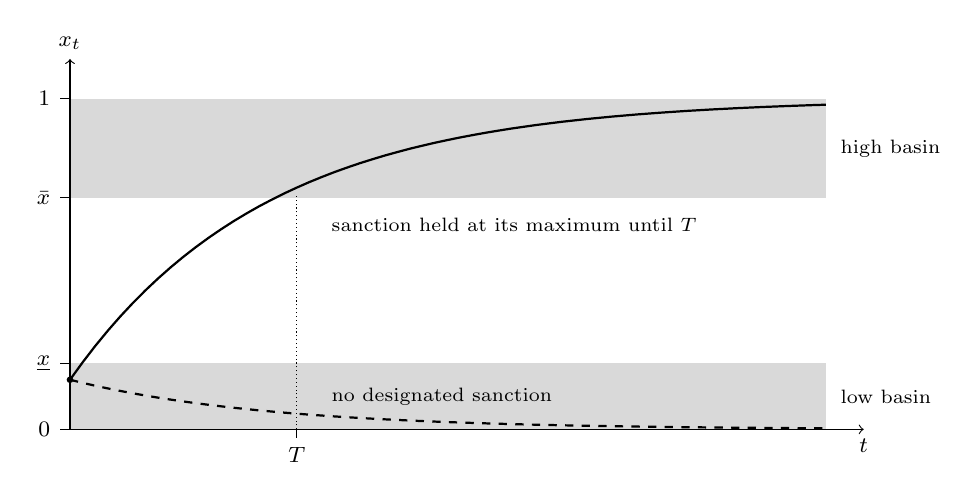
\begin{tikzpicture}[x=0.32cm,y=4.2cm,font=\footnotesize]
\fill[black!15] (0,0.7) rectangle (30,1);
\fill[black!15] (0,0) rectangle (30,0.2);
\draw[->] (0,0) -- (31.5,0) node[below] {$t$};
\draw[->] (0,0) -- (0,1.12) node[above] {$x_t$};
\foreach \y/\l in {0/0,0.2/\underline{x},0.7/\bar x,1/1} \draw (0,\y) -- (-0.4,\y) node[left] {$\l$};
\draw (9,0) -- (9,-0.025) node[below] {$T$};
\draw[densely dotted] (9,0) -- (9,0.71);
\draw[thick,domain=0:30,samples=61] plot (\x,{1-0.85*0.88^\x});
\draw[thick,dashed,domain=0:30,samples=61] plot (\x,{0.15*0.88^\x});
\fill (0,0.15) circle (1.2pt);
\node[anchor=west,font=\scriptsize] at (10,0.62) {sanction held at its maximum until $T$};
\node[anchor=west,font=\scriptsize] at (10,0.1) {no designated sanction};
\node[anchor=west,font=\scriptsize] at (30.2,0.85) {high basin};
\node[anchor=west,font=\scriptsize] at (30.2,0.1) {low basin};
\end{tikzpicture}
\caption{The path of the political state from the same start $x_0$ in the low basin
$[0,\underline x]$, under the partial-adjustment law. Dashed: without a designated
sanction the state stays in the low basin, where realized sanctions do not rise.
Solid: a sanction held at its maximum until date $T$ carries the state into the
high basin $[\bar x,1]$, after which equilibrium play keeps it there and the
sanction never falls (\Cref{prop:lock-in}).}
\label{fig:state-path}
\end{figure}

% @econ-contract paragraph
% id: DISC_BLUFFING
% role: Relate the designated sanction to bluffing under incomplete information (the author, 2026-10-17: "cite other paper's bluffing result ... they actually turn the bluffing to be true, and that caused the persist sanctions under this model"): a sanction imposed as a bluff, or to call one, and held long enough moves the state into the high basin, where continuing it is equilibrium play.
% depends_on: DISC_DESIGNATED_SANCTION
% handoff: Relief in practice.
% exact_ref: bib:Spaniel2015#pp=735-736,739
% source_role: bib:Spaniel2015#pp=735-736,739 => Under uncertainty about leader strength, weaker target leaders have incentives to bluff strength by continuing a crisis, and foreign powers sometimes call potential bluffs by implementing sanctions (read 2026-10-17 from the PDF); the bluffing result the paragraph builds on, not support for a result of this paper.
% exact_ref: bib:Brekhov2022#p=77
% source_role: bib:Brekhov2022#p=77 => Analyses targets' incentives to bluff under sanction (and reward) regimes in a repeated interaction with asymmetric information (read 2026-10-17 from the PDF); positioning only.
% exact_ref: tex-label:prop:lock-in
% support_status: VERIFIED
% status: PROPOSED
% @end-econ-contract
\central{Sanctions that begin as bluffs can become self-sustaining under equilibrium
play.} Under incomplete information, imposing sanctions can serve as a bluff or as a way
to call an opponent's bluff. In \citet[pp.~735--736]{Spaniel2015}, weaker target leaders
have ``incentives to bluff strength'' by continuing a crisis, and foreign powers respond
``by sometimes conceding and sometimes calling potential bluffs by implementing
sanctions''; \citet[p.~77]{Brekhov2022} analyzes target incentives to bluff under
sanctions. In those models, information revealed during the crisis determines subsequent
outcomes. Here, sanctions also shift the political state. A sanction imposed as a
bluff---or to call an opponent's bluff---and maintained for a sufficient duration acts as
a designated sanction in the sense defined above: it moves the state into the high basin,
where continued sanctioning is prescribed by equilibrium play. The bluff then becomes
self-fulfilling, and sanctions persist without any beliefs to revise.

\subsection{Real-world sanctions relief}
\label{sec:discussion:relief}
\label{sec:discussion:evidence}

% @econ-contract paragraph
% id: DISC_THREE_QUESTIONS
% role: Separate preference for relief, belief that it will be honoured, and its usability, and state the participation result (prop:relief-participation) at its scope, in words, as the model's answer to the first question.
% depends_on: DISC_BLUFFING
% handoff: Credibility of relief.
% merged_from: DISC_PARTICIPATION
% exact_ref: tex-label:prop:relief-participation
% support_status: NOT_APPLICABLE
% status: PROPOSED
% @end-econ-contract
\central{A natural application of the model is to proposals for sanctions relief, which raise
three related but distinct questions; the model's incentive comparisons speak to the
first.}\footnote{The participation
result is proved in \Cref{app:proofs:branch} of the Online Appendix; the economy
at which a temporary suspension of sanctions benefits a non-compliant target is recorded in the
formal supplement.}
Would policymakers prefer the arrangement and expect it to be honored, and would nominal
relief restore the economic activity it is intended to enable? On the first question,
consider a temporary suspension of sanctions followed by any equilibrium where the target
maintains full non-compliance, such as the constructed equilibrium. Under the
entrenchment condition and a sender response at full non-compliance that does not
decrease with the state, the change in incumbent payoffs does not support any date-zero
side payment between governments that would make the shock mutually acceptable. That
neither incumbent gains from such a shock follows jointly from three conditions: the
sender's positive marginal return to sanctioning a non-compliant target, the property
that compliance does not increase the sender's payoff at zero sanctions, and the
entrenchment condition. For an economy failing the entrenchment condition, a temporary
suspension of sanctions benefits a target that still does not comply.

% @econ-contract paragraph
% id: DISC_CREDIBILITY
% role: Tie the credibility of relief to commitment technologies and to lock-in, with the relief credibility point.
% depends_on: DISC_THREE_QUESTIONS
% handoff: Rival accounts of non-relief.
% exact_ref: bib:Powell2012#scope=paper
% source_role: bib:Powell2012#scope=paper => Already-cited source that singles out a costlessly reversible concession as least credible; it does not model this paper's state channel.
% support_status: UNVERIFIED
% status: PROPOSED
% @end-econ-contract
\central{The second question---whether relief will be honored---depends on commitment
technologies.} Lock-in depends on the initial state, and within a high basin resumed
equilibrium play generates no endogenous exit under the set and level conditions of
\Cref{prop:lock-in}. Expiry dates, review clauses, and other commitment technologies
operate by altering the strategic environment. Relief poses the hardest test for such
mechanisms. Relief that is reversible at no direct cost is the type that
\citet[p.~627]{Powell2012} identifies as least credible. In recent bargaining models of
war, the reliability of an agreement remains a parameter \citep{Ruggiero2026}. A full
model of relief institutions would need to specify, as separate primitives, who can
commit, who holds veto power, how private actors respond, and how these choices alter the
continuation game.

% @econ-contract paragraph
% id: DISC_RIVAL_ACCOUNTS
% role: Place rival accounts of non-relief without dismissing them as non-optimising (repair C6).
% depends_on: DISC_CREDIBILITY
% handoff: What the case material supports.
% exact_ref: bib:HalcoussisKaempferLowenberg2021#scope=paper
% source_role: bib:HalcoussisKaempferLowenberg2021#scope=paper => Already-cited legislative-cost account of sanction persistence; cited as an alternative, not as support for this model.
% support_status: UNVERIFIED
% status: PROPOSED
% @end-econ-contract
\central{Commitment problems are one explanation for persistent non-relief among
several; the model isolates a distinct mechanism.} In this mechanism, continued sanctions
can be optimal because of the state that sanctions have built, provided that the sender
values that target-side state and the entrenchment condition holds. Sanctions can be
optimal even if they are re-optimized every period and a lower sanction level is
feasible. Legislative constraints \citep{HalcoussisKaempferLowenberg2021}, administrative
persistence, and reputational incentives offer alternative explanations. Political or
reputational costs can themselves be incorporated into an optimizing decision
framework.

% @econ-contract paragraph
% id: DISC_PREDICTIONS
% role: State the two observable responses the classification separates, as model implications, not validation.
% depends_on: DISC_RIVAL_ACCOUNTS
% handoff: The case material.
% exact_ref: tex-label:thm:four-cells
% support_status: VERIFIED
% status: PROPOSED
% @end-econ-contract
\central{Comparisons across constructed equilibria distinguish two observable responses
to a single sanctions regime: greater compliance and deeper entrenchment.}\footnote{The
model's predictions are collected in \Cref{app:moved-ah} of the Online Appendix,
and the case sources' discussion of evasion and enforcement in
\Cref{app:moved-ad}.} Greater
compliance arises when the target's forward-looking incentive is weak and a
forward-looking sender raises the cost of relief; deeper entrenchment arises when that
incentive is strong and a forward-looking sender raises the steady-state level.

% @econ-contract paragraph
% id: DISC_CASE_MATERIAL
% role: Use the already-cited case material as motivation for the mechanism, with the Sender's stake kept as a maintained restriction.
% depends_on: DISC_PREDICTIONS
% handoff: The relief cases.
% exact_ref: bib:HaggardNoland2017#scope=paper
% source_role: bib:HaggardNoland2017#scope=paper => Already-cited account of an authoritarian target passing sanction costs to citizens; motivates the mechanism, does not identify any parameter.
% exact_ref: bib:UNPanelDPRK2024#scope=paper
% source_role: bib:UNPanelDPRK2024#scope=paper => Already-cited report of tighter control under sanctions; motivation only.
% support_status: UNVERIFIED
% status: PROPOSED
% @end-econ-contract
\central{North Korea, a context in which this feedback mechanism may be salient, helps
motivate the analysis.} \citet{HaggardNoland2017} describe an authoritarian target able
to pass sanction costs onto its citizens and a leadership reluctant to weaken its control
over foreign economic activity; in the model's terms, these correspond to low sanction
pain and a high valuation of the state---the two sides of the entrenchment condition. A
United Nations Panel of Experts report documents tighter economic, social, and political
controls and more centralized economic management under sanctions
\citep{UNPanelDPRK2024}. These same sources document evasion, enforcement, and
coordination challenges, which can coexist with the political-state feedback
mechanism.

% @econ-contract paragraph
% id: DISC_CASE_RELIEF
% role: Use the Iranian and Russian relief material (note N134, promoted 2026-10-02) to separate acceptability, credibility and delivery of relief, as motivation only.
% depends_on: DISC_CASE_MATERIAL
% handoff: The limits of the equilibrium interpretation.
% exact_ref: tex-label:sec:discussion:relief
% exact_ref: bib:BajoghliNasrSalehiIsfahaniVaez2024#pp=115-116,121-123
% source_role: bib:BajoghliNasrSalehiIsfahaniVaez2024#pp=115-116,121-123 => The authors' account (read 2026-10-02) that the prospect of lifting brought Iran to the 2015 agreement while rollback was slow, could be blocked or reimposed through Congress, and was made immaterial by remaining financial sanctions; motivation for separating the three relief questions, not a test of the model.
% exact_ref: bib:SnegovayaFentonDolbaiaBergmann2025#pp=26,31-32
% source_role: bib:SnegovayaFentonDolbaiaBergmann2025#pp=26,31-32 => The report's description (read 2026-10-02) of Russian businesses that thrive under isolation and fear returning competition, against firms that would gain from partial relief, with its scenario assumptions; heterogeneous interests, projections rather than observed outcomes.
% support_status: UNVERIFIED
% status: PROPOSED
% @end-econ-contract
\central{Iran and Russia illustrate all three questions raised above.} According to
\citet[pp.~115--116]{BajoghliNasrSalehiIsfahaniVaez2024}, the prospect of earlier
sanctions being lifted---not the threat of additional sanctions---brought Iran to the 2015
agreement. Yet the rollback was gradual and required political support at multiple levels
of the United States government. Congress, which is often involved in delisting
decisions, could impose additional hurdles or reimpose the same sanctions under another
pretext, and sanctions remaining on Iran's financial and banking system made the lifting
of others immaterial (pp.~121--123). Accepting relief, expecting it to be honored, and
being able to benefit from it are therefore distinct margins. In Russia, businesses that
have thrived under reduced competition fear the return of Western competitors, while
import- and export-dependent firms could gain from partial sanctions relief
\citep[pp.~31--32]{SnegovayaFentonDolbaiaBergmann2025}. The report's scenarios are
projections from 2025 (p.~26). This heterogeneity is what the political state variable
summarizes.

\subsection{Scope and limitations}
\label{sec:discussion:scope}

% @econ-contract paragraph
% id: DISC_SCOPE
% role: State the mechanism the model isolates and the object of its theorems for a specified instrument and compliance demand; effectiveness judged against a sender's objectives; how the class specializes to other coercive systems.
% depends_on: DISC_CASE_RELIEF
% handoff: The equilibrium concept and the results that reach beyond the constructed equilibria (repair C2).
% exact_ref: bib:GAO2025RussiaSanctions#pp=14
% source_role: bib:GAO2025RussiaSanctions#pp=14 => The report's three categories of objectives (read 2026-10-02); names the objectives against which effectiveness is judged, supports no model result.
% support_status: NOT_APPLICABLE
% status: PROPOSED
% @end-econ-contract
\central{We have deliberately isolated one public-choice mechanism behind persistent sanctions:
sanctions strengthen the target-side constituency that supports their continuation, and
both governments value that constituency.} Within the class, compliance affects the
sender by reducing its incentive to sanction. Given a coercive instrument and a
compliance demand, the theorems characterize how equilibrium play evolves from the
political state that sanctions---once imposed---have altered. Effectiveness, by contrast,
is measured against a sender's objectives, which the U.S. Government Accountability
Office identifies for U.S. measures on Russia as economic pressure, inhibition of the war
effort, and accountability \citep[p.~14]{GAO2025RussiaSanctions}. The mathematical
structure of the class can be adapted to other coercive systems. Doing so requires
mapping their actions, constituency effects, and payoff signs into the class structure,
including analogues of each government's stake in the state and of the entrenchment
condition.

% @econ-contract paragraph
% id: MODEL_EQUILIBRIUM_SCOPE
% role: How existence is obtained (by construction on invariant sets of value functions), and the concept against strong stationary Stackelberg and history-dependent equilibria (moved from Section 2.4, 2026-10-16, structure plan S4).
% depends_on: DISC_SCOPE
% handoff: The objects solved jointly and the results beyond the constructed equilibria.
% exact_ref: tex-label:thm:existence
% exact_ref: bib:HeLiuChen2025#scope=paper
% source_role: bib:HeLiuChen2025#scope=paper => Already-cited dynamic feedback Stackelberg existence and computation antecedent (restored 2026-10-02 after the rebuild dropped it); positions the joint-iteration existence route, does not prove it.
% exact_ref: bib:LiSojoudiTomlinFridovichKeil2024#scope=paper
% source_role: bib:LiSojoudiTomlinFridovichKeil2024#scope=paper => Already-cited feedback Stackelberg computation antecedent (restored 2026-10-02 after the rebuild dropped it); positioning only.
% exact_ref: tex-label:prop:history-deviations
% support_status: VERIFIED
% status: PROPOSED
% @end-econ-contract
\central{Existence is established by construction, and each construction pins down its
equilibrium only within the sets of value functions it employs.} Where the results
construct a value function, it is the unique fixed point of its Bellman operator defined
over an explicitly stated \emph{invariant set of value functions}: a closed set with
stated bounds on the level and slope of each member (and on
curvature for the sender), which the operator maps into itself. \Cref{sec:results} constructs
equilibria over the full class of economies. A general existence argument---based on
joint contraction of both Bellman equations when the coupling between them is
sufficiently weak---follows in the spirit of \citet{StokeyLucas1989} and of broader
research on the existence and computation of dynamic feedback Stackelberg equilibria
\citep{HeLiuChen2025,LiSojoudiTomlinFridovichKeil2024}.

\central{Two comparisons delineate the scope of the equilibrium concept: with the
stationary strong Stackelberg equilibrium, and with history-dependent strategies.}
First, target optimality in $\mathcal E$ is pointwise: at each state, the target
maximizes the right-hand side of \eqref{eq:T-bellman}, taking continuation values as
given. In a stationary strong Stackelberg equilibrium, by contrast, the leader selects an
entire policy function and anticipates that the follower re-optimizes after every policy
deviation; the two concepts need not coincide \citep{Bucarey2023,KudoAkimoto2026}. The
equilibrium concept is time-consistent because both governments re-optimize at every
state. Second, against any equilibrium in $\mathcal E$, no pure strategy conditioned on
the entire history outperforms the equilibrium's own play, from any initial state
and---for the sender---after any observed compliance level on or off the equilibrium
path.

% @econ-contract paragraph
% id: DISC_EQUILIBRIUM_LIMITS
% role: State the equilibrium notion, the objects it solves jointly, and the two results that reach beyond the constructed equilibria (repair C2).
% depends_on: MODEL_EQUILIBRIUM_SCOPE
% handoff: Levels of generality.
% merged_from: DISC_ENDOGENOUS
% exact_ref: tex-label:prop:security
% note: 2026-10-16 (structure plan S4): the Markov sentence is in Section 2.4 and the minmax and uniqueness results in Section 3.4; this paragraph points there.
% support_status: VERIFIED
% status: PROPOSED
% @end-econ-contract
\central{Within each equilibrium, the target's compliance rule, the sender's sanction
rule, both value functions, both feedback policies, and the political-state trajectory
are solved jointly.} In the interest-group polity, the pressure levels of competing
groups also constitute a Nash equilibrium of the political contest. Two results extend
beyond the constructed equilibria under the strong entrenchment condition: the target's
minmax payoff bound and the uniqueness of full non-compliance among non-decreasing
sanction rules (\Cref{sec:results:security}).

% @econ-contract paragraph
% id: DISC_GENERALITY_LEVELS
% role: Separate results about every equilibrium satisfying stated conditions, results derived from primitives on the class, and results established at example economies, citing main-text results only.
% depends_on: DISC_EQUILIBRIUM_LIMITS
% handoff: Open extensions.
% exact_ref: tex-label:prop:certified-equilibria
% support_status: VERIFIED
% status: PROPOSED
% @end-econ-contract
\central{The results operate at three levels of generality.} First, some apply to every
equilibrium satisfying stated conditions: lock-in (\Cref{prop:lock-in}) applies to every
equilibrium meeting its basin conditions and, for entry, its transition conditions; the
fixed-target-policy comparison (\Cref{thm:dominance}) applies to every non-decreasing
sender value at every state, and thus to every equilibrium containing one; the premium bound
of \Cref{sec:results:wedge} applies to every equilibrium with a non-increasing target
policy, for economies in the class with an upper bound on the substitution rate at which
larger concessions are never worth more to the sender at zero sanctions; and the minmax
bound applies to every equilibrium in $\mathcal E$. Second, the myopic-benchmark
comparison (\Cref{thm:regime-separation}), the four-case characterization
(\Cref{thm:four-cells}), and the threshold result (\Cref{prop:collapse-threshold}) derive
equilibrium properties and dynamics from inequalities across primitives over the class, and
greater target patience preserves the full-non-compliance equilibrium that exists at a
lower discount factor (\Cref{prop:patience-existence}). The welfare results of
\Cref{sec:welfare} hold across the class, as do the rescaling property and the planner
optimality condition for any representation and any bounded welfare flow. Third, some
results are established via example economies, which demonstrate that hypotheses can be
satisfied or bounds attained: the welfare loss in one interest-group polity
(\Cref{sec:welfare:efficiency}), the attainment of the premium bound
(\Cref{sec:results:wedge}), and economies satisfying the lock-in conditions
(\Cref{app:persistence:reading} of the Online Appendix).

% @econ-contract paragraph
% id: DISC_OPEN
% role: Name the extensions and the measurement requirements for empirical work.
% depends_on: DISC_GENERALITY_LEVELS
% handoff: The conclusion.
% exact_ref: bib:AttiaGrauvogel2023#scope=paper
% source_role: bib:AttiaGrauvogel2023#scope=paper => Already-cited exploratory association between institutional clauses and termination; not a causal estimate and not support for a model result.
% support_status: UNVERIFIED
% status: PROPOSED
% @end-econ-contract
\central{Two broad kinds of extensions build on these results: empirical measurement of
the political state and its associated payoff terms, and richer theoretical models of
the state and of relief institutions.} Disciplining estimates of the political-state
transition and the payoff terms governing basin entry would require empirical measures
that separate the political state from aggregate income, and distinguish within-target
adjustment from selection across surviving episodes. Theoretical extensions could
incorporate multidimensional political states, stochastic shock duration,
forward-looking investment by groups in their own future power
\citep{AcemogluRobinson2008}, or explicit relief and commitment technologies. The last of
these could alter entry into or create exit from the high basin, and
\citet{AttiaGrauvogel2023} document exploratory empirical associations between such
provisions and sanction termination. A fully optimal relief policy would require explicit
institutional instruments and commitment constraints. A symmetric framework in which both
governments directly move the state---of the kind \citet{Powell2013} calls for---would
embed compliance directly into the transition law and require rederiving the argument
that compliance reduces the sender's incentive to sanction.

% @econ-contract include
% id: INCLUDE_CONCLUSION
% file: main_sections/06_conclusion.tex
% section_contract: CONCLUSION_ANSWER
% role: Answer the question at its proved scope and state its limits.
% question_answered: What was established, and where does it stop?
% required_inputs: All result sections.
% output_handoff: None.
% claim_ceiling: The master plan's ceiling; no policy prescription.
% status: HUMAN_CONFIRMED
% @end-econ-contract
% @econ-contract section
% id: CONCLUSION_ANSWER
% role: Answer the question at its proved scope: the mechanism and answer first; who decides accommodation, who decides intensity; what the reach results add; the persistence and welfare limits.
% question_answered: What did the paper establish, and where does it stop?
% required_inputs: RESULTS_HORIZONS, WELFARE_BOUNDARY, DISCUSSION_INTERPRETATION.
% output_handoff: None.
% claim_ceiling: The master plan's ceiling; no policy prescription.
% exclusions: A theorem list; new claims.
% exact_ref: tex-label:sec:conclusion
% support_status: VERIFIED
% status: HUMAN_CONFIRMED
% human_confirmed_at: 2026-10-01
% decision_ref: suggestions/2026-10-01-manuscript-rebuild/01_STRUCTURE_PROPOSAL.md#author-decisions-recorded
% confirmation_scope: Section role and claim ceiling.
% reopen_if: A principal result or the claim ceiling changes.
% amended_at: 2026-10-12 (opens on the dual-basin illustration and states its limits; decision_ref: suggestions/2026-10-10-jet-submission/DECISIONS.md#framing-2026-10-12); 2026-10-13 (argument plan: mechanism and answer first, then the dual-basin illustration with its limits, the reach results, welfare and lock-in, and a closing 'so what / now what' paragraph; decision_ref: suggestions/2026-10-10-jet-submission/exposition-2026-10-13/ARGUMENT_PLAN.md); 2026-10-15 (the dual-basin illustration dropped from the main text for now, on the author's word); 2026-10-19 (coauthor wording review: wording of the coauthor's line-by-line revision applied where not wrong; sender/target in lower case; non-compliance for defiance; decision_ref: suggestions/2026-10-10-jet-submission/DECISIONS.md#coauthor-wording-review-2026-10-19); 2026-10-20 (humanizer pass: dashes replaced by commas, parentheses or colons; plain wording; meaning unchanged; decision_ref: suggestions/2026-10-10-jet-submission/DECISIONS.md#humanizer-pass-2026-10-20)
% @end-econ-contract
\section{Conclusion}
\label{sec:conclusion}

% @econ-contract paragraph
% id: CONCLUSION_ROLES
% role: Open with the mechanism and the answer on the class (the myopic benchmark ends sanctions, forward-looking governments sustain them; the Target's patience decides relief against defiance), then the Sender's role and the same-policy comparison with its hypothesis (repair C4). Moved first (argument plan, 2026-10-13); reordered on the layout decisions of 2026-10-16.
% depends_on: CONCLUSION_ANSWER
% handoff: The reach results.
% exact_ref: tex-label:prop:myopic-benchmark
% exact_ref: tex-label:thm:regime-separation
% exact_ref: tex-label:thm:four-cells
% exact_ref: tex-label:thm:dominance
% support_status: VERIFIED
% status: PROPOSED
% @end-econ-contract
\central{Economic sanctions can persist because they strengthen the domestic political
interests that support their continuation.} Without foresight they unravel: in the
myopic benchmark, the target accommodates and the political state erodes over time. In
the equilibria constructed over the class of economies, when both governments value the
political state and are forward-looking, the target maintains non-compliance, sanctions
persist indefinitely, and the political state converges to a positive steady-state
level. The target's patience determines whether relief or non-compliance prevails;
whether the sender is forward-looking shapes the compliance threshold for relief or the
intensity of sanctions under non-compliance. These comparisons hold all non-discount
primitives fixed. For a fixed target policy, a non-decreasing sender continuation value
weakly increases the largest of the optimal sanctions relative to the myopic best response. Under
interiority, the constructed equilibria exhibit a strictly positive foresight premium
relative to the myopic best response, with a closed-form lower bound.

% @econ-contract paragraph
% id: CONCLUSION_REACH
% role: Summarize the reach results: patience, like the Target's other parameters, can change whether full defiance is an equilibrium; result names in place of condition lists (argument plan, 2026-10-13).
% depends_on: CONCLUSION_ROLES
% handoff: The welfare findings and lock-in.
% exact_ref: tex-label:prop:security
% exact_ref: tex-label:prop:collapse-threshold
% support_status: VERIFIED
% status: PROPOSED
% @end-econ-contract
\central{Beyond the constructed equilibria, patience, like all other target
parameters, shapes whether full non-compliance is supportable as an equilibrium.} When
the sender's response and the target's value under full non-compliance do not decrease
with the state, greater target patience preserves the full-non-compliance equilibrium.
Under the strong entrenchment condition, the target guarantees itself a minmax payoff
against every pure sanction strategy, bounding its payoff in every equilibrium from
below; and across the class, every equilibrium with a non-decreasing sanction rule
exhibits full non-compliance. In the special case of \Cref{prop:collapse-threshold}, a
full-non-compliance equilibrium exists if and only if the target's discount factor is at
least a threshold value.

% @econ-contract paragraph
% id: CONCLUSION_LIMITS
% role: State the welfare findings, then lock-in and persistence without hysteresis, naming prop:lock-in instead of listing its conditions (argument plan, 2026-10-13).
% depends_on: CONCLUSION_REACH
% handoff: So what and now what.
% exact_ref: tex-label:sec:welfare
% exact_ref: tex-label:prop:lock-in
% support_status: VERIFIED
% status: PROPOSED
% @end-econ-contract
\central{Persistent sanctions can be socially costly, and the game alone does not
determine their welfare ranking.} Across the class, two interest-group representations
of the same government payoffs rank the constructed equilibria in opposite orders, and
under compliance neutrality one makes persistent play socially optimal. For an example
economy with one explicit interest-group polity, equilibrium sanctions remain at their
maximum level and generate welfare losses.

The political state can also lock in sanctions. Where an equilibrium and a high-state
interval satisfy the conditions of \Cref{prop:lock-in}, a state entering the interval
remains there under equilibrium play and sanctions never decline. When full sanctions
raise every state below the basin, a sufficiently long temporary shock can produce a
durable outcome. Persistence can also arise without hysteresis. Where the explicit
Lipschitz constant derived for the constructed equilibrium's law of motion is strictly
below one, a temporary shock has no permanent asymptotic effect.

% @econ-contract paragraph
% id: CONCLUSION_SO_WHAT
% role: Say what the results mean (persistence need not reveal failed bargaining or misperception; with information complete, the levers act on the political state and the governments' incentives, not on beliefs) and what would discipline the channel (measurement, sec:discussion:scope), with no prescription; close on the paper's answer.
% depends_on: CONCLUSION_LIMITS
% handoff: None.
% origin: argument plan item 10 (2026-10-13); the closing sentence moved here from CONCLUSION_LIMITS.
% exact_ref: tex-label:sec:discussion:scope
% exact_ref: tex-label:sec:discussion:misperception
% support_status: VERIFIED
% status: PROPOSED
% @end-econ-contract
\central{Persistent sanctions therefore need not reflect failed bargaining or
misperception.} Within the model, they can be the optimal choice of governments that
value the political state that sanctions themselves have built. With complete
information, the levers that end sanctions operate through the political state and
government incentives, not through beliefs (\Cref{sec:discussion:misperception} of the
Online Appendix). Whether this channel operates in a given episode is an empirical
question: measurements that separate the political state from aggregate income would
discipline estimates of its transition and of the payoff terms governing basin entry
(\Cref{sec:discussion:scope}). \central{Optimizing governments can thus perpetuate and
lock in sanctions through the political state that sanctions generate; patience and
other economic features determine whether this occurs.}

% @econ-contract include
% id: INCLUDE_DECLARATIONS
% file: main_sections/07_declarations.tex
% section_contract: DECLARATIONS_STATEMENTS
% role: Carry the required author declarations.
% question_answered: Competing interests, funding, contributions, AI use, data availability.
% required_inputs: Author records.
% output_handoff: None.
% claim_ceiling: Declarations only; no scientific claim.
% status: HUMAN_CONFIRMED
% @end-econ-contract
% @econ-contract section
% id: DECLARATIONS_STATEMENTS
% role: Carry the required author declarations.
% question_answered: Competing interests, funding, contributions, AI use, data availability.
% required_inputs: Author records.
% output_handoff: None.
% claim_ceiling: Declarations only; no scientific claim.
% exclusions: Any scientific claim.
% support_status: NOT_APPLICABLE
% status: HUMAN_CONFIRMED
% human_confirmed_at: 2026-10-01
% decision_ref: suggestions/2026-10-01-manuscript-rebuild/01_STRUCTURE_PROPOSAL.md#author-decisions-recorded
% confirmation_scope: Section role only; the declarations' content is the author's.
% reopen_if: Journal requirements or the author's declarations change.
% amended_at: 2026-10-19 (data availability names the release v1.30-submission; decision_ref: suggestions/2026-10-10-jet-submission/DECISIONS.md#submission-release-2026-10-19); 2026-10-20 (the repository link; decision_ref: suggestions/2026-10-10-jet-submission/DECISIONS.md#repository-link-and-acemoglu-notes-2026-10-20); 2026-10-20 (the release is public at the new repository; decision_ref: suggestions/2026-10-10-jet-submission/DECISIONS.md#public-repository-2026-10-20); 2026-10-21 (Elsevier layout: the generative-AI statement is its own section, titled as the Guide requires, last before the references, wording otherwise unchanged; funding in the Guide's sentence; data availability without the internal script name, citing the release; decision_ref: suggestions/2026-10-10-jet-submission/DECISIONS.md#jet-submission-package-2026-10-21)
% @end-econ-contract
\section*{Declarations}

% Coauthors' confirmation of no competing interests: received (the author, 2026-10-21).
\paragraph{Declaration of competing interest.} The authors declare no
competing financial interests or personal relationships that could have
influenced the work reported in this paper.

\paragraph{Funding.} This research did not receive any specific grant from funding
agencies in the public, commercial, or not-for-profit sectors.

\paragraph{CRediT author statement.} Xiaofeng Gong:
Conceptualization, Formal analysis, Methodology, Software, Validation,
Visualization, Writing -- original draft, and Writing -- review and
editing. Yuechuan Zhao: Conceptualization, and Writing -- review and
editing. Chunping Zhong: Conceptualization, and Writing -- review and
editing.

\paragraph{Data availability.} No empirical data were used. The Lean~4 formalization
that machine-checks the core results of this paper, as mapped in the formal supplement, is
public as the release \texttt{v1.30-submission} at
\url{https://github.com/qidaolake/political-entrenchment-sanctions-lean}
\citep{GongLean2026}, with the manuscript, the Online Appendix and the formal supplement
attached to it. Its source archive accompanies this submission as supplementary material.
A deposit with a DOI will accompany publication.

\paragraph{Formalization methods.} The Lean~4 development was written with
assistant-generated suggestions for proof steps and lemma search. The
selection of the statements to formalize, the economic interpretation of
every formal statement, and the correspondence map between the manuscript
and the declarations were made and reviewed by the authors, and the Lean~4
kernel independently checks every proof term in the archived release. A
kernel check certifies a formal statement; it does not certify that an
informal economic sentence translates that statement faithfully, which is
why the correspondence is recorded as a separately reviewed map in the
formal supplement.


% ---------------------------------------------------------------------
% COMBINED mode only: inline the appendix so that a single PDF carries
% both the manuscript and the appendix under one bibliography.
% ---------------------------------------------------------------------


\ifdefined\COMBINEDAPPENDIX
% @econ-contract include
% id: INCLUDE_APPENDIX_BODY
% file: sanctions_appendix_body.tex
% section_contract: APPENDIX_INDEX
% role: Inline the appendix in the combined build only; the split build cross-references the standalone appendix.
% question_answered: Where are the exact statements, proofs, constructed economies and the formalization map?
% required_inputs: All main sections.
% output_handoff: None.
% claim_ceiling: Exact statements and proofs of the results the main text states; no further claim.
% status: HUMAN_CONFIRMED
% @end-econ-contract
  % @econ-contract section
% id: APPENDIX_INDEX
% role: Order the appendix in three parts: general results for abstract payoffs and transitions in the class (conditions and component statements, proofs, persistence and lock-in, existence, discharge routes, supporting results, further statements); examples (parametric families and the roster, numerical economies, closed-form constants, the interest-group example); the literature (the author's decision, 2026-10-20); within each part, what the main text needs comes before derivative and supplementary material (2026-10-20).
% question_answered: Where is each exact statement and proof?
% required_inputs: The main sections.
% output_handoff: None.
% claim_ceiling: Exact statements and proofs of results the main text states; machine-checked statements as recorded in the formalization map.
% exclusions: New claims not stated or summarised in the main text.
% exact_ref: file:appendix_sections/07_formalization_map.tex#label=app:formalization
% source_role: file:appendix_sections/07_formalization_map.tex#label=app:formalization => The formal supplement's formalization map, which records the Lean declaration behind each statement; it establishes formal derivation, not economic correspondence.
% support_status: VERIFIED
% status: HUMAN_CONFIRMED
% human_confirmed_at: 2026-10-01
% decision_ref: suggestions/2026-10-01-manuscript-rebuild/01_STRUCTURE_PROPOSAL.md#author-decisions-recorded
% confirmation_scope: Appendix role and the D1 moves.
% amended_at: 2026-10-20 (three parts, general results and examples separated, on the author's "see whether we can have a generalized form abstract functional form appendix versus a numerical example appendix please, make it more organized"; decision_ref: suggestions/2026-10-10-jet-submission/DECISIONS.md#appendix-in-three-parts-and-the-one-sided-cases-paragraph-2026-10-20); 2026-10-20 (within each part, what the main text needs before derivative material; decision_ref: suggestions/2026-10-10-jet-submission/DECISIONS.md#appendix-needed-versus-derivative-2026-10-20); 2026-10-20 (proof maps open Part I; decision_ref: suggestions/2026-10-10-jet-submission/DECISIONS.md#proof-maps-and-reading-the-lean-statements-2026-10-20)
% reopen_if: A section moves between the main text and the appendix.
% @end-econ-contract
% =====================================================================
%  SHARED APPENDIX INDEX  --  sanctions_appendix_body.tex
%
%  This file is NOT a document.  It is \input by BOTH:
%     sanctions_jet_appendix.tex   -> standalone appendix PDF
%     sanctions_jet_draft.tex      -> only in COMBINED mode
%  so the two builds cannot diverge.  It begins at \appendix, inputs the
%  ordered files under appendix_sections/, and ends before the bibliography,
%  which each root supplies for itself.
% =====================================================================

\appendix

% Everything below is an appendix, so cleveref must call it one.  Without
% these two lines \Cref{app:closedforms} typesets as "Section C" -- which,
% now that the appendix is a separate document, names a section the
% manuscript does not contain.  (The \crefnames are in sanctions_preamble.tex.)
\crefalias{section}{appendix}
\crefalias{subsection}{subappendix}
\crefalias{subsubsection}{subappendix}

% Ordered appendix-section index; section bodies live in appendix_sections/.
\input{appendix_sections/00_notation}

% A group heading inside a part: what the main text needs, then derivative material.
\providecommand{\appendixgroup}[1]{\par\bigskip\noindent{\large\bfseries #1}\par\nopagebreak\medskip}

% Part I: results that hold for abstract payoffs and transitions in the class.
\part{General results: abstract payoffs and transitions}
\appendixgroup{What the main text needs: the conditions, the construction and the proofs}
\input{appendix_sections/15_proof_maps}
\input{appendix_sections/11_moved_statements_2026_10_13}
\input{appendix_sections/01_headline_proofs}
\input{appendix_sections/09_persistence_and_imposed_episodes}
\input{appendix_sections/13_decomposition_and_path}
\appendixgroup{Derivative and supplementary results}
\input{appendix_sections/06_existence_and_long_run_law}
\input{appendix_sections/02_assumption_discharge_routes}
\input{appendix_sections/07_supporting_results}
\input{appendix_sections/08_moved_statements}

% Part II: parametric families and numerical economies.
\part{Examples: parametric families and numerical economies}
\appendixgroup{The examples the main text uses}
\input{appendix_sections/04_witness_parameter_vectors}
\input{appendix_sections/12_numerical_examples}
\input{appendix_sections/05_microfounded_four_group_witness}
\appendixgroup{Further examples and constants}
\input{appendix_sections/14_further_examples}
\input{appendix_sections/03_closed_form_constants}

% Part III: the literature.
\part{Literature}
\input{appendix_sections/10_related_literature}

\fi

\bibliographystyle{econ-aea}
\bibliography{annote}

\end{document}
"
%
%  New paper material does NOT get written here first.  It lands in an
%  appropriate file under note_sections/ and is promoted only on the author's decision
%  (project rule: CLAUDE.md Rule 21).
% =====================================================================

% =====================================================================
%  SHARED PREAMBLE  --  sanctions_preamble.tex
%
%  Included by all four root documents:
%     sanctions_jet_draft.tex      (the submission manuscript)
%     sanctions_jet_appendix.tex   (the appendix reference document)
%     sanctions_jet_notes.tex      (the staging / other-information document)
%     sanctions_formal_supplement.tex (the online formal-verification supplement)
%
%  This file is NOT a document.  It carries only packages, theorem
%  environments, and macros, so the four roots cannot drift apart in
%  notation.  Anything document-specific (title, numbering scheme,
%  \externaldocument wiring) belongs in the root that needs it.
% =====================================================================

% ---------- Packages ----------
\usepackage[margin=1in]{geometry}
\usepackage{amsmath,amssymb,amsthm,mathtools}
\usepackage{enumitem}
% xr-hyper resolves \ref/\Cref/\eqref/\cite targets that live in a sibling
% document (main <-> appendix <-> notes).  It MUST be loaded before hyperref.
\usepackage{xr-hyper}
\usepackage[hidelinks]{hyperref}
\usepackage[nameinlink,capitalize]{cleveref}
\usepackage{aliascnt}
% thmtools removed 2026-08-07.  It was loaded but never used --- no
% \declaretheorem, no \listoftheorems, nothing but the \usepackage line ---
% and its current release (v0.76, 2023-05-04) patches \newtheorem in a way
% that breaks a shared-counter declaration such as
% \newtheorem{lemma}[theorem]{Lemma} under the 2026-06-01 LaTeX kernel
% ("Command \c@lemma already defined").  No newer thmtools is available.
% The theorem block below uses only amsthm, which handles it correctly.
\usepackage{booktabs}
\usepackage{array}
\usepackage{longtable}
\usepackage[expansion=false]{microtype}
\usepackage{graphicx}
\usepackage{caption}
\usepackage{natbib}
\usepackage{xurl}
\urlstyle{tt}
\usepackage{tikz}
\usetikzlibrary{arrows.meta,positioning,fit,backgrounds,calc,shapes.geometric}
\usepackage{pdflscape}

% ---------- Theorem Environments ----------
% Lemmas, propositions, corollaries, definitions and remarks share the theorem counter through
% alias counters (2026-10-11), so that cleveref names each by its own type: with a plain shared
% counter every \Cref of a proposition printed "Theorem". Their numbers expand to \thetheorem at
% print time, so the appendix's \numberwithin{theorem}{section} numbers them A.1, A.2, ... as before.
\theoremstyle{plain}
\newtheorem{theorem}{Theorem}
\newaliascnt{lemma}{theorem}
\newtheorem{lemma}[lemma]{Lemma}
\renewcommand{\thelemma}{\thetheorem}\renewcommand{\theHlemma}{\theHtheorem}
\crefname{lemma}{Lemma}{Lemmas}\Crefname{lemma}{Lemma}{Lemmas}
\newaliascnt{proposition}{theorem}
\newtheorem{proposition}[proposition]{Proposition}
\renewcommand{\theproposition}{\thetheorem}\renewcommand{\theHproposition}{\theHtheorem}
\crefname{proposition}{Proposition}{Propositions}\Crefname{proposition}{Proposition}{Propositions}
\newaliascnt{corollary}{theorem}
\newtheorem{corollary}[corollary]{Corollary}
\renewcommand{\thecorollary}{\thetheorem}\renewcommand{\theHcorollary}{\theHtheorem}
\crefname{corollary}{Corollary}{Corollaries}\Crefname{corollary}{Corollary}{Corollaries}

% Appendix sections must be cited as "Appendix C", never "Section C".
% This mattered little while the paper was one document; once the appendix
% is its own artefact, "Section C" points at a section the manuscript does
% not have.  The \crefalias that activates these lives immediately after
% \appendix in the shared sanctions_appendix_body.tex index, so it applies in BOTH the
% standalone appendix build and the COMBINED build.
\crefname{appendix}{Appendix}{Appendices}
\Crefname{appendix}{Appendix}{Appendices}
\crefname{subappendix}{Appendix}{Appendices}
\Crefname{subappendix}{Appendix}{Appendices}

\theoremstyle{definition}
\newtheorem{assumption}{Assumption}
\newaliascnt{definition}{theorem}
\newtheorem{definition}[definition]{Definition}
\renewcommand{\thedefinition}{\thetheorem}\renewcommand{\theHdefinition}{\theHtheorem}
\crefname{definition}{Definition}{Definitions}\Crefname{definition}{Definition}{Definitions}
\crefname{assumption}{Assumption}{Assumptions}
\Crefname{assumption}{Assumption}{Assumptions}

\theoremstyle{remark}
\newaliascnt{remark}{theorem}
\newtheorem{remark}[remark]{Remark}
\renewcommand{\theremark}{\thetheorem}\renewcommand{\theHremark}{\theHtheorem}
\crefname{remark}{Remark}{Remarks}\Crefname{remark}{Remark}{Remarks}

% ---------- Commands ----------
% Central sentence of a paragraph (2026-10-11): each paragraph's central sentence is wrapped in
% \central{...}. It prints as ordinary text; sanctions_jet_review.tex defines \centralmarks before
% loading the draft, which colours every central sentence for review.
\ifdefined\centralmarks
  \newcommand{\central}[1]{\textcolor{blue!55!black}{#1}}
\else
  \newcommand{\central}[1]{#1}
\fi
\newcommand{\R}{\mathbb{R}}
% Indicator. Was \mathbbm{1} from the bbm package; bbm lives in
% texlive-fonts-extra, which the CI TeX subset does not install, and the
% macro is used nowhere in the three documents. \mathbf carries the same
% glyph role with no extra package. Restore bbm here if the
% blackboard-bold indicator is ever wanted.
\newcommand{\1}{\mathbf{1}}
\newcommand{\Us}{U_S}
\newcommand{\Ut}{U_T}
\newcommand{\Vs}{V_S}
\newcommand{\Vt}{V_T}
\newcommand{\basin}{\mathcal{B}}
\newcommand{\sigDyn}{\sigma^{\mathrm{dyn}}}
\newcommand{\sigDynTop}{\sigma^{\mathrm{dyn}}}
\newcommand{\alphaM}{\alpha^{\mathrm{M}}}
\newcommand{\sigM}{\sigma^{\mathrm{M}}}
\newcommand{\F}{F}
\newcommand{\JSgroup}{\mathsf{J}_S}
\newcommand{\KSgroup}{\mathsf{K}_S}
\newcommand{\JTgroup}{\mathsf{J}_T}
\newcommand{\KTgroup}{\mathsf{K}_T}


% Resolve \Cref{app:...} etc. against the standalone appendix document.
% In COMBINED mode the appendix labels are defined locally, so importing
% them again would collide -- hence the guard.
\ifdefined\COMBINEDAPPENDIX\else
  \externaldocument[][nocite]{sanctions_jet_appendix}
\fi
\externaldocument[][nocite]{sanctions_formal_supplement}

\title{Political Entrenchment and the Persistence of Economic Sanctions}
% Corresponding author. Add ORCID iD before submission
% (Elsevier Editorial Manager requires both for the corresponding author).
\author{Xiaofeng Gong\thanks{Corresponding author. Department of
Economics, University of Connecticut, 365 Fairfield Way, Unit 1063,
Storrs, CT 06269-1063, USA. Email:
\texttt{xiaofeng.gong@uconn.edu}. Telephone: +1 857-384-2289.}
\and Yuechuan Zhao\thanks{National Academy of Economic Strategy, Chinese Academy of
Social Sciences, Beijing, China. Email: \texttt{zhaoyuechuan@ucass.edu.cn}.}
\and Chunping Zhong\thanks{National Academy of Economic Strategy, Chinese Academy of
Social Sciences, Beijing, China. Email: \texttt{cpzenith@163.com}.}}
\date{October 2026}

% @econ-contract master
% id: PAPER_MASTER_PLAN
% central_question: When sanctions move a political state that both governments value, can forward-looking incentives make sanctions persist where myopic ones would end them, and what does each government's foresight contribute?
% provisional_answer: At common non-discount primitives on the stated class, the myopic benchmark ends sanctions through relief while forward-looking governments sustain them under defiance with a positive long-run state; the Target's horizon decides accommodation against defiance and the Sender's horizon decides the compliance that relief buys or the sanction sustained under defiance; the defiance channel extends beyond the displayed profiles at stated quantifiers, and government incentives do not identify the social ranking.
% claim_ceiling: The myopic benchmark and the constructed forward-looking equilibrium, and the four cases in the discussion; existence inheritance under monotonicity hypotheses; a value bound in every top-selector equilibrium; uniqueness only in the nondecreasing-rule class; exactness only on the tight collapse class; welfare non-identification on the class by two representations, a sufficient condition for planner-optimal zero sanctions, and one representation under which full-defiance play is planner-optimal; no global uniqueness, complete classification, empirical or policy claim.
% principal_result_chain: Equilibrium environment and the myopic benchmark; the forward-looking equilibrium against it, with the Target's part and the Sender's wedge and same-policy dominance; lock-in; scope of the defiance channel (patience, security value, identification, certificates, exact collapse); welfare boundary; persistence is not hysteresis.
% reader_order: Abstract; Introduction (with literature); Model; Equilibrium and comparative statics; Welfare; Discussion; Conclusion; Appendix.
% build_order: Appendix intake; Model; Equilibrium and comparative statics; Welfare; Discussion; Introduction; Abstract; Conclusion.
% source_layout: SECTION_OWNED
% canonical_entrypoint: sanctions_jet_draft.tex
% status: HUMAN_CONFIRMED
% human_confirmed_at: 2026-10-01
% decision_ref: suggestions/2026-10-01-manuscript-rebuild/01_STRUCTURE_PROPOSAL.md#author-decisions-recorded
% confirmation_scope: Question, answer, claim ceiling, result chain, section order (D1), main-text propositions (D2, D5), headline pinning (D4).
% reopen_if: The question, the claim ceiling, the order of the principal moves, or the section layout changes.
% @end-econ-contract

\begin{document}

\maketitle

% @econ-contract paragraph
% id: ABSTRACT_SUMMARY
% role: State the model and its mechanism in the manner of Acemoglu and coauthors (N185), then the claims at their proved scope (the roles of the two governments' patience in the constructed equilibria, lock-in, welfare beyond the example economy, the Lean check), with no manuscript notation.
% amended_at: 2026-10-11 (fewer claims, lock-in added; the author: "cut down the number of the things on the abstract"); 2026-10-13 (argument plan: the problem first, "we show", "in one equilibrium", "beyond the example economy"; same claims); 2026-10-19 (coauthor wording review: wording of the coauthor's line-by-line revision applied where not wrong; sender/target in lower case; non-compliance for defiance; decision_ref: suggestions/2026-10-10-jet-submission/DECISIONS.md#coauthor-wording-review-2026-10-19); 2026-10-20 (N185 promoted: "We develop a dynamic model", the environment in plain sentences, the claims and their scope words unchanged, the Lean 4 sentence kept on the author's "maybe still add the usage of lean 4"; decision_ref: suggestions/2026-10-10-jet-submission/DECISIONS.md#acemoglu-comparison-and-model-exposition-2026-10-20)
% depends_on: PAPER_MASTER_PLAN
% handoff: The introduction.
% exact_ref: tex-label:sec:results
% support_status: VERIFIED
% status: PROPOSED
% @end-econ-contract
\begin{abstract}
\central{We develop a dynamic model in which economic sanctions shift the balance of
political power within the target country.} Each period the target chooses how far
to comply and the sender responds with sanctions. Sanctions raise political
entrenchment, the de facto power of target-side constituencies aligned with continued
confrontation, and both governments value this state. For a general class of economies, the
model provides conditions under which myopia makes sanctions unravel: the target
adjusts compliance just enough to induce sanction removal. When both governments are
forward-looking, the target maintains non-compliance and sanctions persist
indefinitely, even under complete information. The target's patience determines
whether relief or non-compliance prevails, while a forward-looking sender raises the
steady-state level of political entrenchment. Under stated conditions, a sufficiently
long temporary sanction shock locks in persistent sanctions. The game alone does not
pin down a welfare ranking. The core results are formally verified via machine-checked
proofs in Lean~4.
\end{abstract}

\medskip
\noindent\textbf{Keywords:} economic sanctions; persistence and
hysteresis; dynamic political economy; feedback Stackelberg equilibrium;
political entrenchment; path dependence.

\smallskip
\noindent\textbf{JEL classification:} C73; D72; F51; C61; D74.

% Elsevier Highlights are submitted separately and are intentionally
% omitted from the manuscript PDF.

% Section files follow the thin-root layout used by the reference project.
% @econ-contract include
% id: INCLUDE_INTRO
% file: main_sections/01_introduction.tex
% section_contract: INTRO_FRAME
% role: Pose the question and the experiment, state the three contributions at proved strength, and place them in the literature.
% question_answered: What question, how, and with what claim ceiling?
% required_inputs: All result sections (written last).
% output_handoff: Question, answer, ceiling and roadmap.
% claim_ceiling: The master plan's ceiling.
% status: HUMAN_CONFIRMED
% @end-econ-contract
% @econ-contract section
% id: INTRO_FRAME
% role: State the problem (common ground, the persistence fact, the standing complete-information objection, its consequence) and the question; give the paper's answer in three parts at their proved strength and levels of generality; state three contributions with their reasons (entrenchment through lock-in at every equilibrium of any economy that meets its conditions, entry under a temporary shock, low basins and persistence without hysteresis; what each government's patience decides, with the investment logic of defiance and a closed-form bound on the Sender's part; political persistence is not social welfare); answer the objections a referee will raise with proved results; give the roadmap; place the paper against the closest literature.
% question_answered: What question does the paper answer, how, and with what claim ceiling?
% required_inputs: RESULTS_HORIZONS, WELFARE_BOUNDARY, DISCUSSION_INTERPRETATION (written after them).
% output_handoff: The reader's question, answer, claim ceiling and roadmap.
% claim_ceiling: Exactly the master plan's ceiling; no manuscript notation by default.
% exclusions: The detailed literature (app:literature). The N134 sources enter as motivation only (promoted 2026-10-02 on the author's word). The conditions of lock-in and of persistence without hysteresis (Section 3.3).
% exact_ref: tex-label:sec:intro
% support_status: VERIFIED
% status: HUMAN_CONFIRMED
% human_confirmed_at: 2026-10-10
% decision_ref: suggestions/2026-10-10-terminology-rename/DECISIONS.md#contracts-reconfirmed
% confirmation_scope: Section role, claim ceiling, and the literature folded into the introduction (D1); first confirmed 2026-10-01 (suggestions/2026-10-01-manuscript-rebuild/01_STRUCTURE_PROPOSAL.md#author-decisions-recorded), reconfirmed 2026-10-10 after the Acemoglu--Wolitzky positioning (N180) and the terminology rename.
% reopen_if: The question, a principal result, or the literature positioning changes.
% amended_at: 2026-10-11 (lock-in as a numbered contribution; decision_ref: suggestions/2026-10-10-jet-submission/DECISIONS.md#lock-in-in-the-main-text); 2026-10-11 (no 'horizon'; no wording about what the paper is not; decision_ref: suggestions/2026-10-10-jet-submission/DECISIONS.md#plain-framing-2026-10-11); 2026-10-12 (three contributions around entrenchment; the dual-basin economy as the central illustration, after Lean round D; decision_ref: suggestions/2026-10-10-jet-submission/DECISIONS.md#framing-2026-10-12); 2026-10-13 (argument plan: problem before answer, one three-part answer with its levels of generality, the dual-basin economy said to lie outside the class (author's decision D2, reversing 'limits only in the conclusion' for this one clause), contributions with their warrants, a paragraph of objections and responses, the positioning paragraph moved into Section 1.1; decision_ref: suggestions/2026-10-10-jet-submission/exposition-2026-10-13/ARGUMENT_PLAN.md); 2026-10-15 (the dual-basin economy dropped from the main text for now, on the author's word; the first contribution rests on lock-in, and the 'outside the class' clause of D2 goes with the example); 2026-10-16 (layout decisions D1-D5: the answer and the contributions lead with foresight against the myopic benchmark, then lock-in, then welfare; decision_ref: suggestions/2026-10-10-jet-submission/DECISIONS.md#layout-myopic-benchmark-first-2026-10-16); 2026-10-16 (structure plan S1-S7 against the cited papers; decision_ref: suggestions/2026-10-10-jet-submission/DECISIONS.md#structure-plan-s1-s7-2026-10-16); 2026-10-17 (one contribution paragraph, directly before the roadmap, replaces the three that restated the answer; decision_ref: suggestions/2026-10-10-jet-submission/DECISIONS.md#one-contribution-paragraph-2026-10-17); 2026-10-19 (coauthor wording review: wording of the coauthor's line-by-line revision applied where not wrong; sender/target in lower case; non-compliance for defiance; decision_ref: suggestions/2026-10-10-jet-submission/DECISIONS.md#coauthor-wording-review-2026-10-19); 2026-10-20 (N185 opening paragraph; N184 de facto power sources; the comparison with Acemoglu and coauthors, INTRO_LIT_POWER_CONFLICT, and INTRO_LIT_HYSTERESIS split from it; decision_ref: suggestions/2026-10-10-jet-submission/DECISIONS.md#acemoglu-comparison-and-model-exposition-2026-10-20); 2026-10-20 (a footnote names the public repository; decision_ref: suggestions/2026-10-10-jet-submission/DECISIONS.md#public-repository-2026-10-20); 2026-10-20 (humanizer pass: dashes replaced by commas, parentheses or colons; plain wording; meaning unchanged; decision_ref: suggestions/2026-10-10-jet-submission/DECISIONS.md#humanizer-pass-2026-10-20)
% @end-econ-contract
\section{Introduction}
\label{sec:intro}

% @econ-contract paragraph
% id: INTRO_PUZZLE
% role: State the problem: sanctions as temporary coercion (common ground), the persistence fact the literature records (condition), the standing complete-information objection and what follows from it (consequence); then the question.
% depends_on: INTRO_FRAME
% handoff: The paper's answer in one sentence and the political state.
% exact_ref: bib:HalcoussisKaempferLowenberg2021#p=162
% source_role: bib:HalcoussisKaempferLowenberg2021#p=162 => Already-cited observation that prominent sanctions episodes have lasted for decades without fundamental change in the target government; motivation, not evidence for the mechanism; the episodes that sentence names (Cuba, Iran, North Korea) are named in the text (N185, 2026-10-20).
% exact_ref: bib:GAO2025RussiaSanctions#p=14
% source_role: bib:GAO2025RussiaSanctions#p=14 => The report's objectives for the U.S. measures on Russia (read 2026-10-02), worded as in Section 5 (DISC_SCOPE); an example of a sanctions regime's stated objectives, moved here from the deleted INTRO_SCOPE (2026-10-11); supports no model result.
% exact_ref: bib:Drezner2003#scope=paper
% source_role: bib:Drezner2003#scope=paper => Already-cited statement of the objection that imposed sanctions reflect failed bargaining or incomplete information; moved here from INTRO_CONFLICT_DYNAMICS as the paper's problem (argument plan, 2026-10-13); answered by the model, not supported by it.
% support_status: UNVERIFIED
% status: PROPOSED
% @end-econ-contract
\central{A striking feature of economic sanctions is how long some of them last.}
A sanctioning government restricts trade, financial, or diplomatic access to induce a
target government to change its behavior, and such measures are typically framed as
temporary instruments of coercion.\footnote{Stated objectives can be wider: those of the U.S. measures on
Russia are economic pressure, inhibition of the war effort, and accountability
\citep[p.~14]{GAO2025RussiaSanctions}.} Yet many prominent sanction episodes, for
example those against Cuba, Iran, and North Korea, have persisted for decades without
fundamental change in the target government
\citep[p.~162]{HalcoussisKaempferLowenberg2021}. This persistence is difficult to
reconcile with a standard result in sanction theory: under complete information,
targets concede at the threat stage, so actually imposed sanctions reflect either
bargaining failure or incomplete information \citep{Drezner2003}. If persistence
required such frictions, better information or more effective bargaining would end it.
Why, then, can sanctions persist between optimizing governments that know each other's
objectives, and how does each government's foresight shape the outcome?

% @econ-contract paragraph
% id: INTRO_EVIDENCE
% role: Give the paper's answer in one sentence (sanctions can strengthen the domestic constituencies that keep them in place), define the political state and the two stakes in words with the warrant for the Sender's stake, and give the Iran accounts with the stake each illustrates, as motivation and not as a test.
% depends_on: INTRO_PUZZLE
% handoff: The game.
% merged_from: INTRO_PUZZLE (its thesis and the definition of the political state, 2026-10-13)
% exact_ref: bib:BajoghliNasrSalehiIsfahaniVaez2024#pp=51-52
% source_role: bib:BajoghliNasrSalehiIsfahaniVaez2024#pp=51-52 => Interview accounts (read 2026-10-02) of Revolutionary Guard-linked enterprises gaining wealth under comprehensive sanctions while independent owners lost revenue and influence; motivation for a redistribution of influence, unquantified by the authors and not a test.
% exact_ref: bib:BajoghliNasrSalehiIsfahaniVaez2024#p=118
% source_role: bib:BajoghliNasrSalehiIsfahaniVaez2024#p=118 => The authors' statement (read 2026-10-02) that in the United States lifting sanctions on Iran carries a political cost while imposing them accrues political capital; motivation for Sender-side politics, not an identification of the Sender's stake.
% exact_ref: bib:AcemogluRobinson2008#p=268
% source_role: bib:AcemogluRobinson2008#p=268 => De facto power as influence not allocated by institutions (p. 268, read 2026-10-02, as in INTRO_LIT_POWER_CONFLICT); the sense of 'de facto power' at the first definition of political entrenchment (coauthor review, 2026-10-19), and the sources of such power, a group's wealth, weapons or ability to solve the collective action problem (N184, 2026-10-20); not support for a result.
% support_status: UNVERIFIED
% status: PROPOSED
% @end-econ-contract
\central{We focus on one domestic-political mechanism: sanctions can strengthen the
domestic constituencies that favor their continuation.} Government objectives
incorporate the political influence of interest groups, and sanctions alter this
influence by shifting a political state variable. This state, which we label
political entrenchment, is the de facto power
\citep[in the sense of][p.~268]{AcemogluRobinson2008} of target-side constituencies
whose interests are tied to continued confrontation. In their account, such power is not
allocated by formal institutions but derives from a group's wealth, weapons, or
ability to solve the collective action problem. It rises when sanctions exceed
its inherited level and erodes when sanctions fall below it. The target incumbent
values this state. We assume the sender's government also values it, modeling its
domestic ruling coalition as being sustained by a visibly entrenched adversary
(\Cref{sec:model:objectives}). Case studies of Iran sanctions illustrate both sides
of this mechanism. Qualitative evidence documents that enterprises tied to the
Revolutionary Guard accumulated wealth under comprehensive sanctions, while
independent business owners lost revenue and influence, so power shifted toward
constituencies aligned with confrontation; some within the ruling establishment
favored continuing the sanctions
\citep[pp.~51--52]{BajoghliNasrSalehiIsfahaniVaez2024}. In the sanctioning country,
lifting sanctions can carry a domestic political cost that imposing them does not
\citep[p.~118]{BajoghliNasrSalehiIsfahaniVaez2024}, a sender-side political dynamic
captured by the model's sender payoff function. These qualitative accounts motivate
our formal mechanism.

% @econ-contract paragraph
% id: INTRO_QUESTION
% role: Describe the game in words (timing, complete information, what each government weighs) and how the equilibria are obtained on a general class.
% depends_on: INTRO_EVIDENCE
% handoff: The answer.
% merged_from: INTRO_CONSTRUCTION (2026-10-13); the threshold special case moved to INTRO_CONTRIBUTION_ONE, and with it to INTRO_CONTRIBUTIONS (2026-10-17).
% exact_ref: tex-label:sec:model:class
% support_status: VERIFIED
% status: PROPOSED
% @end-econ-contract
\central{The two governments play a dynamic complete-information game.} In each
period, the target first chooses a level of compliance; the sender then observes
this choice and sets the intensity of sanctions. Information is complete and
monitoring is perfect, yet each government weighs both the current payoffs of its
actions and the future political entrenchment that its actions help shape. We
derive continuation values for both governments and verify that the sender's
response is optimal following every feasible compliance choice, both on and off
the equilibrium path, and that the target's choice is a best response at every
state, as required for a stationary feedback Stackelberg equilibrium. The general
results hold across a class of economies with general transition and payoff
functions; closed-form solutions for a quadratic--linear specification within the
class are reported in the Online Appendix.

% @econ-contract paragraph
% id: INTRO_PREVIEW
% role: Give the answer in three parts at their proved scope (foresight against the myopic benchmark, with the two governments' roles; lock-in under conditions on the equilibrium and the transition; welfare), then the levels of generality (reordered on the author's layout decisions, 2026-10-16). (2026-10-15: the dual-basin passage removed with the example, on the author's word.)
% depends_on: INTRO_QUESTION
% handoff: The related literature.
% merged_from: INTRO_EXPERIMENT (its result sentence, 2026-10-13)
% exact_ref: tex-label:prop:myopic-benchmark
% exact_ref: tex-label:thm:regime-separation
% exact_ref: tex-label:prop:lock-in
% exact_ref: tex-label:sec:welfare
% support_status: VERIFIED
% status: PROPOSED
% decision_ref: suggestions/2026-10-10-jet-submission/DECISIONS.md
% @end-econ-contract
\central{Our analysis delivers three core sets of results.} First, foresight
sustains sanction persistence. When both governments are myopic (they attach no
weight to future political entrenchment), the target accommodates: it adjusts
compliance just enough to induce the sender to halt sanctions, and the entrenchment
state erodes over time (\Cref{prop:myopic-benchmark}). When both governments are
forward-looking, the same economy supports an equilibrium where the target
maintains non-compliance, sanctions exceed the myopic sender's level and never end,
and the political state converges to a positive steady state
(\Cref{thm:regime-separation}). The target's patience determines whether relief or
non-compliance prevails; the sender's patience sets the compliance threshold for
relief or, under non-compliance, raises both sanction intensity and the steady-state
entrenchment level (\Cref{sec:results:wedge,sec:discussion:horizons}). Second,
sanctions exhibit lock-in effects. Under stated equilibrium and transition
conditions, once the political state enters a high basin (an interval of high
entrenchment), equilibrium play keeps it there and sanctions never decline. A
sufficiently long temporary sanction shock can move the state into this basin from
any initial condition (\Cref{prop:lock-in}). Third, the game alone does not pin down
a welfare ranking (\Cref{sec:welfare}). These results hold at varying levels of
generality. The benchmark comparison is derived from inequalities across model
primitives on the class, holding all primitives fixed except the discount factors;
lock-in holds at every equilibrium satisfying its conditions; and the welfare
results apply across the class, with an explicit interest-group polity and the
quadratic--linear family serving as illustrative examples.

\label{sec:literature}

% @econ-contract paragraph
% id: INTRO_POSITIONING
% moved: 2026-10-16, the related literature woven into the introduction without a heading (structure plan S1)
% role: Place the contribution against patient-conflict antecedents and antecedents with different discount factors, the source of the timing (Eaton and Engers without the threat stage, the author's word 2026-10-13) and the predecessor version, without claiming either is new; it states what the paper studies rather than a novelty claim, until a systematic antecedent search is done (author's word, 2026-10-03). Moved from before the roadmap into Section 1.1 (argument plan, 2026-10-13).
% depends_on: INTRO_PREVIEW
% handoff: The public-choice analysis of sanctions.
% exact_ref: bib:Eaton1992#scope=paper
% source_role: bib:Eaton1992#scope=paper => Already-cited antecedent relating each side's toughness to patience and sanction costs, with both parties discounting and no endogenous political state (the reading recorded in app:literature); the authors' stated source of the move order, without its threat stage (author's word, 2026-10-13); positions the contribution, does not support a result.
% exact_ref: bib:McBrideSkaperdas2009#scope=paper
% source_role: bib:McBrideSkaperdas2009#scope=paper => Already-cited working paper in which greater concern for future positions can favour conflict; positioning only.
% exact_ref: bib:GongZhong2025#scope=paper
% source_role: bib:GongZhong2025#scope=paper => The author-identified predecessor working paper; its acknowledged Target-patience and transition antecedents are retained.
% support_status: UNVERIFIED
% status: PROPOSED
% @end-econ-contract
\central{Patient conflict and differences in patience are established themes; we
study them in a target-first sanctions game in which the sender re-optimizes
each period and its sanctions move a political state that both incumbents
value.} That a longer shadow of the future can sustain conflict when today's
outcome shapes tomorrow's position is established in the theory of conflict
\citep{SkaperdasSyropoulos1996,GarfinkelSkaperdas2000,Powell2012,KraininWiseman2016},
typically under one common discount factor. Differences in patience also have
antecedents. \citet{Eaton1992} let the two sides of a sanctions game discount
differently, without an endogenous political state, and relate their toughness
to patience and sanction costs; our order of moves adapts their game without its
threat stage. \citet[Appendix~B]{McBrideSkaperdas2009} let a long-lived party
face one-period challengers. The earlier working paper \citet{GongZhong2025}
studies a target-only dynamic program, with target patience and the
partial-adjustment law as a leading example. A forward-looking sender with its
own discount factor is what allows the two governments' forward-looking
incentives to be separated.

% @econ-contract paragraph
% id: INTRO_LIT_PUBLIC_CHOICE
% role: Place the paper in the public-choice analysis of sanctions and say what is added.
% depends_on: INTRO_POSITIONING
% handoff: Endogenous political power and conflict.
% exact_ref: bib:Kaempfer1988#scope=paper
% source_role: bib:Kaempfer1988#scope=paper => Already-cited public-choice starting point; positioning only.
% support_status: UNVERIFIED
% status: PROPOSED
% @end-econ-contract
\central{Relative to the public-choice analysis of sanctions, the model makes the
political feedback dynamic and strategic.} Both governments' choices are derived
from continuation values over a political state that the sanction itself
moves. The public-choice starting point is \citet{Kaempfer1988}, who explain
sanctions through the political pressure and effectiveness of organized interest
groups. \citet{HalcoussisKaempferLowenberg2021} emphasize that sanctions may
retain domestic political functions after their direct leverage has diminished.
The model concerns how long sanctions last once imposed, and so complements
empirical work on duration and termination
\citep{BolksAlSowayel2000,AttiaGrauvogelVonSoest2020,AttiaGrauvogel2023}.

% @econ-contract paragraph
% id: INTRO_LIT_POWER_CONFLICT
% role: Compare the political state with the work of Acemoglu and coauthors on persistent political power (de facto power, its resource base, power shaped by those who hold it, persistent conflict) and state what the model adds: a stock moved by a foreign government's policy, the separate roles of two governments' foresight, lock-in by a temporary shock with welfare left open (the author's "Specifically compare with acemoglu", 2026-10-20); the Acemoglu--Wolitzky pointer and the standing objection under complete information moved to INTRO_CONFLICT_DYNAMICS (2026-10-11), hysteresis and lock-in to INTRO_LIT_HYSTERESIS (2026-10-20).
% depends_on: INTRO_LIT_PUBLIC_CHOICE
% handoff: Hysteresis and lock-in.
% exact_ref: bib:AcemogluRobinson2008#pp=268,272
% source_role: bib:AcemogluRobinson2008#pp=268,272 => De facto power as influence not allocated by institutions (p. 268), formally a per-period flow bought by the group while the persistent state is the regime (eq. 8, p. 272); read 2026-10-02; the stock/flow difference is stated.
% exact_ref: bib:AcemogluEgorovSonin2012#scope=abstract
% source_role: bib:AcemogluEgorovSonin2012#scope=abstract => "Current decisions determine the future distribution of political power" (read 2026-10-02); replaces AcemogluEgorovSonin2013, a two-period signalling model with no power state.
% exact_ref: bib:AcemogluRobinson2008#pp=279,287
% source_role: bib:AcemogluRobinson2008#pp=279,287 => Changes in de jure power 'can be partially or entirely offset by changes in de facto political power'; elites 'that are more forward-looking are more likely to dominate politics' (p. 287); investment in de facto power by the elite is 'socially costly' (p. 279); read 2026-10-20 (N184, N186); comparison, not support.
% exact_ref: bib:AcemogluJohnsonRobinson2005#scope=section-1.2
% source_role: bib:AcemogluJohnsonRobinson2005#scope=section-1.2 => A rich group's de facto power 'will tend to reproduce the initial relative wealth disparity'; 'shocks, including changes in technologies and the international environment, that modify the balance of (de facto) political power'; read 2026-10-20 (N186); comparison, not support.
% exact_ref: bib:AcemogluTicchiVindigni2010#p=664
% source_role: bib:AcemogluTicchiVindigni2010#p=664 => In weakly institutionalized polities a strong army 'opens the way for excessive influence or coups by the military', so civilian governments whose rents are largely unaffected by civil wars 'choose small and weak armies that are incapable of ending insurrections'; read 2026-10-20 (N186); comparison, not support.
% support_status: UNVERIFIED
% status: PROPOSED
% @end-econ-contract
\central{The model is closest to the work of Acemoglu and coauthors on persistent
political power, and it differs from that work in who moves the power state and in
what persists.} In \citet{AcemogluRobinson2008}, an elite buys de facto power anew
each period, and changes in it can partly or entirely offset changes in de jure power,
the power that formal institutions allocate, so that economic institutions persist
while political institutions change (pp.~268, 272, 287). In the framework of
\citet[Section~1.2]{AcemogluJohnsonRobinson2005}, a group's resources shape its de facto
power, which tends to reproduce the group's advantage unless shocks, including changes
in the international environment, modify the balance. In
\citet{AcemogluEgorovSonin2012,AcemogluEgorovSonin2015}, as in \citet{BaiLagunoff2011},
current decisions of those who hold power determine its future distribution. Domestic
politics can also keep a costly conflict going: in weakly institutionalized polities,
a civilian government whose rents a civil war leaves largely unaffected keeps its army
too small to end the war, because a strong army opens the way to military coups
\citep[p.~664]{AcemogluTicchiVindigni2010}. The model adds three things to this work.
(i)~The power state is a slow stock moved by a foreign government's policy: the
sender's sanctions, a change in the target's international environment, raise or erode
it, and what persists is that policy rather than a domestic institution. (ii)~Two
governments with separate discount factors act on the same state, so the roles of
foresight come apart. In \citet[p.~287]{AcemogluRobinson2008}, more forward-looking
elites are more likely to dominate politics; here a more patient target sustains
non-compliance whenever a less patient one does (\Cref{prop:patience-existence}),
while a forward-looking sender raises the steady-state level of political
entrenchment. (iii)~A temporary sanction shock can carry the state into a high basin
that equilibrium play does not leave (\Cref{prop:lock-in}), and the game does not
determine whether the resulting persistence is socially costly
(\Cref{prop:welfare-nonidentification}), whereas in
\citet[p.~279]{AcemogluRobinson2008} the elite's investment in de facto power is
socially costly.

% @econ-contract paragraph
% id: INTRO_LIT_HYSTERESIS
% role: Place persistence against hysteresis and lock-in models and point to the full positioning (split from INTRO_LIT_POWER_CONFLICT, 2026-10-20).
% depends_on: INTRO_LIT_POWER_CONFLICT
% handoff: Conflict under complete information.
% exact_ref: tex-label:app:literature
% source_role: tex-label:app:literature => The full positioning against hysteresis and lock-in models, to which the paragraph's footnote points (split from INTRO_LIT_POWER_CONFLICT, 2026-10-20).
% support_status: UNVERIFIED
% status: PROPOSED
% @end-econ-contract
\central{The model also relates to hysteresis and lock-in.} Relative to hysteresis
and lock-in models \citep{Dixit1989,Krugman1991,Arthur1989,HasslerEtAl2003},
persistence here is an equilibrium property of a game in which one government chooses
the instrument that moves the state, against the other's response.\footnote{The full
positioning, including the earlier working paper and the analytical methods, is
in \Cref{app:literature} of the Online Appendix.}

% @econ-contract paragraph
% id: INTRO_CONFLICT_DYNAMICS
% role: Say why sanctions can persist under complete information: place the political state against information-based and complete-information accounts of conflict dynamics, tie it to the objection stated in INTRO_PUZZLE without restating the four-case theorem (argument plan, 2026-10-13), and say what the state mechanism does at its stated scope.
% depends_on: INTRO_LIT_HYSTERESIS
% handoff: The verification statement and the roadmap.
% merged_from: INTRO_LIT_POWER_CONFLICT (part 2 only: its sentences 3 to 5; that block stays with part 1)
% exact_ref: bib:AcemogluWolitzky2014#scope=paper
% source_role: bib:AcemogluWolitzky2014#scope=paper => Spirals started by misperceptions end from inside as Bayesian players with limited memory come to treat a long spiral as uninformative about the opponent's type and experiment with cooperation (abstract; the reading recorded in app:literature); positioning only.
% exact_ref: bib:AcemogluWolitzkyMistrust#scope=sections-4-6
% source_role: bib:AcemogluWolitzkyMistrust#scope=sections-4-6 => Dates linked by persistent types (Section 4) or by threats to switch equilibria (Section 5.4); misperception and misunderstanding central to the onset, continuation and cessation of conflict (Section 6); positioning only.
% exact_ref: bib:SkaperdasSyropoulos1996#scope=paper
% source_role: bib:SkaperdasSyropoulos1996#scope=paper => Valuing the future sustains arming under complete information (the reading recorded in app:literature); positioning only.
% exact_ref: bib:Powell2012#scope=paper
% source_role: bib:Powell2012#scope=paper => Patient factions fight to forestall an adverse shift in power under complete information (the reading recorded in app:literature); positioning only.
% exact_ref: tex-label:sec:discussion:persistence
% exact_ref: bib:Drezner2003#scope=paper
% source_role: bib:Drezner2003#scope=paper => Already-cited statement of the objection that imposed sanctions reflect failed bargaining or incomplete information; stated in INTRO_PUZZLE and referred to here; answered by the model, not supported by it.
% exact_ref: bib:AcemogluWolitzkyMistrust#scope=sections-4-5
% source_role: bib:AcemogluWolitzkyMistrust#scope=sections-4-5 => Dates linked by persistent types (Section 4) or by threats to switch equilibria (Section 5.4); read 2026-10-02; positioning only.
% support_status: UNVERIFIED
% status: PROPOSED
% @end-econ-contract
\central{Sanctions can persist here under complete information because a
political state, which the sanctions themselves move, carries each government's
incentives from one date to the next.} Information-based accounts explain much
of the dynamics of conflict. In \citet{AcemogluWolitzky2014}, conflict spirals
end from inside: Bayesian players with limited memory come to treat a long
spiral as uninformative about the opponent's type and experiment with
cooperation. In the framework of \citet{AcemogluWolitzkyMistrust}, mistrust,
misperception and misunderstanding drive conflict, and dates are linked by a
belief about the opponent's type or a threat to switch equilibria. In
complete-information models, valuing the future can also sustain conflict
\citep{SkaperdasSyropoulos1996,Powell2012}. The political-state mechanism is of
that kind, with no belief to revise, and it is how the model answers the
objection of \citet{Drezner2003} stated at the outset. The same state can also
end a conflict: after a temporary suspension of sanctions, a resumed sanction rule that
stays at or below the state keeps de-escalation in place
(\Cref{sec:discussion:persistence}).
\Cref{sec:discussion:misperception} of the Online Appendix compares the two accounts
in detail.

% @econ-contract paragraph
% id: INTRO_VERIFICATION_ROADMAP
% role: State the verification status precisely (repair C8), in two sentences (argument plan, 2026-10-13); the roadmap follows in its own paragraph (INTRO_ROADMAP).
% depends_on: INTRO_CONFLICT_DYNAMICS
% handoff: The contributions.
% exact_ref: file:appendix_sections/07_formalization_map.tex#label=app:formalization
% source_role: file:appendix_sections/07_formalization_map.tex#label=app:formalization => The formal supplement's formalization map, which records the Lean declaration behind each statement; it establishes formal derivation, not economic correspondence.
% support_status: VERIFIED
% status: PROPOSED
% @end-econ-contract
\central{An Online Appendix and a formal supplement accompany the paper.} The
Online Appendix gives every proof and the precise statements of the results that
the main text gives in words. The formal supplement relates the core results to a
companion Lean~4 formalization, separately marks the analytic extensions that
rely on external existence results, and gives a separately reviewed map from the
formal statements to the paper's economic sentences.\footnote{The Lean~4 development, the
paper sources and the three documents are public at \url{https://github.com/qidaolake/political-entrenchment-sanctions-lean}.}

% @econ-contract paragraph
% id: INTRO_CONTRIBUTIONS
% role: State the paper's three contributions in one paragraph, directly before the roadmap (the author, 2026-10-17), keeping what the answer paragraph (INTRO_PREVIEW) does not say: the entrenchment condition and the investment logic of defiance, sufficient and not necessary; the Sender's foresight premium and defiance with a myopic Sender; the results beyond the constructed equilibria (a more patient Target, the threshold in the linear-quadratic special case, the minmax bound and uniqueness under the strong entrenchment condition, the participation result); lock-in at any equilibrium meeting its conditions, low basins, selection by the initial state and persistence without hysteresis; welfare non-identification and planner-optimal persistence.
% depends_on: INTRO_VERIFICATION_ROADMAP
% handoff: The roadmap.
% merged_from: INTRO_CONTRIBUTION_ONE; INTRO_PERSISTENCE; INTRO_CONTRIBUTION_THREE (2026-10-17)
% exact_ref: tex-label:sec:results:wedge
% exact_ref: tex-label:thm:four-cells
% exact_ref: tex-label:prop:patience-existence
% exact_ref: tex-label:prop:collapse-threshold
% exact_ref: tex-label:sec:results:security
% exact_ref: tex-label:sec:discussion:relief
% exact_ref: tex-label:sec:results:lockin
% exact_ref: tex-label:prop:welfare-nonidentification
% exact_ref: tex-label:prop:planner-efficient-persistence
% support_status: VERIFIED
% status: PROPOSED
% @end-econ-contract
\central{The paper makes three contributions.} First, it separates what each
government's foresight does to sanctions, holding every other primitive fixed. The
comparison rests on the entrenchment condition, under which non-compliance is an
investment: a sanction's pain today buys entrenchment worth at least as much, so a
forward-looking target accepts the sanction rather than pay to end it, while a
myopic one accommodates. The condition is sufficient for this, not necessary. A
forward-looking sender sanctions a non-compliant target more than a myopic one, by a
foresight premium with a closed-form lower bound (\Cref{sec:results:wedge}), and with a myopic
sender a forward-looking target still maintains non-compliance and sanctions stay positive
(\Cref{thm:four-cells}). Several results reach beyond the constructed equilibria: a
more patient target keeps a full-non-compliance equilibrium when the sender's response
does not fall with the state and a condition on primitives holds
(\Cref{prop:patience-existence}); in a linear--quadratic special case such an
equilibrium exists exactly from a threshold discount factor that the sender's
patience does not move (\Cref{prop:collapse-threshold}); under a stronger form of
the entrenchment condition every equilibrium gives the target at least its
pure-strategy minmax payoff, and on the class every equilibrium with a
non-decreasing sanction rule has full non-compliance (\Cref{sec:results:security}); and
no date-zero payment between the governments makes a temporary suspension of
sanctions acceptable to both (\Cref{sec:discussion:relief}). Second, it shows how
sanctions entrench themselves. Lock-in holds at any equilibrium of any economy that
meets explicit conditions; low sanctions can entrench themselves in the same way;
when one equilibrium has both a high and a low basin, the initial state selects
between them; and persistence need not mean hysteresis, since under further
conditions every start converges to the same long-run state
(\Cref{sec:results:lockin}). Third, it separates political persistence from social
welfare. Two interest-group representations that reproduce the governments'
payoffs, and so leave the equilibria unchanged, rank the forward-looking
equilibrium and the benchmark in opposite social orders
(\Cref{prop:welfare-nonidentification}). Under compliance neutrality some
representation makes the play of every full-non-compliance equilibrium socially optimal
(\Cref{prop:planner-efficient-persistence}), while in an explicit interest-group
polity in the tradition of \citet{Kaempfer1988} sanctions at one example economy
stay at their maximum although ending them would maximize aggregate welfare.
Evaluating welfare therefore requires group-level welfare primitives and an
explicit aggregation in addition to the equilibrium.

% @econ-contract paragraph
% id: INTRO_ROADMAP
% role: Give the roadmap, with the measurement requirements of the scope subsection (sec:discussion:scope).
% depends_on: INTRO_CONTRIBUTIONS
% handoff: The model (Section 2).
% split_from: INTRO_VERIFICATION_ROADMAP
% merged_from: INTRO_SCOPE
% merge_note: INTRO_SCOPE ("The paper is deliberately narrower than an assessment of sanctions.") was deleted on the author's word (2026-10-11); its sec:discussion:scope reference survives here, attached to the measurement requirements it stated, and its GAO2025RussiaSanctions citation survives in INTRO_PUZZLE.
% exact_ref: tex-label:sec:results:lockin
% exact_ref: tex-label:sec:discussion:scope
% support_status: NOT_APPLICABLE
% status: PROPOSED
% @end-econ-contract
\central{The rest of the paper sets out the model, the results on the class and
welfare.} \Cref{sec:model} defines the model and the example economies and solves
the myopic benchmark. \Cref{sec:results} compares forward-looking governments with
it, bounds the sender's part of the difference, and presents lock-in and the role
of the target's patience. \Cref{sec:welfare} separates the governments'
incentives from aggregate welfare. \Cref{sec:discussion} solves the cases in which
only one government looks forward, follows the path of the political state,
interprets the results and
states what empirical work would have to measure (\Cref{sec:discussion:scope}),
and \Cref{sec:conclusion} concludes.

% @econ-contract include
% id: INCLUDE_MODEL
% file: main_sections/02_model.tex
% section_contract: MODEL_ENVIRONMENT
% role: Define the complete environment, the general class, the myopic benchmark with its one result, and the forward-looking equilibrium concept.
% question_answered: Who acts, in what order, with what information, objectives and restrictions?
% required_inputs: The accepted paper question.
% output_handoff: Objects, conditions, the benchmark and the solution concept for Section 3.
% claim_ceiling: Definitions and the myopic benchmark only.
% status: HUMAN_CONFIRMED
% @end-econ-contract
% @econ-contract section
% id: MODEL_ENVIRONMENT
% role: Define the sequential game, the general class of transitions and objectives, the myopic benchmark with its one-period assumptions and prop:myopic-benchmark, the forward-looking equilibrium concept and the assumptions of the forward-looking results; define every symbol a later equation uses, and close with a notation table.
% question_answered: Who acts, in what order, with what information and objectives, under which restrictions, and what counts as an equilibrium?
% required_inputs: The accepted paper question and claim ceiling (PAPER_MASTER_PLAN).
% output_handoff: The objects, the admissible class with its theorem-specific conditions, and the solution concept used by Section 3.
% claim_ceiling: Definitions and maintained restrictions, and one result, the myopic benchmark (prop:myopic-benchmark); no other existence, uniqueness or comparative claim.
% exclusions: The basin assumptions A1-A3 and the conditional persistence machinery (appendix); the precise forms of the class's rate bounds and of the conditions other than the entrenchment condition (Online Appendix, panel A0); the conflict-structure reading (Section 5).
% exact_ref: tex-label:sec:model
% support_status: NOT_APPLICABLE
% status: HUMAN_CONFIRMED
% human_confirmed_at: 2026-10-01
% decision_ref: suggestions/2026-10-01-manuscript-rebuild/01_STRUCTURE_PROPOSAL.md#author-decisions-recorded
% confirmation_scope: Section role and claim ceiling only.
% reopen_if: Timing, information, the transition class, the payoff class or the solution concept changes.
% amended_at: 2026-10-13 (exposition: only the symbols that enter later equations are defined here; the other bounds and conditions are named in words with their precise forms in the Online Appendix; the dual-basin economy first among the examples; a notation table; decision_ref: suggestions/2026-10-10-jet-submission/DECISIONS.md#exposition-2026-10-13); 2026-10-15 (parametric examples only, the dual-basin economy and the numeric partial-adjustment example moved to the Online Appendix; the conditions as numbered Assumptions 1--10 marked with the results that use them; decision_ref: suggestions/2026-10-10-jet-submission/DECISIONS.md); 2026-10-16 (layout decisions D1-D5: the myopic benchmark with its one-period assumptions and prop:myopic-benchmark first, then forward-looking governments with their assumptions; the two conditions only the Sender-only case reads moved to the discussion; decision_ref: suggestions/2026-10-10-jet-submission/DECISIONS.md#layout-myopic-benchmark-first-2026-10-16); 2026-10-16 (the parametric examples, former Section 2.3, moved to the Online Appendix, sec:model:examples, on the author's word; decision_ref: suggestions/2026-10-10-jet-submission/DECISIONS.md#section-23-to-the-online-appendix-2026-10-16); 2026-10-16 (N183 promoted: a published precedent, or the contrast, at each assumption; Assumption 6 named Increasing differences after the cited works; decision_ref: suggestions/2026-10-10-jet-submission/DECISIONS.md#n183-promoted-literature-precedents-and-their-terms-2026-10-16); 2026-10-16 (compliance neutrality and the strong entrenchment condition leave the numbered assumptions and are stated with the results that read them; decision_ref: suggestions/2026-10-10-jet-submission/DECISIONS.md#four-conditions-leave-the-numbered-assumptions-2026-10-16); 2026-10-16 (structure plan S1-S7 against the cited papers; decision_ref: suggestions/2026-10-10-jet-submission/DECISIONS.md#structure-plan-s1-s7-2026-10-16); 2026-10-19 (coauthor wording review: wording of the coauthor's line-by-line revision applied where not wrong; sender/target in lower case; non-compliance for defiance; decision_ref: suggestions/2026-10-10-jet-submission/DECISIONS.md#coauthor-wording-review-2026-10-19); 2026-10-20 (the moves within a date as an enumerated list; (F1)-(F5) as a list; decision_ref: suggestions/2026-10-10-jet-submission/DECISIONS.md#acemoglu-comparison-and-model-exposition-2026-10-20); 2026-10-20 (subsection openings in the style of Acemoglu and coauthors, N187; the claims unchanged; decision_ref: suggestions/2026-10-10-jet-submission/DECISIONS.md#acemoglu-style-subsection-openings-2026-10-20); 2026-10-20 (plain-language reminders at the mathematics, N188; formal statements unchanged; decision_ref: suggestions/2026-10-10-jet-submission/DECISIONS.md#plain-language-reminders-at-the-mathematics-2026-10-20); 2026-10-20 (equation prose in the forms of Acemoglu and Robinson 2008, N189; decision_ref: suggestions/2026-10-10-jet-submission/DECISIONS.md#equation-prose-in-the-style-of-acemoglu-and-robinson-2026-10-20)
% @end-econ-contract
\section{Theoretical framework: sanctions and political entrenchment}
\label{sec:model}

\subsection{Timing, actions, and the political state}
\label{sec:model:timing}

% @econ-contract paragraph
% id: MODEL_TIMING
% role: State the timing as an enumerated sequence of the moves within a date (the author, 2026-10-20), observability and discounting, and what a myopic reading is; give the source of the order of moves (Eaton and Engers without the threat stage, the author's word 2026-10-13).
% depends_on: MODEL_ENVIRONMENT
% handoff: The state variable and its interpretation.
% exact_ref: bib:Eaton1992#scope=paper
% source_role: bib:Eaton1992#scope=paper => The authors' stated source of the move order (author's word, 2026-10-13): their sanctions game, in which the sender is committed between reviews (the reading recorded in app:literature), adapted without its threat stage; supports no result.
% support_status: UNVERIFIED
% status: PROPOSED
% @end-econ-contract
\central{Consider two governments, a target and a sender, that interact at dates $t=0,1,2,\ldots$
and move in sequence at each date.} Each date proceeds as follows.
\begin{enumerate}[label=(\arabic*)]
\item Both governments observe the political state $x_t\in[0,1]$, defined below.
\item The target chooses compliance $a_t\in[0,1]$.
\item The sender observes $a_t$ and chooses a sanction intensity $s_t\in[0,1]$.
\item Each government receives its per-period payoff, which depends on
$(x_t,a_t,s_t)$ (\Cref{sec:model:objectives}).
\item The state moves to $x_{t+1}$ by the law of motion~\eqref{eq:transition} below.
\end{enumerate}
The order adapts the sanctions game of \citet{Eaton1992} without its threat stage:
the sender announces nothing in advance and chooses its sanction after observing
compliance. The target therefore knows that its choice triggers the sender's response
and, in the economies studied here, that less compliance makes the sender want to
sanction more (\Cref{sec:model:objectives}). A period is one such review of
compliance, and every result uses this order. Actions and the state are observed by
both, and information is complete. The target and the sender discount their own
payoffs at $\beta_T,\beta_S\in[0,1)$. A government is \emph{myopic} when its discount
factor is zero and \emph{forward-looking} when it is positive.

% @econ-contract paragraph
% id: MODEL_STATE
% role: Say what the political state measures and how sanctions move it.
% depends_on: MODEL_TIMING
% handoff: The objectives.
% exact_ref: bib:Curtat1996#p=185
% source_role: bib:Curtat1996#p=185 => Monotonicity assumption of supermodular stochastic games (transition stochastically increasing in the state and actions); (F2)-(F3) are its deterministic counterpart (N183, 2026-10-16).
% exact_ref: bib:Amir2002#p=43
% source_role: bib:Amir2002#p=43 => Assumption (A7), higher states and actions lead to higher states, the stochastic form of (F2)-(F3) (N183).
% exact_ref: bib:AcemogluRobinson2008#p=278
% source_role: bib:AcemogluRobinson2008#p=278 => State dependence of political power (democracy more likely to follow democracy), read as the discrete-state precedent of (F2) (N183).
% exact_ref: bib:Kaempfer1988#p=791
% source_role: bib:Kaempfer1988#p=791 => The rally-around-the-flag effect by which sanctions can raise the regime supporters political effort, the precedent of (F3) (N183).
% support_status: VERIFIED
% status: PROPOSED
% @end-econ-contract
\central{The state $x_t$ is the de facto political power of the target's
isolationist and anti-concession constituencies, whose position is tied to
continued confrontation, and sanctions move it.} A sanction above the inherited
state raises it, and one below erodes it. Its law of motion is a reduced form
for how that power evolves. The law is
\begin{equation}
x_{t+1}=\F(x_t,s_t),
\label{eq:transition}
\end{equation}
where $\F\colon[0,1]^2\to[0,1]$ satisfies the following conditions throughout.
\begin{enumerate}[label=\textup{(F\arabic*)}]
\item $\F$ is continuous.
\item $\F$ is non-decreasing in the current state, so power persists.
\item $\F$ is non-decreasing in the sanction.
\item $\F(x,x)=x$ for every $x$: a sanction equal to the current state reproduces it.
\item For every $x,s\in[0,1]$, the state moves strictly toward the current sanction,
\[
s<x\ \Longrightarrow\ \F(x,s)<x,
\qquad
x<s\ \Longrightarrow\ x<\F(x,s).
\]
\end{enumerate}
With \textup{(F2)} and \textup{(F4)}, \textup{(F5)} rules out overshooting,
\[
s<x\ \Longrightarrow\ s\leq\F(x,s)<x,
\qquad
x<s\ \Longrightarrow\ x<\F(x,s)\leq s,
\]
so zero sanctions strictly erode every positive state, $\F(x,0)<x$ for
$x\in(0,1]$, and full sanctions strictly raise every state below one,
$x<\F(x,1)$ for $x\in[0,1)$. Comparing state and sanction is a normalization
within the model. Monotonicity of the law of motion in the state and in the sanction,
\textup{(F2)}--\textup{(F3)}, is the deterministic counterpart of the assumption,
standard in stochastic games, that higher states and actions lead to higher states
(\citealp[p.~185]{Curtat1996}; \citealp[p.~43]{Amir2002}). \textup{(F2)} is the state
dependence of political power of \citet[p.~278]{AcemogluRobinson2008} in a
continuous state, and \textup{(F3)} the rally effect by which a sanction can raise
the political effort of the target regime's supporters \citep[p.~791]{Kaempfer1988}. An interval of states from a threshold up to $1$ is a
\emph{high basin}, and one from $0$ up to a threshold a \emph{low basin}; the
results ask when equilibrium play keeps the state in such an interval.

\subsection{Objectives and the political stakes}
\label{sec:model:class}
\label{sec:model:objectives}

% @econ-contract paragraph
% id: MODEL_CLASS_PAYOFFS
% role: Define the payoffs and values, say that they are government objectives, and define full defiance and relief; one footnote gives where the precise forms of the bounds are.
% depends_on: MODEL_STATE
% handoff: The general class and the bounds that enter later equations.
% exact_ref: tex-label:app:proofs:placable
% support_status: VERIFIED
% status: PROPOSED
% @end-econ-contract
\central{We next turn to the governments' objectives: each government's per-period payoff depends
on the political state, the target's compliance and the sanction.}\footnote{The Online Appendix lists
every bound of the class in the form the proofs use (panel~A0 of
\Cref{app:proofs:placable}) and gives the closed forms of the derived constants
(\Cref{app:closedforms}).} Write $\Ut,\Us\colon[0,1]^3\to\R$ for the target's
and the sender's per-period payoffs in $(x,a,s)$, and $\Vt,\Vs$ for their
continuation values, which are bounded continuous functions of the state. The
payoffs are continuous. They are government objectives: they weight the
interest groups each government answers to, so they can differ from national
welfare (\Cref{sec:welfare}). A \emph{target policy} $\alpha$ gives compliance
as a function of the state. \emph{Full non-compliance} means $a=0$, and the
\emph{full-non-compliance policy} $\alpha\equiv0$ chooses it at every state; an
equilibrium (\Cref{sec:model:equilibrium}) with this policy is a
\emph{full-non-compliance equilibrium}. \emph{Full compliance} means $a=1$, and the
\emph{full sanction} $s=1$. \emph{Relief} means $s=0$, and \emph{permanent
relief} means $s=0$ at every date. The target
\emph{accommodates} when its compliance brings the sanction to zero.

% @econ-contract paragraph
% id: MODEL_CLASS_TRANSITION
% role: Say where the results use no functional form, and define the bounds that enter the main text's equations (state and sanction slopes of the transition, the Sender's stake and cost curvature, the Target's stake and pain).
% depends_on: MODEL_CLASS_PAYOFFS
% handoff: The economic content of the two state stakes.
% exact_ref: tex-label:app:proofs:placable
% exact_ref: bib:DorussenMo2001#p=407
% source_role: bib:DorussenMo2001#p=407 => The kappa parameter by which rent-seeking helps the target government decrease the costs of sanctions, a fixed-parameter version of entrenchment softening a sanction (N183).
% support_status: VERIFIED
% status: PROPOSED
% merged_from: MODEL_TRANSITION_GENERALITY
% @end-econ-contract
\central{The results use no functional form for the transition or for either
payoff.} They hold on a \emph{general class} of
economies defined by \textup{(F1)--(F5)} and by bounds on the slopes and
curvature of the transition and on the rates of the payoffs. No derivative is
assumed: each slope bound applies to every chord. The next state rises with the
current state and with the sanction, the latter at a rate bounded away from zero.
Both payoffs rise with the state at rates bounded away from zero, the target's
the more so the heavier the sanction, because entrenchment softens a sanction's
pain. A fixed version of this property is the parameter by which rent-seeking helps a
target government decrease the costs of sanctions in \citet[p.~407]{DorussenMo2001}. The curvature of the sender's cost of sanctioning and the pain of a
sanction to the target are bounded. The main text states these bounds in words
where a result uses them; their symbols and precise forms are in
\Cref{sec:moved-main-2026-10-13:conditions} of the Online Appendix. The paper's
parametric examples, a quadratic--linear family of payoffs and a partial-adjustment
law of motion, are in \Cref{sec:model:examples} of the Online Appendix.

% @econ-contract paragraph
% id: MODEL_STAKES
% role: State the two positive state stakes as the maintained political-incentive region, and whose valuations they are.
% depends_on: MODEL_CLASS_TRANSITION
% handoff: Compliance incentives and compliance neutrality.
% exact_ref: bib:Kaempfer1988#scope=paper
% source_role: bib:Kaempfer1988#scope=paper => Sender-side interest-group logic that the positive Sender stake restates as a continuation value; it does not establish the sign of any coefficient here.
% exact_ref: bib:BajoghliNasrSalehiIsfahaniVaez2024#p=118
% source_role: bib:BajoghliNasrSalehiIsfahaniVaez2024#p=118 => The authors' statement (read 2026-10-02) that in the United States lifting sanctions on Iran carries a political cost while imposing them accrues political capital; motivation for the Sender's stake (argument plan, 2026-10-13), not an identification of it.
% note: 2026-10-13 the response to the Sender-stake objection and the three distinct Sender-side features added (argument plan item 4).
% exact_ref: bib:DorussenMo2001#p=403
% source_role: bib:DorussenMo2001#p=403 => Audience costs make the sender prefer to remain with sanctions for domestic reasons while the target refuses to yield, and make sanctions cheaper for the sender the more extreme the target policy: a formal Sender-side precedent for the stake and for the state-sanction complementarity (N183).
% exact_ref: bib:AcemogluRobinson2008#p=268
% source_role: bib:AcemogluRobinson2008#p=268 => The elite invest in de facto power for the returns from controlling politics, the precedent of the Target incumbent stake (N183).
% support_status: UNVERIFIED
% status: PROPOSED
% @end-econ-contract
\central{The positive lower bounds on the two payoffs' state rates give both
incumbents a direct stake in the state.} The sender's stake is the substantive
assumption, and a reader may doubt that a sender gains from its adversary's
entrenchment. The sender's own coalition is modeled as sustained by a visibly
entrenched adversary, so the constituency the sanction strengthens abroad keeps
the sanction popular at home. The assumption restates the sender-side
interest-group logic of \citet{Kaempfer1988} as a continuation value. Sender-side politics of this kind are
documented: in the case of Iran,
lifting sanctions can carry a domestic political cost in the sanctioning country
that imposing them does not \citep[p.~118]{BajoghliNasrSalehiIsfahaniVaez2024}.
In a formal model of ending sanctions, audience costs lead the sender to prefer to
remain with sanctions for domestic reasons as long as the target refuses to yield
\citep[p.~403]{DorussenMo2001}.
Three sender-side features are distinct. The bound on its state rate is a
stake in the state itself. A state--sanction complementarity, where present,
makes the return to sanctioning rise with the state, as a state--sanction cross
term in the sender's payoff does; the audience-cost term of \citet{DorussenMo2001} is
one, under which sanctions cost the sender less the more extreme the target's
policy. And in the class the sender's one-period marginal
return to a first unit of sanction against a non-compliant target is positive at every
state, so its myopic best response sanctions a non-compliant target everywhere, and so
does its forward-looking response whenever its continuation value does not fall
with the state. Likewise the bound on the target's state rate describes the
target incumbent's valuation of the organized
influence the state measures, as the elite of \citet[p.~268]{AcemogluRobinson2008}
invest in de facto power for the returns from controlling politics. An explicit interest-group polity, with two groups
in each country, derives both stakes from a within-period political contest
(\Cref{sec:welfare}).

% @econ-contract paragraph
% id: MODEL_COMPLIANCE_NEUTRALITY
% role: Explain why compliance is costly at a fixed sanction, what pays for it, the compliance neutrality that relief results read, and the floor sanction and Target slope the entrenchment condition uses.
% depends_on: MODEL_STAKES
% handoff: The example economies.
% exact_ref: bib:Marinov2005#p=567
% source_role: bib:Marinov2005#p=567 => That concessions are costly is a central notion in the literature on economic pressure (quoted); the same page says the sender government cares about policy concessions, the coercion-model contrast with compliance neutrality (N183).
% exact_ref: bib:Eaton1992#p=903
% source_role: bib:Eaton1992#p=903 => The target utility decreases in its compliance action at given sanctions, the same restriction; the sender utility increases in it, the contrast with compliance neutrality (N183).
% exact_ref: bib:Kaempfer1988#scope=eqs-1-1prime
% source_role: bib:Kaempfer1988#scope=eqs-1-1prime => Sanctioning-country utilities defined over the sanction and its domestic incidence, not the target policy: the public-choice view that compliance neutrality follows (N183).
% exact_ref: bib:Tsebelis1990#scope=Assumptions-2-4
% source_role: bib:Tsebelis1990#scope=Assumptions-2-4 => The sender prefers to sanction a violation and not to sanction compliance, the binary form of a positive substitution rate (N183).
% support_status: VERIFIED
% status: PROPOSED
% @end-econ-contract
\central{Unlike the state, compliance pays the target only through the
sender's response.} It is costly at a fixed sanction, and it lowers the sender's
marginal return to sanctioning: compliance and the sanction are substitutes in the
sender's payoff, which has decreasing differences in them, at a rate we call the
\emph{substitution rate}. That concessions are costly to
the target is `a central notion in the literature on economic pressure'
(\citealp[p.~567]{Marinov2005}; see also \citealp[p.~903]{Eaton1992}), and the sender of
\citet[Assumptions~2 and~4]{Tsebelis1990} prefers to sanction a violation and not to
sanction compliance, the binary form of a positive substitution rate.
\emph{Compliance neutrality},
\begin{equation}
\Us(x,a,0)=\Us(x,0,0),
\label{eq:zero-sanction-neutrality}
\end{equation}
says that compliance is payoff-irrelevant to the sender at a zero sanction:
compliance matters to the sender only through its decision to sanction. It is not
one of the paper's assumptions; the three results that construct relief state it
(the relief side of \Cref{sec:results:patience}, \Cref{prop:planner-efficient-persistence}
and the sender-only case of \Cref{sec:discussion:horizons}). Along relief the
sanction is zero, so the sender's value can be computed before the target's
compliance is known; the positive results about non-compliance hold without it. Most coercion models let the sender value
compliance directly (\citealp[p.~903]{Eaton1992}; \citealp[p.~567]{Marinov2005});
compliance neutrality follows instead the public-choice view of
\citet[eqs.~(1) and~(1$'$)]{Kaempfer1988}, in which the payoffs in the sanctioning
country are defined over the sanction and its domestic incidence rather than over
the target's policy. For future reference, write $\underline s$ for the
sanction that maximizes the sender's per-period payoff against full non-compliance at
the state $x=0$ (unique on the class, \Cref{sec:model:myopic}). A more entrenched
adversary does not lower that sanction, so $\underline s$ is the least sanction a
myopic sender imposes on a non-compliant target.

\subsection{The myopic benchmark}
\label{sec:model:myopic}
\label{sec:model:conditions}

% @econ-contract paragraph
% id: MODEL_MYOPIC_BENCHMARK
% role: Solve the game without foresight first (the author's layout decisions D1-D5, 2026-10-16): the myopic best response, the myopic equilibrium, the three one-period assumptions it uses with their economic meaning and their uses, and prop:myopic-benchmark (the Target buys relief and the state erodes), the benchmark against which the forward-looking results are read.
% depends_on: MODEL_COMPLIANCE_NEUTRALITY
% handoff: Forward-looking governments.
% merged_from: MODEL_CLASS_CONDITIONS (its one-period part) and MODEL_RESPONSES (the myopic best response), 2026-10-16
% exact_ref: tex-label:prop:myopic-benchmark
% exact_ref: tex-label:app:proofs:placable
% exact_ref: tex-label:sec:moved-main-2026-10-13:conditions
% exact_ref: bib:AcemogluRobinson2008#scope=Assumption-3
% source_role: bib:AcemogluRobinson2008#scope=Assumption-3 => A condition on primitives that makes the elite investment in de facto power interior, the analogue of the interiority assumptions (N183).
% exact_ref: bib:BressanJiang2020#scope=Lemma-2.3
% source_role: bib:BressanJiang2020#scope=Lemma-2.3 => A boundary condition that keeps the follower control interior in a feedback Stackelberg game (N183).
% exact_ref: bib:Tsebelis1990#scope=Assumption-2
% source_role: bib:Tsebelis1990#scope=Assumption-2 => If there is no violation the sender prefers not to sanction, the binary form of the myopic lifting condition (N183).
% exact_ref: bib:Lacy2004#p=31
% source_role: bib:Lacy2004#p=31 => The coercer prefers not to impose sanctions if the target complies, the binary form of the myopic lifting condition (N183).
% exact_ref: bib:HufbauerSchottElliott2007#p=50
% source_role: bib:HufbauerSchottElliott2007#p=50 => Sanctions succeed when the target costs of defiance exceed its costs of compliance, the total form of myopic relief (N183).
% exact_ref: bib:Marinov2005#p=566
% source_role: bib:Marinov2005#p=566 => The leadership concedes only if the cost of noncompliance exceeds the cost of granting the demands, the total form of myopic relief (N183).
% support_status: VERIFIED
% status: PROPOSED
% @end-econ-contract
\central{We first analyze a benchmark in which neither government looks ahead; in this benchmark
the target accommodates and sanctions end.}\footnote{The precise form of each assumption is in panel~A0 of
\Cref{app:proofs:placable} and in \Cref{sec:moved-main-2026-10-13} of the Online
Appendix, and \Cref{prop:myopic-benchmark} is proved in panel~F of
\Cref{app:proofs:placable}.} A myopic government gives no weight to the future
political state. The sender's \emph{myopic best response} is
\begin{equation}
\sigM(x,a)\in\arg\max_{s\in[0,1]}\Us(x,a,s),
\end{equation}
that is, the sanction that gives the sender the highest payoff in the current period, at
state $x$ and compliance $a$. It exists by continuity on the compact interval and is
unique on the class, so $\underline s=\sigM(0,0)$: the myopic sanction against full
non-compliance when entrenchment is zero. The class also requires it to be continuous in the
state and compliance; only the results built on the myopic sender use this.

\begin{definition}[Myopic equilibrium]
\label{def:myopic}
In the \emph{myopic equilibrium} both discount factors are zero. The sender plays
its myopic best response $\sigM$ after every compliance level, and at every state
the target chooses the compliance $\alpha(x)$ that maximizes its per-period payoff
against that response, $\Ut(x,a,\sigM(x,a))$. Its sanction rule is
$x\mapsto\sigM(x,\alpha(x))$, and from an initial state $x_0$ its realized path is
$s_t=\sigM(x_t,\alpha(x_t))$, $x_{t+1}=\F(x_t,s_t)$.
\end{definition}

The benchmark uses three assumptions on the one-period problem. Each states one
economic restriction and is marked with the results that use it; their dynamic
counterparts, which count the future value of the state, come with the
forward-looking governments in \Cref{sec:model:equilibrium}.

\begin{assumption}[Myopic interiority]
\label{ass:stage-interiority}
In the one-period problem, the sender's marginal gain from sanctioning a
non-compliant target falls short of the marginal cost of the maximal sanction, so a
myopic sender never sanctions fully.
\end{assumption}
\noindent\textit{Used in:} \Cref{prop:myopic-benchmark}; \Cref{thm:regime-separation}
and \Cref{prop:welfare-nonidentification}, which compare with the benchmark; and the
cases with a myopic sender in \Cref{sec:discussion:horizons}.\par
\noindent\textit{Interpretation:} It keeps the myopic sender's sanction against a
non-compliant target below the maximum. Interiority conditions of this kind are
standard: \citet[Assumption~3]{AcemogluRobinson2008} impose a condition on primitives
that makes the elite's investment in de facto power interior, and
\citet[Lemma~2.3]{BressanJiang2020} keep the follower's control in the interior of
$[0,1]$ in a feedback Stackelberg game.

\begin{assumption}[Compliance ends the myopic sanction]
\label{ass:stage-placability}
In the one-period problem, full compliance removes the sender's marginal gain from
sanctioning, so a myopic sender does not sanction a fully compliant target.
\end{assumption}
\noindent Also termed the \emph{myopic lifting condition}.\par
\noindent\textit{Used in:} \Cref{prop:myopic-benchmark}, and through it in
\Cref{thm:regime-separation} and \Cref{prop:welfare-nonidentification}.\par
\noindent\textit{Interpretation:} It makes relief available in exchange for
compliance. It is the continuous-action form of the standard assumption that a sender
prefers not to sanction a target that complies (\citealp[Assumption~2]{Tsebelis1990};
\citealp[p.~31]{Lacy2004}).

\begin{assumption}[Myopic relief]
\label{ass:stage-relief}
In the one-period problem, a unit of compliance costs the target less than the
sanction pain it removes.
\end{assumption}
\noindent\textit{Used in:} \Cref{prop:myopic-benchmark}, and through it in
\Cref{thm:regime-separation} and \Cref{prop:welfare-nonidentification}; and in
\Cref{prop:collapse-threshold}. In \Cref{thm:four-cells} it follows from the
forward-looking relief condition \textup{(RL)} of \Cref{sec:discussion:horizons}.\par
\noindent\textit{Interpretation:} It makes relief worth its price. It is the marginal
form of the familiar condition that sanctions succeed when the target's costs of
non-compliance exceed its costs of compliance
\citep[p.~50]{HufbauerSchottElliott2007}; in \citet[p.~566]{Marinov2005} the target
leadership concedes only if the cost of noncompliance exceeds the cost of granting
the sender's demands.

\begin{proposition}[The myopic benchmark]
\label{prop:myopic-benchmark}
For every economy in the class satisfying
Assumptions~\ref{ass:stage-interiority}--\ref{ass:stage-relief}, the myopic target's
unique optimum at every state is partial compliance $a^{00}(x)\in(0,1)$---the minimum
compliance level at which the myopic sanction falls to zero. Under this policy, the
myopic equilibrium exhibits no sanctions at any state, and from any initial state the political state falls at least geometrically to zero.
\end{proposition}

\central{Without foresight, the target trades compliance for relief.} Myopic
interiority keeps the myopic sender's sanction against a non-compliant target below
the maximum, and the myopic lifting condition causes it to vanish before compliance
is complete. Thus a minimum compliance level $a^{00}(x)$ suffices to end the
sanction. Myopic relief makes this relief worth the cost: in the one-period problem,
a unit of compliance costs the target less than the pain it eliminates. The target
complies exactly to this threshold, the sender imposes no sanctions, and in the
absence of sanctions the state erodes at least geometrically---since the next-period
state responds to the sanction at a rate bounded away from zero. Persistent sanctions
therefore require a mechanism absent from the one-period framework: the value each
government attaches to the political state its actions leave behind.

\subsection{Forward-looking governments}
\label{sec:model:equilibrium}
\label{sec:model:forward}

% @econ-contract paragraph
% id: MODEL_RESPONSES
% role: Define the dynamic Sender response with the greatest selection, and the Target Bellman operator (the myopic best response moved to the myopic benchmark, 2026-10-16).
% depends_on: MODEL_MYOPIC_BENCHMARK
% handoff: The equilibrium definition.
% exact_ref: bib:QuahStrulovici2009#scope=paper
% source_role: bib:QuahStrulovici2009#scope=paper => Monotonicity of the greatest selection under interval dominance; it does not establish any result of this paper by itself.
% exact_ref: tex-label:app:existencemachinery
% support_status: UNVERIFIED
% status: PROPOSED
% @end-econ-contract
\central{We now allow both governments to look ahead: a forward-looking sender responds to
observed compliance through its dynamic best response, and a forward-looking target
optimizes given this response.}\footnote{The existence routes, the comparison with
history-dependent strategies and the role of the myopic best response's
continuity are in \Cref{app:existencemachinery,app:moved-ad} of the Online
Appendix.} Given a sender continuation value $\Vs$, the sender's dynamic objective at
state $x$, with compliance $a$ and sanction $s$, is
\begin{equation}
\Us(x,a,s)+\beta_S\Vs(\F(x,s)).
\label{eq:sender-obj}
\end{equation}
The first term is the sender's payoff $\Us(x,a,s)$ in the current period. The second
term is the discounted value $\beta_S\Vs(\F(x,s))$ of the state that the sanction leaves
for the next period, so the sender trades this period's payoff against the value of the
state it leaves.
The sender's \emph{dynamic best response} $\sigDynTop_{\Vs}(x,a)$ is the largest
sanction that maximizes this objective (the greatest-selection tie-breaking rule).
This response exists because the argmax set is compact, and it is monotonic under the
interval-dominance conditions applied below \citep[Thm.~1]{QuahStrulovici2009}. Strict
concavity of the dynamic objective in the sanction level---including the continuation
term---implies the argmax is a singleton. Given this response, the target's Bellman
equation is
\begin{equation}
\Vt(x)=\max_{a\in[0,1]}\bigl\{\Ut(x,a,\sigDynTop_{\Vs}(x,a))
   +\beta_T\Vt(\F(x,\sigDynTop_{\Vs}(x,a)))\bigr\}.
\label{eq:T-bellman}
\end{equation}
Intuitively, the target weighs what compliance costs it today against two effects:
compliance changes the sender's response $\sigDynTop_{\Vs}(x,a)$, and through that response
it changes the state the target inherits next period. A target policy $\alpha$ is Bellman-optimal for $\Vt$ if $\alpha(x)$ attains the
maximum on the right-hand side at every $x\in[0,1]$.

% @econ-contract paragraph
% id: MODEL_EQUILIBRIUM_DEF
% role: Define the stationary feedback Stackelberg equilibrium with greatest selection and the set E (how existence is obtained and the scope of the concept moved to sec:discussion:scope, 2026-10-16, structure plan S4).
% depends_on: MODEL_RESPONSES
% handoff: Realised paths and the equilibrium law of motion.
% exact_ref: bib:MaskinTirole2001#p=191
% source_role: bib:MaskinTirole2001#p=191 => A Markov strategy depends only on payoff-relevant past events; the strategies here are Markov in this sense (N183).
% exact_ref: bib:basar1999#scope=Def-3.29-Sec-7.3
% source_role: bib:basar1999#scope=Def-3.29-Sec-7.3 => The feedback Stackelberg solution, with the Stackelberg property at every stage; the equilibrium is its stationary infinite-horizon form (N183).
% exact_ref: bib:BretonAljHaurie1988#pp=74-75
% source_role: bib:BretonAljHaurie1988#pp=74-75 => Stationary strategies with the leader conditioning on the state and the follower on the state and the observed leader action, the same strategy spaces (N183).
% exact_ref: bib:topkis1998#scope=Thm-2.8.3
% source_role: bib:topkis1998#scope=Thm-2.8.3 => The argmax has a greatest element that is increasing in the parameter, the selection used in (E4) (N183).
% support_status: VERIFIED
% status: PROPOSED
% @end-econ-contract
\central{The equilibrium concept builds on the dynamic best-response structure: the
sender's response is optimal following every feasible compliance choice, both on and
off the equilibrium path, and the target correctly anticipates this response.}
Strategies are \emph{feedback} (or Markov) strategies: the target's compliance depends
only on the current state, and the sender's sanction depends on the current state and
the observed compliance level. These are Markov strategies in the sense of
\citet{MaskinTirole2001}. The equilibrium defined below is the stationary
infinite-horizon version of the feedback Stackelberg solution, which exhibits the
Stackelberg property at every stage \citep[Def.~3.29 and Sec.~7.3]{basar1999}.
\citet{BretonAljHaurie1988} define analogous stationary strategies for discounted
games, where the leader's strategy depends on the state and the follower's strategy
depends on both the state and the leader's observed action. Formally, a
\emph{stationary feedback Stackelberg equilibrium} is a tuple $E=(\Vt,\Vs,\alpha)$
satisfying:
\begin{enumerate}[label=(E\arabic*)]
\item[(E0)] The target feedback policy $\alpha\colon[0,1]\to[0,1]$ is continuous.
\item[(E1)] $\Vt$ satisfies the target Bellman equation \eqref{eq:T-bellman}.
\item[(E2)] $\Vs$ satisfies the sender Bellman equation
\[
\Vs(x)=
\Us\bigl(x,\alpha(x),\sigDynTop_{\Vs}(x,\alpha(x))\bigr)
+\beta_S\Vs\!\left(
\F\bigl(x,\sigDynTop_{\Vs}(x,\alpha(x))\bigr)
\right).
\]
That is, $\Vs(x)$ is the sender's payoff now plus its discounted value from the next
state, when the target follows $\alpha$ and the sender responds optimally.
\item[(E3)] $\alpha$ is Bellman-optimal for $\Vt$.
\item[(E4)] The sender uses greatest-selection tie-breaking: $\sigDynTop_{\Vs}$ is the
largest maximizer of \eqref{eq:sender-obj} over $s\in[0,1]$, pointwise in $(x,a)$.
\end{enumerate}
In models with complementarities, greatest-selection tie-breaking is the standard
rule \citep[Thm.~2.8.3]{topkis1998}. Within the class of economies studied, the maximizer
is unique, so this tie-breaking rule never binds. Let $\mathcal E$ denote the set of
such equilibria. Because both value functions must solve their respective fixed-point
equations, a sender solution given a fixed target policy is an intermediate
construction step, not an equilibrium itself.

% @econ-contract paragraph
% id: MODEL_REALISED_MYOPIC
% role: Define realised paths and the equilibrium law of motion, and place the myopic equilibrium of sec:model:myopic in E as its member with both discount factors zero (the comparator of the dominance results).
% depends_on: MODEL_EQUILIBRIUM_DEF
% handoff: The assumptions of the forward-looking results.
% exact_ref: tex-label:thm:dominance
% support_status: VERIFIED
% status: PROPOSED
% @end-econ-contract
\central{Each equilibrium generates a sanction rule and, from each initial
state, a realized path of states and sanctions.} Given $E\in\mathcal E$, the
\emph{sanction rule of $E$} is the map $x\mapsto\sigDynTop_{\Vs}(x,\alpha(x))$.
Given also an initial state $x_0\in[0,1]$, the realized path of states and
sanctions $(x_t,s_t)$ is defined recursively by
\begin{equation}
s_t=\sigDynTop_{\Vs}(x_t,\alpha(x_t)),
\qquad
x_{t+1}=\F(x_t,s_t),
\qquad
x_0\ \text{given}.
\end{equation}
In words, the rule sets the sanction from the current state, and the law of motion then
moves the state. The map $x\mapsto\F\bigl(x,\sigDynTop_{\Vs}(x,\alpha(x))\bigr)$ is the
\emph{equilibrium law of motion}, and a \emph{steady state} is a state that it
leaves unchanged. The myopic equilibrium of \Cref{def:myopic} is an equilibrium in
$\mathcal E$ of the same economy with both discount factors set to zero: at a zero
sender discount factor the dynamic best response is the myopic best response.

% @econ-contract paragraph
% id: MODEL_CLASS_CONDITIONS
% role: State the assumptions of the forward-looking results as numbered assumptions with their economic meaning, each marked with the results that use it (the author, 2026-10-15: "they are also assumptions, just mark when they will be used"; 2026-10-16: the one-period assumptions with the benchmark first, then the dynamic ones). Concavity, entrenchment and increasing differences carry thm:regime-separation; interiority and the lifting condition are used by particular later results; compliance neutrality, the strong entrenchment condition and the two Sender-only conditions are not numbered assumptions and are stated with the results that read them (the author, 2026-10-16). Display only the entrenchment condition. The usage marks follow the appendix record of which result reads which condition (sec:moved-main-2026-10-13:conditions and the proofs of thm:regime-separation and thm:four-cells).
% depends_on: MODEL_REALISED_MYOPIC
% handoff: What the entrenchment condition means.
% exact_ref: tex-label:app:proofs:placable
% exact_ref: tex-label:sec:moved-main-2026-10-13
% exact_ref: tex-label:sec:moved-main-2026-10-13:conditions
% exact_ref: bib:basar1999#scope=Remark-7.5
% source_role: bib:basar1999#scope=Remark-7.5 => Strict convexity of the follower stage-plus-cost-to-go objective gives a unique follower response, the role of the concavity assumption (N183).
% exact_ref: bib:StokeyLucas1989#scope=Thm-4.8
% source_role: bib:StokeyLucas1989#scope=Thm-4.8 => Strict concavity of the return makes the value strictly concave and the policy single-valued, the textbook route (N183).
% exact_ref: bib:Curtat1996#scope=Thm-4.1
% source_role: bib:Curtat1996#scope=Thm-4.1 => Strict diagonal dominance of the stage payoff with a continuation term that preserves it gives a unique response (N183).
% support_status: VERIFIED
% status: PROPOSED
% @end-econ-contract
\paragraph{Assumptions for forward-looking results.}
\central{Three assumptions underpin the benchmark comparison; two additional
assumptions are used for specific results.}\footnote{The examples on either side of the
entrenchment condition are in \Cref{app:witness:quartic,app:formalization} of the
Online Appendix.} \Cref{ass:sender-concavity} is maintained throughout the class of
economies; the rest are hypotheses of the results that invoke them. Conditions used
only in a minority of results are stated alongside those results: compliance
neutrality (\Cref{sec:model:objectives}), the strong entrenchment condition
(\Cref{sec:results:security}), and the two conditions for the sender-only case
(\Cref{sec:discussion:horizons}).

\begin{assumption}[Concavity]
\label{ass:sender-concavity}
The curvature of the sender's sanctioning cost exceeds the curvature contributed by
its continuation value: the marginal cost of sanctioning rises faster than the future
gain from a more entrenched adversary can offset.
\end{assumption}
\noindent\textit{Used in:} all results on the class, as a maintained class
condition.\par
\noindent\textit{Interpretation:} This condition guarantees the forward-looking sender has exactly one optimal sanction level at each state and compliance level.
Strict concavity of the follower's stage-plus-continuation objective in its own action
is the standard source of a unique follower response in feedback Stackelberg games
\citep[Remark~7.5]{basar1999}. When the payoff is concave and the set of feasible
choices is convex, standard recursive arguments imply concave continuation values \citep[Thm.~4.8]{StokeyLucas1989}, and stochastic
games with complementarities restrict the transition so that the continuation term
preserves the strict concavity of stage payoffs \citep[Thm.~4.1]{Curtat1996}. The
sender's value need not be globally concave, so \Cref{ass:sender-concavity} bounds the
curvature it can add.

\begin{assumption}[Entrenchment condition]
\label{ass:loss-offset}
The target incumbent values the entrenchment generated by one unit of sanctions, in
discounted terms, at least as much as the immediate pain of the sanction.
\end{assumption}
\noindent Formally: the minimum increase in next-period state per unit of sanction,
multiplied by the minimum discounted value of a unit of state to the target under
sanctions, weakly exceeds the maximum pain a unit of sanction can impose (inequality \eqref{eq:loss-offset} in the Online Appendix).\par
\noindent\textit{Used in:} \Cref{thm:regime-separation} (to support non-compliance as
the target's best reply); \Cref{prop:welfare-nonidentification}; persistence without
hysteresis (\Cref{sec:results:lockin}); the participation result of
\Cref{sec:discussion:relief}; and the forward-looking target cases in
\Cref{sec:discussion:horizons} (including the long-run gap).

% @econ-contract paragraph
% id: MODEL_LOSS_OFFSET_MEANING
% role: Interpret the entrenchment-condition margin as a strong political restriction that is sufficient, not necessary, for defiance, and record that economies meeting the conditions exist inside and outside the family.
% depends_on: MODEL_CLASS_CONDITIONS
% handoff: Increasing differences and the assumptions used by particular results.
% merged_from: MODEL_CLASS_INHABITED
% exact_ref: tex-label:app:witness:quartic
% exact_ref: bib:AcemogluEgorovSonin2012#scope=Example-1
% source_role: bib:AcemogluEgorovSonin2012#scope=Example-1 => A sufficiently forward-looking elite blocks a reform that raises its payoff and a myopic elite adopts it, the political-economy precedent of the entrenchment-condition trade-off and of the myopic-forward contrast (N183).
% exact_ref: bib:Powell2006#pp=189-190
% source_role: bib:Powell2006#pp=189-190 => A faction in power prefers costly fighting to a settlement that lowers its chance of keeping power, more so the lower the cost and the more valuable control: the two ingredients of entrenchment-condition (N183).
% exact_ref: bib:HalcoussisKaempferLowenberg2021#p=156
% source_role: bib:HalcoussisKaempferLowenberg2021#p=156 => Non-democratic regimes can pass on the costs of sanctions to the governed (Nossal 1999, quoted), the first ingredient of entrenchment-condition (N183).
% exact_ref: bib:Peksen2021#p=187
% source_role: bib:Peksen2021#p=187 => The consensus that political elites mostly remain insulated from the hardships of sanctions (N183).
% exact_ref: bib:Marinov2005#p=564
% source_role: bib:Marinov2005#p=564 => Sanctions raise the chance that a leader loses office on average: the scope limit stated with entrenchment-condition (N183).
% exact_ref: bib:EscribaFolchWright2010#p=341
% source_role: bib:EscribaFolchWright2010#p=341 => Single-party and military regimes shift fiscal pressure better than personalist ones: the scope of the cost-shifting ingredient (N183).
% exact_ref: bib:topkis1998#scope=Thm-3.9.2-Lemma-2.6.2
% source_role: bib:topkis1998#scope=Thm-3.9.2-Lemma-2.6.2 => Increasing differences between action and state gives monotone policies (Thm 3.9.2); a function of a same-sign linear combination is supermodular iff convex (Lemma 2.6.2): the term and the partial-adjustment case of Assumption 6 (N183).
% exact_ref: bib:Curtat1996#p=185
% source_role: bib:Curtat1996#p=185 => Cardinal complementarity between own action and the state in stochastic games, the stage part of Assumption 6 (N183).
% exact_ref: bib:BalbusReffettWozny2014JET#p=826
% source_role: bib:BalbusReffettWozny2014JET#p=826 => Increasing differences between actions and states added to obtain Markov equilibria monotone in the state (N183).
% exact_ref: bib:Amir2002#p=44
% source_role: bib:Amir2002#p=44 => The usual complementarity conditions on transitions exclude deterministic transitions, why Assumption 6 sits on the dynamic objective (N183).
% exact_ref: bib:HopenhaynPrescott1992#p=1403
% source_role: bib:HopenhaynPrescott1992#p=1403 => Complementarity must be high relative to the curvature of utility for increasing differences, the same structure as Assumption 6 (N183).
% exact_ref: bib:Eaton1992#p=914
% source_role: bib:Eaton1992#p=914 => Compliance ends the interaction by the rules of the game, the contrast with the lifting condition, which derives it from the Sender's incentives (N183).
% support_status: VERIFIED
% status: PROPOSED
% @end-econ-contract
\central{The entrenchment condition is a demanding statement about a government
that would rather be sanctioned than weaken its base.} It is consistent with the
case-study descriptions of \Cref{sec:discussion:evidence}: in the model's terms,
a leadership that can pass sanction costs to its citizens bears little pain from a sanction, and one
reluctant to weaken its control values the power the state measures. The trade-off has precedents in political
economy. In \citet[Example~1]{AcemogluEgorovSonin2012} a sufficiently forward-looking
elite blocks a reform that would raise its payoff, which a myopic elite adopts,
because of the further changes the reform would engender; in
\citet[pp.~189--190]{Powell2006} a faction in power prefers costly fighting to a
settlement that lowers its chance of keeping power, the more so the lower the cost
of fighting and the more valuable control of the state. For sanctions,
non-democratic regimes can `simply pass on the costs of the sanctions to the
governed' (Nossal, quoted by \citealp[p.~156]{HalcoussisKaempferLowenberg2021}),
and political elites `mostly remain insulated' from the hardship
\citep[p.~187]{Peksen2021}. The condition describes a class of targets: sanctions
raise the chance that a leader loses office on average \citep[p.~564]{Marinov2005},
and the capacity to shift their costs is greater in single-party and military
regimes than in personalist ones \citep[p.~341]{EscribaFolchWright2010}. It makes the forward-looking
target maintain non-compliance, and it is sufficient, not necessary: an economy with quadratic--linear
payoffs fails it and still has non-compliance as the target's unique optimum.
Economies that meet the conditions exist inside the quadratic--linear family and
outside it, including one whose transition is affine in neither coordinate.

\begin{assumption}[Increasing differences]
\label{ass:dynamic-complementarity}
The sender's dynamic objective exhibits increasing differences in the sanction and
the state: a more entrenched adversary raises the marginal attractiveness of
sanctioning for the sender by enough to offset two opposing forward-looking forces:
the curvature of the sender's continuation value, and the state-dependent effect of sanctions on next-period state dynamics.
\end{assumption}
\noindent\textit{Used in:} \Cref{thm:regime-separation}; persistence without
hysteresis (\Cref{sec:results:lockin}). It ensures the sender's response to
non-compliance is non-decreasing in the state; \Cref{prop:welfare-nonidentification},
\Cref{prop:patience-existence}, the long-run gap of \Cref{sec:discussion:horizons},
and the participation result of \Cref{sec:discussion:relief} rely only on this
monotonicity property.\par
\noindent\textit{Interpretation:} The condition holds when the transition follows a partial-adjustment law---shifting the state a fixed fraction of the way toward the
current sanction---and the sender's payoff is convex in the state. Increasing
differences in a player's own action and the state is the standard sufficient
condition for monotone state-contingent policies
(\citealp[Thm.~3.9.2]{topkis1998}; \citealp{Curtat1996};
\citealp[p.~826]{BalbusReffettWozny2014JET}). Standard regularity conditions on transition rules exclude deterministic laws of motion \citep[p.~44]{Amir2002}, so the
assumption is imposed on the sender's dynamic objective. As in
\citet[p.~1403]{HopenhaynPrescott1992}, the complementarity must be large relative to
competing curvature effects; under the partial-adjustment law, the continuation term
exhibits increasing differences if and only if the continuation value is convex
\citep[Lemma~2.6.2]{topkis1998}.

\begin{assumption}[Interiority]
\label{ass:interiority}
Even accounting for the future value of a higher state, the sender's marginal gain
from sanctioning a non-compliant target falls short of the marginal cost of the
maximum sanction. Thus a forward-looking sender never imposes full sanctions.
\end{assumption}
\noindent\textit{Used in:} the premium bound of \Cref{sec:results:wedge}; the result in
\Cref{thm:regime-separation} that forward-looking sanctions are never at full
intensity; \Cref{prop:collapse-threshold}; the results of \Cref{sec:results:lockin}
on full-non-compliance equilibria and on persistence without hysteresis; the
relief-side analysis of \Cref{sec:results:patience}; and \Cref{thm:four-cells}.\par
\noindent\textit{Interpretation:} This condition implies \Cref{ass:stage-interiority},
and it allows a forward-looking sender to sanction strictly more heavily than a
myopic one without reaching the upper bound.

\begin{assumption}[Compliance ends the sanction]
\label{ass:placability}
Full compliance eliminates the sender's marginal gain from sanctioning, including
future gains, so a forward-looking sender also does not sanction a fully compliant
target.
\end{assumption}
\noindent Also termed the \emph{lifting condition}.\par
\noindent\textit{Used in:} \Cref{prop:collapse-threshold}; the results of
\Cref{sec:results:lockin} on full-non-compliance equilibria and on persistence without
hysteresis; the relief-side analysis of \Cref{sec:results:patience}; and the
myopic-target cases in \Cref{sec:discussion:horizons}.\par
\noindent\textit{Interpretation:} This condition implies \Cref{ass:stage-placability},
and it preserves the availability of relief in exchange for compliance under
forward-looking senders. In dynamic sanction games, compliance ends sanctions by the
rules of the game \citep[p.~914]{Eaton1992}; here it arises endogenously from the
forward-looking sender's incentives.

% @econ-contract display
% id: TAB_NOTATION
% role: Collect the symbols that enter the paper's equations, with their meaning, grouped by family in the order the text introduces them (exposition decision D4, 2026-10-13; regrouped 2026-10-15 on the author's word: "go by symbol families in sequence").
% evidence_represented: The definitions of this section.
% permitted_inference: Meanings only.
% reader_takeaway: Every symbol used in an equation of the main text is defined here or at the result that uses it.
% claim_supported: MODEL_ENVIRONMENT
% source_artifact: paper/main_sections/02_model.tex
% caption_scope: Notation only.
% support_status: NOT_APPLICABLE
% status: PROPOSED
% @end-econ-contract
\begin{table}[htbp]
\centering\footnotesize
\caption{Notation, by family in the order the text introduces them. Symbols that
appear in a single result are defined there.}
\label{tab:notation}
\begin{tabular}{@{}p{0.24\linewidth}p{0.70\linewidth}@{}}
\toprule
Symbol & Meaning \\
\midrule
\multicolumn{2}{@{}l}{\emph{The game} (\Cref{sec:model:timing})} \\
$x_t$, $a_t$, $s_t$ & political state, target compliance, sanction at date $t$, each in $[0,1]$ \\
$\beta_T$, $\beta_S$ & discount factors of the target and the sender \\
$\F$ & law of motion of the state, $x_{t+1}=\F(x_t,s_t)$ \\
\addlinespace
\multicolumn{2}{@{}l}{\emph{Payoffs, values and policies} (\Cref{sec:model:objectives})} \\
$\Ut$, $\Us$ & per-period payoffs of the target and the sender governments \\
$\Vt$, $\Vs$ & their continuation values \\
$\alpha$ & target policy (compliance as a function of the state) \\
$\underline s$ & least sanction a myopic sender imposes on a non-compliant target \\
\addlinespace
\multicolumn{2}{@{}l}{\emph{The myopic benchmark} (\Cref{sec:model:myopic})} \\
$\sigM$ & sender's myopic best response \\
$a^{00}$ & least compliance that ends the myopic sanction (\Cref{prop:myopic-benchmark}) \\
\addlinespace
\multicolumn{2}{@{}l}{\emph{Forward-looking governments} (\Cref{sec:model:equilibrium})} \\
$\sigDynTop_{\Vs}$ & sender's dynamic best response \\
$\mathcal E$ & set of stationary feedback Stackelberg equilibria \\
\addlinespace
\multicolumn{2}{@{}l}{\emph{Equilibrium outcomes} (\Cref{sec:results})} \\
$x^{11}_\infty$ & steady state of the forward-looking equilibrium (\Cref{thm:regime-separation}); superscripts name the case \\
$\bar x$ & threshold of a high basin $[\bar x,1]$ (\Cref{prop:lock-in}) \\
$\beta_T^*$ & threshold discount factor for full non-compliance (\Cref{prop:collapse-threshold}) \\
\addlinespace
\multicolumn{2}{@{}l}{\emph{Welfare} (\Cref{sec:welfare})} \\
$W_g$, $\theta_g$ & welfare of interest group $g$ and its political weight (\Cref{def:interest-group-representation}) \\
$W$ & aggregate welfare, the sum of the $W_g$ \\
\addlinespace
\multicolumn{2}{@{}l}{\emph{One government forward-looking} (\Cref{sec:discussion:horizons})} \\
$a^{01}$ & least compliance that ends a forward-looking sender's sanction (\Cref{tab:four-cells}) \\
$x^{10}_\infty$ & long-run state when a forward-looking target faces a myopic sender (\Cref{thm:four-cells}) \\
\bottomrule
\end{tabular}
\end{table}

% @econ-contract include
% id: INCLUDE_RESULTS
% file: main_sections/03_equilibrium_and_comparative_statics.tex
% section_contract: RESULTS_HORIZONS
% role: Compare forward-looking governments with the myopic benchmark, split the difference into the two governments' parts, and say how far the defiance channel reaches, each result at its own quantifier.
% question_answered: What does foresight add to the benchmark, what does each government's incentive contribute, and what extends beyond the constructions?
% required_inputs: MODEL_ENVIRONMENT.
% output_handoff: Proved horizon roles and their scope, for the welfare and discussion sections.
% claim_ceiling: As in the master plan; no global uniqueness or complete classification.
% status: HUMAN_CONFIRMED
% @end-econ-contract
% @econ-contract section
% id: RESULTS_HORIZONS
% role: Establish on the class what foresight adds to the myopic benchmark (thm:regime-separation: defiance, a sanction above the myopic sanction, a state path above the benchmark's, a positive steady state, also at every full-defiance equilibrium); split the difference into the Target's part (myopic relief against the entrenchment condition) and the Sender's part (the foresight premium and the fixed-policy comparison); then lock-in, the role of the Target's patience, and the minmax bound and uniqueness in words. The cases with one government forward-looking are in the discussion (sec:discussion:horizons).
% question_answered: What does foresight add to the myopic benchmark, what does each government's incentive contribute, and which conclusions extend beyond the constructed equilibria?
% required_inputs: MODEL_ENVIRONMENT (objects, the class, the myopic benchmark and its assumptions, the equilibrium concept).
% output_handoff: The comparison of the forward-looking equilibrium with the benchmark and its quantified scope, used by the welfare section (the two constructed equilibria) and the discussion (the four cases, scope and persistence).
% claim_ceiling: The constructed forward-looking equilibrium against the myopic benchmark, and the same conclusions at every full-defiance equilibrium; a same-policy foresight premium; lock-in under its stated conditions; existence inheritance under monotonicity and balance; an exact threshold only on the tight collapse class; a value bound in every top-selector equilibrium and identification only in the nondecreasing-rule class (stated in words).
% exclusions: The proofs (Online Appendix, one footnote per subsection); the four cases (sec:discussion:horizons); the component statements, the strict comparison, the minmax and uniqueness propositions and the relief/defiance inequalities (Online Appendix, sec:moved-main-2026-10-13); welfare.
% exact_ref: tex-label:sec:results
% support_status: VERIFIED
% status: HUMAN_CONFIRMED
% human_confirmed_at: 2026-10-01
% decision_ref: suggestions/2026-10-01-manuscript-rebuild/01_STRUCTURE_PROPOSAL.md#author-decisions-recorded
% confirmation_scope: Section role, claim ceiling, and the four short propositions (D2, D5).
% reopen_if: A principal result, its hypotheses, or the order of the moves changes.
% amended_at: 2026-10-11 (lock-in subsection and prop:lock-in; decision_ref: suggestions/2026-10-10-jet-submission/DECISIONS.md#lock-in-in-the-main-text); 2026-10-11 (no 'horizon'; no wording about what the paper is not; decision_ref: suggestions/2026-10-10-jet-submission/DECISIONS.md#plain-framing-2026-10-11); 2026-10-13 (exposition: results in order of importance, Tier-3 statements moved to the Online Appendix, prop:two-sided-one-equilibrium moved in, one proof footnote per subsection; decision_ref: suggestions/2026-10-10-jet-submission/DECISIONS.md#exposition-2026-10-13); 2026-10-15 (the dual-basin economy and prop:two-sided-one-equilibrium moved back to the Online Appendix, app:dual-basin-economy, on the author's word; decision_ref: suggestions/2026-10-10-jet-submission/DECISIONS.md); 2026-10-16 (layout decisions D1-D5: the main comparison is the forward-looking equilibrium against the myopic benchmark of the model section, the two governments' parts follow it, and the four cases moved to the discussion; decision_ref: suggestions/2026-10-10-jet-submission/DECISIONS.md#layout-myopic-benchmark-first-2026-10-16); 2026-10-16 (structure plan S1-S7 against the cited papers; decision_ref: suggestions/2026-10-10-jet-submission/DECISIONS.md#structure-plan-s1-s7-2026-10-16); 2026-10-19 (coauthor wording review: wording of the coauthor's line-by-line revision applied where not wrong; sender/target in lower case; non-compliance for defiance; decision_ref: suggestions/2026-10-10-jet-submission/DECISIONS.md#coauthor-wording-review-2026-10-19); 2026-10-20 (RESULTS_LOCKIN_READING: the absorbing basin and the lasting effect of a temporary event, Acemoglu and Robinson 2008, 2001; decision_ref: suggestions/2026-10-10-jet-submission/DECISIONS.md#acemoglu-comparison-and-model-exposition-2026-10-20); 2026-10-20 (subsection openings in the style of Acemoglu and coauthors, N187; the claims unchanged; decision_ref: suggestions/2026-10-10-jet-submission/DECISIONS.md#acemoglu-style-subsection-openings-2026-10-20); 2026-10-20 (plain-language reminders at the mathematics, N188; formal statements unchanged; decision_ref: suggestions/2026-10-10-jet-submission/DECISIONS.md#plain-language-reminders-at-the-mathematics-2026-10-20); 2026-10-20 (equation prose in the forms of Acemoglu and Robinson 2008, N189; decision_ref: suggestions/2026-10-10-jet-submission/DECISIONS.md#equation-prose-in-the-style-of-acemoglu-and-robinson-2026-10-20); 2026-10-20 (two footnote pointers follow the low-basin theorem and post-relief persistence into the persistence section of the Online Appendix; decision_ref: suggestions/2026-10-10-jet-submission/DECISIONS.md#appendix-needed-versus-derivative-2026-10-20)
% @end-econ-contract
\section{Equilibrium analysis: foresight and sanction persistence}
\label{sec:results}
\label{sec:existence}

% @econ-contract paragraph
% id: RESULTS_ROADMAP
% role: Say what the section establishes, and keep existence, uniqueness and value bounds apart.
% depends_on: RESULTS_HORIZONS
% handoff: The main comparison.
% support_status: NOT_APPLICABLE
% status: PROPOSED
% @end-econ-contract
\central{This section compares forward-looking governments with the myopic
benchmark.} \Cref{sec:existence:placable} shows that foresight turns relief into
non-compliance and keeps sanctions and the political state positive.
\Cref{sec:results:wedge} bounds the sender's part of that difference. \Cref{sec:results:lockin} gives conditions under which a high
political state stays high, \Cref{sec:results:patience} asks how patient the
target must be and collects two further consequences
of non-compliance. Each subsection opens with a footnote that says where its proofs are.
Existence, uniqueness within a stated set and value bounds are kept separate, each
under the hypotheses of its own result.

\subsection{Comparison with the myopic benchmark}
\label{sec:existence:placable}
\label{sec:results:main}

% @econ-contract paragraph
% id: RESULTS_CLASS_PURPOSE
% role: Explain how the full-defiance equilibrium is constructed (prop:placable-family, stated in the Online Appendix), and state thm:regime-separation, the comparison of the forward-looking equilibrium with the myopic benchmark (the main theorem since 2026-10-16).
% depends_on: RESULTS_ROADMAP
% handoff: The table and the reading.
% exact_ref: tex-label:thm:regime-separation
% exact_ref: tex-label:prop:placable-family
% exact_ref: tex-label:sec:moved-main-2026-10-13
% exact_ref: tex-label:app:proofs:placable
% support_status: VERIFIED
% status: PROPOSED
% @end-econ-contract
\central{We now turn to the main result: when both governments are forward-looking, the same
economy supports an equilibrium with persistent non-compliance and indefinite sanctions.}\footnote{\Cref{thm:regime-separation}
is proved in panel~F of \Cref{app:proofs:placable} of the Online Appendix, and the
full-non-compliance equilibrium it uses (\Cref{prop:placable-family}) is constructed in
the same appendix; the component statements are in
\Cref{sec:moved-main-2026-10-13}.} Stage
payoffs, feasible sets, and the transition law are identical to the benchmark; only
the discount factors are positive. Superscripts index the case: $00$ for the myopic
benchmark, $11$ for the case with two forward-looking governments. The non-compliance
equilibrium is constructed in two steps. First, the sender's value under full
non-compliance is derived as the fixed point of its Bellman operator; at every state,
the forward-looking sanction is then strictly higher than the corresponding myopic
sanction $\sigM(x,0)$, the sanction a myopic sender sets at state $x$ against full
non-compliance. Second, under the entrenchment and increasing-differences
conditions, full non-compliance is the target's unique best reply to that response, and
the two value functions paired with the full-non-compliance policy constitute an
equilibrium in $\mathcal E$. Recall that $\mathcal E$ is the set of stationary feedback
Stackelberg equilibria (\Cref{sec:model:equilibrium}) and that $\underline s$ is the least
sanction a myopic sender imposes on a non-compliant target (\Cref{sec:model:objectives}).

\begin{theorem}[Foresight vs.\ the myopic benchmark]
\label{thm:regime-separation}
For every economy in the class satisfying
Assumptions~\ref{ass:stage-interiority}--\ref{ass:dynamic-complementarity}, there
exists an equilibrium in $\mathcal E$ such that:
\begin{enumerate}[label=(\roman*)]
\item the target maintains full non-compliance at every state, and the sender's
sanction level lies strictly above the myopic sanction $\sigM(x,0)$;
\item from every initial state the amount by which the political state falls short of
$\underline s$ shrinks at least geometrically; starting from a common initial state,
the state lies strictly above the path of the myopic benchmark
(\Cref{prop:myopic-benchmark}) at every positive date;
\item the state converges to a steady state $x^{11}_\infty>\underline s$, at which the
sanction level equals the state level.
\end{enumerate}
\end{theorem}

% @econ-contract display
% id: TAB_MYOPIC_FORWARD
% role: Show, for the myopic benchmark and the forward-looking equilibrium, the compliance, the sanction and the long-run state.
% evidence_represented: prop:myopic-benchmark and thm:regime-separation.
% permitted_inference: The behavior and the limits of the two constructed equilibria, under the stated conditions.
% reader_takeaway: Foresight turns relief into defiance, and sanctions and the political state then stay positive.
% claim_supported: RESULTS_MAIN_READING
% source_artifact: paper/main_sections/03_equilibrium_and_comparative_statics.tex
% caption_scope: The two constructed equilibria only.
% exact_ref: tex-label:thm:regime-separation
% exact_ref: tex-label:prop:myopic-benchmark
% support_status: VERIFIED
% status: PROPOSED
% @end-econ-contract
\begin{table}[htbp]
\centering\footnotesize
\caption{The myopic benchmark and the forward-looking equilibrium of one economy:
compliance, sanction and the limit of the political state. Stage payoffs, feasible
actions and the transition are the same in both columns; the conditions of
\Cref{thm:regime-separation} are maintained.}
\label{tab:myopic-forward}
\begin{tabular}{@{}p{0.16\linewidth}p{0.38\linewidth}p{0.4\linewidth}@{}}
\toprule
 & myopic governments (\Cref{prop:myopic-benchmark}) & forward-looking governments (\Cref{thm:regime-separation}) \\
\midrule
compliance & $a^{00}(x)$, the least that ends the myopic sanction & full non-compliance (compliance $0$) \\
sanction & zero at every state & strictly above the myopic sanction $\sigM(x,0)$, and below $1$ under interiority \\
political state & falls to $0$, at least geometrically & above the benchmark's path at every positive date; converges to a steady state above $\underline s$, which may depend on the start \\
\bottomrule
\end{tabular}
\end{table}

% @econ-contract paragraph
% id: RESULTS_MAIN_READING
% role: Read the theorem against the benchmark: foresight turns relief into defiance (the investment logic of the entrenchment condition), the forward-looking Sender sanctions more than the myopic sanction, the state settles at a positive level; the conclusions hold at every full-defiance equilibrium; both discount factors move together, and where the separate roles are found.
% depends_on: RESULTS_CLASS_PURPOSE
% handoff: The two governments' parts.
% merged_from: RESULTS_FOUR_CELLS_READING (its defiance reading), 2026-10-16
% exact_ref: tex-label:thm:regime-separation
% exact_ref: tex-label:prop:myopic-benchmark
% exact_ref: tex-label:tab:myopic-forward
% support_status: VERIFIED
% status: PROPOSED
% @end-econ-contract
\central{Foresight shifts outcomes from relief to non-compliance, and under
non-compliance both sanctions and the political state remain positive.} Conclusion (ii)
implies that a state that starts below $\underline s$ rises toward $\underline s$ or above
it, because its shortfall from $\underline s$ shrinks at least geometrically. Conclusion
(iii) says that $x^{11}_\infty$, the long-run political state when both governments look
ahead, lies above $\underline s$; at this state the sanction equals the state, so by
\textup{(F4)} the state stays there. In the myopic
benchmark of \Cref{prop:myopic-benchmark}, the target accommodates and the state
erodes to zero (\Cref{tab:myopic-forward}). The forward-looking target instead chooses
non-compliance because, under the entrenchment condition, the entrenchment generated
by sanctions is worth at least as much as the immediate pain they impose, making it
unprofitable to trade compliance for relief. For its part, the forward-looking sender
sanctions a non-compliant target more heavily than a myopic sender would. The state
then converges to a positive level from any initial condition, declining toward it
from sufficiently high starting points. Under interiority (\Cref{ass:interiority}), the
sender never imposes full sanctions. Conclusions (i)--(iii) hold at every equilibrium
in $\mathcal E$ with full target non-compliance---not only at the constructed
equilibrium---because all such equilibria share the same constructed values and
sanction rule. The steady-state limit may depend on initial conditions unless the
equilibrium law of motion is contractive in state distances
(\Cref{sec:results:lockin}).

\central{The theorem changes both discount factors at once, holding every other
primitive fixed.} It shows that foresight makes sanctions persist; it does not by
itself say which government's foresight does what. \Cref{sec:results:wedge} bounds
the sender's part of the difference, and
\Cref{sec:discussion:horizons} solves the cases in which only one government looks
forward.

\subsection{The sender's foresight premium}
\label{sec:results:wedge}
\label{sec:compstat}

% @econ-contract paragraph
% id: RESULTS_WEDGE
% role: Give the Sender's part: the closed-form lower bound on the foresight premium, what each term measures, and the fixed-policy comparison behind it (the foresight premium along paths and the long-run gap over the Target-only case moved to sec:discussion:horizons, 2026-10-16).
% depends_on: RESULTS_MAIN_READING
% handoff: The fixed-policy comparison.
% exact_ref: tex-label:eq:sender-wedge
% exact_ref: tex-label:rem:wedge-sharp
% support_status: VERIFIED
% status: PROPOSED
% @end-econ-contract
\central{The comparison so far concerns the equilibrium as a whole; we next isolate the sender's
contribution, the foresight premium: the amount by which the sender's forward-looking
sanction exceeds its myopic sanction at a given compliance level.} This premium has a closed-form lower bound at
full non-compliance that increases with the sender's stake in the political
state.\footnote{The bound
and the attainment example are proved in \Cref{app:proofs:branch} of the Online
Appendix; the comparison at a fixed target policy and its strict form in
\Cref{app:proof-dominance}.} Under interiority, at every state the forward-looking sender's sanction
under non-compliance exceeds the myopic sanction $\sigM(x,0)$ (the myopic sender's sanction against full
non-compliance) by at least a strictly positive closed-form bound. The numerator captures the minimum increase in the
sender's discounted value from a unit of sanctions via the next-period state: the
sender's per-period stake in the state, discounted over the state's persistence rate,
multiplied by the minimum response of the next-period state to sanctions. The
denominator---the maximum curvature of the sender's sanctioning cost function---converts
this marginal gain into a sanction increase. The bound rises with the sender's
discount factor, its stake in the state, and the responsiveness of the transition to
sanctions; its general form is given by \eqref{eq:sender-wedge} in the Online Appendix. These lower bounds hold for fixed primitives. The bound is attained at one
example economy, so its coefficient cannot be uniformly scaled up across the class.
The foresight premium rests on a comparison that holds broadly outside the class. Recall that $\sigM$ is the myopic best response and
$\sigDynTop_{\Vs}$ the dynamic best response, which also counts the value $\Vs$ of the next
state; $\alpha$ is a target policy.

\begin{theorem}[Dynamic vs.\ myopic sanctions at a fixed target policy]
\label{thm:dominance}
Let $\Vs$ be a bounded continuous sender continuation value that is non-decreasing in
the political state. For any target policy $\alpha\colon[0,1]\to[0,1]$ and every state
$x\in[0,1]$,
\begin{equation}
\sigM(x,\alpha(x))
\le
\sigDynTop_{\Vs}(x,\alpha(x)).
\label{eq:thm-dominance-same-alpha}
\end{equation}
In particular, inequality \eqref{eq:thm-dominance-same-alpha} holds at every
equilibrium $E=(\Vt,\Vs,\alpha)\in\mathcal E$ whose sender value is non-decreasing in
the state.
\end{theorem}

% @econ-contract paragraph
% id: RESULTS_THREE_COMPARISONS
% role: Give the reason for thm:dominance, its strict form in words (prop:strict-dominance, stated in the Online Appendix), and the direct and indirect effects against the myopic equilibrium, read as the Sender's and the Target's parts of the move from the benchmark (2026-10-16).
% depends_on: RESULTS_WEDGE
% handoff: Lock-in.
% exact_ref: tex-label:thm:dominance
% exact_ref: tex-label:prop:strict-dominance
% exact_ref: tex-label:cor:pathwise-dominance
% support_status: VERIFIED
% status: PROPOSED
% @end-econ-contract
\central{The intuition relies on monotonicity: at a fixed target policy, a higher
sanction leaves a weakly higher successor state, so a non-decreasing continuation value
can only increase the largest of the optimal sanctions.} Inequality
\eqref{eq:thm-dominance-same-alpha} thus implies that a sender that values a more
entrenched adversary never sanctions less than a myopic sender facing the same
compliance. The comparison holds under general
transition rules and requires neither an equilibrium nor restriction to high states.
Every stage maximizer, not only the selected one, lies weakly below the forward-looking
sanction. The inequality becomes strict when no sanction below the greatest stage
maximizer yields a higher continuation value (automatic when the continuation value is
non-decreasing) and, for some sanction level, the discounted continuation gain from
moving to that level outweighs the stage loss relative to the greatest stage
maximizer. This version requires no concavity, differentiability, or positive
discount.

Relative to the myopic equilibrium at its own target policy, the forward-looking
equilibrium sanctions at least as heavily at every state when its sender value is
non-decreasing, its target complies no more, and the sender's myopic best response does
not increase with compliance. The difference operates through two separate channels at
each state where the forward-looking target complies no more than the myopic one: lower
target compliance can only raise the myopic best response (the indirect effect), and
sender foresight can only raise sanctions at that compliance level (the direct effect,
\Cref{thm:dominance}). At the level of the sanction rule, these two effects---the
target's part and the sender's part---sum to the total difference between
\Cref{prop:myopic-benchmark} and \Cref{thm:regime-separation}.

\subsection{Sanction lock-in and history dependence}
\label{sec:results:lockin}

% @econ-contract paragraph
% id: RESULTS_LOCKIN
% role: Say what lock-in means here, link it from the defiance result to the Sender's side, and state the lock-in proposition at its scope with its own symbols defined.
% depends_on: RESULTS_THREE_COMPARISONS
% handoff: The conditions one by one.
% exact_ref: tex-label:thm:persistence
% exact_ref: tex-label:thm:shock
% exact_ref: tex-label:sec:assumptions
% support_status: VERIFIED
% status: PROPOSED
% @end-econ-contract
\central{The results so far describe constructed equilibria. We now show that, under the
conditions stated below, persistence sustains itself once it starts, a property we call
lock-in: once the political state reaches a high level, equilibrium play keeps it there,
the state never exits a high basin, and sanctions never decline.}\footnote{\Cref{prop:lock-in} restates the persistence
and temporary-shock theorems of \Cref{app:persistence} in the Online Appendix,
which also gives their value sets, the constants of the level condition and the
shock length; the low-basin counterpart is
\Cref{thm:lowbasin}, and an equilibrium with both basins in
\Cref{app:dual-basin-economy}.} Whereas the non-compliance result focuses on the target
side, lock-in incorporates the sender's incentives. Under the conditions below,
raising sanctions to match the state is profitable for the sender across the entire high
basin---from a threshold $\bar x$ up to the upper bound---and a sanction at or above the
current state prevents the state from falling. The result requires none of the
class-wide bounds: it holds at every equilibrium of any economy satisfying its
conditions. A temporary shock---a finite period of exogenously set sanctions---can move
the state into the high basin. In the proposition, $E=(\Vt,\Vs,\alpha)$ is an equilibrium:
the two governments' value functions and the target's policy.

\begin{proposition}[Lock-in]
\label{prop:lock-in}
Let $E=(\Vt,\Vs,\alpha)\in\mathcal E$ and let $[\bar x,1]$ be a high basin of states.
Suppose that the equilibrium value functions lie within closed sets of bounded
continuous functions, with sender values Lipschitz-continuous in the state, and that
the target policy is the one induced by these value functions. Suppose further that, at
every pair of values in those sets (with the induced target policy substituted):
\begin{enumerate}[label=(\alph*)]
\item \emph{monotonicity}: on the high basin, the sender's objective satisfies the
interval dominance order in the sanction and the state \citep{QuahStrulovici2009}, so the largest of its optimal sanctions rises with the state; and
\item \emph{level condition}: at every state in the basin, raising sanctions from any
lower level up to the current state level increases the sender's current payoff by more
than the maximum possible change in its discounted continuation value.
\end{enumerate}
Then from every initial state $x_0\in[\bar x,1]$, the equilibrium path
$s_t=\sigDynTop_{\Vs}(x_t,\alpha(x_t))$ and $x_{t+1}=\F(x_t,s_t)$ satisfies for all
$t\ge0$:
\begin{enumerate}[label=(\roman*)]
\item $x_t\in[\bar x,1]$;
\item $s_t\ge\bar x$;
\item $s_t\le s_{t+1}$.
\end{enumerate}
If in addition the transition satisfies \textup{(F1)--(F4)} and full sanctions raise
every state below the basin, then from any initial state a temporary shock holding
sanctions at the maximum level for a sufficient duration moves the state into
$[\bar x,1]$ once the shock ends, and properties \textup{(i)--(iii)} hold along the
equilibrium path of $E$ restarted from that state.
\end{proposition}

% @econ-contract paragraph
% id: RESULTS_LOCKIN_READING
% role: Read the two parts of prop:lock-in against the political economy of persistent power: the high basin as an absorbing region (Acemoglu and Robinson 2008) and a temporary event with a lasting effect (Acemoglu and Robinson 2001) (N184, N186, 2026-10-20).
% depends_on: RESULTS_LOCKIN
% handoff: The conditions of the proposition.
% exact_ref: bib:AcemogluRobinson2008#p=279
% source_role: bib:AcemogluRobinson2008#p=279 => Corollary 2: when investment in de facto power is not always profitable for the elite, 'democracy can become an absorbing state' (read 2026-10-20, N184); comparison, not support.
% exact_ref: bib:AcemogluRobinson2001#p=939
% source_role: bib:AcemogluRobinson2001#p=939 => Because 'the threat of revolution is often only transitory', the elite is 'forced to make a credible commitment to future income redistribution', which extending voting rights achieves (read 2026-10-20, N186); comparison, not support.
% support_status: VERIFIED
% status: PROPOSED
% @end-econ-contract
\central{Property~(i) makes the high basin an absorbing region of the equilibrium
path.} In words, (i) the state never falls below $\bar x$; (ii) the sanction never falls
below $\bar x$; (iii) the sanction never falls from one date to the next. Democracy can become an absorbing state in the same sense in
\citet[Corollary~2, p.~279]{AcemogluRobinson2008}, when investment in de facto power is
no longer always profitable for the elite. The entry result gives a temporary event a
lasting effect, as in \citet[p.~939]{AcemogluRobinson2001}, where a transitory threat
of revolution forces the elite to extend the franchise; there the lasting change runs
through the credibility of concessions, here through the political state that the
shock moves.

% @econ-contract paragraph
% id: RESULTS_LOCKIN_CONDITIONS
% role: Discuss the conditions of prop:lock-in one by one, say which conclusion uses which, and state the weaker form that holds on the class at every full-defiance equilibrium.
% depends_on: RESULTS_LOCKIN
% handoff: Low sanctions entrenched, and persistence without hysteresis.
% exact_ref: tex-label:thm:persistence
% exact_ref: tex-label:thm:finite-episode
% support_status: VERIFIED
% status: PROPOSED
% @end-econ-contract
\central{The conclusions of \Cref{prop:lock-in} rely on different subsets of its
conditions.} For economies in the class satisfying interiority and the lifting
condition, a weaker form of lock-in holds at every full-non-compliance equilibrium. The
set-based conditions restrict equilibrium value functions to sets of bounded functions
with Lipschitz sender values, and require the target policy to be the one induced by
the value pair. The monotonicity condition ensures the sender's response (with the
target policy substituted) is non-decreasing in the state across the basin. The level
condition requires that, at each basin state, raising sanctions from any lower level up
to the state increases the sender's current payoff by more than any associated change in discounted continuation value. Both conditions are imposed pointwise across all
value pairs in the sets. The no-exit properties (i) and (ii) rely only on the set
conditions and the level condition; the non-decreasing sanction property (iii)
additionally requires the monotonicity condition. No assumption on how the target ranks
sanction levels is needed. The entry result additionally requires conditions \textup{(F1)--(F4)}
and that full sanctions raise every state below $\bar x$; the Online Appendix provides
an explicit sufficient shock duration.

For the class of economies satisfying interiority and the lifting condition, at every
equilibrium with full target non-compliance, once a temporary shock moves the state to
or above $\underline s$ (the least sanction a myopic sender imposes on a non-compliant target), the state remains there and
sanctions never fall below $\underline s$.

% @econ-contract paragraph
% id: RESULTS_LOCKIN_PEACE
% role: State the low-basin dual and initial-condition selection in words, and separate persistence from dependence on initial conditions.
% depends_on: RESULTS_LOCKIN_CONDITIONS
% handoff: Target patience and the existence of defiance.
% exact_ref: tex-label:thm:lowbasin
% exact_ref: tex-label:cor:initial-condition-selection
% exact_ref: tex-label:prop:activation-not-hysteresis
% support_status: VERIFIED
% status: PROPOSED
% @end-econ-contract
\central{The argument also runs in reverse: the political state can entrench low
sanctions as well as high ones.} Under low-basin versions of the conditions, the state
remains in the basin and realized sanctions never rise for any starting point within
a low basin. When a single equilibrium satisfies the sender's conditions on
both a high basin and a disjoint low basin below it, the initial state selects between
the two basins within that equilibrium. Persistence can also hold independently of
initial conditions: for economies in the class satisfying interiority, the lifting
condition, and the entrenchment and increasing-differences conditions, and whose
equilibrium law of motion has an explicit Lipschitz constant strictly below one, the
constructed equilibrium has exactly one steady state. Every initial state converges to
this state, and temporary sanction shocks have no permanent effect on the long-run
limit.

% @econ-contract paragraph
% id: DISC_RELIEF_EXIT
% role: Imposed relief: the crossing, the condition on the resumed equilibrium under which de-escalation lasts, and the comparison of entry and exit durations (moved from the Discussion, 2026-10-16, structure plan S2).
% depends_on: RESULTS_LOCKIN_PEACE
% handoff: Target patience and the existence of defiance.
% exact_ref: tex-label:thm:relief-exit
% exact_ref: tex-label:prop:post-relief-persistence
% support_status: VERIFIED
% status: PROPOSED
% @end-econ-contract
\label{sec:discussion:persistence}
\central{The reverse experiment---a temporary suspension of sanctions---can reduce the
state below a given level within a computable time horizon.}\footnote{Entry and exit durations, persistence after relief, the reading of the
lock-in conditions and the example economies that meet them are in
\Cref{app:persistence,app:witness} of the Online
Appendix.} After entry into a
high basin, equilibrium play generates no endogenous exit, but relief remains
mechanically feasible: the transition law still erodes the state under low sanctions.
Whether de-escalation persists then depends on the resumed equilibrium: it persists
if the equilibrium's sanction rule remains at or below the state level for states
below that threshold. Entry and exit durations derive from different segments of the same transition
function, so they need not be equal. For any transition symmetric under reflection of
the unit square, $\F(1-x,1-s)=1-\F(x,s)$ (the state moves up toward a sanction above it in the same way as
it moves down toward one below it), such as the partial-adjustment law, the
exit-duration bound (before rounding to integer periods) exceeds the entry-duration
bound
exactly when that level lies below one half.

\subsection{Target patience and non-compliance equilibria}
\label{sec:results:patience}
\label{sec:results:bracket}

% @econ-contract paragraph
% id: RESULTS_COLLAPSE
% role: State the exact threshold discount factor for full defiance on the tight class (prop:collapse-threshold), its hypotheses in words, and what it means.
% depends_on: RESULTS_LOCKIN_PEACE
% handoff: A more patient Target keeps the full-defiance equilibrium.
% exact_ref: tex-label:prop:collapse-threshold
% exact_ref: tex-label:prop:bracket
% exact_ref: tex-label:prop:defiance-closed
% support_status: VERIFIED
% status: PROPOSED
% @end-econ-contract
\central{The analysis so far compares a myopic with a forward-looking target. A natural question
is how patient the target must be for non-compliance to prevail; the comparison extends
across discount factors and collapses to a single threshold in the linear--quadratic
special case.}\footnote{The
threshold, the general sufficient conditions for relief and for non-compliance, the
exact thresholds and the inheritance by a more patient target are proved in
\Cref{app:proofs:threshold,app:proofs:scope} of the Online Appendix, and branch
invariance in \Cref{app:proofs:branch}; the general conditions, the precise
conditions of the special case and the closed form of the threshold are stated in
\Cref{sec:moved-main-2026-10-13:bracket}.} In this special case: the transition responds to sanctions at a constant
rate, which combined with $\F(x,x)=x$ makes it affine; the curvature of the sender's
sanctioning cost is constant; the substitution rate, the target's compliance cost, its
sanction pain, and its valuation of the state are all constant; the target's payoff has
no state--sanction cross term; and the curvature bounds on the sender's value and its
state-dependent payoff are zero. The target's \emph{net cost} of sanctions equals their
pain minus the compliance cost of ending them.

\begin{proposition}[Threshold discount factor for full non-compliance]
\label{prop:collapse-threshold}
In the linear--quadratic special case, for an economy satisfying interiority, the
myopic relief condition, and the lifting condition, there exists a threshold discount
factor $\beta_T^*$ (in closed form in the Online Appendix) such that an equilibrium in
$\mathcal E$ with full non-compliance at every state exists if and only if
$\beta_T\ge\beta_T^*$. When $\beta_T^*<1$, these discount factors span the interval
$[\beta_T^*,1)$.
\end{proposition}

% @econ-contract paragraph
% id: RESULTS_THRESHOLD_READING
% role: Read the threshold in words (2026-10-16, no constants of the special case in the main text): what raises and lowers it, the case beta_T* >= 1, and why the Sender's patience does not move it.
% depends_on: RESULTS_COLLAPSE
% handoff: The more patient Target.
% merged_from: RESULTS_SENDER_BRACKET
% exact_ref: tex-label:prop:collapse-threshold
% exact_ref: bib:AcemogluJensen2015#scope=Lemma2-Prop1
% source_role: bib:AcemogluJensen2015#scope=Lemma2-Prop1 => Already-cited robust discount-factor comparative statics for a single agent's dynamic program and for aggregates; positioning of the one-government patience comparison, not support for a result.
% support_status: VERIFIED
% status: PROPOSED
% @end-econ-contract
\central{The threshold balances the target's net cost of sanctions against the value of
the entrenchment they build.} In words, an equilibrium with full non-compliance exists
exactly when the target's discount factor $\beta_T$ is at least $\beta_T^*$. It rises with this net cost and falls with the target's
valuation of the political state. The non-existence result applies across all
equilibria in $\mathcal E$: below $\beta_T^*$, no equilibrium exhibits full
non-compliance. When the net cost equals or exceeds the target's valuation of the
political state, $\beta_T^*\ge1$ and no discount factor can support full
non-compliance. The sender's patience changes the level of its response, and thus the
compliance threshold for relief, but in the special case it does not shift the target's
threshold, which depends on the target's costs, pain, state valuation, and discount
factor. \citet[Lemma~2, Proposition~1]{AcemogluJensen2015} derive robust
discount-factor comparative statics for single-agent dynamic programs and for
aggregates of price-taking agents; our result concerns one government's patience in a
two-player strategic setting.

% @econ-contract paragraph
% id: RESULTS_PATIENCE
% role: State that existence of a full-defiance equilibrium is inherited by a more patient Target, at its exact hypotheses, with the slope condition in words.
% depends_on: RESULTS_THRESHOLD_READING
% handoff: Why patience preserves defiance.
% exact_ref: tex-label:prop:patience-existence
% support_status: VERIFIED
% status: PROPOSED
% @end-econ-contract
\central{Outside the special case, the sufficient conditions for relief and for
non-compliance need not coincide at a single discount factor, but a more patient target
still preserves the full-non-compliance equilibrium.} The target's \emph{slope
condition} at a non-negative slope is the condition under which its value under full
non-compliance rises with the state at least at that slope. It requires that the
target's per-period stake under sanctions cover the slope effect---net of state
persistence---plus the portion of sanction pain left uncompensated by entrenchment at
that slope, scaled by the responsiveness of the sender's reaction to changes in the
state. Under the entrenchment condition, the slope condition holds at the slope that
the entrenchment condition uses.

\begin{proposition}[Greater target patience preserves the full-non-compliance equilibrium]
\label{prop:patience-existence}
Consider two economies in the class that differ only in the target's discount factor,
with $\beta_T\le\beta_T'$. Suppose the sender's response at full non-compliance at its
constructed value is non-decreasing in the state, and the slope condition holds at
some non-negative slope for the less patient economy. Then:
\begin{enumerate}[label=(\roman*)]
\item the slope condition holds at the same slope for the more patient economy; and
\item if an equilibrium in $\mathcal E$ with full non-compliance at every state exists
at $\beta_T$, one exists at $\beta_T'$.
\end{enumerate}
\end{proposition}

% @econ-contract paragraph
% id: RESULTS_PATIENCE_READING
% role: Read prop:patience-existence: why greater patience preserves defiance, and what the slope condition is for (restored from the pre-exposition text after the claim check).
% depends_on: RESULTS_PATIENCE
% handoff: The general sufficient conditions and branch invariance.
% exact_ref: tex-label:prop:patience-existence
% support_status: VERIFIED
% status: PROPOSED
% @end-econ-contract
\central{Under these two conditions, if full non-compliance is an equilibrium at a given
target discount factor, it remains an equilibrium at every higher discount factor.}
This result extends to discount factors for which neither sufficient condition holds.
The sender's value function and best response at full non-compliance are identical
across both economies. Greater target patience increases the value of the entrenchment
that compliance would forgo, since compliance lowers the sender's response; the net gain
from non-compliance is therefore preserved. The slope condition ensures that the
target's value under full non-compliance is non-decreasing in the state, as required for
the argument; assuming this monotonicity directly at either economy also suffices. The
result is a comparative statics result for the viability of a single profile---full
non-compliance at all states---as an equilibrium.

% @econ-contract paragraph
% id: RESULTS_BRACKET_WORDS
% role: State in words the general sufficient conditions for relief and defiance, the gap between them, the exact thresholds and the continuum example, and branch invariance (Tier 3 and 4; statements in the Online Appendix).
% depends_on: RESULTS_PATIENCE_READING
% handoff: The Target's minmax payoff and uniqueness.
% merged_from: RESULTS_CERTIFICATES; RESULTS_BRANCH_INVARIANCE
% exact_ref: tex-label:prop:bracket
% exact_ref: tex-label:prop:exact-thresholds
% exact_ref: tex-label:prop:affine-window
% exact_ref: tex-label:prop:branch-invariance
% support_status: VERIFIED
% status: PROPOSED
% @end-econ-contract
\central{Across the full class of economies, sufficient conditions on the target's
discount factor for relief and for non-compliance, their exact thresholds, and the
result that patience---like every other target parameter---shapes whether a
full-non-compliance equilibrium exists but not its equilibrium trajectory are all
stated in \Cref{sec:moved-main-2026-10-13:bracket} of the Online Appendix.}

\label{sec:results:security}
\label{sec:results:identification}

% @econ-contract paragraph
% id: RESULTS_SECURITY
% role: State in words the minmax bound and the uniqueness among non-decreasing sanction rules under the strong entrenchment condition (Tier 3: prop:security, prop:identification, stated in the Online Appendix), and why.
% depends_on: RESULTS_BRACKET_WORDS
% handoff: Welfare.
% merged_from: RESULTS_SECURITY_ACCOUNTING; RESULTS_IDENTIFICATION
% note: 2026-10-16 (structure plan S4): no longer its own subsection; the comparison with history-dependent strategies and the conflict literature moved here from the Discussion.
% exact_ref: tex-label:prop:security
% exact_ref: tex-label:prop:identification
% exact_ref: bib:PhelanStacchetti2001#scope=paper
% source_role: bib:PhelanStacchetti2001#scope=paper => Already-cited sequential equilibria supported by history-dependent strategies with public sunspots; the class of strategies the minmax bound covers; positioning only.
% exact_ref: bib:Powell2004#scope=paper
% source_role: bib:Powell2004#scope=paper => Already-cited conflict model stating its results through minmax payoffs over all equilibria; a comparison point, not support.
% exact_ref: bib:KraininWiseman2016#scope=paper
% source_role: bib:KraininWiseman2016#scope=paper => Already-cited all-equilibrium patience result in a conflict model at a common discount factor; a comparison point, not support for this paper's bound.
% support_status: VERIFIED
% status: PROPOSED
% @end-econ-contract
\central{Under the strong entrenchment condition, non-compliance also bounds how far
the sender can lower the target's payoff and, across the class, pins down every
equilibrium with a non-decreasing sanction rule.}\footnote{Both results are stated in
\Cref{sec:moved-main-2026-10-13} and proved in \Cref{app:proofs:scope} of the
Online Appendix.} The \emph{strong entrenchment
condition} strengthens \Cref{ass:loss-offset} by removing the
offset from entrenchment's softening of the pain of additional sanctions, making it a
more demanding requirement; only the two results in this paragraph rely on it.
Permanent relief---with the target maintaining non-compliance throughout---then
constitutes the harshest treatment the sender can impose: the resulting payoff equals
the target's minmax payoff in pure strategies. The target can guarantee itself this
payoff by maintaining non-compliance in every period against any history-dependent
sanction strategy, and every equilibrium in $\mathcal E$ yields the target at least this
payoff. History-dependent strategies of this form, together with a random signal that all
players observe, support the sequential equilibria of \citet{PhelanStacchetti2001}, and the minmax payoff is the
standard object through which the conflict literature characterizes all-equilibrium
results \citep{Powell2004,KraininWiseman2016}. The intuition is that, under the strong
form, the entrenchment built by sanctions is worth at least as much to the target as
the associated pain. Under the same condition, across the class, every equilibrium with
a sanction rule non-decreasing in the state exhibits full non-compliance, along with the
constructed values and response; no equilibrium exhibits zero sanctions at every state.
The next section turns from the governments' incentives to welfare.

% @econ-contract include
% id: INCLUDE_WELFARE
% file: main_sections/04_welfare.tex
% section_contract: WELFARE_BOUNDARY
% role: Separate the political ranking of the constructed regimes from a social ranking.
% question_answered: Do government incentives or a persistent equilibrium identify social welfare?
% required_inputs: RESULTS_HORIZONS.
% output_handoff: The welfare boundary for the discussion and the conclusion.
% claim_ceiling: Non-identification on the class; a sufficient planner condition; planner-optimal persistent play under one representation; one costly polity.
% status: HUMAN_CONFIRMED
% @end-econ-contract
% @econ-contract section
% id: WELFARE_BOUNDARY
% role: Separate the governments' game from a social ranking on the abstract class: interest-group representations and the accounting identity (def:interest-group-representation, eq:welfare-identity); the game does not fix the welfare ranking (prop:welfare-rescaling, prop:welfare-nonidentification); a sufficient condition for zero sanctions to be socially optimal (prop:zero-sanction-planner); persistent play can be socially optimal (prop:planner-efficient-persistence). The Kaempfer--Lowenberg polity and the quadratic--linear family are witnesses in the Online Appendix. (2026-10-15: national welfare at the dual-basin economy moved to the Online Appendix with the economy, app:entrenchment-welfare, on the author's word. 2026-10-16: the general form promoted from the notes on the author's word; prop:family-welfare-nonidentification returned to the Online Appendix as a witness.)
% question_answered: Do the governments' incentives, or a persistent equilibrium, tell us whether sanctions are socially wasteful?
% required_inputs: RESULTS_HORIZONS (the four constructed equilibria) and the assumptions of the model section.
% output_handoff: The welfare boundary used by the discussion and the conclusion.
% claim_ceiling: Non-identification of the welfare ranking of the myopic benchmark and the forward-looking equilibrium on the class, by the existence of two representations (and, stated in the discussion, of the four constructed equilibria); a sufficient condition for zero sanctions to be socially optimal, for any bounded welfare flow; the existence, under compliance neutrality, of one representation under which full-defiance equilibrium play is socially optimal at the Sender's discount factor; a welfare loss at one example economy of one polity. No general welfare ranking, no efficiency verdict without group primitives, no optimal relief policy.
% exclusions: Any empirical welfare estimate; the polity's algebra, the family's microfoundations and the partial identification (Online Appendix, app:fourgroup); the proofs (app:proofs:welfare).
% exact_ref: tex-label:prop:welfare-nonidentification
% exact_ref: tex-label:prop:planner-efficient-persistence
% support_status: VERIFIED
% status: HUMAN_CONFIRMED
% human_confirmed_at: 2026-10-01
% decision_ref: suggestions/2026-10-01-manuscript-rebuild/01_STRUCTURE_PROPOSAL.md#author-decisions-recorded
% confirmation_scope: Section role and claim ceiling (D1: welfare as its own section).
% reopen_if: The completion class, the planner discount, or the comparison set changes.
% amended_at: 2026-10-12 (opens with national welfare at the dual-basin economy, Lean round D; decision_ref: suggestions/2026-10-10-jet-submission/DECISIONS.md#framing-2026-10-12); 2026-10-13 (exposition: per-period payoff table, the polity in words with its algebra moved to the Online Appendix, one proof footnote per subsection; decision_ref: suggestions/2026-10-10-jet-submission/DECISIONS.md#exposition-2026-10-13); 2026-10-16 (welfare in general abstract form, Lean round W, promoted on the author's "yes promote"; decision_ref: suggestions/2026-10-10-jet-submission/DECISIONS.md#section-4-promoted-in-general-form-2026-10-16); 2026-10-16 (layout decisions D1-D5: non-identification for the myopic benchmark against the forward-looking equilibrium, Lean round W2; the four-case reversal and the partial identification moved to the discussion; decision_ref: suggestions/2026-10-10-jet-submission/DECISIONS.md#layout-myopic-benchmark-first-2026-10-16); 2026-10-19 (coauthor wording review: wording of the coauthor's line-by-line revision applied where not wrong; sender/target in lower case; non-compliance for defiance; decision_ref: suggestions/2026-10-10-jet-submission/DECISIONS.md#coauthor-wording-review-2026-10-19); 2026-10-20 (subsection openings in the style of Acemoglu and coauthors, N187; the claims unchanged; decision_ref: suggestions/2026-10-10-jet-submission/DECISIONS.md#acemoglu-style-subsection-openings-2026-10-20); 2026-10-20 (plain-language reminders at the mathematics, N188; formal statements unchanged; decision_ref: suggestions/2026-10-10-jet-submission/DECISIONS.md#plain-language-reminders-at-the-mathematics-2026-10-20); 2026-10-20 (equation prose in the forms of Acemoglu and Robinson 2008, N189; decision_ref: suggestions/2026-10-10-jet-submission/DECISIONS.md#equation-prose-in-the-style-of-acemoglu-and-robinson-2026-10-20)
% @end-econ-contract
\section{Welfare analysis}
\label{sec:welfare}
\label{sec:policy:welfare}

\subsection{Interest-group framework and aggregate welfare}
\label{sec:welfare:object}

% @econ-contract paragraph
% id: WELFARE_OBJECT
% role: State, as the section's finding, that the governments' game alone does not determine a welfare ranking; give the Iran evidence that insiders' interests can gain from relief; define an interest-group representation and aggregate welfare on the abstract class, state the accounting identity, and place the Kaempfer--Lowenberg polity as one structured representation.
% depends_on: WELFARE_BOUNDARY
% handoff: The rescaling and non-identification results.
% exact_ref: tex-label:def:interest-group-representation
% exact_ref: tex-label:eq:welfare-identity
% exact_ref: tex-label:app:fourgroup
% exact_ref: bib:DracaGarredSticklandWarrinnier2023#pp=159-161,197
% source_role: bib:DracaGarredSticklandWarrinnier2023#pp=159-161,197 => Event-study evidence (abstract, introduction and conclusion read 2026-10-02) that listed firms of the Revolutionary Guard's and the Supreme Leader's conglomerates rose by more than other listed firms on news of progress toward sanctions relief; a caution that insiders' economic interests are exposed to sanctions, measuring neither the political state nor welfare.
% support_status: VERIFIED
% status: PROPOSED
% @end-econ-contract
\central{We now turn to welfare. Because government payoffs weight the interest groups to which
each government is accountable, the game alone does not pin down a welfare ranking.}\footnote{The
interest-group polity's algebra and its sign conditions are in
\Cref{app:fourgroup} of the Online Appendix.} Even insider
economic interests can gain from relief. In Iran, listed firms affiliated with the
conglomerates of the Revolutionary Guard and the Supreme Leader gained more than other
listed firms following news of progress toward sanctions relief in 2012--2015
\citep{DracaGarredSticklandWarrinnier2023}. This evidence concerns the economic
interests of insiders, not the political state variable, which captures their political
power. Welfare analysis therefore requires its own set of primitives.

\begin{definition}[Interest-group representation]
\label{def:interest-group-representation}
An \emph{interest-group representation} of government payoffs consists of finite sets
of sender groups and target groups, and, for each group $g$, a welfare function
$W_g(x,a,s)$ and a political weight $\theta_g(x,a,s)$---positive at every feasible state
and action---such that for every state and action
\[
\Us=\sum_{g\in\text{Sender}}\theta_g\,W_g,\qquad \Ut=\sum_{g\in\text{Target}}\theta_g\,W_g .
\]
That is, each government's payoff is a weighted sum of the welfare of the groups it
answers to, and $\theta_g$ is the weight of group $g$.
\emph{Aggregate welfare} is defined as $W=\sum_g W_g$, with every group weighted
equally. A \emph{planner} ranks paths of states and actions by discounted aggregate
welfare, using a discount factor $\beta\in[0,1)$ specific to the planner.
\end{definition}

Group welfare functions are unrestricted; political weights follow the standard
tradition of \citet{GrossmanHelpman1994} and \citet{Becker1983}, deriving from each
group's political pressure. At every state and action,
\begin{equation}
\Us+\Ut=W+\sum_g(\theta_g-1)\,W_g .
\label{eq:welfare-identity}
\end{equation}
Thus the sum of the two governments' payoffs deviates from aggregate welfare by the sum
over groups of each group's welfare multiplied by its political weight minus one. The
interest-group polity of \citet{Kaempfer1988}---with a pro-sanction group and a
commercial lobby in the sender country, and a regime-aligned group and an opposition in
the target country---constitutes an economically structured representation: four sign
conditions on its coefficients deliver the game's stage assumptions.

\subsection{Indeterminacy of welfare rankings}
\label{sec:welfare:nonidentification}

% @econ-contract paragraph
% id: WELFARE_RESCALING
% role: State that a government's payoff fixes only the weighted sum of its groups' welfare, and prop:welfare-rescaling (rescaling one group leaves the game unchanged and can make the planner rank two paths either way) on any representation.
% depends_on: WELFARE_OBJECT
% handoff: Non-identification on the class.
% exact_ref: tex-label:prop:welfare-rescaling
% support_status: VERIFIED
% status: PROPOSED
% @end-econ-contract
\central{The source of this indeterminacy is simple: a government's payoff pins down only the
weighted sum of its groups' welfare, not the welfare of each individual group.}\footnote{The proofs of
\Cref{prop:welfare-rescaling,prop:welfare-nonidentification} are in
\Cref{app:proofs:welfare} of the Online Appendix.} Multiplying one group's welfare by a
positive factor while dividing its political weight by the same factor leaves
government payoffs---and thus the game and its equilibria---unchanged, and changes
aggregate welfare by exactly the change in that group's welfare
(\Cref{prop:welfare-rescaling} of the Online Appendix). If a group is strictly better
off along one path than another by a uniform margin, and welfare is bounded along both
paths, there exists some scaling factor that makes the planner rank the first path
strictly above the second at every planner discount factor.

% @econ-contract paragraph
% id: WELFARE_NONIDENTIFICATION
% role: State prop:welfare-nonidentification on the class for the myopic benchmark against the forward-looking equilibrium, under the hypotheses of that comparison (Lean round W2, 2026-10-16), explain why both rankings are available, and name the polity and the family as structured witnesses; the four-case version and the partial identification are in sec:discussion:horizons.
% depends_on: WELFARE_RESCALING
% handoff: Planner optimality and persistent play.
% merged_from: WELFARE_FAMILY
% exact_ref: tex-label:prop:welfare-nonidentification
% exact_ref: tex-label:prop:family-welfare-nonidentification
% support_status: VERIFIED
% status: PROPOSED
% @end-econ-contract
When applied to the myopic benchmark and the forward-looking equilibrium, this same
degree of freedom reverses their welfare ranking.

\begin{proposition}[Welfare non-identification on the class]
\label{prop:welfare-nonidentification}
Consider an economy in the class satisfying
Assumptions~\ref{ass:stage-interiority}--\ref{ass:loss-offset}, and for which the
sender's response at full non-compliance at its constructed value is non-decreasing in
the state, as under \Cref{ass:dynamic-complementarity}. There exist two interest-group
representations of its government payoffs---each with two groups per country and
positive constant weights---such that, at every initial state and every common planner
discount factor $\beta\in[0,1)$, discounted aggregate welfare ranks the forward-looking
equilibrium of \Cref{thm:regime-separation} strictly above the myopic benchmark of
\Cref{prop:myopic-benchmark} under one representation, and strictly below it under the
other.
\end{proposition}

\central{Both rankings are feasible because government payoffs impose no restriction on
how valuable sanctions are to the underlying groups.} The two representations assign to
sender groups a net gain per unit of sanctions of either sign, and make compliance a
transfer between groups within the target country. The benchmark involves no
sanctions, and the forward-looking equilibrium imposes sanctions of at least
$\underline s$ (the least sanction a myopic sender imposes on a non-compliant target) in every period, so a sufficiently large net gain of either sign orders
the two welfare flows at every date. Both representations are accounting constructs.
Two economically grounded examples are provided in \Cref{app:fourgroup} of the Online
Appendix: in the Kaempfer--Lowenberg polity, two adjacent polities with the same game
structure reverse the ranking of zero sanctions versus full sanctions; within the
quadratic--linear family, linear microfoundations reverse the ranking of the four cases
(\Cref{prop:family-welfare-nonidentification}). This ranking reversal extends to the
four cases analyzed in \Cref{sec:discussion:horizons}.

\subsection{Optimal policy and persistent sanctions}
\label{sec:welfare:efficiency}
\label{sec:welfare:costly}

% @econ-contract paragraph
% id: WELFARE_ZERO_SANCTION_PLANNER
% role: State prop:zero-sanction-planner for any bounded welfare flow and any transition with the stated chords, read its condition (the first unit of sanction does not pay socially), and give the polity's instance and its costly persistent equilibrium.
% depends_on: WELFARE_NONIDENTIFICATION
% handoff: Persistent play can be socially optimal.
% merged_from: WELFARE_ONE_POLITY
% exact_ref: tex-label:prop:zero-sanction-planner
% exact_ref: tex-label:prop:planner-optimum-lower-bound
% support_status: VERIFIED
% status: PROPOSED
% @end-econ-contract
\central{We next ask when a social planner would impose sanctions at all: whether zero sanctions
are socially optimal depends on whether the first unit of sanctions yields positive net
social returns.}\footnote{The proofs of
\Cref{prop:zero-sanction-planner,prop:planner-efficient-persistence} are in
\Cref{app:proofs:welfare} of the Online Appendix.}

\begin{proposition}[When zero sanctions are socially optimal]
\label{prop:zero-sanction-planner}
Let $W$ be a per-period welfare function bounded over all feasible states and actions,
and let $\beta\in[0,1)$ be the planner's discount factor. Suppose there exist a
compliance rule $\hat\alpha$ and constants $\eta$, $B$, $\lambda\ge0$ and $L$ such that,
for all feasible states $x\le x'$, compliance levels $a$, and sanction levels $s$,
\begin{enumerate}[label=(\roman*)]
\item $W(x,a,s)\le W(x,\hat\alpha(x),0)+\eta\,s$: at zero sanctions, the compliance rule
$\hat\alpha(x)$ maximizes welfare, and sanctions add at most $\eta$ per unit;
\item $W(x',\hat\alpha(x'),0)-W(x,\hat\alpha(x),0)\le B\,(x'-x)$: at zero sanctions,
welfare rises with the state at most at rate $B$;
\item $\F(x',0)-\F(x,0)\le\lambda\,(x'-x)$ and $\F(x,s)-\F(x,0)\le L\,s$: without
sanctions the state persists at most at rate $\lambda$, and a unit of sanction raises the
next state by at most $L$;
\end{enumerate}
and that
\[
\eta+\beta\,\frac{\max\{B,0\}}{1-\beta\lambda}\,L\le0,\qquad \beta\lambda<1 .
\]
Then the path with zero sanctions and compliance rule $\hat\alpha$ achieves the
planner's optimum against every time-dependent plan over both actions, from every
feasible starting point.
\end{proposition}

\central{The condition requires that the first unit of sanctions yields non-positive
net social returns.} The return has two parts. The direct part is $\eta$, the social return of a unit of
sanctions within the period. The indirect part, $\beta\max\{B,0\}L/(1-\beta\lambda)$, is the
most that the higher state left by sanctions can add: a unit of sanction raises the next
state by at most $L$, the state persists at a rate of at most $\lambda$, each unit of state
adds at most $\max\{B,0\}$ to welfare per period, and the planner discounts at $\beta$.
Their sum must be non-positive. When welfare under zero sanctions does not increase with the state
($B\le0$), the condition reduces to $\eta\le0$. The monotonicity of the transition law,
\textup{(F2)--(F3)}, is the only model property the proposition uses. In the
Kaempfer--Lowenberg polity, $\eta$ equals the sender groups' net gain from a unit of
sanctions minus the target's direct cost, and $B$ equals the difference between the
two target groups' valuations of the state (\Cref{prop:planner-optimum-lower-bound}).
For one example economy of that polity, equilibrium play supports full sanctions against
full non-compliance from every starting point, while zero sanctions achieve the planner's
optimum, and equilibrium welfare falls strictly short of the optimum at every starting
point and every planner discount factor.

% @econ-contract paragraph
% id: WELFARE_EFFICIENCY
% role: Separate a ranking of the four constructed equilibria from planner efficiency, and state prop:planner-efficient-persistence on the class under compliance neutrality: one representation makes the play of every full-defiance equilibrium socially optimal at the Sender's discount factor.
% depends_on: WELFARE_ZERO_SANCTION_PLANNER
% handoff: The discussion (what the welfare boundary implies for interpretation).
% exact_ref: tex-label:prop:planner-efficient-persistence
% exact_ref: tex-label:cor:planner-efficient-boundary
% support_status: VERIFIED
% status: PROPOSED
% @end-econ-contract
\central{Persistence and efficiency are distinct questions.} A welfare ranking of
constructed equilibria compares equilibrium trajectories; efficiency compares equilibrium play to every feasible path.

\begin{proposition}[Persistent play can be socially optimal]
\label{prop:planner-efficient-persistence}
Consider an economy in the class satisfying compliance neutrality
\eqref{eq:zero-sanction-neutrality}. There exists an interest-group
representation---with two groups per country and positive constant weights---whose
aggregate welfare coincides with the sender's payoff $\Us$, such that for every
equilibrium in $\mathcal E$ with full target non-compliance, at the planner discount
factor $\beta_S$, equilibrium play achieves the planner's optimum against every
time-dependent plan over both actions, from every feasible starting point.
\end{proposition}

Compliance reduces the sender's marginal return to sanctioning, and under compliance
neutrality it has no value to the sender in the absence of sanctions, so compliance
never increases the sender's payoff. A planner who evaluates welfare using the sender's
payoff at the sender's discount factor therefore faces the same problem as the sender
against full non-compliance, and equilibrium play solves it. Under the entrenchment
condition and a sender response at full non-compliance that is non-decreasing in the
state, the forward-looking equilibrium of \Cref{thm:regime-separation} satisfies this
property. For the quadratic--linear family, the corresponding result for specifications without
state--sanction cross terms admits a witness with linear microfoundations (\Cref{cor:planner-efficient-boundary}). The
discussion first solves the cases in which only one government looks forward, and then
asks whether a persistent sanction is permanent.

% @econ-contract include
% id: INCLUDE_DISCUSSION
% file: main_sections/05_discussion.tex
% section_contract: DISCUSSION_INTERPRETATION
% role: Solve the cases with one government forward-looking (the four-case theorem, moved from Section 3), then interpret persistence, relief, the case material and the limits of the results; no new results.
% question_answered: What do the results imply, and what do they not establish?
% required_inputs: RESULTS_HORIZONS, WELFARE_BOUNDARY, app:persistence.
% output_handoff: The interpretation boundary for the conclusion.
% claim_ceiling: The four-case theorem and summaries at stated scope; case material as motivation only.
% status: HUMAN_CONFIRMED
% @end-econ-contract
% @econ-contract section
% id: DISCUSSION_INTERPRETATION
% role: Solve the cases with one government forward-looking (thm:four-cells and tab:four-cells, moved here from Section 3 on the author's layout decisions of 2026-10-16) as a decomposition of the main comparison, then interpret the results: persistence against hysteresis and imposed episodes, participation and credibility of relief, what the case material illustrates, and the scope of the equilibrium analysis. No new results, and no appendix result cited in the text (exposition decision D6, 2026-10-13); one proof footnote per subsection.
% question_answered: What do the results imply about persistent sanctions and relief, and at what scope?
% required_inputs: RESULTS_HORIZONS, WELFARE_BOUNDARY, and the appendix statements of app:persistence.
% output_handoff: The interpretation boundary used by the conclusion.
% claim_ceiling: The four-case theorem (moved from Section 3, not new) and summaries of proved results at their stated scope; case material as motivation only; no empirical validation, policy prescription, or new theorem.
% exclusions: New citations not yet approved (staged as note N134); the statements of the appendix results interpreted here (Online Appendix).
% exact_ref: tex-label:app:persistence
% support_status: VERIFIED
% status: HUMAN_CONFIRMED
% human_confirmed_at: 2026-10-10
% decision_ref: suggestions/2026-10-10-terminology-rename/DECISIONS.md#contracts-reconfirmed
% confirmation_scope: Section role and claim ceiling (D1: persistence results summarised here, stated in the appendix); first confirmed 2026-10-01 (suggestions/2026-10-01-manuscript-rebuild/01_STRUCTURE_PROPOSAL.md#author-decisions-recorded), reconfirmed 2026-10-10 after the Acemoglu--Wolitzky positioning (N180) and the terminology rename.
% reopen_if: A summarised result changes its hypotheses or a new source is approved for the case material.
% amended_at: 2026-10-11 (lock-in stated in Section 3, prop:lock-in; the Discussion interprets it; decision_ref: suggestions/2026-10-10-jet-submission/DECISIONS.md#lock-in-in-the-main-text); 2026-10-11 (no 'horizon'; no wording about what the paper is not; decision_ref: suggestions/2026-10-10-jet-submission/DECISIONS.md#plain-framing-2026-10-11); 2026-10-13 (interpretation only: appendix results in words with one footnote per subsection, no Lean identifiers; decision_ref: suggestions/2026-10-10-jet-submission/DECISIONS.md#exposition-2026-10-13); 2026-10-16 (layout decisions D1-D5: the four cases open the discussion as the decomposition of the main comparison; decision_ref: suggestions/2026-10-10-jet-submission/DECISIONS.md#layout-myopic-benchmark-first-2026-10-16); 2026-10-16 (N183 promoted: precedents at the two Sender-only conditions; Assumption 11 named Semiconvexity in the sanction after Cannarsa and Sinestrari; decision_ref: suggestions/2026-10-10-jet-submission/DECISIONS.md#n183-promoted-literature-precedents-and-their-terms-2026-10-16); 2026-10-16 (the two Sender-only conditions leave the numbered assumptions and are stated in prose with the case that reads them; decision_ref: suggestions/2026-10-10-jet-submission/DECISIONS.md#four-conditions-leave-the-numbered-assumptions-2026-10-16); 2026-10-16 (structure plan S1-S7 against the cited papers; decision_ref: suggestions/2026-10-10-jet-submission/DECISIONS.md#structure-plan-s1-s7-2026-10-16); 2026-10-17 (the path of the political state, the designated sanction from the low to the high basin, and bluffing, sec:discussion:path; decision_ref: suggestions/2026-10-10-jet-submission/DECISIONS.md#the-path-of-the-political-state-2026-10-17); 2026-10-19 (coauthor wording review: wording of the coauthor's line-by-line revision applied where not wrong; sender/target in lower case; non-compliance for defiance; decision_ref: suggestions/2026-10-10-jet-submission/DECISIONS.md#coauthor-wording-review-2026-10-19); 2026-10-20 (subsection openings in the style of Acemoglu and coauthors, N187; the claims unchanged; decision_ref: suggestions/2026-10-10-jet-submission/DECISIONS.md#acemoglu-style-subsection-openings-2026-10-20); 2026-10-20 (plain-language reminders at the mathematics, N188; formal statements unchanged; decision_ref: suggestions/2026-10-10-jet-submission/DECISIONS.md#plain-language-reminders-at-the-mathematics-2026-10-20); 2026-10-20 (the one-sided cases paragraph split: the cases, then (T6), then (RL); decision_ref: suggestions/2026-10-10-jet-submission/DECISIONS.md#appendix-in-three-parts-and-the-one-sided-cases-paragraph-2026-10-20)
% @end-econ-contract
\section{Extensions and discussion}
\label{sec:discussion}

\subsection{Single-sided foresight cases}
\label{sec:discussion:horizons}
\label{sec:four-regimes}

% @econ-contract paragraph
% id: DISC_HORIZONS
% role: Attribute the difference between the myopic benchmark and the forward-looking equilibrium to the two governments by solving the cases with one government forward-looking (layout decision D5, 2026-10-16: the four cases as a stated result with the 2x2 table, moved here from Section 3.1); introduce the two conditions that only the Sender-only case reads.
% depends_on: DISCUSSION_INTERPRETATION
% handoff: The four-case theorem.
% merged_from: RESULTS_FOUR_CELLS_READING and RESULTS_COMPONENTS (2026-10-16)
% exact_ref: tex-label:thm:four-cells
% exact_ref: tex-label:prop:target-only
% exact_ref: tex-label:prop:sender-only
% support_status: VERIFIED
% status: PROPOSED
% @end-econ-contract
\central{We have so far compared an economy in which neither government looks ahead with one in
which both do; solving the two cases in which only one government is forward-looking
attributes the difference between them to each government separately.}\footnote{The component results (the sender's response under
interiority and the lifting condition, and the target-only and sender-only cases) are stated
in \Cref{sec:moved-main-2026-10-13} of the Online Appendix and proved in
\Cref{app:proofs:placable}; the foresight premium along paths and the long-run gap in
\Cref{app:proofs:branch}; the welfare reversal across the four cases in
\Cref{app:proofs:welfare}, and the partial identification on the family in
\Cref{app:fourgroup}.} The same economy can be analyzed with either discount factor set to
zero. Stage payoffs, feasible sets, and the transition law remain identical, and both
governments optimize fully in every case. The first digit of a case label indexes
whether the target is forward-looking, the second whether the sender is: $00$ is the
myopic benchmark, $11$ the forward-looking case of \Cref{thm:regime-separation}, $10$ the
target-only case, and $01$ the sender-only case (\Cref{tab:four-cells}). Neighboring
cases differ in exactly one discount factor, so the gap between their constructed
equilibria is attributable to that government's foresight. The sender-only case relies
on two additional conditions that no other case uses, and which are therefore not among
the paper's core assumptions; they are described next.

% @econ-contract paragraph
% id: DISC_SENDER_ONLY_SEMICONVEXITY
% role: State the first of the two conditions only the sender-only case uses, semiconvexity in the sanction (T6), what it does and its precedent (split from DISC_HORIZONS on the author's word, 2026-10-20).
% depends_on: DISC_HORIZONS
% handoff: The forward-looking relief condition.
% exact_ref: bib:CannarsaSinestrari2004#scope=Prop-1.1.3-Def-2.1.1
% source_role: bib:CannarsaSinestrari2004#scope=Prop-1.1.3-Def-2.1.1 => Semiconcavity with a linear modulus and semiconvexity as its negative, the notion in condition (T6) (N183).
% exact_ref: bib:BardiCapuzzoDolcetta1997#scope=Thm-III.3.26
% source_role: bib:BardiCapuzzoDolcetta1997#scope=Thm-III.3.26 => A bounded second-difference condition on the dynamics, zero for affine systems, under which semiconcavity passes to the value: the role of condition (T6) (N183).
% support_status: VERIFIED
% status: PROPOSED
% @end-econ-contract
\central{First, \emph{semiconvexity in the sanction} \textup{(T6)}: the next state
curves only boundedly as a function of sanction intensity.} As a function of sanctions,
the transition function lies above its chords by a uniformly bounded amount. This property caps the curvature of the forward-looking
sender's objective, and with it the level of compliance needed to reduce the sender's
sanction; the relief-side analysis of \Cref{sec:results:patience} also invokes this
condition. Semiconvexity with a linear modulus is a standard concept from
\citet[Prop.~1.1.3 and Def.~2.1.1]{CannarsaSinestrari2004}; bounds of this form on
dynamics---which vanish for affine laws---are the standard regularity conditions under
which curvature bounds extend through dynamic-programming operators
\citep[Thm.~III.3.26]{BardiCapuzzoDolcetta1997}.

% @econ-contract paragraph
% id: DISC_SENDER_ONLY_RELIEF
% role: State the second condition only the sender-only case uses, the forward-looking relief condition (RL), what it implies and its counterpart in Eaton and Engers (split from DISC_HORIZONS on the author's word, 2026-10-20).
% depends_on: DISC_SENDER_ONLY_SEMICONVEXITY
% handoff: The four-case table and theorem.
% exact_ref: bib:Eaton1992#p=915
% source_role: bib:Eaton1992#p=915 => Minimally effective sanctions make the target indifferent between complying and suffering them forever, the counterpart of forward-looking relief (N183).
% support_status: VERIFIED
% status: PROPOSED
% @end-econ-contract
\central{Second, the \emph{forward-looking relief condition} \textup{(RL)}: against a
forward-looking sender, a unit of compliance costs the target less than the sanction pain
it eliminates.} The sanction reduction is measured by the curvature of the sender's
forward-looking objective. A forward-looking
sender demands more compliance for relief, and \textup{(RL)} implies the myopic relief
condition (\Cref{ass:stage-relief}). Its counterpart in \citet[p.~915]{Eaton1992} is
that sanctions be `minimally effective', so that the target prefers complying to
suffering them permanently. The precise forms of both conditions appear in
\Cref{app:proofs:placable} of the Online Appendix.

% @econ-contract display
% id: TAB_FOUR_CELLS
% role: Show, for each of the four cases, the constructed compliance, sanction and long-run state.
% evidence_represented: thm:four-cells and its component results (Online Appendix, sec:moved-main-2026-10-13).
% permitted_inference: The behavior and the limits in each cell of the constructed equilibria, under the stated conditions.
% reader_takeaway: The Target's patience decides between accommodation and defiance; the Sender's decides what relief costs or how hard defiance is sanctioned.
% claim_supported: DISC_HORIZONS_READING
% source_artifact: paper/main_sections/05_discussion.tex
% caption_scope: The constructed equilibria only.
% exact_ref: tex-label:thm:four-cells
% support_status: VERIFIED
% status: PROPOSED
% @end-econ-contract
\begin{table}[htbp]
\centering\footnotesize
\caption{Constructed equilibria in the four cases of one economy (the target's
discount factor by row, the sender's by column): compliance, sanction and the
limit of the political state. Stage payoffs, feasible actions and the transition
are identical across cells; the four-case conditions
(Assumptions~\ref{ass:loss-offset}--\ref{ass:placability}, compliance neutrality,
and \textup{(T6)} and \textup{(RL)} above) are maintained. Each cell describes the constructed equilibrium of that case.}
\label{tab:four-cells}
\begin{tabular}{@{}p{0.18\linewidth}p{0.38\linewidth}p{0.38\linewidth}@{}}
\toprule
target $\backslash$ sender & myopic sender & forward-looking sender \\
\midrule
myopic target & compliance $a^{00}(x)$, the least that ends the myopic sanction, brings the sanction to zero; the state converges to $0$. & compliance $a^{01}(x)>a^{00}(x)$, the least that brings the forward-looking sender's sanction to zero, which can be full compliance; the state converges to $0$. \\
forward-looking target & full non-compliance (compliance $0$); the sanction is the myopic sanction $\sigM(x,0)$; the state converges to a positive fixed point $x^{10}_\infty$ of the myopic sanction rule. & full non-compliance (compliance $0$); the sanction lies strictly between the myopic sanction and $1$; the state converges to a level strictly above $x^{10}_\infty$, which may depend on the start. \\
\bottomrule
\end{tabular}
\end{table}

\begin{theorem}[Four cases]
\label{thm:four-cells}
For every economy in the class satisfying the four-case
conditions---Assumptions~\ref{ass:loss-offset}--\ref{ass:placability}, compliance
neutrality \eqref{eq:zero-sanction-neutrality}, semiconvexity in the sanction
\textup{(T6)}, and the forward-looking relief condition \textup{(RL)}---from every
initial state: the political state converges to zero in cases $00$ and $01$; to a
positive fixed point $x^{10}_\infty$ of the myopic sanction rule $x\mapsto\sigM(x,0)$
in case $10$; and to a steady state strictly above $x^{10}_\infty$ in case $11$.
\end{theorem}

% @econ-contract paragraph
% id: DISC_HORIZONS_READING
% role: Read the four cases as a decomposition of the move from the benchmark to the forward-looking equilibrium: the Target's patience decides relief against defiance; the Sender's moves the price of relief, and under defiance the sanction and the long-run state (the foresight premium along paths and the long-run gap, moved here from Section 3.2); why relief and defiance read different conditions.
% depends_on: DISC_HORIZONS
% handoff: Welfare across the four cases.
% exact_ref: tex-label:thm:four-cells
% exact_ref: tex-label:eq:sender-wedge
% exact_ref: tex-label:tab:four-cells
% support_status: VERIFIED
% status: PROPOSED
% @end-econ-contract
\central{The target's patience determines whether relief or non-compliance prevails;
the sender's patience shifts the price of relief, or the level at which entrenchment
settles.} Here $x^{10}_\infty$ is the long-run state when only the target looks ahead:
the state at which the myopic sanction against full non-compliance equals the state. A myopic target accommodates and the state converges to zero, whether the
sender is myopic or forward-looking. A forward-looking target maintains non-compliance
even against a myopic sender, and sanctions then remain positive and the state
converges to a positive level from every starting point. The sender's patience
operates on top of this choice. Against a myopic target, a forward-looking sender
demands more compliance for relief ($a^{01}(x)>a^{00}(x)$), potentially full
compliance, and the myopic target still accepts it. Against a non-compliant target,
from a common starting point sanctions in cases $11$ and $10$ differ by at least the
premium bound of \Cref{sec:results:wedge} at every date, the forward-looking state path
lies above the target-only path, and every steady state of case $11$ exceeds
$x^{10}_\infty$ by a strictly positive closed-form margin. The move from the benchmark
to the forward-looking equilibrium therefore reflects the target's switch from relief
to non-compliance, followed by the sender's foresight premium layered on top of the myopic sanction level. Relief and non-compliance are constructed by different routes. Under
non-compliance, the sender's value against full non-compliance is derived first; along the relief path, compliance neutrality pins down the sender's value before the target's policy is
known, which is why only relief-related results invoke this condition.

% @econ-contract paragraph
% id: DISC_HORIZONS_WELFARE
% role: State in words that the welfare reversal of prop:welfare-nonidentification extends to the four cases (prop:welfare-nonidentification-four, Online Appendix), why the zero-sanction cases tie, and what a restriction on the family identifies (prop:welfare-interval, moved here from Section 4.2).
% depends_on: DISC_HORIZONS_READING
% handoff: Lock-in, relief, and hysteresis.
% exact_ref: tex-label:prop:welfare-nonidentification-four
% exact_ref: tex-label:prop:welfare-interval
% support_status: VERIFIED
% status: PROPOSED
% @end-econ-contract
\central{The welfare reversal result of \Cref{prop:welfare-nonidentification} extends
to all four cases.} Under the four-case conditions---with a non-decreasing response at
non-compliance replacing the increasing-differences condition---two interest-group
representations rank the four constructed equilibria $11\succ10\succ00\sim01$ and
$00\sim01\succ10\succ11$ ($\succ$: ranked strictly higher; $\sim$: ranked equal) at
every starting point and every common planner discount
factor. The two cases with zero sanctions follow the same state path, and under
compliance neutrality compliance changes no group's total welfare, so they yield
equivalent welfare. On the quadratic--linear family, holding the target side and the
commercial lobby's exposure fixed and restricting the pro-sanction group's weight to an
interval bounds the welfare gap between cases $10$ and $11$ to an attained closed
interval, which yields a strict ranking exactly when it excludes zero.

\subsection{Dynamics of the political state}
\label{sec:discussion:path}

% @econ-contract paragraph
% id: DISC_STATE_PATH
% role: Read the results as statements about the path of the political state (the author, 2026-10-17: "the discussion focus a little on x's path"): where the path goes in each case, how it compares with the myopic path, and that it has no cycles under a non-decreasing rule.
% depends_on: DISC_HORIZONS_WELFARE
% handoff: The designated sanction.
% exact_ref: tex-label:prop:myopic-benchmark
% exact_ref: tex-label:thm:regime-separation
% exact_ref: tex-label:thm:four-cells
% exact_ref: tex-label:prop:no-cycles
% support_status: VERIFIED
% status: PROPOSED
% @end-econ-contract
\central{Our analysis also characterizes the path of the political state, and the four cases
differ in the long-run level of this path.} Without a forward-looking target, the state
falls at least geometrically to zero, whether or not the sender looks forward
(\Cref{prop:myopic-benchmark,thm:four-cells}). With a forward-looking target, it
converges instead to a positive level: the fixed point $x^{10}_\infty$ of the myopic
sanction rule when the sender is myopic, and a higher level when the sender also looks
forward, along a path that lies strictly above the myopic path at every positive date
(\Cref{thm:regime-separation}). Under any sanction rule that does not decrease with the
state, the state and the sanction move monotonically and converge, so the path exhibits
no cycles (\Cref{prop:no-cycles} of the Online Appendix).

% @econ-contract paragraph
% id: DISC_DESIGNATED_SANCTION
% role: State in words, at its proved scope, that a sanction held at its maximum long enough turns the path of the state from a low basin to a high basin (prop:lock-in, entry; the low-basin dual and initial-state selection), with the reverse for a suspension of sanctions, and point to the example economy at which one equilibrium has both basins (the author, 2026-10-17: "add back the result of the continuous sanction ... in the discussion").
% depends_on: DISC_STATE_PATH
% handoff: Bluffing.
% exact_ref: tex-label:prop:lock-in
% exact_ref: tex-label:sec:results:lockin
% exact_ref: tex-label:thm:lowbasin
% exact_ref: tex-label:cor:initial-condition-selection
% exact_ref: tex-label:prop:two-sided-one-equilibrium
% support_status: VERIFIED
% status: PROPOSED
% @end-econ-contract
\central{A sanction maintained for a sufficient duration can shift the state path from
the low basin to the high basin.} Suppose an equilibrium satisfies the conditions of
\Cref{prop:lock-in} for a high basin, and satisfies the corresponding low-basin
conditions for a disjoint low basin below it (\Cref{sec:results:lockin}). Starting from
within the low basin, the state remains there and realized sanctions never rise. An
exogenously designated sanction changes this trajectory. When full sanctions raise
every state below the high basin, a sanction held at maximum intensity for long enough
moves the state from any starting point into the high basin, and equilibrium play then
keeps it there with sanctions that never decline. A path that would otherwise remain in
the low basin stays in the high basin instead (\Cref{fig:state-path}). The reverse also
holds: a sufficiently long suspension of sanctions moves the state down into the low
basin. For an example economy in the Online Appendix, one equilibrium exhibits both
basins, and both shocks have explicit durations that suffice from every starting point
(\Cref{prop:two-sided-one-equilibrium}).

% @econ-contract display
% id: FIG_STATE_PATH
% role: Draw the path of the political state with and without a designated sanction, for the partial-adjustment law, at an equilibrium with a low and a high basin.
% evidence_represented: prop:lock-in (entry from any start under a full sanction held long enough, and no exit from the high basin), its low-basin form (thm:lowbasin), and initial-state selection (cor:initial-condition-selection).
% permitted_inference: The direction of the two paths and the basin each ends in; the curve shapes are those of the partial-adjustment law and are illustrative.
% reader_takeaway: A sanction held at its maximum until date T turns a path that stays in the low basin into one that stays in the high basin.
% claim_supported: DISC_DESIGNATED_SANCTION
% source_artifact: paper/main_sections/05_discussion.tex
% caption_scope: Illustrative paths under the partial-adjustment law; no numerical claim.
% exact_ref: tex-label:prop:lock-in
% support_status: VERIFIED
% status: PROPOSED
% @end-econ-contract
\begin{figure}[htbp]
\centering
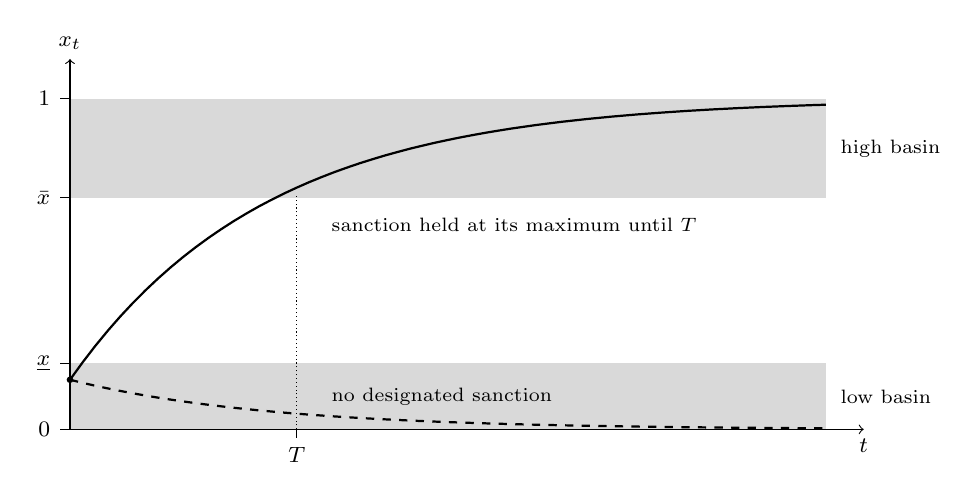
\begin{tikzpicture}[x=0.32cm,y=4.2cm,font=\footnotesize]
\fill[black!15] (0,0.7) rectangle (30,1);
\fill[black!15] (0,0) rectangle (30,0.2);
\draw[->] (0,0) -- (31.5,0) node[below] {$t$};
\draw[->] (0,0) -- (0,1.12) node[above] {$x_t$};
\foreach \y/\l in {0/0,0.2/\underline{x},0.7/\bar x,1/1} \draw (0,\y) -- (-0.4,\y) node[left] {$\l$};
\draw (9,0) -- (9,-0.025) node[below] {$T$};
\draw[densely dotted] (9,0) -- (9,0.71);
\draw[thick,domain=0:30,samples=61] plot (\x,{1-0.85*0.88^\x});
\draw[thick,dashed,domain=0:30,samples=61] plot (\x,{0.15*0.88^\x});
\fill (0,0.15) circle (1.2pt);
\node[anchor=west,font=\scriptsize] at (10,0.62) {sanction held at its maximum until $T$};
\node[anchor=west,font=\scriptsize] at (10,0.1) {no designated sanction};
\node[anchor=west,font=\scriptsize] at (30.2,0.85) {high basin};
\node[anchor=west,font=\scriptsize] at (30.2,0.1) {low basin};
\end{tikzpicture}
\caption{The path of the political state from the same start $x_0$ in the low basin
$[0,\underline x]$, under the partial-adjustment law. Dashed: without a designated
sanction the state stays in the low basin, where realized sanctions do not rise.
Solid: a sanction held at its maximum until date $T$ carries the state into the
high basin $[\bar x,1]$, after which equilibrium play keeps it there and the
sanction never falls (\Cref{prop:lock-in}).}
\label{fig:state-path}
\end{figure}

% @econ-contract paragraph
% id: DISC_BLUFFING
% role: Relate the designated sanction to bluffing under incomplete information (the author, 2026-10-17: "cite other paper's bluffing result ... they actually turn the bluffing to be true, and that caused the persist sanctions under this model"): a sanction imposed as a bluff, or to call one, and held long enough moves the state into the high basin, where continuing it is equilibrium play.
% depends_on: DISC_DESIGNATED_SANCTION
% handoff: Relief in practice.
% exact_ref: bib:Spaniel2015#pp=735-736,739
% source_role: bib:Spaniel2015#pp=735-736,739 => Under uncertainty about leader strength, weaker target leaders have incentives to bluff strength by continuing a crisis, and foreign powers sometimes call potential bluffs by implementing sanctions (read 2026-10-17 from the PDF); the bluffing result the paragraph builds on, not support for a result of this paper.
% exact_ref: bib:Brekhov2022#p=77
% source_role: bib:Brekhov2022#p=77 => Analyses targets' incentives to bluff under sanction (and reward) regimes in a repeated interaction with asymmetric information (read 2026-10-17 from the PDF); positioning only.
% exact_ref: tex-label:prop:lock-in
% support_status: VERIFIED
% status: PROPOSED
% @end-econ-contract
\central{Sanctions that begin as bluffs can become self-sustaining under equilibrium
play.} Under incomplete information, imposing sanctions can serve as a bluff or as a way
to call an opponent's bluff. In \citet[pp.~735--736]{Spaniel2015}, weaker target leaders
have ``incentives to bluff strength'' by continuing a crisis, and foreign powers respond
``by sometimes conceding and sometimes calling potential bluffs by implementing
sanctions''; \citet[p.~77]{Brekhov2022} analyzes target incentives to bluff under
sanctions. In those models, information revealed during the crisis determines subsequent
outcomes. Here, sanctions also shift the political state. A sanction imposed as a
bluff---or to call an opponent's bluff---and maintained for a sufficient duration acts as
a designated sanction in the sense defined above: it moves the state into the high basin,
where continued sanctioning is prescribed by equilibrium play. The bluff then becomes
self-fulfilling, and sanctions persist without any beliefs to revise.

\subsection{Real-world sanctions relief}
\label{sec:discussion:relief}
\label{sec:discussion:evidence}

% @econ-contract paragraph
% id: DISC_THREE_QUESTIONS
% role: Separate preference for relief, belief that it will be honoured, and its usability, and state the participation result (prop:relief-participation) at its scope, in words, as the model's answer to the first question.
% depends_on: DISC_BLUFFING
% handoff: Credibility of relief.
% merged_from: DISC_PARTICIPATION
% exact_ref: tex-label:prop:relief-participation
% support_status: NOT_APPLICABLE
% status: PROPOSED
% @end-econ-contract
\central{A natural application of the model is to proposals for sanctions relief, which raise
three related but distinct questions; the model's incentive comparisons speak to the
first.}\footnote{The participation
result is proved in \Cref{app:proofs:branch} of the Online Appendix; the economy
at which a temporary suspension of sanctions benefits a non-compliant target is recorded in the
formal supplement.}
Would policymakers prefer the arrangement and expect it to be honored, and would nominal
relief restore the economic activity it is intended to enable? On the first question,
consider a temporary suspension of sanctions followed by any equilibrium where the target
maintains full non-compliance, such as the constructed equilibrium. Under the
entrenchment condition and a sender response at full non-compliance that does not
decrease with the state, the change in incumbent payoffs does not support any date-zero
side payment between governments that would make the shock mutually acceptable. That
neither incumbent gains from such a shock follows jointly from three conditions: the
sender's positive marginal return to sanctioning a non-compliant target, the property
that compliance does not increase the sender's payoff at zero sanctions, and the
entrenchment condition. For an economy failing the entrenchment condition, a temporary
suspension of sanctions benefits a target that still does not comply.

% @econ-contract paragraph
% id: DISC_CREDIBILITY
% role: Tie the credibility of relief to commitment technologies and to lock-in, with the relief credibility point.
% depends_on: DISC_THREE_QUESTIONS
% handoff: Rival accounts of non-relief.
% exact_ref: bib:Powell2012#scope=paper
% source_role: bib:Powell2012#scope=paper => Already-cited source that singles out a costlessly reversible concession as least credible; it does not model this paper's state channel.
% support_status: UNVERIFIED
% status: PROPOSED
% @end-econ-contract
\central{The second question---whether relief will be honored---depends on commitment
technologies.} Lock-in depends on the initial state, and within a high basin resumed
equilibrium play generates no endogenous exit under the set and level conditions of
\Cref{prop:lock-in}. Expiry dates, review clauses, and other commitment technologies
operate by altering the strategic environment. Relief poses the hardest test for such
mechanisms. Relief that is reversible at no direct cost is the type that
\citet[p.~627]{Powell2012} identifies as least credible. In recent bargaining models of
war, the reliability of an agreement remains a parameter \citep{Ruggiero2026}. A full
model of relief institutions would need to specify, as separate primitives, who can
commit, who holds veto power, how private actors respond, and how these choices alter the
continuation game.

% @econ-contract paragraph
% id: DISC_RIVAL_ACCOUNTS
% role: Place rival accounts of non-relief without dismissing them as non-optimising (repair C6).
% depends_on: DISC_CREDIBILITY
% handoff: What the case material supports.
% exact_ref: bib:HalcoussisKaempferLowenberg2021#scope=paper
% source_role: bib:HalcoussisKaempferLowenberg2021#scope=paper => Already-cited legislative-cost account of sanction persistence; cited as an alternative, not as support for this model.
% support_status: UNVERIFIED
% status: PROPOSED
% @end-econ-contract
\central{Commitment problems are one explanation for persistent non-relief among
several; the model isolates a distinct mechanism.} In this mechanism, continued sanctions
can be optimal because of the state that sanctions have built, provided that the sender
values that target-side state and the entrenchment condition holds. Sanctions can be
optimal even if they are re-optimized every period and a lower sanction level is
feasible. Legislative constraints \citep{HalcoussisKaempferLowenberg2021}, administrative
persistence, and reputational incentives offer alternative explanations. Political or
reputational costs can themselves be incorporated into an optimizing decision
framework.

% @econ-contract paragraph
% id: DISC_PREDICTIONS
% role: State the two observable responses the classification separates, as model implications, not validation.
% depends_on: DISC_RIVAL_ACCOUNTS
% handoff: The case material.
% exact_ref: tex-label:thm:four-cells
% support_status: VERIFIED
% status: PROPOSED
% @end-econ-contract
\central{Comparisons across constructed equilibria distinguish two observable responses
to a single sanctions regime: greater compliance and deeper entrenchment.}\footnote{The
model's predictions are collected in \Cref{app:moved-ah} of the Online Appendix,
and the case sources' discussion of evasion and enforcement in
\Cref{app:moved-ad}.} Greater
compliance arises when the target's forward-looking incentive is weak and a
forward-looking sender raises the cost of relief; deeper entrenchment arises when that
incentive is strong and a forward-looking sender raises the steady-state level.

% @econ-contract paragraph
% id: DISC_CASE_MATERIAL
% role: Use the already-cited case material as motivation for the mechanism, with the Sender's stake kept as a maintained restriction.
% depends_on: DISC_PREDICTIONS
% handoff: The relief cases.
% exact_ref: bib:HaggardNoland2017#scope=paper
% source_role: bib:HaggardNoland2017#scope=paper => Already-cited account of an authoritarian target passing sanction costs to citizens; motivates the mechanism, does not identify any parameter.
% exact_ref: bib:UNPanelDPRK2024#scope=paper
% source_role: bib:UNPanelDPRK2024#scope=paper => Already-cited report of tighter control under sanctions; motivation only.
% support_status: UNVERIFIED
% status: PROPOSED
% @end-econ-contract
\central{North Korea, a context in which this feedback mechanism may be salient, helps
motivate the analysis.} \citet{HaggardNoland2017} describe an authoritarian target able
to pass sanction costs onto its citizens and a leadership reluctant to weaken its control
over foreign economic activity; in the model's terms, these correspond to low sanction
pain and a high valuation of the state---the two sides of the entrenchment condition. A
United Nations Panel of Experts report documents tighter economic, social, and political
controls and more centralized economic management under sanctions
\citep{UNPanelDPRK2024}. These same sources document evasion, enforcement, and
coordination challenges, which can coexist with the political-state feedback
mechanism.

% @econ-contract paragraph
% id: DISC_CASE_RELIEF
% role: Use the Iranian and Russian relief material (note N134, promoted 2026-10-02) to separate acceptability, credibility and delivery of relief, as motivation only.
% depends_on: DISC_CASE_MATERIAL
% handoff: The limits of the equilibrium interpretation.
% exact_ref: tex-label:sec:discussion:relief
% exact_ref: bib:BajoghliNasrSalehiIsfahaniVaez2024#pp=115-116,121-123
% source_role: bib:BajoghliNasrSalehiIsfahaniVaez2024#pp=115-116,121-123 => The authors' account (read 2026-10-02) that the prospect of lifting brought Iran to the 2015 agreement while rollback was slow, could be blocked or reimposed through Congress, and was made immaterial by remaining financial sanctions; motivation for separating the three relief questions, not a test of the model.
% exact_ref: bib:SnegovayaFentonDolbaiaBergmann2025#pp=26,31-32
% source_role: bib:SnegovayaFentonDolbaiaBergmann2025#pp=26,31-32 => The report's description (read 2026-10-02) of Russian businesses that thrive under isolation and fear returning competition, against firms that would gain from partial relief, with its scenario assumptions; heterogeneous interests, projections rather than observed outcomes.
% support_status: UNVERIFIED
% status: PROPOSED
% @end-econ-contract
\central{Iran and Russia illustrate all three questions raised above.} According to
\citet[pp.~115--116]{BajoghliNasrSalehiIsfahaniVaez2024}, the prospect of earlier
sanctions being lifted---not the threat of additional sanctions---brought Iran to the 2015
agreement. Yet the rollback was gradual and required political support at multiple levels
of the United States government. Congress, which is often involved in delisting
decisions, could impose additional hurdles or reimpose the same sanctions under another
pretext, and sanctions remaining on Iran's financial and banking system made the lifting
of others immaterial (pp.~121--123). Accepting relief, expecting it to be honored, and
being able to benefit from it are therefore distinct margins. In Russia, businesses that
have thrived under reduced competition fear the return of Western competitors, while
import- and export-dependent firms could gain from partial sanctions relief
\citep[pp.~31--32]{SnegovayaFentonDolbaiaBergmann2025}. The report's scenarios are
projections from 2025 (p.~26). This heterogeneity is what the political state variable
summarizes.

\subsection{Scope and limitations}
\label{sec:discussion:scope}

% @econ-contract paragraph
% id: DISC_SCOPE
% role: State the mechanism the model isolates and the object of its theorems for a specified instrument and compliance demand; effectiveness judged against a sender's objectives; how the class specializes to other coercive systems.
% depends_on: DISC_CASE_RELIEF
% handoff: The equilibrium concept and the results that reach beyond the constructed equilibria (repair C2).
% exact_ref: bib:GAO2025RussiaSanctions#pp=14
% source_role: bib:GAO2025RussiaSanctions#pp=14 => The report's three categories of objectives (read 2026-10-02); names the objectives against which effectiveness is judged, supports no model result.
% support_status: NOT_APPLICABLE
% status: PROPOSED
% @end-econ-contract
\central{We have deliberately isolated one public-choice mechanism behind persistent sanctions:
sanctions strengthen the target-side constituency that supports their continuation, and
both governments value that constituency.} Within the class, compliance affects the
sender by reducing its incentive to sanction. Given a coercive instrument and a
compliance demand, the theorems characterize how equilibrium play evolves from the
political state that sanctions---once imposed---have altered. Effectiveness, by contrast,
is measured against a sender's objectives, which the U.S. Government Accountability
Office identifies for U.S. measures on Russia as economic pressure, inhibition of the war
effort, and accountability \citep[p.~14]{GAO2025RussiaSanctions}. The mathematical
structure of the class can be adapted to other coercive systems. Doing so requires
mapping their actions, constituency effects, and payoff signs into the class structure,
including analogues of each government's stake in the state and of the entrenchment
condition.

% @econ-contract paragraph
% id: MODEL_EQUILIBRIUM_SCOPE
% role: How existence is obtained (by construction on invariant sets of value functions), and the concept against strong stationary Stackelberg and history-dependent equilibria (moved from Section 2.4, 2026-10-16, structure plan S4).
% depends_on: DISC_SCOPE
% handoff: The objects solved jointly and the results beyond the constructed equilibria.
% exact_ref: tex-label:thm:existence
% exact_ref: bib:HeLiuChen2025#scope=paper
% source_role: bib:HeLiuChen2025#scope=paper => Already-cited dynamic feedback Stackelberg existence and computation antecedent (restored 2026-10-02 after the rebuild dropped it); positions the joint-iteration existence route, does not prove it.
% exact_ref: bib:LiSojoudiTomlinFridovichKeil2024#scope=paper
% source_role: bib:LiSojoudiTomlinFridovichKeil2024#scope=paper => Already-cited feedback Stackelberg computation antecedent (restored 2026-10-02 after the rebuild dropped it); positioning only.
% exact_ref: tex-label:prop:history-deviations
% support_status: VERIFIED
% status: PROPOSED
% @end-econ-contract
\central{Existence is established by construction, and each construction pins down its
equilibrium only within the sets of value functions it employs.} Where the results
construct a value function, it is the unique fixed point of its Bellman operator defined
over an explicitly stated \emph{invariant set of value functions}: a closed set with
stated bounds on the level and slope of each member (and on
curvature for the sender), which the operator maps into itself. \Cref{sec:results} constructs
equilibria over the full class of economies. A general existence argument---based on
joint contraction of both Bellman equations when the coupling between them is
sufficiently weak---follows in the spirit of \citet{StokeyLucas1989} and of broader
research on the existence and computation of dynamic feedback Stackelberg equilibria
\citep{HeLiuChen2025,LiSojoudiTomlinFridovichKeil2024}.

\central{Two comparisons delineate the scope of the equilibrium concept: with the
stationary strong Stackelberg equilibrium, and with history-dependent strategies.}
First, target optimality in $\mathcal E$ is pointwise: at each state, the target
maximizes the right-hand side of \eqref{eq:T-bellman}, taking continuation values as
given. In a stationary strong Stackelberg equilibrium, by contrast, the leader selects an
entire policy function and anticipates that the follower re-optimizes after every policy
deviation; the two concepts need not coincide \citep{Bucarey2023,KudoAkimoto2026}. The
equilibrium concept is time-consistent because both governments re-optimize at every
state. Second, against any equilibrium in $\mathcal E$, no pure strategy conditioned on
the entire history outperforms the equilibrium's own play, from any initial state
and---for the sender---after any observed compliance level on or off the equilibrium
path.

% @econ-contract paragraph
% id: DISC_EQUILIBRIUM_LIMITS
% role: State the equilibrium notion, the objects it solves jointly, and the two results that reach beyond the constructed equilibria (repair C2).
% depends_on: MODEL_EQUILIBRIUM_SCOPE
% handoff: Levels of generality.
% merged_from: DISC_ENDOGENOUS
% exact_ref: tex-label:prop:security
% note: 2026-10-16 (structure plan S4): the Markov sentence is in Section 2.4 and the minmax and uniqueness results in Section 3.4; this paragraph points there.
% support_status: VERIFIED
% status: PROPOSED
% @end-econ-contract
\central{Within each equilibrium, the target's compliance rule, the sender's sanction
rule, both value functions, both feedback policies, and the political-state trajectory
are solved jointly.} In the interest-group polity, the pressure levels of competing
groups also constitute a Nash equilibrium of the political contest. Two results extend
beyond the constructed equilibria under the strong entrenchment condition: the target's
minmax payoff bound and the uniqueness of full non-compliance among non-decreasing
sanction rules (\Cref{sec:results:security}).

% @econ-contract paragraph
% id: DISC_GENERALITY_LEVELS
% role: Separate results about every equilibrium satisfying stated conditions, results derived from primitives on the class, and results established at example economies, citing main-text results only.
% depends_on: DISC_EQUILIBRIUM_LIMITS
% handoff: Open extensions.
% exact_ref: tex-label:prop:certified-equilibria
% support_status: VERIFIED
% status: PROPOSED
% @end-econ-contract
\central{The results operate at three levels of generality.} First, some apply to every
equilibrium satisfying stated conditions: lock-in (\Cref{prop:lock-in}) applies to every
equilibrium meeting its basin conditions and, for entry, its transition conditions; the
fixed-target-policy comparison (\Cref{thm:dominance}) applies to every non-decreasing
sender value at every state, and thus to every equilibrium containing one; the premium bound
of \Cref{sec:results:wedge} applies to every equilibrium with a non-increasing target
policy, for economies in the class with an upper bound on the substitution rate at which
larger concessions are never worth more to the sender at zero sanctions; and the minmax
bound applies to every equilibrium in $\mathcal E$. Second, the myopic-benchmark
comparison (\Cref{thm:regime-separation}), the four-case characterization
(\Cref{thm:four-cells}), and the threshold result (\Cref{prop:collapse-threshold}) derive
equilibrium properties and dynamics from inequalities across primitives over the class, and
greater target patience preserves the full-non-compliance equilibrium that exists at a
lower discount factor (\Cref{prop:patience-existence}). The welfare results of
\Cref{sec:welfare} hold across the class, as do the rescaling property and the planner
optimality condition for any representation and any bounded welfare flow. Third, some
results are established via example economies, which demonstrate that hypotheses can be
satisfied or bounds attained: the welfare loss in one interest-group polity
(\Cref{sec:welfare:efficiency}), the attainment of the premium bound
(\Cref{sec:results:wedge}), and economies satisfying the lock-in conditions
(\Cref{app:persistence:reading} of the Online Appendix).

% @econ-contract paragraph
% id: DISC_OPEN
% role: Name the extensions and the measurement requirements for empirical work.
% depends_on: DISC_GENERALITY_LEVELS
% handoff: The conclusion.
% exact_ref: bib:AttiaGrauvogel2023#scope=paper
% source_role: bib:AttiaGrauvogel2023#scope=paper => Already-cited exploratory association between institutional clauses and termination; not a causal estimate and not support for a model result.
% support_status: UNVERIFIED
% status: PROPOSED
% @end-econ-contract
\central{Two broad kinds of extensions build on these results: empirical measurement of
the political state and its associated payoff terms, and richer theoretical models of
the state and of relief institutions.} Disciplining estimates of the political-state
transition and the payoff terms governing basin entry would require empirical measures
that separate the political state from aggregate income, and distinguish within-target
adjustment from selection across surviving episodes. Theoretical extensions could
incorporate multidimensional political states, stochastic shock duration,
forward-looking investment by groups in their own future power
\citep{AcemogluRobinson2008}, or explicit relief and commitment technologies. The last of
these could alter entry into or create exit from the high basin, and
\citet{AttiaGrauvogel2023} document exploratory empirical associations between such
provisions and sanction termination. A fully optimal relief policy would require explicit
institutional instruments and commitment constraints. A symmetric framework in which both
governments directly move the state---of the kind \citet{Powell2013} calls for---would
embed compliance directly into the transition law and require rederiving the argument
that compliance reduces the sender's incentive to sanction.

% @econ-contract include
% id: INCLUDE_CONCLUSION
% file: main_sections/06_conclusion.tex
% section_contract: CONCLUSION_ANSWER
% role: Answer the question at its proved scope and state its limits.
% question_answered: What was established, and where does it stop?
% required_inputs: All result sections.
% output_handoff: None.
% claim_ceiling: The master plan's ceiling; no policy prescription.
% status: HUMAN_CONFIRMED
% @end-econ-contract
% @econ-contract section
% id: CONCLUSION_ANSWER
% role: Answer the question at its proved scope: the mechanism and answer first; who decides accommodation, who decides intensity; what the reach results add; the persistence and welfare limits.
% question_answered: What did the paper establish, and where does it stop?
% required_inputs: RESULTS_HORIZONS, WELFARE_BOUNDARY, DISCUSSION_INTERPRETATION.
% output_handoff: None.
% claim_ceiling: The master plan's ceiling; no policy prescription.
% exclusions: A theorem list; new claims.
% exact_ref: tex-label:sec:conclusion
% support_status: VERIFIED
% status: HUMAN_CONFIRMED
% human_confirmed_at: 2026-10-01
% decision_ref: suggestions/2026-10-01-manuscript-rebuild/01_STRUCTURE_PROPOSAL.md#author-decisions-recorded
% confirmation_scope: Section role and claim ceiling.
% reopen_if: A principal result or the claim ceiling changes.
% amended_at: 2026-10-12 (opens on the dual-basin illustration and states its limits; decision_ref: suggestions/2026-10-10-jet-submission/DECISIONS.md#framing-2026-10-12); 2026-10-13 (argument plan: mechanism and answer first, then the dual-basin illustration with its limits, the reach results, welfare and lock-in, and a closing 'so what / now what' paragraph; decision_ref: suggestions/2026-10-10-jet-submission/exposition-2026-10-13/ARGUMENT_PLAN.md); 2026-10-15 (the dual-basin illustration dropped from the main text for now, on the author's word); 2026-10-19 (coauthor wording review: wording of the coauthor's line-by-line revision applied where not wrong; sender/target in lower case; non-compliance for defiance; decision_ref: suggestions/2026-10-10-jet-submission/DECISIONS.md#coauthor-wording-review-2026-10-19); 2026-10-20 (humanizer pass: dashes replaced by commas, parentheses or colons; plain wording; meaning unchanged; decision_ref: suggestions/2026-10-10-jet-submission/DECISIONS.md#humanizer-pass-2026-10-20)
% @end-econ-contract
\section{Conclusion}
\label{sec:conclusion}

% @econ-contract paragraph
% id: CONCLUSION_ROLES
% role: Open with the mechanism and the answer on the class (the myopic benchmark ends sanctions, forward-looking governments sustain them; the Target's patience decides relief against defiance), then the Sender's role and the same-policy comparison with its hypothesis (repair C4). Moved first (argument plan, 2026-10-13); reordered on the layout decisions of 2026-10-16.
% depends_on: CONCLUSION_ANSWER
% handoff: The reach results.
% exact_ref: tex-label:prop:myopic-benchmark
% exact_ref: tex-label:thm:regime-separation
% exact_ref: tex-label:thm:four-cells
% exact_ref: tex-label:thm:dominance
% support_status: VERIFIED
% status: PROPOSED
% @end-econ-contract
\central{Economic sanctions can persist because they strengthen the domestic political
interests that support their continuation.} Without foresight they unravel: in the
myopic benchmark, the target accommodates and the political state erodes over time. In
the equilibria constructed over the class of economies, when both governments value the
political state and are forward-looking, the target maintains non-compliance, sanctions
persist indefinitely, and the political state converges to a positive steady-state
level. The target's patience determines whether relief or non-compliance prevails;
whether the sender is forward-looking shapes the compliance threshold for relief or the
intensity of sanctions under non-compliance. These comparisons hold all non-discount
primitives fixed. For a fixed target policy, a non-decreasing sender continuation value
weakly increases the largest of the optimal sanctions relative to the myopic best response. Under
interiority, the constructed equilibria exhibit a strictly positive foresight premium
relative to the myopic best response, with a closed-form lower bound.

% @econ-contract paragraph
% id: CONCLUSION_REACH
% role: Summarize the reach results: patience, like the Target's other parameters, can change whether full defiance is an equilibrium; result names in place of condition lists (argument plan, 2026-10-13).
% depends_on: CONCLUSION_ROLES
% handoff: The welfare findings and lock-in.
% exact_ref: tex-label:prop:security
% exact_ref: tex-label:prop:collapse-threshold
% support_status: VERIFIED
% status: PROPOSED
% @end-econ-contract
\central{Beyond the constructed equilibria, patience, like all other target
parameters, shapes whether full non-compliance is supportable as an equilibrium.} When
the sender's response and the target's value under full non-compliance do not decrease
with the state, greater target patience preserves the full-non-compliance equilibrium.
Under the strong entrenchment condition, the target guarantees itself a minmax payoff
against every pure sanction strategy, bounding its payoff in every equilibrium from
below; and across the class, every equilibrium with a non-decreasing sanction rule
exhibits full non-compliance. In the special case of \Cref{prop:collapse-threshold}, a
full-non-compliance equilibrium exists if and only if the target's discount factor is at
least a threshold value.

% @econ-contract paragraph
% id: CONCLUSION_LIMITS
% role: State the welfare findings, then lock-in and persistence without hysteresis, naming prop:lock-in instead of listing its conditions (argument plan, 2026-10-13).
% depends_on: CONCLUSION_REACH
% handoff: So what and now what.
% exact_ref: tex-label:sec:welfare
% exact_ref: tex-label:prop:lock-in
% support_status: VERIFIED
% status: PROPOSED
% @end-econ-contract
\central{Persistent sanctions can be socially costly, and the game alone does not
determine their welfare ranking.} Across the class, two interest-group representations
of the same government payoffs rank the constructed equilibria in opposite orders, and
under compliance neutrality one makes persistent play socially optimal. For an example
economy with one explicit interest-group polity, equilibrium sanctions remain at their
maximum level and generate welfare losses.

The political state can also lock in sanctions. Where an equilibrium and a high-state
interval satisfy the conditions of \Cref{prop:lock-in}, a state entering the interval
remains there under equilibrium play and sanctions never decline. When full sanctions
raise every state below the basin, a sufficiently long temporary shock can produce a
durable outcome. Persistence can also arise without hysteresis. Where the explicit
Lipschitz constant derived for the constructed equilibrium's law of motion is strictly
below one, a temporary shock has no permanent asymptotic effect.

% @econ-contract paragraph
% id: CONCLUSION_SO_WHAT
% role: Say what the results mean (persistence need not reveal failed bargaining or misperception; with information complete, the levers act on the political state and the governments' incentives, not on beliefs) and what would discipline the channel (measurement, sec:discussion:scope), with no prescription; close on the paper's answer.
% depends_on: CONCLUSION_LIMITS
% handoff: None.
% origin: argument plan item 10 (2026-10-13); the closing sentence moved here from CONCLUSION_LIMITS.
% exact_ref: tex-label:sec:discussion:scope
% exact_ref: tex-label:sec:discussion:misperception
% support_status: VERIFIED
% status: PROPOSED
% @end-econ-contract
\central{Persistent sanctions therefore need not reflect failed bargaining or
misperception.} Within the model, they can be the optimal choice of governments that
value the political state that sanctions themselves have built. With complete
information, the levers that end sanctions operate through the political state and
government incentives, not through beliefs (\Cref{sec:discussion:misperception} of the
Online Appendix). Whether this channel operates in a given episode is an empirical
question: measurements that separate the political state from aggregate income would
discipline estimates of its transition and of the payoff terms governing basin entry
(\Cref{sec:discussion:scope}). \central{Optimizing governments can thus perpetuate and
lock in sanctions through the political state that sanctions generate; patience and
other economic features determine whether this occurs.}

% @econ-contract include
% id: INCLUDE_DECLARATIONS
% file: main_sections/07_declarations.tex
% section_contract: DECLARATIONS_STATEMENTS
% role: Carry the required author declarations.
% question_answered: Competing interests, funding, contributions, AI use, data availability.
% required_inputs: Author records.
% output_handoff: None.
% claim_ceiling: Declarations only; no scientific claim.
% status: HUMAN_CONFIRMED
% @end-econ-contract
% @econ-contract section
% id: DECLARATIONS_STATEMENTS
% role: Carry the required author declarations.
% question_answered: Competing interests, funding, contributions, AI use, data availability.
% required_inputs: Author records.
% output_handoff: None.
% claim_ceiling: Declarations only; no scientific claim.
% exclusions: Any scientific claim.
% support_status: NOT_APPLICABLE
% status: HUMAN_CONFIRMED
% human_confirmed_at: 2026-10-01
% decision_ref: suggestions/2026-10-01-manuscript-rebuild/01_STRUCTURE_PROPOSAL.md#author-decisions-recorded
% confirmation_scope: Section role only; the declarations' content is the author's.
% reopen_if: Journal requirements or the author's declarations change.
% amended_at: 2026-10-19 (data availability names the release v1.30-submission; decision_ref: suggestions/2026-10-10-jet-submission/DECISIONS.md#submission-release-2026-10-19); 2026-10-20 (the repository link; decision_ref: suggestions/2026-10-10-jet-submission/DECISIONS.md#repository-link-and-acemoglu-notes-2026-10-20); 2026-10-20 (the release is public at the new repository; decision_ref: suggestions/2026-10-10-jet-submission/DECISIONS.md#public-repository-2026-10-20); 2026-10-21 (Elsevier layout: the generative-AI statement is its own section, titled as the Guide requires, last before the references, wording otherwise unchanged; funding in the Guide's sentence; data availability without the internal script name, citing the release; decision_ref: suggestions/2026-10-10-jet-submission/DECISIONS.md#jet-submission-package-2026-10-21)
% @end-econ-contract
\section*{Declarations}

% Coauthors' confirmation of no competing interests: received (the author, 2026-10-21).
\paragraph{Declaration of competing interest.} The authors declare no
competing financial interests or personal relationships that could have
influenced the work reported in this paper.

\paragraph{Funding.} This research did not receive any specific grant from funding
agencies in the public, commercial, or not-for-profit sectors.

\paragraph{CRediT author statement.} Xiaofeng Gong:
Conceptualization, Formal analysis, Methodology, Software, Validation,
Visualization, Writing -- original draft, and Writing -- review and
editing. Yuechuan Zhao: Conceptualization, and Writing -- review and
editing. Chunping Zhong: Conceptualization, and Writing -- review and
editing.

\paragraph{Data availability.} No empirical data were used. The Lean~4 formalization
that machine-checks the core results of this paper, as mapped in the formal supplement, is
public as the release \texttt{v1.30-submission} at
\url{https://github.com/qidaolake/political-entrenchment-sanctions-lean}
\citep{GongLean2026}, with the manuscript, the Online Appendix and the formal supplement
attached to it. Its source archive accompanies this submission as supplementary material.
A deposit with a DOI will accompany publication.

\paragraph{Formalization methods.} The Lean~4 development was written with
assistant-generated suggestions for proof steps and lemma search. The
selection of the statements to formalize, the economic interpretation of
every formal statement, and the correspondence map between the manuscript
and the declarations were made and reviewed by the authors, and the Lean~4
kernel independently checks every proof term in the archived release. A
kernel check certifies a formal statement; it does not certify that an
informal economic sentence translates that statement faithfully, which is
why the correspondence is recorded as a separately reviewed map in the
formal supplement.


% ---------------------------------------------------------------------
% COMBINED mode only: inline the appendix so that a single PDF carries
% both the manuscript and the appendix under one bibliography.
% ---------------------------------------------------------------------


\ifdefined\COMBINEDAPPENDIX
% @econ-contract include
% id: INCLUDE_APPENDIX_BODY
% file: sanctions_appendix_body.tex
% section_contract: APPENDIX_INDEX
% role: Inline the appendix in the combined build only; the split build cross-references the standalone appendix.
% question_answered: Where are the exact statements, proofs, constructed economies and the formalization map?
% required_inputs: All main sections.
% output_handoff: None.
% claim_ceiling: Exact statements and proofs of the results the main text states; no further claim.
% status: HUMAN_CONFIRMED
% @end-econ-contract
  % @econ-contract section
% id: APPENDIX_INDEX
% role: Order the appendix in three parts: general results for abstract payoffs and transitions in the class (conditions and component statements, proofs, persistence and lock-in, existence, discharge routes, supporting results, further statements); examples (parametric families and the roster, numerical economies, closed-form constants, the interest-group example); the literature (the author's decision, 2026-10-20); within each part, what the main text needs comes before derivative and supplementary material (2026-10-20).
% question_answered: Where is each exact statement and proof?
% required_inputs: The main sections.
% output_handoff: None.
% claim_ceiling: Exact statements and proofs of results the main text states; machine-checked statements as recorded in the formalization map.
% exclusions: New claims not stated or summarised in the main text.
% exact_ref: file:appendix_sections/07_formalization_map.tex#label=app:formalization
% source_role: file:appendix_sections/07_formalization_map.tex#label=app:formalization => The formal supplement's formalization map, which records the Lean declaration behind each statement; it establishes formal derivation, not economic correspondence.
% support_status: VERIFIED
% status: HUMAN_CONFIRMED
% human_confirmed_at: 2026-10-01
% decision_ref: suggestions/2026-10-01-manuscript-rebuild/01_STRUCTURE_PROPOSAL.md#author-decisions-recorded
% confirmation_scope: Appendix role and the D1 moves.
% amended_at: 2026-10-20 (three parts, general results and examples separated, on the author's "see whether we can have a generalized form abstract functional form appendix versus a numerical example appendix please, make it more organized"; decision_ref: suggestions/2026-10-10-jet-submission/DECISIONS.md#appendix-in-three-parts-and-the-one-sided-cases-paragraph-2026-10-20); 2026-10-20 (within each part, what the main text needs before derivative material; decision_ref: suggestions/2026-10-10-jet-submission/DECISIONS.md#appendix-needed-versus-derivative-2026-10-20); 2026-10-20 (proof maps open Part I; decision_ref: suggestions/2026-10-10-jet-submission/DECISIONS.md#proof-maps-and-reading-the-lean-statements-2026-10-20)
% reopen_if: A section moves between the main text and the appendix.
% @end-econ-contract
% =====================================================================
%  SHARED APPENDIX INDEX  --  sanctions_appendix_body.tex
%
%  This file is NOT a document.  It is \input by BOTH:
%     sanctions_jet_appendix.tex   -> standalone appendix PDF
%     sanctions_jet_draft.tex      -> only in COMBINED mode
%  so the two builds cannot diverge.  It begins at \appendix, inputs the
%  ordered files under appendix_sections/, and ends before the bibliography,
%  which each root supplies for itself.
% =====================================================================

\appendix

% Everything below is an appendix, so cleveref must call it one.  Without
% these two lines \Cref{app:closedforms} typesets as "Section C" -- which,
% now that the appendix is a separate document, names a section the
% manuscript does not contain.  (The \crefnames are in sanctions_preamble.tex.)
\crefalias{section}{appendix}
\crefalias{subsection}{subappendix}
\crefalias{subsubsection}{subappendix}

% Ordered appendix-section index; section bodies live in appendix_sections/.
\section*{How to read this appendix}

\paragraph{Where the main text's proofs are.} Each subsection of the main text
opens with a footnote that points here; the map collects those pointers.
\begin{itemize}
\item Section~\ref{sec:model} (the model): the bounds of the class and the precise conditions
in panel~A0 of \Cref{app:proofs:placable} and in
\Cref{sec:moved-main-2026-10-13:conditions}; the closed-form constants in
\Cref{app:closedforms}; the parametric examples in \Cref{sec:model:examples}; the
example economies in \Cref{app:witness,app:fourgroup}, and the numerical ones, among them the dual-basin
economy, in \Cref{sec:moved-main-2026-10-15,app:dual-basin-economy}; existence in \Cref{app:existencemachinery}.
\item Section~\ref{sec:model:myopic} (the myopic benchmark) and Section~\ref{sec:results:main} (foresight against it):
panel~F of \Cref{app:proofs:placable}; the component statements in
\Cref{sec:moved-main-2026-10-13:components}.
\item Section~\ref{sec:results:wedge} (the target's and the sender's parts): \Cref{app:proofs:branch} and
\Cref{app:proof-dominance}; the strict comparison in
\Cref{sec:moved-main-2026-10-13:strict}.
\item Section~\ref{sec:results:lockin} (lock-in): \Cref{app:persistence}; the low basin in
\Cref{thm:lowbasin}; an equilibrium with both basins in \Cref{app:dual-basin-economy}.
\item Section~\ref{sec:results:patience} (patience): \Cref{app:proofs:threshold,app:proofs:scope}, and
the general conditions in \Cref{sec:moved-main-2026-10-13:bracket}.
\item The end of Section~\ref{sec:results:patience} (minmax and uniqueness): the statements in
\Cref{sec:moved-main-2026-10-13:security}, proved in \Cref{app:proofs:scope}.
\item Section~\ref{sec:welfare} (welfare): the proofs in \Cref{app:proofs:welfare};
\Cref{app:fourgroup} and \Cref{sec:moved-main-2026-10-13:welfare} for the
interest-group polity and the family's microfoundations.
\item Section~\ref{sec:discussion:horizons} (one government forward-looking): the component statements in
\Cref{sec:moved-main-2026-10-13:components}, proved in \Cref{app:proofs:placable};
the welfare reversal across the four cases in \Cref{app:proofs:welfare}.
\item Section~\ref{sec:discussion} (discussion): \Cref{app:persistence,app:decomposition-path}.
\end{itemize}


\paragraph{How the appendix is organized.} The appendix has three parts, and each of
the two larger parts puts what the main text needs before derivative material.
Part~I holds the general results, which hold for abstract payoffs and transitions in the
class, with no functional form. What the main text needs comes first: maps of how the
results are proved (\Cref{app:proof-maps}); the conditions in
full and the component statements of the main results
(\Cref{sec:moved-main-2026-10-13}); the proofs (\Cref{app:proofs}), among them the
construction on the class under the lifting condition with its class-membership panel
(\Cref{app:proofs:placable}); persistence, temporary shocks and lock-in, with the low
basin, relief and the exit duration (\Cref{app:persistence}); and the two-channel
decomposition and the path of the state (\Cref{app:decomposition-path}). The derivative
and supplementary results follow: the existence machinery (\Cref{app:existencemachinery}),
the assumption-discharge routes (\Cref{app:dischargers}), the robustness and boundary
results (\Cref{app:supporting-results}) and further results on persistence and the long
run (\Cref{app:moved-ak}). Part~II holds the examples: the ones the main text uses, the
parametric families with the benchmark economy (\Cref{app:witness}), the numerical
example economies (\Cref{app:numerical-examples}) and the microfounded interest-group
example (\Cref{app:fourgroup}); then further example economies
(\Cref{app:further-examples}) and the closed-form constants of the parametric family
(\Cref{app:closedforms}). Part~III places the paper in the literature
(\Cref{app:literature}). The formalization map, which lists for every statement the
machine-checked declaration that proves it, is in the formal verification supplement.
Every cross-reference in the manuscript resolves into this document.

\section*{Notation and symbols}

This list collects the symbols used repeatedly in the manuscript and
appendix. Symbols confined to a single proof, proposition, or certificate
table are defined locally where they first appear.

\begin{longtable}{@{}p{0.25\textwidth}p{0.69\textwidth}@{}}
\toprule
Symbol & Meaning\\
\midrule
\endfirsthead
\toprule
Symbol & Meaning\\
\midrule
\endhead
$t;\ x_t,\ a_t,\ s_t$
& Date $t\in\mathbb N$; political state, target compliance, and sender
sanction at date $t$, each of the three taking values in $[0,1]$.\\
$\F(x,s)$
& General state-transition law. Conditions \textup{(F1)--(F5)} impose
continuity, monotonicity, diagonal fixed points, and strict adjustment
toward the current sanction.\\
$\delta$
& Adjustment rate in the partial-adjustment law
$\F(x,s)=(1-\delta)x+\delta s$.\\
$\beta_T,\beta_S$
& target and sender discount factors.\\
$\Ut,\Us$
& target and sender one-period government objectives.\\
$\Vt,\Vs$
& target and sender continuation-value functions.\\
$T_T,T_S$
& target and sender Bellman operators.\\
$\gamma_F$
& Optional inherited-state Lipschitz modulus of $\F$ at a fixed sanction.\\
$J_S(x,a,s;\Vs)$
& Dynamic sender objective
$\Us(x,a,s)+\beta_S\Vs(\F(x,s))$.\\
$\sigM$
& The sender's myopic best response.\\
$\sigDyn_{\Vs},\ \sigDynTop_{\Vs}$
& The sender's dynamic argmax and its greatest selection, the dynamic best
response, at continuation value $\Vs$.\\
$\alpha,\ \alphaM$
& Equilibrium target policy and the independently optimized myopic target
policy.\\
$\alpha_{V_T,V_S}$
& target argmax policy induced by a value pair in
$\mathcal C_T\times\mathcal C_S$.\\
$E,\ \mathcal E$
& A stationary feedback Stackelberg equilibrium
$E=(\Vt,\Vs,\alpha)$ and the set of all such equilibria.\\
$M=(\alphaM,\sigM)$
& Myopic equilibrium. This roman $M$ is distinct from the
bold row-Lipschitz matrix $\mathbf M$ below.\\
$(x_t^E,s_t^E),\ (x_t^M,s_t^M)$
& Realized state and sanction paths of the equilibrium and of the myopic
equilibrium from the common initial state $x_0$.\\
$\bar x_T,\bar x_S;\ \bar x;\ \basin$
& target and sender tipping thresholds; their joint pivot
$\bar x=\max\{\bar x_T,\bar x_S\}$; and the high basin
$\basin=[\bar x,1]$.\\
$\bar s$
& Sanction-floor parameter used to construct the flip sets.\\
$\mathcal C_T,\mathcal C_S$
& target and sender value sets.\\
$L_{S,x}^{\alpha},\ K_S$
& Composite sender stage-payoff state modulus and the resulting Lipschitz
constant of the sender's value set. The latter is distinct from the sans-serif
commercial-lobby label $\KSgroup$.\\
$m_S,\ c_\sigma$
& sender stage lower-slope level and strict-concavity modulus.\\
$\mathcal F_T(\bar s),\
  \mathcal F_S(\bar s;m_S)$
& target and sender upper flip sets used to derive the basin thresholds.\\
$x_S^0,\ x_S(a)$
& Static sender flip and the sender's per-action flip threshold.\\
$\mathbf M$
& Joint Bellman row-Lipschitz matrix with entries
$\beta_T,L_{TS},L_{ST},\beta_{S,\mathrm{row}}$.\\
$\rho(\mathbf M)$
& Spectral radius of the row-Lipschitz matrix.\\
$R(x),\ G(x)$
& Sanction rule of the equilibrium and closed-loop state-update map,
$R(x)=\sigDynTop_{\Vs}(x,\alpha(x))$ and $G(x)=\F(x,R(x))$.\\
$00,\,01,\,10,\,11$
& The four cases of one economy, target-first: the first index is $1$
when the target is forward-looking ($\beta_T>0$) and $0$ when it is myopic, the
second the same for the sender; $R^{ij}$, $L^{ij}$ and $a^{ij}$ are the
sanction rule, the limit of the political state and the target policy in case
$ij$ (\Cref{sec:four-regimes}).\\
$w_{\mathrm{lo}}$, $w_{\mathrm{hi}}$, $q$, $\bar Q$, $r_{\mathrm{lo}}$,
$r_{\mathrm{hi}}$, $k_{\mathrm{lo}}$, $k_{\mathrm{hi}}$, $u_{\mathrm{lo}}$,
$u_{\mathrm{hi}}$, $\sigma_x$, $\tau_x$
& The class's sender rates: state slope, sanction curvature, state--sanction
cross rate, substitution rate and marginal return to the first
unit of sanction, each as a lower and an upper bound, and the state
semiconcavity and semiconvexity moduli (panel~A0 of
\Cref{app:proofs:placable}).\\
$\ell_{\mathrm{lo}}$, $\ell_{\mathrm{hi}}$, $p_{\mathrm{lo}}$, $c$,
$v_{\mathrm{lo}}$, $n_{\mathrm{lo}}$, $v_{\mathrm{hi}}$, $n_{\mathrm{hi}}$
& The target's rates: compliance cost, sanction pain, and the state slope
$v+ns$ at sanction $s$, each as a lower and an upper bound (panel~A0).\\
$\underline s$
& The lower bound $\sigM(0,0)$: the myopic sanction at full non-compliance at the lowest
state ($u_0/q$ on the quadratic--linear family when $u_0\le q$, as under
interiority).\\
$(q,u_0,k,r,w,\ell,c,n,v)$
& The quadratic--linear family's nine payoff coefficients: sanction-cost curvature,
baseline marginal return to sanctioning, substitution rate, the sender's
state--sanction cross term, sender state valuation, compliance cost, target
sanction pain, the target's state--sanction cross term and target state
valuation (\Cref{sec:model:family}); the transition's slope bounds and moduli
$g_{\mathrm{lo}},g_{\mathrm{hi}},d_{\mathrm{lo}},d_{\mathrm{hi}},M_x,M_m,M_s,
M_{\mathrm{cx}},M_{\mathrm{mix}},M_{\mathrm{cs}}$ are defined in
\Cref{app:proofs:placable}.\\
$x_F,\ x_L$
& Least basin fixed point of $G$ and the limit selected from the basin's
lower endpoint.\\
$\sigma_{\mathrm{real}}$
& A sanction rule held fixed in a transition-law comparison.\\
$d_{\F},\eta_{\F},\widehat N_{\F}$
& Full-sanction drift, its minimum below the basin, and the resulting
conservative shock-duration bound.\\
$P_3,\ h$
& The labeled parameter point $P_3$ of the mechanism-active example economy (a point,
distinct from the persistence condition P3 of \Cref{thm:persistence}) and the
half-width of the box transition shock used in the purification
construction.\\
$\JSgroup,\KSgroup,\JTgroup,\KTgroup$
& Pro-sanction coalition, sender commercial lobby, target regime bloc,
and target opposition in the interest-group polity. Sans-serif lettering
distinguishes these group labels from value-function constants.\\
$W_g,\theta_g,\ W$
& Welfare of group $g$, its political weight, and aggregate welfare,
obtained by setting political weights to one.\\
$g_J,q_K,b_J,b_K,k_S,d_s$
& Interest-group welfare coefficients: sender sanction benefit and loss,
target state valuations, sender sanctioning-cost curvature, and target
sanction-cost rate.\\
$\beta$ (planner)
& Planner discount factor; it is local to that comparison and is distinct
from the government discount factors $\beta_T,\beta_S$.\\
\bottomrule
\end{longtable}

\clearpage


% A group heading inside a part: what the main text needs, then derivative material.
\providecommand{\appendixgroup}[1]{\par\bigskip\noindent{\large\bfseries #1}\par\nopagebreak\medskip}

% Part I: results that hold for abstract payoffs and transitions in the class.
\part{General results: abstract payoffs and transitions}
\appendixgroup{What the main text needs: the conditions, the construction and the proofs}
\section{How the results are proved: maps of the arguments}
\label{app:proof-maps}

The figures in this section show how the paper's results are built. Each box says in
words what a condition requires, what a step constructs, or what a result states. A solid
arrow means that the box at its tail is used to obtain the box at its head. A dashed arrow
means that two results are compared. A dotted arrow marks a step that the result does not
need. Shaded boxes are conditions, plain boxes are steps, and boxes with a heavy border are
results. Below each figure, three lines say what the result proves, what it uses, and the
route of the proof; the proofs themselves are in the sections the figures cite.

\tikzset{
  pm/cond/.style={draw, rounded corners=2pt, fill=black!7, align=left, inner sep=3pt,
    font=\scriptsize},
  pm/step/.style={draw, align=left, inner sep=3pt, font=\scriptsize},
  pm/res/.style={draw, line width=1.1pt, align=left, inner sep=3pt, font=\scriptsize},
  pm/note/.style={align=left, inner sep=1pt, font=\scriptsize\itshape},
  pm/arr/.style={-{Stealth[length=1.7mm]}, semithick},
  pm/cmp/.style={-{Stealth[length=1.7mm]}, semithick, dashed},
  pm/opt/.style={-{Stealth[length=1.7mm]}, semithick, dotted},
}

\subsection{The overall structure}
\label{app:proof-maps:overall}

\par\medskip\noindent\begin{minipage}{\linewidth}\centering
\begin{tikzpicture}[node distance=2.6mm and 7mm]
% conditions (left column)
\node[pm/cond, text width=3.7cm] (law) at (0,0)
  {\textbf{Law of motion} (F1)--(F5): the state persists, rises with the sanction, is kept by
   a sanction equal to it, and moves toward the sanction. Used throughout.};
\node[pm/cond, text width=3.7cm, below=of law] (myo)
  {\textbf{Myopic conditions} (Assumptions 1--3): in one period the sender never sanctions
   fully and lifts the sanction at full compliance; relief is worth its price.};
\node[pm/cond, text width=3.7cm, below=of myo] (conc)
  {\textbf{Concavity} (Assumption 4): the sender has exactly one optimal sanction.
   Maintained on the class.};
\node[pm/cond, text width=3.7cm, below=of conc] (entr)
  {\textbf{Entrenchment and increasing differences} (Assumptions 5--6): the target values the
   entrenchment a sanction builds at least as much as its pain; a more entrenched adversary
   makes sanctioning more attractive.};
\node[pm/cond, text width=3.7cm, below=of entr] (int)
  {\textbf{Interiority and lifting} (Assumptions 7--8): a forward-looking sender never
   sanctions fully and lifts the sanction at full compliance.};
\node[pm/cond, text width=3.7cm, below=of int] (four)
  {\textbf{Four-case conditions}: compliance neutrality, (T6) and (RL).};
\node[pm/cond, text width=3.7cm, below=of four] (lock)
  {\textbf{Lock-in conditions}: value sets, monotonicity and the level condition on a high
   basin; for entry, (F1)--(F4).};
\node[pm/cond, text width=3.7cm, below=of lock] (rep)
  {\textbf{Interest-group representation}: each government's payoff is a weighted sum of
   its groups' welfare.};
% constructions (middle column)
\node[pm/step, text width=4.1cm, right=of myo] (m1)
  {\textbf{The myopic benchmark}: the least compliance $a^{00}(x)$ ends the myopic
   sanction, and with zero sanctions the state erodes.};
\node[pm/step, text width=4.1cm, right=of conc, yshift=-3mm] (m2)
  {\textbf{The sender against full non-compliance}: its value is the fixed point of a
   contraction; its response is unique and above the myopic sanction.};
\node[pm/step, text width=4.1cm, right=of int, yshift=4mm] (m3)
  {\textbf{The target's reply}: full non-compliance is its unique best reply; with the
   target's value, this is an equilibrium in $\mathcal E$.};
\node[pm/step, text width=4.1cm, right=of lock] (m4)
  {\textbf{The high basin}: on it the sender's response stays at or above the state.};
\node[pm/step, text width=4.1cm, right=of rep] (m5)
  {\textbf{Rescaling}: government payoffs fix only weighted sums of group welfare.};
% results (right column)
\node[pm/res, text width=3.7cm, right=of m1] (r1)
  {\Cref{prop:myopic-benchmark}: without foresight, sanctions end and the state falls to
   zero.};
\node[pm/res, text width=3.7cm, right=of m2] (r2)
  {\Cref{thm:regime-separation}: with foresight, the target does not comply, sanctions
   persist, and the state converges above $\underline s$.};
\node[pm/res, text width=3.7cm, right=of law, xshift=4.1cm+7mm+3mm] (r3)
  {\Cref{thm:dominance}: at a fixed target policy, foresight never lowers the sanction.};
\node[pm/res, text width=3.7cm, right=of m3] (r5)
  {\Cref{prop:collapse-threshold,prop:patience-existence}: patience decides between relief
   and non-compliance (with Assumptions 7--8).};
\node[pm/res, text width=3.7cm, right=of m4] (r4)
  {\Cref{prop:lock-in}: the state never leaves the basin, sanctions never fall, and a long
   temporary shock carries the state there.};
\node[pm/res, text width=3.7cm, right=of four, xshift=4.1cm+7mm+3mm] (r6)
  {\Cref{thm:four-cells}: the four cases (with Assumptions 5--8).};
\node[pm/res, text width=3.7cm, right=of m5] (r7)
  {\Cref{prop:welfare-nonidentification}: the game does not pin down the welfare ranking.};
% arrows
\draw[pm/arr] (myo) -- (m1);
\draw[pm/arr] (m1) -- (r1);
\draw[pm/arr] (conc.east) -- (m2.west);
\draw[pm/arr] (entr.east) -- (m3.west);
\draw[pm/arr] (m2) -- (m3);
\draw[pm/arr] (m3.north east) -- (r2.south west);
\draw[pm/cmp] (r1) -- (r2);
\draw[pm/arr] (m3) -- (r5);
\draw[pm/arr] (law.east) -- (r3.west);
\draw[pm/arr] (lock) -- (m4);
\draw[pm/arr] (m4) -- (r4);
\draw[pm/arr] (four.east) -- (r6.west);
\draw[pm/arr] (m3.south east) -- (r6.north west);
\draw[pm/arr] (rep) -- (m5);
\draw[pm/arr] (m5) -- (r7);
\draw[pm/cmp] (r2.east) to[out=-30, in=30, looseness=0.6] (r7.east);
\end{tikzpicture}
\captionof{figure}{The structure of the argument. Left: the conditions, in words. Middle: what the
proofs construct from them. Right: the paper's results. The law of motion is used by every
construction; its one arrow marks the result that needs nothing else from the class
(\Cref{thm:dominance}). Interiority and lifting are named in the result boxes that use
them. The dashed arrows mark comparisons: \Cref{thm:regime-separation} compares with the benchmark,
and \Cref{prop:welfare-nonidentification} ranks the two equilibria.}
\label{fig:proof-map-overall}
\end{minipage}\par\medskip

\noindent\textit{Reading.} Three conditions matter most. Concavity makes the sender's response
unique, the entrenchment condition makes full non-compliance the target's best reply, and
increasing differences make the sender's response rise with the state. The myopic
conditions give the benchmark. The other conditions each serve particular results.\par

\subsection{The constructed equilibrium, \Cref{prop:myopic-benchmark} and \Cref{thm:regime-separation}}
\label{app:proof-maps:main}

\par\medskip\noindent\begin{minipage}{\linewidth}\centering
\begin{tikzpicture}[node distance=3mm and 6mm]
\node[pm/step, text width=6.2cm] (s1) at (0,0)
  {\textbf{Step 1.} The sender's value against full non-compliance is the fixed point of a
   contraction on a set of value functions. Its best response is unique and continuous.};
\node[pm/step, text width=6.2cm, below=of s1] (s2)
  {\textbf{Step 2.} The response lies strictly above the myopic sanction (the foresight
   premium). Under Assumptions 7--8 it is also below the maximum and zero at full
   compliance.};
\node[pm/step, text width=6.2cm, below=of s2] (s3)
  {\textbf{Step 3.} Full non-compliance is the target's unique best reply: compliance lowers
   the sanction, and the entrenchment that sanction builds is worth more than its pain.};
\node[pm/step, text width=6.2cm, below=of s3] (s4)
  {\textbf{Step 4.} The response rises with the state. The target's value is the fixed point
   of a second contraction. Full non-compliance with the two values is an equilibrium in
   $\mathcal E$.};
\node[pm/res, text width=6.2cm, below=of s4] (eq)
  {\textbf{The constructed equilibrium} (\Cref{prop:placable-family}).};
\node[pm/step, text width=6.2cm, below=of eq] (s6)
  {\textbf{Step 6.} The state builds up toward $\underline s$ and lies strictly above the
   myopic path at every positive date.};
\node[pm/step, text width=6.2cm, below=of s6] (s7)
  {\textbf{Step 7.} The closed loop rises with the state, so the path is monotone and
   converges to $x^{11}_\infty$, where the sanction equals the state; $x^{11}_\infty>\underline s$.};
\node[pm/res, text width=6.2cm, below=of s7] (t3)
  {\Cref{thm:regime-separation}: (i) non-compliance and a sanction above the myopic one;
   (ii) build-up and the gap above the benchmark; (iii) convergence above $\underline s$.};
% inputs (left)
\node[pm/cond, text width=3.3cm, left=of s1] (a4) {Concavity (Assumption 4); bounds of the law of motion.};
\node[pm/cond, text width=3.3cm, left=of s2] (a78) {Interiority and lifting (Assumptions
  7--8): only for the extra properties.};
\node[pm/cond, text width=3.3cm, left=of s3] (a5) {Entrenchment condition (Assumption 5).};
\node[pm/cond, text width=3.3cm, left=of s4] (a6) {Increasing differences (Assumption 6).};
\node[pm/cond, text width=3.3cm, left=of s6] (f) {(F2)--(F3) and the lower bound on the
  sanction slope.};
% the benchmark and the separate step (right)
\node[pm/cond, text width=3.6cm, right=of s1] (a13) {Myopic conditions (Assumptions 1--3).};
\node[pm/step, text width=3.6cm, below=of a13] (s5)
  {\textbf{Step 5.} The myopic case: the least compliance $a^{00}(x)$ ends the sanction and
   is the target's unique optimum; the state erodes at least geometrically.};
\node[pm/res, text width=3.6cm, below=of s5] (p2) {\Cref{prop:myopic-benchmark}.};
\node[pm/step, text width=3.6cm, right=of s7, dotted] (s8)
  {\textbf{Step 8} (separate). If the closed loop contracts, the steady state is unique and
   attracts every path (\Cref{prop:activation-not-hysteresis}).};
% arrows
\draw[pm/arr] (a4) -- (s1);
\draw[pm/opt] (a78) -- (s2);
\draw[pm/arr] (a5) -- (s3);
\draw[pm/arr] (a6) -- (s4);
\draw[pm/arr] (a5.south east) -- (s4.north west);
\draw[pm/arr] (f) -- (s6);
\draw[pm/arr] (s1) -- (s2);
\draw[pm/arr] (s2) -- (s3);
\draw[pm/arr] (s3) -- (s4);
\draw[pm/arr] (s4) -- (eq);
\draw[pm/arr] (eq) -- (s6);
\draw[pm/arr] (s6) -- (s7);
\draw[pm/arr] (s7) -- (t3);
\draw[pm/arr] (a13) -- (s5);
\draw[pm/arr] (s5) -- (p2);
\draw[pm/cmp] (p2.south) |- (s6.east);
\draw[pm/opt] (s7) -- (s8);
\end{tikzpicture}
\captionof{figure}{The proof of \Cref{prop:myopic-benchmark} and \Cref{thm:regime-separation}
(\Cref{app:proofs:placable}, panels E and F). Steps 1--4 construct the equilibrium with
full non-compliance; Steps 6--7 follow its path. Step 5 solves the benchmark, and the
dashed arrow is the comparison in (ii). The dotted arrows mark what the theorem does not
need: the extra properties of Step 2, and Step 8.}
\label{fig:proof-map-main}
\end{minipage}\par\medskip

\noindent\textit{Proves.} Both forward-looking: non-compliance, positive sanctions, and a state
that converges above $\underline s$; both myopic: relief and a state that falls to zero.\par
\noindent\textit{Uses.} Assumptions 1--6, the law of motion and the bounds of the class.\par
\noindent\textit{Route.} Construct the sender's value against full non-compliance first, check
that full non-compliance is then the target's best reply, and close the equilibrium with the
target's value; then follow the path.\par

\subsection{The comparison at a fixed target policy (\Cref{thm:dominance})}
\label{app:proof-maps:dominance}

\par\medskip\noindent\begin{minipage}{\linewidth}\centering
\begin{tikzpicture}[node distance=3mm and 5mm]
\node[pm/cond, text width=3.4cm] (f3) at (0,0) {(F3): a higher sanction leaves a weakly
  higher next state.};
\node[pm/cond, text width=3.4cm, below=of f3] (vm) {The sender's continuation value does not
  fall with the state.};
\node[pm/step, text width=3.6cm, right=of f3, yshift=-6mm] (c1) {So the continuation term
  $\beta_S\Vs(\F(x,s))$ does not fall with the sanction.};
\node[pm/step, text width=3.6cm, right=of c1] (c2) {Adding a term that does not fall with
  the sanction cannot lower the largest optimal sanction.};
\node[pm/res, text width=3.2cm, right=of c2] (t4) {\Cref{thm:dominance}:
  $\sigM(x,\alpha(x))\le\sigDynTop_{\Vs}(x,\alpha(x))$.};
\draw[pm/arr] (f3.east) -- (c1.west);
\draw[pm/arr] (vm.east) -- (c1.west);
\draw[pm/arr] (c1) -- (c2);
\draw[pm/arr] (c2) -- (t4);
\end{tikzpicture}
\captionof{figure}{The proof of \Cref{thm:dominance} (\Cref{app:proof-dominance}). It needs no
concavity, no equilibrium and none of the bounds of the class.}
\label{fig:proof-map-dominance}
\end{minipage}\par\medskip

\noindent\textit{Proves.} At any fixed target policy and any state, a sender that values a more
entrenched adversary sanctions at least as much as a myopic sender.\par
\noindent\textit{Uses.} (F3) and a sender value that does not fall with the state.\par
\noindent\textit{Route.} A monotone comparison of the largest maximizers of two objectives that
differ by a term rising in the sanction.\par

\subsection{Lock-in (\Cref{prop:lock-in})}
\label{app:proof-maps:lockin}

\par\medskip\noindent\begin{minipage}{\linewidth}\centering
\begin{tikzpicture}[node distance=3mm and 6mm]
\node[pm/cond, text width=3.6cm] (sets) at (0,0) {\textbf{Value sets}: the values lie in closed
  sets; sender values are Lipschitz; the target policy is the one they induce.};
\node[pm/cond, text width=3.6cm, below=of sets] (lev) {\textbf{Level condition} (b): raising a
  lower sanction up to the state gains more today than the continuation can lose.};
\node[pm/cond, text width=3.6cm, below=of lev] (mono) {\textbf{Monotonicity} (a): interval
  dominance on the basin, so the largest optimal sanction rises with the state.};
\node[pm/cond, text width=3.6cm, below=of mono] (ent) {(F1)--(F4), and full sanctions raise
  every state below the basin.};
\node[pm/step, text width=4.4cm, right=of lev, yshift=8mm] (l1) {On the basin the sender's
  response is at least the state and the threshold $\bar x$.};
\node[pm/step, text width=4.4cm, below=of l1] (l2) {A sanction at least the state does not let
  the state fall (by (F3)--(F4)).};
\node[pm/step, text width=4.4cm, right=of mono, yshift=-3mm] (l3) {The state does not fall and
  the response rises with the state, so the sanction does not fall.};
\node[pm/step, text width=4.4cm, right=of ent, yshift=-4mm] (l4) {A sanction held at the
  maximum long enough lifts every state into the basin; play restarts there.};
\node[pm/res, text width=3.4cm, right=of l1, yshift=-5mm] (r12) {(i) the state never leaves
  $[\bar x,1]$; (ii) $s_t\ge\bar x$.};
\node[pm/res, text width=3.4cm, right=of l3] (r3) {(iii) $s_t\le s_{t+1}$.};
\node[pm/res, text width=3.4cm, right=of l4] (r4) {Entry: (i)--(iii) after a long enough
  temporary shock.};
\draw[pm/arr] (sets.east) -- (l1.west);
\draw[pm/arr] (lev.east) -- (l1.west);
\draw[pm/arr] (l1) -- (l2);
\draw[pm/arr] (l2) -- (r12);
\draw[pm/arr] (mono) -- (l3);
\draw[pm/arr] (l2) -- (l3);
\draw[pm/arr] (l3) -- (r3);
\draw[pm/arr] (ent) -- (l4);
\draw[pm/arr] (l4) -- (r4);
\end{tikzpicture}
\captionof{figure}{The proof of \Cref{prop:lock-in} (\Cref{thm:persistence} in \Cref{app:proofs} and
the shock theorems of \Cref{app:persistence}). The level condition gives no exit; the
monotonicity condition adds the rising sanction; entry needs only the law of motion.}
\label{fig:proof-map-lockin}
\end{minipage}\par\medskip

\noindent\textit{Proves.} Once the state is in a high basin, equilibrium play keeps it there
with sanctions that never fall, and a long enough temporary shock carries it there.\par
\noindent\textit{Uses.} The value sets, the level condition, the monotonicity condition, and
for entry (F1)--(F4) with full sanctions raising every state below the basin. No condition on
how the target ranks sanctions.\par
\noindent\textit{Route.} A level argument for the sanction, then the law of motion for the state,
then monotonicity for the sanction path.\par

\subsection{The four cases (\Cref{thm:four-cells})}
\label{app:proof-maps:four}

\par\medskip\noindent\begin{minipage}{\linewidth}\centering
\begin{tikzpicture}[node distance=9mm and 16mm]
\node[pm/res, text width=4.6cm] (c00) at (0,0) {\textbf{00}, both myopic
  (\Cref{prop:myopic-benchmark}): compliance $a^{00}(x)$ ends the sanction; the state goes
  to $0$.};
\node[pm/res, text width=4.6cm, right=of c00] (c01) {\textbf{01}, sender only
  (\Cref{prop:sender-only}): compliance $a^{01}(x)>a^{00}(x)$ ends the sanction; the state
  goes to $0$.};
\node[pm/res, text width=4.6cm, below=of c00] (c10) {\textbf{10}, target only
  (\Cref{prop:target-only}): full non-compliance; the myopic sanction $\sigM(x,0)$; the state
  goes to $x^{10}_\infty>0$.};
\node[pm/res, text width=4.6cm, below=of c01] (c11) {\textbf{11}, both forward-looking
  (\Cref{thm:regime-separation}): full non-compliance; a sanction above the myopic one; the
  state goes above $x^{10}_\infty$.};
\draw[pm/arr] (c00) -- node[above, pm/note, text width=1.5cm, align=center] {relief costs more} (c01);
\draw[pm/arr] (c10) -- node[above, pm/note, text width=1.5cm, align=center] {premium on top} (c11);
\draw[pm/arr] (c00) -- node[left, pm/note, text width=2.1cm, align=right] {relief turns into non-compliance} (c10);
\draw[pm/arr] (c01) -- node[right, pm/note, text width=2.1cm] {relief turns into non-compliance} (c11);
\node[pm/note, above=2mm of c00] {myopic sender};
\node[pm/note, above=2mm of c01] {forward-looking sender};
\end{tikzpicture}
\captionof{figure}{The four cases of one economy (\Cref{thm:four-cells}). A downward arrow adds the
target's foresight; a rightward arrow adds the sender's. Conditions: Assumptions 5--8,
compliance neutrality, (T6) and (RL); the components are in
\Cref{sec:moved-main-2026-10-13:components} and their proofs in \Cref{app:proofs:placable}.}
\label{fig:proof-map-four}
\end{minipage}\par\medskip

\noindent\textit{Proves.} The target's foresight decides between relief and non-compliance;
the sender's foresight changes the price of relief, or the level at which the state settles.\par
\noindent\textit{Uses.} Assumptions 5--8, compliance neutrality, (T6) and (RL).\par
\noindent\textit{Route.} Solve each case on its own, then compare neighboring cases, which differ
in one discount factor.\par

\subsection{Welfare non-identification (\Cref{prop:welfare-nonidentification})}
\label{app:proof-maps:welfare}

\par\medskip\noindent\begin{minipage}{\linewidth}\centering
\begin{tikzpicture}[node distance=3mm and 6mm]
\node[pm/res, text width=3.6cm] (b) at (0,0) {\Cref{prop:myopic-benchmark}: the benchmark
  has no sanctions.};
\node[pm/res, text width=3.6cm, below=of b] (f) {\Cref{thm:regime-separation}: the
  forward-looking equilibrium sanctions at least $\underline s$ every period.};
\node[pm/cond, text width=3.6cm, below=of f] (rs) {\Cref{prop:welfare-rescaling}: scaling a
  group's welfare and dividing its weight leaves the game unchanged.};
\node[pm/step, text width=4.6cm, right=of f] (ch) {Choose the sender groups' net gain per
  unit of sanction, large and positive in one representation and large and negative in the
  other; make compliance a transfer within the target country.};
\node[pm/step, text width=3.6cm, right=of ch] (fl) {Then each period's welfare flow is ranked
  the same way at every date, so discounted welfare is too.};
\node[pm/res, text width=3.6cm, below=of fl] (p9) {\Cref{prop:welfare-nonidentification}:
  the two representations rank the equilibria in opposite ways.};
\draw[pm/arr] (b.east) -- (ch.west);
\draw[pm/arr] (f) -- (ch);
\draw[pm/arr] (rs.east) -- (ch.west);
\draw[pm/arr] (ch) -- (fl);
\draw[pm/arr] (fl) -- (p9);
\end{tikzpicture}
\captionof{figure}{The proof of \Cref{prop:welfare-nonidentification} (\Cref{app:proofs:welfare}).}
\label{fig:proof-map-welfare}
\end{minipage}\par\medskip

\noindent\textit{Proves.} Two interest-group representations of the same government payoffs
rank the benchmark and the forward-looking equilibrium in opposite ways, at every start and
every common planner discount factor.\par
\noindent\textit{Uses.} Assumptions 1--5 and a sender response at full non-compliance that does
not fall with the state.\par
\noindent\textit{Route.} The game fixes only weighted sums of group welfare, and the two
equilibria differ by a sanction of at least $\underline s$ in every period.\par

\section{The conditions in full and the component statements}
\label{sec:moved-main-2026-10-13}

The main text states its most important results in full and the others in words.
This section holds the precise statements of the others, with their discussions, and
the precise forms of the conditions that the main text names in words. Every
cross-reference to them resolves here.

\subsection{The bounds of the class and the conditions in full}
\label{sec:moved-main-2026-10-13:conditions}

\central{Except where a statement names the quadratic--linear family of
\Cref{sec:model:family}, the results use no functional form for the transition
or for either payoff.} They hold on the \emph{general class} of economies
defined by \textup{(F1)--(F5)}, by bounds on the transition's slopes and
curvature, and by bounds on the payoffs' rates. Subscripts $\mathrm{lo}$ and $\mathrm{hi}$ mark a
lower and an upper bound. The transition is constrained
only through its chords, with no derivative assumed. Its \emph{slope bounds}
bound the slope, or difference quotient, of every chord, with the state slope
in $[g_{\mathrm{lo}},g_{\mathrm{hi}}]$ at every sanction and the sanction slope
in $[d_{\mathrm{lo}},d_{\mathrm{hi}}]$, $d_{\mathrm{lo}}>0$. The transition
also satisfies a joint semiconcavity bound. Some results read two further
curvature bounds (\Cref{app:proofs:placable}). One is a semiconvexity modulus
$M_{\mathrm{cx}}$, which limits how far the transition can bend in the state.
The other is a two-sided bound $M_{\mathrm{mix}}$ on mixed differences, which
limits how much the state changes a sanction's effect on the next state. These
two moduli are read only by results that bound the curvature of the sender's
value from above and below, and by one route from bounds on the target's policy.
So is the sender's semiconvexity modulus $\tau_x$ below. Among those results is
the clause of \Cref{prop:placable-family} that uses the increasing-differences
condition \eqref{eq:rally-margin}.
Membership of the class does not require these three moduli.

\central{The rate bounds fall into four groups.} \emph{The sender's stake}: its
payoff rises with the state at a rate of at least $w_{\mathrm{lo}}>0$, and at
full non-compliance at most $w_{\mathrm{hi}}$, with a semiconvexity modulus
$\tau_x\ge0$ in the state there. \emph{The sender's sanction choice}: the
curvature of its sanction cost lies between $q$ and $\bar Q$, and $q>0$ follows
from the concavity condition of \Cref{sec:model:conditions}. At full non-compliance
its marginal return at the first unit of sanction lies in
$[u_{\mathrm{lo}},u_{\mathrm{hi}}]$, with $u_{\mathrm{lo}}>0$. A higher state
raises that return at a rate of at least $r_{\mathrm{lo}}\ge0$, the sender's
\emph{state--sanction complementarity}. Compliance lowers it at a substitution rate
of at least $k_{\mathrm{lo}}>0$, and some results also assume an \emph{upper
substitution rate} $k_{\mathrm{hi}}$. \emph{The target's costs}: compliance costs
between $\ell_{\mathrm{lo}}>0$ and $\ell_{\mathrm{hi}}$ per unit, and the
sanction's marginal pain lies in $[p_{\mathrm{lo}},c]$, with $p_{\mathrm{lo}}>0$.
\emph{The target's stake}: its payoff rises with the state at a rate between
$v_{\mathrm{lo}}+n_{\mathrm{lo}}s$ and $v_{\mathrm{hi}}+n_{\mathrm{hi}}s$ at
sanction $s$, with $v_{\mathrm{lo}}>0$ and $n_{\mathrm{lo}}\ge0$.

\central{The theorems use five constants built from these payoffs and bounds.}
Two of them define the entrenchment condition and its strong form. Write
$K_S=w_{\mathrm{hi}}/(1-\beta_S g_{\mathrm{hi}})$ for the Lipschitz constant of
the sender's value in the state, and
$A=u_{\mathrm{hi}}+\beta_S K_S d_{\mathrm{hi}}$ for an upper bound on the
sender's dynamic marginal return to sanctioning at full non-compliance. Write
$\underline s=\sigM(0,0)$ for the sanction that maximizes the sender's
per-period payoff against full non-compliance at $x=0$ (the myopic best response
$\sigM$ is defined in \Cref{sec:model:myopic}). Finally, write
\begin{equation}
g_T^0=\frac{v_{\mathrm{lo}}}{1-\beta_T g_{\mathrm{lo}}},
\qquad
g_T=\frac{v_{\mathrm{lo}}+n_{\mathrm{lo}}\underline s}{1-\beta_T g_{\mathrm{lo}}}
\label{eq:target-slopes}
\end{equation}
for a lower state slope of the target's value and its refined version, which
uses $\underline s$ as a floor on the sender's response at non-compliance: the target's
own stake per period, discounted over the persistence of the state. The two
slopes give the \emph{entrenchment condition} (\Cref{ass:loss-offset})
\begin{equation}
c\le\beta_T\,d_{\mathrm{lo}}\,g_T ,
\label{eq:loss-offset}
\end{equation}
under which the discounted value of the entrenchment a unit of sanction builds
covers the incumbent's current pain from it, and the \emph{strong entrenchment
condition} $c\le\beta_Td_{\mathrm{lo}}g_T^0$ (\Cref{sec:results:security}). The
strong form uses the unrefined slope, so it is more demanding. On the sender's
side, write $g_S=w_{\mathrm{lo}}/(1-\beta_S g_{\mathrm{lo}})$ for the least rate at
which a sender value in the invariant set rises with the state. Under interiority
the forward-looking sender's sanction at non-compliance exceeds the myopic sanction
$\sigM(x,0)$ at every state by at least
\begin{equation}
\frac{\beta_S\,g_S\,d_{\mathrm{lo}}}{\bar Q}>0 ,
\label{eq:sender-wedge}
\end{equation}
the premium bound of \Cref{sec:results:wedge}: the numerator is the least that a unit
of sanction adds to the sender's discounted value through the next state, and
$\bar Q$ converts that marginal gain into a sanction increase.

Two remarks of the earlier main text belong here. The formalization maintains
\textup{(F2)} and \textup{(F3)} on all of $\mathbb{R}$ at no cost in generality: a
transition satisfying \textup{(F1)--(F4)} on the square extends globally, unchanged
on the square, with the same properties, and a machine-checked constructor builds
the formal economy from square-defined data (\Cref{app:moved-ad}). For the
closed-form constants of \Cref{app:closedforms} the payoffs are also twice
continuously differentiable on a neighborhood of $[0,1]^3$; every theorem in the
formalization holds without this (\Cref{app:moved-ad}).

\central{Of the conditions listed below, only the concavity condition is part
of membership of the class.} Every other condition is a
hypothesis of the results that read it. The concavity condition says that the
curvature $q$ of the sender's sanction cost exceeds the curvature that the
continuation term can add. This curvature is computed with a curvature bound
$\sigma_V$ on the sender's value that the Bellman operator preserves. Such a
bound exists exactly when an explicit inequality on the primitives holds
(\Cref{app:proofs:placable}). Under this condition the sender's dynamic
objective is strictly concave in the sanction. Interiority $A<q$ implies the
myopic interiority $u_{\mathrm{hi}}<q$, under which a myopic sender never
sanctions fully, and some results read only that (\Cref{thm:regime-separation}
and \Cref{prop:target-only}(iv)). The lifting condition $A\le k_{\mathrm{lo}}$ implies
$u_{\mathrm{hi}}<k_{\mathrm{lo}}$, under which full compliance ends a myopic
sender's sanction. That is all the myopic equilibrium reads of it. The myopic
relief condition $\ell_{\mathrm{hi}}\bar Q<k_{\mathrm{lo}}p_{\mathrm{lo}}$ is a
one-period margin with the sender's response substituted. The reversal toward
non-compliance is a continuation-value result. Five bounds are not required of every
economy in the class. For the target, they are the upper bound
$\ell_{\mathrm{hi}}$ on its compliance cost, the lower bound $p_{\mathrm{lo}}$
on its pain and the upper bound $v_{\mathrm{hi}}+n_{\mathrm{hi}}s$ on its stake.
For the sender, they are the bound away from non-compliance on its state--sanction complementarity and the upper
substitution rate $k_{\mathrm{hi}}$.
\Cref{prop:branch-invariance,prop:relief-participation,prop:monotone-uniqueness}
hold without them, and the other results that use $k_{\mathrm{hi}}$ take it as
a hypothesis. Every example economy in the class has an upper substitution rate and the moduli
$M_{\mathrm{cx}}$, $M_{\mathrm{mix}}$ and $\tau_x$.
\central{Each theorem-specific condition does one economic job and is read by
the results named with it.}
\begin{itemize}
\item \emph{Concavity condition} (membership): a well-defined dynamic best
response and controlled continuation values.
\item \emph{Interiority} $A<q$: an interior dynamic best response at non-compliance.
The myopic and target-only cases, and the result that the sender's
forward-looking incentive changes behavior, read only the myopic interiority
$u_{\mathrm{hi}}<q$ it implies.
\item \emph{Myopic relief condition}
$\ell_{\mathrm{hi}}\bar Q<k_{\mathrm{lo}}p_{\mathrm{lo}}$: at the margin, a unit
of compliance costs at most $\ell_{\mathrm{hi}}$ and buys at least
$k_{\mathrm{lo}}/\bar Q$ units of sanction reduction worth at least
$p_{\mathrm{lo}}$ each, so the myopic target accommodates. It is read by the
myopic case and by the threshold discount factor of
\Cref{prop:collapse-threshold}, and implied by the forward-looking relief condition
\textup{(RL)} of \Cref{prop:sender-only}.
\item \emph{Lifting condition} $A\le k_{\mathrm{lo}}$: full compliance drives the
sanction to zero. It is read by cases 00 and 01 (myopic target) among other
results, case 00 only through the inequality $u_{\mathrm{hi}}<k_{\mathrm{lo}}$ it
implies (full compliance ends a myopic sender's sanction).
\item \emph{Compliance neutrality} \eqref{eq:zero-sanction-neutrality}: it
determines the sender's value along relief before the target policy is known,
and only the results that construct relief read it.
\item \emph{Entrenchment condition} $c\le\beta_Td_{\mathrm{lo}}g_T$: the
discounted value of the entrenchment a unit of sanction builds covers the
incumbent's current pain from it. It is read by cases 10 and 11
(forward-looking target) among other results; its strong form
$c\le\beta_Td_{\mathrm{lo}}g_T^0$ is read by the minmax-payoff and uniqueness
results.
\item \emph{Increasing-differences condition} \eqref{eq:rally-margin}: a
nondecreasing sender response at non-compliance, read by the constructed full-non-compliance
equilibrium of \Cref{prop:placable-family}.
\item $\ell_{\mathrm{hi}}<\underline s\,p_{\mathrm{lo}}$: full compliance beats
full non-compliance in the one-period problem. It is read by the clause of
\Cref{prop:placable-family} that the forward-looking incentives change behavior
and by the two results of \Cref{app:proofs:placable} that derive the forward-looking
relief condition \textup{(RL)} from it.
\end{itemize}

\subsection{The components of the four-case theorem}
\label{sec:moved-main-2026-10-13:components}

\Cref{prop:placable-family} constructs the full-non-compliance equilibrium used in
case $11$; \Cref{thm:regime-separation} and
\Cref{prop:target-only,prop:sender-only} are the components of
\Cref{thm:four-cells} in the main text.

\begin{proposition}[The sender's response under interiority and the lifting condition]
\label{prop:placable-family}
For every economy in the class satisfying interiority $A<q$, the sender's value
against full non-compliance is the
Banach fixed point of its Bellman operator on an invariant set of Lipschitz,
lower-sloped, curvature-bounded value functions, and its dynamic best response
never reaches the ceiling:
every maximizer of $J_S$ lies in $[0,A/q]$ with $A/q<1$, and
at full non-compliance it is strictly interior and
strictly above the myopic sanction $\sigM(x,0)$ ($(u_0+rx)/q$ on the
family); under the lifting condition it
is zero at full compliance. If in addition the transition has a state-section
semiconvexity modulus $M_{\mathrm{cx}}$ and a bound $M_{\mathrm{mix}}$ on mixed
differences, and the sender's payoff a semiconvexity modulus $\tau_x$ in the state
(\Cref{sec:moved-main-2026-10-13:conditions}), and the economy satisfies the entrenchment condition and the
increasing-differences condition
\begin{equation}
\beta_S\bigl(\sigma_C g_{\mathrm{hi}} d_{\mathrm{hi}}
+(K_S+2\sigma_C)M_{\mathrm{mix}}\bigr)\le r_{\mathrm{lo}},
\qquad
\sigma_C=\frac{\tau_x+\beta_S K_S M_{\mathrm{cx}}}{1-\beta_S g_{\mathrm{hi}}^2},
\label{eq:rally-margin}
\end{equation}
then the response at non-compliance is non-decreasing in the state, the
target's value is the Banach fixed point of its Bellman operator against
that response, full non-compliance is the target's unique optimum at every
state, and $(\Vt,\Vs,\alpha\equiv0)\in\mathcal E$. At that equilibrium, at
every state, no maximizer of $J_S$ is a stage maximizer; and
when $\ell_{\mathrm{hi}}<\underline s\,p_{\mathrm{lo}}$, so that full compliance
beats full non-compliance in the one-period problem, no
forward-looking target maximizer is a stage maximizer either.
\end{proposition}

\central{The increasing-differences condition \eqref{eq:rally-margin} says that
the stage complementarity between state and sanction covers two forward-looking
forces that can make the sender's response fall with the state.} They are the
curvature of the sender's continuation value (the $\sigma_C$ term) and the
dependence on the state of the sanction's effect on the next state (the
$M_{\mathrm{mix}}$ term). Both transition terms, $M_{\mathrm{cx}}$ and
$M_{\mathrm{mix}}$, vanish for every additively separable transition with convex
state sections, such as the partial-adjustment law
(\Cref{sec:model:examples}). With
a sender payoff convex in the state ($\tau_x=0$, as on the family), the
$\sigma_C$ term vanishes too, and the condition reads $0\le r_{\mathrm{lo}}$.
The construction uses \eqref{eq:rally-margin} only to make the response at
non-compliance non-decreasing. The appendix states
\Cref{thm:regime-separation,thm:four-cells}, \Cref{prop:target-only}(iv), the
long-run gap of \Cref{prop:steady-gap} and the welfare results of
\Cref{sec:welfare:nonidentification} under that monotonicity instead. It is
strictly weaker than \eqref{eq:rally-margin} with the supplied moduli: it holds
at a member that meets the condition with a tighter modulus but not with the
supplied ones
(\Cref{app:proofs:placable}). We state \eqref{eq:rally-margin} because, unlike that
monotonicity, it can be checked from the primitives and the supplied moduli.

\central{Relief and non-compliance are constructed by different routes, which is why
the results use different conditions.} At non-compliance, the sender's value against
full non-compliance is constructed first and the target's value against the resulting
response next. Only then do the entrenchment and increasing-differences
conditions verify that non-compliance is the target's optimum, so that the
construction against a fixed full-non-compliance policy becomes an equilibrium. In
cases $00$ and $01$, where the myopic target accommodates, compliance
neutrality pins down the sender's value along relief, and the target's optimal
compliance is the least that makes the selected sanction zero. The minmax bound
on the target's value and the uniqueness of full non-compliance among equilibria with
a non-decreasing sanction rule therefore hold without the conditions that
construct relief. Conversely, a relief equilibrium requires solving
its own continuation problem. The myopic and forward-looking cases are \Cref{prop:myopic-benchmark} and
\Cref{thm:regime-separation} of the main text; the target-only and sender-only cases
follow (\Cref{prop:target-only,prop:sender-only}).

The separation of the myopic and the forward-looking cases is in the main text: the myopic case is \Cref{prop:myopic-benchmark},
and the forward-looking case, with the comparison of the two paths, is
\Cref{thm:regime-separation}, both under the one-period forms of interiority and
the lifting condition.

\central{The two main-text results are statements about the constructed
equilibria, and their parts rest on different conditions.} The forward-looking
equilibrium of \Cref{thm:regime-separation} is constructed under the increasing-differences condition. Given it, the lower bound on the build-up of the state
and the forward-looking path lying above the myopic one use only the transition's
monotonicity and sanction-slope bounds. The convergence also uses the response
monotonicity that the condition delivers. The convergence to zero in
\Cref{prop:myopic-benchmark} uses the sanction-slope bounds alone. The limit in
\Cref{thm:regime-separation} may depend on the initial state unless the
equilibrium law of motion is a contraction (\Cref{prop:activation-not-hysteresis}).
Its bounds $\underline s<x^{11}_\infty\le A/q$ have closed forms on the family
(\Cref{sec:model:examples}), and $A/q<1$ under interiority. The comparison changes
both discount factors together, holding the other primitives fixed.

\begin{proposition}[Target-only case]
\label{prop:target-only}
For every economy in the class satisfying the entrenchment condition, with
$\beta_S=0$ and $\beta_T$ as given:
\begin{enumerate}[label=(\roman*)]
\item the sender's sanction rule is the myopic sanction $\sigM(x,0)$
($(u_0+rx)/q$ on the family under interiority) and its value is the stage
value there;
\item full non-compliance is the target's unique optimum at every state, and its
value is the fixed point of its Bellman operator against the myopic best response;
the pair with $\alpha\equiv0$ is an equilibrium in $\mathcal E$ of this
case;
\item from every initial state $x_t\ge\underline s\bigl(1-(1-d_{\mathrm{lo}})^t\bigr)$
and $x_t$ converges to a fixed point $x^{10}_\infty\ge\underline s$ of the myopic sanction rule;
on the family under interiority the fixed point is unique, $u_0/(q-r)$, and
$\bigl|x_t-u_0/(q-r)\bigr|\le\bigl(1-d_{\mathrm{lo}}(1-r/q)\bigr)^t\,\bigl|x_0-u_0/(q-r)\bigr|$
($7/12$ per period at the partial-adjustment example);
\item under the increasing-differences condition \eqref{eq:rally-margin} and
$u_{\mathrm{hi}}<q$ (a myopic sender never sanctions fully), the limit $x^{10}_\infty$ from a
start is strictly below the limit $x^{11}_\infty$ of the forward-looking equilibrium of
\Cref{thm:regime-separation} from the same start.
\end{enumerate}
\end{proposition}

\central{The target's forward-looking incentive alone therefore switches it from
partial compliance to non-compliance, and the sender's forward-looking incentive then
raises the steady state.} The entrenchment condition does that work against the
myopic best response as against the dynamic one. The steady state rises
because the forward-looking sanction exceeds the myopic sanction at every
state. On the family, the rate in (iii) bounds each path's distance to the
steady state at each date. Across economies of the family that share $u_0$ and
$q$, a larger sender state--sanction cross term $r$ strictly raises the myopic
sanction at every positive state where it is below full sanction. It strictly raises the target-only steady
state too when the economy with the larger $r$ satisfies interiority
(\Cref{app:moved-ad}).

\begin{proposition}[Sender-only case]
\label{prop:sender-only}
For every economy in the class satisfying interiority, the lifting condition and
compliance neutrality whose transition also has
semiconvexity in the sanction, condition \textup{(T6)} of
\Cref{app:proofs:placable}, satisfying
the forward-looking relief condition \textup{(RL)} there, with $\beta_T=0$ and $\beta_S$ as
given:
\begin{enumerate}[label=(\roman*)]
\item the sender's value is the value of the zero-sanction path,
$\sum_{t\ge0}\beta_S^t\,\Us(y_t,0,0)$ with $y_0=x$ and $y_{t+1}=\F(y_t,0)$
($\Us(x,0,0)=wx$ on the
family); it is constructed before
the target's policy is determined, because along the constructed equilibrium
the sanction is zero and at sanction zero the sender's stage payoff
(by compliance neutrality) and the transition do not depend on compliance;
\item the target's unique optimum at every state is
$a^{01}(x)$, the least compliance at which the sender's dynamic best
response vanishes; it is continuous in the state, lies strictly above
$a^{00}(x)$, the compliance that ends a myopic sender's sanction, and with it the pair
$(\Ut(x,a^{01}(x),0),\,V_S,\,a^{01})$ is an equilibrium in $\mathcal E$ of this
case ($\Ut(x,a^{01}(x),0)=v\,x-\ell a^{01}(x)$ on the family);
\item the equilibrium sanction is zero and from every initial state
$x_t\le(1-d_{\mathrm{lo}})^tx_0\to0$.
\end{enumerate}
\end{proposition}

\central{The forward-looking sender is more demanding than the myopic one, so
the myopic target pays more for relief, but it still buys it.} Because of the
foresight premium, the forward-looking sender still sanctions at the compliance
$a^{00}(x)$. The forward-looking relief condition (RL),
$\ell_{\mathrm{hi}}M_{\mathrm{tot}}<k_{\mathrm{lo}}p_{\mathrm{lo}}$, says that a unit of compliance
avoids more sanction pain, valued at the lowest price $p_{\mathrm{lo}}$, than it
costs. Here $M_{\mathrm{tot}}$ bounds the curvature of the sender's dynamic objective
in the sanction (\Cref{app:proofs:placable,app:moved-ah}). Relief can require
full compliance (\Cref{app:moved-ad}).

\subsection{The strict comparison at a fixed target policy}
\label{sec:moved-main-2026-10-13:strict}

\begin{proposition}[Strict comparison at a fixed target policy]
\label{prop:strict-dominance}
Fix $x$ and a target action $a$, write $\Gamma(s)=\Vs(\F(x,s))$ for the
sender's continuation value at the successor state $\F(x,s)$, and let $m$ be the greatest stage maximizer of
$U_S(x,a,\cdot)$ on $[0,1]$, which exists by continuity. If no feasible
sanction below $m$ carries a larger continuation value, $\Gamma(s)\le\Gamma(m)$ for every $s\in[0,m]$, and
there is one sanction $s'$ at which the stage loss measured from $m$ is
outweighed by the discounted continuation gain,
\[
U_S(x,a,m)-U_S(x,a,s')<\beta_S\bigl(\Gamma(s')-\Gamma(m)\bigr),
\]
then every stage maximizer lies weakly below $m$ and strictly below every
maximizer of $J_S$.
\end{proposition}

\central{\Cref{prop:strict-dominance} needs no concavity, differentiability,
uniqueness or positive discount, and $\Gamma$ need not be monotone: a
non-decreasing $\Gamma$ is one way to meet the comparison.} The proposition
orders two sets of maximizers, and the stage loss must be measured from the
greatest stage maximizer. At an economy in
\Cref{app:moved-ah}, a loss measured from a lower tied stage maximizer orders
only that one. The proof closes \Cref{app:proof-dominance}.

\central{Compared with the myopic equilibrium at their own target policies, the
dynamic equilibrium sanctions at least as much at every state when its sender value is non-decreasing in the state, its target
complies no more and compliance placates the sender.} It does so through two
separate effects.
Under the compliance ordering $\alpha(x)\le\alphaM(x)$,
\[
\sigM(x,\alphaM(x))
\le \sigM(x,\alpha(x))
\le \sigDynTop_{\Vs}(x,\alpha(x)).
\]
The first inequality is the indirect effect of the target's lower compliance on
the myopic best response. The second is the direct effect of the sender's foresight
at that compliance (\Cref{thm:dominance}). The compliance ordering is an
explicit condition, met by the example economies. Under the general transition, whole sanction paths are ordered under other conditions, without the compliance ordering
or any condition on how the target ranks sanction levels. This is so
for an equilibrium constructed from stated invariant
value sets, when the myopic sanction stays below a ceiling on the high political
basin and the myopic rule preserves that basin
(\Cref{cor:pathwise-dominance}).

\subsection{The target's minmax payoff and uniqueness among monotone rules}
\label{sec:moved-main-2026-10-13:security}

\central{The benchmark for the target's security is permanent relief: zero
sanctions at every date, with the target maintaining non-compliance throughout.} Let $y_0=x_0$ and
$y_{t+1}=\F(y_t,0)$ be the state path under permanent zero sanctions, and define
the permanent-relief payoff
\begin{equation}
\underline{V}_T(x_0)=\sum_{t=0}^{\infty}\beta_T^t\,\Ut(y_t,0,0).
\label{eq:relief-benchmark}
\end{equation}

\begin{proposition}[The target's minmax payoff]
\label{prop:security}
Take any economy, whatever the sender's objective, in which the transition's
zero-sanction section rises in the state at rate at least $g_{\mathrm{lo}}$, a
sanction $s$ raises the successor state by at least $d_{\mathrm{lo}}s$ against
zero sanctions, and the target gains at least $v_{\mathrm{lo}}\ge0$ per unit of
state at full non-compliance and zero sanctions, loses at most $cs$ to a sanction $s$
at full non-compliance, and gains nothing from compliance against a zero sanction
(used only in (i) and (ii)). Under the strong entrenchment condition
$c\le\beta_Td_{\mathrm{lo}}g_T^0$, and from every initial state $x_0$:
\begin{enumerate}[label=(\roman*)]
\item $\underline{V}_T(x_0)$ is the lowest payoff to which a feasible pure
history-dependent sanction strategy can hold the target against every
feasible pure history-dependent compliance strategy; permanent relief attains it;
\item $\underline{V}_T(x_0)$ is the highest payoff that the target can guarantee
itself with a feasible pure history-dependent compliance strategy against every
feasible pure history-dependent sanction strategy; full non-compliance at every date
attains it;
\item every equilibrium in $\mathcal E$ satisfies $\Vt(x_0)\ge \underline{V}_T(x_0)$.
\end{enumerate}
\end{proposition}

\central{So $\underline{V}_T$ is the target's minmax payoff in pure strategies,
which by (ii) is also the most it can guarantee itself, and the minmax over
sanction sequences fixed in advance is its special case.} Every economy in the
class has the five properties the proposition reads, from the bounds
$g_{\mathrm{lo}}$, $d_{\mathrm{lo}}$, $v_{\mathrm{lo}}$ and $c$ and the positive
compliance cost. Inequality (iii) holds at every equilibrium in $\mathcal E$,
beyond the constructed equilibrium and the monotone-rule equilibria of
\Cref{prop:identification}.

\central{The bound holds because, under the strong entrenchment condition, the
entrenchment that sanctions build is worth at least as much to the target as
their pain.} Under any sanction sequence, the lower bounds on the transition's
slopes make the state's excess over the zero-sanction state a discounted
accumulation of past sanctions. Valuing it at least at its lower state-valuation
rate, against a pain of at most $c$ per unit, the target gains from full
non-compliance at every date at least
$\bigl(\beta_Td_{\mathrm{lo}}v_{\mathrm{lo}}/(1-\beta_Tg_{\mathrm{lo}})-c\bigr)\sum_t\beta_T^ts_t$
over permanent relief. The strong entrenchment condition makes this nonnegative.
Against permanent relief, compliance only incurs its cost, so full non-compliance
attains the upper bound. With deterministic play and perfect monitoring,
date-indexed actions reproduce the path of any pair of history-dependent plans,
so both bounds extend to history-dependent strategies. Equilibrium optimality gives the target at least the payoff of
deviating to full non-compliance at every date (\Cref{app:proofs:scope}).
Politically, under the strong entrenchment condition relief is the harshest
treatment the sender can impose, so threats cannot coerce the target on the
non-compliance side.

\central{The same strong entrenchment condition makes full non-compliance, with the
associated values, the only possible equilibrium with a non-decreasing sanction
rule, and excludes a
sanction rule equal to zero at every state.}

\begin{proposition}[Uniqueness of non-compliance among monotone rules]
\label{prop:identification}
On an economy in the class satisfying the strong entrenchment condition
$c\le\beta_Td_{\mathrm{lo}}g_T^0$:
\begin{enumerate}[label=(\roman*)]
\item every equilibrium in $\mathcal E$ whose sanction rule is
non-decreasing in the state has full non-compliance at every state, the constructed
sender and target values, and the constructed response as its sanction rule;
\item no equilibrium in $\mathcal E$ has a sanction rule equal to zero at
every state.
\end{enumerate}
\end{proposition}

\central{Both clauses of \Cref{prop:identification} concern non-decreasing
sanction rules: (i) pins down every equilibrium with such a rule, and (ii)
excludes the rule equal to zero at every state.} Clause (i) requires no monotonicity of the target's policy.
Its proof rules out positive compliance in the class through a lower state slope
that the equilibrium value equation gives the target's value
(\Cref{prop:monotone-uniqueness}). Clause (ii) covers every equilibrium: a
globally zero rule is non-decreasing, so it would fall within (i), which implies
a positive response at full non-compliance. Under the increasing-differences
condition the constructed equilibrium belongs to the class of (i), which is
therefore not empty.

\subsection{Relief, non-compliance and the threshold discount factor in general}
\label{sec:moved-main-2026-10-13:bracket}

\central{For the forward-looking target, three inequalities on its discount
factor each give one conclusion (the formulas are in \Cref{prop:bracket}).}
(i)~\emph{Sufficient condition for non-compliance.} The most the target can save by buying
off a unit of sanction, its pain $c$ less the least compliance cost of that
unit, is below the discounted entrenchment the unit builds. That entrenchment is valued at a lower
slope that the target's value carries when the sender's response is monotone.
The slope is $g_T$ under the entrenchment condition and, in general, under two further
conditions, a slope at most $g_T$. Then full non-compliance is the target's unique
optimum at every state, and with the increasing-differences condition the
constructed full-non-compliance equilibrium exists. (ii)~\emph{Sufficient condition
for relief.} The most a unit of compliance costs, $\ell_{\mathrm{hi}}$, is below
the least value of what it buys. This is $k_{\mathrm{lo}}/M_{\mathrm{tot}}$ units of
sanction reduction, each worth the pain $p_{\mathrm{lo}}$ less the most
discounted entrenchment it can cost in the relief equilibrium. Then, under
interiority, the lifting condition and compliance neutrality, on economies in the class
with semiconvexity in the sanction \textup{(T6)}, the relief equilibrium, in
which the target complies at $a^{01}(x)$, exists. For existence the weak forms of
(i) and (ii) suffice. The strict forms add uniqueness of the target's optimum.
(iii)~\emph{An inequality that rules out non-compliance.} It compares as in (ii),
measuring entrenchment by the Lipschitz constant of the target's value at the
full-non-compliance profile. With interiority, the lifting condition and the target's discount
factor times a bound on the Lipschitz constant of the state map at full
non-compliance below one, it makes full non-compliance not a best reply at that profile's
values. Since every slope in (i) is at most $g_T$, each sufficient condition for
non-compliance implies the inequality for non-compliance at $g_T$, which excludes (ii) and,
under the same bound on the state map, (iii). The sufficient condition for
non-compliance and the inequality at $g_T$ pass to a more patient target and (ii) to a
less patient one. In strict form, the inequality at $g_T$ and (ii) are open
conditions on $\beta_T$.

\central{In general these inequalities leave a gap between the two sufficient
conditions.} Above every
discount factor at which the sufficient condition for relief holds and below
every discount factor at which the sufficient condition for non-compliance holds,
neither applies. They determine no equilibrium there. The gap can reflect
conservative bounds as well as genuine differences in behavior. Each end has
an exact counterpart, a threshold necessary and sufficient for existence, under
the conditions of \Cref{prop:exact-thresholds}. At the relief end these are \textup{(T6)},
interiority, the lifting condition, compliance neutrality and a target state valuation
at zero sanction that covers the rise of its compliance cost along the relief
policy. At the non-compliance end they are a non-decreasing sender response at full non-compliance
and the slope condition of \Cref{prop:bracket}(i) at slope zero. The discount
factors with an equilibrium without sanctions then form an interval from zero up
to a largest one, and those with a full-non-compliance equilibrium an interval from a
smallest discount factor up to one. At the partial-adjustment example with $\beta_T$ varied
(\Cref{sec:model:examples}), where an exact evaluation finds the gap open
(\Cref{app:proofs:threshold}), both apply, and both exact thresholds lie
strictly inside the gap. There, at one discount factor between them, a continuum of
equilibria with compliance rising in the state exists (\Cref{prop:affine-window}).

\central{Nine equalities, the linear--quadratic special case of the main text, close this gap: with them the sufficient condition for
relief and the sufficient condition for non-compliance meet at a single discount
factor.} They make the transition affine on
the square by hypothesis (a constant sanction slope, with $\F(x,x)=x$); they are listed in
the proof of \Cref{prop:collapse-threshold} (\Cref{app:proofs:scope}). They also set two
curvature bounds on the sender's side to zero, rule out state--sanction cross
terms and make five marginal rates constant. The five
further equalities of \Cref{prop:bracket}(iii), tight bounds on the transition's
state slope and four zero transition moduli, concern the bounds supplied
for the economy and leave the game unchanged (\Cref{app:proofs:scope}). In symbols, the
transition's constant sanction slope is $\delta$ (so that $\F(x,s)=(1-\delta)x+\delta s$), the
constant curvature of the sender's cost of sanctioning is $q$, and the constant
substitution rate, compliance cost, sanction pain and state valuation of the target are
$k$, $\ell$, $c$ and $v$. Write $D=c-\ell q/k$ for the target's net cost of a sanction, its pain less the
compliance cost of ending it. The threshold discount
factor of \Cref{prop:collapse-threshold} is
\begin{equation}
\beta_T^{*}=\frac{D}{\delta v+(1-\delta)D},
\label{eq:target-threshold}
\end{equation}
which rises with $D$ and falls with $v$; under the nine equalities the myopic relief
condition reads $\ell q<kc$, that is, $D>0$.

\central{The non-existence direction ranges over every equilibrium in
$\mathcal E$: below $\beta_T^*$ no equilibrium has full non-compliance.} At
$\beta_T=\beta_T^*$ the equilibrium exists,
because existence passes to the limit in $\beta_T$
(\Cref{prop:defiance-closed}). Two example economies lie on the two sides
of the threshold (\Cref{app:proofs:scope}). When
$\beta_T^*\ge1$, which holds exactly when $D\ge v$, no discount factor
supports full non-compliance. The target's pain from a unit of sanction, net of the
compliance cost of buying it off, is then at least its valuation of the political
state. The nine
equalities suffice for an exact threshold, and \Cref{prop:exact-thresholds}
gives exact thresholds without them, as at the partial-adjustment example.

\central{The sender's patience strictly raises the bounds on its own marginal
return to sanctioning, but with these nine equalities it does not move the
target's threshold.} Sender patience changes the level of the sender's response, and so
the compliance that relief requires, while the target's comparison turns on its
cost, pain, state valuation and discount factor.
On the class as a whole, sender patience also moves the curvature and Lipschitz
bounds in both sufficient conditions. The same structure brackets the sender. If the
upper substitution rate $k_{\mathrm{hi}}$ is below the lower bound
$u_{\mathrm{lo}}+\beta_Sg_Sd_{\mathrm{lo}}$ on the sender's dynamic marginal
return to sanctioning, and a larger concession is never worth more to the sender
at zero sanction, a positive sanction remains in every equilibrium whose
compliance does not rise with the state, full compliance included. If the lower
substitution rate $k_{\mathrm{lo}}$ is at least the upper bound $A$ on that return
(the lifting condition), full compliance ends the sanction.
\citet[Lemma~2, Proposition~1]{AcemogluJensen2015} give robust discount-factor
comparative statics for a single agent's dynamic program and for aggregates of
price-taking agents. Ours concern one government's patience in a two-player
game. A myopic against a forward-looking target is thus one cut of a continuous
comparison. Along it the constructed equilibrium switches from relief to
non-compliance as the target's discount factor rises from the sufficient condition
for relief to that for non-compliance. 

\central{Patience, like every other target parameter, can change whether an
economy has a full-non-compliance equilibrium, and leaves the path of such an
equilibrium unchanged.} Take two
economies that share the transition, the sender's discount factor and the
sender's stage payoff at full non-compliance ($\Us(x,0,s)$ on the square). In any full-non-compliance equilibria they have the same sender value
and the same state and sanction paths from every start, whatever the target's
payoff and discount factor and the sender's payoff away from non-compliance
(\Cref{prop:branch-invariance}).

\subsection{Welfare: the interest-group polity in full}
\label{sec:moved-main-2026-10-13:welfare}

The interest-group polity's accounting identity, the planner results and the
rescaling argument.

\central{In the interest-group polity of \Cref{app:fourgroup}, political weights
account exactly for the gap between the sum of the two governments' objectives and
aggregate welfare.} In the tradition of \citet{Kaempfer1988}, each country has two
interest groups. The sender has a pro-sanction group and a commercial lobby harmed
by sanctions. The target has a regime-aligned group and an opposition. Let
$W_g(x,a,s)$ be group $g$'s welfare and $\theta_g$ the political weight its
government places on it \citep{GrossmanHelpman1994}. \citet{Becker1983} supplies
the pressure contest behind the weights. Aggregate welfare $W$
sets every political weight to one and keeps the resource terms that enter the
government objectives at unit weight. Four sign conditions on the coefficients
deliver the game's stage assumptions. The sender's sanctioning cost is strictly
convex, a higher political state raises the sender's marginal value of
sanctioning, and compliance does not raise it. On the target side, the
regime-aligned group's gain in political
effectiveness under sanctions, weighted by its valuation of the political state,
outweighs the opposition's gain, weighted by the opposition's loss from the state.
For every coefficient vector, whether or not these conditions hold,
\begin{equation}
\Us(x,a,s)+\Ut(x,a,s)
=W(x,a,s)
+\sum_{g\in G}
(\theta_g-1)W_g(x,a,s),
\label{eq:planner-distortion}
\end{equation}
where $G$ is the set of the four groups. The identity is accounting at common
actions.

\central{At one example economy of this polity (\Cref{sec:model:examples}),
equilibrium play follows the corner path of full sanctions against full non-compliance
from every start, while the zero-sanction path attains the planner's optimum over
all feasible paths.} The planner's value exceeds equilibrium welfare at every
start and every planner discount factor (\Cref{prop:planner-optimum-lower-bound}).

\central{The zero-sanction path attains the planner's optimum in every
interest-group polity and under every transition satisfying \textup{(F2)--(F3)},
provided a sufficient condition holds: the first unit of sanction must not pay
socially.} Write $g_J$
and $q_K$ for the pro-sanction group's gain and the commercial lobby's loss per
unit of sanction. The target's direct cost per unit is $d_s$, and $B$ is the
regime-aligned group's valuation of the political state less the opposition's.
The zero-sanction path with the best constant compliance attains the optimum
from every start if $B\le0$ and $g_J-q_K\le d_s$. It also does so
if $B\ge0$ and
\[
g_J-q_K+\frac{\beta BL}{1-\beta\lambda}\le d_s ,
\]
where $L$ bounds the rise in next period's state per unit of sanction and
$\lambda$, with $\beta\lambda<1$, bounds the slope of the zero-sanction section
$\F(\cdot,0)$ (\Cref{prop:planner-optimum-lower-bound}). The condition says that
the sender-side groups' net gain plus the planner's discounted value of the higher
state the sanction leaves behind does not cover the target's direct cost.

\central{The comparison of the two paths extends beyond the example economy as
well.} For every vector of group coefficients and every transition satisfying
\textup{(F2)--(F3)}, the welfare difference between the zero-sanction path at full
non-compliance and the corner path is the capitalized long-run gap plus $B$ times a
discounted residual. The residual is one minus the distance between the two paths, which starts at
one. The sender's sanctioning cost is $k_S$, so the resource cost of a full
sanction to both countries is $k_S+d_s$. Under \textup{(F1)--(F5)} the difference
is positive at every planner discount if and only if this cost exceeds the
sender-side groups' net benefit $g_J-q_K$ and is at least that benefit plus $B$. The closed form
under the partial-adjustment law of \Cref{sec:model:examples} and the stationary
comparison are in \Cref{app:fourgroup}
(\Cref{prop:discounted-stationary-welfare,prop:affine-welfare-gap}). For other
transitions, the appendix bounds the gap below in the transition's own rates, more
sharply given a lower bound on its state slope along the zero-sanction and
full-sanction sections.

\central{The example shows that politically sustained sanctions \emph{can} be
socially wasteful, and neither the four sign conditions nor the game determines
the sign of the welfare gap.}
Multiply the pro-sanction group's per-unit benefit $g_J$ by $\phi>0$ and divide its
political-weight schedule by $\phi$. Both government payoffs are unchanged. So
under every transition the rescaled polity still satisfies the four sign
conditions and has the same game and equilibria. The planner, who counts that
group's benefit at unit weight, sees the gap between the zero-sanction path and
the corner path fall by $(\phi-1)g_J/(1-\beta)$. Hence, for every polity whose
pro-sanction group gains from sanctions, some rescaling makes the corner path
strictly better for the planner than the zero-sanction path, at every planner
discount, every start and every transition satisfying \textup{(F2)--(F3)}. Where
that group loses from sanctions, some rescaling makes the corner path strictly
worse (\Cref{sec:fourgroup:planner}). Each statement goes one way. Where the group
gains, the game never shows the zero-sanction path to be at least as good for the
planner; where it loses, never the reverse.

\central{Two polities next to the example economy reverse the welfare ranking,
the first with the same game and equilibrium.} The first rescales the example
economy in this way and keeps its equilibrium, hence its play of the corner path.
The second differs from it only in a lower direct sanction cost. The first fails
the sufficient condition above at every discount, and the second above a
threshold discount. For the first at every discount, and for the second above a
higher threshold, the corner path is worth strictly more to the planner than the
zero-sanction path. There the planner's optimum is not the zero-sanction path
(\Cref{sec:fourgroup:planner}).

\central{Maintained restrictions on the microfoundation narrow this
non-identification: they partially identify the ranking of cases $10$ and $11$, in
which the target maintains non-compliance.} With the target side of the microfoundation and the
commercial lobby's exposure held fixed, and the pro-sanction group's political
weight confined to a band, the welfare gap between the two constructed equilibria
ranges over an attained closed interval. A uniform strict ranking is identified
exactly when that interval excludes zero. Both strict rankings occur when its
endpoints have opposite signs. The exposure and the target-side inputs are
maintained from outside the governments' game. A weight
band alone need not identify the sign (\Cref{prop:welfare-interval}).

\section{Proofs of the results on the general class}
\label{app:proofs}

This appendix proves the three main theorems.

\subsection{Proof of \Cref{thm:persistence} (persistence on the basin)}

\paragraph{Step 1: Threshold characterization of the basin.}
Define the one-sided sanction-preference thresholds
$\bar x_T,\bar x_S$ as the smallest values such that the following two
monotonicity conditions hold for all states at and above the
respective threshold ($x\in[\bar x_S,1]$ for the sender condition,
$x\in[\bar x_T,1]$ for the target condition):
\begin{itemize}
\item (Sender, ordinal) after substituting the target policy induced by
the value sets, the family
$\widetilde J_{\Vt,\Vs}(s,x)$ satisfies interval dominance in
$(s,x)$ on $[0,1]\times\basin$; single crossing in $(s,x)$ is a
sufficient discharger.
\item (Target combined slope condition) $\Ut(x,\alpha(x),\cdot)+\beta_T\Vt(\F(x,\cdot))$
is non-decreasing in $s$ on $[\max(x,\bar x_T),1]$.
\end{itemize}
The basin is $\basin=[\max(\bar x_T,\bar x_S),1]$. By
\Cref{ass:sender,ass:target}, both monotonicity conditions hold for
every $x\in\basin$.

\paragraph{Step 2: Forward invariance.}
Fix $x_0\in\basin$. We must show $\sigDynTop_{\Vs}(x_0,\alpha(x_0))
\ge\max(x_0,\bar x)$: the sender's dynamic best response sits at or
above the basin pivot. This is a statement about the \emph{level} of
the sender's upper argmax, and it is important to be precise about
which condition delivers it. It is \emph{not} \Cref{ass:sender}. An
ordinal condition --- Milgrom-Shannon single crossing, or the weaker
interval dominance the certificate actually carries (\Cref{rem:ido})
--- constrains how the upper argmax \emph{moves} as a parameter rises;
it does not say where that argmax \emph{lies} relative to
$\max(x_0,\bar x)$ when the continuation $\Vs$ is an arbitrary,
possibly non-monotone, member of the $K_S$-Lipschitz value set
$\mathcal C_S$ --- a member whose continuation payoff may fall by as
much as
$K_S|\F(x,s_2)-\F(x,s_1)|$ when the sanction rises from $s_1$ to
$s_2$.

What Step 2 uses is the \emph{cardinal transition-adjusted slope condition}
\eqref{eq:F-adjusted-sender-chord}, instantiated \emph{below} the
pivot in the pivot-star form of (P5): at each basin state $x$, the sender's
stage-payoff gain from raising any sanction $s<\max(x,\bar x)$ to the pivot
must exceed $\beta_S K_S|\F(x,\max(x,\bar x))-\F(x,s)|$.
(\Cref{rem:wedge-equivalence} records the same
strict inequality on the complementary range $[\max(x,\bar
x),1]$, where what it discharges is the \emph{ordinal} condition. The
level argument needs the inequality on the sub-pivot range instead,
and the sub-pivot range is where the machine-checked certificate
carries it. The two are distinct conditions, and neither is used in
place of the other.) Under the sub-pivot slope condition the stage gain strictly
exceeds the worst-case Lipschitz absorption of the continuation, so
every sanction \emph{below} the pivot gives a strictly lower value of
$J_S(x_0,\alpha(x_0),\cdot;\Vs)$ than the pivot itself, for every
$\Vs\in\mathcal C_S$, and hence no maximizer lies below it
(\Cref{lem:single-crossing}(b) below). That gives
$\sigDynTop_{\Vs}(x_0,\alpha(x_0))\ge\max(x_0,\bar x)$.

Two disclosures follow, and we state them plainly. First, the level
clause is proved under a cardinal condition that \Cref{ass:sender}
does not supply; the machine-checked certificate carries that
condition --- a stage lower-slope field on the sub-pivot range, a
Lipschitz field for the value set, and the transition-adjusted slope condition --- as explicit
hypotheses, alongside its ordinal field. A reader who wishes to keep
the sender-side assumption set purely ordinal must take the level
bound itself as a primitive: an ordinal condition on the parametrized
family fixes the comparative static, not the location of the argmax,
and against a $K_S$-Lipschitz continuation that may decline in $s$ the
location has to be won by a cardinal comparison of the stage gain with
the worst-case continuation loss. Second, the cardinal condition does
\emph{not} displace the ordinal condition: the certificate carries
both, as separate fields, and they discharge different steps --- the
cardinal condition the \emph{level} (this step); the ordinal interval-dominance
condition of \Cref{rem:ido} the \emph{direction}, namely the monotone
upper argmax in the state used in Step 4 below. The comparison at a
fixed target policy (\Cref{thm:dominance}) instead uses monotonicity of the
equilibrium sender value over successor states.

Hence $s^E_0\ge\max(x_0,\bar x)\ge x_0$. By sanction monotonicity and
the diagonal condition,
\[
x^E_1=\F(x_0,s^E_0)\ge\F(x_0,x_0)=x_0\ge\bar x,
\]
so $x^E_1\in\basin$. This is the general-$\F$ argument. Under
\eqref{eq:affine} the displayed inequality becomes
$(1-\delta)x_0+\delta s^E_0\ge x_0$. Induction yields
$x^E_t\in\basin$ for all $t\ge0$.

\paragraph{Step 3: Sanction floor.}
The Step-2 floor argument is stated at an arbitrary basin state, not
only at $x_0$: for every $x\in\basin$ we have
$\sigDynTop_{\Vs}(x,\alpha(x))\ge\max(x,\bar x)$. By Step 2 the
equilibrium path stays in $\basin$, so $s^E_t\ge\max(x^E_t,\bar
x)\ge x^E_t$ for every $t\ge0$. Feeding $s^E_t\ge x^E_t$ into the
transition \eqref{eq:transition} and using the monotonicity (F3)
together with the diagonal normalization (F4) gives
$x^E_{t+1}=\F(x^E_t,s^E_t)\ge\F(x^E_t,x^E_t)=x^E_t$; hence the state
path is non-decreasing and $x^E_t\ge x_0$ for every $t$. Therefore
$s^E_t\ge\max(x^E_t,\bar x)\ge\bar x$, which is conclusion (ii).
The proof actually establishes the stronger inherited-state bound
$s^E_t\ge\max(x_0,\bar x)$. This argument uses only the Step-2 floor
and the transition; in particular it does not presuppose Step 4.

\paragraph{Step 4: Sanction monotonicity.}
We show $s^E_t\le s^E_{t+1}$. The state path is non-decreasing,
$x^E_{t+1}\ge x^E_t$, by Step 3. The sender's dynamic best response
$\sigDynTop_{\Vs}(x,\alpha(x))$ is non-decreasing in $x$ on the basin.
This is the one sender-side step that is purely \emph{ordinal}: it is
the monotone-upper-argmax conclusion applied to the parametric
variation in the state $x$, and in the formalization it is run off the
interval-dominance field the certificate carries (\Cref{rem:ido}), for
which single crossing is sufficient but not necessary. No cardinal
bound enters here. Hence $s^E_{t+1}\ge s^E_t$.

\paragraph{Single-crossing lemma.}
\begin{lemma}[Sender dynamic objective: direction and level]
\label{lem:single-crossing}
Fix a value pair
$(\Vt,\Vs)\in\mathcal C_T\times\mathcal C_S$, with
$\Vs\in\mathrm{Lip}_{K_S}$, and write
$\widetilde J_{\Vt,\Vs}$ for
\eqref{eq:sender-policy-substituted}. Then:
\begin{enumerate}[label=(\alph*)]
\item \emph{(Direction; ordinal.)} Under \Cref{ass:sender},
the greatest maximizer of
$s\mapsto\widetilde J_{\Vt,\Vs}(s,x)$ is non-decreasing in
$x\in\basin$. Single crossing in $(s,x)$ is a sufficient stronger
condition.
\item \emph{(Level; cardinal.)} Write $\hat x=\max(x,\bar x)$. Under the
transition-adjusted slope condition \eqref{eq:F-adjusted-sender-chord}, in its
pivot-star instance $s_1=s<\hat x=s_2$, the upper argmax of
$s\mapsto\widetilde J_{\Vt,\Vs}(s,x)$ on $[0,1]$ lies in $[\hat x,1]$.
\end{enumerate}
Neither clause implies the other. Clause (a) is silent below the
pivot, so it cannot deliver (b); and the stage slope in clause (b)
holds only below the pivot, whereas deriving single crossing on the
whole choice axis $[0,1]$ from the cardinal condition requires the stage
lower slope on all of $[0,1]$, not merely
below the pivot. The certificate accordingly carries a field for each.
\end{lemma}

\begin{proof}
(a) This is the monotone-greatest-argmax implication of the
interval-dominance condition in \Cref{ass:sender}. Milgrom--Shannon
single crossing in $(s,x)$ upcasts to interval dominance with no side
conditions (\Cref{rem:ido}).

(b) For the level
conclusion --- that the upper argmax lies in $[\max(x,\bar x),1]$ ---
we use the cardinal transition-adjusted slope condition on the sub-pivot range,
\emph{not} clause (a) and \emph{not} any monotonicity
of $\Vs$. For $\Vs\in\mathcal C_S=\mathrm{Lip}_{K_S}$ and any
$s<\hat x$, the continuation increment from $s$ to the pivot is
bounded by its worst-case Lipschitz absorption,
$\beta_S\bigl|\Vs(\F(x,\hat x))-\Vs(\F(x,s))\bigr|\le\beta_S
K_S|\F(x,\hat x)-\F(x,s)|$, while
\eqref{eq:F-adjusted-sender-chord} says that the stage gain from $s$ to
$\hat x$ strictly exceeds this allowance; hence
$\widetilde J_{\Vt,\Vs}(s,x)<\widetilde J_{\Vt,\Vs}(\hat x,x)$ for every
$s<\hat x$ and \emph{for every} $\Vs\in\mathcal C_S$ --- using only the
$K_S$-Lipschitz bound, valid even for non-monotone $\Vs$ --- so no
maximizer lies below $\hat x$; no two sub-pivot sanctions are compared.
(This is why the certificate carries \emph{both}
sender-side conditions rather than one, and why the two clauses above
are stated separately. The ordinal interval-dominance field
(\Cref{rem:ido}) delivers the
comparative-statics direction: the monotone upper argmax of Step 4.
The cardinal
stack --- the stage lower slope on the sub-pivot range, the Lipschitz
constant $K_S$ of the value set, and the actual transition displacement ---
separately pins the \emph{level}. Under the affine law it is sufficient
to verify a lower slope $m_S$ and $\beta_S K_S\delta<m_S$. Neither does the
other's job: the ordinal form does not pin the level against a
general, possibly non-monotone, Lipschitz continuation; and the cardinal condition,
in the sub-pivot form the level argument uses, says nothing above the
pivot. Only when the stage lower slope is strengthened to the whole
choice axis $[0,1]$ does the cardinal condition
additionally discharge the ordinal field.)
\end{proof}

Steps 2 and 3 use neither A1 nor the target condition: conclusions (i) and (ii)
rest on the level condition alone, at any equilibrium with a $K_S$-Lipschitz
sender value at which the sub-pivot slope condition holds
(\path{standardCompliance_persistence_generalF_level_star}), and A1 enters only
in Step 4. This completes the proof of \Cref{thm:persistence}.

\subsection{Proof of \Cref{thm:dominance} (dynamic versus myopic sanction at a fixed target policy)}
\label{app:proof-dominance}

Fix any target policy $\alpha^{\circ}\colon[0,1]\to[0,1]$ and any
state $x$; neither an equilibrium nor the basin enters the argument. We
compare the sender's myopic best response and
its dynamic best response at the \emph{same} target
action $\alpha^{\circ}(x)$, holding all other arguments fixed. The
proof is Milgrom--Shannon monotone comparative statics in the sender
continuation value $\Vs$.

\paragraph{Step 1: The dynamic objective single-crosses the myopic one in $s$.}
Fix $x$ and $a=\alpha^{\circ}(x)$. The sender's forward-looking
objective and its myopic ($\Vs\equiv0$) limit are
\[
J_S(x,a,s;\Vs)=\Us(x,a,s)+\beta_S\Vs(\F(x,s)),
\qquad
J_S(x,a,s;0)=\Us(x,a,s),
\]
so their difference is the continuation term alone,
\[
J_S(x,a,s;\Vs)-J_S(x,a,s;0)=\beta_S\,\Vs(\F(x,s)).
\]
The value $\Vs$ is non-decreasing in the state by hypothesis (Step~4),
and $\F(x,\cdot)$ is non-decreasing by \textup{(F3)};
hence $s\mapsto\Vs(\F(x,s))$ is non-decreasing, and the difference
$\beta_S\Vs(\F(x,s))$ is non-decreasing in $s$. A difference non-decreasing in
$s$ is exactly the increasing-differences / single-crossing condition that
Milgrom--Shannon require \citep{MilgromShannon1994} --- and here it is sourced
by the \emph{monotonicity} of $\Vs$, not by the pointwise level of any value
function. (Pointwise order alone is insufficient: a value pointwise above the
myopic $0$ need not have larger $s$-increments; monotonicity of $\Vs$ is the
property that does.)

\paragraph{Step 2: The upper argmax of the dynamic objective lies weakly above the myopic one.}
By Milgrom--Shannon Theorem~4 in its upper-extremal form (equivalently,
Topkis' monotonicity-of-the-maximum theorem \citep{topkis1998}), when an
objective differs from a comparator by a function non-decreasing in $s$, the
upper element of its argmax is at least the comparator's. Specializing to
$a=\alpha^{\circ}(x)$ with comparator $J_S(\cdot\,;0)$:
\[
\max\arg\max_s J_S(x,\alpha^{\circ}(x),s;0)
\ \le\ \max\arg\max_s J_S(x,\alpha^{\circ}(x),s;\Vs).
\]

\paragraph{Step 3: The myopic limit is $\Vs\equiv0$.}
The myopic best response $\sigM(x,a)$ is by definition the
element of the stage-payoff argmax. Because the continuation term
vanishes when $\Vs\equiv0$, this is also the upper element of the
dynamic-objective argmax evaluated at the zero continuation value.
The dynamic best response $\sigDynTop_{\Vs}(x,a)$ is the
corresponding upper element at the continuation value
$\Vs$. Therefore, at $a=\alpha^{\circ}(x)$,
\[
\begin{aligned}
\sigM(x,\alpha^{\circ}(x))
  &=\max\arg\max_s
    J_S(x,\alpha^{\circ}(x),s;\Vs\equiv0),\\
\sigDynTop_{\Vs}(x,\alpha^{\circ}(x))
  &=\max\arg\max_s
    J_S(x,\alpha^{\circ}(x),s;\Vs).
\end{aligned}
\]

\paragraph{Step 4: Monotonicity of $\Vs$ (explicit, and derived on gain-ball invariant sets).}
The single-crossing in Step~1 rests on $\Vs$ being non-decreasing in the
state --- \emph{not} on any sign normalization of $\Us$.  Accordingly
\Cref{thm:dominance} states it explicitly.  At the certificate-complete
example economy it is a theorem about the geometry of the invariant set: the
sender's invariant set is the zero-based gain ball
$\{V:\lVert V\rVert_\infty\le M,\ \mathrm{Lip}(V)\le K,
\ V(y_2)-V(y_1)\ge g_S(y_2-y_1)\text{ for }y_1\le y_2\}$ with $g_S\ge0$, so
every member is
non-decreasing.  Lean records the two-step implication in
\path{monotone_of_mem_valLipGainBall} and
\path{theorem2_dynamic_dominates_myopic_at_same_alpha_of_mem_valLipGainBall},
with the theorem at the concrete example economy
\path{eeCert_same_alpha_dynamic_dominance_from_gain_carrier}.
For other economies, Banach cone preservation gives an alternative discharge
\emph{if} $\Us(\cdot,\alpha(\cdot),s)$ is state-monotone; this is
\path{V_S_monotone_of_integrand_monotone}.  A bare Lipschitz value set
alone supplies neither route, so A1--A3 by themselves must not be read as a
proof of $\Vs$ monotonicity.

\paragraph{Step 5: Combining.}
Steps~1--4 give
\[
\sigM(x,\alpha^{\circ}(x))\le\sigDynTop_{\Vs}(x,\alpha^{\circ}(x)),
\]
which is \eqref{eq:thm-dominance-same-alpha}, at every state and for every
bounded continuous non-decreasing $\Vs$
(\path{theorem2_dynamic_dominates_myopic_at_same_alpha}); in particular it
holds at every equilibrium whose sender value is non-decreasing.

\paragraph{Every stage maximizer, not only the selected one.}
The comparison does not depend on how ties in the stage problem are broken.
Under the same non-decreasing $\Vs$, every maximizer $m$ of the stage payoff
$s\mapsto\Us(x,a,s)$ on $[0,1]$ satisfies $m\le\sigDynTop_{\Vs}(x,a)$: Step~2
with $m$ in place of the selected myopic best response gives a maximizer of
$J_S$ at or above $m$, and $\sigDynTop_{\Vs}$ is the greatest one
(\path{exists_dynamic_argmax_ge_of_stage_max},
\texttt{stage\_max\_le\_$\sigma$\_dyn\_top}). As rules, the greatest myopic
best response to any target policy lies weakly below the dynamic best
response at every state
(\path{stageTopRule_le_dynamicTopRealizedRule}). Every comparison is against
the dynamic best response, the greatest maximizer of $J_S$. The claim that every stage maximizer
lies below every maximizer of $J_S$ is false under a non-decreasing
value alone: with a constant $\Vs$ the two objectives differ by a constant,
so they have the same maximizers, and a tied stage argmax then has a stage
maximizer above a maximizer of $J_S$. The strict
ordering of all maximizers holds under the conditions of
\Cref{prop:strict-dominance}.

\paragraph{Specialization to the different-$\alpha$ form.}
Taking $\alpha^{\circ}=\alphaM$ on the myopic side and
$\alpha^{\circ}=\alpha$ on the dynamic side, the fixed-policy
inequality \eqref{eq:thm-dominance-same-alpha} yields the
different-$\alpha$ corollary under (a) $\alpha(x)\le\alphaM(x)$ at the
states compared, and (b) pointwise monotonicity of $\sigM(x,\cdot)$
non-increasing in the compliance argument. Condition (b) is a
comparative static and needs the cross sign, not the own sign: it
follows from decreasing differences of $\Us$ in $(s,a)$ --- the
``compliance placates'' condition $\partial^2\Us/\partial s\,\partial a\le0$
of \Cref{sec:model} --- which orders the unique stage maximizer under
\Cref{ass:concavity} and, without uniqueness, orders the greatest stage
maximizer (\path{isMaxOn_max_of_monotone_diff}, an exchange inequality).
A nonpositive own derivative $\partial\Us/\partial a\le0$ does not imply
it: $\Us=-(s-a)^2-2a$ has that sign and the unique maximizer $s=a$,
increasing in compliance. Both conditions hold for the standard
Kaempfer--Lowenberg payoff family, whose cross term carries the required
sign, but are extraneous to the substantive Milgrom--Shannon content of
\Cref{thm:dominance}.

\paragraph{Proof of \Cref{prop:strict-dominance} (strict comparison at a fixed target policy).}
Fix $x$, $a$ and $\Vs$. Write $\Gamma(s)=\Vs(\F(x,s))$ for the
sender's continuation value at the successor state $\F(x,s)$ and
$J(s)=\Us(x,a,s)+\beta_S\Gamma(s)$ for the forward-looking objective. The map
$s\mapsto\Us(x,a,s)$ is continuous, so its maximizers on the compact interval
$[0,1]$ form a nonempty closed set with a greatest element $m$
(\path{exists_greatest_stage_maximizer}). Every stage maximizer therefore lies
weakly below $m$, which is the first conclusion. For the second, let $t$ be a
stage maximizer and $\hat s$ a maximizer of $J$ on $[0,1]$, and suppose
$\hat s\le t$, so that $\hat s\le m$. Stage optimality of $m$ gives
$\Us(x,a,\hat s)\le\Us(x,a,m)$, and the comparison of continuation values gives
$\Gamma(\hat s)\le\Gamma(m)$. The model maintains $\beta_S\in[0,1)$, and $\beta_S\ge0$
preserves the second inequality after discounting. So $J(\hat s)\le J(m)$.
Rearranged, the hypothesis at $s'$ says $J(m)<J(s')$, so $J(\hat s)<J(s')$ at a feasible
$s'$, which contradicts the optimality of $\hat s$. Hence $t<\hat s$
(\path{all_stage_lt_dynamic_of_greatest_stage_improvement_of_wedge_le}). The
argument compares $\Gamma$ only at pairs $(d,m)$ with $d\le m$, and it uses
the discount only through $\beta_S\ge0$. It uses no concavity,
differentiability or uniqueness, and it does not claim that a maximizer of $J$
exists. A non-decreasing $\Gamma$ is one way to supply the comparison
(\path{all_stage_lt_dynamic_of_greatest_stage_improvement_mono}). \qed

\subsection{Proof of \Cref{thm:shock} (temporary shocks and their asymptotic effect)}

Let $z_0=0$ and $z_{t+1}=\F(z_t,1)$ be the full-sanction path from the
worst feasible initial state. The drift
$d_{\F}(x)=\F(x,1)-x$ is continuous by \textup{(F1)} and strictly
positive on $[0,\bar x]$ by full-sanction ascent below the basin, which
\textup{(F5)} implies. Compactness therefore gives
an attained positive minimum
\[
\eta_{\F}(\bar x)
=\min_{x\in[0,\bar x]}d_{\F}(x)>0.
\]
As long as $z_t<\bar x$,
\[
z_{t+1}-z_t=d_{\F}(z_t)\ge\eta_{\F}(\bar x).
\]
Induction gives $z_t\ge t\eta_{\F}(\bar x)$ while all preceding
iterates remain below $\bar x$. Consequently
\[
\widehat N_{\F}(\bar x)
=\left\lceil\frac{\bar x}{\eta_{\F}(\bar x)}\right\rceil
\]
must satisfy $z_{\widehat N_{\F}(\bar x)}\ge\bar x$: otherwise every
earlier iterate would be pre-basin, the induction would apply through
$\widehat N_{\F}(\bar x)$, and the definition of the ceiling would
contradict $z_{\widehat N_{\F}(\bar x)}<\bar x$.

Now start the same temporary shock from any $x_0\in[0,1]$.
Monotonicity of $\F$ in the inherited state implies inductively that
the resulting shocked path lies weakly above $z_t$ at every date.
Thus
$x_{\widehat N_{\F}(\bar x)}
\ge z_{\widehat N_{\F}(\bar x)}\ge\bar x$
uniformly over $x_0$. The shocked path is non-decreasing, so every
longer shock also brings the state into the basin. Conclusions (i)--(iii) of
\Cref{thm:persistence}, which do not read the target condition P4, give the stated
post-shock conclusions from that date
(\path{standardCompliance_min_drift_shock_generalF_from_sender_package_of_preBasinAscent}).

Under the partial-adjustment law \eqref{eq:affine},
$1-x_t=(1-\delta)^t(1-x_0)$. Therefore the
$N_*(\bar x,\delta)$ displayed immediately after \Cref{thm:shock} is a valid
uniform choice,
and is generally sharper than the minimum-drift bound because it uses
the exact affine trajectory.

\begin{proof}[Proof of \Cref{cor:shock-transition-strength}]
Write
$d_i(x)=\F_i(x,1)-x$ and let $x_2\in[0,\bar x]$ attain the minimum
$\eta_{\F_2}(\bar x)=d_2(x_2)$. The hypothesis $\F_1(x,1)\le\F_2(x,1)$ is
equivalent to $d_1(x)\le d_2(x)$ on the pre-basin interval. Hence
\[
\eta_{\F_1}(\bar x)
\le d_1(x_2)
\le d_2(x_2)
=\eta_{\F_2}(\bar x).
\]
If $\F_1(x,1)<\F_2(x,1)$ throughout the interval, the middle
inequality is strict. The first law's ascent makes $\eta_{\F_1}(\bar x)>0$,
and that hypothesis passes the ascent to the second law, so both minima
are positive with no adjustment hypothesis on $\F_2$; since $\bar x\ge0$,
\[
\frac{\bar x}{\eta_{\F_2}(\bar x)}
\le
\frac{\bar x}{\eta_{\F_1}(\bar x)}.
\]
Monotonicity of the natural-number ceiling gives the stated weak
duration comparison. It cannot generally be strengthened because the
ceiling is locally constant.

Under the affine law,
\[
d_\delta(x)
=\bigl((1-\delta)x+\delta\bigr)-x
=\delta(1-x).
\]
This function is decreasing in $x$, so its minimum on
$[0,\bar x]$ is attained at $\bar x$ and equals
$\delta(1-\bar x)$. Substitution gives the displayed
minimum-drift duration and its monotonicity in $\delta$.
\end{proof}

\subsection{The class under the lifting condition: class-membership panel and proofs of
\Cref{prop:placable-family}, \Cref{thm:regime-separation},
\Cref{prop:sender-only}, \Cref{prop:target-only} and \Cref{thm:four-cells}}
\label{app:proofs:placable}

Every formula in this subsection is transcribed from the formalization at
the implementation head, with the source's quantifiers and domains; the
declarations are listed in \Cref{app:formalization}. The main text names
the conditions; this is the complete certificate and the argument. The
formalization states every result of \Cref{sec:four-regimes} on the class of
panel~A0, whose stage payoffs are abstract (\path{Examples/ChordEconomy.lean},
the structures \texttt{ChordEconomy} and \texttt{ChordEconomyCs}). Panels A--G
then write the argument for the quadratic--linear family, whose rates are exact
and whose constants have closed forms; each of the family's rates is an instance of
a one-sided rate of panel~A0, and the formalization proves every step with the
one-sided rates, as listed at the end of A0. The family is an instance of the
class (\path{toChord}, \path{toChordCs}), so every family formula below is a
theorem at the family's members. Panel~H is written on the class itself, as
\Cref{prop:target-only} is stated, with the family's closed forms in its
Step~4; panel~I assembles \Cref{thm:four-cells}.

\subsubsection*{A0. The class}

\textbf{Stage payoffs.} $\Us$ and $\Ut$ are jointly continuous. Each condition
holds for arguments in $[0,1]$ and, where an increment is signed, for ordered
arguments; it is a difference-quotient inequality, so no differentiability is assumed. For
the sender (the formalization's S2--S12):
\begin{enumerate}[label=(S\arabic*)]
\item \emph{state Lipschitz at full non-compliance}:
$|\Us(x_2,0,s)-\Us(x_1,0,s)|\le w_{\mathrm{hi}}|x_2-x_1|$;
\item \emph{state lower slope at every compliance}:
$\Us(x_2,a,s)-\Us(x_1,a,s)\ge w_{\mathrm{lo}}(x_2-x_1)$ for $x_1\le x_2$, with
$w_{\mathrm{lo}}>0$;
\item \emph{strong concavity in the sanction}, at every real compliance:
$s\mapsto\Us(x,a,s)$ is $(-q)$-semiconcave on $[0,1]$; $q>0$ is not a separate
condition but follows from the concavity condition below;
\item \emph{curvature ceiling}: $s\mapsto\Us(x,a,s)$ is $\bar Q$-semiconvex on
$[0,1]$;
\item \emph{joint semiconcavity at full non-compliance} in (state, sanction), with
moduli $(\sigma_x,r_{\mathrm{hi}},q)$ in the form of (T3), $\sigma_x\ge0$;
\item \emph{state semiconvexity at full non-compliance}, with modulus $\tau_x\ge0$;
\item \emph{increasing differences at full non-compliance}:
$(\Us(x',0,s')-\Us(x',0,s))-(\Us(x,0,s')-\Us(x,0,s))\ge r_{\mathrm{lo}}(x'-x)(s'-s)$
for $x\le x'$, $s\le s'$, with $r_{\mathrm{lo}}\ge0$;
\item \emph{the cross rate is at most $r_{\mathrm{hi}}$}, in absolute value and
at every compliance;
\item \emph{substitution}:
$(\Us(x,a',s')-\Us(x,a',s))-(\Us(x,a,s')-\Us(x,a,s))\le-k_{\mathrm{lo}}(a'-a)(s'-s)$
for $a\le a'$, $s\le s'$, with $k_{\mathrm{lo}}>0$, and, where a result reads
it, the \emph{upper substitution rate} $k_{\mathrm{hi}}$: the same cross difference is at most
$k_{\mathrm{hi}}(a'-a)|s'-s|$ in absolute value;
\item \emph{upper bound on the marginal return}: $\Us(x,0,t)-\Us(x,0,s)\ge(s-t)\bigl(q(s+t)/2-u_{\mathrm{hi}}\bigr)$
for $t\le s$;
\item \emph{lower bound on the marginal return}: $\Us(x,0,s)-\Us(x,0,t)\ge(s-t)\bigl(u_{\mathrm{lo}}-\bar Q(s+t)/2\bigr)$
for $t\le s$, with $u_{\mathrm{lo}}>0$.
\end{enumerate}
For the target (the formalization's T2--T7):
\begin{enumerate}[label=(P\arabic*)]
\item \emph{compliance cost}:
$-\ell_{\mathrm{hi}}(a_2-a_1)\le\Ut(x,a_2,s)-\Ut(x,a_1,s)\le-\ell_{\mathrm{lo}}(a_2-a_1)$
for $a_1\le a_2$, with $\ell_{\mathrm{lo}}>0$;
\item \emph{sanction pain}:
$p_{\mathrm{lo}}(s_2-s_1)\le\Ut(x,a,s_1)-\Ut(x,a,s_2)\le c\,(s_2-s_1)$ for
$s_1\le s_2$, with $p_{\mathrm{lo}}>0$;
\item \emph{state slope, indexed by the sanction}:
$(v_{\mathrm{lo}}+n_{\mathrm{lo}}s)(x_2-x_1)\le\Ut(x_2,a,s)-\Ut(x_1,a,s)$ for
$x_1\le x_2$, with $v_{\mathrm{lo}}>0$ and $n_{\mathrm{lo}}\ge0$, and
$|\Ut(x_2,a,s)-\Ut(x_1,a,s)|\le(v_{\mathrm{hi}}+n_{\mathrm{hi}}s)|x_2-x_1|$. These
are envelopes on the value of entrenchment at each sanction, not cross rates
(on the family $n_{\mathrm{lo}}=n_{\mathrm{hi}}=n$ is the target's state--sanction
cross term, which softens the pain); the quartic member of \Cref{app:witness} has
$n_{\mathrm{lo}}>n_{\mathrm{hi}}$.
\end{enumerate}
The formalization splits the class. (S8), the upper bound in (P1), the lower
bound in (P2) and the upper envelope in (P3) form a relief extension
(\path{ChordEconomyRelief}, round BC), read by the relief-side results, the
Lipschitz estimates and the sharp sufficient condition for non-compliance; \Cref{prop:relief-participation},
\Cref{prop:branch-invariance}, \Cref{prop:certified-equilibria} and
\Cref{prop:monotone-uniqueness} hold on the base class
(\path{ChordEconomy}), and the enriched subclass extends the relief extension.
Since round BJ the base class is slimmer in three further ways. The two-sided
curvature data --- (S6), and the transition's state-section semiconvexity
$M_{\mathrm{cx}}$ and bound $M_{\mathrm{mix}}$ on mixed differences of panel~A --- form a
two-sided extension (\path{ChordEconomyTwoSided}), which the relief extension
extends; only the two-sided invariant set (the modulus $\sigma_C$ below, and through it
the route through the increasing-differences condition to a monotone response
and $L_{\mathrm{resp}}$) and a
route to a monotone rule from bounds on the target's policy
(\path{Examples/PlacableSenderPolicyClass.lean}) read them. The upper
substitution rate of (S9) is a condition of the base results that read it
(\path{PlacationCeiling}), the sanction floor of
\Cref{prop:certified-equilibria} among them, and a field of the relief
extension. And $q>0$ is a
theorem: the concavity condition puts $q$ above
$\beta_S(\sigma_Vd_{\mathrm{hi}}^2+K_SM_s)$, which is non-negative because the
Riccati closure gives $\sigma_V\ge0$. Every member the formalization exhibits
lies in the two-sided extension and has an upper substitution rate, so the
further generality these changes give the base class is not yet illustrated
by an example.
The myopic best response $\sigma(x,a)$ ($\sigM(x,a)$ in the main text), a field
of the game (\Cref{sec:model}), is the
maximizer of $\Us(x,a,\cdot)$ on $[0,1]$, unique by (S3); on the family it is the
clipped vertex, and in general it has no closed form. The class also requires it
to vary continuously with $(x,a)$; since round BJ this is a condition of the
class rather than of the game (\texttt{ChordEconomy.$\sigma$\_continuous}), kept
because the class's results on the four cases compare with the myopic sender
(\Cref{app:moved-ad}). \emph{Compliance
neutrality}, $\Us(x,a,0)=\Us(x,0,0)$, is a hypothesis of the relief-side results
only (the sender-only case, \Cref{thm:four-cells}, the relief equilibrium);
the all-equilibria floor of \Cref{prop:certified-equilibria} reads its one-sided
pairwise form (a larger concession is never worth more to the sender at zero
sanction) and \Cref{prop:relief-participation} its form against full non-compliance.
All three hold on the family, where $\Us(x,a,0)=wx$.

\textbf{Constants.} With $M_U$ and $M_{T,0}$ the suprema of $|\Us|$ and $|\Ut|$
on the cube (not fields),
\[
K_S=\frac{w_{\mathrm{hi}}}{1-\beta_Sg_{\mathrm{hi}}},\quad
g_S=\frac{w_{\mathrm{lo}}}{1-\beta_Sg_{\mathrm{lo}}},\quad
M_S=\frac{2M_U}{1-\beta_S},\quad
M_T=\frac{2M_{T,0}}{1-\beta_T},\quad
\mu=q-\beta_S\bigl(\sigma_Vd_{\mathrm{hi}}^2+K_SM_s\bigr),
\]
\[
\varrho=r_{\mathrm{hi}}+\beta_S\bigl(\sigma_Vg_{\mathrm{hi}}d_{\mathrm{hi}}+K_SM_m\bigr),\qquad
\sigma_{\mathrm{img}}=\sigma_x+\beta_S\bigl(\sigma_Vg_{\mathrm{hi}}^2+K_SM_x\bigr)+\frac{\varrho^2}{\mu},
\]
\[
A=u_{\mathrm{hi}}+\beta_SK_Sd_{\mathrm{hi}},\qquad
\underline s=\sigma(0,0),\qquad
g_T=\frac{v_{\mathrm{lo}}+n_{\mathrm{lo}}\underline s}{1-\beta_Tg_{\mathrm{lo}}},\qquad
\sigma_C=\frac{\tau_x+\beta_SK_SM_{\mathrm{cx}}}{1-\beta_Sg_{\mathrm{hi}}^2},
\]
\[
M_{\mathrm{tot}}=\bar Q+\beta_S\bigl(\sigma_Cd_{\mathrm{hi}}^2+K_SM_{\mathrm{cs}}\bigr),\qquad
L_{\mathrm{resp}}=r_{\mathrm{hi}}+\beta_S\bigl(\bar\sigma g_{\mathrm{hi}}d_{\mathrm{hi}}
+(K_S+2\bar\sigma)M_{\mathrm{mix}}\bigr),\ \ \bar\sigma=\max(\sigma_V,\sigma_C),
\]
and $L_{\mathrm{loop}}=g_{\mathrm{hi}}+d_{\mathrm{hi}}L_{\mathrm{resp}}/\mu$. The
lower bound $\underline s$ is the myopic sanction at full non-compliance at the lowest state,
below which the response at non-compliance never falls.

\textbf{The certificate.} A member of the class satisfies (curvature) $\mu>0$,
the concavity condition, and (Riccati closure) $\sigma_{\mathrm{img}}\le\sigma_V$,
and nothing else is a condition of membership.
Interiority, $A<q$, and the myopic relief condition,
$\ell_{\mathrm{hi}}\bar Q<k_{\mathrm{lo}}p_{\mathrm{lo}}$, are hypotheses of the
results that read them, not fields (\path{Interior}, \path{StageRelief}; round
BC). Interiority implies myopic interiority $u_{\mathrm{hi}}<q$, that a myopic
sender never sanctions fully (\path{uhi_lt_q}), and the result that the
sender's forward-looking incentive changes behavior, the strict foresight premium above
the stage choice, the myopic equilibrium,
the target-only case and the convergence of the forward-looking path read
only that; the remaining results, among them the interior bound on the
dynamic best response (the cap $A/q<1$), the sender-only case, the relief
side and the four cases, keep interiority. The myopic relief condition is read by
the myopic equilibrium of \Cref{thm:regime-separation} and by the threshold
discount factor $\beta_T^*$, and in the four cases it follows from the forward-looking
relief condition (\path{stageRelief_of_reliefSharp}).
The hypotheses of the propositions that read them are (the lifting condition)
$A\le k_{\mathrm{lo}}$ --- which implies the myopic lifting condition
$u_{\mathrm{hi}}<k_{\mathrm{lo}}$ (\path{uhi_lt_k}), all that the myopic
equilibrium reads; the sender-only case, the relief side and the four cases
keep the lifting condition ---, the entrenchment condition $c\le\beta_Td_{\mathrm{lo}}g_T$, the
one-period ranking $\ell_{\mathrm{hi}}<\underline s\,p_{\mathrm{lo}}$, under which
full compliance beats full non-compliance in the one-period problem, the increasing-differences condition (RM)
with $r_{\mathrm{lo}}$ on its right, and the forward-looking relief condition (RL)
$\ell_{\mathrm{hi}}M_{\mathrm{tot}}<k_{\mathrm{lo}}p_{\mathrm{lo}}$. The concavity
condition $\mu>0$ and the closure admit some $\sigma_V\ge0$ exactly under the discriminant
condition of panel~A with $N=B_0Q+C_0^2$,
$L=(1-\beta_Sg_{\mathrm{hi}}^2)Q+B_0D-2C_0\beta_Sg_{\mathrm{hi}}d_{\mathrm{hi}}$,
$B_0=\sigma_x+\beta_SK_SM_x$ and $C_0=r_{\mathrm{hi}}+\beta_SK_SM_m$
(\path{chSigV_feasible_iff}).

\textbf{Replacements.} Panels A--G use the family's exact rates. On the class
the stage vertex $(u_0+rx)/q$ is replaced by $\sigma(x,0)$ and $u_0/q$
by $\underline s$; the linear bound $u_0-ka+rx\le u_0+r$ on the marginal return by (S10); the
stage state rate $rs+w\in[w,r+w]$ by (S1) and (S2); the decreasing differences
$-ksa$ by (S9); the exact cross rate $r$ by (S7) from below and (S8) from above;
the stage curvature $q$ by (S3) from below and (S4) from above; the costs $\ell a$,
the pain $c-nx$ and the target's state rate $v+ns$ by (P1)--(P3); and
$\Us(x,a,0)=wx$ by compliance neutrality. The sharp rate of sanction reduction uses the
argmax shift under a nonlinear tilt (\path{argmax_shift_ge_tilt_of_semiconvex_interior})
in place of the linear shift, the foresight premium uses the shifted-argmax bound under
$\bar Q$-semiconvexity in place of the exact quadratic, and the zero level is
the least zero of an antitone family (\path{Foundations/ZeroLevel.lean}). The
family's closed forms that have no one-sided counterpart stay on the family:
the target-only steady state $u_0/(q-r)$ and its rate, the comparisons across
economies in $r$, the interest-group microfoundations, and the coefficient box.

\subsubsection*{A. Primitives}

\textbf{Stage payoffs.} With state $x$, compliance $a$ and sanction $s$ in
$[0,1]$,
\[
\Us(x,a,s)=-\tfrac q2 s^2+s(u_0-ka+rx)+wx,
\qquad
\Ut(x,a,s)=-\ell a+s(nx-c)+vx .
\]
Coefficient signs supplied: $u_0>0$, $r\ge0$, $w>0$, $\ell>0$, $n\ge0$, $k>0$,
$v>0$, and $c>n$ (hence $c>0$): the sanction hurts the target at every state.
The lifting condition implies $k>0$, the entrenchment condition with interiority implies $v>0$, and
the myopic relief condition implies $c>n$; since these three are hypotheses of the
results that read them, not conditions of membership, the signs are supplied
(see C). The sign $q>0$ is \emph{derived}, from the concavity condition (see C).
Discount factors
$\beta_S,\beta_T\in(0,1)$.

\textbf{Transition.} $\F$ satisfies \textup{(F1)--(F4)} on the square and,
in addition, five slope and curvature bounds with nonnegative moduli, each stated for
arguments in $[0,1]$; a sixth, \textup{(T6)}, is carried by the enriched
subclass on which the sender-only case, \Cref{thm:four-cells}, the theorem
that both forward-looking incentives change behavior without the one-period
ranking (\path{both_channels_active_of_relief}, after
\Cref{thm:four-cells}) and the relief and no-non-compliance sides of
\Cref{prop:bracket} are stated:
\begin{enumerate}[label=(T\arabic*)]
\item \emph{State slope bound} $0\le g_{\mathrm{lo}}\le g_{\mathrm{hi}}\le1$:
for every $s$ and every $y_1\le y_2$,
$g_{\mathrm{lo}}(y_2-y_1)\le\F(y_2,s)-\F(y_1,s)\le g_{\mathrm{hi}}(y_2-y_1)$.
\item \emph{Sanction slope bound} $0<d_{\mathrm{lo}}\le d_{\mathrm{hi}}$: for
every $x$ and every $s_1\le s_2$,
$d_{\mathrm{lo}}(s_2-s_1)\le\F(x,s_2)-\F(x,s_1)\le d_{\mathrm{hi}}(s_2-s_1)$.
\item \emph{Joint semiconcavity} with moduli $M_x,M_m,M_s\ge0$: for
all $x_1,x_2,s_1,s_2$ and $t\in[0,1]$,
\begin{align*}
&t\F(x_1,s_1)+(1-t)\F(x_2,s_2)-\F\bigl(tx_1+(1-t)x_2,\;ts_1+(1-t)s_2\bigr)\\
&\qquad\le\frac{t(1-t)}2\Bigl(M_x(x_1-x_2)^2+2M_m|x_1-x_2|\,|s_1-s_2|+M_s(s_1-s_2)^2\Bigr).
\end{align*}
In the source this is the predicate \texttt{JointSemiconcaveOn} with
third modulus $-M_s$; the literal content is the display, which bounds how
far $\F$ lies \emph{below} its chords. Nothing about concavity of $\F$ is
assumed; the affine law has all three moduli zero.
\item \emph{State-section semiconvexity} with modulus $M_{\mathrm{cx}}\ge0$:
for every $s$, every $x_1,x_2$ and $t\in[0,1]$,
$\F(tx_1+(1-t)x_2,s)-\bigl(t\F(x_1,s)+(1-t)\F(x_2,s)\bigr)
\le\tfrac{M_{\mathrm{cx}}}2\,t(1-t)(x_1-x_2)^2$,
which bounds how far a state section lies \emph{above} its chords; zero for
convex sections and for the affine law.
\item \emph{Bound on mixed differences} with modulus $M_{\mathrm{mix}}\ge0$: for all
$x_1,x_2,s_1,s_2$,
$\bigl|(\F(x_2,s_2)-\F(x_1,s_2))-(\F(x_2,s_1)-\F(x_1,s_1))\bigr|
\le M_{\mathrm{mix}}|x_2-x_1|\,|s_2-s_1|$;
zero for the affine law and for every additively separable transition.
\item \emph{Sanction-section semiconvexity} with modulus $M_{\mathrm{cs}}\ge0$:
for every $x$, every $s_1,s_2$ and $t\in[0,1]$,
$\F(x,ts_1+(1-t)s_2)-\bigl(t\F(x,s_1)+(1-t)\F(x,s_2)\bigr)
\le\tfrac{M_{\mathrm{cs}}}2\,t(1-t)(s_1-s_2)^2$; zero for the affine law and
for convex sanction sections, $1/5$ at the non-affine member. It is a field
of the enriched subclass (\texttt{ChordEconomyCs}; \texttt{PlacableEconomyFcs}
on the family), not of the class:
it is consumed by the sender-only case, by \Cref{thm:four-cells}, where it
bounds the curvature of
the sender's objective from below, by the theorem after \Cref{thm:four-cells}
that both forward-looking incentives change behavior without the one-period
ranking, and by the relief and no-non-compliance sides of
\Cref{prop:bracket}, through $M_{\mathrm{tot}}$. \Cref{prop:placable-family},
\Cref{thm:regime-separation} and \Cref{prop:target-only} are stated
without it.
\end{enumerate}
A supplied modulus $\sigma_V\ge0$ completes the data; it is closed by the
Riccati inequality in C and appears on no paper-facing statement as a free
parameter. Its existence is part of membership of the class: a member is one for
which some $\sigma_V$ satisfies (curvature) and (Riccati closure), so the
pair is a restriction on the primitives, not a preference coefficient.
\begin{remark}[Why the modulus is supplied]
\label{rem:curvature-obstructions}
Semiconcavity in the sense of \citet{CannarsaSinestrari2004} is the property
the sender's invariant set keeps, and two machine-checked refutations say why it must
be kept by a supplied modulus rather than derived: the maintained transition
class alone admits members whose closed loop preserves no curvature cone
(\path{maxJoinTransition_closedLoop_not_semiconcave},
\path{minMeetTransition_closedLoop_not_semiconvex}), and the affine extreme
point $\F(x,s)=s$ with a single-peaked sender loss, whose stage argmax is
unique, continuous, monotone and Lipschitz, has a closed loop with two kinks
of opposite sign that kill every semiconcavity and every semiconvexity modulus
at once (\path{clampedPeakSender_closedLoop_not_semiconcave},
\path{clampedPeakSender_closedLoop_not_semiconvex}). The same phenomenon
appears for bilevel programs in Example~3 of \citet{ChenLiSo2025}, where the
lower level's argmax destroys the curvature the upper level needs; the
constrained case is left open there, and the supplied modulus with its
Riccati closure is the answer this family gives.
\end{remark}

The concavity condition and the Riccati closure, two inequalities in the
supplied modulus $\sigma_V$, admit some $\sigma_V\ge0$ exactly when $Q>0$,
$0<L<2Q$ and $L^2\ge4DN$ in the primitives alone, where, in this paragraph
only,
\[
Q=q-\beta_SK_SM_s,\qquad D=\beta_Sd_{\mathrm{hi}}^2,\qquad
N=\beta_SK_SM_x\,Q+(r+\beta_SK_SM_m)^2,
\]
\[
L=(1-\beta_Sg_{\mathrm{hi}}^2)\,Q+\beta_SK_SM_x\,D
-2\,(r+\beta_SK_SM_m)\,\beta_Sg_{\mathrm{hi}}d_{\mathrm{hi}}
\]
(\path{sigV_feasible_iff}, whose source also names the products inlined here;
the vertex $\sigma_V=L/(2D)$ then certifies). The modulus need not be
supplied. With the denominator cleared, closure is the quadratic inequality
$D\sigma^2-L\sigma+N\le0$, whose least root
$\sigma_-=(L-\sqrt{L^2-4DN})/(2D)$ is nonnegative, satisfies curvature and
closure, and is at most every feasible modulus (\path{sigVLeast_curv},
\path{sigVLeast_closure}, \path{sigVLeast_least}); the member re-certified at
$\sigma_-$ has a larger $\mu$, a smaller $\varrho$, a smaller response
Lipschitz constant and a smaller sharp loop constant
(\path{LloopSharp_withLeastModulus_le}), so every quantitative bound below is
tightest there. The members supply the rational $\sigma_V=1$ for display
($\sigma_-=10-7\sqrt2$ at the affine member); a different feasible modulus
gives different constants --- at the vertex $\sigma_V=10$ the sharp loop
constant of the affine member is exactly $1$
(\path{placableAffineVertex_LloopSharp}) --- and every bound uses one
consistently chosen modulus. At the members $(Q,L,N,D)=(3,5/2,1/4,1/8)$ and
$(3,1623/700,25/28,9/50)$.

\subsubsection*{B. Derived constants}
\[
K_S=\frac{r+w}{1-\beta_Sg_{\mathrm{hi}}},\quad
g_S=\frac{w}{1-\beta_Sg_{\mathrm{lo}}},\quad
M_S=\frac{q/2+u_0+k+r+w}{1-\beta_S},\quad
\mu=q-\beta_S\bigl(\sigma_Vd_{\mathrm{hi}}^2+K_SM_s\bigr),
\]
\[
\varrho=r+\beta_S\bigl(\sigma_Vg_{\mathrm{hi}}d_{\mathrm{hi}}+K_SM_m\bigr),\qquad
\sigma_{\mathrm{img}}=\beta_S\bigl(\sigma_Vg_{\mathrm{hi}}^2+K_SM_x\bigr)+\frac{\varrho^2}{\mu},
\]
\[
A=u_0+r+\beta_SK_Sd_{\mathrm{hi}},\qquad
g_T=\frac{v+nu_0/q}{1-\beta_Tg_{\mathrm{lo}}},\qquad
M_T=\frac{c+v}{1-\beta_T},\qquad
\sigma_C=\frac{\beta_SK_SM_{\mathrm{cx}}}{1-\beta_Sg_{\mathrm{hi}}^2},
\]
\[
L_{\mathrm{resp}}=r+\beta_S\bigl(\bar\sigma g_{\mathrm{hi}}d_{\mathrm{hi}}
+(K_S+2\bar\sigma)M_{\mathrm{mix}}\bigr),\ \ \bar\sigma=\max(\sigma_V,\sigma_C),
\qquad
L_{\mathrm{loop}}=g_{\mathrm{hi}}+d_{\mathrm{hi}}\cdot\frac{L_{\mathrm{resp}}}{\mu}.
\]
$K_S$ is the state-Lipschitz modulus of the sender's value (stage rate
$r s+w\le r+w$ compounded through the upper bound on the transition's state
slope); $g_S$ its lower state slope (the stage state rate $w$ at $s=0$, through
the lower bound on that slope); $M_S$ the
sup-norm radius; $\mu$ the strong-concavity modulus of the sender's dynamic
objective in the sanction; $A$ an upper bound on the sender's dynamic marginal
return to the first unit of sanction, at full non-compliance (a bound, not
the derivative of a value that need not be differentiable); $g_T$ the
target's lower value slope --- the direct valuation $v$ plus the cross term
$n$ at $u_0/q$, compounded through the lower bound on the transition's state
slope, and at $n=0$ equal
to $v/(1-\beta_Tg_{\mathrm{lo}})$; when $u_0\le q$, as under interiority,
$u_0/q$ is the lower bound $\underline s$ (\path{toChord_sfloor}), below
which the response at non-compliance never falls on either invariant set.

\subsubsection*{C. The certificate}
A member of the family satisfies
\begin{align*}
&\text{(curvature)}& \beta_S\bigl(\sigma_Vd_{\mathrm{hi}}^2+K_SM_s\bigr)&<q
\quad(\text{i.e. }\mu>0),\\
&\text{(Riccati closure)}& \sigma_{\mathrm{img}}&\le\sigma_V,
\end{align*}
together with the signs $k>0$, $v>0$ and $n<c$. Four further conditions are
hypotheses of the propositions that read them, not conditions of membership,
so that each case of the family is stated on the same structure:
\begin{align*}
&\text{(interiority)}& A&<q,\\
&\text{(myopic relief condition)}& \ell q&<k(c-n),\\
&\text{(the lifting condition)}& A&\le k,\\
&\text{(entrenchment condition)}& c&\le\beta_Td_{\mathrm{lo}}g_T .
\end{align*}
As on the class of panel~A0, interiority and the myopic relief condition are
hypotheses rather than fields since round BJ (the predicates
\path{PlacableEconomyF.Interior} and \path{PlacableEconomyF.StageRelief},
hypotheses \path{hInt} and \path{hSR}); the family keeps only the sign of the
second, $n<c$, which that condition implies (\path{hcn_of_stageRelief}). A result
that reads interiority only through $u_0\le q$, under which $\underline s=u_0/q$,
takes that alone in
its bridge to the class (\path{toChord_sfloor}).
The lifting condition is read by the results in which full compliance ends the
sanction (the myopic and sender-only cases, the zero level of
\Cref{app:proofs:placable}); the entrenchment condition by the results in which the
forward-looking target maintains non-compliance (the target-only and forward-looking cases, the
target's invariant set). In the source they are the predicates
\path{ChordEconomy.Placable} and \path{ChordEconomy.LossOffset} (on the family
\path{PlacableEconomyF.Placable} and \path{PlacableEconomyF.LossOffset}, to which
they reduce through \path{toChord}), and the corresponding hypotheses are named
\path{hP} and \path{hTM} throughout.
Derived from the membership conditions and the slope bounds, with nothing
separately supplied: $\sigma_V\ge0$ (Riccati closure with $\mu>0$), and hence
$q>0$ (the concavity condition puts $q$ above a sum of non-negative terms); under
interiority $q>A>0$, as $A\ge u_0>0$, and so $u_0<q$; under the lifting condition
$k\ge A>u_0+r$;
under the entrenchment condition with interiority $v>c-n$ (the condition cleared of its
denominator, using $g_{\mathrm{lo}}+d_{\mathrm{lo}}\le1$ from the two lower
slope bounds and the diagonal, and $u_0<q$);
$g_{\mathrm{lo}}\le g_{\mathrm{hi}}$ and $d_{\mathrm{lo}}\le d_{\mathrm{hi}}$ (the
slope bounds between $0$ and $1$); $0\le M_{\mathrm{mix}}$ (the mixed bound at the
corners); $d_{\mathrm{lo}}\le1$ (the sanction slope bound at state $0$ between sanctions $0$
and $1$); and feasibility of $\F$ on the square (monotonicity and the
diagonal). In the source six of these (feasibility, the two orderings,
$0\le M_{\mathrm{mix}}$, $q>0$, $\sigma_V\ge0$) are theorems of the
structure, not fields (\path{PlacableEconomyF.derived_fields}, from
\path{mem_Icc_of_mono_of_diag}, \path{StateChordBandAll.rates_le},
\path{sanctionChord_rates_le}, \path{MixedChordBound.nonneg},
\path{plSigV_nonneg_of_closure}, and for $q>0$ the concavity condition,
\path{PlacableEconomyF.hq}, in place of interiority, \path{plq_pos_of_interior},
since round BJ); the signs $k>0$, $v>0$ and $n<c$, which the lifting condition, the entrenchment
condition and the myopic relief condition used to imply, are fields since those became
hypotheses; a member supplies the remaining conditions only. The one-period ranking $\ell q<u_0(c-n)$ --- the endpoint comparison under which
full compliance beats full non-compliance in the one-period problem --- is not a field: it
implies the myopic relief condition through the lifting condition ($u_0\le k$), and it is a
hypothesis of the clause of \Cref{prop:placable-family} that the forward-looking
incentives change behavior
(\path{targetStage_one_gt_zero}, \path{both_channels_active_of_margin}) and of
the dischargers \path{reliefSharp_of_scaled_Mtot_le} and
\path{reliefSharp_of_Mtot_eq_q}; on the enriched subclass \textup{(RL)}
implies the myopic relief condition ($q\le M_{\mathrm{tot}}$) and replaces the
one-period ranking in that clause (\path{both_channels_active_of_relief}). The entrenchment
condition is stated at the refined slope $g_T$; the strong entrenchment condition
$c\le\beta_Td_{\mathrm{lo}}v/(1-\beta_Tg_{\mathrm{lo}})$ implies it
(\path{hTMargin_of_old}) and coincides with it at $n=0$, and the inclusion
is strict off the affine law: at $\F=$ \path{quadDiagF} with
$(q,u_0,k,r,w,\ell,c,n,v)=(3,2,3,\tfrac1{100},\tfrac3{10},\tfrac35,1,\tfrac1{100},\tfrac{1199}{300})$
every field holds, the entrenchment condition reads $1\le1201/1200$, and the
strong entrenchment condition fails, $1199/1200<1$ (\path{placableFloor},
\path{exists_floor_member_not_old}). Equivalently
$v\ge c(1-\beta_Tg_{\mathrm{lo}})/(\beta_Td_{\mathrm{lo}})-nu_0/q$
(\path{lossOffset_iff_v_ge}): a sufficient valuation threshold, not a
behavioral boundary (\path{loss_offset_converse_counterexample}, cited in
\Cref{sec:existence:placable}). The increasing-differences condition
\[
\beta_S\bigl(\sigma_Cg_{\mathrm{hi}}d_{\mathrm{hi}}+(K_S+2\sigma_C)M_{\mathrm{mix}}\bigr)\le r
\tag{RM}
\]
is a hypothesis of the composed-equilibrium and separation theorems, never a
field; at $M_{\mathrm{cx}}=M_{\mathrm{mix}}=0$ it reads $0\le r$. It is used
only to make the sender's response at full non-compliance, computed at the
constructed value $\Vs^\ast$, non-decreasing in the state (Step~4 of panel~E,
\path{responsePath_monotoneOn_of_margin}), and the formalization states the
following results under that condition instead: the composed equilibrium
(\path{equilibriumTop}, \path{both_channels_active_of_response_monotone}), the
separation and the convergence of \Cref{thm:regime-separation}
(\path{myopic_dynamic_equilibrium_separation_generalF_stage_of_response_monotone},
\path{dynamicPath_tendsto_of_response_monotone}), \Cref{prop:target-only}(iv)
(\path{target_only_regime_generalF_of_response_monotone}), case $11$ of
\Cref{thm:four-cells} (\path{four_cell_generalF'_of_response_monotone}),
\Cref{prop:steady-gap}, \Cref{prop:welfare-nonidentification},
\Cref{prop:family-welfare-nonidentification} and \Cref{prop:welfare-interval}; the forms under the condition are their corollaries,
and \Cref{prop:activation-not-hysteresis} is still stated under the condition.
The non-decreasing response is a condition on an endogenous object, the
maximizer of the sender's objective at a value that is itself a fixed point,
so it cannot be checked from the primitives alone; (RM) is a condition on the
primitives and the supplied moduli that implies it, and the main text states
the condition for that reason. The condition
is not empty on the class: at a transition with concave state sections
(\path{quadDiagF} with its arguments swapped, \path{quadDiagFSwap}, not
affine at any rate and not $0$-semiconvex in the state) and
$(q,u_0,k,r,w,\ell,c,n,v)=(3,1,3,\tfrac{9}{278},1,1,4,\tfrac1{100},20)$,
every field holds and (RM) holds with equality, its left side
$\beta_S\sigma_Cg_{\mathrm{hi}}d_{\mathrm{hi}}=9/278=r$ strictly positive
(\path{placableRallyBinding}, \path{exists_binding_rally_member}); the
mixed term is zero there. The condition restricts the supplied moduli,
not the game: \path{placableQuadDiag} re-certified with the state-section
modulus $M_{\mathrm{cx}}=4$ violates (RM), its left side $270/287$ exceeding
$r=1/2$, while its response at non-compliance --- the same function as at the modulus
$0$ --- is monotone (\path{exists_member_response_monotone_not_margin}), so the
non-decreasing response is strictly weaker than (RM) for the supplied moduli.
No economy that fails (RM) under every choice of moduli is exhibited, and no
member of the enriched subclass that fails (RM) is exhibited for the forms of
\Cref{thm:four-cells} or of the welfare results; whether the response at the binding member would stay
monotone under a smaller $r$ is open. The forward-looking relief
condition
\[
\ell\,M_{\mathrm{tot}}<k(c-n),\qquad
M_{\mathrm{tot}}=q+\beta_S\bigl(\sigma_Cd_{\mathrm{hi}}^2+K_SM_{\mathrm{cs}}\bigr),
\tag{RL}
\]
is likewise a theorem hypothesis, of the sender-only case and
\Cref{thm:four-cells} on the enriched subclass. It is the sharp form of the
earlier two-branch relief condition $2\ell\max\{M_{\mathrm{tot}},k\}<k(c-n)$, which
implies it (\path{reliefSharp_of_relief}) and under which the machine-checked
headline rows are still stated; at the two example economies of the subclass (RL) reads
$3<12$ and $45/14<12$, on the whole affine coefficient box of
\Cref{app:witness:openbox} it holds with $M_{\mathrm{tot}}=q$, and wherever
$u_0M_{\mathrm{tot}}\le kq$ --- in particular wherever $M_{\mathrm{tot}}=q$,
by the lifting condition --- it follows from the one-period ranking (a hypothesis) alone, through the identity
$q\,(k(c-n)-\ell M_{\mathrm{tot}})=(kq-u_0M_{\mathrm{tot}})(c-n)+M_{\mathrm{tot}}(u_0(c-n)-\ell q)$
(\path{reliefSharp_of_scaled_Mtot_le}, \path{reliefSharp_of_Mtot_eq_q}).
The condition $u_0M_{\mathrm{tot}}\le kq$ is the largest on the other
coefficients under which the one-period ranking discharges (RL) for every compliance cost
(\path{reliefSharp_uniform_iff}): outside it, the midpoint of
$(k(c-n)/M_{\mathrm{tot}},\,u_0(c-n)/q)$ is a cost that passes the one-period ranking and
fails (RL).
The gap between the two forms is inhabited
off the affine law: at $\F=$ \path{quadDiagF} with
$(q,u_0,k,r,w,\ell,c,n,v)=(3,2,3,\tfrac1{100},\tfrac3{10},\tfrac35,1,\tfrac1{100},5)$
every family condition holds, (RL) reads $6393/3500<297/100$, and the two-branch
form fails (\path{placableSharpRelief},
\path{exists_sharp_relief_member_not_old}); there
$u_0M_{\mathrm{tot}}=2131/350\le9=kq$ while $M_{\mathrm{tot}}>q$, so the
larger discharger applies and the $M_{\mathrm{tot}}=q$ one does not
(\path{placableSharpRelief_relief_disch}).

The four restrictions that mention the cross term $n$ --- its sign, the
one-period ranking, the entrenchment condition and (RL) --- hold together exactly when
$\max\{0,n_{\min}\}\le n<\min\{c-\ell q/u_0,\,c-\ell M_{\mathrm{tot}}/k\}$
with $n_{\min}=(c(1-\beta_Tg_{\mathrm{lo}})/(\beta_Td_{\mathrm{lo}})-v)\,q/u_0$
(\path{rally_softening_interval_iff}; with the family's own condition, the
myopic relief condition, in place of the one-period ranking, exactly when
$\max\{0,n_{\min}\}\le n<c-\ell M_{\mathrm{tot}}/k$,
\path{rally_softening_interval_iff'}): a larger cross term $n$ relaxes the
entrenchment condition and tightens the two accommodation conditions. The interval is one of
sufficient conditions, not the set of economies in which the target maintains non-compliance.

\textbf{Economic interpretation and cost.} Curvature and closure say the sender's
own cost curvature out-curves what the continuation can add, so the
forward-looking sanction problem is strictly concave and its solution
unique; they are regularity, not behavior. Interiority says that even at
full non-compliance and the top of the state space the first unit of sanction is
worth less than its marginal cost at $s=1$, so the sender never sanctions
fully. The lifting condition says the target's compliance can buy the whole of that
marginal return, so full compliance is met with no sanction. The myopic relief condition says
that at the stage, compliance is worth buying at the margin: below the
relief level a unit of it purchases $k/q$ units of sanction reduction worth at least
$c-n$ each, more than its cost $\ell$; the one-period ranking $\ell q<u_0(c-n)$ is the
endpoint form of the same comparison, full compliance against full non-compliance. The entrenchment condition says the
target's per-unit sanction pain is covered by the discounted value of the
entrenchment that sanction builds, at the target's lower value slope --- the
direct valuation $v$ plus the cross term $n$ at $u_0/q$, the lower bound below which
the sanction never falls when $u_0\le q$, as under interiority; this is
a substantive statement about a government that values political
entrenchment more than it dislikes the sanction, and it is what makes the
forward-looking target maintain non-compliance. The sender's positive valuation $w$ of the
state is a political objective of the sanctioning government, not a
national-welfare gain. (RM) says the stage complementarity $r$ between the
state and the sanction covers two forward-looking forces against a monotone
response: saturation of the continuation (bounded by $\sigma_C$) and
cross-effectiveness of the transition (bounded by $M_{\mathrm{mix}}$). It is the
price of transition generality, paid only by transitions with concave state
sections or cross-curvature.

\subsubsection*{D. Invariant sets of value functions}
\[
\begin{aligned}
\mathcal C_S=\{V:\ &\|V\|\le M_S,\ V\text{ is }K_S\text{-Lipschitz},\
V(y_2)-V(y_1)\ge g_S(y_2-y_1)\text{ for }y_1\le y_2,\\
&V\circ\operatorname{clip}\text{ is }\sigma_V\text{-semiconcave on }[0,1]\},
\end{aligned}
\]
$\mathcal C_S^2=\mathcal C_S\cap\{V\circ\operatorname{clip}\text{ is }\sigma_C\text{-semiconvex on }[0,1]\}$,
and
$\mathcal C_T=\{V:\ \|V\|\le M_T,\ V(y_2)-V(y_1)\ge g_T(y_2-y_1)\text{ for }y_1\le y_2\}$.
All three are closed in the sup norm and nonempty (the affine value
$y\mapsto g\,y$ with the right slope lies in each).

\begin{proposition}[Two-sided target value]
\label{prop:target-two-sided}
On the relief class, let $\gamma_T=g_{\mathrm{hi}}+d_{\mathrm{hi}}L_{\mathrm{resp}}/\mu$
be the sharp loop constant and suppose $\beta_T\gamma_T<1$. Then the target value
of every equilibrium whose sender value lies in the two-sided invariant set is
$K_T$-Lipschitz in the state, with $K_T=L_U/(1-\beta_T\gamma_T)$ and
$L_U=\max\{v_{\mathrm{hi}},v_{\mathrm{hi}}+n_{\mathrm{hi}}\}+cL_{\mathrm{resp}}/\mu$
($v+n+cL_{\mathrm{resp}}/\mu$ on the family)
(\path{equilibrium_V_T_lipschitz_of_carrier}; Hinderer 4.2(c) through the
invariant closed set of $K_T$-Lipschitz values, \path{targetFix_lipschitz}).
This covers the constructed equilibrium (\path{VTstar_lipschitz}) and, with no
further condition, the non-compliance-profile value (\path{VTdef_lipschitz}). For $s_1\le s_2$
the target's discounted continuation gain from the higher sanction is at most
$\beta_TK_Td_{\mathrm{hi}}(s_2-s_1)$, which needs only $\beta_T\gamma_T<1$
(\path{VTdef_continuation_upper}); with a nondecreasing response it is at least
$\beta_Tg\,d_{\mathrm{lo}}(s_2-s_1)$ at every slope $g\ge0$ satisfying the
slope condition, in particular at $g_T$ under the entrenchment condition
(\path{VTdef_continuation_lower}, \path{VTstar_continuation_bracket}).
$\beta_T\gamma_T<1$ is a hypothesis of the theorems that read it, not a field;
$K_T$ and $L_U$ are closed forms in existing constants.
\end{proposition}

\begin{proposition}[Certified equilibria]
\label{prop:certified-equilibria}
Let $E$ be any equilibrium in $\mathcal E$ of an economy in the class whose target
policy is nonincreasing in the state, on a member at which a larger concession
is never worth more to the sender at zero sanction (automatic on the family).
Then the sender's value has state slope
at least $g_S=w_{\mathrm{lo}}/(1-\beta_Sg_{\mathrm{lo}})$ (\path{V_S_lowerSlope_of_antitone}),
and, if the member also has an upper substitution rate
$k_{\mathrm{hi}}$ (\path{PlacationCeiling}; the family has one, $k$), at every
state the realized sanction is at least
$\min\{(u_{\mathrm{lo}}+r_{\mathrm{lo}}x-k_{\mathrm{hi}}\alpha(x)+\beta_Sg_Sd_{\mathrm{lo}})/\bar Q,\,1\}$;
on the family this is the stage vertex at the policy's compliance plus the
foresight premium $\beta_Sg_Sd_{\mathrm{lo}}/q$
(\path{equilibrium_sanction_ge_wedge_of_antitone}).
The general theorem (\path{senderValue_lowerSlope_of_policy_chord},
\path{Theory/Equilibrium/CertifiedEquilibria.lean}) is stated over the
abstract game: the sender operator at any continuous policy is a contraction
on the whole value space, the lower-slope cone is closed, nonempty and
invariant under a joint state-slope condition, so the unique fixed point lies in it; on
the class, under the pairwise neutrality, that condition reduces to the policy being
nonincreasing in the state (\path{chord_of_antitone}). Nothing is said about equilibria whose compliance
rises with entrenchment, and no equilibrium beyond the constructed ones is
asserted to exist.
\end{proposition}

\subsubsection*{E. Proof of \Cref{prop:placable-family}}

\emph{Step 1: the sender's value.} The sender Bellman operator at full
non-compliance,
\[
(\mathsf T_SV)(x)=\max_{s\in[0,1]}\Us(x,0,s)+\beta_SV(\F(x,s)),
\]
maps $\mathcal C_S$ into itself: the sup bound is the stage bound geometrically
summed; the $K_S$-Lipschitz bound is the stage rate $r+w$ plus
$\beta_SK_Sg_{\mathrm{hi}}$ through (T1); the lower slope $g_S$ is the stage
state rate $w$ plus $\beta_Sg_Sg_{\mathrm{lo}}$ through (T1), the maximum being
taken pointwise in $x$; and the semiconcavity of the image is the Schur
modulus $\sigma_{\mathrm{img}}=\sigma+\varrho^2/\mu$ of a supremum over $s$
of a function that is jointly semiconcave with moduli $(\sigma,\varrho,\mu)$ in
$(x,s)$, which requires the concavity condition $\mu>0$ in the same clause (the
modulus is undefined without it) --- the stage term contributes $(0,r,q)$, the continuation
contributes $\beta_S$ times the composition moduli obtained from (T3) and
the invariant set's $\sigma_V$ --- and the closure inequality makes it at most
$\sigma_V$. The operator is a $\beta_S$-contraction in the sup norm, so it
has a unique fixed point $\Vs^\ast\in\mathcal C_S$ (Banach). Because $\mu>0$,
the objective $s\mapsto\Us(x,a,s)+\beta_S\Vs^\ast(\F(x,s))$ is $\mu$-strongly
concave, so the maximizer $\rho(x,a)$ is unique and, by the maximum theorem,
continuous in $x$; it coincides with the dynamic best response of
\Cref{sec:model}.

\emph{Step 2: the response is interior, zero at full compliance, and above the myopic sanction.}
Cap: for $t\le s$ the stage satisfies
$\Us(x,a,t)-\Us(x,a,s)\ge(s-t)\bigl(q(s+t)/2-(u_0+r)\bigr)$ because the
linear coefficient $u_0-ka+rx$ is at most $u_0+r$, while the continuation is
$\beta_SK_Sd_{\mathrm{hi}}$-Lipschitz in $s$ by (T2); a maximizer of a
$q$-strongly concave function with initial difference quotient at most $L_0=u_0+r$
plus an $L$-Lipschitz perturbation lies at or below $(L_0+L)/q=A/q$, and
$A/q<1$ by interiority. The lifting condition: at $a=1$ and any $s>0$ the objective's
change from $s=0$ is at most $s(u_0+r-k+\beta_SK_Sd_{\mathrm{hi}})-\tfrac q2s^2
=s(A-k)-\tfrac q2s^2<0$, so $\rho(x,1)=0$. Foresight premium: the continuation is
nondecreasing in $s$ ((T2) and $g_S\ge0$), so $\rho(x,a)$ lies weakly above the
stage maximizer; at $a=0$ the stage maximizer is the vertex
$(u_0+rx)/q$, and moving the sanction up from it by
$\varepsilon\le\min\{1-\text{vertex},\ \beta_Sg_Sd_{\mathrm{lo}}/q\}$ costs the
stage $\tfrac q2\varepsilon^2$ and gains the continuation at least
$\beta_Sg_Sd_{\mathrm{lo}}\varepsilon$, which is larger. So the vertex is not
a maximizer of $J_S$, no maximizer of $J_S$ is a stage maximizer (the sender's
forward-looking incentive changes behavior), and $\rho(x,0)>(u_0+rx)/q\ge u_0/q$.

\emph{Step 3: the target maintains non-compliance, and the stage disagrees.} Fix
$\Vt\in\mathcal C_T$ and $\Vs\in\mathcal C_S$. The response is antitone in
$a$ (the stage has decreasing differences $-ksa$ in $(s,a)$, and the argmax
is unique), so raising $a$ from $a_1$ to $a_2$ lowers the sanction by
$\Delta\rho\ge0$. The target's objective
$\Ut(x,a,\rho(x,a))+\beta_T\Vt(\F(x,\rho(x,a)))$ changes by at most
$-\ell(a_2-a_1)+\Delta\rho\,(c-nx)-\beta_Tg_Td_{\mathrm{lo}}\Delta\rho
\le-\ell(a_2-a_1)+\Delta\rho\,(c-\beta_Td_{\mathrm{lo}}g_T)<0$,
using (T2) for the state loss, the lower slope $g_T$ for the value loss, and
the entrenchment condition. So $a=0$ is the unique maximizer at every value pair in
$\mathcal C_T\times\mathcal C_S$. At
the stage, full compliance gives $-\ell+vx$ (the sanction is zero), while
full non-compliance gives $\rho(x,0)(nx-c)+vx\le-(u_0/q)(c-n)+vx<-\ell+vx$ by the
one-period ranking, the hypothesis of that clause of \Cref{prop:placable-family};
so no forward-looking target maximizer is a stage maximizer (the target's
forward-looking incentive changes behavior). Under
\textup{(RL)} on the enriched subclass the same follows without the one-period ranking: a
compliance $a\le\min\{1,\mu\rho(x,0)/(2k)\}$ keeps the response positive, the
sharp rate of sanction reduction gives $\rho(x,0)-\rho(x,a)\ge ka/M_{\mathrm{tot}}$, and the
stage gain is at least $a\,(k(c-nx)/M_{\mathrm{tot}}-\ell)>0$
(\path{target_channel_active_of_relief}).

\emph{Step 4: the monotone response and the composed equilibrium.} Under
(RM), a condition on members of the two-sided extension of panel~A0, to which
the family belongs, on $\mathcal C_S^2$ the sender's objective has increasing
differences in
(sanction; state): the stage cross-difference is exactly $r\,\Delta x\,\Delta s$,
and the continuation's is bounded below by
$-\beta_S\bigl(\sigma_Cg_{\mathrm{hi}}d_{\mathrm{hi}}+(K_S+2\sigma_C)M_{\mathrm{mix}}\bigr)\Delta x\,\Delta s$
through the semiconvexity $\sigma_C$ of $\Vs^\ast\circ\operatorname{clip}$ and
(T1), (T2), (T5). With a unique argmax, increasing differences make
$\rho(\cdot,0)$ nondecreasing on $[0,1]$. This is the only use of (RM): from
here on only that monotonicity is read, and the formalization builds the
composed equilibrium from it (\path{equilibriumTop}; the form under the increasing-differences
condition, \path{equilibriumTop_of_margin}, is its instance). Given that, the target operator at
the response, $(\mathsf T_TV)(x)=\Ut(x,0,\rho(x,0))+\beta_TV(\F(x,\rho(x,0)))$,
maps $\mathcal C_T$ into itself: the sup bound is direct, and the lower slope
$g_T$ is preserved because the stage payoff at non-compliance rises by at least
$v+n\rho\ge v+nu_0/q$ per unit of state (the response never falls below
$u_0/q$, \path{responsePath_ge_sfloor}), and a higher state gives a weakly
higher sanction and hence, through (T1) and the entrenchment condition, a continuation
gain that at least offsets the stage loss $-(c-nx)\Delta\rho$. It is a
$\beta_T$-contraction;
its fixed point $\Vt^\ast$ and $\alpha\equiv0$ complete
$(\Vt^\ast,\Vs^\ast,0)\in\mathcal E$, with both forward-looking incentives changing behavior by Steps 2
and 3. $\Vs^\ast\in\mathcal C_S^2$ because $\sigma_C$ is the fixed point of
the linear closure $\sigma\mapsto\beta_S(\sigma g_{\mathrm{hi}}^2+K_SM_{\mathrm{cx}})$.

\subsubsection*{F. Proof of \Cref{prop:myopic-benchmark} and \Cref{thm:regime-separation}}

\emph{Step 5: the myopic case.} With $\beta_S=\beta_T=0$ the sender's
problem is the stage problem, whose unique maximizer is the clipped vertex
$\max\{0,\min\{1,(u_0-ka+rx)/q\}\}$; it is zero exactly when
$a\ge a^{00}(x):=(u_0+rx)/k$, which lies in $(0,1)$ because $u_0+r<k$. For
$a\ge a^{00}(x)$ the target's payoff is $-\ell a+vx$, strictly decreasing;
for $a<a^{00}(x)$ it is $-\ell a+\tfrac{u_0-ka+rx}q(nx-c)+vx$, whose slope
in $a$ is $-\ell+\tfrac kq(c-nx)>0$ because $\ell q<k(c-n)\le k(c-nx)$, the
myopic relief condition (\path{myopic_target_lt}). So
$a^{00}(x)$ is the unique optimum, the realized sanction is zero, and the
values $wx$ and $vx-\ell a^{00}(x)$ satisfy the two Bellman equations of
\Cref{sec:model} at zero discount, where the dynamic best responses reduce to the
myopic best response because the stage objective is strictly concave in the
sanction. Convergence to zero: (T2) at state $x$ between sanctions $0$ and $x$, with
$\F(x,x)=x$, gives $\F(x,0)\le(1-d_{\mathrm{lo}})x$, hence
$x_t\le(1-d_{\mathrm{lo}})^tx_0$.

\emph{Step 6: the forward-looking paths.} Write $b=u_0/q$ and
$\rho(y)=\rho(y,0)\in(b,A/q]$ by Step 2. The lower bound on the build-up of the state: when $y\le b$, (T2)
between sanctions $y$ and $b$ gives $\F(y,\rho(y))\ge\F(y,b)\ge y+d_{\mathrm{lo}}(b-y)$,
and the comparison recursion $z_{t+1}=z_t+d_{\mathrm{lo}}(b-z_t)$ from $z_0=0$
gives $x_t\ge b\bigl(1-(1-d_{\mathrm{lo}})^t\bigr)$; the affine minorant is
used only at $y\le b$. From a common start the forward-looking state strictly
exceeds the myopic one: at $t=1$,
$\F(x_0,\rho(x_0))-\F(x_0,0)\ge d_{\mathrm{lo}}\rho(x_0)>0$, and
monotonicity of $\F$ in the state propagates the strict gap. None of this
uses monotonicity of $\rho$.

\emph{Step 7: convergence.} The response $\rho$ is continuous without further conditions;
when it is nondecreasing, as Step~4 gives under (RM), the closed loop
$G(y)=\F(y,\rho(y))$ is nondecreasing and continuous on $[0,1]$; its orbit from any $x_0$ is monotone, hence
convergent to a fixed point $x^{11}_\infty$. Since $\F(x^{11}_\infty,\rho(x^{11}_\infty))=x^{11}_\infty=\F(x^{11}_\infty,x^{11}_\infty)$ and
$d_{\mathrm{lo}}>0$, (T2) forces $\rho(x^{11}_\infty)=x^{11}_\infty$, and $\rho$'s range gives
$b<x^{11}_\infty\le A/q$ (\path{dynamicPath_tendsto_of_response_monotone}). The limit
may depend on $x_0$; what is unique is the
\emph{state} at which sanction equals state along that orbit, not the
equilibrium.

\emph{Step 8: the contraction bound (separate).} By strong concavity
$\mu$ and the fact that the objective's dependence on the state is
$L_{\mathrm{resp}}|x-y|$-Lipschitz in the sanction (through $r$, (T1), (T2),
(T5) and $\bar\sigma$), the maximizers satisfy
$|\rho(x)-\rho(y)|\le L_{\mathrm{resp}}|x-y|/\mu$ (the sharp argmax
stability bound, from the strong-concavity inequality at $t\rho(x)+(1-t)\rho(y)$ and $t\downarrow0$;
the midpoint inequality of the first formalization gave the factor four); then
$|G(x)-G(y)|\le g_{\mathrm{hi}}|x-y|+d_{\mathrm{hi}}|\rho(x)-\rho(y)|
\le L_{\mathrm{loop}}|x-y|$. When $L_{\mathrm{loop}}<1$ the steady state is
unique and globally stable (\Cref{prop:activation-not-hysteresis}); this
is not an ingredient of Steps 1--7.

\textbf{Two views of one concept.} Write $E^{00}\in\mathcal E(p^{00})$ for
the myopic case and $E^{11}\in\mathcal E(p)$ for the forward-looking one;
the game is the same, only the discount factors differ. The
comparison at a fixed target policy of \Cref{sec:results} and
this equilibrium comparison, in which both governments re-optimize, are distinct. The two mixed cases are
\Cref{prop:target-only} and \Cref{prop:sender-only}, and
\Cref{thm:four-cells} orders all four; no interaction theorem is claimed
beyond those directions.

\subsubsection*{G. Proof of \Cref{prop:sender-only}}

\emph{Step 1 (the zero-sanction value).} Let
$\mathcal R V(x)=w\,x+\beta_S\,V(\F(x,0))$ on the two-sided sender invariant set of
panel D (sup-norm at most $M_S$, state-Lipschitz $K_S$, lower slope $g_S$,
$\sigma_V$-semiconcave and $\sigma_C$-semiconvex through the clip). $\mathcal
R$ is a $\beta_S$-contraction (\path{relaxOp_contracting}) and maps that
set to itself (\path{relaxOp_mem2}): the norm and Lipschitz legs use the
upper bound on the transition's state slope at $s=0$; the lower-slope leg uses
the lower bound on that slope;
semiconcavity of the composition $V\circ\F(\cdot,0)$ follows from the joint
semiconcavity (T3) restricted to $s_1=s_2=0$, with composed modulus
$\sigma_x+\beta_S(\sigma_Vg_{\mathrm{hi}}^2+K_SM_x)\le\sigma_V$ by the Riccati closure
(\path{chSig_le_SigV}); semiconvexity follows from the state-section
semiconvexity (T4) through the composition lemma of
\path{Foundations/SemiconvexComposition}. Its fixed point $\Vs^{01}$
(\path{VS01}, \path{VS01_fix}) is the value of the path along which the
sanction is zero forever. Nothing about the target has been used: this is why
the sender's value can be written down before the target's policy is known.

\emph{Step 2 (the response and its two curvatures).} At $\Vs^{01}$ the sender's
dynamic objective in the sanction is
$\psi_{x,a}(s)=\Us(x,a,s)+\beta_S\Vs^{01}(\F(x,s))$. It is $\mu$-strongly
concave, as in panel E, so its maximizer $\rho(x,a)$ is unique and, by the
maximum theorem, jointly continuous on $[0,1]\times\mathbb R$
($\rho$\path{01_continuousOn}). It is also $M_{\mathrm{tot}}$-semiconvex in $s$
with
$M_{\mathrm{tot}}=q+\beta_S(\sigma_Cd_{\mathrm{hi}}^2+K_SM_{\mathrm{cs}})$
(\path{senderObj_semiconvex}): the stage term contributes $q$, and the
continuation term is the composition of a $\sigma_C$-semiconvex, $K_S$-Lipschitz
value with a sanction section whose slopes lie in $[d_{\mathrm{lo}},d_{\mathrm{hi}}]$
and which is $M_{\mathrm{cs}}$-semiconvex (T6). This is the only step of this proof
that uses (T6); the same ceiling $M_{\mathrm{tot}}$ enters the relief and
no-non-compliance sides of \Cref{prop:bracket}.

\emph{Step 3 (the rate of sanction reduction).} Since $\Us$ is linear in $a$ with slope $-ks$,
$\psi_{x,a}=\psi_{x,a'}+k(a'-a)\,s$ for $a<a'$. The shift lemma of
\path{Foundations/SemiconvexArgmaxShift} says that if $\psi$ is
$M$-semiconvex on $[0,1]$ with an interior maximizer $s'$, and $s$ maximizes
$\psi+\lambda u$ with $\lambda>0$, then $s-s'\ge\min\{\lambda/M,\,1-s'\}$,
and $s-s'\ge\lambda/M$ outright when $s<1$: at an interior maximizer $z$ of
an $M$-semiconvex function the semiconvexity inequality through $z-\eta$ and $y$,
read with $\eta\to0$ on both sides of $z$, is the quadratic lower support
$\psi(y)\ge\psi(z)-\tfrac M2(y-z)^2$; applying it to $\psi$ at $s'$ and to
$\psi+\lambda u$ at $s$, each evaluated at the other maximizer, and adding
gives $\lambda(s-s')\le M(s-s')^2$, where $s-s'>0$ by the coarse shift
lemma, so that dividing gives $s-s'\ge\lambda/M$
(\path{argmax_shift_ge_of_semiconvex_linear_sharp}; the quadratic
$-\tfrac M2(u-z)^2$ attains the bound, so nothing sharper holds on the
class). Hence, for $a<a'<a^{01}(x)$, where both responses are interior
($\rho(x,a')>0$ below the zero level and $\rho<1$ by interiority),
\[
\rho(x,a)-\rho(x,a')\;\ge\;\frac{k(a'-a)}{M_{\mathrm{tot}}}
\]
($\rho$\path{01_shift_ge_linear}).

\emph{Step 4 (the zero level).} Let $Z(x)=\{a\in[0,1]:\rho(x,a)=0\}$. It is
nonempty by the lifting condition ($\rho(x,1)=0$) and closed by continuity, so
$a^{01}(x)=\min Z(x)$ exists (\path{zeroLevel}, \path{zeroLevel_mem}).
The response is antitone in $a$, so $\rho(x,a)=0$ for $a\ge a^{01}(x)$ and
$\rho(x,a)>0$ for $a<a^{01}(x)$ ($\rho$\path{01_eq_zero_of_ge},
$\rho$\path{01_pos_of_lt}). At the myopic relief level $a^{00}(x)=(u_0+rx)/k$
the stage marginal at $s=0$ vanishes but the continuation marginal does not:
$\Vs^{01}$ has lower slope $g_S>0$ and the sanction section has lower slope bound
$d_{\mathrm{lo}}>0$, so a small positive sanction beats zero
($\rho$\path{01_pos_at_myopicPolicy}). Hence $a^{00}(x)<a^{01}(x)$
(\path{myopicPolicy_lt_zeroLevel}); this is the foresight premium. Letting
$a'\uparrow a^{01}(x)$ in Step 3, with $\rho(x,a')\ge0$, gives for $a<a^{01}(x)$
($\rho$\path{01_ge_of_lt_sharp}; no continuity of the response is needed)
\[
\rho(x,a)\;\ge\;\frac{k\,(a^{01}(x)-a)}{M_{\mathrm{tot}}}.
\]
This is the untruncated per-unit rate of sanction reduction.

\emph{Step 5 (the target's optimum).} With $\beta_T=0$ the target maximizes
$\tau_x(a)=-\ell a+\rho(x,a)(nx-c)+v\,x$ over $[0,1]$
(\path{tObj01}). For $a>a^{01}(x)$, $\rho=0$ and $\tau_x(a)=-\ell a+v\,x<\tau_x(a^{01}(x))$
(\path{tObj01_lt_of_gt}). For $a<a^{01}(x)$, write $\Delta=a^{01}(x)-a\in(0,1]$;
then, by Step~4 and $c-nx\ge c-n>0$,
\[
\tau_x(a^{01}(x))-\tau_x(a)=(c-nx)\rho(x,a)-\ell\Delta
\;\ge\;\Delta\Bigl(\frac{k(c-n)}{M_{\mathrm{tot}}}-\ell\Bigr)>0
\]
by the forward-looking relief condition (RL) $\ell M_{\mathrm{tot}}<k(c-n)$
(\path{tObj01_lt_of_lt'}). So $a^{01}(x)$ is the unique maximizer
(\path{zeroLevel_isMaxOn'}, \path{zeroLevel_argmax_unique'}). (RL) is
a per-unit benefit--cost condition: the sanction pain avoided per unit of
compliance, at the rate of sanction reduction $k/M_{\mathrm{tot}}$ and the lowest price
$c-n$, exceeds the unit compliance cost $\ell$. The two-branch form
$2\ell\max\{M_{\mathrm{tot}},k\}<k(c-n)$ under which the headline rows are
stated implies it (\path{reliefSharp_of_relief}), and those rows are
recovered as corollaries (\path{tObj01_lt_of_lt}, \path{zeroLevel_isMaxOn}).

\emph{Step 6 (continuity of the zero level).} Fix $x_0$ and $\varepsilon>0$.
If $a^{01}(x_0)-\varepsilon<0$ the lower bound $a^{01}(x)>a^{01}(x_0)-\varepsilon$
holds by feasibility; otherwise $\rho(x_0,a^{01}(x_0)-\varepsilon)>0$, and joint
continuity gives
$\rho(x,a^{01}(x_0)-\varepsilon)>0$ for $x$ near $x_0$, so $a^{01}(x)>a^{01}(x_0)-\varepsilon$.
Conversely, if $a^{01}(x)>a^{01}(x_0)+\varepsilon$ then Step 4 gives
$\rho(x,a^{01}(x_0))\ge k\varepsilon/M_{\mathrm{tot}}>0$, while
$\rho(x,a^{01}(x_0))\to\rho(x_0,a^{01}(x_0))=0$; so $a^{01}(x)\le a^{01}(x_0)+\varepsilon$ for
$x$ near $x_0$ (\path{zeroLevel_continuousOn}, from the general continuity of the
least zero under a linear rate of sanction reduction, \path{ZeroLevel.level_continuousOn}). The policy is extended to
$\mathbb R$ through the clip ($\alpha$\path{01}, $\alpha$\path{01_continuous}).

\emph{Step 7 (the two Bellman equations).} Take $V_S=\Vs^{01}$,
$\alpha=a^{01}$ and $V_T(x)=v\,x-\ell a^{01}(x)$ (\path{VT01}). The sender's
equation holds because the maximizer of $\psi_{x,a^{01}(x)}$ is $\rho(x,a^{01}(x))=0$,
so the maximum equals $\Us(x,a^{01}(x),0)+\beta_S\Vs^{01}(\F(x,0))=w\,x+\beta_S\Vs^{01}(\F(x,0))=\Vs^{01}(x)$
by Step 1. The target's equation holds because $\beta_T=0$ and
$\tau_x(a^{01}(x))=-\ell a^{01}(x)+v\,x$ is the maximum by Step 5, which is also the
selector-consistency condition. The tuple is an equilibrium of the sender-only case
(\path{senderOnlyEquilibriumTop}); the equilibrium is not assumed anywhere in
Steps 1--6, which is what Rule 1 requires of it.

\emph{Step 8 (convergence to zero).} The realized sanction is $\rho(x,a^{01}(x))=0$
(\path{senderOnlyRule_eq_zero}), so $x_{t+1}=\F(x_t,0)$. The lower bound on the
transition's sanction slope, between $0$ and $x_t$ and with $\F(x_t,x_t)=x_t$, gives
$x_t-\F(x_t,0)\ge d_{\mathrm{lo}}x_t$, hence $x_t\le(1-d_{\mathrm{lo}})^tx_0\to0$
(\path{senderOnlyPath_le_geom}, \path{senderOnlyPath_tendsto_zero}). \qed

\subsubsection*{H. Proof of \Cref{prop:target-only}}

Clauses (i)--(iii) hold on the class of panel~A0 under the entrenchment condition alone
(\path{target_only_regime_generalF_core}); (iv) adds $u_{\mathrm{hi}}<q$ and
(RM), on the two-sided extension (\path{target_only_regime_generalF}, the
corollary of \path{target_only_regime_generalF_of_response_monotone}); the
closed forms of (iii) are on the family under interiority and the entrenchment condition
(\path{PlacableEconomyF.targetOnlyPath_tendsto},
\path{targetOnlyPath_error_le_geometric}), and the family bundle
\path{target_only_regime_closedForm} adds (RM) for (iv). (T6) is not used. This panel is written
on the class: $\sigma(x,a)$ is the myopic best response and $\underline s=\sigma(0,0)$.

\emph{Step 1 (the sender).} At $\beta_S=0$ the sender maximizes $\Us(x,a,\cdot)$,
which is strictly concave by (S3) (\path{stage_strictConcaveOn}), so
$\sigDynTop_{\Vs}(x,a)=\sigma(x,a)$ for every continuation value
(\path{Theory/Mechanism/ZeroDiscountSelector.lean}). The sanction rule is
therefore $\sigma(x,0)$ (\path{targetOnlyRule_eq_stage}), and at
$\alpha\equiv0$ the sender's equation holds at the stage value
$\Vs^{10}(x)=\Us(x,0,\sigma(x,0))$ (\path{VS10}). None of the following needs a
theorem-specific condition. $\sigma(x,\cdot)$ is antitone, by (S9) and uniqueness
(\path{stage_}$\sigma$\path{_antitoneOn}). $\sigma(\cdot,0)$ is continuous
(panel~A0) and nondecreasing, by (S7) and uniqueness (\path{stage_argmax_mono}),
so it never falls below $\underline s$ (\path{sfloor_le}).

\emph{Step 2 (the target and the equilibrium).} The argument of Step~3 of
panel~E applies with $\sigma(x,\cdot)$ in place of $\rho(x,\cdot)$. Take
$a_1<a_2$ in $[0,1]$, $\sigma_i=\sigma(x,a_i)$ and $\Vt\in\mathcal C_T$. By (P1)
and (P2) the stage term changes by at most
$-\ell_{\mathrm{lo}}(a_2-a_1)+c(\sigma_1-\sigma_2)$, and by (T2) and the slope
$g_T$ the continuation changes by at most
$-\beta_Td_{\mathrm{lo}}g_T(\sigma_1-\sigma_2)$. The objective
$\Ut(x,a,\sigma(x,a))+\beta_T\Vt(\F(x,\sigma(x,a)))$ therefore changes by at most
$-\ell_{\mathrm{lo}}(a_2-a_1)+(\sigma_1-\sigma_2)(c-\beta_Td_{\mathrm{lo}}g_T)<0$,
by the entrenchment condition (\path{targetObj10_strictAntiOn}), so $a=0$ is the unique
maximizer. The operator
$(\mathsf T_T^{10}V)(x)=\Ut(x,0,\sigma(x,0))+\beta_TV(\F(x,\sigma(x,0)))$ is a
$\beta_T$-contraction (\path{targetOp10_contracting}). It maps $\mathcal C_T$
into itself as in Step~4 of panel~E with $\sigma(\cdot,0)$ in place of
$\rho(\cdot,0)$ (\path{targetOp10_mem}). The sup bound is direct. For
$y_1\le y_2$, now write $\sigma_i=\sigma(y_i,0)$; the stage term rises by at least
$(v_{\mathrm{lo}}+n_{\mathrm{lo}}\underline s)(y_2-y_1)-c(\sigma_2-\sigma_1)$
((P3) at $\sigma_1\ge\underline s$, then (P2)), and the continuation rises by at
least
$\beta_Tg_T\bigl(g_{\mathrm{lo}}(y_2-y_1)+d_{\mathrm{lo}}(\sigma_2-\sigma_1)\bigr)$
((T1), (T2)). With $g_T(1-\beta_Tg_{\mathrm{lo}})=v_{\mathrm{lo}}+n_{\mathrm{lo}}\underline s$
and the entrenchment condition the sum is at least $g_T(y_2-y_1)$. Step~4 of panel~E gets
the order $\sigma_1\le\sigma_2$ from (RM); here it comes from (S7). The fixed
point $\Vt^{10}\in\mathcal C_T$ (\path{VT10}), with $\Vs^{10}$ and
$\alpha\equiv0$, is an equilibrium in $\mathcal E$ of the target-only case
(\path{targetOnlyEquilibriumTop}), and at its values every target maximizer is
$0$ (\path{targetOnlyEquilibriumTop_argmax_unique}). This proves (i) and (ii).

\emph{Step 3 (the path, on the class).} The rule is at least $\underline s$, so
Step~6 of panel~F with $b=\underline s$ gives
$x_t\ge\underline s\bigl(1-(1-d_{\mathrm{lo}})^t\bigr)$
(\path{targetOnlyPath_ge_approach}). The rule is nondecreasing and continuous,
so, as in Step~7 of panel~F, the orbit of $y\mapsto\F(y,\sigma(y,0))$ converges
to some $x^{10}_\infty$. (T2) with $d_{\mathrm{lo}}>0$ then forces
$\sigma(x^{10}_\infty,0)=x^{10}_\infty$, and so $x^{10}_\infty\ge\underline s$
(\path{ChordEconomy.targetOnlyPath_tendsto}). No theorem-specific condition enters. The class
result does not say the fixed point is unique, so $x^{10}_\infty$ may depend on $x_0$.

\emph{Step 4 (the family).} Under interiority the myopic best response at non-compliance is
the vertex $(u_0+rx)/q\in[0,1)$ (\path{targetOnlyRule_eq_vertex}). The family's
entrenchment condition is the class's, because $u_0\le q$ gives $\underline s=u_0/q$
(\path{toChord_sfloor}, \path{toChord_lossOffset}). Since $r<q$, the vertex
fixes only $u_0/(q-r)$ (\path{vertex_eq_self_iff}), so $x^{10}_\infty=u_0/(q-r)$
from every start (\path{PlacableEconomyF.targetOnlyPath_tendsto}). For the rate,
the rule is affine about $x^{10}_\infty$ with slope $r/q\in[0,1)$:
$(u_0+rx)/q-x^{10}_\infty=(r/q)(x-x^{10}_\infty)$ (\path{vertex_sub_steady10}). Suppose
$x\le x^{10}_\infty$. Then $R=(u_0+rx)/q$ lies in $[x,x^{10}_\infty]$, monotonicity of $\F$
and the diagonal put $\F(x,R)$ in $[x,R]$, and (T2) gives
$\F(x,R)-x\ge d_{\mathrm{lo}}(R-x)=d_{\mathrm{lo}}(1-r/q)(x^{10}_\infty-x)$. Hence
$|\F(x,R)-x^{10}_\infty|\le\bigl(1-d_{\mathrm{lo}}(1-r/q)\bigr)|x-x^{10}_\infty|$; the argument for
$x\ge x^{10}_\infty$ is symmetric. Iterating gives the centered bound of (iii)
(\path{CenteredContraction.iterate_abs_le},
\path{targetOnlyPath_error_le_geometric}). The bound compares each state with
$x^{10}_\infty$; it does not compare two paths. This proves (iii).

\emph{Step 5 (the forward-looking limit is higher).} Let $u_{\mathrm{hi}}<q$, and
let the response $\rho=\rho(\cdot,0)$ at $\Vs^\ast$ be nondecreasing, which
Step~4 of panel~E gives under (RM). From $x_0$ the forward-looking path
converges to some $x^{11}_\infty$ with $\rho(x^{11}_\infty)=x^{11}_\infty$ (Step~7 of panel~F,
\path{dynamicPath_tendsto_of_response_monotone}). The strict foresight premium of Step~2 of
panel~E holds on the class under $u_{\mathrm{hi}}<q$ alone, with $\bar Q$ in
place of $q$: $\sigma(x,0)<\rho(x)$ at every state (\path{responsePath_gt_stage}).
Write $x^{10}_t$ and $x^{11}_t$ for the two paths. If $x^{10}_t\le x^{11}_t$,
then
$\F(x^{10}_t,\sigma(x^{10}_t,0))\le\F(x^{10}_t,\rho(x^{10}_t))\le\F(x^{11}_t,\rho(x^{11}_t))$,
because $\rho$ is nondecreasing. By induction the target-only path stays below
the forward-looking one (\path{rulePathF_le_of_rule_le_and_upper_mono}), so
$x^{10}_\infty\le x^{11}_\infty$. Equality would give $\sigma(x^{11}_\infty,0)=x^{11}_\infty=\rho(x^{11}_\infty)$, which the foresight premium
rules out, so $x^{10}_\infty<x^{11}_\infty$
(\path{targetOnly_limit_lt_dynamic_limit_of_response_monotone}; under (RM),
\path{targetOnly_limit_lt_dynamic_limit}). On the family, interiority gives
$u_{\mathrm{hi}}<q$, and the comparison reads $u_0/(q-r)<x^{11}_\infty$ from every start
(\path{targetOnly_steady_lt_dynamic_steady}). This proves (iv). \qed

\subsubsection*{I. Proof of \Cref{thm:four-cells}}

The theorem puts together results proved above and adds no new estimate. It is
stated on the enriched subclass of panel~A0 (\path{four_cell_generalF'}). Its
form with a nondecreasing response in place of (RM) is
\path{four_cell_generalF'_of_response_monotone}; \path{four_cell_generalF'} is
that form at the response of Step~4 of panel~E
(\path{responsePath_monotoneOn_of_margin}), and
\path{four_cell_generalF}, under the two-branch relief condition, follows from it
through \path{reliefSharp_of_relief}. Each case uses the following hypotheses.

\emph{Case $00$.} The myopic case, \Cref{prop:myopic-benchmark}, needs the
myopic relief condition, and here that condition follows from (RL). The sender's stage
curvature is at most its dynamic one, $\bar Q\le M_{\mathrm{tot}}$
(\path{Qbar_le_Mtot}), so
$\ell_{\mathrm{hi}}\bar Q\le\ell_{\mathrm{hi}}M_{\mathrm{tot}}<k_{\mathrm{lo}}p_{\mathrm{lo}}$
(\path{stageRelief_of_reliefSharp}). Interiority and the lifting condition enter only
through $u_{\mathrm{hi}}<q$ and $u_{\mathrm{hi}}<k_{\mathrm{lo}}$
(\path{uhi_lt_q}, \path{uhi_lt_k}). With these, Step~5 of panel~F gives a zero
realized sanction and $x_t\le(1-d_{\mathrm{lo}})^tx_0\to0$
(\path{myopicPath_tendsto_zero}).

\emph{Case $01$.} This is \Cref{prop:sender-only}(iii), Step~8 of panel~G
(\path{senderOnlyPath_tendsto_zero'}). It uses interiority, the lifting condition, (RL),
compliance neutrality, and (T6) through $M_{\mathrm{tot}}$ (Step~2 of
panel~G).

\emph{Cases $10$ and $11$.} Apply Step~5 of panel~H, with $u_{\mathrm{hi}}<q$
from interiority and with the entrenchment condition
(\path{targetOnly_limit_lt_dynamic_limit_of_response_monotone}). From each $x_0$
the target-only path converges to $x^{10}_\infty$ with $\sigma(x^{10}_\infty,0)=x^{10}_\infty$, and
the forward-looking path converges to $x^{11}_\infty$ with $\rho(x^{11}_\infty)=x^{11}_\infty$ and $x^{10}_\infty<x^{11}_\infty$. The
fixed point is positive because a non-compliant target is sanctioned at every state:
$x^{10}_\infty=\sigma(x^{10}_\infty,0)>0$ by (S11) with $u_{\mathrm{lo}}>0$
(\path{stage_argmax_pos}). Case $10$ uses only the entrenchment condition (Steps~1--3 of
panel~H). Case $11$ also uses $u_{\mathrm{hi}}<q$ and, through the nondecreasing
response, (RM). Neither case uses the lifting condition, (T6), (RL) or neutrality.

On the family (\path{PlacableEconomyFcs.four_cell_closedForm}), Step~4 of
panel~H gives $x^{10}_\infty=u_0/(q-r)$ from every start. This is positive because
$u_0>0$ and interiority gives $r<q$ (\path{steady10_pos}), and Step~5 gives a forward-looking
limit strictly above it. \qed

\subsection{Consequences for the forward-looking equilibrium of the class under the lifting condition}
\label{app:proofs:branch}

Throughout this subsection $m=\beta_S g_S d_{\mathrm{lo}}/\bar Q$ abbreviates the
bound \eqref{eq:sender-wedge} on the sender's foresight premium, $\beta_S w d_{\mathrm{lo}}/\bigl(q(1-\beta_S g_{\mathrm{lo}})\bigr)$
on the family; it is a combination of the class's rates, not a parameter. $V_S$ and $V_T$ are the values of the
constructed forward-looking equilibrium of \Cref{prop:placable-family} and
$R(x)$ its realized sanction at non-compliance.

\paragraph{The premium bound.}
The proofs below read the premium bound \eqref{eq:sender-wedge} of
\Cref{sec:results:wedge}. Its proof follows the formalization.

\begin{proof}[Proof of \eqref{eq:sender-wedge}]
Let the member satisfy interiority. Fix a value
$V\in\mathcal C_S$ in the sender's invariant set and a state $x\in[0,1]$, and write $\phi(s)=\Us(x,0,s)$,
$H(s)=\beta_SV(\F(x,s))$ and $s^\circ=\sigma(x,0)$. The response $\rho_V(x)$ at
non-compliance maximizes $\phi+H$ on $[0,1]$ (\path{response_isMaxOn}); at $V=V_S$ it is
$R(x)$. \emph{The continuation's lower slope.} For $s_1\le s_2$ in $[0,1]$ the
lower bound (T2) on the transition's sanction slope gives $\F(x,s_2)-\F(x,s_1)\ge d_{\mathrm{lo}}(s_2-s_1)\ge0$,
and every value in the invariant set rises by at least $g_S$ per unit of state
(\path{clip_lowerSlope}). Hence $H(s_2)-H(s_1)\ge L(s_2-s_1)$ with
$L=\beta_Sg_Sd_{\mathrm{lo}}$. Here $L>0$, because $\beta_S>0$, $d_{\mathrm{lo}}>0$,
and $g_S>0$ by (S2) and $\beta_Sg_{\mathrm{lo}}<1$.
\emph{The base objective.} By (S4), $\phi$ is $\bar Q$-semiconvex on $[0,1]$. It
is maximized at $s^\circ$, and $0<s^\circ<1$: $s^\circ>0$ by (S11)
(\path{stage_argmax_pos}), and $s^\circ<1$ by myopic interiority $u_{\mathrm{hi}}<q$,
which interiority implies (\path{uhi_lt_q}, \path{stage_argmax_lt_one}).
\emph{The shifted maximizer.} Every maximizer $s$ of $\phi+H$ on $[0,1]$ satisfies
$s\ge \tilde s:=\min\{1,s^\circ+L/\bar Q\}$
(\path{min_one_shifted_argmax_le_of_semiconvex}). To see this, suppose $s<\tilde s$.
If $s<s^\circ$, moving to $s^\circ$ does not lower $\phi$ and raises $H$ by at least
$L(s^\circ-s)>0$. If $s^\circ\le s<\tilde s$, write $s=\lambda s^\circ+(1-\lambda)\tilde s$ with
$\lambda=(\tilde s-s)/(\tilde s-s^\circ)$. The semiconvexity inequality at $s$ and the quadratic lower
support at the interior maximizer, $\phi(\tilde s)\ge \phi(s^\circ)-\tfrac{\bar Q}{2}(\tilde s-s^\circ)^2$
(this step uses $s^\circ>0$;
\path{quadratic_support_right_of_semiconvex_interior_max}), give
$\phi(s)\le \phi(\tilde s)+\tfrac{\bar Q}{2}(\tilde s-s)(\tilde s+s-2s^\circ)$. Because $\tilde s\le s^\circ+L/\bar Q$,
$H(\tilde s)-H(s)\ge L(\tilde s-s)\ge\bar Q(\tilde s-s^\circ)(\tilde s-s)$. Together these give
$(\phi+H)(\tilde s)-(\phi+H)(s)\ge\tfrac{\bar Q}{2}(\tilde s-s)^2>0$. Either way, $s$ is not a
maximizer.
\emph{The interior cap removes the clip.} By the cap in Step~2 of panel~E of
\Cref{app:proofs:placable}, every maximizer at non-compliance is at most $A/q$
(\path{dynamicArgmax_le_cap}, \path{responsePath_le_cap}), and $A/q<1$ by
interiority (\path{cap_lt_one}). So $\tilde s\le\rho_V(x)<1$. Hence $\tilde s=s^\circ+L/\bar Q$
and $\rho_V(x)\ge\sigma(x,0)+\beta_Sg_Sd_{\mathrm{lo}}/\bar Q$
(\path{responsePath_ge_stage_add_wedge}). Substituting
$g_S=w_{\mathrm{lo}}/(1-\beta_Sg_{\mathrm{lo}})$ gives
$\beta_Sw_{\mathrm{lo}}d_{\mathrm{lo}}/\bigl(\bar Q(1-\beta_Sg_{\mathrm{lo}})\bigr)$
(\path{wedge_eq}). On the family $\bar Q=q$ and $w_{\mathrm{lo}}=w$
(\path{toChord}), which gives the family form.
\emph{Along the paths.} Suppose in addition that the member satisfies the
entrenchment condition and that its response at full non-compliance is non-decreasing in
the state, as in \Cref{prop:steady-gap}. These hypotheses name the two
constructed equilibria. The target-only sanction rule is $\sigma(\cdot,0)$
(\Cref{prop:target-only}(i); \path{targetOnlyRule_eq_stage}) and the
forward-looking one is $R$
(\path{dynamicRule_eq_responsePath_of_response_monotone}), so
$R(x)\ge\sigma(x,0)+m$ at every state
(\path{targetOnlyRule_add_wedge_le_dynamicRule_of_response_monotone}). From a
common start, suppose $x^{10}_t\le x^{11}_t$. Then
$x^{10}_{t+1}=\F(x^{10}_t,\sigma(x^{10}_t,0))\le\F(x^{10}_t,R(x^{11}_t))
\le\F(x^{11}_t,R(x^{11}_t))=x^{11}_{t+1}$, using $\sigma(\cdot,0)\le R$,
monotonicity of $R$, (F3) and (F2). So the forward-looking state path lies above the target-only one at
every date (\path{rulePathF_le_of_rule_le_and_upper_mono},
\path{targetOnlyPath_le_dynamicPath_of_response_monotone}). The myopic sanction rule is
non-decreasing in the state by (S7) and the uniqueness in (S3)
(\path{stage_argmax_mono}), so
$\sigma(x^{10}_t,0)+m\le\sigma(x^{11}_t,0)+m\le R(x^{11}_t)$ at every date
(\path{targetOnlySanction_add_wedge_le_dynamicSanction_of_response_monotone};
the form under the increasing-differences condition is
\path{targetOnlySanction_add_wedge_le_dynamicSanction}).
\end{proof}

\begin{proposition}[The long-run gap]
\label{prop:steady-gap}
For every economy in the class satisfying interiority, every fixed point
$x^{11}_\infty\in[0,1]$ of the dynamic best response at non-compliance and every fixed point $x^{10}_\infty\le x^{11}_\infty$ of the
myopic sanction rule $x\mapsto\sigma(x,0)$ satisfy
\[
x^{11}_\infty-x^{10}_\infty\;\ge\;\frac{\beta_S\,g_S\,d_{\mathrm{lo}}}{\bar Q-r_{\mathrm{lo}}},
\]
which on the family, where $x^{10}_\infty=u_0/(q-r)$, reads
$x^{11}_\infty-u_0/(q-r)\ge qm/(q-r)=\beta_S w d_{\mathrm{lo}}/\bigl((q-r)(1-\beta_S g_{\mathrm{lo}})\bigr)$.
Under the entrenchment condition and a response at full non-compliance non-decreasing in
the state (as under the increasing-differences condition \eqref{eq:rally-margin};
\Cref{app:proofs:placable}), from every initial state the path of the
constructed forward-looking equilibrium converges to such a fixed point.
\end{proposition}

\begin{proof}
The premium bound at $x^{11}_\infty$ reads $x^{11}_\infty=R(x^{11}_\infty)\ge\sigma(x^{11}_\infty,0)+m$, and the myopic sanction rule's
slope bound (S7) with (S4) gives $\sigma(x^{11}_\infty,0)-x^{10}_\infty\ge r_{\mathrm{lo}}(x^{11}_\infty-x^{10}_\infty)/\bar Q$;
rearrange, using $r_{\mathrm{lo}}<\bar Q$: the cross difference over the unit
square, at least $r_{\mathrm{lo}}$ by (S7), is at most the upper bound on the marginal return at the top
state less the lower bound at the bottom one by (S10) and (S11), and myopic
interiority $u_{\mathrm{hi}}<q\le\bar Q$ with $u_{\mathrm{lo}}>0$ then gives
$r_{\mathrm{lo}}<\bar Q$ (\path{rlo_lt_Qbar}; \path{fixedPoint_ge_limit10_add_gap}).
On the family $x^{11}_\infty=R(x^{11}_\infty)\ge(u_0+r\,x^{11}_\infty)/q+m$; multiply by $q>0$ and divide by $q-r>0$
(\path{fixedPoint_ge_steady10_add_gap}, \path{steadyGap_eq}). The limit exists
and is a fixed point by Step~7 of the proof of \Cref{thm:regime-separation},
which reads only the monotone response
(\path{dynamicPath_limit_ge_limit10_add_gap_of_response_monotone},
\path{dynamicPath_limit_ge_steady10_add_gap_of_response_monotone}; the form under the
increasing-differences condition, \path{dynamicPath_limit_ge_steady10_add_gap}, is a corollary). The bound is a statement about
the constructed equilibrium at fixed primitives; it is not a comparative
static in $\beta_S$ of equilibria in which both governments re-optimize, and the limit may depend on the
start unless the closed loop contracts.
\end{proof}

\begin{remark}[The premium bound is attained]
\label{rem:wedge-sharp}
At the affine member with rate and both discount factors $\tfrac12$, $q=2$,
$u_0=w=1$ and $r=0$, the constructed sender value is $\tfrac43x+\tfrac89$, the
dynamic best response to non-compliance is $\tfrac23$ at every state, the stage
vertex is $\tfrac12$ and $m=\tfrac16$, so \eqref{eq:sender-wedge} holds with
equality (\path{placableBoundary_wedge_attained}); the value is pinned down by
uniqueness of the fixed point of the sender's Bellman contraction, not posited.
Hence no constant larger than one can multiply $m$ in a bound valid at every
member (\path{wedge_coefficient_cannot_be_raised}). This is an existence
statement at one affine member: it says nothing about tightness elsewhere, and
a transition supplied with looser slope bounds yields a smaller $m$ for
the same game.
\end{remark}

\begin{proposition}[The path does not depend on the target's parameters]
\label{prop:branch-invariance}
Let two games share the transition $\F$ on the square, the sender's discount
factor $\beta_S$ and the sender's stage payoff at full non-compliance,
$\Us(x,0,s)$ on the square (on the family, the coefficients $q,u_0,r,w$). Then
any full-non-compliance equilibria in $\mathcal E$ of the two have the same sender value
and the same sanction rule at every feasible state, and their state
paths and realized sanctions coincide from every initial state and at every
date, whatever the two games' target payoffs and discount factors and sender
payoffs away from full non-compliance. On economies in the class satisfying their increasing-differences
and entrenchment conditions the constructed equilibria are such equilibria.
\end{proposition}

\begin{proof}
At non-compliance the two games' sender objectives $\Us(x,0,s)+\beta_SV(\F(x,s))$
are the same function of $(V,x,s)$ on the square (on the family, because the
compliance--sanction cross term $-kas$ vanishes), so their Bellman operators at the non-compliance
policy coincide (\path{bellmanS_BCF_zero_eq_of_defiance_section_eq}). Each
equilibrium's sender value is a fixed point of its operator at its own policy,
which is full non-compliance, hence of this one
(\path{V_S_eq_V_S_zero_of_policy_zero}); the operator is a contraction of the
whole space of bounded continuous values, so the two values coincide
(\path{senderValue_eq_of_defiance_section_eq}). The sanction rules are then the
greatest maximizers of the same objective
(\path{equilibriumRule_eq_of_defiance_section_eq}), and the paths coincide by
induction (\path{equilibriumPath_eq_of_defiance_section_eq},
\path{defiance_branch_invariance_generalF}). No theorem-specific condition, invariant set or argmax
uniqueness is read, and the statement is conditional on the two equilibria;
for the constructed ones see \path{dynamicSanction_eq_of_sender_side_eq}. It
does not say that a full-non-compliance equilibrium survives an arbitrary parameter change, it
does not concern the target's value, which does differ, and off-path responses
can differ when the payoffs away from non-compliance do.
\end{proof}

\begin{proposition}[Relief participation]
\label{prop:relief-participation}
Let an economy in the class satisfy the entrenchment condition, and let the
sender's response at full non-compliance at its constructed value be non-decreasing
in the state (as under the increasing-differences condition \eqref{eq:rally-margin}). Let
$E=(\Vt,\Vs,\alpha)$ be any equilibrium in $\mathcal E$ at which the target fully
maintains non-compliance; under these hypotheses one exists, the constructed equilibrium. Write
$s_0=\min\{1,u_{\mathrm{lo}}/\bar Q\}$ and $G_S=s_0(u_{\mathrm{lo}}-\bar Qs_0/2)>0$,
the stage-gain floor ($u_0^2/(2q)$ on the family). Fix $x_0\in[0,1]$, a length $N\ge1$ and a compliance sequence $a_t\in[0,1]$, let
$y_0=x_0$, $y_{t+1}=\F(y_t,0)$ be the state under the zero sanctions of a temporary suspension of sanctions, and
for $i\in\{S,T\}$ let
\[
J_i=\sum_{t<N}\beta_i^{\,t}\,U_i(y_t,a_t,0)+\beta_i^{\,N}V_i(y_N)
\]
be government $i$'s value of the spell followed by $E$. Then
full non-compliance, $a_t\equiv0$, maximizes $J_T$ over compliance sequences, and at
it $(J_S-V_S(x_0))+(J_T-V_T(x_0))\le-G_S$, so there is no number $\tau$ with
$V_S(x_0)\le J_S-\tau$ and $V_T(x_0)\le J_T+\tau$. If moreover no compliance
level raises the sender's payoff above full non-compliance's at zero sanction
(automatic on the family), then for every compliance sequence
\[
V_S(x_0)-J_S\;\ge\;G_S\sum_{t<N}\beta_S^{\,t}\;>\;0,
\qquad
V_T(x_0)-J_T\;\ge\;\ell_{\mathrm{lo}}\sum_{t<N}\beta_T^{\,t}a_t\;\ge\;0 .
\]
and the joint loss and the absence of $\tau$ hold at every sequence.
\end{proposition}

\begin{proof}
\emph{One period, sender.} The myopic sanction $\nu=\sigma(y,0)$ is feasible, so
the Bellman inequality gives
$V_S(y)\ge\Us(y,0,\nu)+\beta_SV_S(\F(y,\nu))$. The value is non-decreasing in
the state and $\F$ in the sanction, so $V_S(\F(y,\nu))\ge V_S(\F(y,0))$; the
stage gain of $\nu$ over zero is at least $G_S$ by (S11) at $s_0$
(\path{stage_gain_ge}), and $\Us(y,a,0)\le\Us(y,0,0)$ for every $a$
(\path{sender_relief_step}). On the family $\nu=(u_0+ry)/q$ and
$\Us(y,0,\nu)-\Us(y,a,0)=(u_0+ry)^2/(2q)\ge u_0^2/(2q)$
(\path{toChord_stageGainFloor}). \emph{One period, target.} The
Bellman equality at non-compliance, with the sanction rule $R$, gives
$V_T(y)=\Ut(y,0,R(y))+\beta_TV_T(\F(y,R(y)))$, hence
\begin{align*}
V_T(y)-\Ut(y,a,0)-\beta_TV_T(\F(y,0))
&\ge\ell_{\mathrm{lo}}a-cR(y)+\beta_T\bigl[V_T(\F(y,R(y)))-V_T(\F(y,0))\bigr]\\
&\ge\ell_{\mathrm{lo}}a+\bigl(\beta_Td_{\mathrm{lo}}g_T-c\bigr)R(y)\ge\ell_{\mathrm{lo}}a,
\end{align*}
by (P1), (P2), the lower state slope $g_T$ of $V_T$, the lower bound on the transition's
sanction slope and the entrenchment condition $c\le\beta_Td_{\mathrm{lo}}g_T$
(\path{target_relief_step}). \emph{The spell.} Multiplying the one-period
inequalities by $\beta_i^{\,t}$ and summing over $t<N$ telescopes
(\path{Foundations/FiniteDiscountedTelescope.lean};
\path{senderReliefValue_add_loss_le}, \path{targetReliefValue_add_cost_le}),
and the remaining claims are arithmetic: at non-compliance the sender's step needs
no condition at zero sanction (\path{targetReliefValue_le_defiance},
\path{relief_joint_loss_at_defiance},
\path{no_date_zero_transfer_supports_relief_at_defiance}), and at every
sequence it reads the condition that no compliance level raises the sender's
payoff at zero sanction (\path{relief_joint_loss},
\path{no_date_zero_transfer_supports_relief},
\path{relief_participation_of_margin}). Every full-non-compliance equilibrium has the
constructed values, so the argument applies to each
(\path{relief_participation_of_policy_zero_at_defiance},
\path{relief_participation_of_policy_zero}); the increasing-differences condition entered only
through the non-decreasing response and to name the constructed equilibrium.
\end{proof}

The proposition excludes one arrangement: uncompensated zero sanctions for
finitely many periods, then the same full-non-compliance equilibrium. It says nothing
about a different continuation equilibrium, a third party's subsidy, payments
at later dates under unequal discounting, or population welfare, and the last
clause presupposes transfers valued one for one by both governments, which the
game does not have. The target's half rests on the entrenchment condition and
fails outside it: at the economy of \Cref{app:formalization} in which that
condition fails and non-compliance is nonetheless the unique optimum, a one-period
temporary suspension of sanctions is worth exactly $\tfrac1{18}$ more to the target than
the equilibrium, at every state
(\path{lossOffset_relief_period_benefits_target}) --- compliance is costly, but
relief that is simply imposed requires none.

\subsection{The bracket in the target's discount factor, and uniqueness in the monotone class}
\label{app:proofs:threshold}

Round AP made the lifting condition and the entrenchment condition hypotheses of the
propositions that read them; on one structure both the relief and the non-compliance
equilibria of the forward-looking target can then be stated. The affine family of
earlier versions without state--sanction cross terms (an exact threshold $D/(\delta v+(1-\delta)D)$ in the
target's discount factor) is retired: its content is the instance of the following
proposition in which the general intermediate range closes to a point.

Write, on an economy in the class with semiconvexity in the sanction (T6), $\mu$
for the strong-concavity modulus and $M_{\mathrm{tot}}$ for the semiconvexity
ceiling of the sender's dynamic objective in the sanction, $L_{\mathrm{resp}}/\mu$
for the response's state Lipschitz rate,
$L_\alpha=M_{\mathrm{tot}}L_{\mathrm{resp}}/(k_{\mathrm{lo}}\mu)$,
$K_T^{\mathrm{rel}}=(v_{\mathrm{hi}}+\ell_{\mathrm{hi}}L_\alpha)/(1-\beta_Tg_{\mathrm{hi}})$ and
$K_T=L_{U_T}/(1-\beta_TL_{\mathrm{loop}})$ (\Cref{app:closedforms}).

\begin{proposition}[The bracket]
\label{prop:bracket}
\begin{enumerate}[label=(\roman*)]
\item \emph{Non-compliance side.} At any target value with lower state slope $g\ge0$
and any value in the sender's invariant set, full non-compliance is a target optimum at every
state whenever $c-\ell_{\mathrm{lo}}\mu/k_{\mathrm{hi}}\le\beta_Td_{\mathrm{lo}}g$,
and the strict unique optimum when the inequality is strict; since
$\ell_{\mathrm{lo}}>0$, the entrenchment condition implies the strict form at
$g=g_T$. The target's value at the
non-compliance profile carries the slope $g$ whenever the sender's response at its
constructed value is nondecreasing in the state (as under the increasing-differences condition \eqref{eq:rally-margin}) and
$g(1-\beta_Tg_{\mathrm{lo}})+\max\{0,c-\beta_Td_{\mathrm{lo}}g\}L_{\mathrm{resp}}/\mu\le v_{\mathrm{lo}}+n_{\mathrm{lo}}\underline s$:
$g_T$ under the entrenchment condition, and $\min\{g_T,g_{\mathrm{eff}}\}$ with
$g_{\mathrm{eff}}=(v_{\mathrm{lo}}+n_{\mathrm{lo}}\underline s-cL_{\mathrm{resp}}/\mu)/(1-\beta_T(g_{\mathrm{lo}}+d_{\mathrm{lo}}L_{\mathrm{resp}}/\mu))$
in general, when $cL_{\mathrm{resp}}/\mu<v_{\mathrm{lo}}+n_{\mathrm{lo}}\underline s$ and
$\beta_T(g_{\mathrm{lo}}+d_{\mathrm{lo}}L_{\mathrm{resp}}/\mu)<1$, the condition
that keeps the denominator of $g_{\mathrm{eff}}$ positive.
With that non-decreasing response (under the increasing-differences condition
\eqref{eq:rally-margin} in particular) and the non-compliance side at that
slope, in its weak form, the composed non-compliance equilibrium of
\Cref{prop:placable-family} exists with those values.
\item \emph{Relief side and no-non-compliance side.} Under interiority, the lifting condition,
compliance neutrality and the relief side
$\ell_{\mathrm{hi}}M_{\mathrm{tot}}\le k_{\mathrm{lo}}(p_{\mathrm{lo}}-\beta_Td_{\mathrm{hi}}K_T^{\mathrm{rel}})$,
the zero level then being the unique target optimum when the inequality is
strict, there is
an equilibrium in $\mathcal E$ in which the forward-looking target complies at the
zero level $a^{01}(x)$ at every state, the realized sanction is zero, the
sender's value is the zero-sanction value and the target's is the relief
value, which is $K_T^{\mathrm{rel}}$-Lipschitz because the zero level is
$L_\alpha$-Lipschitz in the state. Under interiority, the lifting condition,
$\beta_TL_{\mathrm{loop}}<1$ and the no-non-compliance side
$\ell_{\mathrm{hi}}M_{\mathrm{tot}}<k_{\mathrm{lo}}(p_{\mathrm{lo}}-\beta_Td_{\mathrm{hi}}K_T)$, full non-compliance is
not a target best reply at the non-compliance-profile values, so no equilibrium with
those values has the target maintaining non-compliance.
\item \emph{An intermediate range, not a point.} Every slope that the target's value
is shown in (i) to carry is at most
$g_T$, so every sufficient condition for non-compliance implies the non-compliance side at $g_T$; the
statements below are about that side, which is itself a sufficient condition where
the value is shown in (i) to carry $g_T$: under the entrenchment condition, or where the response does
not move with the state ($L_{\mathrm{resp}}=0$). The non-compliance side at $g_T$ is
disjoint from the relief side and, under $\beta_TL_{\mathrm{loop}}<1$, from the
no-non-compliance side. Across members that differ only in $\beta_T$, the sufficient
condition for non-compliance and the non-compliance side at $g_T$ are inherited by a more patient target,
the relief side by a less patient
one, and the no-non-compliance side by a less patient one under
$\beta_TL_{\mathrm{loop}}<1$ at the more patient member; in their strict forms,
the non-compliance and relief sides are open conditions on $\beta_T$. Across members that differ only
in the target's sanction-indexed state rates and pain floor, the non-compliance side
is inherited by a larger lower envelope slope $n_{\mathrm{lo}}$, the relief side
by a larger pain floor $p_{\mathrm{lo}}$, and, under the loop condition, the
no-non-compliance side by a larger $p_{\mathrm{lo}}$ with a smaller $n_{\mathrm{hi}}$
(on the family, where $n_{\mathrm{lo}}=n_{\mathrm{hi}}=n$ and $p_{\mathrm{lo}}=c-n$,
the non-compliance side by the larger cross term $n$ and the relief and
no-non-compliance sides by the smaller). The non-compliance side at
$g_T$ depends on the sender only through $\mu$, the upper substitution rate
$k_{\mathrm{hi}}$ and $\underline s$, and the relief side only through
$M_{\mathrm{tot}}$, the lower substitution rate $k_{\mathrm{lo}}$ and
$K_T^{\mathrm{rel}}$; both are equalities of the conditions with those constants
held fixed. Under fourteen tightness conditions --- tight slope bounds
($g_{\mathrm{lo}}=g_{\mathrm{hi}}$, $d_{\mathrm{lo}}=d_{\mathrm{hi}}=\delta$), zero
moduli ($\sigma_V=M_s=\tau_x=M_{\mathrm{cx}}=M_{\mathrm{cs}}=M_{\mathrm{mix}}=0$),
a zero upper envelope slope ($n_{\mathrm{hi}}=0$; then
$r_{\mathrm{hi}}=n_{\mathrm{lo}}=0$ follow) and the tight pairs
$\bar Q=q$, $k_{\mathrm{lo}}=k_{\mathrm{hi}}=k$,
$\ell_{\mathrm{lo}}=\ell_{\mathrm{hi}}=\ell$, $p_{\mathrm{lo}}=c$,
$v_{\mathrm{lo}}=v_{\mathrm{hi}}=v$ --- the tight slope bounds pin $\F$ to the affine law
$\F(x,s)=(1-\delta)x+\delta s$ on the square (either tight pair alone does, with
the fixed diagonal), $\mu=M_{\mathrm{tot}}=q$ and
$K_T^{\mathrm{rel}}=K_T=g_T$, $L_{\mathrm{resp}}=0$ so that the value is shown in (i) to carry $g_T$,
the tight slopes sum to one, and the non-compliance side
holds exactly when $\beta_T>\beta_T^*$ and the other two exactly when
$\beta_T<\beta_T^*$, with $\beta_T^*=D/(\delta v+(1-\delta)D)$ and $D=c-\ell q/k>0$:
the exact threshold of the affine setting without cross terms is where the
intermediate range closes.
The equalities are sufficient for this closing and are not shown to be
necessary; the sender's $w$ and $u$ pairs need not be tight.
\end{enumerate}
\end{proposition}

\begin{proof}
(i) The target's deviation from non-compliance to compliance $a$ lowers the response
by at most $k_{\mathrm{hi}}a/\mu$: a unit of compliance perturbs a
$\mu$-strongly concave objective with cross rate at most $k_{\mathrm{hi}}$
(\path{response_sub_le_of_le}, through
\path{argmax_dist_le_of_strongConcave_lipschitz_perturbation_sharp}). The
pain saved is at most $c$ per unit of that fall, the continuation lost at
least $\beta_Td_{\mathrm{lo}}g$ per unit through the lower bound on the transition's sanction slope, and
the compliance costs at least $\ell_{\mathrm{lo}}a$ (\path{targetObj_strictAntiOn_of_sharp},
\path{targetArgmax_eq_zero_of_sharp}, \path{sharp_of_lossOffset}); with a weak
inequality the objective is still non-increasing in compliance, so non-compliance is
an optimum, which is all existence needs
(\path{targetObj_antitoneOn_of_sharp_le}, \path{zero_isMaxOn_joint_of_sharp}). The
target operator at a sender value in the two-sided invariant set, with a monotone
response, preserves the lower-slope cone at slope $g$ under the slope condition, the
pain term along the response priced by $L_{\mathrm{resp}}/\mu$
(\path{targetOp_mem_lowerSlopeCone}); the non-compliance-profile value is the fixed
point of that contraction on the whole value space and lies in the cone
(\path{VTdef}, \path{VTdef_lowerSlope}, Stokey--Lucas Corollary~1 to
Theorem~3.2). Under the entrenchment condition $g_T$ balances (\path{gT_balance}); in general
$\min\{g_T,g_{\mathrm{eff}}\}$ does (\path{gSharp_balance}: when $L_{\mathrm{resp}}=0$
any slope at most $g_T$; otherwise $g_T\le g_{\mathrm{eff}}$ is equivalent to
the entrenchment condition at $g_T$, and $g_{\mathrm{eff}}<g_T$ makes the pain term at
$g_{\mathrm{eff}}$ nonnegative). The equilibrium is
\path{equilibriumTop_sharp}, \path{equilibriumTop_gSharp}.
(ii) The zero level is defined at any value in the two-sided invariant set with the sharp
rate of sanction reduction below it (\path{zeroLevelAt}, \path{response_ge_of_lt_zeroLevelAt});
across states the response at a fixed compliance moves by at most
$L_{\mathrm{resp}}|\Delta x|/\mu$ (\path{response_dist_le_state}), so the zero
level is $L_\alpha$-Lipschitz (\path{zeroLevelAt_lipschitz}). The relief
operator $V\mapsto\Ut(y,a^{01}(y),0)+\beta_TV(\F(y,0))$ is a contraction
preserving the $K_T^{\mathrm{rel}}$-Lipschitz clause (\path{reliefOp_lipschitz},
\path{VTrel_lipschitz}); the zero level is the unique argmax at the relief
values (\path{zeroLevel_argmax_unique_rel}) and the equilibrium is
\path{reliefEquilibriumTop}, with \path{reliefEquilibriumTop_rule_eq_zero}; at
the weak relief side the zero level is still an optimum and the equilibrium
exists (\path{jointRel_le_of_lt}, \path{reliefBestReply_of_relief_side_le},
\path{exists_relief_equilibrium_iff}). The
non-compliance-profile value is $K_T$-Lipschitz with no further condition
(\path{VTdef_lipschitz}), and the deviation to the zero level at the
constructed sender value is profitable under the no-non-compliance side
(\path{defiance_not_maxOn_of_relief_side},
\path{no_defiance_equilibrium_of_relief_side}).
(iii) A slope satisfying the slope condition of (i) is at most $g_T$, since
the pain term is nonnegative (\path{le_gT_of_balance},
\path{sharp_gT_of_sharp_of_balance}); at $L_{\mathrm{resp}}=0$ the pain term
vanishes and $g_T$ balances (\path{gT_balance_of_Lresp_eq_zero}), a situation that
is affine by hypothesis, since a zero response slope pins the transition to
$\F(x,s)=\F(1,0)\,x+(1-\F(1,0))\,s$ on the square
(\path{F_eq_affineF_of_Lresp_eq_zero}); and a slope
that balances and satisfies the non-compliance side at $\beta_T$ does both at every
larger $\beta_T$, both sides of the balance moving the right way and the
sender's constants not depending on $\beta_T$
(\path{certified_sharp_mono_}$\beta$\path{T}), while the sender's value, and so
its response, is the same at both members (\path{VSstar_eq_of_sender_side_eq}). \path{bracket_existence_sides_disjoint} for the relief side: the lower
slope bounds give $g_{\mathrm{lo}}+d_{\mathrm{lo}}\le1$ (\path{glo_add_dlo_le_one}), (P2)
and (P3) at compliance zero give
$v_{\mathrm{lo}}+n_{\mathrm{lo}}\underline s\le v_{\mathrm{hi}}+(c-p_{\mathrm{lo}})\underline s$
(\path{vlo_nlo_floor_le}), and together they give
$\beta_Td_{\mathrm{lo}}g_T\le\beta_Td_{\mathrm{hi}}K_T^{\mathrm{rel}}+c-p_{\mathrm{lo}}$, with no
neutrality, the lifting condition or loop condition read;
\path{bracket_sides_disjoint} for the no-non-compliance side (by $\mu\le M_{\mathrm{tot}}$,
$d_{\mathrm{lo}}\le d_{\mathrm{hi}}$, $g_T\le K_T$);
\texttt{sharp\_side\_mono\_$\beta$T}, \texttt{relief\_side\_anti\_$\beta$T},
\texttt{relief\_side\_notdef\_anti\_$\beta$T}; \path{sharpSideSet_isOpen},
\path{reliefSideSet_isOpen}; \path{sharp_side_mono_nlo}, \path{relief_side_anti_plo},
\path{relief_side_notdef_anti};
\path{sharp_side_eq_of_target_side_eq}, \path{relief_side_eq_of_target_side_eq};
\path{collapse_mu}, \path{collapse_Mtot}, \path{collapse_KTrel}, \path{collapse_KT},
\path{collapse_sides}; the tight slopes sum to one
(\path{glo_add_dlo_eq_one_of_tight}), and either tight pair pins the affine law on
the square (\path{eq_of_sanctionChords_tight}, \path{eq_of_stateChordBandAll_tight},
\path{add_eq_one_of_tight}; on the class \path{F_eq_affineF_of_tight_sanction},
\path{F_eq_affineF_of_tight_state}); $L_{\mathrm{resp}}=0$ there
(\path{collapse_Lresp}), and the threshold form is
\path{collapse_threshold}.
\end{proof}

The three sides are inhabited, at the affine member and off the affine law:
the members $\beta_T=\tfrac12$ of \Cref{app:formalization} are on the non-compliance
side, and the same coefficients at $\beta_T=\tfrac18$ are on the relief and
no-non-compliance sides (\path{placableAffineLo_reliefEquilibrium},
\path{placableQuadDiagLo_reliefEquilibrium}, \path{placableQuadDiag_sharpEquilibrium},
\path{exists_bracket_both_sides_nonaffine}). An exact-arithmetic evaluation of
the sides on a grid of step $1/400$
(\path{docs/archive/workflow-scratch/bracket_probe3_2026-09-23.py}) finds, at
the affine member, the relief side up to $0.180$, the non-compliance side at $g_T$
from $0.185$ and the sufficient condition for non-compliance, at $\min\{g_T,g_{\mathrm{eff}}\}$ below the
entrenchment condition, from $0.1875$; and at the non-affine member the relief side up to
$0.145$, the non-compliance side at $g_T$ from $0.2325$ and the sufficient condition for non-compliance from
$0.235$. The intermediate range, between the relief side and the sufficient condition for
non-compliance, is open at
both. At the tight-modulus affine member without cross term ($\sigma_V=0$, $r=0$) the
response does not move with the state, so the value is shown in (i) to carry $g_T$
without the entrenchment condition
(\path{gT_balance_of_Lresp_eq_zero}), and the sides are complementary at
$\beta_T=2/11$. The intermediate range is therefore not the price of the transition alone:
it is open at an affine member, which has the sender cross rate $r=1/2$ and the
supplied modulus $\sigma_V=1$, and it closes to a point at the tight-modulus
one without cross term; in general its width depends, through the constants of
(i)--(iii), on the spreads of the slope and rate bounds, the supplied moduli,
the sender's cross rate and the target's envelope slopes. The sufficient condition for non-compliance holds on
an upper set of discount factors (\path{certified_sharp_mono_}$\beta$\path{T}).
So does the existence of a full-non-compliance equilibrium itself, under a monotone
response and a monotone non-compliance value at one member, inside the intermediate range as well
(\Cref{prop:patience-existence}). Where the intermediate range closes in (iii), the threshold is an
equilibrium threshold: a full-non-compliance equilibrium exists exactly when
$\beta_T\ge\beta_T^*$ (\Cref{prop:collapse-threshold}).
On the intermediate range these
sufficient conditions determine no equilibrium, and the equilibria of both sides are members of
$\mathcal E$, so they inherit \Cref{prop:history-deviations}. On the family, at
a member with tight moduli and no cross terms the values are affine in the state,
where the Bellman equation closes in one step \citep{Puterman1994}; off
it, and on the class wherever a rate pair is split, the values are only slope-
and Lipschitz-bounded, which is what the intermediate range
measures.

The two ends of the intermediate range can be characterized exactly in general, as thresholds in the
target's discount factor along members that differ only in it. The relief end needs one
condition on the class: the state's lower rate at zero sanction covers the compliance cost
along the zero level, $\ell_{\mathrm{hi}}L_\alpha\le v_{\mathrm{lo}}$, where
$L_\alpha=M_{\mathrm{tot}}L_{\mathrm{resp}}/(k_{\mathrm{lo}}\mu)$ is the zero level's state
Lipschitz rate.

\begin{proposition}[Exact thresholds in the target's discount factor]
\label{prop:exact-thresholds}
Consider economies in the class that differ only in the target's discount factor
$\beta_T\in(0,1)$; (ii) is stated on the relief class, and only (i) needs
semiconvexity in the sanction \textup{(T6)}.
\begin{enumerate}[label=(\roman*)]
\item With \textup{(T6)}, under interiority, the lifting condition and compliance
neutrality, an equilibrium in $\mathcal E$ whose
realized sanction is zero at every state exists if and only if the zero level is a target
best reply at the relief values. If also $\ell_{\mathrm{hi}}L_\alpha\le v_{\mathrm{lo}}$, the
discount factors at which it exists form an interval $(0,\beta_R]$ whenever they are
non-empty with supremum $\beta_R<1$.
\item If the sender's response at full non-compliance is nondecreasing in the state and the
slope condition of \Cref{prop:bracket}(i) holds at $g=0$,
$cL_{\mathrm{resp}}/\mu\le v_{\mathrm{lo}}+n_{\mathrm{lo}}\underline s$, the discount factors at
which an equilibrium in $\mathcal E$ with full non-compliance at every state exists form an interval
$[\beta_D,1)$ whenever they are non-empty with infimum $\beta_D>0$.
\item Every discount factor at which an equilibrium in $\mathcal E$ has a zero realized sanction
at every state is below $c/(d_{\mathrm{lo}}v_{\mathrm{lo}}+cg_{\mathrm{lo}})$.
\end{enumerate}
\end{proposition}

\begin{proof}
(i)~An equilibrium with a zero realized sanction at every state is the relief equilibrium:
its sender value is the zero-sanction value, its policy the zero level and its target value
the relief value (\path{relief_equilibrium_of_zero_rule}), so its policy is a best reply
there. Conversely the best-reply test builds the relief equilibrium
(\path{reliefEquilibriumOfBestReply}, \path{exists_relief_equilibrium_iff}); the relief
side of \Cref{prop:bracket}(ii) is one sufficient condition for the test. Under
$\ell_{\mathrm{hi}}L_\alpha\le v_{\mathrm{lo}}$ the stage payoff along the zero level rises with
the state, so the relief value is nondecreasing (\path{VTrel_monotone}). Along the common
zero-sanction path the relief values at $\beta_1\le\beta_2$ solve $V_i=u+\beta_iV_i\circ z$,
so $\beta_2V_2-\beta_1V_1$ is nondecreasing. A compliance below the zero level draws a sanction
and raises the successor state, so its gain is smaller at the less patient member; a
compliance above it draws none, and its gain does not depend on the discount factor. The best
reply at the more patient member therefore holds at the less patient one
(\texttt{reliefBestReply\_anti\_$\beta$T}). The best-reply inequalities are weak and the relief
values converge as the discount factor does, so the set is closed
(\path{reliefBestReply_of_tendsto}), which gives $(0,\beta_R]$
(\path{reliefExistenceSet_eq_Ioc}). (ii)~The balance at $g=0$ makes the non-compliance value
nondecreasing (\path{VTdef_monotone_of_weak_hvL}); \Cref{prop:patience-existence} makes the set
an upper set, and \Cref{prop:defiance-closed} closes it (\path{defianceExistenceSet_eq_Ico}).
(iii)~At or above that bound the strong entrenchment condition holds
(\texttt{lossOffset$_0$\_iff\_$\beta$T\_ge}) and excludes such an equilibrium
(\path{no_zero_rule_equilibrium}, \path{reliefExistence_lt_margin}). General in $\F$.
\end{proof}

The proposition does not order the two thresholds: nothing in the class excludes a relief and
a full-non-compliance equilibrium at the same discount factor. The sufficient conditions of
\Cref{prop:bracket} lie inside the two sets, the sufficient condition for relief in the first and
the sufficient condition for non-compliance, with the increasing-differences condition, in the second;
so when $\beta_R<\beta_D$ the intermediate range they leave
contains the exact intermediate range $(\beta_R,\beta_D)$.

At the affine member of the family under the lifting condition every hypothesis of \Cref{prop:exact-thresholds} holds:
$\ell_{\mathrm{hi}}L_\alpha=5/23$ against $v_{\mathrm{lo}}=30$, a response made monotone by the
increasing-differences condition, and $cL_{\mathrm{resp}}/\mu=20/23$ (\path{aw_general_hypotheses}). There the two
thresholds can be computed. Write $\beta_R=36/197\approx0.18274$ and
$\beta_D=(82-7\sqrt2)/394\approx0.18300$.

\begin{proposition}[The exact intermediate range at the affine member]
\label{prop:affine-window}
At the affine member of the family under the lifting condition, with coefficients
$(q,u_0,k,r,w,\ell,c,n,v)=(3,1,3,\tfrac12,1,1,4,0,30)$, transition
$\F(x,s)=(x+s)/2$ and $\beta_S=\tfrac12$ (\Cref{app:witness:openbox}), and target
discount factor $\beta_T\in(0,1)$:
\begin{enumerate}[label=(\roman*)]
\item an equilibrium in $\mathcal E$ whose realized sanction is zero at every state
exists if and only if $\beta_T\le\beta_R$;
\item an equilibrium in $\mathcal E$ with full non-compliance at every state exists if and
only if $\beta_T\ge\beta_D$;
\item at $\beta_1=25248/138097$, which satisfies $\beta_R<\beta_1<\beta_D$, neither
exists, and for every $t\in[0,4/9]$ there is an equilibrium in $\mathcal E$ with policy
$\alpha(x)=t+287x/4206$ and realized sanction
$\tfrac{701}{2100}\cdot\tfrac{40-90t}{29}+x/10$; distinct $t$ give distinct policies,
and for $t<4/9$ the sanction is positive at every state.
\end{enumerate}
\end{proposition}

\begin{proof}
Every value is explicit. The dynamic best response is the clipped vertex of the sender's
concave objective in the sanction (\texttt{$\sigma$\_dyn\_top\_eq\_clip}), and each
Bellman equation is checked coefficient by coefficient, so each profile is an
equilibrium of the game itself (\path{awReliefEquilibrium},
\path{awDefianceEquilibrium}, \path{awEquilibrium}). (i)~If the realized sanction is
zero at every state, the gap between the sender's value and $4x/3$ at $y$ is half the
gap at $y/2$, and it is bounded, so it vanishes (\path{eq_zero_of_eq_mul_comp}). The
target's policy is then the compliance $4/9+x/6$ at which the sanction just ends, and
its value is affine with slope $179/(6-3\beta_T)$. Maintaining non-compliance at the zero state pays
exactly when $179\beta_T/(6-3\beta_T)>6$, that is, when $\beta_T>\beta_R$
(\path{aw_zero_rule_le}, \path{aw_zero_rule_iff}). (ii)~At full non-compliance the sender's
value is the unique fixed point of its Bellman contraction,
$\tfrac{10-7\sqrt2}2x^2+(4\sqrt2-4)x+\tfrac{8(2-\sqrt2)}7$, with response
$\tfrac{8(\sqrt2-1)}7+(3-2\sqrt2)x$. A unit of compliance costs the target one unit
and, while the sanction is positive, lowers it by $3/D$, where $D=7(2+\sqrt2)/8$ is the
sender's curvature; a unit of sanction costs the target $P$, its pain less the
discounted value of the state it builds. Full non-compliance is a best reply exactly when
$P\le D/3$, and $(P-D/3)\Delta=\tfrac{197}{12}(\beta_D-\beta_T)$ with $\Delta>0$
(\path{awd_threshold}); below $\beta_D$, complying at $1/10$ at the zero state pays
(\path{aw_full_defiance_le}, \path{aw_full_defiance_iff}). So the two existence sets are
the intervals of \Cref{prop:exact-thresholds}, with endpoints $\beta_R$ and $\beta_D$, and
$\beta_R$ is below the bound of that proposition's part (iii), here $4/17$
(\path{aw_exact_thresholds}). (iii)~is \texttt{aw$\beta_1$\_mem\_window},
\path{aw_continuum} and \texttt{aw\_window\_at\_$\beta_1$}.
\end{proof}

The proposition concerns one member, with the transition $\F(x,s)=(x+s)/2$ fixed, and
is affine-only. Its first two parts are instances of \Cref{prop:exact-thresholds}. The
continuum in (iii) is not an instance of a general result: it rests on the target's
indifference among compliance levels, which needs the family's linear compliance cost and
the particular discount factor $\beta_1$; with a strictly convex cost the indifference
disappears (\Cref{prop:interior-witness}). At that member the proposition settles the
intermediate range in both directions. The
sufficient conditions are conservative there: the exact bounds lie strictly inside the intermediate range,
from about $0.180$ to $0.1875$, that they leave. And the exact intermediate range is not empty of
equilibria: at one discount factor inside it, $\beta_1$, there is a continuum of
equilibria with compliance rising in the state, while neither endpoint profile is an
equilibrium. Other policies at $\beta_1$, and the equilibria at other discount factors
inside the intermediate range, are not classified.

The same structure carries the sender-side counterpart. The lower bound
$u_{\mathrm{lo}}+\beta_Sg_Sd_{\mathrm{lo}}$ on the sender's dynamic marginal return to
sanctioning and the upper bound
$A=u_{\mathrm{hi}}+\beta_SK_Sd_{\mathrm{hi}}$ on that return bracket the lifting condition: when the lower
bound exceeds an upper substitution rate $k_{\mathrm{hi}}$ that the member
has, every equilibrium in $\mathcal E$ whose policy is
nonincreasing in the state carries a sanction of at least
$(u_{\mathrm{lo}}+\beta_Sg_Sd_{\mathrm{lo}}-k_{\mathrm{hi}})/\bar Q>0$ at every state,
full compliance included, on a member at which a larger concession is never
worth more to the sender at zero sanction
(\path{nonplacable_floor_of_lowerAppetite}, from the premium floor of
\path{equilibrium_sanction_ge_wedge_of_antitone}); when $A\le k_{\mathrm{lo}}$ full
compliance ends the sanction (\path{response_at_one}). The lower bound rises
strictly with the sender's discount factor across members that differ only in
it (\path{lowerAppetite_lt_of_}$\beta$\path{S_lt}): the floor moves with the sender's
patience. The upper bound $A$ rises strictly with it too
(\texttt{A\_lt\_of\_$\beta$S\_lt}).

\begin{proposition}[Uniqueness in the monotone class]
\label{prop:monotone-uniqueness}
On an economy in the class satisfying the strong entrenchment condition
$c\le\beta_Td_{\mathrm{lo}}v_{\mathrm{lo}}/(1-\beta_Tg_{\mathrm{lo}})$ (the entrenchment condition
at $n_{\mathrm{lo}}=0$, and stronger in general), every equilibrium in $\mathcal E$ whose
sanction rule is nondecreasing in the state has full non-compliance at every
feasible state,
the constructed sender value, the constructed target value, and the
constructed response as its rule. When the constructed response at full
non-compliance is non-decreasing in the state as well (as under the increasing-differences
condition \eqref{eq:rally-margin}), the constructed non-compliance equilibrium exists and
belongs to the class.
\end{proposition}

\begin{proof}
The target's value is
its own joint integrand at its policy (\path{V_T_eq_at_policy}). At an ordered
pair of states $y_1\le y_2$ the deficit of the value below the slope
$v_{\mathrm{lo}}/(1-\beta_Tg_{\mathrm{lo}})$ is at least $\beta_T$ times the deficit
at a successor pair (\path{slopeDeficit_step}). The comparison sets the lower state
at its own policy and sanction against the higher state's deviation to full
non-compliance, which draws a weakly higher sanction, $\Delta s\ge0$, because the rule is
nondecreasing and the dynamic best response is antitone in compliance. The value at
$y_1$ is its integrand at its policy and the value at $y_2$ is at least its
integrand at full non-compliance. The stage difference is at least
$v_{\mathrm{lo}}\Delta y-c\Delta s$: compliance at $y_1$ only costs, the pain of the
extra sanction is at most $c$ per unit, and the state is worth at least
$v_{\mathrm{lo}}$ per unit at full non-compliance, the envelope term
$n_{\mathrm{lo}}s\,\Delta y$ being nonnegative (P2, P3). The successor of $y_2$
exceeds that of $y_1$ by at least $g_{\mathrm{lo}}\Delta y+d_{\mathrm{lo}}\Delta s$,
and the strong entrenchment condition covers the pain. So the infimum $D$ of the deficit over ordered pairs, finite because
the value is bounded, satisfies $D\ge\beta_TD$ and hence $D\ge0$
(\path{target_lowerSlope_of_rule_monotone}; no operator on the value space, no
continuity of the rule and no condition on the policy is used). The deviation from $\alpha(x)$ to full
non-compliance raises the sanction, because the dynamic best response is antitone in
compliance under decreasing differences with no uniqueness
(\texttt{$\sigma$\_dyn\_top\_antitoneOn\_a\_of\_DD}), the pain of the rise is
covered by the continuation at that slope through the lower bound on the transition's sanction slope,
and the compliance saved is worth at least $\ell_{\mathrm{lo}}\alpha(x)$; so $\alpha(x)=0$
(\path{policy_eq_zero_of_rule_monotone}). The two values are then the unique
fixed points of the two contractions at non-compliance
(\path{values_eq_of_policy_zero}, \path{unique_equilibrium_of_rule_monotone}). No
compliance neutrality is read. For the last sentence, the constructed policy
is constant and its rule is the constructed response, nondecreasing by
hypothesis (under the increasing-differences condition by \path{responsePath_monotoneOn_of_margin}),
which puts the constructed equilibrium in the class
(\path{equilibriumTop_mem_monotone_class}).
\end{proof}

The class is a hypothesis on the quantifier and the proposition says nothing
outside it; on the relief side, uniqueness among all equilibria is open.
The non-compliance core holds over an arbitrary economy, not only the class:
two slope bounds on the transition, decreasing differences of the sender's payoff in
(sanction; compliance), four target rates at full non-compliance and the strong entrenchment
condition give every equilibrium in $\mathcal E$ with a nondecreasing sanction rule a
target value rising at least at rate $v_{\mathrm{lo}}/(1-\beta_Tg_{\mathrm{lo}})$ and
full non-compliance at every state, with no condition on the policy and none of the
sender's curvature, invariant-set, Riccati or interiority conditions read
(\path{lowerSlope_of_rule_monotone}, \path{policy_eq_zero_of_rule_monotone}); its
extra generality over the class is illustrated by an economy whose compliance
cost is not monotone (\Cref{prop:core-outside-chord}). Under the same condition no
equilibrium in $\mathcal E$ sanctions at zero at every state
(\path{no_zero_rule_equilibrium}). The condition holds exactly when
$\beta_T\ge c/(d_{\mathrm{lo}}v_{\mathrm{lo}}+cg_{\mathrm{lo}})$, a patience bound with
no sender parameter that is sufficient and whose converse is refuted
(\texttt{lossOffset$_0$\_iff\_$\beta$T\_ge}).

\subsection{Proofs of the patience, minmax-payoff, uniqueness and threshold propositions}
\label{app:proofs:scope}

\paragraph{Proof of \Cref{prop:patience-existence}.}
The argument runs on the relief class and reads no semiconvexity of the
sanction sections \textup{(T6)}; the enriched-subclass statements of the
headline rows are its corollaries. The two members share the transition, the
stage payoffs and the sender's discount factor, so the sender's value and its
response at full non-compliance
coincide at both (\path{VSstar_eq_of_sender_side_eq}). A full-non-compliance
equilibrium exists exactly when full non-compliance is a target best reply at the
constructed values (\texttt{exists\_defiance\_equilibrium\_iff}). Compliance
lowers the response; with the response nondecreasing in the state and the
non-compliance value nondecreasing at one member, the discounted continuation
difference that compliance gives up is nondecreasing in $\beta_T$
(\path{monotone_sub_of_solves_of_monotone_right}), so the best reply at the less
patient member is preserved at the more patient one
(\texttt{exists\_defiance\_equilibrium\_mono\_$\beta$T}; headline row 53). The
slope condition of \Cref{prop:bracket}(i), which delivers the monotone
non-compliance value, is itself inherited by the more patient member: its slope side
is antitone in $\beta_T$ (\path{balanceSide_anti},
\texttt{balance\_of\_le\_$\beta$T}, \texttt{SameBut$\beta$T.balance\_of\_balance};
headline row 57). A directional example on the quartic family shows the
comparison is not vacuous.

\paragraph{Proof of \Cref{prop:security}.}
The argument reads only the lower bound $g_{\mathrm{lo}}$ on the state slope of the
transition's zero-sanction section, the lower bound $d_{\mathrm{lo}}$ on its sanction slope
from zero, three target bounds
--- a state rate $v_{\mathrm{lo}}\ge0$ at full non-compliance and zero sanction, pain at
most $c$ per unit at full non-compliance, and compliance that does not pay against a
zero sanction (used only for the attainment in (i) and (ii)) --- and the
strong entrenchment condition; it reads nothing of the sender's objective, so it holds over any
economy with these properties (\path{Theory/Equilibrium/SecurityCore.lean}),
and the class satisfies them. Let $r_0=x_0$, $r_{t+1}=\F(r_t,0)$ and
$\underline V_T(x_0)=\sum_t\beta_T^t\Ut(r_t,0,0)$. Against any feasible pure sanction sequence
$(s_t)$, compare the state under full non-compliance at every date with the zero-sanction path: the
lower slope bounds make the excess state a discounted accumulation of the sanctions,
valued at least at rate $v_{\mathrm{lo}}$, while the sanction pain is at most $c$
per unit, so the payoff gap is at least
$(\beta_Td_{\mathrm{lo}}v_{\mathrm{lo}}/(1-\beta_Tg_{\mathrm{lo}})-c)\sum_t\beta_T^ts_t$,
which the strong entrenchment condition makes nonnegative
(\path{reliefPayoff_le_defiancePayoff}; \path{Foundations/DiscountedChordSum.lean}).
Against permanent relief, compliance only costs and moves neither the sanction
nor the state, so no compliance sequence earns more than $\underline V_T$
(\path{reliefPayoff_isLeast}). In this deterministic game with perfect
monitoring a pair of pure history-dependent plans generates an open-loop path
with the same payoff (\path{jointState_eq_openLoopPath},
\path{jointPayoff_eq_openLoopPayoff}), so an open-loop pure saddle value is the
minmax and the maxmin over pure history-dependent strategies on both sides
(\path{isLeast_ceiling_history_of_openLoop_saddle},
\path{isGreatest_floor_history_of_openLoop_saddle}); under these properties $\underline V_T$ is
both (\path{reliefPayoff_isLeast_history}, \path{reliefPayoff_isGreatest_history};
headline rows 55--56), the floor attained by full non-compliance at every date
(\path{defiance_secures_reliefPayoff_history}). Equilibrium optimality against
the deviation to full non-compliance at every date gives $\Vt(x_0)\ge\underline V_T(x_0)$ in every
equilibrium in $\mathcal E$ (\path{reliefPayoff_le_V_T}; headline row 52).

\paragraph{Proof of \Cref{prop:identification}.}
Part (i) is \Cref{prop:monotone-uniqueness} (\path{unique_equilibrium_of_rule_monotone},
\path{policy_eq_zero_of_rule_monotone}; headline rows 46 and 54). For (ii), a
sanction rule that is zero at every state is nondecreasing, so an equilibrium
with it would fall in the class of (i), which makes the constructed
response its sanction rule; that response is strictly positive at full non-compliance
(\Cref{prop:placable-family}), a contradiction (\path{no_zero_rule_equilibrium};
headline row 58).

\paragraph{Proof of \Cref{prop:collapse-threshold}.}
Five of the fourteen tightness conditions of \Cref{prop:bracket}(iii) describe
which bounds are supplied for the economy, not the game. A member of the relief class with
$\sigma_V=0$ and $d_{\mathrm{lo}}=d_{\mathrm{hi}}$ is the same game as an enriched
member with the affine law's bounds, $g_{\mathrm{lo}}=g_{\mathrm{hi}}=1-d_{\mathrm{lo}}$
and $M_s=M_{\mathrm{cx}}=M_{\mathrm{mix}}=M_{\mathrm{cs}}=0$, with the same
$\beta_T^*$, and interiority and the lifting condition carry over
(\path{collapseRecert}); so the nine tightness conditions $\sigma_V=\tau_x=n_{\mathrm{hi}}=0$,
$\bar Q=q$, $k_{\mathrm{lo}}=k_{\mathrm{hi}}$, $\ell_{\mathrm{lo}}=\ell_{\mathrm{hi}}$,
$p_{\mathrm{lo}}=c$, $v_{\mathrm{lo}}=v_{\mathrm{hi}}$ and $d_{\mathrm{lo}}=d_{\mathrm{hi}}$,
with interiority, the myopic relief condition and the lifting condition, give the threshold
on the relief class, with no \textup{(T6)}
(\path{collapse_equilibrium_threshold_le_tight}). At the re-certified member the
three sides of \Cref{prop:bracket} collapse at $\beta_T^*$ (\path{collapse_sides'};
headline row 45) and the transition is the affine law on the square
(\Cref{prop:bracket}(iii)).
Above $\beta_T^*$ the non-compliance side holds and the composed non-compliance
equilibrium exists; below it, under interiority and the lifting condition, the no-non-compliance
side holds, its loop condition $\beta_TL_{\mathrm{loop}}<1$ being automatic because
$L_{\mathrm{resp}}=0$ there, so that $L_{\mathrm{loop}}=g_{\mathrm{hi}}$
(\path{collapse_Lresp'}, \texttt{$\beta$T\_ghi\_lt\_one}), and no equilibrium in
$\mathcal E$ has full non-compliance, so the non-existence direction
ranges over every equilibrium in $\mathcal E$
(\path{collapse_equilibrium_threshold}, which excludes $\beta_T=\beta_T^*$). Members at
$\beta_T=\tfrac12$ and $\tfrac18$ lie on the two sides, with $\beta_T^*=\tfrac2{11}$
(\path{Examples/PlacableSenderCollapseWitness.lean}). At $\beta_T=\beta_T^*$ the
members just above the threshold have the equilibrium, and existence passes to the
limit (\Cref{prop:defiance-closed}; \path{exists_defiance_equilibrium_at_betaStar}),
so a full-non-compliance equilibrium exists exactly when $\beta_T^*\le\beta_T$, the
threshold attained (\path{collapse_equilibrium_threshold_le}; headline row 59).
So the discount factors with a
full-non-compliance equilibrium are exactly $[\beta_T^*,1)$
(\path{collapse_defianceExistenceSet}), and when $\beta_T^*<1$ this is the
interval $[\beta_D,1)$ of \Cref{prop:exact-thresholds}(ii) with $\beta_D=\beta_T^*$,
the general theorem applying at the re-certified member, where
$L_{\mathrm{resp}}=0$ discharges its two hypotheses
(\path{collapse_exact_thresholds}): the threshold discount factor $\beta_T^*$ is the closed form
of the exact non-compliance threshold.

\begin{proposition}[Existence of non-compliance is closed in the target's discount factor]
\label{prop:defiance-closed}
Consider economies in the class that differ only in the target's discount factor.
\begin{enumerate}[label=(\roman*)]
\item If members whose discount factors converge to $\beta_T$ each have an equilibrium in
$\mathcal E$ with full non-compliance at every state, so does the member at $\beta_T$.
\item The set of discount factors in $(0,1)$ at which such an equilibrium exists
contains its infimum whenever that infimum is positive.
\end{enumerate}
\end{proposition}

\begin{proof}
A full-non-compliance equilibrium exists exactly when full non-compliance is a target best reply at
the constructed values (\texttt{exists\_defiance\_equilibrium\_iff}), and the sender's
value and response do not depend on $\beta_T$ (\path{VSstar_eq_of_sender_side_eq}).
Along the common non-compliance path the target values solve $V_n=u+\beta_nV_n\circ z$, so
$(1-\beta_n)\|V_n-V\|\le|\beta_n-\beta_T|\,\|V\|$; every deviation gain converges, and
the weak best-reply inequalities pass to the limit
(\path{defianceBestReply_of_tendsto}, \path{exists_defiance_equilibrium_of_tendsto}).
Part (ii) applies (i) to members in the set whose discount factors decrease to the
infimum (\path{defianceExistence_sInf_mem}). General in $\F$.
\end{proof}

With \Cref{prop:patience-existence} applied at the infimum, the existence set is then
the interval from the infimum to one. Where the intermediate range closes, part~(i) applied to the members
just above $\beta_T^*$ gives existence at $\beta_T=\beta_T^*$ in \Cref{prop:collapse-threshold}.

\subsection{Pure history-dependent deviations}
\label{app:proofs:history}

\begin{proposition}[Stationary equilibria survive pure history-dependent deviations]
\label{prop:history-deviations}
\emph{(For the general theory of history-dependent plans against stationary
ones in discounted dynamic programming see \citet{Strauch1966} and
\citet{Denardo1967}; the deterministic, perfect-monitoring setting used here
reduces a history-dependent plan to a dated one.)}
Let $E=(\Vt,\Vs,\alpha)\in\mathcal E$ and write
$\sigma=\sigDynTop_{\Vs}$.
\begin{enumerate}[label=(\roman*)]
\item With the sender at $\sigma$, every pure target strategy that conditions
compliance on the whole history of states and actions yields the target, from
every initial state $x_0$, a discounted payoff of at most $\Vt(x_0)$, which
$\alpha$ attains.
\item With the target at $\alpha$, every pure sender strategy that conditions
the sanction on the whole history yields the sender at most $\Vs(x_0)$, which
$\sigma(\cdot,\alpha(\cdot))$ attains.
\item At every state $x$, after every compliance $a\in[0,1]$ on or off the
equilibrium path, for every sanction $s$ and every pure history-dependent
continuation of the sender with discounted payoff $\Pi$ from $\F(x,s)$,
\[
\Us(x,a,s)+\beta_S\,\Pi\;\le\;\Us\bigl(x,a,\sigma(x,a)\bigr)
+\beta_S\Vs\bigl(\F(x,\sigma(x,a))\bigr).
\]
\end{enumerate}
\end{proposition}

\begin{proof}
The game is deterministic with perfect monitoring. Against a fixed feedback
rule of the opponent, a pure history-dependent strategy generates from a given
start one sequence of actions; the dated plan that replays that sequence,
whatever the state, generates the same states, actions and payoff
(\path{historyDiscountedPayoff_eq_replay}, in
\path{Foundations/HistoryDependentDeviations.lean}; dated plans are themselves
history-dependent strategies, \path{historyState_toHistoryPlan}, so the class
is larger). The opponent's past actions are functions of the recorded states
and own actions, so conditioning on them adds nothing. Parts (i) and (ii) are
then the lifetime verification against dated plans of
\path{Theory/Equilibrium/TopLifetimeVerification.lean}
(\path{leader_optimal_against_history_deviation_top},
\path{follower_optimal_against_history_deviation_top}); the payoff and value
bounds that verification needs are derived from continuity on the compact
cube, not assumed. Part (iii) combines the sender's optimality at the node
$(x,a)$, which the equilibrium carries at every $(x,a)$, with part (ii) from
the successor state
(\path{follower_node_optimal_against_history_deviation_top}).
\end{proof}

The proposition holds for every element of $\mathcal E$, hence for each of the
four constructed equilibria. It says that a stationary equilibrium of the paper
is unimprovable by such deviations. It does not characterize the other
equilibria that history-dependent strategies may support, it does not cover
randomized strategies, and the target's deviation is a unilateral change of
its own actions against the sender's fixed contingent response.

\subsection{Proofs of the welfare results of \Cref{sec:welfare}}
\label{app:proofs:welfare}

The propositions of \Cref{sec:welfare}, the identity \eqref{eq:welfare-identity} and
\Cref{prop:welfare-nonidentification-four} below are machine-checked in \path{Theory/Welfare/InterestGroup.lean},
\path{Theory/Welfare/PlannerZeroSanction.lean} and
\path{Examples/ChordEconomyWelfareGeneral.lean} (\Cref{app:formalization}). None of
them reads a functional form, a sign condition of an interest-group polity, or a
parameter value. \Cref{prop:welfare-rescaling} and the identity hold for any pair of
payoff functions, \Cref{prop:zero-sanction-planner} for any bounded welfare flow
and any transition with the stated chords, and the others on the class.

\paragraph{The identity \eqref{eq:welfare-identity}.}
Substituting the two representation identities,
$\Us+\Ut=\sum_g\theta_gw_g=\sum_gw_g+\sum_g(\theta_g-1)W_g=W+\sum_g(\theta_g-1)W_g$
at every state and action (\path{payoffs_add_eq}). No sign condition and no
transition is used.

The rescaling result, which \Cref{sec:welfare:nonidentification} states in words, is the
following.

\begin{proposition}[Rescaling one group]
\label{prop:welfare-rescaling}
Take an interest-group representation and a sender group $g$, and multiply $W_g$
by a positive factor while dividing $\theta_g$ by the same factor. The governments'
payoffs, and so the game and its equilibria, are unchanged, and aggregate welfare
changes by exactly the change in $W_g$. If along two paths of states and
actions the group's welfare is higher on the first by a uniform positive margin at
every date, and aggregate welfare and $W_g$ are bounded along both, then for some
factor the planner ranks the first path strictly above the second at every
planner discount factor.
\end{proposition}

\begin{proof}[Proof of \Cref{prop:welfare-rescaling}]
Replacing $(W_g,\theta_g)$ by $(\varphi W_g,\theta_g/\varphi)$ for a factor $\varphi>0$ leaves the product
$\theta_gW_g$, and so the sender's representation identity, unchanged, and the new
weight is positive; the result is a representation of the same payoffs
(\path{rescaleS}). Aggregate welfare changes only in group $g$'s term, from $W_g$ to
$\varphi W_g$, and so becomes $W+(\varphi-1)W_g$ (\path{rescaleS_welfare}).

For the ranking, write $W^P_t,W^Q_t$ for aggregate welfare and $W^P_{g,t},W^Q_{g,t}$ for
group $g$'s welfare at date $t$ along the two paths, all at most $M$ in absolute
value, with $W^P_{g,t}\ge W^Q_{g,t}+\varepsilon$ for a margin $\varepsilon>0$. Take $\varphi=1+(2M+1)/\varepsilon$. At
every date
\[
\bigl(W^P_t+(\varphi-1)W^P_{g,t}\bigr)-\bigl(W^Q_t+(\varphi-1)W^Q_{g,t}\bigr)
\ge-2M+(\varphi-1)\varepsilon=1 .
\]
The rescaled flows are bounded, so their discounted sums converge absolutely at
every $\beta\in[0,1)$, and a strict inequality at every date between bounded flows
survives discounting, since the date-zero term has weight one, also at $\beta=0$
(\path{tsum_pow_mul_lt_of_forall_lt}, \path{exists_scale_ranks},
\path{exists_rescaleS_ranks}).
\end{proof}

\begin{proof}[Proof of \Cref{prop:welfare-nonidentification}]
\emph{The representations.} For a real $\eta$, give the sender two groups, with
welfare $2\eta s$ at weight $\tfrac12$ and $\Us-\eta s$ at weight one, and the
target two groups, with welfare $-\bigl(\Ut(x,0,s)-\Ut(x,a,s)\bigr)$ at weight two
and $\Ut(x,0,s)+\bigl(\Ut(x,0,s)-\Ut(x,a,s)\bigr)$ at weight one. The weighted sums
are $\Us$ and $\Ut$ at every state and action, and aggregate welfare is
\[
W_\eta(x,a,s)=\Us(x,a,s)+\Ut(x,0,s)+\eta s
\]
(\path{etaRep}, \path{etaRep_welfare}). Compliance is a transfer between the two
target groups.

\emph{The flows.} Along the myopic benchmark the sanction is zero at every date
(\Cref{prop:myopic-benchmark}), so its flow is
$W_\eta(x_t,a^{00}(x_t),0)=\Us(x_t,a^{00}(x_t),0)+\Ut(x_t,0,0)$ whatever $\eta$.
Along the forward-looking equilibrium of \Cref{thm:regime-separation} the target
maintains full non-compliance, and the realized sanction $s_t$ is at least $\underline s$ at every
date: the forward-looking response is at least the stage response to full
non-compliance, which is at least $\underline s$ because it is non-decreasing in the
state (\path{responsePath_ge_sfloor}). Let $M_b$ bound $|\Us(x,a,s)+\Ut(x,0,s)|$
on the cube, and let $\eta_+=(2M_b+1)/\underline s$. Writing $W^{00}_t$ and
$W^{11}_t$ for the two flows under $W_{\eta_+}$,
\[
W^{11}_t-W^{00}_t\ge-2M_b+\eta_+s_t\ge1 ;
\]
under $W_{-\eta_+}$ the same bound holds with the difference reversed. All flows
are bounded by $M_b+\eta_+$, so the strict inequalities at every date survive
discounting at every $\beta\in[0,1)$
(\path{exists_reps_reversing_myopic_forward_ranking}, with the flows
\path{repFlowMyopic} and \path{repFlowForward}). The hypotheses are those of
\Cref{prop:myopic-benchmark} and of the construction in
\Cref{thm:regime-separation}, with a non-decreasing response in place of the
increasing-differences condition; compliance neutrality, semiconvexity in the sanction and the forward-looking relief condition are not used. The two representations,
$W_{\eta_+}$ and $W_{-\eta_+}$, depend on neither the initial state nor the
planner's discount factor.
\end{proof}

\paragraph{The four cases.} The same representations reverse the welfare ranking
of all four constructed equilibria of \Cref{thm:four-cells}.

\begin{proposition}[Welfare non-identification across the four cases]
\label{prop:welfare-nonidentification-four}
Take an economy in the class that satisfies the four-case conditions of
\Cref{thm:four-cells}, with a sender response at full non-compliance at its constructed
value that is non-decreasing in the state in place of the increasing-differences
condition. There are two interest-group representations of its government payoffs,
each with two groups per country and positive constant weights, such that, at every
initial state and every common planner discount factor $\beta\in[0,1)$, discounted
aggregate welfare along the four constructed equilibria is ranked
\[
11\succ10\succ00\sim01\quad\text{by one},\qquad
00\sim01\succ10\succ11\quad\text{by the other}.
\]
\end{proposition}

\begin{proof}
Take the representations $W_\eta$ of the previous proof. The hypotheses are those
under which the four equilibria are constructed in panel~I of
\Cref{app:proofs:placable}, with a non-decreasing response in place of the increasing-differences condition. Along the equilibria of cases $00$ and $01$ the sanction
is zero at every date and the two state paths coincide
(\path{myopicPath_eq_senderOnlyPath_of_reliefSharp}); by compliance neutrality
$W_\eta(x,a,0)=\Us(x,0,0)+\Ut(x,0,0)$ does not depend on compliance, so the two
flows coincide at every date and for every $\eta$, and the two cases tie. Along the
equilibria of cases $10$ and $11$ the target maintains full non-compliance. The realized sanction
$s^{10}_t$ of case $10$ is the stage response to full non-compliance, at least
$\underline s$ because that response is non-decreasing in the state, and the
realized sanction $s^{11}_t$ of case $11$ exceeds $s^{10}_t$ by at least the foresight premium
$m$ of \eqref{eq:sender-wedge} at every date
(\path{targetOnlySanction_add_wedge_le_dynamicSanction_of_response_monotone}). Let
$\mu=\min\{\underline s,m\}>0$, let $M_b$ bound $|\Us(x,0,s)+\Ut(x,0,s)|$ on the
cube, and let $\eta_+=(2M_b+1)/\mu$. Writing $W^{ij}_t$ for the flow of case $ij$
under $W_{\eta_+}$,
\[
W^{11}_t-W^{10}_t\ge-2M_b+\eta_+\bigl(s^{11}_t-s^{10}_t\bigr)\ge1,
\qquad
W^{10}_t-W^{00}_t\ge-2M_b+\eta_+s^{10}_t\ge1 ;
\]
under $W_{-\eta_+}$ the same bounds hold with every difference reversed. All
flows are bounded by $M_b+\eta_+$, so the strict inequalities at every date
survive discounting at every $\beta\in[0,1)$
(\path{exists_reps_reversing_regime_ranking}).
\end{proof}

\begin{proof}[Proof of \Cref{prop:zero-sanction-planner}]
Let $V(x)$ be the planner's value of the path with zero sanctions and compliance
$\hat\alpha$ from $x$. It is bounded and satisfies
$V(x)=W(x,\hat\alpha(x),0)+\beta V(\F(x,0))$
(\path{discountedPayoff_stationary_eq}).

\emph{Step 1: $V$ rises with the state at a rate of at most
$K=\max\{B,0\}/(1-\beta\lambda)$.} For $x\le x'$, the two zero-sanction paths
$x_t,x'_t$ stay ordered by \textup{(F2)}, and by (iii) their gap is at most
$\lambda^t(x'-x)$ (\path{zeroPath_ordered}). By (ii),
$V(x')-V(x)=\sum_t\beta^t\bigl(W(x'_t,\hat\alpha(x'_t),0)-W(x_t,\hat\alpha(x_t),0)\bigr)
\le\sum_t\beta^t\max\{B,0\}\lambda^t(x'-x)=K(x'-x)$.

\emph{Step 2: $V$ is a Bellman supersolution of the planner's problem.} At every
feasible $(x,a,s)$, by (i), by Step~1 with $\F(x,0)\le\F(x,s)$ from \textup{(F3)},
by (iii) and since $K\ge0$,
\[
W(x,a,s)+\beta V(\F(x,s))
\le W(x,\hat\alpha(x),0)+\beta V(\F(x,0))+\bigl(\eta+\beta KL\bigr)s
\le V(x),
\]
the last step by the condition on $\eta$, with equality at $a=\hat\alpha(x)$ and
$s=0$.

\emph{Step 3: verification.} Summing the supersolution inequality along any
time-dependent plan over the first $N$ dates bounds that plan's discounted welfare
up to $N$ plus $\beta^NV(x_N)$ by $V(x_0)$; the terminal term vanishes because $V$
is bounded, and the flows are bounded, so every plan's value is at most $V(x_0)$,
which the zero-sanction path attains
(\path{stationary_optimal_against_markov_deviation_of_global_bounds},
\path{zeroSanction_planner_optimal}). Its counterpart in the Kaempfer--Lowenberg
polity, where welfare is linear in the state, is
\Cref{prop:planner-optimum-lower-bound}(i); there the case $B\le0$ needs no slope
bound on the transition.
\end{proof}

\begin{proof}[Proof of \Cref{prop:planner-efficient-persistence}]
\emph{The representation.} Give the sender two groups, with welfare $s$ and
$\Us-s$, both at weight one, and the target two groups, with welfare $\Ut$ and
$-\Ut$, at weights two and one. The weighted sums are $\Us$ and $\Ut$, and
aggregate welfare is $W=\Us$ (\path{senderWelfareRep},
\path{senderWelfareRep_welfare}).

\emph{Compliance never raises the sender's payoff.} On the class compliance lowers
the sender's marginal return to sanctioning, so
$\Us(x,a,s)-\Us(x,0,s)\le\Us(x,a,0)-\Us(x,0,0)$, and the right side is zero by
compliance neutrality: $\Us(x,a,s)\le\Us(x,0,s)$ (\path{U_S_le_defiance}).

\emph{Verification.} Let $V_S$ be the sender's constructed value against full
non-compliance and $\rho$ its dynamic best response. At every feasible $(x,a,s)$,
\[
W(x,a,s)+\beta_SV_S(\F(x,s))\le\Us(x,0,s)+\beta_SV_S(\F(x,s))\le V_S(x),
\]
with equality at $a=0$ and $s=\rho(x)$. The flows and $V_S$ are bounded, so the
verification step of the previous proof makes the stationary plan $(0,\rho)$
socially optimal at $\beta_S$ against every time-dependent plan over both actions
(\path{exists_planner_efficient_rep}). Every equilibrium in $\mathcal E$ at which
the target maintains full non-compliance has the constructed values and plays $\rho$ at every
feasible state (\path{values_eq_of_policy_zero}), so that plan is the
equilibrium's play (\path{planner_efficient_rep_at_policy_zero}). On the
quadratic--linear family at $r=n=0$ the same argument, with a linear
microfoundation, gives \Cref{cor:planner-efficient-boundary}.
\end{proof}

\section{Persistence, temporary shocks, and lock-in}
\label{app:persistence}

This appendix collects the results that start from an equilibrium and explicit
basin conditions: the general existence route, the conditional high-basin
theorem and its long run, dual-basin path dependence, the effects of temporary
sanction and suspensions of sanctions, the comparative statics of lock-in, and the
contracting closed loop of the class under the lifting condition. \Cref{sec:discussion}
summarizes what they establish. The statements are those of the previous main
text, moved without change except the one correction noted at
\Cref{cor:pathwise-dominance}, the restatements of 2026-10-07, which keep
each conclusion and drop hypotheses the proofs do not read, and the
2026-10-08 restatement of \Cref{cor:pathwise-dominance} to the hypotheses and
existence conclusion of its certificate theorem; A1--A3 and the
basin, which only these results use, come first.

\subsection{Assumptions and the basin}
\label{sec:assumptions}

The high-basin and pathwise-ordering results of this appendix require only
\textup{(F2)--(F4)} of the transition; the shock-entry result
(\Cref{thm:shock}) additionally uses continuity \textup{(F1)} and full-sanction
ascent below the basin, which \textup{(F5)} implies. For the optional
quantitative value-regularity route, we additionally use an inherited-state
modulus $\gamma_F$:
\begingroup
\renewcommand{\theHequation}{F6Q}
\begin{equation}
\bigl|\F(x_2,s)-\F(x_1,s)\bigr|
\leq \gamma_F |x_2-x_1|
\quad\text{for all }x_1,x_2,s\in[0,1],
\qquad
\beta_S\gamma_F<1.
\tag{F6-Q}\label{eq:F-state-lip}
\end{equation}
\endgroup
Condition \textup{(F6-Q)} is not part of the qualitative baseline
\textup{(F1)--(F5)}, and it is stated on the feasible square. Under
\eqref{eq:affine}, $\gamma_F=1-\delta$: it is the coefficient on the inherited
state, not the sanction pass-through $\delta$ (\Cref{app:moved-ah}).

We state three structural inputs and derive the high political basin.
A1 and A2 restrict objectives uniformly over value sets; A3 is a
curvature condition on the sender's stage payoff. The general existence
theorem takes its invariant-set, selector and operator-bound conditions as
hypotheses; the constructions of \Cref{sec:existence:placable} and
\Cref{sec:existence:nonvacuity} build their invariant sets and regularity
constants from $(U_T,U_S,\F,\beta_T,\beta_S)$ in closed form in the stated rates
(\Cref{app:closedforms}). The derived-basin
route in \Cref{sec:flip} derives the basin and the target condition from
complementarity. The three assumptions also provide a fallback for
specifications without global complementarity.

\subsubsection*{Basin pivots}

Let $\bar x_T,\bar x_S\in[0,1]$ denote the target and sender tipping
thresholds. Under stage complementarity, each is the infimum of a flip
set; \Cref{prop:tipping} establishes existence, interiority, and the
upper-interval structure. Define the joint pivot
$\bar x=\max\{\bar x_T,\bar x_S\}$ and the high basin
$\basin=[\bar x,1]$.

\subsubsection*{Lipschitz constants}

Write $K_S$ for a Lipschitz constant, in the inherited state, of the
sender's values in its value set. Under the optional regularity \eqref{eq:F-state-lip} the
envelope recursion gives $K_S=L_{S,x}^{\alpha}/(1-\beta_S\gamma_F)$, where
$L_{S,x}^{\alpha}$ bounds the state variation of the sender's stage payoff along
a continuous target policy \citep{StokeyLucas1989,BertsekasTsitsiklis1996};
the target constant and the selector moduli are in \Cref{app:closedforms}.
The modulus $\gamma_F$ does not bound the transition's response to the
sanction, so the level condition used below is the transition-adjusted slope condition
\begin{equation}
\Us(x,a,s_2)-\Us(x,a,s_1)
>
\beta_S K_S\bigl|\F(x,s_2)-\F(x,s_1)\bigr|,
\qquad s_1<s_2,
\label{eq:F-adjusted-sender-chord}
\end{equation}
on the range used below. It needs no separate modulus of $\F$ in the sanction
and, under the partial-adjustment law, follows from $\beta_SK_S\delta<m_S$ for a stage
lower slope $m_S$ (\Cref{app:moved-ah}).

\subsubsection*{Three structural assumptions}

We refer to \Cref{ass:sender,ass:target,ass:concavity} as A1--A3. A1
controls the direction of the sender's response, A2 records the
target's forward-looking preference on the basin, and A3 gives
diminishing returns in the sender's stage problem. The high-basin
theorem uses the direction and target conditions together with a separate
sanction-level condition, the target condition only for its conclusion (vi);
the shock theorem uses no target condition, and neither uses A3 directly.
On the derived-basin route A2 can be derived rather than imposed, though the
route's conclusions no longer read it (\Cref{prop:flip-route}). \Cref{tab:assumption-routes}, in \Cref{app:moved-ad},
records which
result consumes which of these conditions: none is a maintained assumption
on the whole model, and the constructed equilibria of \Cref{sec:four-regimes}
use none of A1--A3 as stated.


Write $\mathcal C_T$ and $\mathcal C_S$ for the target and sender value
sets: closed, nonempty sets of bounded continuous functions on
$[0,1]$ cut out by a sup-norm radius together with Lipschitz or slope bounds,
with radii and moduli derived from the model primitives in
\Cref{sec:existence,app:closedforms}. The general existence theorem takes these
sets and their invariance as inputs; the constructions discharge
them, the target's invariant set on the class under the lifting condition by a sup-norm radius and a lower-slope
condition with no Lipschitz clause.

\begin{assumption}[Sender interval dominance after target-policy substitution]
\label{ass:sender}
For every value pair
$(\Vt,\Vs)\in\mathcal C_T\times\mathcal C_S$, let
$\alpha_{\Vt,\Vs}$ be its induced target policy and define the
policy-substituted sender family by
\begin{equation}
\widetilde J_{\Vt,\Vs}(s,x)
:=
J_S\bigl(x,\alpha_{\Vt,\Vs}(x),s;\Vs\bigr).
\label{eq:sender-policy-substituted}
\end{equation}
On the sanction--state domain $[0,1]\times\basin$, this family
satisfies the interval dominance order in $(s,x)$ of
\citet{QuahStrulovici2009}. Milgrom--Shannon single crossing in
$(s,x)$ is a sufficient, stronger condition.
\end{assumption}

A1 is ordinal: after the endogenous target policy is substituted, it makes the
sender's dynamic best response non-decreasing in the state; single crossing is a
stronger sufficient condition \citep{MilgromShannon1994}. Direction does not
determine level: keeping the response above $\max\{x,\bar x\}$ is the role of
\eqref{eq:F-adjusted-sender-chord}, and the proof of \Cref{thm:persistence} keeps the two
arguments separate (\Cref{app:proofs,app:dischargers,app:moved-ah}).

\begin{assumption}[Target combined slope condition, value-set form]
\label{ass:target}
For every $(V_T,V_S)\in\mathcal C_T\times\mathcal C_S$, let
$\alpha_{V_T,V_S}$ be the induced target policy. For every
$x\in\basin$,
\begin{equation}
\boxed{
 s\longmapsto
 U_T\bigl(x,\alpha_{V_T,V_S}(x),s\bigr)
 +\beta_TV_T\bigl(\F(x,s)\bigr)
 \text{ is non-decreasing on }[\max\{x,\bar x\},1].
}
\label{eq:A2}
\end{equation}
\end{assumption}

A2 is imposed uniformly over the value sets rather than at a presumed
equilibrium. It combines the target's current payoff from sanctions with
the political-coalition effect in its continuation value
\citep{Kaempfer1988}. Each component may be non-monotone; their sum must
be non-decreasing on the displayed range. Strict concavity of the
complete target objective in compliance, together with Berge's Maximum
Theorem, supplies a continuous policy selector
\citep{AliprantisBorder2006}.

\begin{assumption}[Uniform stage strong concavity in $s$]
\label{ass:concavity}
There is $\mu>0$ such that, for every $(x,a)\in[0,1]^2$, every
$s_1,s_2\in[0,1]$ and every $t\in[0,1]$,
\[
t\,U_S(x,a,s_1)+(1-t)\,U_S(x,a,s_2)
\le U_S\bigl(x,a,ts_1+(1-t)s_2\bigr)-\tfrac{\mu}{2}\,t(1-t)(s_1-s_2)^2 .
\]
This is the derivative-free form the formalization consumes. When $U_S$ is twice
differentiable in $s$ it is the familiar
$\sup_{(x,a,s)\in[0,1]^3}\partial^2 U_S/\partial s^2\le-\mu<0$.
\end{assumption}

A3 imposes diminishing returns to sanctions, as in standard public-choice
models \citep{Kaempfer1988,Eaton1992}, and makes the myopic best response
unique. It does not make the maximizer of $J_S$ unique, because the continuation
term can offset stage curvature, and it is not what carries the substitution
between compliance and the sanction (\Cref{app:closedforms,app:moved-ah}).

\paragraph{A route that derives the basin.}
Under a stage-complementarity assumption the pivots $\bar x_T$ and $\bar x_S$
are not inputs: each is the infimum of a payoff flip set that is an upper
interval, and the target condition A2 becomes a result
(\Cref{ass:flip,prop:tipping,prop:flip-route}, in \Cref{sec:flip}). Sign
conditions of this kind fix the signs of slopes and bound no magnitude, so they do not
deliver persistence on their own; the magnitude condition is the sub-pivot
slope condition (P5) of \Cref{thm:persistence}. No result on the class under the lifting condition in
\Cref{sec:four-regimes} uses this route.

\subsection{Equilibrium existence and persistence in the general game}
\label{sec:existence:general}

The dynamic results of this subsection require a stationary feedback
Stackelberg equilibrium, and they start from one.

\subsubsection{Equilibrium existence}

A joint contraction gives one route to existence in a smooth,
gently coupled region. Let $L_{TS}$ and $L_{ST}$ measure how each
Bellman row responds to the other player's continuation value, and let
$\beta_{S,\mathrm{row}}$ be the sender row's own contraction modulus;
$\rho(\mathbf M)$ is the spectral radius of the coupling matrix these
four numbers form (\Cref{app:existencemachinery}).

\Cref{thm:existence} (\Cref{app:existencemachinery}) states the route and its
Schur condition $L_{TS}L_{ST}<(1-\beta_T)(1-\beta_{S,\mathrm{row}})$, with no
sign condition on the four numbers. Its uniqueness conclusion --- every
equilibrium with values in the invariant sets that plays the target selector those sets define
coincides with the constructed one --- is confined to the stated invariant-set and
selector restrictions; it is not global equilibrium uniqueness. A summary of the
statement is in \Cref{app:moved-ad}.

The economically transparent deterministic route is the high-basin
corner. When full non-compliance is optimal for the target, the game reduces
to sequential single-agent Bellman problems.

\begin{theorem}[Basin-corner feedback Stackelberg existence]
\label{thm:corner-existence}
Fix $\Vs$ at its Bellman fixed point against $\alpha\equiv0$, and
write $\sigma^\ast=\sigma^{\mathrm{dyn,top}}(\Vs)$. Suppose, on the
entire feasible state space, that:
\begin{enumerate}[label=(\roman*)]
\item the map $(x,a)\mapsto\sigma^\ast(x,a)$ is continuous at feasible
states $x$ and every target action $a$;
\item the target continuation value constructed against
$\sigma^\ast$ is non-decreasing in $x$;
\item for $a\in(0,1]$, $\sigma^\ast(x,a)\le\sigma^\ast(x,0)$: no positive
compliance raises the sender's response above its response to full
non-compliance; and
\item the substituted target stage payoff is highest at full non-compliance,
\[
U_T\!\bigl(x,a,\sigma^\ast(x,a)\bigr)
\le
U_T\!\bigl(x,0,\sigma^\ast(x,0)\bigr)
\qquad\text{for }a\in(0,1].
\]
\end{enumerate}
Then $\alpha\equiv0$ is dynamically optimal and
$E=(\Vt,\Vs,\alpha\equiv0)\in\mathcal E$, with $\Vt$ constructed as
the single-agent Banach fixed point.
\end{theorem}

Continuity gives a well-defined target Bellman operator, while the
remaining conditions make full non-compliance optimal after the sender's
response is substituted. Each condition is used once and only weakly: an
antitone response and a strict stage decrease, the form stated before
2026-10-07, are a special case. This argument applies to the general
monotone transition law and does not require purification.

Off the corner the deterministic joint iteration need not preserve order or
contract; existence there is obtained for a transition-smoothed game (an atomless
disturbance added to the state law; ``purified'' in earlier versions, a term this
literature reserves for payoff noise) and at example economies, not for
the primitive class (\Cref{app:moved-ad,app:scope-notes}).

The dynamic results use the general transition law
\eqref{eq:transition}. Monotonicity and the diagonal condition deliver
basin invariance; strict adjustment makes the long-run sanction
equal to the limiting state. The partial-adjustment law \eqref{eq:affine} is needed only for the
closed-form expressions stated separately below.

\subsection{Persistence and the long run}

\begin{theorem}[Persistence on the high political basin]
\label{thm:persistence}
Let $\bar x_T,\bar x_S\in[0,1]$ and
$\bar x=\max\{\bar x_T,\bar x_S\}$. Fix the value sets
$\mathcal C_T\times\mathcal C_S$ and let
$E=(\Vt,\Vs,\alpha)\in\mathcal E$. Suppose:
\begin{enumerate}[label=(P\arabic*),leftmargin=2.7em]
\item $\Vt\in\mathcal C_T$, $\Vs\in\mathcal C_S$, and
$\alpha=\alpha_{\Vt,\Vs}$;
\item every sender value in $\mathcal C_S$ is $K_S$-Lipschitz;
\item A1 holds for every value pair, in the state-indexed form
\eqref{eq:sender-policy-substituted};
\item the target combined slope condition A2 holds for every value pair; and
\item for every value pair $(V_T,V_S)$, every basin state $x\in\basin$,
and every sanction $0\le s<x$ below the pivot $\max\{x,\bar x\}=x$, the
general-$\F$ sub-pivot slope condition holds in pivot-star form:
\[
\Us\!\left(x,\alpha_{V_T,V_S}(x),x\right)
-
\Us\!\left(x,\alpha_{V_T,V_S}(x),s\right)
>
\beta_S K_S\bigl|\F(x,x)-\F(x,s)\bigr|.
\]
\end{enumerate}
Then for every $x_0\in\basin$, the equilibrium path satisfies:
\begin{enumerate}[label=(\roman*)]
\item $x^E_t\in\basin$ for every $t\ge0$;
\item $s^E_t\ge\bar x$ for every $t\ge0$;
\item $s^E_t\le s^E_{t+1}$ for every $t\ge0$;
\item $\alpha(x_t^E)$ is feasible and maximizes the target's complete
Bellman objective against the sender's dynamic best response;
\item $s_t^E$ maximizes $J_S(x_t^E,\alpha(x_t^E),\cdot\,;\Vs)$; and
\item the map
\[
s\longmapsto
\Ut(x_t^E,\alpha(x_t^E),s)
+\beta_T\Vt\bigl(\F(x_t^E,s)\bigr)
\]
is non-decreasing on $[\max\{x_t^E,\bar x\},1]$.
\end{enumerate}
\end{theorem}

The proof separates the direction and the level of the sender's response: A1
makes the dynamic best response non-decreasing in the inherited state, and the
transition-adjusted slope condition P5 keeps it above the basin floor, so that
$s_t^E\ge x_t^E$ and the basin is preserved. P5 is read only at basin states
and only against the pivot: it compares each sub-pivot sanction with the pivot,
never two sub-pivot sanctions with each other, and it constrains no state below
the joint pivot; the pairwise slope condition on $[\bar x_S,1]$ implies it. The target
condition P4 is logically
separate and yields only conclusion (vi); conclusions (i)--(iii) hold under
P1--P3 and P5 alone. A1 is used only for (iii): conclusions (i), (ii) and
(iv), and a non-decreasing state path, follow from P1, P2 and P5, the level
condition, without it. The theorem is conditional on the stated equilibrium and
its value-set conditions; \Cref{thm:corner-existence} and
\Cref{prop:primitive-persistence} provide unconditional applications under
narrower primitive conditions. The proof is in \Cref{app:proofs}; a local form
with no value sets, and an economy showing that these conditions select no limit,
are in \Cref{app:moved-ad}, and the paragraphs this one replaces in
\Cref{app:moved-ah}.

\begin{corollary}[Post-entry non-termination]
\label{cor:nontermination}
Under the hypotheses of \Cref{thm:persistence}, let $T$ be a date with
$x_T^E\in\basin$. For every cutoff $q<\bar x$ and every $n\ge0$,
\[
s_{T+n}^E>q.
\]
Thus every sanction-reduction threshold strictly below the inherited floor
is never reached after basin entry, and when $\bar x>0$ neither is
relief.
\end{corollary}

Relief remains feasible; the corollary says it is not chosen along the
path of the equilibrium $E\in\mathcal E$ after the political state enters the
basin. It is therefore a result about how long sanctions last after basin entry, not about
which disputes enter sanctions in the first place. Only the level condition
is used: at any equilibrium whose sanction rule is at or above the state on
the basin, no cutoff below the inherited floor is reached after entry;
neither A1 nor the target condition enters.

\paragraph{The rule and the closed loop.}
Two abbreviations make the long-run statements readable. Write
\[
R_E(x)=\sigDynTop_{\Vs}\bigl(x,\alpha(x)\bigr),
\qquad
G_E(x)=\F\bigl(x,R_E(x)\bigr),
\]
so that $R_E$ is the sanction rule of $E$ --- the sender's dynamic best
response evaluated at the target's equilibrium policy --- and $G_E$ is the closed
loop it induces on the political state. The realized path of an equilibrium is
then simply $s^E_t=R_E(x^E_t)$ and $x^E_{t+1}=G_E(x^E_t)$; these are the same
objects as in \Cref{sec:model}, named rather than redefined. A \emph{steady
state} of the equilibrium is a fixed point of $G_E$: a political state the closed
loop reproduces. Under strict directional adjustment \textup{(F5)} that is
equivalent to the sanction matching the state there, $R_E(x)=x$, so the two ways
of saying it agree wherever \textup{(F5)} holds.

Three long-run results follow, and they differ in what they assume about the
sanction rule and in how precisely they name the limit. The first
uses only the level condition of \Cref{thm:persistence} --- the sanction rule
at or above the state on the basin --- and establishes convergence to an
unspecified steady state. The second adds monotonicity of the closed loop and
continuity of the rule and pins down the limit as an extremal steady state,
which may differ across starting points. The third retains those conditions but ends the interval at the first
steady state above the pivot, yielding one limit for every start in that interval.

\begin{proposition}[Long-run lock-in level]
\label{prop:longrun}
Let $E\in\mathcal E$, let $\bar x\ge0$, and suppose the sanction rule is at
or above the state on $\basin$, $R_E(x)\ge x$ for $x\in\basin$, with no
floor. With the state evolved by the general law \eqref{eq:transition}
satisfying the maintained \textup{(F1)--(F5)}, the state path from every
basin start converges to some $x^\ast\in\basin$. The realized sanction
sequence converges to the same limit, and $x^\ast$ is an
equilibrium-consistent steady state: sanction $x^\ast$ is optimal at state
$x^\ast$ and reproduces that state. The hypotheses of \Cref{thm:persistence}
imply the level condition.
\end{proposition}

This baseline result requires neither monotonicity nor continuity of the sanction
rule, and neither A1 nor the target condition. Those conditions enter only when the
limit itself is to be pinned down.

Monotonicity of the closed loop and continuity of the sanction rule pin down the limit
(\Cref{prop:order-selection}, \Cref{cor:order-selection-identified} and
\Cref{prop:derived-interval}, stated in \Cref{app:moved-ak}). If the start
lies below the rule's value there, the state converges to the least steady
state of the closed loop at or above it, and if above, to the greatest steady
state at or below it; under strict directional adjustment the realized
sanction converges to the same value. Continuity of the rule is the
requirement, and uniqueness of the maximizer of $J_S$ is one
sufficient condition for it (\Cref{app:moved-ad}). Order selection need not
imply attraction of a whole basin: every start in an invariant interval
converges to one common limit exactly when the interval contains a unique
steady state, and the interval that runs from the basin pivot to the first
steady state above it has that property by construction. In plain terms, the
inherited political state selects, at date zero and within a single
equilibrium, which self-sustaining steady state is reached --- path dependence, not
indeterminacy --- and up to the first such steady state above the pivot every
start reaches it. A steady state of $G_E$ is a political state at which the
sender's optimal sanction reproduces the entrenchment it inherits; none of
the three results delivers a rate (\Cref{app:moved-ah}).

\subsection{Dual-basin path dependence}
\label{sec:mechanism:bistability}

The argument of \Cref{thm:persistence} has a sign-reversed counterpart on a low
political basin, and the two can hold for one equilibrium. With
$\varepsilon=+1$ the high orientation and $\varepsilon=-1$ the low one, the
sender's sanction rule remains non-decreasing in the inherited state, and from
every start in the corresponding basin the state stays there and the
sanction moves monotonically on the basin's side; neither orientation reads
a target condition (\Cref{thm:lowbasin}; the high
orientation reproduces conclusions (i)--(iii) of \Cref{thm:persistence}).
Because the two assumption blocks apply on disjoint state ranges, the same
equilibrium can satisfy both: below a low threshold $\bar x_L$ the state
stays below it with non-increasing sanctions, above a high threshold $\bar x_H$ it
locks in with non-decreasing ones
(\Cref{cor:initial-condition-selection}). This is selection by initial
conditions within one equilibrium, not selection among equilibria; the
appendix supplies an economy satisfying both sets of conditions. The region
between the two thresholds is not left to assumption: if the closed loop
strictly lowers the state on the low basin, strictly raises it on the high
one and has a continuous sanction rule, it determines two of its own steady
states $x_s^-\le x_s^+$ strictly inside $(\bar x_L,\bar x_H)$, with convergence to zero
from every start below $x_s^-$ and lock-in from every start above $x_s^+$,
and the two coincide exactly when there is a single steady state between the
basins (\Cref{prop:derived-dividing-line}; \Cref{fig:bistability}
draws the single-crossing case). The picture --- two
basins inside one equilibrium, with initial conditions selecting between
them --- is the known one of \Cref{sec:literature}; what is new is that the
basins are basins of a political state moved by a coercive instrument.

\subsection{Persistence on a low basin and initial-condition selection}

The persistence argument has a sign-reversed counterpart on a low
political basin. Let $\varepsilon=+1$ denote the high orientation and
$\varepsilon=-1$ the low orientation. In both the sender's sanction rule remains
non-decreasing in the inherited state, and neither reads the target's
sanction preference.

\begin{theorem}[Persistence with orientation $\varepsilon$]
\label{thm:lowbasin}
Fix $\varepsilon\in\{+1,-1\}$ and suppose
A1$_\varepsilon$ holds, together with the orientation-specific level condition;
neither orientation reads a target condition. Suppose
$E=(\Vt,\Vs,\alpha)\in\mathcal E$ with
$\Vt\in\mathcal C_T$, $\Vs\in\mathcal C_S$, and
$\alpha=\alpha_{\Vt,\Vs}$. Then, from every starting state in the
corresponding basin:
\begin{enumerate}[label=(\roman*)]
\item the state remains in that basin;
\item the realized sanction remains on the basin side of its
corresponding extremum;
\item $\varepsilon(s^E_{t+1}-s^E_t)\ge0$ for every $t$.
\end{enumerate}
\end{theorem}

The high orientation reproduces conclusions (i)--(iii) of
\Cref{thm:persistence}; the low orientation keeps the state in the low basin with non-increasing
sanctions. Because the
two assumption blocks apply on disjoint state ranges, the same
equilibrium can satisfy both.

\begin{corollary}[Initial-condition selection under a common equilibrium]
\label{cor:initial-condition-selection}
Suppose the same equilibrium $E$ satisfies the sender's high-basin
conditions with state threshold $\bar x_H$ and sanction threshold
$\bar s_H$ --- at every state of $[\bar x_H,1]$ some maximizer of
$J_S$ is at least $\max\{x,\bar s_H\}$, and the greatest one is
non-decreasing in the state there --- and the sender's low-basin conditions
with thresholds $\bar x_L$ and $\bar s_L$ --- on $[0,\bar x_L]$ the dynamic
best response is at most $\min\{x,\bar s_L\}$ and non-decreasing in the
state --- where $\bar x_L<\bar x_H$. No target condition is used. Then the initial-state regions
$[0,\bar x_L]$ and $[\bar x_H,1]$ are disjoint. For every
$x_0\in[\bar x_H,1]$ and every $t\ge0$,
\[
x_t^E\in[\bar x_H,1],\qquad
s_t^E\ge\max\{\bar x_H,\bar s_H\},\qquad
s_{t+1}^E\ge s_t^E.
\]
For every $x_0\in[0,\bar x_L]$ and every $t\ge0$,
\[
x_t^E\in[0,\bar x_L],\qquad
s_t^E\le\min\{\bar x_L,\bar s_L\},\qquad
s_{t+1}^E\le s_t^E.
\]
\end{corollary}

This is selection by initial conditions within one equilibrium, not
selection among equilibria. The appendix supplies an economy satisfying
both sets of conditions.

\Cref{cor:initial-condition-selection} leaves the region between $\bar x_L$ and
$\bar x_H$ unclassified and takes both basin boundaries as given. Continuity of
the equilibrium closed loop nevertheless derives bounds on the dividing region
without imposing a sign in the middle.

\begin{proposition}[The dividing line is derived]
\label{prop:derived-dividing-line}
Let $E\in\mathcal E$ and $0<\bar x_L\le\bar x_H<1$, for instance the thresholds
of \Cref{cor:initial-condition-selection}. Suppose that the closed loop strictly
lowers the state at every state of $(0,\bar x_L]$ and strictly raises it at
every state of $[\bar x_H,1)$, and that the sanction rule is continuous on
$[0,1]$. The closed loop then maps $[0,1]$ into itself, by feasibility of the
transition and of the rule, and fixes both endpoints of the state space; the
first formalization assumed both. Impose no restriction on the sign
of $G_E(x)-x$ between $\bar x_L$ and $\bar x_H$; monotonicity of the sanction
rule is also unnecessary. Then the equilibrium
closed loop determines two of its own steady states,
\[
  x_s^-=\inf\{\,x\in[\bar x_L,\bar x_H]:x\le G_E(x)\,\},
  \qquad
  x_s^+=\sup\{\,x\in[\bar x_L,\bar x_H]:G_E(x)\le x\,\},
\]
with $\bar x_L<x_s^-\le x_s^+<\bar x_H$, such that every equilibrium path started
anywhere in $[0,x_s^-)$ converges to $0$ and every equilibrium path started
anywhere in $(x_s^+,1]$ converges to $1$. Moreover $x_s^-=x_s^+$ exactly when
$G_E$ has a single steady state in $[\bar x_L,\bar x_H]$.
\end{proposition}

The two convergence regions therefore extend strictly beyond the given basins,
with endpoints derived from the equilibrium; the interval between them need
not collapse to a point, and continuity of the sanction rule is what supplies
a middle steady state (\Cref{app:moved-ah}).

\begin{figure}[tbp]
\centering
\begin{tikzpicture}[
  x=7cm,y=5.2cm,
  >={Stealth[length=2mm]},
  every node/.style={font=\scriptsize}
]
\fill[black!8] (0,0) rectangle (0.22,1);
\fill[black!8] (0.78,0) rectangle (1,1);
\draw[->] (0,0) -- (1.08,0) node[right] {$x_t$};
\draw[->] (0,0) -- (0,1.08) node[above] {$x_{t+1}$};
\draw[black!45,dashed] (0,0) -- (1,1);
\draw[very thick] (0,0) -- (0.22,0.19);
\draw[very thick] (0.78,0.79) -- (1,1);
\draw[black!55,dashed]
  plot[smooth,tension=.75] coordinates
  {(0.22,0.19) (0.38,0.28) (0.50,0.50) (0.66,0.76) (0.78,0.79)};
\draw[->,thick] (0.42,-0.08) -- (0.16,-0.08);
\draw[->,thick] (0.58,-0.08) -- (0.88,-0.08);
\draw[->,thick,dashed] (0.06,-0.19) to[bend right=14]
  node[midway,below] {shock entry when \Cref{thm:shock} applies} (0.97,-0.19);
\node[rotate=90,black!55] at (0.05,0.55) {low basin};
\node[rotate=90,black!55] at (0.975,0.45) {high basin};
\fill (0.5,0.5) circle (0.9pt);
\node[below] at (0.22,0) {$\bar x_L$};
\node[below] at (0.78,0) {$\bar x_H$};
\node[below] at (0.5,0) {$x_s^{\pm}$};
\node[above left,black!55] at (0.62,0.62) {$x_{t+1}=x_t$};
\end{tikzpicture}
\caption{\textbf{Dual-basin selection.}
The solid segments represent the equilibrium dynamics established on the
low and high basins. The dashed middle segment is illustrative. By
\Cref{prop:derived-dividing-line} the middle region contains steady states
$x_s^-\le x_s^+$ derived from the closed loop, with convergence to zero below $x_s^-$ and
lock-in above $x_s^+$; the figure draws the case $x_s^-=x_s^+$ of a single
crossing, which the proposition does not assert. Under
the separate shock-entry conditions, a temporary sanction
shock can move the state into the high basin, after which equilibrium
dynamics resume.}
\label{fig:bistability}
\end{figure}

\subsection{Temporary-shock entry and persistence after entry}
\label{sec:counterfactual}

A temporary sanction shock can move the political state into the high
basin, after which equilibrium policies keep the state there. The
shock is not an equilibrium policy or an optimal sanction policy; each result
describes resumed play under the same specified equilibrium, and every
duration below is a sufficient ceiling that need not be minimal.

\begin{theorem}[Temporary-shock entry and persistence after entry]
\label{thm:shock}
Maintain \textup{(P1)--(P3)} and \textup{(P5)} of \Cref{thm:persistence},
with the same value sets, equilibrium, pivots, and sender Lipschitz constant;
the target condition \textup{(P4)} is not needed. In
addition, suppose the transition follows the general law
\eqref{eq:transition}, satisfies \textup{(F1)--(F4)}, and rises under full
sanctions below the basin, $x<\F(x,1)$ for $x\in[0,\bar x]$ (so $\bar x<1$). Define the full-sanction drift and its minimum below the
basin by
\[
d_{\F}(x):=\F(x,1)-x,
\qquad
\eta_{\F}(\bar x):=\min_{x\in[0,\bar x]}d_{\F}(x).
\]
Then $\eta_{\F}(\bar x)>0$. Define the conservative shock-duration
bound by
\[
\widehat N_{\F}(\bar x)
:=\left\lceil\frac{\bar x}{\eta_{\F}(\bar x)}\right\rceil.
\]
From any $x_0\in[0,1]$, imposing $s_t=1$ for
$t=0,\ldots,\widehat N_{\F}(\bar x)-1$ gives
\[
x_{\widehat N_{\F}(\bar x)}\ge\bar x.
\]
The same conclusion holds for every longer temporary shock at the full sanction.
Consequently $x_{\widehat N_{\F}(\bar x)}\in\basin$, and conclusions
(i)--(iii) of \Cref{thm:persistence} hold along the equilibrium path
resumed from that state.
\end{theorem}

Continuity and full-sanction ascent below the basin make the full-sanction
drift strictly positive on the compact pre-basin interval, where its minimum
is attained. Until the lowest shocked
path enters the basin, it therefore rises by at least
$\eta_{\F}(\bar x)$ each period. The bound is conservative because it
uses only the smallest one-period drift.

The theorem establishes entry followed by persistence. It does not compare
the shocked path with the path the same equilibrium would have followed
unshocked, and so it does not assert that the shock selects a different
long-run outcome; \Cref{prop:activation-not-hysteresis} exhibits an economy
in which it does not. The duration is a sufficient bound that depends on the
economy and is not small in any uniform sense (\Cref{app:moved-ah}).

Under the partial-adjustment law \eqref{eq:affine}, the sharper closed-form duration is
\[
N_*(\bar x,\delta)
:=\left\lceil\frac{\log(1-\bar x)}{\log(1-\delta)}\right\rceil,
\qquad
x_{N_*}=1-(1-\delta)^{N_*}(1-x_0)\ge\bar x.
\]

A transition that carries the state up faster under the full sanction has
a weakly larger minimum entry drift and a weakly shorter sufficient
duration; the drift comparison is strict when the transition comparison is,
while the duration comparison stays weak because distinct drifts can share an
integer ceiling (\Cref{cor:shock-transition-strength}, in \Cref{app:moved-ak}).

\subsection{A temporary shock, then no endogenous exit}
\label{sec:finite-episode}
A confrontation may begin as an attempt to make the other government back
down. The model does not solve that initial interaction, and it carries no
types, beliefs, or signals. What it shows is what a temporary shock
leaves behind. If the shock carries the political state into a region the
resumed equilibrium preserves, the shock's original purpose ceases to
matter for what follows: under unchanged primitives and that equilibrium,
sanctions never fall below the region's floor. This is endogenous non-exit,
not technological impossibility of relief --- the transition still erodes
entrenchment under low sanctions, and \Cref{thm:relief-exit} gives a
sufficient duration for a temporary suspension of sanctions --- and it presupposes that
everything the shock leaves behind is represented by the scalar state.

\begin{theorem}[Temporary shock, then no endogenous exit]
\label{thm:finite-episode}
Maintain \textup{(F1)--(F4)}. Let $(\Vt,\Vs,\alpha)\in\mathcal E$ with
sanction rule $R(x)=\sigDynTop_{\Vs}(x,\alpha(x))$, and let
$\bar x$ and $\bar s$ satisfy $\bar x\le\F(\bar x,\bar s)$ and
$R(x)\ge\bar s$ for every $x\in[\bar x,1]$; both hold whenever the sanction
rule is at or above $\bar x$ on $[\bar x,1]$ and $\bar s=\bar x$. Let
$(u_t)_{t<T}$ be a temporary shock, a feasible sanction path set exogenously before date $T$, with
the equilibrium resumed from date $T$:
\[
x_{t+1}=\F(x_t,s_t),\qquad
s_t=\begin{cases}u_t,&t<T,\\ R(x_t),&t\ge T.\end{cases}
\]
\begin{enumerate}[label=(\roman*)]
\item \emph{Splice.} For $t\ge T$ the path $(x_t,s_t)$ is the equilibrium
path of \Cref{sec:model} restarted at $x_T$.
\item \emph{Non-exit.} If $x_T\in[\bar x,1]$ then $x_t\in[\bar x,1]$ and
$s_t\ge\bar s$ for every $t\ge T$, and for every cutoff $q<\bar s$ there is
no date $t\ge T$ at which $s_t\le q$.
\item \emph{Entry under a non-maximal shock.} Let $0\le\bar x$, let the
sanction level $h$ raise every state of $[0,\bar x]$, $x<\F(x,h)$ there
(held-sanction ascent, which forces $\bar x<h$ and which \textup{(F5)}
implies whenever $\bar x<h\le1$), and let $u_t\ge h$ for every $t<T$. The drift
$\eta_h(\bar x):=\min_{x\in[0,\bar x]}\bigl(\F(x,h)-x\bigr)$ is attained and
strictly positive, and for $T\ge N_h(\bar x):=\lceil\bar x/\eta_h(\bar x)\rceil$
every initial state $x_0\in[0,1]$ gives $x_T\in[\bar x,1]$. At $h=1$,
$N_1(\bar x)$ is $\widehat N_{\F}(\bar x)$ of \Cref{thm:shock}. Where a lower
bound $d>0$ on the transition's sanction slope is available and $\bar x<h\le1$,
$\lceil\bar x/(d(h-\bar x))\rceil$ is an explicit, looser, sufficient
duration.
\item \emph{Ratchet tail.} If $x_T\in[\bar x,1]$ and the sanction rule is at
or above the state on $[\bar x,1]$, the post-shock sanction satisfies
$s_t\ge\max(x_T,\bar x)$ for every $t\ge T$; if the rule is also
non-decreasing on $[\bar x,1]$, the sanction is nondecreasing in $t$. Both
conditions hold under \textup{(P1)--(P5)} of \Cref{thm:persistence} with
pivots $\bar x,\bar s$.
\end{enumerate}
\end{theorem}

The basin conditions of \Cref{thm:finite-episode} are met on the class under
the lifting condition at every equilibrium at which the target maintains full non-compliance, with pivot and
floor both equal to $\underline s=\sigM(0,0)$ ($u_0/q$ on the quadratic--linear family when
$u_0\le q$, as under interiority);
such an equilibrium exists under the entrenchment condition and a non-decreasing
response at non-compliance, which the increasing-differences condition \eqref{eq:rally-margin} implies, the constructed one. That is weak invariance and a floor, not the ratchet and not
hysteresis (\Cref{app:moved-ah}).

The comparison behind (iii), two machine-checked boundaries of the statement
--- a floor equal to the pivot need not be reached in finite time, and no
duration is uniformly small across transitions --- and the instantiation at a
non-affine transition are in \Cref{app:moved-ad}.

\paragraph{The theorem on a finite temporary shock, on the class under the lifting condition.} \emph{(From \Cref{sec:finite-episode}, after \Cref{thm:finite-episode}.)}

The basin conditions of \Cref{thm:finite-episode} are met on the class under
the lifting condition at every equilibrium at which the target maintains full non-compliance, with pivot and
floor both equal to $\underline s=\sigM(0,0)$ ($u_0/q$ on the quadratic--linear family when
$u_0\le q$, as under interiority):
every such equilibrium realizes the constructed response, which is at least
the floor at every state, and $\F(\underline s,\underline s)=\underline s$, so
a temporary shock ending in $[\underline s,1]$ --- in particular one held at
any level above $\underline s$ for the derived duration --- is followed by
permanent residence there with the sanction never below $\underline s$
(\path{placable_post_episode_nonexit_of_policy_zero},
\path{placable_highEpisode_nonexit_of_policy_zero}). Such an equilibrium exists
under the entrenchment condition and a non-decreasing response at non-compliance, which
the increasing-differences condition \eqref{eq:rally-margin} implies, the constructed one; where
none exists the statement is empty. This is weak invariance and a
floor, not the ratchet and not hysteresis: at the affine member the closed
loop contracts and the unshocked path settles above the floor as well.

\subsection{Relief and the exit duration}
\label{sec:relief-exit}

The entry result has a counterpart on the exit side, which uses only the
descent half of \textup{(F5)}, and only inside the basin: the zero sanction
strictly lowers every state of $[\bar x,1]$.
Whether one equilibrium sustains both basins is a further question;
\Cref{prop:two-sided-one-equilibrium} is the one economy at which it is settled
(\Cref{app:moved-ah}).

\begin{theorem}[Exit under a temporary suspension of sanctions]
\label{thm:relief-exit}
Maintain \textup{(F1)--(F4)}, let $\bar x\le1$, and suppose the zero
sanction strictly lowers every state of the basin, $\F(x,0)<x$ for
$x\in[\bar x,1]$ (post-basin descent, which forces $\bar x>0$ and which
\textup{(F5)} implies whenever $\bar x>0$). Define the relief
drift and its minimum inside the basin by
\[
  r_{\F}(x):=x-\F(x,0),
  \qquad
  \eta^{R}_{\F}(\bar x):=\min_{x\in[\bar x,1]}r_{\F}(x).
\]
The minimum is attained and $\eta^{R}_{\F}(\bar x)>0$. Let
\[
  \widehat N^{R}_{\F}(\bar x)
  :=\left\lceil\frac{1-\bar x}{\eta^{R}_{\F}(\bar x)}\right\rceil .
\]
If the sanction is held at zero from an arbitrary feasible initial state
$x_0\in[0,1]$, then the resulting state path satisfies $x_n\le\bar x$ at every
date $n\ge\widehat N^{R}_{\F}(\bar x)$.
\end{theorem}

As with \Cref{thm:shock}, the relief path is exogenous, not chosen: it is a
temporary shock during which neither government optimizes, and the result is
correspondingly not an optimal-relief claim. What it adds is the second
threshold. Under the hypotheses of \Cref{thm:persistence} relief never arrives
endogenously --- inside the basin the equilibrium sanction stays above the state
inherited at entry, so the set of dates at which the equilibrium grants relief
is empty --- and under the weaker floor of \Cref{thm:finite-episode} it never
falls below the region's floor. Read together, the two statements say something
neither says alone:

\begin{quote}
The equilibrium never ends the sanctions regime on its own. A temporary
suspension of sanctions of the stated sufficient duration crosses the threshold;
whether sanctions then stay low depends on a separate low-basin
condition for the resumed equilibrium.
\end{quote}

The bound is a sufficient duration for a temporary suspension
of sanctions, not a minimal one. What this implies for sunset clauses and review
dates, and how the entry and exit durations compare, is in
\Cref{app:moved-ah,app:moved-ad}.

Two limits should be stated plainly. \Cref{thm:relief-exit} stops at the
crossing: it establishes that the state re-enters $[0,\bar x]$ and by itself
says nothing about whether it \emph{remains} there once the shock ends. That
gap is closed \emph{conditionally}, with the same shape as the entry side:

Conditional on the low-basin level condition --- the sanction rule at most
the state and at most a level $\underline s$ on $[0,\bar x]$ --- a
temporary suspension of sanctions of the stated length is followed by a state path that
stays in $[0,\bar x]$ and is non-increasing (\Cref{prop:post-relief-persistence}). The level condition is the dual of the one
\Cref{thm:shock} assumes on the high basin: an assumption about the
equilibrium in question, discharged at the dual-basin economy of
\Cref{prop:two-sided-one-equilibrium} and at no other economy in the
development. Read with \Cref{thm:shock}, the two statements are two
opposite-direction crossings, each followed under its own conditions by the state staying on its new side; they
are not a same-equilibrium hysteresis unless both level conditions hold for
one equilibrium. Two further limits, at the threshold itself and in the
conservatism of the duration, are in \Cref{app:moved-ah}.

Relief in this section is set exogenously. At the constructed forward-looking
equilibrium of the class under the lifting condition it does not arise endogenously, since the
target maintains non-compliance there; against a myopic target, and below the intermediate range of the target's discount factor in \Cref{prop:bracket},
compliance buys it (\Cref{tab:four-cells}). Under the entrenchment condition and
a non-decreasing response, at every equilibrium of the class at which the
target maintains full non-compliance (the constructed one among them) a spell of
zero sanctions of any length, followed by that equilibrium, is worth
strictly less to the sender than the equilibrium itself --- by at least a
stage-gain floor per period ($u_0^2/(2q)$ on the quadratic--linear family), when
no compliance level is worth more to the sender than non-compliance at zero sanction ---
and weakly less to the target, whose entrenchment
condition makes the discounted entrenchment a sanction builds cover its pain;
their gains sum to a negative number, so no lump-sum side payment between them
makes the spell acceptable to both (\Cref{prop:relief-participation}). The
obstacle to de-escalation there is participation before it is enforcement.
Outside the entrenchment condition the target's half fails: a temporary suspension
of sanctions can benefit a target that would still choose non-compliance.

At the dual-basin economy there is one equilibrium at which a temporary
full-sanction shock of the stated length is followed by permanent residence
in the high basin with the sanction at its maximum, and a temporary suspension
of sanctions by permanent residence in the low basin with a zero
sanction (\Cref{prop:two-sided-one-equilibrium} in \Cref{app:dual-basin-economy}).
This is the same-equilibrium two-sided statement that \Cref{sec:relief-exit}
declines to make in general. It is affine, it leaves the interval between the
two basins unclassified, and it is an existence certificate
(\Cref{app:moved-ah}).


\paragraph{Forward-looking incentives that change behavior do not imply hysteresis.}
\label{sec:compstat:activation-not-hysteresis}
On the class under the lifting condition (\Cref{sec:existence:placable}) both forward-looking incentives
change behavior at a constructed equilibrium, and one might read that as history
dependence. It is not, and the most transparent member of its quadratic--linear
family shows why.

\begin{proposition}[A contracting closed loop]
\label{prop:activation-not-hysteresis}
On every economy in the class under the lifting condition let $\rho$ be the
sender's dynamic best response at full non-compliance, evaluated at its constructed value, which
exists on every such economy; under the entrenchment condition and the increasing-differences condition
\eqref{eq:rally-margin} the map $G(x)=\F(x,\rho(x))$ is the state law of the
equilibrium of
\Cref{prop:placable-family}. Then $G$ is Lipschitz on $[0,1]$ with constant
$L_{\mathrm{loop}}=g_{\mathrm{hi}}+d_{\mathrm{hi}}\cdot L_{\mathrm{resp}}/\mu$,
where $\mu=q-\beta_S(\sigma_V d_{\mathrm{hi}}^2+K_S M_s)$ is the
strong-concavity modulus of the sender's dynamic objective, $M_s$ the
sanction curvature bound of the transition, and
$L_{\mathrm{resp}}=r_{\mathrm{hi}}+\beta_S\bigl(\bar\sigma g_{\mathrm{hi}}d_{\mathrm{hi}}
+(K_S+2\bar\sigma)M_{\mathrm{mix}}\bigr)$ with
$\bar\sigma=\max(\sigma_V,\sigma_C)$ and $K_S=w_{\mathrm{hi}}/(1-\beta_Sg_{\mathrm{hi}})$. Two paths that resume the equilibrium
at states $x$ and $y$ are within $L_{\mathrm{loop}}^n|x-y|$ after $n$
periods. On every member of the relief class with $L_{\mathrm{loop}}<1$ that
satisfies myopic interiority $u_{\mathrm{hi}}<q$, the entrenchment condition and
the increasing-differences condition, the equilibrium has exactly one steady state in $[0,1]$, at
which the sanction equals the state, and every initial state converges to
it. At the affine member $K_S=2$,
$\mu=23/8$, $L_{\mathrm{resp}}=5/8$, and $L_{\mathrm{loop}}=14/23$; at the
non-affine member $K_S=15/7$, $\mu=141/50$, $L_{\mathrm{resp}}=17/25$, and
$L_{\mathrm{loop}}=35/47$.
\end{proposition}

So at both members both governments are forward-looking, both forward-looking incentives change
behavior, and a temporary sanction shock has no asymptotic effect, though
transient and cumulative effects are not excluded; the absence of an
asymptotic effect holds on the whole relief class wherever
$L_{\mathrm{loop}}<1$ and the stated conditions hold. The persistence in
\Cref{thm:shock} rests on its basin conditions, not on whether the forward-looking incentives
change behavior. The two constants are evaluated upper bounds, not measured
convergence rates (\Cref{app:moved-ah}).

% Moved from the main text, 2026-10-16 (structure plan S2): the reading of lock-in and the
% three notions of stability, formerly in Section 5.2.
\subsection{Persistence after relief}

\begin{proposition}[Post-relief persistence, conditional on the low-basin
level condition]
\label{prop:post-relief-persistence}
Maintain \textup{(F1)--(F4)}, let $\bar x\le1$, suppose the zero sanction
strictly lowers every state of $[\bar x,1]$, $\F(x,0)<x$ there (which forces
$\bar x>0$), and let $R$ be the sanction rule of an equilibrium's
value and policy. Suppose the low-basin
level condition holds: for some $\underline s$, $R(x)\le\min(x,\underline s)$
on $[0,\bar x]$. Then from every initial state, after a temporary suspension
of sanctions of length $\widehat N^{R}_{\F}(\bar x)$, the state path evolved by
$\F$ under $R$ lies in $[0,\bar x]$ at every later date and is
non-increasing.
\end{proposition}

The level condition is the dual of the one \Cref{thm:shock} assumes on the
high basin: it is an assumption about the equilibrium in question, not a
property of the model, and it is discharged at the dual-basin economy of
\Cref{prop:two-sided-one-equilibrium} (where the rule is zero on the low
basin) and at no other economy in the development. Read with
\Cref{thm:shock}, the two statements are two opposite-direction crossings
with conditional persistence on each side; they are not a same-equilibrium
hysteresis unless both level conditions hold for one equilibrium, which is
what \Cref{prop:two-sided-one-equilibrium} exhibits. Two further limits, at the
threshold itself and in the conservatism of the duration, are in
\Cref{app:moved-ah}.

\subsection{Reading lock-in}
\label{app:persistence:reading}

Whether persistent sanctions are permanent is a question about the
dynamics, which lock-in answers equilibrium by equilibrium. Lock-in is a property of a given equilibrium: its
direction and level conditions are imposed only at basin states, at every value
pair in the stated sets, and the level condition only against the state itself
(\Cref{prop:lock-in}). These requirements can be met: on a class of corner
economies, defined by inequalities among primitives, at which the constructed
equilibrium sanctions fully at every state, and at an example economy whose
continuation values change observable choices.
Lock-in's comparative statics run in one direction: with the same transition and
initial state, a non-decreasing sanction rule at least as high as another on the
high basin yields a state path at least as high at every date.

Three notions of stability appear in these results, and they remain
distinct. First, state paths converge. When the equilibrium law of motion is
non-decreasing on a basin that it preserves and the sanction rule is continuous
there, the start fixes the steady state reached: the least one at or above the
start if the sanction there is at least the state, and otherwise the greatest one
at or below it. Second, equilibrium uniqueness holds relative to stated
restrictions: invariant sets of value functions, tie-breaking rules and
non-decreasing sanction rules (\Cref{sec:results:security}). Uniqueness in
dynamic games of this kind is open \citep{DoraszelskiSatterthwaite2010}. On every
family the paper constructs, the sender's optimal sanction is unique at each state
and feasible compliance level, so the greatest, the least and any other selection
coincide there. Third, in a stochastic extension of the model studied elsewhere in this
appendix, an invariant distribution of the state exists; its analytic
existence argument and its formalized constructions have different verification
scopes.

\section{The two-channel decomposition and the path of the state}
\label{app:decomposition-path}

This section holds three results that the main text states in words. The forward-looking
gap splits exactly into the target's part and the sender's part
(Section~\ref{sec:results:wedge}); when initial conditions matter, the limiting sanction is
positive (Section~\ref{sec:results:main}); and a sanction rule that does not fall with the
state produces no conflict cycle (Section~\ref{sec:discussion:path}).

\subsection{The path of the state under a sanction rule}
\label{app:state-path}

\paragraph{Dependence on initial conditions implies a positive limiting sanction.}
\begin{proposition}[Limit dependence and the limiting sanction]
\label{prop:limit-dependence}
Let the transition satisfy zero-sanction descent, $\F(x,0)<x$ for every
$x\in(0,1]$ (the erosion half of strict adjustment), and let $R$ be a
continuous feasible sanction rule. If the natural paths of $R$ from two
starts converge to two different limits, then from at least one of them the
limiting sanction $R(x_\infty)$ is strictly positive: a limit state $x_\infty$
of a path under $R$ is a fixed point of $x\mapsto\F(x,R(x))$, and a fixed point
with $R(x_\infty)=0$ can only be $x_\infty=0$
(\path{rulePathF_limit_isFixed}, \path{exists_pos_limit_sanction_of_limit_dependence},
\path{Theory/LockIn/LimitDependence.lean}). The converse fails: at the affine
member of the quadratic--linear family under the lifting condition the non-compliance equilibrium's closed loop has one
globally stable steady state with a positive sanction
(\path{placableAffine_unique_attracting_state}).
\end{proposition}

\paragraph{A non-decreasing rule produces no conflict cycle.}
\begin{proposition}[No conflict cycles under a non-decreasing rule]
\label{prop:no-cycles}
Let $R$ be a sanction rule that maps $[0,1]$ into itself and is
non-decreasing in the state there, and let the state follow
$x_{t+1}=\F(x_t,R(x_t))$ from $x_0\in[0,1]$, with sanctions $s_t=R(x_t)$. Then:
\begin{enumerate}[label=(\roman*)]
\item the state path and the sanction path are monotone in $t$, in the same
direction, and both converge;
\item if $x_{n+k}=x_n$ for some $n\ge0$ and some $k\ge1$, then $x_{n+j}=x_n$ for
every $j\ge0$; in particular a periodic path is constant.
\end{enumerate}
Both conclusions hold in every equilibrium in $\mathcal E$ whose sanction rule is
non-decreasing in the state, and in the constructed equilibrium of each of the four cases of
\Cref{thm:four-cells} at the hypotheses under which it is constructed, that of case
$11$ under the increasing-differences condition \eqref{eq:rally-margin} or with a non-decreasing
response.
\end{proposition}

\begin{proof}
By \textup{(F2)}, \textup{(F3)} and the monotonicity of $R$, the closed loop
$G(y)=\F(y,R(y))$ is non-decreasing on $[0,1]$ (\path{ruleStepF_le_of_le}). If
$x_1\ge x_0$, induction gives $x_{t+1}=G(x_t)\ge G(x_{t-1})=x_t$ for every $t$,
and if $x_1\le x_0$ the reverse; the sanctions $R(x_t)$ move in the same
direction (\path{rulePathF_monotone_or_antitone},
\path{rulePathF_ruleSanctionsF_monotone_or_antitone}). Both sequences are
bounded, so both converge, with no continuity of $R$
(\path{rulePathF_ruleSanctionsF_tendsto}); when $R$ is continuous the limit state
is a rest point of $G$, as in Step~7 of the proof of
\Cref{thm:regime-separation}. For (ii), a monotone path with $x_{n+k}=x_n$ and
$k\ge1$ has $x_{n+1}=x_n$, so $x_n$ is a rest point of $G$ and the path stays
there (\path{rulePathF_const_of_return}, \path{rulePathF_periodic_const}). The
equilibrium form takes $R$ to be the sanction rule of the equilibrium, whose values lie in $[0,1]$
(\path{equilibrium_no_cycles}). In the four cases the rule is zero in $00$ and
$01$ (\path{myopicRule_eq_zero}, \path{senderOnlyRule_eq_zero'}), the myopic
sanction $\sigM(x,0)$ in $10$, non-decreasing by \textup{(S7)}
(\path{targetOnlyRule_monotoneOn}), and the dynamic best response at full non-compliance in $11$,
non-decreasing under the increasing-differences condition (\path{responsePath_monotoneOn_of_margin});
the four statements are \path{myopic_no_cycles}, \path{senderOnly_no_cycles},
\path{targetOnly_no_cycles} and \path{dynamic_no_cycles}
(\path{dynamicOf_no_cycles} with a non-decreasing response). General in $\F$.
\end{proof}

Along deterministic equilibrium paths in this model, a conflict cycle therefore
needs a sanction rule that falls with the state somewhere. No equilibrium in the
paper is shown to have one: the dual-basin equilibrium's rule is shown to be
non-decreasing only on its two basins, and \Cref{prop:identification} does not
cover a falling rule. The cycles of \citet{AcemogluWolitzky2014} rest on
misperceived actions and limited memory, which this model does not have.

\subsection{The forward-looking gap splits into two components}
\label{app:two-channel}

The dynamic--myopic comparison is described in the text as two forces: the target
incumbent's own valuation of the political state its compliance leads to, and the
switch from the sender's myopic best response to its dynamic best response. That
description is exact, and the ordering condition the argument consumes is weaker
than the one stated in \Cref{sec:results}. Both points are recorded here.

\paragraph{Three objectives and two components.}
Fix a feasible state $x$ and a target continuation value $\Vt$, and write, as
functions of compliance $a\in[0,1]$,
\begin{align}
J^{MM}_x(a)&:=\Ut\bigl(x,a,\sigM(x,a)\bigr),
\label{eq:JMM}\\
J^{TM}_x(a)&:=\Ut\bigl(x,a,\sigM(x,a)\bigr)
   +\beta_T\,\Vt\bigl(\F(x,\sigM(x,a))\bigr),
\label{eq:JTM}\\
J^{FF}_x(a)&:=\Ut\bigl(x,a,\sigDynTop_{\Vs}(x,a)\bigr)
   +\beta_T\,\Vt\bigl(\F(x,\sigDynTop_{\Vs}(x,a))\bigr).
\label{eq:JFF}
\end{align}
$J^{MM}$ is the objective the myopic target maximizes and $J^{FF}$ is the
integrand of the target Bellman equation \eqref{eq:T-bellman}, so both are
objects the equilibrium already carries. The middle object $J^{TM}$, a target
that values continuation but faces the \emph{myopic} sender, is a device. It
is not a third equilibrium concept, and no maximizer of it is constructed
anywhere below.

The total forward-looking gap is $\Delta_x:=J^{FF}_x-J^{MM}_x$. Its two
components are the two steps between the three objectives:
\begin{equation}
C_x:=J^{TM}_x-J^{MM}_x,
\qquad
S_x:=J^{FF}_x-J^{TM}_x.
\label{eq:two-channels}
\end{equation}
$C_x$ is the \emph{target-continuation} component (what the incumbent's own
political-survival motive adds, holding the sender's behavior fixed), and
$S_x$ is the \emph{sender-response-switch} component, what changes for the target
purely because the sender it faces is forward-looking.

\begin{proposition}[Exact two-component decomposition]
\label{prop:two-channel}
At every feasible $x$ and every $a\in[0,1]$,
\begin{equation}
\Delta_x(a)=C_x(a)+S_x(a),
\label{eq:decomposition}
\end{equation}
with no residual and no cross term. Moreover
$C_x(a)=\beta_T\,\Vt\bigl(\F(x,\sigM(x,a))\bigr)$, so the target-continuation
component is $\beta_T$ times the target's continuation value at the successor state, which the separated-primitive
route signs directly.
\end{proposition}

\eqref{eq:decomposition} is an identity, not an approximation; the content is
that \eqref{eq:JMM}--\eqref{eq:JFF} are the right three objectives, and that the
sender response is the only thing that moves between $J^{TM}$ and $J^{FF}$.

The split earns its place because the two components have different logical
status. $C_x$ is signed under three conditions stated separately from the
baseline transition primitives: compliance placates, sanctions pass through
strictly to the successor state, and the target's continuation value is
increasing on the reached successors. Only the first is close to baseline; the
transition primitives give weak monotonicity in the sanction rather than strict,
and an increasing target value is not a baseline property at all. $S_x$ is not
signed even under those. Both sender best responses falling in compliance, the dynamic one lying
above the stage one, and the target's payoff rising in the sanction together do
\emph{not} determine whether $S_x$ rises or falls. The component reads the
target's payoff \emph{difference} between the two responses, which turns on the
\emph{gap} between them and not on their level alone, and that gap may widen
with compliance. Any route to the
compliance ordering must therefore either sign $S_x$ separately or dominate it.
The switch from the stage to the dynamic best response of the sender thus has an
\emph{ambiguous} effect on the target's compliance incentive under the baseline;
that is a scope delimiter, not a claim that the intended ordering typically
fails.

\paragraph{Only the net movement is needed.}
Asking each component to behave separately is stronger than the ordering requires.
Because \eqref{eq:decomposition} is exact, the comparison never sees the components
apart: only their sum. The exact condition is that across any rise in
compliance from $a_L$ to $a_H$,
\begin{equation}
S_x(a_H)-S_x(a_L)\;<\;C_x(a_L)-C_x(a_H),
\label{eq:net-channel}
\end{equation}
which permits $S_x$ to \emph{rise} (to work against the ordering), provided
the target-continuation component gives up strictly more. Condition
\eqref{eq:net-channel} is \emph{equivalent} to a strictly decreasing $\Delta_x$,
so it is an accounting restatement of the gap condition rather than a new
assumption: the route was always net, and reading it component by component conceals
the trade-off. \citet{QuahStrulovici2012} is why a component-by-component sign
argument is stronger than a condition on the aggregate (single crossing is not
preserved by addition except under stringent conditions), but
\eqref{eq:net-channel} is not theirs; it is a corollary of the exact
decomposition above.

Two boundaries travel with it, and both are one-directional. The condition is
\emph{cardinal}, a strict inequality between differences, and it is therefore
\emph{strictly stronger} than the ordinal relation \eqref{eq:sc-lower} below:
\eqref{eq:net-channel} implies \eqref{eq:sc-lower}, and the converse fails.
Single crossing survives an arbitrary strictly increasing transformation of
either objective and a difference condition does not, so the two are ordered
rather than incomparable: on $[0,1]$ the pair $f(a)=a^{3}$, $g(a)=a$ stands in
the ordinal relation while $f-g$ rises over $[9/10,1]$. And the sufficient route
in which the switch gap weakly falls while the target gap strictly falls is
strictly stronger again than \eqref{eq:net-channel}, since it forbids exactly the
adverse switch the net condition tolerates. The two-leg \emph{ordinal} route below is a
different sufficient condition again, constraining each leg separately against
the intermediate objective rather than the aggregate; we do not claim an
implication either way between it and \eqref{eq:net-channel}.

\paragraph{The ordering condition is ordinal.}
\Cref{sec:results} states the comparison under a strictly decreasing total
gap. That is sufficient but stronger than necessary. Say that $f$ is
\emph{strictly single-crossing lower} than $g$ on $A$ when, for all $a_L<a_H$ in
$A$,
\begin{equation}
f(a_L)\le f(a_H)
\quad\Longrightarrow\quad
g(a_L)<g(a_H).
\label{eq:sc-lower}
\end{equation}

\begin{proposition}[Ordinal form of the compliance ordering]
\label{prop:ordinal-ordering}
If $J^{FF}_x$ is strictly single-crossing lower than $J^{MM}_x$ on $[0,1]$, then
every maximizer of $J^{FF}_x$ lies weakly below every maximizer of $J^{MM}_x$. A
strictly decreasing $\Delta_x$ implies \eqref{eq:sc-lower}, so the gap
condition is one route to it. Relation \eqref{eq:sc-lower} is transitive:
if $J^{FF}_x$ is strictly single-crossing lower than $J^{TM}_x$, and $J^{TM}_x$
than $J^{MM}_x$, the conclusion follows for the pair $(J^{FF}_x,J^{MM}_x)$.
\end{proposition}

No continuity, concavity, compactness, or uniqueness enters, and the conclusion
is about the argmax \emph{correspondences} rather than about a chosen selection
from either. The transitivity clause is what makes \eqref{eq:decomposition}
usable rather than merely descriptive: the two components can be discharged one at
a time against $J^{TM}_x$, with different tools and at different strengths,
without a maximizer of $J^{TM}_x$ ever being exhibited.

The relations here are, one for one, those of \citet{AmirRietzke2025}: their
Definition~1 is the weak form below, their identity-difference order is the
cardinal gap condition, their Lemma~2(ii) is the mixed composition, and the
auxiliary problem they insert between two objectives is $J^{TM}_x$; we cite
them for the method. Their Theorem~1(i) also supplies a converse on a
one-dimensional choice set: the weak relation holds if and only if the argmax
sets are strong-set ordered for every ordered pair of feasible sets, so the
whole content sits on two-point sets
(\path{sCLowerOn_iff_pairwise_meet_join}); the weak relation is not one
sufficient condition among others but what the strong-set conclusion is.

\paragraph{Only one leg needs to be strict.}
Asking both legs for \eqref{eq:sc-lower} demands the most from the leg that can
supply the least, since the sender-response-switch component's sign is not fixed by
the primitives at all. Write $f\preceq_{SC}g$ for the two-clause \emph{weak}
form: a weak rise in $f$ forces a weak rise in $g$, and a strict rise forces a
strict rise. Then
\[
J^{FF}_x\preceq_{SC}J^{TM}_x,
\qquad
J^{TM}_x\prec_{SC}J^{MM}_x
\]
already gives $J^{FF}_x\prec_{SC}J^{MM}_x$, so the conclusion of
\Cref{prop:ordinal-ordering} still orders \emph{every} pair of maximizers. The
switch component is asked only not to reverse the comparison; the target's own
continuation motive carries the strictness. The mirror composition (strict
switch, weak target) is available and is not the version we recommend.

Two cautions travel with the weak relation. On its own it orders the argmax
\emph{correspondences} in the strong set order, and hence their extremal
elements, but not an arbitrary selection from each: two constant objectives
satisfy it with every action maximizing both. That is precisely why one leg must
remain strict. And the weak relation is not the weakest hypothesis delivering the
conclusion: two argmax sets can be ordered while it fails away from the
maximizers; its value is that it is selection-robust and does not depend on where
the unknown maximizers sit.

\paragraph{The step for the direct effect of the sender's foresight is local.}
The comparison at a fixed target action, $\sigM(x,a)\le\sigDynTop_{\Vs}(x,a)$, does not need
$\Vs$ monotone at every state. It needs only that the sender's continuation term,
read at the current state as a function of the sanction, does not fall over
feasible sanctions; global monotonicity of $\Vs$ is one way of supplying that.
Weaker still, it suffices that the continuation term not prefer the
dynamic best response to the myopic best response wherever the former lies
below the latter: a condition on the two responses alone. Each of these is a weakening of
its predecessor, so nothing that discharged the earlier form is lost.

\appendixgroup{Derivative and supplementary results}
\section{Existence: constructions, the Schur/Perov machinery, and the long-run law}
\label{app:existencemachinery}

This appendix collects the technical constructions deferred from
\Cref{sec:existence,sec:assumptions}: the alternative existence
routes, the Schur-condition matrix computations, the purified
(shock) constructions and the invariant-law machinery,
and the discharge apparatus for the assumption residual clauses.
None of it changes any statement in the main text.

\paragraph{The coupling matrix.} With $L_{TS}$, $L_{ST}$ and
$\beta_{S,\mathrm{row}}$ as in \Cref{thm:existence} below,
\[
\mathbf M=
\begin{pmatrix}
\beta_T & L_{TS}\\
L_{ST} & \beta_{S,\mathrm{row}}
\end{pmatrix},
\]
and $\rho(\mathbf M)$ is its spectral radius. When the four coefficients are
non-negative and the two diagonal ones are below one, the boxed Schur
inequality of \Cref{thm:existence} is equivalent to $\rho(\mathbf M)<1$
(\path{specRadius_lt_one_iff_schurDet}); the theorem itself imposes no sign on
the coefficients.

The theorem, which \Cref{sec:existence:general} states in words, is the
following.

\begin{theorem}[Existence on invariant sets under the Schur condition]
\label{thm:existence}
Fix closed, non-empty sets of value functions $\mathcal C_T$ and
$\mathcal C_S$. Suppose that, for every sender value in $\mathcal C_S$, the
sender's dynamic argmax is unique at every state and every feasible compliance
level $a\in[0,1]$, and that the target argmax is unique at every value pair from the two sets.
Together with the maintained continuity of the primitives, these
conditions define continuous feasible selectors. Suppose also that the
joint Bellman operator maps
$\mathcal C_T\times\mathcal C_S$ into itself. Denote its two rows by
$\mathcal T_T$ and $\mathcal T_S$. Suppose, for all value pairs
$z=(\tilde V_T,\tilde V_S)$ and $z'=(\tilde V_T',\tilde V_S')$ from the two sets, that
\begin{align}
\|\mathcal T_T(z)-\mathcal T_T(z')\|_\infty
&\leq
\beta_T\|\tilde V_T-\tilde V_T'\|_\infty+L_{TS}\|\tilde V_S-\tilde V_S'\|_\infty,\\
\|\mathcal T_S(z)-\mathcal T_S(z')\|_\infty
&\leq
L_{ST}\|\tilde V_T-\tilde V_T'\|_\infty+
\beta_{S,\mathrm{row}}\|\tilde V_S-\tilde V_S'\|_\infty,
\end{align}
where $\beta_T,\beta_{S,\mathrm{row}}<1$ and
\begin{equation}
\boxed{
L_{TS}L_{ST}
<
(1-\beta_T)(1-\beta_{S,\mathrm{row}})
}
\label{eq:Schur}
\end{equation}
(no sign is imposed on the four coefficients; when they are non-negative,
\eqref{eq:Schur} is equivalent to $\rho(\mathbf M)<1$). Then the joint
Bellman operator has a unique fixed point on the invariant product set in a weighted
sup-norm. The associated optimal target policy and greatest sender response
form an equilibrium $E=(\Vt,\Vs,\alpha)\in\mathcal E$ with
$(\Vt,\Vs)\in\mathcal C_T\times\mathcal C_S$ and $\alpha=\alpha_{\Vt,\Vs}$,
the target selector the two sets define. Every equilibrium
$E'=(V_T',V_S',\alpha')\in\mathcal E$ with
$(V_T',V_S')\in\mathcal C_T\times\mathcal C_S$ and
$\alpha'=\alpha_{V_T',V_S'}$ coincides with $E$: $V_T'=\Vt$, $V_S'=\Vs$ and
$\alpha'=\alpha$.
\end{theorem}

A negative coefficient is allowed because it can only describe a degenerate
invariant set. If $\beta_T<0$ or $L_{ST}<0$, the row bound at a fixed sender value
forces the target set to be a single point, and symmetrically
$L_{TS}<0$ or $\beta_{S,\mathrm{row}}<0$ makes the sender set a single
point; the bounds then hold again with non-negative coefficients, and the
Perov step applies unchanged. Both diagonal bounds are assumed in exchange:
with non-negative coefficients $\beta_T<1$ would follow from the other
conditions, but without the signs it does not. The coincidence clause is
uniqueness within the stated invariant sets and selector class; it is not global
equilibrium uniqueness (\path{feedbackStackelbergTop_unique_in_carrier_schur}).
The sender's argmax need be unique only at compliance levels in $[0,1]$: the
target chooses compliance there, and the target's Bellman operator reads the
sender's response only there (\path{Params.DynamicArgmaxUniqueOnI}). Uniqueness
at every real compliance level implies this (\path{DynamicArgmaxUnique.toOnI}),
and the corner economies of \Cref{prop:primitive-persistence} obtain the weaker
form with no bound on the curvature of their transitions
(\path{SymbolicEconomyF.DAUOnI_on_cone}).

\subsection{Alternative existence routes}

\Cref{thm:existence} uses a model-specific Schur-condition
row-Lipschitz route, with the invariant set of state-Lipschitz value functions
motivated by \citet{Curtat1996}. The literature offers several parallel sufficiency routes: Tarski
monotone iteration on a lattice of value pairs
\citep{BalbusReffettWozny2014JET,Vives1990}, Schauder on a sup-norm-compact
Lipschitz ball \citep{RaadWozny2019}, measurable selection on a decomposable
kernel \citep{HeSun2017}, and the fixed-point route of the risk-sensitive
overlapping-generations model \citep{JaskiewiczNowak2014}, which is a Glicksberg argument rather than a row-Lipschitz one. None is adopted as primary
here: the lattice route needs an order-preservation structure the coupled
operator does not have (\Cref{rem:twisted-order}); the Schauder and
measurable-selection routes return existence without the greatest-selection
convention or the closed-form constants the comparative statics use; and the
risk-sensitive extension is not needed for time-additive preferences. The
Schur-condition route is described in detail below. The general taxonomy of stationary
Stackelberg-equilibrium concepts for discounted stochastic games is
in \citet{Bucarey2023}, who formalize the stationary strong
Stackelberg equilibrium (SSSE) and fixed-point equilibrium (FPE)
notions, prove their existence and coincidence for classes of games
including myopic follower strategy and team games, and provide
counter\-examples where existence fails in the general case. The
restricted assumption set
$\{$\Cref{ass:sender},\Cref{ass:target},\Cref{ass:concavity}$\}$
describes structural inputs; the Schur-condition construction of
\Cref{thm:existence} also requires the value-set, selector, invariance
and row-bound hypotheses stated there, and the construction of
\Cref{prop:placable-family} discharges its own conditions from its fields.
Neither makes the three assumptions alone a sufficient condition for
existence.

\begin{remark}[Why the mixed-monotone order fails, and where]
\label{rem:twisted-order}
The lattice route is usually attempted twice: first under the pointwise product
order on value pairs, and then, when that fails, under the \emph{twisted}
order that reverses one coordinate,
\[
  (V_T,V_S)\preceq_{\mathrm{tw}}(\tilde V_T,\tilde V_S)
  \quad\Longleftrightarrow\quad
  V_T\le \tilde V_T \ \text{ and }\ \tilde V_S\le V_S \ \text{ pointwise.}
\]
The second attempt is the substantive one, because our pointwise refutations
vary the target continuation with the sender continuation held fixed and so
leave the twisted order untouched. Isotonicity of the joint Bellman map under
$\preceq_{\mathrm{tw}}$ requires four coordinate signs. The target row's
own-value sign holds, from $\beta_T\ge0$ alone. Its cross sign does not.

The mechanism of the failure is worth stating, because it is not an artifact.
The sender's continuation value enters the target's Bellman integrand only
through the sender's best response. Raising that continuation makes the sender
sanction more heavily, which costs the target current payoff but \emph{raises}
its continuation value, because a heavier sanction raises next period's
entrenchment and the target's value is increasing in entrenchment. Writing $L_T$
for the target's stage loss per unit of additional sanction, $g_T$ for the lower
slope of its value in the state, and $d_S$ for the lower bound on the transition's
sanction slope, the second effect dominates whenever
\[
  L_T \;<\; \beta_T\,g_T\,d_S ,
\]
which is the strict form of the entrenchment condition
$c_T\le\beta_T\,g_T\,d_{\mathrm{lo}}$ maintained throughout
\Cref{sec:existence}. That condition is the one under which the target
tolerates sanctions rather than complying in the persistence certificate.

The lattice route therefore fails on the economies this paper is about. The
refutation is a configuration: two ordered sender continuation values between
which the sender's optimal response strictly shifts, a target maximizer, the
difference-quotient inequalities and the strict entrenchment condition above
(\path{not_antitone_T_T_joint_in_sender_value}). It defeats antitonicity of
the target row on any domain containing that configuration, which is what the
unrestricted twisted-order route needs. Three scope points. It does not show
that every smaller value set fails: a value set on which the entrenchment condition is reversed, or
on which the sender's response does not move between the two values (a constant
shift of the continuation adds an action-independent term and moves nothing),
is not addressed. It closes a proof \emph{route}; existence is delivered by
the contraction argument of \Cref{thm:existence} and is untouched. And the
refutation is empty when
$\beta_S=0$, where the sender is myopic, its response does not depend on its own
continuation, and the target operator is constant in $V_S$, so the obstruction
is a genuine consequence of two-sided forward-looking behavior rather than of
the sequential timing.
\end{remark}


\subsection{The construction behind the theorem, in brief}
\label{app:jointiteration}

The proof of \Cref{thm:existence} is a joint Banach iteration on the value
pair in an invariant set with an asymmetric weighted sup-norm, whose contraction modulus is
governed by the Schur condition \eqref{eq:Schur}: the set is complete, two
invariance conditions keep the operator inside it, the row estimates have the
entries of $\mathbf M$ as coefficients, and the Perov $2\times2$ fixed point
(\citealp{Toda2021}; the weighted-max-norm reduction of
\citealp[\S2]{BertsekasTsitsiklis1996}) yields the value pair from which the
optimal target policy and the greatest sender response are read off. Three
levels of the same route are kept apart in the formalization (the
conditions at a supplied equilibrium, at the constructed fixed point, and
over the whole invariant set), and the strongest is the checkable \emph{ex ante}
certificate (\path{Sanctions/Theory/Equilibrium/PerovExistence.lean},
\path{Sanctions/Theory/Certificates/TwoSidedRuleComparison.lean};
\Cref{app:formalization}). The fixed point is locally isolated inside its
invariant set: a shape-conforming equilibrium within an enlarged norm ball at
which the Schur condition still holds coincides with it. This is a local
uniqueness statement inside a specified invariant set, with no genericity,
manifold, nondegeneracy or finiteness claim about the global equilibrium
set; the smallest invariant radii of the balls are
$\|\Ut\|_\infty/(1-\beta_T)$ and $\|\Us\|_\infty/(1-\beta_S)$. The anatomy
of the iteration, the isolation statement and the coupled low-$\delta$
diagnostics are not reproduced in this appendix.

\subsection{Contraction restoration under the shock}

\paragraph{Machine-checked contraction restoration under the shock.}
The purified existence above is, in the cited references, a
\emph{topological} fixed point (a continuous self-map on a compact value
class, closed by Fan--Glicksberg). A sharper statement of the mechanism on the sender side follows (the construction is mapped in \Cref{fig:shock-construction}). Model
the atomless shock as a smoothing operator on continuation values,
$(\mathrm{smear}\,V)(y)=\mathbb{E}_\eta[V(y+\eta)]$ with $\eta$ drawn from the shock
density. Two properties of $\mathrm{smear}$ are exactly what an atomless
smooth density delivers: it is sup-norm \emph{nonexpansive} (averaging
against a probability density, $\int\kappa=1$), and it maps any bounded $V$
to a state-\emph{Lipschitz} function (mollifier smoothing); only the first is
carried by the Lean structure \path{ShockedParams}, whose single proof field is
nonexpansiveness. The first
property alone shows, with no new regularity, that the shocked sender
Bellman operator $V\mapsto\mathrm{bellmanS}(\alpha,\mathrm{smear}\,V)$
\emph{remains a $\beta_S$-contraction}: the deterministic
H\"older-$\tfrac12$ obstruction is bypassed because the shock enters only
through the nonexpansive continuation, so the contraction modulus is
unchanged at $\beta_S<1$, and the sender value is \emph{constructed} by the
Banach engine rather than postulated.
This is a Banach, rather than Fan--Glicksberg, existence route under
the shock. Nor is $\mathrm{smear}$ left abstract: the He--Sun shock is
carried as a concrete \emph{atomless probability kernel} $\kappa$ on the
transition (the He--Sun idiosyncratic component), with
$(\mathrm{smear}\,V)(y)=\int V(\mathrm{clip}(y+\eta))\,\kappa(\mathrm d\eta)$,
and its nonexpansiveness is \emph{derived} from $\int\kappa=1$ rather than
assumed, so the shocked corner equilibrium holds from a genuine kernel
primitive. The shocked equilibrium is an equilibrium of the \emph{shocked} game (its
Bellman equations carry $\mathrm{smear}$), a sibling object to the
deterministic \Cref{thm:corner-existence}, and it too now holds: the
shocked equilibrium structure, both shocked Bellman fixed-point equations
(sender and target), and a non-vacuous shocked \emph{corner} instance are
established, with the two value functions \emph{constructed} as Banach
fixed points of the shocked sender and target operators. The \emph{interior} (non-corner, state-varying leader) case is also now
established: the slaved shocked operator $\Phi(\Vs)=\mathrm{bellmanS\_shock}
(\mathrm{lead}(\Vs),\Vs)$ has modulus $\le\beta_S+L_{U_S,a}\,L_\alpha$, where the
continuation term contributes $\beta_S$ (nonexpansive $\mathrm{smear}$) and
the policy term contributes $L_{U_S,a}\,L_\alpha$ ($U_S$ Lipschitz in the
target action, leader policy $L_\alpha$-Lipschitz in $\Vs$); under the condition
$\beta_S+L_{U_S,a}\,L_\alpha<1$ this is a Banach contraction, and its fixed point
yields an interior shocked equilibrium with a state-varying leader policy. The
contraction-specific quantity is $L_\alpha$: deterministically the leader
argmax is only H\"older-$\tfrac12$ in $\Vs$, but the atomless shock's
mollifier-Lipschitz smoothing upgrades it to Lipschitz (the
$\mathrm{smear}$-regularity property), which the numerics confirm in the
relevant range of shocks.  In the canonical theorem it is derived from composite
strong concavity and the Stackelberg-coupling bound; joint follower continuity
supplies the objective continuity and the canonical leader selector.
The full-width case $h=1$ now discharges that follower-continuity input: the moving
average is exactly affine on the physical state interval for every bounded
continuous continuation, which yields a unique sender argmax and a jointly
continuous greatest selection on $[0,1]\times\mathbb R$.
At the $P_3$ economy, the same affine identity permits a stronger exact
construction that bypasses the reusable leader-regularity theorem altogether.
The two smeared continuation values are summarized by their endpoint spreads;
eliminating the target spread gives a quartic equation for the sender spread.
Lean isolates the economically relevant root in an exact rational interval,
constructs the induced piecewise-affine leader policy and clipped greatest
sender response, builds both bounded-continuous value functions, and verifies
global target optimality and both Bellman fixed-point equations through every
clipping region. The resulting full-width shocked equilibrium has no
strong-concavity, cross-value/action coupling, invariant-set, or policy
hypothesis.
The \emph{mechanism} of that upgrade is itself now
established: a general lemma shows that for a $c$-strongly-concave objective
whose two-maximizer difference is action-Lipschitz with constant $L$, the
maximizers satisfy $c\,|a_f-a_g|\le 2L$: a Lipschitz (not Hölder-$\tfrac12$)
argmax bound. The
deterministic obstruction bounds the same difference by its \emph{sup}
($\to\sqrt{}$, Hölder-$\tfrac12$); the smear-smoothed continuation makes it
\emph{action-Lipschitz} with constant $\propto\|V-V'\|$ (the
$\mathrm{smear\_lipschitz}$ property), turning the same inequality into the
Lipschitz rate. That $\mathrm{smear\_lipschitz}$ estimate is itself now
discharged from a concrete atomless (uniform) kernel: the moving-average
smoothing $(\mathrm{smear}\,U)(y)=\tfrac1{2h}\!\int_{y-h}^{y+h}U(\mathrm{clip}\,z)\,dz$
is state-Lipschitz with constant $\|U\|/h$, by the elementary window-shift bound
$|\!\int_{y-h}^{y+h}g-\!\int_{y'-h}^{y'+h}g|\le 2\|g\|_\infty|y-y'|$. The
argmax-core reduces $\mathrm{lead\_lip}$ to a single action-direction estimate
on the leader objective \emph{difference}. The
shock's $\sigma$- and $\Vt^{\mathrm{dyn}}$-Lipschitz bounds control
the \emph{magnitude} of that estimate, but its variation \emph{in the leader's
own action} is not supplied by the shock: because the sender response
$\sigma(x,a)$ enters the leader objective and depends on $a$, this
action-Lipschitz estimate (the Stackelberg coupling, isolated as the
hypothesis $\mathrm{h\_obj\_diff}$) is \emph{consumed}, not derived. A
reference sweep confirms this is not an artifact of our particular kernel:
smoothing the continuation regularizes the \emph{state} direction only (a
uniform-Lipschitz-in-action integrand need not be jointly Lipschitz;
\citealp{Hinderer2005}). Concretely, the moving-average smear is only $C^1$
(its second derivative would require a $C^1$ continuation, which value functions
are not), so the action-direction cross-derivative an implicit-function / envelope
derivation \citep[the Lipschitz-policy route of][]{Montrucchio1987} would need
does not exist. The feedback-Stackelberg constructions we hold do not
derive the analogous leader-side regularity from primitives either; where
they need it, it is imposed. So
$\mathrm{lead\_lip}$ is the argmax-core applied to one consumed coupling
estimate. The canonical interior theorem pins the leader objective to the
genuine target payoff $\mathrm{joint\_T\_top\_integrand}$.  Joint continuity
of the shocked sender selector and strong concavity of this real composite
objective at any positive modulus \(c_T\) then produce a unique canonical
leader maximizer; Berge continuity, feasibility, and pointwise leader
optimality are proved rather than separately assumed.  For a general
half-width, the remaining analytic surface is therefore exactly those two
conditions plus the coupling estimate and the direct contraction condition
\(\beta_S+2L_{\mathrm{lead}}/c_T<1\), not an externally supplied leader map or
a fixed numerical curvature.  In the state-local full-width specialization,
follower continuity is proved and the remaining surface contracts to composite
leader strong concavity, the coupling estimate, and this same symbolic condition.
The kernel side is now also inhabited by a \emph{concrete}
uniform-kernel parameter, and the smear's state-Lipschitz constant is the closed
form $\|V\|/h$ rather than a named primitive. This does not discharge, or prove
joint satisfiability of, the general three-condition analytic package. The
conditional theorem is wired to the mechanism-active $P_3$ economy: once that
package is supplied, it builds a purified equilibrium as a Banach fixed point
with no Schur condition. Its abstract state-local $h=1$ sibling discharges follower
continuity but still consumes composite strong concavity, the coupling estimate,
and \(\beta_S+2L_{\mathrm{lead}}/c_T<1\). The older modulus-\(2\) and
\(L_{\mathrm{lead}}<1/2\) statement is only the arithmetic specialization at
the printed example parameter vector. These conditional templates are not headline existence
results.

The exact $h=1$ construction is logically separate and stronger at that
parameter vector. It solves the equilibrium rather than proving the abstract
leader hypotheses over an operator domain. The selected sender endpoint spread
is an exact root of a quartic in a rational bracket; the target spread is then
recovered algebraically. These spreads determine a feasible continuous
piecewise-affine leader policy, an exact clipped greatest sender response, and
both bounded-continuous values. Lean verifies the sender fixed point, the target
fixed point, and global target optimality through the lower-clipped, interior,
and upper-clipped sender regions. Hence an unconditional, genuinely
state-varying full-width $P_3$ equilibrium is exhibited.

The dynamic-over-myopic theorem still requires its separate basin inputs.
At full width, monotonicity of the sanction rule is available twice. The reusable
canonical-selector result follows from the change of variable
$b=a-(27/10)x$, strict decreasing differences of the target objective, and
interval dominance of the sender objective. At the explicit equilibrium there
is also a direct proof: the leader policy is increasing, the sender vertex
remains increasing after the leader response is substituted, and clipping
preserves monotonicity. Thus the equilibrium's own sanction rule, under the greatest selection, is
monotone on all of $[0,1]$.

The separate dynamic floor is nevertheless impossible. The full-width sender
selector is the clip of
$\tfrac98x-\tfrac1{12}-\tfrac5{12}\alpha(x)
 +(V_S(1)-V_S(0))/24$, and the top-state floor holds if and only if
$V_S(1)-V_S(0)\ge10\alpha(1)-1$. The sender Bellman equation bounds the same
spread above by
$\tfrac58(\alpha(1)-\alpha(0))+\tfrac{35}{16}$, so a putative floor forces
$\alpha(1)\le17/50$. The target Bellman equation gives
$V_T(1)-V_T(0)\le60/11$. Combining these restrictions with the exact sender
vertex makes a deviation at $x=1$ to $a'=1/2$ strictly profitable, contradicting
target optimality. Hence no full-width shocked equilibrium has the top-state
floor, and no non-empty basin ending at $1$ satisfies the full-width floor
component. In particular, the explicit equilibrium has a monotone sanction
rule and a top-state sanction strictly below one. It therefore cannot be
assembled with the floor into full pathwise ordering at $P_3$; the myopic
basin inputs also remain open. The earlier test continuation $V_S(x)=-100x$
remains a useful disproof-first check, while the equilibrium argument closes the
stronger fixed-point statement.

For a general half-width, the three-condition analytic package remains the
reusable theorem's honest assumption surface. The stage curvature
$\partial^2U_T/\partial a^2=-2$ does not by itself establish strong concavity
of the composite leader objective, because the target action moves the clipped
sender response and hence the continuation. An exact Lean counterexample at
$x=5/12$ shows that the static composite already violates $2$-strong concavity
on the rational actions $9/10$, $37/40$, and $19/20$. Likewise, smoothing
regularizes the state direction, not the leader-action direction controlled by
the Stackelberg-coupling estimate. These facts explain why the abstract theorem
retains those inputs; they are not hypotheses of the explicit full-width
equilibrium. The deterministic model is the $\kappa\to\delta_0$ limit.

\subsection{The derived dividing line, in general form}
\label{app:derived-dividing-line}

\Cref{prop:derived-dividing-line} is stated for the equilibrium closed loop on
the unit state space. The content is an order-topological fact about a
continuous self-map, and it is proved at that level; the equilibrium statement
substitutes $G=G_E$ and nothing else.

\begin{proposition}[Derived crossings of a continuous self-map]
\label{prop:derived-crossings}
Let $G$ be continuous on $[a,b]$ with $G(a)=a$ and $G(b)=b$, and suppose
$a\le G(x)\le b$ for every $x\in[a,b]$. Let $a<x_L\le x_H<b$ and suppose
\[
  G(x)<x\ \text{ for all }x\in(a,x_L],
  \qquad
  x<G(x)\ \text{ for all }x\in[x_H,b).
\]
No assumption is made about the sign of $G(x)-x$ on $(x_L,x_H)$, and $G$ is not
assumed monotone anywhere. Put
\[
  t=\inf\{\,x\in[x_L,x_H]:x\le G(x)\,\},
  \qquad
  t'=\sup\{\,x\in[x_L,x_H]:G(x)\le x\,\}.
\]
Then $x_L<t\le t'<x_H$, both are fixed points of $G$, and $G(x)<x$ for every
$x\in[x_L,t)$ while $x<G(x)$ for every $x\in(t',x_H]$. Every orbit of $G$ started
in $[a,t)$ converges to $a$; every orbit started in $(t',b]$ converges to $b$;
and $t=t'$ if and only if $G$ has exactly one fixed point in $[x_L,x_H]$.
\end{proposition}

The construction is the whole proof. Continuity makes
$\{x\in[x_L,x_H]:x\le G(x)\}$ closed, so its infimum is attained and lies in it,
giving $t\le G(t)$; and every state below an infimum is outside the set, which
\emph{is} the statement $G(x)<x$ for $x<t$, whence $G(t)\le t$ by continuity from
the left. Because every fixed point of the window lies in the set, $t$ is the
least one. The mirror argument gives $t'$, and $t\le t'$ because $t$ is itself a
fixed point and therefore a member of the second set.

Two features are load-bearing rather than incidental, and both are settled by
counterexample rather than left to the reader's confidence.

\emph{Continuity cannot be weakened.} A map jumping from $0$ to $1$ at the middle
of a window satisfies both endpoint conditions and has no fixed point in the
window at all. Everything the proposition delivers is carried by continuity.

\emph{The interval $[t,t']$ can be non-degenerate.} Take the window $[-1,2]$
itself and the map $x\mapsto\min\{x,2x\}+\max\{0,x-1\}$, which is continuous
there, falls strictly at $-1$, rises strictly at $2$, and fixes every point of
$[0,1]$. Its two derived crossings over that window are $0$ and $1$. So the
inequality $t\le t'$ admits no upgrade to equality, and the region between the
crossings is a genuine gap in the conclusion rather than an artifact of how it is
proved.

The orbit statements do not use monotonicity of $G$. Once $G$ lies strictly below
the diagonal throughout an interval, each iterate steps downward because of the
sign, not because $G$ preserves order; the orbit is then decreasing and bounded,
its limit is a fixed point by continuity, and the strict sign forces that limit to
the endpoint. This is what allows the proposition to be applied across a region
where the sanction rule is known to be continuous but is not known to be monotone,
which is the situation between two certified basins.

\subsection{General closed-loop invariant laws and the affine specialization}

Let $g:[0,1]\to\mathbb R$ be a continuous closed-loop drift and let
$T_{g,h}\mu$ be the law of
\[
x'=\operatorname{clip}\bigl(g(x)+\eta\bigr),
\qquad x\sim\mu,\quad \eta\sim\operatorname{Unif}[-h,h],
\]
with $h>0$ and independent noise.  The formal result is stated at this
general drift level.  Continuity of $g$ is enough for existence of an
invariant probability law.  If, in addition, there is an $L\in(0,1)$
such that
\[
|g(x)-g(y)|\le L|x-y|
\quad\text{for all }x,y\in[0,1],
\]
then
\[
d(T_{g,h}\mu,T_{g,h}\nu)\le L\,d(\mu,\nu),
\qquad
d(T_{g,h}^{\,n}\mu,\lambda)\le L^n d(\mu,\lambda),
\]
and $\lambda$ is the unique invariant probability law.  This
contraction condition is not an additional maintained assumption of the
economic model; it identifies the conditional uniqueness-and-attraction
region of the already general transition framework.

The proof does not use the \citet{HopenhaynPrescott1992} stochastic-order
argument, which needs an order on measures the current libraries lack.
Instead, it constructs the dual Kantorovich--Rubinstein metric
\citep{KantorovichRubinstein1958}, in the duality form of
\citet[\S11.8]{Dudley2002},
$d(\mu,\nu)=\sup_{f\ 1\text{-Lipschitz}}
(\int f\,d\mu-\int f\,d\nu)$, and proves that the closed-loop adjoint maps
$1$-Lipschitz tests to $L$-Lipschitz tests.  Uniqueness is genuine
measure equality, not merely $d=0$: Lipschitz ramps decreasing to
interval indicators show that equal integrals against every Lipschitz
test imply equality of the two probability measures.

The transfer operator and its adjoint identity are constructed directly.
$T_{g,h}\mu$ is the pushforward of the product of $\mu$ and the box-noise
law under the closed-loop-plus-noise map, and
\[
\int f\,d(T_{g,h}\mu)
=\int\!\left[\operatorname{movAvgReal}\,h\,f\bigl(g(x)\bigr)\right]d\mu(x)
\]
follows from the change-of-variables formula and the Bochner Fubini
theorem.  Existence is obtained by the Krylov--Bogolyubov /
Ces\`aro-average argument
(\citealp{KrylovBogolyubov1937}; textbook form
\citealp[Thm.~12.10]{StokeyLucas1989}).  On the compact state space the
Ces\`aro averages have a weak cluster point; the Feller adjoint identity
makes that point invariant against every bounded continuous test, and
the determining class upgrades this to measure-level fixed-point
equality.

The affine drift is a specialization, not the primitive theorem.
For $g_\delta(x)=(1-\delta)x+\delta$, the drift modulus is
$L=1-\delta$, the general operator is definitionally the affine box
transfer, and the preceding bounds become
\[
d(T_{\delta,h}\mu,T_{\delta,h}\nu)
\le(1-\delta)d(\mu,\nu),
\qquad
d(T_{\delta,h}^{\,n}\mu,\lambda)
\le(1-\delta)^n d(\mu,\lambda).
\]
Equivalently, its dual pullback
$(Sf)(x)=\operatorname{movAvgReal}\,h\,f((1-\delta)x+\delta)$ is
$(1-\delta)$-Lipschitz whenever $f$ is $1$-Lipschitz.  Thus the chain with the familiar
affine drift inherits the general theorem's unique, globally
attracting invariant distribution.

The same construction covers the \emph{endogenous} general-$\F$ chain
by taking $g(x)=\F(x,\sigma_{\mathrm{real}}(x))$ whenever this
equilibrium-induced drift is continuous.  Existence then holds with no
slope restriction.  What does not follow automatically is uniqueness:
that conclusion requires the displayed contraction bound.  At the
affine example economies with a positive stage slope the closed-loop factor is exactly
$(1-\delta)+\delta\cdot\tfrac98=1+\delta/8>1$: the slope $\tfrac98$ of the
sanction rule exceeds one precisely because the state--sanction cross-partial
dominates the sender's concavity, the same
$\tfrac{27}{20}$-vs-$\tfrac65$ frontier that closes the
distributional-equilibrium route.  The contraction route is therefore
provably unavailable there, while existence remains.  Economically this
is the appropriate boundary: an equilibrium chain with two invariant
basins need not have a unique globally attracting law. What is
established is only that this sufficient route to such a law is
unavailable. Neither multiplicity of stationary laws nor metastability
is claimed, and a blocked sufficient condition is not evidence for
either.

\subsection{Construction of the shocked (purified) existence (figure)}

\begin{center}
\centering
\resizebox{0.70\textwidth}{!}{%
\begin{tikzpicture}[
  >={Stealth[length=2.2mm]},
  every node/.style={font=\scriptsize},
  box/.style={draw, rounded corners=2pt, align=center, inner sep=3pt,
              text width=33mm, minimum height=8mm},
  prim/.style={box, fill=black!7, draw=black!45},
  der/.style={box, fill=green!12, draw=green!50!black},
  ok/.style={box, fill=teal!14, draw=teal!65},
  thmok/.style={box, fill=orange!22, draw=orange!80!black, very thick},
  todo/.style={box, fill=red!7, draw=red!60, dashed, text width=33mm},
  edge/.style={->, thick, draw=black!72},
  wk/.style={->, thick, dashed, draw=red!65},
]
% main construction chain
\node[prim]  (K)  at (0,9.2)   {\textbf{He--Sun shock kernel} $\kappa$\\ atomless probability measure on the transition noise $\eta$};
\node[der]   (SM) at (0,7.0)   {\textbf{smear} operator\\ $V\mapsto\!\int V(\mathrm{clip}(\cdot+\eta))\,\kappa(\mathrm d\eta)$\\[1pt] {\scriptsize nonexpansive $\checkmark$ (from $\int\kappa=1$)}};
\node[ok]    (BS) at (-3.3,4.7) {Shocked \textbf{Sender} Bellman\\ $\beta_S$-contraction $\checkmark$\\[1pt] $\Rightarrow \Vs^{\mathrm{shock}}$ (Banach)};
\node[ok]    (BT) at (3.3,4.7)  {Shocked \textbf{Target} Bellman\\ $\beta_T$-contraction $\checkmark$\\[1pt] $\Rightarrow \Vt^{\mathrm{dyn,shock}}$, Bellman eq $\checkmark$};
\node[ok]    (EQ) at (0,2.6)    {\textbf{Shocked equilibrium object}\\ {\scriptsize both shocked Bellman fixed-point eqs}};
\node[thmok] (CO) at (-3.3,0.4) {\textbf{Corner} existence $\checkmark$\\ {\scriptsize from the kernel}};
\node[thmok] (IN) at (3.3,0.4)  {\textbf{Interior} existence $\checkmark$\\ {\scriptsize state-varying leader; slaved op contraction $\beta_S+L_{U_S\!,a}L_\alpha<1$}};
% lead_lip reduction column (right)
\node[der]   (SL) at (7.0,7.0)  {\textbf{smear\_lipschitz} $\checkmark$\\ {\scriptsize uniform-kernel moving-average bound}};
\node[der]   (AML) at (7.0,4.4) {\textbf{argmax-Lipschitz core} $\checkmark$\\ {\scriptsize strong concavity $+$ action-Lip.\ objective-diff $\Rightarrow$ Lipschitz argmax}};
\node[der]   (LL) at (7.0,2.2)  {\textbf{lead\_lip} $\checkmark$\\ {\scriptsize argmax-core, \emph{reduced to} the Stackelberg coupling}};
\node[todo]  (SK) at (7.0,-0.4) {\textbf{Reusable-theorem inputs}\\ {\scriptsize general $h$: three inputs; abstract $h=1$: leader strong concavity $+$ coupling; exact $P_3$, $h=1$: bypassed}};
% edges
\draw[edge] (K) -- (SM);
\draw[edge] (SM) -- (BS);  \draw[edge] (SM) -- (BT);
\draw[edge] (BS) -- (EQ);  \draw[edge] (BT) -- (EQ);
\draw[edge] (EQ) -- (CO);  \draw[edge] (EQ) -- (IN);
\draw[edge] (K.west) to[out=180,in=160] node[pos=0.5,left=0pt,font=\tiny,align=center]{nonexp.\\only} (CO.west);
\draw[edge] (SM) -- (SL);
\draw[edge] (SL) -- (AML);
\draw[edge] (AML) -- (LL);
\draw[edge] (LL) -- (IN) node[midway,above,font=\tiny]{discharged};
\draw[wk]   (SK) -- (LL);
\end{tikzpicture}}
\captionof{figure}{\textbf{Construction of the shocked (purified) existence.}
Solid/colored boxes are established results
($\checkmark$); the dashed red box records the reusable general interior
theorem's remaining analytic hypotheses. From the
He--Sun atomless kernel $\kappa$ (grey) the smoothing operator $\mathrm{smear}$
is derived (green), with its nonexpansiveness proved from $\int\kappa=1$. That
nonexpansiveness alone makes the shocked sender and target Bellman operators
$\beta_S$- and $\beta_T$-contractions (teal), whose Banach fixed points are the
shocked value functions and satisfy the two shocked Bellman equations; these
assemble the shocked-equilibrium object. Two existence theorems (orange) follow:
the \emph{corner} equilibrium directly from the kernel, and the \emph{interior}
(state-varying-leader) equilibrium from the slaved-operator contraction under the
condition $\beta_S+L_{U_S\!,a}L_\alpha<1$. The interior case's input
$\mathrm{lead\_lip}$ (leader argmax Lipschitz in $\Vs$) is the argmax-Lipschitz
core applied to the leader objective \emph{difference}; the $\sigma$-Lipschitz
and $\Vt^{\mathrm{dyn}}$-Lipschitz bounds (from $\mathrm{smear\_lipschitz}$,
discharged from the uniform kernel by the moving-average window-shift estimate)
bound the \emph{magnitude} of that difference, but its variation in the leader's
own action is the consumed \emph{Stackelberg-coupling} estimate (part of the
dashed-red package), so $\mathrm{lead\_lip}$ holds given that estimate and
composite strong concavity.  Joint follower continuity and strong concavity also
derive the canonical leader selector, including its feasibility, continuity,
and pointwise optimality; at $h=1$, exact affine smoothing supplies the former
condition for every bounded-continuous continuation. Separately, the exact
$P_3$, $h=1$ construction solves the two-spread Bellman system and verifies the
equilibrium directly, bypassing the dashed-red inputs without claiming them as
general lemmas. The coupling is
genuine: because the sender's response $\sigma(x,a)$ enters the leader objective
and depends on the leader's own action $a$, the action-direction estimate is not
supplied by the shock alone, and a reference sweep confirms it is not derivable
from a smoother kernel (kernel smoothing regularizes the state direction only;
the feedback-Stackelberg literature also assumes the analogous leader-side
regularity). It is isolated as one estimate, exactly as the deterministic
development isolates strong concavity. The deterministic model is the
$\kappa\to\delta_0$ limit, where $\mathrm{smear}=\mathrm{id}$ and the interior
route is blocked.}
\label{fig:shock-construction}
\end{center}
\clearpage

\section{Assumption discharge routes}
\label{app:dischargers}

\subsection{Stage complementarity and the derived tipping thresholds}
\label{sec:flip}

\emph{No result on the class under the lifting condition of
\Cref{sec:four-regimes} uses it; \Cref{prop:flip-route} below is what consumes it.}

As the political state hardens, both players' marginal payoffs from
sanctions can rise and eventually change sign. The following
complementarity condition turns this change into derived tipping
thresholds.

\begin{assumption}[Stage complementarity in $(s,x)$]
\label{ass:flip}
The stage payoffs are strictly supermodular in the sanction and the
political state, uniformly in the compliance action:
\begin{equation}
\frac{\partial^2 U_S}{\partial s\,\partial x}(x,a,s)>0
\qquad\text{and}\qquad
\frac{\partial^2 U_T}{\partial s\,\partial x}(x,a,s)>0
\qquad\text{for all }(x,a,s)\in[0,1]^3.
\label{eq:flip}
\end{equation}
\end{assumption}

Economically, a harder state raises the sender's marginal value of
sanctioning as sanction-supporting constituencies strengthen, and it
raises the target incumbent's marginal payoff from being sanctioned
through rally or habituation. The proofs use the corresponding
increasing-differences condition in derivative-free form \citep{topkis1998};
\eqref{eq:flip} is a smooth sufficient condition. It does not restrict
the curvature of the target payoff in sanctions or the sign of the
target's direct payoff from the political state. Nor does it, with the
other sign conditions, deliver persistence on its own: sign conditions
order slopes and bound no magnitude, and there is an economy satisfying
every one of them in which every equilibrium sanctions at zero at every
date (\Cref{app:formalization}); the magnitude
condition that persistence needs is the sub-pivot slope condition (P5) of
\Cref{thm:persistence}.

\paragraph{Flip sets and derived pivots.}
Fix a sanction-floor parameter $\bar s\in(0,1]$ and a positive stage
slope level $m_S$. On the general-$\F$ quantitative route, the
requirement that the stage gain outweigh the continuation change is
\[
\beta_S K_S\bigl|\F(x,s_2)-\F(x,s_1)\bigr|
<m_S(s_2-s_1)
\]
for the ordered pairs used in the basin proof. Under
\eqref{eq:affine}, this reduces exactly to
$\beta_S K_S\delta<m_S$. Denote the \emph{target flip set} by
$\mathcal F_T(\bar s)$ and the \emph{sender floor flip set at slope
level $m$} by $\mathcal F_S(\bar s;m)$:
\begin{align}
\mathcal F_T(\bar s)&:=\bigl\{x\in[0,1] :
\Ut(x,a,\cdot)\text{ is non-decreasing on }[\bar s,1]
\text{ for every }a\in[0,1]\bigr\},
\label{eq:FT-def}\\
\mathcal F_S(\bar s;m)&:=\bigl\{x\in[0,1] :
\Us(x,a,s_2)-\Us(x,a,s_1)\ge m(s_2-s_1)
\;\forall\,0\le s_1\le s_2\le\bar s,\;\forall a\in[0,1]\bigr\}.
\label{eq:FS-def}
\end{align}
Both sets quantify uniformly over compliance, so their definitions do
not depend on the equilibrium policy. The boundary sign conditions are
\begin{equation}
1\in\mathcal F_T(\bar s)\cap\mathcal F_S(\bar s;m_S),
\qquad
0\notin\mathcal F_T(\bar s)\cup\mathcal F_S(\bar s;m_S):
\label{eq:boundary}
\end{equation}
the flip has happened at the top state and not at the bottom.

\begin{proposition}[Derived tipping thresholds]
\label{prop:tipping}
Under \Cref{ass:flip} and \eqref{eq:boundary}, the pivots
\begin{equation}
\bar x_T:=\inf\mathcal F_T(\bar s),
\qquad
\bar x_S:=\inf\mathcal F_S(\bar s;m_S)
\end{equation}
exist, are interior ($0<\bar x_T,\bar x_S\le1$), satisfy their own
flip conditions, and the flip regions are exactly the upper
intervals
$\mathcal F_T(\bar s)=[\bar x_T,1]$,
$\mathcal F_S(\bar s;m_S)=[\bar x_S,1]$.
\end{proposition}

The basin is therefore derived rather than imposed: its component
thresholds are the infima of upper flip sets.

\Cref{prop:flip-route,app:dischargers} connect the derived basin to
\Cref{thm:persistence,thm:dominance,thm:shock}. The static and dynamic sender
thresholds, the per-action thresholds under the substitution between compliance and the sanction, an example
economy with interior pivots, and the pivots' comparative statics are in
\Cref{app:moved-ad}.

\subsection{Interval dominance and the derived-basin composition}

\begin{remark}[Interval dominance: the exact condition consumed]
\label{rem:ido}
A1 is the exact ordinal field consumed by the persistence certificate:
the interval dominance order of \citet{QuahStrulovici2009} for the
policy-substituted family
$\{\widetilde J_{\Vt,\Vs}(\cdot,x):x\in\basin\}$. It delivers a
greatest sender argmax that is non-decreasing in the state. Single
crossing in $(s,x)$ implies interval dominance, so every
single-crossing discharger remains sufficient. When the
continuation is non-monotone, interval dominance can instead be
obtained from single-peakedness in the sanction and an
escalation-consistency condition. The latter is automatic wherever
single crossing holds, but is a genuine primitive for general
value sets when the continuation slope is unrestricted. An example
economy discharges single-peakedness and escalation consistency even
though single crossing fails, establishing that the weaker route is
non-vacuous.
\end{remark}

\begin{proposition}[General-$\F$ route through the transition-adjusted slope condition]
\label{prop:F-chord-route}
Fix a Bellman-invariant set of value functions and pivots
$\bar x_T,\bar x_S$ with $\bar x=\max(\bar x_T,\bar x_S)<1$.
Suppose every sender value in the set is $K_S$-Lipschitz and
non-decreasing in the inherited state, the target combined slope condition holds,
and the canonical myopic ceiling holds. For every value pair in the set, let
$\alpha$ denote its induced target policy and assume that, for every
$x\in[\bar x_S,1]$ and $0\le s_1<s_2\le1$,
\[
\Us(x,\alpha(x),s_2)-\Us(x,\alpha(x),s_1)
>
\beta_S K_S\bigl|\F(x,s_2)-\F(x,s_1)\bigr|.
\tag{GF-Chord}\label{eq:GF-chord}
\]
Together with the row-contraction conditions for existence, these
hypotheses construct the local general-$\F$ invariant-set certificate and
hence deliver persistence, the dynamic-over-myopic comparison, and the
general minimum-drift shock result.
\end{proposition}

The exact-displacement condition does two jobs. On the low sanction range its
non-negative right-hand side implies strict stage-payoff monotonicity,
which pins the level of the dynamic argmax. On the basin, its
$K_S$-Lipschitz continuation bound makes the whole dynamic sender
objective strictly increasing, hence supplies the ordinal
interval-dominance field. No modulus of $\F$ in its sanction coordinate
is introduced. The separate hypothesis that the sender's values in the invariant set are monotone is
still load-bearing for the general-$\F$ headline certificate's
dynamic-over-myopic comparison; \eqref{eq:GF-chord} does not silently
remove it. If \textup{(F6-Q)} and the composite stage-state Lipschitz
bound hold, then $K_S$ in \eqref{eq:GF-chord} can be set to the closed
form \eqref{eq:KS-closed}.

The same exact-displacement argument survives the atomless moving-average
shock.  The box smear preserves the base value's $K_S$-Lipschitz
constant, so the shocked sender objective is strictly increasing when
the stage gain dominates
$\beta_S K_S\operatorname{dist}(\operatorname{clip}\F(x,s_1),
\operatorname{clip}\F(x,s_2))$.  This yields shocked single crossing
and monotonicity of the greatest shocked sender best response without
an affine transition or a separate sanction-coordinate modulus for
$\F$.  The exact-displacement condition is therefore the paper-facing
general-$\F$ shocked route.

\begin{proposition}[Derived-basin route to
\Cref{thm:persistence,thm:dominance,thm:shock}]
\label{prop:flip-route}
Let the transition follow the general law \eqref{eq:transition} and rise
under full sanctions below the derived basin, $x<\F(x,1)$ for
$x\in[0,\bar x]$ with $\bar x=\max(\bar x_T,\bar x_S)$ (so $\bar x<1$).
Suppose the sender half of \Cref{ass:flip} on the floor range $[0,\bar s]$
(its derivative-free form suffices), the sender's top boundary sign
$1\in\mathcal F_S(\bar s;m_S)$ in \eqref{eq:boundary} (the other signs are
needed only for the pivot interiority of \Cref{prop:tipping}, not here),
\Cref{ass:sender} on the derived basin, row-sum contraction of the joint
Bellman operator on a pair of invariant sets of value functions, $\beta_T+L_{TS}<1$ and
$\beta_S+L_{ST}<1$ (stronger than the Schur condition of \Cref{sec:existence}),
and also:
\begin{enumerate}[label=(\roman*)]
\item \emph{(above-floor diagonal)} at every state $x\ge\bar x_S$ and every
value pair in the invariant sets, the sender stage slope at the induced target policy clears the
margin on the above-floor range:
$\Us(x,\alpha(x),s_2)-\Us(x,\alpha(x),s_1)\ge m_S(s_2-s_1)$ for
$\bar s\le s_1\le s_2\le\max(x,\bar x)$;
\item \emph{(monotone sender values)} every sender value
$\Vs\in\mathcal C_S$ is non-decreasing in the state;
\item \emph{(myopic ceiling)} at every basin state the myopic equilibrium
sanction is at most $\max(x,\bar x)$.
\end{enumerate}
Then conclusions (i)--(iii) of \Cref{thm:persistence}, the statewise
ordering of the myopic sanction below the forward-looking one, and
the shock entry of \Cref{thm:shock} hold with the basin
$[\max(\bar x_T,\bar x_S),1]$ given by the derived pivots of
\Cref{prop:tipping}. No target preference or sign condition is used
(\Cref{ass:target}, the target half of \Cref{ass:flip}, the target's top
sign, monotone target values in the invariant set): the target enters only through its
operator's row bound and its policy in the invariant sets, and its flip set only as
the location $\bar x_T$ of the basin's lower end.
\end{proposition}

The three goals read neither the target half of \Cref{ass:flip}, nor the target's
top sign, nor monotone target values in the invariant set, nor \Cref{ass:concavity}. With the target half,
the target's top sign and monotone target values in the invariant set, the target combined
slope condition of \Cref{ass:target} is still a derived result: the stage slope is
non-negative above the target pivot and the continuation slope is
non-negative by monotonicity of those values; it is what conclusion (vi) of
\Cref{thm:persistence} would need. The residual clauses, the general-$\F$ route of
\Cref{prop:F-chord-route}, the discharger for a positive stage slope, and the route's
scope limits are detailed
below. The route is inhabited by an example economy with pivots
$\bar x_T=2/5$ and $\bar x_S=1/2$, and the example is a family over the
transition: its conclusions hold at every transition satisfying
\textup{(F1)--(F4)} whose full-sanction section is $\F(y,1)=y/2+1/2$ and whose
lower bound on the sanction slope is at least $11/36$
(\path{sfFCert_three_goals_generalF}). The affine law at rate $\tfrac12$ is one
member (\path{sfCert_three_goals_generalF}); the quadratic-bump transition, with
lower bound $47/100$ on the sanction slope and affine at no rate, is another
(\path{sfqbCert_three_goals_generalF}, \path{sfqbParams_F_ne_affineF}). The
corner section is an equality on the line $s=1$, so at every member the
realized full-sanction path is the affine one. These are existence
certificates: they show that the route does not need the affine law,
and they say nothing about transitions outside the family. The example's kinked
sender payoff is
essential because the diagonal-residual and myopic-ceiling clauses are
incompatible near the top state for a smooth sender payoff with a
Lipschitz derivative.

\paragraph{Dischargers for the residual clauses.}
Clause (iii) of \Cref{prop:flip-route} has a stage-level discharger, and
so has clause (i) when $\bar x_T\le\bar x_S$. The discharger of (i) gives the
diagonal on $[\bar s,x]$ at states $x\ge\bar x_S$ above $\bar s$, the form the
earlier affine route read; this is clause (i) when $\bar x_T\le\bar x_S$,
since then $\max(x,\bar x)=x$, while for $\bar x_T>\bar x_S$ the slope on
$[\bar s,\bar x]$ at states in $[\bar x_S,\bar x)$ is not derived. That
diagonal is derived from
$\alpha$-antitonicity on the basin (available under the
substituted-objective slope condition discussed in
\Cref{sec:mechanism}), the action-complementarity sign
$\partial^2\Us/\partial s\partial a\le0$, stage complementarity, and
a single \emph{pivot-action frontier} condition: margin-level slope conditions
at the one action $\alpha(\bar x_S)$ along the diagonal states, so
the per-basin-state quantification collapses to a one-action family.
The myopic ceiling (iii) follows from strict stage decrease above the
floor at the myopic action (``the myopic action is on the un-flipped
side of the diagonal''); the bridge from this stage-level condition
to fully primitive form (the $\sigma$-difference between the stage
and dynamic best responses) remains open. Complementing these, the
next-state reparametrization $y=\F(x,s)$, under which the
continuation cancels from every slope comparison, gives monotonicity
of the greatest next-state selection per fixed action from stage
complementarity plus concavity of $\Us$ in $s$ alone (the Amir
1996 pattern), and under strict complementarity \emph{every} selection from the stage
argmax is monotone in the state.

\paragraph{Deriving the dynamic single crossing: the route-(b)
convexity cone.} The one sender-side dynamic input the
primitives of the derived-basin route provably cannot deliver for free is the
single crossing of the \emph{forward-looking} objective
$\Us(x,\alpha(x),s)+\beta_S\Vs(\F(x,s))$ in (sanction; state):
single crossing is not preserved under sums, and at the affine
transition the continuation term has the requisite increasing
differences precisely when $\Vs$ is convex along the transition
range (Topkis Thm 2.6.2). It is \emph{derivable} from a
range-local curvature cone: if every sender value in the value set is
convex along the basin transition range $[\,\mathrm{lo},1]$ with
$\mathrm{lo}\le(1-\delta)\bar x$, then together with stage
complementarity, the compliance-placates sign, and
$\alpha$-antitonicity, the dynamic objective has increasing
differences (hence single crossing, and a fortiori the certificate's
interval-dominance condition of \Cref{rem:ido}).
The cone's economic content is \emph{no diminishing returns to
entrenchment on the post-tipping basin}: each further step of
political hardening is worth weakly more than the last, the
increasing-returns lock-in mechanism of the institutional
path-dependence literature \citep{Pierson2000}, imposed only where
that literature claims it. The contested and low-basin regions are
unconstrained, so dual-basin path dependence is untouched. Two caveats:
the cone excludes saturation of entrenchment returns strictly
inside the basin (if saturation is the preferred semantics, the
derivative-free form with its three existing dischargers remains canonical);
and preservation of the cone under the Bellman map cannot remain
range-local (invariance of convexity on $[\,\mathrm{lo},1]$ pulls in
the strictly larger interval $[(1-\delta)\mathrm{lo},1]$ and
iteration expands the requirement to all of $[0,1]$), so a
\emph{constructive} convex-cone invariant set would require the global
commitment rejected above; the form stated here, which places the cone on a chosen value set, is
the endpoint of the range-local route.
Constant-$\Vs$ value sets (e.g.\ that of the auxiliary polynomial economy of
\Cref{tab:witness-roster}, whose sender value is constant) lie in the cone
with equality.

\paragraph{The Lipschitz route under a positive stage slope: single crossing
\emph{constructed} at the equilibrium.} Because the convexity cone of
the previous route is near-vacuous against the \emph{concave} value
functions standard dynamic programming delivers
\citep[Thm~4.8]{StokeyLucas1989}, a second
route discharges the single crossing for the genuinely \emph{non-monotone}
equilibrium value, using only Lipschitz regularity. Suppose the sender
stage payoff has a strictly positive lower slope $m_S>0$ in $s$ on the
\emph{full} choice axis $[0,1]$ at the equilibrium compliance (the
\emph{positive-stage-slope} setting, in which the marginal sanction benefit stays
positive across $[0,1]$), and that the transition-adjusted slope condition
\eqref{eq:GF-chord} holds, with $K_S$ the Lipschitz constant of the invariant set.
Then the dynamic objective is strictly increasing in $s$ on $[0,1]$: the
stage rise strictly exceeds the worst-case continuation fall
$\beta_S K_S|\F(x,s_2)-\F(x,s_1)|$, an inequality that uses
\emph{only} that $\Vs$ is $K_S$-Lipschitz, never that it is monotone or
convex. Under the affine law, the lower slope $m_S$ and
$\beta_S K_S\delta<m_S$ are a sufficient specialization. Strict
monotonicity in $s$ is the corner property (the sender plays the
high-sanction boundary), and it implies the single-crossing clause of
\Cref{ass:sender} a fortiori.

This is a property the \emph{constructed} equilibrium
\emph{has}, not one imposed on it. The invariant set is the closed
$K_S$-Lipschitz ball; the Bellman operator maps it into itself and the
ball is closed in sup-norm, so the contraction's fixed point inherits
$K_S$-Lipschitzness by construction
\citep[Cor.~1 to Thm~3.2]{StokeyLucas1989}. Single crossing is therefore
\emph{derived} from the positive-stage-slope condition and \eqref{eq:GF-chord},
both stated over the model's existing primitives, and the certificate's
interval-dominance field (\Cref{rem:ido}) is filled by this derivation
(the derived single crossing upcasts for free) rather than supplied as
a separate hypothesis, so every high-basin result consuming the
certificate inherits a derived condition. Unlike the convexity cone,
this route admits the non-monotone equilibrium value the model actually
produces.

The route's scope limit travels with it. It is confined to the
positive-stage-slope setting; in the complementary
setting (where the sender's stage payoff \emph{falls} in $s$ and
only the forward-looking continuation gain carries the high-sanction
corner), the two-sided $\pm K_S$ bound is too coarse to capture that
gain at a non-monotone $\Vs$, so in that setting the
interval-dominance field of \Cref{rem:ido} remains assumption-backed
rather than derived (\Cref{sec:flip}). The derivation above should not
be read apart from this limit.

\begin{remark}[Lipschitz strict-slope margin as a cardinal sufficient
condition]
\label{rem:wedge-equivalence}
A cardinal sufficient condition for \Cref{ass:sender} is the
Lipschitz strict-slope margin
\[
U_S(x,a,s_2)-U_S(x,a,s_1)
>
\beta_S K_S\lvert\F(x,s_2)-\F(x,s_1)\rvert
\]
for $s_1<s_2$ in $[\max(x,\bar x),1]$. Combined with
$\Vs\in\mathcal C_S$, this
strict difference-quotient inequality implies the Milgrom-Shannon single-crossing
clause of \Cref{ass:sender} (the stage gain strictly dominates the
worst-case Lipschitz absorption of the continuation, so the increment
of $J_S$ in $s$ is bounded below by $\mathrm{gap}\cdot(s_2-s_1)>0$;
hence single-crossing is satisfied with the constant-sign upper
witness). The cardinal form is thus available to users with explicit
numerical bounds, and it is more than an optional convenience: the
\emph{level} conclusion of \Cref{lem:single-crossing}, that no
sender maximizer lies below $\max(x,\bar x)$, is proved from this
same strict difference-quotient inequality imposed on the \emph{complementary}
range $[0,\max(x,\bar x)]$ (equivalently, from the margin on the whole
of $[0,1]$), which bounds the stage gain against the worst-case
Lipschitz absorption of a possibly non-monotone $\Vs$. Under the
affine law, a lower slope $m_S$ and
$\beta_S K_S\delta<m_S$ imply this exact inequality. The ordinal
form is the canonical statement on which the proof otherwise depends.
\end{remark}

\begin{remark}[Fixed-action interval dominance does not survive policy
substitution automatically]
\label{rem:policy-substitution-obstruction}
Continuity and feasibility of the target policy are not enough to turn
fixed-action interval dominance into \Cref{ass:sender}. The
machine-checked counterexample takes
\[
  G(s,x,a)=(x-a)s,\qquad \alpha(x)=2x,
\]
on sanctions \([0,1]\) and states \([0,\tfrac12]\). For every fixed
action \(a\), the family \(G(\cdot,\cdot,a)\) satisfies interval
dominance, and \(\alpha\) is continuous and feasible. After
substitution, however,
\[
  G(s,x,\alpha(x))=-xs,
\]
which violates interval dominance. A valid discharge must therefore
derive an appropriate order or variation restriction on the realized
policy, or verify interval dominance directly after substitution. The
convex-value route remains valid precisely because it derives policy
antitonicity before proving the realized objective's single crossing.
\end{remark}

\section{Supporting robustness and boundary results}
\label{app:supporting-results}

This section collects results that sharpen the main mechanisms without
being needed to reconstruct the paper's central argument. Their formal
counterparts and axiom dependencies are recorded in the formal-verification
supplement.

\subsection{Parametric robustness of the corner equilibrium}

\begin{proposition}[Perpetual sanctions on a patience interval]
\label{prop:perpetual-interval}
There is a non-degenerate interval of sender discount factors
$\beta_S\in[6/13,\,4/7)$ such that, for every $\beta_S$ in it, the
corresponding economy has a deterministic affine transition and admits a
stationary feedback Stackelberg equilibrium along which, from every initial state
of the high basin and at every date, the realized sanction stays above a
strictly positive floor, never falls, and the political state remains in
the basin. In fact, the realized sanction is maximal at every date.
\end{proposition}

This interval varies sender patience while holding the other primitives
fixed. It establishes robustness in that direction, not an open
neighborhood in the full parameter space.

\subsubsection{Symbolic corner economies}
\label{sec:existence:symbolic-family}

\begin{proposition}[Symbolically parameterized certified corner economies]
\label{prop:symbolic-family}
There is a class of economies whose sender and target stage payoffs carry
nine free real coefficients, with the adjustment rate, both discount
factors, and the basin geometry free as well, such that:
\begin{enumerate}[label=(\roman*)]
\item membership is defined by finitely many inequalities among these
primitives, some strict and some weak, and the region they define is non-empty;
\item every economy in that region carries a complete compliance certificate
in the legacy form and admits a stationary feedback Stackelberg equilibrium lying in
invariant sets of value functions whose radius and slope are closed forms in the primitives,
$K_S=(r+w)/\bigl(1-\beta_S(1-\delta)\bigr)$ and
$g_T=(n+v)/\bigl(1-\beta_T(1-\delta)\bigr)$; an economy with a strictly
interior basin bottom carries the
Milgrom--Shannon/general-$\F$ certificate as well; and
\item along that equilibrium the independently optimized myopic
equilibrium realizes no sanction at any feasible state, while the
forward-looking equilibrium realizes the maximal sanction at every
feasible state.
\end{enumerate}
\end{proposition}

\begin{proof}
Three conditions pin the equilibrium. An implacability condition makes the
forward-looking sender's dynamic objective strictly increasing in the
sanction at every feasible pair, so its response is maximal. A stage
condition keeps the slope of the sender's stage payoff in the sanction on the basin's low-sanction range
above the per-unit continuation drag. A entrenchment condition covers the target's
myopic sanction loss by its discounted continuation gain, making full
non-compliance the target's derived Bellman argmax. Because both policies are
at corners, the cross-Lipschitz coefficients vanish and the row
conditions reduce to $\beta_T<1$ and $\beta_S<1$. The Bellman images are
affine in the state, and the displayed constants of the invariant sets solve their
fixed-point equations. Non-emptiness follows by choosing each
coefficient strictly between bounds constructed from coefficients
chosen earlier; the formal supplement records the corresponding
Fourier--Motzkin elimination.
\end{proof}

The inequalities of (i) are of both kinds. The implacability and sender stage
conditions are strict, and so are $0<\delta<1$, $\beta_S,\beta_T<1$,
$q,u_0,\ell>0$ and $0<\bar s<1$ for the basin's sanction floor $\bar s$; the
conditions $\beta_S,\beta_T\ge0$, $q\le r$, $u_0+r\le k$, $n\ge0$,
$\ell\le c-n$, $0\le\bar x\le\bar s$ and the entrenchment condition are weak
(\path{SymbolicEconomy}).

These economies are corner-pinned. They do not contain the interior-sanction
benchmark or the dual-basin construction of \Cref{app:dual-basin-economy}.

The corner economies of \Cref{prop:primitive-persistence} contain
these: each symbolic economy, with the state slope bounds
$g_{\mathrm{lo}}=g_{\mathrm{hi}}=1-\delta$ and the lower bound on the sanction slope
$d_{\mathrm{lo}}=\delta$, is one of them
(\path{SymbolicEconomy.toF}). Clauses (ii) and (iii) hold on all the corner economies
as follows (\path{SymbolicEconomyF.symbolic_family_generalF}). At every corner economy
an equilibrium lies in invariant sets with the closed-form constants
$K_S=(r+w)/(1-\beta_Sg_{\mathrm{hi}})$, $g_S=(r+w)/(1-\beta_Sg_{\mathrm{lo}})$
and $g_T=(n+v)/(1-\beta_Tg_{\mathrm{hi}})$, and it realizes the maximal sanction
at every feasible state while the economy's own optimized myopic equilibrium
realizes none, with no side condition (\path{regime_separation_symMyopic}); a
corner economy with a strictly interior basin bottom carries the
Milgrom--Shannon/general-$\F$ certificate. Against the canonical myopic
equilibrium the separation is proved only under a strictly interior basin bottom
and the strict substitution condition $u_0+r<k$, which it reads at the top state. The
legacy-form certificate of (ii) does not extend, because its consequences use
the partial-adjustment law, and (i) is not claimed for the corner economies as a whole.

\begin{proposition}[Strict escalation]
\label{prop:strict-escalation}
Fix any economy, any equilibrium, and any interval $[a,b)$ on which the
equilibrium closed loop is invariant, and suppose that at every state of
$[a,b)$ a feasible sanction above the state strictly raises it (local upward
adjustment; it holds whenever the transition is strictly increasing in the
sanction, or satisfies \textup{(F5)} with $a\ge0$). If the equilibrium sanction
strictly exceeds the state throughout $[a,b)$, the political state
strictly rises at every date. If, in addition, the sanction rule is
strictly increasing on $[a,b)$, the realized sanction strictly rises at
every date, from every start in $[a,b)$, forever.
\end{proposition}

The two conditions are distinct: a rule can lie above the diagonal
without being monotone, or be strictly monotone while lying below it.
Because sanctions are bounded, strict escalation here means a strictly
increasing convergent sequence, not unbounded growth.

\subsection{Equilibrium feedback from sender patience}

\begin{proposition}[Equilibrium value feedback from sender patience]
\label{prop:equilibrium-patience-feedback}
Let $E_1$ and $E_2$ be two of the corner economies of
\Cref{prop:primitive-persistence}, which contain the symbolic economies of
\Cref{prop:symbolic-family}, that share the transition $\F$ and the sender's
stage payoff at the corner, $y\mapsto\Us(y,0,1)$. Write $\beta_1,\beta_2$ for
their sender discount factors and $V_S^{\beta_i}$ for the sender value of any
equilibrium of $E_i$ whose sender value lies in the economy's certified invariant set;
such an equilibrium exists at every corner economy (\Cref{prop:primitive-persistence}).
Along both equilibria the target policy and both realized actions remain
at their corners. Then, for every state $x$, writing $\F(x,1)$ for the
corner-pinned successor,
\begin{align}
V_S^{\beta_2}(x)-V_S^{\beta_1}(x)
={}&(\beta_2-\beta_1)\,
V_S^{\beta_2}\bigl(\F(x,1)\bigr) \label{eq:equilibrium-feedback}\\
&+\beta_1\left[
V_S^{\beta_2}\bigl(\F(x,1)\bigr)
-V_S^{\beta_1}\bigl(\F(x,1)\bigr)\right].\nonumber
\end{align}
At the absorbing lock-in state,
\begin{equation}
(1-\beta_1)
\left[V_S^{\beta_2}(1)-V_S^{\beta_1}(1)\right]
=
(\beta_2-\beta_1)V_S^{\beta_2}(1),
\label{eq:equilibrium-lockin-amplification}
\end{equation}
and $V_S^{\beta}(1)=U_S(1,0,1)/(1-\beta)$;
\eqref{eq:equilibrium-lockin-amplification} and the sign comparison that follows
need only a common corner payoff $U_S(1,0,1)$, not a common transition.
Consequently, if
$\beta_1<\beta_2$, then
$V_S^{\beta_1}(1)<V_S^{\beta_2}(1)$ if and only if
$U_S(1,0,1)>0$. The latter inequality holds at every corner economy,
so the strict ranking is unconditional on these economies. Finally, the
target equilibrium value is invariant to sender patience: if $E_1$ and
$E_2$ share $\F$, $\beta_T$ and the target's stage payoff at the corner,
$y\mapsto U_T(y,0,1)=-c+(n+v)y$, whatever their compliance costs $\ell$ and
their sender payoffs, then $V_T^{(1)}=V_T^{(2)}$ for any two such
equilibria.
\end{proposition}

Two remarks on the scope of the first two displays, because it is wider than the
set of economies they are stated over.

\emph{No functional form for $\F$ is used.}  These economies carry a general
transition, and \eqref{eq:equilibrium-feedback} and
\eqref{eq:equilibrium-lockin-amplification} require only that both value
functions solve the stationary Bellman equation along a common constant action
pair, against a common stage payoff and, for the first, a common transition. The
absorbing state that \eqref{eq:equilibrium-lockin-amplification} needs is
supplied by the diagonal condition $\F(1,1)=1$ rather than assumed, so it too is
free of functional form. Both are verified at that generality, and the versions for the corner
economies are special cases. On the symbolic economies of \Cref{prop:symbolic-family}, whose transition is affine,
the identities are also proved for their closed-form values, with the shared
adjustment rate in place of the shared transition.

\emph{The sign clause is an equivalence, and the direction it fails in is
economically real.}  Greater sender patience raises the lock-in value \emph{if
and only if} the sender's corner flow is positive. Where a locked-in sanctions regime pays
the sender a negative flow, patience makes the sender strictly worse off there,
and no feature of the dynamics reverses that. What makes the ranking
unconditional here is a property of the corner economies, their implacability condition, which
forces the corner flow to be positive; it is not a property of the mechanism.

\begin{proof}
At an equilibrium whose sender value lies in the certified invariant set the sender
sanctions fully at every state and the target maintains full non-compliance, since compliance
costs it $\ell>0$ per unit and does not move the sender off the corner; so both
values solve corner Bellman equations along the action pair $(a,s)=(0,1)$.
Subtracting the two sender equations gives \eqref{eq:equilibrium-feedback}. At
$x=1$, the successor state is one,
so the Bellman equation gives
$V_S^{\beta}(1)=U_S(1,0,1)+\beta V_S^{\beta}(1)$ and hence
\eqref{eq:equilibrium-lockin-amplification}. The sign comparison follows
from this identity. Of the conditions on these economies only implacability is needed for
$U_S(1,0,1)>0$: with the slope bound $g_{\mathrm{lo}}+d_{\mathrm{lo}}\le1$ it
places the worst stage disincentive $q+k-u_0$, which the sign condition
$u_0+r\le k$ puts at or above $q+r$, below the corner state slope $r+w$, so
$U_S(1,0,1)=u_0-q/2+r+w>u_0+q/2+r>0$. The target value is
invariant because its corner Bellman equation does not contain $\beta_S$ and has
exactly one bounded solution. Exact parameter
intervals are reported in \Cref{tab:compstat-windows}.
\end{proof}

\subsection{The upper-boundary trade-off}
\label{sec:absorbing-obstruction}

\begin{proposition}[Ratchet dichotomy]
\label{prop:ratchet-dichotomy}
Fix an economy in the model class, a sanction rule $R$ taking
values in $[0,1]$, and any interval $[\bar x,1]$ with $\bar x\le1$.
Exactly one of the following holds.
\begin{enumerate}[label=(\roman*),nosep,leftmargin=2.2em]
\item $R(1)<1$: the top sanction is interior. Then the ratchet floor
$R(x)\ge\max\{x,\bar s\}$ fails on $[\bar x,1]$, for every $\bar s$.
\item $R(1)=1$. Then $\F(1,R(1))=1$: the realized successor at the top
state is the top state itself, whatever $R$ does elsewhere.
\end{enumerate}
\end{proposition}

\begin{proof}
In the first case, evaluating the floor at $x=1$ would require
$1\le R(1)$, a contradiction. In the second, the diagonal condition
gives $\F(1,R(1))=\F(1,1)=1$.
\end{proof}

\begin{corollary}[Endpoint obstruction to an upper-basin floor]
\label{cor:endpoint-obstruction}
Let $R$ be any rule with $R(1)<1$. Then no interval
$[\bar x,1]$ can satisfy
\[
\max\{x,\underline s\}\le R(x)
\qquad\text{for every }x\in[\bar x,1].
\]
Consequently, any equilibrium whose realized sanction is zero at state
$1$ fails the dynamic-floor ingredient of the upper-basin persistence
certificate.
\end{corollary}

\begin{proposition}[Absorbing-boundary obstruction]
\label{prop:absorbing-obstruction}
Fix an economy in the model class and a candidate equilibrium. Suppose
the sender's continuation value rises to the top state at rate at least
$m$; shading the sanction below the corner by $1-s$ lowers the successor
state by at least $\kappa(1-s)$; and the sender's current-period gain
from that shading is at most $c(1-s)$. If
\[
c\le\beta_Sm\kappa,
\]
then the sender's response is pinned at $s=1$ across a
right-neighborhood of the target's action at $x=1$. Consequently, if
the target's stage payoff strictly increases when its action rises from
$\alpha(1)$ against the corner sanction, no such equilibrium exists.
\end{proposition}

At a pinned top sanction, the successor state is identical across the
relevant target actions. The target's continuation term therefore
cancels, leaving only its stage-payoff comparison. The proposition's
inequality supplies sufficient conditions for that pinning.

\subsection{A sufficient route to the weak switch leg}
\label{app:switch-route}

\Cref{app:two-channel} records that the sender-response-switch component is not
signed by the primitives. That stands. What follows is a \emph{sufficient} route,
one way of supplying the weak leg from conditions a modeller can check, and
not a derivation of the component's sign from the baseline.

Suppose that, across any two feasible sanctions, the \emph{difference} in the
sender's stage payoff is a function of the displacement from the sender's own
myopic best response alone, so that compliance relocates the sender's stage
problem without reshaping it, while an arbitrary compliance-dependent level is
left free and cancels from every sanction comparison. Write
$\Gamma_x(s)=\beta_S\Vs\bigl(\F(x,s)\bigr)$ for the discounted continuation term and
$\Lambda(a)=\sigDynTop_{\Vs}(x,a)-\sigM(x,a)$ for the response gap. Say that
$\Gamma_x$ has \emph{increasing translated chords} when the increment of $\Gamma_x$ across
a chord of any fixed length does not fall as the chord is translated toward
larger sanctions. Then, provided the shift-translated responses remain feasible
and the dynamic best response is taken as the greatest maximizer,
\[
\Gamma_x\ \text{has increasing translated chords}
\quad\Longrightarrow\quad
\Lambda\ \text{does not widen in compliance,}
\]
and the reverse chord condition makes $\Lambda$ not narrow. An affine $\Gamma_x$
satisfies both, leaving $\Lambda$ exactly constant. The proof is an exchange
argument (translate each maximizer by the shift and offer it in the other
problem) and uses no derivative, no strong concavity, and no compactness.
Convexity of $\Gamma_x$ is one way to supply the chord condition, and on an interval
with $\Gamma_x$ continuous it is equivalent to it; the chord form is preferred because
it names exactly the inequality the argument consumes.

The condition can be weakened further, and ordinally. Re-centring the sender's
problem on its own myopic best response, so that the gap \emph{is} the maximizer in
the displacement variable, the comparison becomes a monotone-comparative-statics
question, and what it requires is single-crossing lower dominance of the
re-centered objective across the two compliance levels. Increasing chords imply
that; the converse fails, since single crossing survives an arbitrary strictly
increasing transformation and a difference condition does not. This is the same
distinction \citet{DekelQuahSinander2025} draw in a model of costly adjustment:
monotonicity-type conditions govern the \emph{direction} of adjustment, and
curvature governs its \emph{speed}. The comparison here is a direction result.

\paragraph{Only the chords the decision problem generates are needed.}
The chord condition above is stated over every chord of $[0,1]$, and for a
continuous $\Gamma_x$ on an interval that is convexity, so as written it is not a
weakening of convexity at all. \citet{TaborTabor2009} explain why in general:
every nontrivial linear inequality valid for all convex functions is valid
\emph{only} for convex functions, once it is imposed over a family of affine
reparametrizations.

The exchange argument reads much less than that. It uses chords based at the two
myopic best responses $\sigM(x,a_L)$ and $\sigM(x,a_H)$ only, and only shifts inside
the interval those two compliance levels generate. Substituting
$u=\sigM(x,a_H)+z$ and writing $\Delta=\sigM(x,a_L)-\sigM(x,a_H)$ for the
sanction gap, that restricted condition says exactly
\begin{equation}
u\;\longmapsto\; \Gamma_x(u+\Delta)-\Gamma_x(u)
\quad\text{is non-decreasing on } [0,1-\Delta].
\label{eq:generated-chord}
\end{equation}
A \emph{single} lag, and that lag is the gap the two compliance levels
themselves generate. The all-chord condition asks the same of every lag. So what
buys the weakening is the restriction from all lags to one, and not a restriction
of the reparametrization group.

The distinction is not decorative, because it changes what a separating example
must look like. Tabor and Tabor's own escape ($x_1^2-x_2^2$, which satisfies
the spherical sub-mean-value inequality for every affine \emph{similarity} yet is
not convex) cannot serve here: it lives in $\mathbb{R}^2$ and works because the
function is harmonic, whereas in one dimension the corresponding inequality is
midpoint convexity, and a continuous midpoint-convex function on an interval is
convex. \Cref{eq:generated-chord} gives the construction directly instead: a
continuation term periodic with period $\Delta$ has vanishing $\Delta$-difference,
so it satisfies the condition however far from convex it is.

The weakening is therefore strict, and machine-checked to be. Take a sender whose
stage loss is single-peaked at $3/4-a/2$, so its stage argmax is a clamp falling
in compliance and the gap at $a_L=0$, $a_H=1$ is exactly $\tfrac12$; a transition
that adjusts fully; and the $\tfrac12$-periodic continuation value
$\varphi(s)=\bigl|\,|s-\tfrac12|-\tfrac14\bigr|$. It satisfies
\Cref{eq:generated-chord} and fails the all-chord condition, at base points
$\tfrac14$ and $\tfrac12$ with chord length $\tfrac14$, where the increment falls
from $\tfrac14$ to $-\tfrac14$. So the implication from the all-chord form does
not reverse.

Per the scope discipline this appendix keeps elsewhere, the example refutes a
universal and licenses nothing further: it does not say which condition holds at
any calibrated economy, nor that the weaker form is ever the binding one.

Three limits travel with all of this. Each implication is one-way, and a gap that
fails to widen does not force any chord condition. The relevant shape is that of
the \emph{composite} $\Gamma_x$, not of $\Vs$ or of $\F(x,\cdot)$ separately:
curvature of one factor says nothing about the composite without a matching
monotonicity of the other. And the response gap is \emph{not} the switch component:
it is one of five inputs to the switch-gap comparison, the remaining four being
shape conditions on the target's complete sanction payoff over the reached
sanctions.

That the ordering can genuinely fail is settled by an example economy whose
transition is strictly concave in the sanction, non-affine at every $\delta$, and
carries genuine inheritance, and in which a fully forward-looking equilibrium and
an independently optimized myopic one satisfy
$\alpha^{MM}(x)=0<1=\alpha^{FF}(x)$ at every feasible state, with both Bellman
equations holding exactly. Two things should be said about it, and no more.
It licenses exactly one claim (that the baseline together with several natural
monotonicity and optimality properties does not logically determine the two-sided
ordering), and nothing about whether the intended ordering holds in typical or
calibrated economies. And what it verifies is equilibrium-level: its
stage-payoff state shifts are chosen so that the proposed values solve the
Bellman equations exactly, and no claim is made that it satisfies the
forms of \Cref{ass:concavity} and its companions that quantify over sets of value functions.

\subsection{Why the path comparison assumes a monotone sanction rule}
\label{app:closed-loop-monotone}

The route taken here orders the state paths of the two equilibria by asking the
forward-looking sanction rule $R^{FF}(x)=\sigDynTop_{\Vs}\bigl(x,\alpha^{FF}(x)\bigr)$
to be non-decreasing in the state. That is a sufficient condition, not the exact
one: what the induction actually consumes is a cross-order condition on the two
closed-loop \emph{state} maps $x\mapsto\F(x,R(x))$, which a monotone
rule discharges. The monotonicity is assumed rather than derived, and the reason
is a constraint the model imposes rather than a gap in the argument.

Write the composition informally as $R'(x)=\sigma_x+\sigma_a\,\alpha'(x)$, where
$\sigma_a$ is the sender's response to compliance. This model maintains
$\sigma_a\le0$ throughout (compliance placates), so the two effects pull
against each other unless the target's own policy is non-increasing in the state.
The baseline does not deliver that. A target with stage payoff $-(a-x)^2$, which
does not mention the sanction at all, has $\alpha(x)=x$ as its genuine myopic
stage argmax, strictly \emph{increasing}. What that closes is the \emph{sign-only}
route: the closed-loop property cannot be read off the direction of $\alpha$ alone.
A quantitative route survives, since the direct state effect may dominate the
adverse compliance--sanction cross term even where $\alpha$ rises, but it turns on a comparison of
magnitudes the baseline does not supply. The honest options are to assume the
closed-loop property or to discharge it from a condition on the \emph{composite}. The
formalization takes the second: the single-crossing condition is imposed on the
sender's objective with the target's policy already substituted in, which is
precisely the formulation that never separates the two effects and so never
walks into the composition trap.

\paragraph{The condition the induction actually consumes.}
Write $G_i(x)=\F\bigl(x,R_i(x)\bigr)$ for the two closed-loop state maps. Stepping
from a lower state $x$ to an upper state $y\ge x$, the induction needs one
inequality, $G_1(x)\le G_2(y)$, and nothing else. Say that $G_1$ is
\emph{cross-ordered} below $G_2$ on a region $B$ when
\begin{equation}
x\in B,\quad y\in[0,1],\quad x\le y
\quad\Longrightarrow\quad
G_1(x)\;\le\; G_2(y).
\label{eq:cross-step}
\end{equation}

\begin{proposition}[Stopped path order under cross-step domination]
\label{prop:cross-step-paths}
Fix two sanction rules mapping $[0,1]$ into itself, a region $B\subseteq[0,1]$, a
feasible initial state, and a date $n$. If \eqref{eq:cross-step} holds and the
lower path has in fact remained in $B$ through step $n$, then the lower state path
lies weakly below the upper one at $n$. If in addition the same cross-order
condition holds for the two \emph{rules} in place of the two closed loops, the
sanction levied along the lower path at $n$ is weakly below the one levied along
the upper path.
\end{proposition}

Neither rule is required to be monotone, no invariance of $B$ is asserted, and $B$
need not be closed or an interval. What replaces those is a hypothesis about the
trajectory that was actually run, at the date in question.

Monotonicity of the upper rule, which \Cref{app:closed-loop-monotone} uses, is one
way to supply \eqref{eq:cross-step}: it gives $G_1(x)\le G_2(x)\le G_2(y)$ through
the transition's monotonicity in each argument. It is a strictly stronger way.
Condition \eqref{eq:cross-step} is equivalent to $G_1$ being dominated on $B$ by
the greatest non-decreasing minorant of $G_2$, the pointwise infimum of $G_2$
over the states weakly above the current one, and that minorant coincides with
$G_2$ exactly when $G_2$ is already monotone. Where it does not, the condition is
correspondingly weaker.

That gap is inhabited. Under the lattice-meet transition $\F(x,s)=\min\{x,s\}$,
which satisfies \textup{(F1)}--\textup{(F4)} but not \textup{(F5)} (it is
insensitive to a sanction above the state: $\F(0,1)=0$), the rule
$R(x)=\max\{x,1-x\}$ is feasible and \emph{not} monotone (it falls from $1$ at
$x=0$ to $\tfrac12$ at $x=\tfrac12$), yet it never names a sanction below the
state, so the closed loop is the identity and \eqref{eq:cross-step} holds
trivially. The point is that rule monotonicity is a property of the rule, while
what the comparison needs is a property of the rule composed with the transition;
the two come apart wherever the transition is insensitive to the sanction.

The two path conclusions are stated separately on purpose. Ordering the states
along the two paths does not by itself order the sanctions levied along them,
because the two rules are evaluated at different states, which is why the
sanction claim carries its own hypothesis rather than being read off the first.

The counterexample refutes derivability. It does \emph{not} exhibit an economy in
which the closed-loop rule actually fails to be monotone; that would
also require the effect of compliance on the sender's return to sanctioning to overturn the direct state effect.
The general shape of the obstruction is familiar from monotone comparative
statics, where what a composition needs is the follower's response to the
\emph{leader's action} and not only to the state.

\subsection{A sender payoff rising with the state, and a weaker persistence floor}
\label{sec:dynamic-stake}

For a fixed target policy, call the greatest maximizer of the sender's
one-period problem at a state the \emph{stage ceiling}.

\begin{proposition}[Dynamic floors require a sender payoff that rises with the state]
\label{prop:dynamic-stake}
Fix an economy in the model class, a continuous target policy, and the
sender's continuation value determined by that policy. If the sender's
stage payoff along the policy is non-increasing in the target's political
state, then at every state the greatest maximizer of $J_S$
is at most the stage ceiling. Equivalently, if at some state the
equilibrium sanction strictly exceeds the stage ceiling, then there are
feasible states $y_1\le y_2$ and a feasible sanction $s$ with
\[
U_S\bigl(y_1,\alpha(y_1),s\bigr)
<U_S\bigl(y_2,\alpha(y_2),s\bigr).
\]
\end{proposition}

The conclusion concerns the composed payoff
$y\mapsto U_S(y,\alpha(y),s)$, not the partial effect of the state at
fixed compliance. It also locates the required increase somewhere in
the feasible state space, not necessarily at the state where the
dynamic sanction exceeds the stage ceiling.

\subsubsection{Persistence under a level floor}
\label{sec:weak-floor}

\begin{proposition}[Level-floor invariance and its cost]
\label{prop:level-floor}
Suppose $R(x)\ge\bar s$ on $[\bar x,1]$ with $\bar x\le\bar s$.
Then $[\bar x,1]$ is forward invariant under the closed-loop
map of $R$, and the statewise ordering of dynamic over myopic sanctions and
the finite-shock entry conclusion are unaffected. The level floor does
not, however, entail the ratchet step
$x\le\F\bigl(x,R(x)\bigr)$ and therefore does not entail that the
political state is non-decreasing: there are transitions and rules
satisfying the level floor along which the state falls.
\end{proposition}

Forward invariance follows from monotonicity and the diagonal condition:
\[
\bar x=\F(\bar x,\bar x)
\le \F(\bar x,\bar s)
\le \F(x,\bar s)
\le \F\bigl(x,R(x)\bigr).
\]
For the partial-adjustment law with $\delta=1/5$, $\bar x=\bar s=1/2$, and a rule
constant at $1/2$, the state falls from $1$ to $9/10$. Thus the level
floor preserves the basin but does not imply a monotone state path.

\subsection{Further exposition}
\label{app:moved-ad}

None of the passages below is a theorem statement
or a hypothesis of a main-text result; each qualifies, illustrates or
inventories one. Each is headed by what it is and where it stood.

\paragraph{The statement on the cube and the formalization on the line.} \emph{(From \Cref{sec:model}, after \textup{(F1)--(F5)}.)}

One difference between this statement and the formalization should be
recorded rather than left to inspection. States and sanctions are
economically meaningful only on $[0,1]$, and \textup{(F1)} and
\textup{(F5)} are accordingly stated there. The formalization, however,
maintains \textup{(F2)} and \textup{(F3)} \emph{globally} ($\F$ is
monotone in each argument on all of $\mathbb{R}$, not merely on the
cube) because a global monotonicity hypothesis is markedly easier to
carry through the order arguments than its restriction. Read as an
assumption on $\F$ it is strictly stronger than the displayed one.
It costs no generality: a transition that is continuous, coordinatewise
nondecreasing, and diagonal-fixing on the square extends to one with the
same three properties on all of $\R^2$ and the same values on the
square, by adding to $\F(\operatorname{clip}x,\operatorname{clip}s)$ the
two correction terms $\min\{0,\min\{x,s\}\}$ and
$\max\{0,\max\{x,s\}-1\}$, which vanish on the square and restore
the diagonal outside it. That extension is machine-checked
(\texttt{Foundations/TransitionExtension}); every difference-quotient condition stated
on the square is inherited verbatim, since the extension \emph{is}
$\F$ there. The payoff functions and the stage selector extend by
clipping their arguments. Both steps are assembled into a machine-checked
constructor (\texttt{Postulates/ParamsOfCube}): from payoffs continuous on
the cube, a selector feasible, continuous and argmax on the square, and a
transition satisfying \textup{(F1)--(F4)} on the square, it builds a formal
economy that agrees with the data on the cube and square and inherits
\textup{(F5)} from it. So the formal statements quantify over a class no
smaller than the displayed one, and every theorem stated over the formal
economy applies to every cube-defined economy, evaluated where that economy
is defined.
The point is recorded because an assumption surface that is wider in
the machine-checked statements than in the prose is the kind of gap a
reader is entitled to be told about rather than to find.

\paragraph{Continuous payoffs whose myopic best response jumps.}

The formal economy asks of the myopic sender only a feasible stage maximizer
$\sigM(x,a)$, which exists whenever the payoffs are continuous; it does not ask
that this choice vary continuously with the state and the compliance level.
That continuity (\path{Params.StaticSelectorContinuous}) is read only by the
results built on the myopic sender: the target's value against the myopic
sender, the target-only case, the canonical and
greatest myopic equilibria, and every comparison with the canonical myopic
equilibrium, such as the three-goals conclusion of the route of
\Cref{prop:flip-route}. Those results take it as a hypothesis, which every
economy constructed in the formalization satisfies, and the class
keeps it as a condition of its own, because its
results on the four cases compare with the myopic sender. Every other result
stated for the general game (in particular \Cref{thm:existence},
\Cref{thm:corner-existence}, \Cref{thm:persistence},
\Cref{cor:nontermination}, \Cref{thm:shock}, \Cref{thm:finite-episode},
\Cref{thm:relief-exit}, \Cref{thm:lowbasin}, \Cref{prop:longrun},
\Cref{prop:order-selection}, \Cref{prop:history-deviations} and
\Cref{prop:strict-dominance}) holds for every economy with continuous
payoffs that meets that result's own hypotheses; none of them reads this
continuity. That includes an economy whose sender payoff is linear in the sanction
with a slope whose sign depends on the state, so that the myopic best response
jumps between no sanction and the full sanction. No such economy is constructed
in the formalization, so this generality is stated, not yet illustrated by an example.

\paragraph{Why differentiability is stated on a neighborhood of the cube.} \emph{(From the footnote to the payoff domains in \Cref{sec:model}.)}

The Lean development states every quantitative bound it uses
(Lipschitz constants, lower state slopes, curvature moduli) as a
finite-difference inequality on the compact cube, and for the polynomial
instances derives those bounds from the coefficients. Where a
smooth route is used to \emph{read off} such a constant, it needs
the second partials to be continuous up to the boundary, which is
why the hypothesis is stated on a neighborhood of the cube:
continuity on $[0,1]^3$ together with $C^2$ on the open cube alone
does not bound the second partials ($x \mapsto x^{3/2}$ is $C^1$ on
$[0,1]$, $C^\infty$ on $(0,1)$, and has unbounded second
derivative). A reader who prefers a weaker maintained assumption may
drop the differentiability altogether and take the finite-difference bounds as
primitive; nothing else changes.

\paragraph{Which result consumes which structural condition.} \emph{(From \Cref{sec:assumptions}.)}

\begin{table}[htbp]
\centering\footnotesize
\caption{Which result consumes which structural condition.}
\label{tab:assumption-routes}
\begin{tabular}{@{}p{0.36\linewidth}p{0.60\linewidth}@{}}
\toprule
\textbf{Result} & \textbf{Conditions consumed}\\
\midrule
\Cref{thm:persistence} (persistence, general $\F$) & the package (P1)--(P5): membership of the value sets (P1), the sender Lipschitz ceiling (P2), A1 in its value-set form (P3), the target combined slope condition A2 as (P4), the sub-pivot slope condition (P5); no A3. Dropping (P4) keeps feasibility and optimality, conclusions (iv)--(v), from the equilibrium object and loses only the preference conclusion (vi); that P4-free statement is a proved composition (\Cref{app:formalization}), not a second signature. A1 is read only for (iii): (i), (ii) and (iv) follow from (P1), (P2) and (P5).\\
\Cref{thm:shock} (minimum-drift shock) & (P1)--(P3) and (P5), with no target condition, together with the transition's (F1)--(F4), full-sanction ascent below the basin (which gives $\bar x<1$), and the temporary shock; the package alone is not the entry theorem. No A3.\\
\Cref{thm:finite-episode}, \Cref{thm:relief-exit} & the equilibrium, transition, floor and rule hypotheses stated in each: (F1)--(F4), with held-sanction ascent below the basin for entry and post-basin descent for exit in place of (F5); no A1--A3 hypothesis appears in their statements.\\
\Cref{prop:longrun} (long run) & the level condition at an equilibrium (the sanction rule at or above the state on the basin, with no floor) plus (F1)--(F5). (P1), (P2) and (P5) imply the level condition; neither A1 nor (P4) is read.\\
\Cref{thm:existence} (Schur condition) & invariant sets of value functions; dynamic argmax uniqueness, the sender's at feasible compliance and the target's at every value pair; joint-operator invariance of those sets; the row bounds with the Schur condition \eqref{eq:Schur} (\Cref{app:existencemachinery}). A3 gives only stage-argmax uniqueness, neither the dynamic uniqueness assumed nor a substitute for the other premises.\\
\Cref{prop:flip-route} (derived-basin route) & the sender half of \Cref{ass:flip} on the floor range and the sender's top boundary sign of \eqref{eq:boundary} derive the sender pivot; the three-goals conclusion consumes in addition A1 on the derived basin, row-sum contraction ($\beta_T+L_{TS}<1$, $\beta_S+L_{ST}<1$), full-sanction ascent below the basin, and the diagonal-residual, monotone-sender-values and myopic-ceiling clauses (i)--(iii) (\Cref{app:dischargers}); no target preference or sign condition and no A3. The target combined slope condition A2 can still be derived on the derived basin from the target half and the target's top sign, but the route does not read it.\\
\Cref{prop:placable-family}, \Cref{prop:target-only} (cases $00$, $10$) & the class's fields of \Cref{sec:four-regimes}, the concavity condition and the Riccati closure; as hypotheses of the results that read them, the myopic relief condition, interiority where $A/q<1$ or a family closed form is read and elsewhere only myopic interiority $u_{\mathrm{hi}}<q$, the lifting condition for case $00$ (the myopic equilibrium itself reads only the myopic lifting condition $u_{\mathrm{hi}}<k_{\mathrm{lo}}$) and the entrenchment condition in place of A2 for case $10$.\\
\Cref{thm:regime-separation} (case $11$) & the same class fields, the myopic relief condition, myopic interiority $u_{\mathrm{hi}}<q$, the myopic lifting condition $u_{\mathrm{hi}}<k_{\mathrm{lo}}$, the entrenchment condition and a non-decreasing response at non-compliance, which the increasing-differences condition \eqref{eq:rally-margin} implies.\\
\Cref{prop:sender-only} (case $01$) & the same class fields with interiority, the lifting condition, the sender-only compliance condition \textup{(T6)}, the forward-looking relief condition \textup{(RL)} of \Cref{app:proofs:placable} and compliance neutrality.\\
\Cref{thm:four-cells} & the union of the three rows above. None of the four uses A1--A3 as stated or \Cref{ass:flip}: the class's signs $r_{\mathrm{lo}},n_{\mathrm{lo}}\ge0$ permit strict complementarity, and what it lacks is the boundary sign crossing.\\
\Cref{thm:dominance} & a sender value non-decreasing in the state; no equilibrium and no basin; none of A1--A3.\\
\Cref{prop:strict-dominance} & one comparison of the sender's continuation value at the successor state per lower sanction (no sanction at or below the greatest stage maximizer carries a larger continuation value at the successor state than it) together with one sanction at which the stage loss measured from the greatest stage maximizer is outweighed by the discounted continuation gain; the comparison alone can hold with equality and change no choice.\\
Interest-group polity (\Cref{app:fourgroup}) & derives the cross-partial signs of \Cref{ass:flip} and the curvature of A3 from region (R); A2 through the entrenchment-condition route at the certificate-complete instance, not from \Cref{ass:flip}. The welfare sign of \Cref{app:fourgroup} is separate: region (R) implies neither of the two welfare inequalities.\\
\bottomrule
\end{tabular}
\end{table}

\paragraph{The substitution between compliance and the sanction needs no concavity.} \emph{(From \Cref{sec:assumptions}, after A3.)}

A3 is not, however, what carries the substitution between compliance and the sanction. Decreasing differences of
$\Us$ in $(s,a)$ orders the stage argmax \emph{correspondence} in the strong set
order, and while that does not order an arbitrary selection from it, it does
order the \emph{greatest} maximizer, which exists by Weierstrass alone. So the
antitonicity of $\sigM$ in $a$ that the ordering results use follows from the
cross-partial sign plus a greatest-selection convention, with no concavity and no
uniqueness; uniqueness is merely one sufficient way to reach it, since a unique
maximizer is trivially the greatest. This matters because uniqueness is a
regularity condition rather than an economic primitive, and it fails exactly
where a sender payoff is linear in the sanction or flat over a range.

\paragraph{Static and dynamic thresholds, substitution, and the constructed pivots.} \emph{(From the end of \Cref{sec:flip}.)}

\paragraph{Static and dynamic sender thresholds.}
The construction at slope level $m=0$ gives the \emph{static flip}
$x_S^0:=\inf\mathcal F_S(\bar s;0)$: the state at which
sanctioning stops being a stage loss to the sender. Since a higher
slope level is a more demanding condition,
$x_S^0\le\bar x_S$:
between the static flip and the dynamic pivot, the sender's stage
incentive has already flipped but
the transition-adjusted forward-looking drag
\eqref{eq:F-continuation-allowance} is not yet dominated. The band is
indexed by the slope level $m_S$ and is non-decreasing in it, since a
higher level is a more demanding condition. Under the partial-adjustment law the
drag per unit sanction is $\beta_S K_S\delta$, which vanishes in the
myopic limit $\beta_S\to0$, where the band closes; no comparative
static in $\beta_S$ is proved beyond that observation.

\paragraph{Compliance placates.}
Suppose compliance lowers the sender's marginal value of sanctioning:
\[
\frac{\partial^2\Us}{\partial s\,\partial a}\le0.
\]
Define
$x_S(a)$ as the infimum of the states at which the sender's difference-quotient inequality in
\eqref{eq:FS-def} holds for that fixed action $a$, rather than uniformly
over all actions. The resulting per-action threshold
$a\mapsto x_S(a)$ is non-decreasing: against a more compliant target,
a harder state is required before sanctioning clears the margin. The
uniform flip set is therefore determined by the full-compliance slice,
so $\bar x_S=x_S(1)$.

An example economy has
$\bar x_T=2/5$, $\bar x_S=1/2$, and a target sanction slope that changes
sign at the interior pivot. The construction uses a kinked sender payoff
because its diagonal-residual and myopic-ceiling conditions cannot both
hold smoothly near the top state.

Because the pivots are infima of upper flip sets, their comparative
statics follow by set inclusion. A payoff change that raises the
target's sanction slopes on the high range lowers $\bar x_T$, and the sender
analogue shifts the interval between its static and dynamic thresholds.
The sanction floor $\bar s$ remains
a separate parameter in the construction; it may be set equal to the
derived basin pivot only after the pivots have been computed.

\paragraph{The four cases: arithmetic form, sanction rules, and the one-period ranking.} \emph{(From the paragraph after \Cref{thm:four-cells}.)}

Two arithmetic
consequences follow from the constructed rules alone. For the limit of the state,
writing $L^{ij}$ for the four limits from a common start,
$(L^{11}-L^{10})-(L^{01}-L^{00})=L^{11}-L^{10}>0$. At a common state $x$,
writing $R^{ij}(x)$
for the four sanction rules, $R^{00}=R^{01}=0$, $R^{10}(x)=\sigM(x,0)$
and $R^{11}(x)>\sigM(x,0)$ (the vertex $(u_0+rx)/q$ on the quadratic--linear
family), so
$(R^{11}-R^{10})(x)-(R^{01}-R^{00})(x)>0$. Both are restatements of the rule
identities, not interaction primitives. At every state the realized sanction is
zero in the two cases in which the target is myopic and buys
relief, equals the positive myopic sanction when only the target is forward-looking, and
lies strictly between the myopic sanction and one when both are, above it by
at least the foresight premium \eqref{eq:sender-wedge}; with
$a^{01}(x)>a^{00}(x)$, the sender's forward-looking incentive raises the sanction against a non-compliant
forward-looking target and extracts more compliance from a myopic one. \citet{Eaton1992} find that a more patient sender is more likely to succeed
in their threat model; what is compared here is a pair of constructed
equilibrium rules at a common state, not their toughness parameter or a threat
stage, so the two statements are neighbors and not the same result. The one-period ranking
$\ell_{\mathrm{hi}}<\underline s\,p_{\mathrm{lo}}$, under which full compliance beats full non-compliance in the one-period problem, is sufficient and not necessary for both forward-looking incentives to change behavior: on the
enriched subclass, the increasing-differences condition \eqref{eq:rally-margin} and the forward-looking relief condition \textup{(RL)} alone give it,
through a small compliance rather than full compliance, and \textup{(RL)}
does not imply the one-period ranking: the affine relief-only member satisfies
\textup{(RL)} as $6<12$ and fails the ranking as $6<4$.

\paragraph{Two boundaries of the sender-only case.} \emph{(From after \Cref{prop:sender-only}.)}

Two boundaries of the case are worth stating. First, \Cref{prop:sender-only}
gives $a^{00}(x)<a^{01}(x)\le1$ and no more: at an economy in the class with
the lifting condition at equality ($A=k$) and no state--sanction cross terms, on the quadratic--linear
family, the zero level is full
compliance, $a^{01}(x)=1$ at every state, while $a^{00}=3/4$
(\Cref{app:formalization}). Relief from a
forward-looking sender is bought at a strictly higher price, which can be the
whole of compliance. Second, the entrenchment condition that makes the
forward-looking target maintain non-compliance is sufficient, not necessary: with the same payoff
shapes and the target's state valuation lowered until the condition fails,
non-compliance is still the unique optimum at a constructed equilibrium
(\Cref{app:formalization}). Where the condition fails the
class's classification is silent, not reversed.

\paragraph{The Schur-condition existence route, summarized.} \emph{(From \Cref{sec:existence:general}.)}

\Cref{thm:existence} (\Cref{app:existencemachinery}) states the route: on
closed, non-empty invariant sets of value functions, which the joint Bellman operator maps into
themselves, with the sender argmax unique on the sender's invariant set at every
compliance level in $[0,1]$ and the target argmax unique at every value pair,
if the two Bellman rows are Lipschitz in
the value pair with coefficients $\beta_T,\beta_{S,\mathrm{row}}<1$ on the
diagonal and $L_{TS}$, $L_{ST}$ off it, all four of any sign, and the Schur
condition $L_{TS}L_{ST}<(1-\beta_T)(1-\beta_{S,\mathrm{row}})$ holds (for non-negative
coefficients, equivalently $\rho(\mathbf M)<1$), then the operator has a unique
fixed point on these sets in a weighted sup-norm, the associated optimal target
policy and the sender's dynamic best response form an equilibrium in $\mathcal E$ with
values in these sets, and every equilibrium with values in these sets that
plays the target selector those sets define coincides with it.

The Schur inequality permits one Bellman row sum to exceed one when the
opposing cross-value coupling is sufficiently weak. Its uniqueness
conclusion is confined to the stated invariant sets and selector restrictions;
it is not global equilibrium uniqueness. The appendix states the theorem and
gives the Perov reduction and the exact constants
(\Cref{app:existencemachinery}).

\paragraph{Off-corner existence and the transition-smoothed game.} \emph{(From \Cref{sec:existence:general}, after \Cref{thm:corner-existence}.)}

With an interior target action, each Bellman row depends on the other
player's continuation value. The deterministic joint iteration need not
preserve order and can cycle even when current argmaxes are unique. We
call the game with an atomless transition component the
\emph{transition-smoothed game} (``purified'' in earlier versions and in the
formalization's names); the term refers to transition smoothing, not payoff
purification.
Under the regularity conditions in \Cref{app:existencemachinery}, its
joint operator is a contraction and supplies an off-corner equilibrium
\citep{HeSun2017,DoraszelskiSatterthwaite2010}. Deterministic off-corner
existence is established for the example economies; the primitive
model by itself supplies no global existence theorem of that form.

\paragraph{The benchmark economy.} \emph{(From \Cref{sec:existence:nonvacuity}.)}

The first application shows that the conditions of \Cref{thm:persistence} are
attained in an economy where continuation values affect observable
choices: \Cref{thm:b2-benchmark} (\Cref{app:witness:benchmark}) exhibits,
within the general-$\F$ model, an economy with positive discount factors for
both players, a non-degenerate high basin and an equilibrium at which both
value functions are nonconstant, the target maintains full non-compliance at the basin pivot
while the sender's realized sanction there is strictly interior and strictly
above its myopic level, every basin start keeps the realized sanction above
the pivot and non-decreasing, and a finite temporary shock at the maximum
sanction carries every initial state into the basin. The theorem establishes
existence in the model class. The appendix
strengthens its robustness in two
directions: permanent sanctions survive on a non-degenerate interval of
sender discount factors, and the symbolic corner economies free the payoff
coefficients, adjustment rate, discount factors, and basin geometry
(\Cref{prop:perpetual-interval,prop:symbolic-family}).

\paragraph{The off-corner boundary of primitive persistence.} \emph{(From the end of \Cref{sec:existence:primitive-persistence}.)}

The off-corner constructions locate the remaining boundary. A purified
economy defined on the full state space has nonconstant values, a state-varying
target policy, and a monotone sanction rule, but its top-state
sanction is interior and therefore cannot satisfy a ratchet floor on a
basin ending at one. It nevertheless ratchets strictly on an interior
sub-basin. The supporting appendix states the general boundary results;
\Cref{sec:discussion:scope} explains their economic content. Thus
equilibrium existence and continuation values that change choices do not alone
imply the stronger conditions of \Cref{thm:persistence} on a basin ending at one.

\paragraph{A local form of the conditions of the high-basin theorem, and no selection of a limit.} \emph{(From after \Cref{thm:persistence}.)}

The same
conclusions (i)--(iii) also follow from three conditions stated at the
equilibrium pair alone (a Lipschitz modulus of the equilibrium sender
value, one comparison per sub-pivot sanction against the pivot at the
equilibrium policy, and interval dominance of the substituted objective)
with no value sets and no value class
(\path{standardCompliance_persistence_generalF_local_star}); P1--P3 and P5
supply those conditions at the pivot, and the local form constructs no
equilibrium. The first two conditions alone give conclusions (i) and (ii),
a non-decreasing state path and the target's optimality along it
(\path{standardCompliance_persistence_generalF_level_star}): interval
dominance is read only for (iii). The package does not select a limit:
\path{persistence_package_not_unique_steady_state} fills every field of
P1--P3 and P5 at an economy whose equilibrium closed loop is the identity on
the basin, so every basin state is steady and no state is a common limit of
the basin's paths; attraction is the separate content of
\Cref{prop:order-selection} and \Cref{prop:derived-interval}.

\paragraph{What the derived interval does not say.} \emph{(From after \Cref{prop:derived-interval}.)}

The result neither places $x_s$ in the interior nor describes starts above it. At
the example economy $x_s=1$, so the derived interval is the whole high basin
and the proposition specializes to the absorbing-corner case. The three results
therefore have distinct roles: \Cref{prop:longrun} proves convergence under the
level condition of the high-basin theorem, \Cref{prop:order-selection} selects an extremal limit,
and \Cref{prop:derived-interval} obtains a common limit on a derived interval.

\paragraph{Corners at the dual-basin economy.} \emph{(From after \Cref{prop:derived-dividing-line}.)}

At this example economy the target chooses full non-compliance and the realized
sanction lies at a corner on each basin, so both displayed long-run outcomes are
corners. These are features of the construction, not of the general selection
result, whose steady states may be interior. A sanction floor extending to the top
state forces the sanction rule to equal one at the top state, $R(1)=1$; that
the rule sits at the ceiling throughout the high basin is a feature of this
economy's payoffs, not a consequence of the floor (an equilibrium rule
$(x+1)/2$ satisfies such a floor with $R(x)<1$ below the top). This
absorbing corner is a specialization of the general result rather than the
state-dependent ratchet motivating the mechanism.

\paragraph{The pathwise ordering at the Eaton--Engers corner economy.} \emph{(From after \Cref{cor:pathwise-dominance}.)}

At the Eaton--Engers corner economy, the myopic
rule is
\begin{equation}
\sigM\bigl(x,\alphaM(x)\bigr)
=\max\Bigl\{0,x-\tfrac15\Bigr\},
\label{eq:ee-myopic-rule}
\end{equation}
so a high basin is not preserved. The pathwise ordering still holds there
for the simpler reason that the dynamic sanction is one and every
myopic sanction is feasible and hence no greater than one
(\path{eeCert_pathwise_dominance}). The proof of the corollary, which needs basin
preservation and so does not apply here, is in \Cref{app:proof-pathwise}.

\paragraph{The top of the state space, interior ratchets, and the open primitive problem.} \emph{(From \Cref{sec:discussion:scope}.)}

The transition structure also creates an economic trade-off at the top
of the state space. A ratchet floor on $[\bar x,1]$ requires the realized
sanction at state one to equal one. The diagonal condition then makes the
top state absorbing. If the sender response is pinned at the corner
across nearby target actions, those actions have the same successor
state, so the target's continuation term cancels from its choice. The
target policy at the boundary must then be justified by current payoffs.
\Cref{prop:ratchet-dichotomy,prop:absorbing-obstruction} state the
kinematic and incentive parts of this boundary.

An interior sanction at the top state is therefore incompatible with
that particular floor, but not with persistence in every form. A fixed
level floor preserves the high basin without guaranteeing a monotone
state path (\Cref{prop:level-floor}). The purified construction on the
full state space goes further: its political state and realized sanction
rise strictly on an interior sub-basin and converge to an interior steady
state. The ratchet cannot be extended to the ceiling because its
right-hand endpoint must be a fixed point. Off-corner ratcheting is thus
possible, but it terminates before the absorbing top boundary.

A strict ratchet is needed neither for the political state to settle nor
for the limit to be an extremal steady state; what it buys is a common
long-run outcome for a whole interval, which on an invariant interval is
equivalent to uniqueness of the steady state there. Deriving that
uniqueness from payoff and transition primitives on a pre-specified interval
is the open primitive problem; \Cref{app:scope-notes} records why the
corner proof cannot simply be relaxed and what a sufficient condition must
imply.

\paragraph{The North Korea mapping and what it leaves out.} \emph{(From \Cref{sec:discussion}, predictions and limitations.)}

The North Korea application is interpretive. One possible mapping is
that tighter control raises the influence of actors who benefit from
isolation (the model's political state), while resistance to opening
that would weaken such control corresponds to the target's lower compliance.
\citet{HaggardNoland2017} and \citet{UNPanelDPRK2024} document broader
political control and resistance to opening, not the model's state or the
sender's valuation of it directly. The same sources also document illicit
foreign-exchange channels, sanctions evasion, and international
enforcement and coordination problems, none of which is represented in
the one-state baseline. The model isolates one domestic political
feedback that can coexist with those mechanisms; it does not attribute
North Korea's outcomes to the political-state mechanism alone.

\paragraph{The theorem on a finite temporary shock: the comparison in (iii), two boundaries, and an instantiation.} \emph{(From after \Cref{thm:finite-episode}.)}

The comparison in (iii) is with the path under the sanction held at $h$: the
path under the shock need not be monotone (an early sanction can push the state
above a later one), but it dominates the held path at every date through
$T$, and the held path is monotone and gains at least $\eta_h(\bar x)$ per
period below $\bar x$. Two boundaries delimit the statement, both
machine-checked as refutations. A floor \emph{equal} to the pivot need not
enter in finite time: under the partial-adjustment law, a sanction
held at $\bar x>0$ from state $0$ stays strictly below $\bar x$ at every
date, so held-sanction ascent, which forces $\bar x<h$, cannot be weakened to
$h=\bar x$. And there is no
uniformly small duration: for every preassigned $T$ and pivot in $(0,1]$
there is a partial-adjustment law under which $T$ periods of full sanction from $0$ end
below the pivot. The theorem also says nothing about the dates before $T$,
at which the sanction is set exogenously and not chosen, and nothing about whether
the shock was worth imposing.

\paragraph{Instantiation.} At the example economy of the
general-transition certificate route with a non-affine transition
($\F(x,s)=x/2+s/2+(s-x)^2(1-s)/100$ on the square, pivot $1/10$), the
constructed equilibrium's sanction rule is at or above $1/10$ on
$[1/10,1]$, and (ii), the maximal-shock case of (iii), and the general
case of (iii) are all discharged (declarations in \Cref{app:formalization}).

\paragraph{Entry and exit durations compared.} \emph{(From after \Cref{thm:relief-exit}.)}

The entry
and exit durations are computed from different sections of the same
transition, $\F(\cdot,1)$ below the threshold and $\F(\cdot,0)$ above
it, so they need not coincide. Their difference is an asymmetry between
two sufficient duration bounds; it is a difference of durations, not a band
in the state space, and neither bound is a required duration. Under the
partial-adjustment law they collapse to
$\eta_\delta(\bar x)=\delta(1-\bar x)$ and $\eta^{R}_\delta(\bar x)=\delta\bar x$,
so before rounding the exit bound exceeds the entry bound when $\bar x<\tfrac12$
and falls below it when $\bar x>\tfrac12$: the asymmetry is governed by which
side of the midpoint the threshold sits on, not by $\delta$, which cancels. (As
in \Cref{cor:shock-transition-strength}, the comparison of the \emph{integer}
durations remains weak, since distinct bounds can share a ceiling; the
specialization to the partial-adjustment law is machine-checked as \path{affine_entryBound_lt_exitBound_iff},
with \path{affine_fullReliefMinDrift_eq} for $\eta^{R}_\delta$.) For a general
transition under strict adjustment and $0<\bar x<1$, the exit bound exceeds the
entry bound if and only if
$\bar x\,\eta^{R}_{\F}(\bar x)<(1-\bar x)\,\eta_{\F}(\bar x)$
(\path{entryBound_lt_exitBound_iff}). If the transition is symmetric under
reflection of the square, $\F(1-x,1-s)=1-\F(x,s)$, so that relief at $x$ mirrors
a shock at $1-x$, then $\eta^{R}_{\F}(\bar x)=\eta_{\F}(1-\bar x)$, the exit duration
at $\bar x$ is the entry duration at $1-\bar x$, and the exit bound exceeds the
entry bound exactly when $\bar x<\tfrac12$, the two coinciding at $\tfrac12$
(\path{fullReliefMinDrift_eq_reflect}, \path{fullReliefExitHorizon_eq_reflect},
\path{entryBound_lt_exitBound_iff_lt_half}). The partial-adjustment law is reflection-symmetric,
so its comparison above is a corollary. The class is larger:
$\F(x,s)=(x+s)/2+(s-x)^3/10$, clipped off the square, is reflection-symmetric,
adjusts strictly and is affine at no rate (\path{cubicReflectF_ne_affineF},
\path{reflectParams_entryBound_lt_exitBound_iff}). Both statements compare two
sufficient durations of temporary shocks, not required durations or equilibrium
behavior.

\paragraph{Why the class under the lifting condition and not corner economies.} \emph{(From the opening of \Cref{sec:four-regimes}.)}

(Several corner economies of
\Cref{sec:existence:nonvacuity} below have the maximal sanction along
equilibrium play. A corner on the equilibrium path does not make the
sanction insensitive to compliance deviations; what the class under the lifting condition adds
is an interior sanction at non-compliance and relief at full compliance,
which is what lets the two forward-looking incentives be separated.) 

\paragraph{The target-only case: the rate, and the sender's state--sanction cross term.} \emph{(From after \Cref{prop:target-only}.)}

On the quadratic--linear family under interiority, which keeps the vertex
$(u_0+rx)/q$ below full sanction so that the myopic sanction rule is the vertex (without
interiority the rule is the vertex clipped at full sanction), the rate in (iii)
is a centered error bound toward the steady state $u_0/(q-r)$, obtained because
the vertex rule is affine about it with slope $r/q$ and the lower
bound on the transition's sanction slope moves the state at least the fraction $d_{\mathrm{lo}}$ of the way; it
is not a pairwise contraction of the closed loop
(\Cref{app:formalization}). The vertex $(u_0+rx)/q$, the rule under
interiority, rises strictly at every positive state with the sender's state--sanction
cross term $r$, and so does the steady state
$u_0/(q-r)$ when the economy with the larger cross term satisfies interiority, which
keeps $r<q$ there (\Cref{app:formalization}): in the
interest-group interpretation of \citet{Kaempfer1988}, a sender whose pro-sanction
constituency responds more to the target's entrenchment imposes more, and
entrenches the target further when the target maintains non-compliance. The comparison is across
economies that share $u_0$ and $q$; the analogue when the sender is also
forward-looking is not a theorem, because the constructed sender value would have to be
pinned down across economies. 

\paragraph{Continuity of the sanction rule.} \emph{(From after \Cref{cor:order-selection-identified}.)}

Continuity of $R_E$ is the mathematical requirement, and it is what
\Cref{prop:order-selection} assumes. One economic condition that supplies it is
uniqueness of the maximizer of $J_S$ at every physical
state and compliance level: a single-valued argmax has a continuous selection, and
the equilibrium already carries continuity of the target policy. We state the
proposition with continuity directly so that the requirement is not confused with
that particular sufficient condition.

\paragraph{Amplification is not claimed.} \emph{(From \Cref{sec:mechanism}.)}

Whether they \emph{amplify} one another is a separate question.
\Cref{thm:four-cells} settles its arithmetic form on the class under the lifting condition: the
common-state cross-difference of the four sanction rules is
strictly positive (\path{four_cell_rule_difference_at_state'},
\Cref{sec:four-regimes}), but that is an identity of the constructed
rules, not strategic complementarity, and no result below signs an
interaction primitive.

\paragraph{Off the corner, in the discussion.} \emph{(From \Cref{sec:discussion:scope}.)}

Off the corner, the Schur condition yields existence and uniqueness within
specified invariant sets of value functions and an atomless transition component yields a purified
equilibrium under stated regularity, while the deterministic joint Bellman
operator need not contract or preserve order; deterministic off-corner
existence is therefore established at example economies rather than
for the full primitive class (\Cref{app:scope-notes}).

\subsection{Scope notes: off-corner existence and the open primitive problem}
\label{app:scope-notes}

The two passages below restrict conclusions that a reader of
\Cref{sec:discussion:scope} might otherwise draw.

The distinction matters most off the corner. The Schur condition yields
existence and uniqueness within specified invariant sets of value functions, and an atomless
transition component yields a purified off-corner equilibrium under the
stated regularity conditions. The deterministic joint Bellman operator,
however, need not be a contraction or preserve order. This is consistent
with the non-existence examples for stationary feedback Stackelberg
equilibrium in finite-state games documented by \citet{Bucarey2023}.
Accordingly, deterministic off-corner existence is established at
example economies rather than for the full primitive class.

A strict ratchet is needed neither for the political state to settle nor for the
limit to be shown to be an extremal steady state; order selection delivers both
without it. What a strict condition buys is a \emph{common} long-run outcome for
a whole interval, and as \Cref{sec:results} records, that is not a separate
requirement but the same one written pointwise: for a continuous, non-decreasing
closed loop mapping an interval into itself, a common limit from every start,
uniqueness of the steady state there, and a strictly signed closed loop are
equivalent. The monotonicity and continuity are not decorative: $G(x)=1-x$ has a
unique fixed point on $[0,1]$ and the sign pattern, and almost every orbit
alternates (\path{nonunique_fixedPoint_breaks_named_limit},
\path{monotone_orbit_tendsto_of_unique}).

Uniqueness inside the claimed interval is necessary. Local isolation of a
candidate limit is insufficient because a second steady state elsewhere retains
its own path. \Cref{prop:derived-interval} obtains uniqueness by ending the
interval at the first steady state. The remaining question concerns an interval
fixed before the equilibrium is solved.

For a pre-specified state interval (the whole high basin, for example),
monotonicity of the sanction rule and the weak level condition do not exclude a
second steady state. A primitive theorem covering such an interval would need to
construct the joint equilibrium, derive a sanction level floor, and establish the
direction of the sanction rule after substituting the target's endogenous
policy. Monotone-argmax
results can supply direction but not level
\citep{MilgromShannon1994,QuahStrulovici2009}; a monotone decision rule also does
not imply that the realized sanction at $x$ is at least $x$, which is the
condition needed for an upward state path. The corner proof cannot simply be
relaxed, because the condition that removes cross-value feedback is also what pins
the sender's response at the ceiling. What the equivalence adds is a target:
any sufficient condition must imply uniqueness of the basin steady state. The
open primitive problem is therefore to derive that uniqueness from payoff and
transition primitives on a pre-specified interval.

\paragraph{Four scope examples.}
\emph{Tied stage maximizers.} With stage payoff $(3/2)x-\tfrac12-s^2(1-s)^2$,
sender value $2y$, the affine transition at rate $\tfrac12$ and $\beta_S=\tfrac12$,
the stage maximizers at state $0$ are $\{0,1\}$, the sender's continuation value at the successor state is
$\Gamma(s)=s$, the stage loss measured from the stage maximizer $0$ is outweighed at $s'=\tfrac12$ by the discounted continuation gain
($\tfrac1{16}<\tfrac14$), and the forward-looking objective
$-s^2(1-s)^2+s/2$ has the unique maximizer $1$: a comparison measured from a non-greatest stage
maximizer orders only that maximizer (\path{tied_stage_maximizers_counterexample}).

\emph{An endpoint floor is not a whole-basin corner.} The rule $R(x)=(x+1)/2$
satisfies $R(x)\ge x$ and $R(1)=1$ with $R(x)<1$ below the top, and is realized
by an equilibrium with $U_S=-(s-(x+1)/2)^2$, $U_T=-a^2$, both values zero and
$\alpha\equiv0$; a floor reaching the top state forces $R(1)=1$ and nothing more
(\path{endpoint_floor_not_whole_basin_corner}: the equilibrium is constructed,
both Bellman equations verified, and the sanction rule shown to be the unique
maximizer of the sender's objective).

\emph{Full compliance in the sender-only case} and \emph{the failed
entrenchment-condition converse}: the two economies in the paragraph after
\Cref{prop:sender-only} (\path{exists_sender_only_full_compliance},
\path{loss_offset_converse_counterexample}; coefficients and values in
\Cref{app:formalization}). A third economy shows that the lifting condition at equality
is also compatible with strictly \emph{partial} compliance: with
$(q,u_0,k,r,w,\ell,c,n,v)=(3,1,2,\tfrac12,1,1,4,0,30)$, the affine transition at
rate $\tfrac12$ and both discounts $\tfrac12$, $A=2=k$ and the zero level is
$a^\ast(x)=\tfrac23+\tfrac x4$ at every state
(\path{exists_equality_placability_partial_compliance}). Equality in
the lifting condition $A\le k$ therefore characterizes nothing about the level.

\subsection{Further exposition of the results}
\label{app:moved-ah}

None of the passages below is a theorem
statement or a hypothesis of a main-text result; each qualifies or
interprets one. Each is headed by what it is and where it stood. The
stage-complementarity route, which is a hypothesis block, moved on the
author's word to \Cref{sec:flip}.

\paragraph{The sender's Lipschitz constant and the transition-adjusted slope condition, in full.} \emph{(From \Cref{sec:assumptions}; the display \eqref{eq:F-adjusted-sender-chord} stays in the main text and is not repeated with its label here.)}

Let $L_{S,x}^{\alpha}$ bound the inherited-state variation of the
sender's \emph{composite} stage payoff along a continuous target policy:
\[
\left|\Us(x_2,\alpha(x_2),s)-\Us(x_1,\alpha(x_1),s)\right|
\le L_{S,x}^{\alpha}|x_2-x_1|.
\]
Under the optional transition regularity \eqref{eq:F-state-lip}, denote
the sender value's envelope Lipschitz bound by $K_S$:
\begin{equation}
K_S=\frac{L_{S,x}^{\alpha}}{1-\beta_S\gamma_F}.
\label{eq:KS-closed}
\end{equation}
This is the standard value-function Lipschitz recursion
\citep{StokeyLucas1989,BertsekasTsitsiklis1996}. The corresponding
target bound uses the inherited-state modulus of the target's
\emph{closed-loop} successor map, which need not equal $\gamma_F$
because the sender response also moves with the state. The target
constant, selector moduli, curvature constants, and the distinction
between primitives and automatically derived intermediates are collected
in \Cref{app:closedforms}. Under the partial-adjustment law,
\eqref{eq:KS-closed} specializes to
$L_{S,x}^{\alpha}/[1-\beta_S(1-\delta)]$.

The modulus $\gamma_F$ does not bound the transition's response to the
sanction. For sanction comparisons the exact general-$\F$ continuation
allowance is instead
\begin{equation}
\beta_S K_S\bigl|\F(x,s_2)-\F(x,s_1)\bigr|.
\label{eq:F-continuation-allowance}
\end{equation}
Accordingly, the cardinal general-$\F$ discharger used below is the
transition-adjusted slope condition
\begin{equation}
\Us(x,a,s_2)-\Us(x,a,s_1)
>
\beta_S K_S\bigl|\F(x,s_2)-\F(x,s_1)\bigr|,
\qquad s_1<s_2,
\end{equation}
on the range used below. It requires no
separate Lipschitz modulus of $\F$ in its sanction argument. Under the
partial-adjustment law, a stage lower slope $m_S$ makes
\eqref{eq:F-adjusted-sender-chord} follow from
$\beta_S K_S\delta<m_S$.

\paragraph{What \textup{(F6-Q)} is and is not.} \emph{(From \Cref{sec:model}, after \eqref{eq:F-state-lip}.)}

Condition \textup{(F6-Q)} is not part of the qualitative baseline
\textup{(F1)--(F5)}. It is stated on the feasible square, and that is the
form the formalization consumes (\Cref{app:formalization}); the global extension of the transition described
above preserves a square-stated modulus on the square but not outside it, so
\textup{(F6-Q)} is not to be read as a global Lipschitz bound. It is the quantitative statement that, holding
today's sanction fixed, inherited political differences are transmitted
at most at rate $\gamma_F$; discounting must dominate that persistence.
Under \eqref{eq:affine}, $\gamma_F=1-\delta$. Thus $\gamma_F$ is the
inherited-state persistence coefficient, not the sanction pass-through
coefficient $\delta$.

\paragraph{Why the derived interval has one steady state, and when it is degenerate.} \emph{(From \Cref{sec:results}, after \Cref{prop:derived-interval}.)}

Uniqueness on $[\bar x,x_s]$ holds by construction because no state below the
least steady state can itself be steady. The interval may nevertheless be
degenerate: if $G_E(\bar x)=\bar x$, then $x_s=\bar x$. Positive length requires
strict motion at the pivot. The example economy in
\Cref{sec:existence:nonvacuity} satisfies this requirement because its sanction
rule equals one against a pivot of $19/20$.

\paragraph{What the three long-run results say about sanctions regimes, in full.} \emph{(From \Cref{sec:results}, the paragraph of that name.)}

\Cref{prop:order-selection} says the inherited political state decides which such
regime the economy reaches, and decides it at date zero: if the equilibrium
sanction at the inherited state already exceeds that state, entrenchment builds
and the economy settles at the \emph{lowest} self-sustaining regime above where it
began; if the sanction falls short, entrenchment erodes to the \emph{highest}
regime below. Where several regimes are reachable, history selects among them,
and it selects within a single equilibrium: no change of expectations and no
coordination on a different continuation is involved. The mechanism is path
dependence, not indeterminacy. Whether several are reachable is a property of the
economy (\Cref{cor:initial-condition-selection} exhibits one where they are),
and where only one is, the proposition says every start reaches it.

\Cref{prop:derived-interval} says more on a narrower range. From any state up to
the first self-sustaining regime above the pivot, every path reaches that regime.
History selects across regimes but not within an interval containing only one.

What none of the three delivers is a rate. They say where a sanctions regime
ends up, not how long it takes to get there, and nothing in the argument bounds
the transition. A regime that is self-sustaining in the limit may be reached only
asymptotically, so the results speak to durability rather than to the period over
which relief becomes implausible.

\paragraph{The derived dividing line: what it determines and the three kinds of threshold.} \emph{(From \Cref{sec:mechanism:bistability}, after \Cref{prop:derived-dividing-line}.)}

The two convergence regions therefore extend strictly on both sides:
from $[0,\bar x_L]$ out to $[0,x_s^-)$, and from $[\bar x_H,1]$ down to
$(x_s^+,1]$. Their endpoints are derived from the equilibrium. The interval
$[x_s^-,x_s^+]$ need not collapse to a point: a continuous map can fix a whole
subinterval, and multiple steady states rule out a common limit across it. Whether
the two bounds coincide in the dual-basin economy remains
undetermined. Continuity is essential for obtaining a middle steady state and is
supplied there by uniqueness of the sender's dynamic argmax.

The notation distinguishes three objects. The stage-payoff tipping states
$\bar x_T$ and $\bar x_S$ are infima of payoff flip sets. The basin boundaries
$\bar x_L$ and $\bar x_H$ are inputs to the conditions for persistence and for convergence to zero.
Only $x_s^-$ and $x_s^+$ are steady states derived from the closed loop.

\paragraph{Strict comparison at a fixed target policy: what it needs and what it does not say.} \emph{(From \Cref{sec:compstat}, after \Cref{prop:strict-dominance}.)}

No concavity, differentiability, uniqueness or positive discount enters, and
$\Gamma$ need not be monotone: one comparison per lower sanction, $\Gamma(d)\le\Gamma(m)$ for
every feasible $d\le m$, suffices
(\path{all_stage_lt_dynamic_of_greatest_stage_improvement_of_wedge_le}), a
non-decreasing $\Gamma$ being one way to supply it; the strict increase of $\Gamma$ that
the first formalization assumed is in any case derived from primitives
(sanctions build entrenchment and the sender values it). The stage loss must be measured from the greatest
stage maximizer: measured from a lower tied one it orders only that one,
and an economy with stage maximizers $\{0,1\}$, the stage loss measured from $0$, and the
maximizer $1$ of $J_S$ shows the all-maximizer conclusion fails
(\Cref{app:formalization}). The proposition orders the two sets of
maximizers and says nothing about interiority: a strict gap is consistent
with both sanctions at corners. It is discharged at the example
economies as the property that no maximizer of $J_S$ is
stage-optimal (\Cref{app:formalization}).

\paragraph{The pathwise ordering: the scope of the corollary.} \emph{(From \Cref{sec:compstat}, after \Cref{cor:pathwise-dominance}.)}

The corollary is stated at the scope of the certificate theorem that proves
it (\Cref{app:formalization}): the statewise inequality comes from the
certificate's myopic ceiling against the sender's floor, not from the
compliance ordering $\alpha\le\alphaM$. It is the corollary's display at the
certificate's own policies; it does not by itself compare
sanctions at two different, endogenously evolving states, and the path
conclusion uses that both paths stay in the basin, the myopic one by
\eqref{eq:myopic-basin-preservation} and the forward-looking one by the
certificate's floor $R_E(x)\ge\max\{x,\bar s\}$ (Step~1 of \Cref{app:proof-pathwise}). The extra hypothesis is substantive because the
corollary compares different state paths. The Eaton--Engers corner economy, where the myopic rule does not preserve a
high basin and the pathwise ordering holds for a simpler reason, is in
\Cref{app:moved-ad}.

\paragraph{Adjustment speed and sender patience in the comparative statics of lock-in.} \emph{(From \Cref{sec:compstat:lockin}.)}

Adjustment speed has a different role. For any equilibrium-derived
sanction rule $\sigma_{\mathrm{real}}$, strict adjustment gives
\[
\F\bigl(x,\sigma_{\mathrm{real}}(x)\bigr)=x
\quad\Longleftrightarrow\quad
\sigma_{\mathrm{real}}(x)=x.
\]
Holding the rule fixed, two positive affine adjustment rates therefore
have the same steady-state set. A higher rate changes the transition
path and convergence time, but it changes a steady state only through
its effect on equilibrium policies or equilibrium selection.

At a fixed continuation value and target policy, greater sender patience
weakly raises the dynamic best response whenever the sender value is
non-decreasing over reachable successor states. The corner economies also
permit a total equilibrium comparison. There, policies remain fixed,
the sender's absorbing-state payoff is positive, so its value is
$U_S(1,0,1)/(1-\beta_S)$. Greater sender patience therefore strictly
raises its lock-in value, while the target value is unchanged because
the sender action remains pinned. \Cref{prop:equilibrium-patience-feedback} gives
the exact direct-plus-continuation decomposition and
\Cref{tab:compstat-windows} reports the parameter intervals over which
the comparison applies.

\paragraph{The constants of the contracting closed loop.} \emph{(From \Cref{sec:compstat:activation-not-hysteresis}, after \Cref{prop:activation-not-hysteresis}.)}

The constants $14/23$ and $35/47$ are evaluated upper bounds,
the values of the proved formula at those members, and not measured
convergence rates or the sharp Lipschitz constants of $G$. The formula rests on the sharp form of the argmax
stability lemma: a $\mu$-strongly concave objective moves its maximizer at
most $L/\mu$ under an $L$-Lipschitz perturbation; the factor-four form of the
first formalization gave $43/46$ at the affine member and $277/235$ at the
non-affine one, where it was inconclusive.

\paragraph{``Finite'' means long enough for the economy, not few.} \emph{(From \Cref{sec:counterfactual}, after \Cref{thm:shock}.)}

Nor is the duration small in any uniform sense: it is
a sufficient bound that depends on the economy through $\eta_{\F}(\bar x)$,
and for any preassigned number of periods there is a partial-adjustment
law slow enough that a temporary shock of that length ends below the
threshold. ``Finite'' means long enough for the economy, not few.

\paragraph{The relief duration: sufficiency, institutional designs, and the two durations.} \emph{(From \Cref{sec:relief-exit}, after \Cref{thm:relief-exit}.)}

The bound $\widehat N^{R}_{\F}(\bar x)$ is a sufficient duration for a
temporary suspension of sanctions. It is not a minimal duration, and
the theorem does not say that the equilibrium would choose such a shock.
Sunset clauses, mandatory review dates, and explicit termination
requirements are distinct institutional designs; the model speaks to them
only insofar as a design commits to a zero-sanction path of the stated
length, which none of them does automatically, and it does not establish
their optimality or their effects on the governments' incentives. The entry
and exit durations are computed from different sections of the same transition
and need not coincide; their comparison, with its specialization to the partial-adjustment law, is in
\Cref{app:moved-ad}.

\paragraph{Two limits of the post-relief statement.} \emph{(From \Cref{sec:relief-exit}, after \Cref{prop:post-relief-persistence}.)}

A second limit is at
the threshold itself: relief
delivers $x\le\bar x$ while the high region of \Cref{thm:shock} is
$[\bar x,1]$, so the two regions share the point $\bar x$, and reaching it
does not by itself select a distinct low outcome; a same-equilibrium
contrast of two such outcomes would need disjoint basins or strict entry into a
low attraction region, which this section does not claim. And the duration
is conservative, being built from a worst-case drift over the whole basin
rather than along the realized path.

\paragraph{What the entry theorem and its corollary do and do not say.} \emph{(From \Cref{sec:relief-exit}, before \Cref{prop:two-sided-one-equilibrium}; it refers to \Cref{thm:shock} and \Cref{cor:shock-transition-strength}.)}

The theorem combines exogenous entry with endogenous persistence. It
does not say that equilibrium sanctions move every initial state into
the high basin. It says that once a temporary sanction shock carries the state across the
threshold, the equilibrium mechanism prevents the high-sanction regime
from unwinding. The corollary compares transition technologies under the
same exogenously set sanction; it is not a comparative static of the equilibrium
sanction itself.

\paragraph{Asymmetric adjustment, inaction bands and path dependence.} \emph{(From \Cref{sec:model}, the primitives.)}

State-dependent and asymmetric adjustment rates remain allowed when
they satisfy \textup{(F1)--(F5)}. Those conditions exclude an inaction
band with $\F(x,s)=x$ when $s\ne x$; under a fixed sanction $s$, the unique
rest point of $\F(\cdot,s)$ is $x=s$. Dual-basin path dependence instead requires the equilibrium sanction
rule to cross the diagonal more than once. The constructions below
exhibit invariant directional basins; they do not establish multiple
crossings as a general fact.
Compliance affects the state only through its effect on the sender's
equilibrium sanction. Asymmetric adjustment connects this mechanism to
political path dependence \citep{Pierson2000} without imposing an
inaction region.

\paragraph{A1: direction, and why direction does not determine level.} \emph{(From \Cref{sec:assumptions}, after \Cref{ass:sender}.)}

A1 is ordinal: after the endogenous target policy is substituted, it
makes the sender's dynamic best response non-decreasing in the state.
Single crossing is a stronger sufficient condition
\citep{MilgromShannon1994}; interval dominance also covers the
non-monotone-continuation case in \Cref{rem:ido}. The premise of
\Cref{thm:dominance} is different: it orders the sender value over
successor states while holding the target policy fixed.

Direction does not determine level. To keep the sender response above
$\max\{x,\bar x\}$, the stage gain from raising sanctions must dominate
the largest continuation loss allowed by the value set. This is exactly
the role of \eqref{eq:F-adjusted-sender-chord}; under the partial-adjustment law it
is implied by $\beta_SK_S\delta<m_S$. The proof of the high-basin theorem keeps the
direction and level arguments separate
(\Cref{app:proofs,app:dischargers}).

\paragraph{A3: what stage concavity does and does not deliver.} \emph{(From \Cref{sec:assumptions}, after \Cref{ass:concavity}.)}

A3 imposes diminishing returns to sanctions, as in standard
public-choice models \citep{Kaempfer1988,Eaton1992}. It makes the myopic
best response unique. It does not ensure uniqueness of the maximizer of
$J_S$ because the continuation term can offset stage curvature.
The smooth existence route therefore imposes curvature on the complete
dynamic objective where needed (\Cref{app:closedforms}). A3 restricts
the change in the stage slope, not its sign.

A3 is not what carries the substitution between compliance and the sanction: decreasing differences of $\Us$
in $(s,a)$ order the greatest stage maximizer with no concavity and no
uniqueness (\Cref{app:moved-ad}).

\paragraph{The increasing-differences condition, and why both forward-looking incentives change behavior together.} \emph{(From \Cref{sec:four-regimes}, after \Cref{prop:placable-family}.)}

The increasing-differences condition says that the stage complementarity between the state and
the sanction covers two forward-looking forces against a monotone
response: saturation of the continuation, and cross-effectiveness of the
transition. Under the partial-adjustment law, and for every additively separable
transition with convex state sections, both vanish, and with a sender payoff
convex in the state the condition reads $0\le r_{\mathrm{lo}}$. The quadratic--linear
family is inhabited at an affine member and at a member whose
transition is not affine at any rate; at both the condition is empty. Since
$\tau_x$, $M_{\mathrm{cx}}$ and $M_{\mathrm{mix}}$ are data of the two-sided
extension of the class (\Cref{app:proofs:placable}, panel~A0), the condition, and
every clause that assumes it, is stated for economies in that extension. The
target's forward-looking incentive changes behavior here \emph{because} the sender is responsive: the
substitution rate covers the sender's whole dynamic marginal return to sanctioning, the sanction
responds to compliance, and both forward-looking incentives change behavior together. The
entrenchment condition does double duty, making the forward-looking target
maintain non-compliance and making a sanction increase induced by the state--sanction complementarity a net gain for the
target's value slope.

\paragraph{The sender-only case: the per-unit relief rate and the forward-looking relief condition.} \emph{(From \Cref{sec:four-regimes}, after \Cref{prop:sender-only}.)}

The forward-looking sender is more demanding than the myopic one (it
still sanctions at $a^{00}(x)$, because of the foresight premium), so the
myopic target pays more for relief; but it still buys it. Below
$a^{01}$, at distance $\Delta=a^{01}-a$, the sanction is at least
$k_{\mathrm{lo}}\Delta/M_{\mathrm{tot}}$, where
$M_{\mathrm{tot}}=\bar Q+\beta_S(\sigma_Cd_{\mathrm{hi}}^2+K_SM_{\mathrm{cs}})$ bounds
the curvature of the sender's dynamic objective in the sanction, the stage
curvature ceiling $\bar Q$ plus the discounted continuation curvature through the
transition's moduli (\Cref{app:proofs:placable}). This bound is a per-unit relief
rate, from the semiconvexity of the sender's objective read as a quadratic
support at its maximizer, and
the forward-looking relief condition (RL), $\ell_{\mathrm{hi}}M_{\mathrm{tot}}<k_{\mathrm{lo}}p_{\mathrm{lo}}$
($\ell M_{\mathrm{tot}}<k(c-n)$ on the quadratic--linear family), says that the
sanction pain avoided per unit of compliance, at the lowest price $p_{\mathrm{lo}}$,
exceeds the unit compliance cost: a strict inequality among the class's
rates and nothing else.

\paragraph{The high-basin theorem: how the proof is organized and what each hypothesis does.} \emph{(From \Cref{sec:results}, after \Cref{thm:persistence}.)}

The proof separates the direction and level of the sender's response.
A1 makes the dynamic best response non-decreasing in the inherited state
after the target policy has been substituted. The transition-adjusted
slope condition in P5 prevents that response from falling below the basin floor.
Together these conditions imply $s_t^E\ge x_t^E$; transition
monotonicity then gives $x_{t+1}^E\ge x_t^E$ and preserves the basin.
Under the partial-adjustment law, a familiar sufficient form of P5 is
$\beta_SK_S\delta<m_S$, where $m_S$ is a lower stage-payoff slope. A local form
with no value sets, and an economy showing that the package selects no limit, are
in \Cref{app:moved-ad}.

The target combined slope condition P4 is logically separate. It yields conclusion (vi),
which verifies that the target's complete objective favors higher
sanctions along the relevant range. Conclusions (i)--(iii) continue to
hold under P1--P3 and P5 alone, and A1 is read only for (iii): (i), (ii)
and (iv) hold under P1, P2 and P5. Conclusions (iv) and (v) record that both
realized actions remain equilibrium-optimal. The proof is in
\Cref{app:proofs}.

The same equilibrium supplies these conclusions for every initial state
in the basin; its construction does not depend on $x_0$. The theorem is
conditional on the stated equilibrium and the package P1--P5.
\Cref{thm:corner-existence} and \Cref{prop:primitive-persistence}
provide unconditional applications under narrower primitive
conditions.

\paragraph{The long-run lock-in level: the argument in brief.} \emph{(From \Cref{sec:results}, after \Cref{prop:longrun}.)}

The state sequence is increasing and bounded. Compactness and continuity
then make every convergent sanction subsequence optimal at the state
limit and consistent with its transition. Strict adjustment implies
that any such sanction limit equals the state limit, so the entire
sanction sequence converges there. Under the partial-adjustment law this identity is
immediate from
\[
s^E_t=\frac{x^E_{t+1}-(1-\delta)x^E_t}{\delta}
\longrightarrow x^\ast.
\]

\paragraph{Entry and exit as opposite-direction crossings.} \emph{(From the opening of \Cref{sec:relief-exit}.)}

The entry result has a counterpart on the exit side. The two are
opposite-direction threshold crossings under temporary shocks; whether one
equilibrium sustains both basins is a further question that neither of
them settles in general, and \Cref{prop:two-sided-one-equilibrium} at the
end of this section is the one economy at which it is settled.
\Cref{thm:shock} spends only the ascent half of \textup{(F5)}, in which sanctions
above the inherited state strictly raise it, and only at the full sanction
below the basin. The exit side spends only the descent half, in which sanctions
below the inherited state strictly lower it, and only at the zero sanction
inside the basin.

\paragraph{Three limits of the two-sided statement.} \emph{(From \Cref{sec:relief-exit}, after \Cref{prop:two-sided-one-equilibrium}.)}

This is the same-equilibrium two-sided statement that
\Cref{sec:relief-exit} declines to make in general: at this economy one
equilibrium sustains both basins, and temporary shocks move between them.
Three limits travel with it. The transition is affine. The two basins do
not exhaust the state space, and nothing is said about the interval between
them. And the statement is an existence certificate: it shows the two level
conditions of the general composition can hold at one equilibrium, and
nothing about other economies.

\paragraph{Predictions inside a high basin.} \emph{(From \Cref{sec:discussion}, predictions and limitations.)}

Inside a high basin satisfying the theorem's conditions, the model predicts non-decreasing
realized sanctions, a weakly positive foresight premium of the sender, relative to a myopic
sender at a common target policy, when the sender value is non-decreasing,
and persistence after a sufficiently long temporary sanction
shock. In the dual-basin construction, initial political conditions
select between convergence to zero under low sanctions and lock-in under high sanctions. Faster
state adjustment shortens the entry duration under the partial-adjustment law and changes the
transition path; holding the sanction rule fixed, it does not
change the steady-state set.

\paragraph{The conclusion's two paragraphs on policy paths and the long run.} \emph{(From \Cref{sec:conclusion}.)}

The mechanism has distinct implications for policy paths. A
forward-looking sender sanctions at least as heavily as a myopic sender
at the same target policy when the political state raises its value. A
temporary sanction shock can move the economy into the high
basin, after which equilibrium behavior keeps the state there. When low
and high basins coexist under one equilibrium, initial political
conditions select between convergence to zero and lock-in.

The long-run results also determine where a monotone equilibrium path
settles. Its initial direction selects the nearest steady state on that
side, and every start between the basin pivot and the first steady state
above it converges to that same state. This common limit is derived from
the equilibrium rule; it need not be interior, and convergence need not
have a uniform rate.

\section{Further results on persistence and the long run}
\label{app:moved-ak}

This section collects results on persistence and the long run that the main text does
not need: the order-selection block, the transition-strength corollary and a pointer to the
two-sided statement; and, from the sections on the general results, post-entry non-termination and the selection
boundary, the economic mechanism behind the basins, persistence from primitives, the
pathwise ordering under basin preservation and the comparative statics of lock-in. Each
statement is the one the formalization map cites.

\subsection{The order-selection block (\Cref{sec:mechanism})}

\begin{proposition}[Order-selected steady state]
\label{prop:order-selection}
Let $\basin$ be preserved by the equilibrium closed loop $G_E(x)=\F(x,R_E(x))$,
and suppose that the closed loop is non-decreasing on $\basin$ (a higher state
today never leads to a lower state tomorrow, which holds whenever the
equilibrium sanction rule $R_E$ is non-decreasing), and that $R_E$ is
\emph{continuous} on $\basin$. Fix a start $x_0\in\basin$.
\begin{enumerate}[label=(\roman*)]
\item If $x_0\le R_E(x_0)$, the political state path converges to the
  \emph{least} steady state of $G_E$ at or above $x_0$.
\item If $R_E(x_0)\le x_0$, it converges to the \emph{greatest} steady state of
  $G_E$ at or below $x_0$.
\end{enumerate}
In either case the realized sanction converges to $R_E$ evaluated at that limit.
The two cases are exhaustive, and nothing is assumed about how many steady states
$\basin$ contains.
\end{proposition}

\begin{corollary}[Coincidence of the two limits]
\label{cor:order-selection-identified}
If in addition the transition satisfies strict directional adjustment
\textup{(F5)}, the realized sanction and the political state converge to the same
value.
\end{corollary}

Continuity of $R_E$ is the requirement; uniqueness of the maximizer of
$J_S$ is one sufficient condition for it
(\Cref{app:moved-ad}).

Order selection need not imply attraction of a whole basin. The selected limit may
vary with the initial condition. For a monotone continuous closed loop on an
invariant interval, every path converges to one common limit if and only if the
interval contains a unique steady state; equivalently, $G_E$ lies strictly off the
diagonal on either side of that state. The next result obtains uniqueness by
deriving the interval from the first steady state rather than imposing an
additional condition.

\begin{proposition}[Attraction on a derived interval]
\label{prop:derived-interval}
Under the hypotheses of \Cref{prop:order-selection} (an invariant basin, a
non-decreasing closed loop and a continuous sanction rule, with no level
condition), let $x_s$ be
the \emph{least} steady state of $G_E$ at or above the basin pivot $\bar x$. Then
every equilibrium path started anywhere in $[\bar x,x_s]$ converges to $x_s$:
a single limit, common to every start in that interval. Under strict directional
adjustment \textup{(F5)} the realized sanction converges to $x_s$ as well.
\end{proposition}

In plain terms: initial conditions determine the direction of movement and select
an extremal steady state on that side. Different initial states in the same
invariant interval need not converge to a common point: unless the interval
runs only as far as the first steady state, in which case they do.

\paragraph{What the three results say about sanctions regimes.}
A steady state of $G_E$ is a political state at which the sender's optimal
sanction reproduces the entrenchment it inherits: escalation has no further
return, and a lower sanction would concede entrenchment the sender wants kept. The regime
sustains itself without either government changing its behavior.

\Cref{prop:order-selection} says that the inherited political state selects,
at date zero and within a single equilibrium, which self-sustaining regime is
reached (path dependence, not indeterminacy), and
\Cref{prop:derived-interval} that up to the first such regime above the pivot
every start reaches it. None of the three results delivers a rate: they say
where a sanctions regime ends up, not how long it takes
(\Cref{app:moved-ah}).

\subsection{The transition-strength corollary (\Cref{sec:compstat})}

\begin{corollary}[Transition strength and shock duration]
\label{cor:shock-transition-strength}
Consider two transition laws $\F_1$ and $\F_2$ satisfying
\textup{(F1)--(F4)} and evaluated at the same threshold $0\le\bar x$, below
which the first rises under full sanctions, $x<\F_1(x,1)$ for
$x\in[0,\bar x]$ (so $\bar x<1$). If
\[
\F_1(x,1)\le\F_2(x,1)
\qquad\text{for every }x\in[0,\bar x],
\]
then
\[
\eta_{\F_1}(\bar x)\le\eta_{\F_2}(\bar x),
\qquad
\widehat N_{\F_2}(\bar x)
\le\widehat N_{\F_1}(\bar x).
\]
If the transition inequality is strict throughout $[0,\bar x]$, the
drift inequality is strict. The duration inequality remains weak
because distinct drift bounds can have the same integer ceiling.

Under the affine law,
\[
\eta_\delta(\bar x)=\delta(1-\bar x),
\qquad
\widehat N_\delta(\bar x)
=\left\lceil
\frac{\bar x}{\delta(1-\bar x)}
\right\rceil.
\]
Hence $\delta_1\le\delta_2$ implies
$\widehat N_{\delta_2}(\bar x)\le
\widehat N_{\delta_1}(\bar x)$.
\end{corollary}

\subsection{The same-equilibrium two-sided statement (\Cref{sec:relief-exit})}

The statement, \Cref{prop:two-sided-one-equilibrium}, is in
\Cref{app:dual-basin-economy}, with the definition of the dual-basin economy.

\subsection{Post-entry non-termination and the selection boundary}
\label{app:nontermination}

Fix a date $T$ with $x_T^E\in\basin$ and restart the stationary
equilibrium path from $x_T^E$. The proof of
\Cref{thm:persistence} applies to this tail and gives
\[
s_{T+n}^E\ge\bar x,
\qquad
s_{T+n}^E\le s_{T+n+1}^E
\quad\text{for every }n\ge0.
\]
For a cutoff $q<\bar x$, define
\[
\tau_q^E(T)
:=\inf\{n\ge0:s_{T+n}^E\le q\},
\qquad \inf\varnothing:=+\infty.
\]
The strict cutoff inequality and the inherited floor make the set
empty, so $\tau_q^E(T)=+\infty$. A weak cutoff is insufficient: a path
that stays exactly at its floor reaches that weak threshold. Only the floor is
used, so the conclusion needs only the level condition, the sanction rule at or
above the state on the basin (\path{equilibriumTop_tailF_no_relief_of_ratchet});
neither A1 nor the target condition enters.

Condition (E4) supplies the optimization content. At every tail date
and against every feasible sanction $r\in[0,1]$,
\[
\begin{split}
&U_S\bigl(x_{T+n}^E,\alpha(x_{T+n}^E),s_{T+n}^E\bigr)
 +\beta_S V_S\!\left(F(x_{T+n}^E,s_{T+n}^E)\right)\\
&\qquad\ge
 U_S\bigl(x_{T+n}^E,\alpha(x_{T+n}^E),r\bigr)
 +\beta_S V_S\!\left(F(x_{T+n}^E,r)\right).
\end{split}
\]
Thus non-termination is selected from an action set that includes
relief and every reduction of the sanction. Without state-local dynamic-argmax
uniqueness, this conclusion is specific to the greatest selection: the greatest
maximizer stays above the floor, while another tied maximizer need not.
With uniqueness, every maximizer equals the realized action and every
other sanction is strictly worse. Lean verifies the tail
restart, floor, empty first-passage set, optimality comparison, and
uniqueness upgrade in
\path{Sanctions/Theory/LockIn/PostEntryNonTermination.lean}.

\subsection{Economic mechanism}
\label{sec:mechanism}
\label{sec:mechanism:forces}

Political lock-in combines two forward-looking incentives. A sender
that values a more entrenched successor state weighs current sanctions
against the entrenchment they leave. For feasible sanctions $s_L<s_H$, the dynamic sender
prefers $s_H$ to $s_L$ exactly when
\[
\beta_S\!\left[
\Vs(\F(x,s_H))-\Vs(\F(x,s_L))
\right]
>
\Us(x,a,s_L)-\Us(x,a,s_H).
\]
The discounted continuation gain must exceed the current payoff loss.
This is the direct effect of the sender's foresight; it underlies the
comparison of dynamic and myopic sanctions at a fixed target policy in
\Cref{thm:dominance}.

The target faces the corresponding intertemporal trade-off. More
compliance can reduce the current sanction but also erode a political
constituency valued by the incumbent. A Bellman-optimal target may
therefore comply less than a myopic target. The two incentives point the same way:
lower compliance raises the sender's sanction (the indirect effect of the target's lower compliance), and the sender's
continuation value raises the sanction relative to its myopic best response.
Whether they \emph{amplify} one another is a separate question, and no result
below signs an interaction primitive (\Cref{app:moved-ad}).

\paragraph{Formation of the high basin.}
\label{sec:mechanism:basin}
Under \Cref{ass:flip}, the target and sender flip sets are upper
intervals, and \Cref{prop:tipping} defines their infima as political
pivots. Above their joint pivot, the sender's incentive supports a
sanction floor and the target's current-plus-future objective favors
the high-sanction direction. The target condition supplies preference
evidence for the latter claim. Basin invariance itself follows from the
sender's equilibrium floor and transition monotonicity.

\subsection{Primitive applications and scope}
\label{sec:existence:nonvacuity}

The conditions of \Cref{thm:persistence} are attained in an economy where
continuation values affect observable choices (\Cref{thm:b2-benchmark},
\Cref{app:witness:benchmark}); its description and its two robustness
extensions are in \Cref{app:moved-ad}.

\subsubsection{Persistence from primitives}
\label{sec:existence:primitive-persistence}

The high-basin theorem (\Cref{thm:persistence}) starts from an equilibrium and value sets satisfying its conditions.
A narrower class, whose economies we call the corner economies, permits both to be derived from payoff and transition
primitives. Its transition law satisfies the model's maintained
continuity, monotonicity, diagonal, and strict-adjustment conditions,
together with a lower bound on its sanction slope and a two-sided bound on the
corner section $x\mapsto\F(x,1)$. No upper bound on the sanction slope and no bound on the
curvature of $\F$ are imposed, and
it contains non-affine realized recursions, including members whose
curvature in the sanction exceeds half the lower bound on their sanction slope.

\begin{proposition}[Primitive persistence over a general transition]
\label{prop:primitive-persistence}
For every corner economy (an economy of the general-$\F$ class above) there exists a
stationary feedback Stackelberg equilibrium, lying in invariant sets constructed from the
economy's own coefficients, such that from every initial state in the
high basin, the political state remains in the basin at every date, the
realized sanction never falls below the basin pivot, and the realized
sanction sequence is non-decreasing.
\end{proposition}

No equilibrium, value function, policy, single-crossing condition,
sanction floor, or path property is assumed in this proposition. Those
objects are constructed from inequalities among the primitives. The
gain in primitive content comes with a precise limitation: the
equilibrium sanction is maximal at every state. The result establishes
persistence, but its non-decreasing sanction path is flat rather than a
state-dependent ratchet.

No curvature bound is needed because the sender's choice is settled by
monotonicity rather than by concavity. Every sender value in the constructed
invariant set rises with the state at least at a fixed rate, every unit of sanction
raises the next state by at least the lower bound on the transition's sanction slope, and this class's
implacability condition makes the discounted value of that rise exceed the largest
current cost of the unit. The sender's forward-looking objective is therefore
strictly increasing in the sanction at every state and at every compliance level
the target can choose, and full sanction is its unique maximizer, however
curved the transition is. The constructed invariant set for the sender accordingly restricts only
the level and the slope of the sender's value. If the corner section is in
addition semiconcave with some modulus $M\ge0$, the equilibrium sender value is
semiconcave as well, with a modulus proportional to $M$; no curvature of $\F$ in
the sanction is needed for this. This class contains a member whose transition is
semiconcave with modulus $1/5$, and with no smaller modulus, both in the
sanction and along the corner section; that modulus exceeds half the lower bound on the member's
sanction slope, $3/20$,
and the proposition holds there (\Cref{app:formalization}).

The off-corner boundary of this result is described in \Cref{app:moved-ad}
and \Cref{sec:discussion:scope}.

\subsection{Pathwise ordering under basin preservation}
\label{app:persistence:pathwise}

The corollary below compares the myopic equilibrium $M$ with the equilibrium that a
local invariant-set certificate of the high-basin route constructs. It is an
existence statement about that constructed equilibrium, not a statement about
every equilibrium satisfying the hypotheses of \Cref{thm:persistence}.

\begin{corollary}[Pathwise ordering under basin preservation]
\label{cor:pathwise-dominance}
Let the transition follow the general law \eqref{eq:transition}, let
$\bar x_T,\bar x_S\in[0,1]$ with $\bar x<1$, and take the following
local invariant-set certificate: invariant sets $\mathcal C_T\times\mathcal C_S$ of value functions
on which the sender's dynamic argmax and the target's argmax are unique, as in
\Cref{thm:existence}, and on which the joint Bellman operator satisfies the row
bounds of \Cref{thm:existence} with non-negative coefficients and
$\beta_T+L_{TS}<1$, $\beta_{S,\mathrm{row}}+L_{ST}<1$; \textup{(P2)}
and \textup{(P3)} of \Cref{thm:persistence}; and a sanction floor
$\bar s\in[0,1]$, a slope $m_S$ and a rate $d$ such that, for every value
pair and every $x\in[\bar x_S,1]$, the sender's stage payoff at the induced
target policy rises at rate at least $m_S$ on $[0,\max\{x,\bar s\}]$, the
transition's sanction slope is at most $d$ there, and $\beta_SK_Sd<m_S$. This
rate form implies the pivot-star slope condition \textup{(P5)}; the target condition
\textup{(P4)} is not needed. Suppose in addition that the sanction rule of the
myopic equilibrium satisfies, at every $x\in\basin$, the ceiling
$\sigM(x,\alphaM(x))\le\max\{x,\bar s\}$, and that it preserves the basin:
\begin{equation}
\sigM(x,\alphaM(x))\in\basin
\qquad\text{for every }x\in\basin.
\label{eq:myopic-basin-preservation}
\end{equation}
Then these hypotheses construct an equilibrium $E=(\Vt,\Vs,\alpha)\in\mathcal E$
with $\Vt\in\mathcal C_T$ and $\Vs\in\mathcal C_S$ such that, at every
$x\in\basin$,
\[
\sigM(x,\alphaM(x))\le\sigDynTop_{\Vs}(x,\alpha(x)),
\]
and from every common initial state $x_0\in\basin$ the
realized sanctions satisfy $s^M_t\le s^E_t$ for every $t\ge0$.
\end{corollary}

The corollary is stated at the scope of the certificate theorem that proves
it: the statewise inequality compares the myopic ceiling with the sender's
floor and uses neither \Cref{thm:dominance} nor the compliance ordering
$\alpha\le\alphaM$, the certificate reads no condition on how the target ranks
sanction levels, and the extra hypothesis \eqref{eq:myopic-basin-preservation}
is substantive because two different state paths are compared
(\Cref{app:moved-ah}; the proof is \Cref{app:proof-pathwise}). Both
paths are evolved by the general transition.

\paragraph{Proof of \Cref{cor:pathwise-dominance}.}
\label{app:proof-pathwise}
The corollary is the certificate theorem \path{pathwise_dominance_generalF};
its hypotheses are the fields of the core certificate
\path{StandardComplianceLocalCoreCertificate}, listed in the statement, and basin
preservation \eqref{eq:myopic-basin-preservation}, a separate hypothesis of the
theorem. Write
$\hat x=\max\{x,\bar s\}$.

\emph{Step 1: the equilibrium, its floor and its direction.} Row contraction
gives $E=(\Vt,\Vs,\alpha)\in\mathcal E$ with $\Vt\in\mathcal C_T$,
$\Vs\in\mathcal C_S$ and $\alpha=\alpha_{\Vt,\Vs}$, which is (P1) by construction
(the formal statement exports membership of the invariant sets)
(\path{exists_feedbackStackelbergTop_from_valueClass2_with_membership}). At
$x\in\basin$ the rate form gives the transition-adjusted slope condition
\eqref{eq:F-adjusted-sender-chord} on $[0,\hat x]$
(\path{sender_transition_adjusted_chord_of_upperChordOn_lowerSlope}). Together
with the $K_S$-Lipschitz bound (P2) it makes $J_S(x,\alpha(x),\cdot\,;\Vs)$
strictly increasing on $[0,\hat x]$
(\path{senderDynObjective_strictMono_of_transition_adjusted_chord_and_V_lipschitz}),
as in \Cref{lem:single-crossing}(b) with $\bar s$ in place of $\bar x$. So the dynamic best response
is at least $\hat x$: $R_E(x)\ge\hat x\ge x$
(\path{SenderPersistenceBasinTop.level_dyn_top}), and since $R_E\le1$, $R_E$ maps
$\basin$ into itself. By (P3), $R_E$ is non-decreasing on $\basin$
(\path{dynamicTopRealizedRule_mono_of_IDOFamilyOn}). Both facts are packaged in
\path{exists_equilibrium_senderPersistenceBasinTop_generalF}.

\emph{Step 2: statewise.} At $x\in\basin$ the myopic ceiling and Step~1 give
$\sigM(x,\alphaM(x))\le\hat x\le R_E(x)=\sigDynTop_{\Vs}(x,\alpha(x))$
(\path{ruleDom_of_dynamic_floor_and_myopic_ceiling}).

\emph{Step 3: pathwise.} Let $R_M(x)=\sigM(x,\alphaM(x))$, and let $x^M_t$ and
$x^E_t$ be the paths from $x_0\in\basin$ under $R_M$ and $R_E$, both evolved by
$\F$. Each rule maps $\basin$ into itself: $R_M$ by
\eqref{eq:myopic-basin-preservation} and $R_E$ by Step~1. If $y\in\basin$ and
$R(y)\ge\bar x$, then $\F(y,R(y))\ge\F(\bar x,\bar x)=\bar x$ by (F2)--(F4),
so both paths stay in $\basin$. Suppose $x^M_t\le x^E_t$. Step~2 at $x^M_t$,
monotonicity of $R_E$ on $\basin$, (F3) and (F2) give
\[
x^M_{t+1}=\F\bigl(x^M_t,R_M(x^M_t)\bigr)\le\F\bigl(x^M_t,R_E(x^E_t)\bigr)
\le\F\bigl(x^E_t,R_E(x^E_t)\bigr)=x^E_{t+1}.
\]
So $x^M_t\le x^E_t$ at every date
(\path{rulePathF_le_of_rule_le_and_upper_monoOn_basin}), and
$s^M_t=R_M(x^M_t)\le R_E(x^M_t)\le R_E(x^E_t)=s^E_t$
(\path{ruleSanctionsF_le_of_rule_le_and_upper_monoOn_basin}).

The statewise inequality compares the myopic ceiling with the sender's floor;
it does not go through \Cref{thm:dominance} or the compliance ordering. Basin
preservation is used only in Step~3, where the two paths are at different
states. \qed

\subsection{Comparative statics of lock-in}
\label{sec:compstat:lockin}

Consider two configurations with the same transition law and initial
state. If the second sanction rule is non-decreasing and
pointwise no lower than the first on the high basin, transition
monotonicity implies
\[
x_t^{(1)}\le x_t^{(2)}\qquad\text{for every }t.
\]
When both paths satisfy the conditions of \Cref{thm:persistence}, their limiting
lock-in states have the same order. Thus any primitive or equilibrium
change that raises the sanction rule raises the state path, subject
to the stated monotonicity and common-transition conditions.

Adjustment speed and patience enter differently. With the sanction rule held
fixed, the steady-state set does not depend on a positive affine adjustment
rate; and at a fixed continuation value and target policy greater sender
patience weakly raises the dynamic best response, the corner economies permitting a
total comparison (\Cref{prop:equilibrium-patience-feedback},
\Cref{tab:compstat-windows}, \Cref{app:moved-ah}).


% Part II: parametric families and numerical economies.
\part{Examples: parametric families and numerical economies}
\appendixgroup{The examples the main text uses}
\section{Parametric families and the example economies in use}
\label{app:witness}

This section records the paper's parametric families, the benchmark economy at which the
conditions of persistence and shock entry hold, and an economy in the class outside the
quadratic--linear family. Further example economies, among them the roster and the
mechanism-active $P_3$ economy, are in \Cref{app:further-examples}.

\subsection{The parametric examples}
\label{sec:model:family}
\label{sec:model:examples}

The main text names no functional form. Its parametric examples, a section of the
main text until 2026-10-16, are collected here with the closed forms of its results.

\central{The paper's examples are parametric: a family of payoffs with closed
forms, a law of motion, and an interest-group polity.}\footnote{The verifications
of the examples are in the rest of this section and in \Cref{app:fourgroup};
the numerical example economies, among them the dual-basin economy, are in
\Cref{sec:moved-main-2026-10-15,app:dual-basin-economy}.} The
\emph{quadratic--linear family} is
\begin{equation}
\Us(x,a,s)=-\tfrac{q}{2}s^2+s\,(u_0-ka+rx)+wx,
\qquad
\Ut(x,a,s)=-\ell a+s\,(nx-c)+vx,
\label{eq:ql-family}
\end{equation}
with $u_0,w,\ell,k,v>0$, $r,n\ge0$ and $c>n$, so that a sanction hurts the
target at every state. A member is an economy in the class when its sanction
cost is curved enough (\Cref{ass:sender-concavity}), and then every bound of the
class has a closed form; for instance $\underline s=u_0/q$ when $u_0\le q$. The
cross terms $r$ and $n$ let entrenchment raise the sender's marginal return to
sanctioning and soften the target's marginal pain. Compliance neutrality holds
automatically, $\Us(x,a,0)=wx$.

\central{The \emph{partial-adjustment law} moves the state a fixed fraction of
the way toward the current sanction.} At adjustment speed $\delta$,
\begin{equation}
\F(x,s)=(1-\delta)x+\delta s,\qquad 0<\delta<1,
\label{eq:affine}
\end{equation}
which satisfies \textup{(F1)--(F5)} at every speed. The \emph{interest-group
polity} of \Cref{app:fourgroup}, with two groups in each country, derives both
governments' payoffs from a within-period political contest; it is a
structured example for the welfare results of \Cref{sec:welfare}.


\paragraph{Closed forms of the main text's results on the family.} For every
transition in the class, the myopic benchmark's compliance
(\Cref{prop:myopic-benchmark}) is $a^{00}(x)=(u_0+rx)/k$; in the target-only case of
\Cref{thm:four-cells} the sanction is $(u_0+rx)/q$ and the state converges to
$x^{10}_\infty=u_0/(q-r)$. Under the partial-adjustment law and with $u_0\le q$, the
entrenchment condition (\Cref{ass:loss-offset}) reads
\begin{equation}
c\le\frac{\beta_T\,\delta\,(v+nu_0/q)}{1-\beta_T(1-\delta)} ,
\label{eq:loss-offset-family}
\end{equation}
its strong form (\Cref{sec:results:security}) is \eqref{eq:loss-offset-family} with
$n=0$, and the premium bound of \Cref{sec:results:wedge} is
\begin{equation}
\frac{\beta_S\,w\,\delta}{q\bigl(1-\beta_S(1-\delta)\bigr)} .
\label{eq:sender-wedge-family}
\end{equation}

\subsection{The benchmark economy with persistence and shock entry}
\label{app:witness:benchmark}

The non-monotone (B2) economy of \Cref{tab:witness-roster} is the first
application of \Cref{sec:existence:nonvacuity}; its statement, moved here from
the main text, is the following.

\begin{theorem}[A benchmark with persistence and shock entry]
\label{thm:b2-benchmark}
Within the general-$\F$ model there exists an economy with
$\beta_T,\beta_S>0$, a non-degenerate high political basin
$[\bar x,1]$, and a stationary feedback Stackelberg equilibrium $E$ such that:
\begin{enumerate}[label=(\roman*)]
\item both equilibrium value functions are nonconstant;
\item the target chooses full non-compliance at the basin pivot and the
sender's realized sanction there is strictly interior;
\item the dynamic sanction at the pivot strictly exceeds the sanction
in the myopic equilibrium;
\item from every $x_0\in[\bar x,1]$, the basin is invariant and the
realized-sanction sequence stays above $\bar x$ and is non-decreasing;
and
\item maximum sanctions have a strictly positive minimum drift below
the basin, so a temporary sanction shock of finite length moves every initial
state into $[\bar x,1]$, after which the conclusions in (iv) hold.
\end{enumerate}
\end{theorem}

\begin{proof}
At the parameter vector of the non-monotone (B2) row of
\Cref{tab:witness-roster} (\path{b2Params}; the machine-checked statement is
\path{b2NonMono_three_goals_dominance}),
$(\beta_T,\beta_S)=(9/10,1/2)$ and $\bar x=1/2$. Both discounted value
differences are nonzero. At the pivot, the target action is zero and the
dynamic sanction is $7/8$, compared with $5/14$ in the myopic
equilibrium. The same construction establishes basin invariance, the
sanction floor, monotonicity, and positive minimum drift under a
temporary sanction shock at the maximum sanction.
\end{proof}

\subsection{An economy in the class outside the family}
\label{app:witness:quartic}
The class contains an economy that is
quadratic--linear in no payoff coordinate and affine in no transition
coordinate (\path{Examples/ChordEconomyQuarticWitness.lean}). Its payoffs are
\[
\Us=-\tfrac32s^2-\tfrac18s^4+s\bigl(1-3a-\tfrac14a^2+\tfrac12x+\tfrac18x^2\bigr)+x-\tfrac1{10}x^2,
\]
\[
\Ut=-a-\tfrac18a^2-4s-\tfrac14s^2+\tfrac12xs+\tfrac18x^2s+30x-x^2,
\]
the transition is \texttt{quadDiagF}, refuted against the affine law at every
rate (\path{qw_F_ne_affineF}), the sender discounts at $\beta_S=1/2$, and the
myopic best response is the maximizer of the sender's strictly concave stage payoff,
defined as an argmax rather than by a formula. Neither payoff is
quadratic--linear at any coefficients (\path{qwU_S_ne_symU_S},
\path{qwU_T_ne_symU_T}), and ten of the lower and upper rate pairs of panel~A0
are strictly split (\path{qw_pairs_split}). Each rate is a
theorem on the cube: $w\in[4/5,31/20]$, $\sigma_x=1/20$, $\tau_x=1/5$,
$r\in[1/2,3/4]$, $q=3$, $\bar Q=9/2$, $k\in[3,7/2]$, $u\in[1,13/8]$ for the
sender; $\ell\in[1,5/4]$, $p_{\mathrm{lo}}=27/8$, $c=9/2$, the envelopes
$28+\tfrac34s$ and $30+\tfrac12s$ for the target; slopes
$g,d\in[2/5,3/5]$ with $M_x=M_{\mathrm{cs}}=1/5$ and the other moduli zero;
$\sigma_V=1$. The target's envelope slopes are ordered
$n_{\mathrm{lo}}=3/4>n_{\mathrm{hi}}=1/2$, as two envelopes with different
intercepts may be. At $\beta_T=1/30$ the relief equilibrium exists and its
sanction rule is zero at every state (\path{qwRelief_reliefEquilibrium},
\path{qwRelief_rule_zero}). At $\beta_T=1/2$ the entrenchment condition and the increasing-differences
condition hold, \Cref{thm:four-cells} holds in all four cases, and both forward-looking
incentives change behavior at the constructed equilibrium
(\path{qwDefiance_four_cells}, \path{qwDefiance_both_channels}). The economy is
an existence certificate: it shows that the class is inhabited outside the
family, and it says nothing about how common such economies are or about
magnitudes.


\section{Numerical example economies}
\label{app:numerical-examples}

This section collects the two numerical economies the paper uses. The
partial-adjustment example is a member of the quadratic--linear family at which the
four-case theorem holds in all four cases, together with every coefficient vector near
it. The dual-basin economy lies outside the class of the main text; at it one
equilibrium has both a high and a low basin, and the initial state selects between
them. The general results these economies illustrate are in Part~I; the parametric
families they belong to are in \Cref{app:witness}.

\subsection{The partial-adjustment example}
\label{sec:moved-main-2026-10-15}

The main text now states only parametric examples. The numerical example used in
this appendix as \emph{the partial-adjustment example} is the following member of
the quadratic--linear family \eqref{eq:ql-family} with the partial-adjustment law
\eqref{eq:affine}.
The \emph{partial-adjustment example} has $q=k=3$, $u_0=w=\ell=1$,
$r=\tfrac12$, $c=4$, $n=0$ and $v=30$, transition $\F(x,s)=(x+s)/2$ and both
discount factors $\tfrac12$. Every coefficient
vector within $1/20$ of it, with $n\ge0$ and the same transition and discount
factors, is also an economy in the class, and there \Cref{thm:four-cells} holds in all four cases.

\subsection{The dual-basin economy}
\label{app:dual-basin-economy}

\central{This section defines the dual-basin economy and states its two-sided result.} The \emph{dual-basin economy} has payoffs
\[
\Us(x,a,s)=a-\tfrac12s^2+s\bigl(2x-\tfrac12-2a\bigr),\qquad
\Ut(x,a,s)=\tfrac{19}{10}x-\tfrac15a-\tfrac{9}{10}s,
\]
transition $\F(x,s)=(9x+s)/10$, the partial-adjustment law at speed $1/10$, and
discount factors $\beta_T=9/10$ and $\beta_S=1/2$. The sender gains from
compliance and pays a convex cost of sanctioning. The term $2xs$ is its
government's political return to sanctioning an entrenched adversary, and
compliance lowers its marginal value of sanctioning. The target incumbent values
the political state at rate $19/10$, and compliance and sanctions both cost it.
Because the term $2xs$ makes the sender's marginal return to sanctioning rise with
the state, its best response in the one-period game against full non-compliance is no
sanction at every state up to $1/4$ and the full sanction from $3/4$ up. Its
marginal return to sanctioning a non-compliant target is negative at low states, so the
economy lies outside the class of the main text.

\begin{proposition}[Both basins at one equilibrium]
\label{prop:two-sided-one-equilibrium}
At the dual-basin economy there is an equilibrium in $\mathcal E$ such that, from
every initial state $x_0\in[0,1]$: a temporary sanction shock at full sanctions,
of length $\widehat N_{\F}(19/20)$, is followed by permanent residence in
$[19/20,1]$ with the realized sanction equal to $1$ at every later date; and a
temporary suspension of sanctions of length $\widehat N^{R}_{\F}(1/10)$ is followed by
permanent residence in $[0,1/10]$ with the realized sanction equal to $0$ at
every later date. Here $\widehat N^{R}_{\F}(1/10)$ is $9/10$ divided by the
smallest one-period fall $x-\F(x,0)$ over $x\in[1/10,1]$, rounded up.
\end{proposition}

The two lengths are $190$ and $90$ periods; they are upper bounds on what entry
needs, valid from every start. The state under full sanctions from $x_0=0$
enters the high basin at $t=29$, and the state under zero sanctions from $x_0=1$
enters the low basin at $t=22$. In the equilibrium the target's value rises with the state at rate $10$,
so a sanction's pain $9/10$ exactly offsets the discounted value of the
entrenchment it builds, $\beta_T\cdot\tfrac1{10}\cdot10$: the target's objective
does not depend on the sanction, and it maintains non-compliance in both basins.
\Cref{sec:mechanism:bistability} discusses the two basins, and the formalization
map lists the declarations that prove the statement.


\section{A microfounded interest-group example in the
Kaempfer--Lowenberg tradition}
\label{app:fourgroup}

The analytic example economies of \Cref{app:witness} are hand-chosen
parameter vectors. This section instead supplies a
public-choice interest-group polity in the \citet{Kaempfer1988} tradition,
with two interest groups in each country, in which the stage payoffs are
\emph{computed} from interest-group primitives by the
\citet{GrossmanHelpman1994} weighted-sum aggregation rule, and the
stage complementarity \eqref{eq:flip} and the diminishing-returns
curvature of \Cref{ass:concavity} then follow, on the sign region
defined below, from a \emph{sign condition on interest-group effectiveness}
rather than being posited directly at the stage level. The
construction is machine-checked in
\texttt{Theory.Microfoundations.FourGroupPolity} (the derivation and the
general-transition bridge \texttt{toParamsF}, which takes the transition law
and its five structural obligations as arguments) and instantiated in
\texttt{Examples.FourGroupWitness}.  The instance \texttt{toParams} under the partial-adjustment law --- the
same polity with its transition pinned to \texttt{affineF}~$\delta$ --- is the
\texttt{affineF}~$\delta$ instance of \texttt{toParamsF} and lives with the other affine
instances in \texttt{Examples.AffineInstance.Microfoundations}.

\subsection{Four groups, two per country}
\label{sec:fourgroup:primitives}

The sender and the target each contain two organized interest groups
--- four in all. On the sender side: a \emph{pro-sanction coalition}
$\JSgroup$ (strategic, security, or import-competing interests whose
political standing is advanced by confrontation) and a \emph{commercial
lobby} $\KSgroup$ (exporters and investors harmed by the sanction). On the
target side: a \emph{regime-aligned bloc} $\JTgroup$ that rallies under
external pressure, and an \emph{opposition} $\KTgroup$ that the sanction's
economic damage can empower. Each group $g$ has a welfare $W_g$ and a
political weight $\theta_g$ (its political effectiveness); following \citet{Kaempfer1988},
effectiveness is allowed to shift with the political state $x$ and the
sanction level $s$ as the confrontation hardens. Each country's
policymaker maximizes the \citet[eq.~(11)]{GrossmanHelpman1994}
weighted sum of its two groups' welfares, plus the resource terms that enter
its objective at unit weight --- on the sender side the sanctioning
deadweight $k_Ss^2$, the compliance--sanction cross term $w_{\mathrm{pl}}sa$ and the direct
compliance benefit $\beta^{\mathrm{base}}_Sa$; on the target side the
compliance cost $k_Ta^2$ and the sanction cost $d_ss$:
\begin{equation}
\Us=\!\!\sum_{g\in\{\JSgroup,\KSgroup\}}\!\!\theta_g\,W_g
+\beta^{\mathrm{base}}_S\,a-k_Ss^2-w_{\mathrm{pl}}\,s\,a,
\qquad
\Ut=\!\!\sum_{g\in\{\JTgroup,\KTgroup\}}\!\!\theta_g\,W_g
-k_Ta^2-d_s\,s ,
\label{eq:GH-aggregate}
\end{equation}
with group welfares $w_{\JSgroup}=g_Js$, $w_{\KSgroup}=-q_Ks$,
$w_{\JTgroup}=b_Jx-c_Ja$ and $w_{\KTgroup}=-b_Kx+c_Ka$. The unweighted terms
are the ones the planner of \Cref{sec:fourgroup:planner} keeps at unit
weight; they are not political transfers.

\subsection{Reduced stage payoffs}
\label{sec:fourgroup:payoffs}

Taking the linear-quadratic specification of the group welfares and
effectiveness schedules --- the pro-sanction coalition's pull rising
in the political state at rate $\nu$ (the source of the sender's
\emph{state--sanction complementarity},
$\theta_{\JSgroup}=\theta^0_{\JSgroup}+\nu x$), the regime bloc's and
opposition's effectiveness rising in the sanction at rates $\rho$ and
$\mu$ respectively, a sanctioning-cost curvature $k_S$, a compliance
cost $k_T$, and a cross-group \emph{compliance--sanction} term $w_{\mathrm{pl}}$
by which target compliance dampens the marginal political value of
sanctioning --- the aggregation \eqref{eq:GH-aggregate} collapses to
\begin{align}
\Us(x,a,s)&=\beta^{\mathrm{base}}_S\,a
+\bigl(\theta^0_{\JSgroup}+\nu x\bigr)g_J\,s
-\theta^0_{\KSgroup}q_K\,s
-k_S s^2
-w_{\mathrm{pl}}\,s\,a,
\label{eq:fourgroup-US}\\
\Ut(x,a,s)&=\bigl(\theta^0_{\JTgroup}+\rho s\bigr)\bigl(b_J x-c_J a\bigr)
+\bigl(\theta^0_{\KTgroup}+\mu s\bigr)\bigl(-b_K x+c_K a\bigr)
-k_T a^2-d_s s .
\label{eq:fourgroup-UT}
\end{align}
Every coefficient in \eqref{eq:fourgroup-US}--\eqref{eq:fourgroup-UT}
is an interest-group primitive; nothing is chosen to make a
monotonicity hold.

\subsection{The stage assumptions follow from a sign condition on interest-group effectiveness}
\label{sec:fourgroup:derived}

The cross-partials of \eqref{eq:fourgroup-US}--\eqref{eq:fourgroup-UT}
are read off directly:
\begin{equation}
\frac{\partial^2\Us}{\partial s\,\partial x}=\nu\,g_J,
\qquad
\frac{\partial^2\Us}{\partial s\,\partial a}=-w_{\mathrm{pl}},
\qquad
\frac{\partial^2\Us}{\partial s^2}=-2k_S,
\qquad
\frac{\partial^2\Ut}{\partial s\,\partial x}=\rho\,b_J-\mu\,b_K .
\label{eq:fourgroup-crosspartials}
\end{equation}
Define the \emph{sign region} $\mathcal R$ by the strict
sign conditions
\begin{equation}
k_S>0,
\qquad
\nu\,g_J>0,
\qquad
\mu\,b_K<\rho\,b_J,
\qquad
w_{\mathrm{pl}}\ge 0,
\label{eq:fourgroup-region}
\end{equation}
expressed entirely as inequalities among existing group primitives
(no new named gap scalar). On $\mathcal R$:
\begin{itemize}[leftmargin=2em]
\item \textbf{Stage complementarity (\Cref{ass:flip}).}
On $\mathcal R$, under the sign condition,
$\partial^2\Us/\partial s\,\partial x=\nu g_J>0$ is the sender's half of
the stage complementarity, and
$\partial^2\Ut/\partial s\,\partial x=\rho b_J-\mu b_K>0$ says that the
regime bloc's gain in effectiveness under sanctions strictly dominates opposition empowerment.
Both halves of \eqref{eq:flip} hold strictly --- this is exactly the
case-split \citeauthor{Kaempfer1988} leave with indeterminate sign,
here resolved by the region $\mathcal R$. (In Lean:
\path{U_S_senderStageIDStrict}, \path{U_T_targetStageIDStrict},
the derivative-free Topkis form that \eqref{eq:flip} implies.)
\item \textbf{\Cref{ass:concavity} (strict concavity of $\Us$ in $s$)
holds on $\mathcal R$ under the sign condition.} $\partial^2\Us/\partial s^2=-2k_S$, so the curvature
floor is $c_\sigma=2k_S>0$ whenever $k_S>0$. (In Lean:
\texttt{U\_S\_senderChordConcaveInS}; the same $k_S>0$ makes the
clipped-vertex static sender selector a genuine stage argmax,
\texttt{sigmaSel\_isMaxOn} --- the Rule-1 optimality coupling.)
\end{itemize}
\Cref{ass:flip} is thus a \emph{theorem} on $\mathcal R$, not a posit,
and the sign of the compliance--sanction cross term
$\partial^2\Us/\partial s\,\partial a=-w_{\mathrm{pl}}\le 0$ supplies
the decreasing-differences input the sender response uses.

The welfare identities and sign conditions of \Cref{sec:fourgroup:planner}
need none of this: they hold for every vector of the eighteen coefficients,
inside $\mathcal R$ or not (\path{FourGroupCoeffs}), and the planner-optimum
theorem there is stated for interest-group polities but its proof reads, of
$\mathcal R$, only $k_S>0$ and $w_{\mathrm{pl}}\ge0$. The region is what the
government game's stage assumptions need, so it still matters that $\mathcal R$
is inhabited without exhibiting a calibration, and it is. Of the eighteen
group-effectiveness coefficients, twelve --- the baseline weights
$\theta^0_{J_S},\theta^0_{K_S},\theta^0_{J_T},\theta^0_{K_T}$, the
anti-sanction coefficient $q_K$, the direct compliance benefit
$\mathrm{base}_S$, the concession costs $c_J,c_K$, the opposition weight
$b_K$, the opposition-empowerment slope $\mu$, the target concavity $k_T$
and the sanction-cost rate $d_s$ --- may be given \emph{arbitrary} real
values, and the remaining six are then obtained by choosing each strictly
beyond a threshold assembled from those already fixed: $k_S$ and
$w_{\mathrm{pl}}$ above zero, the factors $\nu$ and $g_J$ of the sender's
state--sanction cross term above zero, the hawk-welfare weight $b_J$ above zero, and finally
the slope $\rho$ of the regime bloc's effectiveness above $\mu b_K/b_J$, which is exactly the third
sign condition in \eqref{eq:fourgroup-region}. No
magnitude is selected anywhere in the construction (in Lean:
\path{exists_fourGroup_of_free}, with \path{Nonempty FourGroup} as a
one-line corollary). $\mathcal R$ is thus a sign region on interpretable
primitives rather than a condition whose satisfiability rests on one
parameter vector --- which is the appropriate standard for a hypothesis
class over which universally quantified results range.

It is worth being exact about what stage complementarity does \emph{not}
buy on its own. \Cref{prop:tipping} derives the tipping pivots
$\bar x_T,\bar x_S$ from \Cref{ass:flip} \emph{together with} the
boundary sign conditions \eqref{eq:boundary}, and
\Cref{ass:target} follows from those pivots, in the derivation after
\Cref{prop:flip-route}, only if the top sign $1\in\mathcal F_T(\bar s)$ holds --- the target's stage
payoff must already be non-decreasing in the sanction at the hardest
political state. The conditions \eqref{eq:fourgroup-region} that define
$\mathcal R$ restrict cross-partials and the sanction curvature; they
leave the \emph{level} of the target's sanction slope --- in particular
the sanction-cost rate $d_s$ --- entirely free, and so do not deliver
\eqref{eq:boundary}. On $\mathcal R$ the pivots are therefore derived
comparative statics wherever the boundary signs independently hold, and
are unavailable where they do not.

They do not hold at the calibrated certificate economy
\texttt{fgcParams} of \Cref{sec:fourgroup:instance}, and this is
machine-checked rather than conjectured. There the induced target stage
payoff is $\Ut(x,a,s)=3x-\tfrac15 a+s\,\bigl(x-\tfrac{14}{5}\bigr)$:
the target's state--sanction cross-partial $\rho b_J-\mu b_K=1>0$ is genuine ---
\Cref{ass:flip} does hold --- but the sanction-cost level
$d_s=\tfrac{14}{5}$ swamps it, so the sanction slope
$x-\tfrac{14}{5}\le-\tfrac95$ is strictly negative at every state and
action. Every chord in \eqref{eq:FT-def} therefore falls, and in
particular the top sign fails at every non-degenerate floor $\bar s<1$
($1\notin\mathcal F_T(\bar s)$:
\texttt{fgcCert\_one\_not\_mem\_targetFlipSet}), while the degenerate
floor $\bar s=1$ leaves only the trivial chord and so puts $0$ in the
flip set, destroying the bottom sign $0\notin\mathcal F_T$ instead;
either way the boundary bundle \eqref{eq:boundary} is contradictory
(\texttt{fgcCert\_stageFlip\_MS\_boundary\_infeasible}). The derived-basin
route therefore does \emph{not} fire at this economy: neither the
pivots of \Cref{prop:tipping} nor the derivation of \Cref{ass:target} along that
route is available here. The route is not thereby vacuous
--- it is inhabited by a separate economy designed for it (the
non-vacuity paragraph of \Cref{sec:flip}) --- but the paper refutes it
at \emph{this} economy rather than quietly assuming it.

\Cref{ass:target} at \texttt{fgcParams} is instead supplied by the
mutually exclusive \emph{entrenchment-condition} route, and supplied from the same
derived group primitives: the target's strictly negative stage slope is
bounded by the loss rate $c_T=\tfrac{14}{5}>0$ (numerically the derived
sanction cost $d_s$) and is offset by the continuation gain
$g_T=\tfrac{80}{11}$ carried on the target's invariant set of value functions, the entrenchment condition
$c_T=\tfrac{14}{5}\le\tfrac{36}{11}=\beta_T g_T\delta$ being discharged
outright (Lean: the fields \texttt{cT}, \texttt{gT},
\texttt{hT\_loss\_margin} of \texttt{fourGroupCertCertificate};
\Cref{sec:fourgroup:instance}). Stage complementarity and the sign
of the compliance--sanction cross term continue to do their work --- on the sender side, in the
comparative statics, and in the interest-group interpretation of the mechanism
--- but what they do not do at this calibration is generate the basin,
which the entrenchment condition generates instead. Finally, what is
\emph{not} discharged unconditionally from \eqref{eq:fourgroup-region}
alone is the \emph{dynamic} content of \Cref{ass:sender} and
\Cref{ass:target} --- single-crossing of the forward-looking objectives
once the continuation value is included --- together with joint MPE
existence; these are supplied on an invariant set of value functions by a
model-specific row-Lipschitz / Schur-condition route
(\Cref{sec:existence,app:existencemachinery}).

\subsection{A concrete instance and its long-run behavior}
\label{sec:fourgroup:instance}

The Lean parameter vector \texttt{fourGroupWitnessParams} fixes
\begin{equation}
\nu g_J=3,
\quad
\rho b_J-\mu b_K=\tfrac{9}{10},
\quad
w_{\mathrm{pl}}=\tfrac{3}{2},
\quad
c_\sigma=2k_S=1,
\quad
\delta=\tfrac15,\ \beta_T=\tfrac{9}{10},\ \beta_S=\tfrac12,
\end{equation}
all four region conditions \eqref{eq:fourgroup-region} holding
strictly. The
machine-checked headline
\path{fourGroupWitnessParams_three_goals_conditional} delivers
the dynamic-over-myopic comparison on the basin, conditional on the value class, with
the inputs of the derived-basin route feeding it discharged from
\eqref{eq:fourgroup-crosspartials}.

\paragraph{The conditional headline is now discharged unconditionally.}
The value-class residual that
\texttt{fourGroupWitnessParams\_three\_goals\_conditional} leaves open
is closed by a certificate-complete sibling, another interest-group
polity. At the tuned instance \texttt{fgcParams} --- the
\citet{GrossmanHelpman1994} interest-group polity with $\delta=\tfrac12$,
$\beta_T=\tfrac{9}{10}$, $\beta_S=\tfrac12$ and the region conditions
holding strictly --- every field of the core certificate
\texttt{StandardComplianceLocalCoreCertificate} is discharged from the
interest-group primitives: the sender high-sanction condition with
$\beta_S K_S\delta=\tfrac13<\tfrac32=m_S$, and the target entrenchment condition
with $c_T=\tfrac{14}{5}\le\tfrac{36}{11}=\beta_T g_T\delta$, on the
slope-pinned invariant sets
\begin{align*}
\mathcal C_S&=\{V:\lVert V\rVert_\infty\le 5,\ V(y)-V(x)=\tfrac43\,(y-x)\ \text{for } 0\le x\le y\le1\},\\
\mathcal C_T&=\{V:\lVert V\rVert_\infty\le 28,\ V(y)-V(x)=\tfrac{80}{11}\,(y-x)\ \text{for } 0\le x\le y\le1\}
\end{align*}
(each is a Lipschitz ball whose lower slope floor on the whole physical
interval equals its Lipschitz ceiling, so the set is pinned to one slope;
the radii are the discounted stage bounds $\tfrac{5/2}{1-1/2}=5$ and
$\tfrac{14/5}{1-9/10}=28$; \path{fgcCarrierS_eq}, \path{fgcCarrierT_eq}).
The resulting headline
\texttt{fourGroupCert\_three\_goals\_dominance} (axiom-clean) is
\emph{unconditional}: it \emph{constructs} the stationary feedback
Stackelberg equilibrium $E$ on those invariant sets and delivers the
dynamic-over-myopic comparison (each side at its own equilibrium's target
action) $\sigM(x,\alphaM(x))\le\sigDynTop_{\Vs}(x,\alpha(x))$ for every
$x\in[\tfrac1{10},1]$, with no value-class certificate taken as a
hypothesis. This is the first \emph{microfounded} instance of the core
certificate --- existence and the three goals hold at a
public-choice-derived stage economy, not only at the analytic
example economies of \Cref{sec:existence:nonvacuity}.

\paragraph{What the certificate-complete economy exhibits, and what it does not.}
At \texttt{fgcParams} the two Bellman fixed points are exact and affine,
$\Vs(x)=\tfrac{11}{3}+\tfrac43x$ and $\Vt(x)=\tfrac{52}{11}+\tfrac{80}{11}x$
(\path{fgc_VS_star_fixed}, \path{fgc_VT_star_fixed}), and the derived
actions of the constructed equilibrium are full non-compliance and the maximal
sanction at every physical state (\path{fgc_}$\alpha$\path{_on_eq_zero},
\path{fgc_}$\sigma$\path{_dyn_zero_eq_one}: the joint objective, with the
sender's dynamic best response substituted, is maximized at full non-compliance, and at full
non-compliance the sender's dynamic best response is $1$). Its dynamic-over-myopic
comparison is an equilibrium comparison of the constructed equilibrium with the
myopic equilibrium, in which both governments re-optimize; it is not the
sender's foresight premium at a common compliance level, since the myopic sanction
$\min(1,2+x)$ and the dynamic best response at full non-compliance are both $1$. This economy supplies
microfounded non-vacuity of the core certificate and the welfare comparison
of \Cref{sec:fourgroup:planner}. Whether either government's
forward-looking incentive changes its behavior at a given state is a
separate question that this example economy is not used to answer; the uniform
statement that both forward-looking incentives change behavior belongs to the class under the lifting condition
(\Cref{prop:placable-family} and its form without the one-period ranking condition after
\Cref{thm:four-cells}). The earlier calibration
\texttt{fourGroupWitnessParams} of \Cref{sec:fourgroup:instance}, whose
bistability was explored numerically only, supports no machine-checked
statement about its continuation values or the size of any foresight premium, and none
is made here. Displaying the indirect effect of the target's lower compliance at an interior target policy
remains the role of the mechanism-active $P_3$ economy (\Cref{sec:existence:nonvacuity}).

\paragraph{What this example adds.}
The interest-group example \emph{derives} the two stage-level primitives ---
\Cref{ass:flip} (stage complementarity) and \Cref{ass:concavity} (strict
sender concavity in the sanction) --- from public-choice primitives, so the
``flip'' in the cross-partials is a consequence of the regime bloc's gain in effectiveness under
sanctions exceeding opposition empowerment rather than an analyst's posit. What it does
\emph{not} do is obtain \Cref{ass:target} from \Cref{ass:flip}: the
derived-basin route of \Cref{prop:flip-route} needs the boundary sign conditions
\eqref{eq:boundary} \emph{in addition} to complementarity, and the region
conditions \eqref{eq:fourgroup-region} constrain cross-partials and
curvature, not the \emph{level} of the target's sanction slope
(\Cref{sec:fourgroup:derived}). At the calibration
\texttt{fourGroupWitnessParams} the target half of \Cref{ass:target} is
carried inside the value-class certificate that the conditional headline
assumes; at the certificate-complete \texttt{fgcParams} it is discharged
outright on the mutually exclusive entrenchment-condition route ($c_T=\tfrac{14}{5}>0$),
the boundary bundle of the derived-basin route being machine-checked infeasible there. That
instance also discharges dynamic single-crossing and joint MPE existence on
its invariant set of value functions and \emph{constructs} the equilibrium
(\texttt{fourGroupCert\_three\_goals\_dominance}). This is the decoupled
$L_{ST}=0$ route; a coupled three-goals/Schur certificate would need
analytic discharges of the conditions on the target's invariant set that are not available
on the sets examined, and none is claimed.

The grounding is a \emph{trade}, not a one-directional subsumption,
relative to the Eaton--Engers example economy of \Cref{sec:existence:nonvacuity}:
that economy derives the \emph{transition} sign from a two-group
Kaempfer--Lowenberg market-clearing polity (the assignment of states to the lock-in
basin and to the basin of convergence to zero is an equilibrium output, not the bare partial-adjustment law),
whereas the interest-group example derives the \emph{stage payoffs} but
takes the partial-adjustment transition as given. The two constructions ground
complementary halves of the model; neither subsumes the other.

\subsection{The pressure schedules from a Becker contest}
\label{sec:fourgroup:contest}

The market-clearing polity above takes the groups' pressure schedules
as monotone primitives. They too can be derived. Let the two
target-side groups choose pressure levels at quadratic cost, with
political influence additive in the pressure difference --- the
canonical pressure-competition structure of \citet{Becker1983}. Best
responses are then \emph{dominant strategies} with closed-form
equilibrium pressure $p_i^\ast = \max\{0,\,S_i(s)/(2c_{p_i})\}$, where
the stake $S_i(s)$ is the group's effectiveness-weighted marginal
benefit of entrenchment net of income-incidence erosion --- both read
off the interest-group payoff fields already introduced. The three
Kaempfer--Lowenberg effects (rally, incidence, empowerment) become
\emph{definitions} --- equilibrium contest objects rather than assumed
schedules --- and the market-clearing map they induce is exactly the
partial-adjustment transition used throughout, so the lock-in
condition becomes a \emph{cost-adjusted} form of the third sign condition of region~(R),
$c_{p_J}(\mu b_K) < c_{p_K}(\rho b_J)$, degenerating literally to that
sign condition at equal pressure costs. The
only new primitives are the two pressure-cost coefficients and two
incidence-exposure slopes; the lock-in conclusion is obtained by
\emph{applying} the existing market-clearing theorem, and at the
example's numbers the contest-induced transition coincides with the
partial-adjustment law --- the transition used throughout the paper is, at the
example economy, itself a contest-equilibrium object.

\subsection[Aggregate welfare: construction of W and the two comparisons]
{Aggregate welfare: construction of $W$, the two
comparison paths, and the period-by-period accounting}
\label{sec:fourgroup:planner}

\Cref{sec:policy:welfare} states the welfare results on the class; this
subsection carries the polity's instance of them and the derivation behind it. Aggregate
welfare, its closed form at the example economy, the two state paths, the
per-period gap and every discounted constant below are machine-checked
(\path{Theory.Microfoundations.FourGroupPlanner},
\path{Examples.FourGroupPlannerWitness} and, for the primitive identity,
its sign conditions and the two counterexamples,
\path{Examples.FourGroupWelfareSign}, and, for the planner's optimum at every
polity and transition, \path{Theory.Microfoundations.FourGroupPlannerOptimum};
\Cref{app:formalization}). The accounting identities, the sign conditions and
the stationary comparison are stated over the coefficients alone, with no
region condition (\path{FourGroupCoeffs}), and a polity reaches them through
\path{FourGroup.toCoeffs}; the
one-line stationarity reduction $x=\F(x,s)\iff x=s$ is immediate from
\eqref{eq:affine}.

\paragraph{Construction of aggregate welfare.}
The \citet{GrossmanHelpman1994} rule \eqref{eq:GH-aggregate} weights each
group's welfare by that group's political effectiveness $\theta_g$. In the
reduced payoffs \eqref{eq:fourgroup-US}--\eqref{eq:fourgroup-UT} those
weights appear not as bare constants but as the \emph{schedules}
$\theta_{\JSgroup}(x)=\theta^0_{\JSgroup}+\nu x$,
$\theta_{\KSgroup}=\theta^0_{\KSgroup}$,
$\theta_{\JTgroup}(s)=\theta^0_{\JTgroup}+\rho s$ and
$\theta_{\KTgroup}(s)=\theta^0_{\KTgroup}+\mu s$. Aggregate welfare is the \emph{same}
aggregation with the political weights removed: each schedule --- not
merely its intercept --- set identically to one, so the effectiveness
slopes $\nu,\rho,\mu$ vanish along with them. Nothing else
changes: the group-borne resource terms already enter
\eqref{eq:fourgroup-US}--\eqref{eq:fourgroup-UT} at unit weight,
multiplied by no $\theta_g$, so they carry through untouched. Substituting
$\theta_{\JSgroup}\equiv\theta_{\KSgroup}\equiv
\theta_{\JTgroup}\equiv\theta_{\KTgroup}\equiv1$
into \eqref{eq:fourgroup-US}--\eqref{eq:fourgroup-UT} and summing the two
countries' group welfares gives
\begin{equation}
W(x,a,s)
=\bigl(g_J\,s-q_K\,s+\beta^{\mathrm{base}}_S\,a-k_S s^2
        -w_{\mathrm{pl}}\,s\,a\bigr)
+\bigl((b_J-b_K)\,x+(c_K-c_J)\,a-k_T a^2-d_s s\bigr),
\label{eq:planner-W}
\end{equation}
the first bracket the two sender groups' summed welfare, the second the
two target groups'. Every coefficient in \eqref{eq:planner-W} is an
existing group primitive of
\eqref{eq:fourgroup-US}--\eqref{eq:fourgroup-UT}; no scalar is introduced.
Subtracting \eqref{eq:planner-W} from the sum of \eqref{eq:fourgroup-US}
and \eqref{eq:fourgroup-UT} and collecting group by group returns
\eqref{eq:planner-distortion} coefficient by coefficient in all eighteen
fields --- pure algebra, no side condition. Evaluating
\eqref{eq:planner-W} at the two corners the dynamics single out gives
$W(0,0,0)=0$ and $W(1,0,1)=(g_J-q_K)+(b_J-b_K)-(k_S+d_s)$, and comparing
the two is the flip boundary reported in \Cref{sec:policy:welfare}.
For any planner discount factor $\beta\in[0,1)$, capitalizing a
stationary flow gives
\[
\mathcal W_\beta^{\mathrm{stat}}(x,a,s)
=\frac{W(x,a,s)}{1-\beta}.
\]
Therefore
\[
\mathcal W_\beta^{\mathrm{stat}}(0,0,0)
-\mathcal W_\beta^{\mathrm{stat}}(1,0,1)
=
\frac{(k_S+d_s)-\bigl[(g_J-q_K)+(b_J-b_K)\bigr]}
     {1-\beta},
\]
so the discounted stationary ranking has exactly the same parametric
boundary as the flow ranking. Lean proves the capitalization identity,
the discounted if-and-only-if boundary, and the exact primitive gap as
\path{stationaryPlannerValue_eq},
\path{stationaryPlannerValue_lockin_dominated_iff}, and
\path{stationaryPlannerValue_relief_gain}.

At the certificate-complete instance \texttt{fgcParams} of
\Cref{sec:fourgroup:instance} the sender groups' sanction benefits net out
($g_J=q_K=1$), the target groups' net entrenchment value is
$b_J-b_K=1$, the direct compliance flows cancel
($\beta^{\mathrm{base}}_S=0$, $c_J=c_K$) and compliance curvature is
absent ($k_T=0$), so \eqref{eq:planner-W} collapses to
\begin{equation}
W(x,a,s)=x-\tfrac{14}{5}s-\tfrac12 s^2-\tfrac{11}{5}\,s\,a :
\label{eq:planner-W-fgc}
\end{equation}
entrenchment is worth $x$, and sanctioning burns the target's sanction
cost $d_s=\tfrac{14}{5}$, the sender's deadweight $k_S s^2=\tfrac12 s^2$
and the compliance--sanction transfer $w_{\mathrm{pl}}\,s\,a=\tfrac{11}{5}sa$. On the
physical cube $[0,1]^3$, \eqref{eq:planner-W-fgc} obeys
$\lvert W\rvert\le\tfrac{13}{2}$ --- the uniform bound the discounting
step below consumes.

\paragraph{Stationary points of the transition.}
Under the partial-adjustment law \eqref{eq:affine} with $\delta\in(0,1)$,
$x=\F(x,s)$ holds iff $x=s$: the stationary points are exactly the
diagonal triples $(s,a,s)$, $(s,a)\in[0,1]^2$. Evaluating
\eqref{eq:planner-W-fgc} along that diagonal, the entrenchment credit and
the sanction cost collapse into a single linear term,
\[
W(s,a,s)=-\tfrac95 s-\tfrac12 s^2-\tfrac{11}{5}\,s\,a\;\le\;0=W(0,0,0),
\]
each of the three terms being nonpositive on the cube, with \emph{strict}
inequality whenever $s>0$ (the first is then strictly negative). So no
stationary point does better than the origin, and every stationary point
carrying \emph{positive sanctions} is strictly worse. That weak-with-
strict-above-zero statement is exactly what is claimed and no more: the
zero-sanction stationary points $(0,a,0)$ all attain $0$ as well, so what
is pinned is that \emph{sanctioning} at a stationary point is what
destroys planner value --- not that the origin is the unique maximizer.
The lock-in corner $(1,0,1)$ --- the absorbing point of the certified play
--- sits $\tfrac{23}{10}$ below the origin in flow terms.

\paragraph{The two comparison paths.}
At \texttt{fgcParams}, $\delta=\tfrac12$, so \eqref{eq:affine} reads
$\F(x,s)=(x+s)/2$. The \emph{equilibrium} path is the orbit of the
certified play, not of an assumed policy: the derived sender corner
$\sigDynTop_{\Vs}(x,0)=1$ against the derived leader policy
$\alpha\equiv 0$ (full non-compliance), both pinned for every value function in
the sender's certified invariant set and every state in $[0,1]$ by the certificate
behind \texttt{fourGroupCert\_three\_goals\_dominance}, so
$x_{t+1}=\F(x_t,1)=(x_t+1)/2$. The \emph{comparison} path shuts sanctions
off, $s\equiv0$, $a\equiv0$ --- a \emph{feasible} policy, not an
equilibrium one, which is all an inefficiency claim requires --- so
$x_{t+1}=\F(x_t,0)=x_t/2$. Both are affine contractions and solve in
closed form from any start $x_0$:
\begin{equation}
x^E_t=1-(1-x_0)\,2^{-t}\uparrow 1,
\qquad
x^0_t=x_0\,2^{-t}\downarrow 0 .
\label{eq:planner-paths}
\end{equation}
Both orbits stay in $[0,1]$. The cube-wide policy identities proved for the
exact equilibrium (\path{fgcEquilibriumTargetPath_eq_zero},
\path{fgcEquilibriumSenderPath_eq_one}) identify the equilibrium path with
equilibrium play from \emph{every} start $x_0\in[0,1]$; for a basin start
$x_0\in[\tfrac1{10},1]$ the orbit is increasing and also remains in the high
basin $[\tfrac1{10},1]$ used by the separate three-goals certificate, an
additional invariance fact and not the domain of the welfare theorem.

\paragraph{Period-by-period accounting and the discounted gap.}
Substituting \eqref{eq:planner-paths} into \eqref{eq:planner-W-fgc}, the
equilibrium flow is
$W(x^E_t,0,1)=x^E_t-\tfrac{33}{10}=-\tfrac{23}{10}-(1-x_0)2^{-t}$
(entrenchment worth $x^E_t$ against the per-period resource burn
$k_S+d_s=\tfrac{33}{10}$) and the comparison flow is
$W(x^0_t,0,0)=x_0 2^{-t}$, so the per-period gap is
\begin{equation}
W(x^0_t,0,0)-W(x^E_t,0,1)=\tfrac{23}{10}+2^{-t},
\label{eq:planner-gap}
\end{equation}
in which the start $x_0$ cancels \emph{identically}: a permanent flow gain
of $\tfrac{23}{10}$ from abandoning the sanctions war, plus a vanishing
transition bonus. Now discount at any $\beta\in[0,1)$ and sum. Along any
cube-valued path the series $\sum_t\beta^t W$ converges absolutely by
geometric comparison against $\tfrac{13}{2}\sum_t\beta^t$, so both path
values are well defined and may be summed term by term. Each is then a
pair of geometric series, with ratios $\beta$ (the constant flow) and
$\beta/2$ (the transition term inherited from the contraction factor
$1-\delta=\tfrac12$ in \eqref{eq:planner-paths}):
\begin{equation}
V^E(x_0;\beta)=-\frac{23}{10(1-\beta)}-\frac{1-x_0}{1-\beta/2},
\qquad
V^0(x_0;\beta)=\frac{x_0}{1-\beta/2}.
\label{eq:planner-values}
\end{equation}
Differencing \eqref{eq:planner-values}, the two $(1-\beta/2)^{-1}$ terms
recombine --- $x_0+(1-x_0)=1$ --- and the start drops out, leaving
\[
V^0(x_0;\beta)-V^E(x_0;\beta)
=\frac{23}{10(1-\beta)}+\frac{1}{1-\beta/2},
\]
the exact discounted gap of \Cref{sec:policy:welfare}, an identity for
every start $x_0\in[0,1]$ and every $\beta\in[0,1)$; both terms are
strictly positive on that range, which is the strict-dominance form.

\paragraph{The stationary comparison.}
Let $g_J$ and $q_K$ be the sender groups' per-unit sanction benefit and
loss, $b_J$ and $b_K$ the target groups' state valuations, $k_S$ the
sender's sanctioning-cost curvature, and $d_s$ the target's sanction-cost
rate. The benefit of maximal entrenchment and sanctions is
$(g_J-q_K)+(b_J-b_K)$; its resource cost is $k_S+d_s$. For a planner discount
factor $\beta\in[0,1)$, define discounted welfare at a constant
state-action-sanction triple by
$\mathcal W_\beta^{\mathrm{stat}}(x,a,s)=\sum_{t=0}^{\infty}\beta^t W(x,a,s)$.

\begin{proposition}[Discounted stationary welfare boundary]
\label{prop:discounted-stationary-welfare}
For every vector of interest-group coefficients, inside region~(R) or not, and
every $\beta\in[0,1)$,
\[
\mathcal W_\beta^{\mathrm{stat}}(0,0,0)
-\mathcal W_\beta^{\mathrm{stat}}(1,0,1)
=
\frac{(k_S+d_s)-\bigl[(g_J-q_K)+(b_J-b_K)\bigr]}
     {1-\beta}.
\]
Consequently, the stationary zero path strictly planner-dominates the
stationary lock-in path if and only if
\[
(g_J-q_K)+(b_J-b_K)<k_S+d_s.
\]
\end{proposition}

Discounting capitalizes the flow gap without changing its sign, and the
example interest-group economy satisfies the inequality. No region condition is
read (\path{FourGroupCoeffs.stationaryPlannerValue_relief_gain},
\path{FourGroupCoeffs.stationaryPlannerValue_lockin_dominated_iff}). The stationary
comparison is not the equilibrium comparison, which runs along moving paths
from a common start; that comparison is the next proposition. (This
proposition stood in the main text until round AD; it was moved here, with
the affine closed form, when the welfare section was reduced to one attained
example and the family-wide statement.)

\paragraph{The same accounting in the primitives, and the sign.}
The two closed forms are the case $\delta=\tfrac12$, $b_J-b_K=1$,
$(k_S+d_s)-(g_J-q_K)=\tfrac{33}{10}$ of an identity that holds for every
vector of the eighteen coefficients and every transition of the paper's class.
No sign condition of region~(R) enters its proof, so it also covers
coefficient vectors outside the region, such as those in which opposition
empowerment dominates the regime bloc's gain in effectiveness under sanctions (\path{FourGroupCoeffs}). Write $H=(k_S+d_s)-(g_J-q_K)-(b_J-b_K)$ for the
stationary gap and $B=b_J-b_K$ for the target groups' net valuation of the
state.

\begin{proposition}[The welfare gap in primitives]
\label{prop:affine-welfare-gap}
For every vector of interest-group coefficients, every transition
$\F\colon[0,1]^2\to[0,1]$ satisfying \textup{(F2)--(F3)}, every planner
discount $\beta\in[0,1)$ and every start $x_0\in[0,1]$, let
$e_{t+1}=\F(e_t,1)$ and $y_{t+1}=\F(y_t,0)$, with $e_0=y_0=x_0$, be the
corner path of full sanctions against full non-compliance and the zero-sanction path, and let $z_t=1-e_t+y_t$, so
that $z_t\in[0,1]$ and $z_0=1$. Then
\[
V^0(x_0;\beta)-V^E(x_0;\beta)
=\frac{H}{1-\beta}+B\sum_{t=0}^{\infty}\beta^tz_t .
\]
If the transition also satisfies \textup{(F1)}, \textup{(F4)} and strict
adjustment \textup{(F5)}, the difference is positive for every
$\beta\in[0,1)$ if and only if $k_S+d_s>g_J-q_K$ and
$k_S+d_s\ge(g_J-q_K)+(b_J-b_K)$. Under the partial-adjustment law \eqref{eq:affine} with
$\delta\in(0,1)$ the two paths are $x^0_t=x_0(1-\delta)^t$ and
$x^E_t=1-(1-x_0)(1-\delta)^t$, the residual is $z_t=(1-\delta)^t$, and
\[
V^0(x_0;\beta)-V^E(x_0;\beta)
=\frac{(k_S+d_s)-(g_J-q_K)-(b_J-b_K)}{1-\beta}
+\frac{b_J-b_K}{1-\beta(1-\delta)} ;
\]
this difference is positive if and only if
$[(k_S+d_s)-(g_J-q_K)-(b_J-b_K)](1-\beta(1-\delta))+(b_J-b_K)(1-\beta)>0$,
and it is positive for every $\beta\in[0,1)$ if and only if
$k_S+d_s>g_J-q_K$ and $k_S+d_s\ge(g_J-q_K)+(b_J-b_K)$.
\end{proposition}

\begin{proof}
At full non-compliance $W(x,0,s)=(g_J-q_K-d_s)s-k_Ss^2+(b_J-b_K)x$, so the
per-period gap between the two paths is $H+Bz_t$. Both paths stay in $[0,1]$,
where the flows are bounded, and summing termwise gives the identity
(\path{FourGroupCoeffs.pathValue_cornerF_gap}). Under strict adjustment the
corner path rises to $1$ and the zero-sanction path falls to $0$, so their
separation $1-z_t$ starts at $0$, stays in $[0,1]$ and tends to one; with
$C=(k_S+d_s)-(g_J-q_K)$, a discounted series $\sum_t\beta^t\bigl(C-B(1-z_t)\bigr)$
of that kind is positive at every $\beta\in[0,1)$ exactly when $C>0$ and
$B\le C$ (\path{DiscountedSign.tsum_pos_all_discounts_iff},
\path{pathValue_cornerF_gap_pos_all_discounts_iff_of_params}). Under the partial-adjustment
law the residual is $(1-\delta)^t$ and the start cancels; two geometric series
give the closed form (\path{pathValue_affineCorner_gap}). Clearing the
positive denominators gives the fixed-$\beta$ condition
(\path{affineCornerGap_pos_iff}). At $\beta=0$ the numerator is
$(k_S+d_s)-(g_J-q_K)$, and as $\beta\to1$ it tends to
$\delta[(k_S+d_s)-(g_J-q_K)-(b_J-b_K)]$, which gives the all-$\beta$ condition
(\path{affineCornerGap_pos_all_discounts_iff}). The welfare theorems cited are
stated over the coefficients and read no region condition; the polity forms are
their instances through \path{FourGroup.toCoeffs}.
\end{proof}

The conjunction ``stationary gap positive and $b_J-b_K\ge0$'' is sufficient
and not necessary: a zero stationary gap with a positive transition bonus,
or a negative $b_J-b_K$, can still give a positive difference. Since
$1\le\sum_t\beta^tz_t\le1/(1-\beta)$, the difference is at least
$H/(1-\beta)+B$ when $B\ge0$ and at least $[(k_S+d_s)-(g_J-q_K)]/(1-\beta)$
when $B<0$ (\path{pathValue_cornerF_gap_ge_of_nonneg},
\path{pathValue_cornerF_gap_ge_of_neg}). A lower bound on the transition's sanction slope bounds the
residual sum from above and so gives no lower bound in the first case; a lower
bound $g\ge0$ on the transition's state slope along the two endpoint sections sharpens the first bound's
transition term to $B/(1-\beta g)$
(\path{pathValue_cornerF_gap_ge_of_nonneg_of_cornerChords}). The all-discount
condition needs no affine rate: it holds under the qualitative direction of
\textup{(F5)} with the continuity of \eqref{eq:transition}, which is the
paper's maintained class, and under its quantitative form, a positive lower
bound on the sanction slope, such as the family's $d_{\mathrm{lo}}>0$, which adds a
geometric rate (\path{pathValue_cornerF_gap_pos_all_discounts_iff}). Without
strict adjustment the necessity direction fails: the identity transition keeps
both paths at the start and gives $[(k_S+d_s)-(g_J-q_K)]/(1-\beta)$ whatever
$b_J-b_K$ is (\path{not_necessary_without_strict_adjustment}).

\paragraph{Region~(R) does not determine the sign.}
Neither inequality of \Cref{prop:affine-welfare-gap} is a region-(R)
condition, and the government game does not settle them either. Rescale the
pro-sanction coalition: multiply its per-unit benefit $g_J$ by some $\phi\ne0$
and divide its weight schedule, $\theta^0_{\JSgroup}$ and $\nu$, by the same
$\phi$ (\path{hawkRescale}). The product $(\theta^0_{\JSgroup}+\nu x)g_J$ does not
change, so both government payoffs, the static sender selector, every
region-(R) condition and the induced game under every transition are those of
the original polity, and every equilibrium of the one is an equilibrium of the
other (\path{hawkRescale_U_S}, \path{hawkRescale_U_T},
\path{hawkRescale_toParamsF}). The planner, who counts the hawks' benefit at
unit weight, sees $W+(\phi-1)g_Js$, so under every transition into $[0,1]$ the
gap between the zero-sanction path and the corner path of full sanctions
against full non-compliance falls by
exactly $(\phi-1)g_J/(1-\beta)$ (\path{hawkRescale_cornerF_gap}), while under
\textup{(F2)--(F3)} the gap is at most $(|H|+|B|)/(1-\beta)$ in absolute value
(\path{abs_cornerF_gap_le}). Hence, for every polity whose hawks gain from
sanctions, $g_J>0$, some $\phi>0$ makes the gap strictly negative at every planner
discount, every start and every transition satisfying \textup{(F2)--(F3)}
(\path{exists_hawkRescale_cornerF_gap_neg}); for every polity whose hawks lose,
$g_J<0$, which region~(R) allows when $\nu<0$, some $\phi>0$ makes it strictly
positive (\path{exists_hawkRescale_cornerF_gap_pos}). Each statement goes one
way: when the hawks gain, the game never shows that the zero-sanction path
is at least as good for the planner as persistent full sanctions, and when
they lose, it never shows the reverse.

Next to the example economy, the rescaling with $\phi=5$ raises $g_J$ from $1$
to $5$ and scales the weight schedule down to $\theta^0_{\JSgroup}=\tfrac35$,
$\nu=\tfrac15$, so that $(\tfrac35+\tfrac x5)\cdot5=3+x$ is exactly what it was
(\path{fourGroupCertHawkScaled_eq_hawkRescale}). The induced game is
\texttt{fgcParams} itself and the constructed equilibrium is an equilibrium of
the new polity verbatim (\path{fourGroupCertHawkScaled_toParams}), while the
planner sees $W+4s$: $(k_S+d_s)-(g_J-q_K)=-\tfrac7{10}$, the gap falls by
$4/(1-\beta)$ (\path{fourGroupCertHawkScaled_gap_shift}), and the value of the
specified feasible zero-sanction path less that of equilibrium play is
\[
-\frac{17}{10(1-\beta)}+\frac{1}{1-\beta/2}
=-\frac{14+3\beta}{20(1-\beta)(1-\beta/2)}<0
\]
at every $\beta\in[0,1)$ (\path{fourGroupCertHawkScaled_gap_neg}): same
government game, same equilibrium, opposite welfare ranking. The reversal
concerns the same specified zero-sanction alternative, not the hawk-scaled
planner's own optimum. Bundled, the two polities induce \texttt{fgcParams}
and their planners, who maximize aggregate welfare, rank the equilibrium path and the same
feasible zero-sanction alternative oppositely at every discount and every
physical start
(\path{fourGroupCert_welfare_not_identified_by_game}): government payoff
functions and equilibrium behavior do not by themselves determine the
welfare ranking of these two paths. A second polity
changes only the direct sanction cost to $d_s=\tfrac1{10}$, so region~(R)
again holds and the cost stays positive: the difference is $\tfrac35$ at
$\beta=0$, zero at $\beta=\tfrac34$ and $-\tfrac{24}{11}$ at
$\beta=\tfrac9{10}$ (\path{fourGroupCertPositiveCost_gap_at_nine_tenths});
the difference equals $(3-4\beta)/(5(1-\beta)(1-\beta/2))$, positive exactly
when $\beta<\tfrac34$ (\path{fourGroupCertPositiveCost_gap_sign_iff}), so
even with positive resource costs the relative welfare of the two specified
paths reverses with the planner's discount factor. Both are existence
certificates: they refute the universal ``region~(R) implies a
positive gap'' and say nothing about magnitudes. Politically weighted payoff
coefficients therefore do not identify the comparison by aggregate welfare;
the region conditions constrain cross-partials and curvature, not the
resource burn against the groups' benefits.

\paragraph{From a feasible comparison to the planner value.}
For a polity, a transition $\F$ and an initial state \(x_0\), let
\(\mathcal P(x_0)\) be the set of
cube-valued path triples \((x_t,a_t,s_t)_{t\ge0}\) starting at \(x_0\) and
satisfying the transition law \(x_{t+1}=\F(x_t,s_t)\), and define
\[
\mathcal W^\star_\beta(x_0)
:=
\sup_{(x,a,s)\in\mathcal P(x_0)}
\sum_{t=0}^{\infty}\beta^tW(x_t,a_t,s_t).
\]
On the cube \(\lvert W\rvert\) is at most a bound in the coefficients
(\path{plannerWBound}; \(13/2\) at the certificate-complete polity, whose
welfare function is \eqref{eq:planner-W-fgc}), so this supremum is finite.
(The bound is a property of the polity's coefficients; it has no counterpart
for the interest-group microfoundations of the family below, whose welfare coefficients
are unbounded across microfoundations.) Write
\(\varphi(a)=(\beta^{\mathrm{base}}_S+c_K-c_J)a-k_Ta^2\) for the compliance part
of $W$, \(a^\ast\) for a maximizer of \(\varphi\) on \([0,1]\), which exists by
compactness (\path{exists_complianceFlow_max}), and
\(Y(x_0)=\sum_t\beta^ty_t\) for the discounted state along the zero-sanction
path from \(x_0\).

\begin{proposition}[The planner's optimum and the exact loss]
\label{prop:planner-optimum-lower-bound}
\begin{enumerate}[label=(\roman*)]
\item For every interest-group polity, every transition
$\F\colon[0,1]^2\to[0,1]$ satisfying \textup{(F2)--(F3)}, every
\(\beta\in[0,1)\) and every \(x_0\in[0,1]\), write $B=b_J-b_K$ and suppose
either (a) $B\ge0$, the transition has an upper bound $L$ on its sanction slope,
$\F(x,s_2)-\F(x,s_1)\le L(s_2-s_1)$ for $s_1\le s_2$, and an upper bound
$\lambda$ on its state slope along the zero-sanction section,
$\F(y_2,0)-\F(y_1,0)\le\lambda(y_2-y_1)$ for $y_1\le y_2$, with
$\beta\lambda<1$, and
\[
g_J-q_K+\frac{\beta BL}{1-\beta\lambda}\le d_s ;
\]
or (b) $B\le0$ and $g_J-q_K\le d_s$. Then the zero-sanction path with the
constant compliance $a^\ast$ attains the planner's optimum,
\[
\mathcal W^\star_\beta(x_0)=B\,Y(x_0)+\frac{\varphi(a^\ast)}{1-\beta},
\]
and the optimum exceeds the value of the corner path of full
sanctions against full non-compliance by
$H/(1-\beta)+B\sum_t\beta^tz_t+\varphi(a^\ast)/(1-\beta)$, with $H$ and $z_t$
as in \Cref{prop:affine-welfare-gap}. Under the partial-adjustment law \eqref{eq:affine},
for either sign of $B$, the condition
$g_J-q_K+\beta\delta B/(1-\beta(1-\delta))\le d_s$ gives
$\mathcal W^\star_\beta(x_0)=Bx_0/(1-\beta(1-\delta))+\varphi(a^\ast)/(1-\beta)$.
\item At the certificate-complete interest-group economy, for every
\(x_0\in[0,1]\) and \(\beta\in[0,1)\), the zero-sanction path attains the
planner's optimum, \(\mathcal W^\star_\beta(x_0)=x_0/(1-\beta/2)\), and
\[
\mathcal W^\star_\beta(x_0)-V^E(x_0;\beta)
=
\frac{23}{10(1-\beta)}+\frac{1}{1-\beta/2}
>0,
\]
where \(V^E\) is the discounted welfare of the play of the constructed
equilibrium.
\end{enumerate}
\end{proposition}

The planner condition of (i) says that the first unit of sanction does not pay socially once the
political shift it causes is counted. A unit of sanction gives the sender's
groups $g_J-q_K$ net and raises next period's state by at most $L$; along the
zero-sanction path that follows, the planner values the higher state at most
$\beta B/(1-\beta\lambda)$ per unit when $B\ge0$ and at most zero when
$B\le0$, since a planner with $B<0$ counts a higher state as a loss. If these
together do not cover the target's direct sanction cost $d_s$, the zero-sanction
path is optimal: the planner gains nothing by sanctioning. The quadratic cost
$k_Ss^2$ and the compliance--sanction cross term only strengthen the conclusion.

\begin{proof}
(i) Let \(v(x)=B\,Y(x)+\varphi(a^\ast)/(1-\beta)\). At every feasible triple,
\(W(x,a,s)+\beta v(\F(x,s))-v(x)\) is the sum of the political term
\((g_J-q_K-d_s)s+\beta B\bigl(Y(\F(x,s))-Y(\F(x,0))\bigr)\) and
\(\varphi(a)-\varphi(a^\ast)-k_Ss^2-w_{\mathrm{pl}}sa\), which is nonpositive by
the choice of \(a^\ast\) and the polity's signs $k_S>0$ and
$w_{\mathrm{pl}}\ge0$ (\path{bellman_le_of_politicalMargin}). Where the
political term is nonpositive at every feasible state and sanction, the
supersolution bound of \path{Foundations/DiscountedChordSum.lean} bounds every
feasible value by \(v(x_0)\), and the zero-sanction path with compliance
\(a^\ast\) attains it (\path{plannerOptimalValue_eq_of_politicalMargin}). For
$B\ge0$, $Y$ is non-decreasing, two zero-sanction paths stay within
$\lambda^t$ times their initial distance, and so
$Y(\F(x,s))-Y(\F(x,0))\le Ls/(1-\beta\lambda)$, which with the condition of (a)
makes the political term nonpositive (\path{zeroStateSum_sub_le},
\path{plannerOptimalValue_eq_of_upperChords}; $\lambda\ge0$ is derived, not
assumed). For $B\le0$ a sanction raises the state, which a planner with
$B\le0$ values at no more than zero, so (b) suffices and no slope bound is used
(\path{plannerOptimalValue_eq_of_nonpos}). Under the partial-adjustment law
$Y(x)=x/(1-\beta(1-\delta))$ exactly (\path{plannerOptimalValue_eq_affineF}).
The loss is the accounting identity of \Cref{prop:affine-welfare-gap} plus the
capitalized compliance flow (\path{plannerOptimalValue_loss_of_upperChords},
\path{plannerOptimalValue_loss_of_nonpos},
\path{plannerOptimalValue_loss_affineF}).

(ii) At the certificate-complete economy $B=1$, $g_J=q_K$ and
\(\varphi\equiv0\), and the planner condition of (i) under the partial-adjustment law at \(\delta=\tfrac12\) reads
\(\beta/(2-\beta)\le\tfrac{14}{5}\), which holds at every \(\beta\in[0,1)\);
so (i) gives the optimum (\path{plannerOptimalValue_eq_affineF},
\path{fgcPlannerOptimalValue_eq_general}). The verification at the example economy is
direct.
Let \(v_0(x)=x/(1-\beta/2)\). At every feasible triple,
\(W(x,a,s)+\beta v_0(\F(x,s))-v_0(x)
=s\bigl(\tfrac{\beta}{2-\beta}-\tfrac{14}{5}\bigr)-\tfrac{s^2}{2}-\tfrac{11}{5}sa\le0\),
with equality at \(s=0\) (\path{fgc_planner_bellman_upper}). Multiplying by
\(\beta^t\) and summing over \(t<N\) along any feasible path telescopes to
\(\sum_{t<N}\beta^tW_t+\beta^Nv_0(x_N)\le v_0(x_0)\); the terminal term
vanishes because the state stays in \([0,1]\), and the series converges by
the cube bound, so every feasible value is at most \(v_0(x_0)\)
(\path{fgc_plannerPath_value_le}, through the generic verification lemma of
\path{Foundations/InfiniteHorizonVerification}). The zero-sanction path
attains \(v_0(x_0)\) by \eqref{eq:planner-values}, so the supremum equals it
(\path{fgcPlannerOptimalValue_eq}), and the exact difference in
\eqref{eq:planner-values} gives the loss of equilibrium play relative to the
specified feasible zero-sanction path
(\path{fgc_plannerOptimalValue_gap_eq_equilibrium}).
\end{proof}

At the certificate-complete economy the optimum is attained by the
zero-sanction path, but not uniquely: at
\(s=0\) every compliance choice ties, and at \(\beta=0\) future controls are
not ranked.

The planner condition is sufficient, and it fails at the hawk-scaled and
positive-cost polities above. At the first, $g_J-q_K=4>\tfrac{14}5=d_s$, so it
fails at every discount; at the second, where $d_s=\tfrac1{10}$, the condition under the
partial-adjustment law reads $\beta/(2-\beta)\le\tfrac1{10}$ and fails for
$\beta>\tfrac2{11}$. There sanctions can pay socially: at the first polity at
every discount, and at the second at $\beta=\tfrac9{10}$, the corner path of full sanctions against full
non-compliance is worth strictly more to the planner than the zero-sanction path at
full non-compliance (\path{fourGroupCertHawkScaled_gap_neg},
\path{fourGroupCertPositiveCost_gap_at_nine_tenths}). At both polities
$\beta^{\mathrm{base}}_S=0$, $c_J=c_K$ and $k_T=0$, so the compliance part
$\varphi$ of $W$ is identically zero and every zero-sanction path is worth the
same. Since the corner path is feasible, an immediate consequence is that no
zero-sanction path attains the planner's optimum there; this step is an
inference from the two comparisons, not a separate machine-checked result.

Evaluating the exact gap at $\beta_S=\tfrac12$ and at
$\beta_T=\tfrac9{10}$ returns the two capitalized numbers reported
there. The planner condition in general form is
\Cref{prop:zero-sanction-planner}, and the sensitivity of the verdict to how $W$
is defined is \Cref{prop:welfare-rescaling}; the verdict itself --- a
lock-in that is politically rational and socially wasteful --- is the
sanctions-persistence analogue of the inefficient-persistence verdicts in
the dynamic political-economy tradition
\citep{AcemogluRobinson2008,BattagliniCoate2008,HasslerEtAl2003}.

\paragraph{Interest-group microfoundations of the quadratic--linear family under the lifting condition.}
Everything above, the cube bound $13/2$ included, concerns affine interest-group
polities that sit next to one example economy. The remainder of this
section leaves them. The same non-identification holds on the whole family of
\Cref{sec:four-regimes}, through a separate accounting object that leaves the
interest-group polity of this appendix untouched (that polity has no direct
state benefit $wx$ and requires strict signs on the state--sanction cross terms, while the family allows
$r=0$ and $n=0$). An \emph{interest-group microfoundation} of a family member's government payoffs consists of
target groups with state valuations $b_J,b_K>0$ and a compliance transfer
$\kappa>0$ between them, baseline political weights $t_J,t_K>0$ with a common
sanction slope $\nu_T\ge0$, and sender groups gaining $g_H>0$ and losing $Q>0$
per unit of sanction, with weights $(u_0+Q+rx)/g_H$ and one, subject to
\[
t_Jb_J-t_Kb_K=v,\qquad \nu_T(b_J-b_K)=n,\qquad \kappa(t_J-t_K)=\ell .
\]
The direct state benefit $wx$, the sanctioning cost $\tfrac q2s^2$, the
compliance--sanction cross term $kas$ and the target's sanction cost $cs$ are kept at unit
weight. Every weight is strictly positive on the feasible cube.

\begin{lemma}[Interest-group microfoundations: representation and existence]
\label{lem:welfare-completion}
For every interest-group microfoundation the politically weighted group sums equal
$\Us(x,a,s)$ and $\Ut(x,a,s)$ at every state and action, so the government
game and every constructed equilibrium are the member's own, and aggregate
welfare is
\[
W(x,a,s)=\bigl(w+b_J-b_K\bigr)x+\bigl(g_H-Q-c\bigr)s-\tfrac q2s^2-kas .
\]
Every member has a microfoundation with any prescribed net sanction coefficient
$\eta=g_H-Q-c$ and any $b_J-b_K>0$. Microfoundations with $b_J=b_K$ exist exactly
at the members with $n=0$, and there at every $\eta$.
\end{lemma}

\begin{proof}
The representation is algebra in the three displayed equations
(\path{govS_eq}, \path{govT_eq}, \path{welfare_eq}); existence takes $b_K=1$,
$b_J=1+B$, $\kappa=2\ell b_J/v$, $t_K=v/(2B)$, $t_J=t_K+\ell/\kappa$,
$\nu_T=n/B$, $Q=|c+\eta|+1$ and $g_H=Q+c+\eta$
(\path{exists_welfareCompletion}); these are choices inside an existence
proof, not restrictions on the class, and the class does not require
$b_J>b_K$. Since $\nu_T(b_J-b_K)=n$, equal valuations force $n=0$; and at
$n=0$ the record $b_J=b_K=1$, $t_K=1$, $t_J=1+v$, $\kappa=\ell/v$, $\nu_T=0$,
with the same $Q$ and $g_H$, is a microfoundation at every $\eta$, whatever the
transition and the state--sanction cross term $r$ (\path{exists_completion_bJ_eq_bK_iff},
\path{exists_equalValuation_completion}). The microfoundation of
\Cref{cor:planner-efficient-boundary} is of this kind.
\end{proof}

The family has its own version of \Cref{prop:welfare-nonidentification}, with
these microfoundations in place of the accounting representations used there.

\begin{proposition}[Welfare non-identification on the family]
\label{prop:family-welfare-nonidentification}
Take a member of the quadratic--linear family in the class that satisfies
the lifting condition, the entrenchment condition and the forward-looking relief condition
\textup{(RL)}, and at which the sender's response at full non-compliance at its
constructed value is non-decreasing in the state, as under the increasing-differences condition \eqref{eq:rally-margin} (\Cref{app:proofs:placable}).
There are two interest-group microfoundations such that, at every initial state
and every common planner discount factor $\beta\in[0,1)$, discounted aggregate
welfare along the four constructed equilibria is ranked
\[
11\succ10\succ00\sim01\quad\text{by one},\qquad
00\sim01\succ10\succ11\quad\text{by the other}.
\]
\end{proposition}

\begin{proof}[Proof of \Cref{prop:family-welfare-nonidentification}]
For the two ranking microfoundations take $b_J-b_K=1$, so that the state
coefficient is $K=w+1>0$. The constructed equilibria of cases $00$ and $01$ have
the zero sanction and one state path, and $W(x,a,0)$ does not depend on $a$,
so they tie. Along the other two the target maintains non-compliance, the target-only
sanction is the stage vertex, at least $u_0/q$, and the forward-looking
sanction exceeds it by at least the foresight premium \eqref{eq:sender-wedge} at every
date, while the state paths are ordered $00\le10\le11$. With $\eta=q+1$ every
flow comparison is strictly positive in the direction of more sanctions; with
$\eta$ below $-(w+1)/\min\{u_0/q,\text{premium}\}-1$ it is strictly negative,
since a state difference is at most one. The flows are bounded, so the strict
termwise comparison survives discounting, including at $\beta=0$
(\path{exists_completions_reversing_regime_ranking_of_response_monotone}; the
form under the increasing-differences condition, \path{exists_completions_reversing_regime_ranking}, is its
corollary).
\end{proof}

\begin{corollary}[A planner-efficient boundary]
\label{cor:planner-efficient-boundary}
Let a member have $r=n=0$. Then there is a microfoundation with $W=\Us$ such that,
at the planner discount $\beta_S$, the play of every equilibrium in $\mathcal E$
at which the target maintains full non-compliance --- full non-compliance and its sanction rule,
at every state --- attains the planner's optimum against every
time-dependent plan over both actions, from every start.
\end{corollary}

\begin{proof}
Take
$b_J=b_K=1$, $t_J=1+v$, $t_K=1$, $\kappa=\ell/v$, $Q=1$ and $g_H=1+c+u_0$;
then $W=\Us$, the sender's constructed value satisfies
$W(x,a,s)+\beta_S V_S(\F(x,s))\le\Us(x,0,s)+\beta_S V_S(\F(x,s))\le V_S(x)$
with equality at full non-compliance and the dynamic best response to it, and the bounded
verification theorem of \path{Foundations/InfiniteHorizonVerification.lean}
concludes (\path{exists_planner_efficient_completion}). That inequality holds
on all of $r=n=0$. Every full-non-compliance equilibrium has the constructed values
and plays the constructed response, so the compared plan is that
equilibrium's policy and sanction rule, with neither the entrenchment condition nor the increasing-differences condition
(\path{exists_planner_efficient_completion_of_policy_zero}); the form at the
constructed equilibrium under those two conditions is
\path{exists_planner_efficient_completion_at_equilibrium}, the flatness the
increasing-differences condition forces at $r=0$ is \path{flat_of_margin_of_r_eq_zero}, and the
inhabitant is \path{placableBoundary_planner_efficient_at_equilibrium}. The
statement concerns one microfoundation and one planner discount: it is an
existence boundary for any universal strict-inefficiency sentence, not
generic efficiency.
\end{proof}

Such an equilibrium exists exactly when full non-compliance is a target best reply
at the constructed values; under the entrenchment condition and a non-decreasing
response the constructed equilibrium of \Cref{prop:placable-family} is one.
The corollary needs neither the entrenchment condition nor the increasing-differences condition. Through the increasing-differences condition it reaches only flat
transitions: at $r=0$ that condition forces a flat transition certificate,
$M_{\mathrm{mix}}=0$ and $M_{\mathrm{cx}}\,g_{\mathrm{hi}}=0$, as under the
partial-adjustment law and every additively separable transition with convex state
sections. The boundary is inhabited by the member with $r=n=0$ whose transition is the partial-adjustment law
(\Cref{app:formalization}); no member with $r=n=0$, a non-flat transition and a
full-non-compliance equilibrium is exhibited.

The quantifier order is: for every member there exist two microfoundations that
work for every start and every planner discount. The microfoundations depend on
the member; no claim is made about every microfoundation, about all equilibria, or
about magnitudes. Three accounting choices carry the statement and are choices,
not consequences of the government game: $wx$ counted at unit social weight;
compliance as a pure transfer between the two target groups, which is what
makes the constructed equilibria of cases $00$ and $01$ tie; and group benefits unrestricted in size, with
the inverse political weight compensating. The microfoundations retain the
compliance--sanction cross term $kas$ at unit weight, while the compliance transfer $\kappa a$
cancels between the two target groups; counting a term at unit weight is a
convention, not a demonstration that it is a resource loss. A bounded class
is treated in \Cref{prop:welfare-interval} below. A ranking
of the constructed equilibria is not a planner-efficiency verdict: under the first microfoundation a
planner would want the maximal sanction, not the interior equilibrium one, so
the forward-looking equilibrium is still planner-inefficient there;
\Cref{cor:planner-efficient-boundary} is what shows that inefficiency itself
is not universal.

\paragraph{What a restriction on the microfoundations identifies.}
With cardinal group benefits free and political weights compensating,
non-identification is what one should expect. The next proposition says what a
restriction buys. Along the constructed equilibria of the two non-compliance cases compliance is zero, so the
welfare gap is affine in the net sanction coefficient; the restriction is on the
sender side only, and the target side of the microfoundation is held fixed.

\begin{proposition}[Partial identification with fixed exposure and bounded hawk weights]
\label{prop:welfare-interval}
Let a member satisfy the entrenchment condition, with the sender's response at
full non-compliance at its constructed value non-decreasing in the state (as under
the increasing-differences condition \eqref{eq:rally-margin}; \Cref{app:proofs:placable}), fix an
initial state and a planner discount
$\beta\in[0,1)$, and let $\Delta X$, $\Delta S$ and
$\Delta S_2$ be the discounted differences between the constructed equilibria of the forward-looking and the
target-only cases in the state, the sanction and the squared sanction.
\begin{enumerate}[label=(\roman*)]
\item For every interest-group microfoundation,
$V^{11}-V^{10}=K\,\Delta X+\eta\,\Delta S-\tfrac q2\Delta S_2$ with
$K=w+b_J-b_K$ and $\eta=g_H-Q-c$; the three differences do not depend on the
microfoundation, and $\Delta S\ge m/(1-\beta)>0$ with $m$ the foresight premium
\eqref{eq:sender-wedge}.
\item Fix the commercial lobby's exposure $Q=\bar Q>0$ and require the hawks'
political weight to satisfy $\underline\theta\le(u_0+\bar Q+rx)/g_H\le\bar\theta$
at every feasible state, with $0<\underline\theta$, $0<\bar\theta$. This class is
non-empty if and only if
$\underline\theta\,(u_0+\bar Q+r)\le\bar\theta\,(u_0+\bar Q)$, and on it $\eta$
ranges over exactly
$\bigl[(u_0+\bar Q+r)/\bar\theta-\bar Q-c,\;(u_0+\bar Q)/\underline\theta-\bar Q-c\bigr]$,
every value being attained with the target side, hence $K$, unchanged.
\item With the target side fixed, the set of welfare gaps over the class is the
closed interval with endpoints
$K\Delta X-\tfrac q2\Delta S_2+\eta\,\Delta S$ at the two ends of that range.
On a non-empty class, among its microfoundations with the given state coefficient
$K$ --- a set that contains those with the given target side --- the
equilibrium of the forward-looking case ranks strictly first at every microfoundation exactly when
the lower endpoint is positive, and strictly last exactly when the upper
endpoint is negative; both strict rankings occur exactly when the endpoints have
opposite strict signs, and then at microfoundations that keep the whole target side.
An endpoint at zero leaves a weak ordering, and the interval $\{0\}$ a tie.
\item A weight band alone need not identify the sign. For any band straddling
one, $\underline\theta<1<\bar\theta$, unrestricted exposure permits both
rankings: with the target side kept, one microfoundation with weights inside the
band ranks the equilibrium of the forward-looking case strictly above that of the target-only case and
another ranks it strictly below. Nothing is claimed for a band that does not
straddle one.
\end{enumerate}
\end{proposition}

\begin{proof}
(i) is \Cref{lem:welfare-completion} along paths on which $as=0$, with bounded
flows summed termwise, and the foresight premium at every date
(\path{regimeValue11_sub_10_eq}, \path{dS_ge}). (ii): the weight rises with the
state because $r\ge0$, so the two bounds are
$(u_0+\bar Q+r)/\bar\theta\le g_H\le(u_0+\bar Q)/\underline\theta$; the
representation equations involve neither $g_H$ nor $Q$, so any $g_H$ in that
range can be installed without touching the target side
(\path{hawkBounded_iff}, \path{hawkBounded_nonempty_iff},
\path{hawkBounded_eta_mem}, \path{exists_withSender_hawkBounded_eta}, whose
attaining microfoundation is the given one with $g_H$ and $Q$ replaced and every
other field kept). (iii) follows from
(i), (ii) and $\Delta S>0$ (\path{gap_mem_interval}, \path{gap_attained_withSender},
\path{forall_gap_pos_iff}, \path{forall_gap_neg_iff}, \path{exists_both_signs_iff},
and \path{exists_withSender_both_signs_of_straddle}, which names the two
microfoundations). (iv): with $g_H=(u_0+Q)/\underline\theta$
the weights stay in the band once $Q$ is large and
$\eta=(1/\underline\theta-1)Q+u_0/\underline\theta-c\to+\infty$; with
$g_H=(u_0+Q+r)/\bar\theta$ they stay in the band and $\eta\to-\infty$
(\path{exists_withSender_weightBounded_eta_gt},
\path{exists_withSender_weightBounded_eta_lt},
\path{exists_withSender_weightBounded_reversal}; each names its microfoundation as
the given one with $g_H$ and $Q$ replaced). Each of the theorems on the constructed equilibria
cited is stated under the increasing-differences condition and is the corollary of a sibling that
assumes only the non-decreasing response
(\path{regimeValue11_sub_10_eq_of_response_monotone},
\path{dS_ge_of_response_monotone}, \path{gap_mem_interval_of_response_monotone},
\path{gap_attained_withSender_of_response_monotone},
\path{forall_gap_pos_iff_of_response_monotone},
\path{forall_gap_neg_iff_of_response_monotone},
\path{exists_both_signs_iff_of_response_monotone},
\path{exists_withSender_both_signs_of_straddle_of_response_monotone},
\path{exists_withSender_weightBounded_reversal_of_response_monotone}); the
theorems on the microfoundations alone read neither the entrenchment condition nor the increasing-differences condition.
\end{proof}

The restricted class is a definition over the microfoundation's own data, not a
hypothesis on the governments' game: payoffs and constructed equilibria are
untouched. It is one restriction among many; holding the target side fixed is
substantive, and the proposition identifies the ranking of two constructed equilibria, not a
planner optimum. The interval is conditional on accounting information the
governments' behavior does not supply; its sharpness does not supply it
either. What it shows is where the information has to come from:
group exposures, not political weights alone.

\appendixgroup{Further examples and constants}
\section{Further example economies}
\label{app:further-examples}

This section holds example economies that the main text does not need: the roster of
example economies, the payoff bookkeeping of the mechanism-active $P_3$ economy, the
non-compliance core outside the class, interior compliance at a positive sanction, and
national welfare at the dual-basin economy. The auxiliary polynomial economy
of the roster --- a deliberately simple economy used to test the machinery of
Bellman-invariant sets of value functions and of the joint operator (non-emptiness and invariance of the sets,
dynamic argmax uniqueness, a decoupled Schur contraction) --- is \emph{not} an
example economy at which \Cref{ass:sender,ass:target,ass:concavity} hold jointly: its
sender payoff is linear in the sanction and fails \Cref{ass:concavity}, and
no headline theorem is applied to it. Logical non-vacuity of the full
headline package is supplied by the complete certificate economies of the
roster, including the Eaton--Engers and interest-group constructions. Its
parameter vector and verified invariant-set checks are not reproduced here.

\subsection{Roster of example economies}

\Cref{tab:witness-roster} separates logical non-vacuity,
unconditional applications of the headline results and mechanism displays.
The two conditional existence diagnostics that used to close it --- the
low-$\delta$ purified window and the coupled Schur condition, both at the $P_3$
economy with $\delta=\tfrac1{100}$ --- deliver no equilibrium and carry no
result of this paper; their rows are kept in the notes and their
declarations are indexed in \Cref{app:formalization}.

\begingroup
\captionof{table}{Roster of example economies. The reported fractions
evaluate certified conditions at illustrative economies and are not
calibrated empirical magnitudes.}
\label{tab:witness-roster}
\footnotesize
\setlength{\LTleft}{0pt}
\setlength{\LTright}{0pt}
\begin{longtable}{@{}
  >{\raggedright\arraybackslash}p{0.13\linewidth}
  >{\raggedright\arraybackslash}p{0.22\linewidth}
  >{\raggedright\arraybackslash}p{0.19\linewidth}
  >{\raggedright\arraybackslash}p{0.20\linewidth}
  >{\raggedright\arraybackslash}p{0.12\linewidth}
  @{}}
\toprule
\textbf{Economy} & \textbf{What it certifies} & \textbf{Coupling \& policies} & \textbf{Caveat} & \textbf{Where}\\
\midrule
\endfirsthead
\toprule
\textbf{Economy} & \textbf{What it certifies} & \textbf{Coupling \& policies} & \textbf{Caveat} & \textbf{Where}\\
\midrule
\endhead
\midrule
\multicolumn{5}{r}{\emph{Continued on next page}}\\
\endfoot
\bottomrule
\endlastfoot
Auxiliary polynomial economy
& Invariant set of value functions, unique dynamic argmaxes, and a Schur-contractive joint operator.
& Decoupled; $\alpha\equiv1$ and $\sigma_{\rm dyn}\equiv1$ on the invariant set.
& Linear sender payoff violates A3; no headline-theorem application.
& \Cref{app:witness}\\
\midrule
Eaton--Engers certificate
& Two-sided mechanism-active full-package application: both values are strictly increasing, and continuation reverses each player's named stage ranking over sanctions.
& Full local invariant-set certificate; unconditional persistence, ordering and shock conclusions.
& Decoupled cross-value rows; affine transition; corner policies and corner-pinned realized sanctions.
& \Cref{sec:existence:nonvacuity}\\
\midrule
Quadratic bump
& Same certificate at a non-affine transition.
& Decoupled; corner policies.
& Realized sanctions corner-pinned.
& \Cref{sec:results}\\
\midrule
Integrated nonlinear interior
& One exact nonlinear equilibrium with positive discount factors, interior target and sender actions, strict target sanction preference, and the full persistence floor.
& target policy $\alpha\equiv1/2$; sender sanction rule $(x+1)/2$; quadratic-bump transition.
& Both equilibrium values are zero, so neither forward-looking incentive changes behavior; logical integration, not a substantive calibration.
& \Cref{sec:existence:nonvacuity}\\
\midrule
Integrated nonlinear target-active
& The same nonlinear interior geometry with $V_T(x)=x$; a stage-profitable compliance deviation is strictly rejected by the full target Bellman objective, while the complete persistence floor still holds.
& target policy $\alpha\equiv1/2$; sender sanction rule $(x+1)/2$; quadratic-bump transition.
& $V_S=0$ and cross-value coupling remains absent; only the target's forward-looking incentive changes behavior in this construction.
& \Cref{sec:existence:nonvacuity}\\
\midrule
Low-basin (dovish)
& Mirror low-basin theorem non-vacuous; both invariant directional basins exhibited.
& Decoupled; non-affine transition.
& No interior policy display.
& \Cref{sec:mechanism:bistability}\\
\midrule
Non-monotone (B2)
& Mechanism-active full-package application: positive discounting, nonconstant values, exact nonzero foresight premiums, an interior realized sender sanction, and the full persistence/minimum-drift package; single crossing fails but interval dominance holds.
& At the pivot, $(a^E,s^E)=(0,7/8)$ while the myopic equilibrium has $(a^M,s^M)=(1,5/14)$.
& Cross-value rows are decoupled and the transition is affine; no interior target policy or nonlinear transition in this application.
& \Cref{sec:existence:nonvacuity,rem:ido}\\
\midrule
Interest-group microfounded
& Stage assumptions derived from interest-group primitives.
& Decoupled; corner policies.
& Region~(R); strictly interior basin pivot.
& \Cref{app:fourgroup}\\
\midrule
Derived-basin example
& Inhabits the derived-basin route via its constructor.
& Decoupled; target stage payoff flips at interior pivot $2/5$.
& Kinked sender payoff essential (smooth impossible).
& \Cref{sec:flip}\\
\midrule
Mechanism-active $P_3$
& At $h=1$, an explicit unconditional equilibrium has nonconstant values, a monotone sanction rule, and a strict foresight premium at the top state.
& State-varying leader and sender policies; affine transition; purified box kernel.
& Every $h=1$ equilibrium violates the top-state dynamic floor, so the specialization cannot furnish the three-goals/pathwise-ordering package.
& \Cref{sec:existence:nonvacuity}\\
\midrule
Dual-basin selection
& Both invariant directional basins certified at one economy and the same equilibrium; no limit point is named.
& target row exactly decoupled at the entrenchment-condition boundary; leader policy derived at the corner.
& sender argmax interior only between basins.
& \Cref{sec:mechanism:bistability}\\
\midrule
Quartic economy in the class
& The class inhabited outside the quadratic--linear family: the four cases at $\beta_T=1/2$, the relief equilibrium at $\beta_T=1/30$.
& sender payoff quartic in the sanction, target payoff quadratic in each coordinate; non-affine transition; myopic best response defined as an argmax.
& An existence certificate; no genericity or magnitude claim.
& \Cref{app:witness:quartic}\\
\end{longtable}
\endgroup

\subsection[The P3 example: payoff and cross-partial bookkeeping]
{The $P_3$ example: payoff and cross-partial bookkeeping}

\[
  U_S=a-\tfrac35 s^2-s\big(\tfrac1{10}+\tfrac12 a-\tfrac{27}{20}x\big)+\tfrac25 x,
  \qquad
  U_T=-a^2+2xa-a-s\big(\tfrac12-\tfrac12 a-x\big),
\]
keeping $\delta=\tfrac15,\ \beta_S=\tfrac12,\ \beta_T=\tfrac9{10}$ and the affine
transition. The stronger curvature $-\tfrac35 s^2$ makes the sender's myopic best response
$\sigM=\mathrm{clip}\big(\tfrac98 x-\tfrac1{12}-\tfrac5{12}a\big)$ \emph{interior}
on the lower basin; the target's state--compliance term $+2xa$ makes compliance interior and
reluctant; the sender's stake $+\tfrac25 x$ keeps $\Vs$ state-dependent independently of the
sanction. None of the four changes a structural cross-partial --- the
state--sanction cross-partial signs $\partial^2U_S/\partial s\partial x=\tfrac{27}{20}>0$,
$\partial^2U_T/\partial s\partial x=1>0$, the sign of the compliance--sanction cross term
$\partial^2U_S/\partial s\partial a=-\tfrac12\le0$, and the $s$-concavity all
carry over, and the conditional three-goals
conclusion carries over verbatim.


\paragraph{What the non-affine examples certify, and the transition-free
ordering goal.}
\label{app:witness:grading}
The certified corner recursion is $x_{t+1}=\F(x_t,1)$, so only the corner
section $y\mapsto\F(y,1)$ ever executes along the certified path. The
quadratic-bump transition's bump carries a factor $(1-s)$ that vanishes
there (\path{quadBumpF_corner_isAffine}): that example exercises the
incentive layer under a non-affine transition while its realized path is
the affine one. The low-basin mirror and the wobble economy bend the corner
section itself (\path{quadBumpLowF_corner_not_affine},
\path{wobbleEconF10_corner_not_affine}). All three transitions are refuted
against the affine law at \emph{every} weight, not only at the economy's
own rate (\path{quadBumpF_ne_affineF}, \path{quadBumpLowF_ne_affineF},
\path{ratchetF_ne_affineF}); the non-affine member of the family under the lifting condition is
refuted the same way (\path{quadDiagF_ne_affineF}). Separately, the
certificate route's ordering goal --- the statewise ordering of the
forward-looking sanction above the myopic one --- names no
transition and never needed the affine law: \path{goal2_dominance_generalF}
reaches it with the transition entering only as a lower bound
$d_{\mathrm{lo}}$ on its sanction slope on the target leg and a range-restricted upper bound
$d$ on that slope on the sender leg, at the cost of one sign hypothesis $0\le g_T$
that the affine route does not need because there the transition step is an
equality. The two rates cannot be collapsed into one: a two-sided bound on the sanction slope at a
single rate, with the diagonal condition, pins $\F(x,s)=(1-d)x+ds$. The
affine law is the instance $d_{\mathrm{lo}}=d=\delta$ of
\path{goal2_dominance_generalF}, applied directly at the affine examples (the
separate affine wrapper was removed as redundant in renovation round BG-2).

\paragraph{Open-set robustness at the affine member of the family under the lifting condition.}
\label{app:witness:openbox}
The quadratic--linear family under the lifting condition is inhabited on a box of coefficients
(a statement in the family's coefficients, not in the class's rates; doc 104,
sign-off M6). Let $B$
be the set of coefficient vectors $(q,u_0,k,r,w,\ell,c,n,v)$ with each
coordinate within $1/20$ of the affine member's $(3,1,3,1/2,1,1,4,0,30)$,
except that the target's state--sanction cross term keeps its sign domain, $n\in[0,1/20]$: $B$
is a neighborhood of the member relative to $n\ge0$, not a Euclidean ball
around it, and it contains the full-dimensional open sub-box with $n>0$.
The transition is the affine law at rate $1/2$, the discounts are $1/2$ and
$\sigma_V=1$ throughout, so this is a statement about payoff coefficients,
not an open-set statement in function space. Every point of $B$ is an
economy in the class, and interiority, the lifting condition, the one-period ranking and the strong
entrenchment condition hold there as well: at the worst corners, interiority reads
$u_0+r+(r+w)/3\le2.27<2.95\le q$, the lifting condition the same against $k$, the
one-period ranking $\ell q\le3.21<3.70\le u_0(c-n)$, the strong entrenchment condition
$c\le4.05<9.98\le v/3$, the concavity condition $1/8<q$, and the Riccati closure
$1/8+(r+1/8)^2/(q-1/8)\le1$. On all of $B$ the increasing-differences condition is vacuous
(the transition is flat), both forward-looking incentives change behavior at
the composed equilibrium, in the target-only case the state converges to $u_0/(q-r)$,
and $L_{\mathrm{loop}}=1/2+2(r+1/8)/(q-1/8)<1$, so the closed loop is a
contraction with one globally stable steady state. The sanction-section
modulus is zero, so every point of $B$ is also an economy in the enriched
subclass, on which $M_{\mathrm{tot}}=q$ and the forward-looking relief condition \textup{(RL)} follows from
$2\ell\max\{q,k\}\le1281/200<2301/200\le k(c-n)$ at the worst corners;
hence in the sender-only case the state converges to zero and all four cases of
\Cref{thm:four-cells} are ordered at every point of $B$.

\subsection{The non-compliance core outside the class}
\label{app:witness:outside-chord}

\begin{proposition}[The non-compliance core outside the class]
\label{prop:core-outside-chord}
There is an economy whose target payoff is that of no economy in the class, with an
equilibrium in $\mathcal E$ that has full non-compliance at every state and a nondecreasing
sanction rule, at which every equilibrium in $\mathcal E$ with a nondecreasing sanction
rule has full non-compliance at every state.
\end{proposition}

The economy has the transition $\F(x,s)=(x+s)/2$, both discount factors $\tfrac12$, the
quadratic--linear sender payoff $\Us=x-\tfrac32s^2+(1-3a)s$ without a state--sanction cross term, and the
target payoff $\Ut=3x-s-C(a)$ with compliance cost $C(a)=a+10a(1-a)$. The cost is at
least $a$ but not monotone, $C(3/4)=21/8>C(1)=1$, so the class's requirement that
every compliance increment cost at least $\ell_{\mathrm{lo}}>0$ fails and no economy
in the class has this target payoff (\path{oc_not_chord}). The equilibrium has
$\Vs=4x/3+16/27$, $\Vt=4x$, full non-compliance and the response $\max\{0,4/9-a\}$; the
target's objective is $4x-C(a)$ whatever the sanction, so full non-compliance is its unique
optimum (\path{ocEquilibrium}, \path{oc_argmax_unique}). The conditions of the non-compliance
core (\Cref{app:proofs:threshold}) hold with $g_{\mathrm{lo}}=d_{\mathrm{lo}}=\tfrac12$,
$v=3$ and $c=\ell=1$, and the strong entrenchment condition binds:
$\beta_Td_{\mathrm{lo}}v/(1-\beta_Tg_{\mathrm{lo}})=1=c$ (\path{oc_core_policy_zero},
\path{defiance_core_outside_chord_class}). The economy is an existence certificate: the
core's extra generality over the class is not empty, and nothing is said about how
common such economies are. The transition is affine in this example; the core it
instantiates is general in $\F$, and the generality exhibited is in the target's payoff.

\subsection{Interior compliance at a positive sanction}
\label{app:witness:interior}

\begin{proposition}[A strict interior optimum in the class]
\label{prop:interior-witness}
There is an economy in the class satisfying interiority, the
myopic relief condition, the lifting condition and compliance neutrality, with an
equilibrium in $\mathcal E$ in which the target's compliance $1/14$ is its unique optimum at every
state, its objective falls below that optimum by at least $(a-1/14)^2/2$ at every
compliance $a$, and the sanction is $47/126>0$ at every state.
\end{proposition}

The economy is the affine member of the family under the lifting condition of \Cref{app:witness:openbox} with $r$,
$c$, $v$ and $\beta_T$ set to $0$, $5/2$, $10$ and $1/4$, and the target's payoff
replaced by
$\Ut=10x-\tfrac52s-a-\tfrac12a^2$, whose compliance cost is quadratic. Its compliance
rates lie between $\ell_{\mathrm{lo}}=1$ and $\ell_{\mathrm{hi}}=2$, so the economy is in
the class but outside the family, whose cost is linear (\path{qcChord},
\path{qc_interior}, \path{qc_stageRelief}, \path{qc_placable}, \path{qc_neutral}). The
equilibrium has $\alpha\equiv1/14$, $\Vs=4x/3+2209/5292$ and $\Vt=80x/7-557/882$
(\path{qcEquilibrium}, \path{qc_rule}). The growth bound is \path{qc_growth}, so no
first-order condition or grid is used (\path{qc_argmax_unique},
\path{strict_interior_equilibrium_in_chord_class}). On the family the cost is linear
and interior compliance is an equilibrium only through indifference; the curvature of
the cost is what makes the interior optimum strict. The economy is an existence
certificate, with an affine transition, and says nothing about how common such economies
are.

\subsection{National welfare at the dual-basin economy}
\label{app:entrenchment-welfare}

At the dual-basin economy each government's payoff is its nation's welfare plus a
political part that grows with the political state. Define the sender's and the
target's national welfare by
\[
W_S(a,s)=a-\tfrac12s^2-\tfrac12s-2as,\qquad
W_T(a,s)=-\tfrac15a-\tfrac{9}{10}s ,
\]
so that $\Us(x,a,s)=W_S(a,s)+2xs$ and $\Ut(x,a,s)=W_T(a,s)+\tfrac{19}{10}x$. Both
political parts vanish at the state $x=0$ and rise with the state. The statement
was in the main text until 2026-10-15.

\begin{proposition}[Entrenchment against both nations]
\label{prop:entrenchment-welfare}
At the dual-basin economy:
\begin{enumerate}[label=(\roman*)]
\item At the state $x=0$, each government's payoff equals its nation's welfare
at every action. At every state $x\le1/4$ the sender's myopic best response to
every compliance $a\ge0$ is no sanction.
\item There is an equilibrium in $\mathcal E$ such that, from every initial
state, after a temporary shock that holds the sanction at $1$ for at least
$\widehat N_{\F}(19/20)$ periods, at every later date the state lies in
$[19/20,1]$, the target maintains full non-compliance and the sanction is $1$. In every such
period the sender's nation has welfare $-1$ and the target's $-9/10$, against
$0$ for both at full trade, so at every discount factor $\beta\in[0,1)$ their
discounted welfare is $-1/(1-\beta)$ and $-(9/10)/(1-\beta)$. The sender
government's payoff in every such period is $2x_t-1\ge 9/10$, above its payoff
$0$ at full trade. At its own discount factor, the target government's payoff
from the state $x$ at which the shock ends is $10x$, the same as under
permanent relief from that state.
\item Replace the sender's payoff by its nation's welfare $W_S$, with everything
else unchanged. The resulting economy has an equilibrium in $\mathcal E$ at
which the sanction is zero at every state. Every equilibrium in $\mathcal E$ of
that economy whose target value rises with the state at exactly rate $10$ and
is bounded by $19$ in absolute value, the set of target values used to
construct \Cref{prop:two-sided-one-equilibrium}, has zero sanctions at every
state.
\end{enumerate}
\end{proposition}

\begin{proof}[Proof of \Cref{prop:entrenchment-welfare}]
(i) The identities $\Us=W_S+2xs$ and $\Ut=W_T+\tfrac{19}{10}x$ hold at every
state and action, and both political parts are zero at $x=0$ and
non-decreasing in $x$ for $s\ge0$ (\path{dbU_S_split}, \path{dbU_T_split},
\path{db_political_parts_zero_at_full_trade},
\path{db_political_parts_monotone}). The sender's myopic best response is the
clipped vertex $\max\{0,\min\{1,2x-\tfrac12-2a\}\}$, which is $0$ when
$x\le1/4$ and $a\ge0$ (\path{db}$\sigma$\path{_eq_zero_of_le}).

(ii) Take an equilibrium of the dual-basin economy whose values lie in the
value sets of the high-basin certificate, as for
\Cref{prop:two-sided-one-equilibrium}. After the shock, the resumed path stays
in $[19/20,1]$, where the target's policy is full non-compliance and the realized
sanction is $1$. Hence the national welfare in each period is
$W_S(0,1)=-1$ and $W_T(0,1)=-9/10$, while both are $0$ at full trade, and the
geometric sums give $-1/(1-\beta)$ and $-(9/10)/(1-\beta)$. The sender
government's payoff is $\Us(x,0,1)=2x-1\ge9/10$ on the basin, against
$\Us(0,0,0)=0$. Under permanent full sanctions from a state $z$ the state is
$1-(1-z)(9/10)^n$, so at $\beta_T=9/10$ the target government's payoff is
\[
\sum_{n\ge0}\bigl(\tfrac{9}{10}\bigr)^n
\Bigl[\tfrac{19}{10}\bigl(1-(1-z)(\tfrac{9}{10})^n\bigr)-\tfrac{9}{10}\Bigr]
=\tfrac{19}{10}\Bigl(10-(1-z)\tfrac{100}{19}\Bigr)-9=10z .
\]
Under permanent relief from $z$ the state is $z(9/10)^n$, and the payoff is
$\sum_{n\ge0}(9/10)^n\,\tfrac{19}{10}z(9/10)^n=\tfrac{19}{10}z\cdot\tfrac{100}{19}=10z$
(\path{db_entrenchment_loss_after_episode}).

(iii) With $\Us$ replaced by $W_S$, the sender's stage payoff against full
non-compliance, $W_S(0,s)=-\tfrac12s^2-\tfrac12s$, does not depend on the state, is
$0$ at $s=0$ and negative at every $s\in(0,1]$. Against a target policy of full
non-compliance at every state, such a sender's value is identically zero and its
forward-looking best response is $0$ at every state
(\path{dynamicTopRealizedRule_eq_zero_of_stateFree}, a general statement in
\path{Theory/Welfare/RepresentativeSender.lean}). The values $\Vs\equiv0$ and
$\Vt(x)=10x$ with full non-compliance and no sanction form an equilibrium in
$\mathcal E$: $10x=\tfrac{19}{10}x+\tfrac{9}{10}\cdot10\cdot\tfrac{9x}{10}$, and the
target's objective $10x-a/5$ is maximal at $a=0$ (\path{dualRepEquilibriumTop},
\path{dualRep_rule_eq_zero}). For an equilibrium whose target value is
$\Vt(x)=c+10x$, the target's objective is
$\tfrac{19}{10}x-\tfrac15a-\tfrac{9}{10}s+\tfrac{9}{10}\bigl(c+(9x+s)\bigr)
=10x-\tfrac15a+\tfrac{9}{10}c$: a sanction costs the target exactly what the
entrenchment it builds is worth to it, so the objective does not depend on the
sender's choice, the target maintains full non-compliance, and the sender side is as above
(\path{dualRep_rule_eq_zero_of_carrier}).
\end{proof}

\section{Closed-form parametric constants and the assumption-surface floor}
\label{app:closedforms}

\paragraph{The partial-adjustment law.} The simplest transition in the class is
the partial-adjustment law \eqref{eq:affine}.
Its state and sanction slopes equal $1-\delta$ and $\delta$ at both ends of their
bounds, and every curvature modulus is zero. Where the lower and upper bounds on
either slope coincide, the transition is of the form \eqref{eq:affine} on the
square (\Cref{prop:bracket}). Under a fixed sanction $s$, the unique rest point
of every transition in the class is $x=s$, because \textup{(F1)--(F5)} exclude a
range of inaction.

\paragraph{Status of the constants in derivative-free form.} The derivative-free
parametric-argmax results of \citet{KlatteKummer2002} and the
set-valued analysis of \citet{AubinFrankowska1990} provide the
appropriate route from \emph{complete-objective} strong concavity and
objective-difference bounds to Lipschitz selectors. Stage curvature by
itself is not such a route. The complete target-objective modulus
$c_T$, where invoked, is the scalar form of the diagonal strict
concavity condition of \citet{Rosen1965}.

This appendix lists the closed-form constants entering
\Cref{ass:sender,ass:target,ass:concavity} and the Schur condition
\eqref{eq:Schur}. The paper-facing primitives are the discount and
transition objects $\beta_T,\beta_S\in[0,1)$ and
$\F\colon[0,1]^2\to[0,1]$ satisfying \textup{(F1)--(F5)};
the stage payoffs $\Ut,\Us\colon[0,1]^3\to\R$ (continuous and twice
continuously differentiable on $(0,1)^3$); the basin pivots
$\bar x_T,\bar x_S\in[0,1]$, derived from $\Ut,\Us$ via the
threshold characterization in \Cref{sec:mechanism:basin}; and the
first-derivative bounds $L_{U_T},L_{U_S},L_{U_a}$ used in the
sanction- and action-sensitivity estimates, defined as suprema of
$|\partial\Ut/\partial s|$, $|\partial\Us/\partial s|$, and
$|\partial U/\partial a|$ on $[0,1]^3$.

The value-function state bound has its own numerator. Let
$L_{S,x}^{\alpha}$ bound the inherited-state variation of
$\Us(x,\alpha(x),s)$, and let $\gamma_F$ be the fixed-sanction transition
modulus in \eqref{eq:F-state-lip}. In primitive applications both are
discharged from derivative and transition bounds; neither is a sanction
slope, and under the affine law $\gamma_F=1-\delta$. The target-side
analogue (a closed-loop state modulus $\gamma_T$ and the Lipschitz
constant $K_T=L_{T,x}^{\mathrm{cl}}/(1-\beta_T\gamma_T)$ of the target's invariant set in the optional
target-Lipschitz route) does not enter the existence construction for the class under
the lifting condition, whose invariant set for the target is a norm ball with a lower-slope floor and
no Lipschitz clause. It is instantiated on that
class after the fact: with $\gamma_T$ the sharp loop constant
$g_{\mathrm{hi}}+d_{\mathrm{hi}}L_{\mathrm{resp}}/\mu$ and
$L_U=\max\{v_{\mathrm{hi}},v_{\mathrm{hi}}+n_{\mathrm{hi}}\}+cL_{\mathrm{resp}}/\mu$
($v+n+cL_{\mathrm{resp}}/\mu$ on the quadratic--linear family), the equilibrium target value is
$K_T=L_U/(1-\beta_T\gamma_T)$-Lipschitz whenever $\beta_T\gamma_T<1$
(\path{VTstar_lipschitz}, \path{Examples/PlacableSenderTargetLipschitz.lean}).

\subsection{Derived and separately verified constants}

The following list distinguishes algebraically derived bounds from
positive curvature or selector moduli that must be verified where
used:
\begin{itemize}[leftmargin=2em]
\item $K_S=L_{S,x}^{\alpha}/(1-\beta_S\gamma_F)$, closed-form Lipschitz
constant of the sender's invariant set (derived from $\Vs\in\mathrm{Lip}_{K_S}$
by Banach iteration under $\beta_S\gamma_F<1$; the recursion is \citet[Thm.~4.2(c)]{Hinderer2005} and its inheritance by the invariant set is Corollary~1 to Theorem~3.2 of \citet{StokeyLucas1989}).
\item $c_\sigma=\inf_{[0,1]^3}\bigl(-\partial^2\Us/\partial s^2\bigr)>0$,
the stage strong-concavity modulus imposed in
\Cref{ass:concavity}. It controls the static sender problem only.
\item No general dynamic-selector modulus $L_\sigma$ is derived from
$c_\sigma$. Whenever an existence theorem uses a Lipschitz dynamic
sender selector, its named analytic package must instead verify strong
concavity of the complete objective $J_S$ and the relevant
parametric objective-difference bound
(\citealp{KlatteKummer2002,DoraszelskiPakes2007}).
\item $K_T^{\mathrm{IFT}},K_S^{\mathrm{IFT}}\ge0$ objective-difference
moduli of the joint target objective in the value-pair coordinates: a
sup-norm perturbation of size $\varepsilon$ in $\Vt$ (respectively
$\Vs$) changes the objective's variation between two actions by at most
$K^{\mathrm{IFT}}\varepsilon$ times the action distance. This is the
objective-difference input of
\path{argmax_lipschitz_of_strongConcave_lipschitzDiff}, verified by
each analytic package that uses it. It is not a finite-dimensional
Hessian bound, and smoothness of the stage payoff on a neighborhood of
the cube does not supply it: a uniformly strongly concave objective can
have a maximizer that is not Lipschitz in sup-norm perturbations of the
objective.
\item $c_T>0$ joint-target complete-objective strong-concavity modulus
in $a$, verified as part of the leader-regularity package wherever it
is used; continuity of second derivatives alone does not imply its
positivity.
\item $L_{\alpha,\Vt}=K_T^{\mathrm{IFT}}/c_T$,
$L_{\alpha,\Vs}=K_S^{\mathrm{IFT}}/c_T$, Implicit-Function Lipschitz
constants of the target equilibrium policy in the value-pair
coordinates. The canonical derivation from C${}^2$ target stage
payoffs plus an Arrow-Hurwicz-Uzawa constraint qualification (without
an interiority hypothesis on the optimal compliance choice) is
\citet{RinconZapateroSantos2009}, which proves continuous
differentiability of the value function and uniqueness of the KKT
multipliers; the IFT gradient strong-monotonicity in derivative-free form taken
as a primitive here is
the gradient-monotonicity content of this uniqueness statement. The
encyclopedic reference for the parametric-argmax Lipschitz stability
results from which this derivative-free form descends is
\citet[Ch.~2 + Ch.~7]{KlatteKummer2002}.
\end{itemize}

Every parametric constant above is either (a) algebraically derived
from verified moduli via a closed-form expression
(e.g.\ $K_S$, $L_{\alpha,V_*}$), or (b) a bound verified from
the complete objective by the analytic package that uses it (the
curvature moduli $c_\sigma$, $c_T$ and the objective-difference moduli
$K_T^{\mathrm{IFT}}$, $K_S^{\mathrm{IFT}}$); where such a bound is read
off a smooth stage payoff, the derivative bound must be verified on the
closed cube, since differentiability on the open cube does not bound
curvature at the boundary.
The positive curvature moduli $c_\sigma$ and $c_T$ must be verified
from the corresponding stage or complete objective; compactness only
guarantees that a continuous curvature bound attains its infimum, not
that the infimum is positive. The optional moduli
$L_{S,x}^{\alpha},\gamma_F$ must
themselves be discharged from the specified payoff, transition, and
selector bounds; they are not silently identified with sanction
derivatives. The structural
assumptions \Cref{ass:sender,ass:target,ass:concavity} are
qualitative; they enter the paper-facing surface as conditions on
the payoff functions and the basin, not as numerical primitives.

\begin{center}
\small
\textbf{Table 2.} Derived and separately verified intermediates.\\[2pt]
\begin{tabular}{@{}p{0.20\linewidth}p{0.73\linewidth}@{}}
\toprule
\textbf{Symbol} & \textbf{Closed form / interpretation}\\
\midrule
$K_S$ & $L_{S,x}^{\alpha}/(1-\beta_S\gamma_F)$, Lipschitz constant of the Sender's
invariant set under \textup{(F6-Q)} and $\beta_S\gamma_F<1$; under the
affine law, $\gamma_F=1-\delta$.\\
$L_\sigma$ & Optional dynamic Sender-selector modulus; available only
from complete-objective strong concavity plus a parametric
objective-difference bound, not from A3 alone.\\
$K_T^{\mathrm{IFT}},K_S^{\mathrm{IFT}}$ & Cross-Hessian bounds on
the joint Target integrand.\\
$L_{\alpha,\Vt},L_{\alpha,\Vs}$ & $K_T^{\mathrm{IFT}}/c_T$,
$K_S^{\mathrm{IFT}}/c_T$, IFT Lipschitz of $\alpha$ in
$(\Vt,\Vs)$.\\
$L_{TS},L_{ST}$ & Row-Lipschitz off-diagonals of the joint Bellman
operator (\Cref{sec:existence}).\\
$R_T,R_S$ & Sup-norm bounds on the balls of the invariant sets; the
smallest invariant radii are $\|\Ut\|_\infty/(1-\beta_T)$ and
$\|\Us\|_\infty/(1-\beta_S)$ (\Cref{app:jointiteration}).\\
$\bar x_T,\bar x_S$ & High-basin tipping thresholds: infima of the
flip sets \eqref{eq:FT-def}--\eqref{eq:FS-def}
(\Cref{prop:tipping}); $\bar x=\max(\bar x_T,\bar x_S)$.\\
$x_S^0$ & Static Sender flip ($m=0$ level); contested band
$[x_S^0,\bar x_S)$ (\S\ref{sec:flip}).\\
$\bar x_T^*,\bar x_S^*$ & Low-basin ceilings: suprema of the dual
flip sets (\S\ref{sec:mechanism:bistability});
$\bar x_*=\min(\bar x_T^*,\bar x_S^*)$.\\
$d_{\F}(x),\eta_{\F}(\bar x)$ & Full-sanction drift
$d_{\F}(x)=\F(x,1)-x$ and its positive minimum on $[0,\bar x]$.\\
$\widehat N_{\F}(\bar x)$ & Explicit general-transition bound
$\lceil\bar x/\eta_{\F}(\bar x)\rceil$ on the worst-case shock-entry
duration under \textup{(F1)--(F4)} and full-sanction ascent on $[0,\bar x]$.\\
$\eta_\delta(\bar x),\widehat N_\delta(\bar x)$ &
$\delta(1-\bar x)$ and
$\lceil\bar x/[\delta(1-\bar x)]\rceil$, the affine specialization of
the general minimum-drift bound. The sharper affine choice is
$N_*(\bar x,\delta)=\lceil\log(1-\bar x)/\log(1-\delta)\rceil$
(\Cref{thm:shock,cor:shock-transition-strength}).\\
\bottomrule
\end{tabular}
\end{center}

The notation choice $R_T, R_S$ for the sup-norm bounds of the invariant sets (in
place of the older $M_T, M_S$) avoids collision with $M=(\alpha^M,
\sigma^M)$, the myopic equilibrium
(\Cref{def:myopic}).

\subsection{Certified comparative-static windows}

The full-adjustment comparative statics at the corner economies hold on
exact parameter intervals rather than only at isolated calibration
points. \Cref{tab:compstat-windows} records the intervals and the
constraint that binds at each edge.

\begin{table}[ht]
\centering
\small
\begin{tabular}{@{}p{0.17\linewidth}p{0.14\linewidth}p{0.61\linewidth}@{}}
\toprule
\textbf{Parameter} & \textbf{Certified window} & \textbf{What binds at the endpoints}\\
\midrule
\multicolumn{3}{@{}l@{}}{\emph{Eaton--Engers economy}}\\
\addlinespace[2pt]
Sender patience $\beta_S$
& $[6/13,\ 4/7)$
& The continuation drag must cover the worst stage drop at the lower
edge and remain below the strict foresight premium at the upper edge.\\
\addlinespace[2pt]
Target patience $\beta_T$
& $[598/709,\ 1)$
& The Target entrenchment condition binds at the lower edge; the upper
edge is the discount bound.\\
\addlinespace[2pt]
Adjustment speed $\delta$
& $[3/7,\ 2/3)$
& The Sender corner pin binds below and the strict foresight premium binds above.\\
\midrule
\multicolumn{3}{@{}l@{}}{\emph{Interest-group economy}}\\
\addlinespace[2pt]
Sender patience $\beta_S$
& $[0,\ 1)$
& The whole range is certified because the defiance-corner
stage slope is already positive.\\
\addlinespace[2pt]
Target patience $\beta_T$
& $[14/17,\ 1)$
& The Target condition and the entrenchment condition bind at the lower edge.\\
\addlinespace[2pt]
Adjustment speed $\delta$
& $[7/27,\ 1)$
& The Target condition and the invariant-set membership condition bind together at
the lower edge.\\
\bottomrule
\end{tabular}
\caption{Certified parameter windows for the full-adjustment
comparative statics. One deep parameter varies in each row while the
other primitives remain at their example values. Closed endpoints
correspond to weak conditions; open endpoints to strict conditions or
the discount bound.}
\label{tab:compstat-windows}
\end{table}

At the certified equilibria the value functions also have exact state
derivatives, the shadow prices of political entrenchment. They are
$82/11$ for the Target and $16/3$ for the Sender at the
Eaton--Engers economy, and $80/11$ and $4/3$ at the interest-group
economy. Each obeys the boundary-envelope recursion
\[
\text{slope}=U_x+\beta(1-\delta)\,\text{slope}.
\]
The positive signs certify that the equilibrium incumbents value a
harder political state, while the exact magnitudes are
example-specific rather than general predictions.


% Part III: the literature.
\part{Literature}
\section{Related literature in detail}
\label{app:literature}

This appendix gives the full positioning summarized in \Cref{sec:literature}: the public-choice
analysis of sanctions, endogenous political power and conflict, hysteresis, the closest
antecedent, and the analytical methods.

This paper connects the public-choice analysis of sanctions with work on
endogenous political power, dynamic commitment, and hysteresis. Its
distinctive object is a slow target-side political state that sanctions
change and both governments value.

\subsection{Public choice, sanctions, and duration}

The public-choice starting point is \citet{Kaempfer1988}, who explain
sanctions through the political pressure and effectiveness of organized
interest groups.
\citet{HalcoussisKaempferLowenberg2021} emphasize that sanctions may
retain domestic political functions after their direct economic
leverage has diminished, while \citet{Galtung1967} supplies the classic
rally mechanism and \citet{Eaton1992} study sanctions effectiveness
without an endogenous political state. We make this political feedback
dynamic and strategic: the target chooses compliance, the sender
chooses sanctions, and both choices are derived from continuation
values generated by the same political state.

The four-case classification is what separates this paper from the two lines it
builds on. \citet{Eaton1992} already have both parties discounting, with
possibly different discount factors, under complete information, and derive
the outcome from relative toughness: a party's patience together with its
own cost of bearing sanctions; in their once-and-for-all case a more patient
sender can even lengthen the delay before compliance. The payoff-relevant
state there is the rival's standing choice and there is no political state, so
patience changes what is extracted and how long a confrontation lasts. In the public-choice
line, \citet{Kaempfer1988}
let the sanction level clear a static political market among interest
groups, and \citet{KaempferLowenbergMertens2004} study a dictator's choice of
power, loyalty and repression under sanctions; here both governments'
choices are derived from continuation values over a political state that the
sanction itself moves. The four cases pose a question of their own: holding
non-discount primitives fixed, which
government's forward-looking incentive produces non-compliance, and which changes its
price. Our answer is that the target's forward-looking incentive decides between
accommodation and non-compliance, while the sender's decides between extracting
compliance and sustaining entrenchment.

The model characterizes how long sanctions last once imposed. Its qualitative prediction is
that, after a temporary sanction shock carries the state across the political pivot, sanctions do
not fall within the equilibrium basin. This focus complements empirical
work on sanction duration and termination
\citep{BolksAlSowayel2000,AttiaGrauvogelVonSoest2020}, including the
sender--target termination dataset of \citet{AttiaGrauvogel2023}, in which
gradual lifting is common.

Two empirical findings delimit the political setting the model describes.
\citet{AhnLudema2020} find that a targeted regime shields the firms it
values, absorbing the sanction's cost through procurement terms so that the
burden falls elsewhere; we keep the government's political objective, the
constituencies it protects, and aggregate welfare as separate objects for
that reason, and the interest-group polity of \Cref{app:fourgroup}
does so explicitly. \citet{EscribaFolchWright2010} find that sanctions
destabilize personalist rulers, who lose the external revenue that funds
patronage, while single-party and military regimes absorb them through
taxation, reallocated spending and repression. The target's positive state
valuation $v_{\mathrm{lo}}>0$ of \Cref{sec:existence:placable} describes the second kind of
setting, in which an incumbent can absorb the sanction and the political
state $x$ measures the power of its anti-concession constituencies.
The sender's stake $w_{\mathrm{lo}}>0$ is a separate restriction, on the sender's own
constituencies, motivated by the interest-group literature above.

\subsection{Political persistence and strategic investment}
\label{sec:mechanism:comparison}

The political state is closest in interpretation to de facto power in
\citet{AcemogluRobinson2008}: influence that formal institutions do not
allocate, which there is a per-period investment by the group that holds it
\citep[p.~272]{AcemogluRobinson2008} and here a slow stock moved by the
sender's sanctions. It is also close to models in which current choices shape
future political power: extending the franchise changes the future median
voter and asset redistribution can consolidate democracy
\citep{AcemogluRobinson2001}, current decisions determine the future
distribution of political power \citep{AcemogluEgorovSonin2012}, institutional
states chosen by current power holders are shifted by shocks
\citep{AcemogluEgorovSonin2015}, and policy shapes future power
\citep{BaiLagunoff2011}. The difference is that two governments, with separate
discount factors, act on the same slow target-side state. Two of these papers name, as
directions for future work, ``capital-like state variables so that some
subcomponents of the state have autonomous dynamics''
\citep[Section~VI]{AcemogluEgorovSonin2012} and relations between countries
\citep[concluding section]{AcemogluEgorovSonin2015}. The present model takes up a
case of both: a political state with its own law of motion that another
country's instrument moves. The model shares with
the commitment-problem literature \citep{Powell2006} the feature that current
actions shift future political power in the absence of commitment. There the
parties bargain over transfers and the settlement's enforcement fails; here each
government sets its own instrument, compliance or the sanction, against a
political state that the sanction moves. The model's
dual-basin mechanism is related to \citet{HasslerEtAl2003}. The political
state here is itself shaped by forward-looking strategic choices.

The closest conflict-theoretic benchmark is the information-centered
framework of \citet{AcemogluWolitzkyMistrust}, in which mistrust,
misperception and misunderstanding drive conflict in a security dilemma, its
repeated version, and a deterrence model. Two comparisons place the present
paper. The first is what carries incentives across dates. In their security
dilemma and its repeated version it is a belief about the opponent's type; the
repeated version assumes infinitely impatient players to rule out dynamic
incentives from strategic experimentation, and names forward-looking leadership
as a direction for future research. In the dynamic deterrence result they report
from \citet[Theorem~2]{Wolitzky2023} it is the threat of switching to a worse
equilibrium after a publicly observed signal, which requires sufficiently
patient players. Here it
is an observed, payoff-relevant political state under complete information
and perfect monitoring, and the results compare constructed equilibria across
the four cases to isolate what each government's
forward-looking incentive does. The second is the stage structure, and here the benchmark
shares our logic: in their deterrence model with a perfectly observed action
the first mover's hawkish action is the better reply to any fixed response,
and yet the anticipated response induces restraint; likewise, in the class under
the lifting condition, compliance is costly at a fixed sanction and the sender's anticipated
response makes accommodation the target's unique optimum in the one-period problem. The difference is
that the sender ranks the two diagonal outcomes the
other way, so the two governments do not share a preference
for the restrained outcome (\Cref{sec:model:conflict-structure}), and that
both internalize an observed political state which sanctions move. The
constructed forward-looking equilibrium reverses the accommodation of the one-period problem for
that reason. In
\citet{AcemogluWolitzky2014} conflict spirals end from inside: Bayesian
players with limited memory come to treat a long spiral as uninformative about
the opponent's type and experiment with cooperation. Here information is
complete, and what resumed equilibrium
play does after a temporary shock depends on the state the shock leaves
behind.

A separate literature shows that valuing the future can sustain conflict
under complete information. In \citet{SkaperdasSyropoulos1996} and
\citet{GarfinkelSkaperdas2000}, parties who would cooperate or settle in a
one-shot interaction arm or fight once today's outcome determines tomorrow's
resources. \citet{Powell2004} gives a condition on continuation security
values under which no equilibrium of a stochastic game is efficient; in
\citet{Powell2012} sufficiently patient factions fight in every period to
forestall an adverse shift in power, and in \citet{KraininWiseman2016} enough
patience makes war occur in every subgame perfect equilibrium.
\citet{Powell2013} makes the distribution of power a continuous state chosen
by the government. We share the premise that the one-shot interaction ends in
accommodation and the dynamic one need not. Three things differ. Those models
give the players a common discount factor, or none, and where the players do
differ in patience (the long-lived litigant facing one-period challengers of
\citet[Appendix~B]{McBrideSkaperdas2009}), only one party's patience is
varied. The closest antecedents are \citet{Eaton1992}, who classify outcomes
by the target's cost of sanctions and its discount factor across
Markov-perfect steady states, and \citet{Eaton1999}, who report that a more
patient sender is more likely to succeed while the target's patience works
against it; in both the sender is committed between reviews, which is why
their sanctions are never suffered in equilibrium. Feedback Stackelberg games
also have existence results organized by patience: \citet{BressanJiang2020}
under a far-sighted leader or a narrow-sighted follower, and
\citet{Bucarey2023} re-solved at three corners of the discount factors. What is new here is
the object: our sender re-optimizes every period
against the political state its own sanction has built, which is why
sanctions are imposed and persist. That greater patience can deepen a political distortion is
published: investment in de facto power rises with the common discount factor
\citep[Proposition~2]{AcemogluRobinson2008}, populist bias rises with the
politicians' common discount factor \citep[Proposition~12]{AcemogluEgorovSonin2013},
patience makes a Pareto-inefficient state stable
\citep[Example~1]{AcemogluEgorovSonin2012}, and sufficiently patient factions
fight \citep{Powell2012}. A common discount factor can also act
non-monotonically, as on whether a society experiments with institutions
\citep[Proposition~7]{AcemogluEgorovSonin2015}. What is new here is that the two
governments' discount factors are separate and do different things: more target
patience moves the constructed equilibrium from relief to non-compliance, while a
forward-looking sender, against a myopic one, raises the price of relief on one
side and the intensity of conflict on the other. Sanctions theory has a standing
objection. Under complete information
and divisible demands the target concedes at the threat stage, so imposed
sanctions are instances where bargaining failed or information was
incomplete \citep{Drezner2003}; the same conclusion is an implication of the
binary model of \citet{Eaton1992}. The answer is what is proved. At
identical primitives, under stated conditions and with complete information
throughout, the realized
sanction in the constructed stationary equilibria is zero in the two cases with
a myopic target and positive in the two with a forward-looking one. The reason
is that the sender has a direct benefit
from sanctioning and the sanction builds entrenchment that the
forward-looking target values more than the relief it forgoes. The premise
that fails is that sanctions are a deadweight loss to both. The state here
is political power within the target polity, moved by the coercive instrument
itself and valued by both incumbents. Under the
conditions of \Cref{prop:relief-participation}, neither incumbent gains from an unconditional temporary suspension of sanctions followed by
the same full-non-compliance equilibrium. The condition has
the form of the participation conditions of the conflict literature
\citep{GarfinkelSkaperdas2000,McBrideSkaperdas2009}, and it presupposes
transferable utility when read as a side payment; it concerns uncompensated
relief. Compliance-contingent relief lies inside the
class through the lifting condition (compliance ends the sanction) and resembles
negotiated agreements of the kind the 2015 Iran arrangement provided.
The relief of the proposition is unconditional and set exogenously. This places it closer to
\citet{AcemogluTicchiVindigni2010}, where a civilian elite keeps the army too
small to end a civil war, because an army strong enough to end it could stage a
coup once the war is over and the elite cannot commit not to downsize it.

Relative to classic hysteresis and lock-in models
\citep{Dixit1989,Krugman1991,Arthur1989}, the slow state is moved by optimizing
agents in all four settings. In those models persistence comes from a sunk
cost, an externality or an increasing return. Here two strategic
governments move the state, one of them choosing the state-moving instrument while
internalizing the other's response, so that persistence is an equilibrium
property of a game. The dual-basin picture itself is known: Krugman's real-root case, in
which initial conditions alone select the long-run outcome; the equilibrium
of \citet{HasslerEtAl2003} with two basins inside one equilibrium, built by
splicing two rules; and the stable-state mapping of
\citet{AcemogluEgorovSonin2012}, which sends each initial state to the state
it settles in. What the paper adds is the state space and the
instrument: the basins here are basins of a political state moved by a
coercive instrument that one government chooses against the other's response.

History operates through that inherited state while the equilibrium rule
is held fixed. The dual-basin result therefore differs from
expectations-driven equilibrium selection: it varies the initial state and
holds fixed the equilibrium on which the governments coordinate. The distinction
also separates the paper's path dependence from models in which several
Markov equilibria coexist.

\subsection{Closest antecedent and analytical method}

The political-entrenchment motivation is also related to the earlier
working paper by \citet{GongZhong2025}. That paper studies a
target-only dynamic program with a reduced-form sanctions regime, reports
comparative statics in the target's patience among other parameters, and
supplements the model with sanction-duration evidence. With one decision
maker it cannot ask what the sender's patience does. The present paper makes
the sender a forward-looking player with its own discount factor and solves the
two-government feedback Stackelberg game. It obtains the separate roles of the
two discount factors and the threshold discount factor under the nine tightness
conditions, which make the transition affine and yield a threshold
independent of the sender's patience. It adds the high-basin and
shock results, the welfare
analysis, and the formal verification. The papers share a public-choice
motivation and the partial-adjustment law as a leading example; they have
distinct decision problems, empirical content, and results.

Methodologically, the paper combines a public-choice microfoundation,
a feedback Stackelberg Bellman system, and order methods for equilibrium
policies and basin dynamics
\citep{basar1999,krawczyk_petkov_multistage,StokeyLucas1989,
Curtat1996,Bertsekas2012,topkis1998,MilgromShannon1994,
QuahStrulovici2009,Krishnamurthy2023}. Interval dominance delivers a
monotone greatest response in cases not covered by classical single
crossing. The analysis combines that direction result with a separate
sanction-level condition, because monotonicity of a decision rule alone
does not imply an upward political path.

\paragraph{Monotone iteration and extremal steady states.}
The order-theoretic step behind \Cref{prop:order-selection} is classical.
Iteration of an increasing map from a lower solution converges to the minimal
fixed point above it, and from an upper solution to the maximal fixed point below
it \citep[Theorem 6.1 and Corollary 6.2]{Amann1976}; the statement we use is the
one-dimensional case, where continuity on a compact interval supplies the
compactness his theorem assumes. The paper connects this classical step to a
forward-looking political equilibrium, derives the relevant invariance and
monotonicity conditions from equilibrium restrictions, and separates convergence
of the political state from convergence of the equilibrium sanction. Terminology
for the economic sense of stability follows \citet{StokeyLucas1989}.

The closest primitive-level comparison is \citet{HuangPouzoRodriguezClare2025},
who construct a locator function whose sign determines the direction of motion,
read steady states and their stability off it, and obtain convergence of every
path to a common limit when the locator is single-crossing from above. Their
setting is single-agent dynamic optimization, in which an envelope step produces
the locator. Carrying that step to a Stackelberg game with endogenous compliance
and a general transition is open, and it is the natural route to a
primitive-level strengthening.

% Moved from the main text, 2026-10-16 (structure plan S1): the comparison with
% information-based accounts of conflict dynamics, formerly Section 5.3.
\subsection{Conflict under complete information}
\label{sec:discussion:misperception}

\central{In this model, conflict is sustained by a political state that the
conflict moves and both governments value, under complete information and perfect
monitoring.}\footnote{The absence of cycles, persistence after a suspension of sanctions and
the comparison with history-dependent strategies are proved in
\Cref{app:supporting-results,app:moved-ak,app:proofs:history}.} In the information-based account, misperception and misunderstanding,
with mistrust, play central roles in the onset, continuation and cessation of
conflict \citep{AcemogluWolitzkyMistrust}. In \citet{AcemogluWolitzky2014},
spirals that misperceptions start end from inside, as Bayesian players with
limited memory come to treat a long spiral as uninformative.
\Cref{tab:misperception} compares the two accounts interpretively.

\begin{table}[htbp]
\centering\footnotesize
\caption{Two accounts of conflict dynamics. The left column paraphrases the
information-based account; the right column summarizes results of this paper at
their stated scope.}
\label{tab:misperception}
\begin{tabular}{@{}p{0.18\linewidth}p{0.36\linewidth}p{0.4\linewidth}@{}}
\toprule
 & Information-based account & Political-state mechanism (this paper) \\
\midrule
What links dates & A belief about the opponent's type, or a threat to switch
equilibria & An observed political state that the conflict moves \\
What sustains conflict & Mistrust, misperception, misunderstanding & A sender that
gains from sanctioning a non-compliant target, and a forward-looking target that values
the entrenchment sanctions build at least as much as the relief it forgoes
(\Cref{thm:regime-separation}); under the strong entrenchment condition threats cannot
coerce it (\Cref{sec:results:security}) \\
What ends it & Belief revision: a long spiral comes to look uninformative, and
players experiment with cooperation \citep{AcemogluWolitzky2014} & A temporary
suspension of sanctions after which the resumed sanction rule stays at or below the state
(\Cref{sec:discussion:persistence}); in
the constructed equilibria of the four cases, no sanction arises when the target
does not value the future state (\Cref{thm:four-cells}) \\
Cycles & Recurring spirals, started by misperceptions, under limited memory
\citep{AcemogluWolitzky2014}; traps or eventual peace under other information
structures \citep[Section~4]{AcemogluWolitzkyMistrust} & None along deterministic
equilibrium paths under a sanction rule that does not fall with the state \\
What would have to differ & Mistrust, misperception, misunderstanding, for instance
through mediation \citep[Section~4.4]{AcemogluWolitzkyMistrust} & The state, when
the resumed sanction rule keeps sanctions at or below it after a suspension of sanctions;
in the special case of \Cref{prop:collapse-threshold}, the target's patience and
valuation of the state; the sender's stake changes the sanction level under
non-compliance (\Cref{sec:results:wedge}) \\
\bottomrule
\end{tabular}
\end{table}

\central{The political state that sustains sanctions can also end them.} A
temporary suspension of sanctions lowers the state, and in any economy a resumed sanction
rule that stays at or below the state after the shock delivers durable
de-escalation (\Cref{sec:discussion:persistence}). No belief is revised: the
conflict ends because the state has moved.

\central{Along deterministic equilibrium paths, the political-state mechanism also
produces no cycles under a sanction rule that does not fall with the state.} State
and sanction paths move in one direction and converge, and a path that returns to
a state stays there. The result covers the constructed equilibria of the four cases and
every equilibrium in $\mathcal E$ whose sanction rule is non-decreasing, on any
economy. Within the model, a cycle along an equilibrium path
needs a sanction rule that falls with the state somewhere. The cycles of
\citet{AcemogluWolitzky2014}, spirals that misperceived actions start, end and
restart, come from noise and limited memory.

\central{Read as comparative statics, the results say what would have to differ
for sanctions to end under the political-state mechanism.} With information
already complete, the levers are the state and the target's incentives. Under the
strong entrenchment condition, threats cannot coerce the target, since relief is the
harshest treatment the sender can impose (\Cref{sec:results:security}). A temporary
suspension of sanctions has a lasting effect if it leaves the state in a basin where resumed
equilibrium play keeps sanctions at zero. It has no
effect on the long-run limit where the equilibrium law of motion has an explicit
Lipschitz constant below one.
In the special case of \Cref{prop:collapse-threshold}, the target's patience, with
its valuation of the state, its cost and its sanction pain, decides whether a
full-non-compliance equilibrium exists. The sender's stake raises the sanction under
non-compliance above the myopic sanction (\Cref{sec:results:wedge}), and non-compliance persists
even with a myopic sender (case $10$ of \Cref{thm:four-cells}).

\subsubsection*{Timing and information in the sanctions game}
\label{sec:model:conflict-structure}

The game is a sequential game of complete information. Each period the sender
observes the target's compliance before responding, and both observe the political
state. Two questions relate it to models of conflict, the first being current
action incentives. On the class, at any fixed sanction more compliance strictly
lowers the target's payoff, so in payoffs non-compliance is its better reply, as the
hawkish action is for the first mover of a deterrence game
\citep{AcemogluWolitzkyMistrust}. What pays for compliance is the sender's
response. In the myopic equilibrium the target's unique optimum is the least
compliance that ends the myopic sanction (\Cref{prop:myopic-benchmark}). On the
quadratic--linear family (\Cref{sec:model:examples}), the target strictly prefers this
accommodation to
non-compliance met by the myopic sanction, while the sender ranks those two outcomes the
other way.
\central{On the family, the two governments therefore have opposed interests over
accommodation.}

\central{The second question is what carries incentives across dates: the
political state that the instrument itself moves.} In the constructed
forward-looking equilibrium the target's non-compliance and the sender's sanction both
maximize objectives that include the state's continuation value, so a credible
current incentive to accommodate coexists with dynamic non-compliance. The governments'
only actions are compliance and the sanction. Against each stationary equilibrium
studied here, no pure history-dependent deviation is profitable, nor is any finite
mixture of them.


\fi

\bibliographystyle{econ-aea}
\bibliography{annote}

\end{document}
"
%
%  New paper material does NOT get written here first.  It lands in an
%  appropriate file under note_sections/ and is promoted only on the author's decision
%  (project rule: CLAUDE.md Rule 21).
% =====================================================================

% =====================================================================
%  SHARED PREAMBLE  --  sanctions_preamble.tex
%
%  Included by all four root documents:
%     sanctions_jet_draft.tex      (the submission manuscript)
%     sanctions_jet_appendix.tex   (the appendix reference document)
%     sanctions_jet_notes.tex      (the staging / other-information document)
%     sanctions_formal_supplement.tex (the online formal-verification supplement)
%
%  This file is NOT a document.  It carries only packages, theorem
%  environments, and macros, so the four roots cannot drift apart in
%  notation.  Anything document-specific (title, numbering scheme,
%  \externaldocument wiring) belongs in the root that needs it.
% =====================================================================

% ---------- Packages ----------
\usepackage[margin=1in]{geometry}
\usepackage{amsmath,amssymb,amsthm,mathtools}
\usepackage{enumitem}
% xr-hyper resolves \ref/\Cref/\eqref/\cite targets that live in a sibling
% document (main <-> appendix <-> notes).  It MUST be loaded before hyperref.
\usepackage{xr-hyper}
\usepackage[hidelinks]{hyperref}
\usepackage[nameinlink,capitalize]{cleveref}
\usepackage{aliascnt}
% thmtools removed 2026-08-07.  It was loaded but never used --- no
% \declaretheorem, no \listoftheorems, nothing but the \usepackage line ---
% and its current release (v0.76, 2023-05-04) patches \newtheorem in a way
% that breaks a shared-counter declaration such as
% \newtheorem{lemma}[theorem]{Lemma} under the 2026-06-01 LaTeX kernel
% ("Command \c@lemma already defined").  No newer thmtools is available.
% The theorem block below uses only amsthm, which handles it correctly.
\usepackage{booktabs}
\usepackage{array}
\usepackage{longtable}
\usepackage[expansion=false]{microtype}
\usepackage{graphicx}
\usepackage{caption}
\usepackage{natbib}
\usepackage{xurl}
\urlstyle{tt}
\usepackage{tikz}
\usetikzlibrary{arrows.meta,positioning,fit,backgrounds,calc,shapes.geometric}
\usepackage{pdflscape}

% ---------- Theorem Environments ----------
% Lemmas, propositions, corollaries, definitions and remarks share the theorem counter through
% alias counters (2026-10-11), so that cleveref names each by its own type: with a plain shared
% counter every \Cref of a proposition printed "Theorem". Their numbers expand to \thetheorem at
% print time, so the appendix's \numberwithin{theorem}{section} numbers them A.1, A.2, ... as before.
\theoremstyle{plain}
\newtheorem{theorem}{Theorem}
\newaliascnt{lemma}{theorem}
\newtheorem{lemma}[lemma]{Lemma}
\renewcommand{\thelemma}{\thetheorem}\renewcommand{\theHlemma}{\theHtheorem}
\crefname{lemma}{Lemma}{Lemmas}\Crefname{lemma}{Lemma}{Lemmas}
\newaliascnt{proposition}{theorem}
\newtheorem{proposition}[proposition]{Proposition}
\renewcommand{\theproposition}{\thetheorem}\renewcommand{\theHproposition}{\theHtheorem}
\crefname{proposition}{Proposition}{Propositions}\Crefname{proposition}{Proposition}{Propositions}
\newaliascnt{corollary}{theorem}
\newtheorem{corollary}[corollary]{Corollary}
\renewcommand{\thecorollary}{\thetheorem}\renewcommand{\theHcorollary}{\theHtheorem}
\crefname{corollary}{Corollary}{Corollaries}\Crefname{corollary}{Corollary}{Corollaries}

% Appendix sections must be cited as "Appendix C", never "Section C".
% This mattered little while the paper was one document; once the appendix
% is its own artefact, "Section C" points at a section the manuscript does
% not have.  The \crefalias that activates these lives immediately after
% \appendix in the shared sanctions_appendix_body.tex index, so it applies in BOTH the
% standalone appendix build and the COMBINED build.
\crefname{appendix}{Appendix}{Appendices}
\Crefname{appendix}{Appendix}{Appendices}
\crefname{subappendix}{Appendix}{Appendices}
\Crefname{subappendix}{Appendix}{Appendices}

\theoremstyle{definition}
\newtheorem{assumption}{Assumption}
\newaliascnt{definition}{theorem}
\newtheorem{definition}[definition]{Definition}
\renewcommand{\thedefinition}{\thetheorem}\renewcommand{\theHdefinition}{\theHtheorem}
\crefname{definition}{Definition}{Definitions}\Crefname{definition}{Definition}{Definitions}
\crefname{assumption}{Assumption}{Assumptions}
\Crefname{assumption}{Assumption}{Assumptions}

\theoremstyle{remark}
\newaliascnt{remark}{theorem}
\newtheorem{remark}[remark]{Remark}
\renewcommand{\theremark}{\thetheorem}\renewcommand{\theHremark}{\theHtheorem}
\crefname{remark}{Remark}{Remarks}\Crefname{remark}{Remark}{Remarks}

% ---------- Commands ----------
% Central sentence of a paragraph (2026-10-11): each paragraph's central sentence is wrapped in
% \central{...}. It prints as ordinary text; sanctions_jet_review.tex defines \centralmarks before
% loading the draft, which colours every central sentence for review.
\ifdefined\centralmarks
  \newcommand{\central}[1]{\textcolor{blue!55!black}{#1}}
\else
  \newcommand{\central}[1]{#1}
\fi
\newcommand{\R}{\mathbb{R}}
% Indicator. Was \mathbbm{1} from the bbm package; bbm lives in
% texlive-fonts-extra, which the CI TeX subset does not install, and the
% macro is used nowhere in the three documents. \mathbf carries the same
% glyph role with no extra package. Restore bbm here if the
% blackboard-bold indicator is ever wanted.
\newcommand{\1}{\mathbf{1}}
\newcommand{\Us}{U_S}
\newcommand{\Ut}{U_T}
\newcommand{\Vs}{V_S}
\newcommand{\Vt}{V_T}
\newcommand{\basin}{\mathcal{B}}
\newcommand{\sigDyn}{\sigma^{\mathrm{dyn}}}
\newcommand{\sigDynTop}{\sigma^{\mathrm{dyn}}}
\newcommand{\alphaM}{\alpha^{\mathrm{M}}}
\newcommand{\sigM}{\sigma^{\mathrm{M}}}
\newcommand{\F}{F}
\newcommand{\JSgroup}{\mathsf{J}_S}
\newcommand{\KSgroup}{\mathsf{K}_S}
\newcommand{\JTgroup}{\mathsf{J}_T}
\newcommand{\KTgroup}{\mathsf{K}_T}


% Resolve \Cref{app:...} etc. against the standalone appendix document.
% In COMBINED mode the appendix labels are defined locally, so importing
% them again would collide -- hence the guard.
\ifdefined\COMBINEDAPPENDIX\else
  \externaldocument[][nocite]{sanctions_jet_appendix}
\fi
\externaldocument[][nocite]{sanctions_formal_supplement}

\title{Political Entrenchment and the Persistence of Economic Sanctions}
% Corresponding author. Add ORCID iD before submission
% (Elsevier Editorial Manager requires both for the corresponding author).
\author{Xiaofeng Gong\thanks{Corresponding author. Department of
Economics, University of Connecticut, 365 Fairfield Way, Unit 1063,
Storrs, CT 06269-1063, USA. Email:
\texttt{xiaofeng.gong@uconn.edu}. Telephone: +1 857-384-2289.}
\and Yuechuan Zhao\thanks{National Academy of Economic Strategy, Chinese Academy of
Social Sciences, Beijing, China. Email: \texttt{zhaoyuechuan@ucass.edu.cn}.}
\and Chunping Zhong\thanks{National Academy of Economic Strategy, Chinese Academy of
Social Sciences, Beijing, China. Email: \texttt{cpzenith@163.com}.}}
\date{October 2026}

% @econ-contract master
% id: PAPER_MASTER_PLAN
% central_question: When sanctions move a political state that both governments value, can forward-looking incentives make sanctions persist where myopic ones would end them, and what does each government's foresight contribute?
% provisional_answer: At common non-discount primitives on the stated class, the myopic benchmark ends sanctions through relief while forward-looking governments sustain them under defiance with a positive long-run state; the Target's horizon decides accommodation against defiance and the Sender's horizon decides the compliance that relief buys or the sanction sustained under defiance; the defiance channel extends beyond the displayed profiles at stated quantifiers, and government incentives do not identify the social ranking.
% claim_ceiling: The myopic benchmark and the constructed forward-looking equilibrium, and the four cases in the discussion; existence inheritance under monotonicity hypotheses; a value bound in every top-selector equilibrium; uniqueness only in the nondecreasing-rule class; exactness only on the tight collapse class; welfare non-identification on the class by two representations, a sufficient condition for planner-optimal zero sanctions, and one representation under which full-defiance play is planner-optimal; no global uniqueness, complete classification, empirical or policy claim.
% principal_result_chain: Equilibrium environment and the myopic benchmark; the forward-looking equilibrium against it, with the Target's part and the Sender's wedge and same-policy dominance; lock-in; scope of the defiance channel (patience, security value, identification, certificates, exact collapse); welfare boundary; persistence is not hysteresis.
% reader_order: Abstract; Introduction (with literature); Model; Equilibrium and comparative statics; Welfare; Discussion; Conclusion; Appendix.
% build_order: Appendix intake; Model; Equilibrium and comparative statics; Welfare; Discussion; Introduction; Abstract; Conclusion.
% source_layout: SECTION_OWNED
% canonical_entrypoint: sanctions_jet_draft.tex
% status: HUMAN_CONFIRMED
% human_confirmed_at: 2026-10-01
% decision_ref: suggestions/2026-10-01-manuscript-rebuild/01_STRUCTURE_PROPOSAL.md#author-decisions-recorded
% confirmation_scope: Question, answer, claim ceiling, result chain, section order (D1), main-text propositions (D2, D5), headline pinning (D4).
% reopen_if: The question, the claim ceiling, the order of the principal moves, or the section layout changes.
% @end-econ-contract

\begin{document}

\maketitle

% @econ-contract paragraph
% id: ABSTRACT_SUMMARY
% role: State the model and its mechanism in the manner of Acemoglu and coauthors (N185), then the claims at their proved scope (the roles of the two governments' patience in the constructed equilibria, lock-in, welfare beyond the example economy, the Lean check), with no manuscript notation.
% amended_at: 2026-10-11 (fewer claims, lock-in added; the author: "cut down the number of the things on the abstract"); 2026-10-13 (argument plan: the problem first, "we show", "in one equilibrium", "beyond the example economy"; same claims); 2026-10-19 (coauthor wording review: wording of the coauthor's line-by-line revision applied where not wrong; sender/target in lower case; non-compliance for defiance; decision_ref: suggestions/2026-10-10-jet-submission/DECISIONS.md#coauthor-wording-review-2026-10-19); 2026-10-20 (N185 promoted: "We develop a dynamic model", the environment in plain sentences, the claims and their scope words unchanged, the Lean 4 sentence kept on the author's "maybe still add the usage of lean 4"; decision_ref: suggestions/2026-10-10-jet-submission/DECISIONS.md#acemoglu-comparison-and-model-exposition-2026-10-20)
% depends_on: PAPER_MASTER_PLAN
% handoff: The introduction.
% exact_ref: tex-label:sec:results
% support_status: VERIFIED
% status: PROPOSED
% @end-econ-contract
\begin{abstract}
\central{We develop a dynamic model in which economic sanctions shift the balance of
political power within the target country.} Each period the target chooses how far
to comply and the sender responds with sanctions. Sanctions raise political
entrenchment, the de facto power of target-side constituencies aligned with continued
confrontation, and both governments value this state. For a general class of economies, the
model provides conditions under which myopia makes sanctions unravel: the target
adjusts compliance just enough to induce sanction removal. When both governments are
forward-looking, the target maintains non-compliance and sanctions persist
indefinitely, even under complete information. The target's patience determines
whether relief or non-compliance prevails, while a forward-looking sender raises the
steady-state level of political entrenchment. Under stated conditions, a sufficiently
long temporary sanction shock locks in persistent sanctions. The game alone does not
pin down a welfare ranking. The core results are formally verified via machine-checked
proofs in Lean~4.
\end{abstract}

\medskip
\noindent\textbf{Keywords:} economic sanctions; persistence and
hysteresis; dynamic political economy; feedback Stackelberg equilibrium;
political entrenchment; path dependence.

\smallskip
\noindent\textbf{JEL classification:} C73; D72; F51; C61; D74.

% Elsevier Highlights are submitted separately and are intentionally
% omitted from the manuscript PDF.

% Section files follow the thin-root layout used by the reference project.
% @econ-contract include
% id: INCLUDE_INTRO
% file: main_sections/01_introduction.tex
% section_contract: INTRO_FRAME
% role: Pose the question and the experiment, state the three contributions at proved strength, and place them in the literature.
% question_answered: What question, how, and with what claim ceiling?
% required_inputs: All result sections (written last).
% output_handoff: Question, answer, ceiling and roadmap.
% claim_ceiling: The master plan's ceiling.
% status: HUMAN_CONFIRMED
% @end-econ-contract
% @econ-contract section
% id: INTRO_FRAME
% role: State the problem (common ground, the persistence fact, the standing complete-information objection, its consequence) and the question; give the paper's answer in three parts at their proved strength and levels of generality; state three contributions with their reasons (entrenchment through lock-in at every equilibrium of any economy that meets its conditions, entry under a temporary shock, low basins and persistence without hysteresis; what each government's patience decides, with the investment logic of defiance and a closed-form bound on the Sender's part; political persistence is not social welfare); answer the objections a referee will raise with proved results; give the roadmap; place the paper against the closest literature.
% question_answered: What question does the paper answer, how, and with what claim ceiling?
% required_inputs: RESULTS_HORIZONS, WELFARE_BOUNDARY, DISCUSSION_INTERPRETATION (written after them).
% output_handoff: The reader's question, answer, claim ceiling and roadmap.
% claim_ceiling: Exactly the master plan's ceiling; no manuscript notation by default.
% exclusions: The detailed literature (app:literature). The N134 sources enter as motivation only (promoted 2026-10-02 on the author's word). The conditions of lock-in and of persistence without hysteresis (Section 3.3).
% exact_ref: tex-label:sec:intro
% support_status: VERIFIED
% status: HUMAN_CONFIRMED
% human_confirmed_at: 2026-10-10
% decision_ref: suggestions/2026-10-10-terminology-rename/DECISIONS.md#contracts-reconfirmed
% confirmation_scope: Section role, claim ceiling, and the literature folded into the introduction (D1); first confirmed 2026-10-01 (suggestions/2026-10-01-manuscript-rebuild/01_STRUCTURE_PROPOSAL.md#author-decisions-recorded), reconfirmed 2026-10-10 after the Acemoglu--Wolitzky positioning (N180) and the terminology rename.
% reopen_if: The question, a principal result, or the literature positioning changes.
% amended_at: 2026-10-11 (lock-in as a numbered contribution; decision_ref: suggestions/2026-10-10-jet-submission/DECISIONS.md#lock-in-in-the-main-text); 2026-10-11 (no 'horizon'; no wording about what the paper is not; decision_ref: suggestions/2026-10-10-jet-submission/DECISIONS.md#plain-framing-2026-10-11); 2026-10-12 (three contributions around entrenchment; the dual-basin economy as the central illustration, after Lean round D; decision_ref: suggestions/2026-10-10-jet-submission/DECISIONS.md#framing-2026-10-12); 2026-10-13 (argument plan: problem before answer, one three-part answer with its levels of generality, the dual-basin economy said to lie outside the class (author's decision D2, reversing 'limits only in the conclusion' for this one clause), contributions with their warrants, a paragraph of objections and responses, the positioning paragraph moved into Section 1.1; decision_ref: suggestions/2026-10-10-jet-submission/exposition-2026-10-13/ARGUMENT_PLAN.md); 2026-10-15 (the dual-basin economy dropped from the main text for now, on the author's word; the first contribution rests on lock-in, and the 'outside the class' clause of D2 goes with the example); 2026-10-16 (layout decisions D1-D5: the answer and the contributions lead with foresight against the myopic benchmark, then lock-in, then welfare; decision_ref: suggestions/2026-10-10-jet-submission/DECISIONS.md#layout-myopic-benchmark-first-2026-10-16); 2026-10-16 (structure plan S1-S7 against the cited papers; decision_ref: suggestions/2026-10-10-jet-submission/DECISIONS.md#structure-plan-s1-s7-2026-10-16); 2026-10-17 (one contribution paragraph, directly before the roadmap, replaces the three that restated the answer; decision_ref: suggestions/2026-10-10-jet-submission/DECISIONS.md#one-contribution-paragraph-2026-10-17); 2026-10-19 (coauthor wording review: wording of the coauthor's line-by-line revision applied where not wrong; sender/target in lower case; non-compliance for defiance; decision_ref: suggestions/2026-10-10-jet-submission/DECISIONS.md#coauthor-wording-review-2026-10-19); 2026-10-20 (N185 opening paragraph; N184 de facto power sources; the comparison with Acemoglu and coauthors, INTRO_LIT_POWER_CONFLICT, and INTRO_LIT_HYSTERESIS split from it; decision_ref: suggestions/2026-10-10-jet-submission/DECISIONS.md#acemoglu-comparison-and-model-exposition-2026-10-20); 2026-10-20 (a footnote names the public repository; decision_ref: suggestions/2026-10-10-jet-submission/DECISIONS.md#public-repository-2026-10-20); 2026-10-20 (humanizer pass: dashes replaced by commas, parentheses or colons; plain wording; meaning unchanged; decision_ref: suggestions/2026-10-10-jet-submission/DECISIONS.md#humanizer-pass-2026-10-20)
% @end-econ-contract
\section{Introduction}
\label{sec:intro}

% @econ-contract paragraph
% id: INTRO_PUZZLE
% role: State the problem: sanctions as temporary coercion (common ground), the persistence fact the literature records (condition), the standing complete-information objection and what follows from it (consequence); then the question.
% depends_on: INTRO_FRAME
% handoff: The paper's answer in one sentence and the political state.
% exact_ref: bib:HalcoussisKaempferLowenberg2021#p=162
% source_role: bib:HalcoussisKaempferLowenberg2021#p=162 => Already-cited observation that prominent sanctions episodes have lasted for decades without fundamental change in the target government; motivation, not evidence for the mechanism; the episodes that sentence names (Cuba, Iran, North Korea) are named in the text (N185, 2026-10-20).
% exact_ref: bib:GAO2025RussiaSanctions#p=14
% source_role: bib:GAO2025RussiaSanctions#p=14 => The report's objectives for the U.S. measures on Russia (read 2026-10-02), worded as in Section 5 (DISC_SCOPE); an example of a sanctions regime's stated objectives, moved here from the deleted INTRO_SCOPE (2026-10-11); supports no model result.
% exact_ref: bib:Drezner2003#scope=paper
% source_role: bib:Drezner2003#scope=paper => Already-cited statement of the objection that imposed sanctions reflect failed bargaining or incomplete information; moved here from INTRO_CONFLICT_DYNAMICS as the paper's problem (argument plan, 2026-10-13); answered by the model, not supported by it.
% support_status: UNVERIFIED
% status: PROPOSED
% @end-econ-contract
\central{A striking feature of economic sanctions is how long some of them last.}
A sanctioning government restricts trade, financial, or diplomatic access to induce a
target government to change its behavior, and such measures are typically framed as
temporary instruments of coercion.\footnote{Stated objectives can be wider: those of the U.S. measures on
Russia are economic pressure, inhibition of the war effort, and accountability
\citep[p.~14]{GAO2025RussiaSanctions}.} Yet many prominent sanction episodes, for
example those against Cuba, Iran, and North Korea, have persisted for decades without
fundamental change in the target government
\citep[p.~162]{HalcoussisKaempferLowenberg2021}. This persistence is difficult to
reconcile with a standard result in sanction theory: under complete information,
targets concede at the threat stage, so actually imposed sanctions reflect either
bargaining failure or incomplete information \citep{Drezner2003}. If persistence
required such frictions, better information or more effective bargaining would end it.
Why, then, can sanctions persist between optimizing governments that know each other's
objectives, and how does each government's foresight shape the outcome?

% @econ-contract paragraph
% id: INTRO_EVIDENCE
% role: Give the paper's answer in one sentence (sanctions can strengthen the domestic constituencies that keep them in place), define the political state and the two stakes in words with the warrant for the Sender's stake, and give the Iran accounts with the stake each illustrates, as motivation and not as a test.
% depends_on: INTRO_PUZZLE
% handoff: The game.
% merged_from: INTRO_PUZZLE (its thesis and the definition of the political state, 2026-10-13)
% exact_ref: bib:BajoghliNasrSalehiIsfahaniVaez2024#pp=51-52
% source_role: bib:BajoghliNasrSalehiIsfahaniVaez2024#pp=51-52 => Interview accounts (read 2026-10-02) of Revolutionary Guard-linked enterprises gaining wealth under comprehensive sanctions while independent owners lost revenue and influence; motivation for a redistribution of influence, unquantified by the authors and not a test.
% exact_ref: bib:BajoghliNasrSalehiIsfahaniVaez2024#p=118
% source_role: bib:BajoghliNasrSalehiIsfahaniVaez2024#p=118 => The authors' statement (read 2026-10-02) that in the United States lifting sanctions on Iran carries a political cost while imposing them accrues political capital; motivation for Sender-side politics, not an identification of the Sender's stake.
% exact_ref: bib:AcemogluRobinson2008#p=268
% source_role: bib:AcemogluRobinson2008#p=268 => De facto power as influence not allocated by institutions (p. 268, read 2026-10-02, as in INTRO_LIT_POWER_CONFLICT); the sense of 'de facto power' at the first definition of political entrenchment (coauthor review, 2026-10-19), and the sources of such power, a group's wealth, weapons or ability to solve the collective action problem (N184, 2026-10-20); not support for a result.
% support_status: UNVERIFIED
% status: PROPOSED
% @end-econ-contract
\central{We focus on one domestic-political mechanism: sanctions can strengthen the
domestic constituencies that favor their continuation.} Government objectives
incorporate the political influence of interest groups, and sanctions alter this
influence by shifting a political state variable. This state, which we label
political entrenchment, is the de facto power
\citep[in the sense of][p.~268]{AcemogluRobinson2008} of target-side constituencies
whose interests are tied to continued confrontation. In their account, such power is not
allocated by formal institutions but derives from a group's wealth, weapons, or
ability to solve the collective action problem. It rises when sanctions exceed
its inherited level and erodes when sanctions fall below it. The target incumbent
values this state. We assume the sender's government also values it, modeling its
domestic ruling coalition as being sustained by a visibly entrenched adversary
(\Cref{sec:model:objectives}). Case studies of Iran sanctions illustrate both sides
of this mechanism. Qualitative evidence documents that enterprises tied to the
Revolutionary Guard accumulated wealth under comprehensive sanctions, while
independent business owners lost revenue and influence, so power shifted toward
constituencies aligned with confrontation; some within the ruling establishment
favored continuing the sanctions
\citep[pp.~51--52]{BajoghliNasrSalehiIsfahaniVaez2024}. In the sanctioning country,
lifting sanctions can carry a domestic political cost that imposing them does not
\citep[p.~118]{BajoghliNasrSalehiIsfahaniVaez2024}, a sender-side political dynamic
captured by the model's sender payoff function. These qualitative accounts motivate
our formal mechanism.

% @econ-contract paragraph
% id: INTRO_QUESTION
% role: Describe the game in words (timing, complete information, what each government weighs) and how the equilibria are obtained on a general class.
% depends_on: INTRO_EVIDENCE
% handoff: The answer.
% merged_from: INTRO_CONSTRUCTION (2026-10-13); the threshold special case moved to INTRO_CONTRIBUTION_ONE, and with it to INTRO_CONTRIBUTIONS (2026-10-17).
% exact_ref: tex-label:sec:model:class
% support_status: VERIFIED
% status: PROPOSED
% @end-econ-contract
\central{The two governments play a dynamic complete-information game.} In each
period, the target first chooses a level of compliance; the sender then observes
this choice and sets the intensity of sanctions. Information is complete and
monitoring is perfect, yet each government weighs both the current payoffs of its
actions and the future political entrenchment that its actions help shape. We
derive continuation values for both governments and verify that the sender's
response is optimal following every feasible compliance choice, both on and off
the equilibrium path, and that the target's choice is a best response at every
state, as required for a stationary feedback Stackelberg equilibrium. The general
results hold across a class of economies with general transition and payoff
functions; closed-form solutions for a quadratic--linear specification within the
class are reported in the Online Appendix.

% @econ-contract paragraph
% id: INTRO_PREVIEW
% role: Give the answer in three parts at their proved scope (foresight against the myopic benchmark, with the two governments' roles; lock-in under conditions on the equilibrium and the transition; welfare), then the levels of generality (reordered on the author's layout decisions, 2026-10-16). (2026-10-15: the dual-basin passage removed with the example, on the author's word.)
% depends_on: INTRO_QUESTION
% handoff: The related literature.
% merged_from: INTRO_EXPERIMENT (its result sentence, 2026-10-13)
% exact_ref: tex-label:prop:myopic-benchmark
% exact_ref: tex-label:thm:regime-separation
% exact_ref: tex-label:prop:lock-in
% exact_ref: tex-label:sec:welfare
% support_status: VERIFIED
% status: PROPOSED
% decision_ref: suggestions/2026-10-10-jet-submission/DECISIONS.md
% @end-econ-contract
\central{Our analysis delivers three core sets of results.} First, foresight
sustains sanction persistence. When both governments are myopic (they attach no
weight to future political entrenchment), the target accommodates: it adjusts
compliance just enough to induce the sender to halt sanctions, and the entrenchment
state erodes over time (\Cref{prop:myopic-benchmark}). When both governments are
forward-looking, the same economy supports an equilibrium where the target
maintains non-compliance, sanctions exceed the myopic sender's level and never end,
and the political state converges to a positive steady state
(\Cref{thm:regime-separation}). The target's patience determines whether relief or
non-compliance prevails; the sender's patience sets the compliance threshold for
relief or, under non-compliance, raises both sanction intensity and the steady-state
entrenchment level (\Cref{sec:results:wedge,sec:discussion:horizons}). Second,
sanctions exhibit lock-in effects. Under stated equilibrium and transition
conditions, once the political state enters a high basin (an interval of high
entrenchment), equilibrium play keeps it there and sanctions never decline. A
sufficiently long temporary sanction shock can move the state into this basin from
any initial condition (\Cref{prop:lock-in}). Third, the game alone does not pin down
a welfare ranking (\Cref{sec:welfare}). These results hold at varying levels of
generality. The benchmark comparison is derived from inequalities across model
primitives on the class, holding all primitives fixed except the discount factors;
lock-in holds at every equilibrium satisfying its conditions; and the welfare
results apply across the class, with an explicit interest-group polity and the
quadratic--linear family serving as illustrative examples.

\label{sec:literature}

% @econ-contract paragraph
% id: INTRO_POSITIONING
% moved: 2026-10-16, the related literature woven into the introduction without a heading (structure plan S1)
% role: Place the contribution against patient-conflict antecedents and antecedents with different discount factors, the source of the timing (Eaton and Engers without the threat stage, the author's word 2026-10-13) and the predecessor version, without claiming either is new; it states what the paper studies rather than a novelty claim, until a systematic antecedent search is done (author's word, 2026-10-03). Moved from before the roadmap into Section 1.1 (argument plan, 2026-10-13).
% depends_on: INTRO_PREVIEW
% handoff: The public-choice analysis of sanctions.
% exact_ref: bib:Eaton1992#scope=paper
% source_role: bib:Eaton1992#scope=paper => Already-cited antecedent relating each side's toughness to patience and sanction costs, with both parties discounting and no endogenous political state (the reading recorded in app:literature); the authors' stated source of the move order, without its threat stage (author's word, 2026-10-13); positions the contribution, does not support a result.
% exact_ref: bib:McBrideSkaperdas2009#scope=paper
% source_role: bib:McBrideSkaperdas2009#scope=paper => Already-cited working paper in which greater concern for future positions can favour conflict; positioning only.
% exact_ref: bib:GongZhong2025#scope=paper
% source_role: bib:GongZhong2025#scope=paper => The author-identified predecessor working paper; its acknowledged Target-patience and transition antecedents are retained.
% support_status: UNVERIFIED
% status: PROPOSED
% @end-econ-contract
\central{Patient conflict and differences in patience are established themes; we
study them in a target-first sanctions game in which the sender re-optimizes
each period and its sanctions move a political state that both incumbents
value.} That a longer shadow of the future can sustain conflict when today's
outcome shapes tomorrow's position is established in the theory of conflict
\citep{SkaperdasSyropoulos1996,GarfinkelSkaperdas2000,Powell2012,KraininWiseman2016},
typically under one common discount factor. Differences in patience also have
antecedents. \citet{Eaton1992} let the two sides of a sanctions game discount
differently, without an endogenous political state, and relate their toughness
to patience and sanction costs; our order of moves adapts their game without its
threat stage. \citet[Appendix~B]{McBrideSkaperdas2009} let a long-lived party
face one-period challengers. The earlier working paper \citet{GongZhong2025}
studies a target-only dynamic program, with target patience and the
partial-adjustment law as a leading example. A forward-looking sender with its
own discount factor is what allows the two governments' forward-looking
incentives to be separated.

% @econ-contract paragraph
% id: INTRO_LIT_PUBLIC_CHOICE
% role: Place the paper in the public-choice analysis of sanctions and say what is added.
% depends_on: INTRO_POSITIONING
% handoff: Endogenous political power and conflict.
% exact_ref: bib:Kaempfer1988#scope=paper
% source_role: bib:Kaempfer1988#scope=paper => Already-cited public-choice starting point; positioning only.
% support_status: UNVERIFIED
% status: PROPOSED
% @end-econ-contract
\central{Relative to the public-choice analysis of sanctions, the model makes the
political feedback dynamic and strategic.} Both governments' choices are derived
from continuation values over a political state that the sanction itself
moves. The public-choice starting point is \citet{Kaempfer1988}, who explain
sanctions through the political pressure and effectiveness of organized interest
groups. \citet{HalcoussisKaempferLowenberg2021} emphasize that sanctions may
retain domestic political functions after their direct leverage has diminished.
The model concerns how long sanctions last once imposed, and so complements
empirical work on duration and termination
\citep{BolksAlSowayel2000,AttiaGrauvogelVonSoest2020,AttiaGrauvogel2023}.

% @econ-contract paragraph
% id: INTRO_LIT_POWER_CONFLICT
% role: Compare the political state with the work of Acemoglu and coauthors on persistent political power (de facto power, its resource base, power shaped by those who hold it, persistent conflict) and state what the model adds: a stock moved by a foreign government's policy, the separate roles of two governments' foresight, lock-in by a temporary shock with welfare left open (the author's "Specifically compare with acemoglu", 2026-10-20); the Acemoglu--Wolitzky pointer and the standing objection under complete information moved to INTRO_CONFLICT_DYNAMICS (2026-10-11), hysteresis and lock-in to INTRO_LIT_HYSTERESIS (2026-10-20).
% depends_on: INTRO_LIT_PUBLIC_CHOICE
% handoff: Hysteresis and lock-in.
% exact_ref: bib:AcemogluRobinson2008#pp=268,272
% source_role: bib:AcemogluRobinson2008#pp=268,272 => De facto power as influence not allocated by institutions (p. 268), formally a per-period flow bought by the group while the persistent state is the regime (eq. 8, p. 272); read 2026-10-02; the stock/flow difference is stated.
% exact_ref: bib:AcemogluEgorovSonin2012#scope=abstract
% source_role: bib:AcemogluEgorovSonin2012#scope=abstract => "Current decisions determine the future distribution of political power" (read 2026-10-02); replaces AcemogluEgorovSonin2013, a two-period signalling model with no power state.
% exact_ref: bib:AcemogluRobinson2008#pp=279,287
% source_role: bib:AcemogluRobinson2008#pp=279,287 => Changes in de jure power 'can be partially or entirely offset by changes in de facto political power'; elites 'that are more forward-looking are more likely to dominate politics' (p. 287); investment in de facto power by the elite is 'socially costly' (p. 279); read 2026-10-20 (N184, N186); comparison, not support.
% exact_ref: bib:AcemogluJohnsonRobinson2005#scope=section-1.2
% source_role: bib:AcemogluJohnsonRobinson2005#scope=section-1.2 => A rich group's de facto power 'will tend to reproduce the initial relative wealth disparity'; 'shocks, including changes in technologies and the international environment, that modify the balance of (de facto) political power'; read 2026-10-20 (N186); comparison, not support.
% exact_ref: bib:AcemogluTicchiVindigni2010#p=664
% source_role: bib:AcemogluTicchiVindigni2010#p=664 => In weakly institutionalized polities a strong army 'opens the way for excessive influence or coups by the military', so civilian governments whose rents are largely unaffected by civil wars 'choose small and weak armies that are incapable of ending insurrections'; read 2026-10-20 (N186); comparison, not support.
% support_status: UNVERIFIED
% status: PROPOSED
% @end-econ-contract
\central{The model is closest to the work of Acemoglu and coauthors on persistent
political power, and it differs from that work in who moves the power state and in
what persists.} In \citet{AcemogluRobinson2008}, an elite buys de facto power anew
each period, and changes in it can partly or entirely offset changes in de jure power,
the power that formal institutions allocate, so that economic institutions persist
while political institutions change (pp.~268, 272, 287). In the framework of
\citet[Section~1.2]{AcemogluJohnsonRobinson2005}, a group's resources shape its de facto
power, which tends to reproduce the group's advantage unless shocks, including changes
in the international environment, modify the balance. In
\citet{AcemogluEgorovSonin2012,AcemogluEgorovSonin2015}, as in \citet{BaiLagunoff2011},
current decisions of those who hold power determine its future distribution. Domestic
politics can also keep a costly conflict going: in weakly institutionalized polities,
a civilian government whose rents a civil war leaves largely unaffected keeps its army
too small to end the war, because a strong army opens the way to military coups
\citep[p.~664]{AcemogluTicchiVindigni2010}. The model adds three things to this work.
(i)~The power state is a slow stock moved by a foreign government's policy: the
sender's sanctions, a change in the target's international environment, raise or erode
it, and what persists is that policy rather than a domestic institution. (ii)~Two
governments with separate discount factors act on the same state, so the roles of
foresight come apart. In \citet[p.~287]{AcemogluRobinson2008}, more forward-looking
elites are more likely to dominate politics; here a more patient target sustains
non-compliance whenever a less patient one does (\Cref{prop:patience-existence}),
while a forward-looking sender raises the steady-state level of political
entrenchment. (iii)~A temporary sanction shock can carry the state into a high basin
that equilibrium play does not leave (\Cref{prop:lock-in}), and the game does not
determine whether the resulting persistence is socially costly
(\Cref{prop:welfare-nonidentification}), whereas in
\citet[p.~279]{AcemogluRobinson2008} the elite's investment in de facto power is
socially costly.

% @econ-contract paragraph
% id: INTRO_LIT_HYSTERESIS
% role: Place persistence against hysteresis and lock-in models and point to the full positioning (split from INTRO_LIT_POWER_CONFLICT, 2026-10-20).
% depends_on: INTRO_LIT_POWER_CONFLICT
% handoff: Conflict under complete information.
% exact_ref: tex-label:app:literature
% source_role: tex-label:app:literature => The full positioning against hysteresis and lock-in models, to which the paragraph's footnote points (split from INTRO_LIT_POWER_CONFLICT, 2026-10-20).
% support_status: UNVERIFIED
% status: PROPOSED
% @end-econ-contract
\central{The model also relates to hysteresis and lock-in.} Relative to hysteresis
and lock-in models \citep{Dixit1989,Krugman1991,Arthur1989,HasslerEtAl2003},
persistence here is an equilibrium property of a game in which one government chooses
the instrument that moves the state, against the other's response.\footnote{The full
positioning, including the earlier working paper and the analytical methods, is
in \Cref{app:literature} of the Online Appendix.}

% @econ-contract paragraph
% id: INTRO_CONFLICT_DYNAMICS
% role: Say why sanctions can persist under complete information: place the political state against information-based and complete-information accounts of conflict dynamics, tie it to the objection stated in INTRO_PUZZLE without restating the four-case theorem (argument plan, 2026-10-13), and say what the state mechanism does at its stated scope.
% depends_on: INTRO_LIT_HYSTERESIS
% handoff: The verification statement and the roadmap.
% merged_from: INTRO_LIT_POWER_CONFLICT (part 2 only: its sentences 3 to 5; that block stays with part 1)
% exact_ref: bib:AcemogluWolitzky2014#scope=paper
% source_role: bib:AcemogluWolitzky2014#scope=paper => Spirals started by misperceptions end from inside as Bayesian players with limited memory come to treat a long spiral as uninformative about the opponent's type and experiment with cooperation (abstract; the reading recorded in app:literature); positioning only.
% exact_ref: bib:AcemogluWolitzkyMistrust#scope=sections-4-6
% source_role: bib:AcemogluWolitzkyMistrust#scope=sections-4-6 => Dates linked by persistent types (Section 4) or by threats to switch equilibria (Section 5.4); misperception and misunderstanding central to the onset, continuation and cessation of conflict (Section 6); positioning only.
% exact_ref: bib:SkaperdasSyropoulos1996#scope=paper
% source_role: bib:SkaperdasSyropoulos1996#scope=paper => Valuing the future sustains arming under complete information (the reading recorded in app:literature); positioning only.
% exact_ref: bib:Powell2012#scope=paper
% source_role: bib:Powell2012#scope=paper => Patient factions fight to forestall an adverse shift in power under complete information (the reading recorded in app:literature); positioning only.
% exact_ref: tex-label:sec:discussion:persistence
% exact_ref: bib:Drezner2003#scope=paper
% source_role: bib:Drezner2003#scope=paper => Already-cited statement of the objection that imposed sanctions reflect failed bargaining or incomplete information; stated in INTRO_PUZZLE and referred to here; answered by the model, not supported by it.
% exact_ref: bib:AcemogluWolitzkyMistrust#scope=sections-4-5
% source_role: bib:AcemogluWolitzkyMistrust#scope=sections-4-5 => Dates linked by persistent types (Section 4) or by threats to switch equilibria (Section 5.4); read 2026-10-02; positioning only.
% support_status: UNVERIFIED
% status: PROPOSED
% @end-econ-contract
\central{Sanctions can persist here under complete information because a
political state, which the sanctions themselves move, carries each government's
incentives from one date to the next.} Information-based accounts explain much
of the dynamics of conflict. In \citet{AcemogluWolitzky2014}, conflict spirals
end from inside: Bayesian players with limited memory come to treat a long
spiral as uninformative about the opponent's type and experiment with
cooperation. In the framework of \citet{AcemogluWolitzkyMistrust}, mistrust,
misperception and misunderstanding drive conflict, and dates are linked by a
belief about the opponent's type or a threat to switch equilibria. In
complete-information models, valuing the future can also sustain conflict
\citep{SkaperdasSyropoulos1996,Powell2012}. The political-state mechanism is of
that kind, with no belief to revise, and it is how the model answers the
objection of \citet{Drezner2003} stated at the outset. The same state can also
end a conflict: after a temporary suspension of sanctions, a resumed sanction rule that
stays at or below the state keeps de-escalation in place
(\Cref{sec:discussion:persistence}).
\Cref{sec:discussion:misperception} of the Online Appendix compares the two accounts
in detail.

% @econ-contract paragraph
% id: INTRO_VERIFICATION_ROADMAP
% role: State the verification status precisely (repair C8), in two sentences (argument plan, 2026-10-13); the roadmap follows in its own paragraph (INTRO_ROADMAP).
% depends_on: INTRO_CONFLICT_DYNAMICS
% handoff: The contributions.
% exact_ref: file:appendix_sections/07_formalization_map.tex#label=app:formalization
% source_role: file:appendix_sections/07_formalization_map.tex#label=app:formalization => The formal supplement's formalization map, which records the Lean declaration behind each statement; it establishes formal derivation, not economic correspondence.
% support_status: VERIFIED
% status: PROPOSED
% @end-econ-contract
\central{An Online Appendix and a formal supplement accompany the paper.} The
Online Appendix gives every proof and the precise statements of the results that
the main text gives in words. The formal supplement relates the core results to a
companion Lean~4 formalization, separately marks the analytic extensions that
rely on external existence results, and gives a separately reviewed map from the
formal statements to the paper's economic sentences.\footnote{The Lean~4 development, the
paper sources and the three documents are public at \url{https://github.com/qidaolake/political-entrenchment-sanctions-lean}.}

% @econ-contract paragraph
% id: INTRO_CONTRIBUTIONS
% role: State the paper's three contributions in one paragraph, directly before the roadmap (the author, 2026-10-17), keeping what the answer paragraph (INTRO_PREVIEW) does not say: the entrenchment condition and the investment logic of defiance, sufficient and not necessary; the Sender's foresight premium and defiance with a myopic Sender; the results beyond the constructed equilibria (a more patient Target, the threshold in the linear-quadratic special case, the minmax bound and uniqueness under the strong entrenchment condition, the participation result); lock-in at any equilibrium meeting its conditions, low basins, selection by the initial state and persistence without hysteresis; welfare non-identification and planner-optimal persistence.
% depends_on: INTRO_VERIFICATION_ROADMAP
% handoff: The roadmap.
% merged_from: INTRO_CONTRIBUTION_ONE; INTRO_PERSISTENCE; INTRO_CONTRIBUTION_THREE (2026-10-17)
% exact_ref: tex-label:sec:results:wedge
% exact_ref: tex-label:thm:four-cells
% exact_ref: tex-label:prop:patience-existence
% exact_ref: tex-label:prop:collapse-threshold
% exact_ref: tex-label:sec:results:security
% exact_ref: tex-label:sec:discussion:relief
% exact_ref: tex-label:sec:results:lockin
% exact_ref: tex-label:prop:welfare-nonidentification
% exact_ref: tex-label:prop:planner-efficient-persistence
% support_status: VERIFIED
% status: PROPOSED
% @end-econ-contract
\central{The paper makes three contributions.} First, it separates what each
government's foresight does to sanctions, holding every other primitive fixed. The
comparison rests on the entrenchment condition, under which non-compliance is an
investment: a sanction's pain today buys entrenchment worth at least as much, so a
forward-looking target accepts the sanction rather than pay to end it, while a
myopic one accommodates. The condition is sufficient for this, not necessary. A
forward-looking sender sanctions a non-compliant target more than a myopic one, by a
foresight premium with a closed-form lower bound (\Cref{sec:results:wedge}), and with a myopic
sender a forward-looking target still maintains non-compliance and sanctions stay positive
(\Cref{thm:four-cells}). Several results reach beyond the constructed equilibria: a
more patient target keeps a full-non-compliance equilibrium when the sender's response
does not fall with the state and a condition on primitives holds
(\Cref{prop:patience-existence}); in a linear--quadratic special case such an
equilibrium exists exactly from a threshold discount factor that the sender's
patience does not move (\Cref{prop:collapse-threshold}); under a stronger form of
the entrenchment condition every equilibrium gives the target at least its
pure-strategy minmax payoff, and on the class every equilibrium with a
non-decreasing sanction rule has full non-compliance (\Cref{sec:results:security}); and
no date-zero payment between the governments makes a temporary suspension of
sanctions acceptable to both (\Cref{sec:discussion:relief}). Second, it shows how
sanctions entrench themselves. Lock-in holds at any equilibrium of any economy that
meets explicit conditions; low sanctions can entrench themselves in the same way;
when one equilibrium has both a high and a low basin, the initial state selects
between them; and persistence need not mean hysteresis, since under further
conditions every start converges to the same long-run state
(\Cref{sec:results:lockin}). Third, it separates political persistence from social
welfare. Two interest-group representations that reproduce the governments'
payoffs, and so leave the equilibria unchanged, rank the forward-looking
equilibrium and the benchmark in opposite social orders
(\Cref{prop:welfare-nonidentification}). Under compliance neutrality some
representation makes the play of every full-non-compliance equilibrium socially optimal
(\Cref{prop:planner-efficient-persistence}), while in an explicit interest-group
polity in the tradition of \citet{Kaempfer1988} sanctions at one example economy
stay at their maximum although ending them would maximize aggregate welfare.
Evaluating welfare therefore requires group-level welfare primitives and an
explicit aggregation in addition to the equilibrium.

% @econ-contract paragraph
% id: INTRO_ROADMAP
% role: Give the roadmap, with the measurement requirements of the scope subsection (sec:discussion:scope).
% depends_on: INTRO_CONTRIBUTIONS
% handoff: The model (Section 2).
% split_from: INTRO_VERIFICATION_ROADMAP
% merged_from: INTRO_SCOPE
% merge_note: INTRO_SCOPE ("The paper is deliberately narrower than an assessment of sanctions.") was deleted on the author's word (2026-10-11); its sec:discussion:scope reference survives here, attached to the measurement requirements it stated, and its GAO2025RussiaSanctions citation survives in INTRO_PUZZLE.
% exact_ref: tex-label:sec:results:lockin
% exact_ref: tex-label:sec:discussion:scope
% support_status: NOT_APPLICABLE
% status: PROPOSED
% @end-econ-contract
\central{The rest of the paper sets out the model, the results on the class and
welfare.} \Cref{sec:model} defines the model and the example economies and solves
the myopic benchmark. \Cref{sec:results} compares forward-looking governments with
it, bounds the sender's part of the difference, and presents lock-in and the role
of the target's patience. \Cref{sec:welfare} separates the governments'
incentives from aggregate welfare. \Cref{sec:discussion} solves the cases in which
only one government looks forward, follows the path of the political state,
interprets the results and
states what empirical work would have to measure (\Cref{sec:discussion:scope}),
and \Cref{sec:conclusion} concludes.

% @econ-contract include
% id: INCLUDE_MODEL
% file: main_sections/02_model.tex
% section_contract: MODEL_ENVIRONMENT
% role: Define the complete environment, the general class, the myopic benchmark with its one result, and the forward-looking equilibrium concept.
% question_answered: Who acts, in what order, with what information, objectives and restrictions?
% required_inputs: The accepted paper question.
% output_handoff: Objects, conditions, the benchmark and the solution concept for Section 3.
% claim_ceiling: Definitions and the myopic benchmark only.
% status: HUMAN_CONFIRMED
% @end-econ-contract
% @econ-contract section
% id: MODEL_ENVIRONMENT
% role: Define the sequential game, the general class of transitions and objectives, the myopic benchmark with its one-period assumptions and prop:myopic-benchmark, the forward-looking equilibrium concept and the assumptions of the forward-looking results; define every symbol a later equation uses, and close with a notation table.
% question_answered: Who acts, in what order, with what information and objectives, under which restrictions, and what counts as an equilibrium?
% required_inputs: The accepted paper question and claim ceiling (PAPER_MASTER_PLAN).
% output_handoff: The objects, the admissible class with its theorem-specific conditions, and the solution concept used by Section 3.
% claim_ceiling: Definitions and maintained restrictions, and one result, the myopic benchmark (prop:myopic-benchmark); no other existence, uniqueness or comparative claim.
% exclusions: The basin assumptions A1-A3 and the conditional persistence machinery (appendix); the precise forms of the class's rate bounds and of the conditions other than the entrenchment condition (Online Appendix, panel A0); the conflict-structure reading (Section 5).
% exact_ref: tex-label:sec:model
% support_status: NOT_APPLICABLE
% status: HUMAN_CONFIRMED
% human_confirmed_at: 2026-10-01
% decision_ref: suggestions/2026-10-01-manuscript-rebuild/01_STRUCTURE_PROPOSAL.md#author-decisions-recorded
% confirmation_scope: Section role and claim ceiling only.
% reopen_if: Timing, information, the transition class, the payoff class or the solution concept changes.
% amended_at: 2026-10-13 (exposition: only the symbols that enter later equations are defined here; the other bounds and conditions are named in words with their precise forms in the Online Appendix; the dual-basin economy first among the examples; a notation table; decision_ref: suggestions/2026-10-10-jet-submission/DECISIONS.md#exposition-2026-10-13); 2026-10-15 (parametric examples only, the dual-basin economy and the numeric partial-adjustment example moved to the Online Appendix; the conditions as numbered Assumptions 1--10 marked with the results that use them; decision_ref: suggestions/2026-10-10-jet-submission/DECISIONS.md); 2026-10-16 (layout decisions D1-D5: the myopic benchmark with its one-period assumptions and prop:myopic-benchmark first, then forward-looking governments with their assumptions; the two conditions only the Sender-only case reads moved to the discussion; decision_ref: suggestions/2026-10-10-jet-submission/DECISIONS.md#layout-myopic-benchmark-first-2026-10-16); 2026-10-16 (the parametric examples, former Section 2.3, moved to the Online Appendix, sec:model:examples, on the author's word; decision_ref: suggestions/2026-10-10-jet-submission/DECISIONS.md#section-23-to-the-online-appendix-2026-10-16); 2026-10-16 (N183 promoted: a published precedent, or the contrast, at each assumption; Assumption 6 named Increasing differences after the cited works; decision_ref: suggestions/2026-10-10-jet-submission/DECISIONS.md#n183-promoted-literature-precedents-and-their-terms-2026-10-16); 2026-10-16 (compliance neutrality and the strong entrenchment condition leave the numbered assumptions and are stated with the results that read them; decision_ref: suggestions/2026-10-10-jet-submission/DECISIONS.md#four-conditions-leave-the-numbered-assumptions-2026-10-16); 2026-10-16 (structure plan S1-S7 against the cited papers; decision_ref: suggestions/2026-10-10-jet-submission/DECISIONS.md#structure-plan-s1-s7-2026-10-16); 2026-10-19 (coauthor wording review: wording of the coauthor's line-by-line revision applied where not wrong; sender/target in lower case; non-compliance for defiance; decision_ref: suggestions/2026-10-10-jet-submission/DECISIONS.md#coauthor-wording-review-2026-10-19); 2026-10-20 (the moves within a date as an enumerated list; (F1)-(F5) as a list; decision_ref: suggestions/2026-10-10-jet-submission/DECISIONS.md#acemoglu-comparison-and-model-exposition-2026-10-20); 2026-10-20 (subsection openings in the style of Acemoglu and coauthors, N187; the claims unchanged; decision_ref: suggestions/2026-10-10-jet-submission/DECISIONS.md#acemoglu-style-subsection-openings-2026-10-20); 2026-10-20 (plain-language reminders at the mathematics, N188; formal statements unchanged; decision_ref: suggestions/2026-10-10-jet-submission/DECISIONS.md#plain-language-reminders-at-the-mathematics-2026-10-20); 2026-10-20 (equation prose in the forms of Acemoglu and Robinson 2008, N189; decision_ref: suggestions/2026-10-10-jet-submission/DECISIONS.md#equation-prose-in-the-style-of-acemoglu-and-robinson-2026-10-20)
% @end-econ-contract
\section{Theoretical framework: sanctions and political entrenchment}
\label{sec:model}

\subsection{Timing, actions, and the political state}
\label{sec:model:timing}

% @econ-contract paragraph
% id: MODEL_TIMING
% role: State the timing as an enumerated sequence of the moves within a date (the author, 2026-10-20), observability and discounting, and what a myopic reading is; give the source of the order of moves (Eaton and Engers without the threat stage, the author's word 2026-10-13).
% depends_on: MODEL_ENVIRONMENT
% handoff: The state variable and its interpretation.
% exact_ref: bib:Eaton1992#scope=paper
% source_role: bib:Eaton1992#scope=paper => The authors' stated source of the move order (author's word, 2026-10-13): their sanctions game, in which the sender is committed between reviews (the reading recorded in app:literature), adapted without its threat stage; supports no result.
% support_status: UNVERIFIED
% status: PROPOSED
% @end-econ-contract
\central{Consider two governments, a target and a sender, that interact at dates $t=0,1,2,\ldots$
and move in sequence at each date.} Each date proceeds as follows.
\begin{enumerate}[label=(\arabic*)]
\item Both governments observe the political state $x_t\in[0,1]$, defined below.
\item The target chooses compliance $a_t\in[0,1]$.
\item The sender observes $a_t$ and chooses a sanction intensity $s_t\in[0,1]$.
\item Each government receives its per-period payoff, which depends on
$(x_t,a_t,s_t)$ (\Cref{sec:model:objectives}).
\item The state moves to $x_{t+1}$ by the law of motion~\eqref{eq:transition} below.
\end{enumerate}
The order adapts the sanctions game of \citet{Eaton1992} without its threat stage:
the sender announces nothing in advance and chooses its sanction after observing
compliance. The target therefore knows that its choice triggers the sender's response
and, in the economies studied here, that less compliance makes the sender want to
sanction more (\Cref{sec:model:objectives}). A period is one such review of
compliance, and every result uses this order. Actions and the state are observed by
both, and information is complete. The target and the sender discount their own
payoffs at $\beta_T,\beta_S\in[0,1)$. A government is \emph{myopic} when its discount
factor is zero and \emph{forward-looking} when it is positive.

% @econ-contract paragraph
% id: MODEL_STATE
% role: Say what the political state measures and how sanctions move it.
% depends_on: MODEL_TIMING
% handoff: The objectives.
% exact_ref: bib:Curtat1996#p=185
% source_role: bib:Curtat1996#p=185 => Monotonicity assumption of supermodular stochastic games (transition stochastically increasing in the state and actions); (F2)-(F3) are its deterministic counterpart (N183, 2026-10-16).
% exact_ref: bib:Amir2002#p=43
% source_role: bib:Amir2002#p=43 => Assumption (A7), higher states and actions lead to higher states, the stochastic form of (F2)-(F3) (N183).
% exact_ref: bib:AcemogluRobinson2008#p=278
% source_role: bib:AcemogluRobinson2008#p=278 => State dependence of political power (democracy more likely to follow democracy), read as the discrete-state precedent of (F2) (N183).
% exact_ref: bib:Kaempfer1988#p=791
% source_role: bib:Kaempfer1988#p=791 => The rally-around-the-flag effect by which sanctions can raise the regime supporters political effort, the precedent of (F3) (N183).
% support_status: VERIFIED
% status: PROPOSED
% @end-econ-contract
\central{The state $x_t$ is the de facto political power of the target's
isolationist and anti-concession constituencies, whose position is tied to
continued confrontation, and sanctions move it.} A sanction above the inherited
state raises it, and one below erodes it. Its law of motion is a reduced form
for how that power evolves. The law is
\begin{equation}
x_{t+1}=\F(x_t,s_t),
\label{eq:transition}
\end{equation}
where $\F\colon[0,1]^2\to[0,1]$ satisfies the following conditions throughout.
\begin{enumerate}[label=\textup{(F\arabic*)}]
\item $\F$ is continuous.
\item $\F$ is non-decreasing in the current state, so power persists.
\item $\F$ is non-decreasing in the sanction.
\item $\F(x,x)=x$ for every $x$: a sanction equal to the current state reproduces it.
\item For every $x,s\in[0,1]$, the state moves strictly toward the current sanction,
\[
s<x\ \Longrightarrow\ \F(x,s)<x,
\qquad
x<s\ \Longrightarrow\ x<\F(x,s).
\]
\end{enumerate}
With \textup{(F2)} and \textup{(F4)}, \textup{(F5)} rules out overshooting,
\[
s<x\ \Longrightarrow\ s\leq\F(x,s)<x,
\qquad
x<s\ \Longrightarrow\ x<\F(x,s)\leq s,
\]
so zero sanctions strictly erode every positive state, $\F(x,0)<x$ for
$x\in(0,1]$, and full sanctions strictly raise every state below one,
$x<\F(x,1)$ for $x\in[0,1)$. Comparing state and sanction is a normalization
within the model. Monotonicity of the law of motion in the state and in the sanction,
\textup{(F2)}--\textup{(F3)}, is the deterministic counterpart of the assumption,
standard in stochastic games, that higher states and actions lead to higher states
(\citealp[p.~185]{Curtat1996}; \citealp[p.~43]{Amir2002}). \textup{(F2)} is the state
dependence of political power of \citet[p.~278]{AcemogluRobinson2008} in a
continuous state, and \textup{(F3)} the rally effect by which a sanction can raise
the political effort of the target regime's supporters \citep[p.~791]{Kaempfer1988}. An interval of states from a threshold up to $1$ is a
\emph{high basin}, and one from $0$ up to a threshold a \emph{low basin}; the
results ask when equilibrium play keeps the state in such an interval.

\subsection{Objectives and the political stakes}
\label{sec:model:class}
\label{sec:model:objectives}

% @econ-contract paragraph
% id: MODEL_CLASS_PAYOFFS
% role: Define the payoffs and values, say that they are government objectives, and define full defiance and relief; one footnote gives where the precise forms of the bounds are.
% depends_on: MODEL_STATE
% handoff: The general class and the bounds that enter later equations.
% exact_ref: tex-label:app:proofs:placable
% support_status: VERIFIED
% status: PROPOSED
% @end-econ-contract
\central{We next turn to the governments' objectives: each government's per-period payoff depends
on the political state, the target's compliance and the sanction.}\footnote{The Online Appendix lists
every bound of the class in the form the proofs use (panel~A0 of
\Cref{app:proofs:placable}) and gives the closed forms of the derived constants
(\Cref{app:closedforms}).} Write $\Ut,\Us\colon[0,1]^3\to\R$ for the target's
and the sender's per-period payoffs in $(x,a,s)$, and $\Vt,\Vs$ for their
continuation values, which are bounded continuous functions of the state. The
payoffs are continuous. They are government objectives: they weight the
interest groups each government answers to, so they can differ from national
welfare (\Cref{sec:welfare}). A \emph{target policy} $\alpha$ gives compliance
as a function of the state. \emph{Full non-compliance} means $a=0$, and the
\emph{full-non-compliance policy} $\alpha\equiv0$ chooses it at every state; an
equilibrium (\Cref{sec:model:equilibrium}) with this policy is a
\emph{full-non-compliance equilibrium}. \emph{Full compliance} means $a=1$, and the
\emph{full sanction} $s=1$. \emph{Relief} means $s=0$, and \emph{permanent
relief} means $s=0$ at every date. The target
\emph{accommodates} when its compliance brings the sanction to zero.

% @econ-contract paragraph
% id: MODEL_CLASS_TRANSITION
% role: Say where the results use no functional form, and define the bounds that enter the main text's equations (state and sanction slopes of the transition, the Sender's stake and cost curvature, the Target's stake and pain).
% depends_on: MODEL_CLASS_PAYOFFS
% handoff: The economic content of the two state stakes.
% exact_ref: tex-label:app:proofs:placable
% exact_ref: bib:DorussenMo2001#p=407
% source_role: bib:DorussenMo2001#p=407 => The kappa parameter by which rent-seeking helps the target government decrease the costs of sanctions, a fixed-parameter version of entrenchment softening a sanction (N183).
% support_status: VERIFIED
% status: PROPOSED
% merged_from: MODEL_TRANSITION_GENERALITY
% @end-econ-contract
\central{The results use no functional form for the transition or for either
payoff.} They hold on a \emph{general class} of
economies defined by \textup{(F1)--(F5)} and by bounds on the slopes and
curvature of the transition and on the rates of the payoffs. No derivative is
assumed: each slope bound applies to every chord. The next state rises with the
current state and with the sanction, the latter at a rate bounded away from zero.
Both payoffs rise with the state at rates bounded away from zero, the target's
the more so the heavier the sanction, because entrenchment softens a sanction's
pain. A fixed version of this property is the parameter by which rent-seeking helps a
target government decrease the costs of sanctions in \citet[p.~407]{DorussenMo2001}. The curvature of the sender's cost of sanctioning and the pain of a
sanction to the target are bounded. The main text states these bounds in words
where a result uses them; their symbols and precise forms are in
\Cref{sec:moved-main-2026-10-13:conditions} of the Online Appendix. The paper's
parametric examples, a quadratic--linear family of payoffs and a partial-adjustment
law of motion, are in \Cref{sec:model:examples} of the Online Appendix.

% @econ-contract paragraph
% id: MODEL_STAKES
% role: State the two positive state stakes as the maintained political-incentive region, and whose valuations they are.
% depends_on: MODEL_CLASS_TRANSITION
% handoff: Compliance incentives and compliance neutrality.
% exact_ref: bib:Kaempfer1988#scope=paper
% source_role: bib:Kaempfer1988#scope=paper => Sender-side interest-group logic that the positive Sender stake restates as a continuation value; it does not establish the sign of any coefficient here.
% exact_ref: bib:BajoghliNasrSalehiIsfahaniVaez2024#p=118
% source_role: bib:BajoghliNasrSalehiIsfahaniVaez2024#p=118 => The authors' statement (read 2026-10-02) that in the United States lifting sanctions on Iran carries a political cost while imposing them accrues political capital; motivation for the Sender's stake (argument plan, 2026-10-13), not an identification of it.
% note: 2026-10-13 the response to the Sender-stake objection and the three distinct Sender-side features added (argument plan item 4).
% exact_ref: bib:DorussenMo2001#p=403
% source_role: bib:DorussenMo2001#p=403 => Audience costs make the sender prefer to remain with sanctions for domestic reasons while the target refuses to yield, and make sanctions cheaper for the sender the more extreme the target policy: a formal Sender-side precedent for the stake and for the state-sanction complementarity (N183).
% exact_ref: bib:AcemogluRobinson2008#p=268
% source_role: bib:AcemogluRobinson2008#p=268 => The elite invest in de facto power for the returns from controlling politics, the precedent of the Target incumbent stake (N183).
% support_status: UNVERIFIED
% status: PROPOSED
% @end-econ-contract
\central{The positive lower bounds on the two payoffs' state rates give both
incumbents a direct stake in the state.} The sender's stake is the substantive
assumption, and a reader may doubt that a sender gains from its adversary's
entrenchment. The sender's own coalition is modeled as sustained by a visibly
entrenched adversary, so the constituency the sanction strengthens abroad keeps
the sanction popular at home. The assumption restates the sender-side
interest-group logic of \citet{Kaempfer1988} as a continuation value. Sender-side politics of this kind are
documented: in the case of Iran,
lifting sanctions can carry a domestic political cost in the sanctioning country
that imposing them does not \citep[p.~118]{BajoghliNasrSalehiIsfahaniVaez2024}.
In a formal model of ending sanctions, audience costs lead the sender to prefer to
remain with sanctions for domestic reasons as long as the target refuses to yield
\citep[p.~403]{DorussenMo2001}.
Three sender-side features are distinct. The bound on its state rate is a
stake in the state itself. A state--sanction complementarity, where present,
makes the return to sanctioning rise with the state, as a state--sanction cross
term in the sender's payoff does; the audience-cost term of \citet{DorussenMo2001} is
one, under which sanctions cost the sender less the more extreme the target's
policy. And in the class the sender's one-period marginal
return to a first unit of sanction against a non-compliant target is positive at every
state, so its myopic best response sanctions a non-compliant target everywhere, and so
does its forward-looking response whenever its continuation value does not fall
with the state. Likewise the bound on the target's state rate describes the
target incumbent's valuation of the organized
influence the state measures, as the elite of \citet[p.~268]{AcemogluRobinson2008}
invest in de facto power for the returns from controlling politics. An explicit interest-group polity, with two groups
in each country, derives both stakes from a within-period political contest
(\Cref{sec:welfare}).

% @econ-contract paragraph
% id: MODEL_COMPLIANCE_NEUTRALITY
% role: Explain why compliance is costly at a fixed sanction, what pays for it, the compliance neutrality that relief results read, and the floor sanction and Target slope the entrenchment condition uses.
% depends_on: MODEL_STAKES
% handoff: The example economies.
% exact_ref: bib:Marinov2005#p=567
% source_role: bib:Marinov2005#p=567 => That concessions are costly is a central notion in the literature on economic pressure (quoted); the same page says the sender government cares about policy concessions, the coercion-model contrast with compliance neutrality (N183).
% exact_ref: bib:Eaton1992#p=903
% source_role: bib:Eaton1992#p=903 => The target utility decreases in its compliance action at given sanctions, the same restriction; the sender utility increases in it, the contrast with compliance neutrality (N183).
% exact_ref: bib:Kaempfer1988#scope=eqs-1-1prime
% source_role: bib:Kaempfer1988#scope=eqs-1-1prime => Sanctioning-country utilities defined over the sanction and its domestic incidence, not the target policy: the public-choice view that compliance neutrality follows (N183).
% exact_ref: bib:Tsebelis1990#scope=Assumptions-2-4
% source_role: bib:Tsebelis1990#scope=Assumptions-2-4 => The sender prefers to sanction a violation and not to sanction compliance, the binary form of a positive substitution rate (N183).
% support_status: VERIFIED
% status: PROPOSED
% @end-econ-contract
\central{Unlike the state, compliance pays the target only through the
sender's response.} It is costly at a fixed sanction, and it lowers the sender's
marginal return to sanctioning: compliance and the sanction are substitutes in the
sender's payoff, which has decreasing differences in them, at a rate we call the
\emph{substitution rate}. That concessions are costly to
the target is `a central notion in the literature on economic pressure'
(\citealp[p.~567]{Marinov2005}; see also \citealp[p.~903]{Eaton1992}), and the sender of
\citet[Assumptions~2 and~4]{Tsebelis1990} prefers to sanction a violation and not to
sanction compliance, the binary form of a positive substitution rate.
\emph{Compliance neutrality},
\begin{equation}
\Us(x,a,0)=\Us(x,0,0),
\label{eq:zero-sanction-neutrality}
\end{equation}
says that compliance is payoff-irrelevant to the sender at a zero sanction:
compliance matters to the sender only through its decision to sanction. It is not
one of the paper's assumptions; the three results that construct relief state it
(the relief side of \Cref{sec:results:patience}, \Cref{prop:planner-efficient-persistence}
and the sender-only case of \Cref{sec:discussion:horizons}). Along relief the
sanction is zero, so the sender's value can be computed before the target's
compliance is known; the positive results about non-compliance hold without it. Most coercion models let the sender value
compliance directly (\citealp[p.~903]{Eaton1992}; \citealp[p.~567]{Marinov2005});
compliance neutrality follows instead the public-choice view of
\citet[eqs.~(1) and~(1$'$)]{Kaempfer1988}, in which the payoffs in the sanctioning
country are defined over the sanction and its domestic incidence rather than over
the target's policy. For future reference, write $\underline s$ for the
sanction that maximizes the sender's per-period payoff against full non-compliance at
the state $x=0$ (unique on the class, \Cref{sec:model:myopic}). A more entrenched
adversary does not lower that sanction, so $\underline s$ is the least sanction a
myopic sender imposes on a non-compliant target.

\subsection{The myopic benchmark}
\label{sec:model:myopic}
\label{sec:model:conditions}

% @econ-contract paragraph
% id: MODEL_MYOPIC_BENCHMARK
% role: Solve the game without foresight first (the author's layout decisions D1-D5, 2026-10-16): the myopic best response, the myopic equilibrium, the three one-period assumptions it uses with their economic meaning and their uses, and prop:myopic-benchmark (the Target buys relief and the state erodes), the benchmark against which the forward-looking results are read.
% depends_on: MODEL_COMPLIANCE_NEUTRALITY
% handoff: Forward-looking governments.
% merged_from: MODEL_CLASS_CONDITIONS (its one-period part) and MODEL_RESPONSES (the myopic best response), 2026-10-16
% exact_ref: tex-label:prop:myopic-benchmark
% exact_ref: tex-label:app:proofs:placable
% exact_ref: tex-label:sec:moved-main-2026-10-13:conditions
% exact_ref: bib:AcemogluRobinson2008#scope=Assumption-3
% source_role: bib:AcemogluRobinson2008#scope=Assumption-3 => A condition on primitives that makes the elite investment in de facto power interior, the analogue of the interiority assumptions (N183).
% exact_ref: bib:BressanJiang2020#scope=Lemma-2.3
% source_role: bib:BressanJiang2020#scope=Lemma-2.3 => A boundary condition that keeps the follower control interior in a feedback Stackelberg game (N183).
% exact_ref: bib:Tsebelis1990#scope=Assumption-2
% source_role: bib:Tsebelis1990#scope=Assumption-2 => If there is no violation the sender prefers not to sanction, the binary form of the myopic lifting condition (N183).
% exact_ref: bib:Lacy2004#p=31
% source_role: bib:Lacy2004#p=31 => The coercer prefers not to impose sanctions if the target complies, the binary form of the myopic lifting condition (N183).
% exact_ref: bib:HufbauerSchottElliott2007#p=50
% source_role: bib:HufbauerSchottElliott2007#p=50 => Sanctions succeed when the target costs of defiance exceed its costs of compliance, the total form of myopic relief (N183).
% exact_ref: bib:Marinov2005#p=566
% source_role: bib:Marinov2005#p=566 => The leadership concedes only if the cost of noncompliance exceeds the cost of granting the demands, the total form of myopic relief (N183).
% support_status: VERIFIED
% status: PROPOSED
% @end-econ-contract
\central{We first analyze a benchmark in which neither government looks ahead; in this benchmark
the target accommodates and sanctions end.}\footnote{The precise form of each assumption is in panel~A0 of
\Cref{app:proofs:placable} and in \Cref{sec:moved-main-2026-10-13} of the Online
Appendix, and \Cref{prop:myopic-benchmark} is proved in panel~F of
\Cref{app:proofs:placable}.} A myopic government gives no weight to the future
political state. The sender's \emph{myopic best response} is
\begin{equation}
\sigM(x,a)\in\arg\max_{s\in[0,1]}\Us(x,a,s),
\end{equation}
that is, the sanction that gives the sender the highest payoff in the current period, at
state $x$ and compliance $a$. It exists by continuity on the compact interval and is
unique on the class, so $\underline s=\sigM(0,0)$: the myopic sanction against full
non-compliance when entrenchment is zero. The class also requires it to be continuous in the
state and compliance; only the results built on the myopic sender use this.

\begin{definition}[Myopic equilibrium]
\label{def:myopic}
In the \emph{myopic equilibrium} both discount factors are zero. The sender plays
its myopic best response $\sigM$ after every compliance level, and at every state
the target chooses the compliance $\alpha(x)$ that maximizes its per-period payoff
against that response, $\Ut(x,a,\sigM(x,a))$. Its sanction rule is
$x\mapsto\sigM(x,\alpha(x))$, and from an initial state $x_0$ its realized path is
$s_t=\sigM(x_t,\alpha(x_t))$, $x_{t+1}=\F(x_t,s_t)$.
\end{definition}

The benchmark uses three assumptions on the one-period problem. Each states one
economic restriction and is marked with the results that use it; their dynamic
counterparts, which count the future value of the state, come with the
forward-looking governments in \Cref{sec:model:equilibrium}.

\begin{assumption}[Myopic interiority]
\label{ass:stage-interiority}
In the one-period problem, the sender's marginal gain from sanctioning a
non-compliant target falls short of the marginal cost of the maximal sanction, so a
myopic sender never sanctions fully.
\end{assumption}
\noindent\textit{Used in:} \Cref{prop:myopic-benchmark}; \Cref{thm:regime-separation}
and \Cref{prop:welfare-nonidentification}, which compare with the benchmark; and the
cases with a myopic sender in \Cref{sec:discussion:horizons}.\par
\noindent\textit{Interpretation:} It keeps the myopic sender's sanction against a
non-compliant target below the maximum. Interiority conditions of this kind are
standard: \citet[Assumption~3]{AcemogluRobinson2008} impose a condition on primitives
that makes the elite's investment in de facto power interior, and
\citet[Lemma~2.3]{BressanJiang2020} keep the follower's control in the interior of
$[0,1]$ in a feedback Stackelberg game.

\begin{assumption}[Compliance ends the myopic sanction]
\label{ass:stage-placability}
In the one-period problem, full compliance removes the sender's marginal gain from
sanctioning, so a myopic sender does not sanction a fully compliant target.
\end{assumption}
\noindent Also termed the \emph{myopic lifting condition}.\par
\noindent\textit{Used in:} \Cref{prop:myopic-benchmark}, and through it in
\Cref{thm:regime-separation} and \Cref{prop:welfare-nonidentification}.\par
\noindent\textit{Interpretation:} It makes relief available in exchange for
compliance. It is the continuous-action form of the standard assumption that a sender
prefers not to sanction a target that complies (\citealp[Assumption~2]{Tsebelis1990};
\citealp[p.~31]{Lacy2004}).

\begin{assumption}[Myopic relief]
\label{ass:stage-relief}
In the one-period problem, a unit of compliance costs the target less than the
sanction pain it removes.
\end{assumption}
\noindent\textit{Used in:} \Cref{prop:myopic-benchmark}, and through it in
\Cref{thm:regime-separation} and \Cref{prop:welfare-nonidentification}; and in
\Cref{prop:collapse-threshold}. In \Cref{thm:four-cells} it follows from the
forward-looking relief condition \textup{(RL)} of \Cref{sec:discussion:horizons}.\par
\noindent\textit{Interpretation:} It makes relief worth its price. It is the marginal
form of the familiar condition that sanctions succeed when the target's costs of
non-compliance exceed its costs of compliance
\citep[p.~50]{HufbauerSchottElliott2007}; in \citet[p.~566]{Marinov2005} the target
leadership concedes only if the cost of noncompliance exceeds the cost of granting
the sender's demands.

\begin{proposition}[The myopic benchmark]
\label{prop:myopic-benchmark}
For every economy in the class satisfying
Assumptions~\ref{ass:stage-interiority}--\ref{ass:stage-relief}, the myopic target's
unique optimum at every state is partial compliance $a^{00}(x)\in(0,1)$---the minimum
compliance level at which the myopic sanction falls to zero. Under this policy, the
myopic equilibrium exhibits no sanctions at any state, and from any initial state the political state falls at least geometrically to zero.
\end{proposition}

\central{Without foresight, the target trades compliance for relief.} Myopic
interiority keeps the myopic sender's sanction against a non-compliant target below
the maximum, and the myopic lifting condition causes it to vanish before compliance
is complete. Thus a minimum compliance level $a^{00}(x)$ suffices to end the
sanction. Myopic relief makes this relief worth the cost: in the one-period problem,
a unit of compliance costs the target less than the pain it eliminates. The target
complies exactly to this threshold, the sender imposes no sanctions, and in the
absence of sanctions the state erodes at least geometrically---since the next-period
state responds to the sanction at a rate bounded away from zero. Persistent sanctions
therefore require a mechanism absent from the one-period framework: the value each
government attaches to the political state its actions leave behind.

\subsection{Forward-looking governments}
\label{sec:model:equilibrium}
\label{sec:model:forward}

% @econ-contract paragraph
% id: MODEL_RESPONSES
% role: Define the dynamic Sender response with the greatest selection, and the Target Bellman operator (the myopic best response moved to the myopic benchmark, 2026-10-16).
% depends_on: MODEL_MYOPIC_BENCHMARK
% handoff: The equilibrium definition.
% exact_ref: bib:QuahStrulovici2009#scope=paper
% source_role: bib:QuahStrulovici2009#scope=paper => Monotonicity of the greatest selection under interval dominance; it does not establish any result of this paper by itself.
% exact_ref: tex-label:app:existencemachinery
% support_status: UNVERIFIED
% status: PROPOSED
% @end-econ-contract
\central{We now allow both governments to look ahead: a forward-looking sender responds to
observed compliance through its dynamic best response, and a forward-looking target
optimizes given this response.}\footnote{The existence routes, the comparison with
history-dependent strategies and the role of the myopic best response's
continuity are in \Cref{app:existencemachinery,app:moved-ad} of the Online
Appendix.} Given a sender continuation value $\Vs$, the sender's dynamic objective at
state $x$, with compliance $a$ and sanction $s$, is
\begin{equation}
\Us(x,a,s)+\beta_S\Vs(\F(x,s)).
\label{eq:sender-obj}
\end{equation}
The first term is the sender's payoff $\Us(x,a,s)$ in the current period. The second
term is the discounted value $\beta_S\Vs(\F(x,s))$ of the state that the sanction leaves
for the next period, so the sender trades this period's payoff against the value of the
state it leaves.
The sender's \emph{dynamic best response} $\sigDynTop_{\Vs}(x,a)$ is the largest
sanction that maximizes this objective (the greatest-selection tie-breaking rule).
This response exists because the argmax set is compact, and it is monotonic under the
interval-dominance conditions applied below \citep[Thm.~1]{QuahStrulovici2009}. Strict
concavity of the dynamic objective in the sanction level---including the continuation
term---implies the argmax is a singleton. Given this response, the target's Bellman
equation is
\begin{equation}
\Vt(x)=\max_{a\in[0,1]}\bigl\{\Ut(x,a,\sigDynTop_{\Vs}(x,a))
   +\beta_T\Vt(\F(x,\sigDynTop_{\Vs}(x,a)))\bigr\}.
\label{eq:T-bellman}
\end{equation}
Intuitively, the target weighs what compliance costs it today against two effects:
compliance changes the sender's response $\sigDynTop_{\Vs}(x,a)$, and through that response
it changes the state the target inherits next period. A target policy $\alpha$ is Bellman-optimal for $\Vt$ if $\alpha(x)$ attains the
maximum on the right-hand side at every $x\in[0,1]$.

% @econ-contract paragraph
% id: MODEL_EQUILIBRIUM_DEF
% role: Define the stationary feedback Stackelberg equilibrium with greatest selection and the set E (how existence is obtained and the scope of the concept moved to sec:discussion:scope, 2026-10-16, structure plan S4).
% depends_on: MODEL_RESPONSES
% handoff: Realised paths and the equilibrium law of motion.
% exact_ref: bib:MaskinTirole2001#p=191
% source_role: bib:MaskinTirole2001#p=191 => A Markov strategy depends only on payoff-relevant past events; the strategies here are Markov in this sense (N183).
% exact_ref: bib:basar1999#scope=Def-3.29-Sec-7.3
% source_role: bib:basar1999#scope=Def-3.29-Sec-7.3 => The feedback Stackelberg solution, with the Stackelberg property at every stage; the equilibrium is its stationary infinite-horizon form (N183).
% exact_ref: bib:BretonAljHaurie1988#pp=74-75
% source_role: bib:BretonAljHaurie1988#pp=74-75 => Stationary strategies with the leader conditioning on the state and the follower on the state and the observed leader action, the same strategy spaces (N183).
% exact_ref: bib:topkis1998#scope=Thm-2.8.3
% source_role: bib:topkis1998#scope=Thm-2.8.3 => The argmax has a greatest element that is increasing in the parameter, the selection used in (E4) (N183).
% support_status: VERIFIED
% status: PROPOSED
% @end-econ-contract
\central{The equilibrium concept builds on the dynamic best-response structure: the
sender's response is optimal following every feasible compliance choice, both on and
off the equilibrium path, and the target correctly anticipates this response.}
Strategies are \emph{feedback} (or Markov) strategies: the target's compliance depends
only on the current state, and the sender's sanction depends on the current state and
the observed compliance level. These are Markov strategies in the sense of
\citet{MaskinTirole2001}. The equilibrium defined below is the stationary
infinite-horizon version of the feedback Stackelberg solution, which exhibits the
Stackelberg property at every stage \citep[Def.~3.29 and Sec.~7.3]{basar1999}.
\citet{BretonAljHaurie1988} define analogous stationary strategies for discounted
games, where the leader's strategy depends on the state and the follower's strategy
depends on both the state and the leader's observed action. Formally, a
\emph{stationary feedback Stackelberg equilibrium} is a tuple $E=(\Vt,\Vs,\alpha)$
satisfying:
\begin{enumerate}[label=(E\arabic*)]
\item[(E0)] The target feedback policy $\alpha\colon[0,1]\to[0,1]$ is continuous.
\item[(E1)] $\Vt$ satisfies the target Bellman equation \eqref{eq:T-bellman}.
\item[(E2)] $\Vs$ satisfies the sender Bellman equation
\[
\Vs(x)=
\Us\bigl(x,\alpha(x),\sigDynTop_{\Vs}(x,\alpha(x))\bigr)
+\beta_S\Vs\!\left(
\F\bigl(x,\sigDynTop_{\Vs}(x,\alpha(x))\bigr)
\right).
\]
That is, $\Vs(x)$ is the sender's payoff now plus its discounted value from the next
state, when the target follows $\alpha$ and the sender responds optimally.
\item[(E3)] $\alpha$ is Bellman-optimal for $\Vt$.
\item[(E4)] The sender uses greatest-selection tie-breaking: $\sigDynTop_{\Vs}$ is the
largest maximizer of \eqref{eq:sender-obj} over $s\in[0,1]$, pointwise in $(x,a)$.
\end{enumerate}
In models with complementarities, greatest-selection tie-breaking is the standard
rule \citep[Thm.~2.8.3]{topkis1998}. Within the class of economies studied, the maximizer
is unique, so this tie-breaking rule never binds. Let $\mathcal E$ denote the set of
such equilibria. Because both value functions must solve their respective fixed-point
equations, a sender solution given a fixed target policy is an intermediate
construction step, not an equilibrium itself.

% @econ-contract paragraph
% id: MODEL_REALISED_MYOPIC
% role: Define realised paths and the equilibrium law of motion, and place the myopic equilibrium of sec:model:myopic in E as its member with both discount factors zero (the comparator of the dominance results).
% depends_on: MODEL_EQUILIBRIUM_DEF
% handoff: The assumptions of the forward-looking results.
% exact_ref: tex-label:thm:dominance
% support_status: VERIFIED
% status: PROPOSED
% @end-econ-contract
\central{Each equilibrium generates a sanction rule and, from each initial
state, a realized path of states and sanctions.} Given $E\in\mathcal E$, the
\emph{sanction rule of $E$} is the map $x\mapsto\sigDynTop_{\Vs}(x,\alpha(x))$.
Given also an initial state $x_0\in[0,1]$, the realized path of states and
sanctions $(x_t,s_t)$ is defined recursively by
\begin{equation}
s_t=\sigDynTop_{\Vs}(x_t,\alpha(x_t)),
\qquad
x_{t+1}=\F(x_t,s_t),
\qquad
x_0\ \text{given}.
\end{equation}
In words, the rule sets the sanction from the current state, and the law of motion then
moves the state. The map $x\mapsto\F\bigl(x,\sigDynTop_{\Vs}(x,\alpha(x))\bigr)$ is the
\emph{equilibrium law of motion}, and a \emph{steady state} is a state that it
leaves unchanged. The myopic equilibrium of \Cref{def:myopic} is an equilibrium in
$\mathcal E$ of the same economy with both discount factors set to zero: at a zero
sender discount factor the dynamic best response is the myopic best response.

% @econ-contract paragraph
% id: MODEL_CLASS_CONDITIONS
% role: State the assumptions of the forward-looking results as numbered assumptions with their economic meaning, each marked with the results that use it (the author, 2026-10-15: "they are also assumptions, just mark when they will be used"; 2026-10-16: the one-period assumptions with the benchmark first, then the dynamic ones). Concavity, entrenchment and increasing differences carry thm:regime-separation; interiority and the lifting condition are used by particular later results; compliance neutrality, the strong entrenchment condition and the two Sender-only conditions are not numbered assumptions and are stated with the results that read them (the author, 2026-10-16). Display only the entrenchment condition. The usage marks follow the appendix record of which result reads which condition (sec:moved-main-2026-10-13:conditions and the proofs of thm:regime-separation and thm:four-cells).
% depends_on: MODEL_REALISED_MYOPIC
% handoff: What the entrenchment condition means.
% exact_ref: tex-label:app:proofs:placable
% exact_ref: tex-label:sec:moved-main-2026-10-13
% exact_ref: tex-label:sec:moved-main-2026-10-13:conditions
% exact_ref: bib:basar1999#scope=Remark-7.5
% source_role: bib:basar1999#scope=Remark-7.5 => Strict convexity of the follower stage-plus-cost-to-go objective gives a unique follower response, the role of the concavity assumption (N183).
% exact_ref: bib:StokeyLucas1989#scope=Thm-4.8
% source_role: bib:StokeyLucas1989#scope=Thm-4.8 => Strict concavity of the return makes the value strictly concave and the policy single-valued, the textbook route (N183).
% exact_ref: bib:Curtat1996#scope=Thm-4.1
% source_role: bib:Curtat1996#scope=Thm-4.1 => Strict diagonal dominance of the stage payoff with a continuation term that preserves it gives a unique response (N183).
% support_status: VERIFIED
% status: PROPOSED
% @end-econ-contract
\paragraph{Assumptions for forward-looking results.}
\central{Three assumptions underpin the benchmark comparison; two additional
assumptions are used for specific results.}\footnote{The examples on either side of the
entrenchment condition are in \Cref{app:witness:quartic,app:formalization} of the
Online Appendix.} \Cref{ass:sender-concavity} is maintained throughout the class of
economies; the rest are hypotheses of the results that invoke them. Conditions used
only in a minority of results are stated alongside those results: compliance
neutrality (\Cref{sec:model:objectives}), the strong entrenchment condition
(\Cref{sec:results:security}), and the two conditions for the sender-only case
(\Cref{sec:discussion:horizons}).

\begin{assumption}[Concavity]
\label{ass:sender-concavity}
The curvature of the sender's sanctioning cost exceeds the curvature contributed by
its continuation value: the marginal cost of sanctioning rises faster than the future
gain from a more entrenched adversary can offset.
\end{assumption}
\noindent\textit{Used in:} all results on the class, as a maintained class
condition.\par
\noindent\textit{Interpretation:} This condition guarantees the forward-looking sender has exactly one optimal sanction level at each state and compliance level.
Strict concavity of the follower's stage-plus-continuation objective in its own action
is the standard source of a unique follower response in feedback Stackelberg games
\citep[Remark~7.5]{basar1999}. When the payoff is concave and the set of feasible
choices is convex, standard recursive arguments imply concave continuation values \citep[Thm.~4.8]{StokeyLucas1989}, and stochastic
games with complementarities restrict the transition so that the continuation term
preserves the strict concavity of stage payoffs \citep[Thm.~4.1]{Curtat1996}. The
sender's value need not be globally concave, so \Cref{ass:sender-concavity} bounds the
curvature it can add.

\begin{assumption}[Entrenchment condition]
\label{ass:loss-offset}
The target incumbent values the entrenchment generated by one unit of sanctions, in
discounted terms, at least as much as the immediate pain of the sanction.
\end{assumption}
\noindent Formally: the minimum increase in next-period state per unit of sanction,
multiplied by the minimum discounted value of a unit of state to the target under
sanctions, weakly exceeds the maximum pain a unit of sanction can impose (inequality \eqref{eq:loss-offset} in the Online Appendix).\par
\noindent\textit{Used in:} \Cref{thm:regime-separation} (to support non-compliance as
the target's best reply); \Cref{prop:welfare-nonidentification}; persistence without
hysteresis (\Cref{sec:results:lockin}); the participation result of
\Cref{sec:discussion:relief}; and the forward-looking target cases in
\Cref{sec:discussion:horizons} (including the long-run gap).

% @econ-contract paragraph
% id: MODEL_LOSS_OFFSET_MEANING
% role: Interpret the entrenchment-condition margin as a strong political restriction that is sufficient, not necessary, for defiance, and record that economies meeting the conditions exist inside and outside the family.
% depends_on: MODEL_CLASS_CONDITIONS
% handoff: Increasing differences and the assumptions used by particular results.
% merged_from: MODEL_CLASS_INHABITED
% exact_ref: tex-label:app:witness:quartic
% exact_ref: bib:AcemogluEgorovSonin2012#scope=Example-1
% source_role: bib:AcemogluEgorovSonin2012#scope=Example-1 => A sufficiently forward-looking elite blocks a reform that raises its payoff and a myopic elite adopts it, the political-economy precedent of the entrenchment-condition trade-off and of the myopic-forward contrast (N183).
% exact_ref: bib:Powell2006#pp=189-190
% source_role: bib:Powell2006#pp=189-190 => A faction in power prefers costly fighting to a settlement that lowers its chance of keeping power, more so the lower the cost and the more valuable control: the two ingredients of entrenchment-condition (N183).
% exact_ref: bib:HalcoussisKaempferLowenberg2021#p=156
% source_role: bib:HalcoussisKaempferLowenberg2021#p=156 => Non-democratic regimes can pass on the costs of sanctions to the governed (Nossal 1999, quoted), the first ingredient of entrenchment-condition (N183).
% exact_ref: bib:Peksen2021#p=187
% source_role: bib:Peksen2021#p=187 => The consensus that political elites mostly remain insulated from the hardships of sanctions (N183).
% exact_ref: bib:Marinov2005#p=564
% source_role: bib:Marinov2005#p=564 => Sanctions raise the chance that a leader loses office on average: the scope limit stated with entrenchment-condition (N183).
% exact_ref: bib:EscribaFolchWright2010#p=341
% source_role: bib:EscribaFolchWright2010#p=341 => Single-party and military regimes shift fiscal pressure better than personalist ones: the scope of the cost-shifting ingredient (N183).
% exact_ref: bib:topkis1998#scope=Thm-3.9.2-Lemma-2.6.2
% source_role: bib:topkis1998#scope=Thm-3.9.2-Lemma-2.6.2 => Increasing differences between action and state gives monotone policies (Thm 3.9.2); a function of a same-sign linear combination is supermodular iff convex (Lemma 2.6.2): the term and the partial-adjustment case of Assumption 6 (N183).
% exact_ref: bib:Curtat1996#p=185
% source_role: bib:Curtat1996#p=185 => Cardinal complementarity between own action and the state in stochastic games, the stage part of Assumption 6 (N183).
% exact_ref: bib:BalbusReffettWozny2014JET#p=826
% source_role: bib:BalbusReffettWozny2014JET#p=826 => Increasing differences between actions and states added to obtain Markov equilibria monotone in the state (N183).
% exact_ref: bib:Amir2002#p=44
% source_role: bib:Amir2002#p=44 => The usual complementarity conditions on transitions exclude deterministic transitions, why Assumption 6 sits on the dynamic objective (N183).
% exact_ref: bib:HopenhaynPrescott1992#p=1403
% source_role: bib:HopenhaynPrescott1992#p=1403 => Complementarity must be high relative to the curvature of utility for increasing differences, the same structure as Assumption 6 (N183).
% exact_ref: bib:Eaton1992#p=914
% source_role: bib:Eaton1992#p=914 => Compliance ends the interaction by the rules of the game, the contrast with the lifting condition, which derives it from the Sender's incentives (N183).
% support_status: VERIFIED
% status: PROPOSED
% @end-econ-contract
\central{The entrenchment condition is a demanding statement about a government
that would rather be sanctioned than weaken its base.} It is consistent with the
case-study descriptions of \Cref{sec:discussion:evidence}: in the model's terms,
a leadership that can pass sanction costs to its citizens bears little pain from a sanction, and one
reluctant to weaken its control values the power the state measures. The trade-off has precedents in political
economy. In \citet[Example~1]{AcemogluEgorovSonin2012} a sufficiently forward-looking
elite blocks a reform that would raise its payoff, which a myopic elite adopts,
because of the further changes the reform would engender; in
\citet[pp.~189--190]{Powell2006} a faction in power prefers costly fighting to a
settlement that lowers its chance of keeping power, the more so the lower the cost
of fighting and the more valuable control of the state. For sanctions,
non-democratic regimes can `simply pass on the costs of the sanctions to the
governed' (Nossal, quoted by \citealp[p.~156]{HalcoussisKaempferLowenberg2021}),
and political elites `mostly remain insulated' from the hardship
\citep[p.~187]{Peksen2021}. The condition describes a class of targets: sanctions
raise the chance that a leader loses office on average \citep[p.~564]{Marinov2005},
and the capacity to shift their costs is greater in single-party and military
regimes than in personalist ones \citep[p.~341]{EscribaFolchWright2010}. It makes the forward-looking
target maintain non-compliance, and it is sufficient, not necessary: an economy with quadratic--linear
payoffs fails it and still has non-compliance as the target's unique optimum.
Economies that meet the conditions exist inside the quadratic--linear family and
outside it, including one whose transition is affine in neither coordinate.

\begin{assumption}[Increasing differences]
\label{ass:dynamic-complementarity}
The sender's dynamic objective exhibits increasing differences in the sanction and
the state: a more entrenched adversary raises the marginal attractiveness of
sanctioning for the sender by enough to offset two opposing forward-looking forces:
the curvature of the sender's continuation value, and the state-dependent effect of sanctions on next-period state dynamics.
\end{assumption}
\noindent\textit{Used in:} \Cref{thm:regime-separation}; persistence without
hysteresis (\Cref{sec:results:lockin}). It ensures the sender's response to
non-compliance is non-decreasing in the state; \Cref{prop:welfare-nonidentification},
\Cref{prop:patience-existence}, the long-run gap of \Cref{sec:discussion:horizons},
and the participation result of \Cref{sec:discussion:relief} rely only on this
monotonicity property.\par
\noindent\textit{Interpretation:} The condition holds when the transition follows a partial-adjustment law---shifting the state a fixed fraction of the way toward the
current sanction---and the sender's payoff is convex in the state. Increasing
differences in a player's own action and the state is the standard sufficient
condition for monotone state-contingent policies
(\citealp[Thm.~3.9.2]{topkis1998}; \citealp{Curtat1996};
\citealp[p.~826]{BalbusReffettWozny2014JET}). Standard regularity conditions on transition rules exclude deterministic laws of motion \citep[p.~44]{Amir2002}, so the
assumption is imposed on the sender's dynamic objective. As in
\citet[p.~1403]{HopenhaynPrescott1992}, the complementarity must be large relative to
competing curvature effects; under the partial-adjustment law, the continuation term
exhibits increasing differences if and only if the continuation value is convex
\citep[Lemma~2.6.2]{topkis1998}.

\begin{assumption}[Interiority]
\label{ass:interiority}
Even accounting for the future value of a higher state, the sender's marginal gain
from sanctioning a non-compliant target falls short of the marginal cost of the
maximum sanction. Thus a forward-looking sender never imposes full sanctions.
\end{assumption}
\noindent\textit{Used in:} the premium bound of \Cref{sec:results:wedge}; the result in
\Cref{thm:regime-separation} that forward-looking sanctions are never at full
intensity; \Cref{prop:collapse-threshold}; the results of \Cref{sec:results:lockin}
on full-non-compliance equilibria and on persistence without hysteresis; the
relief-side analysis of \Cref{sec:results:patience}; and \Cref{thm:four-cells}.\par
\noindent\textit{Interpretation:} This condition implies \Cref{ass:stage-interiority},
and it allows a forward-looking sender to sanction strictly more heavily than a
myopic one without reaching the upper bound.

\begin{assumption}[Compliance ends the sanction]
\label{ass:placability}
Full compliance eliminates the sender's marginal gain from sanctioning, including
future gains, so a forward-looking sender also does not sanction a fully compliant
target.
\end{assumption}
\noindent Also termed the \emph{lifting condition}.\par
\noindent\textit{Used in:} \Cref{prop:collapse-threshold}; the results of
\Cref{sec:results:lockin} on full-non-compliance equilibria and on persistence without
hysteresis; the relief-side analysis of \Cref{sec:results:patience}; and the
myopic-target cases in \Cref{sec:discussion:horizons}.\par
\noindent\textit{Interpretation:} This condition implies \Cref{ass:stage-placability},
and it preserves the availability of relief in exchange for compliance under
forward-looking senders. In dynamic sanction games, compliance ends sanctions by the
rules of the game \citep[p.~914]{Eaton1992}; here it arises endogenously from the
forward-looking sender's incentives.

% @econ-contract display
% id: TAB_NOTATION
% role: Collect the symbols that enter the paper's equations, with their meaning, grouped by family in the order the text introduces them (exposition decision D4, 2026-10-13; regrouped 2026-10-15 on the author's word: "go by symbol families in sequence").
% evidence_represented: The definitions of this section.
% permitted_inference: Meanings only.
% reader_takeaway: Every symbol used in an equation of the main text is defined here or at the result that uses it.
% claim_supported: MODEL_ENVIRONMENT
% source_artifact: paper/main_sections/02_model.tex
% caption_scope: Notation only.
% support_status: NOT_APPLICABLE
% status: PROPOSED
% @end-econ-contract
\begin{table}[htbp]
\centering\footnotesize
\caption{Notation, by family in the order the text introduces them. Symbols that
appear in a single result are defined there.}
\label{tab:notation}
\begin{tabular}{@{}p{0.24\linewidth}p{0.70\linewidth}@{}}
\toprule
Symbol & Meaning \\
\midrule
\multicolumn{2}{@{}l}{\emph{The game} (\Cref{sec:model:timing})} \\
$x_t$, $a_t$, $s_t$ & political state, target compliance, sanction at date $t$, each in $[0,1]$ \\
$\beta_T$, $\beta_S$ & discount factors of the target and the sender \\
$\F$ & law of motion of the state, $x_{t+1}=\F(x_t,s_t)$ \\
\addlinespace
\multicolumn{2}{@{}l}{\emph{Payoffs, values and policies} (\Cref{sec:model:objectives})} \\
$\Ut$, $\Us$ & per-period payoffs of the target and the sender governments \\
$\Vt$, $\Vs$ & their continuation values \\
$\alpha$ & target policy (compliance as a function of the state) \\
$\underline s$ & least sanction a myopic sender imposes on a non-compliant target \\
\addlinespace
\multicolumn{2}{@{}l}{\emph{The myopic benchmark} (\Cref{sec:model:myopic})} \\
$\sigM$ & sender's myopic best response \\
$a^{00}$ & least compliance that ends the myopic sanction (\Cref{prop:myopic-benchmark}) \\
\addlinespace
\multicolumn{2}{@{}l}{\emph{Forward-looking governments} (\Cref{sec:model:equilibrium})} \\
$\sigDynTop_{\Vs}$ & sender's dynamic best response \\
$\mathcal E$ & set of stationary feedback Stackelberg equilibria \\
\addlinespace
\multicolumn{2}{@{}l}{\emph{Equilibrium outcomes} (\Cref{sec:results})} \\
$x^{11}_\infty$ & steady state of the forward-looking equilibrium (\Cref{thm:regime-separation}); superscripts name the case \\
$\bar x$ & threshold of a high basin $[\bar x,1]$ (\Cref{prop:lock-in}) \\
$\beta_T^*$ & threshold discount factor for full non-compliance (\Cref{prop:collapse-threshold}) \\
\addlinespace
\multicolumn{2}{@{}l}{\emph{Welfare} (\Cref{sec:welfare})} \\
$W_g$, $\theta_g$ & welfare of interest group $g$ and its political weight (\Cref{def:interest-group-representation}) \\
$W$ & aggregate welfare, the sum of the $W_g$ \\
\addlinespace
\multicolumn{2}{@{}l}{\emph{One government forward-looking} (\Cref{sec:discussion:horizons})} \\
$a^{01}$ & least compliance that ends a forward-looking sender's sanction (\Cref{tab:four-cells}) \\
$x^{10}_\infty$ & long-run state when a forward-looking target faces a myopic sender (\Cref{thm:four-cells}) \\
\bottomrule
\end{tabular}
\end{table}

% @econ-contract include
% id: INCLUDE_RESULTS
% file: main_sections/03_equilibrium_and_comparative_statics.tex
% section_contract: RESULTS_HORIZONS
% role: Compare forward-looking governments with the myopic benchmark, split the difference into the two governments' parts, and say how far the defiance channel reaches, each result at its own quantifier.
% question_answered: What does foresight add to the benchmark, what does each government's incentive contribute, and what extends beyond the constructions?
% required_inputs: MODEL_ENVIRONMENT.
% output_handoff: Proved horizon roles and their scope, for the welfare and discussion sections.
% claim_ceiling: As in the master plan; no global uniqueness or complete classification.
% status: HUMAN_CONFIRMED
% @end-econ-contract
% @econ-contract section
% id: RESULTS_HORIZONS
% role: Establish on the class what foresight adds to the myopic benchmark (thm:regime-separation: defiance, a sanction above the myopic sanction, a state path above the benchmark's, a positive steady state, also at every full-defiance equilibrium); split the difference into the Target's part (myopic relief against the entrenchment condition) and the Sender's part (the foresight premium and the fixed-policy comparison); then lock-in, the role of the Target's patience, and the minmax bound and uniqueness in words. The cases with one government forward-looking are in the discussion (sec:discussion:horizons).
% question_answered: What does foresight add to the myopic benchmark, what does each government's incentive contribute, and which conclusions extend beyond the constructed equilibria?
% required_inputs: MODEL_ENVIRONMENT (objects, the class, the myopic benchmark and its assumptions, the equilibrium concept).
% output_handoff: The comparison of the forward-looking equilibrium with the benchmark and its quantified scope, used by the welfare section (the two constructed equilibria) and the discussion (the four cases, scope and persistence).
% claim_ceiling: The constructed forward-looking equilibrium against the myopic benchmark, and the same conclusions at every full-defiance equilibrium; a same-policy foresight premium; lock-in under its stated conditions; existence inheritance under monotonicity and balance; an exact threshold only on the tight collapse class; a value bound in every top-selector equilibrium and identification only in the nondecreasing-rule class (stated in words).
% exclusions: The proofs (Online Appendix, one footnote per subsection); the four cases (sec:discussion:horizons); the component statements, the strict comparison, the minmax and uniqueness propositions and the relief/defiance inequalities (Online Appendix, sec:moved-main-2026-10-13); welfare.
% exact_ref: tex-label:sec:results
% support_status: VERIFIED
% status: HUMAN_CONFIRMED
% human_confirmed_at: 2026-10-01
% decision_ref: suggestions/2026-10-01-manuscript-rebuild/01_STRUCTURE_PROPOSAL.md#author-decisions-recorded
% confirmation_scope: Section role, claim ceiling, and the four short propositions (D2, D5).
% reopen_if: A principal result, its hypotheses, or the order of the moves changes.
% amended_at: 2026-10-11 (lock-in subsection and prop:lock-in; decision_ref: suggestions/2026-10-10-jet-submission/DECISIONS.md#lock-in-in-the-main-text); 2026-10-11 (no 'horizon'; no wording about what the paper is not; decision_ref: suggestions/2026-10-10-jet-submission/DECISIONS.md#plain-framing-2026-10-11); 2026-10-13 (exposition: results in order of importance, Tier-3 statements moved to the Online Appendix, prop:two-sided-one-equilibrium moved in, one proof footnote per subsection; decision_ref: suggestions/2026-10-10-jet-submission/DECISIONS.md#exposition-2026-10-13); 2026-10-15 (the dual-basin economy and prop:two-sided-one-equilibrium moved back to the Online Appendix, app:dual-basin-economy, on the author's word; decision_ref: suggestions/2026-10-10-jet-submission/DECISIONS.md); 2026-10-16 (layout decisions D1-D5: the main comparison is the forward-looking equilibrium against the myopic benchmark of the model section, the two governments' parts follow it, and the four cases moved to the discussion; decision_ref: suggestions/2026-10-10-jet-submission/DECISIONS.md#layout-myopic-benchmark-first-2026-10-16); 2026-10-16 (structure plan S1-S7 against the cited papers; decision_ref: suggestions/2026-10-10-jet-submission/DECISIONS.md#structure-plan-s1-s7-2026-10-16); 2026-10-19 (coauthor wording review: wording of the coauthor's line-by-line revision applied where not wrong; sender/target in lower case; non-compliance for defiance; decision_ref: suggestions/2026-10-10-jet-submission/DECISIONS.md#coauthor-wording-review-2026-10-19); 2026-10-20 (RESULTS_LOCKIN_READING: the absorbing basin and the lasting effect of a temporary event, Acemoglu and Robinson 2008, 2001; decision_ref: suggestions/2026-10-10-jet-submission/DECISIONS.md#acemoglu-comparison-and-model-exposition-2026-10-20); 2026-10-20 (subsection openings in the style of Acemoglu and coauthors, N187; the claims unchanged; decision_ref: suggestions/2026-10-10-jet-submission/DECISIONS.md#acemoglu-style-subsection-openings-2026-10-20); 2026-10-20 (plain-language reminders at the mathematics, N188; formal statements unchanged; decision_ref: suggestions/2026-10-10-jet-submission/DECISIONS.md#plain-language-reminders-at-the-mathematics-2026-10-20); 2026-10-20 (equation prose in the forms of Acemoglu and Robinson 2008, N189; decision_ref: suggestions/2026-10-10-jet-submission/DECISIONS.md#equation-prose-in-the-style-of-acemoglu-and-robinson-2026-10-20); 2026-10-20 (two footnote pointers follow the low-basin theorem and post-relief persistence into the persistence section of the Online Appendix; decision_ref: suggestions/2026-10-10-jet-submission/DECISIONS.md#appendix-needed-versus-derivative-2026-10-20)
% @end-econ-contract
\section{Equilibrium analysis: foresight and sanction persistence}
\label{sec:results}
\label{sec:existence}

% @econ-contract paragraph
% id: RESULTS_ROADMAP
% role: Say what the section establishes, and keep existence, uniqueness and value bounds apart.
% depends_on: RESULTS_HORIZONS
% handoff: The main comparison.
% support_status: NOT_APPLICABLE
% status: PROPOSED
% @end-econ-contract
\central{This section compares forward-looking governments with the myopic
benchmark.} \Cref{sec:existence:placable} shows that foresight turns relief into
non-compliance and keeps sanctions and the political state positive.
\Cref{sec:results:wedge} bounds the sender's part of that difference. \Cref{sec:results:lockin} gives conditions under which a high
political state stays high, \Cref{sec:results:patience} asks how patient the
target must be and collects two further consequences
of non-compliance. Each subsection opens with a footnote that says where its proofs are.
Existence, uniqueness within a stated set and value bounds are kept separate, each
under the hypotheses of its own result.

\subsection{Comparison with the myopic benchmark}
\label{sec:existence:placable}
\label{sec:results:main}

% @econ-contract paragraph
% id: RESULTS_CLASS_PURPOSE
% role: Explain how the full-defiance equilibrium is constructed (prop:placable-family, stated in the Online Appendix), and state thm:regime-separation, the comparison of the forward-looking equilibrium with the myopic benchmark (the main theorem since 2026-10-16).
% depends_on: RESULTS_ROADMAP
% handoff: The table and the reading.
% exact_ref: tex-label:thm:regime-separation
% exact_ref: tex-label:prop:placable-family
% exact_ref: tex-label:sec:moved-main-2026-10-13
% exact_ref: tex-label:app:proofs:placable
% support_status: VERIFIED
% status: PROPOSED
% @end-econ-contract
\central{We now turn to the main result: when both governments are forward-looking, the same
economy supports an equilibrium with persistent non-compliance and indefinite sanctions.}\footnote{\Cref{thm:regime-separation}
is proved in panel~F of \Cref{app:proofs:placable} of the Online Appendix, and the
full-non-compliance equilibrium it uses (\Cref{prop:placable-family}) is constructed in
the same appendix; the component statements are in
\Cref{sec:moved-main-2026-10-13}.} Stage
payoffs, feasible sets, and the transition law are identical to the benchmark; only
the discount factors are positive. Superscripts index the case: $00$ for the myopic
benchmark, $11$ for the case with two forward-looking governments. The non-compliance
equilibrium is constructed in two steps. First, the sender's value under full
non-compliance is derived as the fixed point of its Bellman operator; at every state,
the forward-looking sanction is then strictly higher than the corresponding myopic
sanction $\sigM(x,0)$, the sanction a myopic sender sets at state $x$ against full
non-compliance. Second, under the entrenchment and increasing-differences
conditions, full non-compliance is the target's unique best reply to that response, and
the two value functions paired with the full-non-compliance policy constitute an
equilibrium in $\mathcal E$. Recall that $\mathcal E$ is the set of stationary feedback
Stackelberg equilibria (\Cref{sec:model:equilibrium}) and that $\underline s$ is the least
sanction a myopic sender imposes on a non-compliant target (\Cref{sec:model:objectives}).

\begin{theorem}[Foresight vs.\ the myopic benchmark]
\label{thm:regime-separation}
For every economy in the class satisfying
Assumptions~\ref{ass:stage-interiority}--\ref{ass:dynamic-complementarity}, there
exists an equilibrium in $\mathcal E$ such that:
\begin{enumerate}[label=(\roman*)]
\item the target maintains full non-compliance at every state, and the sender's
sanction level lies strictly above the myopic sanction $\sigM(x,0)$;
\item from every initial state the amount by which the political state falls short of
$\underline s$ shrinks at least geometrically; starting from a common initial state,
the state lies strictly above the path of the myopic benchmark
(\Cref{prop:myopic-benchmark}) at every positive date;
\item the state converges to a steady state $x^{11}_\infty>\underline s$, at which the
sanction level equals the state level.
\end{enumerate}
\end{theorem}

% @econ-contract display
% id: TAB_MYOPIC_FORWARD
% role: Show, for the myopic benchmark and the forward-looking equilibrium, the compliance, the sanction and the long-run state.
% evidence_represented: prop:myopic-benchmark and thm:regime-separation.
% permitted_inference: The behavior and the limits of the two constructed equilibria, under the stated conditions.
% reader_takeaway: Foresight turns relief into defiance, and sanctions and the political state then stay positive.
% claim_supported: RESULTS_MAIN_READING
% source_artifact: paper/main_sections/03_equilibrium_and_comparative_statics.tex
% caption_scope: The two constructed equilibria only.
% exact_ref: tex-label:thm:regime-separation
% exact_ref: tex-label:prop:myopic-benchmark
% support_status: VERIFIED
% status: PROPOSED
% @end-econ-contract
\begin{table}[htbp]
\centering\footnotesize
\caption{The myopic benchmark and the forward-looking equilibrium of one economy:
compliance, sanction and the limit of the political state. Stage payoffs, feasible
actions and the transition are the same in both columns; the conditions of
\Cref{thm:regime-separation} are maintained.}
\label{tab:myopic-forward}
\begin{tabular}{@{}p{0.16\linewidth}p{0.38\linewidth}p{0.4\linewidth}@{}}
\toprule
 & myopic governments (\Cref{prop:myopic-benchmark}) & forward-looking governments (\Cref{thm:regime-separation}) \\
\midrule
compliance & $a^{00}(x)$, the least that ends the myopic sanction & full non-compliance (compliance $0$) \\
sanction & zero at every state & strictly above the myopic sanction $\sigM(x,0)$, and below $1$ under interiority \\
political state & falls to $0$, at least geometrically & above the benchmark's path at every positive date; converges to a steady state above $\underline s$, which may depend on the start \\
\bottomrule
\end{tabular}
\end{table}

% @econ-contract paragraph
% id: RESULTS_MAIN_READING
% role: Read the theorem against the benchmark: foresight turns relief into defiance (the investment logic of the entrenchment condition), the forward-looking Sender sanctions more than the myopic sanction, the state settles at a positive level; the conclusions hold at every full-defiance equilibrium; both discount factors move together, and where the separate roles are found.
% depends_on: RESULTS_CLASS_PURPOSE
% handoff: The two governments' parts.
% merged_from: RESULTS_FOUR_CELLS_READING (its defiance reading), 2026-10-16
% exact_ref: tex-label:thm:regime-separation
% exact_ref: tex-label:prop:myopic-benchmark
% exact_ref: tex-label:tab:myopic-forward
% support_status: VERIFIED
% status: PROPOSED
% @end-econ-contract
\central{Foresight shifts outcomes from relief to non-compliance, and under
non-compliance both sanctions and the political state remain positive.} Conclusion (ii)
implies that a state that starts below $\underline s$ rises toward $\underline s$ or above
it, because its shortfall from $\underline s$ shrinks at least geometrically. Conclusion
(iii) says that $x^{11}_\infty$, the long-run political state when both governments look
ahead, lies above $\underline s$; at this state the sanction equals the state, so by
\textup{(F4)} the state stays there. In the myopic
benchmark of \Cref{prop:myopic-benchmark}, the target accommodates and the state
erodes to zero (\Cref{tab:myopic-forward}). The forward-looking target instead chooses
non-compliance because, under the entrenchment condition, the entrenchment generated
by sanctions is worth at least as much as the immediate pain they impose, making it
unprofitable to trade compliance for relief. For its part, the forward-looking sender
sanctions a non-compliant target more heavily than a myopic sender would. The state
then converges to a positive level from any initial condition, declining toward it
from sufficiently high starting points. Under interiority (\Cref{ass:interiority}), the
sender never imposes full sanctions. Conclusions (i)--(iii) hold at every equilibrium
in $\mathcal E$ with full target non-compliance---not only at the constructed
equilibrium---because all such equilibria share the same constructed values and
sanction rule. The steady-state limit may depend on initial conditions unless the
equilibrium law of motion is contractive in state distances
(\Cref{sec:results:lockin}).

\central{The theorem changes both discount factors at once, holding every other
primitive fixed.} It shows that foresight makes sanctions persist; it does not by
itself say which government's foresight does what. \Cref{sec:results:wedge} bounds
the sender's part of the difference, and
\Cref{sec:discussion:horizons} solves the cases in which only one government looks
forward.

\subsection{The sender's foresight premium}
\label{sec:results:wedge}
\label{sec:compstat}

% @econ-contract paragraph
% id: RESULTS_WEDGE
% role: Give the Sender's part: the closed-form lower bound on the foresight premium, what each term measures, and the fixed-policy comparison behind it (the foresight premium along paths and the long-run gap over the Target-only case moved to sec:discussion:horizons, 2026-10-16).
% depends_on: RESULTS_MAIN_READING
% handoff: The fixed-policy comparison.
% exact_ref: tex-label:eq:sender-wedge
% exact_ref: tex-label:rem:wedge-sharp
% support_status: VERIFIED
% status: PROPOSED
% @end-econ-contract
\central{The comparison so far concerns the equilibrium as a whole; we next isolate the sender's
contribution, the foresight premium: the amount by which the sender's forward-looking
sanction exceeds its myopic sanction at a given compliance level.} This premium has a closed-form lower bound at
full non-compliance that increases with the sender's stake in the political
state.\footnote{The bound
and the attainment example are proved in \Cref{app:proofs:branch} of the Online
Appendix; the comparison at a fixed target policy and its strict form in
\Cref{app:proof-dominance}.} Under interiority, at every state the forward-looking sender's sanction
under non-compliance exceeds the myopic sanction $\sigM(x,0)$ (the myopic sender's sanction against full
non-compliance) by at least a strictly positive closed-form bound. The numerator captures the minimum increase in the
sender's discounted value from a unit of sanctions via the next-period state: the
sender's per-period stake in the state, discounted over the state's persistence rate,
multiplied by the minimum response of the next-period state to sanctions. The
denominator---the maximum curvature of the sender's sanctioning cost function---converts
this marginal gain into a sanction increase. The bound rises with the sender's
discount factor, its stake in the state, and the responsiveness of the transition to
sanctions; its general form is given by \eqref{eq:sender-wedge} in the Online Appendix. These lower bounds hold for fixed primitives. The bound is attained at one
example economy, so its coefficient cannot be uniformly scaled up across the class.
The foresight premium rests on a comparison that holds broadly outside the class. Recall that $\sigM$ is the myopic best response and
$\sigDynTop_{\Vs}$ the dynamic best response, which also counts the value $\Vs$ of the next
state; $\alpha$ is a target policy.

\begin{theorem}[Dynamic vs.\ myopic sanctions at a fixed target policy]
\label{thm:dominance}
Let $\Vs$ be a bounded continuous sender continuation value that is non-decreasing in
the political state. For any target policy $\alpha\colon[0,1]\to[0,1]$ and every state
$x\in[0,1]$,
\begin{equation}
\sigM(x,\alpha(x))
\le
\sigDynTop_{\Vs}(x,\alpha(x)).
\label{eq:thm-dominance-same-alpha}
\end{equation}
In particular, inequality \eqref{eq:thm-dominance-same-alpha} holds at every
equilibrium $E=(\Vt,\Vs,\alpha)\in\mathcal E$ whose sender value is non-decreasing in
the state.
\end{theorem}

% @econ-contract paragraph
% id: RESULTS_THREE_COMPARISONS
% role: Give the reason for thm:dominance, its strict form in words (prop:strict-dominance, stated in the Online Appendix), and the direct and indirect effects against the myopic equilibrium, read as the Sender's and the Target's parts of the move from the benchmark (2026-10-16).
% depends_on: RESULTS_WEDGE
% handoff: Lock-in.
% exact_ref: tex-label:thm:dominance
% exact_ref: tex-label:prop:strict-dominance
% exact_ref: tex-label:cor:pathwise-dominance
% support_status: VERIFIED
% status: PROPOSED
% @end-econ-contract
\central{The intuition relies on monotonicity: at a fixed target policy, a higher
sanction leaves a weakly higher successor state, so a non-decreasing continuation value
can only increase the largest of the optimal sanctions.} Inequality
\eqref{eq:thm-dominance-same-alpha} thus implies that a sender that values a more
entrenched adversary never sanctions less than a myopic sender facing the same
compliance. The comparison holds under general
transition rules and requires neither an equilibrium nor restriction to high states.
Every stage maximizer, not only the selected one, lies weakly below the forward-looking
sanction. The inequality becomes strict when no sanction below the greatest stage
maximizer yields a higher continuation value (automatic when the continuation value is
non-decreasing) and, for some sanction level, the discounted continuation gain from
moving to that level outweighs the stage loss relative to the greatest stage
maximizer. This version requires no concavity, differentiability, or positive
discount.

Relative to the myopic equilibrium at its own target policy, the forward-looking
equilibrium sanctions at least as heavily at every state when its sender value is
non-decreasing, its target complies no more, and the sender's myopic best response does
not increase with compliance. The difference operates through two separate channels at
each state where the forward-looking target complies no more than the myopic one: lower
target compliance can only raise the myopic best response (the indirect effect), and
sender foresight can only raise sanctions at that compliance level (the direct effect,
\Cref{thm:dominance}). At the level of the sanction rule, these two effects---the
target's part and the sender's part---sum to the total difference between
\Cref{prop:myopic-benchmark} and \Cref{thm:regime-separation}.

\subsection{Sanction lock-in and history dependence}
\label{sec:results:lockin}

% @econ-contract paragraph
% id: RESULTS_LOCKIN
% role: Say what lock-in means here, link it from the defiance result to the Sender's side, and state the lock-in proposition at its scope with its own symbols defined.
% depends_on: RESULTS_THREE_COMPARISONS
% handoff: The conditions one by one.
% exact_ref: tex-label:thm:persistence
% exact_ref: tex-label:thm:shock
% exact_ref: tex-label:sec:assumptions
% support_status: VERIFIED
% status: PROPOSED
% @end-econ-contract
\central{The results so far describe constructed equilibria. We now show that, under the
conditions stated below, persistence sustains itself once it starts, a property we call
lock-in: once the political state reaches a high level, equilibrium play keeps it there,
the state never exits a high basin, and sanctions never decline.}\footnote{\Cref{prop:lock-in} restates the persistence
and temporary-shock theorems of \Cref{app:persistence} in the Online Appendix,
which also gives their value sets, the constants of the level condition and the
shock length; the low-basin counterpart is
\Cref{thm:lowbasin}, and an equilibrium with both basins in
\Cref{app:dual-basin-economy}.} Whereas the non-compliance result focuses on the target
side, lock-in incorporates the sender's incentives. Under the conditions below,
raising sanctions to match the state is profitable for the sender across the entire high
basin---from a threshold $\bar x$ up to the upper bound---and a sanction at or above the
current state prevents the state from falling. The result requires none of the
class-wide bounds: it holds at every equilibrium of any economy satisfying its
conditions. A temporary shock---a finite period of exogenously set sanctions---can move
the state into the high basin. In the proposition, $E=(\Vt,\Vs,\alpha)$ is an equilibrium:
the two governments' value functions and the target's policy.

\begin{proposition}[Lock-in]
\label{prop:lock-in}
Let $E=(\Vt,\Vs,\alpha)\in\mathcal E$ and let $[\bar x,1]$ be a high basin of states.
Suppose that the equilibrium value functions lie within closed sets of bounded
continuous functions, with sender values Lipschitz-continuous in the state, and that
the target policy is the one induced by these value functions. Suppose further that, at
every pair of values in those sets (with the induced target policy substituted):
\begin{enumerate}[label=(\alph*)]
\item \emph{monotonicity}: on the high basin, the sender's objective satisfies the
interval dominance order in the sanction and the state \citep{QuahStrulovici2009}, so the largest of its optimal sanctions rises with the state; and
\item \emph{level condition}: at every state in the basin, raising sanctions from any
lower level up to the current state level increases the sender's current payoff by more
than the maximum possible change in its discounted continuation value.
\end{enumerate}
Then from every initial state $x_0\in[\bar x,1]$, the equilibrium path
$s_t=\sigDynTop_{\Vs}(x_t,\alpha(x_t))$ and $x_{t+1}=\F(x_t,s_t)$ satisfies for all
$t\ge0$:
\begin{enumerate}[label=(\roman*)]
\item $x_t\in[\bar x,1]$;
\item $s_t\ge\bar x$;
\item $s_t\le s_{t+1}$.
\end{enumerate}
If in addition the transition satisfies \textup{(F1)--(F4)} and full sanctions raise
every state below the basin, then from any initial state a temporary shock holding
sanctions at the maximum level for a sufficient duration moves the state into
$[\bar x,1]$ once the shock ends, and properties \textup{(i)--(iii)} hold along the
equilibrium path of $E$ restarted from that state.
\end{proposition}

% @econ-contract paragraph
% id: RESULTS_LOCKIN_READING
% role: Read the two parts of prop:lock-in against the political economy of persistent power: the high basin as an absorbing region (Acemoglu and Robinson 2008) and a temporary event with a lasting effect (Acemoglu and Robinson 2001) (N184, N186, 2026-10-20).
% depends_on: RESULTS_LOCKIN
% handoff: The conditions of the proposition.
% exact_ref: bib:AcemogluRobinson2008#p=279
% source_role: bib:AcemogluRobinson2008#p=279 => Corollary 2: when investment in de facto power is not always profitable for the elite, 'democracy can become an absorbing state' (read 2026-10-20, N184); comparison, not support.
% exact_ref: bib:AcemogluRobinson2001#p=939
% source_role: bib:AcemogluRobinson2001#p=939 => Because 'the threat of revolution is often only transitory', the elite is 'forced to make a credible commitment to future income redistribution', which extending voting rights achieves (read 2026-10-20, N186); comparison, not support.
% support_status: VERIFIED
% status: PROPOSED
% @end-econ-contract
\central{Property~(i) makes the high basin an absorbing region of the equilibrium
path.} In words, (i) the state never falls below $\bar x$; (ii) the sanction never falls
below $\bar x$; (iii) the sanction never falls from one date to the next. Democracy can become an absorbing state in the same sense in
\citet[Corollary~2, p.~279]{AcemogluRobinson2008}, when investment in de facto power is
no longer always profitable for the elite. The entry result gives a temporary event a
lasting effect, as in \citet[p.~939]{AcemogluRobinson2001}, where a transitory threat
of revolution forces the elite to extend the franchise; there the lasting change runs
through the credibility of concessions, here through the political state that the
shock moves.

% @econ-contract paragraph
% id: RESULTS_LOCKIN_CONDITIONS
% role: Discuss the conditions of prop:lock-in one by one, say which conclusion uses which, and state the weaker form that holds on the class at every full-defiance equilibrium.
% depends_on: RESULTS_LOCKIN
% handoff: Low sanctions entrenched, and persistence without hysteresis.
% exact_ref: tex-label:thm:persistence
% exact_ref: tex-label:thm:finite-episode
% support_status: VERIFIED
% status: PROPOSED
% @end-econ-contract
\central{The conclusions of \Cref{prop:lock-in} rely on different subsets of its
conditions.} For economies in the class satisfying interiority and the lifting
condition, a weaker form of lock-in holds at every full-non-compliance equilibrium. The
set-based conditions restrict equilibrium value functions to sets of bounded functions
with Lipschitz sender values, and require the target policy to be the one induced by
the value pair. The monotonicity condition ensures the sender's response (with the
target policy substituted) is non-decreasing in the state across the basin. The level
condition requires that, at each basin state, raising sanctions from any lower level up
to the state increases the sender's current payoff by more than any associated change in discounted continuation value. Both conditions are imposed pointwise across all
value pairs in the sets. The no-exit properties (i) and (ii) rely only on the set
conditions and the level condition; the non-decreasing sanction property (iii)
additionally requires the monotonicity condition. No assumption on how the target ranks
sanction levels is needed. The entry result additionally requires conditions \textup{(F1)--(F4)}
and that full sanctions raise every state below $\bar x$; the Online Appendix provides
an explicit sufficient shock duration.

For the class of economies satisfying interiority and the lifting condition, at every
equilibrium with full target non-compliance, once a temporary shock moves the state to
or above $\underline s$ (the least sanction a myopic sender imposes on a non-compliant target), the state remains there and
sanctions never fall below $\underline s$.

% @econ-contract paragraph
% id: RESULTS_LOCKIN_PEACE
% role: State the low-basin dual and initial-condition selection in words, and separate persistence from dependence on initial conditions.
% depends_on: RESULTS_LOCKIN_CONDITIONS
% handoff: Target patience and the existence of defiance.
% exact_ref: tex-label:thm:lowbasin
% exact_ref: tex-label:cor:initial-condition-selection
% exact_ref: tex-label:prop:activation-not-hysteresis
% support_status: VERIFIED
% status: PROPOSED
% @end-econ-contract
\central{The argument also runs in reverse: the political state can entrench low
sanctions as well as high ones.} Under low-basin versions of the conditions, the state
remains in the basin and realized sanctions never rise for any starting point within
a low basin. When a single equilibrium satisfies the sender's conditions on
both a high basin and a disjoint low basin below it, the initial state selects between
the two basins within that equilibrium. Persistence can also hold independently of
initial conditions: for economies in the class satisfying interiority, the lifting
condition, and the entrenchment and increasing-differences conditions, and whose
equilibrium law of motion has an explicit Lipschitz constant strictly below one, the
constructed equilibrium has exactly one steady state. Every initial state converges to
this state, and temporary sanction shocks have no permanent effect on the long-run
limit.

% @econ-contract paragraph
% id: DISC_RELIEF_EXIT
% role: Imposed relief: the crossing, the condition on the resumed equilibrium under which de-escalation lasts, and the comparison of entry and exit durations (moved from the Discussion, 2026-10-16, structure plan S2).
% depends_on: RESULTS_LOCKIN_PEACE
% handoff: Target patience and the existence of defiance.
% exact_ref: tex-label:thm:relief-exit
% exact_ref: tex-label:prop:post-relief-persistence
% support_status: VERIFIED
% status: PROPOSED
% @end-econ-contract
\label{sec:discussion:persistence}
\central{The reverse experiment---a temporary suspension of sanctions---can reduce the
state below a given level within a computable time horizon.}\footnote{Entry and exit durations, persistence after relief, the reading of the
lock-in conditions and the example economies that meet them are in
\Cref{app:persistence,app:witness} of the Online
Appendix.} After entry into a
high basin, equilibrium play generates no endogenous exit, but relief remains
mechanically feasible: the transition law still erodes the state under low sanctions.
Whether de-escalation persists then depends on the resumed equilibrium: it persists
if the equilibrium's sanction rule remains at or below the state level for states
below that threshold. Entry and exit durations derive from different segments of the same transition
function, so they need not be equal. For any transition symmetric under reflection of
the unit square, $\F(1-x,1-s)=1-\F(x,s)$ (the state moves up toward a sanction above it in the same way as
it moves down toward one below it), such as the partial-adjustment law, the
exit-duration bound (before rounding to integer periods) exceeds the entry-duration
bound
exactly when that level lies below one half.

\subsection{Target patience and non-compliance equilibria}
\label{sec:results:patience}
\label{sec:results:bracket}

% @econ-contract paragraph
% id: RESULTS_COLLAPSE
% role: State the exact threshold discount factor for full defiance on the tight class (prop:collapse-threshold), its hypotheses in words, and what it means.
% depends_on: RESULTS_LOCKIN_PEACE
% handoff: A more patient Target keeps the full-defiance equilibrium.
% exact_ref: tex-label:prop:collapse-threshold
% exact_ref: tex-label:prop:bracket
% exact_ref: tex-label:prop:defiance-closed
% support_status: VERIFIED
% status: PROPOSED
% @end-econ-contract
\central{The analysis so far compares a myopic with a forward-looking target. A natural question
is how patient the target must be for non-compliance to prevail; the comparison extends
across discount factors and collapses to a single threshold in the linear--quadratic
special case.}\footnote{The
threshold, the general sufficient conditions for relief and for non-compliance, the
exact thresholds and the inheritance by a more patient target are proved in
\Cref{app:proofs:threshold,app:proofs:scope} of the Online Appendix, and branch
invariance in \Cref{app:proofs:branch}; the general conditions, the precise
conditions of the special case and the closed form of the threshold are stated in
\Cref{sec:moved-main-2026-10-13:bracket}.} In this special case: the transition responds to sanctions at a constant
rate, which combined with $\F(x,x)=x$ makes it affine; the curvature of the sender's
sanctioning cost is constant; the substitution rate, the target's compliance cost, its
sanction pain, and its valuation of the state are all constant; the target's payoff has
no state--sanction cross term; and the curvature bounds on the sender's value and its
state-dependent payoff are zero. The target's \emph{net cost} of sanctions equals their
pain minus the compliance cost of ending them.

\begin{proposition}[Threshold discount factor for full non-compliance]
\label{prop:collapse-threshold}
In the linear--quadratic special case, for an economy satisfying interiority, the
myopic relief condition, and the lifting condition, there exists a threshold discount
factor $\beta_T^*$ (in closed form in the Online Appendix) such that an equilibrium in
$\mathcal E$ with full non-compliance at every state exists if and only if
$\beta_T\ge\beta_T^*$. When $\beta_T^*<1$, these discount factors span the interval
$[\beta_T^*,1)$.
\end{proposition}

% @econ-contract paragraph
% id: RESULTS_THRESHOLD_READING
% role: Read the threshold in words (2026-10-16, no constants of the special case in the main text): what raises and lowers it, the case beta_T* >= 1, and why the Sender's patience does not move it.
% depends_on: RESULTS_COLLAPSE
% handoff: The more patient Target.
% merged_from: RESULTS_SENDER_BRACKET
% exact_ref: tex-label:prop:collapse-threshold
% exact_ref: bib:AcemogluJensen2015#scope=Lemma2-Prop1
% source_role: bib:AcemogluJensen2015#scope=Lemma2-Prop1 => Already-cited robust discount-factor comparative statics for a single agent's dynamic program and for aggregates; positioning of the one-government patience comparison, not support for a result.
% support_status: VERIFIED
% status: PROPOSED
% @end-econ-contract
\central{The threshold balances the target's net cost of sanctions against the value of
the entrenchment they build.} In words, an equilibrium with full non-compliance exists
exactly when the target's discount factor $\beta_T$ is at least $\beta_T^*$. It rises with this net cost and falls with the target's
valuation of the political state. The non-existence result applies across all
equilibria in $\mathcal E$: below $\beta_T^*$, no equilibrium exhibits full
non-compliance. When the net cost equals or exceeds the target's valuation of the
political state, $\beta_T^*\ge1$ and no discount factor can support full
non-compliance. The sender's patience changes the level of its response, and thus the
compliance threshold for relief, but in the special case it does not shift the target's
threshold, which depends on the target's costs, pain, state valuation, and discount
factor. \citet[Lemma~2, Proposition~1]{AcemogluJensen2015} derive robust
discount-factor comparative statics for single-agent dynamic programs and for
aggregates of price-taking agents; our result concerns one government's patience in a
two-player strategic setting.

% @econ-contract paragraph
% id: RESULTS_PATIENCE
% role: State that existence of a full-defiance equilibrium is inherited by a more patient Target, at its exact hypotheses, with the slope condition in words.
% depends_on: RESULTS_THRESHOLD_READING
% handoff: Why patience preserves defiance.
% exact_ref: tex-label:prop:patience-existence
% support_status: VERIFIED
% status: PROPOSED
% @end-econ-contract
\central{Outside the special case, the sufficient conditions for relief and for
non-compliance need not coincide at a single discount factor, but a more patient target
still preserves the full-non-compliance equilibrium.} The target's \emph{slope
condition} at a non-negative slope is the condition under which its value under full
non-compliance rises with the state at least at that slope. It requires that the
target's per-period stake under sanctions cover the slope effect---net of state
persistence---plus the portion of sanction pain left uncompensated by entrenchment at
that slope, scaled by the responsiveness of the sender's reaction to changes in the
state. Under the entrenchment condition, the slope condition holds at the slope that
the entrenchment condition uses.

\begin{proposition}[Greater target patience preserves the full-non-compliance equilibrium]
\label{prop:patience-existence}
Consider two economies in the class that differ only in the target's discount factor,
with $\beta_T\le\beta_T'$. Suppose the sender's response at full non-compliance at its
constructed value is non-decreasing in the state, and the slope condition holds at
some non-negative slope for the less patient economy. Then:
\begin{enumerate}[label=(\roman*)]
\item the slope condition holds at the same slope for the more patient economy; and
\item if an equilibrium in $\mathcal E$ with full non-compliance at every state exists
at $\beta_T$, one exists at $\beta_T'$.
\end{enumerate}
\end{proposition}

% @econ-contract paragraph
% id: RESULTS_PATIENCE_READING
% role: Read prop:patience-existence: why greater patience preserves defiance, and what the slope condition is for (restored from the pre-exposition text after the claim check).
% depends_on: RESULTS_PATIENCE
% handoff: The general sufficient conditions and branch invariance.
% exact_ref: tex-label:prop:patience-existence
% support_status: VERIFIED
% status: PROPOSED
% @end-econ-contract
\central{Under these two conditions, if full non-compliance is an equilibrium at a given
target discount factor, it remains an equilibrium at every higher discount factor.}
This result extends to discount factors for which neither sufficient condition holds.
The sender's value function and best response at full non-compliance are identical
across both economies. Greater target patience increases the value of the entrenchment
that compliance would forgo, since compliance lowers the sender's response; the net gain
from non-compliance is therefore preserved. The slope condition ensures that the
target's value under full non-compliance is non-decreasing in the state, as required for
the argument; assuming this monotonicity directly at either economy also suffices. The
result is a comparative statics result for the viability of a single profile---full
non-compliance at all states---as an equilibrium.

% @econ-contract paragraph
% id: RESULTS_BRACKET_WORDS
% role: State in words the general sufficient conditions for relief and defiance, the gap between them, the exact thresholds and the continuum example, and branch invariance (Tier 3 and 4; statements in the Online Appendix).
% depends_on: RESULTS_PATIENCE_READING
% handoff: The Target's minmax payoff and uniqueness.
% merged_from: RESULTS_CERTIFICATES; RESULTS_BRANCH_INVARIANCE
% exact_ref: tex-label:prop:bracket
% exact_ref: tex-label:prop:exact-thresholds
% exact_ref: tex-label:prop:affine-window
% exact_ref: tex-label:prop:branch-invariance
% support_status: VERIFIED
% status: PROPOSED
% @end-econ-contract
\central{Across the full class of economies, sufficient conditions on the target's
discount factor for relief and for non-compliance, their exact thresholds, and the
result that patience---like every other target parameter---shapes whether a
full-non-compliance equilibrium exists but not its equilibrium trajectory are all
stated in \Cref{sec:moved-main-2026-10-13:bracket} of the Online Appendix.}

\label{sec:results:security}
\label{sec:results:identification}

% @econ-contract paragraph
% id: RESULTS_SECURITY
% role: State in words the minmax bound and the uniqueness among non-decreasing sanction rules under the strong entrenchment condition (Tier 3: prop:security, prop:identification, stated in the Online Appendix), and why.
% depends_on: RESULTS_BRACKET_WORDS
% handoff: Welfare.
% merged_from: RESULTS_SECURITY_ACCOUNTING; RESULTS_IDENTIFICATION
% note: 2026-10-16 (structure plan S4): no longer its own subsection; the comparison with history-dependent strategies and the conflict literature moved here from the Discussion.
% exact_ref: tex-label:prop:security
% exact_ref: tex-label:prop:identification
% exact_ref: bib:PhelanStacchetti2001#scope=paper
% source_role: bib:PhelanStacchetti2001#scope=paper => Already-cited sequential equilibria supported by history-dependent strategies with public sunspots; the class of strategies the minmax bound covers; positioning only.
% exact_ref: bib:Powell2004#scope=paper
% source_role: bib:Powell2004#scope=paper => Already-cited conflict model stating its results through minmax payoffs over all equilibria; a comparison point, not support.
% exact_ref: bib:KraininWiseman2016#scope=paper
% source_role: bib:KraininWiseman2016#scope=paper => Already-cited all-equilibrium patience result in a conflict model at a common discount factor; a comparison point, not support for this paper's bound.
% support_status: VERIFIED
% status: PROPOSED
% @end-econ-contract
\central{Under the strong entrenchment condition, non-compliance also bounds how far
the sender can lower the target's payoff and, across the class, pins down every
equilibrium with a non-decreasing sanction rule.}\footnote{Both results are stated in
\Cref{sec:moved-main-2026-10-13} and proved in \Cref{app:proofs:scope} of the
Online Appendix.} The \emph{strong entrenchment
condition} strengthens \Cref{ass:loss-offset} by removing the
offset from entrenchment's softening of the pain of additional sanctions, making it a
more demanding requirement; only the two results in this paragraph rely on it.
Permanent relief---with the target maintaining non-compliance throughout---then
constitutes the harshest treatment the sender can impose: the resulting payoff equals
the target's minmax payoff in pure strategies. The target can guarantee itself this
payoff by maintaining non-compliance in every period against any history-dependent
sanction strategy, and every equilibrium in $\mathcal E$ yields the target at least this
payoff. History-dependent strategies of this form, together with a random signal that all
players observe, support the sequential equilibria of \citet{PhelanStacchetti2001}, and the minmax payoff is the
standard object through which the conflict literature characterizes all-equilibrium
results \citep{Powell2004,KraininWiseman2016}. The intuition is that, under the strong
form, the entrenchment built by sanctions is worth at least as much to the target as
the associated pain. Under the same condition, across the class, every equilibrium with
a sanction rule non-decreasing in the state exhibits full non-compliance, along with the
constructed values and response; no equilibrium exhibits zero sanctions at every state.
The next section turns from the governments' incentives to welfare.

% @econ-contract include
% id: INCLUDE_WELFARE
% file: main_sections/04_welfare.tex
% section_contract: WELFARE_BOUNDARY
% role: Separate the political ranking of the constructed regimes from a social ranking.
% question_answered: Do government incentives or a persistent equilibrium identify social welfare?
% required_inputs: RESULTS_HORIZONS.
% output_handoff: The welfare boundary for the discussion and the conclusion.
% claim_ceiling: Non-identification on the class; a sufficient planner condition; planner-optimal persistent play under one representation; one costly polity.
% status: HUMAN_CONFIRMED
% @end-econ-contract
% @econ-contract section
% id: WELFARE_BOUNDARY
% role: Separate the governments' game from a social ranking on the abstract class: interest-group representations and the accounting identity (def:interest-group-representation, eq:welfare-identity); the game does not fix the welfare ranking (prop:welfare-rescaling, prop:welfare-nonidentification); a sufficient condition for zero sanctions to be socially optimal (prop:zero-sanction-planner); persistent play can be socially optimal (prop:planner-efficient-persistence). The Kaempfer--Lowenberg polity and the quadratic--linear family are witnesses in the Online Appendix. (2026-10-15: national welfare at the dual-basin economy moved to the Online Appendix with the economy, app:entrenchment-welfare, on the author's word. 2026-10-16: the general form promoted from the notes on the author's word; prop:family-welfare-nonidentification returned to the Online Appendix as a witness.)
% question_answered: Do the governments' incentives, or a persistent equilibrium, tell us whether sanctions are socially wasteful?
% required_inputs: RESULTS_HORIZONS (the four constructed equilibria) and the assumptions of the model section.
% output_handoff: The welfare boundary used by the discussion and the conclusion.
% claim_ceiling: Non-identification of the welfare ranking of the myopic benchmark and the forward-looking equilibrium on the class, by the existence of two representations (and, stated in the discussion, of the four constructed equilibria); a sufficient condition for zero sanctions to be socially optimal, for any bounded welfare flow; the existence, under compliance neutrality, of one representation under which full-defiance equilibrium play is socially optimal at the Sender's discount factor; a welfare loss at one example economy of one polity. No general welfare ranking, no efficiency verdict without group primitives, no optimal relief policy.
% exclusions: Any empirical welfare estimate; the polity's algebra, the family's microfoundations and the partial identification (Online Appendix, app:fourgroup); the proofs (app:proofs:welfare).
% exact_ref: tex-label:prop:welfare-nonidentification
% exact_ref: tex-label:prop:planner-efficient-persistence
% support_status: VERIFIED
% status: HUMAN_CONFIRMED
% human_confirmed_at: 2026-10-01
% decision_ref: suggestions/2026-10-01-manuscript-rebuild/01_STRUCTURE_PROPOSAL.md#author-decisions-recorded
% confirmation_scope: Section role and claim ceiling (D1: welfare as its own section).
% reopen_if: The completion class, the planner discount, or the comparison set changes.
% amended_at: 2026-10-12 (opens with national welfare at the dual-basin economy, Lean round D; decision_ref: suggestions/2026-10-10-jet-submission/DECISIONS.md#framing-2026-10-12); 2026-10-13 (exposition: per-period payoff table, the polity in words with its algebra moved to the Online Appendix, one proof footnote per subsection; decision_ref: suggestions/2026-10-10-jet-submission/DECISIONS.md#exposition-2026-10-13); 2026-10-16 (welfare in general abstract form, Lean round W, promoted on the author's "yes promote"; decision_ref: suggestions/2026-10-10-jet-submission/DECISIONS.md#section-4-promoted-in-general-form-2026-10-16); 2026-10-16 (layout decisions D1-D5: non-identification for the myopic benchmark against the forward-looking equilibrium, Lean round W2; the four-case reversal and the partial identification moved to the discussion; decision_ref: suggestions/2026-10-10-jet-submission/DECISIONS.md#layout-myopic-benchmark-first-2026-10-16); 2026-10-19 (coauthor wording review: wording of the coauthor's line-by-line revision applied where not wrong; sender/target in lower case; non-compliance for defiance; decision_ref: suggestions/2026-10-10-jet-submission/DECISIONS.md#coauthor-wording-review-2026-10-19); 2026-10-20 (subsection openings in the style of Acemoglu and coauthors, N187; the claims unchanged; decision_ref: suggestions/2026-10-10-jet-submission/DECISIONS.md#acemoglu-style-subsection-openings-2026-10-20); 2026-10-20 (plain-language reminders at the mathematics, N188; formal statements unchanged; decision_ref: suggestions/2026-10-10-jet-submission/DECISIONS.md#plain-language-reminders-at-the-mathematics-2026-10-20); 2026-10-20 (equation prose in the forms of Acemoglu and Robinson 2008, N189; decision_ref: suggestions/2026-10-10-jet-submission/DECISIONS.md#equation-prose-in-the-style-of-acemoglu-and-robinson-2026-10-20)
% @end-econ-contract
\section{Welfare analysis}
\label{sec:welfare}
\label{sec:policy:welfare}

\subsection{Interest-group framework and aggregate welfare}
\label{sec:welfare:object}

% @econ-contract paragraph
% id: WELFARE_OBJECT
% role: State, as the section's finding, that the governments' game alone does not determine a welfare ranking; give the Iran evidence that insiders' interests can gain from relief; define an interest-group representation and aggregate welfare on the abstract class, state the accounting identity, and place the Kaempfer--Lowenberg polity as one structured representation.
% depends_on: WELFARE_BOUNDARY
% handoff: The rescaling and non-identification results.
% exact_ref: tex-label:def:interest-group-representation
% exact_ref: tex-label:eq:welfare-identity
% exact_ref: tex-label:app:fourgroup
% exact_ref: bib:DracaGarredSticklandWarrinnier2023#pp=159-161,197
% source_role: bib:DracaGarredSticklandWarrinnier2023#pp=159-161,197 => Event-study evidence (abstract, introduction and conclusion read 2026-10-02) that listed firms of the Revolutionary Guard's and the Supreme Leader's conglomerates rose by more than other listed firms on news of progress toward sanctions relief; a caution that insiders' economic interests are exposed to sanctions, measuring neither the political state nor welfare.
% support_status: VERIFIED
% status: PROPOSED
% @end-econ-contract
\central{We now turn to welfare. Because government payoffs weight the interest groups to which
each government is accountable, the game alone does not pin down a welfare ranking.}\footnote{The
interest-group polity's algebra and its sign conditions are in
\Cref{app:fourgroup} of the Online Appendix.} Even insider
economic interests can gain from relief. In Iran, listed firms affiliated with the
conglomerates of the Revolutionary Guard and the Supreme Leader gained more than other
listed firms following news of progress toward sanctions relief in 2012--2015
\citep{DracaGarredSticklandWarrinnier2023}. This evidence concerns the economic
interests of insiders, not the political state variable, which captures their political
power. Welfare analysis therefore requires its own set of primitives.

\begin{definition}[Interest-group representation]
\label{def:interest-group-representation}
An \emph{interest-group representation} of government payoffs consists of finite sets
of sender groups and target groups, and, for each group $g$, a welfare function
$W_g(x,a,s)$ and a political weight $\theta_g(x,a,s)$---positive at every feasible state
and action---such that for every state and action
\[
\Us=\sum_{g\in\text{Sender}}\theta_g\,W_g,\qquad \Ut=\sum_{g\in\text{Target}}\theta_g\,W_g .
\]
That is, each government's payoff is a weighted sum of the welfare of the groups it
answers to, and $\theta_g$ is the weight of group $g$.
\emph{Aggregate welfare} is defined as $W=\sum_g W_g$, with every group weighted
equally. A \emph{planner} ranks paths of states and actions by discounted aggregate
welfare, using a discount factor $\beta\in[0,1)$ specific to the planner.
\end{definition}

Group welfare functions are unrestricted; political weights follow the standard
tradition of \citet{GrossmanHelpman1994} and \citet{Becker1983}, deriving from each
group's political pressure. At every state and action,
\begin{equation}
\Us+\Ut=W+\sum_g(\theta_g-1)\,W_g .
\label{eq:welfare-identity}
\end{equation}
Thus the sum of the two governments' payoffs deviates from aggregate welfare by the sum
over groups of each group's welfare multiplied by its political weight minus one. The
interest-group polity of \citet{Kaempfer1988}---with a pro-sanction group and a
commercial lobby in the sender country, and a regime-aligned group and an opposition in
the target country---constitutes an economically structured representation: four sign
conditions on its coefficients deliver the game's stage assumptions.

\subsection{Indeterminacy of welfare rankings}
\label{sec:welfare:nonidentification}

% @econ-contract paragraph
% id: WELFARE_RESCALING
% role: State that a government's payoff fixes only the weighted sum of its groups' welfare, and prop:welfare-rescaling (rescaling one group leaves the game unchanged and can make the planner rank two paths either way) on any representation.
% depends_on: WELFARE_OBJECT
% handoff: Non-identification on the class.
% exact_ref: tex-label:prop:welfare-rescaling
% support_status: VERIFIED
% status: PROPOSED
% @end-econ-contract
\central{The source of this indeterminacy is simple: a government's payoff pins down only the
weighted sum of its groups' welfare, not the welfare of each individual group.}\footnote{The proofs of
\Cref{prop:welfare-rescaling,prop:welfare-nonidentification} are in
\Cref{app:proofs:welfare} of the Online Appendix.} Multiplying one group's welfare by a
positive factor while dividing its political weight by the same factor leaves
government payoffs---and thus the game and its equilibria---unchanged, and changes
aggregate welfare by exactly the change in that group's welfare
(\Cref{prop:welfare-rescaling} of the Online Appendix). If a group is strictly better
off along one path than another by a uniform margin, and welfare is bounded along both
paths, there exists some scaling factor that makes the planner rank the first path
strictly above the second at every planner discount factor.

% @econ-contract paragraph
% id: WELFARE_NONIDENTIFICATION
% role: State prop:welfare-nonidentification on the class for the myopic benchmark against the forward-looking equilibrium, under the hypotheses of that comparison (Lean round W2, 2026-10-16), explain why both rankings are available, and name the polity and the family as structured witnesses; the four-case version and the partial identification are in sec:discussion:horizons.
% depends_on: WELFARE_RESCALING
% handoff: Planner optimality and persistent play.
% merged_from: WELFARE_FAMILY
% exact_ref: tex-label:prop:welfare-nonidentification
% exact_ref: tex-label:prop:family-welfare-nonidentification
% support_status: VERIFIED
% status: PROPOSED
% @end-econ-contract
When applied to the myopic benchmark and the forward-looking equilibrium, this same
degree of freedom reverses their welfare ranking.

\begin{proposition}[Welfare non-identification on the class]
\label{prop:welfare-nonidentification}
Consider an economy in the class satisfying
Assumptions~\ref{ass:stage-interiority}--\ref{ass:loss-offset}, and for which the
sender's response at full non-compliance at its constructed value is non-decreasing in
the state, as under \Cref{ass:dynamic-complementarity}. There exist two interest-group
representations of its government payoffs---each with two groups per country and
positive constant weights---such that, at every initial state and every common planner
discount factor $\beta\in[0,1)$, discounted aggregate welfare ranks the forward-looking
equilibrium of \Cref{thm:regime-separation} strictly above the myopic benchmark of
\Cref{prop:myopic-benchmark} under one representation, and strictly below it under the
other.
\end{proposition}

\central{Both rankings are feasible because government payoffs impose no restriction on
how valuable sanctions are to the underlying groups.} The two representations assign to
sender groups a net gain per unit of sanctions of either sign, and make compliance a
transfer between groups within the target country. The benchmark involves no
sanctions, and the forward-looking equilibrium imposes sanctions of at least
$\underline s$ (the least sanction a myopic sender imposes on a non-compliant target) in every period, so a sufficiently large net gain of either sign orders
the two welfare flows at every date. Both representations are accounting constructs.
Two economically grounded examples are provided in \Cref{app:fourgroup} of the Online
Appendix: in the Kaempfer--Lowenberg polity, two adjacent polities with the same game
structure reverse the ranking of zero sanctions versus full sanctions; within the
quadratic--linear family, linear microfoundations reverse the ranking of the four cases
(\Cref{prop:family-welfare-nonidentification}). This ranking reversal extends to the
four cases analyzed in \Cref{sec:discussion:horizons}.

\subsection{Optimal policy and persistent sanctions}
\label{sec:welfare:efficiency}
\label{sec:welfare:costly}

% @econ-contract paragraph
% id: WELFARE_ZERO_SANCTION_PLANNER
% role: State prop:zero-sanction-planner for any bounded welfare flow and any transition with the stated chords, read its condition (the first unit of sanction does not pay socially), and give the polity's instance and its costly persistent equilibrium.
% depends_on: WELFARE_NONIDENTIFICATION
% handoff: Persistent play can be socially optimal.
% merged_from: WELFARE_ONE_POLITY
% exact_ref: tex-label:prop:zero-sanction-planner
% exact_ref: tex-label:prop:planner-optimum-lower-bound
% support_status: VERIFIED
% status: PROPOSED
% @end-econ-contract
\central{We next ask when a social planner would impose sanctions at all: whether zero sanctions
are socially optimal depends on whether the first unit of sanctions yields positive net
social returns.}\footnote{The proofs of
\Cref{prop:zero-sanction-planner,prop:planner-efficient-persistence} are in
\Cref{app:proofs:welfare} of the Online Appendix.}

\begin{proposition}[When zero sanctions are socially optimal]
\label{prop:zero-sanction-planner}
Let $W$ be a per-period welfare function bounded over all feasible states and actions,
and let $\beta\in[0,1)$ be the planner's discount factor. Suppose there exist a
compliance rule $\hat\alpha$ and constants $\eta$, $B$, $\lambda\ge0$ and $L$ such that,
for all feasible states $x\le x'$, compliance levels $a$, and sanction levels $s$,
\begin{enumerate}[label=(\roman*)]
\item $W(x,a,s)\le W(x,\hat\alpha(x),0)+\eta\,s$: at zero sanctions, the compliance rule
$\hat\alpha(x)$ maximizes welfare, and sanctions add at most $\eta$ per unit;
\item $W(x',\hat\alpha(x'),0)-W(x,\hat\alpha(x),0)\le B\,(x'-x)$: at zero sanctions,
welfare rises with the state at most at rate $B$;
\item $\F(x',0)-\F(x,0)\le\lambda\,(x'-x)$ and $\F(x,s)-\F(x,0)\le L\,s$: without
sanctions the state persists at most at rate $\lambda$, and a unit of sanction raises the
next state by at most $L$;
\end{enumerate}
and that
\[
\eta+\beta\,\frac{\max\{B,0\}}{1-\beta\lambda}\,L\le0,\qquad \beta\lambda<1 .
\]
Then the path with zero sanctions and compliance rule $\hat\alpha$ achieves the
planner's optimum against every time-dependent plan over both actions, from every
feasible starting point.
\end{proposition}

\central{The condition requires that the first unit of sanctions yields non-positive
net social returns.} The return has two parts. The direct part is $\eta$, the social return of a unit of
sanctions within the period. The indirect part, $\beta\max\{B,0\}L/(1-\beta\lambda)$, is the
most that the higher state left by sanctions can add: a unit of sanction raises the next
state by at most $L$, the state persists at a rate of at most $\lambda$, each unit of state
adds at most $\max\{B,0\}$ to welfare per period, and the planner discounts at $\beta$.
Their sum must be non-positive. When welfare under zero sanctions does not increase with the state
($B\le0$), the condition reduces to $\eta\le0$. The monotonicity of the transition law,
\textup{(F2)--(F3)}, is the only model property the proposition uses. In the
Kaempfer--Lowenberg polity, $\eta$ equals the sender groups' net gain from a unit of
sanctions minus the target's direct cost, and $B$ equals the difference between the
two target groups' valuations of the state (\Cref{prop:planner-optimum-lower-bound}).
For one example economy of that polity, equilibrium play supports full sanctions against
full non-compliance from every starting point, while zero sanctions achieve the planner's
optimum, and equilibrium welfare falls strictly short of the optimum at every starting
point and every planner discount factor.

% @econ-contract paragraph
% id: WELFARE_EFFICIENCY
% role: Separate a ranking of the four constructed equilibria from planner efficiency, and state prop:planner-efficient-persistence on the class under compliance neutrality: one representation makes the play of every full-defiance equilibrium socially optimal at the Sender's discount factor.
% depends_on: WELFARE_ZERO_SANCTION_PLANNER
% handoff: The discussion (what the welfare boundary implies for interpretation).
% exact_ref: tex-label:prop:planner-efficient-persistence
% exact_ref: tex-label:cor:planner-efficient-boundary
% support_status: VERIFIED
% status: PROPOSED
% @end-econ-contract
\central{Persistence and efficiency are distinct questions.} A welfare ranking of
constructed equilibria compares equilibrium trajectories; efficiency compares equilibrium play to every feasible path.

\begin{proposition}[Persistent play can be socially optimal]
\label{prop:planner-efficient-persistence}
Consider an economy in the class satisfying compliance neutrality
\eqref{eq:zero-sanction-neutrality}. There exists an interest-group
representation---with two groups per country and positive constant weights---whose
aggregate welfare coincides with the sender's payoff $\Us$, such that for every
equilibrium in $\mathcal E$ with full target non-compliance, at the planner discount
factor $\beta_S$, equilibrium play achieves the planner's optimum against every
time-dependent plan over both actions, from every feasible starting point.
\end{proposition}

Compliance reduces the sender's marginal return to sanctioning, and under compliance
neutrality it has no value to the sender in the absence of sanctions, so compliance
never increases the sender's payoff. A planner who evaluates welfare using the sender's
payoff at the sender's discount factor therefore faces the same problem as the sender
against full non-compliance, and equilibrium play solves it. Under the entrenchment
condition and a sender response at full non-compliance that is non-decreasing in the
state, the forward-looking equilibrium of \Cref{thm:regime-separation} satisfies this
property. For the quadratic--linear family, the corresponding result for specifications without
state--sanction cross terms admits a witness with linear microfoundations (\Cref{cor:planner-efficient-boundary}). The
discussion first solves the cases in which only one government looks forward, and then
asks whether a persistent sanction is permanent.

% @econ-contract include
% id: INCLUDE_DISCUSSION
% file: main_sections/05_discussion.tex
% section_contract: DISCUSSION_INTERPRETATION
% role: Solve the cases with one government forward-looking (the four-case theorem, moved from Section 3), then interpret persistence, relief, the case material and the limits of the results; no new results.
% question_answered: What do the results imply, and what do they not establish?
% required_inputs: RESULTS_HORIZONS, WELFARE_BOUNDARY, app:persistence.
% output_handoff: The interpretation boundary for the conclusion.
% claim_ceiling: The four-case theorem and summaries at stated scope; case material as motivation only.
% status: HUMAN_CONFIRMED
% @end-econ-contract
% @econ-contract section
% id: DISCUSSION_INTERPRETATION
% role: Solve the cases with one government forward-looking (thm:four-cells and tab:four-cells, moved here from Section 3 on the author's layout decisions of 2026-10-16) as a decomposition of the main comparison, then interpret the results: persistence against hysteresis and imposed episodes, participation and credibility of relief, what the case material illustrates, and the scope of the equilibrium analysis. No new results, and no appendix result cited in the text (exposition decision D6, 2026-10-13); one proof footnote per subsection.
% question_answered: What do the results imply about persistent sanctions and relief, and at what scope?
% required_inputs: RESULTS_HORIZONS, WELFARE_BOUNDARY, and the appendix statements of app:persistence.
% output_handoff: The interpretation boundary used by the conclusion.
% claim_ceiling: The four-case theorem (moved from Section 3, not new) and summaries of proved results at their stated scope; case material as motivation only; no empirical validation, policy prescription, or new theorem.
% exclusions: New citations not yet approved (staged as note N134); the statements of the appendix results interpreted here (Online Appendix).
% exact_ref: tex-label:app:persistence
% support_status: VERIFIED
% status: HUMAN_CONFIRMED
% human_confirmed_at: 2026-10-10
% decision_ref: suggestions/2026-10-10-terminology-rename/DECISIONS.md#contracts-reconfirmed
% confirmation_scope: Section role and claim ceiling (D1: persistence results summarised here, stated in the appendix); first confirmed 2026-10-01 (suggestions/2026-10-01-manuscript-rebuild/01_STRUCTURE_PROPOSAL.md#author-decisions-recorded), reconfirmed 2026-10-10 after the Acemoglu--Wolitzky positioning (N180) and the terminology rename.
% reopen_if: A summarised result changes its hypotheses or a new source is approved for the case material.
% amended_at: 2026-10-11 (lock-in stated in Section 3, prop:lock-in; the Discussion interprets it; decision_ref: suggestions/2026-10-10-jet-submission/DECISIONS.md#lock-in-in-the-main-text); 2026-10-11 (no 'horizon'; no wording about what the paper is not; decision_ref: suggestions/2026-10-10-jet-submission/DECISIONS.md#plain-framing-2026-10-11); 2026-10-13 (interpretation only: appendix results in words with one footnote per subsection, no Lean identifiers; decision_ref: suggestions/2026-10-10-jet-submission/DECISIONS.md#exposition-2026-10-13); 2026-10-16 (layout decisions D1-D5: the four cases open the discussion as the decomposition of the main comparison; decision_ref: suggestions/2026-10-10-jet-submission/DECISIONS.md#layout-myopic-benchmark-first-2026-10-16); 2026-10-16 (N183 promoted: precedents at the two Sender-only conditions; Assumption 11 named Semiconvexity in the sanction after Cannarsa and Sinestrari; decision_ref: suggestions/2026-10-10-jet-submission/DECISIONS.md#n183-promoted-literature-precedents-and-their-terms-2026-10-16); 2026-10-16 (the two Sender-only conditions leave the numbered assumptions and are stated in prose with the case that reads them; decision_ref: suggestions/2026-10-10-jet-submission/DECISIONS.md#four-conditions-leave-the-numbered-assumptions-2026-10-16); 2026-10-16 (structure plan S1-S7 against the cited papers; decision_ref: suggestions/2026-10-10-jet-submission/DECISIONS.md#structure-plan-s1-s7-2026-10-16); 2026-10-17 (the path of the political state, the designated sanction from the low to the high basin, and bluffing, sec:discussion:path; decision_ref: suggestions/2026-10-10-jet-submission/DECISIONS.md#the-path-of-the-political-state-2026-10-17); 2026-10-19 (coauthor wording review: wording of the coauthor's line-by-line revision applied where not wrong; sender/target in lower case; non-compliance for defiance; decision_ref: suggestions/2026-10-10-jet-submission/DECISIONS.md#coauthor-wording-review-2026-10-19); 2026-10-20 (subsection openings in the style of Acemoglu and coauthors, N187; the claims unchanged; decision_ref: suggestions/2026-10-10-jet-submission/DECISIONS.md#acemoglu-style-subsection-openings-2026-10-20); 2026-10-20 (plain-language reminders at the mathematics, N188; formal statements unchanged; decision_ref: suggestions/2026-10-10-jet-submission/DECISIONS.md#plain-language-reminders-at-the-mathematics-2026-10-20); 2026-10-20 (the one-sided cases paragraph split: the cases, then (T6), then (RL); decision_ref: suggestions/2026-10-10-jet-submission/DECISIONS.md#appendix-in-three-parts-and-the-one-sided-cases-paragraph-2026-10-20)
% @end-econ-contract
\section{Extensions and discussion}
\label{sec:discussion}

\subsection{Single-sided foresight cases}
\label{sec:discussion:horizons}
\label{sec:four-regimes}

% @econ-contract paragraph
% id: DISC_HORIZONS
% role: Attribute the difference between the myopic benchmark and the forward-looking equilibrium to the two governments by solving the cases with one government forward-looking (layout decision D5, 2026-10-16: the four cases as a stated result with the 2x2 table, moved here from Section 3.1); introduce the two conditions that only the Sender-only case reads.
% depends_on: DISCUSSION_INTERPRETATION
% handoff: The four-case theorem.
% merged_from: RESULTS_FOUR_CELLS_READING and RESULTS_COMPONENTS (2026-10-16)
% exact_ref: tex-label:thm:four-cells
% exact_ref: tex-label:prop:target-only
% exact_ref: tex-label:prop:sender-only
% support_status: VERIFIED
% status: PROPOSED
% @end-econ-contract
\central{We have so far compared an economy in which neither government looks ahead with one in
which both do; solving the two cases in which only one government is forward-looking
attributes the difference between them to each government separately.}\footnote{The component results (the sender's response under
interiority and the lifting condition, and the target-only and sender-only cases) are stated
in \Cref{sec:moved-main-2026-10-13} of the Online Appendix and proved in
\Cref{app:proofs:placable}; the foresight premium along paths and the long-run gap in
\Cref{app:proofs:branch}; the welfare reversal across the four cases in
\Cref{app:proofs:welfare}, and the partial identification on the family in
\Cref{app:fourgroup}.} The same economy can be analyzed with either discount factor set to
zero. Stage payoffs, feasible sets, and the transition law remain identical, and both
governments optimize fully in every case. The first digit of a case label indexes
whether the target is forward-looking, the second whether the sender is: $00$ is the
myopic benchmark, $11$ the forward-looking case of \Cref{thm:regime-separation}, $10$ the
target-only case, and $01$ the sender-only case (\Cref{tab:four-cells}). Neighboring
cases differ in exactly one discount factor, so the gap between their constructed
equilibria is attributable to that government's foresight. The sender-only case relies
on two additional conditions that no other case uses, and which are therefore not among
the paper's core assumptions; they are described next.

% @econ-contract paragraph
% id: DISC_SENDER_ONLY_SEMICONVEXITY
% role: State the first of the two conditions only the sender-only case uses, semiconvexity in the sanction (T6), what it does and its precedent (split from DISC_HORIZONS on the author's word, 2026-10-20).
% depends_on: DISC_HORIZONS
% handoff: The forward-looking relief condition.
% exact_ref: bib:CannarsaSinestrari2004#scope=Prop-1.1.3-Def-2.1.1
% source_role: bib:CannarsaSinestrari2004#scope=Prop-1.1.3-Def-2.1.1 => Semiconcavity with a linear modulus and semiconvexity as its negative, the notion in condition (T6) (N183).
% exact_ref: bib:BardiCapuzzoDolcetta1997#scope=Thm-III.3.26
% source_role: bib:BardiCapuzzoDolcetta1997#scope=Thm-III.3.26 => A bounded second-difference condition on the dynamics, zero for affine systems, under which semiconcavity passes to the value: the role of condition (T6) (N183).
% support_status: VERIFIED
% status: PROPOSED
% @end-econ-contract
\central{First, \emph{semiconvexity in the sanction} \textup{(T6)}: the next state
curves only boundedly as a function of sanction intensity.} As a function of sanctions,
the transition function lies above its chords by a uniformly bounded amount. This property caps the curvature of the forward-looking
sender's objective, and with it the level of compliance needed to reduce the sender's
sanction; the relief-side analysis of \Cref{sec:results:patience} also invokes this
condition. Semiconvexity with a linear modulus is a standard concept from
\citet[Prop.~1.1.3 and Def.~2.1.1]{CannarsaSinestrari2004}; bounds of this form on
dynamics---which vanish for affine laws---are the standard regularity conditions under
which curvature bounds extend through dynamic-programming operators
\citep[Thm.~III.3.26]{BardiCapuzzoDolcetta1997}.

% @econ-contract paragraph
% id: DISC_SENDER_ONLY_RELIEF
% role: State the second condition only the sender-only case uses, the forward-looking relief condition (RL), what it implies and its counterpart in Eaton and Engers (split from DISC_HORIZONS on the author's word, 2026-10-20).
% depends_on: DISC_SENDER_ONLY_SEMICONVEXITY
% handoff: The four-case table and theorem.
% exact_ref: bib:Eaton1992#p=915
% source_role: bib:Eaton1992#p=915 => Minimally effective sanctions make the target indifferent between complying and suffering them forever, the counterpart of forward-looking relief (N183).
% support_status: VERIFIED
% status: PROPOSED
% @end-econ-contract
\central{Second, the \emph{forward-looking relief condition} \textup{(RL)}: against a
forward-looking sender, a unit of compliance costs the target less than the sanction pain
it eliminates.} The sanction reduction is measured by the curvature of the sender's
forward-looking objective. A forward-looking
sender demands more compliance for relief, and \textup{(RL)} implies the myopic relief
condition (\Cref{ass:stage-relief}). Its counterpart in \citet[p.~915]{Eaton1992} is
that sanctions be `minimally effective', so that the target prefers complying to
suffering them permanently. The precise forms of both conditions appear in
\Cref{app:proofs:placable} of the Online Appendix.

% @econ-contract display
% id: TAB_FOUR_CELLS
% role: Show, for each of the four cases, the constructed compliance, sanction and long-run state.
% evidence_represented: thm:four-cells and its component results (Online Appendix, sec:moved-main-2026-10-13).
% permitted_inference: The behavior and the limits in each cell of the constructed equilibria, under the stated conditions.
% reader_takeaway: The Target's patience decides between accommodation and defiance; the Sender's decides what relief costs or how hard defiance is sanctioned.
% claim_supported: DISC_HORIZONS_READING
% source_artifact: paper/main_sections/05_discussion.tex
% caption_scope: The constructed equilibria only.
% exact_ref: tex-label:thm:four-cells
% support_status: VERIFIED
% status: PROPOSED
% @end-econ-contract
\begin{table}[htbp]
\centering\footnotesize
\caption{Constructed equilibria in the four cases of one economy (the target's
discount factor by row, the sender's by column): compliance, sanction and the
limit of the political state. Stage payoffs, feasible actions and the transition
are identical across cells; the four-case conditions
(Assumptions~\ref{ass:loss-offset}--\ref{ass:placability}, compliance neutrality,
and \textup{(T6)} and \textup{(RL)} above) are maintained. Each cell describes the constructed equilibrium of that case.}
\label{tab:four-cells}
\begin{tabular}{@{}p{0.18\linewidth}p{0.38\linewidth}p{0.38\linewidth}@{}}
\toprule
target $\backslash$ sender & myopic sender & forward-looking sender \\
\midrule
myopic target & compliance $a^{00}(x)$, the least that ends the myopic sanction, brings the sanction to zero; the state converges to $0$. & compliance $a^{01}(x)>a^{00}(x)$, the least that brings the forward-looking sender's sanction to zero, which can be full compliance; the state converges to $0$. \\
forward-looking target & full non-compliance (compliance $0$); the sanction is the myopic sanction $\sigM(x,0)$; the state converges to a positive fixed point $x^{10}_\infty$ of the myopic sanction rule. & full non-compliance (compliance $0$); the sanction lies strictly between the myopic sanction and $1$; the state converges to a level strictly above $x^{10}_\infty$, which may depend on the start. \\
\bottomrule
\end{tabular}
\end{table}

\begin{theorem}[Four cases]
\label{thm:four-cells}
For every economy in the class satisfying the four-case
conditions---Assumptions~\ref{ass:loss-offset}--\ref{ass:placability}, compliance
neutrality \eqref{eq:zero-sanction-neutrality}, semiconvexity in the sanction
\textup{(T6)}, and the forward-looking relief condition \textup{(RL)}---from every
initial state: the political state converges to zero in cases $00$ and $01$; to a
positive fixed point $x^{10}_\infty$ of the myopic sanction rule $x\mapsto\sigM(x,0)$
in case $10$; and to a steady state strictly above $x^{10}_\infty$ in case $11$.
\end{theorem}

% @econ-contract paragraph
% id: DISC_HORIZONS_READING
% role: Read the four cases as a decomposition of the move from the benchmark to the forward-looking equilibrium: the Target's patience decides relief against defiance; the Sender's moves the price of relief, and under defiance the sanction and the long-run state (the foresight premium along paths and the long-run gap, moved here from Section 3.2); why relief and defiance read different conditions.
% depends_on: DISC_HORIZONS
% handoff: Welfare across the four cases.
% exact_ref: tex-label:thm:four-cells
% exact_ref: tex-label:eq:sender-wedge
% exact_ref: tex-label:tab:four-cells
% support_status: VERIFIED
% status: PROPOSED
% @end-econ-contract
\central{The target's patience determines whether relief or non-compliance prevails;
the sender's patience shifts the price of relief, or the level at which entrenchment
settles.} Here $x^{10}_\infty$ is the long-run state when only the target looks ahead:
the state at which the myopic sanction against full non-compliance equals the state. A myopic target accommodates and the state converges to zero, whether the
sender is myopic or forward-looking. A forward-looking target maintains non-compliance
even against a myopic sender, and sanctions then remain positive and the state
converges to a positive level from every starting point. The sender's patience
operates on top of this choice. Against a myopic target, a forward-looking sender
demands more compliance for relief ($a^{01}(x)>a^{00}(x)$), potentially full
compliance, and the myopic target still accepts it. Against a non-compliant target,
from a common starting point sanctions in cases $11$ and $10$ differ by at least the
premium bound of \Cref{sec:results:wedge} at every date, the forward-looking state path
lies above the target-only path, and every steady state of case $11$ exceeds
$x^{10}_\infty$ by a strictly positive closed-form margin. The move from the benchmark
to the forward-looking equilibrium therefore reflects the target's switch from relief
to non-compliance, followed by the sender's foresight premium layered on top of the myopic sanction level. Relief and non-compliance are constructed by different routes. Under
non-compliance, the sender's value against full non-compliance is derived first; along the relief path, compliance neutrality pins down the sender's value before the target's policy is
known, which is why only relief-related results invoke this condition.

% @econ-contract paragraph
% id: DISC_HORIZONS_WELFARE
% role: State in words that the welfare reversal of prop:welfare-nonidentification extends to the four cases (prop:welfare-nonidentification-four, Online Appendix), why the zero-sanction cases tie, and what a restriction on the family identifies (prop:welfare-interval, moved here from Section 4.2).
% depends_on: DISC_HORIZONS_READING
% handoff: Lock-in, relief, and hysteresis.
% exact_ref: tex-label:prop:welfare-nonidentification-four
% exact_ref: tex-label:prop:welfare-interval
% support_status: VERIFIED
% status: PROPOSED
% @end-econ-contract
\central{The welfare reversal result of \Cref{prop:welfare-nonidentification} extends
to all four cases.} Under the four-case conditions---with a non-decreasing response at
non-compliance replacing the increasing-differences condition---two interest-group
representations rank the four constructed equilibria $11\succ10\succ00\sim01$ and
$00\sim01\succ10\succ11$ ($\succ$: ranked strictly higher; $\sim$: ranked equal) at
every starting point and every common planner discount
factor. The two cases with zero sanctions follow the same state path, and under
compliance neutrality compliance changes no group's total welfare, so they yield
equivalent welfare. On the quadratic--linear family, holding the target side and the
commercial lobby's exposure fixed and restricting the pro-sanction group's weight to an
interval bounds the welfare gap between cases $10$ and $11$ to an attained closed
interval, which yields a strict ranking exactly when it excludes zero.

\subsection{Dynamics of the political state}
\label{sec:discussion:path}

% @econ-contract paragraph
% id: DISC_STATE_PATH
% role: Read the results as statements about the path of the political state (the author, 2026-10-17: "the discussion focus a little on x's path"): where the path goes in each case, how it compares with the myopic path, and that it has no cycles under a non-decreasing rule.
% depends_on: DISC_HORIZONS_WELFARE
% handoff: The designated sanction.
% exact_ref: tex-label:prop:myopic-benchmark
% exact_ref: tex-label:thm:regime-separation
% exact_ref: tex-label:thm:four-cells
% exact_ref: tex-label:prop:no-cycles
% support_status: VERIFIED
% status: PROPOSED
% @end-econ-contract
\central{Our analysis also characterizes the path of the political state, and the four cases
differ in the long-run level of this path.} Without a forward-looking target, the state
falls at least geometrically to zero, whether or not the sender looks forward
(\Cref{prop:myopic-benchmark,thm:four-cells}). With a forward-looking target, it
converges instead to a positive level: the fixed point $x^{10}_\infty$ of the myopic
sanction rule when the sender is myopic, and a higher level when the sender also looks
forward, along a path that lies strictly above the myopic path at every positive date
(\Cref{thm:regime-separation}). Under any sanction rule that does not decrease with the
state, the state and the sanction move monotonically and converge, so the path exhibits
no cycles (\Cref{prop:no-cycles} of the Online Appendix).

% @econ-contract paragraph
% id: DISC_DESIGNATED_SANCTION
% role: State in words, at its proved scope, that a sanction held at its maximum long enough turns the path of the state from a low basin to a high basin (prop:lock-in, entry; the low-basin dual and initial-state selection), with the reverse for a suspension of sanctions, and point to the example economy at which one equilibrium has both basins (the author, 2026-10-17: "add back the result of the continuous sanction ... in the discussion").
% depends_on: DISC_STATE_PATH
% handoff: Bluffing.
% exact_ref: tex-label:prop:lock-in
% exact_ref: tex-label:sec:results:lockin
% exact_ref: tex-label:thm:lowbasin
% exact_ref: tex-label:cor:initial-condition-selection
% exact_ref: tex-label:prop:two-sided-one-equilibrium
% support_status: VERIFIED
% status: PROPOSED
% @end-econ-contract
\central{A sanction maintained for a sufficient duration can shift the state path from
the low basin to the high basin.} Suppose an equilibrium satisfies the conditions of
\Cref{prop:lock-in} for a high basin, and satisfies the corresponding low-basin
conditions for a disjoint low basin below it (\Cref{sec:results:lockin}). Starting from
within the low basin, the state remains there and realized sanctions never rise. An
exogenously designated sanction changes this trajectory. When full sanctions raise
every state below the high basin, a sanction held at maximum intensity for long enough
moves the state from any starting point into the high basin, and equilibrium play then
keeps it there with sanctions that never decline. A path that would otherwise remain in
the low basin stays in the high basin instead (\Cref{fig:state-path}). The reverse also
holds: a sufficiently long suspension of sanctions moves the state down into the low
basin. For an example economy in the Online Appendix, one equilibrium exhibits both
basins, and both shocks have explicit durations that suffice from every starting point
(\Cref{prop:two-sided-one-equilibrium}).

% @econ-contract display
% id: FIG_STATE_PATH
% role: Draw the path of the political state with and without a designated sanction, for the partial-adjustment law, at an equilibrium with a low and a high basin.
% evidence_represented: prop:lock-in (entry from any start under a full sanction held long enough, and no exit from the high basin), its low-basin form (thm:lowbasin), and initial-state selection (cor:initial-condition-selection).
% permitted_inference: The direction of the two paths and the basin each ends in; the curve shapes are those of the partial-adjustment law and are illustrative.
% reader_takeaway: A sanction held at its maximum until date T turns a path that stays in the low basin into one that stays in the high basin.
% claim_supported: DISC_DESIGNATED_SANCTION
% source_artifact: paper/main_sections/05_discussion.tex
% caption_scope: Illustrative paths under the partial-adjustment law; no numerical claim.
% exact_ref: tex-label:prop:lock-in
% support_status: VERIFIED
% status: PROPOSED
% @end-econ-contract
\begin{figure}[htbp]
\centering
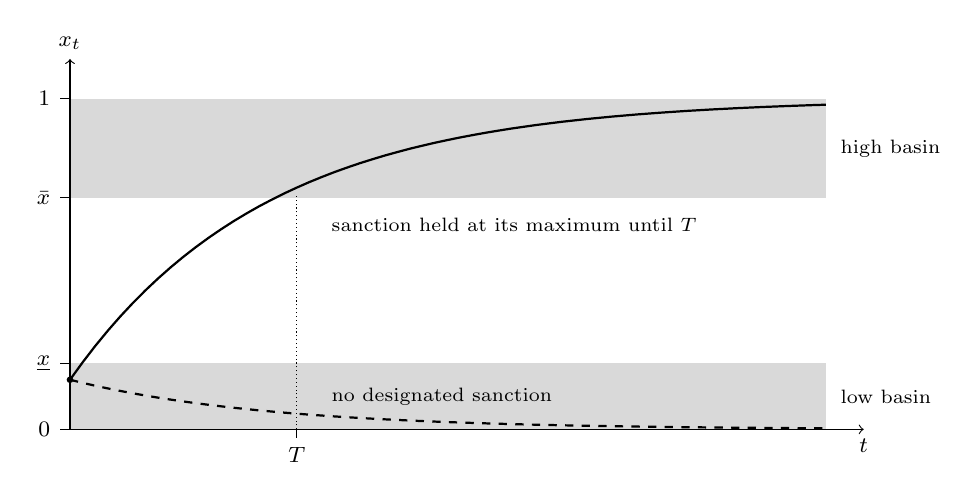
\begin{tikzpicture}[x=0.32cm,y=4.2cm,font=\footnotesize]
\fill[black!15] (0,0.7) rectangle (30,1);
\fill[black!15] (0,0) rectangle (30,0.2);
\draw[->] (0,0) -- (31.5,0) node[below] {$t$};
\draw[->] (0,0) -- (0,1.12) node[above] {$x_t$};
\foreach \y/\l in {0/0,0.2/\underline{x},0.7/\bar x,1/1} \draw (0,\y) -- (-0.4,\y) node[left] {$\l$};
\draw (9,0) -- (9,-0.025) node[below] {$T$};
\draw[densely dotted] (9,0) -- (9,0.71);
\draw[thick,domain=0:30,samples=61] plot (\x,{1-0.85*0.88^\x});
\draw[thick,dashed,domain=0:30,samples=61] plot (\x,{0.15*0.88^\x});
\fill (0,0.15) circle (1.2pt);
\node[anchor=west,font=\scriptsize] at (10,0.62) {sanction held at its maximum until $T$};
\node[anchor=west,font=\scriptsize] at (10,0.1) {no designated sanction};
\node[anchor=west,font=\scriptsize] at (30.2,0.85) {high basin};
\node[anchor=west,font=\scriptsize] at (30.2,0.1) {low basin};
\end{tikzpicture}
\caption{The path of the political state from the same start $x_0$ in the low basin
$[0,\underline x]$, under the partial-adjustment law. Dashed: without a designated
sanction the state stays in the low basin, where realized sanctions do not rise.
Solid: a sanction held at its maximum until date $T$ carries the state into the
high basin $[\bar x,1]$, after which equilibrium play keeps it there and the
sanction never falls (\Cref{prop:lock-in}).}
\label{fig:state-path}
\end{figure}

% @econ-contract paragraph
% id: DISC_BLUFFING
% role: Relate the designated sanction to bluffing under incomplete information (the author, 2026-10-17: "cite other paper's bluffing result ... they actually turn the bluffing to be true, and that caused the persist sanctions under this model"): a sanction imposed as a bluff, or to call one, and held long enough moves the state into the high basin, where continuing it is equilibrium play.
% depends_on: DISC_DESIGNATED_SANCTION
% handoff: Relief in practice.
% exact_ref: bib:Spaniel2015#pp=735-736,739
% source_role: bib:Spaniel2015#pp=735-736,739 => Under uncertainty about leader strength, weaker target leaders have incentives to bluff strength by continuing a crisis, and foreign powers sometimes call potential bluffs by implementing sanctions (read 2026-10-17 from the PDF); the bluffing result the paragraph builds on, not support for a result of this paper.
% exact_ref: bib:Brekhov2022#p=77
% source_role: bib:Brekhov2022#p=77 => Analyses targets' incentives to bluff under sanction (and reward) regimes in a repeated interaction with asymmetric information (read 2026-10-17 from the PDF); positioning only.
% exact_ref: tex-label:prop:lock-in
% support_status: VERIFIED
% status: PROPOSED
% @end-econ-contract
\central{Sanctions that begin as bluffs can become self-sustaining under equilibrium
play.} Under incomplete information, imposing sanctions can serve as a bluff or as a way
to call an opponent's bluff. In \citet[pp.~735--736]{Spaniel2015}, weaker target leaders
have ``incentives to bluff strength'' by continuing a crisis, and foreign powers respond
``by sometimes conceding and sometimes calling potential bluffs by implementing
sanctions''; \citet[p.~77]{Brekhov2022} analyzes target incentives to bluff under
sanctions. In those models, information revealed during the crisis determines subsequent
outcomes. Here, sanctions also shift the political state. A sanction imposed as a
bluff---or to call an opponent's bluff---and maintained for a sufficient duration acts as
a designated sanction in the sense defined above: it moves the state into the high basin,
where continued sanctioning is prescribed by equilibrium play. The bluff then becomes
self-fulfilling, and sanctions persist without any beliefs to revise.

\subsection{Real-world sanctions relief}
\label{sec:discussion:relief}
\label{sec:discussion:evidence}

% @econ-contract paragraph
% id: DISC_THREE_QUESTIONS
% role: Separate preference for relief, belief that it will be honoured, and its usability, and state the participation result (prop:relief-participation) at its scope, in words, as the model's answer to the first question.
% depends_on: DISC_BLUFFING
% handoff: Credibility of relief.
% merged_from: DISC_PARTICIPATION
% exact_ref: tex-label:prop:relief-participation
% support_status: NOT_APPLICABLE
% status: PROPOSED
% @end-econ-contract
\central{A natural application of the model is to proposals for sanctions relief, which raise
three related but distinct questions; the model's incentive comparisons speak to the
first.}\footnote{The participation
result is proved in \Cref{app:proofs:branch} of the Online Appendix; the economy
at which a temporary suspension of sanctions benefits a non-compliant target is recorded in the
formal supplement.}
Would policymakers prefer the arrangement and expect it to be honored, and would nominal
relief restore the economic activity it is intended to enable? On the first question,
consider a temporary suspension of sanctions followed by any equilibrium where the target
maintains full non-compliance, such as the constructed equilibrium. Under the
entrenchment condition and a sender response at full non-compliance that does not
decrease with the state, the change in incumbent payoffs does not support any date-zero
side payment between governments that would make the shock mutually acceptable. That
neither incumbent gains from such a shock follows jointly from three conditions: the
sender's positive marginal return to sanctioning a non-compliant target, the property
that compliance does not increase the sender's payoff at zero sanctions, and the
entrenchment condition. For an economy failing the entrenchment condition, a temporary
suspension of sanctions benefits a target that still does not comply.

% @econ-contract paragraph
% id: DISC_CREDIBILITY
% role: Tie the credibility of relief to commitment technologies and to lock-in, with the relief credibility point.
% depends_on: DISC_THREE_QUESTIONS
% handoff: Rival accounts of non-relief.
% exact_ref: bib:Powell2012#scope=paper
% source_role: bib:Powell2012#scope=paper => Already-cited source that singles out a costlessly reversible concession as least credible; it does not model this paper's state channel.
% support_status: UNVERIFIED
% status: PROPOSED
% @end-econ-contract
\central{The second question---whether relief will be honored---depends on commitment
technologies.} Lock-in depends on the initial state, and within a high basin resumed
equilibrium play generates no endogenous exit under the set and level conditions of
\Cref{prop:lock-in}. Expiry dates, review clauses, and other commitment technologies
operate by altering the strategic environment. Relief poses the hardest test for such
mechanisms. Relief that is reversible at no direct cost is the type that
\citet[p.~627]{Powell2012} identifies as least credible. In recent bargaining models of
war, the reliability of an agreement remains a parameter \citep{Ruggiero2026}. A full
model of relief institutions would need to specify, as separate primitives, who can
commit, who holds veto power, how private actors respond, and how these choices alter the
continuation game.

% @econ-contract paragraph
% id: DISC_RIVAL_ACCOUNTS
% role: Place rival accounts of non-relief without dismissing them as non-optimising (repair C6).
% depends_on: DISC_CREDIBILITY
% handoff: What the case material supports.
% exact_ref: bib:HalcoussisKaempferLowenberg2021#scope=paper
% source_role: bib:HalcoussisKaempferLowenberg2021#scope=paper => Already-cited legislative-cost account of sanction persistence; cited as an alternative, not as support for this model.
% support_status: UNVERIFIED
% status: PROPOSED
% @end-econ-contract
\central{Commitment problems are one explanation for persistent non-relief among
several; the model isolates a distinct mechanism.} In this mechanism, continued sanctions
can be optimal because of the state that sanctions have built, provided that the sender
values that target-side state and the entrenchment condition holds. Sanctions can be
optimal even if they are re-optimized every period and a lower sanction level is
feasible. Legislative constraints \citep{HalcoussisKaempferLowenberg2021}, administrative
persistence, and reputational incentives offer alternative explanations. Political or
reputational costs can themselves be incorporated into an optimizing decision
framework.

% @econ-contract paragraph
% id: DISC_PREDICTIONS
% role: State the two observable responses the classification separates, as model implications, not validation.
% depends_on: DISC_RIVAL_ACCOUNTS
% handoff: The case material.
% exact_ref: tex-label:thm:four-cells
% support_status: VERIFIED
% status: PROPOSED
% @end-econ-contract
\central{Comparisons across constructed equilibria distinguish two observable responses
to a single sanctions regime: greater compliance and deeper entrenchment.}\footnote{The
model's predictions are collected in \Cref{app:moved-ah} of the Online Appendix,
and the case sources' discussion of evasion and enforcement in
\Cref{app:moved-ad}.} Greater
compliance arises when the target's forward-looking incentive is weak and a
forward-looking sender raises the cost of relief; deeper entrenchment arises when that
incentive is strong and a forward-looking sender raises the steady-state level.

% @econ-contract paragraph
% id: DISC_CASE_MATERIAL
% role: Use the already-cited case material as motivation for the mechanism, with the Sender's stake kept as a maintained restriction.
% depends_on: DISC_PREDICTIONS
% handoff: The relief cases.
% exact_ref: bib:HaggardNoland2017#scope=paper
% source_role: bib:HaggardNoland2017#scope=paper => Already-cited account of an authoritarian target passing sanction costs to citizens; motivates the mechanism, does not identify any parameter.
% exact_ref: bib:UNPanelDPRK2024#scope=paper
% source_role: bib:UNPanelDPRK2024#scope=paper => Already-cited report of tighter control under sanctions; motivation only.
% support_status: UNVERIFIED
% status: PROPOSED
% @end-econ-contract
\central{North Korea, a context in which this feedback mechanism may be salient, helps
motivate the analysis.} \citet{HaggardNoland2017} describe an authoritarian target able
to pass sanction costs onto its citizens and a leadership reluctant to weaken its control
over foreign economic activity; in the model's terms, these correspond to low sanction
pain and a high valuation of the state---the two sides of the entrenchment condition. A
United Nations Panel of Experts report documents tighter economic, social, and political
controls and more centralized economic management under sanctions
\citep{UNPanelDPRK2024}. These same sources document evasion, enforcement, and
coordination challenges, which can coexist with the political-state feedback
mechanism.

% @econ-contract paragraph
% id: DISC_CASE_RELIEF
% role: Use the Iranian and Russian relief material (note N134, promoted 2026-10-02) to separate acceptability, credibility and delivery of relief, as motivation only.
% depends_on: DISC_CASE_MATERIAL
% handoff: The limits of the equilibrium interpretation.
% exact_ref: tex-label:sec:discussion:relief
% exact_ref: bib:BajoghliNasrSalehiIsfahaniVaez2024#pp=115-116,121-123
% source_role: bib:BajoghliNasrSalehiIsfahaniVaez2024#pp=115-116,121-123 => The authors' account (read 2026-10-02) that the prospect of lifting brought Iran to the 2015 agreement while rollback was slow, could be blocked or reimposed through Congress, and was made immaterial by remaining financial sanctions; motivation for separating the three relief questions, not a test of the model.
% exact_ref: bib:SnegovayaFentonDolbaiaBergmann2025#pp=26,31-32
% source_role: bib:SnegovayaFentonDolbaiaBergmann2025#pp=26,31-32 => The report's description (read 2026-10-02) of Russian businesses that thrive under isolation and fear returning competition, against firms that would gain from partial relief, with its scenario assumptions; heterogeneous interests, projections rather than observed outcomes.
% support_status: UNVERIFIED
% status: PROPOSED
% @end-econ-contract
\central{Iran and Russia illustrate all three questions raised above.} According to
\citet[pp.~115--116]{BajoghliNasrSalehiIsfahaniVaez2024}, the prospect of earlier
sanctions being lifted---not the threat of additional sanctions---brought Iran to the 2015
agreement. Yet the rollback was gradual and required political support at multiple levels
of the United States government. Congress, which is often involved in delisting
decisions, could impose additional hurdles or reimpose the same sanctions under another
pretext, and sanctions remaining on Iran's financial and banking system made the lifting
of others immaterial (pp.~121--123). Accepting relief, expecting it to be honored, and
being able to benefit from it are therefore distinct margins. In Russia, businesses that
have thrived under reduced competition fear the return of Western competitors, while
import- and export-dependent firms could gain from partial sanctions relief
\citep[pp.~31--32]{SnegovayaFentonDolbaiaBergmann2025}. The report's scenarios are
projections from 2025 (p.~26). This heterogeneity is what the political state variable
summarizes.

\subsection{Scope and limitations}
\label{sec:discussion:scope}

% @econ-contract paragraph
% id: DISC_SCOPE
% role: State the mechanism the model isolates and the object of its theorems for a specified instrument and compliance demand; effectiveness judged against a sender's objectives; how the class specializes to other coercive systems.
% depends_on: DISC_CASE_RELIEF
% handoff: The equilibrium concept and the results that reach beyond the constructed equilibria (repair C2).
% exact_ref: bib:GAO2025RussiaSanctions#pp=14
% source_role: bib:GAO2025RussiaSanctions#pp=14 => The report's three categories of objectives (read 2026-10-02); names the objectives against which effectiveness is judged, supports no model result.
% support_status: NOT_APPLICABLE
% status: PROPOSED
% @end-econ-contract
\central{We have deliberately isolated one public-choice mechanism behind persistent sanctions:
sanctions strengthen the target-side constituency that supports their continuation, and
both governments value that constituency.} Within the class, compliance affects the
sender by reducing its incentive to sanction. Given a coercive instrument and a
compliance demand, the theorems characterize how equilibrium play evolves from the
political state that sanctions---once imposed---have altered. Effectiveness, by contrast,
is measured against a sender's objectives, which the U.S. Government Accountability
Office identifies for U.S. measures on Russia as economic pressure, inhibition of the war
effort, and accountability \citep[p.~14]{GAO2025RussiaSanctions}. The mathematical
structure of the class can be adapted to other coercive systems. Doing so requires
mapping their actions, constituency effects, and payoff signs into the class structure,
including analogues of each government's stake in the state and of the entrenchment
condition.

% @econ-contract paragraph
% id: MODEL_EQUILIBRIUM_SCOPE
% role: How existence is obtained (by construction on invariant sets of value functions), and the concept against strong stationary Stackelberg and history-dependent equilibria (moved from Section 2.4, 2026-10-16, structure plan S4).
% depends_on: DISC_SCOPE
% handoff: The objects solved jointly and the results beyond the constructed equilibria.
% exact_ref: tex-label:thm:existence
% exact_ref: bib:HeLiuChen2025#scope=paper
% source_role: bib:HeLiuChen2025#scope=paper => Already-cited dynamic feedback Stackelberg existence and computation antecedent (restored 2026-10-02 after the rebuild dropped it); positions the joint-iteration existence route, does not prove it.
% exact_ref: bib:LiSojoudiTomlinFridovichKeil2024#scope=paper
% source_role: bib:LiSojoudiTomlinFridovichKeil2024#scope=paper => Already-cited feedback Stackelberg computation antecedent (restored 2026-10-02 after the rebuild dropped it); positioning only.
% exact_ref: tex-label:prop:history-deviations
% support_status: VERIFIED
% status: PROPOSED
% @end-econ-contract
\central{Existence is established by construction, and each construction pins down its
equilibrium only within the sets of value functions it employs.} Where the results
construct a value function, it is the unique fixed point of its Bellman operator defined
over an explicitly stated \emph{invariant set of value functions}: a closed set with
stated bounds on the level and slope of each member (and on
curvature for the sender), which the operator maps into itself. \Cref{sec:results} constructs
equilibria over the full class of economies. A general existence argument---based on
joint contraction of both Bellman equations when the coupling between them is
sufficiently weak---follows in the spirit of \citet{StokeyLucas1989} and of broader
research on the existence and computation of dynamic feedback Stackelberg equilibria
\citep{HeLiuChen2025,LiSojoudiTomlinFridovichKeil2024}.

\central{Two comparisons delineate the scope of the equilibrium concept: with the
stationary strong Stackelberg equilibrium, and with history-dependent strategies.}
First, target optimality in $\mathcal E$ is pointwise: at each state, the target
maximizes the right-hand side of \eqref{eq:T-bellman}, taking continuation values as
given. In a stationary strong Stackelberg equilibrium, by contrast, the leader selects an
entire policy function and anticipates that the follower re-optimizes after every policy
deviation; the two concepts need not coincide \citep{Bucarey2023,KudoAkimoto2026}. The
equilibrium concept is time-consistent because both governments re-optimize at every
state. Second, against any equilibrium in $\mathcal E$, no pure strategy conditioned on
the entire history outperforms the equilibrium's own play, from any initial state
and---for the sender---after any observed compliance level on or off the equilibrium
path.

% @econ-contract paragraph
% id: DISC_EQUILIBRIUM_LIMITS
% role: State the equilibrium notion, the objects it solves jointly, and the two results that reach beyond the constructed equilibria (repair C2).
% depends_on: MODEL_EQUILIBRIUM_SCOPE
% handoff: Levels of generality.
% merged_from: DISC_ENDOGENOUS
% exact_ref: tex-label:prop:security
% note: 2026-10-16 (structure plan S4): the Markov sentence is in Section 2.4 and the minmax and uniqueness results in Section 3.4; this paragraph points there.
% support_status: VERIFIED
% status: PROPOSED
% @end-econ-contract
\central{Within each equilibrium, the target's compliance rule, the sender's sanction
rule, both value functions, both feedback policies, and the political-state trajectory
are solved jointly.} In the interest-group polity, the pressure levels of competing
groups also constitute a Nash equilibrium of the political contest. Two results extend
beyond the constructed equilibria under the strong entrenchment condition: the target's
minmax payoff bound and the uniqueness of full non-compliance among non-decreasing
sanction rules (\Cref{sec:results:security}).

% @econ-contract paragraph
% id: DISC_GENERALITY_LEVELS
% role: Separate results about every equilibrium satisfying stated conditions, results derived from primitives on the class, and results established at example economies, citing main-text results only.
% depends_on: DISC_EQUILIBRIUM_LIMITS
% handoff: Open extensions.
% exact_ref: tex-label:prop:certified-equilibria
% support_status: VERIFIED
% status: PROPOSED
% @end-econ-contract
\central{The results operate at three levels of generality.} First, some apply to every
equilibrium satisfying stated conditions: lock-in (\Cref{prop:lock-in}) applies to every
equilibrium meeting its basin conditions and, for entry, its transition conditions; the
fixed-target-policy comparison (\Cref{thm:dominance}) applies to every non-decreasing
sender value at every state, and thus to every equilibrium containing one; the premium bound
of \Cref{sec:results:wedge} applies to every equilibrium with a non-increasing target
policy, for economies in the class with an upper bound on the substitution rate at which
larger concessions are never worth more to the sender at zero sanctions; and the minmax
bound applies to every equilibrium in $\mathcal E$. Second, the myopic-benchmark
comparison (\Cref{thm:regime-separation}), the four-case characterization
(\Cref{thm:four-cells}), and the threshold result (\Cref{prop:collapse-threshold}) derive
equilibrium properties and dynamics from inequalities across primitives over the class, and
greater target patience preserves the full-non-compliance equilibrium that exists at a
lower discount factor (\Cref{prop:patience-existence}). The welfare results of
\Cref{sec:welfare} hold across the class, as do the rescaling property and the planner
optimality condition for any representation and any bounded welfare flow. Third, some
results are established via example economies, which demonstrate that hypotheses can be
satisfied or bounds attained: the welfare loss in one interest-group polity
(\Cref{sec:welfare:efficiency}), the attainment of the premium bound
(\Cref{sec:results:wedge}), and economies satisfying the lock-in conditions
(\Cref{app:persistence:reading} of the Online Appendix).

% @econ-contract paragraph
% id: DISC_OPEN
% role: Name the extensions and the measurement requirements for empirical work.
% depends_on: DISC_GENERALITY_LEVELS
% handoff: The conclusion.
% exact_ref: bib:AttiaGrauvogel2023#scope=paper
% source_role: bib:AttiaGrauvogel2023#scope=paper => Already-cited exploratory association between institutional clauses and termination; not a causal estimate and not support for a model result.
% support_status: UNVERIFIED
% status: PROPOSED
% @end-econ-contract
\central{Two broad kinds of extensions build on these results: empirical measurement of
the political state and its associated payoff terms, and richer theoretical models of
the state and of relief institutions.} Disciplining estimates of the political-state
transition and the payoff terms governing basin entry would require empirical measures
that separate the political state from aggregate income, and distinguish within-target
adjustment from selection across surviving episodes. Theoretical extensions could
incorporate multidimensional political states, stochastic shock duration,
forward-looking investment by groups in their own future power
\citep{AcemogluRobinson2008}, or explicit relief and commitment technologies. The last of
these could alter entry into or create exit from the high basin, and
\citet{AttiaGrauvogel2023} document exploratory empirical associations between such
provisions and sanction termination. A fully optimal relief policy would require explicit
institutional instruments and commitment constraints. A symmetric framework in which both
governments directly move the state---of the kind \citet{Powell2013} calls for---would
embed compliance directly into the transition law and require rederiving the argument
that compliance reduces the sender's incentive to sanction.

% @econ-contract include
% id: INCLUDE_CONCLUSION
% file: main_sections/06_conclusion.tex
% section_contract: CONCLUSION_ANSWER
% role: Answer the question at its proved scope and state its limits.
% question_answered: What was established, and where does it stop?
% required_inputs: All result sections.
% output_handoff: None.
% claim_ceiling: The master plan's ceiling; no policy prescription.
% status: HUMAN_CONFIRMED
% @end-econ-contract
% @econ-contract section
% id: CONCLUSION_ANSWER
% role: Answer the question at its proved scope: the mechanism and answer first; who decides accommodation, who decides intensity; what the reach results add; the persistence and welfare limits.
% question_answered: What did the paper establish, and where does it stop?
% required_inputs: RESULTS_HORIZONS, WELFARE_BOUNDARY, DISCUSSION_INTERPRETATION.
% output_handoff: None.
% claim_ceiling: The master plan's ceiling; no policy prescription.
% exclusions: A theorem list; new claims.
% exact_ref: tex-label:sec:conclusion
% support_status: VERIFIED
% status: HUMAN_CONFIRMED
% human_confirmed_at: 2026-10-01
% decision_ref: suggestions/2026-10-01-manuscript-rebuild/01_STRUCTURE_PROPOSAL.md#author-decisions-recorded
% confirmation_scope: Section role and claim ceiling.
% reopen_if: A principal result or the claim ceiling changes.
% amended_at: 2026-10-12 (opens on the dual-basin illustration and states its limits; decision_ref: suggestions/2026-10-10-jet-submission/DECISIONS.md#framing-2026-10-12); 2026-10-13 (argument plan: mechanism and answer first, then the dual-basin illustration with its limits, the reach results, welfare and lock-in, and a closing 'so what / now what' paragraph; decision_ref: suggestions/2026-10-10-jet-submission/exposition-2026-10-13/ARGUMENT_PLAN.md); 2026-10-15 (the dual-basin illustration dropped from the main text for now, on the author's word); 2026-10-19 (coauthor wording review: wording of the coauthor's line-by-line revision applied where not wrong; sender/target in lower case; non-compliance for defiance; decision_ref: suggestions/2026-10-10-jet-submission/DECISIONS.md#coauthor-wording-review-2026-10-19); 2026-10-20 (humanizer pass: dashes replaced by commas, parentheses or colons; plain wording; meaning unchanged; decision_ref: suggestions/2026-10-10-jet-submission/DECISIONS.md#humanizer-pass-2026-10-20)
% @end-econ-contract
\section{Conclusion}
\label{sec:conclusion}

% @econ-contract paragraph
% id: CONCLUSION_ROLES
% role: Open with the mechanism and the answer on the class (the myopic benchmark ends sanctions, forward-looking governments sustain them; the Target's patience decides relief against defiance), then the Sender's role and the same-policy comparison with its hypothesis (repair C4). Moved first (argument plan, 2026-10-13); reordered on the layout decisions of 2026-10-16.
% depends_on: CONCLUSION_ANSWER
% handoff: The reach results.
% exact_ref: tex-label:prop:myopic-benchmark
% exact_ref: tex-label:thm:regime-separation
% exact_ref: tex-label:thm:four-cells
% exact_ref: tex-label:thm:dominance
% support_status: VERIFIED
% status: PROPOSED
% @end-econ-contract
\central{Economic sanctions can persist because they strengthen the domestic political
interests that support their continuation.} Without foresight they unravel: in the
myopic benchmark, the target accommodates and the political state erodes over time. In
the equilibria constructed over the class of economies, when both governments value the
political state and are forward-looking, the target maintains non-compliance, sanctions
persist indefinitely, and the political state converges to a positive steady-state
level. The target's patience determines whether relief or non-compliance prevails;
whether the sender is forward-looking shapes the compliance threshold for relief or the
intensity of sanctions under non-compliance. These comparisons hold all non-discount
primitives fixed. For a fixed target policy, a non-decreasing sender continuation value
weakly increases the largest of the optimal sanctions relative to the myopic best response. Under
interiority, the constructed equilibria exhibit a strictly positive foresight premium
relative to the myopic best response, with a closed-form lower bound.

% @econ-contract paragraph
% id: CONCLUSION_REACH
% role: Summarize the reach results: patience, like the Target's other parameters, can change whether full defiance is an equilibrium; result names in place of condition lists (argument plan, 2026-10-13).
% depends_on: CONCLUSION_ROLES
% handoff: The welfare findings and lock-in.
% exact_ref: tex-label:prop:security
% exact_ref: tex-label:prop:collapse-threshold
% support_status: VERIFIED
% status: PROPOSED
% @end-econ-contract
\central{Beyond the constructed equilibria, patience, like all other target
parameters, shapes whether full non-compliance is supportable as an equilibrium.} When
the sender's response and the target's value under full non-compliance do not decrease
with the state, greater target patience preserves the full-non-compliance equilibrium.
Under the strong entrenchment condition, the target guarantees itself a minmax payoff
against every pure sanction strategy, bounding its payoff in every equilibrium from
below; and across the class, every equilibrium with a non-decreasing sanction rule
exhibits full non-compliance. In the special case of \Cref{prop:collapse-threshold}, a
full-non-compliance equilibrium exists if and only if the target's discount factor is at
least a threshold value.

% @econ-contract paragraph
% id: CONCLUSION_LIMITS
% role: State the welfare findings, then lock-in and persistence without hysteresis, naming prop:lock-in instead of listing its conditions (argument plan, 2026-10-13).
% depends_on: CONCLUSION_REACH
% handoff: So what and now what.
% exact_ref: tex-label:sec:welfare
% exact_ref: tex-label:prop:lock-in
% support_status: VERIFIED
% status: PROPOSED
% @end-econ-contract
\central{Persistent sanctions can be socially costly, and the game alone does not
determine their welfare ranking.} Across the class, two interest-group representations
of the same government payoffs rank the constructed equilibria in opposite orders, and
under compliance neutrality one makes persistent play socially optimal. For an example
economy with one explicit interest-group polity, equilibrium sanctions remain at their
maximum level and generate welfare losses.

The political state can also lock in sanctions. Where an equilibrium and a high-state
interval satisfy the conditions of \Cref{prop:lock-in}, a state entering the interval
remains there under equilibrium play and sanctions never decline. When full sanctions
raise every state below the basin, a sufficiently long temporary shock can produce a
durable outcome. Persistence can also arise without hysteresis. Where the explicit
Lipschitz constant derived for the constructed equilibrium's law of motion is strictly
below one, a temporary shock has no permanent asymptotic effect.

% @econ-contract paragraph
% id: CONCLUSION_SO_WHAT
% role: Say what the results mean (persistence need not reveal failed bargaining or misperception; with information complete, the levers act on the political state and the governments' incentives, not on beliefs) and what would discipline the channel (measurement, sec:discussion:scope), with no prescription; close on the paper's answer.
% depends_on: CONCLUSION_LIMITS
% handoff: None.
% origin: argument plan item 10 (2026-10-13); the closing sentence moved here from CONCLUSION_LIMITS.
% exact_ref: tex-label:sec:discussion:scope
% exact_ref: tex-label:sec:discussion:misperception
% support_status: VERIFIED
% status: PROPOSED
% @end-econ-contract
\central{Persistent sanctions therefore need not reflect failed bargaining or
misperception.} Within the model, they can be the optimal choice of governments that
value the political state that sanctions themselves have built. With complete
information, the levers that end sanctions operate through the political state and
government incentives, not through beliefs (\Cref{sec:discussion:misperception} of the
Online Appendix). Whether this channel operates in a given episode is an empirical
question: measurements that separate the political state from aggregate income would
discipline estimates of its transition and of the payoff terms governing basin entry
(\Cref{sec:discussion:scope}). \central{Optimizing governments can thus perpetuate and
lock in sanctions through the political state that sanctions generate; patience and
other economic features determine whether this occurs.}

% @econ-contract include
% id: INCLUDE_DECLARATIONS
% file: main_sections/07_declarations.tex
% section_contract: DECLARATIONS_STATEMENTS
% role: Carry the required author declarations.
% question_answered: Competing interests, funding, contributions, AI use, data availability.
% required_inputs: Author records.
% output_handoff: None.
% claim_ceiling: Declarations only; no scientific claim.
% status: HUMAN_CONFIRMED
% @end-econ-contract
% @econ-contract section
% id: DECLARATIONS_STATEMENTS
% role: Carry the required author declarations.
% question_answered: Competing interests, funding, contributions, AI use, data availability.
% required_inputs: Author records.
% output_handoff: None.
% claim_ceiling: Declarations only; no scientific claim.
% exclusions: Any scientific claim.
% support_status: NOT_APPLICABLE
% status: HUMAN_CONFIRMED
% human_confirmed_at: 2026-10-01
% decision_ref: suggestions/2026-10-01-manuscript-rebuild/01_STRUCTURE_PROPOSAL.md#author-decisions-recorded
% confirmation_scope: Section role only; the declarations' content is the author's.
% reopen_if: Journal requirements or the author's declarations change.
% amended_at: 2026-10-19 (data availability names the release v1.30-submission; decision_ref: suggestions/2026-10-10-jet-submission/DECISIONS.md#submission-release-2026-10-19); 2026-10-20 (the repository link; decision_ref: suggestions/2026-10-10-jet-submission/DECISIONS.md#repository-link-and-acemoglu-notes-2026-10-20); 2026-10-20 (the release is public at the new repository; decision_ref: suggestions/2026-10-10-jet-submission/DECISIONS.md#public-repository-2026-10-20); 2026-10-21 (Elsevier layout: the generative-AI statement is its own section, titled as the Guide requires, last before the references, wording otherwise unchanged; funding in the Guide's sentence; data availability without the internal script name, citing the release; decision_ref: suggestions/2026-10-10-jet-submission/DECISIONS.md#jet-submission-package-2026-10-21)
% @end-econ-contract
\section*{Declarations}

% Coauthors' confirmation of no competing interests: received (the author, 2026-10-21).
\paragraph{Declaration of competing interest.} The authors declare no
competing financial interests or personal relationships that could have
influenced the work reported in this paper.

\paragraph{Funding.} This research did not receive any specific grant from funding
agencies in the public, commercial, or not-for-profit sectors.

\paragraph{CRediT author statement.} Xiaofeng Gong:
Conceptualization, Formal analysis, Methodology, Software, Validation,
Visualization, Writing -- original draft, and Writing -- review and
editing. Yuechuan Zhao: Conceptualization, and Writing -- review and
editing. Chunping Zhong: Conceptualization, and Writing -- review and
editing.

\paragraph{Data availability.} No empirical data were used. The Lean~4 formalization
that machine-checks the core results of this paper, as mapped in the formal supplement, is
public as the release \texttt{v1.30-submission} at
\url{https://github.com/qidaolake/political-entrenchment-sanctions-lean}
\citep{GongLean2026}, with the manuscript, the Online Appendix and the formal supplement
attached to it. Its source archive accompanies this submission as supplementary material.
A deposit with a DOI will accompany publication.

\paragraph{Formalization methods.} The Lean~4 development was written with
assistant-generated suggestions for proof steps and lemma search. The
selection of the statements to formalize, the economic interpretation of
every formal statement, and the correspondence map between the manuscript
and the declarations were made and reviewed by the authors, and the Lean~4
kernel independently checks every proof term in the archived release. A
kernel check certifies a formal statement; it does not certify that an
informal economic sentence translates that statement faithfully, which is
why the correspondence is recorded as a separately reviewed map in the
formal supplement.


% ---------------------------------------------------------------------
% COMBINED mode only: inline the appendix so that a single PDF carries
% both the manuscript and the appendix under one bibliography.
% ---------------------------------------------------------------------


\ifdefined\COMBINEDAPPENDIX
% @econ-contract include
% id: INCLUDE_APPENDIX_BODY
% file: sanctions_appendix_body.tex
% section_contract: APPENDIX_INDEX
% role: Inline the appendix in the combined build only; the split build cross-references the standalone appendix.
% question_answered: Where are the exact statements, proofs, constructed economies and the formalization map?
% required_inputs: All main sections.
% output_handoff: None.
% claim_ceiling: Exact statements and proofs of the results the main text states; no further claim.
% status: HUMAN_CONFIRMED
% @end-econ-contract
  % @econ-contract section
% id: APPENDIX_INDEX
% role: Order the appendix in three parts: general results for abstract payoffs and transitions in the class (conditions and component statements, proofs, persistence and lock-in, existence, discharge routes, supporting results, further statements); examples (parametric families and the roster, numerical economies, closed-form constants, the interest-group example); the literature (the author's decision, 2026-10-20); within each part, what the main text needs comes before derivative and supplementary material (2026-10-20).
% question_answered: Where is each exact statement and proof?
% required_inputs: The main sections.
% output_handoff: None.
% claim_ceiling: Exact statements and proofs of results the main text states; machine-checked statements as recorded in the formalization map.
% exclusions: New claims not stated or summarised in the main text.
% exact_ref: file:appendix_sections/07_formalization_map.tex#label=app:formalization
% source_role: file:appendix_sections/07_formalization_map.tex#label=app:formalization => The formal supplement's formalization map, which records the Lean declaration behind each statement; it establishes formal derivation, not economic correspondence.
% support_status: VERIFIED
% status: HUMAN_CONFIRMED
% human_confirmed_at: 2026-10-01
% decision_ref: suggestions/2026-10-01-manuscript-rebuild/01_STRUCTURE_PROPOSAL.md#author-decisions-recorded
% confirmation_scope: Appendix role and the D1 moves.
% amended_at: 2026-10-20 (three parts, general results and examples separated, on the author's "see whether we can have a generalized form abstract functional form appendix versus a numerical example appendix please, make it more organized"; decision_ref: suggestions/2026-10-10-jet-submission/DECISIONS.md#appendix-in-three-parts-and-the-one-sided-cases-paragraph-2026-10-20); 2026-10-20 (within each part, what the main text needs before derivative material; decision_ref: suggestions/2026-10-10-jet-submission/DECISIONS.md#appendix-needed-versus-derivative-2026-10-20); 2026-10-20 (proof maps open Part I; decision_ref: suggestions/2026-10-10-jet-submission/DECISIONS.md#proof-maps-and-reading-the-lean-statements-2026-10-20)
% reopen_if: A section moves between the main text and the appendix.
% @end-econ-contract
% =====================================================================
%  SHARED APPENDIX INDEX  --  sanctions_appendix_body.tex
%
%  This file is NOT a document.  It is \input by BOTH:
%     sanctions_jet_appendix.tex   -> standalone appendix PDF
%     sanctions_jet_draft.tex      -> only in COMBINED mode
%  so the two builds cannot diverge.  It begins at \appendix, inputs the
%  ordered files under appendix_sections/, and ends before the bibliography,
%  which each root supplies for itself.
% =====================================================================

\appendix

% Everything below is an appendix, so cleveref must call it one.  Without
% these two lines \Cref{app:closedforms} typesets as "Section C" -- which,
% now that the appendix is a separate document, names a section the
% manuscript does not contain.  (The \crefnames are in sanctions_preamble.tex.)
\crefalias{section}{appendix}
\crefalias{subsection}{subappendix}
\crefalias{subsubsection}{subappendix}

% Ordered appendix-section index; section bodies live in appendix_sections/.
\section*{How to read this appendix}

\paragraph{Where the main text's proofs are.} Each subsection of the main text
opens with a footnote that points here; the map collects those pointers.
\begin{itemize}
\item Section~\ref{sec:model} (the model): the bounds of the class and the precise conditions
in panel~A0 of \Cref{app:proofs:placable} and in
\Cref{sec:moved-main-2026-10-13:conditions}; the closed-form constants in
\Cref{app:closedforms}; the parametric examples in \Cref{sec:model:examples}; the
example economies in \Cref{app:witness,app:fourgroup}, and the numerical ones, among them the dual-basin
economy, in \Cref{sec:moved-main-2026-10-15,app:dual-basin-economy}; existence in \Cref{app:existencemachinery}.
\item Section~\ref{sec:model:myopic} (the myopic benchmark) and Section~\ref{sec:results:main} (foresight against it):
panel~F of \Cref{app:proofs:placable}; the component statements in
\Cref{sec:moved-main-2026-10-13:components}.
\item Section~\ref{sec:results:wedge} (the target's and the sender's parts): \Cref{app:proofs:branch} and
\Cref{app:proof-dominance}; the strict comparison in
\Cref{sec:moved-main-2026-10-13:strict}.
\item Section~\ref{sec:results:lockin} (lock-in): \Cref{app:persistence}; the low basin in
\Cref{thm:lowbasin}; an equilibrium with both basins in \Cref{app:dual-basin-economy}.
\item Section~\ref{sec:results:patience} (patience): \Cref{app:proofs:threshold,app:proofs:scope}, and
the general conditions in \Cref{sec:moved-main-2026-10-13:bracket}.
\item The end of Section~\ref{sec:results:patience} (minmax and uniqueness): the statements in
\Cref{sec:moved-main-2026-10-13:security}, proved in \Cref{app:proofs:scope}.
\item Section~\ref{sec:welfare} (welfare): the proofs in \Cref{app:proofs:welfare};
\Cref{app:fourgroup} and \Cref{sec:moved-main-2026-10-13:welfare} for the
interest-group polity and the family's microfoundations.
\item Section~\ref{sec:discussion:horizons} (one government forward-looking): the component statements in
\Cref{sec:moved-main-2026-10-13:components}, proved in \Cref{app:proofs:placable};
the welfare reversal across the four cases in \Cref{app:proofs:welfare}.
\item Section~\ref{sec:discussion} (discussion): \Cref{app:persistence,app:decomposition-path}.
\end{itemize}


\paragraph{How the appendix is organized.} The appendix has three parts, and each of
the two larger parts puts what the main text needs before derivative material.
Part~I holds the general results, which hold for abstract payoffs and transitions in the
class, with no functional form. What the main text needs comes first: maps of how the
results are proved (\Cref{app:proof-maps}); the conditions in
full and the component statements of the main results
(\Cref{sec:moved-main-2026-10-13}); the proofs (\Cref{app:proofs}), among them the
construction on the class under the lifting condition with its class-membership panel
(\Cref{app:proofs:placable}); persistence, temporary shocks and lock-in, with the low
basin, relief and the exit duration (\Cref{app:persistence}); and the two-channel
decomposition and the path of the state (\Cref{app:decomposition-path}). The derivative
and supplementary results follow: the existence machinery (\Cref{app:existencemachinery}),
the assumption-discharge routes (\Cref{app:dischargers}), the robustness and boundary
results (\Cref{app:supporting-results}) and further results on persistence and the long
run (\Cref{app:moved-ak}). Part~II holds the examples: the ones the main text uses, the
parametric families with the benchmark economy (\Cref{app:witness}), the numerical
example economies (\Cref{app:numerical-examples}) and the microfounded interest-group
example (\Cref{app:fourgroup}); then further example economies
(\Cref{app:further-examples}) and the closed-form constants of the parametric family
(\Cref{app:closedforms}). Part~III places the paper in the literature
(\Cref{app:literature}). The formalization map, which lists for every statement the
machine-checked declaration that proves it, is in the formal verification supplement.
Every cross-reference in the manuscript resolves into this document.

\section*{Notation and symbols}

This list collects the symbols used repeatedly in the manuscript and
appendix. Symbols confined to a single proof, proposition, or certificate
table are defined locally where they first appear.

\begin{longtable}{@{}p{0.25\textwidth}p{0.69\textwidth}@{}}
\toprule
Symbol & Meaning\\
\midrule
\endfirsthead
\toprule
Symbol & Meaning\\
\midrule
\endhead
$t;\ x_t,\ a_t,\ s_t$
& Date $t\in\mathbb N$; political state, target compliance, and sender
sanction at date $t$, each of the three taking values in $[0,1]$.\\
$\F(x,s)$
& General state-transition law. Conditions \textup{(F1)--(F5)} impose
continuity, monotonicity, diagonal fixed points, and strict adjustment
toward the current sanction.\\
$\delta$
& Adjustment rate in the partial-adjustment law
$\F(x,s)=(1-\delta)x+\delta s$.\\
$\beta_T,\beta_S$
& target and sender discount factors.\\
$\Ut,\Us$
& target and sender one-period government objectives.\\
$\Vt,\Vs$
& target and sender continuation-value functions.\\
$T_T,T_S$
& target and sender Bellman operators.\\
$\gamma_F$
& Optional inherited-state Lipschitz modulus of $\F$ at a fixed sanction.\\
$J_S(x,a,s;\Vs)$
& Dynamic sender objective
$\Us(x,a,s)+\beta_S\Vs(\F(x,s))$.\\
$\sigM$
& The sender's myopic best response.\\
$\sigDyn_{\Vs},\ \sigDynTop_{\Vs}$
& The sender's dynamic argmax and its greatest selection, the dynamic best
response, at continuation value $\Vs$.\\
$\alpha,\ \alphaM$
& Equilibrium target policy and the independently optimized myopic target
policy.\\
$\alpha_{V_T,V_S}$
& target argmax policy induced by a value pair in
$\mathcal C_T\times\mathcal C_S$.\\
$E,\ \mathcal E$
& A stationary feedback Stackelberg equilibrium
$E=(\Vt,\Vs,\alpha)$ and the set of all such equilibria.\\
$M=(\alphaM,\sigM)$
& Myopic equilibrium. This roman $M$ is distinct from the
bold row-Lipschitz matrix $\mathbf M$ below.\\
$(x_t^E,s_t^E),\ (x_t^M,s_t^M)$
& Realized state and sanction paths of the equilibrium and of the myopic
equilibrium from the common initial state $x_0$.\\
$\bar x_T,\bar x_S;\ \bar x;\ \basin$
& target and sender tipping thresholds; their joint pivot
$\bar x=\max\{\bar x_T,\bar x_S\}$; and the high basin
$\basin=[\bar x,1]$.\\
$\bar s$
& Sanction-floor parameter used to construct the flip sets.\\
$\mathcal C_T,\mathcal C_S$
& target and sender value sets.\\
$L_{S,x}^{\alpha},\ K_S$
& Composite sender stage-payoff state modulus and the resulting Lipschitz
constant of the sender's value set. The latter is distinct from the sans-serif
commercial-lobby label $\KSgroup$.\\
$m_S,\ c_\sigma$
& sender stage lower-slope level and strict-concavity modulus.\\
$\mathcal F_T(\bar s),\
  \mathcal F_S(\bar s;m_S)$
& target and sender upper flip sets used to derive the basin thresholds.\\
$x_S^0,\ x_S(a)$
& Static sender flip and the sender's per-action flip threshold.\\
$\mathbf M$
& Joint Bellman row-Lipschitz matrix with entries
$\beta_T,L_{TS},L_{ST},\beta_{S,\mathrm{row}}$.\\
$\rho(\mathbf M)$
& Spectral radius of the row-Lipschitz matrix.\\
$R(x),\ G(x)$
& Sanction rule of the equilibrium and closed-loop state-update map,
$R(x)=\sigDynTop_{\Vs}(x,\alpha(x))$ and $G(x)=\F(x,R(x))$.\\
$00,\,01,\,10,\,11$
& The four cases of one economy, target-first: the first index is $1$
when the target is forward-looking ($\beta_T>0$) and $0$ when it is myopic, the
second the same for the sender; $R^{ij}$, $L^{ij}$ and $a^{ij}$ are the
sanction rule, the limit of the political state and the target policy in case
$ij$ (\Cref{sec:four-regimes}).\\
$w_{\mathrm{lo}}$, $w_{\mathrm{hi}}$, $q$, $\bar Q$, $r_{\mathrm{lo}}$,
$r_{\mathrm{hi}}$, $k_{\mathrm{lo}}$, $k_{\mathrm{hi}}$, $u_{\mathrm{lo}}$,
$u_{\mathrm{hi}}$, $\sigma_x$, $\tau_x$
& The class's sender rates: state slope, sanction curvature, state--sanction
cross rate, substitution rate and marginal return to the first
unit of sanction, each as a lower and an upper bound, and the state
semiconcavity and semiconvexity moduli (panel~A0 of
\Cref{app:proofs:placable}).\\
$\ell_{\mathrm{lo}}$, $\ell_{\mathrm{hi}}$, $p_{\mathrm{lo}}$, $c$,
$v_{\mathrm{lo}}$, $n_{\mathrm{lo}}$, $v_{\mathrm{hi}}$, $n_{\mathrm{hi}}$
& The target's rates: compliance cost, sanction pain, and the state slope
$v+ns$ at sanction $s$, each as a lower and an upper bound (panel~A0).\\
$\underline s$
& The lower bound $\sigM(0,0)$: the myopic sanction at full non-compliance at the lowest
state ($u_0/q$ on the quadratic--linear family when $u_0\le q$, as under
interiority).\\
$(q,u_0,k,r,w,\ell,c,n,v)$
& The quadratic--linear family's nine payoff coefficients: sanction-cost curvature,
baseline marginal return to sanctioning, substitution rate, the sender's
state--sanction cross term, sender state valuation, compliance cost, target
sanction pain, the target's state--sanction cross term and target state
valuation (\Cref{sec:model:family}); the transition's slope bounds and moduli
$g_{\mathrm{lo}},g_{\mathrm{hi}},d_{\mathrm{lo}},d_{\mathrm{hi}},M_x,M_m,M_s,
M_{\mathrm{cx}},M_{\mathrm{mix}},M_{\mathrm{cs}}$ are defined in
\Cref{app:proofs:placable}.\\
$x_F,\ x_L$
& Least basin fixed point of $G$ and the limit selected from the basin's
lower endpoint.\\
$\sigma_{\mathrm{real}}$
& A sanction rule held fixed in a transition-law comparison.\\
$d_{\F},\eta_{\F},\widehat N_{\F}$
& Full-sanction drift, its minimum below the basin, and the resulting
conservative shock-duration bound.\\
$P_3,\ h$
& The labeled parameter point $P_3$ of the mechanism-active example economy (a point,
distinct from the persistence condition P3 of \Cref{thm:persistence}) and the
half-width of the box transition shock used in the purification
construction.\\
$\JSgroup,\KSgroup,\JTgroup,\KTgroup$
& Pro-sanction coalition, sender commercial lobby, target regime bloc,
and target opposition in the interest-group polity. Sans-serif lettering
distinguishes these group labels from value-function constants.\\
$W_g,\theta_g,\ W$
& Welfare of group $g$, its political weight, and aggregate welfare,
obtained by setting political weights to one.\\
$g_J,q_K,b_J,b_K,k_S,d_s$
& Interest-group welfare coefficients: sender sanction benefit and loss,
target state valuations, sender sanctioning-cost curvature, and target
sanction-cost rate.\\
$\beta$ (planner)
& Planner discount factor; it is local to that comparison and is distinct
from the government discount factors $\beta_T,\beta_S$.\\
\bottomrule
\end{longtable}

\clearpage


% A group heading inside a part: what the main text needs, then derivative material.
\providecommand{\appendixgroup}[1]{\par\bigskip\noindent{\large\bfseries #1}\par\nopagebreak\medskip}

% Part I: results that hold for abstract payoffs and transitions in the class.
\part{General results: abstract payoffs and transitions}
\appendixgroup{What the main text needs: the conditions, the construction and the proofs}
\section{How the results are proved: maps of the arguments}
\label{app:proof-maps}

The figures in this section show how the paper's results are built. Each box says in
words what a condition requires, what a step constructs, or what a result states. A solid
arrow means that the box at its tail is used to obtain the box at its head. A dashed arrow
means that two results are compared. A dotted arrow marks a step that the result does not
need. Shaded boxes are conditions, plain boxes are steps, and boxes with a heavy border are
results. Below each figure, three lines say what the result proves, what it uses, and the
route of the proof; the proofs themselves are in the sections the figures cite.

\tikzset{
  pm/cond/.style={draw, rounded corners=2pt, fill=black!7, align=left, inner sep=3pt,
    font=\scriptsize},
  pm/step/.style={draw, align=left, inner sep=3pt, font=\scriptsize},
  pm/res/.style={draw, line width=1.1pt, align=left, inner sep=3pt, font=\scriptsize},
  pm/note/.style={align=left, inner sep=1pt, font=\scriptsize\itshape},
  pm/arr/.style={-{Stealth[length=1.7mm]}, semithick},
  pm/cmp/.style={-{Stealth[length=1.7mm]}, semithick, dashed},
  pm/opt/.style={-{Stealth[length=1.7mm]}, semithick, dotted},
}

\subsection{The overall structure}
\label{app:proof-maps:overall}

\par\medskip\noindent\begin{minipage}{\linewidth}\centering
\begin{tikzpicture}[node distance=2.6mm and 7mm]
% conditions (left column)
\node[pm/cond, text width=3.7cm] (law) at (0,0)
  {\textbf{Law of motion} (F1)--(F5): the state persists, rises with the sanction, is kept by
   a sanction equal to it, and moves toward the sanction. Used throughout.};
\node[pm/cond, text width=3.7cm, below=of law] (myo)
  {\textbf{Myopic conditions} (Assumptions 1--3): in one period the sender never sanctions
   fully and lifts the sanction at full compliance; relief is worth its price.};
\node[pm/cond, text width=3.7cm, below=of myo] (conc)
  {\textbf{Concavity} (Assumption 4): the sender has exactly one optimal sanction.
   Maintained on the class.};
\node[pm/cond, text width=3.7cm, below=of conc] (entr)
  {\textbf{Entrenchment and increasing differences} (Assumptions 5--6): the target values the
   entrenchment a sanction builds at least as much as its pain; a more entrenched adversary
   makes sanctioning more attractive.};
\node[pm/cond, text width=3.7cm, below=of entr] (int)
  {\textbf{Interiority and lifting} (Assumptions 7--8): a forward-looking sender never
   sanctions fully and lifts the sanction at full compliance.};
\node[pm/cond, text width=3.7cm, below=of int] (four)
  {\textbf{Four-case conditions}: compliance neutrality, (T6) and (RL).};
\node[pm/cond, text width=3.7cm, below=of four] (lock)
  {\textbf{Lock-in conditions}: value sets, monotonicity and the level condition on a high
   basin; for entry, (F1)--(F4).};
\node[pm/cond, text width=3.7cm, below=of lock] (rep)
  {\textbf{Interest-group representation}: each government's payoff is a weighted sum of
   its groups' welfare.};
% constructions (middle column)
\node[pm/step, text width=4.1cm, right=of myo] (m1)
  {\textbf{The myopic benchmark}: the least compliance $a^{00}(x)$ ends the myopic
   sanction, and with zero sanctions the state erodes.};
\node[pm/step, text width=4.1cm, right=of conc, yshift=-3mm] (m2)
  {\textbf{The sender against full non-compliance}: its value is the fixed point of a
   contraction; its response is unique and above the myopic sanction.};
\node[pm/step, text width=4.1cm, right=of int, yshift=4mm] (m3)
  {\textbf{The target's reply}: full non-compliance is its unique best reply; with the
   target's value, this is an equilibrium in $\mathcal E$.};
\node[pm/step, text width=4.1cm, right=of lock] (m4)
  {\textbf{The high basin}: on it the sender's response stays at or above the state.};
\node[pm/step, text width=4.1cm, right=of rep] (m5)
  {\textbf{Rescaling}: government payoffs fix only weighted sums of group welfare.};
% results (right column)
\node[pm/res, text width=3.7cm, right=of m1] (r1)
  {\Cref{prop:myopic-benchmark}: without foresight, sanctions end and the state falls to
   zero.};
\node[pm/res, text width=3.7cm, right=of m2] (r2)
  {\Cref{thm:regime-separation}: with foresight, the target does not comply, sanctions
   persist, and the state converges above $\underline s$.};
\node[pm/res, text width=3.7cm, right=of law, xshift=4.1cm+7mm+3mm] (r3)
  {\Cref{thm:dominance}: at a fixed target policy, foresight never lowers the sanction.};
\node[pm/res, text width=3.7cm, right=of m3] (r5)
  {\Cref{prop:collapse-threshold,prop:patience-existence}: patience decides between relief
   and non-compliance (with Assumptions 7--8).};
\node[pm/res, text width=3.7cm, right=of m4] (r4)
  {\Cref{prop:lock-in}: the state never leaves the basin, sanctions never fall, and a long
   temporary shock carries the state there.};
\node[pm/res, text width=3.7cm, right=of four, xshift=4.1cm+7mm+3mm] (r6)
  {\Cref{thm:four-cells}: the four cases (with Assumptions 5--8).};
\node[pm/res, text width=3.7cm, right=of m5] (r7)
  {\Cref{prop:welfare-nonidentification}: the game does not pin down the welfare ranking.};
% arrows
\draw[pm/arr] (myo) -- (m1);
\draw[pm/arr] (m1) -- (r1);
\draw[pm/arr] (conc.east) -- (m2.west);
\draw[pm/arr] (entr.east) -- (m3.west);
\draw[pm/arr] (m2) -- (m3);
\draw[pm/arr] (m3.north east) -- (r2.south west);
\draw[pm/cmp] (r1) -- (r2);
\draw[pm/arr] (m3) -- (r5);
\draw[pm/arr] (law.east) -- (r3.west);
\draw[pm/arr] (lock) -- (m4);
\draw[pm/arr] (m4) -- (r4);
\draw[pm/arr] (four.east) -- (r6.west);
\draw[pm/arr] (m3.south east) -- (r6.north west);
\draw[pm/arr] (rep) -- (m5);
\draw[pm/arr] (m5) -- (r7);
\draw[pm/cmp] (r2.east) to[out=-30, in=30, looseness=0.6] (r7.east);
\end{tikzpicture}
\captionof{figure}{The structure of the argument. Left: the conditions, in words. Middle: what the
proofs construct from them. Right: the paper's results. The law of motion is used by every
construction; its one arrow marks the result that needs nothing else from the class
(\Cref{thm:dominance}). Interiority and lifting are named in the result boxes that use
them. The dashed arrows mark comparisons: \Cref{thm:regime-separation} compares with the benchmark,
and \Cref{prop:welfare-nonidentification} ranks the two equilibria.}
\label{fig:proof-map-overall}
\end{minipage}\par\medskip

\noindent\textit{Reading.} Three conditions matter most. Concavity makes the sender's response
unique, the entrenchment condition makes full non-compliance the target's best reply, and
increasing differences make the sender's response rise with the state. The myopic
conditions give the benchmark. The other conditions each serve particular results.\par

\subsection{The constructed equilibrium, \Cref{prop:myopic-benchmark} and \Cref{thm:regime-separation}}
\label{app:proof-maps:main}

\par\medskip\noindent\begin{minipage}{\linewidth}\centering
\begin{tikzpicture}[node distance=3mm and 6mm]
\node[pm/step, text width=6.2cm] (s1) at (0,0)
  {\textbf{Step 1.} The sender's value against full non-compliance is the fixed point of a
   contraction on a set of value functions. Its best response is unique and continuous.};
\node[pm/step, text width=6.2cm, below=of s1] (s2)
  {\textbf{Step 2.} The response lies strictly above the myopic sanction (the foresight
   premium). Under Assumptions 7--8 it is also below the maximum and zero at full
   compliance.};
\node[pm/step, text width=6.2cm, below=of s2] (s3)
  {\textbf{Step 3.} Full non-compliance is the target's unique best reply: compliance lowers
   the sanction, and the entrenchment that sanction builds is worth more than its pain.};
\node[pm/step, text width=6.2cm, below=of s3] (s4)
  {\textbf{Step 4.} The response rises with the state. The target's value is the fixed point
   of a second contraction. Full non-compliance with the two values is an equilibrium in
   $\mathcal E$.};
\node[pm/res, text width=6.2cm, below=of s4] (eq)
  {\textbf{The constructed equilibrium} (\Cref{prop:placable-family}).};
\node[pm/step, text width=6.2cm, below=of eq] (s6)
  {\textbf{Step 6.} The state builds up toward $\underline s$ and lies strictly above the
   myopic path at every positive date.};
\node[pm/step, text width=6.2cm, below=of s6] (s7)
  {\textbf{Step 7.} The closed loop rises with the state, so the path is monotone and
   converges to $x^{11}_\infty$, where the sanction equals the state; $x^{11}_\infty>\underline s$.};
\node[pm/res, text width=6.2cm, below=of s7] (t3)
  {\Cref{thm:regime-separation}: (i) non-compliance and a sanction above the myopic one;
   (ii) build-up and the gap above the benchmark; (iii) convergence above $\underline s$.};
% inputs (left)
\node[pm/cond, text width=3.3cm, left=of s1] (a4) {Concavity (Assumption 4); bounds of the law of motion.};
\node[pm/cond, text width=3.3cm, left=of s2] (a78) {Interiority and lifting (Assumptions
  7--8): only for the extra properties.};
\node[pm/cond, text width=3.3cm, left=of s3] (a5) {Entrenchment condition (Assumption 5).};
\node[pm/cond, text width=3.3cm, left=of s4] (a6) {Increasing differences (Assumption 6).};
\node[pm/cond, text width=3.3cm, left=of s6] (f) {(F2)--(F3) and the lower bound on the
  sanction slope.};
% the benchmark and the separate step (right)
\node[pm/cond, text width=3.6cm, right=of s1] (a13) {Myopic conditions (Assumptions 1--3).};
\node[pm/step, text width=3.6cm, below=of a13] (s5)
  {\textbf{Step 5.} The myopic case: the least compliance $a^{00}(x)$ ends the sanction and
   is the target's unique optimum; the state erodes at least geometrically.};
\node[pm/res, text width=3.6cm, below=of s5] (p2) {\Cref{prop:myopic-benchmark}.};
\node[pm/step, text width=3.6cm, right=of s7, dotted] (s8)
  {\textbf{Step 8} (separate). If the closed loop contracts, the steady state is unique and
   attracts every path (\Cref{prop:activation-not-hysteresis}).};
% arrows
\draw[pm/arr] (a4) -- (s1);
\draw[pm/opt] (a78) -- (s2);
\draw[pm/arr] (a5) -- (s3);
\draw[pm/arr] (a6) -- (s4);
\draw[pm/arr] (a5.south east) -- (s4.north west);
\draw[pm/arr] (f) -- (s6);
\draw[pm/arr] (s1) -- (s2);
\draw[pm/arr] (s2) -- (s3);
\draw[pm/arr] (s3) -- (s4);
\draw[pm/arr] (s4) -- (eq);
\draw[pm/arr] (eq) -- (s6);
\draw[pm/arr] (s6) -- (s7);
\draw[pm/arr] (s7) -- (t3);
\draw[pm/arr] (a13) -- (s5);
\draw[pm/arr] (s5) -- (p2);
\draw[pm/cmp] (p2.south) |- (s6.east);
\draw[pm/opt] (s7) -- (s8);
\end{tikzpicture}
\captionof{figure}{The proof of \Cref{prop:myopic-benchmark} and \Cref{thm:regime-separation}
(\Cref{app:proofs:placable}, panels E and F). Steps 1--4 construct the equilibrium with
full non-compliance; Steps 6--7 follow its path. Step 5 solves the benchmark, and the
dashed arrow is the comparison in (ii). The dotted arrows mark what the theorem does not
need: the extra properties of Step 2, and Step 8.}
\label{fig:proof-map-main}
\end{minipage}\par\medskip

\noindent\textit{Proves.} Both forward-looking: non-compliance, positive sanctions, and a state
that converges above $\underline s$; both myopic: relief and a state that falls to zero.\par
\noindent\textit{Uses.} Assumptions 1--6, the law of motion and the bounds of the class.\par
\noindent\textit{Route.} Construct the sender's value against full non-compliance first, check
that full non-compliance is then the target's best reply, and close the equilibrium with the
target's value; then follow the path.\par

\subsection{The comparison at a fixed target policy (\Cref{thm:dominance})}
\label{app:proof-maps:dominance}

\par\medskip\noindent\begin{minipage}{\linewidth}\centering
\begin{tikzpicture}[node distance=3mm and 5mm]
\node[pm/cond, text width=3.4cm] (f3) at (0,0) {(F3): a higher sanction leaves a weakly
  higher next state.};
\node[pm/cond, text width=3.4cm, below=of f3] (vm) {The sender's continuation value does not
  fall with the state.};
\node[pm/step, text width=3.6cm, right=of f3, yshift=-6mm] (c1) {So the continuation term
  $\beta_S\Vs(\F(x,s))$ does not fall with the sanction.};
\node[pm/step, text width=3.6cm, right=of c1] (c2) {Adding a term that does not fall with
  the sanction cannot lower the largest optimal sanction.};
\node[pm/res, text width=3.2cm, right=of c2] (t4) {\Cref{thm:dominance}:
  $\sigM(x,\alpha(x))\le\sigDynTop_{\Vs}(x,\alpha(x))$.};
\draw[pm/arr] (f3.east) -- (c1.west);
\draw[pm/arr] (vm.east) -- (c1.west);
\draw[pm/arr] (c1) -- (c2);
\draw[pm/arr] (c2) -- (t4);
\end{tikzpicture}
\captionof{figure}{The proof of \Cref{thm:dominance} (\Cref{app:proof-dominance}). It needs no
concavity, no equilibrium and none of the bounds of the class.}
\label{fig:proof-map-dominance}
\end{minipage}\par\medskip

\noindent\textit{Proves.} At any fixed target policy and any state, a sender that values a more
entrenched adversary sanctions at least as much as a myopic sender.\par
\noindent\textit{Uses.} (F3) and a sender value that does not fall with the state.\par
\noindent\textit{Route.} A monotone comparison of the largest maximizers of two objectives that
differ by a term rising in the sanction.\par

\subsection{Lock-in (\Cref{prop:lock-in})}
\label{app:proof-maps:lockin}

\par\medskip\noindent\begin{minipage}{\linewidth}\centering
\begin{tikzpicture}[node distance=3mm and 6mm]
\node[pm/cond, text width=3.6cm] (sets) at (0,0) {\textbf{Value sets}: the values lie in closed
  sets; sender values are Lipschitz; the target policy is the one they induce.};
\node[pm/cond, text width=3.6cm, below=of sets] (lev) {\textbf{Level condition} (b): raising a
  lower sanction up to the state gains more today than the continuation can lose.};
\node[pm/cond, text width=3.6cm, below=of lev] (mono) {\textbf{Monotonicity} (a): interval
  dominance on the basin, so the largest optimal sanction rises with the state.};
\node[pm/cond, text width=3.6cm, below=of mono] (ent) {(F1)--(F4), and full sanctions raise
  every state below the basin.};
\node[pm/step, text width=4.4cm, right=of lev, yshift=8mm] (l1) {On the basin the sender's
  response is at least the state and the threshold $\bar x$.};
\node[pm/step, text width=4.4cm, below=of l1] (l2) {A sanction at least the state does not let
  the state fall (by (F3)--(F4)).};
\node[pm/step, text width=4.4cm, right=of mono, yshift=-3mm] (l3) {The state does not fall and
  the response rises with the state, so the sanction does not fall.};
\node[pm/step, text width=4.4cm, right=of ent, yshift=-4mm] (l4) {A sanction held at the
  maximum long enough lifts every state into the basin; play restarts there.};
\node[pm/res, text width=3.4cm, right=of l1, yshift=-5mm] (r12) {(i) the state never leaves
  $[\bar x,1]$; (ii) $s_t\ge\bar x$.};
\node[pm/res, text width=3.4cm, right=of l3] (r3) {(iii) $s_t\le s_{t+1}$.};
\node[pm/res, text width=3.4cm, right=of l4] (r4) {Entry: (i)--(iii) after a long enough
  temporary shock.};
\draw[pm/arr] (sets.east) -- (l1.west);
\draw[pm/arr] (lev.east) -- (l1.west);
\draw[pm/arr] (l1) -- (l2);
\draw[pm/arr] (l2) -- (r12);
\draw[pm/arr] (mono) -- (l3);
\draw[pm/arr] (l2) -- (l3);
\draw[pm/arr] (l3) -- (r3);
\draw[pm/arr] (ent) -- (l4);
\draw[pm/arr] (l4) -- (r4);
\end{tikzpicture}
\captionof{figure}{The proof of \Cref{prop:lock-in} (\Cref{thm:persistence} in \Cref{app:proofs} and
the shock theorems of \Cref{app:persistence}). The level condition gives no exit; the
monotonicity condition adds the rising sanction; entry needs only the law of motion.}
\label{fig:proof-map-lockin}
\end{minipage}\par\medskip

\noindent\textit{Proves.} Once the state is in a high basin, equilibrium play keeps it there
with sanctions that never fall, and a long enough temporary shock carries it there.\par
\noindent\textit{Uses.} The value sets, the level condition, the monotonicity condition, and
for entry (F1)--(F4) with full sanctions raising every state below the basin. No condition on
how the target ranks sanctions.\par
\noindent\textit{Route.} A level argument for the sanction, then the law of motion for the state,
then monotonicity for the sanction path.\par

\subsection{The four cases (\Cref{thm:four-cells})}
\label{app:proof-maps:four}

\par\medskip\noindent\begin{minipage}{\linewidth}\centering
\begin{tikzpicture}[node distance=9mm and 16mm]
\node[pm/res, text width=4.6cm] (c00) at (0,0) {\textbf{00}, both myopic
  (\Cref{prop:myopic-benchmark}): compliance $a^{00}(x)$ ends the sanction; the state goes
  to $0$.};
\node[pm/res, text width=4.6cm, right=of c00] (c01) {\textbf{01}, sender only
  (\Cref{prop:sender-only}): compliance $a^{01}(x)>a^{00}(x)$ ends the sanction; the state
  goes to $0$.};
\node[pm/res, text width=4.6cm, below=of c00] (c10) {\textbf{10}, target only
  (\Cref{prop:target-only}): full non-compliance; the myopic sanction $\sigM(x,0)$; the state
  goes to $x^{10}_\infty>0$.};
\node[pm/res, text width=4.6cm, below=of c01] (c11) {\textbf{11}, both forward-looking
  (\Cref{thm:regime-separation}): full non-compliance; a sanction above the myopic one; the
  state goes above $x^{10}_\infty$.};
\draw[pm/arr] (c00) -- node[above, pm/note, text width=1.5cm, align=center] {relief costs more} (c01);
\draw[pm/arr] (c10) -- node[above, pm/note, text width=1.5cm, align=center] {premium on top} (c11);
\draw[pm/arr] (c00) -- node[left, pm/note, text width=2.1cm, align=right] {relief turns into non-compliance} (c10);
\draw[pm/arr] (c01) -- node[right, pm/note, text width=2.1cm] {relief turns into non-compliance} (c11);
\node[pm/note, above=2mm of c00] {myopic sender};
\node[pm/note, above=2mm of c01] {forward-looking sender};
\end{tikzpicture}
\captionof{figure}{The four cases of one economy (\Cref{thm:four-cells}). A downward arrow adds the
target's foresight; a rightward arrow adds the sender's. Conditions: Assumptions 5--8,
compliance neutrality, (T6) and (RL); the components are in
\Cref{sec:moved-main-2026-10-13:components} and their proofs in \Cref{app:proofs:placable}.}
\label{fig:proof-map-four}
\end{minipage}\par\medskip

\noindent\textit{Proves.} The target's foresight decides between relief and non-compliance;
the sender's foresight changes the price of relief, or the level at which the state settles.\par
\noindent\textit{Uses.} Assumptions 5--8, compliance neutrality, (T6) and (RL).\par
\noindent\textit{Route.} Solve each case on its own, then compare neighboring cases, which differ
in one discount factor.\par

\subsection{Welfare non-identification (\Cref{prop:welfare-nonidentification})}
\label{app:proof-maps:welfare}

\par\medskip\noindent\begin{minipage}{\linewidth}\centering
\begin{tikzpicture}[node distance=3mm and 6mm]
\node[pm/res, text width=3.6cm] (b) at (0,0) {\Cref{prop:myopic-benchmark}: the benchmark
  has no sanctions.};
\node[pm/res, text width=3.6cm, below=of b] (f) {\Cref{thm:regime-separation}: the
  forward-looking equilibrium sanctions at least $\underline s$ every period.};
\node[pm/cond, text width=3.6cm, below=of f] (rs) {\Cref{prop:welfare-rescaling}: scaling a
  group's welfare and dividing its weight leaves the game unchanged.};
\node[pm/step, text width=4.6cm, right=of f] (ch) {Choose the sender groups' net gain per
  unit of sanction, large and positive in one representation and large and negative in the
  other; make compliance a transfer within the target country.};
\node[pm/step, text width=3.6cm, right=of ch] (fl) {Then each period's welfare flow is ranked
  the same way at every date, so discounted welfare is too.};
\node[pm/res, text width=3.6cm, below=of fl] (p9) {\Cref{prop:welfare-nonidentification}:
  the two representations rank the equilibria in opposite ways.};
\draw[pm/arr] (b.east) -- (ch.west);
\draw[pm/arr] (f) -- (ch);
\draw[pm/arr] (rs.east) -- (ch.west);
\draw[pm/arr] (ch) -- (fl);
\draw[pm/arr] (fl) -- (p9);
\end{tikzpicture}
\captionof{figure}{The proof of \Cref{prop:welfare-nonidentification} (\Cref{app:proofs:welfare}).}
\label{fig:proof-map-welfare}
\end{minipage}\par\medskip

\noindent\textit{Proves.} Two interest-group representations of the same government payoffs
rank the benchmark and the forward-looking equilibrium in opposite ways, at every start and
every common planner discount factor.\par
\noindent\textit{Uses.} Assumptions 1--5 and a sender response at full non-compliance that does
not fall with the state.\par
\noindent\textit{Route.} The game fixes only weighted sums of group welfare, and the two
equilibria differ by a sanction of at least $\underline s$ in every period.\par

\section{The conditions in full and the component statements}
\label{sec:moved-main-2026-10-13}

The main text states its most important results in full and the others in words.
This section holds the precise statements of the others, with their discussions, and
the precise forms of the conditions that the main text names in words. Every
cross-reference to them resolves here.

\subsection{The bounds of the class and the conditions in full}
\label{sec:moved-main-2026-10-13:conditions}

\central{Except where a statement names the quadratic--linear family of
\Cref{sec:model:family}, the results use no functional form for the transition
or for either payoff.} They hold on the \emph{general class} of economies
defined by \textup{(F1)--(F5)}, by bounds on the transition's slopes and
curvature, and by bounds on the payoffs' rates. Subscripts $\mathrm{lo}$ and $\mathrm{hi}$ mark a
lower and an upper bound. The transition is constrained
only through its chords, with no derivative assumed. Its \emph{slope bounds}
bound the slope, or difference quotient, of every chord, with the state slope
in $[g_{\mathrm{lo}},g_{\mathrm{hi}}]$ at every sanction and the sanction slope
in $[d_{\mathrm{lo}},d_{\mathrm{hi}}]$, $d_{\mathrm{lo}}>0$. The transition
also satisfies a joint semiconcavity bound. Some results read two further
curvature bounds (\Cref{app:proofs:placable}). One is a semiconvexity modulus
$M_{\mathrm{cx}}$, which limits how far the transition can bend in the state.
The other is a two-sided bound $M_{\mathrm{mix}}$ on mixed differences, which
limits how much the state changes a sanction's effect on the next state. These
two moduli are read only by results that bound the curvature of the sender's
value from above and below, and by one route from bounds on the target's policy.
So is the sender's semiconvexity modulus $\tau_x$ below. Among those results is
the clause of \Cref{prop:placable-family} that uses the increasing-differences
condition \eqref{eq:rally-margin}.
Membership of the class does not require these three moduli.

\central{The rate bounds fall into four groups.} \emph{The sender's stake}: its
payoff rises with the state at a rate of at least $w_{\mathrm{lo}}>0$, and at
full non-compliance at most $w_{\mathrm{hi}}$, with a semiconvexity modulus
$\tau_x\ge0$ in the state there. \emph{The sender's sanction choice}: the
curvature of its sanction cost lies between $q$ and $\bar Q$, and $q>0$ follows
from the concavity condition of \Cref{sec:model:conditions}. At full non-compliance
its marginal return at the first unit of sanction lies in
$[u_{\mathrm{lo}},u_{\mathrm{hi}}]$, with $u_{\mathrm{lo}}>0$. A higher state
raises that return at a rate of at least $r_{\mathrm{lo}}\ge0$, the sender's
\emph{state--sanction complementarity}. Compliance lowers it at a substitution rate
of at least $k_{\mathrm{lo}}>0$, and some results also assume an \emph{upper
substitution rate} $k_{\mathrm{hi}}$. \emph{The target's costs}: compliance costs
between $\ell_{\mathrm{lo}}>0$ and $\ell_{\mathrm{hi}}$ per unit, and the
sanction's marginal pain lies in $[p_{\mathrm{lo}},c]$, with $p_{\mathrm{lo}}>0$.
\emph{The target's stake}: its payoff rises with the state at a rate between
$v_{\mathrm{lo}}+n_{\mathrm{lo}}s$ and $v_{\mathrm{hi}}+n_{\mathrm{hi}}s$ at
sanction $s$, with $v_{\mathrm{lo}}>0$ and $n_{\mathrm{lo}}\ge0$.

\central{The theorems use five constants built from these payoffs and bounds.}
Two of them define the entrenchment condition and its strong form. Write
$K_S=w_{\mathrm{hi}}/(1-\beta_S g_{\mathrm{hi}})$ for the Lipschitz constant of
the sender's value in the state, and
$A=u_{\mathrm{hi}}+\beta_S K_S d_{\mathrm{hi}}$ for an upper bound on the
sender's dynamic marginal return to sanctioning at full non-compliance. Write
$\underline s=\sigM(0,0)$ for the sanction that maximizes the sender's
per-period payoff against full non-compliance at $x=0$ (the myopic best response
$\sigM$ is defined in \Cref{sec:model:myopic}). Finally, write
\begin{equation}
g_T^0=\frac{v_{\mathrm{lo}}}{1-\beta_T g_{\mathrm{lo}}},
\qquad
g_T=\frac{v_{\mathrm{lo}}+n_{\mathrm{lo}}\underline s}{1-\beta_T g_{\mathrm{lo}}}
\label{eq:target-slopes}
\end{equation}
for a lower state slope of the target's value and its refined version, which
uses $\underline s$ as a floor on the sender's response at non-compliance: the target's
own stake per period, discounted over the persistence of the state. The two
slopes give the \emph{entrenchment condition} (\Cref{ass:loss-offset})
\begin{equation}
c\le\beta_T\,d_{\mathrm{lo}}\,g_T ,
\label{eq:loss-offset}
\end{equation}
under which the discounted value of the entrenchment a unit of sanction builds
covers the incumbent's current pain from it, and the \emph{strong entrenchment
condition} $c\le\beta_Td_{\mathrm{lo}}g_T^0$ (\Cref{sec:results:security}). The
strong form uses the unrefined slope, so it is more demanding. On the sender's
side, write $g_S=w_{\mathrm{lo}}/(1-\beta_S g_{\mathrm{lo}})$ for the least rate at
which a sender value in the invariant set rises with the state. Under interiority
the forward-looking sender's sanction at non-compliance exceeds the myopic sanction
$\sigM(x,0)$ at every state by at least
\begin{equation}
\frac{\beta_S\,g_S\,d_{\mathrm{lo}}}{\bar Q}>0 ,
\label{eq:sender-wedge}
\end{equation}
the premium bound of \Cref{sec:results:wedge}: the numerator is the least that a unit
of sanction adds to the sender's discounted value through the next state, and
$\bar Q$ converts that marginal gain into a sanction increase.

Two remarks of the earlier main text belong here. The formalization maintains
\textup{(F2)} and \textup{(F3)} on all of $\mathbb{R}$ at no cost in generality: a
transition satisfying \textup{(F1)--(F4)} on the square extends globally, unchanged
on the square, with the same properties, and a machine-checked constructor builds
the formal economy from square-defined data (\Cref{app:moved-ad}). For the
closed-form constants of \Cref{app:closedforms} the payoffs are also twice
continuously differentiable on a neighborhood of $[0,1]^3$; every theorem in the
formalization holds without this (\Cref{app:moved-ad}).

\central{Of the conditions listed below, only the concavity condition is part
of membership of the class.} Every other condition is a
hypothesis of the results that read it. The concavity condition says that the
curvature $q$ of the sender's sanction cost exceeds the curvature that the
continuation term can add. This curvature is computed with a curvature bound
$\sigma_V$ on the sender's value that the Bellman operator preserves. Such a
bound exists exactly when an explicit inequality on the primitives holds
(\Cref{app:proofs:placable}). Under this condition the sender's dynamic
objective is strictly concave in the sanction. Interiority $A<q$ implies the
myopic interiority $u_{\mathrm{hi}}<q$, under which a myopic sender never
sanctions fully, and some results read only that (\Cref{thm:regime-separation}
and \Cref{prop:target-only}(iv)). The lifting condition $A\le k_{\mathrm{lo}}$ implies
$u_{\mathrm{hi}}<k_{\mathrm{lo}}$, under which full compliance ends a myopic
sender's sanction. That is all the myopic equilibrium reads of it. The myopic
relief condition $\ell_{\mathrm{hi}}\bar Q<k_{\mathrm{lo}}p_{\mathrm{lo}}$ is a
one-period margin with the sender's response substituted. The reversal toward
non-compliance is a continuation-value result. Five bounds are not required of every
economy in the class. For the target, they are the upper bound
$\ell_{\mathrm{hi}}$ on its compliance cost, the lower bound $p_{\mathrm{lo}}$
on its pain and the upper bound $v_{\mathrm{hi}}+n_{\mathrm{hi}}s$ on its stake.
For the sender, they are the bound away from non-compliance on its state--sanction complementarity and the upper
substitution rate $k_{\mathrm{hi}}$.
\Cref{prop:branch-invariance,prop:relief-participation,prop:monotone-uniqueness}
hold without them, and the other results that use $k_{\mathrm{hi}}$ take it as
a hypothesis. Every example economy in the class has an upper substitution rate and the moduli
$M_{\mathrm{cx}}$, $M_{\mathrm{mix}}$ and $\tau_x$.
\central{Each theorem-specific condition does one economic job and is read by
the results named with it.}
\begin{itemize}
\item \emph{Concavity condition} (membership): a well-defined dynamic best
response and controlled continuation values.
\item \emph{Interiority} $A<q$: an interior dynamic best response at non-compliance.
The myopic and target-only cases, and the result that the sender's
forward-looking incentive changes behavior, read only the myopic interiority
$u_{\mathrm{hi}}<q$ it implies.
\item \emph{Myopic relief condition}
$\ell_{\mathrm{hi}}\bar Q<k_{\mathrm{lo}}p_{\mathrm{lo}}$: at the margin, a unit
of compliance costs at most $\ell_{\mathrm{hi}}$ and buys at least
$k_{\mathrm{lo}}/\bar Q$ units of sanction reduction worth at least
$p_{\mathrm{lo}}$ each, so the myopic target accommodates. It is read by the
myopic case and by the threshold discount factor of
\Cref{prop:collapse-threshold}, and implied by the forward-looking relief condition
\textup{(RL)} of \Cref{prop:sender-only}.
\item \emph{Lifting condition} $A\le k_{\mathrm{lo}}$: full compliance drives the
sanction to zero. It is read by cases 00 and 01 (myopic target) among other
results, case 00 only through the inequality $u_{\mathrm{hi}}<k_{\mathrm{lo}}$ it
implies (full compliance ends a myopic sender's sanction).
\item \emph{Compliance neutrality} \eqref{eq:zero-sanction-neutrality}: it
determines the sender's value along relief before the target policy is known,
and only the results that construct relief read it.
\item \emph{Entrenchment condition} $c\le\beta_Td_{\mathrm{lo}}g_T$: the
discounted value of the entrenchment a unit of sanction builds covers the
incumbent's current pain from it. It is read by cases 10 and 11
(forward-looking target) among other results; its strong form
$c\le\beta_Td_{\mathrm{lo}}g_T^0$ is read by the minmax-payoff and uniqueness
results.
\item \emph{Increasing-differences condition} \eqref{eq:rally-margin}: a
nondecreasing sender response at non-compliance, read by the constructed full-non-compliance
equilibrium of \Cref{prop:placable-family}.
\item $\ell_{\mathrm{hi}}<\underline s\,p_{\mathrm{lo}}$: full compliance beats
full non-compliance in the one-period problem. It is read by the clause of
\Cref{prop:placable-family} that the forward-looking incentives change behavior
and by the two results of \Cref{app:proofs:placable} that derive the forward-looking
relief condition \textup{(RL)} from it.
\end{itemize}

\subsection{The components of the four-case theorem}
\label{sec:moved-main-2026-10-13:components}

\Cref{prop:placable-family} constructs the full-non-compliance equilibrium used in
case $11$; \Cref{thm:regime-separation} and
\Cref{prop:target-only,prop:sender-only} are the components of
\Cref{thm:four-cells} in the main text.

\begin{proposition}[The sender's response under interiority and the lifting condition]
\label{prop:placable-family}
For every economy in the class satisfying interiority $A<q$, the sender's value
against full non-compliance is the
Banach fixed point of its Bellman operator on an invariant set of Lipschitz,
lower-sloped, curvature-bounded value functions, and its dynamic best response
never reaches the ceiling:
every maximizer of $J_S$ lies in $[0,A/q]$ with $A/q<1$, and
at full non-compliance it is strictly interior and
strictly above the myopic sanction $\sigM(x,0)$ ($(u_0+rx)/q$ on the
family); under the lifting condition it
is zero at full compliance. If in addition the transition has a state-section
semiconvexity modulus $M_{\mathrm{cx}}$ and a bound $M_{\mathrm{mix}}$ on mixed
differences, and the sender's payoff a semiconvexity modulus $\tau_x$ in the state
(\Cref{sec:moved-main-2026-10-13:conditions}), and the economy satisfies the entrenchment condition and the
increasing-differences condition
\begin{equation}
\beta_S\bigl(\sigma_C g_{\mathrm{hi}} d_{\mathrm{hi}}
+(K_S+2\sigma_C)M_{\mathrm{mix}}\bigr)\le r_{\mathrm{lo}},
\qquad
\sigma_C=\frac{\tau_x+\beta_S K_S M_{\mathrm{cx}}}{1-\beta_S g_{\mathrm{hi}}^2},
\label{eq:rally-margin}
\end{equation}
then the response at non-compliance is non-decreasing in the state, the
target's value is the Banach fixed point of its Bellman operator against
that response, full non-compliance is the target's unique optimum at every
state, and $(\Vt,\Vs,\alpha\equiv0)\in\mathcal E$. At that equilibrium, at
every state, no maximizer of $J_S$ is a stage maximizer; and
when $\ell_{\mathrm{hi}}<\underline s\,p_{\mathrm{lo}}$, so that full compliance
beats full non-compliance in the one-period problem, no
forward-looking target maximizer is a stage maximizer either.
\end{proposition}

\central{The increasing-differences condition \eqref{eq:rally-margin} says that
the stage complementarity between state and sanction covers two forward-looking
forces that can make the sender's response fall with the state.} They are the
curvature of the sender's continuation value (the $\sigma_C$ term) and the
dependence on the state of the sanction's effect on the next state (the
$M_{\mathrm{mix}}$ term). Both transition terms, $M_{\mathrm{cx}}$ and
$M_{\mathrm{mix}}$, vanish for every additively separable transition with convex
state sections, such as the partial-adjustment law
(\Cref{sec:model:examples}). With
a sender payoff convex in the state ($\tau_x=0$, as on the family), the
$\sigma_C$ term vanishes too, and the condition reads $0\le r_{\mathrm{lo}}$.
The construction uses \eqref{eq:rally-margin} only to make the response at
non-compliance non-decreasing. The appendix states
\Cref{thm:regime-separation,thm:four-cells}, \Cref{prop:target-only}(iv), the
long-run gap of \Cref{prop:steady-gap} and the welfare results of
\Cref{sec:welfare:nonidentification} under that monotonicity instead. It is
strictly weaker than \eqref{eq:rally-margin} with the supplied moduli: it holds
at a member that meets the condition with a tighter modulus but not with the
supplied ones
(\Cref{app:proofs:placable}). We state \eqref{eq:rally-margin} because, unlike that
monotonicity, it can be checked from the primitives and the supplied moduli.

\central{Relief and non-compliance are constructed by different routes, which is why
the results use different conditions.} At non-compliance, the sender's value against
full non-compliance is constructed first and the target's value against the resulting
response next. Only then do the entrenchment and increasing-differences
conditions verify that non-compliance is the target's optimum, so that the
construction against a fixed full-non-compliance policy becomes an equilibrium. In
cases $00$ and $01$, where the myopic target accommodates, compliance
neutrality pins down the sender's value along relief, and the target's optimal
compliance is the least that makes the selected sanction zero. The minmax bound
on the target's value and the uniqueness of full non-compliance among equilibria with
a non-decreasing sanction rule therefore hold without the conditions that
construct relief. Conversely, a relief equilibrium requires solving
its own continuation problem. The myopic and forward-looking cases are \Cref{prop:myopic-benchmark} and
\Cref{thm:regime-separation} of the main text; the target-only and sender-only cases
follow (\Cref{prop:target-only,prop:sender-only}).

The separation of the myopic and the forward-looking cases is in the main text: the myopic case is \Cref{prop:myopic-benchmark},
and the forward-looking case, with the comparison of the two paths, is
\Cref{thm:regime-separation}, both under the one-period forms of interiority and
the lifting condition.

\central{The two main-text results are statements about the constructed
equilibria, and their parts rest on different conditions.} The forward-looking
equilibrium of \Cref{thm:regime-separation} is constructed under the increasing-differences condition. Given it, the lower bound on the build-up of the state
and the forward-looking path lying above the myopic one use only the transition's
monotonicity and sanction-slope bounds. The convergence also uses the response
monotonicity that the condition delivers. The convergence to zero in
\Cref{prop:myopic-benchmark} uses the sanction-slope bounds alone. The limit in
\Cref{thm:regime-separation} may depend on the initial state unless the
equilibrium law of motion is a contraction (\Cref{prop:activation-not-hysteresis}).
Its bounds $\underline s<x^{11}_\infty\le A/q$ have closed forms on the family
(\Cref{sec:model:examples}), and $A/q<1$ under interiority. The comparison changes
both discount factors together, holding the other primitives fixed.

\begin{proposition}[Target-only case]
\label{prop:target-only}
For every economy in the class satisfying the entrenchment condition, with
$\beta_S=0$ and $\beta_T$ as given:
\begin{enumerate}[label=(\roman*)]
\item the sender's sanction rule is the myopic sanction $\sigM(x,0)$
($(u_0+rx)/q$ on the family under interiority) and its value is the stage
value there;
\item full non-compliance is the target's unique optimum at every state, and its
value is the fixed point of its Bellman operator against the myopic best response;
the pair with $\alpha\equiv0$ is an equilibrium in $\mathcal E$ of this
case;
\item from every initial state $x_t\ge\underline s\bigl(1-(1-d_{\mathrm{lo}})^t\bigr)$
and $x_t$ converges to a fixed point $x^{10}_\infty\ge\underline s$ of the myopic sanction rule;
on the family under interiority the fixed point is unique, $u_0/(q-r)$, and
$\bigl|x_t-u_0/(q-r)\bigr|\le\bigl(1-d_{\mathrm{lo}}(1-r/q)\bigr)^t\,\bigl|x_0-u_0/(q-r)\bigr|$
($7/12$ per period at the partial-adjustment example);
\item under the increasing-differences condition \eqref{eq:rally-margin} and
$u_{\mathrm{hi}}<q$ (a myopic sender never sanctions fully), the limit $x^{10}_\infty$ from a
start is strictly below the limit $x^{11}_\infty$ of the forward-looking equilibrium of
\Cref{thm:regime-separation} from the same start.
\end{enumerate}
\end{proposition}

\central{The target's forward-looking incentive alone therefore switches it from
partial compliance to non-compliance, and the sender's forward-looking incentive then
raises the steady state.} The entrenchment condition does that work against the
myopic best response as against the dynamic one. The steady state rises
because the forward-looking sanction exceeds the myopic sanction at every
state. On the family, the rate in (iii) bounds each path's distance to the
steady state at each date. Across economies of the family that share $u_0$ and
$q$, a larger sender state--sanction cross term $r$ strictly raises the myopic
sanction at every positive state where it is below full sanction. It strictly raises the target-only steady
state too when the economy with the larger $r$ satisfies interiority
(\Cref{app:moved-ad}).

\begin{proposition}[Sender-only case]
\label{prop:sender-only}
For every economy in the class satisfying interiority, the lifting condition and
compliance neutrality whose transition also has
semiconvexity in the sanction, condition \textup{(T6)} of
\Cref{app:proofs:placable}, satisfying
the forward-looking relief condition \textup{(RL)} there, with $\beta_T=0$ and $\beta_S$ as
given:
\begin{enumerate}[label=(\roman*)]
\item the sender's value is the value of the zero-sanction path,
$\sum_{t\ge0}\beta_S^t\,\Us(y_t,0,0)$ with $y_0=x$ and $y_{t+1}=\F(y_t,0)$
($\Us(x,0,0)=wx$ on the
family); it is constructed before
the target's policy is determined, because along the constructed equilibrium
the sanction is zero and at sanction zero the sender's stage payoff
(by compliance neutrality) and the transition do not depend on compliance;
\item the target's unique optimum at every state is
$a^{01}(x)$, the least compliance at which the sender's dynamic best
response vanishes; it is continuous in the state, lies strictly above
$a^{00}(x)$, the compliance that ends a myopic sender's sanction, and with it the pair
$(\Ut(x,a^{01}(x),0),\,V_S,\,a^{01})$ is an equilibrium in $\mathcal E$ of this
case ($\Ut(x,a^{01}(x),0)=v\,x-\ell a^{01}(x)$ on the family);
\item the equilibrium sanction is zero and from every initial state
$x_t\le(1-d_{\mathrm{lo}})^tx_0\to0$.
\end{enumerate}
\end{proposition}

\central{The forward-looking sender is more demanding than the myopic one, so
the myopic target pays more for relief, but it still buys it.} Because of the
foresight premium, the forward-looking sender still sanctions at the compliance
$a^{00}(x)$. The forward-looking relief condition (RL),
$\ell_{\mathrm{hi}}M_{\mathrm{tot}}<k_{\mathrm{lo}}p_{\mathrm{lo}}$, says that a unit of compliance
avoids more sanction pain, valued at the lowest price $p_{\mathrm{lo}}$, than it
costs. Here $M_{\mathrm{tot}}$ bounds the curvature of the sender's dynamic objective
in the sanction (\Cref{app:proofs:placable,app:moved-ah}). Relief can require
full compliance (\Cref{app:moved-ad}).

\subsection{The strict comparison at a fixed target policy}
\label{sec:moved-main-2026-10-13:strict}

\begin{proposition}[Strict comparison at a fixed target policy]
\label{prop:strict-dominance}
Fix $x$ and a target action $a$, write $\Gamma(s)=\Vs(\F(x,s))$ for the
sender's continuation value at the successor state $\F(x,s)$, and let $m$ be the greatest stage maximizer of
$U_S(x,a,\cdot)$ on $[0,1]$, which exists by continuity. If no feasible
sanction below $m$ carries a larger continuation value, $\Gamma(s)\le\Gamma(m)$ for every $s\in[0,m]$, and
there is one sanction $s'$ at which the stage loss measured from $m$ is
outweighed by the discounted continuation gain,
\[
U_S(x,a,m)-U_S(x,a,s')<\beta_S\bigl(\Gamma(s')-\Gamma(m)\bigr),
\]
then every stage maximizer lies weakly below $m$ and strictly below every
maximizer of $J_S$.
\end{proposition}

\central{\Cref{prop:strict-dominance} needs no concavity, differentiability,
uniqueness or positive discount, and $\Gamma$ need not be monotone: a
non-decreasing $\Gamma$ is one way to meet the comparison.} The proposition
orders two sets of maximizers, and the stage loss must be measured from the
greatest stage maximizer. At an economy in
\Cref{app:moved-ah}, a loss measured from a lower tied stage maximizer orders
only that one. The proof closes \Cref{app:proof-dominance}.

\central{Compared with the myopic equilibrium at their own target policies, the
dynamic equilibrium sanctions at least as much at every state when its sender value is non-decreasing in the state, its target
complies no more and compliance placates the sender.} It does so through two
separate effects.
Under the compliance ordering $\alpha(x)\le\alphaM(x)$,
\[
\sigM(x,\alphaM(x))
\le \sigM(x,\alpha(x))
\le \sigDynTop_{\Vs}(x,\alpha(x)).
\]
The first inequality is the indirect effect of the target's lower compliance on
the myopic best response. The second is the direct effect of the sender's foresight
at that compliance (\Cref{thm:dominance}). The compliance ordering is an
explicit condition, met by the example economies. Under the general transition, whole sanction paths are ordered under other conditions, without the compliance ordering
or any condition on how the target ranks sanction levels. This is so
for an equilibrium constructed from stated invariant
value sets, when the myopic sanction stays below a ceiling on the high political
basin and the myopic rule preserves that basin
(\Cref{cor:pathwise-dominance}).

\subsection{The target's minmax payoff and uniqueness among monotone rules}
\label{sec:moved-main-2026-10-13:security}

\central{The benchmark for the target's security is permanent relief: zero
sanctions at every date, with the target maintaining non-compliance throughout.} Let $y_0=x_0$ and
$y_{t+1}=\F(y_t,0)$ be the state path under permanent zero sanctions, and define
the permanent-relief payoff
\begin{equation}
\underline{V}_T(x_0)=\sum_{t=0}^{\infty}\beta_T^t\,\Ut(y_t,0,0).
\label{eq:relief-benchmark}
\end{equation}

\begin{proposition}[The target's minmax payoff]
\label{prop:security}
Take any economy, whatever the sender's objective, in which the transition's
zero-sanction section rises in the state at rate at least $g_{\mathrm{lo}}$, a
sanction $s$ raises the successor state by at least $d_{\mathrm{lo}}s$ against
zero sanctions, and the target gains at least $v_{\mathrm{lo}}\ge0$ per unit of
state at full non-compliance and zero sanctions, loses at most $cs$ to a sanction $s$
at full non-compliance, and gains nothing from compliance against a zero sanction
(used only in (i) and (ii)). Under the strong entrenchment condition
$c\le\beta_Td_{\mathrm{lo}}g_T^0$, and from every initial state $x_0$:
\begin{enumerate}[label=(\roman*)]
\item $\underline{V}_T(x_0)$ is the lowest payoff to which a feasible pure
history-dependent sanction strategy can hold the target against every
feasible pure history-dependent compliance strategy; permanent relief attains it;
\item $\underline{V}_T(x_0)$ is the highest payoff that the target can guarantee
itself with a feasible pure history-dependent compliance strategy against every
feasible pure history-dependent sanction strategy; full non-compliance at every date
attains it;
\item every equilibrium in $\mathcal E$ satisfies $\Vt(x_0)\ge \underline{V}_T(x_0)$.
\end{enumerate}
\end{proposition}

\central{So $\underline{V}_T$ is the target's minmax payoff in pure strategies,
which by (ii) is also the most it can guarantee itself, and the minmax over
sanction sequences fixed in advance is its special case.} Every economy in the
class has the five properties the proposition reads, from the bounds
$g_{\mathrm{lo}}$, $d_{\mathrm{lo}}$, $v_{\mathrm{lo}}$ and $c$ and the positive
compliance cost. Inequality (iii) holds at every equilibrium in $\mathcal E$,
beyond the constructed equilibrium and the monotone-rule equilibria of
\Cref{prop:identification}.

\central{The bound holds because, under the strong entrenchment condition, the
entrenchment that sanctions build is worth at least as much to the target as
their pain.} Under any sanction sequence, the lower bounds on the transition's
slopes make the state's excess over the zero-sanction state a discounted
accumulation of past sanctions. Valuing it at least at its lower state-valuation
rate, against a pain of at most $c$ per unit, the target gains from full
non-compliance at every date at least
$\bigl(\beta_Td_{\mathrm{lo}}v_{\mathrm{lo}}/(1-\beta_Tg_{\mathrm{lo}})-c\bigr)\sum_t\beta_T^ts_t$
over permanent relief. The strong entrenchment condition makes this nonnegative.
Against permanent relief, compliance only incurs its cost, so full non-compliance
attains the upper bound. With deterministic play and perfect monitoring,
date-indexed actions reproduce the path of any pair of history-dependent plans,
so both bounds extend to history-dependent strategies. Equilibrium optimality gives the target at least the payoff of
deviating to full non-compliance at every date (\Cref{app:proofs:scope}).
Politically, under the strong entrenchment condition relief is the harshest
treatment the sender can impose, so threats cannot coerce the target on the
non-compliance side.

\central{The same strong entrenchment condition makes full non-compliance, with the
associated values, the only possible equilibrium with a non-decreasing sanction
rule, and excludes a
sanction rule equal to zero at every state.}

\begin{proposition}[Uniqueness of non-compliance among monotone rules]
\label{prop:identification}
On an economy in the class satisfying the strong entrenchment condition
$c\le\beta_Td_{\mathrm{lo}}g_T^0$:
\begin{enumerate}[label=(\roman*)]
\item every equilibrium in $\mathcal E$ whose sanction rule is
non-decreasing in the state has full non-compliance at every state, the constructed
sender and target values, and the constructed response as its sanction rule;
\item no equilibrium in $\mathcal E$ has a sanction rule equal to zero at
every state.
\end{enumerate}
\end{proposition}

\central{Both clauses of \Cref{prop:identification} concern non-decreasing
sanction rules: (i) pins down every equilibrium with such a rule, and (ii)
excludes the rule equal to zero at every state.} Clause (i) requires no monotonicity of the target's policy.
Its proof rules out positive compliance in the class through a lower state slope
that the equilibrium value equation gives the target's value
(\Cref{prop:monotone-uniqueness}). Clause (ii) covers every equilibrium: a
globally zero rule is non-decreasing, so it would fall within (i), which implies
a positive response at full non-compliance. Under the increasing-differences
condition the constructed equilibrium belongs to the class of (i), which is
therefore not empty.

\subsection{Relief, non-compliance and the threshold discount factor in general}
\label{sec:moved-main-2026-10-13:bracket}

\central{For the forward-looking target, three inequalities on its discount
factor each give one conclusion (the formulas are in \Cref{prop:bracket}).}
(i)~\emph{Sufficient condition for non-compliance.} The most the target can save by buying
off a unit of sanction, its pain $c$ less the least compliance cost of that
unit, is below the discounted entrenchment the unit builds. That entrenchment is valued at a lower
slope that the target's value carries when the sender's response is monotone.
The slope is $g_T$ under the entrenchment condition and, in general, under two further
conditions, a slope at most $g_T$. Then full non-compliance is the target's unique
optimum at every state, and with the increasing-differences condition the
constructed full-non-compliance equilibrium exists. (ii)~\emph{Sufficient condition
for relief.} The most a unit of compliance costs, $\ell_{\mathrm{hi}}$, is below
the least value of what it buys. This is $k_{\mathrm{lo}}/M_{\mathrm{tot}}$ units of
sanction reduction, each worth the pain $p_{\mathrm{lo}}$ less the most
discounted entrenchment it can cost in the relief equilibrium. Then, under
interiority, the lifting condition and compliance neutrality, on economies in the class
with semiconvexity in the sanction \textup{(T6)}, the relief equilibrium, in
which the target complies at $a^{01}(x)$, exists. For existence the weak forms of
(i) and (ii) suffice. The strict forms add uniqueness of the target's optimum.
(iii)~\emph{An inequality that rules out non-compliance.} It compares as in (ii),
measuring entrenchment by the Lipschitz constant of the target's value at the
full-non-compliance profile. With interiority, the lifting condition and the target's discount
factor times a bound on the Lipschitz constant of the state map at full
non-compliance below one, it makes full non-compliance not a best reply at that profile's
values. Since every slope in (i) is at most $g_T$, each sufficient condition for
non-compliance implies the inequality for non-compliance at $g_T$, which excludes (ii) and,
under the same bound on the state map, (iii). The sufficient condition for
non-compliance and the inequality at $g_T$ pass to a more patient target and (ii) to a
less patient one. In strict form, the inequality at $g_T$ and (ii) are open
conditions on $\beta_T$.

\central{In general these inequalities leave a gap between the two sufficient
conditions.} Above every
discount factor at which the sufficient condition for relief holds and below
every discount factor at which the sufficient condition for non-compliance holds,
neither applies. They determine no equilibrium there. The gap can reflect
conservative bounds as well as genuine differences in behavior. Each end has
an exact counterpart, a threshold necessary and sufficient for existence, under
the conditions of \Cref{prop:exact-thresholds}. At the relief end these are \textup{(T6)},
interiority, the lifting condition, compliance neutrality and a target state valuation
at zero sanction that covers the rise of its compliance cost along the relief
policy. At the non-compliance end they are a non-decreasing sender response at full non-compliance
and the slope condition of \Cref{prop:bracket}(i) at slope zero. The discount
factors with an equilibrium without sanctions then form an interval from zero up
to a largest one, and those with a full-non-compliance equilibrium an interval from a
smallest discount factor up to one. At the partial-adjustment example with $\beta_T$ varied
(\Cref{sec:model:examples}), where an exact evaluation finds the gap open
(\Cref{app:proofs:threshold}), both apply, and both exact thresholds lie
strictly inside the gap. There, at one discount factor between them, a continuum of
equilibria with compliance rising in the state exists (\Cref{prop:affine-window}).

\central{Nine equalities, the linear--quadratic special case of the main text, close this gap: with them the sufficient condition for
relief and the sufficient condition for non-compliance meet at a single discount
factor.} They make the transition affine on
the square by hypothesis (a constant sanction slope, with $\F(x,x)=x$); they are listed in
the proof of \Cref{prop:collapse-threshold} (\Cref{app:proofs:scope}). They also set two
curvature bounds on the sender's side to zero, rule out state--sanction cross
terms and make five marginal rates constant. The five
further equalities of \Cref{prop:bracket}(iii), tight bounds on the transition's
state slope and four zero transition moduli, concern the bounds supplied
for the economy and leave the game unchanged (\Cref{app:proofs:scope}). In symbols, the
transition's constant sanction slope is $\delta$ (so that $\F(x,s)=(1-\delta)x+\delta s$), the
constant curvature of the sender's cost of sanctioning is $q$, and the constant
substitution rate, compliance cost, sanction pain and state valuation of the target are
$k$, $\ell$, $c$ and $v$. Write $D=c-\ell q/k$ for the target's net cost of a sanction, its pain less the
compliance cost of ending it. The threshold discount
factor of \Cref{prop:collapse-threshold} is
\begin{equation}
\beta_T^{*}=\frac{D}{\delta v+(1-\delta)D},
\label{eq:target-threshold}
\end{equation}
which rises with $D$ and falls with $v$; under the nine equalities the myopic relief
condition reads $\ell q<kc$, that is, $D>0$.

\central{The non-existence direction ranges over every equilibrium in
$\mathcal E$: below $\beta_T^*$ no equilibrium has full non-compliance.} At
$\beta_T=\beta_T^*$ the equilibrium exists,
because existence passes to the limit in $\beta_T$
(\Cref{prop:defiance-closed}). Two example economies lie on the two sides
of the threshold (\Cref{app:proofs:scope}). When
$\beta_T^*\ge1$, which holds exactly when $D\ge v$, no discount factor
supports full non-compliance. The target's pain from a unit of sanction, net of the
compliance cost of buying it off, is then at least its valuation of the political
state. The nine
equalities suffice for an exact threshold, and \Cref{prop:exact-thresholds}
gives exact thresholds without them, as at the partial-adjustment example.

\central{The sender's patience strictly raises the bounds on its own marginal
return to sanctioning, but with these nine equalities it does not move the
target's threshold.} Sender patience changes the level of the sender's response, and so
the compliance that relief requires, while the target's comparison turns on its
cost, pain, state valuation and discount factor.
On the class as a whole, sender patience also moves the curvature and Lipschitz
bounds in both sufficient conditions. The same structure brackets the sender. If the
upper substitution rate $k_{\mathrm{hi}}$ is below the lower bound
$u_{\mathrm{lo}}+\beta_Sg_Sd_{\mathrm{lo}}$ on the sender's dynamic marginal
return to sanctioning, and a larger concession is never worth more to the sender
at zero sanction, a positive sanction remains in every equilibrium whose
compliance does not rise with the state, full compliance included. If the lower
substitution rate $k_{\mathrm{lo}}$ is at least the upper bound $A$ on that return
(the lifting condition), full compliance ends the sanction.
\citet[Lemma~2, Proposition~1]{AcemogluJensen2015} give robust discount-factor
comparative statics for a single agent's dynamic program and for aggregates of
price-taking agents. Ours concern one government's patience in a two-player
game. A myopic against a forward-looking target is thus one cut of a continuous
comparison. Along it the constructed equilibrium switches from relief to
non-compliance as the target's discount factor rises from the sufficient condition
for relief to that for non-compliance. 

\central{Patience, like every other target parameter, can change whether an
economy has a full-non-compliance equilibrium, and leaves the path of such an
equilibrium unchanged.} Take two
economies that share the transition, the sender's discount factor and the
sender's stage payoff at full non-compliance ($\Us(x,0,s)$ on the square). In any full-non-compliance equilibria they have the same sender value
and the same state and sanction paths from every start, whatever the target's
payoff and discount factor and the sender's payoff away from non-compliance
(\Cref{prop:branch-invariance}).

\subsection{Welfare: the interest-group polity in full}
\label{sec:moved-main-2026-10-13:welfare}

The interest-group polity's accounting identity, the planner results and the
rescaling argument.

\central{In the interest-group polity of \Cref{app:fourgroup}, political weights
account exactly for the gap between the sum of the two governments' objectives and
aggregate welfare.} In the tradition of \citet{Kaempfer1988}, each country has two
interest groups. The sender has a pro-sanction group and a commercial lobby harmed
by sanctions. The target has a regime-aligned group and an opposition. Let
$W_g(x,a,s)$ be group $g$'s welfare and $\theta_g$ the political weight its
government places on it \citep{GrossmanHelpman1994}. \citet{Becker1983} supplies
the pressure contest behind the weights. Aggregate welfare $W$
sets every political weight to one and keeps the resource terms that enter the
government objectives at unit weight. Four sign conditions on the coefficients
deliver the game's stage assumptions. The sender's sanctioning cost is strictly
convex, a higher political state raises the sender's marginal value of
sanctioning, and compliance does not raise it. On the target side, the
regime-aligned group's gain in political
effectiveness under sanctions, weighted by its valuation of the political state,
outweighs the opposition's gain, weighted by the opposition's loss from the state.
For every coefficient vector, whether or not these conditions hold,
\begin{equation}
\Us(x,a,s)+\Ut(x,a,s)
=W(x,a,s)
+\sum_{g\in G}
(\theta_g-1)W_g(x,a,s),
\label{eq:planner-distortion}
\end{equation}
where $G$ is the set of the four groups. The identity is accounting at common
actions.

\central{At one example economy of this polity (\Cref{sec:model:examples}),
equilibrium play follows the corner path of full sanctions against full non-compliance
from every start, while the zero-sanction path attains the planner's optimum over
all feasible paths.} The planner's value exceeds equilibrium welfare at every
start and every planner discount factor (\Cref{prop:planner-optimum-lower-bound}).

\central{The zero-sanction path attains the planner's optimum in every
interest-group polity and under every transition satisfying \textup{(F2)--(F3)},
provided a sufficient condition holds: the first unit of sanction must not pay
socially.} Write $g_J$
and $q_K$ for the pro-sanction group's gain and the commercial lobby's loss per
unit of sanction. The target's direct cost per unit is $d_s$, and $B$ is the
regime-aligned group's valuation of the political state less the opposition's.
The zero-sanction path with the best constant compliance attains the optimum
from every start if $B\le0$ and $g_J-q_K\le d_s$. It also does so
if $B\ge0$ and
\[
g_J-q_K+\frac{\beta BL}{1-\beta\lambda}\le d_s ,
\]
where $L$ bounds the rise in next period's state per unit of sanction and
$\lambda$, with $\beta\lambda<1$, bounds the slope of the zero-sanction section
$\F(\cdot,0)$ (\Cref{prop:planner-optimum-lower-bound}). The condition says that
the sender-side groups' net gain plus the planner's discounted value of the higher
state the sanction leaves behind does not cover the target's direct cost.

\central{The comparison of the two paths extends beyond the example economy as
well.} For every vector of group coefficients and every transition satisfying
\textup{(F2)--(F3)}, the welfare difference between the zero-sanction path at full
non-compliance and the corner path is the capitalized long-run gap plus $B$ times a
discounted residual. The residual is one minus the distance between the two paths, which starts at
one. The sender's sanctioning cost is $k_S$, so the resource cost of a full
sanction to both countries is $k_S+d_s$. Under \textup{(F1)--(F5)} the difference
is positive at every planner discount if and only if this cost exceeds the
sender-side groups' net benefit $g_J-q_K$ and is at least that benefit plus $B$. The closed form
under the partial-adjustment law of \Cref{sec:model:examples} and the stationary
comparison are in \Cref{app:fourgroup}
(\Cref{prop:discounted-stationary-welfare,prop:affine-welfare-gap}). For other
transitions, the appendix bounds the gap below in the transition's own rates, more
sharply given a lower bound on its state slope along the zero-sanction and
full-sanction sections.

\central{The example shows that politically sustained sanctions \emph{can} be
socially wasteful, and neither the four sign conditions nor the game determines
the sign of the welfare gap.}
Multiply the pro-sanction group's per-unit benefit $g_J$ by $\phi>0$ and divide its
political-weight schedule by $\phi$. Both government payoffs are unchanged. So
under every transition the rescaled polity still satisfies the four sign
conditions and has the same game and equilibria. The planner, who counts that
group's benefit at unit weight, sees the gap between the zero-sanction path and
the corner path fall by $(\phi-1)g_J/(1-\beta)$. Hence, for every polity whose
pro-sanction group gains from sanctions, some rescaling makes the corner path
strictly better for the planner than the zero-sanction path, at every planner
discount, every start and every transition satisfying \textup{(F2)--(F3)}. Where
that group loses from sanctions, some rescaling makes the corner path strictly
worse (\Cref{sec:fourgroup:planner}). Each statement goes one way. Where the group
gains, the game never shows the zero-sanction path to be at least as good for the
planner; where it loses, never the reverse.

\central{Two polities next to the example economy reverse the welfare ranking,
the first with the same game and equilibrium.} The first rescales the example
economy in this way and keeps its equilibrium, hence its play of the corner path.
The second differs from it only in a lower direct sanction cost. The first fails
the sufficient condition above at every discount, and the second above a
threshold discount. For the first at every discount, and for the second above a
higher threshold, the corner path is worth strictly more to the planner than the
zero-sanction path. There the planner's optimum is not the zero-sanction path
(\Cref{sec:fourgroup:planner}).

\central{Maintained restrictions on the microfoundation narrow this
non-identification: they partially identify the ranking of cases $10$ and $11$, in
which the target maintains non-compliance.} With the target side of the microfoundation and the
commercial lobby's exposure held fixed, and the pro-sanction group's political
weight confined to a band, the welfare gap between the two constructed equilibria
ranges over an attained closed interval. A uniform strict ranking is identified
exactly when that interval excludes zero. Both strict rankings occur when its
endpoints have opposite signs. The exposure and the target-side inputs are
maintained from outside the governments' game. A weight
band alone need not identify the sign (\Cref{prop:welfare-interval}).

\section{Proofs of the results on the general class}
\label{app:proofs}

This appendix proves the three main theorems.

\subsection{Proof of \Cref{thm:persistence} (persistence on the basin)}

\paragraph{Step 1: Threshold characterization of the basin.}
Define the one-sided sanction-preference thresholds
$\bar x_T,\bar x_S$ as the smallest values such that the following two
monotonicity conditions hold for all states at and above the
respective threshold ($x\in[\bar x_S,1]$ for the sender condition,
$x\in[\bar x_T,1]$ for the target condition):
\begin{itemize}
\item (Sender, ordinal) after substituting the target policy induced by
the value sets, the family
$\widetilde J_{\Vt,\Vs}(s,x)$ satisfies interval dominance in
$(s,x)$ on $[0,1]\times\basin$; single crossing in $(s,x)$ is a
sufficient discharger.
\item (Target combined slope condition) $\Ut(x,\alpha(x),\cdot)+\beta_T\Vt(\F(x,\cdot))$
is non-decreasing in $s$ on $[\max(x,\bar x_T),1]$.
\end{itemize}
The basin is $\basin=[\max(\bar x_T,\bar x_S),1]$. By
\Cref{ass:sender,ass:target}, both monotonicity conditions hold for
every $x\in\basin$.

\paragraph{Step 2: Forward invariance.}
Fix $x_0\in\basin$. We must show $\sigDynTop_{\Vs}(x_0,\alpha(x_0))
\ge\max(x_0,\bar x)$: the sender's dynamic best response sits at or
above the basin pivot. This is a statement about the \emph{level} of
the sender's upper argmax, and it is important to be precise about
which condition delivers it. It is \emph{not} \Cref{ass:sender}. An
ordinal condition --- Milgrom-Shannon single crossing, or the weaker
interval dominance the certificate actually carries (\Cref{rem:ido})
--- constrains how the upper argmax \emph{moves} as a parameter rises;
it does not say where that argmax \emph{lies} relative to
$\max(x_0,\bar x)$ when the continuation $\Vs$ is an arbitrary,
possibly non-monotone, member of the $K_S$-Lipschitz value set
$\mathcal C_S$ --- a member whose continuation payoff may fall by as
much as
$K_S|\F(x,s_2)-\F(x,s_1)|$ when the sanction rises from $s_1$ to
$s_2$.

What Step 2 uses is the \emph{cardinal transition-adjusted slope condition}
\eqref{eq:F-adjusted-sender-chord}, instantiated \emph{below} the
pivot in the pivot-star form of (P5): at each basin state $x$, the sender's
stage-payoff gain from raising any sanction $s<\max(x,\bar x)$ to the pivot
must exceed $\beta_S K_S|\F(x,\max(x,\bar x))-\F(x,s)|$.
(\Cref{rem:wedge-equivalence} records the same
strict inequality on the complementary range $[\max(x,\bar
x),1]$, where what it discharges is the \emph{ordinal} condition. The
level argument needs the inequality on the sub-pivot range instead,
and the sub-pivot range is where the machine-checked certificate
carries it. The two are distinct conditions, and neither is used in
place of the other.) Under the sub-pivot slope condition the stage gain strictly
exceeds the worst-case Lipschitz absorption of the continuation, so
every sanction \emph{below} the pivot gives a strictly lower value of
$J_S(x_0,\alpha(x_0),\cdot;\Vs)$ than the pivot itself, for every
$\Vs\in\mathcal C_S$, and hence no maximizer lies below it
(\Cref{lem:single-crossing}(b) below). That gives
$\sigDynTop_{\Vs}(x_0,\alpha(x_0))\ge\max(x_0,\bar x)$.

Two disclosures follow, and we state them plainly. First, the level
clause is proved under a cardinal condition that \Cref{ass:sender}
does not supply; the machine-checked certificate carries that
condition --- a stage lower-slope field on the sub-pivot range, a
Lipschitz field for the value set, and the transition-adjusted slope condition --- as explicit
hypotheses, alongside its ordinal field. A reader who wishes to keep
the sender-side assumption set purely ordinal must take the level
bound itself as a primitive: an ordinal condition on the parametrized
family fixes the comparative static, not the location of the argmax,
and against a $K_S$-Lipschitz continuation that may decline in $s$ the
location has to be won by a cardinal comparison of the stage gain with
the worst-case continuation loss. Second, the cardinal condition does
\emph{not} displace the ordinal condition: the certificate carries
both, as separate fields, and they discharge different steps --- the
cardinal condition the \emph{level} (this step); the ordinal interval-dominance
condition of \Cref{rem:ido} the \emph{direction}, namely the monotone
upper argmax in the state used in Step 4 below. The comparison at a
fixed target policy (\Cref{thm:dominance}) instead uses monotonicity of the
equilibrium sender value over successor states.

Hence $s^E_0\ge\max(x_0,\bar x)\ge x_0$. By sanction monotonicity and
the diagonal condition,
\[
x^E_1=\F(x_0,s^E_0)\ge\F(x_0,x_0)=x_0\ge\bar x,
\]
so $x^E_1\in\basin$. This is the general-$\F$ argument. Under
\eqref{eq:affine} the displayed inequality becomes
$(1-\delta)x_0+\delta s^E_0\ge x_0$. Induction yields
$x^E_t\in\basin$ for all $t\ge0$.

\paragraph{Step 3: Sanction floor.}
The Step-2 floor argument is stated at an arbitrary basin state, not
only at $x_0$: for every $x\in\basin$ we have
$\sigDynTop_{\Vs}(x,\alpha(x))\ge\max(x,\bar x)$. By Step 2 the
equilibrium path stays in $\basin$, so $s^E_t\ge\max(x^E_t,\bar
x)\ge x^E_t$ for every $t\ge0$. Feeding $s^E_t\ge x^E_t$ into the
transition \eqref{eq:transition} and using the monotonicity (F3)
together with the diagonal normalization (F4) gives
$x^E_{t+1}=\F(x^E_t,s^E_t)\ge\F(x^E_t,x^E_t)=x^E_t$; hence the state
path is non-decreasing and $x^E_t\ge x_0$ for every $t$. Therefore
$s^E_t\ge\max(x^E_t,\bar x)\ge\bar x$, which is conclusion (ii).
The proof actually establishes the stronger inherited-state bound
$s^E_t\ge\max(x_0,\bar x)$. This argument uses only the Step-2 floor
and the transition; in particular it does not presuppose Step 4.

\paragraph{Step 4: Sanction monotonicity.}
We show $s^E_t\le s^E_{t+1}$. The state path is non-decreasing,
$x^E_{t+1}\ge x^E_t$, by Step 3. The sender's dynamic best response
$\sigDynTop_{\Vs}(x,\alpha(x))$ is non-decreasing in $x$ on the basin.
This is the one sender-side step that is purely \emph{ordinal}: it is
the monotone-upper-argmax conclusion applied to the parametric
variation in the state $x$, and in the formalization it is run off the
interval-dominance field the certificate carries (\Cref{rem:ido}), for
which single crossing is sufficient but not necessary. No cardinal
bound enters here. Hence $s^E_{t+1}\ge s^E_t$.

\paragraph{Single-crossing lemma.}
\begin{lemma}[Sender dynamic objective: direction and level]
\label{lem:single-crossing}
Fix a value pair
$(\Vt,\Vs)\in\mathcal C_T\times\mathcal C_S$, with
$\Vs\in\mathrm{Lip}_{K_S}$, and write
$\widetilde J_{\Vt,\Vs}$ for
\eqref{eq:sender-policy-substituted}. Then:
\begin{enumerate}[label=(\alph*)]
\item \emph{(Direction; ordinal.)} Under \Cref{ass:sender},
the greatest maximizer of
$s\mapsto\widetilde J_{\Vt,\Vs}(s,x)$ is non-decreasing in
$x\in\basin$. Single crossing in $(s,x)$ is a sufficient stronger
condition.
\item \emph{(Level; cardinal.)} Write $\hat x=\max(x,\bar x)$. Under the
transition-adjusted slope condition \eqref{eq:F-adjusted-sender-chord}, in its
pivot-star instance $s_1=s<\hat x=s_2$, the upper argmax of
$s\mapsto\widetilde J_{\Vt,\Vs}(s,x)$ on $[0,1]$ lies in $[\hat x,1]$.
\end{enumerate}
Neither clause implies the other. Clause (a) is silent below the
pivot, so it cannot deliver (b); and the stage slope in clause (b)
holds only below the pivot, whereas deriving single crossing on the
whole choice axis $[0,1]$ from the cardinal condition requires the stage
lower slope on all of $[0,1]$, not merely
below the pivot. The certificate accordingly carries a field for each.
\end{lemma}

\begin{proof}
(a) This is the monotone-greatest-argmax implication of the
interval-dominance condition in \Cref{ass:sender}. Milgrom--Shannon
single crossing in $(s,x)$ upcasts to interval dominance with no side
conditions (\Cref{rem:ido}).

(b) For the level
conclusion --- that the upper argmax lies in $[\max(x,\bar x),1]$ ---
we use the cardinal transition-adjusted slope condition on the sub-pivot range,
\emph{not} clause (a) and \emph{not} any monotonicity
of $\Vs$. For $\Vs\in\mathcal C_S=\mathrm{Lip}_{K_S}$ and any
$s<\hat x$, the continuation increment from $s$ to the pivot is
bounded by its worst-case Lipschitz absorption,
$\beta_S\bigl|\Vs(\F(x,\hat x))-\Vs(\F(x,s))\bigr|\le\beta_S
K_S|\F(x,\hat x)-\F(x,s)|$, while
\eqref{eq:F-adjusted-sender-chord} says that the stage gain from $s$ to
$\hat x$ strictly exceeds this allowance; hence
$\widetilde J_{\Vt,\Vs}(s,x)<\widetilde J_{\Vt,\Vs}(\hat x,x)$ for every
$s<\hat x$ and \emph{for every} $\Vs\in\mathcal C_S$ --- using only the
$K_S$-Lipschitz bound, valid even for non-monotone $\Vs$ --- so no
maximizer lies below $\hat x$; no two sub-pivot sanctions are compared.
(This is why the certificate carries \emph{both}
sender-side conditions rather than one, and why the two clauses above
are stated separately. The ordinal interval-dominance field
(\Cref{rem:ido}) delivers the
comparative-statics direction: the monotone upper argmax of Step 4.
The cardinal
stack --- the stage lower slope on the sub-pivot range, the Lipschitz
constant $K_S$ of the value set, and the actual transition displacement ---
separately pins the \emph{level}. Under the affine law it is sufficient
to verify a lower slope $m_S$ and $\beta_S K_S\delta<m_S$. Neither does the
other's job: the ordinal form does not pin the level against a
general, possibly non-monotone, Lipschitz continuation; and the cardinal condition,
in the sub-pivot form the level argument uses, says nothing above the
pivot. Only when the stage lower slope is strengthened to the whole
choice axis $[0,1]$ does the cardinal condition
additionally discharge the ordinal field.)
\end{proof}

Steps 2 and 3 use neither A1 nor the target condition: conclusions (i) and (ii)
rest on the level condition alone, at any equilibrium with a $K_S$-Lipschitz
sender value at which the sub-pivot slope condition holds
(\path{standardCompliance_persistence_generalF_level_star}), and A1 enters only
in Step 4. This completes the proof of \Cref{thm:persistence}.

\subsection{Proof of \Cref{thm:dominance} (dynamic versus myopic sanction at a fixed target policy)}
\label{app:proof-dominance}

Fix any target policy $\alpha^{\circ}\colon[0,1]\to[0,1]$ and any
state $x$; neither an equilibrium nor the basin enters the argument. We
compare the sender's myopic best response and
its dynamic best response at the \emph{same} target
action $\alpha^{\circ}(x)$, holding all other arguments fixed. The
proof is Milgrom--Shannon monotone comparative statics in the sender
continuation value $\Vs$.

\paragraph{Step 1: The dynamic objective single-crosses the myopic one in $s$.}
Fix $x$ and $a=\alpha^{\circ}(x)$. The sender's forward-looking
objective and its myopic ($\Vs\equiv0$) limit are
\[
J_S(x,a,s;\Vs)=\Us(x,a,s)+\beta_S\Vs(\F(x,s)),
\qquad
J_S(x,a,s;0)=\Us(x,a,s),
\]
so their difference is the continuation term alone,
\[
J_S(x,a,s;\Vs)-J_S(x,a,s;0)=\beta_S\,\Vs(\F(x,s)).
\]
The value $\Vs$ is non-decreasing in the state by hypothesis (Step~4),
and $\F(x,\cdot)$ is non-decreasing by \textup{(F3)};
hence $s\mapsto\Vs(\F(x,s))$ is non-decreasing, and the difference
$\beta_S\Vs(\F(x,s))$ is non-decreasing in $s$. A difference non-decreasing in
$s$ is exactly the increasing-differences / single-crossing condition that
Milgrom--Shannon require \citep{MilgromShannon1994} --- and here it is sourced
by the \emph{monotonicity} of $\Vs$, not by the pointwise level of any value
function. (Pointwise order alone is insufficient: a value pointwise above the
myopic $0$ need not have larger $s$-increments; monotonicity of $\Vs$ is the
property that does.)

\paragraph{Step 2: The upper argmax of the dynamic objective lies weakly above the myopic one.}
By Milgrom--Shannon Theorem~4 in its upper-extremal form (equivalently,
Topkis' monotonicity-of-the-maximum theorem \citep{topkis1998}), when an
objective differs from a comparator by a function non-decreasing in $s$, the
upper element of its argmax is at least the comparator's. Specializing to
$a=\alpha^{\circ}(x)$ with comparator $J_S(\cdot\,;0)$:
\[
\max\arg\max_s J_S(x,\alpha^{\circ}(x),s;0)
\ \le\ \max\arg\max_s J_S(x,\alpha^{\circ}(x),s;\Vs).
\]

\paragraph{Step 3: The myopic limit is $\Vs\equiv0$.}
The myopic best response $\sigM(x,a)$ is by definition the
element of the stage-payoff argmax. Because the continuation term
vanishes when $\Vs\equiv0$, this is also the upper element of the
dynamic-objective argmax evaluated at the zero continuation value.
The dynamic best response $\sigDynTop_{\Vs}(x,a)$ is the
corresponding upper element at the continuation value
$\Vs$. Therefore, at $a=\alpha^{\circ}(x)$,
\[
\begin{aligned}
\sigM(x,\alpha^{\circ}(x))
  &=\max\arg\max_s
    J_S(x,\alpha^{\circ}(x),s;\Vs\equiv0),\\
\sigDynTop_{\Vs}(x,\alpha^{\circ}(x))
  &=\max\arg\max_s
    J_S(x,\alpha^{\circ}(x),s;\Vs).
\end{aligned}
\]

\paragraph{Step 4: Monotonicity of $\Vs$ (explicit, and derived on gain-ball invariant sets).}
The single-crossing in Step~1 rests on $\Vs$ being non-decreasing in the
state --- \emph{not} on any sign normalization of $\Us$.  Accordingly
\Cref{thm:dominance} states it explicitly.  At the certificate-complete
example economy it is a theorem about the geometry of the invariant set: the
sender's invariant set is the zero-based gain ball
$\{V:\lVert V\rVert_\infty\le M,\ \mathrm{Lip}(V)\le K,
\ V(y_2)-V(y_1)\ge g_S(y_2-y_1)\text{ for }y_1\le y_2\}$ with $g_S\ge0$, so
every member is
non-decreasing.  Lean records the two-step implication in
\path{monotone_of_mem_valLipGainBall} and
\path{theorem2_dynamic_dominates_myopic_at_same_alpha_of_mem_valLipGainBall},
with the theorem at the concrete example economy
\path{eeCert_same_alpha_dynamic_dominance_from_gain_carrier}.
For other economies, Banach cone preservation gives an alternative discharge
\emph{if} $\Us(\cdot,\alpha(\cdot),s)$ is state-monotone; this is
\path{V_S_monotone_of_integrand_monotone}.  A bare Lipschitz value set
alone supplies neither route, so A1--A3 by themselves must not be read as a
proof of $\Vs$ monotonicity.

\paragraph{Step 5: Combining.}
Steps~1--4 give
\[
\sigM(x,\alpha^{\circ}(x))\le\sigDynTop_{\Vs}(x,\alpha^{\circ}(x)),
\]
which is \eqref{eq:thm-dominance-same-alpha}, at every state and for every
bounded continuous non-decreasing $\Vs$
(\path{theorem2_dynamic_dominates_myopic_at_same_alpha}); in particular it
holds at every equilibrium whose sender value is non-decreasing.

\paragraph{Every stage maximizer, not only the selected one.}
The comparison does not depend on how ties in the stage problem are broken.
Under the same non-decreasing $\Vs$, every maximizer $m$ of the stage payoff
$s\mapsto\Us(x,a,s)$ on $[0,1]$ satisfies $m\le\sigDynTop_{\Vs}(x,a)$: Step~2
with $m$ in place of the selected myopic best response gives a maximizer of
$J_S$ at or above $m$, and $\sigDynTop_{\Vs}$ is the greatest one
(\path{exists_dynamic_argmax_ge_of_stage_max},
\texttt{stage\_max\_le\_$\sigma$\_dyn\_top}). As rules, the greatest myopic
best response to any target policy lies weakly below the dynamic best
response at every state
(\path{stageTopRule_le_dynamicTopRealizedRule}). Every comparison is against
the dynamic best response, the greatest maximizer of $J_S$. The claim that every stage maximizer
lies below every maximizer of $J_S$ is false under a non-decreasing
value alone: with a constant $\Vs$ the two objectives differ by a constant,
so they have the same maximizers, and a tied stage argmax then has a stage
maximizer above a maximizer of $J_S$. The strict
ordering of all maximizers holds under the conditions of
\Cref{prop:strict-dominance}.

\paragraph{Specialization to the different-$\alpha$ form.}
Taking $\alpha^{\circ}=\alphaM$ on the myopic side and
$\alpha^{\circ}=\alpha$ on the dynamic side, the fixed-policy
inequality \eqref{eq:thm-dominance-same-alpha} yields the
different-$\alpha$ corollary under (a) $\alpha(x)\le\alphaM(x)$ at the
states compared, and (b) pointwise monotonicity of $\sigM(x,\cdot)$
non-increasing in the compliance argument. Condition (b) is a
comparative static and needs the cross sign, not the own sign: it
follows from decreasing differences of $\Us$ in $(s,a)$ --- the
``compliance placates'' condition $\partial^2\Us/\partial s\,\partial a\le0$
of \Cref{sec:model} --- which orders the unique stage maximizer under
\Cref{ass:concavity} and, without uniqueness, orders the greatest stage
maximizer (\path{isMaxOn_max_of_monotone_diff}, an exchange inequality).
A nonpositive own derivative $\partial\Us/\partial a\le0$ does not imply
it: $\Us=-(s-a)^2-2a$ has that sign and the unique maximizer $s=a$,
increasing in compliance. Both conditions hold for the standard
Kaempfer--Lowenberg payoff family, whose cross term carries the required
sign, but are extraneous to the substantive Milgrom--Shannon content of
\Cref{thm:dominance}.

\paragraph{Proof of \Cref{prop:strict-dominance} (strict comparison at a fixed target policy).}
Fix $x$, $a$ and $\Vs$. Write $\Gamma(s)=\Vs(\F(x,s))$ for the
sender's continuation value at the successor state $\F(x,s)$ and
$J(s)=\Us(x,a,s)+\beta_S\Gamma(s)$ for the forward-looking objective. The map
$s\mapsto\Us(x,a,s)$ is continuous, so its maximizers on the compact interval
$[0,1]$ form a nonempty closed set with a greatest element $m$
(\path{exists_greatest_stage_maximizer}). Every stage maximizer therefore lies
weakly below $m$, which is the first conclusion. For the second, let $t$ be a
stage maximizer and $\hat s$ a maximizer of $J$ on $[0,1]$, and suppose
$\hat s\le t$, so that $\hat s\le m$. Stage optimality of $m$ gives
$\Us(x,a,\hat s)\le\Us(x,a,m)$, and the comparison of continuation values gives
$\Gamma(\hat s)\le\Gamma(m)$. The model maintains $\beta_S\in[0,1)$, and $\beta_S\ge0$
preserves the second inequality after discounting. So $J(\hat s)\le J(m)$.
Rearranged, the hypothesis at $s'$ says $J(m)<J(s')$, so $J(\hat s)<J(s')$ at a feasible
$s'$, which contradicts the optimality of $\hat s$. Hence $t<\hat s$
(\path{all_stage_lt_dynamic_of_greatest_stage_improvement_of_wedge_le}). The
argument compares $\Gamma$ only at pairs $(d,m)$ with $d\le m$, and it uses
the discount only through $\beta_S\ge0$. It uses no concavity,
differentiability or uniqueness, and it does not claim that a maximizer of $J$
exists. A non-decreasing $\Gamma$ is one way to supply the comparison
(\path{all_stage_lt_dynamic_of_greatest_stage_improvement_mono}). \qed

\subsection{Proof of \Cref{thm:shock} (temporary shocks and their asymptotic effect)}

Let $z_0=0$ and $z_{t+1}=\F(z_t,1)$ be the full-sanction path from the
worst feasible initial state. The drift
$d_{\F}(x)=\F(x,1)-x$ is continuous by \textup{(F1)} and strictly
positive on $[0,\bar x]$ by full-sanction ascent below the basin, which
\textup{(F5)} implies. Compactness therefore gives
an attained positive minimum
\[
\eta_{\F}(\bar x)
=\min_{x\in[0,\bar x]}d_{\F}(x)>0.
\]
As long as $z_t<\bar x$,
\[
z_{t+1}-z_t=d_{\F}(z_t)\ge\eta_{\F}(\bar x).
\]
Induction gives $z_t\ge t\eta_{\F}(\bar x)$ while all preceding
iterates remain below $\bar x$. Consequently
\[
\widehat N_{\F}(\bar x)
=\left\lceil\frac{\bar x}{\eta_{\F}(\bar x)}\right\rceil
\]
must satisfy $z_{\widehat N_{\F}(\bar x)}\ge\bar x$: otherwise every
earlier iterate would be pre-basin, the induction would apply through
$\widehat N_{\F}(\bar x)$, and the definition of the ceiling would
contradict $z_{\widehat N_{\F}(\bar x)}<\bar x$.

Now start the same temporary shock from any $x_0\in[0,1]$.
Monotonicity of $\F$ in the inherited state implies inductively that
the resulting shocked path lies weakly above $z_t$ at every date.
Thus
$x_{\widehat N_{\F}(\bar x)}
\ge z_{\widehat N_{\F}(\bar x)}\ge\bar x$
uniformly over $x_0$. The shocked path is non-decreasing, so every
longer shock also brings the state into the basin. Conclusions (i)--(iii) of
\Cref{thm:persistence}, which do not read the target condition P4, give the stated
post-shock conclusions from that date
(\path{standardCompliance_min_drift_shock_generalF_from_sender_package_of_preBasinAscent}).

Under the partial-adjustment law \eqref{eq:affine},
$1-x_t=(1-\delta)^t(1-x_0)$. Therefore the
$N_*(\bar x,\delta)$ displayed immediately after \Cref{thm:shock} is a valid
uniform choice,
and is generally sharper than the minimum-drift bound because it uses
the exact affine trajectory.

\begin{proof}[Proof of \Cref{cor:shock-transition-strength}]
Write
$d_i(x)=\F_i(x,1)-x$ and let $x_2\in[0,\bar x]$ attain the minimum
$\eta_{\F_2}(\bar x)=d_2(x_2)$. The hypothesis $\F_1(x,1)\le\F_2(x,1)$ is
equivalent to $d_1(x)\le d_2(x)$ on the pre-basin interval. Hence
\[
\eta_{\F_1}(\bar x)
\le d_1(x_2)
\le d_2(x_2)
=\eta_{\F_2}(\bar x).
\]
If $\F_1(x,1)<\F_2(x,1)$ throughout the interval, the middle
inequality is strict. The first law's ascent makes $\eta_{\F_1}(\bar x)>0$,
and that hypothesis passes the ascent to the second law, so both minima
are positive with no adjustment hypothesis on $\F_2$; since $\bar x\ge0$,
\[
\frac{\bar x}{\eta_{\F_2}(\bar x)}
\le
\frac{\bar x}{\eta_{\F_1}(\bar x)}.
\]
Monotonicity of the natural-number ceiling gives the stated weak
duration comparison. It cannot generally be strengthened because the
ceiling is locally constant.

Under the affine law,
\[
d_\delta(x)
=\bigl((1-\delta)x+\delta\bigr)-x
=\delta(1-x).
\]
This function is decreasing in $x$, so its minimum on
$[0,\bar x]$ is attained at $\bar x$ and equals
$\delta(1-\bar x)$. Substitution gives the displayed
minimum-drift duration and its monotonicity in $\delta$.
\end{proof}

\subsection{The class under the lifting condition: class-membership panel and proofs of
\Cref{prop:placable-family}, \Cref{thm:regime-separation},
\Cref{prop:sender-only}, \Cref{prop:target-only} and \Cref{thm:four-cells}}
\label{app:proofs:placable}

Every formula in this subsection is transcribed from the formalization at
the implementation head, with the source's quantifiers and domains; the
declarations are listed in \Cref{app:formalization}. The main text names
the conditions; this is the complete certificate and the argument. The
formalization states every result of \Cref{sec:four-regimes} on the class of
panel~A0, whose stage payoffs are abstract (\path{Examples/ChordEconomy.lean},
the structures \texttt{ChordEconomy} and \texttt{ChordEconomyCs}). Panels A--G
then write the argument for the quadratic--linear family, whose rates are exact
and whose constants have closed forms; each of the family's rates is an instance of
a one-sided rate of panel~A0, and the formalization proves every step with the
one-sided rates, as listed at the end of A0. The family is an instance of the
class (\path{toChord}, \path{toChordCs}), so every family formula below is a
theorem at the family's members. Panel~H is written on the class itself, as
\Cref{prop:target-only} is stated, with the family's closed forms in its
Step~4; panel~I assembles \Cref{thm:four-cells}.

\subsubsection*{A0. The class}

\textbf{Stage payoffs.} $\Us$ and $\Ut$ are jointly continuous. Each condition
holds for arguments in $[0,1]$ and, where an increment is signed, for ordered
arguments; it is a difference-quotient inequality, so no differentiability is assumed. For
the sender (the formalization's S2--S12):
\begin{enumerate}[label=(S\arabic*)]
\item \emph{state Lipschitz at full non-compliance}:
$|\Us(x_2,0,s)-\Us(x_1,0,s)|\le w_{\mathrm{hi}}|x_2-x_1|$;
\item \emph{state lower slope at every compliance}:
$\Us(x_2,a,s)-\Us(x_1,a,s)\ge w_{\mathrm{lo}}(x_2-x_1)$ for $x_1\le x_2$, with
$w_{\mathrm{lo}}>0$;
\item \emph{strong concavity in the sanction}, at every real compliance:
$s\mapsto\Us(x,a,s)$ is $(-q)$-semiconcave on $[0,1]$; $q>0$ is not a separate
condition but follows from the concavity condition below;
\item \emph{curvature ceiling}: $s\mapsto\Us(x,a,s)$ is $\bar Q$-semiconvex on
$[0,1]$;
\item \emph{joint semiconcavity at full non-compliance} in (state, sanction), with
moduli $(\sigma_x,r_{\mathrm{hi}},q)$ in the form of (T3), $\sigma_x\ge0$;
\item \emph{state semiconvexity at full non-compliance}, with modulus $\tau_x\ge0$;
\item \emph{increasing differences at full non-compliance}:
$(\Us(x',0,s')-\Us(x',0,s))-(\Us(x,0,s')-\Us(x,0,s))\ge r_{\mathrm{lo}}(x'-x)(s'-s)$
for $x\le x'$, $s\le s'$, with $r_{\mathrm{lo}}\ge0$;
\item \emph{the cross rate is at most $r_{\mathrm{hi}}$}, in absolute value and
at every compliance;
\item \emph{substitution}:
$(\Us(x,a',s')-\Us(x,a',s))-(\Us(x,a,s')-\Us(x,a,s))\le-k_{\mathrm{lo}}(a'-a)(s'-s)$
for $a\le a'$, $s\le s'$, with $k_{\mathrm{lo}}>0$, and, where a result reads
it, the \emph{upper substitution rate} $k_{\mathrm{hi}}$: the same cross difference is at most
$k_{\mathrm{hi}}(a'-a)|s'-s|$ in absolute value;
\item \emph{upper bound on the marginal return}: $\Us(x,0,t)-\Us(x,0,s)\ge(s-t)\bigl(q(s+t)/2-u_{\mathrm{hi}}\bigr)$
for $t\le s$;
\item \emph{lower bound on the marginal return}: $\Us(x,0,s)-\Us(x,0,t)\ge(s-t)\bigl(u_{\mathrm{lo}}-\bar Q(s+t)/2\bigr)$
for $t\le s$, with $u_{\mathrm{lo}}>0$.
\end{enumerate}
For the target (the formalization's T2--T7):
\begin{enumerate}[label=(P\arabic*)]
\item \emph{compliance cost}:
$-\ell_{\mathrm{hi}}(a_2-a_1)\le\Ut(x,a_2,s)-\Ut(x,a_1,s)\le-\ell_{\mathrm{lo}}(a_2-a_1)$
for $a_1\le a_2$, with $\ell_{\mathrm{lo}}>0$;
\item \emph{sanction pain}:
$p_{\mathrm{lo}}(s_2-s_1)\le\Ut(x,a,s_1)-\Ut(x,a,s_2)\le c\,(s_2-s_1)$ for
$s_1\le s_2$, with $p_{\mathrm{lo}}>0$;
\item \emph{state slope, indexed by the sanction}:
$(v_{\mathrm{lo}}+n_{\mathrm{lo}}s)(x_2-x_1)\le\Ut(x_2,a,s)-\Ut(x_1,a,s)$ for
$x_1\le x_2$, with $v_{\mathrm{lo}}>0$ and $n_{\mathrm{lo}}\ge0$, and
$|\Ut(x_2,a,s)-\Ut(x_1,a,s)|\le(v_{\mathrm{hi}}+n_{\mathrm{hi}}s)|x_2-x_1|$. These
are envelopes on the value of entrenchment at each sanction, not cross rates
(on the family $n_{\mathrm{lo}}=n_{\mathrm{hi}}=n$ is the target's state--sanction
cross term, which softens the pain); the quartic member of \Cref{app:witness} has
$n_{\mathrm{lo}}>n_{\mathrm{hi}}$.
\end{enumerate}
The formalization splits the class. (S8), the upper bound in (P1), the lower
bound in (P2) and the upper envelope in (P3) form a relief extension
(\path{ChordEconomyRelief}, round BC), read by the relief-side results, the
Lipschitz estimates and the sharp sufficient condition for non-compliance; \Cref{prop:relief-participation},
\Cref{prop:branch-invariance}, \Cref{prop:certified-equilibria} and
\Cref{prop:monotone-uniqueness} hold on the base class
(\path{ChordEconomy}), and the enriched subclass extends the relief extension.
Since round BJ the base class is slimmer in three further ways. The two-sided
curvature data --- (S6), and the transition's state-section semiconvexity
$M_{\mathrm{cx}}$ and bound $M_{\mathrm{mix}}$ on mixed differences of panel~A --- form a
two-sided extension (\path{ChordEconomyTwoSided}), which the relief extension
extends; only the two-sided invariant set (the modulus $\sigma_C$ below, and through it
the route through the increasing-differences condition to a monotone response
and $L_{\mathrm{resp}}$) and a
route to a monotone rule from bounds on the target's policy
(\path{Examples/PlacableSenderPolicyClass.lean}) read them. The upper
substitution rate of (S9) is a condition of the base results that read it
(\path{PlacationCeiling}), the sanction floor of
\Cref{prop:certified-equilibria} among them, and a field of the relief
extension. And $q>0$ is a
theorem: the concavity condition puts $q$ above
$\beta_S(\sigma_Vd_{\mathrm{hi}}^2+K_SM_s)$, which is non-negative because the
Riccati closure gives $\sigma_V\ge0$. Every member the formalization exhibits
lies in the two-sided extension and has an upper substitution rate, so the
further generality these changes give the base class is not yet illustrated
by an example.
The myopic best response $\sigma(x,a)$ ($\sigM(x,a)$ in the main text), a field
of the game (\Cref{sec:model}), is the
maximizer of $\Us(x,a,\cdot)$ on $[0,1]$, unique by (S3); on the family it is the
clipped vertex, and in general it has no closed form. The class also requires it
to vary continuously with $(x,a)$; since round BJ this is a condition of the
class rather than of the game (\texttt{ChordEconomy.$\sigma$\_continuous}), kept
because the class's results on the four cases compare with the myopic sender
(\Cref{app:moved-ad}). \emph{Compliance
neutrality}, $\Us(x,a,0)=\Us(x,0,0)$, is a hypothesis of the relief-side results
only (the sender-only case, \Cref{thm:four-cells}, the relief equilibrium);
the all-equilibria floor of \Cref{prop:certified-equilibria} reads its one-sided
pairwise form (a larger concession is never worth more to the sender at zero
sanction) and \Cref{prop:relief-participation} its form against full non-compliance.
All three hold on the family, where $\Us(x,a,0)=wx$.

\textbf{Constants.} With $M_U$ and $M_{T,0}$ the suprema of $|\Us|$ and $|\Ut|$
on the cube (not fields),
\[
K_S=\frac{w_{\mathrm{hi}}}{1-\beta_Sg_{\mathrm{hi}}},\quad
g_S=\frac{w_{\mathrm{lo}}}{1-\beta_Sg_{\mathrm{lo}}},\quad
M_S=\frac{2M_U}{1-\beta_S},\quad
M_T=\frac{2M_{T,0}}{1-\beta_T},\quad
\mu=q-\beta_S\bigl(\sigma_Vd_{\mathrm{hi}}^2+K_SM_s\bigr),
\]
\[
\varrho=r_{\mathrm{hi}}+\beta_S\bigl(\sigma_Vg_{\mathrm{hi}}d_{\mathrm{hi}}+K_SM_m\bigr),\qquad
\sigma_{\mathrm{img}}=\sigma_x+\beta_S\bigl(\sigma_Vg_{\mathrm{hi}}^2+K_SM_x\bigr)+\frac{\varrho^2}{\mu},
\]
\[
A=u_{\mathrm{hi}}+\beta_SK_Sd_{\mathrm{hi}},\qquad
\underline s=\sigma(0,0),\qquad
g_T=\frac{v_{\mathrm{lo}}+n_{\mathrm{lo}}\underline s}{1-\beta_Tg_{\mathrm{lo}}},\qquad
\sigma_C=\frac{\tau_x+\beta_SK_SM_{\mathrm{cx}}}{1-\beta_Sg_{\mathrm{hi}}^2},
\]
\[
M_{\mathrm{tot}}=\bar Q+\beta_S\bigl(\sigma_Cd_{\mathrm{hi}}^2+K_SM_{\mathrm{cs}}\bigr),\qquad
L_{\mathrm{resp}}=r_{\mathrm{hi}}+\beta_S\bigl(\bar\sigma g_{\mathrm{hi}}d_{\mathrm{hi}}
+(K_S+2\bar\sigma)M_{\mathrm{mix}}\bigr),\ \ \bar\sigma=\max(\sigma_V,\sigma_C),
\]
and $L_{\mathrm{loop}}=g_{\mathrm{hi}}+d_{\mathrm{hi}}L_{\mathrm{resp}}/\mu$. The
lower bound $\underline s$ is the myopic sanction at full non-compliance at the lowest state,
below which the response at non-compliance never falls.

\textbf{The certificate.} A member of the class satisfies (curvature) $\mu>0$,
the concavity condition, and (Riccati closure) $\sigma_{\mathrm{img}}\le\sigma_V$,
and nothing else is a condition of membership.
Interiority, $A<q$, and the myopic relief condition,
$\ell_{\mathrm{hi}}\bar Q<k_{\mathrm{lo}}p_{\mathrm{lo}}$, are hypotheses of the
results that read them, not fields (\path{Interior}, \path{StageRelief}; round
BC). Interiority implies myopic interiority $u_{\mathrm{hi}}<q$, that a myopic
sender never sanctions fully (\path{uhi_lt_q}), and the result that the
sender's forward-looking incentive changes behavior, the strict foresight premium above
the stage choice, the myopic equilibrium,
the target-only case and the convergence of the forward-looking path read
only that; the remaining results, among them the interior bound on the
dynamic best response (the cap $A/q<1$), the sender-only case, the relief
side and the four cases, keep interiority. The myopic relief condition is read by
the myopic equilibrium of \Cref{thm:regime-separation} and by the threshold
discount factor $\beta_T^*$, and in the four cases it follows from the forward-looking
relief condition (\path{stageRelief_of_reliefSharp}).
The hypotheses of the propositions that read them are (the lifting condition)
$A\le k_{\mathrm{lo}}$ --- which implies the myopic lifting condition
$u_{\mathrm{hi}}<k_{\mathrm{lo}}$ (\path{uhi_lt_k}), all that the myopic
equilibrium reads; the sender-only case, the relief side and the four cases
keep the lifting condition ---, the entrenchment condition $c\le\beta_Td_{\mathrm{lo}}g_T$, the
one-period ranking $\ell_{\mathrm{hi}}<\underline s\,p_{\mathrm{lo}}$, under which
full compliance beats full non-compliance in the one-period problem, the increasing-differences condition (RM)
with $r_{\mathrm{lo}}$ on its right, and the forward-looking relief condition (RL)
$\ell_{\mathrm{hi}}M_{\mathrm{tot}}<k_{\mathrm{lo}}p_{\mathrm{lo}}$. The concavity
condition $\mu>0$ and the closure admit some $\sigma_V\ge0$ exactly under the discriminant
condition of panel~A with $N=B_0Q+C_0^2$,
$L=(1-\beta_Sg_{\mathrm{hi}}^2)Q+B_0D-2C_0\beta_Sg_{\mathrm{hi}}d_{\mathrm{hi}}$,
$B_0=\sigma_x+\beta_SK_SM_x$ and $C_0=r_{\mathrm{hi}}+\beta_SK_SM_m$
(\path{chSigV_feasible_iff}).

\textbf{Replacements.} Panels A--G use the family's exact rates. On the class
the stage vertex $(u_0+rx)/q$ is replaced by $\sigma(x,0)$ and $u_0/q$
by $\underline s$; the linear bound $u_0-ka+rx\le u_0+r$ on the marginal return by (S10); the
stage state rate $rs+w\in[w,r+w]$ by (S1) and (S2); the decreasing differences
$-ksa$ by (S9); the exact cross rate $r$ by (S7) from below and (S8) from above;
the stage curvature $q$ by (S3) from below and (S4) from above; the costs $\ell a$,
the pain $c-nx$ and the target's state rate $v+ns$ by (P1)--(P3); and
$\Us(x,a,0)=wx$ by compliance neutrality. The sharp rate of sanction reduction uses the
argmax shift under a nonlinear tilt (\path{argmax_shift_ge_tilt_of_semiconvex_interior})
in place of the linear shift, the foresight premium uses the shifted-argmax bound under
$\bar Q$-semiconvexity in place of the exact quadratic, and the zero level is
the least zero of an antitone family (\path{Foundations/ZeroLevel.lean}). The
family's closed forms that have no one-sided counterpart stay on the family:
the target-only steady state $u_0/(q-r)$ and its rate, the comparisons across
economies in $r$, the interest-group microfoundations, and the coefficient box.

\subsubsection*{A. Primitives}

\textbf{Stage payoffs.} With state $x$, compliance $a$ and sanction $s$ in
$[0,1]$,
\[
\Us(x,a,s)=-\tfrac q2 s^2+s(u_0-ka+rx)+wx,
\qquad
\Ut(x,a,s)=-\ell a+s(nx-c)+vx .
\]
Coefficient signs supplied: $u_0>0$, $r\ge0$, $w>0$, $\ell>0$, $n\ge0$, $k>0$,
$v>0$, and $c>n$ (hence $c>0$): the sanction hurts the target at every state.
The lifting condition implies $k>0$, the entrenchment condition with interiority implies $v>0$, and
the myopic relief condition implies $c>n$; since these three are hypotheses of the
results that read them, not conditions of membership, the signs are supplied
(see C). The sign $q>0$ is \emph{derived}, from the concavity condition (see C).
Discount factors
$\beta_S,\beta_T\in(0,1)$.

\textbf{Transition.} $\F$ satisfies \textup{(F1)--(F4)} on the square and,
in addition, five slope and curvature bounds with nonnegative moduli, each stated for
arguments in $[0,1]$; a sixth, \textup{(T6)}, is carried by the enriched
subclass on which the sender-only case, \Cref{thm:four-cells}, the theorem
that both forward-looking incentives change behavior without the one-period
ranking (\path{both_channels_active_of_relief}, after
\Cref{thm:four-cells}) and the relief and no-non-compliance sides of
\Cref{prop:bracket} are stated:
\begin{enumerate}[label=(T\arabic*)]
\item \emph{State slope bound} $0\le g_{\mathrm{lo}}\le g_{\mathrm{hi}}\le1$:
for every $s$ and every $y_1\le y_2$,
$g_{\mathrm{lo}}(y_2-y_1)\le\F(y_2,s)-\F(y_1,s)\le g_{\mathrm{hi}}(y_2-y_1)$.
\item \emph{Sanction slope bound} $0<d_{\mathrm{lo}}\le d_{\mathrm{hi}}$: for
every $x$ and every $s_1\le s_2$,
$d_{\mathrm{lo}}(s_2-s_1)\le\F(x,s_2)-\F(x,s_1)\le d_{\mathrm{hi}}(s_2-s_1)$.
\item \emph{Joint semiconcavity} with moduli $M_x,M_m,M_s\ge0$: for
all $x_1,x_2,s_1,s_2$ and $t\in[0,1]$,
\begin{align*}
&t\F(x_1,s_1)+(1-t)\F(x_2,s_2)-\F\bigl(tx_1+(1-t)x_2,\;ts_1+(1-t)s_2\bigr)\\
&\qquad\le\frac{t(1-t)}2\Bigl(M_x(x_1-x_2)^2+2M_m|x_1-x_2|\,|s_1-s_2|+M_s(s_1-s_2)^2\Bigr).
\end{align*}
In the source this is the predicate \texttt{JointSemiconcaveOn} with
third modulus $-M_s$; the literal content is the display, which bounds how
far $\F$ lies \emph{below} its chords. Nothing about concavity of $\F$ is
assumed; the affine law has all three moduli zero.
\item \emph{State-section semiconvexity} with modulus $M_{\mathrm{cx}}\ge0$:
for every $s$, every $x_1,x_2$ and $t\in[0,1]$,
$\F(tx_1+(1-t)x_2,s)-\bigl(t\F(x_1,s)+(1-t)\F(x_2,s)\bigr)
\le\tfrac{M_{\mathrm{cx}}}2\,t(1-t)(x_1-x_2)^2$,
which bounds how far a state section lies \emph{above} its chords; zero for
convex sections and for the affine law.
\item \emph{Bound on mixed differences} with modulus $M_{\mathrm{mix}}\ge0$: for all
$x_1,x_2,s_1,s_2$,
$\bigl|(\F(x_2,s_2)-\F(x_1,s_2))-(\F(x_2,s_1)-\F(x_1,s_1))\bigr|
\le M_{\mathrm{mix}}|x_2-x_1|\,|s_2-s_1|$;
zero for the affine law and for every additively separable transition.
\item \emph{Sanction-section semiconvexity} with modulus $M_{\mathrm{cs}}\ge0$:
for every $x$, every $s_1,s_2$ and $t\in[0,1]$,
$\F(x,ts_1+(1-t)s_2)-\bigl(t\F(x,s_1)+(1-t)\F(x,s_2)\bigr)
\le\tfrac{M_{\mathrm{cs}}}2\,t(1-t)(s_1-s_2)^2$; zero for the affine law and
for convex sanction sections, $1/5$ at the non-affine member. It is a field
of the enriched subclass (\texttt{ChordEconomyCs}; \texttt{PlacableEconomyFcs}
on the family), not of the class:
it is consumed by the sender-only case, by \Cref{thm:four-cells}, where it
bounds the curvature of
the sender's objective from below, by the theorem after \Cref{thm:four-cells}
that both forward-looking incentives change behavior without the one-period
ranking, and by the relief and no-non-compliance sides of
\Cref{prop:bracket}, through $M_{\mathrm{tot}}$. \Cref{prop:placable-family},
\Cref{thm:regime-separation} and \Cref{prop:target-only} are stated
without it.
\end{enumerate}
A supplied modulus $\sigma_V\ge0$ completes the data; it is closed by the
Riccati inequality in C and appears on no paper-facing statement as a free
parameter. Its existence is part of membership of the class: a member is one for
which some $\sigma_V$ satisfies (curvature) and (Riccati closure), so the
pair is a restriction on the primitives, not a preference coefficient.
\begin{remark}[Why the modulus is supplied]
\label{rem:curvature-obstructions}
Semiconcavity in the sense of \citet{CannarsaSinestrari2004} is the property
the sender's invariant set keeps, and two machine-checked refutations say why it must
be kept by a supplied modulus rather than derived: the maintained transition
class alone admits members whose closed loop preserves no curvature cone
(\path{maxJoinTransition_closedLoop_not_semiconcave},
\path{minMeetTransition_closedLoop_not_semiconvex}), and the affine extreme
point $\F(x,s)=s$ with a single-peaked sender loss, whose stage argmax is
unique, continuous, monotone and Lipschitz, has a closed loop with two kinks
of opposite sign that kill every semiconcavity and every semiconvexity modulus
at once (\path{clampedPeakSender_closedLoop_not_semiconcave},
\path{clampedPeakSender_closedLoop_not_semiconvex}). The same phenomenon
appears for bilevel programs in Example~3 of \citet{ChenLiSo2025}, where the
lower level's argmax destroys the curvature the upper level needs; the
constrained case is left open there, and the supplied modulus with its
Riccati closure is the answer this family gives.
\end{remark}

The concavity condition and the Riccati closure, two inequalities in the
supplied modulus $\sigma_V$, admit some $\sigma_V\ge0$ exactly when $Q>0$,
$0<L<2Q$ and $L^2\ge4DN$ in the primitives alone, where, in this paragraph
only,
\[
Q=q-\beta_SK_SM_s,\qquad D=\beta_Sd_{\mathrm{hi}}^2,\qquad
N=\beta_SK_SM_x\,Q+(r+\beta_SK_SM_m)^2,
\]
\[
L=(1-\beta_Sg_{\mathrm{hi}}^2)\,Q+\beta_SK_SM_x\,D
-2\,(r+\beta_SK_SM_m)\,\beta_Sg_{\mathrm{hi}}d_{\mathrm{hi}}
\]
(\path{sigV_feasible_iff}, whose source also names the products inlined here;
the vertex $\sigma_V=L/(2D)$ then certifies). The modulus need not be
supplied. With the denominator cleared, closure is the quadratic inequality
$D\sigma^2-L\sigma+N\le0$, whose least root
$\sigma_-=(L-\sqrt{L^2-4DN})/(2D)$ is nonnegative, satisfies curvature and
closure, and is at most every feasible modulus (\path{sigVLeast_curv},
\path{sigVLeast_closure}, \path{sigVLeast_least}); the member re-certified at
$\sigma_-$ has a larger $\mu$, a smaller $\varrho$, a smaller response
Lipschitz constant and a smaller sharp loop constant
(\path{LloopSharp_withLeastModulus_le}), so every quantitative bound below is
tightest there. The members supply the rational $\sigma_V=1$ for display
($\sigma_-=10-7\sqrt2$ at the affine member); a different feasible modulus
gives different constants --- at the vertex $\sigma_V=10$ the sharp loop
constant of the affine member is exactly $1$
(\path{placableAffineVertex_LloopSharp}) --- and every bound uses one
consistently chosen modulus. At the members $(Q,L,N,D)=(3,5/2,1/4,1/8)$ and
$(3,1623/700,25/28,9/50)$.

\subsubsection*{B. Derived constants}
\[
K_S=\frac{r+w}{1-\beta_Sg_{\mathrm{hi}}},\quad
g_S=\frac{w}{1-\beta_Sg_{\mathrm{lo}}},\quad
M_S=\frac{q/2+u_0+k+r+w}{1-\beta_S},\quad
\mu=q-\beta_S\bigl(\sigma_Vd_{\mathrm{hi}}^2+K_SM_s\bigr),
\]
\[
\varrho=r+\beta_S\bigl(\sigma_Vg_{\mathrm{hi}}d_{\mathrm{hi}}+K_SM_m\bigr),\qquad
\sigma_{\mathrm{img}}=\beta_S\bigl(\sigma_Vg_{\mathrm{hi}}^2+K_SM_x\bigr)+\frac{\varrho^2}{\mu},
\]
\[
A=u_0+r+\beta_SK_Sd_{\mathrm{hi}},\qquad
g_T=\frac{v+nu_0/q}{1-\beta_Tg_{\mathrm{lo}}},\qquad
M_T=\frac{c+v}{1-\beta_T},\qquad
\sigma_C=\frac{\beta_SK_SM_{\mathrm{cx}}}{1-\beta_Sg_{\mathrm{hi}}^2},
\]
\[
L_{\mathrm{resp}}=r+\beta_S\bigl(\bar\sigma g_{\mathrm{hi}}d_{\mathrm{hi}}
+(K_S+2\bar\sigma)M_{\mathrm{mix}}\bigr),\ \ \bar\sigma=\max(\sigma_V,\sigma_C),
\qquad
L_{\mathrm{loop}}=g_{\mathrm{hi}}+d_{\mathrm{hi}}\cdot\frac{L_{\mathrm{resp}}}{\mu}.
\]
$K_S$ is the state-Lipschitz modulus of the sender's value (stage rate
$r s+w\le r+w$ compounded through the upper bound on the transition's state
slope); $g_S$ its lower state slope (the stage state rate $w$ at $s=0$, through
the lower bound on that slope); $M_S$ the
sup-norm radius; $\mu$ the strong-concavity modulus of the sender's dynamic
objective in the sanction; $A$ an upper bound on the sender's dynamic marginal
return to the first unit of sanction, at full non-compliance (a bound, not
the derivative of a value that need not be differentiable); $g_T$ the
target's lower value slope --- the direct valuation $v$ plus the cross term
$n$ at $u_0/q$, compounded through the lower bound on the transition's state
slope, and at $n=0$ equal
to $v/(1-\beta_Tg_{\mathrm{lo}})$; when $u_0\le q$, as under interiority,
$u_0/q$ is the lower bound $\underline s$ (\path{toChord_sfloor}), below
which the response at non-compliance never falls on either invariant set.

\subsubsection*{C. The certificate}
A member of the family satisfies
\begin{align*}
&\text{(curvature)}& \beta_S\bigl(\sigma_Vd_{\mathrm{hi}}^2+K_SM_s\bigr)&<q
\quad(\text{i.e. }\mu>0),\\
&\text{(Riccati closure)}& \sigma_{\mathrm{img}}&\le\sigma_V,
\end{align*}
together with the signs $k>0$, $v>0$ and $n<c$. Four further conditions are
hypotheses of the propositions that read them, not conditions of membership,
so that each case of the family is stated on the same structure:
\begin{align*}
&\text{(interiority)}& A&<q,\\
&\text{(myopic relief condition)}& \ell q&<k(c-n),\\
&\text{(the lifting condition)}& A&\le k,\\
&\text{(entrenchment condition)}& c&\le\beta_Td_{\mathrm{lo}}g_T .
\end{align*}
As on the class of panel~A0, interiority and the myopic relief condition are
hypotheses rather than fields since round BJ (the predicates
\path{PlacableEconomyF.Interior} and \path{PlacableEconomyF.StageRelief},
hypotheses \path{hInt} and \path{hSR}); the family keeps only the sign of the
second, $n<c$, which that condition implies (\path{hcn_of_stageRelief}). A result
that reads interiority only through $u_0\le q$, under which $\underline s=u_0/q$,
takes that alone in
its bridge to the class (\path{toChord_sfloor}).
The lifting condition is read by the results in which full compliance ends the
sanction (the myopic and sender-only cases, the zero level of
\Cref{app:proofs:placable}); the entrenchment condition by the results in which the
forward-looking target maintains non-compliance (the target-only and forward-looking cases, the
target's invariant set). In the source they are the predicates
\path{ChordEconomy.Placable} and \path{ChordEconomy.LossOffset} (on the family
\path{PlacableEconomyF.Placable} and \path{PlacableEconomyF.LossOffset}, to which
they reduce through \path{toChord}), and the corresponding hypotheses are named
\path{hP} and \path{hTM} throughout.
Derived from the membership conditions and the slope bounds, with nothing
separately supplied: $\sigma_V\ge0$ (Riccati closure with $\mu>0$), and hence
$q>0$ (the concavity condition puts $q$ above a sum of non-negative terms); under
interiority $q>A>0$, as $A\ge u_0>0$, and so $u_0<q$; under the lifting condition
$k\ge A>u_0+r$;
under the entrenchment condition with interiority $v>c-n$ (the condition cleared of its
denominator, using $g_{\mathrm{lo}}+d_{\mathrm{lo}}\le1$ from the two lower
slope bounds and the diagonal, and $u_0<q$);
$g_{\mathrm{lo}}\le g_{\mathrm{hi}}$ and $d_{\mathrm{lo}}\le d_{\mathrm{hi}}$ (the
slope bounds between $0$ and $1$); $0\le M_{\mathrm{mix}}$ (the mixed bound at the
corners); $d_{\mathrm{lo}}\le1$ (the sanction slope bound at state $0$ between sanctions $0$
and $1$); and feasibility of $\F$ on the square (monotonicity and the
diagonal). In the source six of these (feasibility, the two orderings,
$0\le M_{\mathrm{mix}}$, $q>0$, $\sigma_V\ge0$) are theorems of the
structure, not fields (\path{PlacableEconomyF.derived_fields}, from
\path{mem_Icc_of_mono_of_diag}, \path{StateChordBandAll.rates_le},
\path{sanctionChord_rates_le}, \path{MixedChordBound.nonneg},
\path{plSigV_nonneg_of_closure}, and for $q>0$ the concavity condition,
\path{PlacableEconomyF.hq}, in place of interiority, \path{plq_pos_of_interior},
since round BJ); the signs $k>0$, $v>0$ and $n<c$, which the lifting condition, the entrenchment
condition and the myopic relief condition used to imply, are fields since those became
hypotheses; a member supplies the remaining conditions only. The one-period ranking $\ell q<u_0(c-n)$ --- the endpoint comparison under which
full compliance beats full non-compliance in the one-period problem --- is not a field: it
implies the myopic relief condition through the lifting condition ($u_0\le k$), and it is a
hypothesis of the clause of \Cref{prop:placable-family} that the forward-looking
incentives change behavior
(\path{targetStage_one_gt_zero}, \path{both_channels_active_of_margin}) and of
the dischargers \path{reliefSharp_of_scaled_Mtot_le} and
\path{reliefSharp_of_Mtot_eq_q}; on the enriched subclass \textup{(RL)}
implies the myopic relief condition ($q\le M_{\mathrm{tot}}$) and replaces the
one-period ranking in that clause (\path{both_channels_active_of_relief}). The entrenchment
condition is stated at the refined slope $g_T$; the strong entrenchment condition
$c\le\beta_Td_{\mathrm{lo}}v/(1-\beta_Tg_{\mathrm{lo}})$ implies it
(\path{hTMargin_of_old}) and coincides with it at $n=0$, and the inclusion
is strict off the affine law: at $\F=$ \path{quadDiagF} with
$(q,u_0,k,r,w,\ell,c,n,v)=(3,2,3,\tfrac1{100},\tfrac3{10},\tfrac35,1,\tfrac1{100},\tfrac{1199}{300})$
every field holds, the entrenchment condition reads $1\le1201/1200$, and the
strong entrenchment condition fails, $1199/1200<1$ (\path{placableFloor},
\path{exists_floor_member_not_old}). Equivalently
$v\ge c(1-\beta_Tg_{\mathrm{lo}})/(\beta_Td_{\mathrm{lo}})-nu_0/q$
(\path{lossOffset_iff_v_ge}): a sufficient valuation threshold, not a
behavioral boundary (\path{loss_offset_converse_counterexample}, cited in
\Cref{sec:existence:placable}). The increasing-differences condition
\[
\beta_S\bigl(\sigma_Cg_{\mathrm{hi}}d_{\mathrm{hi}}+(K_S+2\sigma_C)M_{\mathrm{mix}}\bigr)\le r
\tag{RM}
\]
is a hypothesis of the composed-equilibrium and separation theorems, never a
field; at $M_{\mathrm{cx}}=M_{\mathrm{mix}}=0$ it reads $0\le r$. It is used
only to make the sender's response at full non-compliance, computed at the
constructed value $\Vs^\ast$, non-decreasing in the state (Step~4 of panel~E,
\path{responsePath_monotoneOn_of_margin}), and the formalization states the
following results under that condition instead: the composed equilibrium
(\path{equilibriumTop}, \path{both_channels_active_of_response_monotone}), the
separation and the convergence of \Cref{thm:regime-separation}
(\path{myopic_dynamic_equilibrium_separation_generalF_stage_of_response_monotone},
\path{dynamicPath_tendsto_of_response_monotone}), \Cref{prop:target-only}(iv)
(\path{target_only_regime_generalF_of_response_monotone}), case $11$ of
\Cref{thm:four-cells} (\path{four_cell_generalF'_of_response_monotone}),
\Cref{prop:steady-gap}, \Cref{prop:welfare-nonidentification},
\Cref{prop:family-welfare-nonidentification} and \Cref{prop:welfare-interval}; the forms under the condition are their corollaries,
and \Cref{prop:activation-not-hysteresis} is still stated under the condition.
The non-decreasing response is a condition on an endogenous object, the
maximizer of the sender's objective at a value that is itself a fixed point,
so it cannot be checked from the primitives alone; (RM) is a condition on the
primitives and the supplied moduli that implies it, and the main text states
the condition for that reason. The condition
is not empty on the class: at a transition with concave state sections
(\path{quadDiagF} with its arguments swapped, \path{quadDiagFSwap}, not
affine at any rate and not $0$-semiconvex in the state) and
$(q,u_0,k,r,w,\ell,c,n,v)=(3,1,3,\tfrac{9}{278},1,1,4,\tfrac1{100},20)$,
every field holds and (RM) holds with equality, its left side
$\beta_S\sigma_Cg_{\mathrm{hi}}d_{\mathrm{hi}}=9/278=r$ strictly positive
(\path{placableRallyBinding}, \path{exists_binding_rally_member}); the
mixed term is zero there. The condition restricts the supplied moduli,
not the game: \path{placableQuadDiag} re-certified with the state-section
modulus $M_{\mathrm{cx}}=4$ violates (RM), its left side $270/287$ exceeding
$r=1/2$, while its response at non-compliance --- the same function as at the modulus
$0$ --- is monotone (\path{exists_member_response_monotone_not_margin}), so the
non-decreasing response is strictly weaker than (RM) for the supplied moduli.
No economy that fails (RM) under every choice of moduli is exhibited, and no
member of the enriched subclass that fails (RM) is exhibited for the forms of
\Cref{thm:four-cells} or of the welfare results; whether the response at the binding member would stay
monotone under a smaller $r$ is open. The forward-looking relief
condition
\[
\ell\,M_{\mathrm{tot}}<k(c-n),\qquad
M_{\mathrm{tot}}=q+\beta_S\bigl(\sigma_Cd_{\mathrm{hi}}^2+K_SM_{\mathrm{cs}}\bigr),
\tag{RL}
\]
is likewise a theorem hypothesis, of the sender-only case and
\Cref{thm:four-cells} on the enriched subclass. It is the sharp form of the
earlier two-branch relief condition $2\ell\max\{M_{\mathrm{tot}},k\}<k(c-n)$, which
implies it (\path{reliefSharp_of_relief}) and under which the machine-checked
headline rows are still stated; at the two example economies of the subclass (RL) reads
$3<12$ and $45/14<12$, on the whole affine coefficient box of
\Cref{app:witness:openbox} it holds with $M_{\mathrm{tot}}=q$, and wherever
$u_0M_{\mathrm{tot}}\le kq$ --- in particular wherever $M_{\mathrm{tot}}=q$,
by the lifting condition --- it follows from the one-period ranking (a hypothesis) alone, through the identity
$q\,(k(c-n)-\ell M_{\mathrm{tot}})=(kq-u_0M_{\mathrm{tot}})(c-n)+M_{\mathrm{tot}}(u_0(c-n)-\ell q)$
(\path{reliefSharp_of_scaled_Mtot_le}, \path{reliefSharp_of_Mtot_eq_q}).
The condition $u_0M_{\mathrm{tot}}\le kq$ is the largest on the other
coefficients under which the one-period ranking discharges (RL) for every compliance cost
(\path{reliefSharp_uniform_iff}): outside it, the midpoint of
$(k(c-n)/M_{\mathrm{tot}},\,u_0(c-n)/q)$ is a cost that passes the one-period ranking and
fails (RL).
The gap between the two forms is inhabited
off the affine law: at $\F=$ \path{quadDiagF} with
$(q,u_0,k,r,w,\ell,c,n,v)=(3,2,3,\tfrac1{100},\tfrac3{10},\tfrac35,1,\tfrac1{100},5)$
every family condition holds, (RL) reads $6393/3500<297/100$, and the two-branch
form fails (\path{placableSharpRelief},
\path{exists_sharp_relief_member_not_old}); there
$u_0M_{\mathrm{tot}}=2131/350\le9=kq$ while $M_{\mathrm{tot}}>q$, so the
larger discharger applies and the $M_{\mathrm{tot}}=q$ one does not
(\path{placableSharpRelief_relief_disch}).

The four restrictions that mention the cross term $n$ --- its sign, the
one-period ranking, the entrenchment condition and (RL) --- hold together exactly when
$\max\{0,n_{\min}\}\le n<\min\{c-\ell q/u_0,\,c-\ell M_{\mathrm{tot}}/k\}$
with $n_{\min}=(c(1-\beta_Tg_{\mathrm{lo}})/(\beta_Td_{\mathrm{lo}})-v)\,q/u_0$
(\path{rally_softening_interval_iff}; with the family's own condition, the
myopic relief condition, in place of the one-period ranking, exactly when
$\max\{0,n_{\min}\}\le n<c-\ell M_{\mathrm{tot}}/k$,
\path{rally_softening_interval_iff'}): a larger cross term $n$ relaxes the
entrenchment condition and tightens the two accommodation conditions. The interval is one of
sufficient conditions, not the set of economies in which the target maintains non-compliance.

\textbf{Economic interpretation and cost.} Curvature and closure say the sender's
own cost curvature out-curves what the continuation can add, so the
forward-looking sanction problem is strictly concave and its solution
unique; they are regularity, not behavior. Interiority says that even at
full non-compliance and the top of the state space the first unit of sanction is
worth less than its marginal cost at $s=1$, so the sender never sanctions
fully. The lifting condition says the target's compliance can buy the whole of that
marginal return, so full compliance is met with no sanction. The myopic relief condition says
that at the stage, compliance is worth buying at the margin: below the
relief level a unit of it purchases $k/q$ units of sanction reduction worth at least
$c-n$ each, more than its cost $\ell$; the one-period ranking $\ell q<u_0(c-n)$ is the
endpoint form of the same comparison, full compliance against full non-compliance. The entrenchment condition says the
target's per-unit sanction pain is covered by the discounted value of the
entrenchment that sanction builds, at the target's lower value slope --- the
direct valuation $v$ plus the cross term $n$ at $u_0/q$, the lower bound below which
the sanction never falls when $u_0\le q$, as under interiority; this is
a substantive statement about a government that values political
entrenchment more than it dislikes the sanction, and it is what makes the
forward-looking target maintain non-compliance. The sender's positive valuation $w$ of the
state is a political objective of the sanctioning government, not a
national-welfare gain. (RM) says the stage complementarity $r$ between the
state and the sanction covers two forward-looking forces against a monotone
response: saturation of the continuation (bounded by $\sigma_C$) and
cross-effectiveness of the transition (bounded by $M_{\mathrm{mix}}$). It is the
price of transition generality, paid only by transitions with concave state
sections or cross-curvature.

\subsubsection*{D. Invariant sets of value functions}
\[
\begin{aligned}
\mathcal C_S=\{V:\ &\|V\|\le M_S,\ V\text{ is }K_S\text{-Lipschitz},\
V(y_2)-V(y_1)\ge g_S(y_2-y_1)\text{ for }y_1\le y_2,\\
&V\circ\operatorname{clip}\text{ is }\sigma_V\text{-semiconcave on }[0,1]\},
\end{aligned}
\]
$\mathcal C_S^2=\mathcal C_S\cap\{V\circ\operatorname{clip}\text{ is }\sigma_C\text{-semiconvex on }[0,1]\}$,
and
$\mathcal C_T=\{V:\ \|V\|\le M_T,\ V(y_2)-V(y_1)\ge g_T(y_2-y_1)\text{ for }y_1\le y_2\}$.
All three are closed in the sup norm and nonempty (the affine value
$y\mapsto g\,y$ with the right slope lies in each).

\begin{proposition}[Two-sided target value]
\label{prop:target-two-sided}
On the relief class, let $\gamma_T=g_{\mathrm{hi}}+d_{\mathrm{hi}}L_{\mathrm{resp}}/\mu$
be the sharp loop constant and suppose $\beta_T\gamma_T<1$. Then the target value
of every equilibrium whose sender value lies in the two-sided invariant set is
$K_T$-Lipschitz in the state, with $K_T=L_U/(1-\beta_T\gamma_T)$ and
$L_U=\max\{v_{\mathrm{hi}},v_{\mathrm{hi}}+n_{\mathrm{hi}}\}+cL_{\mathrm{resp}}/\mu$
($v+n+cL_{\mathrm{resp}}/\mu$ on the family)
(\path{equilibrium_V_T_lipschitz_of_carrier}; Hinderer 4.2(c) through the
invariant closed set of $K_T$-Lipschitz values, \path{targetFix_lipschitz}).
This covers the constructed equilibrium (\path{VTstar_lipschitz}) and, with no
further condition, the non-compliance-profile value (\path{VTdef_lipschitz}). For $s_1\le s_2$
the target's discounted continuation gain from the higher sanction is at most
$\beta_TK_Td_{\mathrm{hi}}(s_2-s_1)$, which needs only $\beta_T\gamma_T<1$
(\path{VTdef_continuation_upper}); with a nondecreasing response it is at least
$\beta_Tg\,d_{\mathrm{lo}}(s_2-s_1)$ at every slope $g\ge0$ satisfying the
slope condition, in particular at $g_T$ under the entrenchment condition
(\path{VTdef_continuation_lower}, \path{VTstar_continuation_bracket}).
$\beta_T\gamma_T<1$ is a hypothesis of the theorems that read it, not a field;
$K_T$ and $L_U$ are closed forms in existing constants.
\end{proposition}

\begin{proposition}[Certified equilibria]
\label{prop:certified-equilibria}
Let $E$ be any equilibrium in $\mathcal E$ of an economy in the class whose target
policy is nonincreasing in the state, on a member at which a larger concession
is never worth more to the sender at zero sanction (automatic on the family).
Then the sender's value has state slope
at least $g_S=w_{\mathrm{lo}}/(1-\beta_Sg_{\mathrm{lo}})$ (\path{V_S_lowerSlope_of_antitone}),
and, if the member also has an upper substitution rate
$k_{\mathrm{hi}}$ (\path{PlacationCeiling}; the family has one, $k$), at every
state the realized sanction is at least
$\min\{(u_{\mathrm{lo}}+r_{\mathrm{lo}}x-k_{\mathrm{hi}}\alpha(x)+\beta_Sg_Sd_{\mathrm{lo}})/\bar Q,\,1\}$;
on the family this is the stage vertex at the policy's compliance plus the
foresight premium $\beta_Sg_Sd_{\mathrm{lo}}/q$
(\path{equilibrium_sanction_ge_wedge_of_antitone}).
The general theorem (\path{senderValue_lowerSlope_of_policy_chord},
\path{Theory/Equilibrium/CertifiedEquilibria.lean}) is stated over the
abstract game: the sender operator at any continuous policy is a contraction
on the whole value space, the lower-slope cone is closed, nonempty and
invariant under a joint state-slope condition, so the unique fixed point lies in it; on
the class, under the pairwise neutrality, that condition reduces to the policy being
nonincreasing in the state (\path{chord_of_antitone}). Nothing is said about equilibria whose compliance
rises with entrenchment, and no equilibrium beyond the constructed ones is
asserted to exist.
\end{proposition}

\subsubsection*{E. Proof of \Cref{prop:placable-family}}

\emph{Step 1: the sender's value.} The sender Bellman operator at full
non-compliance,
\[
(\mathsf T_SV)(x)=\max_{s\in[0,1]}\Us(x,0,s)+\beta_SV(\F(x,s)),
\]
maps $\mathcal C_S$ into itself: the sup bound is the stage bound geometrically
summed; the $K_S$-Lipschitz bound is the stage rate $r+w$ plus
$\beta_SK_Sg_{\mathrm{hi}}$ through (T1); the lower slope $g_S$ is the stage
state rate $w$ plus $\beta_Sg_Sg_{\mathrm{lo}}$ through (T1), the maximum being
taken pointwise in $x$; and the semiconcavity of the image is the Schur
modulus $\sigma_{\mathrm{img}}=\sigma+\varrho^2/\mu$ of a supremum over $s$
of a function that is jointly semiconcave with moduli $(\sigma,\varrho,\mu)$ in
$(x,s)$, which requires the concavity condition $\mu>0$ in the same clause (the
modulus is undefined without it) --- the stage term contributes $(0,r,q)$, the continuation
contributes $\beta_S$ times the composition moduli obtained from (T3) and
the invariant set's $\sigma_V$ --- and the closure inequality makes it at most
$\sigma_V$. The operator is a $\beta_S$-contraction in the sup norm, so it
has a unique fixed point $\Vs^\ast\in\mathcal C_S$ (Banach). Because $\mu>0$,
the objective $s\mapsto\Us(x,a,s)+\beta_S\Vs^\ast(\F(x,s))$ is $\mu$-strongly
concave, so the maximizer $\rho(x,a)$ is unique and, by the maximum theorem,
continuous in $x$; it coincides with the dynamic best response of
\Cref{sec:model}.

\emph{Step 2: the response is interior, zero at full compliance, and above the myopic sanction.}
Cap: for $t\le s$ the stage satisfies
$\Us(x,a,t)-\Us(x,a,s)\ge(s-t)\bigl(q(s+t)/2-(u_0+r)\bigr)$ because the
linear coefficient $u_0-ka+rx$ is at most $u_0+r$, while the continuation is
$\beta_SK_Sd_{\mathrm{hi}}$-Lipschitz in $s$ by (T2); a maximizer of a
$q$-strongly concave function with initial difference quotient at most $L_0=u_0+r$
plus an $L$-Lipschitz perturbation lies at or below $(L_0+L)/q=A/q$, and
$A/q<1$ by interiority. The lifting condition: at $a=1$ and any $s>0$ the objective's
change from $s=0$ is at most $s(u_0+r-k+\beta_SK_Sd_{\mathrm{hi}})-\tfrac q2s^2
=s(A-k)-\tfrac q2s^2<0$, so $\rho(x,1)=0$. Foresight premium: the continuation is
nondecreasing in $s$ ((T2) and $g_S\ge0$), so $\rho(x,a)$ lies weakly above the
stage maximizer; at $a=0$ the stage maximizer is the vertex
$(u_0+rx)/q$, and moving the sanction up from it by
$\varepsilon\le\min\{1-\text{vertex},\ \beta_Sg_Sd_{\mathrm{lo}}/q\}$ costs the
stage $\tfrac q2\varepsilon^2$ and gains the continuation at least
$\beta_Sg_Sd_{\mathrm{lo}}\varepsilon$, which is larger. So the vertex is not
a maximizer of $J_S$, no maximizer of $J_S$ is a stage maximizer (the sender's
forward-looking incentive changes behavior), and $\rho(x,0)>(u_0+rx)/q\ge u_0/q$.

\emph{Step 3: the target maintains non-compliance, and the stage disagrees.} Fix
$\Vt\in\mathcal C_T$ and $\Vs\in\mathcal C_S$. The response is antitone in
$a$ (the stage has decreasing differences $-ksa$ in $(s,a)$, and the argmax
is unique), so raising $a$ from $a_1$ to $a_2$ lowers the sanction by
$\Delta\rho\ge0$. The target's objective
$\Ut(x,a,\rho(x,a))+\beta_T\Vt(\F(x,\rho(x,a)))$ changes by at most
$-\ell(a_2-a_1)+\Delta\rho\,(c-nx)-\beta_Tg_Td_{\mathrm{lo}}\Delta\rho
\le-\ell(a_2-a_1)+\Delta\rho\,(c-\beta_Td_{\mathrm{lo}}g_T)<0$,
using (T2) for the state loss, the lower slope $g_T$ for the value loss, and
the entrenchment condition. So $a=0$ is the unique maximizer at every value pair in
$\mathcal C_T\times\mathcal C_S$. At
the stage, full compliance gives $-\ell+vx$ (the sanction is zero), while
full non-compliance gives $\rho(x,0)(nx-c)+vx\le-(u_0/q)(c-n)+vx<-\ell+vx$ by the
one-period ranking, the hypothesis of that clause of \Cref{prop:placable-family};
so no forward-looking target maximizer is a stage maximizer (the target's
forward-looking incentive changes behavior). Under
\textup{(RL)} on the enriched subclass the same follows without the one-period ranking: a
compliance $a\le\min\{1,\mu\rho(x,0)/(2k)\}$ keeps the response positive, the
sharp rate of sanction reduction gives $\rho(x,0)-\rho(x,a)\ge ka/M_{\mathrm{tot}}$, and the
stage gain is at least $a\,(k(c-nx)/M_{\mathrm{tot}}-\ell)>0$
(\path{target_channel_active_of_relief}).

\emph{Step 4: the monotone response and the composed equilibrium.} Under
(RM), a condition on members of the two-sided extension of panel~A0, to which
the family belongs, on $\mathcal C_S^2$ the sender's objective has increasing
differences in
(sanction; state): the stage cross-difference is exactly $r\,\Delta x\,\Delta s$,
and the continuation's is bounded below by
$-\beta_S\bigl(\sigma_Cg_{\mathrm{hi}}d_{\mathrm{hi}}+(K_S+2\sigma_C)M_{\mathrm{mix}}\bigr)\Delta x\,\Delta s$
through the semiconvexity $\sigma_C$ of $\Vs^\ast\circ\operatorname{clip}$ and
(T1), (T2), (T5). With a unique argmax, increasing differences make
$\rho(\cdot,0)$ nondecreasing on $[0,1]$. This is the only use of (RM): from
here on only that monotonicity is read, and the formalization builds the
composed equilibrium from it (\path{equilibriumTop}; the form under the increasing-differences
condition, \path{equilibriumTop_of_margin}, is its instance). Given that, the target operator at
the response, $(\mathsf T_TV)(x)=\Ut(x,0,\rho(x,0))+\beta_TV(\F(x,\rho(x,0)))$,
maps $\mathcal C_T$ into itself: the sup bound is direct, and the lower slope
$g_T$ is preserved because the stage payoff at non-compliance rises by at least
$v+n\rho\ge v+nu_0/q$ per unit of state (the response never falls below
$u_0/q$, \path{responsePath_ge_sfloor}), and a higher state gives a weakly
higher sanction and hence, through (T1) and the entrenchment condition, a continuation
gain that at least offsets the stage loss $-(c-nx)\Delta\rho$. It is a
$\beta_T$-contraction;
its fixed point $\Vt^\ast$ and $\alpha\equiv0$ complete
$(\Vt^\ast,\Vs^\ast,0)\in\mathcal E$, with both forward-looking incentives changing behavior by Steps 2
and 3. $\Vs^\ast\in\mathcal C_S^2$ because $\sigma_C$ is the fixed point of
the linear closure $\sigma\mapsto\beta_S(\sigma g_{\mathrm{hi}}^2+K_SM_{\mathrm{cx}})$.

\subsubsection*{F. Proof of \Cref{prop:myopic-benchmark} and \Cref{thm:regime-separation}}

\emph{Step 5: the myopic case.} With $\beta_S=\beta_T=0$ the sender's
problem is the stage problem, whose unique maximizer is the clipped vertex
$\max\{0,\min\{1,(u_0-ka+rx)/q\}\}$; it is zero exactly when
$a\ge a^{00}(x):=(u_0+rx)/k$, which lies in $(0,1)$ because $u_0+r<k$. For
$a\ge a^{00}(x)$ the target's payoff is $-\ell a+vx$, strictly decreasing;
for $a<a^{00}(x)$ it is $-\ell a+\tfrac{u_0-ka+rx}q(nx-c)+vx$, whose slope
in $a$ is $-\ell+\tfrac kq(c-nx)>0$ because $\ell q<k(c-n)\le k(c-nx)$, the
myopic relief condition (\path{myopic_target_lt}). So
$a^{00}(x)$ is the unique optimum, the realized sanction is zero, and the
values $wx$ and $vx-\ell a^{00}(x)$ satisfy the two Bellman equations of
\Cref{sec:model} at zero discount, where the dynamic best responses reduce to the
myopic best response because the stage objective is strictly concave in the
sanction. Convergence to zero: (T2) at state $x$ between sanctions $0$ and $x$, with
$\F(x,x)=x$, gives $\F(x,0)\le(1-d_{\mathrm{lo}})x$, hence
$x_t\le(1-d_{\mathrm{lo}})^tx_0$.

\emph{Step 6: the forward-looking paths.} Write $b=u_0/q$ and
$\rho(y)=\rho(y,0)\in(b,A/q]$ by Step 2. The lower bound on the build-up of the state: when $y\le b$, (T2)
between sanctions $y$ and $b$ gives $\F(y,\rho(y))\ge\F(y,b)\ge y+d_{\mathrm{lo}}(b-y)$,
and the comparison recursion $z_{t+1}=z_t+d_{\mathrm{lo}}(b-z_t)$ from $z_0=0$
gives $x_t\ge b\bigl(1-(1-d_{\mathrm{lo}})^t\bigr)$; the affine minorant is
used only at $y\le b$. From a common start the forward-looking state strictly
exceeds the myopic one: at $t=1$,
$\F(x_0,\rho(x_0))-\F(x_0,0)\ge d_{\mathrm{lo}}\rho(x_0)>0$, and
monotonicity of $\F$ in the state propagates the strict gap. None of this
uses monotonicity of $\rho$.

\emph{Step 7: convergence.} The response $\rho$ is continuous without further conditions;
when it is nondecreasing, as Step~4 gives under (RM), the closed loop
$G(y)=\F(y,\rho(y))$ is nondecreasing and continuous on $[0,1]$; its orbit from any $x_0$ is monotone, hence
convergent to a fixed point $x^{11}_\infty$. Since $\F(x^{11}_\infty,\rho(x^{11}_\infty))=x^{11}_\infty=\F(x^{11}_\infty,x^{11}_\infty)$ and
$d_{\mathrm{lo}}>0$, (T2) forces $\rho(x^{11}_\infty)=x^{11}_\infty$, and $\rho$'s range gives
$b<x^{11}_\infty\le A/q$ (\path{dynamicPath_tendsto_of_response_monotone}). The limit
may depend on $x_0$; what is unique is the
\emph{state} at which sanction equals state along that orbit, not the
equilibrium.

\emph{Step 8: the contraction bound (separate).} By strong concavity
$\mu$ and the fact that the objective's dependence on the state is
$L_{\mathrm{resp}}|x-y|$-Lipschitz in the sanction (through $r$, (T1), (T2),
(T5) and $\bar\sigma$), the maximizers satisfy
$|\rho(x)-\rho(y)|\le L_{\mathrm{resp}}|x-y|/\mu$ (the sharp argmax
stability bound, from the strong-concavity inequality at $t\rho(x)+(1-t)\rho(y)$ and $t\downarrow0$;
the midpoint inequality of the first formalization gave the factor four); then
$|G(x)-G(y)|\le g_{\mathrm{hi}}|x-y|+d_{\mathrm{hi}}|\rho(x)-\rho(y)|
\le L_{\mathrm{loop}}|x-y|$. When $L_{\mathrm{loop}}<1$ the steady state is
unique and globally stable (\Cref{prop:activation-not-hysteresis}); this
is not an ingredient of Steps 1--7.

\textbf{Two views of one concept.} Write $E^{00}\in\mathcal E(p^{00})$ for
the myopic case and $E^{11}\in\mathcal E(p)$ for the forward-looking one;
the game is the same, only the discount factors differ. The
comparison at a fixed target policy of \Cref{sec:results} and
this equilibrium comparison, in which both governments re-optimize, are distinct. The two mixed cases are
\Cref{prop:target-only} and \Cref{prop:sender-only}, and
\Cref{thm:four-cells} orders all four; no interaction theorem is claimed
beyond those directions.

\subsubsection*{G. Proof of \Cref{prop:sender-only}}

\emph{Step 1 (the zero-sanction value).} Let
$\mathcal R V(x)=w\,x+\beta_S\,V(\F(x,0))$ on the two-sided sender invariant set of
panel D (sup-norm at most $M_S$, state-Lipschitz $K_S$, lower slope $g_S$,
$\sigma_V$-semiconcave and $\sigma_C$-semiconvex through the clip). $\mathcal
R$ is a $\beta_S$-contraction (\path{relaxOp_contracting}) and maps that
set to itself (\path{relaxOp_mem2}): the norm and Lipschitz legs use the
upper bound on the transition's state slope at $s=0$; the lower-slope leg uses
the lower bound on that slope;
semiconcavity of the composition $V\circ\F(\cdot,0)$ follows from the joint
semiconcavity (T3) restricted to $s_1=s_2=0$, with composed modulus
$\sigma_x+\beta_S(\sigma_Vg_{\mathrm{hi}}^2+K_SM_x)\le\sigma_V$ by the Riccati closure
(\path{chSig_le_SigV}); semiconvexity follows from the state-section
semiconvexity (T4) through the composition lemma of
\path{Foundations/SemiconvexComposition}. Its fixed point $\Vs^{01}$
(\path{VS01}, \path{VS01_fix}) is the value of the path along which the
sanction is zero forever. Nothing about the target has been used: this is why
the sender's value can be written down before the target's policy is known.

\emph{Step 2 (the response and its two curvatures).} At $\Vs^{01}$ the sender's
dynamic objective in the sanction is
$\psi_{x,a}(s)=\Us(x,a,s)+\beta_S\Vs^{01}(\F(x,s))$. It is $\mu$-strongly
concave, as in panel E, so its maximizer $\rho(x,a)$ is unique and, by the
maximum theorem, jointly continuous on $[0,1]\times\mathbb R$
($\rho$\path{01_continuousOn}). It is also $M_{\mathrm{tot}}$-semiconvex in $s$
with
$M_{\mathrm{tot}}=q+\beta_S(\sigma_Cd_{\mathrm{hi}}^2+K_SM_{\mathrm{cs}})$
(\path{senderObj_semiconvex}): the stage term contributes $q$, and the
continuation term is the composition of a $\sigma_C$-semiconvex, $K_S$-Lipschitz
value with a sanction section whose slopes lie in $[d_{\mathrm{lo}},d_{\mathrm{hi}}]$
and which is $M_{\mathrm{cs}}$-semiconvex (T6). This is the only step of this proof
that uses (T6); the same ceiling $M_{\mathrm{tot}}$ enters the relief and
no-non-compliance sides of \Cref{prop:bracket}.

\emph{Step 3 (the rate of sanction reduction).} Since $\Us$ is linear in $a$ with slope $-ks$,
$\psi_{x,a}=\psi_{x,a'}+k(a'-a)\,s$ for $a<a'$. The shift lemma of
\path{Foundations/SemiconvexArgmaxShift} says that if $\psi$ is
$M$-semiconvex on $[0,1]$ with an interior maximizer $s'$, and $s$ maximizes
$\psi+\lambda u$ with $\lambda>0$, then $s-s'\ge\min\{\lambda/M,\,1-s'\}$,
and $s-s'\ge\lambda/M$ outright when $s<1$: at an interior maximizer $z$ of
an $M$-semiconvex function the semiconvexity inequality through $z-\eta$ and $y$,
read with $\eta\to0$ on both sides of $z$, is the quadratic lower support
$\psi(y)\ge\psi(z)-\tfrac M2(y-z)^2$; applying it to $\psi$ at $s'$ and to
$\psi+\lambda u$ at $s$, each evaluated at the other maximizer, and adding
gives $\lambda(s-s')\le M(s-s')^2$, where $s-s'>0$ by the coarse shift
lemma, so that dividing gives $s-s'\ge\lambda/M$
(\path{argmax_shift_ge_of_semiconvex_linear_sharp}; the quadratic
$-\tfrac M2(u-z)^2$ attains the bound, so nothing sharper holds on the
class). Hence, for $a<a'<a^{01}(x)$, where both responses are interior
($\rho(x,a')>0$ below the zero level and $\rho<1$ by interiority),
\[
\rho(x,a)-\rho(x,a')\;\ge\;\frac{k(a'-a)}{M_{\mathrm{tot}}}
\]
($\rho$\path{01_shift_ge_linear}).

\emph{Step 4 (the zero level).} Let $Z(x)=\{a\in[0,1]:\rho(x,a)=0\}$. It is
nonempty by the lifting condition ($\rho(x,1)=0$) and closed by continuity, so
$a^{01}(x)=\min Z(x)$ exists (\path{zeroLevel}, \path{zeroLevel_mem}).
The response is antitone in $a$, so $\rho(x,a)=0$ for $a\ge a^{01}(x)$ and
$\rho(x,a)>0$ for $a<a^{01}(x)$ ($\rho$\path{01_eq_zero_of_ge},
$\rho$\path{01_pos_of_lt}). At the myopic relief level $a^{00}(x)=(u_0+rx)/k$
the stage marginal at $s=0$ vanishes but the continuation marginal does not:
$\Vs^{01}$ has lower slope $g_S>0$ and the sanction section has lower slope bound
$d_{\mathrm{lo}}>0$, so a small positive sanction beats zero
($\rho$\path{01_pos_at_myopicPolicy}). Hence $a^{00}(x)<a^{01}(x)$
(\path{myopicPolicy_lt_zeroLevel}); this is the foresight premium. Letting
$a'\uparrow a^{01}(x)$ in Step 3, with $\rho(x,a')\ge0$, gives for $a<a^{01}(x)$
($\rho$\path{01_ge_of_lt_sharp}; no continuity of the response is needed)
\[
\rho(x,a)\;\ge\;\frac{k\,(a^{01}(x)-a)}{M_{\mathrm{tot}}}.
\]
This is the untruncated per-unit rate of sanction reduction.

\emph{Step 5 (the target's optimum).} With $\beta_T=0$ the target maximizes
$\tau_x(a)=-\ell a+\rho(x,a)(nx-c)+v\,x$ over $[0,1]$
(\path{tObj01}). For $a>a^{01}(x)$, $\rho=0$ and $\tau_x(a)=-\ell a+v\,x<\tau_x(a^{01}(x))$
(\path{tObj01_lt_of_gt}). For $a<a^{01}(x)$, write $\Delta=a^{01}(x)-a\in(0,1]$;
then, by Step~4 and $c-nx\ge c-n>0$,
\[
\tau_x(a^{01}(x))-\tau_x(a)=(c-nx)\rho(x,a)-\ell\Delta
\;\ge\;\Delta\Bigl(\frac{k(c-n)}{M_{\mathrm{tot}}}-\ell\Bigr)>0
\]
by the forward-looking relief condition (RL) $\ell M_{\mathrm{tot}}<k(c-n)$
(\path{tObj01_lt_of_lt'}). So $a^{01}(x)$ is the unique maximizer
(\path{zeroLevel_isMaxOn'}, \path{zeroLevel_argmax_unique'}). (RL) is
a per-unit benefit--cost condition: the sanction pain avoided per unit of
compliance, at the rate of sanction reduction $k/M_{\mathrm{tot}}$ and the lowest price
$c-n$, exceeds the unit compliance cost $\ell$. The two-branch form
$2\ell\max\{M_{\mathrm{tot}},k\}<k(c-n)$ under which the headline rows are
stated implies it (\path{reliefSharp_of_relief}), and those rows are
recovered as corollaries (\path{tObj01_lt_of_lt}, \path{zeroLevel_isMaxOn}).

\emph{Step 6 (continuity of the zero level).} Fix $x_0$ and $\varepsilon>0$.
If $a^{01}(x_0)-\varepsilon<0$ the lower bound $a^{01}(x)>a^{01}(x_0)-\varepsilon$
holds by feasibility; otherwise $\rho(x_0,a^{01}(x_0)-\varepsilon)>0$, and joint
continuity gives
$\rho(x,a^{01}(x_0)-\varepsilon)>0$ for $x$ near $x_0$, so $a^{01}(x)>a^{01}(x_0)-\varepsilon$.
Conversely, if $a^{01}(x)>a^{01}(x_0)+\varepsilon$ then Step 4 gives
$\rho(x,a^{01}(x_0))\ge k\varepsilon/M_{\mathrm{tot}}>0$, while
$\rho(x,a^{01}(x_0))\to\rho(x_0,a^{01}(x_0))=0$; so $a^{01}(x)\le a^{01}(x_0)+\varepsilon$ for
$x$ near $x_0$ (\path{zeroLevel_continuousOn}, from the general continuity of the
least zero under a linear rate of sanction reduction, \path{ZeroLevel.level_continuousOn}). The policy is extended to
$\mathbb R$ through the clip ($\alpha$\path{01}, $\alpha$\path{01_continuous}).

\emph{Step 7 (the two Bellman equations).} Take $V_S=\Vs^{01}$,
$\alpha=a^{01}$ and $V_T(x)=v\,x-\ell a^{01}(x)$ (\path{VT01}). The sender's
equation holds because the maximizer of $\psi_{x,a^{01}(x)}$ is $\rho(x,a^{01}(x))=0$,
so the maximum equals $\Us(x,a^{01}(x),0)+\beta_S\Vs^{01}(\F(x,0))=w\,x+\beta_S\Vs^{01}(\F(x,0))=\Vs^{01}(x)$
by Step 1. The target's equation holds because $\beta_T=0$ and
$\tau_x(a^{01}(x))=-\ell a^{01}(x)+v\,x$ is the maximum by Step 5, which is also the
selector-consistency condition. The tuple is an equilibrium of the sender-only case
(\path{senderOnlyEquilibriumTop}); the equilibrium is not assumed anywhere in
Steps 1--6, which is what Rule 1 requires of it.

\emph{Step 8 (convergence to zero).} The realized sanction is $\rho(x,a^{01}(x))=0$
(\path{senderOnlyRule_eq_zero}), so $x_{t+1}=\F(x_t,0)$. The lower bound on the
transition's sanction slope, between $0$ and $x_t$ and with $\F(x_t,x_t)=x_t$, gives
$x_t-\F(x_t,0)\ge d_{\mathrm{lo}}x_t$, hence $x_t\le(1-d_{\mathrm{lo}})^tx_0\to0$
(\path{senderOnlyPath_le_geom}, \path{senderOnlyPath_tendsto_zero}). \qed

\subsubsection*{H. Proof of \Cref{prop:target-only}}

Clauses (i)--(iii) hold on the class of panel~A0 under the entrenchment condition alone
(\path{target_only_regime_generalF_core}); (iv) adds $u_{\mathrm{hi}}<q$ and
(RM), on the two-sided extension (\path{target_only_regime_generalF}, the
corollary of \path{target_only_regime_generalF_of_response_monotone}); the
closed forms of (iii) are on the family under interiority and the entrenchment condition
(\path{PlacableEconomyF.targetOnlyPath_tendsto},
\path{targetOnlyPath_error_le_geometric}), and the family bundle
\path{target_only_regime_closedForm} adds (RM) for (iv). (T6) is not used. This panel is written
on the class: $\sigma(x,a)$ is the myopic best response and $\underline s=\sigma(0,0)$.

\emph{Step 1 (the sender).} At $\beta_S=0$ the sender maximizes $\Us(x,a,\cdot)$,
which is strictly concave by (S3) (\path{stage_strictConcaveOn}), so
$\sigDynTop_{\Vs}(x,a)=\sigma(x,a)$ for every continuation value
(\path{Theory/Mechanism/ZeroDiscountSelector.lean}). The sanction rule is
therefore $\sigma(x,0)$ (\path{targetOnlyRule_eq_stage}), and at
$\alpha\equiv0$ the sender's equation holds at the stage value
$\Vs^{10}(x)=\Us(x,0,\sigma(x,0))$ (\path{VS10}). None of the following needs a
theorem-specific condition. $\sigma(x,\cdot)$ is antitone, by (S9) and uniqueness
(\path{stage_}$\sigma$\path{_antitoneOn}). $\sigma(\cdot,0)$ is continuous
(panel~A0) and nondecreasing, by (S7) and uniqueness (\path{stage_argmax_mono}),
so it never falls below $\underline s$ (\path{sfloor_le}).

\emph{Step 2 (the target and the equilibrium).} The argument of Step~3 of
panel~E applies with $\sigma(x,\cdot)$ in place of $\rho(x,\cdot)$. Take
$a_1<a_2$ in $[0,1]$, $\sigma_i=\sigma(x,a_i)$ and $\Vt\in\mathcal C_T$. By (P1)
and (P2) the stage term changes by at most
$-\ell_{\mathrm{lo}}(a_2-a_1)+c(\sigma_1-\sigma_2)$, and by (T2) and the slope
$g_T$ the continuation changes by at most
$-\beta_Td_{\mathrm{lo}}g_T(\sigma_1-\sigma_2)$. The objective
$\Ut(x,a,\sigma(x,a))+\beta_T\Vt(\F(x,\sigma(x,a)))$ therefore changes by at most
$-\ell_{\mathrm{lo}}(a_2-a_1)+(\sigma_1-\sigma_2)(c-\beta_Td_{\mathrm{lo}}g_T)<0$,
by the entrenchment condition (\path{targetObj10_strictAntiOn}), so $a=0$ is the unique
maximizer. The operator
$(\mathsf T_T^{10}V)(x)=\Ut(x,0,\sigma(x,0))+\beta_TV(\F(x,\sigma(x,0)))$ is a
$\beta_T$-contraction (\path{targetOp10_contracting}). It maps $\mathcal C_T$
into itself as in Step~4 of panel~E with $\sigma(\cdot,0)$ in place of
$\rho(\cdot,0)$ (\path{targetOp10_mem}). The sup bound is direct. For
$y_1\le y_2$, now write $\sigma_i=\sigma(y_i,0)$; the stage term rises by at least
$(v_{\mathrm{lo}}+n_{\mathrm{lo}}\underline s)(y_2-y_1)-c(\sigma_2-\sigma_1)$
((P3) at $\sigma_1\ge\underline s$, then (P2)), and the continuation rises by at
least
$\beta_Tg_T\bigl(g_{\mathrm{lo}}(y_2-y_1)+d_{\mathrm{lo}}(\sigma_2-\sigma_1)\bigr)$
((T1), (T2)). With $g_T(1-\beta_Tg_{\mathrm{lo}})=v_{\mathrm{lo}}+n_{\mathrm{lo}}\underline s$
and the entrenchment condition the sum is at least $g_T(y_2-y_1)$. Step~4 of panel~E gets
the order $\sigma_1\le\sigma_2$ from (RM); here it comes from (S7). The fixed
point $\Vt^{10}\in\mathcal C_T$ (\path{VT10}), with $\Vs^{10}$ and
$\alpha\equiv0$, is an equilibrium in $\mathcal E$ of the target-only case
(\path{targetOnlyEquilibriumTop}), and at its values every target maximizer is
$0$ (\path{targetOnlyEquilibriumTop_argmax_unique}). This proves (i) and (ii).

\emph{Step 3 (the path, on the class).} The rule is at least $\underline s$, so
Step~6 of panel~F with $b=\underline s$ gives
$x_t\ge\underline s\bigl(1-(1-d_{\mathrm{lo}})^t\bigr)$
(\path{targetOnlyPath_ge_approach}). The rule is nondecreasing and continuous,
so, as in Step~7 of panel~F, the orbit of $y\mapsto\F(y,\sigma(y,0))$ converges
to some $x^{10}_\infty$. (T2) with $d_{\mathrm{lo}}>0$ then forces
$\sigma(x^{10}_\infty,0)=x^{10}_\infty$, and so $x^{10}_\infty\ge\underline s$
(\path{ChordEconomy.targetOnlyPath_tendsto}). No theorem-specific condition enters. The class
result does not say the fixed point is unique, so $x^{10}_\infty$ may depend on $x_0$.

\emph{Step 4 (the family).} Under interiority the myopic best response at non-compliance is
the vertex $(u_0+rx)/q\in[0,1)$ (\path{targetOnlyRule_eq_vertex}). The family's
entrenchment condition is the class's, because $u_0\le q$ gives $\underline s=u_0/q$
(\path{toChord_sfloor}, \path{toChord_lossOffset}). Since $r<q$, the vertex
fixes only $u_0/(q-r)$ (\path{vertex_eq_self_iff}), so $x^{10}_\infty=u_0/(q-r)$
from every start (\path{PlacableEconomyF.targetOnlyPath_tendsto}). For the rate,
the rule is affine about $x^{10}_\infty$ with slope $r/q\in[0,1)$:
$(u_0+rx)/q-x^{10}_\infty=(r/q)(x-x^{10}_\infty)$ (\path{vertex_sub_steady10}). Suppose
$x\le x^{10}_\infty$. Then $R=(u_0+rx)/q$ lies in $[x,x^{10}_\infty]$, monotonicity of $\F$
and the diagonal put $\F(x,R)$ in $[x,R]$, and (T2) gives
$\F(x,R)-x\ge d_{\mathrm{lo}}(R-x)=d_{\mathrm{lo}}(1-r/q)(x^{10}_\infty-x)$. Hence
$|\F(x,R)-x^{10}_\infty|\le\bigl(1-d_{\mathrm{lo}}(1-r/q)\bigr)|x-x^{10}_\infty|$; the argument for
$x\ge x^{10}_\infty$ is symmetric. Iterating gives the centered bound of (iii)
(\path{CenteredContraction.iterate_abs_le},
\path{targetOnlyPath_error_le_geometric}). The bound compares each state with
$x^{10}_\infty$; it does not compare two paths. This proves (iii).

\emph{Step 5 (the forward-looking limit is higher).} Let $u_{\mathrm{hi}}<q$, and
let the response $\rho=\rho(\cdot,0)$ at $\Vs^\ast$ be nondecreasing, which
Step~4 of panel~E gives under (RM). From $x_0$ the forward-looking path
converges to some $x^{11}_\infty$ with $\rho(x^{11}_\infty)=x^{11}_\infty$ (Step~7 of panel~F,
\path{dynamicPath_tendsto_of_response_monotone}). The strict foresight premium of Step~2 of
panel~E holds on the class under $u_{\mathrm{hi}}<q$ alone, with $\bar Q$ in
place of $q$: $\sigma(x,0)<\rho(x)$ at every state (\path{responsePath_gt_stage}).
Write $x^{10}_t$ and $x^{11}_t$ for the two paths. If $x^{10}_t\le x^{11}_t$,
then
$\F(x^{10}_t,\sigma(x^{10}_t,0))\le\F(x^{10}_t,\rho(x^{10}_t))\le\F(x^{11}_t,\rho(x^{11}_t))$,
because $\rho$ is nondecreasing. By induction the target-only path stays below
the forward-looking one (\path{rulePathF_le_of_rule_le_and_upper_mono}), so
$x^{10}_\infty\le x^{11}_\infty$. Equality would give $\sigma(x^{11}_\infty,0)=x^{11}_\infty=\rho(x^{11}_\infty)$, which the foresight premium
rules out, so $x^{10}_\infty<x^{11}_\infty$
(\path{targetOnly_limit_lt_dynamic_limit_of_response_monotone}; under (RM),
\path{targetOnly_limit_lt_dynamic_limit}). On the family, interiority gives
$u_{\mathrm{hi}}<q$, and the comparison reads $u_0/(q-r)<x^{11}_\infty$ from every start
(\path{targetOnly_steady_lt_dynamic_steady}). This proves (iv). \qed

\subsubsection*{I. Proof of \Cref{thm:four-cells}}

The theorem puts together results proved above and adds no new estimate. It is
stated on the enriched subclass of panel~A0 (\path{four_cell_generalF'}). Its
form with a nondecreasing response in place of (RM) is
\path{four_cell_generalF'_of_response_monotone}; \path{four_cell_generalF'} is
that form at the response of Step~4 of panel~E
(\path{responsePath_monotoneOn_of_margin}), and
\path{four_cell_generalF}, under the two-branch relief condition, follows from it
through \path{reliefSharp_of_relief}. Each case uses the following hypotheses.

\emph{Case $00$.} The myopic case, \Cref{prop:myopic-benchmark}, needs the
myopic relief condition, and here that condition follows from (RL). The sender's stage
curvature is at most its dynamic one, $\bar Q\le M_{\mathrm{tot}}$
(\path{Qbar_le_Mtot}), so
$\ell_{\mathrm{hi}}\bar Q\le\ell_{\mathrm{hi}}M_{\mathrm{tot}}<k_{\mathrm{lo}}p_{\mathrm{lo}}$
(\path{stageRelief_of_reliefSharp}). Interiority and the lifting condition enter only
through $u_{\mathrm{hi}}<q$ and $u_{\mathrm{hi}}<k_{\mathrm{lo}}$
(\path{uhi_lt_q}, \path{uhi_lt_k}). With these, Step~5 of panel~F gives a zero
realized sanction and $x_t\le(1-d_{\mathrm{lo}})^tx_0\to0$
(\path{myopicPath_tendsto_zero}).

\emph{Case $01$.} This is \Cref{prop:sender-only}(iii), Step~8 of panel~G
(\path{senderOnlyPath_tendsto_zero'}). It uses interiority, the lifting condition, (RL),
compliance neutrality, and (T6) through $M_{\mathrm{tot}}$ (Step~2 of
panel~G).

\emph{Cases $10$ and $11$.} Apply Step~5 of panel~H, with $u_{\mathrm{hi}}<q$
from interiority and with the entrenchment condition
(\path{targetOnly_limit_lt_dynamic_limit_of_response_monotone}). From each $x_0$
the target-only path converges to $x^{10}_\infty$ with $\sigma(x^{10}_\infty,0)=x^{10}_\infty$, and
the forward-looking path converges to $x^{11}_\infty$ with $\rho(x^{11}_\infty)=x^{11}_\infty$ and $x^{10}_\infty<x^{11}_\infty$. The
fixed point is positive because a non-compliant target is sanctioned at every state:
$x^{10}_\infty=\sigma(x^{10}_\infty,0)>0$ by (S11) with $u_{\mathrm{lo}}>0$
(\path{stage_argmax_pos}). Case $10$ uses only the entrenchment condition (Steps~1--3 of
panel~H). Case $11$ also uses $u_{\mathrm{hi}}<q$ and, through the nondecreasing
response, (RM). Neither case uses the lifting condition, (T6), (RL) or neutrality.

On the family (\path{PlacableEconomyFcs.four_cell_closedForm}), Step~4 of
panel~H gives $x^{10}_\infty=u_0/(q-r)$ from every start. This is positive because
$u_0>0$ and interiority gives $r<q$ (\path{steady10_pos}), and Step~5 gives a forward-looking
limit strictly above it. \qed

\subsection{Consequences for the forward-looking equilibrium of the class under the lifting condition}
\label{app:proofs:branch}

Throughout this subsection $m=\beta_S g_S d_{\mathrm{lo}}/\bar Q$ abbreviates the
bound \eqref{eq:sender-wedge} on the sender's foresight premium, $\beta_S w d_{\mathrm{lo}}/\bigl(q(1-\beta_S g_{\mathrm{lo}})\bigr)$
on the family; it is a combination of the class's rates, not a parameter. $V_S$ and $V_T$ are the values of the
constructed forward-looking equilibrium of \Cref{prop:placable-family} and
$R(x)$ its realized sanction at non-compliance.

\paragraph{The premium bound.}
The proofs below read the premium bound \eqref{eq:sender-wedge} of
\Cref{sec:results:wedge}. Its proof follows the formalization.

\begin{proof}[Proof of \eqref{eq:sender-wedge}]
Let the member satisfy interiority. Fix a value
$V\in\mathcal C_S$ in the sender's invariant set and a state $x\in[0,1]$, and write $\phi(s)=\Us(x,0,s)$,
$H(s)=\beta_SV(\F(x,s))$ and $s^\circ=\sigma(x,0)$. The response $\rho_V(x)$ at
non-compliance maximizes $\phi+H$ on $[0,1]$ (\path{response_isMaxOn}); at $V=V_S$ it is
$R(x)$. \emph{The continuation's lower slope.} For $s_1\le s_2$ in $[0,1]$ the
lower bound (T2) on the transition's sanction slope gives $\F(x,s_2)-\F(x,s_1)\ge d_{\mathrm{lo}}(s_2-s_1)\ge0$,
and every value in the invariant set rises by at least $g_S$ per unit of state
(\path{clip_lowerSlope}). Hence $H(s_2)-H(s_1)\ge L(s_2-s_1)$ with
$L=\beta_Sg_Sd_{\mathrm{lo}}$. Here $L>0$, because $\beta_S>0$, $d_{\mathrm{lo}}>0$,
and $g_S>0$ by (S2) and $\beta_Sg_{\mathrm{lo}}<1$.
\emph{The base objective.} By (S4), $\phi$ is $\bar Q$-semiconvex on $[0,1]$. It
is maximized at $s^\circ$, and $0<s^\circ<1$: $s^\circ>0$ by (S11)
(\path{stage_argmax_pos}), and $s^\circ<1$ by myopic interiority $u_{\mathrm{hi}}<q$,
which interiority implies (\path{uhi_lt_q}, \path{stage_argmax_lt_one}).
\emph{The shifted maximizer.} Every maximizer $s$ of $\phi+H$ on $[0,1]$ satisfies
$s\ge \tilde s:=\min\{1,s^\circ+L/\bar Q\}$
(\path{min_one_shifted_argmax_le_of_semiconvex}). To see this, suppose $s<\tilde s$.
If $s<s^\circ$, moving to $s^\circ$ does not lower $\phi$ and raises $H$ by at least
$L(s^\circ-s)>0$. If $s^\circ\le s<\tilde s$, write $s=\lambda s^\circ+(1-\lambda)\tilde s$ with
$\lambda=(\tilde s-s)/(\tilde s-s^\circ)$. The semiconvexity inequality at $s$ and the quadratic lower
support at the interior maximizer, $\phi(\tilde s)\ge \phi(s^\circ)-\tfrac{\bar Q}{2}(\tilde s-s^\circ)^2$
(this step uses $s^\circ>0$;
\path{quadratic_support_right_of_semiconvex_interior_max}), give
$\phi(s)\le \phi(\tilde s)+\tfrac{\bar Q}{2}(\tilde s-s)(\tilde s+s-2s^\circ)$. Because $\tilde s\le s^\circ+L/\bar Q$,
$H(\tilde s)-H(s)\ge L(\tilde s-s)\ge\bar Q(\tilde s-s^\circ)(\tilde s-s)$. Together these give
$(\phi+H)(\tilde s)-(\phi+H)(s)\ge\tfrac{\bar Q}{2}(\tilde s-s)^2>0$. Either way, $s$ is not a
maximizer.
\emph{The interior cap removes the clip.} By the cap in Step~2 of panel~E of
\Cref{app:proofs:placable}, every maximizer at non-compliance is at most $A/q$
(\path{dynamicArgmax_le_cap}, \path{responsePath_le_cap}), and $A/q<1$ by
interiority (\path{cap_lt_one}). So $\tilde s\le\rho_V(x)<1$. Hence $\tilde s=s^\circ+L/\bar Q$
and $\rho_V(x)\ge\sigma(x,0)+\beta_Sg_Sd_{\mathrm{lo}}/\bar Q$
(\path{responsePath_ge_stage_add_wedge}). Substituting
$g_S=w_{\mathrm{lo}}/(1-\beta_Sg_{\mathrm{lo}})$ gives
$\beta_Sw_{\mathrm{lo}}d_{\mathrm{lo}}/\bigl(\bar Q(1-\beta_Sg_{\mathrm{lo}})\bigr)$
(\path{wedge_eq}). On the family $\bar Q=q$ and $w_{\mathrm{lo}}=w$
(\path{toChord}), which gives the family form.
\emph{Along the paths.} Suppose in addition that the member satisfies the
entrenchment condition and that its response at full non-compliance is non-decreasing in
the state, as in \Cref{prop:steady-gap}. These hypotheses name the two
constructed equilibria. The target-only sanction rule is $\sigma(\cdot,0)$
(\Cref{prop:target-only}(i); \path{targetOnlyRule_eq_stage}) and the
forward-looking one is $R$
(\path{dynamicRule_eq_responsePath_of_response_monotone}), so
$R(x)\ge\sigma(x,0)+m$ at every state
(\path{targetOnlyRule_add_wedge_le_dynamicRule_of_response_monotone}). From a
common start, suppose $x^{10}_t\le x^{11}_t$. Then
$x^{10}_{t+1}=\F(x^{10}_t,\sigma(x^{10}_t,0))\le\F(x^{10}_t,R(x^{11}_t))
\le\F(x^{11}_t,R(x^{11}_t))=x^{11}_{t+1}$, using $\sigma(\cdot,0)\le R$,
monotonicity of $R$, (F3) and (F2). So the forward-looking state path lies above the target-only one at
every date (\path{rulePathF_le_of_rule_le_and_upper_mono},
\path{targetOnlyPath_le_dynamicPath_of_response_monotone}). The myopic sanction rule is
non-decreasing in the state by (S7) and the uniqueness in (S3)
(\path{stage_argmax_mono}), so
$\sigma(x^{10}_t,0)+m\le\sigma(x^{11}_t,0)+m\le R(x^{11}_t)$ at every date
(\path{targetOnlySanction_add_wedge_le_dynamicSanction_of_response_monotone};
the form under the increasing-differences condition is
\path{targetOnlySanction_add_wedge_le_dynamicSanction}).
\end{proof}

\begin{proposition}[The long-run gap]
\label{prop:steady-gap}
For every economy in the class satisfying interiority, every fixed point
$x^{11}_\infty\in[0,1]$ of the dynamic best response at non-compliance and every fixed point $x^{10}_\infty\le x^{11}_\infty$ of the
myopic sanction rule $x\mapsto\sigma(x,0)$ satisfy
\[
x^{11}_\infty-x^{10}_\infty\;\ge\;\frac{\beta_S\,g_S\,d_{\mathrm{lo}}}{\bar Q-r_{\mathrm{lo}}},
\]
which on the family, where $x^{10}_\infty=u_0/(q-r)$, reads
$x^{11}_\infty-u_0/(q-r)\ge qm/(q-r)=\beta_S w d_{\mathrm{lo}}/\bigl((q-r)(1-\beta_S g_{\mathrm{lo}})\bigr)$.
Under the entrenchment condition and a response at full non-compliance non-decreasing in
the state (as under the increasing-differences condition \eqref{eq:rally-margin};
\Cref{app:proofs:placable}), from every initial state the path of the
constructed forward-looking equilibrium converges to such a fixed point.
\end{proposition}

\begin{proof}
The premium bound at $x^{11}_\infty$ reads $x^{11}_\infty=R(x^{11}_\infty)\ge\sigma(x^{11}_\infty,0)+m$, and the myopic sanction rule's
slope bound (S7) with (S4) gives $\sigma(x^{11}_\infty,0)-x^{10}_\infty\ge r_{\mathrm{lo}}(x^{11}_\infty-x^{10}_\infty)/\bar Q$;
rearrange, using $r_{\mathrm{lo}}<\bar Q$: the cross difference over the unit
square, at least $r_{\mathrm{lo}}$ by (S7), is at most the upper bound on the marginal return at the top
state less the lower bound at the bottom one by (S10) and (S11), and myopic
interiority $u_{\mathrm{hi}}<q\le\bar Q$ with $u_{\mathrm{lo}}>0$ then gives
$r_{\mathrm{lo}}<\bar Q$ (\path{rlo_lt_Qbar}; \path{fixedPoint_ge_limit10_add_gap}).
On the family $x^{11}_\infty=R(x^{11}_\infty)\ge(u_0+r\,x^{11}_\infty)/q+m$; multiply by $q>0$ and divide by $q-r>0$
(\path{fixedPoint_ge_steady10_add_gap}, \path{steadyGap_eq}). The limit exists
and is a fixed point by Step~7 of the proof of \Cref{thm:regime-separation},
which reads only the monotone response
(\path{dynamicPath_limit_ge_limit10_add_gap_of_response_monotone},
\path{dynamicPath_limit_ge_steady10_add_gap_of_response_monotone}; the form under the
increasing-differences condition, \path{dynamicPath_limit_ge_steady10_add_gap}, is a corollary). The bound is a statement about
the constructed equilibrium at fixed primitives; it is not a comparative
static in $\beta_S$ of equilibria in which both governments re-optimize, and the limit may depend on the
start unless the closed loop contracts.
\end{proof}

\begin{remark}[The premium bound is attained]
\label{rem:wedge-sharp}
At the affine member with rate and both discount factors $\tfrac12$, $q=2$,
$u_0=w=1$ and $r=0$, the constructed sender value is $\tfrac43x+\tfrac89$, the
dynamic best response to non-compliance is $\tfrac23$ at every state, the stage
vertex is $\tfrac12$ and $m=\tfrac16$, so \eqref{eq:sender-wedge} holds with
equality (\path{placableBoundary_wedge_attained}); the value is pinned down by
uniqueness of the fixed point of the sender's Bellman contraction, not posited.
Hence no constant larger than one can multiply $m$ in a bound valid at every
member (\path{wedge_coefficient_cannot_be_raised}). This is an existence
statement at one affine member: it says nothing about tightness elsewhere, and
a transition supplied with looser slope bounds yields a smaller $m$ for
the same game.
\end{remark}

\begin{proposition}[The path does not depend on the target's parameters]
\label{prop:branch-invariance}
Let two games share the transition $\F$ on the square, the sender's discount
factor $\beta_S$ and the sender's stage payoff at full non-compliance,
$\Us(x,0,s)$ on the square (on the family, the coefficients $q,u_0,r,w$). Then
any full-non-compliance equilibria in $\mathcal E$ of the two have the same sender value
and the same sanction rule at every feasible state, and their state
paths and realized sanctions coincide from every initial state and at every
date, whatever the two games' target payoffs and discount factors and sender
payoffs away from full non-compliance. On economies in the class satisfying their increasing-differences
and entrenchment conditions the constructed equilibria are such equilibria.
\end{proposition}

\begin{proof}
At non-compliance the two games' sender objectives $\Us(x,0,s)+\beta_SV(\F(x,s))$
are the same function of $(V,x,s)$ on the square (on the family, because the
compliance--sanction cross term $-kas$ vanishes), so their Bellman operators at the non-compliance
policy coincide (\path{bellmanS_BCF_zero_eq_of_defiance_section_eq}). Each
equilibrium's sender value is a fixed point of its operator at its own policy,
which is full non-compliance, hence of this one
(\path{V_S_eq_V_S_zero_of_policy_zero}); the operator is a contraction of the
whole space of bounded continuous values, so the two values coincide
(\path{senderValue_eq_of_defiance_section_eq}). The sanction rules are then the
greatest maximizers of the same objective
(\path{equilibriumRule_eq_of_defiance_section_eq}), and the paths coincide by
induction (\path{equilibriumPath_eq_of_defiance_section_eq},
\path{defiance_branch_invariance_generalF}). No theorem-specific condition, invariant set or argmax
uniqueness is read, and the statement is conditional on the two equilibria;
for the constructed ones see \path{dynamicSanction_eq_of_sender_side_eq}. It
does not say that a full-non-compliance equilibrium survives an arbitrary parameter change, it
does not concern the target's value, which does differ, and off-path responses
can differ when the payoffs away from non-compliance do.
\end{proof}

\begin{proposition}[Relief participation]
\label{prop:relief-participation}
Let an economy in the class satisfy the entrenchment condition, and let the
sender's response at full non-compliance at its constructed value be non-decreasing
in the state (as under the increasing-differences condition \eqref{eq:rally-margin}). Let
$E=(\Vt,\Vs,\alpha)$ be any equilibrium in $\mathcal E$ at which the target fully
maintains non-compliance; under these hypotheses one exists, the constructed equilibrium. Write
$s_0=\min\{1,u_{\mathrm{lo}}/\bar Q\}$ and $G_S=s_0(u_{\mathrm{lo}}-\bar Qs_0/2)>0$,
the stage-gain floor ($u_0^2/(2q)$ on the family). Fix $x_0\in[0,1]$, a length $N\ge1$ and a compliance sequence $a_t\in[0,1]$, let
$y_0=x_0$, $y_{t+1}=\F(y_t,0)$ be the state under the zero sanctions of a temporary suspension of sanctions, and
for $i\in\{S,T\}$ let
\[
J_i=\sum_{t<N}\beta_i^{\,t}\,U_i(y_t,a_t,0)+\beta_i^{\,N}V_i(y_N)
\]
be government $i$'s value of the spell followed by $E$. Then
full non-compliance, $a_t\equiv0$, maximizes $J_T$ over compliance sequences, and at
it $(J_S-V_S(x_0))+(J_T-V_T(x_0))\le-G_S$, so there is no number $\tau$ with
$V_S(x_0)\le J_S-\tau$ and $V_T(x_0)\le J_T+\tau$. If moreover no compliance
level raises the sender's payoff above full non-compliance's at zero sanction
(automatic on the family), then for every compliance sequence
\[
V_S(x_0)-J_S\;\ge\;G_S\sum_{t<N}\beta_S^{\,t}\;>\;0,
\qquad
V_T(x_0)-J_T\;\ge\;\ell_{\mathrm{lo}}\sum_{t<N}\beta_T^{\,t}a_t\;\ge\;0 .
\]
and the joint loss and the absence of $\tau$ hold at every sequence.
\end{proposition}

\begin{proof}
\emph{One period, sender.} The myopic sanction $\nu=\sigma(y,0)$ is feasible, so
the Bellman inequality gives
$V_S(y)\ge\Us(y,0,\nu)+\beta_SV_S(\F(y,\nu))$. The value is non-decreasing in
the state and $\F$ in the sanction, so $V_S(\F(y,\nu))\ge V_S(\F(y,0))$; the
stage gain of $\nu$ over zero is at least $G_S$ by (S11) at $s_0$
(\path{stage_gain_ge}), and $\Us(y,a,0)\le\Us(y,0,0)$ for every $a$
(\path{sender_relief_step}). On the family $\nu=(u_0+ry)/q$ and
$\Us(y,0,\nu)-\Us(y,a,0)=(u_0+ry)^2/(2q)\ge u_0^2/(2q)$
(\path{toChord_stageGainFloor}). \emph{One period, target.} The
Bellman equality at non-compliance, with the sanction rule $R$, gives
$V_T(y)=\Ut(y,0,R(y))+\beta_TV_T(\F(y,R(y)))$, hence
\begin{align*}
V_T(y)-\Ut(y,a,0)-\beta_TV_T(\F(y,0))
&\ge\ell_{\mathrm{lo}}a-cR(y)+\beta_T\bigl[V_T(\F(y,R(y)))-V_T(\F(y,0))\bigr]\\
&\ge\ell_{\mathrm{lo}}a+\bigl(\beta_Td_{\mathrm{lo}}g_T-c\bigr)R(y)\ge\ell_{\mathrm{lo}}a,
\end{align*}
by (P1), (P2), the lower state slope $g_T$ of $V_T$, the lower bound on the transition's
sanction slope and the entrenchment condition $c\le\beta_Td_{\mathrm{lo}}g_T$
(\path{target_relief_step}). \emph{The spell.} Multiplying the one-period
inequalities by $\beta_i^{\,t}$ and summing over $t<N$ telescopes
(\path{Foundations/FiniteDiscountedTelescope.lean};
\path{senderReliefValue_add_loss_le}, \path{targetReliefValue_add_cost_le}),
and the remaining claims are arithmetic: at non-compliance the sender's step needs
no condition at zero sanction (\path{targetReliefValue_le_defiance},
\path{relief_joint_loss_at_defiance},
\path{no_date_zero_transfer_supports_relief_at_defiance}), and at every
sequence it reads the condition that no compliance level raises the sender's
payoff at zero sanction (\path{relief_joint_loss},
\path{no_date_zero_transfer_supports_relief},
\path{relief_participation_of_margin}). Every full-non-compliance equilibrium has the
constructed values, so the argument applies to each
(\path{relief_participation_of_policy_zero_at_defiance},
\path{relief_participation_of_policy_zero}); the increasing-differences condition entered only
through the non-decreasing response and to name the constructed equilibrium.
\end{proof}

The proposition excludes one arrangement: uncompensated zero sanctions for
finitely many periods, then the same full-non-compliance equilibrium. It says nothing
about a different continuation equilibrium, a third party's subsidy, payments
at later dates under unequal discounting, or population welfare, and the last
clause presupposes transfers valued one for one by both governments, which the
game does not have. The target's half rests on the entrenchment condition and
fails outside it: at the economy of \Cref{app:formalization} in which that
condition fails and non-compliance is nonetheless the unique optimum, a one-period
temporary suspension of sanctions is worth exactly $\tfrac1{18}$ more to the target than
the equilibrium, at every state
(\path{lossOffset_relief_period_benefits_target}) --- compliance is costly, but
relief that is simply imposed requires none.

\subsection{The bracket in the target's discount factor, and uniqueness in the monotone class}
\label{app:proofs:threshold}

Round AP made the lifting condition and the entrenchment condition hypotheses of the
propositions that read them; on one structure both the relief and the non-compliance
equilibria of the forward-looking target can then be stated. The affine family of
earlier versions without state--sanction cross terms (an exact threshold $D/(\delta v+(1-\delta)D)$ in the
target's discount factor) is retired: its content is the instance of the following
proposition in which the general intermediate range closes to a point.

Write, on an economy in the class with semiconvexity in the sanction (T6), $\mu$
for the strong-concavity modulus and $M_{\mathrm{tot}}$ for the semiconvexity
ceiling of the sender's dynamic objective in the sanction, $L_{\mathrm{resp}}/\mu$
for the response's state Lipschitz rate,
$L_\alpha=M_{\mathrm{tot}}L_{\mathrm{resp}}/(k_{\mathrm{lo}}\mu)$,
$K_T^{\mathrm{rel}}=(v_{\mathrm{hi}}+\ell_{\mathrm{hi}}L_\alpha)/(1-\beta_Tg_{\mathrm{hi}})$ and
$K_T=L_{U_T}/(1-\beta_TL_{\mathrm{loop}})$ (\Cref{app:closedforms}).

\begin{proposition}[The bracket]
\label{prop:bracket}
\begin{enumerate}[label=(\roman*)]
\item \emph{Non-compliance side.} At any target value with lower state slope $g\ge0$
and any value in the sender's invariant set, full non-compliance is a target optimum at every
state whenever $c-\ell_{\mathrm{lo}}\mu/k_{\mathrm{hi}}\le\beta_Td_{\mathrm{lo}}g$,
and the strict unique optimum when the inequality is strict; since
$\ell_{\mathrm{lo}}>0$, the entrenchment condition implies the strict form at
$g=g_T$. The target's value at the
non-compliance profile carries the slope $g$ whenever the sender's response at its
constructed value is nondecreasing in the state (as under the increasing-differences condition \eqref{eq:rally-margin}) and
$g(1-\beta_Tg_{\mathrm{lo}})+\max\{0,c-\beta_Td_{\mathrm{lo}}g\}L_{\mathrm{resp}}/\mu\le v_{\mathrm{lo}}+n_{\mathrm{lo}}\underline s$:
$g_T$ under the entrenchment condition, and $\min\{g_T,g_{\mathrm{eff}}\}$ with
$g_{\mathrm{eff}}=(v_{\mathrm{lo}}+n_{\mathrm{lo}}\underline s-cL_{\mathrm{resp}}/\mu)/(1-\beta_T(g_{\mathrm{lo}}+d_{\mathrm{lo}}L_{\mathrm{resp}}/\mu))$
in general, when $cL_{\mathrm{resp}}/\mu<v_{\mathrm{lo}}+n_{\mathrm{lo}}\underline s$ and
$\beta_T(g_{\mathrm{lo}}+d_{\mathrm{lo}}L_{\mathrm{resp}}/\mu)<1$, the condition
that keeps the denominator of $g_{\mathrm{eff}}$ positive.
With that non-decreasing response (under the increasing-differences condition
\eqref{eq:rally-margin} in particular) and the non-compliance side at that
slope, in its weak form, the composed non-compliance equilibrium of
\Cref{prop:placable-family} exists with those values.
\item \emph{Relief side and no-non-compliance side.} Under interiority, the lifting condition,
compliance neutrality and the relief side
$\ell_{\mathrm{hi}}M_{\mathrm{tot}}\le k_{\mathrm{lo}}(p_{\mathrm{lo}}-\beta_Td_{\mathrm{hi}}K_T^{\mathrm{rel}})$,
the zero level then being the unique target optimum when the inequality is
strict, there is
an equilibrium in $\mathcal E$ in which the forward-looking target complies at the
zero level $a^{01}(x)$ at every state, the realized sanction is zero, the
sender's value is the zero-sanction value and the target's is the relief
value, which is $K_T^{\mathrm{rel}}$-Lipschitz because the zero level is
$L_\alpha$-Lipschitz in the state. Under interiority, the lifting condition,
$\beta_TL_{\mathrm{loop}}<1$ and the no-non-compliance side
$\ell_{\mathrm{hi}}M_{\mathrm{tot}}<k_{\mathrm{lo}}(p_{\mathrm{lo}}-\beta_Td_{\mathrm{hi}}K_T)$, full non-compliance is
not a target best reply at the non-compliance-profile values, so no equilibrium with
those values has the target maintaining non-compliance.
\item \emph{An intermediate range, not a point.} Every slope that the target's value
is shown in (i) to carry is at most
$g_T$, so every sufficient condition for non-compliance implies the non-compliance side at $g_T$; the
statements below are about that side, which is itself a sufficient condition where
the value is shown in (i) to carry $g_T$: under the entrenchment condition, or where the response does
not move with the state ($L_{\mathrm{resp}}=0$). The non-compliance side at $g_T$ is
disjoint from the relief side and, under $\beta_TL_{\mathrm{loop}}<1$, from the
no-non-compliance side. Across members that differ only in $\beta_T$, the sufficient
condition for non-compliance and the non-compliance side at $g_T$ are inherited by a more patient target,
the relief side by a less patient
one, and the no-non-compliance side by a less patient one under
$\beta_TL_{\mathrm{loop}}<1$ at the more patient member; in their strict forms,
the non-compliance and relief sides are open conditions on $\beta_T$. Across members that differ only
in the target's sanction-indexed state rates and pain floor, the non-compliance side
is inherited by a larger lower envelope slope $n_{\mathrm{lo}}$, the relief side
by a larger pain floor $p_{\mathrm{lo}}$, and, under the loop condition, the
no-non-compliance side by a larger $p_{\mathrm{lo}}$ with a smaller $n_{\mathrm{hi}}$
(on the family, where $n_{\mathrm{lo}}=n_{\mathrm{hi}}=n$ and $p_{\mathrm{lo}}=c-n$,
the non-compliance side by the larger cross term $n$ and the relief and
no-non-compliance sides by the smaller). The non-compliance side at
$g_T$ depends on the sender only through $\mu$, the upper substitution rate
$k_{\mathrm{hi}}$ and $\underline s$, and the relief side only through
$M_{\mathrm{tot}}$, the lower substitution rate $k_{\mathrm{lo}}$ and
$K_T^{\mathrm{rel}}$; both are equalities of the conditions with those constants
held fixed. Under fourteen tightness conditions --- tight slope bounds
($g_{\mathrm{lo}}=g_{\mathrm{hi}}$, $d_{\mathrm{lo}}=d_{\mathrm{hi}}=\delta$), zero
moduli ($\sigma_V=M_s=\tau_x=M_{\mathrm{cx}}=M_{\mathrm{cs}}=M_{\mathrm{mix}}=0$),
a zero upper envelope slope ($n_{\mathrm{hi}}=0$; then
$r_{\mathrm{hi}}=n_{\mathrm{lo}}=0$ follow) and the tight pairs
$\bar Q=q$, $k_{\mathrm{lo}}=k_{\mathrm{hi}}=k$,
$\ell_{\mathrm{lo}}=\ell_{\mathrm{hi}}=\ell$, $p_{\mathrm{lo}}=c$,
$v_{\mathrm{lo}}=v_{\mathrm{hi}}=v$ --- the tight slope bounds pin $\F$ to the affine law
$\F(x,s)=(1-\delta)x+\delta s$ on the square (either tight pair alone does, with
the fixed diagonal), $\mu=M_{\mathrm{tot}}=q$ and
$K_T^{\mathrm{rel}}=K_T=g_T$, $L_{\mathrm{resp}}=0$ so that the value is shown in (i) to carry $g_T$,
the tight slopes sum to one, and the non-compliance side
holds exactly when $\beta_T>\beta_T^*$ and the other two exactly when
$\beta_T<\beta_T^*$, with $\beta_T^*=D/(\delta v+(1-\delta)D)$ and $D=c-\ell q/k>0$:
the exact threshold of the affine setting without cross terms is where the
intermediate range closes.
The equalities are sufficient for this closing and are not shown to be
necessary; the sender's $w$ and $u$ pairs need not be tight.
\end{enumerate}
\end{proposition}

\begin{proof}
(i) The target's deviation from non-compliance to compliance $a$ lowers the response
by at most $k_{\mathrm{hi}}a/\mu$: a unit of compliance perturbs a
$\mu$-strongly concave objective with cross rate at most $k_{\mathrm{hi}}$
(\path{response_sub_le_of_le}, through
\path{argmax_dist_le_of_strongConcave_lipschitz_perturbation_sharp}). The
pain saved is at most $c$ per unit of that fall, the continuation lost at
least $\beta_Td_{\mathrm{lo}}g$ per unit through the lower bound on the transition's sanction slope, and
the compliance costs at least $\ell_{\mathrm{lo}}a$ (\path{targetObj_strictAntiOn_of_sharp},
\path{targetArgmax_eq_zero_of_sharp}, \path{sharp_of_lossOffset}); with a weak
inequality the objective is still non-increasing in compliance, so non-compliance is
an optimum, which is all existence needs
(\path{targetObj_antitoneOn_of_sharp_le}, \path{zero_isMaxOn_joint_of_sharp}). The
target operator at a sender value in the two-sided invariant set, with a monotone
response, preserves the lower-slope cone at slope $g$ under the slope condition, the
pain term along the response priced by $L_{\mathrm{resp}}/\mu$
(\path{targetOp_mem_lowerSlopeCone}); the non-compliance-profile value is the fixed
point of that contraction on the whole value space and lies in the cone
(\path{VTdef}, \path{VTdef_lowerSlope}, Stokey--Lucas Corollary~1 to
Theorem~3.2). Under the entrenchment condition $g_T$ balances (\path{gT_balance}); in general
$\min\{g_T,g_{\mathrm{eff}}\}$ does (\path{gSharp_balance}: when $L_{\mathrm{resp}}=0$
any slope at most $g_T$; otherwise $g_T\le g_{\mathrm{eff}}$ is equivalent to
the entrenchment condition at $g_T$, and $g_{\mathrm{eff}}<g_T$ makes the pain term at
$g_{\mathrm{eff}}$ nonnegative). The equilibrium is
\path{equilibriumTop_sharp}, \path{equilibriumTop_gSharp}.
(ii) The zero level is defined at any value in the two-sided invariant set with the sharp
rate of sanction reduction below it (\path{zeroLevelAt}, \path{response_ge_of_lt_zeroLevelAt});
across states the response at a fixed compliance moves by at most
$L_{\mathrm{resp}}|\Delta x|/\mu$ (\path{response_dist_le_state}), so the zero
level is $L_\alpha$-Lipschitz (\path{zeroLevelAt_lipschitz}). The relief
operator $V\mapsto\Ut(y,a^{01}(y),0)+\beta_TV(\F(y,0))$ is a contraction
preserving the $K_T^{\mathrm{rel}}$-Lipschitz clause (\path{reliefOp_lipschitz},
\path{VTrel_lipschitz}); the zero level is the unique argmax at the relief
values (\path{zeroLevel_argmax_unique_rel}) and the equilibrium is
\path{reliefEquilibriumTop}, with \path{reliefEquilibriumTop_rule_eq_zero}; at
the weak relief side the zero level is still an optimum and the equilibrium
exists (\path{jointRel_le_of_lt}, \path{reliefBestReply_of_relief_side_le},
\path{exists_relief_equilibrium_iff}). The
non-compliance-profile value is $K_T$-Lipschitz with no further condition
(\path{VTdef_lipschitz}), and the deviation to the zero level at the
constructed sender value is profitable under the no-non-compliance side
(\path{defiance_not_maxOn_of_relief_side},
\path{no_defiance_equilibrium_of_relief_side}).
(iii) A slope satisfying the slope condition of (i) is at most $g_T$, since
the pain term is nonnegative (\path{le_gT_of_balance},
\path{sharp_gT_of_sharp_of_balance}); at $L_{\mathrm{resp}}=0$ the pain term
vanishes and $g_T$ balances (\path{gT_balance_of_Lresp_eq_zero}), a situation that
is affine by hypothesis, since a zero response slope pins the transition to
$\F(x,s)=\F(1,0)\,x+(1-\F(1,0))\,s$ on the square
(\path{F_eq_affineF_of_Lresp_eq_zero}); and a slope
that balances and satisfies the non-compliance side at $\beta_T$ does both at every
larger $\beta_T$, both sides of the balance moving the right way and the
sender's constants not depending on $\beta_T$
(\path{certified_sharp_mono_}$\beta$\path{T}), while the sender's value, and so
its response, is the same at both members (\path{VSstar_eq_of_sender_side_eq}). \path{bracket_existence_sides_disjoint} for the relief side: the lower
slope bounds give $g_{\mathrm{lo}}+d_{\mathrm{lo}}\le1$ (\path{glo_add_dlo_le_one}), (P2)
and (P3) at compliance zero give
$v_{\mathrm{lo}}+n_{\mathrm{lo}}\underline s\le v_{\mathrm{hi}}+(c-p_{\mathrm{lo}})\underline s$
(\path{vlo_nlo_floor_le}), and together they give
$\beta_Td_{\mathrm{lo}}g_T\le\beta_Td_{\mathrm{hi}}K_T^{\mathrm{rel}}+c-p_{\mathrm{lo}}$, with no
neutrality, the lifting condition or loop condition read;
\path{bracket_sides_disjoint} for the no-non-compliance side (by $\mu\le M_{\mathrm{tot}}$,
$d_{\mathrm{lo}}\le d_{\mathrm{hi}}$, $g_T\le K_T$);
\texttt{sharp\_side\_mono\_$\beta$T}, \texttt{relief\_side\_anti\_$\beta$T},
\texttt{relief\_side\_notdef\_anti\_$\beta$T}; \path{sharpSideSet_isOpen},
\path{reliefSideSet_isOpen}; \path{sharp_side_mono_nlo}, \path{relief_side_anti_plo},
\path{relief_side_notdef_anti};
\path{sharp_side_eq_of_target_side_eq}, \path{relief_side_eq_of_target_side_eq};
\path{collapse_mu}, \path{collapse_Mtot}, \path{collapse_KTrel}, \path{collapse_KT},
\path{collapse_sides}; the tight slopes sum to one
(\path{glo_add_dlo_eq_one_of_tight}), and either tight pair pins the affine law on
the square (\path{eq_of_sanctionChords_tight}, \path{eq_of_stateChordBandAll_tight},
\path{add_eq_one_of_tight}; on the class \path{F_eq_affineF_of_tight_sanction},
\path{F_eq_affineF_of_tight_state}); $L_{\mathrm{resp}}=0$ there
(\path{collapse_Lresp}), and the threshold form is
\path{collapse_threshold}.
\end{proof}

The three sides are inhabited, at the affine member and off the affine law:
the members $\beta_T=\tfrac12$ of \Cref{app:formalization} are on the non-compliance
side, and the same coefficients at $\beta_T=\tfrac18$ are on the relief and
no-non-compliance sides (\path{placableAffineLo_reliefEquilibrium},
\path{placableQuadDiagLo_reliefEquilibrium}, \path{placableQuadDiag_sharpEquilibrium},
\path{exists_bracket_both_sides_nonaffine}). An exact-arithmetic evaluation of
the sides on a grid of step $1/400$
(\path{docs/archive/workflow-scratch/bracket_probe3_2026-09-23.py}) finds, at
the affine member, the relief side up to $0.180$, the non-compliance side at $g_T$
from $0.185$ and the sufficient condition for non-compliance, at $\min\{g_T,g_{\mathrm{eff}}\}$ below the
entrenchment condition, from $0.1875$; and at the non-affine member the relief side up to
$0.145$, the non-compliance side at $g_T$ from $0.2325$ and the sufficient condition for non-compliance from
$0.235$. The intermediate range, between the relief side and the sufficient condition for
non-compliance, is open at
both. At the tight-modulus affine member without cross term ($\sigma_V=0$, $r=0$) the
response does not move with the state, so the value is shown in (i) to carry $g_T$
without the entrenchment condition
(\path{gT_balance_of_Lresp_eq_zero}), and the sides are complementary at
$\beta_T=2/11$. The intermediate range is therefore not the price of the transition alone:
it is open at an affine member, which has the sender cross rate $r=1/2$ and the
supplied modulus $\sigma_V=1$, and it closes to a point at the tight-modulus
one without cross term; in general its width depends, through the constants of
(i)--(iii), on the spreads of the slope and rate bounds, the supplied moduli,
the sender's cross rate and the target's envelope slopes. The sufficient condition for non-compliance holds on
an upper set of discount factors (\path{certified_sharp_mono_}$\beta$\path{T}).
So does the existence of a full-non-compliance equilibrium itself, under a monotone
response and a monotone non-compliance value at one member, inside the intermediate range as well
(\Cref{prop:patience-existence}). Where the intermediate range closes in (iii), the threshold is an
equilibrium threshold: a full-non-compliance equilibrium exists exactly when
$\beta_T\ge\beta_T^*$ (\Cref{prop:collapse-threshold}).
On the intermediate range these
sufficient conditions determine no equilibrium, and the equilibria of both sides are members of
$\mathcal E$, so they inherit \Cref{prop:history-deviations}. On the family, at
a member with tight moduli and no cross terms the values are affine in the state,
where the Bellman equation closes in one step \citep{Puterman1994}; off
it, and on the class wherever a rate pair is split, the values are only slope-
and Lipschitz-bounded, which is what the intermediate range
measures.

The two ends of the intermediate range can be characterized exactly in general, as thresholds in the
target's discount factor along members that differ only in it. The relief end needs one
condition on the class: the state's lower rate at zero sanction covers the compliance cost
along the zero level, $\ell_{\mathrm{hi}}L_\alpha\le v_{\mathrm{lo}}$, where
$L_\alpha=M_{\mathrm{tot}}L_{\mathrm{resp}}/(k_{\mathrm{lo}}\mu)$ is the zero level's state
Lipschitz rate.

\begin{proposition}[Exact thresholds in the target's discount factor]
\label{prop:exact-thresholds}
Consider economies in the class that differ only in the target's discount factor
$\beta_T\in(0,1)$; (ii) is stated on the relief class, and only (i) needs
semiconvexity in the sanction \textup{(T6)}.
\begin{enumerate}[label=(\roman*)]
\item With \textup{(T6)}, under interiority, the lifting condition and compliance
neutrality, an equilibrium in $\mathcal E$ whose
realized sanction is zero at every state exists if and only if the zero level is a target
best reply at the relief values. If also $\ell_{\mathrm{hi}}L_\alpha\le v_{\mathrm{lo}}$, the
discount factors at which it exists form an interval $(0,\beta_R]$ whenever they are
non-empty with supremum $\beta_R<1$.
\item If the sender's response at full non-compliance is nondecreasing in the state and the
slope condition of \Cref{prop:bracket}(i) holds at $g=0$,
$cL_{\mathrm{resp}}/\mu\le v_{\mathrm{lo}}+n_{\mathrm{lo}}\underline s$, the discount factors at
which an equilibrium in $\mathcal E$ with full non-compliance at every state exists form an interval
$[\beta_D,1)$ whenever they are non-empty with infimum $\beta_D>0$.
\item Every discount factor at which an equilibrium in $\mathcal E$ has a zero realized sanction
at every state is below $c/(d_{\mathrm{lo}}v_{\mathrm{lo}}+cg_{\mathrm{lo}})$.
\end{enumerate}
\end{proposition}

\begin{proof}
(i)~An equilibrium with a zero realized sanction at every state is the relief equilibrium:
its sender value is the zero-sanction value, its policy the zero level and its target value
the relief value (\path{relief_equilibrium_of_zero_rule}), so its policy is a best reply
there. Conversely the best-reply test builds the relief equilibrium
(\path{reliefEquilibriumOfBestReply}, \path{exists_relief_equilibrium_iff}); the relief
side of \Cref{prop:bracket}(ii) is one sufficient condition for the test. Under
$\ell_{\mathrm{hi}}L_\alpha\le v_{\mathrm{lo}}$ the stage payoff along the zero level rises with
the state, so the relief value is nondecreasing (\path{VTrel_monotone}). Along the common
zero-sanction path the relief values at $\beta_1\le\beta_2$ solve $V_i=u+\beta_iV_i\circ z$,
so $\beta_2V_2-\beta_1V_1$ is nondecreasing. A compliance below the zero level draws a sanction
and raises the successor state, so its gain is smaller at the less patient member; a
compliance above it draws none, and its gain does not depend on the discount factor. The best
reply at the more patient member therefore holds at the less patient one
(\texttt{reliefBestReply\_anti\_$\beta$T}). The best-reply inequalities are weak and the relief
values converge as the discount factor does, so the set is closed
(\path{reliefBestReply_of_tendsto}), which gives $(0,\beta_R]$
(\path{reliefExistenceSet_eq_Ioc}). (ii)~The balance at $g=0$ makes the non-compliance value
nondecreasing (\path{VTdef_monotone_of_weak_hvL}); \Cref{prop:patience-existence} makes the set
an upper set, and \Cref{prop:defiance-closed} closes it (\path{defianceExistenceSet_eq_Ico}).
(iii)~At or above that bound the strong entrenchment condition holds
(\texttt{lossOffset$_0$\_iff\_$\beta$T\_ge}) and excludes such an equilibrium
(\path{no_zero_rule_equilibrium}, \path{reliefExistence_lt_margin}). General in $\F$.
\end{proof}

The proposition does not order the two thresholds: nothing in the class excludes a relief and
a full-non-compliance equilibrium at the same discount factor. The sufficient conditions of
\Cref{prop:bracket} lie inside the two sets, the sufficient condition for relief in the first and
the sufficient condition for non-compliance, with the increasing-differences condition, in the second;
so when $\beta_R<\beta_D$ the intermediate range they leave
contains the exact intermediate range $(\beta_R,\beta_D)$.

At the affine member of the family under the lifting condition every hypothesis of \Cref{prop:exact-thresholds} holds:
$\ell_{\mathrm{hi}}L_\alpha=5/23$ against $v_{\mathrm{lo}}=30$, a response made monotone by the
increasing-differences condition, and $cL_{\mathrm{resp}}/\mu=20/23$ (\path{aw_general_hypotheses}). There the two
thresholds can be computed. Write $\beta_R=36/197\approx0.18274$ and
$\beta_D=(82-7\sqrt2)/394\approx0.18300$.

\begin{proposition}[The exact intermediate range at the affine member]
\label{prop:affine-window}
At the affine member of the family under the lifting condition, with coefficients
$(q,u_0,k,r,w,\ell,c,n,v)=(3,1,3,\tfrac12,1,1,4,0,30)$, transition
$\F(x,s)=(x+s)/2$ and $\beta_S=\tfrac12$ (\Cref{app:witness:openbox}), and target
discount factor $\beta_T\in(0,1)$:
\begin{enumerate}[label=(\roman*)]
\item an equilibrium in $\mathcal E$ whose realized sanction is zero at every state
exists if and only if $\beta_T\le\beta_R$;
\item an equilibrium in $\mathcal E$ with full non-compliance at every state exists if and
only if $\beta_T\ge\beta_D$;
\item at $\beta_1=25248/138097$, which satisfies $\beta_R<\beta_1<\beta_D$, neither
exists, and for every $t\in[0,4/9]$ there is an equilibrium in $\mathcal E$ with policy
$\alpha(x)=t+287x/4206$ and realized sanction
$\tfrac{701}{2100}\cdot\tfrac{40-90t}{29}+x/10$; distinct $t$ give distinct policies,
and for $t<4/9$ the sanction is positive at every state.
\end{enumerate}
\end{proposition}

\begin{proof}
Every value is explicit. The dynamic best response is the clipped vertex of the sender's
concave objective in the sanction (\texttt{$\sigma$\_dyn\_top\_eq\_clip}), and each
Bellman equation is checked coefficient by coefficient, so each profile is an
equilibrium of the game itself (\path{awReliefEquilibrium},
\path{awDefianceEquilibrium}, \path{awEquilibrium}). (i)~If the realized sanction is
zero at every state, the gap between the sender's value and $4x/3$ at $y$ is half the
gap at $y/2$, and it is bounded, so it vanishes (\path{eq_zero_of_eq_mul_comp}). The
target's policy is then the compliance $4/9+x/6$ at which the sanction just ends, and
its value is affine with slope $179/(6-3\beta_T)$. Maintaining non-compliance at the zero state pays
exactly when $179\beta_T/(6-3\beta_T)>6$, that is, when $\beta_T>\beta_R$
(\path{aw_zero_rule_le}, \path{aw_zero_rule_iff}). (ii)~At full non-compliance the sender's
value is the unique fixed point of its Bellman contraction,
$\tfrac{10-7\sqrt2}2x^2+(4\sqrt2-4)x+\tfrac{8(2-\sqrt2)}7$, with response
$\tfrac{8(\sqrt2-1)}7+(3-2\sqrt2)x$. A unit of compliance costs the target one unit
and, while the sanction is positive, lowers it by $3/D$, where $D=7(2+\sqrt2)/8$ is the
sender's curvature; a unit of sanction costs the target $P$, its pain less the
discounted value of the state it builds. Full non-compliance is a best reply exactly when
$P\le D/3$, and $(P-D/3)\Delta=\tfrac{197}{12}(\beta_D-\beta_T)$ with $\Delta>0$
(\path{awd_threshold}); below $\beta_D$, complying at $1/10$ at the zero state pays
(\path{aw_full_defiance_le}, \path{aw_full_defiance_iff}). So the two existence sets are
the intervals of \Cref{prop:exact-thresholds}, with endpoints $\beta_R$ and $\beta_D$, and
$\beta_R$ is below the bound of that proposition's part (iii), here $4/17$
(\path{aw_exact_thresholds}). (iii)~is \texttt{aw$\beta_1$\_mem\_window},
\path{aw_continuum} and \texttt{aw\_window\_at\_$\beta_1$}.
\end{proof}

The proposition concerns one member, with the transition $\F(x,s)=(x+s)/2$ fixed, and
is affine-only. Its first two parts are instances of \Cref{prop:exact-thresholds}. The
continuum in (iii) is not an instance of a general result: it rests on the target's
indifference among compliance levels, which needs the family's linear compliance cost and
the particular discount factor $\beta_1$; with a strictly convex cost the indifference
disappears (\Cref{prop:interior-witness}). At that member the proposition settles the
intermediate range in both directions. The
sufficient conditions are conservative there: the exact bounds lie strictly inside the intermediate range,
from about $0.180$ to $0.1875$, that they leave. And the exact intermediate range is not empty of
equilibria: at one discount factor inside it, $\beta_1$, there is a continuum of
equilibria with compliance rising in the state, while neither endpoint profile is an
equilibrium. Other policies at $\beta_1$, and the equilibria at other discount factors
inside the intermediate range, are not classified.

The same structure carries the sender-side counterpart. The lower bound
$u_{\mathrm{lo}}+\beta_Sg_Sd_{\mathrm{lo}}$ on the sender's dynamic marginal return to
sanctioning and the upper bound
$A=u_{\mathrm{hi}}+\beta_SK_Sd_{\mathrm{hi}}$ on that return bracket the lifting condition: when the lower
bound exceeds an upper substitution rate $k_{\mathrm{hi}}$ that the member
has, every equilibrium in $\mathcal E$ whose policy is
nonincreasing in the state carries a sanction of at least
$(u_{\mathrm{lo}}+\beta_Sg_Sd_{\mathrm{lo}}-k_{\mathrm{hi}})/\bar Q>0$ at every state,
full compliance included, on a member at which a larger concession is never
worth more to the sender at zero sanction
(\path{nonplacable_floor_of_lowerAppetite}, from the premium floor of
\path{equilibrium_sanction_ge_wedge_of_antitone}); when $A\le k_{\mathrm{lo}}$ full
compliance ends the sanction (\path{response_at_one}). The lower bound rises
strictly with the sender's discount factor across members that differ only in
it (\path{lowerAppetite_lt_of_}$\beta$\path{S_lt}): the floor moves with the sender's
patience. The upper bound $A$ rises strictly with it too
(\texttt{A\_lt\_of\_$\beta$S\_lt}).

\begin{proposition}[Uniqueness in the monotone class]
\label{prop:monotone-uniqueness}
On an economy in the class satisfying the strong entrenchment condition
$c\le\beta_Td_{\mathrm{lo}}v_{\mathrm{lo}}/(1-\beta_Tg_{\mathrm{lo}})$ (the entrenchment condition
at $n_{\mathrm{lo}}=0$, and stronger in general), every equilibrium in $\mathcal E$ whose
sanction rule is nondecreasing in the state has full non-compliance at every
feasible state,
the constructed sender value, the constructed target value, and the
constructed response as its rule. When the constructed response at full
non-compliance is non-decreasing in the state as well (as under the increasing-differences
condition \eqref{eq:rally-margin}), the constructed non-compliance equilibrium exists and
belongs to the class.
\end{proposition}

\begin{proof}
The target's value is
its own joint integrand at its policy (\path{V_T_eq_at_policy}). At an ordered
pair of states $y_1\le y_2$ the deficit of the value below the slope
$v_{\mathrm{lo}}/(1-\beta_Tg_{\mathrm{lo}})$ is at least $\beta_T$ times the deficit
at a successor pair (\path{slopeDeficit_step}). The comparison sets the lower state
at its own policy and sanction against the higher state's deviation to full
non-compliance, which draws a weakly higher sanction, $\Delta s\ge0$, because the rule is
nondecreasing and the dynamic best response is antitone in compliance. The value at
$y_1$ is its integrand at its policy and the value at $y_2$ is at least its
integrand at full non-compliance. The stage difference is at least
$v_{\mathrm{lo}}\Delta y-c\Delta s$: compliance at $y_1$ only costs, the pain of the
extra sanction is at most $c$ per unit, and the state is worth at least
$v_{\mathrm{lo}}$ per unit at full non-compliance, the envelope term
$n_{\mathrm{lo}}s\,\Delta y$ being nonnegative (P2, P3). The successor of $y_2$
exceeds that of $y_1$ by at least $g_{\mathrm{lo}}\Delta y+d_{\mathrm{lo}}\Delta s$,
and the strong entrenchment condition covers the pain. So the infimum $D$ of the deficit over ordered pairs, finite because
the value is bounded, satisfies $D\ge\beta_TD$ and hence $D\ge0$
(\path{target_lowerSlope_of_rule_monotone}; no operator on the value space, no
continuity of the rule and no condition on the policy is used). The deviation from $\alpha(x)$ to full
non-compliance raises the sanction, because the dynamic best response is antitone in
compliance under decreasing differences with no uniqueness
(\texttt{$\sigma$\_dyn\_top\_antitoneOn\_a\_of\_DD}), the pain of the rise is
covered by the continuation at that slope through the lower bound on the transition's sanction slope,
and the compliance saved is worth at least $\ell_{\mathrm{lo}}\alpha(x)$; so $\alpha(x)=0$
(\path{policy_eq_zero_of_rule_monotone}). The two values are then the unique
fixed points of the two contractions at non-compliance
(\path{values_eq_of_policy_zero}, \path{unique_equilibrium_of_rule_monotone}). No
compliance neutrality is read. For the last sentence, the constructed policy
is constant and its rule is the constructed response, nondecreasing by
hypothesis (under the increasing-differences condition by \path{responsePath_monotoneOn_of_margin}),
which puts the constructed equilibrium in the class
(\path{equilibriumTop_mem_monotone_class}).
\end{proof}

The class is a hypothesis on the quantifier and the proposition says nothing
outside it; on the relief side, uniqueness among all equilibria is open.
The non-compliance core holds over an arbitrary economy, not only the class:
two slope bounds on the transition, decreasing differences of the sender's payoff in
(sanction; compliance), four target rates at full non-compliance and the strong entrenchment
condition give every equilibrium in $\mathcal E$ with a nondecreasing sanction rule a
target value rising at least at rate $v_{\mathrm{lo}}/(1-\beta_Tg_{\mathrm{lo}})$ and
full non-compliance at every state, with no condition on the policy and none of the
sender's curvature, invariant-set, Riccati or interiority conditions read
(\path{lowerSlope_of_rule_monotone}, \path{policy_eq_zero_of_rule_monotone}); its
extra generality over the class is illustrated by an economy whose compliance
cost is not monotone (\Cref{prop:core-outside-chord}). Under the same condition no
equilibrium in $\mathcal E$ sanctions at zero at every state
(\path{no_zero_rule_equilibrium}). The condition holds exactly when
$\beta_T\ge c/(d_{\mathrm{lo}}v_{\mathrm{lo}}+cg_{\mathrm{lo}})$, a patience bound with
no sender parameter that is sufficient and whose converse is refuted
(\texttt{lossOffset$_0$\_iff\_$\beta$T\_ge}).

\subsection{Proofs of the patience, minmax-payoff, uniqueness and threshold propositions}
\label{app:proofs:scope}

\paragraph{Proof of \Cref{prop:patience-existence}.}
The argument runs on the relief class and reads no semiconvexity of the
sanction sections \textup{(T6)}; the enriched-subclass statements of the
headline rows are its corollaries. The two members share the transition, the
stage payoffs and the sender's discount factor, so the sender's value and its
response at full non-compliance
coincide at both (\path{VSstar_eq_of_sender_side_eq}). A full-non-compliance
equilibrium exists exactly when full non-compliance is a target best reply at the
constructed values (\texttt{exists\_defiance\_equilibrium\_iff}). Compliance
lowers the response; with the response nondecreasing in the state and the
non-compliance value nondecreasing at one member, the discounted continuation
difference that compliance gives up is nondecreasing in $\beta_T$
(\path{monotone_sub_of_solves_of_monotone_right}), so the best reply at the less
patient member is preserved at the more patient one
(\texttt{exists\_defiance\_equilibrium\_mono\_$\beta$T}; headline row 53). The
slope condition of \Cref{prop:bracket}(i), which delivers the monotone
non-compliance value, is itself inherited by the more patient member: its slope side
is antitone in $\beta_T$ (\path{balanceSide_anti},
\texttt{balance\_of\_le\_$\beta$T}, \texttt{SameBut$\beta$T.balance\_of\_balance};
headline row 57). A directional example on the quartic family shows the
comparison is not vacuous.

\paragraph{Proof of \Cref{prop:security}.}
The argument reads only the lower bound $g_{\mathrm{lo}}$ on the state slope of the
transition's zero-sanction section, the lower bound $d_{\mathrm{lo}}$ on its sanction slope
from zero, three target bounds
--- a state rate $v_{\mathrm{lo}}\ge0$ at full non-compliance and zero sanction, pain at
most $c$ per unit at full non-compliance, and compliance that does not pay against a
zero sanction (used only for the attainment in (i) and (ii)) --- and the
strong entrenchment condition; it reads nothing of the sender's objective, so it holds over any
economy with these properties (\path{Theory/Equilibrium/SecurityCore.lean}),
and the class satisfies them. Let $r_0=x_0$, $r_{t+1}=\F(r_t,0)$ and
$\underline V_T(x_0)=\sum_t\beta_T^t\Ut(r_t,0,0)$. Against any feasible pure sanction sequence
$(s_t)$, compare the state under full non-compliance at every date with the zero-sanction path: the
lower slope bounds make the excess state a discounted accumulation of the sanctions,
valued at least at rate $v_{\mathrm{lo}}$, while the sanction pain is at most $c$
per unit, so the payoff gap is at least
$(\beta_Td_{\mathrm{lo}}v_{\mathrm{lo}}/(1-\beta_Tg_{\mathrm{lo}})-c)\sum_t\beta_T^ts_t$,
which the strong entrenchment condition makes nonnegative
(\path{reliefPayoff_le_defiancePayoff}; \path{Foundations/DiscountedChordSum.lean}).
Against permanent relief, compliance only costs and moves neither the sanction
nor the state, so no compliance sequence earns more than $\underline V_T$
(\path{reliefPayoff_isLeast}). In this deterministic game with perfect
monitoring a pair of pure history-dependent plans generates an open-loop path
with the same payoff (\path{jointState_eq_openLoopPath},
\path{jointPayoff_eq_openLoopPayoff}), so an open-loop pure saddle value is the
minmax and the maxmin over pure history-dependent strategies on both sides
(\path{isLeast_ceiling_history_of_openLoop_saddle},
\path{isGreatest_floor_history_of_openLoop_saddle}); under these properties $\underline V_T$ is
both (\path{reliefPayoff_isLeast_history}, \path{reliefPayoff_isGreatest_history};
headline rows 55--56), the floor attained by full non-compliance at every date
(\path{defiance_secures_reliefPayoff_history}). Equilibrium optimality against
the deviation to full non-compliance at every date gives $\Vt(x_0)\ge\underline V_T(x_0)$ in every
equilibrium in $\mathcal E$ (\path{reliefPayoff_le_V_T}; headline row 52).

\paragraph{Proof of \Cref{prop:identification}.}
Part (i) is \Cref{prop:monotone-uniqueness} (\path{unique_equilibrium_of_rule_monotone},
\path{policy_eq_zero_of_rule_monotone}; headline rows 46 and 54). For (ii), a
sanction rule that is zero at every state is nondecreasing, so an equilibrium
with it would fall in the class of (i), which makes the constructed
response its sanction rule; that response is strictly positive at full non-compliance
(\Cref{prop:placable-family}), a contradiction (\path{no_zero_rule_equilibrium};
headline row 58).

\paragraph{Proof of \Cref{prop:collapse-threshold}.}
Five of the fourteen tightness conditions of \Cref{prop:bracket}(iii) describe
which bounds are supplied for the economy, not the game. A member of the relief class with
$\sigma_V=0$ and $d_{\mathrm{lo}}=d_{\mathrm{hi}}$ is the same game as an enriched
member with the affine law's bounds, $g_{\mathrm{lo}}=g_{\mathrm{hi}}=1-d_{\mathrm{lo}}$
and $M_s=M_{\mathrm{cx}}=M_{\mathrm{mix}}=M_{\mathrm{cs}}=0$, with the same
$\beta_T^*$, and interiority and the lifting condition carry over
(\path{collapseRecert}); so the nine tightness conditions $\sigma_V=\tau_x=n_{\mathrm{hi}}=0$,
$\bar Q=q$, $k_{\mathrm{lo}}=k_{\mathrm{hi}}$, $\ell_{\mathrm{lo}}=\ell_{\mathrm{hi}}$,
$p_{\mathrm{lo}}=c$, $v_{\mathrm{lo}}=v_{\mathrm{hi}}$ and $d_{\mathrm{lo}}=d_{\mathrm{hi}}$,
with interiority, the myopic relief condition and the lifting condition, give the threshold
on the relief class, with no \textup{(T6)}
(\path{collapse_equilibrium_threshold_le_tight}). At the re-certified member the
three sides of \Cref{prop:bracket} collapse at $\beta_T^*$ (\path{collapse_sides'};
headline row 45) and the transition is the affine law on the square
(\Cref{prop:bracket}(iii)).
Above $\beta_T^*$ the non-compliance side holds and the composed non-compliance
equilibrium exists; below it, under interiority and the lifting condition, the no-non-compliance
side holds, its loop condition $\beta_TL_{\mathrm{loop}}<1$ being automatic because
$L_{\mathrm{resp}}=0$ there, so that $L_{\mathrm{loop}}=g_{\mathrm{hi}}$
(\path{collapse_Lresp'}, \texttt{$\beta$T\_ghi\_lt\_one}), and no equilibrium in
$\mathcal E$ has full non-compliance, so the non-existence direction
ranges over every equilibrium in $\mathcal E$
(\path{collapse_equilibrium_threshold}, which excludes $\beta_T=\beta_T^*$). Members at
$\beta_T=\tfrac12$ and $\tfrac18$ lie on the two sides, with $\beta_T^*=\tfrac2{11}$
(\path{Examples/PlacableSenderCollapseWitness.lean}). At $\beta_T=\beta_T^*$ the
members just above the threshold have the equilibrium, and existence passes to the
limit (\Cref{prop:defiance-closed}; \path{exists_defiance_equilibrium_at_betaStar}),
so a full-non-compliance equilibrium exists exactly when $\beta_T^*\le\beta_T$, the
threshold attained (\path{collapse_equilibrium_threshold_le}; headline row 59).
So the discount factors with a
full-non-compliance equilibrium are exactly $[\beta_T^*,1)$
(\path{collapse_defianceExistenceSet}), and when $\beta_T^*<1$ this is the
interval $[\beta_D,1)$ of \Cref{prop:exact-thresholds}(ii) with $\beta_D=\beta_T^*$,
the general theorem applying at the re-certified member, where
$L_{\mathrm{resp}}=0$ discharges its two hypotheses
(\path{collapse_exact_thresholds}): the threshold discount factor $\beta_T^*$ is the closed form
of the exact non-compliance threshold.

\begin{proposition}[Existence of non-compliance is closed in the target's discount factor]
\label{prop:defiance-closed}
Consider economies in the class that differ only in the target's discount factor.
\begin{enumerate}[label=(\roman*)]
\item If members whose discount factors converge to $\beta_T$ each have an equilibrium in
$\mathcal E$ with full non-compliance at every state, so does the member at $\beta_T$.
\item The set of discount factors in $(0,1)$ at which such an equilibrium exists
contains its infimum whenever that infimum is positive.
\end{enumerate}
\end{proposition}

\begin{proof}
A full-non-compliance equilibrium exists exactly when full non-compliance is a target best reply at
the constructed values (\texttt{exists\_defiance\_equilibrium\_iff}), and the sender's
value and response do not depend on $\beta_T$ (\path{VSstar_eq_of_sender_side_eq}).
Along the common non-compliance path the target values solve $V_n=u+\beta_nV_n\circ z$, so
$(1-\beta_n)\|V_n-V\|\le|\beta_n-\beta_T|\,\|V\|$; every deviation gain converges, and
the weak best-reply inequalities pass to the limit
(\path{defianceBestReply_of_tendsto}, \path{exists_defiance_equilibrium_of_tendsto}).
Part (ii) applies (i) to members in the set whose discount factors decrease to the
infimum (\path{defianceExistence_sInf_mem}). General in $\F$.
\end{proof}

With \Cref{prop:patience-existence} applied at the infimum, the existence set is then
the interval from the infimum to one. Where the intermediate range closes, part~(i) applied to the members
just above $\beta_T^*$ gives existence at $\beta_T=\beta_T^*$ in \Cref{prop:collapse-threshold}.

\subsection{Pure history-dependent deviations}
\label{app:proofs:history}

\begin{proposition}[Stationary equilibria survive pure history-dependent deviations]
\label{prop:history-deviations}
\emph{(For the general theory of history-dependent plans against stationary
ones in discounted dynamic programming see \citet{Strauch1966} and
\citet{Denardo1967}; the deterministic, perfect-monitoring setting used here
reduces a history-dependent plan to a dated one.)}
Let $E=(\Vt,\Vs,\alpha)\in\mathcal E$ and write
$\sigma=\sigDynTop_{\Vs}$.
\begin{enumerate}[label=(\roman*)]
\item With the sender at $\sigma$, every pure target strategy that conditions
compliance on the whole history of states and actions yields the target, from
every initial state $x_0$, a discounted payoff of at most $\Vt(x_0)$, which
$\alpha$ attains.
\item With the target at $\alpha$, every pure sender strategy that conditions
the sanction on the whole history yields the sender at most $\Vs(x_0)$, which
$\sigma(\cdot,\alpha(\cdot))$ attains.
\item At every state $x$, after every compliance $a\in[0,1]$ on or off the
equilibrium path, for every sanction $s$ and every pure history-dependent
continuation of the sender with discounted payoff $\Pi$ from $\F(x,s)$,
\[
\Us(x,a,s)+\beta_S\,\Pi\;\le\;\Us\bigl(x,a,\sigma(x,a)\bigr)
+\beta_S\Vs\bigl(\F(x,\sigma(x,a))\bigr).
\]
\end{enumerate}
\end{proposition}

\begin{proof}
The game is deterministic with perfect monitoring. Against a fixed feedback
rule of the opponent, a pure history-dependent strategy generates from a given
start one sequence of actions; the dated plan that replays that sequence,
whatever the state, generates the same states, actions and payoff
(\path{historyDiscountedPayoff_eq_replay}, in
\path{Foundations/HistoryDependentDeviations.lean}; dated plans are themselves
history-dependent strategies, \path{historyState_toHistoryPlan}, so the class
is larger). The opponent's past actions are functions of the recorded states
and own actions, so conditioning on them adds nothing. Parts (i) and (ii) are
then the lifetime verification against dated plans of
\path{Theory/Equilibrium/TopLifetimeVerification.lean}
(\path{leader_optimal_against_history_deviation_top},
\path{follower_optimal_against_history_deviation_top}); the payoff and value
bounds that verification needs are derived from continuity on the compact
cube, not assumed. Part (iii) combines the sender's optimality at the node
$(x,a)$, which the equilibrium carries at every $(x,a)$, with part (ii) from
the successor state
(\path{follower_node_optimal_against_history_deviation_top}).
\end{proof}

The proposition holds for every element of $\mathcal E$, hence for each of the
four constructed equilibria. It says that a stationary equilibrium of the paper
is unimprovable by such deviations. It does not characterize the other
equilibria that history-dependent strategies may support, it does not cover
randomized strategies, and the target's deviation is a unilateral change of
its own actions against the sender's fixed contingent response.

\subsection{Proofs of the welfare results of \Cref{sec:welfare}}
\label{app:proofs:welfare}

The propositions of \Cref{sec:welfare}, the identity \eqref{eq:welfare-identity} and
\Cref{prop:welfare-nonidentification-four} below are machine-checked in \path{Theory/Welfare/InterestGroup.lean},
\path{Theory/Welfare/PlannerZeroSanction.lean} and
\path{Examples/ChordEconomyWelfareGeneral.lean} (\Cref{app:formalization}). None of
them reads a functional form, a sign condition of an interest-group polity, or a
parameter value. \Cref{prop:welfare-rescaling} and the identity hold for any pair of
payoff functions, \Cref{prop:zero-sanction-planner} for any bounded welfare flow
and any transition with the stated chords, and the others on the class.

\paragraph{The identity \eqref{eq:welfare-identity}.}
Substituting the two representation identities,
$\Us+\Ut=\sum_g\theta_gw_g=\sum_gw_g+\sum_g(\theta_g-1)W_g=W+\sum_g(\theta_g-1)W_g$
at every state and action (\path{payoffs_add_eq}). No sign condition and no
transition is used.

The rescaling result, which \Cref{sec:welfare:nonidentification} states in words, is the
following.

\begin{proposition}[Rescaling one group]
\label{prop:welfare-rescaling}
Take an interest-group representation and a sender group $g$, and multiply $W_g$
by a positive factor while dividing $\theta_g$ by the same factor. The governments'
payoffs, and so the game and its equilibria, are unchanged, and aggregate welfare
changes by exactly the change in $W_g$. If along two paths of states and
actions the group's welfare is higher on the first by a uniform positive margin at
every date, and aggregate welfare and $W_g$ are bounded along both, then for some
factor the planner ranks the first path strictly above the second at every
planner discount factor.
\end{proposition}

\begin{proof}[Proof of \Cref{prop:welfare-rescaling}]
Replacing $(W_g,\theta_g)$ by $(\varphi W_g,\theta_g/\varphi)$ for a factor $\varphi>0$ leaves the product
$\theta_gW_g$, and so the sender's representation identity, unchanged, and the new
weight is positive; the result is a representation of the same payoffs
(\path{rescaleS}). Aggregate welfare changes only in group $g$'s term, from $W_g$ to
$\varphi W_g$, and so becomes $W+(\varphi-1)W_g$ (\path{rescaleS_welfare}).

For the ranking, write $W^P_t,W^Q_t$ for aggregate welfare and $W^P_{g,t},W^Q_{g,t}$ for
group $g$'s welfare at date $t$ along the two paths, all at most $M$ in absolute
value, with $W^P_{g,t}\ge W^Q_{g,t}+\varepsilon$ for a margin $\varepsilon>0$. Take $\varphi=1+(2M+1)/\varepsilon$. At
every date
\[
\bigl(W^P_t+(\varphi-1)W^P_{g,t}\bigr)-\bigl(W^Q_t+(\varphi-1)W^Q_{g,t}\bigr)
\ge-2M+(\varphi-1)\varepsilon=1 .
\]
The rescaled flows are bounded, so their discounted sums converge absolutely at
every $\beta\in[0,1)$, and a strict inequality at every date between bounded flows
survives discounting, since the date-zero term has weight one, also at $\beta=0$
(\path{tsum_pow_mul_lt_of_forall_lt}, \path{exists_scale_ranks},
\path{exists_rescaleS_ranks}).
\end{proof}

\begin{proof}[Proof of \Cref{prop:welfare-nonidentification}]
\emph{The representations.} For a real $\eta$, give the sender two groups, with
welfare $2\eta s$ at weight $\tfrac12$ and $\Us-\eta s$ at weight one, and the
target two groups, with welfare $-\bigl(\Ut(x,0,s)-\Ut(x,a,s)\bigr)$ at weight two
and $\Ut(x,0,s)+\bigl(\Ut(x,0,s)-\Ut(x,a,s)\bigr)$ at weight one. The weighted sums
are $\Us$ and $\Ut$ at every state and action, and aggregate welfare is
\[
W_\eta(x,a,s)=\Us(x,a,s)+\Ut(x,0,s)+\eta s
\]
(\path{etaRep}, \path{etaRep_welfare}). Compliance is a transfer between the two
target groups.

\emph{The flows.} Along the myopic benchmark the sanction is zero at every date
(\Cref{prop:myopic-benchmark}), so its flow is
$W_\eta(x_t,a^{00}(x_t),0)=\Us(x_t,a^{00}(x_t),0)+\Ut(x_t,0,0)$ whatever $\eta$.
Along the forward-looking equilibrium of \Cref{thm:regime-separation} the target
maintains full non-compliance, and the realized sanction $s_t$ is at least $\underline s$ at every
date: the forward-looking response is at least the stage response to full
non-compliance, which is at least $\underline s$ because it is non-decreasing in the
state (\path{responsePath_ge_sfloor}). Let $M_b$ bound $|\Us(x,a,s)+\Ut(x,0,s)|$
on the cube, and let $\eta_+=(2M_b+1)/\underline s$. Writing $W^{00}_t$ and
$W^{11}_t$ for the two flows under $W_{\eta_+}$,
\[
W^{11}_t-W^{00}_t\ge-2M_b+\eta_+s_t\ge1 ;
\]
under $W_{-\eta_+}$ the same bound holds with the difference reversed. All flows
are bounded by $M_b+\eta_+$, so the strict inequalities at every date survive
discounting at every $\beta\in[0,1)$
(\path{exists_reps_reversing_myopic_forward_ranking}, with the flows
\path{repFlowMyopic} and \path{repFlowForward}). The hypotheses are those of
\Cref{prop:myopic-benchmark} and of the construction in
\Cref{thm:regime-separation}, with a non-decreasing response in place of the
increasing-differences condition; compliance neutrality, semiconvexity in the sanction and the forward-looking relief condition are not used. The two representations,
$W_{\eta_+}$ and $W_{-\eta_+}$, depend on neither the initial state nor the
planner's discount factor.
\end{proof}

\paragraph{The four cases.} The same representations reverse the welfare ranking
of all four constructed equilibria of \Cref{thm:four-cells}.

\begin{proposition}[Welfare non-identification across the four cases]
\label{prop:welfare-nonidentification-four}
Take an economy in the class that satisfies the four-case conditions of
\Cref{thm:four-cells}, with a sender response at full non-compliance at its constructed
value that is non-decreasing in the state in place of the increasing-differences
condition. There are two interest-group representations of its government payoffs,
each with two groups per country and positive constant weights, such that, at every
initial state and every common planner discount factor $\beta\in[0,1)$, discounted
aggregate welfare along the four constructed equilibria is ranked
\[
11\succ10\succ00\sim01\quad\text{by one},\qquad
00\sim01\succ10\succ11\quad\text{by the other}.
\]
\end{proposition}

\begin{proof}
Take the representations $W_\eta$ of the previous proof. The hypotheses are those
under which the four equilibria are constructed in panel~I of
\Cref{app:proofs:placable}, with a non-decreasing response in place of the increasing-differences condition. Along the equilibria of cases $00$ and $01$ the sanction
is zero at every date and the two state paths coincide
(\path{myopicPath_eq_senderOnlyPath_of_reliefSharp}); by compliance neutrality
$W_\eta(x,a,0)=\Us(x,0,0)+\Ut(x,0,0)$ does not depend on compliance, so the two
flows coincide at every date and for every $\eta$, and the two cases tie. Along the
equilibria of cases $10$ and $11$ the target maintains full non-compliance. The realized sanction
$s^{10}_t$ of case $10$ is the stage response to full non-compliance, at least
$\underline s$ because that response is non-decreasing in the state, and the
realized sanction $s^{11}_t$ of case $11$ exceeds $s^{10}_t$ by at least the foresight premium
$m$ of \eqref{eq:sender-wedge} at every date
(\path{targetOnlySanction_add_wedge_le_dynamicSanction_of_response_monotone}). Let
$\mu=\min\{\underline s,m\}>0$, let $M_b$ bound $|\Us(x,0,s)+\Ut(x,0,s)|$ on the
cube, and let $\eta_+=(2M_b+1)/\mu$. Writing $W^{ij}_t$ for the flow of case $ij$
under $W_{\eta_+}$,
\[
W^{11}_t-W^{10}_t\ge-2M_b+\eta_+\bigl(s^{11}_t-s^{10}_t\bigr)\ge1,
\qquad
W^{10}_t-W^{00}_t\ge-2M_b+\eta_+s^{10}_t\ge1 ;
\]
under $W_{-\eta_+}$ the same bounds hold with every difference reversed. All
flows are bounded by $M_b+\eta_+$, so the strict inequalities at every date
survive discounting at every $\beta\in[0,1)$
(\path{exists_reps_reversing_regime_ranking}).
\end{proof}

\begin{proof}[Proof of \Cref{prop:zero-sanction-planner}]
Let $V(x)$ be the planner's value of the path with zero sanctions and compliance
$\hat\alpha$ from $x$. It is bounded and satisfies
$V(x)=W(x,\hat\alpha(x),0)+\beta V(\F(x,0))$
(\path{discountedPayoff_stationary_eq}).

\emph{Step 1: $V$ rises with the state at a rate of at most
$K=\max\{B,0\}/(1-\beta\lambda)$.} For $x\le x'$, the two zero-sanction paths
$x_t,x'_t$ stay ordered by \textup{(F2)}, and by (iii) their gap is at most
$\lambda^t(x'-x)$ (\path{zeroPath_ordered}). By (ii),
$V(x')-V(x)=\sum_t\beta^t\bigl(W(x'_t,\hat\alpha(x'_t),0)-W(x_t,\hat\alpha(x_t),0)\bigr)
\le\sum_t\beta^t\max\{B,0\}\lambda^t(x'-x)=K(x'-x)$.

\emph{Step 2: $V$ is a Bellman supersolution of the planner's problem.} At every
feasible $(x,a,s)$, by (i), by Step~1 with $\F(x,0)\le\F(x,s)$ from \textup{(F3)},
by (iii) and since $K\ge0$,
\[
W(x,a,s)+\beta V(\F(x,s))
\le W(x,\hat\alpha(x),0)+\beta V(\F(x,0))+\bigl(\eta+\beta KL\bigr)s
\le V(x),
\]
the last step by the condition on $\eta$, with equality at $a=\hat\alpha(x)$ and
$s=0$.

\emph{Step 3: verification.} Summing the supersolution inequality along any
time-dependent plan over the first $N$ dates bounds that plan's discounted welfare
up to $N$ plus $\beta^NV(x_N)$ by $V(x_0)$; the terminal term vanishes because $V$
is bounded, and the flows are bounded, so every plan's value is at most $V(x_0)$,
which the zero-sanction path attains
(\path{stationary_optimal_against_markov_deviation_of_global_bounds},
\path{zeroSanction_planner_optimal}). Its counterpart in the Kaempfer--Lowenberg
polity, where welfare is linear in the state, is
\Cref{prop:planner-optimum-lower-bound}(i); there the case $B\le0$ needs no slope
bound on the transition.
\end{proof}

\begin{proof}[Proof of \Cref{prop:planner-efficient-persistence}]
\emph{The representation.} Give the sender two groups, with welfare $s$ and
$\Us-s$, both at weight one, and the target two groups, with welfare $\Ut$ and
$-\Ut$, at weights two and one. The weighted sums are $\Us$ and $\Ut$, and
aggregate welfare is $W=\Us$ (\path{senderWelfareRep},
\path{senderWelfareRep_welfare}).

\emph{Compliance never raises the sender's payoff.} On the class compliance lowers
the sender's marginal return to sanctioning, so
$\Us(x,a,s)-\Us(x,0,s)\le\Us(x,a,0)-\Us(x,0,0)$, and the right side is zero by
compliance neutrality: $\Us(x,a,s)\le\Us(x,0,s)$ (\path{U_S_le_defiance}).

\emph{Verification.} Let $V_S$ be the sender's constructed value against full
non-compliance and $\rho$ its dynamic best response. At every feasible $(x,a,s)$,
\[
W(x,a,s)+\beta_SV_S(\F(x,s))\le\Us(x,0,s)+\beta_SV_S(\F(x,s))\le V_S(x),
\]
with equality at $a=0$ and $s=\rho(x)$. The flows and $V_S$ are bounded, so the
verification step of the previous proof makes the stationary plan $(0,\rho)$
socially optimal at $\beta_S$ against every time-dependent plan over both actions
(\path{exists_planner_efficient_rep}). Every equilibrium in $\mathcal E$ at which
the target maintains full non-compliance has the constructed values and plays $\rho$ at every
feasible state (\path{values_eq_of_policy_zero}), so that plan is the
equilibrium's play (\path{planner_efficient_rep_at_policy_zero}). On the
quadratic--linear family at $r=n=0$ the same argument, with a linear
microfoundation, gives \Cref{cor:planner-efficient-boundary}.
\end{proof}

\section{Persistence, temporary shocks, and lock-in}
\label{app:persistence}

This appendix collects the results that start from an equilibrium and explicit
basin conditions: the general existence route, the conditional high-basin
theorem and its long run, dual-basin path dependence, the effects of temporary
sanction and suspensions of sanctions, the comparative statics of lock-in, and the
contracting closed loop of the class under the lifting condition. \Cref{sec:discussion}
summarizes what they establish. The statements are those of the previous main
text, moved without change except the one correction noted at
\Cref{cor:pathwise-dominance}, the restatements of 2026-10-07, which keep
each conclusion and drop hypotheses the proofs do not read, and the
2026-10-08 restatement of \Cref{cor:pathwise-dominance} to the hypotheses and
existence conclusion of its certificate theorem; A1--A3 and the
basin, which only these results use, come first.

\subsection{Assumptions and the basin}
\label{sec:assumptions}

The high-basin and pathwise-ordering results of this appendix require only
\textup{(F2)--(F4)} of the transition; the shock-entry result
(\Cref{thm:shock}) additionally uses continuity \textup{(F1)} and full-sanction
ascent below the basin, which \textup{(F5)} implies. For the optional
quantitative value-regularity route, we additionally use an inherited-state
modulus $\gamma_F$:
\begingroup
\renewcommand{\theHequation}{F6Q}
\begin{equation}
\bigl|\F(x_2,s)-\F(x_1,s)\bigr|
\leq \gamma_F |x_2-x_1|
\quad\text{for all }x_1,x_2,s\in[0,1],
\qquad
\beta_S\gamma_F<1.
\tag{F6-Q}\label{eq:F-state-lip}
\end{equation}
\endgroup
Condition \textup{(F6-Q)} is not part of the qualitative baseline
\textup{(F1)--(F5)}, and it is stated on the feasible square. Under
\eqref{eq:affine}, $\gamma_F=1-\delta$: it is the coefficient on the inherited
state, not the sanction pass-through $\delta$ (\Cref{app:moved-ah}).

We state three structural inputs and derive the high political basin.
A1 and A2 restrict objectives uniformly over value sets; A3 is a
curvature condition on the sender's stage payoff. The general existence
theorem takes its invariant-set, selector and operator-bound conditions as
hypotheses; the constructions of \Cref{sec:existence:placable} and
\Cref{sec:existence:nonvacuity} build their invariant sets and regularity
constants from $(U_T,U_S,\F,\beta_T,\beta_S)$ in closed form in the stated rates
(\Cref{app:closedforms}). The derived-basin
route in \Cref{sec:flip} derives the basin and the target condition from
complementarity. The three assumptions also provide a fallback for
specifications without global complementarity.

\subsubsection*{Basin pivots}

Let $\bar x_T,\bar x_S\in[0,1]$ denote the target and sender tipping
thresholds. Under stage complementarity, each is the infimum of a flip
set; \Cref{prop:tipping} establishes existence, interiority, and the
upper-interval structure. Define the joint pivot
$\bar x=\max\{\bar x_T,\bar x_S\}$ and the high basin
$\basin=[\bar x,1]$.

\subsubsection*{Lipschitz constants}

Write $K_S$ for a Lipschitz constant, in the inherited state, of the
sender's values in its value set. Under the optional regularity \eqref{eq:F-state-lip} the
envelope recursion gives $K_S=L_{S,x}^{\alpha}/(1-\beta_S\gamma_F)$, where
$L_{S,x}^{\alpha}$ bounds the state variation of the sender's stage payoff along
a continuous target policy \citep{StokeyLucas1989,BertsekasTsitsiklis1996};
the target constant and the selector moduli are in \Cref{app:closedforms}.
The modulus $\gamma_F$ does not bound the transition's response to the
sanction, so the level condition used below is the transition-adjusted slope condition
\begin{equation}
\Us(x,a,s_2)-\Us(x,a,s_1)
>
\beta_S K_S\bigl|\F(x,s_2)-\F(x,s_1)\bigr|,
\qquad s_1<s_2,
\label{eq:F-adjusted-sender-chord}
\end{equation}
on the range used below. It needs no separate modulus of $\F$ in the sanction
and, under the partial-adjustment law, follows from $\beta_SK_S\delta<m_S$ for a stage
lower slope $m_S$ (\Cref{app:moved-ah}).

\subsubsection*{Three structural assumptions}

We refer to \Cref{ass:sender,ass:target,ass:concavity} as A1--A3. A1
controls the direction of the sender's response, A2 records the
target's forward-looking preference on the basin, and A3 gives
diminishing returns in the sender's stage problem. The high-basin
theorem uses the direction and target conditions together with a separate
sanction-level condition, the target condition only for its conclusion (vi);
the shock theorem uses no target condition, and neither uses A3 directly.
On the derived-basin route A2 can be derived rather than imposed, though the
route's conclusions no longer read it (\Cref{prop:flip-route}). \Cref{tab:assumption-routes}, in \Cref{app:moved-ad},
records which
result consumes which of these conditions: none is a maintained assumption
on the whole model, and the constructed equilibria of \Cref{sec:four-regimes}
use none of A1--A3 as stated.


Write $\mathcal C_T$ and $\mathcal C_S$ for the target and sender value
sets: closed, nonempty sets of bounded continuous functions on
$[0,1]$ cut out by a sup-norm radius together with Lipschitz or slope bounds,
with radii and moduli derived from the model primitives in
\Cref{sec:existence,app:closedforms}. The general existence theorem takes these
sets and their invariance as inputs; the constructions discharge
them, the target's invariant set on the class under the lifting condition by a sup-norm radius and a lower-slope
condition with no Lipschitz clause.

\begin{assumption}[Sender interval dominance after target-policy substitution]
\label{ass:sender}
For every value pair
$(\Vt,\Vs)\in\mathcal C_T\times\mathcal C_S$, let
$\alpha_{\Vt,\Vs}$ be its induced target policy and define the
policy-substituted sender family by
\begin{equation}
\widetilde J_{\Vt,\Vs}(s,x)
:=
J_S\bigl(x,\alpha_{\Vt,\Vs}(x),s;\Vs\bigr).
\label{eq:sender-policy-substituted}
\end{equation}
On the sanction--state domain $[0,1]\times\basin$, this family
satisfies the interval dominance order in $(s,x)$ of
\citet{QuahStrulovici2009}. Milgrom--Shannon single crossing in
$(s,x)$ is a sufficient, stronger condition.
\end{assumption}

A1 is ordinal: after the endogenous target policy is substituted, it makes the
sender's dynamic best response non-decreasing in the state; single crossing is a
stronger sufficient condition \citep{MilgromShannon1994}. Direction does not
determine level: keeping the response above $\max\{x,\bar x\}$ is the role of
\eqref{eq:F-adjusted-sender-chord}, and the proof of \Cref{thm:persistence} keeps the two
arguments separate (\Cref{app:proofs,app:dischargers,app:moved-ah}).

\begin{assumption}[Target combined slope condition, value-set form]
\label{ass:target}
For every $(V_T,V_S)\in\mathcal C_T\times\mathcal C_S$, let
$\alpha_{V_T,V_S}$ be the induced target policy. For every
$x\in\basin$,
\begin{equation}
\boxed{
 s\longmapsto
 U_T\bigl(x,\alpha_{V_T,V_S}(x),s\bigr)
 +\beta_TV_T\bigl(\F(x,s)\bigr)
 \text{ is non-decreasing on }[\max\{x,\bar x\},1].
}
\label{eq:A2}
\end{equation}
\end{assumption}

A2 is imposed uniformly over the value sets rather than at a presumed
equilibrium. It combines the target's current payoff from sanctions with
the political-coalition effect in its continuation value
\citep{Kaempfer1988}. Each component may be non-monotone; their sum must
be non-decreasing on the displayed range. Strict concavity of the
complete target objective in compliance, together with Berge's Maximum
Theorem, supplies a continuous policy selector
\citep{AliprantisBorder2006}.

\begin{assumption}[Uniform stage strong concavity in $s$]
\label{ass:concavity}
There is $\mu>0$ such that, for every $(x,a)\in[0,1]^2$, every
$s_1,s_2\in[0,1]$ and every $t\in[0,1]$,
\[
t\,U_S(x,a,s_1)+(1-t)\,U_S(x,a,s_2)
\le U_S\bigl(x,a,ts_1+(1-t)s_2\bigr)-\tfrac{\mu}{2}\,t(1-t)(s_1-s_2)^2 .
\]
This is the derivative-free form the formalization consumes. When $U_S$ is twice
differentiable in $s$ it is the familiar
$\sup_{(x,a,s)\in[0,1]^3}\partial^2 U_S/\partial s^2\le-\mu<0$.
\end{assumption}

A3 imposes diminishing returns to sanctions, as in standard public-choice
models \citep{Kaempfer1988,Eaton1992}, and makes the myopic best response
unique. It does not make the maximizer of $J_S$ unique, because the continuation
term can offset stage curvature, and it is not what carries the substitution
between compliance and the sanction (\Cref{app:closedforms,app:moved-ah}).

\paragraph{A route that derives the basin.}
Under a stage-complementarity assumption the pivots $\bar x_T$ and $\bar x_S$
are not inputs: each is the infimum of a payoff flip set that is an upper
interval, and the target condition A2 becomes a result
(\Cref{ass:flip,prop:tipping,prop:flip-route}, in \Cref{sec:flip}). Sign
conditions of this kind fix the signs of slopes and bound no magnitude, so they do not
deliver persistence on their own; the magnitude condition is the sub-pivot
slope condition (P5) of \Cref{thm:persistence}. No result on the class under the lifting condition in
\Cref{sec:four-regimes} uses this route.

\subsection{Equilibrium existence and persistence in the general game}
\label{sec:existence:general}

The dynamic results of this subsection require a stationary feedback
Stackelberg equilibrium, and they start from one.

\subsubsection{Equilibrium existence}

A joint contraction gives one route to existence in a smooth,
gently coupled region. Let $L_{TS}$ and $L_{ST}$ measure how each
Bellman row responds to the other player's continuation value, and let
$\beta_{S,\mathrm{row}}$ be the sender row's own contraction modulus;
$\rho(\mathbf M)$ is the spectral radius of the coupling matrix these
four numbers form (\Cref{app:existencemachinery}).

\Cref{thm:existence} (\Cref{app:existencemachinery}) states the route and its
Schur condition $L_{TS}L_{ST}<(1-\beta_T)(1-\beta_{S,\mathrm{row}})$, with no
sign condition on the four numbers. Its uniqueness conclusion --- every
equilibrium with values in the invariant sets that plays the target selector those sets define
coincides with the constructed one --- is confined to the stated invariant-set and
selector restrictions; it is not global equilibrium uniqueness. A summary of the
statement is in \Cref{app:moved-ad}.

The economically transparent deterministic route is the high-basin
corner. When full non-compliance is optimal for the target, the game reduces
to sequential single-agent Bellman problems.

\begin{theorem}[Basin-corner feedback Stackelberg existence]
\label{thm:corner-existence}
Fix $\Vs$ at its Bellman fixed point against $\alpha\equiv0$, and
write $\sigma^\ast=\sigma^{\mathrm{dyn,top}}(\Vs)$. Suppose, on the
entire feasible state space, that:
\begin{enumerate}[label=(\roman*)]
\item the map $(x,a)\mapsto\sigma^\ast(x,a)$ is continuous at feasible
states $x$ and every target action $a$;
\item the target continuation value constructed against
$\sigma^\ast$ is non-decreasing in $x$;
\item for $a\in(0,1]$, $\sigma^\ast(x,a)\le\sigma^\ast(x,0)$: no positive
compliance raises the sender's response above its response to full
non-compliance; and
\item the substituted target stage payoff is highest at full non-compliance,
\[
U_T\!\bigl(x,a,\sigma^\ast(x,a)\bigr)
\le
U_T\!\bigl(x,0,\sigma^\ast(x,0)\bigr)
\qquad\text{for }a\in(0,1].
\]
\end{enumerate}
Then $\alpha\equiv0$ is dynamically optimal and
$E=(\Vt,\Vs,\alpha\equiv0)\in\mathcal E$, with $\Vt$ constructed as
the single-agent Banach fixed point.
\end{theorem}

Continuity gives a well-defined target Bellman operator, while the
remaining conditions make full non-compliance optimal after the sender's
response is substituted. Each condition is used once and only weakly: an
antitone response and a strict stage decrease, the form stated before
2026-10-07, are a special case. This argument applies to the general
monotone transition law and does not require purification.

Off the corner the deterministic joint iteration need not preserve order or
contract; existence there is obtained for a transition-smoothed game (an atomless
disturbance added to the state law; ``purified'' in earlier versions, a term this
literature reserves for payoff noise) and at example economies, not for
the primitive class (\Cref{app:moved-ad,app:scope-notes}).

The dynamic results use the general transition law
\eqref{eq:transition}. Monotonicity and the diagonal condition deliver
basin invariance; strict adjustment makes the long-run sanction
equal to the limiting state. The partial-adjustment law \eqref{eq:affine} is needed only for the
closed-form expressions stated separately below.

\subsection{Persistence and the long run}

\begin{theorem}[Persistence on the high political basin]
\label{thm:persistence}
Let $\bar x_T,\bar x_S\in[0,1]$ and
$\bar x=\max\{\bar x_T,\bar x_S\}$. Fix the value sets
$\mathcal C_T\times\mathcal C_S$ and let
$E=(\Vt,\Vs,\alpha)\in\mathcal E$. Suppose:
\begin{enumerate}[label=(P\arabic*),leftmargin=2.7em]
\item $\Vt\in\mathcal C_T$, $\Vs\in\mathcal C_S$, and
$\alpha=\alpha_{\Vt,\Vs}$;
\item every sender value in $\mathcal C_S$ is $K_S$-Lipschitz;
\item A1 holds for every value pair, in the state-indexed form
\eqref{eq:sender-policy-substituted};
\item the target combined slope condition A2 holds for every value pair; and
\item for every value pair $(V_T,V_S)$, every basin state $x\in\basin$,
and every sanction $0\le s<x$ below the pivot $\max\{x,\bar x\}=x$, the
general-$\F$ sub-pivot slope condition holds in pivot-star form:
\[
\Us\!\left(x,\alpha_{V_T,V_S}(x),x\right)
-
\Us\!\left(x,\alpha_{V_T,V_S}(x),s\right)
>
\beta_S K_S\bigl|\F(x,x)-\F(x,s)\bigr|.
\]
\end{enumerate}
Then for every $x_0\in\basin$, the equilibrium path satisfies:
\begin{enumerate}[label=(\roman*)]
\item $x^E_t\in\basin$ for every $t\ge0$;
\item $s^E_t\ge\bar x$ for every $t\ge0$;
\item $s^E_t\le s^E_{t+1}$ for every $t\ge0$;
\item $\alpha(x_t^E)$ is feasible and maximizes the target's complete
Bellman objective against the sender's dynamic best response;
\item $s_t^E$ maximizes $J_S(x_t^E,\alpha(x_t^E),\cdot\,;\Vs)$; and
\item the map
\[
s\longmapsto
\Ut(x_t^E,\alpha(x_t^E),s)
+\beta_T\Vt\bigl(\F(x_t^E,s)\bigr)
\]
is non-decreasing on $[\max\{x_t^E,\bar x\},1]$.
\end{enumerate}
\end{theorem}

The proof separates the direction and the level of the sender's response: A1
makes the dynamic best response non-decreasing in the inherited state, and the
transition-adjusted slope condition P5 keeps it above the basin floor, so that
$s_t^E\ge x_t^E$ and the basin is preserved. P5 is read only at basin states
and only against the pivot: it compares each sub-pivot sanction with the pivot,
never two sub-pivot sanctions with each other, and it constrains no state below
the joint pivot; the pairwise slope condition on $[\bar x_S,1]$ implies it. The target
condition P4 is logically
separate and yields only conclusion (vi); conclusions (i)--(iii) hold under
P1--P3 and P5 alone. A1 is used only for (iii): conclusions (i), (ii) and
(iv), and a non-decreasing state path, follow from P1, P2 and P5, the level
condition, without it. The theorem is conditional on the stated equilibrium and
its value-set conditions; \Cref{thm:corner-existence} and
\Cref{prop:primitive-persistence} provide unconditional applications under
narrower primitive conditions. The proof is in \Cref{app:proofs}; a local form
with no value sets, and an economy showing that these conditions select no limit,
are in \Cref{app:moved-ad}, and the paragraphs this one replaces in
\Cref{app:moved-ah}.

\begin{corollary}[Post-entry non-termination]
\label{cor:nontermination}
Under the hypotheses of \Cref{thm:persistence}, let $T$ be a date with
$x_T^E\in\basin$. For every cutoff $q<\bar x$ and every $n\ge0$,
\[
s_{T+n}^E>q.
\]
Thus every sanction-reduction threshold strictly below the inherited floor
is never reached after basin entry, and when $\bar x>0$ neither is
relief.
\end{corollary}

Relief remains feasible; the corollary says it is not chosen along the
path of the equilibrium $E\in\mathcal E$ after the political state enters the
basin. It is therefore a result about how long sanctions last after basin entry, not about
which disputes enter sanctions in the first place. Only the level condition
is used: at any equilibrium whose sanction rule is at or above the state on
the basin, no cutoff below the inherited floor is reached after entry;
neither A1 nor the target condition enters.

\paragraph{The rule and the closed loop.}
Two abbreviations make the long-run statements readable. Write
\[
R_E(x)=\sigDynTop_{\Vs}\bigl(x,\alpha(x)\bigr),
\qquad
G_E(x)=\F\bigl(x,R_E(x)\bigr),
\]
so that $R_E$ is the sanction rule of $E$ --- the sender's dynamic best
response evaluated at the target's equilibrium policy --- and $G_E$ is the closed
loop it induces on the political state. The realized path of an equilibrium is
then simply $s^E_t=R_E(x^E_t)$ and $x^E_{t+1}=G_E(x^E_t)$; these are the same
objects as in \Cref{sec:model}, named rather than redefined. A \emph{steady
state} of the equilibrium is a fixed point of $G_E$: a political state the closed
loop reproduces. Under strict directional adjustment \textup{(F5)} that is
equivalent to the sanction matching the state there, $R_E(x)=x$, so the two ways
of saying it agree wherever \textup{(F5)} holds.

Three long-run results follow, and they differ in what they assume about the
sanction rule and in how precisely they name the limit. The first
uses only the level condition of \Cref{thm:persistence} --- the sanction rule
at or above the state on the basin --- and establishes convergence to an
unspecified steady state. The second adds monotonicity of the closed loop and
continuity of the rule and pins down the limit as an extremal steady state,
which may differ across starting points. The third retains those conditions but ends the interval at the first
steady state above the pivot, yielding one limit for every start in that interval.

\begin{proposition}[Long-run lock-in level]
\label{prop:longrun}
Let $E\in\mathcal E$, let $\bar x\ge0$, and suppose the sanction rule is at
or above the state on $\basin$, $R_E(x)\ge x$ for $x\in\basin$, with no
floor. With the state evolved by the general law \eqref{eq:transition}
satisfying the maintained \textup{(F1)--(F5)}, the state path from every
basin start converges to some $x^\ast\in\basin$. The realized sanction
sequence converges to the same limit, and $x^\ast$ is an
equilibrium-consistent steady state: sanction $x^\ast$ is optimal at state
$x^\ast$ and reproduces that state. The hypotheses of \Cref{thm:persistence}
imply the level condition.
\end{proposition}

This baseline result requires neither monotonicity nor continuity of the sanction
rule, and neither A1 nor the target condition. Those conditions enter only when the
limit itself is to be pinned down.

Monotonicity of the closed loop and continuity of the sanction rule pin down the limit
(\Cref{prop:order-selection}, \Cref{cor:order-selection-identified} and
\Cref{prop:derived-interval}, stated in \Cref{app:moved-ak}). If the start
lies below the rule's value there, the state converges to the least steady
state of the closed loop at or above it, and if above, to the greatest steady
state at or below it; under strict directional adjustment the realized
sanction converges to the same value. Continuity of the rule is the
requirement, and uniqueness of the maximizer of $J_S$ is one
sufficient condition for it (\Cref{app:moved-ad}). Order selection need not
imply attraction of a whole basin: every start in an invariant interval
converges to one common limit exactly when the interval contains a unique
steady state, and the interval that runs from the basin pivot to the first
steady state above it has that property by construction. In plain terms, the
inherited political state selects, at date zero and within a single
equilibrium, which self-sustaining steady state is reached --- path dependence, not
indeterminacy --- and up to the first such steady state above the pivot every
start reaches it. A steady state of $G_E$ is a political state at which the
sender's optimal sanction reproduces the entrenchment it inherits; none of
the three results delivers a rate (\Cref{app:moved-ah}).

\subsection{Dual-basin path dependence}
\label{sec:mechanism:bistability}

The argument of \Cref{thm:persistence} has a sign-reversed counterpart on a low
political basin, and the two can hold for one equilibrium. With
$\varepsilon=+1$ the high orientation and $\varepsilon=-1$ the low one, the
sender's sanction rule remains non-decreasing in the inherited state, and from
every start in the corresponding basin the state stays there and the
sanction moves monotonically on the basin's side; neither orientation reads
a target condition (\Cref{thm:lowbasin}; the high
orientation reproduces conclusions (i)--(iii) of \Cref{thm:persistence}).
Because the two assumption blocks apply on disjoint state ranges, the same
equilibrium can satisfy both: below a low threshold $\bar x_L$ the state
stays below it with non-increasing sanctions, above a high threshold $\bar x_H$ it
locks in with non-decreasing ones
(\Cref{cor:initial-condition-selection}). This is selection by initial
conditions within one equilibrium, not selection among equilibria; the
appendix supplies an economy satisfying both sets of conditions. The region
between the two thresholds is not left to assumption: if the closed loop
strictly lowers the state on the low basin, strictly raises it on the high
one and has a continuous sanction rule, it determines two of its own steady
states $x_s^-\le x_s^+$ strictly inside $(\bar x_L,\bar x_H)$, with convergence to zero
from every start below $x_s^-$ and lock-in from every start above $x_s^+$,
and the two coincide exactly when there is a single steady state between the
basins (\Cref{prop:derived-dividing-line}; \Cref{fig:bistability}
draws the single-crossing case). The picture --- two
basins inside one equilibrium, with initial conditions selecting between
them --- is the known one of \Cref{sec:literature}; what is new is that the
basins are basins of a political state moved by a coercive instrument.

\subsection{Persistence on a low basin and initial-condition selection}

The persistence argument has a sign-reversed counterpart on a low
political basin. Let $\varepsilon=+1$ denote the high orientation and
$\varepsilon=-1$ the low orientation. In both the sender's sanction rule remains
non-decreasing in the inherited state, and neither reads the target's
sanction preference.

\begin{theorem}[Persistence with orientation $\varepsilon$]
\label{thm:lowbasin}
Fix $\varepsilon\in\{+1,-1\}$ and suppose
A1$_\varepsilon$ holds, together with the orientation-specific level condition;
neither orientation reads a target condition. Suppose
$E=(\Vt,\Vs,\alpha)\in\mathcal E$ with
$\Vt\in\mathcal C_T$, $\Vs\in\mathcal C_S$, and
$\alpha=\alpha_{\Vt,\Vs}$. Then, from every starting state in the
corresponding basin:
\begin{enumerate}[label=(\roman*)]
\item the state remains in that basin;
\item the realized sanction remains on the basin side of its
corresponding extremum;
\item $\varepsilon(s^E_{t+1}-s^E_t)\ge0$ for every $t$.
\end{enumerate}
\end{theorem}

The high orientation reproduces conclusions (i)--(iii) of
\Cref{thm:persistence}; the low orientation keeps the state in the low basin with non-increasing
sanctions. Because the
two assumption blocks apply on disjoint state ranges, the same
equilibrium can satisfy both.

\begin{corollary}[Initial-condition selection under a common equilibrium]
\label{cor:initial-condition-selection}
Suppose the same equilibrium $E$ satisfies the sender's high-basin
conditions with state threshold $\bar x_H$ and sanction threshold
$\bar s_H$ --- at every state of $[\bar x_H,1]$ some maximizer of
$J_S$ is at least $\max\{x,\bar s_H\}$, and the greatest one is
non-decreasing in the state there --- and the sender's low-basin conditions
with thresholds $\bar x_L$ and $\bar s_L$ --- on $[0,\bar x_L]$ the dynamic
best response is at most $\min\{x,\bar s_L\}$ and non-decreasing in the
state --- where $\bar x_L<\bar x_H$. No target condition is used. Then the initial-state regions
$[0,\bar x_L]$ and $[\bar x_H,1]$ are disjoint. For every
$x_0\in[\bar x_H,1]$ and every $t\ge0$,
\[
x_t^E\in[\bar x_H,1],\qquad
s_t^E\ge\max\{\bar x_H,\bar s_H\},\qquad
s_{t+1}^E\ge s_t^E.
\]
For every $x_0\in[0,\bar x_L]$ and every $t\ge0$,
\[
x_t^E\in[0,\bar x_L],\qquad
s_t^E\le\min\{\bar x_L,\bar s_L\},\qquad
s_{t+1}^E\le s_t^E.
\]
\end{corollary}

This is selection by initial conditions within one equilibrium, not
selection among equilibria. The appendix supplies an economy satisfying
both sets of conditions.

\Cref{cor:initial-condition-selection} leaves the region between $\bar x_L$ and
$\bar x_H$ unclassified and takes both basin boundaries as given. Continuity of
the equilibrium closed loop nevertheless derives bounds on the dividing region
without imposing a sign in the middle.

\begin{proposition}[The dividing line is derived]
\label{prop:derived-dividing-line}
Let $E\in\mathcal E$ and $0<\bar x_L\le\bar x_H<1$, for instance the thresholds
of \Cref{cor:initial-condition-selection}. Suppose that the closed loop strictly
lowers the state at every state of $(0,\bar x_L]$ and strictly raises it at
every state of $[\bar x_H,1)$, and that the sanction rule is continuous on
$[0,1]$. The closed loop then maps $[0,1]$ into itself, by feasibility of the
transition and of the rule, and fixes both endpoints of the state space; the
first formalization assumed both. Impose no restriction on the sign
of $G_E(x)-x$ between $\bar x_L$ and $\bar x_H$; monotonicity of the sanction
rule is also unnecessary. Then the equilibrium
closed loop determines two of its own steady states,
\[
  x_s^-=\inf\{\,x\in[\bar x_L,\bar x_H]:x\le G_E(x)\,\},
  \qquad
  x_s^+=\sup\{\,x\in[\bar x_L,\bar x_H]:G_E(x)\le x\,\},
\]
with $\bar x_L<x_s^-\le x_s^+<\bar x_H$, such that every equilibrium path started
anywhere in $[0,x_s^-)$ converges to $0$ and every equilibrium path started
anywhere in $(x_s^+,1]$ converges to $1$. Moreover $x_s^-=x_s^+$ exactly when
$G_E$ has a single steady state in $[\bar x_L,\bar x_H]$.
\end{proposition}

The two convergence regions therefore extend strictly beyond the given basins,
with endpoints derived from the equilibrium; the interval between them need
not collapse to a point, and continuity of the sanction rule is what supplies
a middle steady state (\Cref{app:moved-ah}).

\begin{figure}[tbp]
\centering
\begin{tikzpicture}[
  x=7cm,y=5.2cm,
  >={Stealth[length=2mm]},
  every node/.style={font=\scriptsize}
]
\fill[black!8] (0,0) rectangle (0.22,1);
\fill[black!8] (0.78,0) rectangle (1,1);
\draw[->] (0,0) -- (1.08,0) node[right] {$x_t$};
\draw[->] (0,0) -- (0,1.08) node[above] {$x_{t+1}$};
\draw[black!45,dashed] (0,0) -- (1,1);
\draw[very thick] (0,0) -- (0.22,0.19);
\draw[very thick] (0.78,0.79) -- (1,1);
\draw[black!55,dashed]
  plot[smooth,tension=.75] coordinates
  {(0.22,0.19) (0.38,0.28) (0.50,0.50) (0.66,0.76) (0.78,0.79)};
\draw[->,thick] (0.42,-0.08) -- (0.16,-0.08);
\draw[->,thick] (0.58,-0.08) -- (0.88,-0.08);
\draw[->,thick,dashed] (0.06,-0.19) to[bend right=14]
  node[midway,below] {shock entry when \Cref{thm:shock} applies} (0.97,-0.19);
\node[rotate=90,black!55] at (0.05,0.55) {low basin};
\node[rotate=90,black!55] at (0.975,0.45) {high basin};
\fill (0.5,0.5) circle (0.9pt);
\node[below] at (0.22,0) {$\bar x_L$};
\node[below] at (0.78,0) {$\bar x_H$};
\node[below] at (0.5,0) {$x_s^{\pm}$};
\node[above left,black!55] at (0.62,0.62) {$x_{t+1}=x_t$};
\end{tikzpicture}
\caption{\textbf{Dual-basin selection.}
The solid segments represent the equilibrium dynamics established on the
low and high basins. The dashed middle segment is illustrative. By
\Cref{prop:derived-dividing-line} the middle region contains steady states
$x_s^-\le x_s^+$ derived from the closed loop, with convergence to zero below $x_s^-$ and
lock-in above $x_s^+$; the figure draws the case $x_s^-=x_s^+$ of a single
crossing, which the proposition does not assert. Under
the separate shock-entry conditions, a temporary sanction
shock can move the state into the high basin, after which equilibrium
dynamics resume.}
\label{fig:bistability}
\end{figure}

\subsection{Temporary-shock entry and persistence after entry}
\label{sec:counterfactual}

A temporary sanction shock can move the political state into the high
basin, after which equilibrium policies keep the state there. The
shock is not an equilibrium policy or an optimal sanction policy; each result
describes resumed play under the same specified equilibrium, and every
duration below is a sufficient ceiling that need not be minimal.

\begin{theorem}[Temporary-shock entry and persistence after entry]
\label{thm:shock}
Maintain \textup{(P1)--(P3)} and \textup{(P5)} of \Cref{thm:persistence},
with the same value sets, equilibrium, pivots, and sender Lipschitz constant;
the target condition \textup{(P4)} is not needed. In
addition, suppose the transition follows the general law
\eqref{eq:transition}, satisfies \textup{(F1)--(F4)}, and rises under full
sanctions below the basin, $x<\F(x,1)$ for $x\in[0,\bar x]$ (so $\bar x<1$). Define the full-sanction drift and its minimum below the
basin by
\[
d_{\F}(x):=\F(x,1)-x,
\qquad
\eta_{\F}(\bar x):=\min_{x\in[0,\bar x]}d_{\F}(x).
\]
Then $\eta_{\F}(\bar x)>0$. Define the conservative shock-duration
bound by
\[
\widehat N_{\F}(\bar x)
:=\left\lceil\frac{\bar x}{\eta_{\F}(\bar x)}\right\rceil.
\]
From any $x_0\in[0,1]$, imposing $s_t=1$ for
$t=0,\ldots,\widehat N_{\F}(\bar x)-1$ gives
\[
x_{\widehat N_{\F}(\bar x)}\ge\bar x.
\]
The same conclusion holds for every longer temporary shock at the full sanction.
Consequently $x_{\widehat N_{\F}(\bar x)}\in\basin$, and conclusions
(i)--(iii) of \Cref{thm:persistence} hold along the equilibrium path
resumed from that state.
\end{theorem}

Continuity and full-sanction ascent below the basin make the full-sanction
drift strictly positive on the compact pre-basin interval, where its minimum
is attained. Until the lowest shocked
path enters the basin, it therefore rises by at least
$\eta_{\F}(\bar x)$ each period. The bound is conservative because it
uses only the smallest one-period drift.

The theorem establishes entry followed by persistence. It does not compare
the shocked path with the path the same equilibrium would have followed
unshocked, and so it does not assert that the shock selects a different
long-run outcome; \Cref{prop:activation-not-hysteresis} exhibits an economy
in which it does not. The duration is a sufficient bound that depends on the
economy and is not small in any uniform sense (\Cref{app:moved-ah}).

Under the partial-adjustment law \eqref{eq:affine}, the sharper closed-form duration is
\[
N_*(\bar x,\delta)
:=\left\lceil\frac{\log(1-\bar x)}{\log(1-\delta)}\right\rceil,
\qquad
x_{N_*}=1-(1-\delta)^{N_*}(1-x_0)\ge\bar x.
\]

A transition that carries the state up faster under the full sanction has
a weakly larger minimum entry drift and a weakly shorter sufficient
duration; the drift comparison is strict when the transition comparison is,
while the duration comparison stays weak because distinct drifts can share an
integer ceiling (\Cref{cor:shock-transition-strength}, in \Cref{app:moved-ak}).

\subsection{A temporary shock, then no endogenous exit}
\label{sec:finite-episode}
A confrontation may begin as an attempt to make the other government back
down. The model does not solve that initial interaction, and it carries no
types, beliefs, or signals. What it shows is what a temporary shock
leaves behind. If the shock carries the political state into a region the
resumed equilibrium preserves, the shock's original purpose ceases to
matter for what follows: under unchanged primitives and that equilibrium,
sanctions never fall below the region's floor. This is endogenous non-exit,
not technological impossibility of relief --- the transition still erodes
entrenchment under low sanctions, and \Cref{thm:relief-exit} gives a
sufficient duration for a temporary suspension of sanctions --- and it presupposes that
everything the shock leaves behind is represented by the scalar state.

\begin{theorem}[Temporary shock, then no endogenous exit]
\label{thm:finite-episode}
Maintain \textup{(F1)--(F4)}. Let $(\Vt,\Vs,\alpha)\in\mathcal E$ with
sanction rule $R(x)=\sigDynTop_{\Vs}(x,\alpha(x))$, and let
$\bar x$ and $\bar s$ satisfy $\bar x\le\F(\bar x,\bar s)$ and
$R(x)\ge\bar s$ for every $x\in[\bar x,1]$; both hold whenever the sanction
rule is at or above $\bar x$ on $[\bar x,1]$ and $\bar s=\bar x$. Let
$(u_t)_{t<T}$ be a temporary shock, a feasible sanction path set exogenously before date $T$, with
the equilibrium resumed from date $T$:
\[
x_{t+1}=\F(x_t,s_t),\qquad
s_t=\begin{cases}u_t,&t<T,\\ R(x_t),&t\ge T.\end{cases}
\]
\begin{enumerate}[label=(\roman*)]
\item \emph{Splice.} For $t\ge T$ the path $(x_t,s_t)$ is the equilibrium
path of \Cref{sec:model} restarted at $x_T$.
\item \emph{Non-exit.} If $x_T\in[\bar x,1]$ then $x_t\in[\bar x,1]$ and
$s_t\ge\bar s$ for every $t\ge T$, and for every cutoff $q<\bar s$ there is
no date $t\ge T$ at which $s_t\le q$.
\item \emph{Entry under a non-maximal shock.} Let $0\le\bar x$, let the
sanction level $h$ raise every state of $[0,\bar x]$, $x<\F(x,h)$ there
(held-sanction ascent, which forces $\bar x<h$ and which \textup{(F5)}
implies whenever $\bar x<h\le1$), and let $u_t\ge h$ for every $t<T$. The drift
$\eta_h(\bar x):=\min_{x\in[0,\bar x]}\bigl(\F(x,h)-x\bigr)$ is attained and
strictly positive, and for $T\ge N_h(\bar x):=\lceil\bar x/\eta_h(\bar x)\rceil$
every initial state $x_0\in[0,1]$ gives $x_T\in[\bar x,1]$. At $h=1$,
$N_1(\bar x)$ is $\widehat N_{\F}(\bar x)$ of \Cref{thm:shock}. Where a lower
bound $d>0$ on the transition's sanction slope is available and $\bar x<h\le1$,
$\lceil\bar x/(d(h-\bar x))\rceil$ is an explicit, looser, sufficient
duration.
\item \emph{Ratchet tail.} If $x_T\in[\bar x,1]$ and the sanction rule is at
or above the state on $[\bar x,1]$, the post-shock sanction satisfies
$s_t\ge\max(x_T,\bar x)$ for every $t\ge T$; if the rule is also
non-decreasing on $[\bar x,1]$, the sanction is nondecreasing in $t$. Both
conditions hold under \textup{(P1)--(P5)} of \Cref{thm:persistence} with
pivots $\bar x,\bar s$.
\end{enumerate}
\end{theorem}

The basin conditions of \Cref{thm:finite-episode} are met on the class under
the lifting condition at every equilibrium at which the target maintains full non-compliance, with pivot and
floor both equal to $\underline s=\sigM(0,0)$ ($u_0/q$ on the quadratic--linear family when
$u_0\le q$, as under interiority);
such an equilibrium exists under the entrenchment condition and a non-decreasing
response at non-compliance, which the increasing-differences condition \eqref{eq:rally-margin} implies, the constructed one. That is weak invariance and a floor, not the ratchet and not
hysteresis (\Cref{app:moved-ah}).

The comparison behind (iii), two machine-checked boundaries of the statement
--- a floor equal to the pivot need not be reached in finite time, and no
duration is uniformly small across transitions --- and the instantiation at a
non-affine transition are in \Cref{app:moved-ad}.

\paragraph{The theorem on a finite temporary shock, on the class under the lifting condition.} \emph{(From \Cref{sec:finite-episode}, after \Cref{thm:finite-episode}.)}

The basin conditions of \Cref{thm:finite-episode} are met on the class under
the lifting condition at every equilibrium at which the target maintains full non-compliance, with pivot and
floor both equal to $\underline s=\sigM(0,0)$ ($u_0/q$ on the quadratic--linear family when
$u_0\le q$, as under interiority):
every such equilibrium realizes the constructed response, which is at least
the floor at every state, and $\F(\underline s,\underline s)=\underline s$, so
a temporary shock ending in $[\underline s,1]$ --- in particular one held at
any level above $\underline s$ for the derived duration --- is followed by
permanent residence there with the sanction never below $\underline s$
(\path{placable_post_episode_nonexit_of_policy_zero},
\path{placable_highEpisode_nonexit_of_policy_zero}). Such an equilibrium exists
under the entrenchment condition and a non-decreasing response at non-compliance, which
the increasing-differences condition \eqref{eq:rally-margin} implies, the constructed one; where
none exists the statement is empty. This is weak invariance and a
floor, not the ratchet and not hysteresis: at the affine member the closed
loop contracts and the unshocked path settles above the floor as well.

\subsection{Relief and the exit duration}
\label{sec:relief-exit}

The entry result has a counterpart on the exit side, which uses only the
descent half of \textup{(F5)}, and only inside the basin: the zero sanction
strictly lowers every state of $[\bar x,1]$.
Whether one equilibrium sustains both basins is a further question;
\Cref{prop:two-sided-one-equilibrium} is the one economy at which it is settled
(\Cref{app:moved-ah}).

\begin{theorem}[Exit under a temporary suspension of sanctions]
\label{thm:relief-exit}
Maintain \textup{(F1)--(F4)}, let $\bar x\le1$, and suppose the zero
sanction strictly lowers every state of the basin, $\F(x,0)<x$ for
$x\in[\bar x,1]$ (post-basin descent, which forces $\bar x>0$ and which
\textup{(F5)} implies whenever $\bar x>0$). Define the relief
drift and its minimum inside the basin by
\[
  r_{\F}(x):=x-\F(x,0),
  \qquad
  \eta^{R}_{\F}(\bar x):=\min_{x\in[\bar x,1]}r_{\F}(x).
\]
The minimum is attained and $\eta^{R}_{\F}(\bar x)>0$. Let
\[
  \widehat N^{R}_{\F}(\bar x)
  :=\left\lceil\frac{1-\bar x}{\eta^{R}_{\F}(\bar x)}\right\rceil .
\]
If the sanction is held at zero from an arbitrary feasible initial state
$x_0\in[0,1]$, then the resulting state path satisfies $x_n\le\bar x$ at every
date $n\ge\widehat N^{R}_{\F}(\bar x)$.
\end{theorem}

As with \Cref{thm:shock}, the relief path is exogenous, not chosen: it is a
temporary shock during which neither government optimizes, and the result is
correspondingly not an optimal-relief claim. What it adds is the second
threshold. Under the hypotheses of \Cref{thm:persistence} relief never arrives
endogenously --- inside the basin the equilibrium sanction stays above the state
inherited at entry, so the set of dates at which the equilibrium grants relief
is empty --- and under the weaker floor of \Cref{thm:finite-episode} it never
falls below the region's floor. Read together, the two statements say something
neither says alone:

\begin{quote}
The equilibrium never ends the sanctions regime on its own. A temporary
suspension of sanctions of the stated sufficient duration crosses the threshold;
whether sanctions then stay low depends on a separate low-basin
condition for the resumed equilibrium.
\end{quote}

The bound is a sufficient duration for a temporary suspension
of sanctions, not a minimal one. What this implies for sunset clauses and review
dates, and how the entry and exit durations compare, is in
\Cref{app:moved-ah,app:moved-ad}.

Two limits should be stated plainly. \Cref{thm:relief-exit} stops at the
crossing: it establishes that the state re-enters $[0,\bar x]$ and by itself
says nothing about whether it \emph{remains} there once the shock ends. That
gap is closed \emph{conditionally}, with the same shape as the entry side:

Conditional on the low-basin level condition --- the sanction rule at most
the state and at most a level $\underline s$ on $[0,\bar x]$ --- a
temporary suspension of sanctions of the stated length is followed by a state path that
stays in $[0,\bar x]$ and is non-increasing (\Cref{prop:post-relief-persistence}). The level condition is the dual of the one
\Cref{thm:shock} assumes on the high basin: an assumption about the
equilibrium in question, discharged at the dual-basin economy of
\Cref{prop:two-sided-one-equilibrium} and at no other economy in the
development. Read with \Cref{thm:shock}, the two statements are two
opposite-direction crossings, each followed under its own conditions by the state staying on its new side; they
are not a same-equilibrium hysteresis unless both level conditions hold for
one equilibrium. Two further limits, at the threshold itself and in the
conservatism of the duration, are in \Cref{app:moved-ah}.

Relief in this section is set exogenously. At the constructed forward-looking
equilibrium of the class under the lifting condition it does not arise endogenously, since the
target maintains non-compliance there; against a myopic target, and below the intermediate range of the target's discount factor in \Cref{prop:bracket},
compliance buys it (\Cref{tab:four-cells}). Under the entrenchment condition and
a non-decreasing response, at every equilibrium of the class at which the
target maintains full non-compliance (the constructed one among them) a spell of
zero sanctions of any length, followed by that equilibrium, is worth
strictly less to the sender than the equilibrium itself --- by at least a
stage-gain floor per period ($u_0^2/(2q)$ on the quadratic--linear family), when
no compliance level is worth more to the sender than non-compliance at zero sanction ---
and weakly less to the target, whose entrenchment
condition makes the discounted entrenchment a sanction builds cover its pain;
their gains sum to a negative number, so no lump-sum side payment between them
makes the spell acceptable to both (\Cref{prop:relief-participation}). The
obstacle to de-escalation there is participation before it is enforcement.
Outside the entrenchment condition the target's half fails: a temporary suspension
of sanctions can benefit a target that would still choose non-compliance.

At the dual-basin economy there is one equilibrium at which a temporary
full-sanction shock of the stated length is followed by permanent residence
in the high basin with the sanction at its maximum, and a temporary suspension
of sanctions by permanent residence in the low basin with a zero
sanction (\Cref{prop:two-sided-one-equilibrium} in \Cref{app:dual-basin-economy}).
This is the same-equilibrium two-sided statement that \Cref{sec:relief-exit}
declines to make in general. It is affine, it leaves the interval between the
two basins unclassified, and it is an existence certificate
(\Cref{app:moved-ah}).


\paragraph{Forward-looking incentives that change behavior do not imply hysteresis.}
\label{sec:compstat:activation-not-hysteresis}
On the class under the lifting condition (\Cref{sec:existence:placable}) both forward-looking incentives
change behavior at a constructed equilibrium, and one might read that as history
dependence. It is not, and the most transparent member of its quadratic--linear
family shows why.

\begin{proposition}[A contracting closed loop]
\label{prop:activation-not-hysteresis}
On every economy in the class under the lifting condition let $\rho$ be the
sender's dynamic best response at full non-compliance, evaluated at its constructed value, which
exists on every such economy; under the entrenchment condition and the increasing-differences condition
\eqref{eq:rally-margin} the map $G(x)=\F(x,\rho(x))$ is the state law of the
equilibrium of
\Cref{prop:placable-family}. Then $G$ is Lipschitz on $[0,1]$ with constant
$L_{\mathrm{loop}}=g_{\mathrm{hi}}+d_{\mathrm{hi}}\cdot L_{\mathrm{resp}}/\mu$,
where $\mu=q-\beta_S(\sigma_V d_{\mathrm{hi}}^2+K_S M_s)$ is the
strong-concavity modulus of the sender's dynamic objective, $M_s$ the
sanction curvature bound of the transition, and
$L_{\mathrm{resp}}=r_{\mathrm{hi}}+\beta_S\bigl(\bar\sigma g_{\mathrm{hi}}d_{\mathrm{hi}}
+(K_S+2\bar\sigma)M_{\mathrm{mix}}\bigr)$ with
$\bar\sigma=\max(\sigma_V,\sigma_C)$ and $K_S=w_{\mathrm{hi}}/(1-\beta_Sg_{\mathrm{hi}})$. Two paths that resume the equilibrium
at states $x$ and $y$ are within $L_{\mathrm{loop}}^n|x-y|$ after $n$
periods. On every member of the relief class with $L_{\mathrm{loop}}<1$ that
satisfies myopic interiority $u_{\mathrm{hi}}<q$, the entrenchment condition and
the increasing-differences condition, the equilibrium has exactly one steady state in $[0,1]$, at
which the sanction equals the state, and every initial state converges to
it. At the affine member $K_S=2$,
$\mu=23/8$, $L_{\mathrm{resp}}=5/8$, and $L_{\mathrm{loop}}=14/23$; at the
non-affine member $K_S=15/7$, $\mu=141/50$, $L_{\mathrm{resp}}=17/25$, and
$L_{\mathrm{loop}}=35/47$.
\end{proposition}

So at both members both governments are forward-looking, both forward-looking incentives change
behavior, and a temporary sanction shock has no asymptotic effect, though
transient and cumulative effects are not excluded; the absence of an
asymptotic effect holds on the whole relief class wherever
$L_{\mathrm{loop}}<1$ and the stated conditions hold. The persistence in
\Cref{thm:shock} rests on its basin conditions, not on whether the forward-looking incentives
change behavior. The two constants are evaluated upper bounds, not measured
convergence rates (\Cref{app:moved-ah}).

% Moved from the main text, 2026-10-16 (structure plan S2): the reading of lock-in and the
% three notions of stability, formerly in Section 5.2.
\subsection{Persistence after relief}

\begin{proposition}[Post-relief persistence, conditional on the low-basin
level condition]
\label{prop:post-relief-persistence}
Maintain \textup{(F1)--(F4)}, let $\bar x\le1$, suppose the zero sanction
strictly lowers every state of $[\bar x,1]$, $\F(x,0)<x$ there (which forces
$\bar x>0$), and let $R$ be the sanction rule of an equilibrium's
value and policy. Suppose the low-basin
level condition holds: for some $\underline s$, $R(x)\le\min(x,\underline s)$
on $[0,\bar x]$. Then from every initial state, after a temporary suspension
of sanctions of length $\widehat N^{R}_{\F}(\bar x)$, the state path evolved by
$\F$ under $R$ lies in $[0,\bar x]$ at every later date and is
non-increasing.
\end{proposition}

The level condition is the dual of the one \Cref{thm:shock} assumes on the
high basin: it is an assumption about the equilibrium in question, not a
property of the model, and it is discharged at the dual-basin economy of
\Cref{prop:two-sided-one-equilibrium} (where the rule is zero on the low
basin) and at no other economy in the development. Read with
\Cref{thm:shock}, the two statements are two opposite-direction crossings
with conditional persistence on each side; they are not a same-equilibrium
hysteresis unless both level conditions hold for one equilibrium, which is
what \Cref{prop:two-sided-one-equilibrium} exhibits. Two further limits, at the
threshold itself and in the conservatism of the duration, are in
\Cref{app:moved-ah}.

\subsection{Reading lock-in}
\label{app:persistence:reading}

Whether persistent sanctions are permanent is a question about the
dynamics, which lock-in answers equilibrium by equilibrium. Lock-in is a property of a given equilibrium: its
direction and level conditions are imposed only at basin states, at every value
pair in the stated sets, and the level condition only against the state itself
(\Cref{prop:lock-in}). These requirements can be met: on a class of corner
economies, defined by inequalities among primitives, at which the constructed
equilibrium sanctions fully at every state, and at an example economy whose
continuation values change observable choices.
Lock-in's comparative statics run in one direction: with the same transition and
initial state, a non-decreasing sanction rule at least as high as another on the
high basin yields a state path at least as high at every date.

Three notions of stability appear in these results, and they remain
distinct. First, state paths converge. When the equilibrium law of motion is
non-decreasing on a basin that it preserves and the sanction rule is continuous
there, the start fixes the steady state reached: the least one at or above the
start if the sanction there is at least the state, and otherwise the greatest one
at or below it. Second, equilibrium uniqueness holds relative to stated
restrictions: invariant sets of value functions, tie-breaking rules and
non-decreasing sanction rules (\Cref{sec:results:security}). Uniqueness in
dynamic games of this kind is open \citep{DoraszelskiSatterthwaite2010}. On every
family the paper constructs, the sender's optimal sanction is unique at each state
and feasible compliance level, so the greatest, the least and any other selection
coincide there. Third, in a stochastic extension of the model studied elsewhere in this
appendix, an invariant distribution of the state exists; its analytic
existence argument and its formalized constructions have different verification
scopes.

\section{The two-channel decomposition and the path of the state}
\label{app:decomposition-path}

This section holds three results that the main text states in words. The forward-looking
gap splits exactly into the target's part and the sender's part
(Section~\ref{sec:results:wedge}); when initial conditions matter, the limiting sanction is
positive (Section~\ref{sec:results:main}); and a sanction rule that does not fall with the
state produces no conflict cycle (Section~\ref{sec:discussion:path}).

\subsection{The path of the state under a sanction rule}
\label{app:state-path}

\paragraph{Dependence on initial conditions implies a positive limiting sanction.}
\begin{proposition}[Limit dependence and the limiting sanction]
\label{prop:limit-dependence}
Let the transition satisfy zero-sanction descent, $\F(x,0)<x$ for every
$x\in(0,1]$ (the erosion half of strict adjustment), and let $R$ be a
continuous feasible sanction rule. If the natural paths of $R$ from two
starts converge to two different limits, then from at least one of them the
limiting sanction $R(x_\infty)$ is strictly positive: a limit state $x_\infty$
of a path under $R$ is a fixed point of $x\mapsto\F(x,R(x))$, and a fixed point
with $R(x_\infty)=0$ can only be $x_\infty=0$
(\path{rulePathF_limit_isFixed}, \path{exists_pos_limit_sanction_of_limit_dependence},
\path{Theory/LockIn/LimitDependence.lean}). The converse fails: at the affine
member of the quadratic--linear family under the lifting condition the non-compliance equilibrium's closed loop has one
globally stable steady state with a positive sanction
(\path{placableAffine_unique_attracting_state}).
\end{proposition}

\paragraph{A non-decreasing rule produces no conflict cycle.}
\begin{proposition}[No conflict cycles under a non-decreasing rule]
\label{prop:no-cycles}
Let $R$ be a sanction rule that maps $[0,1]$ into itself and is
non-decreasing in the state there, and let the state follow
$x_{t+1}=\F(x_t,R(x_t))$ from $x_0\in[0,1]$, with sanctions $s_t=R(x_t)$. Then:
\begin{enumerate}[label=(\roman*)]
\item the state path and the sanction path are monotone in $t$, in the same
direction, and both converge;
\item if $x_{n+k}=x_n$ for some $n\ge0$ and some $k\ge1$, then $x_{n+j}=x_n$ for
every $j\ge0$; in particular a periodic path is constant.
\end{enumerate}
Both conclusions hold in every equilibrium in $\mathcal E$ whose sanction rule is
non-decreasing in the state, and in the constructed equilibrium of each of the four cases of
\Cref{thm:four-cells} at the hypotheses under which it is constructed, that of case
$11$ under the increasing-differences condition \eqref{eq:rally-margin} or with a non-decreasing
response.
\end{proposition}

\begin{proof}
By \textup{(F2)}, \textup{(F3)} and the monotonicity of $R$, the closed loop
$G(y)=\F(y,R(y))$ is non-decreasing on $[0,1]$ (\path{ruleStepF_le_of_le}). If
$x_1\ge x_0$, induction gives $x_{t+1}=G(x_t)\ge G(x_{t-1})=x_t$ for every $t$,
and if $x_1\le x_0$ the reverse; the sanctions $R(x_t)$ move in the same
direction (\path{rulePathF_monotone_or_antitone},
\path{rulePathF_ruleSanctionsF_monotone_or_antitone}). Both sequences are
bounded, so both converge, with no continuity of $R$
(\path{rulePathF_ruleSanctionsF_tendsto}); when $R$ is continuous the limit state
is a rest point of $G$, as in Step~7 of the proof of
\Cref{thm:regime-separation}. For (ii), a monotone path with $x_{n+k}=x_n$ and
$k\ge1$ has $x_{n+1}=x_n$, so $x_n$ is a rest point of $G$ and the path stays
there (\path{rulePathF_const_of_return}, \path{rulePathF_periodic_const}). The
equilibrium form takes $R$ to be the sanction rule of the equilibrium, whose values lie in $[0,1]$
(\path{equilibrium_no_cycles}). In the four cases the rule is zero in $00$ and
$01$ (\path{myopicRule_eq_zero}, \path{senderOnlyRule_eq_zero'}), the myopic
sanction $\sigM(x,0)$ in $10$, non-decreasing by \textup{(S7)}
(\path{targetOnlyRule_monotoneOn}), and the dynamic best response at full non-compliance in $11$,
non-decreasing under the increasing-differences condition (\path{responsePath_monotoneOn_of_margin});
the four statements are \path{myopic_no_cycles}, \path{senderOnly_no_cycles},
\path{targetOnly_no_cycles} and \path{dynamic_no_cycles}
(\path{dynamicOf_no_cycles} with a non-decreasing response). General in $\F$.
\end{proof}

Along deterministic equilibrium paths in this model, a conflict cycle therefore
needs a sanction rule that falls with the state somewhere. No equilibrium in the
paper is shown to have one: the dual-basin equilibrium's rule is shown to be
non-decreasing only on its two basins, and \Cref{prop:identification} does not
cover a falling rule. The cycles of \citet{AcemogluWolitzky2014} rest on
misperceived actions and limited memory, which this model does not have.

\subsection{The forward-looking gap splits into two components}
\label{app:two-channel}

The dynamic--myopic comparison is described in the text as two forces: the target
incumbent's own valuation of the political state its compliance leads to, and the
switch from the sender's myopic best response to its dynamic best response. That
description is exact, and the ordering condition the argument consumes is weaker
than the one stated in \Cref{sec:results}. Both points are recorded here.

\paragraph{Three objectives and two components.}
Fix a feasible state $x$ and a target continuation value $\Vt$, and write, as
functions of compliance $a\in[0,1]$,
\begin{align}
J^{MM}_x(a)&:=\Ut\bigl(x,a,\sigM(x,a)\bigr),
\label{eq:JMM}\\
J^{TM}_x(a)&:=\Ut\bigl(x,a,\sigM(x,a)\bigr)
   +\beta_T\,\Vt\bigl(\F(x,\sigM(x,a))\bigr),
\label{eq:JTM}\\
J^{FF}_x(a)&:=\Ut\bigl(x,a,\sigDynTop_{\Vs}(x,a)\bigr)
   +\beta_T\,\Vt\bigl(\F(x,\sigDynTop_{\Vs}(x,a))\bigr).
\label{eq:JFF}
\end{align}
$J^{MM}$ is the objective the myopic target maximizes and $J^{FF}$ is the
integrand of the target Bellman equation \eqref{eq:T-bellman}, so both are
objects the equilibrium already carries. The middle object $J^{TM}$, a target
that values continuation but faces the \emph{myopic} sender, is a device. It
is not a third equilibrium concept, and no maximizer of it is constructed
anywhere below.

The total forward-looking gap is $\Delta_x:=J^{FF}_x-J^{MM}_x$. Its two
components are the two steps between the three objectives:
\begin{equation}
C_x:=J^{TM}_x-J^{MM}_x,
\qquad
S_x:=J^{FF}_x-J^{TM}_x.
\label{eq:two-channels}
\end{equation}
$C_x$ is the \emph{target-continuation} component (what the incumbent's own
political-survival motive adds, holding the sender's behavior fixed), and
$S_x$ is the \emph{sender-response-switch} component, what changes for the target
purely because the sender it faces is forward-looking.

\begin{proposition}[Exact two-component decomposition]
\label{prop:two-channel}
At every feasible $x$ and every $a\in[0,1]$,
\begin{equation}
\Delta_x(a)=C_x(a)+S_x(a),
\label{eq:decomposition}
\end{equation}
with no residual and no cross term. Moreover
$C_x(a)=\beta_T\,\Vt\bigl(\F(x,\sigM(x,a))\bigr)$, so the target-continuation
component is $\beta_T$ times the target's continuation value at the successor state, which the separated-primitive
route signs directly.
\end{proposition}

\eqref{eq:decomposition} is an identity, not an approximation; the content is
that \eqref{eq:JMM}--\eqref{eq:JFF} are the right three objectives, and that the
sender response is the only thing that moves between $J^{TM}$ and $J^{FF}$.

The split earns its place because the two components have different logical
status. $C_x$ is signed under three conditions stated separately from the
baseline transition primitives: compliance placates, sanctions pass through
strictly to the successor state, and the target's continuation value is
increasing on the reached successors. Only the first is close to baseline; the
transition primitives give weak monotonicity in the sanction rather than strict,
and an increasing target value is not a baseline property at all. $S_x$ is not
signed even under those. Both sender best responses falling in compliance, the dynamic one lying
above the stage one, and the target's payoff rising in the sanction together do
\emph{not} determine whether $S_x$ rises or falls. The component reads the
target's payoff \emph{difference} between the two responses, which turns on the
\emph{gap} between them and not on their level alone, and that gap may widen
with compliance. Any route to the
compliance ordering must therefore either sign $S_x$ separately or dominate it.
The switch from the stage to the dynamic best response of the sender thus has an
\emph{ambiguous} effect on the target's compliance incentive under the baseline;
that is a scope delimiter, not a claim that the intended ordering typically
fails.

\paragraph{Only the net movement is needed.}
Asking each component to behave separately is stronger than the ordering requires.
Because \eqref{eq:decomposition} is exact, the comparison never sees the components
apart: only their sum. The exact condition is that across any rise in
compliance from $a_L$ to $a_H$,
\begin{equation}
S_x(a_H)-S_x(a_L)\;<\;C_x(a_L)-C_x(a_H),
\label{eq:net-channel}
\end{equation}
which permits $S_x$ to \emph{rise} (to work against the ordering), provided
the target-continuation component gives up strictly more. Condition
\eqref{eq:net-channel} is \emph{equivalent} to a strictly decreasing $\Delta_x$,
so it is an accounting restatement of the gap condition rather than a new
assumption: the route was always net, and reading it component by component conceals
the trade-off. \citet{QuahStrulovici2012} is why a component-by-component sign
argument is stronger than a condition on the aggregate (single crossing is not
preserved by addition except under stringent conditions), but
\eqref{eq:net-channel} is not theirs; it is a corollary of the exact
decomposition above.

Two boundaries travel with it, and both are one-directional. The condition is
\emph{cardinal}, a strict inequality between differences, and it is therefore
\emph{strictly stronger} than the ordinal relation \eqref{eq:sc-lower} below:
\eqref{eq:net-channel} implies \eqref{eq:sc-lower}, and the converse fails.
Single crossing survives an arbitrary strictly increasing transformation of
either objective and a difference condition does not, so the two are ordered
rather than incomparable: on $[0,1]$ the pair $f(a)=a^{3}$, $g(a)=a$ stands in
the ordinal relation while $f-g$ rises over $[9/10,1]$. And the sufficient route
in which the switch gap weakly falls while the target gap strictly falls is
strictly stronger again than \eqref{eq:net-channel}, since it forbids exactly the
adverse switch the net condition tolerates. The two-leg \emph{ordinal} route below is a
different sufficient condition again, constraining each leg separately against
the intermediate objective rather than the aggregate; we do not claim an
implication either way between it and \eqref{eq:net-channel}.

\paragraph{The ordering condition is ordinal.}
\Cref{sec:results} states the comparison under a strictly decreasing total
gap. That is sufficient but stronger than necessary. Say that $f$ is
\emph{strictly single-crossing lower} than $g$ on $A$ when, for all $a_L<a_H$ in
$A$,
\begin{equation}
f(a_L)\le f(a_H)
\quad\Longrightarrow\quad
g(a_L)<g(a_H).
\label{eq:sc-lower}
\end{equation}

\begin{proposition}[Ordinal form of the compliance ordering]
\label{prop:ordinal-ordering}
If $J^{FF}_x$ is strictly single-crossing lower than $J^{MM}_x$ on $[0,1]$, then
every maximizer of $J^{FF}_x$ lies weakly below every maximizer of $J^{MM}_x$. A
strictly decreasing $\Delta_x$ implies \eqref{eq:sc-lower}, so the gap
condition is one route to it. Relation \eqref{eq:sc-lower} is transitive:
if $J^{FF}_x$ is strictly single-crossing lower than $J^{TM}_x$, and $J^{TM}_x$
than $J^{MM}_x$, the conclusion follows for the pair $(J^{FF}_x,J^{MM}_x)$.
\end{proposition}

No continuity, concavity, compactness, or uniqueness enters, and the conclusion
is about the argmax \emph{correspondences} rather than about a chosen selection
from either. The transitivity clause is what makes \eqref{eq:decomposition}
usable rather than merely descriptive: the two components can be discharged one at
a time against $J^{TM}_x$, with different tools and at different strengths,
without a maximizer of $J^{TM}_x$ ever being exhibited.

The relations here are, one for one, those of \citet{AmirRietzke2025}: their
Definition~1 is the weak form below, their identity-difference order is the
cardinal gap condition, their Lemma~2(ii) is the mixed composition, and the
auxiliary problem they insert between two objectives is $J^{TM}_x$; we cite
them for the method. Their Theorem~1(i) also supplies a converse on a
one-dimensional choice set: the weak relation holds if and only if the argmax
sets are strong-set ordered for every ordered pair of feasible sets, so the
whole content sits on two-point sets
(\path{sCLowerOn_iff_pairwise_meet_join}); the weak relation is not one
sufficient condition among others but what the strong-set conclusion is.

\paragraph{Only one leg needs to be strict.}
Asking both legs for \eqref{eq:sc-lower} demands the most from the leg that can
supply the least, since the sender-response-switch component's sign is not fixed by
the primitives at all. Write $f\preceq_{SC}g$ for the two-clause \emph{weak}
form: a weak rise in $f$ forces a weak rise in $g$, and a strict rise forces a
strict rise. Then
\[
J^{FF}_x\preceq_{SC}J^{TM}_x,
\qquad
J^{TM}_x\prec_{SC}J^{MM}_x
\]
already gives $J^{FF}_x\prec_{SC}J^{MM}_x$, so the conclusion of
\Cref{prop:ordinal-ordering} still orders \emph{every} pair of maximizers. The
switch component is asked only not to reverse the comparison; the target's own
continuation motive carries the strictness. The mirror composition (strict
switch, weak target) is available and is not the version we recommend.

Two cautions travel with the weak relation. On its own it orders the argmax
\emph{correspondences} in the strong set order, and hence their extremal
elements, but not an arbitrary selection from each: two constant objectives
satisfy it with every action maximizing both. That is precisely why one leg must
remain strict. And the weak relation is not the weakest hypothesis delivering the
conclusion: two argmax sets can be ordered while it fails away from the
maximizers; its value is that it is selection-robust and does not depend on where
the unknown maximizers sit.

\paragraph{The step for the direct effect of the sender's foresight is local.}
The comparison at a fixed target action, $\sigM(x,a)\le\sigDynTop_{\Vs}(x,a)$, does not need
$\Vs$ monotone at every state. It needs only that the sender's continuation term,
read at the current state as a function of the sanction, does not fall over
feasible sanctions; global monotonicity of $\Vs$ is one way of supplying that.
Weaker still, it suffices that the continuation term not prefer the
dynamic best response to the myopic best response wherever the former lies
below the latter: a condition on the two responses alone. Each of these is a weakening of
its predecessor, so nothing that discharged the earlier form is lost.

\appendixgroup{Derivative and supplementary results}
\section{Existence: constructions, the Schur/Perov machinery, and the long-run law}
\label{app:existencemachinery}

This appendix collects the technical constructions deferred from
\Cref{sec:existence,sec:assumptions}: the alternative existence
routes, the Schur-condition matrix computations, the purified
(shock) constructions and the invariant-law machinery,
and the discharge apparatus for the assumption residual clauses.
None of it changes any statement in the main text.

\paragraph{The coupling matrix.} With $L_{TS}$, $L_{ST}$ and
$\beta_{S,\mathrm{row}}$ as in \Cref{thm:existence} below,
\[
\mathbf M=
\begin{pmatrix}
\beta_T & L_{TS}\\
L_{ST} & \beta_{S,\mathrm{row}}
\end{pmatrix},
\]
and $\rho(\mathbf M)$ is its spectral radius. When the four coefficients are
non-negative and the two diagonal ones are below one, the boxed Schur
inequality of \Cref{thm:existence} is equivalent to $\rho(\mathbf M)<1$
(\path{specRadius_lt_one_iff_schurDet}); the theorem itself imposes no sign on
the coefficients.

The theorem, which \Cref{sec:existence:general} states in words, is the
following.

\begin{theorem}[Existence on invariant sets under the Schur condition]
\label{thm:existence}
Fix closed, non-empty sets of value functions $\mathcal C_T$ and
$\mathcal C_S$. Suppose that, for every sender value in $\mathcal C_S$, the
sender's dynamic argmax is unique at every state and every feasible compliance
level $a\in[0,1]$, and that the target argmax is unique at every value pair from the two sets.
Together with the maintained continuity of the primitives, these
conditions define continuous feasible selectors. Suppose also that the
joint Bellman operator maps
$\mathcal C_T\times\mathcal C_S$ into itself. Denote its two rows by
$\mathcal T_T$ and $\mathcal T_S$. Suppose, for all value pairs
$z=(\tilde V_T,\tilde V_S)$ and $z'=(\tilde V_T',\tilde V_S')$ from the two sets, that
\begin{align}
\|\mathcal T_T(z)-\mathcal T_T(z')\|_\infty
&\leq
\beta_T\|\tilde V_T-\tilde V_T'\|_\infty+L_{TS}\|\tilde V_S-\tilde V_S'\|_\infty,\\
\|\mathcal T_S(z)-\mathcal T_S(z')\|_\infty
&\leq
L_{ST}\|\tilde V_T-\tilde V_T'\|_\infty+
\beta_{S,\mathrm{row}}\|\tilde V_S-\tilde V_S'\|_\infty,
\end{align}
where $\beta_T,\beta_{S,\mathrm{row}}<1$ and
\begin{equation}
\boxed{
L_{TS}L_{ST}
<
(1-\beta_T)(1-\beta_{S,\mathrm{row}})
}
\label{eq:Schur}
\end{equation}
(no sign is imposed on the four coefficients; when they are non-negative,
\eqref{eq:Schur} is equivalent to $\rho(\mathbf M)<1$). Then the joint
Bellman operator has a unique fixed point on the invariant product set in a weighted
sup-norm. The associated optimal target policy and greatest sender response
form an equilibrium $E=(\Vt,\Vs,\alpha)\in\mathcal E$ with
$(\Vt,\Vs)\in\mathcal C_T\times\mathcal C_S$ and $\alpha=\alpha_{\Vt,\Vs}$,
the target selector the two sets define. Every equilibrium
$E'=(V_T',V_S',\alpha')\in\mathcal E$ with
$(V_T',V_S')\in\mathcal C_T\times\mathcal C_S$ and
$\alpha'=\alpha_{V_T',V_S'}$ coincides with $E$: $V_T'=\Vt$, $V_S'=\Vs$ and
$\alpha'=\alpha$.
\end{theorem}

A negative coefficient is allowed because it can only describe a degenerate
invariant set. If $\beta_T<0$ or $L_{ST}<0$, the row bound at a fixed sender value
forces the target set to be a single point, and symmetrically
$L_{TS}<0$ or $\beta_{S,\mathrm{row}}<0$ makes the sender set a single
point; the bounds then hold again with non-negative coefficients, and the
Perov step applies unchanged. Both diagonal bounds are assumed in exchange:
with non-negative coefficients $\beta_T<1$ would follow from the other
conditions, but without the signs it does not. The coincidence clause is
uniqueness within the stated invariant sets and selector class; it is not global
equilibrium uniqueness (\path{feedbackStackelbergTop_unique_in_carrier_schur}).
The sender's argmax need be unique only at compliance levels in $[0,1]$: the
target chooses compliance there, and the target's Bellman operator reads the
sender's response only there (\path{Params.DynamicArgmaxUniqueOnI}). Uniqueness
at every real compliance level implies this (\path{DynamicArgmaxUnique.toOnI}),
and the corner economies of \Cref{prop:primitive-persistence} obtain the weaker
form with no bound on the curvature of their transitions
(\path{SymbolicEconomyF.DAUOnI_on_cone}).

\subsection{Alternative existence routes}

\Cref{thm:existence} uses a model-specific Schur-condition
row-Lipschitz route, with the invariant set of state-Lipschitz value functions
motivated by \citet{Curtat1996}. The literature offers several parallel sufficiency routes: Tarski
monotone iteration on a lattice of value pairs
\citep{BalbusReffettWozny2014JET,Vives1990}, Schauder on a sup-norm-compact
Lipschitz ball \citep{RaadWozny2019}, measurable selection on a decomposable
kernel \citep{HeSun2017}, and the fixed-point route of the risk-sensitive
overlapping-generations model \citep{JaskiewiczNowak2014}, which is a Glicksberg argument rather than a row-Lipschitz one. None is adopted as primary
here: the lattice route needs an order-preservation structure the coupled
operator does not have (\Cref{rem:twisted-order}); the Schauder and
measurable-selection routes return existence without the greatest-selection
convention or the closed-form constants the comparative statics use; and the
risk-sensitive extension is not needed for time-additive preferences. The
Schur-condition route is described in detail below. The general taxonomy of stationary
Stackelberg-equilibrium concepts for discounted stochastic games is
in \citet{Bucarey2023}, who formalize the stationary strong
Stackelberg equilibrium (SSSE) and fixed-point equilibrium (FPE)
notions, prove their existence and coincidence for classes of games
including myopic follower strategy and team games, and provide
counter\-examples where existence fails in the general case. The
restricted assumption set
$\{$\Cref{ass:sender},\Cref{ass:target},\Cref{ass:concavity}$\}$
describes structural inputs; the Schur-condition construction of
\Cref{thm:existence} also requires the value-set, selector, invariance
and row-bound hypotheses stated there, and the construction of
\Cref{prop:placable-family} discharges its own conditions from its fields.
Neither makes the three assumptions alone a sufficient condition for
existence.

\begin{remark}[Why the mixed-monotone order fails, and where]
\label{rem:twisted-order}
The lattice route is usually attempted twice: first under the pointwise product
order on value pairs, and then, when that fails, under the \emph{twisted}
order that reverses one coordinate,
\[
  (V_T,V_S)\preceq_{\mathrm{tw}}(\tilde V_T,\tilde V_S)
  \quad\Longleftrightarrow\quad
  V_T\le \tilde V_T \ \text{ and }\ \tilde V_S\le V_S \ \text{ pointwise.}
\]
The second attempt is the substantive one, because our pointwise refutations
vary the target continuation with the sender continuation held fixed and so
leave the twisted order untouched. Isotonicity of the joint Bellman map under
$\preceq_{\mathrm{tw}}$ requires four coordinate signs. The target row's
own-value sign holds, from $\beta_T\ge0$ alone. Its cross sign does not.

The mechanism of the failure is worth stating, because it is not an artifact.
The sender's continuation value enters the target's Bellman integrand only
through the sender's best response. Raising that continuation makes the sender
sanction more heavily, which costs the target current payoff but \emph{raises}
its continuation value, because a heavier sanction raises next period's
entrenchment and the target's value is increasing in entrenchment. Writing $L_T$
for the target's stage loss per unit of additional sanction, $g_T$ for the lower
slope of its value in the state, and $d_S$ for the lower bound on the transition's
sanction slope, the second effect dominates whenever
\[
  L_T \;<\; \beta_T\,g_T\,d_S ,
\]
which is the strict form of the entrenchment condition
$c_T\le\beta_T\,g_T\,d_{\mathrm{lo}}$ maintained throughout
\Cref{sec:existence}. That condition is the one under which the target
tolerates sanctions rather than complying in the persistence certificate.

The lattice route therefore fails on the economies this paper is about. The
refutation is a configuration: two ordered sender continuation values between
which the sender's optimal response strictly shifts, a target maximizer, the
difference-quotient inequalities and the strict entrenchment condition above
(\path{not_antitone_T_T_joint_in_sender_value}). It defeats antitonicity of
the target row on any domain containing that configuration, which is what the
unrestricted twisted-order route needs. Three scope points. It does not show
that every smaller value set fails: a value set on which the entrenchment condition is reversed, or
on which the sender's response does not move between the two values (a constant
shift of the continuation adds an action-independent term and moves nothing),
is not addressed. It closes a proof \emph{route}; existence is delivered by
the contraction argument of \Cref{thm:existence} and is untouched. And the
refutation is empty when
$\beta_S=0$, where the sender is myopic, its response does not depend on its own
continuation, and the target operator is constant in $V_S$, so the obstruction
is a genuine consequence of two-sided forward-looking behavior rather than of
the sequential timing.
\end{remark}


\subsection{The construction behind the theorem, in brief}
\label{app:jointiteration}

The proof of \Cref{thm:existence} is a joint Banach iteration on the value
pair in an invariant set with an asymmetric weighted sup-norm, whose contraction modulus is
governed by the Schur condition \eqref{eq:Schur}: the set is complete, two
invariance conditions keep the operator inside it, the row estimates have the
entries of $\mathbf M$ as coefficients, and the Perov $2\times2$ fixed point
(\citealp{Toda2021}; the weighted-max-norm reduction of
\citealp[\S2]{BertsekasTsitsiklis1996}) yields the value pair from which the
optimal target policy and the greatest sender response are read off. Three
levels of the same route are kept apart in the formalization (the
conditions at a supplied equilibrium, at the constructed fixed point, and
over the whole invariant set), and the strongest is the checkable \emph{ex ante}
certificate (\path{Sanctions/Theory/Equilibrium/PerovExistence.lean},
\path{Sanctions/Theory/Certificates/TwoSidedRuleComparison.lean};
\Cref{app:formalization}). The fixed point is locally isolated inside its
invariant set: a shape-conforming equilibrium within an enlarged norm ball at
which the Schur condition still holds coincides with it. This is a local
uniqueness statement inside a specified invariant set, with no genericity,
manifold, nondegeneracy or finiteness claim about the global equilibrium
set; the smallest invariant radii of the balls are
$\|\Ut\|_\infty/(1-\beta_T)$ and $\|\Us\|_\infty/(1-\beta_S)$. The anatomy
of the iteration, the isolation statement and the coupled low-$\delta$
diagnostics are not reproduced in this appendix.

\subsection{Contraction restoration under the shock}

\paragraph{Machine-checked contraction restoration under the shock.}
The purified existence above is, in the cited references, a
\emph{topological} fixed point (a continuous self-map on a compact value
class, closed by Fan--Glicksberg). A sharper statement of the mechanism on the sender side follows (the construction is mapped in \Cref{fig:shock-construction}). Model
the atomless shock as a smoothing operator on continuation values,
$(\mathrm{smear}\,V)(y)=\mathbb{E}_\eta[V(y+\eta)]$ with $\eta$ drawn from the shock
density. Two properties of $\mathrm{smear}$ are exactly what an atomless
smooth density delivers: it is sup-norm \emph{nonexpansive} (averaging
against a probability density, $\int\kappa=1$), and it maps any bounded $V$
to a state-\emph{Lipschitz} function (mollifier smoothing); only the first is
carried by the Lean structure \path{ShockedParams}, whose single proof field is
nonexpansiveness. The first
property alone shows, with no new regularity, that the shocked sender
Bellman operator $V\mapsto\mathrm{bellmanS}(\alpha,\mathrm{smear}\,V)$
\emph{remains a $\beta_S$-contraction}: the deterministic
H\"older-$\tfrac12$ obstruction is bypassed because the shock enters only
through the nonexpansive continuation, so the contraction modulus is
unchanged at $\beta_S<1$, and the sender value is \emph{constructed} by the
Banach engine rather than postulated.
This is a Banach, rather than Fan--Glicksberg, existence route under
the shock. Nor is $\mathrm{smear}$ left abstract: the He--Sun shock is
carried as a concrete \emph{atomless probability kernel} $\kappa$ on the
transition (the He--Sun idiosyncratic component), with
$(\mathrm{smear}\,V)(y)=\int V(\mathrm{clip}(y+\eta))\,\kappa(\mathrm d\eta)$,
and its nonexpansiveness is \emph{derived} from $\int\kappa=1$ rather than
assumed, so the shocked corner equilibrium holds from a genuine kernel
primitive. The shocked equilibrium is an equilibrium of the \emph{shocked} game (its
Bellman equations carry $\mathrm{smear}$), a sibling object to the
deterministic \Cref{thm:corner-existence}, and it too now holds: the
shocked equilibrium structure, both shocked Bellman fixed-point equations
(sender and target), and a non-vacuous shocked \emph{corner} instance are
established, with the two value functions \emph{constructed} as Banach
fixed points of the shocked sender and target operators. The \emph{interior} (non-corner, state-varying leader) case is also now
established: the slaved shocked operator $\Phi(\Vs)=\mathrm{bellmanS\_shock}
(\mathrm{lead}(\Vs),\Vs)$ has modulus $\le\beta_S+L_{U_S,a}\,L_\alpha$, where the
continuation term contributes $\beta_S$ (nonexpansive $\mathrm{smear}$) and
the policy term contributes $L_{U_S,a}\,L_\alpha$ ($U_S$ Lipschitz in the
target action, leader policy $L_\alpha$-Lipschitz in $\Vs$); under the condition
$\beta_S+L_{U_S,a}\,L_\alpha<1$ this is a Banach contraction, and its fixed point
yields an interior shocked equilibrium with a state-varying leader policy. The
contraction-specific quantity is $L_\alpha$: deterministically the leader
argmax is only H\"older-$\tfrac12$ in $\Vs$, but the atomless shock's
mollifier-Lipschitz smoothing upgrades it to Lipschitz (the
$\mathrm{smear}$-regularity property), which the numerics confirm in the
relevant range of shocks.  In the canonical theorem it is derived from composite
strong concavity and the Stackelberg-coupling bound; joint follower continuity
supplies the objective continuity and the canonical leader selector.
The full-width case $h=1$ now discharges that follower-continuity input: the moving
average is exactly affine on the physical state interval for every bounded
continuous continuation, which yields a unique sender argmax and a jointly
continuous greatest selection on $[0,1]\times\mathbb R$.
At the $P_3$ economy, the same affine identity permits a stronger exact
construction that bypasses the reusable leader-regularity theorem altogether.
The two smeared continuation values are summarized by their endpoint spreads;
eliminating the target spread gives a quartic equation for the sender spread.
Lean isolates the economically relevant root in an exact rational interval,
constructs the induced piecewise-affine leader policy and clipped greatest
sender response, builds both bounded-continuous value functions, and verifies
global target optimality and both Bellman fixed-point equations through every
clipping region. The resulting full-width shocked equilibrium has no
strong-concavity, cross-value/action coupling, invariant-set, or policy
hypothesis.
The \emph{mechanism} of that upgrade is itself now
established: a general lemma shows that for a $c$-strongly-concave objective
whose two-maximizer difference is action-Lipschitz with constant $L$, the
maximizers satisfy $c\,|a_f-a_g|\le 2L$: a Lipschitz (not Hölder-$\tfrac12$)
argmax bound. The
deterministic obstruction bounds the same difference by its \emph{sup}
($\to\sqrt{}$, Hölder-$\tfrac12$); the smear-smoothed continuation makes it
\emph{action-Lipschitz} with constant $\propto\|V-V'\|$ (the
$\mathrm{smear\_lipschitz}$ property), turning the same inequality into the
Lipschitz rate. That $\mathrm{smear\_lipschitz}$ estimate is itself now
discharged from a concrete atomless (uniform) kernel: the moving-average
smoothing $(\mathrm{smear}\,U)(y)=\tfrac1{2h}\!\int_{y-h}^{y+h}U(\mathrm{clip}\,z)\,dz$
is state-Lipschitz with constant $\|U\|/h$, by the elementary window-shift bound
$|\!\int_{y-h}^{y+h}g-\!\int_{y'-h}^{y'+h}g|\le 2\|g\|_\infty|y-y'|$. The
argmax-core reduces $\mathrm{lead\_lip}$ to a single action-direction estimate
on the leader objective \emph{difference}. The
shock's $\sigma$- and $\Vt^{\mathrm{dyn}}$-Lipschitz bounds control
the \emph{magnitude} of that estimate, but its variation \emph{in the leader's
own action} is not supplied by the shock: because the sender response
$\sigma(x,a)$ enters the leader objective and depends on $a$, this
action-Lipschitz estimate (the Stackelberg coupling, isolated as the
hypothesis $\mathrm{h\_obj\_diff}$) is \emph{consumed}, not derived. A
reference sweep confirms this is not an artifact of our particular kernel:
smoothing the continuation regularizes the \emph{state} direction only (a
uniform-Lipschitz-in-action integrand need not be jointly Lipschitz;
\citealp{Hinderer2005}). Concretely, the moving-average smear is only $C^1$
(its second derivative would require a $C^1$ continuation, which value functions
are not), so the action-direction cross-derivative an implicit-function / envelope
derivation \citep[the Lipschitz-policy route of][]{Montrucchio1987} would need
does not exist. The feedback-Stackelberg constructions we hold do not
derive the analogous leader-side regularity from primitives either; where
they need it, it is imposed. So
$\mathrm{lead\_lip}$ is the argmax-core applied to one consumed coupling
estimate. The canonical interior theorem pins the leader objective to the
genuine target payoff $\mathrm{joint\_T\_top\_integrand}$.  Joint continuity
of the shocked sender selector and strong concavity of this real composite
objective at any positive modulus \(c_T\) then produce a unique canonical
leader maximizer; Berge continuity, feasibility, and pointwise leader
optimality are proved rather than separately assumed.  For a general
half-width, the remaining analytic surface is therefore exactly those two
conditions plus the coupling estimate and the direct contraction condition
\(\beta_S+2L_{\mathrm{lead}}/c_T<1\), not an externally supplied leader map or
a fixed numerical curvature.  In the state-local full-width specialization,
follower continuity is proved and the remaining surface contracts to composite
leader strong concavity, the coupling estimate, and this same symbolic condition.
The kernel side is now also inhabited by a \emph{concrete}
uniform-kernel parameter, and the smear's state-Lipschitz constant is the closed
form $\|V\|/h$ rather than a named primitive. This does not discharge, or prove
joint satisfiability of, the general three-condition analytic package. The
conditional theorem is wired to the mechanism-active $P_3$ economy: once that
package is supplied, it builds a purified equilibrium as a Banach fixed point
with no Schur condition. Its abstract state-local $h=1$ sibling discharges follower
continuity but still consumes composite strong concavity, the coupling estimate,
and \(\beta_S+2L_{\mathrm{lead}}/c_T<1\). The older modulus-\(2\) and
\(L_{\mathrm{lead}}<1/2\) statement is only the arithmetic specialization at
the printed example parameter vector. These conditional templates are not headline existence
results.

The exact $h=1$ construction is logically separate and stronger at that
parameter vector. It solves the equilibrium rather than proving the abstract
leader hypotheses over an operator domain. The selected sender endpoint spread
is an exact root of a quartic in a rational bracket; the target spread is then
recovered algebraically. These spreads determine a feasible continuous
piecewise-affine leader policy, an exact clipped greatest sender response, and
both bounded-continuous values. Lean verifies the sender fixed point, the target
fixed point, and global target optimality through the lower-clipped, interior,
and upper-clipped sender regions. Hence an unconditional, genuinely
state-varying full-width $P_3$ equilibrium is exhibited.

The dynamic-over-myopic theorem still requires its separate basin inputs.
At full width, monotonicity of the sanction rule is available twice. The reusable
canonical-selector result follows from the change of variable
$b=a-(27/10)x$, strict decreasing differences of the target objective, and
interval dominance of the sender objective. At the explicit equilibrium there
is also a direct proof: the leader policy is increasing, the sender vertex
remains increasing after the leader response is substituted, and clipping
preserves monotonicity. Thus the equilibrium's own sanction rule, under the greatest selection, is
monotone on all of $[0,1]$.

The separate dynamic floor is nevertheless impossible. The full-width sender
selector is the clip of
$\tfrac98x-\tfrac1{12}-\tfrac5{12}\alpha(x)
 +(V_S(1)-V_S(0))/24$, and the top-state floor holds if and only if
$V_S(1)-V_S(0)\ge10\alpha(1)-1$. The sender Bellman equation bounds the same
spread above by
$\tfrac58(\alpha(1)-\alpha(0))+\tfrac{35}{16}$, so a putative floor forces
$\alpha(1)\le17/50$. The target Bellman equation gives
$V_T(1)-V_T(0)\le60/11$. Combining these restrictions with the exact sender
vertex makes a deviation at $x=1$ to $a'=1/2$ strictly profitable, contradicting
target optimality. Hence no full-width shocked equilibrium has the top-state
floor, and no non-empty basin ending at $1$ satisfies the full-width floor
component. In particular, the explicit equilibrium has a monotone sanction
rule and a top-state sanction strictly below one. It therefore cannot be
assembled with the floor into full pathwise ordering at $P_3$; the myopic
basin inputs also remain open. The earlier test continuation $V_S(x)=-100x$
remains a useful disproof-first check, while the equilibrium argument closes the
stronger fixed-point statement.

For a general half-width, the three-condition analytic package remains the
reusable theorem's honest assumption surface. The stage curvature
$\partial^2U_T/\partial a^2=-2$ does not by itself establish strong concavity
of the composite leader objective, because the target action moves the clipped
sender response and hence the continuation. An exact Lean counterexample at
$x=5/12$ shows that the static composite already violates $2$-strong concavity
on the rational actions $9/10$, $37/40$, and $19/20$. Likewise, smoothing
regularizes the state direction, not the leader-action direction controlled by
the Stackelberg-coupling estimate. These facts explain why the abstract theorem
retains those inputs; they are not hypotheses of the explicit full-width
equilibrium. The deterministic model is the $\kappa\to\delta_0$ limit.

\subsection{The derived dividing line, in general form}
\label{app:derived-dividing-line}

\Cref{prop:derived-dividing-line} is stated for the equilibrium closed loop on
the unit state space. The content is an order-topological fact about a
continuous self-map, and it is proved at that level; the equilibrium statement
substitutes $G=G_E$ and nothing else.

\begin{proposition}[Derived crossings of a continuous self-map]
\label{prop:derived-crossings}
Let $G$ be continuous on $[a,b]$ with $G(a)=a$ and $G(b)=b$, and suppose
$a\le G(x)\le b$ for every $x\in[a,b]$. Let $a<x_L\le x_H<b$ and suppose
\[
  G(x)<x\ \text{ for all }x\in(a,x_L],
  \qquad
  x<G(x)\ \text{ for all }x\in[x_H,b).
\]
No assumption is made about the sign of $G(x)-x$ on $(x_L,x_H)$, and $G$ is not
assumed monotone anywhere. Put
\[
  t=\inf\{\,x\in[x_L,x_H]:x\le G(x)\,\},
  \qquad
  t'=\sup\{\,x\in[x_L,x_H]:G(x)\le x\,\}.
\]
Then $x_L<t\le t'<x_H$, both are fixed points of $G$, and $G(x)<x$ for every
$x\in[x_L,t)$ while $x<G(x)$ for every $x\in(t',x_H]$. Every orbit of $G$ started
in $[a,t)$ converges to $a$; every orbit started in $(t',b]$ converges to $b$;
and $t=t'$ if and only if $G$ has exactly one fixed point in $[x_L,x_H]$.
\end{proposition}

The construction is the whole proof. Continuity makes
$\{x\in[x_L,x_H]:x\le G(x)\}$ closed, so its infimum is attained and lies in it,
giving $t\le G(t)$; and every state below an infimum is outside the set, which
\emph{is} the statement $G(x)<x$ for $x<t$, whence $G(t)\le t$ by continuity from
the left. Because every fixed point of the window lies in the set, $t$ is the
least one. The mirror argument gives $t'$, and $t\le t'$ because $t$ is itself a
fixed point and therefore a member of the second set.

Two features are load-bearing rather than incidental, and both are settled by
counterexample rather than left to the reader's confidence.

\emph{Continuity cannot be weakened.} A map jumping from $0$ to $1$ at the middle
of a window satisfies both endpoint conditions and has no fixed point in the
window at all. Everything the proposition delivers is carried by continuity.

\emph{The interval $[t,t']$ can be non-degenerate.} Take the window $[-1,2]$
itself and the map $x\mapsto\min\{x,2x\}+\max\{0,x-1\}$, which is continuous
there, falls strictly at $-1$, rises strictly at $2$, and fixes every point of
$[0,1]$. Its two derived crossings over that window are $0$ and $1$. So the
inequality $t\le t'$ admits no upgrade to equality, and the region between the
crossings is a genuine gap in the conclusion rather than an artifact of how it is
proved.

The orbit statements do not use monotonicity of $G$. Once $G$ lies strictly below
the diagonal throughout an interval, each iterate steps downward because of the
sign, not because $G$ preserves order; the orbit is then decreasing and bounded,
its limit is a fixed point by continuity, and the strict sign forces that limit to
the endpoint. This is what allows the proposition to be applied across a region
where the sanction rule is known to be continuous but is not known to be monotone,
which is the situation between two certified basins.

\subsection{General closed-loop invariant laws and the affine specialization}

Let $g:[0,1]\to\mathbb R$ be a continuous closed-loop drift and let
$T_{g,h}\mu$ be the law of
\[
x'=\operatorname{clip}\bigl(g(x)+\eta\bigr),
\qquad x\sim\mu,\quad \eta\sim\operatorname{Unif}[-h,h],
\]
with $h>0$ and independent noise.  The formal result is stated at this
general drift level.  Continuity of $g$ is enough for existence of an
invariant probability law.  If, in addition, there is an $L\in(0,1)$
such that
\[
|g(x)-g(y)|\le L|x-y|
\quad\text{for all }x,y\in[0,1],
\]
then
\[
d(T_{g,h}\mu,T_{g,h}\nu)\le L\,d(\mu,\nu),
\qquad
d(T_{g,h}^{\,n}\mu,\lambda)\le L^n d(\mu,\lambda),
\]
and $\lambda$ is the unique invariant probability law.  This
contraction condition is not an additional maintained assumption of the
economic model; it identifies the conditional uniqueness-and-attraction
region of the already general transition framework.

The proof does not use the \citet{HopenhaynPrescott1992} stochastic-order
argument, which needs an order on measures the current libraries lack.
Instead, it constructs the dual Kantorovich--Rubinstein metric
\citep{KantorovichRubinstein1958}, in the duality form of
\citet[\S11.8]{Dudley2002},
$d(\mu,\nu)=\sup_{f\ 1\text{-Lipschitz}}
(\int f\,d\mu-\int f\,d\nu)$, and proves that the closed-loop adjoint maps
$1$-Lipschitz tests to $L$-Lipschitz tests.  Uniqueness is genuine
measure equality, not merely $d=0$: Lipschitz ramps decreasing to
interval indicators show that equal integrals against every Lipschitz
test imply equality of the two probability measures.

The transfer operator and its adjoint identity are constructed directly.
$T_{g,h}\mu$ is the pushforward of the product of $\mu$ and the box-noise
law under the closed-loop-plus-noise map, and
\[
\int f\,d(T_{g,h}\mu)
=\int\!\left[\operatorname{movAvgReal}\,h\,f\bigl(g(x)\bigr)\right]d\mu(x)
\]
follows from the change-of-variables formula and the Bochner Fubini
theorem.  Existence is obtained by the Krylov--Bogolyubov /
Ces\`aro-average argument
(\citealp{KrylovBogolyubov1937}; textbook form
\citealp[Thm.~12.10]{StokeyLucas1989}).  On the compact state space the
Ces\`aro averages have a weak cluster point; the Feller adjoint identity
makes that point invariant against every bounded continuous test, and
the determining class upgrades this to measure-level fixed-point
equality.

The affine drift is a specialization, not the primitive theorem.
For $g_\delta(x)=(1-\delta)x+\delta$, the drift modulus is
$L=1-\delta$, the general operator is definitionally the affine box
transfer, and the preceding bounds become
\[
d(T_{\delta,h}\mu,T_{\delta,h}\nu)
\le(1-\delta)d(\mu,\nu),
\qquad
d(T_{\delta,h}^{\,n}\mu,\lambda)
\le(1-\delta)^n d(\mu,\lambda).
\]
Equivalently, its dual pullback
$(Sf)(x)=\operatorname{movAvgReal}\,h\,f((1-\delta)x+\delta)$ is
$(1-\delta)$-Lipschitz whenever $f$ is $1$-Lipschitz.  Thus the chain with the familiar
affine drift inherits the general theorem's unique, globally
attracting invariant distribution.

The same construction covers the \emph{endogenous} general-$\F$ chain
by taking $g(x)=\F(x,\sigma_{\mathrm{real}}(x))$ whenever this
equilibrium-induced drift is continuous.  Existence then holds with no
slope restriction.  What does not follow automatically is uniqueness:
that conclusion requires the displayed contraction bound.  At the
affine example economies with a positive stage slope the closed-loop factor is exactly
$(1-\delta)+\delta\cdot\tfrac98=1+\delta/8>1$: the slope $\tfrac98$ of the
sanction rule exceeds one precisely because the state--sanction cross-partial
dominates the sender's concavity, the same
$\tfrac{27}{20}$-vs-$\tfrac65$ frontier that closes the
distributional-equilibrium route.  The contraction route is therefore
provably unavailable there, while existence remains.  Economically this
is the appropriate boundary: an equilibrium chain with two invariant
basins need not have a unique globally attracting law. What is
established is only that this sufficient route to such a law is
unavailable. Neither multiplicity of stationary laws nor metastability
is claimed, and a blocked sufficient condition is not evidence for
either.

\subsection{Construction of the shocked (purified) existence (figure)}

\begin{center}
\centering
\resizebox{0.70\textwidth}{!}{%
\begin{tikzpicture}[
  >={Stealth[length=2.2mm]},
  every node/.style={font=\scriptsize},
  box/.style={draw, rounded corners=2pt, align=center, inner sep=3pt,
              text width=33mm, minimum height=8mm},
  prim/.style={box, fill=black!7, draw=black!45},
  der/.style={box, fill=green!12, draw=green!50!black},
  ok/.style={box, fill=teal!14, draw=teal!65},
  thmok/.style={box, fill=orange!22, draw=orange!80!black, very thick},
  todo/.style={box, fill=red!7, draw=red!60, dashed, text width=33mm},
  edge/.style={->, thick, draw=black!72},
  wk/.style={->, thick, dashed, draw=red!65},
]
% main construction chain
\node[prim]  (K)  at (0,9.2)   {\textbf{He--Sun shock kernel} $\kappa$\\ atomless probability measure on the transition noise $\eta$};
\node[der]   (SM) at (0,7.0)   {\textbf{smear} operator\\ $V\mapsto\!\int V(\mathrm{clip}(\cdot+\eta))\,\kappa(\mathrm d\eta)$\\[1pt] {\scriptsize nonexpansive $\checkmark$ (from $\int\kappa=1$)}};
\node[ok]    (BS) at (-3.3,4.7) {Shocked \textbf{Sender} Bellman\\ $\beta_S$-contraction $\checkmark$\\[1pt] $\Rightarrow \Vs^{\mathrm{shock}}$ (Banach)};
\node[ok]    (BT) at (3.3,4.7)  {Shocked \textbf{Target} Bellman\\ $\beta_T$-contraction $\checkmark$\\[1pt] $\Rightarrow \Vt^{\mathrm{dyn,shock}}$, Bellman eq $\checkmark$};
\node[ok]    (EQ) at (0,2.6)    {\textbf{Shocked equilibrium object}\\ {\scriptsize both shocked Bellman fixed-point eqs}};
\node[thmok] (CO) at (-3.3,0.4) {\textbf{Corner} existence $\checkmark$\\ {\scriptsize from the kernel}};
\node[thmok] (IN) at (3.3,0.4)  {\textbf{Interior} existence $\checkmark$\\ {\scriptsize state-varying leader; slaved op contraction $\beta_S+L_{U_S\!,a}L_\alpha<1$}};
% lead_lip reduction column (right)
\node[der]   (SL) at (7.0,7.0)  {\textbf{smear\_lipschitz} $\checkmark$\\ {\scriptsize uniform-kernel moving-average bound}};
\node[der]   (AML) at (7.0,4.4) {\textbf{argmax-Lipschitz core} $\checkmark$\\ {\scriptsize strong concavity $+$ action-Lip.\ objective-diff $\Rightarrow$ Lipschitz argmax}};
\node[der]   (LL) at (7.0,2.2)  {\textbf{lead\_lip} $\checkmark$\\ {\scriptsize argmax-core, \emph{reduced to} the Stackelberg coupling}};
\node[todo]  (SK) at (7.0,-0.4) {\textbf{Reusable-theorem inputs}\\ {\scriptsize general $h$: three inputs; abstract $h=1$: leader strong concavity $+$ coupling; exact $P_3$, $h=1$: bypassed}};
% edges
\draw[edge] (K) -- (SM);
\draw[edge] (SM) -- (BS);  \draw[edge] (SM) -- (BT);
\draw[edge] (BS) -- (EQ);  \draw[edge] (BT) -- (EQ);
\draw[edge] (EQ) -- (CO);  \draw[edge] (EQ) -- (IN);
\draw[edge] (K.west) to[out=180,in=160] node[pos=0.5,left=0pt,font=\tiny,align=center]{nonexp.\\only} (CO.west);
\draw[edge] (SM) -- (SL);
\draw[edge] (SL) -- (AML);
\draw[edge] (AML) -- (LL);
\draw[edge] (LL) -- (IN) node[midway,above,font=\tiny]{discharged};
\draw[wk]   (SK) -- (LL);
\end{tikzpicture}}
\captionof{figure}{\textbf{Construction of the shocked (purified) existence.}
Solid/colored boxes are established results
($\checkmark$); the dashed red box records the reusable general interior
theorem's remaining analytic hypotheses. From the
He--Sun atomless kernel $\kappa$ (grey) the smoothing operator $\mathrm{smear}$
is derived (green), with its nonexpansiveness proved from $\int\kappa=1$. That
nonexpansiveness alone makes the shocked sender and target Bellman operators
$\beta_S$- and $\beta_T$-contractions (teal), whose Banach fixed points are the
shocked value functions and satisfy the two shocked Bellman equations; these
assemble the shocked-equilibrium object. Two existence theorems (orange) follow:
the \emph{corner} equilibrium directly from the kernel, and the \emph{interior}
(state-varying-leader) equilibrium from the slaved-operator contraction under the
condition $\beta_S+L_{U_S\!,a}L_\alpha<1$. The interior case's input
$\mathrm{lead\_lip}$ (leader argmax Lipschitz in $\Vs$) is the argmax-Lipschitz
core applied to the leader objective \emph{difference}; the $\sigma$-Lipschitz
and $\Vt^{\mathrm{dyn}}$-Lipschitz bounds (from $\mathrm{smear\_lipschitz}$,
discharged from the uniform kernel by the moving-average window-shift estimate)
bound the \emph{magnitude} of that difference, but its variation in the leader's
own action is the consumed \emph{Stackelberg-coupling} estimate (part of the
dashed-red package), so $\mathrm{lead\_lip}$ holds given that estimate and
composite strong concavity.  Joint follower continuity and strong concavity also
derive the canonical leader selector, including its feasibility, continuity,
and pointwise optimality; at $h=1$, exact affine smoothing supplies the former
condition for every bounded-continuous continuation. Separately, the exact
$P_3$, $h=1$ construction solves the two-spread Bellman system and verifies the
equilibrium directly, bypassing the dashed-red inputs without claiming them as
general lemmas. The coupling is
genuine: because the sender's response $\sigma(x,a)$ enters the leader objective
and depends on the leader's own action $a$, the action-direction estimate is not
supplied by the shock alone, and a reference sweep confirms it is not derivable
from a smoother kernel (kernel smoothing regularizes the state direction only;
the feedback-Stackelberg literature also assumes the analogous leader-side
regularity). It is isolated as one estimate, exactly as the deterministic
development isolates strong concavity. The deterministic model is the
$\kappa\to\delta_0$ limit, where $\mathrm{smear}=\mathrm{id}$ and the interior
route is blocked.}
\label{fig:shock-construction}
\end{center}
\clearpage

\section{Assumption discharge routes}
\label{app:dischargers}

\subsection{Stage complementarity and the derived tipping thresholds}
\label{sec:flip}

\emph{No result on the class under the lifting condition of
\Cref{sec:four-regimes} uses it; \Cref{prop:flip-route} below is what consumes it.}

As the political state hardens, both players' marginal payoffs from
sanctions can rise and eventually change sign. The following
complementarity condition turns this change into derived tipping
thresholds.

\begin{assumption}[Stage complementarity in $(s,x)$]
\label{ass:flip}
The stage payoffs are strictly supermodular in the sanction and the
political state, uniformly in the compliance action:
\begin{equation}
\frac{\partial^2 U_S}{\partial s\,\partial x}(x,a,s)>0
\qquad\text{and}\qquad
\frac{\partial^2 U_T}{\partial s\,\partial x}(x,a,s)>0
\qquad\text{for all }(x,a,s)\in[0,1]^3.
\label{eq:flip}
\end{equation}
\end{assumption}

Economically, a harder state raises the sender's marginal value of
sanctioning as sanction-supporting constituencies strengthen, and it
raises the target incumbent's marginal payoff from being sanctioned
through rally or habituation. The proofs use the corresponding
increasing-differences condition in derivative-free form \citep{topkis1998};
\eqref{eq:flip} is a smooth sufficient condition. It does not restrict
the curvature of the target payoff in sanctions or the sign of the
target's direct payoff from the political state. Nor does it, with the
other sign conditions, deliver persistence on its own: sign conditions
order slopes and bound no magnitude, and there is an economy satisfying
every one of them in which every equilibrium sanctions at zero at every
date (\Cref{app:formalization}); the magnitude
condition that persistence needs is the sub-pivot slope condition (P5) of
\Cref{thm:persistence}.

\paragraph{Flip sets and derived pivots.}
Fix a sanction-floor parameter $\bar s\in(0,1]$ and a positive stage
slope level $m_S$. On the general-$\F$ quantitative route, the
requirement that the stage gain outweigh the continuation change is
\[
\beta_S K_S\bigl|\F(x,s_2)-\F(x,s_1)\bigr|
<m_S(s_2-s_1)
\]
for the ordered pairs used in the basin proof. Under
\eqref{eq:affine}, this reduces exactly to
$\beta_S K_S\delta<m_S$. Denote the \emph{target flip set} by
$\mathcal F_T(\bar s)$ and the \emph{sender floor flip set at slope
level $m$} by $\mathcal F_S(\bar s;m)$:
\begin{align}
\mathcal F_T(\bar s)&:=\bigl\{x\in[0,1] :
\Ut(x,a,\cdot)\text{ is non-decreasing on }[\bar s,1]
\text{ for every }a\in[0,1]\bigr\},
\label{eq:FT-def}\\
\mathcal F_S(\bar s;m)&:=\bigl\{x\in[0,1] :
\Us(x,a,s_2)-\Us(x,a,s_1)\ge m(s_2-s_1)
\;\forall\,0\le s_1\le s_2\le\bar s,\;\forall a\in[0,1]\bigr\}.
\label{eq:FS-def}
\end{align}
Both sets quantify uniformly over compliance, so their definitions do
not depend on the equilibrium policy. The boundary sign conditions are
\begin{equation}
1\in\mathcal F_T(\bar s)\cap\mathcal F_S(\bar s;m_S),
\qquad
0\notin\mathcal F_T(\bar s)\cup\mathcal F_S(\bar s;m_S):
\label{eq:boundary}
\end{equation}
the flip has happened at the top state and not at the bottom.

\begin{proposition}[Derived tipping thresholds]
\label{prop:tipping}
Under \Cref{ass:flip} and \eqref{eq:boundary}, the pivots
\begin{equation}
\bar x_T:=\inf\mathcal F_T(\bar s),
\qquad
\bar x_S:=\inf\mathcal F_S(\bar s;m_S)
\end{equation}
exist, are interior ($0<\bar x_T,\bar x_S\le1$), satisfy their own
flip conditions, and the flip regions are exactly the upper
intervals
$\mathcal F_T(\bar s)=[\bar x_T,1]$,
$\mathcal F_S(\bar s;m_S)=[\bar x_S,1]$.
\end{proposition}

The basin is therefore derived rather than imposed: its component
thresholds are the infima of upper flip sets.

\Cref{prop:flip-route,app:dischargers} connect the derived basin to
\Cref{thm:persistence,thm:dominance,thm:shock}. The static and dynamic sender
thresholds, the per-action thresholds under the substitution between compliance and the sanction, an example
economy with interior pivots, and the pivots' comparative statics are in
\Cref{app:moved-ad}.

\subsection{Interval dominance and the derived-basin composition}

\begin{remark}[Interval dominance: the exact condition consumed]
\label{rem:ido}
A1 is the exact ordinal field consumed by the persistence certificate:
the interval dominance order of \citet{QuahStrulovici2009} for the
policy-substituted family
$\{\widetilde J_{\Vt,\Vs}(\cdot,x):x\in\basin\}$. It delivers a
greatest sender argmax that is non-decreasing in the state. Single
crossing in $(s,x)$ implies interval dominance, so every
single-crossing discharger remains sufficient. When the
continuation is non-monotone, interval dominance can instead be
obtained from single-peakedness in the sanction and an
escalation-consistency condition. The latter is automatic wherever
single crossing holds, but is a genuine primitive for general
value sets when the continuation slope is unrestricted. An example
economy discharges single-peakedness and escalation consistency even
though single crossing fails, establishing that the weaker route is
non-vacuous.
\end{remark}

\begin{proposition}[General-$\F$ route through the transition-adjusted slope condition]
\label{prop:F-chord-route}
Fix a Bellman-invariant set of value functions and pivots
$\bar x_T,\bar x_S$ with $\bar x=\max(\bar x_T,\bar x_S)<1$.
Suppose every sender value in the set is $K_S$-Lipschitz and
non-decreasing in the inherited state, the target combined slope condition holds,
and the canonical myopic ceiling holds. For every value pair in the set, let
$\alpha$ denote its induced target policy and assume that, for every
$x\in[\bar x_S,1]$ and $0\le s_1<s_2\le1$,
\[
\Us(x,\alpha(x),s_2)-\Us(x,\alpha(x),s_1)
>
\beta_S K_S\bigl|\F(x,s_2)-\F(x,s_1)\bigr|.
\tag{GF-Chord}\label{eq:GF-chord}
\]
Together with the row-contraction conditions for existence, these
hypotheses construct the local general-$\F$ invariant-set certificate and
hence deliver persistence, the dynamic-over-myopic comparison, and the
general minimum-drift shock result.
\end{proposition}

The exact-displacement condition does two jobs. On the low sanction range its
non-negative right-hand side implies strict stage-payoff monotonicity,
which pins the level of the dynamic argmax. On the basin, its
$K_S$-Lipschitz continuation bound makes the whole dynamic sender
objective strictly increasing, hence supplies the ordinal
interval-dominance field. No modulus of $\F$ in its sanction coordinate
is introduced. The separate hypothesis that the sender's values in the invariant set are monotone is
still load-bearing for the general-$\F$ headline certificate's
dynamic-over-myopic comparison; \eqref{eq:GF-chord} does not silently
remove it. If \textup{(F6-Q)} and the composite stage-state Lipschitz
bound hold, then $K_S$ in \eqref{eq:GF-chord} can be set to the closed
form \eqref{eq:KS-closed}.

The same exact-displacement argument survives the atomless moving-average
shock.  The box smear preserves the base value's $K_S$-Lipschitz
constant, so the shocked sender objective is strictly increasing when
the stage gain dominates
$\beta_S K_S\operatorname{dist}(\operatorname{clip}\F(x,s_1),
\operatorname{clip}\F(x,s_2))$.  This yields shocked single crossing
and monotonicity of the greatest shocked sender best response without
an affine transition or a separate sanction-coordinate modulus for
$\F$.  The exact-displacement condition is therefore the paper-facing
general-$\F$ shocked route.

\begin{proposition}[Derived-basin route to
\Cref{thm:persistence,thm:dominance,thm:shock}]
\label{prop:flip-route}
Let the transition follow the general law \eqref{eq:transition} and rise
under full sanctions below the derived basin, $x<\F(x,1)$ for
$x\in[0,\bar x]$ with $\bar x=\max(\bar x_T,\bar x_S)$ (so $\bar x<1$).
Suppose the sender half of \Cref{ass:flip} on the floor range $[0,\bar s]$
(its derivative-free form suffices), the sender's top boundary sign
$1\in\mathcal F_S(\bar s;m_S)$ in \eqref{eq:boundary} (the other signs are
needed only for the pivot interiority of \Cref{prop:tipping}, not here),
\Cref{ass:sender} on the derived basin, row-sum contraction of the joint
Bellman operator on a pair of invariant sets of value functions, $\beta_T+L_{TS}<1$ and
$\beta_S+L_{ST}<1$ (stronger than the Schur condition of \Cref{sec:existence}),
and also:
\begin{enumerate}[label=(\roman*)]
\item \emph{(above-floor diagonal)} at every state $x\ge\bar x_S$ and every
value pair in the invariant sets, the sender stage slope at the induced target policy clears the
margin on the above-floor range:
$\Us(x,\alpha(x),s_2)-\Us(x,\alpha(x),s_1)\ge m_S(s_2-s_1)$ for
$\bar s\le s_1\le s_2\le\max(x,\bar x)$;
\item \emph{(monotone sender values)} every sender value
$\Vs\in\mathcal C_S$ is non-decreasing in the state;
\item \emph{(myopic ceiling)} at every basin state the myopic equilibrium
sanction is at most $\max(x,\bar x)$.
\end{enumerate}
Then conclusions (i)--(iii) of \Cref{thm:persistence}, the statewise
ordering of the myopic sanction below the forward-looking one, and
the shock entry of \Cref{thm:shock} hold with the basin
$[\max(\bar x_T,\bar x_S),1]$ given by the derived pivots of
\Cref{prop:tipping}. No target preference or sign condition is used
(\Cref{ass:target}, the target half of \Cref{ass:flip}, the target's top
sign, monotone target values in the invariant set): the target enters only through its
operator's row bound and its policy in the invariant sets, and its flip set only as
the location $\bar x_T$ of the basin's lower end.
\end{proposition}

The three goals read neither the target half of \Cref{ass:flip}, nor the target's
top sign, nor monotone target values in the invariant set, nor \Cref{ass:concavity}. With the target half,
the target's top sign and monotone target values in the invariant set, the target combined
slope condition of \Cref{ass:target} is still a derived result: the stage slope is
non-negative above the target pivot and the continuation slope is
non-negative by monotonicity of those values; it is what conclusion (vi) of
\Cref{thm:persistence} would need. The residual clauses, the general-$\F$ route of
\Cref{prop:F-chord-route}, the discharger for a positive stage slope, and the route's
scope limits are detailed
below. The route is inhabited by an example economy with pivots
$\bar x_T=2/5$ and $\bar x_S=1/2$, and the example is a family over the
transition: its conclusions hold at every transition satisfying
\textup{(F1)--(F4)} whose full-sanction section is $\F(y,1)=y/2+1/2$ and whose
lower bound on the sanction slope is at least $11/36$
(\path{sfFCert_three_goals_generalF}). The affine law at rate $\tfrac12$ is one
member (\path{sfCert_three_goals_generalF}); the quadratic-bump transition, with
lower bound $47/100$ on the sanction slope and affine at no rate, is another
(\path{sfqbCert_three_goals_generalF}, \path{sfqbParams_F_ne_affineF}). The
corner section is an equality on the line $s=1$, so at every member the
realized full-sanction path is the affine one. These are existence
certificates: they show that the route does not need the affine law,
and they say nothing about transitions outside the family. The example's kinked
sender payoff is
essential because the diagonal-residual and myopic-ceiling clauses are
incompatible near the top state for a smooth sender payoff with a
Lipschitz derivative.

\paragraph{Dischargers for the residual clauses.}
Clause (iii) of \Cref{prop:flip-route} has a stage-level discharger, and
so has clause (i) when $\bar x_T\le\bar x_S$. The discharger of (i) gives the
diagonal on $[\bar s,x]$ at states $x\ge\bar x_S$ above $\bar s$, the form the
earlier affine route read; this is clause (i) when $\bar x_T\le\bar x_S$,
since then $\max(x,\bar x)=x$, while for $\bar x_T>\bar x_S$ the slope on
$[\bar s,\bar x]$ at states in $[\bar x_S,\bar x)$ is not derived. That
diagonal is derived from
$\alpha$-antitonicity on the basin (available under the
substituted-objective slope condition discussed in
\Cref{sec:mechanism}), the action-complementarity sign
$\partial^2\Us/\partial s\partial a\le0$, stage complementarity, and
a single \emph{pivot-action frontier} condition: margin-level slope conditions
at the one action $\alpha(\bar x_S)$ along the diagonal states, so
the per-basin-state quantification collapses to a one-action family.
The myopic ceiling (iii) follows from strict stage decrease above the
floor at the myopic action (``the myopic action is on the un-flipped
side of the diagonal''); the bridge from this stage-level condition
to fully primitive form (the $\sigma$-difference between the stage
and dynamic best responses) remains open. Complementing these, the
next-state reparametrization $y=\F(x,s)$, under which the
continuation cancels from every slope comparison, gives monotonicity
of the greatest next-state selection per fixed action from stage
complementarity plus concavity of $\Us$ in $s$ alone (the Amir
1996 pattern), and under strict complementarity \emph{every} selection from the stage
argmax is monotone in the state.

\paragraph{Deriving the dynamic single crossing: the route-(b)
convexity cone.} The one sender-side dynamic input the
primitives of the derived-basin route provably cannot deliver for free is the
single crossing of the \emph{forward-looking} objective
$\Us(x,\alpha(x),s)+\beta_S\Vs(\F(x,s))$ in (sanction; state):
single crossing is not preserved under sums, and at the affine
transition the continuation term has the requisite increasing
differences precisely when $\Vs$ is convex along the transition
range (Topkis Thm 2.6.2). It is \emph{derivable} from a
range-local curvature cone: if every sender value in the value set is
convex along the basin transition range $[\,\mathrm{lo},1]$ with
$\mathrm{lo}\le(1-\delta)\bar x$, then together with stage
complementarity, the compliance-placates sign, and
$\alpha$-antitonicity, the dynamic objective has increasing
differences (hence single crossing, and a fortiori the certificate's
interval-dominance condition of \Cref{rem:ido}).
The cone's economic content is \emph{no diminishing returns to
entrenchment on the post-tipping basin}: each further step of
political hardening is worth weakly more than the last, the
increasing-returns lock-in mechanism of the institutional
path-dependence literature \citep{Pierson2000}, imposed only where
that literature claims it. The contested and low-basin regions are
unconstrained, so dual-basin path dependence is untouched. Two caveats:
the cone excludes saturation of entrenchment returns strictly
inside the basin (if saturation is the preferred semantics, the
derivative-free form with its three existing dischargers remains canonical);
and preservation of the cone under the Bellman map cannot remain
range-local (invariance of convexity on $[\,\mathrm{lo},1]$ pulls in
the strictly larger interval $[(1-\delta)\mathrm{lo},1]$ and
iteration expands the requirement to all of $[0,1]$), so a
\emph{constructive} convex-cone invariant set would require the global
commitment rejected above; the form stated here, which places the cone on a chosen value set, is
the endpoint of the range-local route.
Constant-$\Vs$ value sets (e.g.\ that of the auxiliary polynomial economy of
\Cref{tab:witness-roster}, whose sender value is constant) lie in the cone
with equality.

\paragraph{The Lipschitz route under a positive stage slope: single crossing
\emph{constructed} at the equilibrium.} Because the convexity cone of
the previous route is near-vacuous against the \emph{concave} value
functions standard dynamic programming delivers
\citep[Thm~4.8]{StokeyLucas1989}, a second
route discharges the single crossing for the genuinely \emph{non-monotone}
equilibrium value, using only Lipschitz regularity. Suppose the sender
stage payoff has a strictly positive lower slope $m_S>0$ in $s$ on the
\emph{full} choice axis $[0,1]$ at the equilibrium compliance (the
\emph{positive-stage-slope} setting, in which the marginal sanction benefit stays
positive across $[0,1]$), and that the transition-adjusted slope condition
\eqref{eq:GF-chord} holds, with $K_S$ the Lipschitz constant of the invariant set.
Then the dynamic objective is strictly increasing in $s$ on $[0,1]$: the
stage rise strictly exceeds the worst-case continuation fall
$\beta_S K_S|\F(x,s_2)-\F(x,s_1)|$, an inequality that uses
\emph{only} that $\Vs$ is $K_S$-Lipschitz, never that it is monotone or
convex. Under the affine law, the lower slope $m_S$ and
$\beta_S K_S\delta<m_S$ are a sufficient specialization. Strict
monotonicity in $s$ is the corner property (the sender plays the
high-sanction boundary), and it implies the single-crossing clause of
\Cref{ass:sender} a fortiori.

This is a property the \emph{constructed} equilibrium
\emph{has}, not one imposed on it. The invariant set is the closed
$K_S$-Lipschitz ball; the Bellman operator maps it into itself and the
ball is closed in sup-norm, so the contraction's fixed point inherits
$K_S$-Lipschitzness by construction
\citep[Cor.~1 to Thm~3.2]{StokeyLucas1989}. Single crossing is therefore
\emph{derived} from the positive-stage-slope condition and \eqref{eq:GF-chord},
both stated over the model's existing primitives, and the certificate's
interval-dominance field (\Cref{rem:ido}) is filled by this derivation
(the derived single crossing upcasts for free) rather than supplied as
a separate hypothesis, so every high-basin result consuming the
certificate inherits a derived condition. Unlike the convexity cone,
this route admits the non-monotone equilibrium value the model actually
produces.

The route's scope limit travels with it. It is confined to the
positive-stage-slope setting; in the complementary
setting (where the sender's stage payoff \emph{falls} in $s$ and
only the forward-looking continuation gain carries the high-sanction
corner), the two-sided $\pm K_S$ bound is too coarse to capture that
gain at a non-monotone $\Vs$, so in that setting the
interval-dominance field of \Cref{rem:ido} remains assumption-backed
rather than derived (\Cref{sec:flip}). The derivation above should not
be read apart from this limit.

\begin{remark}[Lipschitz strict-slope margin as a cardinal sufficient
condition]
\label{rem:wedge-equivalence}
A cardinal sufficient condition for \Cref{ass:sender} is the
Lipschitz strict-slope margin
\[
U_S(x,a,s_2)-U_S(x,a,s_1)
>
\beta_S K_S\lvert\F(x,s_2)-\F(x,s_1)\rvert
\]
for $s_1<s_2$ in $[\max(x,\bar x),1]$. Combined with
$\Vs\in\mathcal C_S$, this
strict difference-quotient inequality implies the Milgrom-Shannon single-crossing
clause of \Cref{ass:sender} (the stage gain strictly dominates the
worst-case Lipschitz absorption of the continuation, so the increment
of $J_S$ in $s$ is bounded below by $\mathrm{gap}\cdot(s_2-s_1)>0$;
hence single-crossing is satisfied with the constant-sign upper
witness). The cardinal form is thus available to users with explicit
numerical bounds, and it is more than an optional convenience: the
\emph{level} conclusion of \Cref{lem:single-crossing}, that no
sender maximizer lies below $\max(x,\bar x)$, is proved from this
same strict difference-quotient inequality imposed on the \emph{complementary}
range $[0,\max(x,\bar x)]$ (equivalently, from the margin on the whole
of $[0,1]$), which bounds the stage gain against the worst-case
Lipschitz absorption of a possibly non-monotone $\Vs$. Under the
affine law, a lower slope $m_S$ and
$\beta_S K_S\delta<m_S$ imply this exact inequality. The ordinal
form is the canonical statement on which the proof otherwise depends.
\end{remark}

\begin{remark}[Fixed-action interval dominance does not survive policy
substitution automatically]
\label{rem:policy-substitution-obstruction}
Continuity and feasibility of the target policy are not enough to turn
fixed-action interval dominance into \Cref{ass:sender}. The
machine-checked counterexample takes
\[
  G(s,x,a)=(x-a)s,\qquad \alpha(x)=2x,
\]
on sanctions \([0,1]\) and states \([0,\tfrac12]\). For every fixed
action \(a\), the family \(G(\cdot,\cdot,a)\) satisfies interval
dominance, and \(\alpha\) is continuous and feasible. After
substitution, however,
\[
  G(s,x,\alpha(x))=-xs,
\]
which violates interval dominance. A valid discharge must therefore
derive an appropriate order or variation restriction on the realized
policy, or verify interval dominance directly after substitution. The
convex-value route remains valid precisely because it derives policy
antitonicity before proving the realized objective's single crossing.
\end{remark}

\section{Supporting robustness and boundary results}
\label{app:supporting-results}

This section collects results that sharpen the main mechanisms without
being needed to reconstruct the paper's central argument. Their formal
counterparts and axiom dependencies are recorded in the formal-verification
supplement.

\subsection{Parametric robustness of the corner equilibrium}

\begin{proposition}[Perpetual sanctions on a patience interval]
\label{prop:perpetual-interval}
There is a non-degenerate interval of sender discount factors
$\beta_S\in[6/13,\,4/7)$ such that, for every $\beta_S$ in it, the
corresponding economy has a deterministic affine transition and admits a
stationary feedback Stackelberg equilibrium along which, from every initial state
of the high basin and at every date, the realized sanction stays above a
strictly positive floor, never falls, and the political state remains in
the basin. In fact, the realized sanction is maximal at every date.
\end{proposition}

This interval varies sender patience while holding the other primitives
fixed. It establishes robustness in that direction, not an open
neighborhood in the full parameter space.

\subsubsection{Symbolic corner economies}
\label{sec:existence:symbolic-family}

\begin{proposition}[Symbolically parameterized certified corner economies]
\label{prop:symbolic-family}
There is a class of economies whose sender and target stage payoffs carry
nine free real coefficients, with the adjustment rate, both discount
factors, and the basin geometry free as well, such that:
\begin{enumerate}[label=(\roman*)]
\item membership is defined by finitely many inequalities among these
primitives, some strict and some weak, and the region they define is non-empty;
\item every economy in that region carries a complete compliance certificate
in the legacy form and admits a stationary feedback Stackelberg equilibrium lying in
invariant sets of value functions whose radius and slope are closed forms in the primitives,
$K_S=(r+w)/\bigl(1-\beta_S(1-\delta)\bigr)$ and
$g_T=(n+v)/\bigl(1-\beta_T(1-\delta)\bigr)$; an economy with a strictly
interior basin bottom carries the
Milgrom--Shannon/general-$\F$ certificate as well; and
\item along that equilibrium the independently optimized myopic
equilibrium realizes no sanction at any feasible state, while the
forward-looking equilibrium realizes the maximal sanction at every
feasible state.
\end{enumerate}
\end{proposition}

\begin{proof}
Three conditions pin the equilibrium. An implacability condition makes the
forward-looking sender's dynamic objective strictly increasing in the
sanction at every feasible pair, so its response is maximal. A stage
condition keeps the slope of the sender's stage payoff in the sanction on the basin's low-sanction range
above the per-unit continuation drag. A entrenchment condition covers the target's
myopic sanction loss by its discounted continuation gain, making full
non-compliance the target's derived Bellman argmax. Because both policies are
at corners, the cross-Lipschitz coefficients vanish and the row
conditions reduce to $\beta_T<1$ and $\beta_S<1$. The Bellman images are
affine in the state, and the displayed constants of the invariant sets solve their
fixed-point equations. Non-emptiness follows by choosing each
coefficient strictly between bounds constructed from coefficients
chosen earlier; the formal supplement records the corresponding
Fourier--Motzkin elimination.
\end{proof}

The inequalities of (i) are of both kinds. The implacability and sender stage
conditions are strict, and so are $0<\delta<1$, $\beta_S,\beta_T<1$,
$q,u_0,\ell>0$ and $0<\bar s<1$ for the basin's sanction floor $\bar s$; the
conditions $\beta_S,\beta_T\ge0$, $q\le r$, $u_0+r\le k$, $n\ge0$,
$\ell\le c-n$, $0\le\bar x\le\bar s$ and the entrenchment condition are weak
(\path{SymbolicEconomy}).

These economies are corner-pinned. They do not contain the interior-sanction
benchmark or the dual-basin construction of \Cref{app:dual-basin-economy}.

The corner economies of \Cref{prop:primitive-persistence} contain
these: each symbolic economy, with the state slope bounds
$g_{\mathrm{lo}}=g_{\mathrm{hi}}=1-\delta$ and the lower bound on the sanction slope
$d_{\mathrm{lo}}=\delta$, is one of them
(\path{SymbolicEconomy.toF}). Clauses (ii) and (iii) hold on all the corner economies
as follows (\path{SymbolicEconomyF.symbolic_family_generalF}). At every corner economy
an equilibrium lies in invariant sets with the closed-form constants
$K_S=(r+w)/(1-\beta_Sg_{\mathrm{hi}})$, $g_S=(r+w)/(1-\beta_Sg_{\mathrm{lo}})$
and $g_T=(n+v)/(1-\beta_Tg_{\mathrm{hi}})$, and it realizes the maximal sanction
at every feasible state while the economy's own optimized myopic equilibrium
realizes none, with no side condition (\path{regime_separation_symMyopic}); a
corner economy with a strictly interior basin bottom carries the
Milgrom--Shannon/general-$\F$ certificate. Against the canonical myopic
equilibrium the separation is proved only under a strictly interior basin bottom
and the strict substitution condition $u_0+r<k$, which it reads at the top state. The
legacy-form certificate of (ii) does not extend, because its consequences use
the partial-adjustment law, and (i) is not claimed for the corner economies as a whole.

\begin{proposition}[Strict escalation]
\label{prop:strict-escalation}
Fix any economy, any equilibrium, and any interval $[a,b)$ on which the
equilibrium closed loop is invariant, and suppose that at every state of
$[a,b)$ a feasible sanction above the state strictly raises it (local upward
adjustment; it holds whenever the transition is strictly increasing in the
sanction, or satisfies \textup{(F5)} with $a\ge0$). If the equilibrium sanction
strictly exceeds the state throughout $[a,b)$, the political state
strictly rises at every date. If, in addition, the sanction rule is
strictly increasing on $[a,b)$, the realized sanction strictly rises at
every date, from every start in $[a,b)$, forever.
\end{proposition}

The two conditions are distinct: a rule can lie above the diagonal
without being monotone, or be strictly monotone while lying below it.
Because sanctions are bounded, strict escalation here means a strictly
increasing convergent sequence, not unbounded growth.

\subsection{Equilibrium feedback from sender patience}

\begin{proposition}[Equilibrium value feedback from sender patience]
\label{prop:equilibrium-patience-feedback}
Let $E_1$ and $E_2$ be two of the corner economies of
\Cref{prop:primitive-persistence}, which contain the symbolic economies of
\Cref{prop:symbolic-family}, that share the transition $\F$ and the sender's
stage payoff at the corner, $y\mapsto\Us(y,0,1)$. Write $\beta_1,\beta_2$ for
their sender discount factors and $V_S^{\beta_i}$ for the sender value of any
equilibrium of $E_i$ whose sender value lies in the economy's certified invariant set;
such an equilibrium exists at every corner economy (\Cref{prop:primitive-persistence}).
Along both equilibria the target policy and both realized actions remain
at their corners. Then, for every state $x$, writing $\F(x,1)$ for the
corner-pinned successor,
\begin{align}
V_S^{\beta_2}(x)-V_S^{\beta_1}(x)
={}&(\beta_2-\beta_1)\,
V_S^{\beta_2}\bigl(\F(x,1)\bigr) \label{eq:equilibrium-feedback}\\
&+\beta_1\left[
V_S^{\beta_2}\bigl(\F(x,1)\bigr)
-V_S^{\beta_1}\bigl(\F(x,1)\bigr)\right].\nonumber
\end{align}
At the absorbing lock-in state,
\begin{equation}
(1-\beta_1)
\left[V_S^{\beta_2}(1)-V_S^{\beta_1}(1)\right]
=
(\beta_2-\beta_1)V_S^{\beta_2}(1),
\label{eq:equilibrium-lockin-amplification}
\end{equation}
and $V_S^{\beta}(1)=U_S(1,0,1)/(1-\beta)$;
\eqref{eq:equilibrium-lockin-amplification} and the sign comparison that follows
need only a common corner payoff $U_S(1,0,1)$, not a common transition.
Consequently, if
$\beta_1<\beta_2$, then
$V_S^{\beta_1}(1)<V_S^{\beta_2}(1)$ if and only if
$U_S(1,0,1)>0$. The latter inequality holds at every corner economy,
so the strict ranking is unconditional on these economies. Finally, the
target equilibrium value is invariant to sender patience: if $E_1$ and
$E_2$ share $\F$, $\beta_T$ and the target's stage payoff at the corner,
$y\mapsto U_T(y,0,1)=-c+(n+v)y$, whatever their compliance costs $\ell$ and
their sender payoffs, then $V_T^{(1)}=V_T^{(2)}$ for any two such
equilibria.
\end{proposition}

Two remarks on the scope of the first two displays, because it is wider than the
set of economies they are stated over.

\emph{No functional form for $\F$ is used.}  These economies carry a general
transition, and \eqref{eq:equilibrium-feedback} and
\eqref{eq:equilibrium-lockin-amplification} require only that both value
functions solve the stationary Bellman equation along a common constant action
pair, against a common stage payoff and, for the first, a common transition. The
absorbing state that \eqref{eq:equilibrium-lockin-amplification} needs is
supplied by the diagonal condition $\F(1,1)=1$ rather than assumed, so it too is
free of functional form. Both are verified at that generality, and the versions for the corner
economies are special cases. On the symbolic economies of \Cref{prop:symbolic-family}, whose transition is affine,
the identities are also proved for their closed-form values, with the shared
adjustment rate in place of the shared transition.

\emph{The sign clause is an equivalence, and the direction it fails in is
economically real.}  Greater sender patience raises the lock-in value \emph{if
and only if} the sender's corner flow is positive. Where a locked-in sanctions regime pays
the sender a negative flow, patience makes the sender strictly worse off there,
and no feature of the dynamics reverses that. What makes the ranking
unconditional here is a property of the corner economies, their implacability condition, which
forces the corner flow to be positive; it is not a property of the mechanism.

\begin{proof}
At an equilibrium whose sender value lies in the certified invariant set the sender
sanctions fully at every state and the target maintains full non-compliance, since compliance
costs it $\ell>0$ per unit and does not move the sender off the corner; so both
values solve corner Bellman equations along the action pair $(a,s)=(0,1)$.
Subtracting the two sender equations gives \eqref{eq:equilibrium-feedback}. At
$x=1$, the successor state is one,
so the Bellman equation gives
$V_S^{\beta}(1)=U_S(1,0,1)+\beta V_S^{\beta}(1)$ and hence
\eqref{eq:equilibrium-lockin-amplification}. The sign comparison follows
from this identity. Of the conditions on these economies only implacability is needed for
$U_S(1,0,1)>0$: with the slope bound $g_{\mathrm{lo}}+d_{\mathrm{lo}}\le1$ it
places the worst stage disincentive $q+k-u_0$, which the sign condition
$u_0+r\le k$ puts at or above $q+r$, below the corner state slope $r+w$, so
$U_S(1,0,1)=u_0-q/2+r+w>u_0+q/2+r>0$. The target value is
invariant because its corner Bellman equation does not contain $\beta_S$ and has
exactly one bounded solution. Exact parameter
intervals are reported in \Cref{tab:compstat-windows}.
\end{proof}

\subsection{The upper-boundary trade-off}
\label{sec:absorbing-obstruction}

\begin{proposition}[Ratchet dichotomy]
\label{prop:ratchet-dichotomy}
Fix an economy in the model class, a sanction rule $R$ taking
values in $[0,1]$, and any interval $[\bar x,1]$ with $\bar x\le1$.
Exactly one of the following holds.
\begin{enumerate}[label=(\roman*),nosep,leftmargin=2.2em]
\item $R(1)<1$: the top sanction is interior. Then the ratchet floor
$R(x)\ge\max\{x,\bar s\}$ fails on $[\bar x,1]$, for every $\bar s$.
\item $R(1)=1$. Then $\F(1,R(1))=1$: the realized successor at the top
state is the top state itself, whatever $R$ does elsewhere.
\end{enumerate}
\end{proposition}

\begin{proof}
In the first case, evaluating the floor at $x=1$ would require
$1\le R(1)$, a contradiction. In the second, the diagonal condition
gives $\F(1,R(1))=\F(1,1)=1$.
\end{proof}

\begin{corollary}[Endpoint obstruction to an upper-basin floor]
\label{cor:endpoint-obstruction}
Let $R$ be any rule with $R(1)<1$. Then no interval
$[\bar x,1]$ can satisfy
\[
\max\{x,\underline s\}\le R(x)
\qquad\text{for every }x\in[\bar x,1].
\]
Consequently, any equilibrium whose realized sanction is zero at state
$1$ fails the dynamic-floor ingredient of the upper-basin persistence
certificate.
\end{corollary}

\begin{proposition}[Absorbing-boundary obstruction]
\label{prop:absorbing-obstruction}
Fix an economy in the model class and a candidate equilibrium. Suppose
the sender's continuation value rises to the top state at rate at least
$m$; shading the sanction below the corner by $1-s$ lowers the successor
state by at least $\kappa(1-s)$; and the sender's current-period gain
from that shading is at most $c(1-s)$. If
\[
c\le\beta_Sm\kappa,
\]
then the sender's response is pinned at $s=1$ across a
right-neighborhood of the target's action at $x=1$. Consequently, if
the target's stage payoff strictly increases when its action rises from
$\alpha(1)$ against the corner sanction, no such equilibrium exists.
\end{proposition}

At a pinned top sanction, the successor state is identical across the
relevant target actions. The target's continuation term therefore
cancels, leaving only its stage-payoff comparison. The proposition's
inequality supplies sufficient conditions for that pinning.

\subsection{A sufficient route to the weak switch leg}
\label{app:switch-route}

\Cref{app:two-channel} records that the sender-response-switch component is not
signed by the primitives. That stands. What follows is a \emph{sufficient} route,
one way of supplying the weak leg from conditions a modeller can check, and
not a derivation of the component's sign from the baseline.

Suppose that, across any two feasible sanctions, the \emph{difference} in the
sender's stage payoff is a function of the displacement from the sender's own
myopic best response alone, so that compliance relocates the sender's stage
problem without reshaping it, while an arbitrary compliance-dependent level is
left free and cancels from every sanction comparison. Write
$\Gamma_x(s)=\beta_S\Vs\bigl(\F(x,s)\bigr)$ for the discounted continuation term and
$\Lambda(a)=\sigDynTop_{\Vs}(x,a)-\sigM(x,a)$ for the response gap. Say that
$\Gamma_x$ has \emph{increasing translated chords} when the increment of $\Gamma_x$ across
a chord of any fixed length does not fall as the chord is translated toward
larger sanctions. Then, provided the shift-translated responses remain feasible
and the dynamic best response is taken as the greatest maximizer,
\[
\Gamma_x\ \text{has increasing translated chords}
\quad\Longrightarrow\quad
\Lambda\ \text{does not widen in compliance,}
\]
and the reverse chord condition makes $\Lambda$ not narrow. An affine $\Gamma_x$
satisfies both, leaving $\Lambda$ exactly constant. The proof is an exchange
argument (translate each maximizer by the shift and offer it in the other
problem) and uses no derivative, no strong concavity, and no compactness.
Convexity of $\Gamma_x$ is one way to supply the chord condition, and on an interval
with $\Gamma_x$ continuous it is equivalent to it; the chord form is preferred because
it names exactly the inequality the argument consumes.

The condition can be weakened further, and ordinally. Re-centring the sender's
problem on its own myopic best response, so that the gap \emph{is} the maximizer in
the displacement variable, the comparison becomes a monotone-comparative-statics
question, and what it requires is single-crossing lower dominance of the
re-centered objective across the two compliance levels. Increasing chords imply
that; the converse fails, since single crossing survives an arbitrary strictly
increasing transformation and a difference condition does not. This is the same
distinction \citet{DekelQuahSinander2025} draw in a model of costly adjustment:
monotonicity-type conditions govern the \emph{direction} of adjustment, and
curvature governs its \emph{speed}. The comparison here is a direction result.

\paragraph{Only the chords the decision problem generates are needed.}
The chord condition above is stated over every chord of $[0,1]$, and for a
continuous $\Gamma_x$ on an interval that is convexity, so as written it is not a
weakening of convexity at all. \citet{TaborTabor2009} explain why in general:
every nontrivial linear inequality valid for all convex functions is valid
\emph{only} for convex functions, once it is imposed over a family of affine
reparametrizations.

The exchange argument reads much less than that. It uses chords based at the two
myopic best responses $\sigM(x,a_L)$ and $\sigM(x,a_H)$ only, and only shifts inside
the interval those two compliance levels generate. Substituting
$u=\sigM(x,a_H)+z$ and writing $\Delta=\sigM(x,a_L)-\sigM(x,a_H)$ for the
sanction gap, that restricted condition says exactly
\begin{equation}
u\;\longmapsto\; \Gamma_x(u+\Delta)-\Gamma_x(u)
\quad\text{is non-decreasing on } [0,1-\Delta].
\label{eq:generated-chord}
\end{equation}
A \emph{single} lag, and that lag is the gap the two compliance levels
themselves generate. The all-chord condition asks the same of every lag. So what
buys the weakening is the restriction from all lags to one, and not a restriction
of the reparametrization group.

The distinction is not decorative, because it changes what a separating example
must look like. Tabor and Tabor's own escape ($x_1^2-x_2^2$, which satisfies
the spherical sub-mean-value inequality for every affine \emph{similarity} yet is
not convex) cannot serve here: it lives in $\mathbb{R}^2$ and works because the
function is harmonic, whereas in one dimension the corresponding inequality is
midpoint convexity, and a continuous midpoint-convex function on an interval is
convex. \Cref{eq:generated-chord} gives the construction directly instead: a
continuation term periodic with period $\Delta$ has vanishing $\Delta$-difference,
so it satisfies the condition however far from convex it is.

The weakening is therefore strict, and machine-checked to be. Take a sender whose
stage loss is single-peaked at $3/4-a/2$, so its stage argmax is a clamp falling
in compliance and the gap at $a_L=0$, $a_H=1$ is exactly $\tfrac12$; a transition
that adjusts fully; and the $\tfrac12$-periodic continuation value
$\varphi(s)=\bigl|\,|s-\tfrac12|-\tfrac14\bigr|$. It satisfies
\Cref{eq:generated-chord} and fails the all-chord condition, at base points
$\tfrac14$ and $\tfrac12$ with chord length $\tfrac14$, where the increment falls
from $\tfrac14$ to $-\tfrac14$. So the implication from the all-chord form does
not reverse.

Per the scope discipline this appendix keeps elsewhere, the example refutes a
universal and licenses nothing further: it does not say which condition holds at
any calibrated economy, nor that the weaker form is ever the binding one.

Three limits travel with all of this. Each implication is one-way, and a gap that
fails to widen does not force any chord condition. The relevant shape is that of
the \emph{composite} $\Gamma_x$, not of $\Vs$ or of $\F(x,\cdot)$ separately:
curvature of one factor says nothing about the composite without a matching
monotonicity of the other. And the response gap is \emph{not} the switch component:
it is one of five inputs to the switch-gap comparison, the remaining four being
shape conditions on the target's complete sanction payoff over the reached
sanctions.

That the ordering can genuinely fail is settled by an example economy whose
transition is strictly concave in the sanction, non-affine at every $\delta$, and
carries genuine inheritance, and in which a fully forward-looking equilibrium and
an independently optimized myopic one satisfy
$\alpha^{MM}(x)=0<1=\alpha^{FF}(x)$ at every feasible state, with both Bellman
equations holding exactly. Two things should be said about it, and no more.
It licenses exactly one claim (that the baseline together with several natural
monotonicity and optimality properties does not logically determine the two-sided
ordering), and nothing about whether the intended ordering holds in typical or
calibrated economies. And what it verifies is equilibrium-level: its
stage-payoff state shifts are chosen so that the proposed values solve the
Bellman equations exactly, and no claim is made that it satisfies the
forms of \Cref{ass:concavity} and its companions that quantify over sets of value functions.

\subsection{Why the path comparison assumes a monotone sanction rule}
\label{app:closed-loop-monotone}

The route taken here orders the state paths of the two equilibria by asking the
forward-looking sanction rule $R^{FF}(x)=\sigDynTop_{\Vs}\bigl(x,\alpha^{FF}(x)\bigr)$
to be non-decreasing in the state. That is a sufficient condition, not the exact
one: what the induction actually consumes is a cross-order condition on the two
closed-loop \emph{state} maps $x\mapsto\F(x,R(x))$, which a monotone
rule discharges. The monotonicity is assumed rather than derived, and the reason
is a constraint the model imposes rather than a gap in the argument.

Write the composition informally as $R'(x)=\sigma_x+\sigma_a\,\alpha'(x)$, where
$\sigma_a$ is the sender's response to compliance. This model maintains
$\sigma_a\le0$ throughout (compliance placates), so the two effects pull
against each other unless the target's own policy is non-increasing in the state.
The baseline does not deliver that. A target with stage payoff $-(a-x)^2$, which
does not mention the sanction at all, has $\alpha(x)=x$ as its genuine myopic
stage argmax, strictly \emph{increasing}. What that closes is the \emph{sign-only}
route: the closed-loop property cannot be read off the direction of $\alpha$ alone.
A quantitative route survives, since the direct state effect may dominate the
adverse compliance--sanction cross term even where $\alpha$ rises, but it turns on a comparison of
magnitudes the baseline does not supply. The honest options are to assume the
closed-loop property or to discharge it from a condition on the \emph{composite}. The
formalization takes the second: the single-crossing condition is imposed on the
sender's objective with the target's policy already substituted in, which is
precisely the formulation that never separates the two effects and so never
walks into the composition trap.

\paragraph{The condition the induction actually consumes.}
Write $G_i(x)=\F\bigl(x,R_i(x)\bigr)$ for the two closed-loop state maps. Stepping
from a lower state $x$ to an upper state $y\ge x$, the induction needs one
inequality, $G_1(x)\le G_2(y)$, and nothing else. Say that $G_1$ is
\emph{cross-ordered} below $G_2$ on a region $B$ when
\begin{equation}
x\in B,\quad y\in[0,1],\quad x\le y
\quad\Longrightarrow\quad
G_1(x)\;\le\; G_2(y).
\label{eq:cross-step}
\end{equation}

\begin{proposition}[Stopped path order under cross-step domination]
\label{prop:cross-step-paths}
Fix two sanction rules mapping $[0,1]$ into itself, a region $B\subseteq[0,1]$, a
feasible initial state, and a date $n$. If \eqref{eq:cross-step} holds and the
lower path has in fact remained in $B$ through step $n$, then the lower state path
lies weakly below the upper one at $n$. If in addition the same cross-order
condition holds for the two \emph{rules} in place of the two closed loops, the
sanction levied along the lower path at $n$ is weakly below the one levied along
the upper path.
\end{proposition}

Neither rule is required to be monotone, no invariance of $B$ is asserted, and $B$
need not be closed or an interval. What replaces those is a hypothesis about the
trajectory that was actually run, at the date in question.

Monotonicity of the upper rule, which \Cref{app:closed-loop-monotone} uses, is one
way to supply \eqref{eq:cross-step}: it gives $G_1(x)\le G_2(x)\le G_2(y)$ through
the transition's monotonicity in each argument. It is a strictly stronger way.
Condition \eqref{eq:cross-step} is equivalent to $G_1$ being dominated on $B$ by
the greatest non-decreasing minorant of $G_2$, the pointwise infimum of $G_2$
over the states weakly above the current one, and that minorant coincides with
$G_2$ exactly when $G_2$ is already monotone. Where it does not, the condition is
correspondingly weaker.

That gap is inhabited. Under the lattice-meet transition $\F(x,s)=\min\{x,s\}$,
which satisfies \textup{(F1)}--\textup{(F4)} but not \textup{(F5)} (it is
insensitive to a sanction above the state: $\F(0,1)=0$), the rule
$R(x)=\max\{x,1-x\}$ is feasible and \emph{not} monotone (it falls from $1$ at
$x=0$ to $\tfrac12$ at $x=\tfrac12$), yet it never names a sanction below the
state, so the closed loop is the identity and \eqref{eq:cross-step} holds
trivially. The point is that rule monotonicity is a property of the rule, while
what the comparison needs is a property of the rule composed with the transition;
the two come apart wherever the transition is insensitive to the sanction.

The two path conclusions are stated separately on purpose. Ordering the states
along the two paths does not by itself order the sanctions levied along them,
because the two rules are evaluated at different states, which is why the
sanction claim carries its own hypothesis rather than being read off the first.

The counterexample refutes derivability. It does \emph{not} exhibit an economy in
which the closed-loop rule actually fails to be monotone; that would
also require the effect of compliance on the sender's return to sanctioning to overturn the direct state effect.
The general shape of the obstruction is familiar from monotone comparative
statics, where what a composition needs is the follower's response to the
\emph{leader's action} and not only to the state.

\subsection{A sender payoff rising with the state, and a weaker persistence floor}
\label{sec:dynamic-stake}

For a fixed target policy, call the greatest maximizer of the sender's
one-period problem at a state the \emph{stage ceiling}.

\begin{proposition}[Dynamic floors require a sender payoff that rises with the state]
\label{prop:dynamic-stake}
Fix an economy in the model class, a continuous target policy, and the
sender's continuation value determined by that policy. If the sender's
stage payoff along the policy is non-increasing in the target's political
state, then at every state the greatest maximizer of $J_S$
is at most the stage ceiling. Equivalently, if at some state the
equilibrium sanction strictly exceeds the stage ceiling, then there are
feasible states $y_1\le y_2$ and a feasible sanction $s$ with
\[
U_S\bigl(y_1,\alpha(y_1),s\bigr)
<U_S\bigl(y_2,\alpha(y_2),s\bigr).
\]
\end{proposition}

The conclusion concerns the composed payoff
$y\mapsto U_S(y,\alpha(y),s)$, not the partial effect of the state at
fixed compliance. It also locates the required increase somewhere in
the feasible state space, not necessarily at the state where the
dynamic sanction exceeds the stage ceiling.

\subsubsection{Persistence under a level floor}
\label{sec:weak-floor}

\begin{proposition}[Level-floor invariance and its cost]
\label{prop:level-floor}
Suppose $R(x)\ge\bar s$ on $[\bar x,1]$ with $\bar x\le\bar s$.
Then $[\bar x,1]$ is forward invariant under the closed-loop
map of $R$, and the statewise ordering of dynamic over myopic sanctions and
the finite-shock entry conclusion are unaffected. The level floor does
not, however, entail the ratchet step
$x\le\F\bigl(x,R(x)\bigr)$ and therefore does not entail that the
political state is non-decreasing: there are transitions and rules
satisfying the level floor along which the state falls.
\end{proposition}

Forward invariance follows from monotonicity and the diagonal condition:
\[
\bar x=\F(\bar x,\bar x)
\le \F(\bar x,\bar s)
\le \F(x,\bar s)
\le \F\bigl(x,R(x)\bigr).
\]
For the partial-adjustment law with $\delta=1/5$, $\bar x=\bar s=1/2$, and a rule
constant at $1/2$, the state falls from $1$ to $9/10$. Thus the level
floor preserves the basin but does not imply a monotone state path.

\subsection{Further exposition}
\label{app:moved-ad}

None of the passages below is a theorem statement
or a hypothesis of a main-text result; each qualifies, illustrates or
inventories one. Each is headed by what it is and where it stood.

\paragraph{The statement on the cube and the formalization on the line.} \emph{(From \Cref{sec:model}, after \textup{(F1)--(F5)}.)}

One difference between this statement and the formalization should be
recorded rather than left to inspection. States and sanctions are
economically meaningful only on $[0,1]$, and \textup{(F1)} and
\textup{(F5)} are accordingly stated there. The formalization, however,
maintains \textup{(F2)} and \textup{(F3)} \emph{globally} ($\F$ is
monotone in each argument on all of $\mathbb{R}$, not merely on the
cube) because a global monotonicity hypothesis is markedly easier to
carry through the order arguments than its restriction. Read as an
assumption on $\F$ it is strictly stronger than the displayed one.
It costs no generality: a transition that is continuous, coordinatewise
nondecreasing, and diagonal-fixing on the square extends to one with the
same three properties on all of $\R^2$ and the same values on the
square, by adding to $\F(\operatorname{clip}x,\operatorname{clip}s)$ the
two correction terms $\min\{0,\min\{x,s\}\}$ and
$\max\{0,\max\{x,s\}-1\}$, which vanish on the square and restore
the diagonal outside it. That extension is machine-checked
(\texttt{Foundations/TransitionExtension}); every difference-quotient condition stated
on the square is inherited verbatim, since the extension \emph{is}
$\F$ there. The payoff functions and the stage selector extend by
clipping their arguments. Both steps are assembled into a machine-checked
constructor (\texttt{Postulates/ParamsOfCube}): from payoffs continuous on
the cube, a selector feasible, continuous and argmax on the square, and a
transition satisfying \textup{(F1)--(F4)} on the square, it builds a formal
economy that agrees with the data on the cube and square and inherits
\textup{(F5)} from it. So the formal statements quantify over a class no
smaller than the displayed one, and every theorem stated over the formal
economy applies to every cube-defined economy, evaluated where that economy
is defined.
The point is recorded because an assumption surface that is wider in
the machine-checked statements than in the prose is the kind of gap a
reader is entitled to be told about rather than to find.

\paragraph{Continuous payoffs whose myopic best response jumps.}

The formal economy asks of the myopic sender only a feasible stage maximizer
$\sigM(x,a)$, which exists whenever the payoffs are continuous; it does not ask
that this choice vary continuously with the state and the compliance level.
That continuity (\path{Params.StaticSelectorContinuous}) is read only by the
results built on the myopic sender: the target's value against the myopic
sender, the target-only case, the canonical and
greatest myopic equilibria, and every comparison with the canonical myopic
equilibrium, such as the three-goals conclusion of the route of
\Cref{prop:flip-route}. Those results take it as a hypothesis, which every
economy constructed in the formalization satisfies, and the class
keeps it as a condition of its own, because its
results on the four cases compare with the myopic sender. Every other result
stated for the general game (in particular \Cref{thm:existence},
\Cref{thm:corner-existence}, \Cref{thm:persistence},
\Cref{cor:nontermination}, \Cref{thm:shock}, \Cref{thm:finite-episode},
\Cref{thm:relief-exit}, \Cref{thm:lowbasin}, \Cref{prop:longrun},
\Cref{prop:order-selection}, \Cref{prop:history-deviations} and
\Cref{prop:strict-dominance}) holds for every economy with continuous
payoffs that meets that result's own hypotheses; none of them reads this
continuity. That includes an economy whose sender payoff is linear in the sanction
with a slope whose sign depends on the state, so that the myopic best response
jumps between no sanction and the full sanction. No such economy is constructed
in the formalization, so this generality is stated, not yet illustrated by an example.

\paragraph{Why differentiability is stated on a neighborhood of the cube.} \emph{(From the footnote to the payoff domains in \Cref{sec:model}.)}

The Lean development states every quantitative bound it uses
(Lipschitz constants, lower state slopes, curvature moduli) as a
finite-difference inequality on the compact cube, and for the polynomial
instances derives those bounds from the coefficients. Where a
smooth route is used to \emph{read off} such a constant, it needs
the second partials to be continuous up to the boundary, which is
why the hypothesis is stated on a neighborhood of the cube:
continuity on $[0,1]^3$ together with $C^2$ on the open cube alone
does not bound the second partials ($x \mapsto x^{3/2}$ is $C^1$ on
$[0,1]$, $C^\infty$ on $(0,1)$, and has unbounded second
derivative). A reader who prefers a weaker maintained assumption may
drop the differentiability altogether and take the finite-difference bounds as
primitive; nothing else changes.

\paragraph{Which result consumes which structural condition.} \emph{(From \Cref{sec:assumptions}.)}

\begin{table}[htbp]
\centering\footnotesize
\caption{Which result consumes which structural condition.}
\label{tab:assumption-routes}
\begin{tabular}{@{}p{0.36\linewidth}p{0.60\linewidth}@{}}
\toprule
\textbf{Result} & \textbf{Conditions consumed}\\
\midrule
\Cref{thm:persistence} (persistence, general $\F$) & the package (P1)--(P5): membership of the value sets (P1), the sender Lipschitz ceiling (P2), A1 in its value-set form (P3), the target combined slope condition A2 as (P4), the sub-pivot slope condition (P5); no A3. Dropping (P4) keeps feasibility and optimality, conclusions (iv)--(v), from the equilibrium object and loses only the preference conclusion (vi); that P4-free statement is a proved composition (\Cref{app:formalization}), not a second signature. A1 is read only for (iii): (i), (ii) and (iv) follow from (P1), (P2) and (P5).\\
\Cref{thm:shock} (minimum-drift shock) & (P1)--(P3) and (P5), with no target condition, together with the transition's (F1)--(F4), full-sanction ascent below the basin (which gives $\bar x<1$), and the temporary shock; the package alone is not the entry theorem. No A3.\\
\Cref{thm:finite-episode}, \Cref{thm:relief-exit} & the equilibrium, transition, floor and rule hypotheses stated in each: (F1)--(F4), with held-sanction ascent below the basin for entry and post-basin descent for exit in place of (F5); no A1--A3 hypothesis appears in their statements.\\
\Cref{prop:longrun} (long run) & the level condition at an equilibrium (the sanction rule at or above the state on the basin, with no floor) plus (F1)--(F5). (P1), (P2) and (P5) imply the level condition; neither A1 nor (P4) is read.\\
\Cref{thm:existence} (Schur condition) & invariant sets of value functions; dynamic argmax uniqueness, the sender's at feasible compliance and the target's at every value pair; joint-operator invariance of those sets; the row bounds with the Schur condition \eqref{eq:Schur} (\Cref{app:existencemachinery}). A3 gives only stage-argmax uniqueness, neither the dynamic uniqueness assumed nor a substitute for the other premises.\\
\Cref{prop:flip-route} (derived-basin route) & the sender half of \Cref{ass:flip} on the floor range and the sender's top boundary sign of \eqref{eq:boundary} derive the sender pivot; the three-goals conclusion consumes in addition A1 on the derived basin, row-sum contraction ($\beta_T+L_{TS}<1$, $\beta_S+L_{ST}<1$), full-sanction ascent below the basin, and the diagonal-residual, monotone-sender-values and myopic-ceiling clauses (i)--(iii) (\Cref{app:dischargers}); no target preference or sign condition and no A3. The target combined slope condition A2 can still be derived on the derived basin from the target half and the target's top sign, but the route does not read it.\\
\Cref{prop:placable-family}, \Cref{prop:target-only} (cases $00$, $10$) & the class's fields of \Cref{sec:four-regimes}, the concavity condition and the Riccati closure; as hypotheses of the results that read them, the myopic relief condition, interiority where $A/q<1$ or a family closed form is read and elsewhere only myopic interiority $u_{\mathrm{hi}}<q$, the lifting condition for case $00$ (the myopic equilibrium itself reads only the myopic lifting condition $u_{\mathrm{hi}}<k_{\mathrm{lo}}$) and the entrenchment condition in place of A2 for case $10$.\\
\Cref{thm:regime-separation} (case $11$) & the same class fields, the myopic relief condition, myopic interiority $u_{\mathrm{hi}}<q$, the myopic lifting condition $u_{\mathrm{hi}}<k_{\mathrm{lo}}$, the entrenchment condition and a non-decreasing response at non-compliance, which the increasing-differences condition \eqref{eq:rally-margin} implies.\\
\Cref{prop:sender-only} (case $01$) & the same class fields with interiority, the lifting condition, the sender-only compliance condition \textup{(T6)}, the forward-looking relief condition \textup{(RL)} of \Cref{app:proofs:placable} and compliance neutrality.\\
\Cref{thm:four-cells} & the union of the three rows above. None of the four uses A1--A3 as stated or \Cref{ass:flip}: the class's signs $r_{\mathrm{lo}},n_{\mathrm{lo}}\ge0$ permit strict complementarity, and what it lacks is the boundary sign crossing.\\
\Cref{thm:dominance} & a sender value non-decreasing in the state; no equilibrium and no basin; none of A1--A3.\\
\Cref{prop:strict-dominance} & one comparison of the sender's continuation value at the successor state per lower sanction (no sanction at or below the greatest stage maximizer carries a larger continuation value at the successor state than it) together with one sanction at which the stage loss measured from the greatest stage maximizer is outweighed by the discounted continuation gain; the comparison alone can hold with equality and change no choice.\\
Interest-group polity (\Cref{app:fourgroup}) & derives the cross-partial signs of \Cref{ass:flip} and the curvature of A3 from region (R); A2 through the entrenchment-condition route at the certificate-complete instance, not from \Cref{ass:flip}. The welfare sign of \Cref{app:fourgroup} is separate: region (R) implies neither of the two welfare inequalities.\\
\bottomrule
\end{tabular}
\end{table}

\paragraph{The substitution between compliance and the sanction needs no concavity.} \emph{(From \Cref{sec:assumptions}, after A3.)}

A3 is not, however, what carries the substitution between compliance and the sanction. Decreasing differences of
$\Us$ in $(s,a)$ orders the stage argmax \emph{correspondence} in the strong set
order, and while that does not order an arbitrary selection from it, it does
order the \emph{greatest} maximizer, which exists by Weierstrass alone. So the
antitonicity of $\sigM$ in $a$ that the ordering results use follows from the
cross-partial sign plus a greatest-selection convention, with no concavity and no
uniqueness; uniqueness is merely one sufficient way to reach it, since a unique
maximizer is trivially the greatest. This matters because uniqueness is a
regularity condition rather than an economic primitive, and it fails exactly
where a sender payoff is linear in the sanction or flat over a range.

\paragraph{Static and dynamic thresholds, substitution, and the constructed pivots.} \emph{(From the end of \Cref{sec:flip}.)}

\paragraph{Static and dynamic sender thresholds.}
The construction at slope level $m=0$ gives the \emph{static flip}
$x_S^0:=\inf\mathcal F_S(\bar s;0)$: the state at which
sanctioning stops being a stage loss to the sender. Since a higher
slope level is a more demanding condition,
$x_S^0\le\bar x_S$:
between the static flip and the dynamic pivot, the sender's stage
incentive has already flipped but
the transition-adjusted forward-looking drag
\eqref{eq:F-continuation-allowance} is not yet dominated. The band is
indexed by the slope level $m_S$ and is non-decreasing in it, since a
higher level is a more demanding condition. Under the partial-adjustment law the
drag per unit sanction is $\beta_S K_S\delta$, which vanishes in the
myopic limit $\beta_S\to0$, where the band closes; no comparative
static in $\beta_S$ is proved beyond that observation.

\paragraph{Compliance placates.}
Suppose compliance lowers the sender's marginal value of sanctioning:
\[
\frac{\partial^2\Us}{\partial s\,\partial a}\le0.
\]
Define
$x_S(a)$ as the infimum of the states at which the sender's difference-quotient inequality in
\eqref{eq:FS-def} holds for that fixed action $a$, rather than uniformly
over all actions. The resulting per-action threshold
$a\mapsto x_S(a)$ is non-decreasing: against a more compliant target,
a harder state is required before sanctioning clears the margin. The
uniform flip set is therefore determined by the full-compliance slice,
so $\bar x_S=x_S(1)$.

An example economy has
$\bar x_T=2/5$, $\bar x_S=1/2$, and a target sanction slope that changes
sign at the interior pivot. The construction uses a kinked sender payoff
because its diagonal-residual and myopic-ceiling conditions cannot both
hold smoothly near the top state.

Because the pivots are infima of upper flip sets, their comparative
statics follow by set inclusion. A payoff change that raises the
target's sanction slopes on the high range lowers $\bar x_T$, and the sender
analogue shifts the interval between its static and dynamic thresholds.
The sanction floor $\bar s$ remains
a separate parameter in the construction; it may be set equal to the
derived basin pivot only after the pivots have been computed.

\paragraph{The four cases: arithmetic form, sanction rules, and the one-period ranking.} \emph{(From the paragraph after \Cref{thm:four-cells}.)}

Two arithmetic
consequences follow from the constructed rules alone. For the limit of the state,
writing $L^{ij}$ for the four limits from a common start,
$(L^{11}-L^{10})-(L^{01}-L^{00})=L^{11}-L^{10}>0$. At a common state $x$,
writing $R^{ij}(x)$
for the four sanction rules, $R^{00}=R^{01}=0$, $R^{10}(x)=\sigM(x,0)$
and $R^{11}(x)>\sigM(x,0)$ (the vertex $(u_0+rx)/q$ on the quadratic--linear
family), so
$(R^{11}-R^{10})(x)-(R^{01}-R^{00})(x)>0$. Both are restatements of the rule
identities, not interaction primitives. At every state the realized sanction is
zero in the two cases in which the target is myopic and buys
relief, equals the positive myopic sanction when only the target is forward-looking, and
lies strictly between the myopic sanction and one when both are, above it by
at least the foresight premium \eqref{eq:sender-wedge}; with
$a^{01}(x)>a^{00}(x)$, the sender's forward-looking incentive raises the sanction against a non-compliant
forward-looking target and extracts more compliance from a myopic one. \citet{Eaton1992} find that a more patient sender is more likely to succeed
in their threat model; what is compared here is a pair of constructed
equilibrium rules at a common state, not their toughness parameter or a threat
stage, so the two statements are neighbors and not the same result. The one-period ranking
$\ell_{\mathrm{hi}}<\underline s\,p_{\mathrm{lo}}$, under which full compliance beats full non-compliance in the one-period problem, is sufficient and not necessary for both forward-looking incentives to change behavior: on the
enriched subclass, the increasing-differences condition \eqref{eq:rally-margin} and the forward-looking relief condition \textup{(RL)} alone give it,
through a small compliance rather than full compliance, and \textup{(RL)}
does not imply the one-period ranking: the affine relief-only member satisfies
\textup{(RL)} as $6<12$ and fails the ranking as $6<4$.

\paragraph{Two boundaries of the sender-only case.} \emph{(From after \Cref{prop:sender-only}.)}

Two boundaries of the case are worth stating. First, \Cref{prop:sender-only}
gives $a^{00}(x)<a^{01}(x)\le1$ and no more: at an economy in the class with
the lifting condition at equality ($A=k$) and no state--sanction cross terms, on the quadratic--linear
family, the zero level is full
compliance, $a^{01}(x)=1$ at every state, while $a^{00}=3/4$
(\Cref{app:formalization}). Relief from a
forward-looking sender is bought at a strictly higher price, which can be the
whole of compliance. Second, the entrenchment condition that makes the
forward-looking target maintain non-compliance is sufficient, not necessary: with the same payoff
shapes and the target's state valuation lowered until the condition fails,
non-compliance is still the unique optimum at a constructed equilibrium
(\Cref{app:formalization}). Where the condition fails the
class's classification is silent, not reversed.

\paragraph{The Schur-condition existence route, summarized.} \emph{(From \Cref{sec:existence:general}.)}

\Cref{thm:existence} (\Cref{app:existencemachinery}) states the route: on
closed, non-empty invariant sets of value functions, which the joint Bellman operator maps into
themselves, with the sender argmax unique on the sender's invariant set at every
compliance level in $[0,1]$ and the target argmax unique at every value pair,
if the two Bellman rows are Lipschitz in
the value pair with coefficients $\beta_T,\beta_{S,\mathrm{row}}<1$ on the
diagonal and $L_{TS}$, $L_{ST}$ off it, all four of any sign, and the Schur
condition $L_{TS}L_{ST}<(1-\beta_T)(1-\beta_{S,\mathrm{row}})$ holds (for non-negative
coefficients, equivalently $\rho(\mathbf M)<1$), then the operator has a unique
fixed point on these sets in a weighted sup-norm, the associated optimal target
policy and the sender's dynamic best response form an equilibrium in $\mathcal E$ with
values in these sets, and every equilibrium with values in these sets that
plays the target selector those sets define coincides with it.

The Schur inequality permits one Bellman row sum to exceed one when the
opposing cross-value coupling is sufficiently weak. Its uniqueness
conclusion is confined to the stated invariant sets and selector restrictions;
it is not global equilibrium uniqueness. The appendix states the theorem and
gives the Perov reduction and the exact constants
(\Cref{app:existencemachinery}).

\paragraph{Off-corner existence and the transition-smoothed game.} \emph{(From \Cref{sec:existence:general}, after \Cref{thm:corner-existence}.)}

With an interior target action, each Bellman row depends on the other
player's continuation value. The deterministic joint iteration need not
preserve order and can cycle even when current argmaxes are unique. We
call the game with an atomless transition component the
\emph{transition-smoothed game} (``purified'' in earlier versions and in the
formalization's names); the term refers to transition smoothing, not payoff
purification.
Under the regularity conditions in \Cref{app:existencemachinery}, its
joint operator is a contraction and supplies an off-corner equilibrium
\citep{HeSun2017,DoraszelskiSatterthwaite2010}. Deterministic off-corner
existence is established for the example economies; the primitive
model by itself supplies no global existence theorem of that form.

\paragraph{The benchmark economy.} \emph{(From \Cref{sec:existence:nonvacuity}.)}

The first application shows that the conditions of \Cref{thm:persistence} are
attained in an economy where continuation values affect observable
choices: \Cref{thm:b2-benchmark} (\Cref{app:witness:benchmark}) exhibits,
within the general-$\F$ model, an economy with positive discount factors for
both players, a non-degenerate high basin and an equilibrium at which both
value functions are nonconstant, the target maintains full non-compliance at the basin pivot
while the sender's realized sanction there is strictly interior and strictly
above its myopic level, every basin start keeps the realized sanction above
the pivot and non-decreasing, and a finite temporary shock at the maximum
sanction carries every initial state into the basin. The theorem establishes
existence in the model class. The appendix
strengthens its robustness in two
directions: permanent sanctions survive on a non-degenerate interval of
sender discount factors, and the symbolic corner economies free the payoff
coefficients, adjustment rate, discount factors, and basin geometry
(\Cref{prop:perpetual-interval,prop:symbolic-family}).

\paragraph{The off-corner boundary of primitive persistence.} \emph{(From the end of \Cref{sec:existence:primitive-persistence}.)}

The off-corner constructions locate the remaining boundary. A purified
economy defined on the full state space has nonconstant values, a state-varying
target policy, and a monotone sanction rule, but its top-state
sanction is interior and therefore cannot satisfy a ratchet floor on a
basin ending at one. It nevertheless ratchets strictly on an interior
sub-basin. The supporting appendix states the general boundary results;
\Cref{sec:discussion:scope} explains their economic content. Thus
equilibrium existence and continuation values that change choices do not alone
imply the stronger conditions of \Cref{thm:persistence} on a basin ending at one.

\paragraph{A local form of the conditions of the high-basin theorem, and no selection of a limit.} \emph{(From after \Cref{thm:persistence}.)}

The same
conclusions (i)--(iii) also follow from three conditions stated at the
equilibrium pair alone (a Lipschitz modulus of the equilibrium sender
value, one comparison per sub-pivot sanction against the pivot at the
equilibrium policy, and interval dominance of the substituted objective)
with no value sets and no value class
(\path{standardCompliance_persistence_generalF_local_star}); P1--P3 and P5
supply those conditions at the pivot, and the local form constructs no
equilibrium. The first two conditions alone give conclusions (i) and (ii),
a non-decreasing state path and the target's optimality along it
(\path{standardCompliance_persistence_generalF_level_star}): interval
dominance is read only for (iii). The package does not select a limit:
\path{persistence_package_not_unique_steady_state} fills every field of
P1--P3 and P5 at an economy whose equilibrium closed loop is the identity on
the basin, so every basin state is steady and no state is a common limit of
the basin's paths; attraction is the separate content of
\Cref{prop:order-selection} and \Cref{prop:derived-interval}.

\paragraph{What the derived interval does not say.} \emph{(From after \Cref{prop:derived-interval}.)}

The result neither places $x_s$ in the interior nor describes starts above it. At
the example economy $x_s=1$, so the derived interval is the whole high basin
and the proposition specializes to the absorbing-corner case. The three results
therefore have distinct roles: \Cref{prop:longrun} proves convergence under the
level condition of the high-basin theorem, \Cref{prop:order-selection} selects an extremal limit,
and \Cref{prop:derived-interval} obtains a common limit on a derived interval.

\paragraph{Corners at the dual-basin economy.} \emph{(From after \Cref{prop:derived-dividing-line}.)}

At this example economy the target chooses full non-compliance and the realized
sanction lies at a corner on each basin, so both displayed long-run outcomes are
corners. These are features of the construction, not of the general selection
result, whose steady states may be interior. A sanction floor extending to the top
state forces the sanction rule to equal one at the top state, $R(1)=1$; that
the rule sits at the ceiling throughout the high basin is a feature of this
economy's payoffs, not a consequence of the floor (an equilibrium rule
$(x+1)/2$ satisfies such a floor with $R(x)<1$ below the top). This
absorbing corner is a specialization of the general result rather than the
state-dependent ratchet motivating the mechanism.

\paragraph{The pathwise ordering at the Eaton--Engers corner economy.} \emph{(From after \Cref{cor:pathwise-dominance}.)}

At the Eaton--Engers corner economy, the myopic
rule is
\begin{equation}
\sigM\bigl(x,\alphaM(x)\bigr)
=\max\Bigl\{0,x-\tfrac15\Bigr\},
\label{eq:ee-myopic-rule}
\end{equation}
so a high basin is not preserved. The pathwise ordering still holds there
for the simpler reason that the dynamic sanction is one and every
myopic sanction is feasible and hence no greater than one
(\path{eeCert_pathwise_dominance}). The proof of the corollary, which needs basin
preservation and so does not apply here, is in \Cref{app:proof-pathwise}.

\paragraph{The top of the state space, interior ratchets, and the open primitive problem.} \emph{(From \Cref{sec:discussion:scope}.)}

The transition structure also creates an economic trade-off at the top
of the state space. A ratchet floor on $[\bar x,1]$ requires the realized
sanction at state one to equal one. The diagonal condition then makes the
top state absorbing. If the sender response is pinned at the corner
across nearby target actions, those actions have the same successor
state, so the target's continuation term cancels from its choice. The
target policy at the boundary must then be justified by current payoffs.
\Cref{prop:ratchet-dichotomy,prop:absorbing-obstruction} state the
kinematic and incentive parts of this boundary.

An interior sanction at the top state is therefore incompatible with
that particular floor, but not with persistence in every form. A fixed
level floor preserves the high basin without guaranteeing a monotone
state path (\Cref{prop:level-floor}). The purified construction on the
full state space goes further: its political state and realized sanction
rise strictly on an interior sub-basin and converge to an interior steady
state. The ratchet cannot be extended to the ceiling because its
right-hand endpoint must be a fixed point. Off-corner ratcheting is thus
possible, but it terminates before the absorbing top boundary.

A strict ratchet is needed neither for the political state to settle nor
for the limit to be an extremal steady state; what it buys is a common
long-run outcome for a whole interval, which on an invariant interval is
equivalent to uniqueness of the steady state there. Deriving that
uniqueness from payoff and transition primitives on a pre-specified interval
is the open primitive problem; \Cref{app:scope-notes} records why the
corner proof cannot simply be relaxed and what a sufficient condition must
imply.

\paragraph{The North Korea mapping and what it leaves out.} \emph{(From \Cref{sec:discussion}, predictions and limitations.)}

The North Korea application is interpretive. One possible mapping is
that tighter control raises the influence of actors who benefit from
isolation (the model's political state), while resistance to opening
that would weaken such control corresponds to the target's lower compliance.
\citet{HaggardNoland2017} and \citet{UNPanelDPRK2024} document broader
political control and resistance to opening, not the model's state or the
sender's valuation of it directly. The same sources also document illicit
foreign-exchange channels, sanctions evasion, and international
enforcement and coordination problems, none of which is represented in
the one-state baseline. The model isolates one domestic political
feedback that can coexist with those mechanisms; it does not attribute
North Korea's outcomes to the political-state mechanism alone.

\paragraph{The theorem on a finite temporary shock: the comparison in (iii), two boundaries, and an instantiation.} \emph{(From after \Cref{thm:finite-episode}.)}

The comparison in (iii) is with the path under the sanction held at $h$: the
path under the shock need not be monotone (an early sanction can push the state
above a later one), but it dominates the held path at every date through
$T$, and the held path is monotone and gains at least $\eta_h(\bar x)$ per
period below $\bar x$. Two boundaries delimit the statement, both
machine-checked as refutations. A floor \emph{equal} to the pivot need not
enter in finite time: under the partial-adjustment law, a sanction
held at $\bar x>0$ from state $0$ stays strictly below $\bar x$ at every
date, so held-sanction ascent, which forces $\bar x<h$, cannot be weakened to
$h=\bar x$. And there is no
uniformly small duration: for every preassigned $T$ and pivot in $(0,1]$
there is a partial-adjustment law under which $T$ periods of full sanction from $0$ end
below the pivot. The theorem also says nothing about the dates before $T$,
at which the sanction is set exogenously and not chosen, and nothing about whether
the shock was worth imposing.

\paragraph{Instantiation.} At the example economy of the
general-transition certificate route with a non-affine transition
($\F(x,s)=x/2+s/2+(s-x)^2(1-s)/100$ on the square, pivot $1/10$), the
constructed equilibrium's sanction rule is at or above $1/10$ on
$[1/10,1]$, and (ii), the maximal-shock case of (iii), and the general
case of (iii) are all discharged (declarations in \Cref{app:formalization}).

\paragraph{Entry and exit durations compared.} \emph{(From after \Cref{thm:relief-exit}.)}

The entry
and exit durations are computed from different sections of the same
transition, $\F(\cdot,1)$ below the threshold and $\F(\cdot,0)$ above
it, so they need not coincide. Their difference is an asymmetry between
two sufficient duration bounds; it is a difference of durations, not a band
in the state space, and neither bound is a required duration. Under the
partial-adjustment law they collapse to
$\eta_\delta(\bar x)=\delta(1-\bar x)$ and $\eta^{R}_\delta(\bar x)=\delta\bar x$,
so before rounding the exit bound exceeds the entry bound when $\bar x<\tfrac12$
and falls below it when $\bar x>\tfrac12$: the asymmetry is governed by which
side of the midpoint the threshold sits on, not by $\delta$, which cancels. (As
in \Cref{cor:shock-transition-strength}, the comparison of the \emph{integer}
durations remains weak, since distinct bounds can share a ceiling; the
specialization to the partial-adjustment law is machine-checked as \path{affine_entryBound_lt_exitBound_iff},
with \path{affine_fullReliefMinDrift_eq} for $\eta^{R}_\delta$.) For a general
transition under strict adjustment and $0<\bar x<1$, the exit bound exceeds the
entry bound if and only if
$\bar x\,\eta^{R}_{\F}(\bar x)<(1-\bar x)\,\eta_{\F}(\bar x)$
(\path{entryBound_lt_exitBound_iff}). If the transition is symmetric under
reflection of the square, $\F(1-x,1-s)=1-\F(x,s)$, so that relief at $x$ mirrors
a shock at $1-x$, then $\eta^{R}_{\F}(\bar x)=\eta_{\F}(1-\bar x)$, the exit duration
at $\bar x$ is the entry duration at $1-\bar x$, and the exit bound exceeds the
entry bound exactly when $\bar x<\tfrac12$, the two coinciding at $\tfrac12$
(\path{fullReliefMinDrift_eq_reflect}, \path{fullReliefExitHorizon_eq_reflect},
\path{entryBound_lt_exitBound_iff_lt_half}). The partial-adjustment law is reflection-symmetric,
so its comparison above is a corollary. The class is larger:
$\F(x,s)=(x+s)/2+(s-x)^3/10$, clipped off the square, is reflection-symmetric,
adjusts strictly and is affine at no rate (\path{cubicReflectF_ne_affineF},
\path{reflectParams_entryBound_lt_exitBound_iff}). Both statements compare two
sufficient durations of temporary shocks, not required durations or equilibrium
behavior.

\paragraph{Why the class under the lifting condition and not corner economies.} \emph{(From the opening of \Cref{sec:four-regimes}.)}

(Several corner economies of
\Cref{sec:existence:nonvacuity} below have the maximal sanction along
equilibrium play. A corner on the equilibrium path does not make the
sanction insensitive to compliance deviations; what the class under the lifting condition adds
is an interior sanction at non-compliance and relief at full compliance,
which is what lets the two forward-looking incentives be separated.) 

\paragraph{The target-only case: the rate, and the sender's state--sanction cross term.} \emph{(From after \Cref{prop:target-only}.)}

On the quadratic--linear family under interiority, which keeps the vertex
$(u_0+rx)/q$ below full sanction so that the myopic sanction rule is the vertex (without
interiority the rule is the vertex clipped at full sanction), the rate in (iii)
is a centered error bound toward the steady state $u_0/(q-r)$, obtained because
the vertex rule is affine about it with slope $r/q$ and the lower
bound on the transition's sanction slope moves the state at least the fraction $d_{\mathrm{lo}}$ of the way; it
is not a pairwise contraction of the closed loop
(\Cref{app:formalization}). The vertex $(u_0+rx)/q$, the rule under
interiority, rises strictly at every positive state with the sender's state--sanction
cross term $r$, and so does the steady state
$u_0/(q-r)$ when the economy with the larger cross term satisfies interiority, which
keeps $r<q$ there (\Cref{app:formalization}): in the
interest-group interpretation of \citet{Kaempfer1988}, a sender whose pro-sanction
constituency responds more to the target's entrenchment imposes more, and
entrenches the target further when the target maintains non-compliance. The comparison is across
economies that share $u_0$ and $q$; the analogue when the sender is also
forward-looking is not a theorem, because the constructed sender value would have to be
pinned down across economies. 

\paragraph{Continuity of the sanction rule.} \emph{(From after \Cref{cor:order-selection-identified}.)}

Continuity of $R_E$ is the mathematical requirement, and it is what
\Cref{prop:order-selection} assumes. One economic condition that supplies it is
uniqueness of the maximizer of $J_S$ at every physical
state and compliance level: a single-valued argmax has a continuous selection, and
the equilibrium already carries continuity of the target policy. We state the
proposition with continuity directly so that the requirement is not confused with
that particular sufficient condition.

\paragraph{Amplification is not claimed.} \emph{(From \Cref{sec:mechanism}.)}

Whether they \emph{amplify} one another is a separate question.
\Cref{thm:four-cells} settles its arithmetic form on the class under the lifting condition: the
common-state cross-difference of the four sanction rules is
strictly positive (\path{four_cell_rule_difference_at_state'},
\Cref{sec:four-regimes}), but that is an identity of the constructed
rules, not strategic complementarity, and no result below signs an
interaction primitive.

\paragraph{Off the corner, in the discussion.} \emph{(From \Cref{sec:discussion:scope}.)}

Off the corner, the Schur condition yields existence and uniqueness within
specified invariant sets of value functions and an atomless transition component yields a purified
equilibrium under stated regularity, while the deterministic joint Bellman
operator need not contract or preserve order; deterministic off-corner
existence is therefore established at example economies rather than
for the full primitive class (\Cref{app:scope-notes}).

\subsection{Scope notes: off-corner existence and the open primitive problem}
\label{app:scope-notes}

The two passages below restrict conclusions that a reader of
\Cref{sec:discussion:scope} might otherwise draw.

The distinction matters most off the corner. The Schur condition yields
existence and uniqueness within specified invariant sets of value functions, and an atomless
transition component yields a purified off-corner equilibrium under the
stated regularity conditions. The deterministic joint Bellman operator,
however, need not be a contraction or preserve order. This is consistent
with the non-existence examples for stationary feedback Stackelberg
equilibrium in finite-state games documented by \citet{Bucarey2023}.
Accordingly, deterministic off-corner existence is established at
example economies rather than for the full primitive class.

A strict ratchet is needed neither for the political state to settle nor for the
limit to be shown to be an extremal steady state; order selection delivers both
without it. What a strict condition buys is a \emph{common} long-run outcome for
a whole interval, and as \Cref{sec:results} records, that is not a separate
requirement but the same one written pointwise: for a continuous, non-decreasing
closed loop mapping an interval into itself, a common limit from every start,
uniqueness of the steady state there, and a strictly signed closed loop are
equivalent. The monotonicity and continuity are not decorative: $G(x)=1-x$ has a
unique fixed point on $[0,1]$ and the sign pattern, and almost every orbit
alternates (\path{nonunique_fixedPoint_breaks_named_limit},
\path{monotone_orbit_tendsto_of_unique}).

Uniqueness inside the claimed interval is necessary. Local isolation of a
candidate limit is insufficient because a second steady state elsewhere retains
its own path. \Cref{prop:derived-interval} obtains uniqueness by ending the
interval at the first steady state. The remaining question concerns an interval
fixed before the equilibrium is solved.

For a pre-specified state interval (the whole high basin, for example),
monotonicity of the sanction rule and the weak level condition do not exclude a
second steady state. A primitive theorem covering such an interval would need to
construct the joint equilibrium, derive a sanction level floor, and establish the
direction of the sanction rule after substituting the target's endogenous
policy. Monotone-argmax
results can supply direction but not level
\citep{MilgromShannon1994,QuahStrulovici2009}; a monotone decision rule also does
not imply that the realized sanction at $x$ is at least $x$, which is the
condition needed for an upward state path. The corner proof cannot simply be
relaxed, because the condition that removes cross-value feedback is also what pins
the sender's response at the ceiling. What the equivalence adds is a target:
any sufficient condition must imply uniqueness of the basin steady state. The
open primitive problem is therefore to derive that uniqueness from payoff and
transition primitives on a pre-specified interval.

\paragraph{Four scope examples.}
\emph{Tied stage maximizers.} With stage payoff $(3/2)x-\tfrac12-s^2(1-s)^2$,
sender value $2y$, the affine transition at rate $\tfrac12$ and $\beta_S=\tfrac12$,
the stage maximizers at state $0$ are $\{0,1\}$, the sender's continuation value at the successor state is
$\Gamma(s)=s$, the stage loss measured from the stage maximizer $0$ is outweighed at $s'=\tfrac12$ by the discounted continuation gain
($\tfrac1{16}<\tfrac14$), and the forward-looking objective
$-s^2(1-s)^2+s/2$ has the unique maximizer $1$: a comparison measured from a non-greatest stage
maximizer orders only that maximizer (\path{tied_stage_maximizers_counterexample}).

\emph{An endpoint floor is not a whole-basin corner.} The rule $R(x)=(x+1)/2$
satisfies $R(x)\ge x$ and $R(1)=1$ with $R(x)<1$ below the top, and is realized
by an equilibrium with $U_S=-(s-(x+1)/2)^2$, $U_T=-a^2$, both values zero and
$\alpha\equiv0$; a floor reaching the top state forces $R(1)=1$ and nothing more
(\path{endpoint_floor_not_whole_basin_corner}: the equilibrium is constructed,
both Bellman equations verified, and the sanction rule shown to be the unique
maximizer of the sender's objective).

\emph{Full compliance in the sender-only case} and \emph{the failed
entrenchment-condition converse}: the two economies in the paragraph after
\Cref{prop:sender-only} (\path{exists_sender_only_full_compliance},
\path{loss_offset_converse_counterexample}; coefficients and values in
\Cref{app:formalization}). A third economy shows that the lifting condition at equality
is also compatible with strictly \emph{partial} compliance: with
$(q,u_0,k,r,w,\ell,c,n,v)=(3,1,2,\tfrac12,1,1,4,0,30)$, the affine transition at
rate $\tfrac12$ and both discounts $\tfrac12$, $A=2=k$ and the zero level is
$a^\ast(x)=\tfrac23+\tfrac x4$ at every state
(\path{exists_equality_placability_partial_compliance}). Equality in
the lifting condition $A\le k$ therefore characterizes nothing about the level.

\subsection{Further exposition of the results}
\label{app:moved-ah}

None of the passages below is a theorem
statement or a hypothesis of a main-text result; each qualifies or
interprets one. Each is headed by what it is and where it stood. The
stage-complementarity route, which is a hypothesis block, moved on the
author's word to \Cref{sec:flip}.

\paragraph{The sender's Lipschitz constant and the transition-adjusted slope condition, in full.} \emph{(From \Cref{sec:assumptions}; the display \eqref{eq:F-adjusted-sender-chord} stays in the main text and is not repeated with its label here.)}

Let $L_{S,x}^{\alpha}$ bound the inherited-state variation of the
sender's \emph{composite} stage payoff along a continuous target policy:
\[
\left|\Us(x_2,\alpha(x_2),s)-\Us(x_1,\alpha(x_1),s)\right|
\le L_{S,x}^{\alpha}|x_2-x_1|.
\]
Under the optional transition regularity \eqref{eq:F-state-lip}, denote
the sender value's envelope Lipschitz bound by $K_S$:
\begin{equation}
K_S=\frac{L_{S,x}^{\alpha}}{1-\beta_S\gamma_F}.
\label{eq:KS-closed}
\end{equation}
This is the standard value-function Lipschitz recursion
\citep{StokeyLucas1989,BertsekasTsitsiklis1996}. The corresponding
target bound uses the inherited-state modulus of the target's
\emph{closed-loop} successor map, which need not equal $\gamma_F$
because the sender response also moves with the state. The target
constant, selector moduli, curvature constants, and the distinction
between primitives and automatically derived intermediates are collected
in \Cref{app:closedforms}. Under the partial-adjustment law,
\eqref{eq:KS-closed} specializes to
$L_{S,x}^{\alpha}/[1-\beta_S(1-\delta)]$.

The modulus $\gamma_F$ does not bound the transition's response to the
sanction. For sanction comparisons the exact general-$\F$ continuation
allowance is instead
\begin{equation}
\beta_S K_S\bigl|\F(x,s_2)-\F(x,s_1)\bigr|.
\label{eq:F-continuation-allowance}
\end{equation}
Accordingly, the cardinal general-$\F$ discharger used below is the
transition-adjusted slope condition
\begin{equation}
\Us(x,a,s_2)-\Us(x,a,s_1)
>
\beta_S K_S\bigl|\F(x,s_2)-\F(x,s_1)\bigr|,
\qquad s_1<s_2,
\end{equation}
on the range used below. It requires no
separate Lipschitz modulus of $\F$ in its sanction argument. Under the
partial-adjustment law, a stage lower slope $m_S$ makes
\eqref{eq:F-adjusted-sender-chord} follow from
$\beta_S K_S\delta<m_S$.

\paragraph{What \textup{(F6-Q)} is and is not.} \emph{(From \Cref{sec:model}, after \eqref{eq:F-state-lip}.)}

Condition \textup{(F6-Q)} is not part of the qualitative baseline
\textup{(F1)--(F5)}. It is stated on the feasible square, and that is the
form the formalization consumes (\Cref{app:formalization}); the global extension of the transition described
above preserves a square-stated modulus on the square but not outside it, so
\textup{(F6-Q)} is not to be read as a global Lipschitz bound. It is the quantitative statement that, holding
today's sanction fixed, inherited political differences are transmitted
at most at rate $\gamma_F$; discounting must dominate that persistence.
Under \eqref{eq:affine}, $\gamma_F=1-\delta$. Thus $\gamma_F$ is the
inherited-state persistence coefficient, not the sanction pass-through
coefficient $\delta$.

\paragraph{Why the derived interval has one steady state, and when it is degenerate.} \emph{(From \Cref{sec:results}, after \Cref{prop:derived-interval}.)}

Uniqueness on $[\bar x,x_s]$ holds by construction because no state below the
least steady state can itself be steady. The interval may nevertheless be
degenerate: if $G_E(\bar x)=\bar x$, then $x_s=\bar x$. Positive length requires
strict motion at the pivot. The example economy in
\Cref{sec:existence:nonvacuity} satisfies this requirement because its sanction
rule equals one against a pivot of $19/20$.

\paragraph{What the three long-run results say about sanctions regimes, in full.} \emph{(From \Cref{sec:results}, the paragraph of that name.)}

\Cref{prop:order-selection} says the inherited political state decides which such
regime the economy reaches, and decides it at date zero: if the equilibrium
sanction at the inherited state already exceeds that state, entrenchment builds
and the economy settles at the \emph{lowest} self-sustaining regime above where it
began; if the sanction falls short, entrenchment erodes to the \emph{highest}
regime below. Where several regimes are reachable, history selects among them,
and it selects within a single equilibrium: no change of expectations and no
coordination on a different continuation is involved. The mechanism is path
dependence, not indeterminacy. Whether several are reachable is a property of the
economy (\Cref{cor:initial-condition-selection} exhibits one where they are),
and where only one is, the proposition says every start reaches it.

\Cref{prop:derived-interval} says more on a narrower range. From any state up to
the first self-sustaining regime above the pivot, every path reaches that regime.
History selects across regimes but not within an interval containing only one.

What none of the three delivers is a rate. They say where a sanctions regime
ends up, not how long it takes to get there, and nothing in the argument bounds
the transition. A regime that is self-sustaining in the limit may be reached only
asymptotically, so the results speak to durability rather than to the period over
which relief becomes implausible.

\paragraph{The derived dividing line: what it determines and the three kinds of threshold.} \emph{(From \Cref{sec:mechanism:bistability}, after \Cref{prop:derived-dividing-line}.)}

The two convergence regions therefore extend strictly on both sides:
from $[0,\bar x_L]$ out to $[0,x_s^-)$, and from $[\bar x_H,1]$ down to
$(x_s^+,1]$. Their endpoints are derived from the equilibrium. The interval
$[x_s^-,x_s^+]$ need not collapse to a point: a continuous map can fix a whole
subinterval, and multiple steady states rule out a common limit across it. Whether
the two bounds coincide in the dual-basin economy remains
undetermined. Continuity is essential for obtaining a middle steady state and is
supplied there by uniqueness of the sender's dynamic argmax.

The notation distinguishes three objects. The stage-payoff tipping states
$\bar x_T$ and $\bar x_S$ are infima of payoff flip sets. The basin boundaries
$\bar x_L$ and $\bar x_H$ are inputs to the conditions for persistence and for convergence to zero.
Only $x_s^-$ and $x_s^+$ are steady states derived from the closed loop.

\paragraph{Strict comparison at a fixed target policy: what it needs and what it does not say.} \emph{(From \Cref{sec:compstat}, after \Cref{prop:strict-dominance}.)}

No concavity, differentiability, uniqueness or positive discount enters, and
$\Gamma$ need not be monotone: one comparison per lower sanction, $\Gamma(d)\le\Gamma(m)$ for
every feasible $d\le m$, suffices
(\path{all_stage_lt_dynamic_of_greatest_stage_improvement_of_wedge_le}), a
non-decreasing $\Gamma$ being one way to supply it; the strict increase of $\Gamma$ that
the first formalization assumed is in any case derived from primitives
(sanctions build entrenchment and the sender values it). The stage loss must be measured from the greatest
stage maximizer: measured from a lower tied one it orders only that one,
and an economy with stage maximizers $\{0,1\}$, the stage loss measured from $0$, and the
maximizer $1$ of $J_S$ shows the all-maximizer conclusion fails
(\Cref{app:formalization}). The proposition orders the two sets of
maximizers and says nothing about interiority: a strict gap is consistent
with both sanctions at corners. It is discharged at the example
economies as the property that no maximizer of $J_S$ is
stage-optimal (\Cref{app:formalization}).

\paragraph{The pathwise ordering: the scope of the corollary.} \emph{(From \Cref{sec:compstat}, after \Cref{cor:pathwise-dominance}.)}

The corollary is stated at the scope of the certificate theorem that proves
it (\Cref{app:formalization}): the statewise inequality comes from the
certificate's myopic ceiling against the sender's floor, not from the
compliance ordering $\alpha\le\alphaM$. It is the corollary's display at the
certificate's own policies; it does not by itself compare
sanctions at two different, endogenously evolving states, and the path
conclusion uses that both paths stay in the basin, the myopic one by
\eqref{eq:myopic-basin-preservation} and the forward-looking one by the
certificate's floor $R_E(x)\ge\max\{x,\bar s\}$ (Step~1 of \Cref{app:proof-pathwise}). The extra hypothesis is substantive because the
corollary compares different state paths. The Eaton--Engers corner economy, where the myopic rule does not preserve a
high basin and the pathwise ordering holds for a simpler reason, is in
\Cref{app:moved-ad}.

\paragraph{Adjustment speed and sender patience in the comparative statics of lock-in.} \emph{(From \Cref{sec:compstat:lockin}.)}

Adjustment speed has a different role. For any equilibrium-derived
sanction rule $\sigma_{\mathrm{real}}$, strict adjustment gives
\[
\F\bigl(x,\sigma_{\mathrm{real}}(x)\bigr)=x
\quad\Longleftrightarrow\quad
\sigma_{\mathrm{real}}(x)=x.
\]
Holding the rule fixed, two positive affine adjustment rates therefore
have the same steady-state set. A higher rate changes the transition
path and convergence time, but it changes a steady state only through
its effect on equilibrium policies or equilibrium selection.

At a fixed continuation value and target policy, greater sender patience
weakly raises the dynamic best response whenever the sender value is
non-decreasing over reachable successor states. The corner economies also
permit a total equilibrium comparison. There, policies remain fixed,
the sender's absorbing-state payoff is positive, so its value is
$U_S(1,0,1)/(1-\beta_S)$. Greater sender patience therefore strictly
raises its lock-in value, while the target value is unchanged because
the sender action remains pinned. \Cref{prop:equilibrium-patience-feedback} gives
the exact direct-plus-continuation decomposition and
\Cref{tab:compstat-windows} reports the parameter intervals over which
the comparison applies.

\paragraph{The constants of the contracting closed loop.} \emph{(From \Cref{sec:compstat:activation-not-hysteresis}, after \Cref{prop:activation-not-hysteresis}.)}

The constants $14/23$ and $35/47$ are evaluated upper bounds,
the values of the proved formula at those members, and not measured
convergence rates or the sharp Lipschitz constants of $G$. The formula rests on the sharp form of the argmax
stability lemma: a $\mu$-strongly concave objective moves its maximizer at
most $L/\mu$ under an $L$-Lipschitz perturbation; the factor-four form of the
first formalization gave $43/46$ at the affine member and $277/235$ at the
non-affine one, where it was inconclusive.

\paragraph{``Finite'' means long enough for the economy, not few.} \emph{(From \Cref{sec:counterfactual}, after \Cref{thm:shock}.)}

Nor is the duration small in any uniform sense: it is
a sufficient bound that depends on the economy through $\eta_{\F}(\bar x)$,
and for any preassigned number of periods there is a partial-adjustment
law slow enough that a temporary shock of that length ends below the
threshold. ``Finite'' means long enough for the economy, not few.

\paragraph{The relief duration: sufficiency, institutional designs, and the two durations.} \emph{(From \Cref{sec:relief-exit}, after \Cref{thm:relief-exit}.)}

The bound $\widehat N^{R}_{\F}(\bar x)$ is a sufficient duration for a
temporary suspension of sanctions. It is not a minimal duration, and
the theorem does not say that the equilibrium would choose such a shock.
Sunset clauses, mandatory review dates, and explicit termination
requirements are distinct institutional designs; the model speaks to them
only insofar as a design commits to a zero-sanction path of the stated
length, which none of them does automatically, and it does not establish
their optimality or their effects on the governments' incentives. The entry
and exit durations are computed from different sections of the same transition
and need not coincide; their comparison, with its specialization to the partial-adjustment law, is in
\Cref{app:moved-ad}.

\paragraph{Two limits of the post-relief statement.} \emph{(From \Cref{sec:relief-exit}, after \Cref{prop:post-relief-persistence}.)}

A second limit is at
the threshold itself: relief
delivers $x\le\bar x$ while the high region of \Cref{thm:shock} is
$[\bar x,1]$, so the two regions share the point $\bar x$, and reaching it
does not by itself select a distinct low outcome; a same-equilibrium
contrast of two such outcomes would need disjoint basins or strict entry into a
low attraction region, which this section does not claim. And the duration
is conservative, being built from a worst-case drift over the whole basin
rather than along the realized path.

\paragraph{What the entry theorem and its corollary do and do not say.} \emph{(From \Cref{sec:relief-exit}, before \Cref{prop:two-sided-one-equilibrium}; it refers to \Cref{thm:shock} and \Cref{cor:shock-transition-strength}.)}

The theorem combines exogenous entry with endogenous persistence. It
does not say that equilibrium sanctions move every initial state into
the high basin. It says that once a temporary sanction shock carries the state across the
threshold, the equilibrium mechanism prevents the high-sanction regime
from unwinding. The corollary compares transition technologies under the
same exogenously set sanction; it is not a comparative static of the equilibrium
sanction itself.

\paragraph{Asymmetric adjustment, inaction bands and path dependence.} \emph{(From \Cref{sec:model}, the primitives.)}

State-dependent and asymmetric adjustment rates remain allowed when
they satisfy \textup{(F1)--(F5)}. Those conditions exclude an inaction
band with $\F(x,s)=x$ when $s\ne x$; under a fixed sanction $s$, the unique
rest point of $\F(\cdot,s)$ is $x=s$. Dual-basin path dependence instead requires the equilibrium sanction
rule to cross the diagonal more than once. The constructions below
exhibit invariant directional basins; they do not establish multiple
crossings as a general fact.
Compliance affects the state only through its effect on the sender's
equilibrium sanction. Asymmetric adjustment connects this mechanism to
political path dependence \citep{Pierson2000} without imposing an
inaction region.

\paragraph{A1: direction, and why direction does not determine level.} \emph{(From \Cref{sec:assumptions}, after \Cref{ass:sender}.)}

A1 is ordinal: after the endogenous target policy is substituted, it
makes the sender's dynamic best response non-decreasing in the state.
Single crossing is a stronger sufficient condition
\citep{MilgromShannon1994}; interval dominance also covers the
non-monotone-continuation case in \Cref{rem:ido}. The premise of
\Cref{thm:dominance} is different: it orders the sender value over
successor states while holding the target policy fixed.

Direction does not determine level. To keep the sender response above
$\max\{x,\bar x\}$, the stage gain from raising sanctions must dominate
the largest continuation loss allowed by the value set. This is exactly
the role of \eqref{eq:F-adjusted-sender-chord}; under the partial-adjustment law it
is implied by $\beta_SK_S\delta<m_S$. The proof of the high-basin theorem keeps the
direction and level arguments separate
(\Cref{app:proofs,app:dischargers}).

\paragraph{A3: what stage concavity does and does not deliver.} \emph{(From \Cref{sec:assumptions}, after \Cref{ass:concavity}.)}

A3 imposes diminishing returns to sanctions, as in standard
public-choice models \citep{Kaempfer1988,Eaton1992}. It makes the myopic
best response unique. It does not ensure uniqueness of the maximizer of
$J_S$ because the continuation term can offset stage curvature.
The smooth existence route therefore imposes curvature on the complete
dynamic objective where needed (\Cref{app:closedforms}). A3 restricts
the change in the stage slope, not its sign.

A3 is not what carries the substitution between compliance and the sanction: decreasing differences of $\Us$
in $(s,a)$ order the greatest stage maximizer with no concavity and no
uniqueness (\Cref{app:moved-ad}).

\paragraph{The increasing-differences condition, and why both forward-looking incentives change behavior together.} \emph{(From \Cref{sec:four-regimes}, after \Cref{prop:placable-family}.)}

The increasing-differences condition says that the stage complementarity between the state and
the sanction covers two forward-looking forces against a monotone
response: saturation of the continuation, and cross-effectiveness of the
transition. Under the partial-adjustment law, and for every additively separable
transition with convex state sections, both vanish, and with a sender payoff
convex in the state the condition reads $0\le r_{\mathrm{lo}}$. The quadratic--linear
family is inhabited at an affine member and at a member whose
transition is not affine at any rate; at both the condition is empty. Since
$\tau_x$, $M_{\mathrm{cx}}$ and $M_{\mathrm{mix}}$ are data of the two-sided
extension of the class (\Cref{app:proofs:placable}, panel~A0), the condition, and
every clause that assumes it, is stated for economies in that extension. The
target's forward-looking incentive changes behavior here \emph{because} the sender is responsive: the
substitution rate covers the sender's whole dynamic marginal return to sanctioning, the sanction
responds to compliance, and both forward-looking incentives change behavior together. The
entrenchment condition does double duty, making the forward-looking target
maintain non-compliance and making a sanction increase induced by the state--sanction complementarity a net gain for the
target's value slope.

\paragraph{The sender-only case: the per-unit relief rate and the forward-looking relief condition.} \emph{(From \Cref{sec:four-regimes}, after \Cref{prop:sender-only}.)}

The forward-looking sender is more demanding than the myopic one (it
still sanctions at $a^{00}(x)$, because of the foresight premium), so the
myopic target pays more for relief; but it still buys it. Below
$a^{01}$, at distance $\Delta=a^{01}-a$, the sanction is at least
$k_{\mathrm{lo}}\Delta/M_{\mathrm{tot}}$, where
$M_{\mathrm{tot}}=\bar Q+\beta_S(\sigma_Cd_{\mathrm{hi}}^2+K_SM_{\mathrm{cs}})$ bounds
the curvature of the sender's dynamic objective in the sanction, the stage
curvature ceiling $\bar Q$ plus the discounted continuation curvature through the
transition's moduli (\Cref{app:proofs:placable}). This bound is a per-unit relief
rate, from the semiconvexity of the sender's objective read as a quadratic
support at its maximizer, and
the forward-looking relief condition (RL), $\ell_{\mathrm{hi}}M_{\mathrm{tot}}<k_{\mathrm{lo}}p_{\mathrm{lo}}$
($\ell M_{\mathrm{tot}}<k(c-n)$ on the quadratic--linear family), says that the
sanction pain avoided per unit of compliance, at the lowest price $p_{\mathrm{lo}}$,
exceeds the unit compliance cost: a strict inequality among the class's
rates and nothing else.

\paragraph{The high-basin theorem: how the proof is organized and what each hypothesis does.} \emph{(From \Cref{sec:results}, after \Cref{thm:persistence}.)}

The proof separates the direction and level of the sender's response.
A1 makes the dynamic best response non-decreasing in the inherited state
after the target policy has been substituted. The transition-adjusted
slope condition in P5 prevents that response from falling below the basin floor.
Together these conditions imply $s_t^E\ge x_t^E$; transition
monotonicity then gives $x_{t+1}^E\ge x_t^E$ and preserves the basin.
Under the partial-adjustment law, a familiar sufficient form of P5 is
$\beta_SK_S\delta<m_S$, where $m_S$ is a lower stage-payoff slope. A local form
with no value sets, and an economy showing that the package selects no limit, are
in \Cref{app:moved-ad}.

The target combined slope condition P4 is logically separate. It yields conclusion (vi),
which verifies that the target's complete objective favors higher
sanctions along the relevant range. Conclusions (i)--(iii) continue to
hold under P1--P3 and P5 alone, and A1 is read only for (iii): (i), (ii)
and (iv) hold under P1, P2 and P5. Conclusions (iv) and (v) record that both
realized actions remain equilibrium-optimal. The proof is in
\Cref{app:proofs}.

The same equilibrium supplies these conclusions for every initial state
in the basin; its construction does not depend on $x_0$. The theorem is
conditional on the stated equilibrium and the package P1--P5.
\Cref{thm:corner-existence} and \Cref{prop:primitive-persistence}
provide unconditional applications under narrower primitive
conditions.

\paragraph{The long-run lock-in level: the argument in brief.} \emph{(From \Cref{sec:results}, after \Cref{prop:longrun}.)}

The state sequence is increasing and bounded. Compactness and continuity
then make every convergent sanction subsequence optimal at the state
limit and consistent with its transition. Strict adjustment implies
that any such sanction limit equals the state limit, so the entire
sanction sequence converges there. Under the partial-adjustment law this identity is
immediate from
\[
s^E_t=\frac{x^E_{t+1}-(1-\delta)x^E_t}{\delta}
\longrightarrow x^\ast.
\]

\paragraph{Entry and exit as opposite-direction crossings.} \emph{(From the opening of \Cref{sec:relief-exit}.)}

The entry result has a counterpart on the exit side. The two are
opposite-direction threshold crossings under temporary shocks; whether one
equilibrium sustains both basins is a further question that neither of
them settles in general, and \Cref{prop:two-sided-one-equilibrium} at the
end of this section is the one economy at which it is settled.
\Cref{thm:shock} spends only the ascent half of \textup{(F5)}, in which sanctions
above the inherited state strictly raise it, and only at the full sanction
below the basin. The exit side spends only the descent half, in which sanctions
below the inherited state strictly lower it, and only at the zero sanction
inside the basin.

\paragraph{Three limits of the two-sided statement.} \emph{(From \Cref{sec:relief-exit}, after \Cref{prop:two-sided-one-equilibrium}.)}

This is the same-equilibrium two-sided statement that
\Cref{sec:relief-exit} declines to make in general: at this economy one
equilibrium sustains both basins, and temporary shocks move between them.
Three limits travel with it. The transition is affine. The two basins do
not exhaust the state space, and nothing is said about the interval between
them. And the statement is an existence certificate: it shows the two level
conditions of the general composition can hold at one equilibrium, and
nothing about other economies.

\paragraph{Predictions inside a high basin.} \emph{(From \Cref{sec:discussion}, predictions and limitations.)}

Inside a high basin satisfying the theorem's conditions, the model predicts non-decreasing
realized sanctions, a weakly positive foresight premium of the sender, relative to a myopic
sender at a common target policy, when the sender value is non-decreasing,
and persistence after a sufficiently long temporary sanction
shock. In the dual-basin construction, initial political conditions
select between convergence to zero under low sanctions and lock-in under high sanctions. Faster
state adjustment shortens the entry duration under the partial-adjustment law and changes the
transition path; holding the sanction rule fixed, it does not
change the steady-state set.

\paragraph{The conclusion's two paragraphs on policy paths and the long run.} \emph{(From \Cref{sec:conclusion}.)}

The mechanism has distinct implications for policy paths. A
forward-looking sender sanctions at least as heavily as a myopic sender
at the same target policy when the political state raises its value. A
temporary sanction shock can move the economy into the high
basin, after which equilibrium behavior keeps the state there. When low
and high basins coexist under one equilibrium, initial political
conditions select between convergence to zero and lock-in.

The long-run results also determine where a monotone equilibrium path
settles. Its initial direction selects the nearest steady state on that
side, and every start between the basin pivot and the first steady state
above it converges to that same state. This common limit is derived from
the equilibrium rule; it need not be interior, and convergence need not
have a uniform rate.

\section{Further results on persistence and the long run}
\label{app:moved-ak}

This section collects results on persistence and the long run that the main text does
not need: the order-selection block, the transition-strength corollary and a pointer to the
two-sided statement; and, from the sections on the general results, post-entry non-termination and the selection
boundary, the economic mechanism behind the basins, persistence from primitives, the
pathwise ordering under basin preservation and the comparative statics of lock-in. Each
statement is the one the formalization map cites.

\subsection{The order-selection block (\Cref{sec:mechanism})}

\begin{proposition}[Order-selected steady state]
\label{prop:order-selection}
Let $\basin$ be preserved by the equilibrium closed loop $G_E(x)=\F(x,R_E(x))$,
and suppose that the closed loop is non-decreasing on $\basin$ (a higher state
today never leads to a lower state tomorrow, which holds whenever the
equilibrium sanction rule $R_E$ is non-decreasing), and that $R_E$ is
\emph{continuous} on $\basin$. Fix a start $x_0\in\basin$.
\begin{enumerate}[label=(\roman*)]
\item If $x_0\le R_E(x_0)$, the political state path converges to the
  \emph{least} steady state of $G_E$ at or above $x_0$.
\item If $R_E(x_0)\le x_0$, it converges to the \emph{greatest} steady state of
  $G_E$ at or below $x_0$.
\end{enumerate}
In either case the realized sanction converges to $R_E$ evaluated at that limit.
The two cases are exhaustive, and nothing is assumed about how many steady states
$\basin$ contains.
\end{proposition}

\begin{corollary}[Coincidence of the two limits]
\label{cor:order-selection-identified}
If in addition the transition satisfies strict directional adjustment
\textup{(F5)}, the realized sanction and the political state converge to the same
value.
\end{corollary}

Continuity of $R_E$ is the requirement; uniqueness of the maximizer of
$J_S$ is one sufficient condition for it
(\Cref{app:moved-ad}).

Order selection need not imply attraction of a whole basin. The selected limit may
vary with the initial condition. For a monotone continuous closed loop on an
invariant interval, every path converges to one common limit if and only if the
interval contains a unique steady state; equivalently, $G_E$ lies strictly off the
diagonal on either side of that state. The next result obtains uniqueness by
deriving the interval from the first steady state rather than imposing an
additional condition.

\begin{proposition}[Attraction on a derived interval]
\label{prop:derived-interval}
Under the hypotheses of \Cref{prop:order-selection} (an invariant basin, a
non-decreasing closed loop and a continuous sanction rule, with no level
condition), let $x_s$ be
the \emph{least} steady state of $G_E$ at or above the basin pivot $\bar x$. Then
every equilibrium path started anywhere in $[\bar x,x_s]$ converges to $x_s$:
a single limit, common to every start in that interval. Under strict directional
adjustment \textup{(F5)} the realized sanction converges to $x_s$ as well.
\end{proposition}

In plain terms: initial conditions determine the direction of movement and select
an extremal steady state on that side. Different initial states in the same
invariant interval need not converge to a common point: unless the interval
runs only as far as the first steady state, in which case they do.

\paragraph{What the three results say about sanctions regimes.}
A steady state of $G_E$ is a political state at which the sender's optimal
sanction reproduces the entrenchment it inherits: escalation has no further
return, and a lower sanction would concede entrenchment the sender wants kept. The regime
sustains itself without either government changing its behavior.

\Cref{prop:order-selection} says that the inherited political state selects,
at date zero and within a single equilibrium, which self-sustaining regime is
reached (path dependence, not indeterminacy), and
\Cref{prop:derived-interval} that up to the first such regime above the pivot
every start reaches it. None of the three results delivers a rate: they say
where a sanctions regime ends up, not how long it takes
(\Cref{app:moved-ah}).

\subsection{The transition-strength corollary (\Cref{sec:compstat})}

\begin{corollary}[Transition strength and shock duration]
\label{cor:shock-transition-strength}
Consider two transition laws $\F_1$ and $\F_2$ satisfying
\textup{(F1)--(F4)} and evaluated at the same threshold $0\le\bar x$, below
which the first rises under full sanctions, $x<\F_1(x,1)$ for
$x\in[0,\bar x]$ (so $\bar x<1$). If
\[
\F_1(x,1)\le\F_2(x,1)
\qquad\text{for every }x\in[0,\bar x],
\]
then
\[
\eta_{\F_1}(\bar x)\le\eta_{\F_2}(\bar x),
\qquad
\widehat N_{\F_2}(\bar x)
\le\widehat N_{\F_1}(\bar x).
\]
If the transition inequality is strict throughout $[0,\bar x]$, the
drift inequality is strict. The duration inequality remains weak
because distinct drift bounds can have the same integer ceiling.

Under the affine law,
\[
\eta_\delta(\bar x)=\delta(1-\bar x),
\qquad
\widehat N_\delta(\bar x)
=\left\lceil
\frac{\bar x}{\delta(1-\bar x)}
\right\rceil.
\]
Hence $\delta_1\le\delta_2$ implies
$\widehat N_{\delta_2}(\bar x)\le
\widehat N_{\delta_1}(\bar x)$.
\end{corollary}

\subsection{The same-equilibrium two-sided statement (\Cref{sec:relief-exit})}

The statement, \Cref{prop:two-sided-one-equilibrium}, is in
\Cref{app:dual-basin-economy}, with the definition of the dual-basin economy.

\subsection{Post-entry non-termination and the selection boundary}
\label{app:nontermination}

Fix a date $T$ with $x_T^E\in\basin$ and restart the stationary
equilibrium path from $x_T^E$. The proof of
\Cref{thm:persistence} applies to this tail and gives
\[
s_{T+n}^E\ge\bar x,
\qquad
s_{T+n}^E\le s_{T+n+1}^E
\quad\text{for every }n\ge0.
\]
For a cutoff $q<\bar x$, define
\[
\tau_q^E(T)
:=\inf\{n\ge0:s_{T+n}^E\le q\},
\qquad \inf\varnothing:=+\infty.
\]
The strict cutoff inequality and the inherited floor make the set
empty, so $\tau_q^E(T)=+\infty$. A weak cutoff is insufficient: a path
that stays exactly at its floor reaches that weak threshold. Only the floor is
used, so the conclusion needs only the level condition, the sanction rule at or
above the state on the basin (\path{equilibriumTop_tailF_no_relief_of_ratchet});
neither A1 nor the target condition enters.

Condition (E4) supplies the optimization content. At every tail date
and against every feasible sanction $r\in[0,1]$,
\[
\begin{split}
&U_S\bigl(x_{T+n}^E,\alpha(x_{T+n}^E),s_{T+n}^E\bigr)
 +\beta_S V_S\!\left(F(x_{T+n}^E,s_{T+n}^E)\right)\\
&\qquad\ge
 U_S\bigl(x_{T+n}^E,\alpha(x_{T+n}^E),r\bigr)
 +\beta_S V_S\!\left(F(x_{T+n}^E,r)\right).
\end{split}
\]
Thus non-termination is selected from an action set that includes
relief and every reduction of the sanction. Without state-local dynamic-argmax
uniqueness, this conclusion is specific to the greatest selection: the greatest
maximizer stays above the floor, while another tied maximizer need not.
With uniqueness, every maximizer equals the realized action and every
other sanction is strictly worse. Lean verifies the tail
restart, floor, empty first-passage set, optimality comparison, and
uniqueness upgrade in
\path{Sanctions/Theory/LockIn/PostEntryNonTermination.lean}.

\subsection{Economic mechanism}
\label{sec:mechanism}
\label{sec:mechanism:forces}

Political lock-in combines two forward-looking incentives. A sender
that values a more entrenched successor state weighs current sanctions
against the entrenchment they leave. For feasible sanctions $s_L<s_H$, the dynamic sender
prefers $s_H$ to $s_L$ exactly when
\[
\beta_S\!\left[
\Vs(\F(x,s_H))-\Vs(\F(x,s_L))
\right]
>
\Us(x,a,s_L)-\Us(x,a,s_H).
\]
The discounted continuation gain must exceed the current payoff loss.
This is the direct effect of the sender's foresight; it underlies the
comparison of dynamic and myopic sanctions at a fixed target policy in
\Cref{thm:dominance}.

The target faces the corresponding intertemporal trade-off. More
compliance can reduce the current sanction but also erode a political
constituency valued by the incumbent. A Bellman-optimal target may
therefore comply less than a myopic target. The two incentives point the same way:
lower compliance raises the sender's sanction (the indirect effect of the target's lower compliance), and the sender's
continuation value raises the sanction relative to its myopic best response.
Whether they \emph{amplify} one another is a separate question, and no result
below signs an interaction primitive (\Cref{app:moved-ad}).

\paragraph{Formation of the high basin.}
\label{sec:mechanism:basin}
Under \Cref{ass:flip}, the target and sender flip sets are upper
intervals, and \Cref{prop:tipping} defines their infima as political
pivots. Above their joint pivot, the sender's incentive supports a
sanction floor and the target's current-plus-future objective favors
the high-sanction direction. The target condition supplies preference
evidence for the latter claim. Basin invariance itself follows from the
sender's equilibrium floor and transition monotonicity.

\subsection{Primitive applications and scope}
\label{sec:existence:nonvacuity}

The conditions of \Cref{thm:persistence} are attained in an economy where
continuation values affect observable choices (\Cref{thm:b2-benchmark},
\Cref{app:witness:benchmark}); its description and its two robustness
extensions are in \Cref{app:moved-ad}.

\subsubsection{Persistence from primitives}
\label{sec:existence:primitive-persistence}

The high-basin theorem (\Cref{thm:persistence}) starts from an equilibrium and value sets satisfying its conditions.
A narrower class, whose economies we call the corner economies, permits both to be derived from payoff and transition
primitives. Its transition law satisfies the model's maintained
continuity, monotonicity, diagonal, and strict-adjustment conditions,
together with a lower bound on its sanction slope and a two-sided bound on the
corner section $x\mapsto\F(x,1)$. No upper bound on the sanction slope and no bound on the
curvature of $\F$ are imposed, and
it contains non-affine realized recursions, including members whose
curvature in the sanction exceeds half the lower bound on their sanction slope.

\begin{proposition}[Primitive persistence over a general transition]
\label{prop:primitive-persistence}
For every corner economy (an economy of the general-$\F$ class above) there exists a
stationary feedback Stackelberg equilibrium, lying in invariant sets constructed from the
economy's own coefficients, such that from every initial state in the
high basin, the political state remains in the basin at every date, the
realized sanction never falls below the basin pivot, and the realized
sanction sequence is non-decreasing.
\end{proposition}

No equilibrium, value function, policy, single-crossing condition,
sanction floor, or path property is assumed in this proposition. Those
objects are constructed from inequalities among the primitives. The
gain in primitive content comes with a precise limitation: the
equilibrium sanction is maximal at every state. The result establishes
persistence, but its non-decreasing sanction path is flat rather than a
state-dependent ratchet.

No curvature bound is needed because the sender's choice is settled by
monotonicity rather than by concavity. Every sender value in the constructed
invariant set rises with the state at least at a fixed rate, every unit of sanction
raises the next state by at least the lower bound on the transition's sanction slope, and this class's
implacability condition makes the discounted value of that rise exceed the largest
current cost of the unit. The sender's forward-looking objective is therefore
strictly increasing in the sanction at every state and at every compliance level
the target can choose, and full sanction is its unique maximizer, however
curved the transition is. The constructed invariant set for the sender accordingly restricts only
the level and the slope of the sender's value. If the corner section is in
addition semiconcave with some modulus $M\ge0$, the equilibrium sender value is
semiconcave as well, with a modulus proportional to $M$; no curvature of $\F$ in
the sanction is needed for this. This class contains a member whose transition is
semiconcave with modulus $1/5$, and with no smaller modulus, both in the
sanction and along the corner section; that modulus exceeds half the lower bound on the member's
sanction slope, $3/20$,
and the proposition holds there (\Cref{app:formalization}).

The off-corner boundary of this result is described in \Cref{app:moved-ad}
and \Cref{sec:discussion:scope}.

\subsection{Pathwise ordering under basin preservation}
\label{app:persistence:pathwise}

The corollary below compares the myopic equilibrium $M$ with the equilibrium that a
local invariant-set certificate of the high-basin route constructs. It is an
existence statement about that constructed equilibrium, not a statement about
every equilibrium satisfying the hypotheses of \Cref{thm:persistence}.

\begin{corollary}[Pathwise ordering under basin preservation]
\label{cor:pathwise-dominance}
Let the transition follow the general law \eqref{eq:transition}, let
$\bar x_T,\bar x_S\in[0,1]$ with $\bar x<1$, and take the following
local invariant-set certificate: invariant sets $\mathcal C_T\times\mathcal C_S$ of value functions
on which the sender's dynamic argmax and the target's argmax are unique, as in
\Cref{thm:existence}, and on which the joint Bellman operator satisfies the row
bounds of \Cref{thm:existence} with non-negative coefficients and
$\beta_T+L_{TS}<1$, $\beta_{S,\mathrm{row}}+L_{ST}<1$; \textup{(P2)}
and \textup{(P3)} of \Cref{thm:persistence}; and a sanction floor
$\bar s\in[0,1]$, a slope $m_S$ and a rate $d$ such that, for every value
pair and every $x\in[\bar x_S,1]$, the sender's stage payoff at the induced
target policy rises at rate at least $m_S$ on $[0,\max\{x,\bar s\}]$, the
transition's sanction slope is at most $d$ there, and $\beta_SK_Sd<m_S$. This
rate form implies the pivot-star slope condition \textup{(P5)}; the target condition
\textup{(P4)} is not needed. Suppose in addition that the sanction rule of the
myopic equilibrium satisfies, at every $x\in\basin$, the ceiling
$\sigM(x,\alphaM(x))\le\max\{x,\bar s\}$, and that it preserves the basin:
\begin{equation}
\sigM(x,\alphaM(x))\in\basin
\qquad\text{for every }x\in\basin.
\label{eq:myopic-basin-preservation}
\end{equation}
Then these hypotheses construct an equilibrium $E=(\Vt,\Vs,\alpha)\in\mathcal E$
with $\Vt\in\mathcal C_T$ and $\Vs\in\mathcal C_S$ such that, at every
$x\in\basin$,
\[
\sigM(x,\alphaM(x))\le\sigDynTop_{\Vs}(x,\alpha(x)),
\]
and from every common initial state $x_0\in\basin$ the
realized sanctions satisfy $s^M_t\le s^E_t$ for every $t\ge0$.
\end{corollary}

The corollary is stated at the scope of the certificate theorem that proves
it: the statewise inequality compares the myopic ceiling with the sender's
floor and uses neither \Cref{thm:dominance} nor the compliance ordering
$\alpha\le\alphaM$, the certificate reads no condition on how the target ranks
sanction levels, and the extra hypothesis \eqref{eq:myopic-basin-preservation}
is substantive because two different state paths are compared
(\Cref{app:moved-ah}; the proof is \Cref{app:proof-pathwise}). Both
paths are evolved by the general transition.

\paragraph{Proof of \Cref{cor:pathwise-dominance}.}
\label{app:proof-pathwise}
The corollary is the certificate theorem \path{pathwise_dominance_generalF};
its hypotheses are the fields of the core certificate
\path{StandardComplianceLocalCoreCertificate}, listed in the statement, and basin
preservation \eqref{eq:myopic-basin-preservation}, a separate hypothesis of the
theorem. Write
$\hat x=\max\{x,\bar s\}$.

\emph{Step 1: the equilibrium, its floor and its direction.} Row contraction
gives $E=(\Vt,\Vs,\alpha)\in\mathcal E$ with $\Vt\in\mathcal C_T$,
$\Vs\in\mathcal C_S$ and $\alpha=\alpha_{\Vt,\Vs}$, which is (P1) by construction
(the formal statement exports membership of the invariant sets)
(\path{exists_feedbackStackelbergTop_from_valueClass2_with_membership}). At
$x\in\basin$ the rate form gives the transition-adjusted slope condition
\eqref{eq:F-adjusted-sender-chord} on $[0,\hat x]$
(\path{sender_transition_adjusted_chord_of_upperChordOn_lowerSlope}). Together
with the $K_S$-Lipschitz bound (P2) it makes $J_S(x,\alpha(x),\cdot\,;\Vs)$
strictly increasing on $[0,\hat x]$
(\path{senderDynObjective_strictMono_of_transition_adjusted_chord_and_V_lipschitz}),
as in \Cref{lem:single-crossing}(b) with $\bar s$ in place of $\bar x$. So the dynamic best response
is at least $\hat x$: $R_E(x)\ge\hat x\ge x$
(\path{SenderPersistenceBasinTop.level_dyn_top}), and since $R_E\le1$, $R_E$ maps
$\basin$ into itself. By (P3), $R_E$ is non-decreasing on $\basin$
(\path{dynamicTopRealizedRule_mono_of_IDOFamilyOn}). Both facts are packaged in
\path{exists_equilibrium_senderPersistenceBasinTop_generalF}.

\emph{Step 2: statewise.} At $x\in\basin$ the myopic ceiling and Step~1 give
$\sigM(x,\alphaM(x))\le\hat x\le R_E(x)=\sigDynTop_{\Vs}(x,\alpha(x))$
(\path{ruleDom_of_dynamic_floor_and_myopic_ceiling}).

\emph{Step 3: pathwise.} Let $R_M(x)=\sigM(x,\alphaM(x))$, and let $x^M_t$ and
$x^E_t$ be the paths from $x_0\in\basin$ under $R_M$ and $R_E$, both evolved by
$\F$. Each rule maps $\basin$ into itself: $R_M$ by
\eqref{eq:myopic-basin-preservation} and $R_E$ by Step~1. If $y\in\basin$ and
$R(y)\ge\bar x$, then $\F(y,R(y))\ge\F(\bar x,\bar x)=\bar x$ by (F2)--(F4),
so both paths stay in $\basin$. Suppose $x^M_t\le x^E_t$. Step~2 at $x^M_t$,
monotonicity of $R_E$ on $\basin$, (F3) and (F2) give
\[
x^M_{t+1}=\F\bigl(x^M_t,R_M(x^M_t)\bigr)\le\F\bigl(x^M_t,R_E(x^E_t)\bigr)
\le\F\bigl(x^E_t,R_E(x^E_t)\bigr)=x^E_{t+1}.
\]
So $x^M_t\le x^E_t$ at every date
(\path{rulePathF_le_of_rule_le_and_upper_monoOn_basin}), and
$s^M_t=R_M(x^M_t)\le R_E(x^M_t)\le R_E(x^E_t)=s^E_t$
(\path{ruleSanctionsF_le_of_rule_le_and_upper_monoOn_basin}).

The statewise inequality compares the myopic ceiling with the sender's floor;
it does not go through \Cref{thm:dominance} or the compliance ordering. Basin
preservation is used only in Step~3, where the two paths are at different
states. \qed

\subsection{Comparative statics of lock-in}
\label{sec:compstat:lockin}

Consider two configurations with the same transition law and initial
state. If the second sanction rule is non-decreasing and
pointwise no lower than the first on the high basin, transition
monotonicity implies
\[
x_t^{(1)}\le x_t^{(2)}\qquad\text{for every }t.
\]
When both paths satisfy the conditions of \Cref{thm:persistence}, their limiting
lock-in states have the same order. Thus any primitive or equilibrium
change that raises the sanction rule raises the state path, subject
to the stated monotonicity and common-transition conditions.

Adjustment speed and patience enter differently. With the sanction rule held
fixed, the steady-state set does not depend on a positive affine adjustment
rate; and at a fixed continuation value and target policy greater sender
patience weakly raises the dynamic best response, the corner economies permitting a
total comparison (\Cref{prop:equilibrium-patience-feedback},
\Cref{tab:compstat-windows}, \Cref{app:moved-ah}).


% Part II: parametric families and numerical economies.
\part{Examples: parametric families and numerical economies}
\appendixgroup{The examples the main text uses}
\section{Parametric families and the example economies in use}
\label{app:witness}

This section records the paper's parametric families, the benchmark economy at which the
conditions of persistence and shock entry hold, and an economy in the class outside the
quadratic--linear family. Further example economies, among them the roster and the
mechanism-active $P_3$ economy, are in \Cref{app:further-examples}.

\subsection{The parametric examples}
\label{sec:model:family}
\label{sec:model:examples}

The main text names no functional form. Its parametric examples, a section of the
main text until 2026-10-16, are collected here with the closed forms of its results.

\central{The paper's examples are parametric: a family of payoffs with closed
forms, a law of motion, and an interest-group polity.}\footnote{The verifications
of the examples are in the rest of this section and in \Cref{app:fourgroup};
the numerical example economies, among them the dual-basin economy, are in
\Cref{sec:moved-main-2026-10-15,app:dual-basin-economy}.} The
\emph{quadratic--linear family} is
\begin{equation}
\Us(x,a,s)=-\tfrac{q}{2}s^2+s\,(u_0-ka+rx)+wx,
\qquad
\Ut(x,a,s)=-\ell a+s\,(nx-c)+vx,
\label{eq:ql-family}
\end{equation}
with $u_0,w,\ell,k,v>0$, $r,n\ge0$ and $c>n$, so that a sanction hurts the
target at every state. A member is an economy in the class when its sanction
cost is curved enough (\Cref{ass:sender-concavity}), and then every bound of the
class has a closed form; for instance $\underline s=u_0/q$ when $u_0\le q$. The
cross terms $r$ and $n$ let entrenchment raise the sender's marginal return to
sanctioning and soften the target's marginal pain. Compliance neutrality holds
automatically, $\Us(x,a,0)=wx$.

\central{The \emph{partial-adjustment law} moves the state a fixed fraction of
the way toward the current sanction.} At adjustment speed $\delta$,
\begin{equation}
\F(x,s)=(1-\delta)x+\delta s,\qquad 0<\delta<1,
\label{eq:affine}
\end{equation}
which satisfies \textup{(F1)--(F5)} at every speed. The \emph{interest-group
polity} of \Cref{app:fourgroup}, with two groups in each country, derives both
governments' payoffs from a within-period political contest; it is a
structured example for the welfare results of \Cref{sec:welfare}.


\paragraph{Closed forms of the main text's results on the family.} For every
transition in the class, the myopic benchmark's compliance
(\Cref{prop:myopic-benchmark}) is $a^{00}(x)=(u_0+rx)/k$; in the target-only case of
\Cref{thm:four-cells} the sanction is $(u_0+rx)/q$ and the state converges to
$x^{10}_\infty=u_0/(q-r)$. Under the partial-adjustment law and with $u_0\le q$, the
entrenchment condition (\Cref{ass:loss-offset}) reads
\begin{equation}
c\le\frac{\beta_T\,\delta\,(v+nu_0/q)}{1-\beta_T(1-\delta)} ,
\label{eq:loss-offset-family}
\end{equation}
its strong form (\Cref{sec:results:security}) is \eqref{eq:loss-offset-family} with
$n=0$, and the premium bound of \Cref{sec:results:wedge} is
\begin{equation}
\frac{\beta_S\,w\,\delta}{q\bigl(1-\beta_S(1-\delta)\bigr)} .
\label{eq:sender-wedge-family}
\end{equation}

\subsection{The benchmark economy with persistence and shock entry}
\label{app:witness:benchmark}

The non-monotone (B2) economy of \Cref{tab:witness-roster} is the first
application of \Cref{sec:existence:nonvacuity}; its statement, moved here from
the main text, is the following.

\begin{theorem}[A benchmark with persistence and shock entry]
\label{thm:b2-benchmark}
Within the general-$\F$ model there exists an economy with
$\beta_T,\beta_S>0$, a non-degenerate high political basin
$[\bar x,1]$, and a stationary feedback Stackelberg equilibrium $E$ such that:
\begin{enumerate}[label=(\roman*)]
\item both equilibrium value functions are nonconstant;
\item the target chooses full non-compliance at the basin pivot and the
sender's realized sanction there is strictly interior;
\item the dynamic sanction at the pivot strictly exceeds the sanction
in the myopic equilibrium;
\item from every $x_0\in[\bar x,1]$, the basin is invariant and the
realized-sanction sequence stays above $\bar x$ and is non-decreasing;
and
\item maximum sanctions have a strictly positive minimum drift below
the basin, so a temporary sanction shock of finite length moves every initial
state into $[\bar x,1]$, after which the conclusions in (iv) hold.
\end{enumerate}
\end{theorem}

\begin{proof}
At the parameter vector of the non-monotone (B2) row of
\Cref{tab:witness-roster} (\path{b2Params}; the machine-checked statement is
\path{b2NonMono_three_goals_dominance}),
$(\beta_T,\beta_S)=(9/10,1/2)$ and $\bar x=1/2$. Both discounted value
differences are nonzero. At the pivot, the target action is zero and the
dynamic sanction is $7/8$, compared with $5/14$ in the myopic
equilibrium. The same construction establishes basin invariance, the
sanction floor, monotonicity, and positive minimum drift under a
temporary sanction shock at the maximum sanction.
\end{proof}

\subsection{An economy in the class outside the family}
\label{app:witness:quartic}
The class contains an economy that is
quadratic--linear in no payoff coordinate and affine in no transition
coordinate (\path{Examples/ChordEconomyQuarticWitness.lean}). Its payoffs are
\[
\Us=-\tfrac32s^2-\tfrac18s^4+s\bigl(1-3a-\tfrac14a^2+\tfrac12x+\tfrac18x^2\bigr)+x-\tfrac1{10}x^2,
\]
\[
\Ut=-a-\tfrac18a^2-4s-\tfrac14s^2+\tfrac12xs+\tfrac18x^2s+30x-x^2,
\]
the transition is \texttt{quadDiagF}, refuted against the affine law at every
rate (\path{qw_F_ne_affineF}), the sender discounts at $\beta_S=1/2$, and the
myopic best response is the maximizer of the sender's strictly concave stage payoff,
defined as an argmax rather than by a formula. Neither payoff is
quadratic--linear at any coefficients (\path{qwU_S_ne_symU_S},
\path{qwU_T_ne_symU_T}), and ten of the lower and upper rate pairs of panel~A0
are strictly split (\path{qw_pairs_split}). Each rate is a
theorem on the cube: $w\in[4/5,31/20]$, $\sigma_x=1/20$, $\tau_x=1/5$,
$r\in[1/2,3/4]$, $q=3$, $\bar Q=9/2$, $k\in[3,7/2]$, $u\in[1,13/8]$ for the
sender; $\ell\in[1,5/4]$, $p_{\mathrm{lo}}=27/8$, $c=9/2$, the envelopes
$28+\tfrac34s$ and $30+\tfrac12s$ for the target; slopes
$g,d\in[2/5,3/5]$ with $M_x=M_{\mathrm{cs}}=1/5$ and the other moduli zero;
$\sigma_V=1$. The target's envelope slopes are ordered
$n_{\mathrm{lo}}=3/4>n_{\mathrm{hi}}=1/2$, as two envelopes with different
intercepts may be. At $\beta_T=1/30$ the relief equilibrium exists and its
sanction rule is zero at every state (\path{qwRelief_reliefEquilibrium},
\path{qwRelief_rule_zero}). At $\beta_T=1/2$ the entrenchment condition and the increasing-differences
condition hold, \Cref{thm:four-cells} holds in all four cases, and both forward-looking
incentives change behavior at the constructed equilibrium
(\path{qwDefiance_four_cells}, \path{qwDefiance_both_channels}). The economy is
an existence certificate: it shows that the class is inhabited outside the
family, and it says nothing about how common such economies are or about
magnitudes.


\section{Numerical example economies}
\label{app:numerical-examples}

This section collects the two numerical economies the paper uses. The
partial-adjustment example is a member of the quadratic--linear family at which the
four-case theorem holds in all four cases, together with every coefficient vector near
it. The dual-basin economy lies outside the class of the main text; at it one
equilibrium has both a high and a low basin, and the initial state selects between
them. The general results these economies illustrate are in Part~I; the parametric
families they belong to are in \Cref{app:witness}.

\subsection{The partial-adjustment example}
\label{sec:moved-main-2026-10-15}

The main text now states only parametric examples. The numerical example used in
this appendix as \emph{the partial-adjustment example} is the following member of
the quadratic--linear family \eqref{eq:ql-family} with the partial-adjustment law
\eqref{eq:affine}.
The \emph{partial-adjustment example} has $q=k=3$, $u_0=w=\ell=1$,
$r=\tfrac12$, $c=4$, $n=0$ and $v=30$, transition $\F(x,s)=(x+s)/2$ and both
discount factors $\tfrac12$. Every coefficient
vector within $1/20$ of it, with $n\ge0$ and the same transition and discount
factors, is also an economy in the class, and there \Cref{thm:four-cells} holds in all four cases.

\subsection{The dual-basin economy}
\label{app:dual-basin-economy}

\central{This section defines the dual-basin economy and states its two-sided result.} The \emph{dual-basin economy} has payoffs
\[
\Us(x,a,s)=a-\tfrac12s^2+s\bigl(2x-\tfrac12-2a\bigr),\qquad
\Ut(x,a,s)=\tfrac{19}{10}x-\tfrac15a-\tfrac{9}{10}s,
\]
transition $\F(x,s)=(9x+s)/10$, the partial-adjustment law at speed $1/10$, and
discount factors $\beta_T=9/10$ and $\beta_S=1/2$. The sender gains from
compliance and pays a convex cost of sanctioning. The term $2xs$ is its
government's political return to sanctioning an entrenched adversary, and
compliance lowers its marginal value of sanctioning. The target incumbent values
the political state at rate $19/10$, and compliance and sanctions both cost it.
Because the term $2xs$ makes the sender's marginal return to sanctioning rise with
the state, its best response in the one-period game against full non-compliance is no
sanction at every state up to $1/4$ and the full sanction from $3/4$ up. Its
marginal return to sanctioning a non-compliant target is negative at low states, so the
economy lies outside the class of the main text.

\begin{proposition}[Both basins at one equilibrium]
\label{prop:two-sided-one-equilibrium}
At the dual-basin economy there is an equilibrium in $\mathcal E$ such that, from
every initial state $x_0\in[0,1]$: a temporary sanction shock at full sanctions,
of length $\widehat N_{\F}(19/20)$, is followed by permanent residence in
$[19/20,1]$ with the realized sanction equal to $1$ at every later date; and a
temporary suspension of sanctions of length $\widehat N^{R}_{\F}(1/10)$ is followed by
permanent residence in $[0,1/10]$ with the realized sanction equal to $0$ at
every later date. Here $\widehat N^{R}_{\F}(1/10)$ is $9/10$ divided by the
smallest one-period fall $x-\F(x,0)$ over $x\in[1/10,1]$, rounded up.
\end{proposition}

The two lengths are $190$ and $90$ periods; they are upper bounds on what entry
needs, valid from every start. The state under full sanctions from $x_0=0$
enters the high basin at $t=29$, and the state under zero sanctions from $x_0=1$
enters the low basin at $t=22$. In the equilibrium the target's value rises with the state at rate $10$,
so a sanction's pain $9/10$ exactly offsets the discounted value of the
entrenchment it builds, $\beta_T\cdot\tfrac1{10}\cdot10$: the target's objective
does not depend on the sanction, and it maintains non-compliance in both basins.
\Cref{sec:mechanism:bistability} discusses the two basins, and the formalization
map lists the declarations that prove the statement.


\section{A microfounded interest-group example in the
Kaempfer--Lowenberg tradition}
\label{app:fourgroup}

The analytic example economies of \Cref{app:witness} are hand-chosen
parameter vectors. This section instead supplies a
public-choice interest-group polity in the \citet{Kaempfer1988} tradition,
with two interest groups in each country, in which the stage payoffs are
\emph{computed} from interest-group primitives by the
\citet{GrossmanHelpman1994} weighted-sum aggregation rule, and the
stage complementarity \eqref{eq:flip} and the diminishing-returns
curvature of \Cref{ass:concavity} then follow, on the sign region
defined below, from a \emph{sign condition on interest-group effectiveness}
rather than being posited directly at the stage level. The
construction is machine-checked in
\texttt{Theory.Microfoundations.FourGroupPolity} (the derivation and the
general-transition bridge \texttt{toParamsF}, which takes the transition law
and its five structural obligations as arguments) and instantiated in
\texttt{Examples.FourGroupWitness}.  The instance \texttt{toParams} under the partial-adjustment law --- the
same polity with its transition pinned to \texttt{affineF}~$\delta$ --- is the
\texttt{affineF}~$\delta$ instance of \texttt{toParamsF} and lives with the other affine
instances in \texttt{Examples.AffineInstance.Microfoundations}.

\subsection{Four groups, two per country}
\label{sec:fourgroup:primitives}

The sender and the target each contain two organized interest groups
--- four in all. On the sender side: a \emph{pro-sanction coalition}
$\JSgroup$ (strategic, security, or import-competing interests whose
political standing is advanced by confrontation) and a \emph{commercial
lobby} $\KSgroup$ (exporters and investors harmed by the sanction). On the
target side: a \emph{regime-aligned bloc} $\JTgroup$ that rallies under
external pressure, and an \emph{opposition} $\KTgroup$ that the sanction's
economic damage can empower. Each group $g$ has a welfare $W_g$ and a
political weight $\theta_g$ (its political effectiveness); following \citet{Kaempfer1988},
effectiveness is allowed to shift with the political state $x$ and the
sanction level $s$ as the confrontation hardens. Each country's
policymaker maximizes the \citet[eq.~(11)]{GrossmanHelpman1994}
weighted sum of its two groups' welfares, plus the resource terms that enter
its objective at unit weight --- on the sender side the sanctioning
deadweight $k_Ss^2$, the compliance--sanction cross term $w_{\mathrm{pl}}sa$ and the direct
compliance benefit $\beta^{\mathrm{base}}_Sa$; on the target side the
compliance cost $k_Ta^2$ and the sanction cost $d_ss$:
\begin{equation}
\Us=\!\!\sum_{g\in\{\JSgroup,\KSgroup\}}\!\!\theta_g\,W_g
+\beta^{\mathrm{base}}_S\,a-k_Ss^2-w_{\mathrm{pl}}\,s\,a,
\qquad
\Ut=\!\!\sum_{g\in\{\JTgroup,\KTgroup\}}\!\!\theta_g\,W_g
-k_Ta^2-d_s\,s ,
\label{eq:GH-aggregate}
\end{equation}
with group welfares $w_{\JSgroup}=g_Js$, $w_{\KSgroup}=-q_Ks$,
$w_{\JTgroup}=b_Jx-c_Ja$ and $w_{\KTgroup}=-b_Kx+c_Ka$. The unweighted terms
are the ones the planner of \Cref{sec:fourgroup:planner} keeps at unit
weight; they are not political transfers.

\subsection{Reduced stage payoffs}
\label{sec:fourgroup:payoffs}

Taking the linear-quadratic specification of the group welfares and
effectiveness schedules --- the pro-sanction coalition's pull rising
in the political state at rate $\nu$ (the source of the sender's
\emph{state--sanction complementarity},
$\theta_{\JSgroup}=\theta^0_{\JSgroup}+\nu x$), the regime bloc's and
opposition's effectiveness rising in the sanction at rates $\rho$ and
$\mu$ respectively, a sanctioning-cost curvature $k_S$, a compliance
cost $k_T$, and a cross-group \emph{compliance--sanction} term $w_{\mathrm{pl}}$
by which target compliance dampens the marginal political value of
sanctioning --- the aggregation \eqref{eq:GH-aggregate} collapses to
\begin{align}
\Us(x,a,s)&=\beta^{\mathrm{base}}_S\,a
+\bigl(\theta^0_{\JSgroup}+\nu x\bigr)g_J\,s
-\theta^0_{\KSgroup}q_K\,s
-k_S s^2
-w_{\mathrm{pl}}\,s\,a,
\label{eq:fourgroup-US}\\
\Ut(x,a,s)&=\bigl(\theta^0_{\JTgroup}+\rho s\bigr)\bigl(b_J x-c_J a\bigr)
+\bigl(\theta^0_{\KTgroup}+\mu s\bigr)\bigl(-b_K x+c_K a\bigr)
-k_T a^2-d_s s .
\label{eq:fourgroup-UT}
\end{align}
Every coefficient in \eqref{eq:fourgroup-US}--\eqref{eq:fourgroup-UT}
is an interest-group primitive; nothing is chosen to make a
monotonicity hold.

\subsection{The stage assumptions follow from a sign condition on interest-group effectiveness}
\label{sec:fourgroup:derived}

The cross-partials of \eqref{eq:fourgroup-US}--\eqref{eq:fourgroup-UT}
are read off directly:
\begin{equation}
\frac{\partial^2\Us}{\partial s\,\partial x}=\nu\,g_J,
\qquad
\frac{\partial^2\Us}{\partial s\,\partial a}=-w_{\mathrm{pl}},
\qquad
\frac{\partial^2\Us}{\partial s^2}=-2k_S,
\qquad
\frac{\partial^2\Ut}{\partial s\,\partial x}=\rho\,b_J-\mu\,b_K .
\label{eq:fourgroup-crosspartials}
\end{equation}
Define the \emph{sign region} $\mathcal R$ by the strict
sign conditions
\begin{equation}
k_S>0,
\qquad
\nu\,g_J>0,
\qquad
\mu\,b_K<\rho\,b_J,
\qquad
w_{\mathrm{pl}}\ge 0,
\label{eq:fourgroup-region}
\end{equation}
expressed entirely as inequalities among existing group primitives
(no new named gap scalar). On $\mathcal R$:
\begin{itemize}[leftmargin=2em]
\item \textbf{Stage complementarity (\Cref{ass:flip}).}
On $\mathcal R$, under the sign condition,
$\partial^2\Us/\partial s\,\partial x=\nu g_J>0$ is the sender's half of
the stage complementarity, and
$\partial^2\Ut/\partial s\,\partial x=\rho b_J-\mu b_K>0$ says that the
regime bloc's gain in effectiveness under sanctions strictly dominates opposition empowerment.
Both halves of \eqref{eq:flip} hold strictly --- this is exactly the
case-split \citeauthor{Kaempfer1988} leave with indeterminate sign,
here resolved by the region $\mathcal R$. (In Lean:
\path{U_S_senderStageIDStrict}, \path{U_T_targetStageIDStrict},
the derivative-free Topkis form that \eqref{eq:flip} implies.)
\item \textbf{\Cref{ass:concavity} (strict concavity of $\Us$ in $s$)
holds on $\mathcal R$ under the sign condition.} $\partial^2\Us/\partial s^2=-2k_S$, so the curvature
floor is $c_\sigma=2k_S>0$ whenever $k_S>0$. (In Lean:
\texttt{U\_S\_senderChordConcaveInS}; the same $k_S>0$ makes the
clipped-vertex static sender selector a genuine stage argmax,
\texttt{sigmaSel\_isMaxOn} --- the Rule-1 optimality coupling.)
\end{itemize}
\Cref{ass:flip} is thus a \emph{theorem} on $\mathcal R$, not a posit,
and the sign of the compliance--sanction cross term
$\partial^2\Us/\partial s\,\partial a=-w_{\mathrm{pl}}\le 0$ supplies
the decreasing-differences input the sender response uses.

The welfare identities and sign conditions of \Cref{sec:fourgroup:planner}
need none of this: they hold for every vector of the eighteen coefficients,
inside $\mathcal R$ or not (\path{FourGroupCoeffs}), and the planner-optimum
theorem there is stated for interest-group polities but its proof reads, of
$\mathcal R$, only $k_S>0$ and $w_{\mathrm{pl}}\ge0$. The region is what the
government game's stage assumptions need, so it still matters that $\mathcal R$
is inhabited without exhibiting a calibration, and it is. Of the eighteen
group-effectiveness coefficients, twelve --- the baseline weights
$\theta^0_{J_S},\theta^0_{K_S},\theta^0_{J_T},\theta^0_{K_T}$, the
anti-sanction coefficient $q_K$, the direct compliance benefit
$\mathrm{base}_S$, the concession costs $c_J,c_K$, the opposition weight
$b_K$, the opposition-empowerment slope $\mu$, the target concavity $k_T$
and the sanction-cost rate $d_s$ --- may be given \emph{arbitrary} real
values, and the remaining six are then obtained by choosing each strictly
beyond a threshold assembled from those already fixed: $k_S$ and
$w_{\mathrm{pl}}$ above zero, the factors $\nu$ and $g_J$ of the sender's
state--sanction cross term above zero, the hawk-welfare weight $b_J$ above zero, and finally
the slope $\rho$ of the regime bloc's effectiveness above $\mu b_K/b_J$, which is exactly the third
sign condition in \eqref{eq:fourgroup-region}. No
magnitude is selected anywhere in the construction (in Lean:
\path{exists_fourGroup_of_free}, with \path{Nonempty FourGroup} as a
one-line corollary). $\mathcal R$ is thus a sign region on interpretable
primitives rather than a condition whose satisfiability rests on one
parameter vector --- which is the appropriate standard for a hypothesis
class over which universally quantified results range.

It is worth being exact about what stage complementarity does \emph{not}
buy on its own. \Cref{prop:tipping} derives the tipping pivots
$\bar x_T,\bar x_S$ from \Cref{ass:flip} \emph{together with} the
boundary sign conditions \eqref{eq:boundary}, and
\Cref{ass:target} follows from those pivots, in the derivation after
\Cref{prop:flip-route}, only if the top sign $1\in\mathcal F_T(\bar s)$ holds --- the target's stage
payoff must already be non-decreasing in the sanction at the hardest
political state. The conditions \eqref{eq:fourgroup-region} that define
$\mathcal R$ restrict cross-partials and the sanction curvature; they
leave the \emph{level} of the target's sanction slope --- in particular
the sanction-cost rate $d_s$ --- entirely free, and so do not deliver
\eqref{eq:boundary}. On $\mathcal R$ the pivots are therefore derived
comparative statics wherever the boundary signs independently hold, and
are unavailable where they do not.

They do not hold at the calibrated certificate economy
\texttt{fgcParams} of \Cref{sec:fourgroup:instance}, and this is
machine-checked rather than conjectured. There the induced target stage
payoff is $\Ut(x,a,s)=3x-\tfrac15 a+s\,\bigl(x-\tfrac{14}{5}\bigr)$:
the target's state--sanction cross-partial $\rho b_J-\mu b_K=1>0$ is genuine ---
\Cref{ass:flip} does hold --- but the sanction-cost level
$d_s=\tfrac{14}{5}$ swamps it, so the sanction slope
$x-\tfrac{14}{5}\le-\tfrac95$ is strictly negative at every state and
action. Every chord in \eqref{eq:FT-def} therefore falls, and in
particular the top sign fails at every non-degenerate floor $\bar s<1$
($1\notin\mathcal F_T(\bar s)$:
\texttt{fgcCert\_one\_not\_mem\_targetFlipSet}), while the degenerate
floor $\bar s=1$ leaves only the trivial chord and so puts $0$ in the
flip set, destroying the bottom sign $0\notin\mathcal F_T$ instead;
either way the boundary bundle \eqref{eq:boundary} is contradictory
(\texttt{fgcCert\_stageFlip\_MS\_boundary\_infeasible}). The derived-basin
route therefore does \emph{not} fire at this economy: neither the
pivots of \Cref{prop:tipping} nor the derivation of \Cref{ass:target} along that
route is available here. The route is not thereby vacuous
--- it is inhabited by a separate economy designed for it (the
non-vacuity paragraph of \Cref{sec:flip}) --- but the paper refutes it
at \emph{this} economy rather than quietly assuming it.

\Cref{ass:target} at \texttt{fgcParams} is instead supplied by the
mutually exclusive \emph{entrenchment-condition} route, and supplied from the same
derived group primitives: the target's strictly negative stage slope is
bounded by the loss rate $c_T=\tfrac{14}{5}>0$ (numerically the derived
sanction cost $d_s$) and is offset by the continuation gain
$g_T=\tfrac{80}{11}$ carried on the target's invariant set of value functions, the entrenchment condition
$c_T=\tfrac{14}{5}\le\tfrac{36}{11}=\beta_T g_T\delta$ being discharged
outright (Lean: the fields \texttt{cT}, \texttt{gT},
\texttt{hT\_loss\_margin} of \texttt{fourGroupCertCertificate};
\Cref{sec:fourgroup:instance}). Stage complementarity and the sign
of the compliance--sanction cross term continue to do their work --- on the sender side, in the
comparative statics, and in the interest-group interpretation of the mechanism
--- but what they do not do at this calibration is generate the basin,
which the entrenchment condition generates instead. Finally, what is
\emph{not} discharged unconditionally from \eqref{eq:fourgroup-region}
alone is the \emph{dynamic} content of \Cref{ass:sender} and
\Cref{ass:target} --- single-crossing of the forward-looking objectives
once the continuation value is included --- together with joint MPE
existence; these are supplied on an invariant set of value functions by a
model-specific row-Lipschitz / Schur-condition route
(\Cref{sec:existence,app:existencemachinery}).

\subsection{A concrete instance and its long-run behavior}
\label{sec:fourgroup:instance}

The Lean parameter vector \texttt{fourGroupWitnessParams} fixes
\begin{equation}
\nu g_J=3,
\quad
\rho b_J-\mu b_K=\tfrac{9}{10},
\quad
w_{\mathrm{pl}}=\tfrac{3}{2},
\quad
c_\sigma=2k_S=1,
\quad
\delta=\tfrac15,\ \beta_T=\tfrac{9}{10},\ \beta_S=\tfrac12,
\end{equation}
all four region conditions \eqref{eq:fourgroup-region} holding
strictly. The
machine-checked headline
\path{fourGroupWitnessParams_three_goals_conditional} delivers
the dynamic-over-myopic comparison on the basin, conditional on the value class, with
the inputs of the derived-basin route feeding it discharged from
\eqref{eq:fourgroup-crosspartials}.

\paragraph{The conditional headline is now discharged unconditionally.}
The value-class residual that
\texttt{fourGroupWitnessParams\_three\_goals\_conditional} leaves open
is closed by a certificate-complete sibling, another interest-group
polity. At the tuned instance \texttt{fgcParams} --- the
\citet{GrossmanHelpman1994} interest-group polity with $\delta=\tfrac12$,
$\beta_T=\tfrac{9}{10}$, $\beta_S=\tfrac12$ and the region conditions
holding strictly --- every field of the core certificate
\texttt{StandardComplianceLocalCoreCertificate} is discharged from the
interest-group primitives: the sender high-sanction condition with
$\beta_S K_S\delta=\tfrac13<\tfrac32=m_S$, and the target entrenchment condition
with $c_T=\tfrac{14}{5}\le\tfrac{36}{11}=\beta_T g_T\delta$, on the
slope-pinned invariant sets
\begin{align*}
\mathcal C_S&=\{V:\lVert V\rVert_\infty\le 5,\ V(y)-V(x)=\tfrac43\,(y-x)\ \text{for } 0\le x\le y\le1\},\\
\mathcal C_T&=\{V:\lVert V\rVert_\infty\le 28,\ V(y)-V(x)=\tfrac{80}{11}\,(y-x)\ \text{for } 0\le x\le y\le1\}
\end{align*}
(each is a Lipschitz ball whose lower slope floor on the whole physical
interval equals its Lipschitz ceiling, so the set is pinned to one slope;
the radii are the discounted stage bounds $\tfrac{5/2}{1-1/2}=5$ and
$\tfrac{14/5}{1-9/10}=28$; \path{fgcCarrierS_eq}, \path{fgcCarrierT_eq}).
The resulting headline
\texttt{fourGroupCert\_three\_goals\_dominance} (axiom-clean) is
\emph{unconditional}: it \emph{constructs} the stationary feedback
Stackelberg equilibrium $E$ on those invariant sets and delivers the
dynamic-over-myopic comparison (each side at its own equilibrium's target
action) $\sigM(x,\alphaM(x))\le\sigDynTop_{\Vs}(x,\alpha(x))$ for every
$x\in[\tfrac1{10},1]$, with no value-class certificate taken as a
hypothesis. This is the first \emph{microfounded} instance of the core
certificate --- existence and the three goals hold at a
public-choice-derived stage economy, not only at the analytic
example economies of \Cref{sec:existence:nonvacuity}.

\paragraph{What the certificate-complete economy exhibits, and what it does not.}
At \texttt{fgcParams} the two Bellman fixed points are exact and affine,
$\Vs(x)=\tfrac{11}{3}+\tfrac43x$ and $\Vt(x)=\tfrac{52}{11}+\tfrac{80}{11}x$
(\path{fgc_VS_star_fixed}, \path{fgc_VT_star_fixed}), and the derived
actions of the constructed equilibrium are full non-compliance and the maximal
sanction at every physical state (\path{fgc_}$\alpha$\path{_on_eq_zero},
\path{fgc_}$\sigma$\path{_dyn_zero_eq_one}: the joint objective, with the
sender's dynamic best response substituted, is maximized at full non-compliance, and at full
non-compliance the sender's dynamic best response is $1$). Its dynamic-over-myopic
comparison is an equilibrium comparison of the constructed equilibrium with the
myopic equilibrium, in which both governments re-optimize; it is not the
sender's foresight premium at a common compliance level, since the myopic sanction
$\min(1,2+x)$ and the dynamic best response at full non-compliance are both $1$. This economy supplies
microfounded non-vacuity of the core certificate and the welfare comparison
of \Cref{sec:fourgroup:planner}. Whether either government's
forward-looking incentive changes its behavior at a given state is a
separate question that this example economy is not used to answer; the uniform
statement that both forward-looking incentives change behavior belongs to the class under the lifting condition
(\Cref{prop:placable-family} and its form without the one-period ranking condition after
\Cref{thm:four-cells}). The earlier calibration
\texttt{fourGroupWitnessParams} of \Cref{sec:fourgroup:instance}, whose
bistability was explored numerically only, supports no machine-checked
statement about its continuation values or the size of any foresight premium, and none
is made here. Displaying the indirect effect of the target's lower compliance at an interior target policy
remains the role of the mechanism-active $P_3$ economy (\Cref{sec:existence:nonvacuity}).

\paragraph{What this example adds.}
The interest-group example \emph{derives} the two stage-level primitives ---
\Cref{ass:flip} (stage complementarity) and \Cref{ass:concavity} (strict
sender concavity in the sanction) --- from public-choice primitives, so the
``flip'' in the cross-partials is a consequence of the regime bloc's gain in effectiveness under
sanctions exceeding opposition empowerment rather than an analyst's posit. What it does
\emph{not} do is obtain \Cref{ass:target} from \Cref{ass:flip}: the
derived-basin route of \Cref{prop:flip-route} needs the boundary sign conditions
\eqref{eq:boundary} \emph{in addition} to complementarity, and the region
conditions \eqref{eq:fourgroup-region} constrain cross-partials and
curvature, not the \emph{level} of the target's sanction slope
(\Cref{sec:fourgroup:derived}). At the calibration
\texttt{fourGroupWitnessParams} the target half of \Cref{ass:target} is
carried inside the value-class certificate that the conditional headline
assumes; at the certificate-complete \texttt{fgcParams} it is discharged
outright on the mutually exclusive entrenchment-condition route ($c_T=\tfrac{14}{5}>0$),
the boundary bundle of the derived-basin route being machine-checked infeasible there. That
instance also discharges dynamic single-crossing and joint MPE existence on
its invariant set of value functions and \emph{constructs} the equilibrium
(\texttt{fourGroupCert\_three\_goals\_dominance}). This is the decoupled
$L_{ST}=0$ route; a coupled three-goals/Schur certificate would need
analytic discharges of the conditions on the target's invariant set that are not available
on the sets examined, and none is claimed.

The grounding is a \emph{trade}, not a one-directional subsumption,
relative to the Eaton--Engers example economy of \Cref{sec:existence:nonvacuity}:
that economy derives the \emph{transition} sign from a two-group
Kaempfer--Lowenberg market-clearing polity (the assignment of states to the lock-in
basin and to the basin of convergence to zero is an equilibrium output, not the bare partial-adjustment law),
whereas the interest-group example derives the \emph{stage payoffs} but
takes the partial-adjustment transition as given. The two constructions ground
complementary halves of the model; neither subsumes the other.

\subsection{The pressure schedules from a Becker contest}
\label{sec:fourgroup:contest}

The market-clearing polity above takes the groups' pressure schedules
as monotone primitives. They too can be derived. Let the two
target-side groups choose pressure levels at quadratic cost, with
political influence additive in the pressure difference --- the
canonical pressure-competition structure of \citet{Becker1983}. Best
responses are then \emph{dominant strategies} with closed-form
equilibrium pressure $p_i^\ast = \max\{0,\,S_i(s)/(2c_{p_i})\}$, where
the stake $S_i(s)$ is the group's effectiveness-weighted marginal
benefit of entrenchment net of income-incidence erosion --- both read
off the interest-group payoff fields already introduced. The three
Kaempfer--Lowenberg effects (rally, incidence, empowerment) become
\emph{definitions} --- equilibrium contest objects rather than assumed
schedules --- and the market-clearing map they induce is exactly the
partial-adjustment transition used throughout, so the lock-in
condition becomes a \emph{cost-adjusted} form of the third sign condition of region~(R),
$c_{p_J}(\mu b_K) < c_{p_K}(\rho b_J)$, degenerating literally to that
sign condition at equal pressure costs. The
only new primitives are the two pressure-cost coefficients and two
incidence-exposure slopes; the lock-in conclusion is obtained by
\emph{applying} the existing market-clearing theorem, and at the
example's numbers the contest-induced transition coincides with the
partial-adjustment law --- the transition used throughout the paper is, at the
example economy, itself a contest-equilibrium object.

\subsection[Aggregate welfare: construction of W and the two comparisons]
{Aggregate welfare: construction of $W$, the two
comparison paths, and the period-by-period accounting}
\label{sec:fourgroup:planner}

\Cref{sec:policy:welfare} states the welfare results on the class; this
subsection carries the polity's instance of them and the derivation behind it. Aggregate
welfare, its closed form at the example economy, the two state paths, the
per-period gap and every discounted constant below are machine-checked
(\path{Theory.Microfoundations.FourGroupPlanner},
\path{Examples.FourGroupPlannerWitness} and, for the primitive identity,
its sign conditions and the two counterexamples,
\path{Examples.FourGroupWelfareSign}, and, for the planner's optimum at every
polity and transition, \path{Theory.Microfoundations.FourGroupPlannerOptimum};
\Cref{app:formalization}). The accounting identities, the sign conditions and
the stationary comparison are stated over the coefficients alone, with no
region condition (\path{FourGroupCoeffs}), and a polity reaches them through
\path{FourGroup.toCoeffs}; the
one-line stationarity reduction $x=\F(x,s)\iff x=s$ is immediate from
\eqref{eq:affine}.

\paragraph{Construction of aggregate welfare.}
The \citet{GrossmanHelpman1994} rule \eqref{eq:GH-aggregate} weights each
group's welfare by that group's political effectiveness $\theta_g$. In the
reduced payoffs \eqref{eq:fourgroup-US}--\eqref{eq:fourgroup-UT} those
weights appear not as bare constants but as the \emph{schedules}
$\theta_{\JSgroup}(x)=\theta^0_{\JSgroup}+\nu x$,
$\theta_{\KSgroup}=\theta^0_{\KSgroup}$,
$\theta_{\JTgroup}(s)=\theta^0_{\JTgroup}+\rho s$ and
$\theta_{\KTgroup}(s)=\theta^0_{\KTgroup}+\mu s$. Aggregate welfare is the \emph{same}
aggregation with the political weights removed: each schedule --- not
merely its intercept --- set identically to one, so the effectiveness
slopes $\nu,\rho,\mu$ vanish along with them. Nothing else
changes: the group-borne resource terms already enter
\eqref{eq:fourgroup-US}--\eqref{eq:fourgroup-UT} at unit weight,
multiplied by no $\theta_g$, so they carry through untouched. Substituting
$\theta_{\JSgroup}\equiv\theta_{\KSgroup}\equiv
\theta_{\JTgroup}\equiv\theta_{\KTgroup}\equiv1$
into \eqref{eq:fourgroup-US}--\eqref{eq:fourgroup-UT} and summing the two
countries' group welfares gives
\begin{equation}
W(x,a,s)
=\bigl(g_J\,s-q_K\,s+\beta^{\mathrm{base}}_S\,a-k_S s^2
        -w_{\mathrm{pl}}\,s\,a\bigr)
+\bigl((b_J-b_K)\,x+(c_K-c_J)\,a-k_T a^2-d_s s\bigr),
\label{eq:planner-W}
\end{equation}
the first bracket the two sender groups' summed welfare, the second the
two target groups'. Every coefficient in \eqref{eq:planner-W} is an
existing group primitive of
\eqref{eq:fourgroup-US}--\eqref{eq:fourgroup-UT}; no scalar is introduced.
Subtracting \eqref{eq:planner-W} from the sum of \eqref{eq:fourgroup-US}
and \eqref{eq:fourgroup-UT} and collecting group by group returns
\eqref{eq:planner-distortion} coefficient by coefficient in all eighteen
fields --- pure algebra, no side condition. Evaluating
\eqref{eq:planner-W} at the two corners the dynamics single out gives
$W(0,0,0)=0$ and $W(1,0,1)=(g_J-q_K)+(b_J-b_K)-(k_S+d_s)$, and comparing
the two is the flip boundary reported in \Cref{sec:policy:welfare}.
For any planner discount factor $\beta\in[0,1)$, capitalizing a
stationary flow gives
\[
\mathcal W_\beta^{\mathrm{stat}}(x,a,s)
=\frac{W(x,a,s)}{1-\beta}.
\]
Therefore
\[
\mathcal W_\beta^{\mathrm{stat}}(0,0,0)
-\mathcal W_\beta^{\mathrm{stat}}(1,0,1)
=
\frac{(k_S+d_s)-\bigl[(g_J-q_K)+(b_J-b_K)\bigr]}
     {1-\beta},
\]
so the discounted stationary ranking has exactly the same parametric
boundary as the flow ranking. Lean proves the capitalization identity,
the discounted if-and-only-if boundary, and the exact primitive gap as
\path{stationaryPlannerValue_eq},
\path{stationaryPlannerValue_lockin_dominated_iff}, and
\path{stationaryPlannerValue_relief_gain}.

At the certificate-complete instance \texttt{fgcParams} of
\Cref{sec:fourgroup:instance} the sender groups' sanction benefits net out
($g_J=q_K=1$), the target groups' net entrenchment value is
$b_J-b_K=1$, the direct compliance flows cancel
($\beta^{\mathrm{base}}_S=0$, $c_J=c_K$) and compliance curvature is
absent ($k_T=0$), so \eqref{eq:planner-W} collapses to
\begin{equation}
W(x,a,s)=x-\tfrac{14}{5}s-\tfrac12 s^2-\tfrac{11}{5}\,s\,a :
\label{eq:planner-W-fgc}
\end{equation}
entrenchment is worth $x$, and sanctioning burns the target's sanction
cost $d_s=\tfrac{14}{5}$, the sender's deadweight $k_S s^2=\tfrac12 s^2$
and the compliance--sanction transfer $w_{\mathrm{pl}}\,s\,a=\tfrac{11}{5}sa$. On the
physical cube $[0,1]^3$, \eqref{eq:planner-W-fgc} obeys
$\lvert W\rvert\le\tfrac{13}{2}$ --- the uniform bound the discounting
step below consumes.

\paragraph{Stationary points of the transition.}
Under the partial-adjustment law \eqref{eq:affine} with $\delta\in(0,1)$,
$x=\F(x,s)$ holds iff $x=s$: the stationary points are exactly the
diagonal triples $(s,a,s)$, $(s,a)\in[0,1]^2$. Evaluating
\eqref{eq:planner-W-fgc} along that diagonal, the entrenchment credit and
the sanction cost collapse into a single linear term,
\[
W(s,a,s)=-\tfrac95 s-\tfrac12 s^2-\tfrac{11}{5}\,s\,a\;\le\;0=W(0,0,0),
\]
each of the three terms being nonpositive on the cube, with \emph{strict}
inequality whenever $s>0$ (the first is then strictly negative). So no
stationary point does better than the origin, and every stationary point
carrying \emph{positive sanctions} is strictly worse. That weak-with-
strict-above-zero statement is exactly what is claimed and no more: the
zero-sanction stationary points $(0,a,0)$ all attain $0$ as well, so what
is pinned is that \emph{sanctioning} at a stationary point is what
destroys planner value --- not that the origin is the unique maximizer.
The lock-in corner $(1,0,1)$ --- the absorbing point of the certified play
--- sits $\tfrac{23}{10}$ below the origin in flow terms.

\paragraph{The two comparison paths.}
At \texttt{fgcParams}, $\delta=\tfrac12$, so \eqref{eq:affine} reads
$\F(x,s)=(x+s)/2$. The \emph{equilibrium} path is the orbit of the
certified play, not of an assumed policy: the derived sender corner
$\sigDynTop_{\Vs}(x,0)=1$ against the derived leader policy
$\alpha\equiv 0$ (full non-compliance), both pinned for every value function in
the sender's certified invariant set and every state in $[0,1]$ by the certificate
behind \texttt{fourGroupCert\_three\_goals\_dominance}, so
$x_{t+1}=\F(x_t,1)=(x_t+1)/2$. The \emph{comparison} path shuts sanctions
off, $s\equiv0$, $a\equiv0$ --- a \emph{feasible} policy, not an
equilibrium one, which is all an inefficiency claim requires --- so
$x_{t+1}=\F(x_t,0)=x_t/2$. Both are affine contractions and solve in
closed form from any start $x_0$:
\begin{equation}
x^E_t=1-(1-x_0)\,2^{-t}\uparrow 1,
\qquad
x^0_t=x_0\,2^{-t}\downarrow 0 .
\label{eq:planner-paths}
\end{equation}
Both orbits stay in $[0,1]$. The cube-wide policy identities proved for the
exact equilibrium (\path{fgcEquilibriumTargetPath_eq_zero},
\path{fgcEquilibriumSenderPath_eq_one}) identify the equilibrium path with
equilibrium play from \emph{every} start $x_0\in[0,1]$; for a basin start
$x_0\in[\tfrac1{10},1]$ the orbit is increasing and also remains in the high
basin $[\tfrac1{10},1]$ used by the separate three-goals certificate, an
additional invariance fact and not the domain of the welfare theorem.

\paragraph{Period-by-period accounting and the discounted gap.}
Substituting \eqref{eq:planner-paths} into \eqref{eq:planner-W-fgc}, the
equilibrium flow is
$W(x^E_t,0,1)=x^E_t-\tfrac{33}{10}=-\tfrac{23}{10}-(1-x_0)2^{-t}$
(entrenchment worth $x^E_t$ against the per-period resource burn
$k_S+d_s=\tfrac{33}{10}$) and the comparison flow is
$W(x^0_t,0,0)=x_0 2^{-t}$, so the per-period gap is
\begin{equation}
W(x^0_t,0,0)-W(x^E_t,0,1)=\tfrac{23}{10}+2^{-t},
\label{eq:planner-gap}
\end{equation}
in which the start $x_0$ cancels \emph{identically}: a permanent flow gain
of $\tfrac{23}{10}$ from abandoning the sanctions war, plus a vanishing
transition bonus. Now discount at any $\beta\in[0,1)$ and sum. Along any
cube-valued path the series $\sum_t\beta^t W$ converges absolutely by
geometric comparison against $\tfrac{13}{2}\sum_t\beta^t$, so both path
values are well defined and may be summed term by term. Each is then a
pair of geometric series, with ratios $\beta$ (the constant flow) and
$\beta/2$ (the transition term inherited from the contraction factor
$1-\delta=\tfrac12$ in \eqref{eq:planner-paths}):
\begin{equation}
V^E(x_0;\beta)=-\frac{23}{10(1-\beta)}-\frac{1-x_0}{1-\beta/2},
\qquad
V^0(x_0;\beta)=\frac{x_0}{1-\beta/2}.
\label{eq:planner-values}
\end{equation}
Differencing \eqref{eq:planner-values}, the two $(1-\beta/2)^{-1}$ terms
recombine --- $x_0+(1-x_0)=1$ --- and the start drops out, leaving
\[
V^0(x_0;\beta)-V^E(x_0;\beta)
=\frac{23}{10(1-\beta)}+\frac{1}{1-\beta/2},
\]
the exact discounted gap of \Cref{sec:policy:welfare}, an identity for
every start $x_0\in[0,1]$ and every $\beta\in[0,1)$; both terms are
strictly positive on that range, which is the strict-dominance form.

\paragraph{The stationary comparison.}
Let $g_J$ and $q_K$ be the sender groups' per-unit sanction benefit and
loss, $b_J$ and $b_K$ the target groups' state valuations, $k_S$ the
sender's sanctioning-cost curvature, and $d_s$ the target's sanction-cost
rate. The benefit of maximal entrenchment and sanctions is
$(g_J-q_K)+(b_J-b_K)$; its resource cost is $k_S+d_s$. For a planner discount
factor $\beta\in[0,1)$, define discounted welfare at a constant
state-action-sanction triple by
$\mathcal W_\beta^{\mathrm{stat}}(x,a,s)=\sum_{t=0}^{\infty}\beta^t W(x,a,s)$.

\begin{proposition}[Discounted stationary welfare boundary]
\label{prop:discounted-stationary-welfare}
For every vector of interest-group coefficients, inside region~(R) or not, and
every $\beta\in[0,1)$,
\[
\mathcal W_\beta^{\mathrm{stat}}(0,0,0)
-\mathcal W_\beta^{\mathrm{stat}}(1,0,1)
=
\frac{(k_S+d_s)-\bigl[(g_J-q_K)+(b_J-b_K)\bigr]}
     {1-\beta}.
\]
Consequently, the stationary zero path strictly planner-dominates the
stationary lock-in path if and only if
\[
(g_J-q_K)+(b_J-b_K)<k_S+d_s.
\]
\end{proposition}

Discounting capitalizes the flow gap without changing its sign, and the
example interest-group economy satisfies the inequality. No region condition is
read (\path{FourGroupCoeffs.stationaryPlannerValue_relief_gain},
\path{FourGroupCoeffs.stationaryPlannerValue_lockin_dominated_iff}). The stationary
comparison is not the equilibrium comparison, which runs along moving paths
from a common start; that comparison is the next proposition. (This
proposition stood in the main text until round AD; it was moved here, with
the affine closed form, when the welfare section was reduced to one attained
example and the family-wide statement.)

\paragraph{The same accounting in the primitives, and the sign.}
The two closed forms are the case $\delta=\tfrac12$, $b_J-b_K=1$,
$(k_S+d_s)-(g_J-q_K)=\tfrac{33}{10}$ of an identity that holds for every
vector of the eighteen coefficients and every transition of the paper's class.
No sign condition of region~(R) enters its proof, so it also covers
coefficient vectors outside the region, such as those in which opposition
empowerment dominates the regime bloc's gain in effectiveness under sanctions (\path{FourGroupCoeffs}). Write $H=(k_S+d_s)-(g_J-q_K)-(b_J-b_K)$ for the
stationary gap and $B=b_J-b_K$ for the target groups' net valuation of the
state.

\begin{proposition}[The welfare gap in primitives]
\label{prop:affine-welfare-gap}
For every vector of interest-group coefficients, every transition
$\F\colon[0,1]^2\to[0,1]$ satisfying \textup{(F2)--(F3)}, every planner
discount $\beta\in[0,1)$ and every start $x_0\in[0,1]$, let
$e_{t+1}=\F(e_t,1)$ and $y_{t+1}=\F(y_t,0)$, with $e_0=y_0=x_0$, be the
corner path of full sanctions against full non-compliance and the zero-sanction path, and let $z_t=1-e_t+y_t$, so
that $z_t\in[0,1]$ and $z_0=1$. Then
\[
V^0(x_0;\beta)-V^E(x_0;\beta)
=\frac{H}{1-\beta}+B\sum_{t=0}^{\infty}\beta^tz_t .
\]
If the transition also satisfies \textup{(F1)}, \textup{(F4)} and strict
adjustment \textup{(F5)}, the difference is positive for every
$\beta\in[0,1)$ if and only if $k_S+d_s>g_J-q_K$ and
$k_S+d_s\ge(g_J-q_K)+(b_J-b_K)$. Under the partial-adjustment law \eqref{eq:affine} with
$\delta\in(0,1)$ the two paths are $x^0_t=x_0(1-\delta)^t$ and
$x^E_t=1-(1-x_0)(1-\delta)^t$, the residual is $z_t=(1-\delta)^t$, and
\[
V^0(x_0;\beta)-V^E(x_0;\beta)
=\frac{(k_S+d_s)-(g_J-q_K)-(b_J-b_K)}{1-\beta}
+\frac{b_J-b_K}{1-\beta(1-\delta)} ;
\]
this difference is positive if and only if
$[(k_S+d_s)-(g_J-q_K)-(b_J-b_K)](1-\beta(1-\delta))+(b_J-b_K)(1-\beta)>0$,
and it is positive for every $\beta\in[0,1)$ if and only if
$k_S+d_s>g_J-q_K$ and $k_S+d_s\ge(g_J-q_K)+(b_J-b_K)$.
\end{proposition}

\begin{proof}
At full non-compliance $W(x,0,s)=(g_J-q_K-d_s)s-k_Ss^2+(b_J-b_K)x$, so the
per-period gap between the two paths is $H+Bz_t$. Both paths stay in $[0,1]$,
where the flows are bounded, and summing termwise gives the identity
(\path{FourGroupCoeffs.pathValue_cornerF_gap}). Under strict adjustment the
corner path rises to $1$ and the zero-sanction path falls to $0$, so their
separation $1-z_t$ starts at $0$, stays in $[0,1]$ and tends to one; with
$C=(k_S+d_s)-(g_J-q_K)$, a discounted series $\sum_t\beta^t\bigl(C-B(1-z_t)\bigr)$
of that kind is positive at every $\beta\in[0,1)$ exactly when $C>0$ and
$B\le C$ (\path{DiscountedSign.tsum_pos_all_discounts_iff},
\path{pathValue_cornerF_gap_pos_all_discounts_iff_of_params}). Under the partial-adjustment
law the residual is $(1-\delta)^t$ and the start cancels; two geometric series
give the closed form (\path{pathValue_affineCorner_gap}). Clearing the
positive denominators gives the fixed-$\beta$ condition
(\path{affineCornerGap_pos_iff}). At $\beta=0$ the numerator is
$(k_S+d_s)-(g_J-q_K)$, and as $\beta\to1$ it tends to
$\delta[(k_S+d_s)-(g_J-q_K)-(b_J-b_K)]$, which gives the all-$\beta$ condition
(\path{affineCornerGap_pos_all_discounts_iff}). The welfare theorems cited are
stated over the coefficients and read no region condition; the polity forms are
their instances through \path{FourGroup.toCoeffs}.
\end{proof}

The conjunction ``stationary gap positive and $b_J-b_K\ge0$'' is sufficient
and not necessary: a zero stationary gap with a positive transition bonus,
or a negative $b_J-b_K$, can still give a positive difference. Since
$1\le\sum_t\beta^tz_t\le1/(1-\beta)$, the difference is at least
$H/(1-\beta)+B$ when $B\ge0$ and at least $[(k_S+d_s)-(g_J-q_K)]/(1-\beta)$
when $B<0$ (\path{pathValue_cornerF_gap_ge_of_nonneg},
\path{pathValue_cornerF_gap_ge_of_neg}). A lower bound on the transition's sanction slope bounds the
residual sum from above and so gives no lower bound in the first case; a lower
bound $g\ge0$ on the transition's state slope along the two endpoint sections sharpens the first bound's
transition term to $B/(1-\beta g)$
(\path{pathValue_cornerF_gap_ge_of_nonneg_of_cornerChords}). The all-discount
condition needs no affine rate: it holds under the qualitative direction of
\textup{(F5)} with the continuity of \eqref{eq:transition}, which is the
paper's maintained class, and under its quantitative form, a positive lower
bound on the sanction slope, such as the family's $d_{\mathrm{lo}}>0$, which adds a
geometric rate (\path{pathValue_cornerF_gap_pos_all_discounts_iff}). Without
strict adjustment the necessity direction fails: the identity transition keeps
both paths at the start and gives $[(k_S+d_s)-(g_J-q_K)]/(1-\beta)$ whatever
$b_J-b_K$ is (\path{not_necessary_without_strict_adjustment}).

\paragraph{Region~(R) does not determine the sign.}
Neither inequality of \Cref{prop:affine-welfare-gap} is a region-(R)
condition, and the government game does not settle them either. Rescale the
pro-sanction coalition: multiply its per-unit benefit $g_J$ by some $\phi\ne0$
and divide its weight schedule, $\theta^0_{\JSgroup}$ and $\nu$, by the same
$\phi$ (\path{hawkRescale}). The product $(\theta^0_{\JSgroup}+\nu x)g_J$ does not
change, so both government payoffs, the static sender selector, every
region-(R) condition and the induced game under every transition are those of
the original polity, and every equilibrium of the one is an equilibrium of the
other (\path{hawkRescale_U_S}, \path{hawkRescale_U_T},
\path{hawkRescale_toParamsF}). The planner, who counts the hawks' benefit at
unit weight, sees $W+(\phi-1)g_Js$, so under every transition into $[0,1]$ the
gap between the zero-sanction path and the corner path of full sanctions
against full non-compliance falls by
exactly $(\phi-1)g_J/(1-\beta)$ (\path{hawkRescale_cornerF_gap}), while under
\textup{(F2)--(F3)} the gap is at most $(|H|+|B|)/(1-\beta)$ in absolute value
(\path{abs_cornerF_gap_le}). Hence, for every polity whose hawks gain from
sanctions, $g_J>0$, some $\phi>0$ makes the gap strictly negative at every planner
discount, every start and every transition satisfying \textup{(F2)--(F3)}
(\path{exists_hawkRescale_cornerF_gap_neg}); for every polity whose hawks lose,
$g_J<0$, which region~(R) allows when $\nu<0$, some $\phi>0$ makes it strictly
positive (\path{exists_hawkRescale_cornerF_gap_pos}). Each statement goes one
way: when the hawks gain, the game never shows that the zero-sanction path
is at least as good for the planner as persistent full sanctions, and when
they lose, it never shows the reverse.

Next to the example economy, the rescaling with $\phi=5$ raises $g_J$ from $1$
to $5$ and scales the weight schedule down to $\theta^0_{\JSgroup}=\tfrac35$,
$\nu=\tfrac15$, so that $(\tfrac35+\tfrac x5)\cdot5=3+x$ is exactly what it was
(\path{fourGroupCertHawkScaled_eq_hawkRescale}). The induced game is
\texttt{fgcParams} itself and the constructed equilibrium is an equilibrium of
the new polity verbatim (\path{fourGroupCertHawkScaled_toParams}), while the
planner sees $W+4s$: $(k_S+d_s)-(g_J-q_K)=-\tfrac7{10}$, the gap falls by
$4/(1-\beta)$ (\path{fourGroupCertHawkScaled_gap_shift}), and the value of the
specified feasible zero-sanction path less that of equilibrium play is
\[
-\frac{17}{10(1-\beta)}+\frac{1}{1-\beta/2}
=-\frac{14+3\beta}{20(1-\beta)(1-\beta/2)}<0
\]
at every $\beta\in[0,1)$ (\path{fourGroupCertHawkScaled_gap_neg}): same
government game, same equilibrium, opposite welfare ranking. The reversal
concerns the same specified zero-sanction alternative, not the hawk-scaled
planner's own optimum. Bundled, the two polities induce \texttt{fgcParams}
and their planners, who maximize aggregate welfare, rank the equilibrium path and the same
feasible zero-sanction alternative oppositely at every discount and every
physical start
(\path{fourGroupCert_welfare_not_identified_by_game}): government payoff
functions and equilibrium behavior do not by themselves determine the
welfare ranking of these two paths. A second polity
changes only the direct sanction cost to $d_s=\tfrac1{10}$, so region~(R)
again holds and the cost stays positive: the difference is $\tfrac35$ at
$\beta=0$, zero at $\beta=\tfrac34$ and $-\tfrac{24}{11}$ at
$\beta=\tfrac9{10}$ (\path{fourGroupCertPositiveCost_gap_at_nine_tenths});
the difference equals $(3-4\beta)/(5(1-\beta)(1-\beta/2))$, positive exactly
when $\beta<\tfrac34$ (\path{fourGroupCertPositiveCost_gap_sign_iff}), so
even with positive resource costs the relative welfare of the two specified
paths reverses with the planner's discount factor. Both are existence
certificates: they refute the universal ``region~(R) implies a
positive gap'' and say nothing about magnitudes. Politically weighted payoff
coefficients therefore do not identify the comparison by aggregate welfare;
the region conditions constrain cross-partials and curvature, not the
resource burn against the groups' benefits.

\paragraph{From a feasible comparison to the planner value.}
For a polity, a transition $\F$ and an initial state \(x_0\), let
\(\mathcal P(x_0)\) be the set of
cube-valued path triples \((x_t,a_t,s_t)_{t\ge0}\) starting at \(x_0\) and
satisfying the transition law \(x_{t+1}=\F(x_t,s_t)\), and define
\[
\mathcal W^\star_\beta(x_0)
:=
\sup_{(x,a,s)\in\mathcal P(x_0)}
\sum_{t=0}^{\infty}\beta^tW(x_t,a_t,s_t).
\]
On the cube \(\lvert W\rvert\) is at most a bound in the coefficients
(\path{plannerWBound}; \(13/2\) at the certificate-complete polity, whose
welfare function is \eqref{eq:planner-W-fgc}), so this supremum is finite.
(The bound is a property of the polity's coefficients; it has no counterpart
for the interest-group microfoundations of the family below, whose welfare coefficients
are unbounded across microfoundations.) Write
\(\varphi(a)=(\beta^{\mathrm{base}}_S+c_K-c_J)a-k_Ta^2\) for the compliance part
of $W$, \(a^\ast\) for a maximizer of \(\varphi\) on \([0,1]\), which exists by
compactness (\path{exists_complianceFlow_max}), and
\(Y(x_0)=\sum_t\beta^ty_t\) for the discounted state along the zero-sanction
path from \(x_0\).

\begin{proposition}[The planner's optimum and the exact loss]
\label{prop:planner-optimum-lower-bound}
\begin{enumerate}[label=(\roman*)]
\item For every interest-group polity, every transition
$\F\colon[0,1]^2\to[0,1]$ satisfying \textup{(F2)--(F3)}, every
\(\beta\in[0,1)\) and every \(x_0\in[0,1]\), write $B=b_J-b_K$ and suppose
either (a) $B\ge0$, the transition has an upper bound $L$ on its sanction slope,
$\F(x,s_2)-\F(x,s_1)\le L(s_2-s_1)$ for $s_1\le s_2$, and an upper bound
$\lambda$ on its state slope along the zero-sanction section,
$\F(y_2,0)-\F(y_1,0)\le\lambda(y_2-y_1)$ for $y_1\le y_2$, with
$\beta\lambda<1$, and
\[
g_J-q_K+\frac{\beta BL}{1-\beta\lambda}\le d_s ;
\]
or (b) $B\le0$ and $g_J-q_K\le d_s$. Then the zero-sanction path with the
constant compliance $a^\ast$ attains the planner's optimum,
\[
\mathcal W^\star_\beta(x_0)=B\,Y(x_0)+\frac{\varphi(a^\ast)}{1-\beta},
\]
and the optimum exceeds the value of the corner path of full
sanctions against full non-compliance by
$H/(1-\beta)+B\sum_t\beta^tz_t+\varphi(a^\ast)/(1-\beta)$, with $H$ and $z_t$
as in \Cref{prop:affine-welfare-gap}. Under the partial-adjustment law \eqref{eq:affine},
for either sign of $B$, the condition
$g_J-q_K+\beta\delta B/(1-\beta(1-\delta))\le d_s$ gives
$\mathcal W^\star_\beta(x_0)=Bx_0/(1-\beta(1-\delta))+\varphi(a^\ast)/(1-\beta)$.
\item At the certificate-complete interest-group economy, for every
\(x_0\in[0,1]\) and \(\beta\in[0,1)\), the zero-sanction path attains the
planner's optimum, \(\mathcal W^\star_\beta(x_0)=x_0/(1-\beta/2)\), and
\[
\mathcal W^\star_\beta(x_0)-V^E(x_0;\beta)
=
\frac{23}{10(1-\beta)}+\frac{1}{1-\beta/2}
>0,
\]
where \(V^E\) is the discounted welfare of the play of the constructed
equilibrium.
\end{enumerate}
\end{proposition}

The planner condition of (i) says that the first unit of sanction does not pay socially once the
political shift it causes is counted. A unit of sanction gives the sender's
groups $g_J-q_K$ net and raises next period's state by at most $L$; along the
zero-sanction path that follows, the planner values the higher state at most
$\beta B/(1-\beta\lambda)$ per unit when $B\ge0$ and at most zero when
$B\le0$, since a planner with $B<0$ counts a higher state as a loss. If these
together do not cover the target's direct sanction cost $d_s$, the zero-sanction
path is optimal: the planner gains nothing by sanctioning. The quadratic cost
$k_Ss^2$ and the compliance--sanction cross term only strengthen the conclusion.

\begin{proof}
(i) Let \(v(x)=B\,Y(x)+\varphi(a^\ast)/(1-\beta)\). At every feasible triple,
\(W(x,a,s)+\beta v(\F(x,s))-v(x)\) is the sum of the political term
\((g_J-q_K-d_s)s+\beta B\bigl(Y(\F(x,s))-Y(\F(x,0))\bigr)\) and
\(\varphi(a)-\varphi(a^\ast)-k_Ss^2-w_{\mathrm{pl}}sa\), which is nonpositive by
the choice of \(a^\ast\) and the polity's signs $k_S>0$ and
$w_{\mathrm{pl}}\ge0$ (\path{bellman_le_of_politicalMargin}). Where the
political term is nonpositive at every feasible state and sanction, the
supersolution bound of \path{Foundations/DiscountedChordSum.lean} bounds every
feasible value by \(v(x_0)\), and the zero-sanction path with compliance
\(a^\ast\) attains it (\path{plannerOptimalValue_eq_of_politicalMargin}). For
$B\ge0$, $Y$ is non-decreasing, two zero-sanction paths stay within
$\lambda^t$ times their initial distance, and so
$Y(\F(x,s))-Y(\F(x,0))\le Ls/(1-\beta\lambda)$, which with the condition of (a)
makes the political term nonpositive (\path{zeroStateSum_sub_le},
\path{plannerOptimalValue_eq_of_upperChords}; $\lambda\ge0$ is derived, not
assumed). For $B\le0$ a sanction raises the state, which a planner with
$B\le0$ values at no more than zero, so (b) suffices and no slope bound is used
(\path{plannerOptimalValue_eq_of_nonpos}). Under the partial-adjustment law
$Y(x)=x/(1-\beta(1-\delta))$ exactly (\path{plannerOptimalValue_eq_affineF}).
The loss is the accounting identity of \Cref{prop:affine-welfare-gap} plus the
capitalized compliance flow (\path{plannerOptimalValue_loss_of_upperChords},
\path{plannerOptimalValue_loss_of_nonpos},
\path{plannerOptimalValue_loss_affineF}).

(ii) At the certificate-complete economy $B=1$, $g_J=q_K$ and
\(\varphi\equiv0\), and the planner condition of (i) under the partial-adjustment law at \(\delta=\tfrac12\) reads
\(\beta/(2-\beta)\le\tfrac{14}{5}\), which holds at every \(\beta\in[0,1)\);
so (i) gives the optimum (\path{plannerOptimalValue_eq_affineF},
\path{fgcPlannerOptimalValue_eq_general}). The verification at the example economy is
direct.
Let \(v_0(x)=x/(1-\beta/2)\). At every feasible triple,
\(W(x,a,s)+\beta v_0(\F(x,s))-v_0(x)
=s\bigl(\tfrac{\beta}{2-\beta}-\tfrac{14}{5}\bigr)-\tfrac{s^2}{2}-\tfrac{11}{5}sa\le0\),
with equality at \(s=0\) (\path{fgc_planner_bellman_upper}). Multiplying by
\(\beta^t\) and summing over \(t<N\) along any feasible path telescopes to
\(\sum_{t<N}\beta^tW_t+\beta^Nv_0(x_N)\le v_0(x_0)\); the terminal term
vanishes because the state stays in \([0,1]\), and the series converges by
the cube bound, so every feasible value is at most \(v_0(x_0)\)
(\path{fgc_plannerPath_value_le}, through the generic verification lemma of
\path{Foundations/InfiniteHorizonVerification}). The zero-sanction path
attains \(v_0(x_0)\) by \eqref{eq:planner-values}, so the supremum equals it
(\path{fgcPlannerOptimalValue_eq}), and the exact difference in
\eqref{eq:planner-values} gives the loss of equilibrium play relative to the
specified feasible zero-sanction path
(\path{fgc_plannerOptimalValue_gap_eq_equilibrium}).
\end{proof}

At the certificate-complete economy the optimum is attained by the
zero-sanction path, but not uniquely: at
\(s=0\) every compliance choice ties, and at \(\beta=0\) future controls are
not ranked.

The planner condition is sufficient, and it fails at the hawk-scaled and
positive-cost polities above. At the first, $g_J-q_K=4>\tfrac{14}5=d_s$, so it
fails at every discount; at the second, where $d_s=\tfrac1{10}$, the condition under the
partial-adjustment law reads $\beta/(2-\beta)\le\tfrac1{10}$ and fails for
$\beta>\tfrac2{11}$. There sanctions can pay socially: at the first polity at
every discount, and at the second at $\beta=\tfrac9{10}$, the corner path of full sanctions against full
non-compliance is worth strictly more to the planner than the zero-sanction path at
full non-compliance (\path{fourGroupCertHawkScaled_gap_neg},
\path{fourGroupCertPositiveCost_gap_at_nine_tenths}). At both polities
$\beta^{\mathrm{base}}_S=0$, $c_J=c_K$ and $k_T=0$, so the compliance part
$\varphi$ of $W$ is identically zero and every zero-sanction path is worth the
same. Since the corner path is feasible, an immediate consequence is that no
zero-sanction path attains the planner's optimum there; this step is an
inference from the two comparisons, not a separate machine-checked result.

Evaluating the exact gap at $\beta_S=\tfrac12$ and at
$\beta_T=\tfrac9{10}$ returns the two capitalized numbers reported
there. The planner condition in general form is
\Cref{prop:zero-sanction-planner}, and the sensitivity of the verdict to how $W$
is defined is \Cref{prop:welfare-rescaling}; the verdict itself --- a
lock-in that is politically rational and socially wasteful --- is the
sanctions-persistence analogue of the inefficient-persistence verdicts in
the dynamic political-economy tradition
\citep{AcemogluRobinson2008,BattagliniCoate2008,HasslerEtAl2003}.

\paragraph{Interest-group microfoundations of the quadratic--linear family under the lifting condition.}
Everything above, the cube bound $13/2$ included, concerns affine interest-group
polities that sit next to one example economy. The remainder of this
section leaves them. The same non-identification holds on the whole family of
\Cref{sec:four-regimes}, through a separate accounting object that leaves the
interest-group polity of this appendix untouched (that polity has no direct
state benefit $wx$ and requires strict signs on the state--sanction cross terms, while the family allows
$r=0$ and $n=0$). An \emph{interest-group microfoundation} of a family member's government payoffs consists of
target groups with state valuations $b_J,b_K>0$ and a compliance transfer
$\kappa>0$ between them, baseline political weights $t_J,t_K>0$ with a common
sanction slope $\nu_T\ge0$, and sender groups gaining $g_H>0$ and losing $Q>0$
per unit of sanction, with weights $(u_0+Q+rx)/g_H$ and one, subject to
\[
t_Jb_J-t_Kb_K=v,\qquad \nu_T(b_J-b_K)=n,\qquad \kappa(t_J-t_K)=\ell .
\]
The direct state benefit $wx$, the sanctioning cost $\tfrac q2s^2$, the
compliance--sanction cross term $kas$ and the target's sanction cost $cs$ are kept at unit
weight. Every weight is strictly positive on the feasible cube.

\begin{lemma}[Interest-group microfoundations: representation and existence]
\label{lem:welfare-completion}
For every interest-group microfoundation the politically weighted group sums equal
$\Us(x,a,s)$ and $\Ut(x,a,s)$ at every state and action, so the government
game and every constructed equilibrium are the member's own, and aggregate
welfare is
\[
W(x,a,s)=\bigl(w+b_J-b_K\bigr)x+\bigl(g_H-Q-c\bigr)s-\tfrac q2s^2-kas .
\]
Every member has a microfoundation with any prescribed net sanction coefficient
$\eta=g_H-Q-c$ and any $b_J-b_K>0$. Microfoundations with $b_J=b_K$ exist exactly
at the members with $n=0$, and there at every $\eta$.
\end{lemma}

\begin{proof}
The representation is algebra in the three displayed equations
(\path{govS_eq}, \path{govT_eq}, \path{welfare_eq}); existence takes $b_K=1$,
$b_J=1+B$, $\kappa=2\ell b_J/v$, $t_K=v/(2B)$, $t_J=t_K+\ell/\kappa$,
$\nu_T=n/B$, $Q=|c+\eta|+1$ and $g_H=Q+c+\eta$
(\path{exists_welfareCompletion}); these are choices inside an existence
proof, not restrictions on the class, and the class does not require
$b_J>b_K$. Since $\nu_T(b_J-b_K)=n$, equal valuations force $n=0$; and at
$n=0$ the record $b_J=b_K=1$, $t_K=1$, $t_J=1+v$, $\kappa=\ell/v$, $\nu_T=0$,
with the same $Q$ and $g_H$, is a microfoundation at every $\eta$, whatever the
transition and the state--sanction cross term $r$ (\path{exists_completion_bJ_eq_bK_iff},
\path{exists_equalValuation_completion}). The microfoundation of
\Cref{cor:planner-efficient-boundary} is of this kind.
\end{proof}

The family has its own version of \Cref{prop:welfare-nonidentification}, with
these microfoundations in place of the accounting representations used there.

\begin{proposition}[Welfare non-identification on the family]
\label{prop:family-welfare-nonidentification}
Take a member of the quadratic--linear family in the class that satisfies
the lifting condition, the entrenchment condition and the forward-looking relief condition
\textup{(RL)}, and at which the sender's response at full non-compliance at its
constructed value is non-decreasing in the state, as under the increasing-differences condition \eqref{eq:rally-margin} (\Cref{app:proofs:placable}).
There are two interest-group microfoundations such that, at every initial state
and every common planner discount factor $\beta\in[0,1)$, discounted aggregate
welfare along the four constructed equilibria is ranked
\[
11\succ10\succ00\sim01\quad\text{by one},\qquad
00\sim01\succ10\succ11\quad\text{by the other}.
\]
\end{proposition}

\begin{proof}[Proof of \Cref{prop:family-welfare-nonidentification}]
For the two ranking microfoundations take $b_J-b_K=1$, so that the state
coefficient is $K=w+1>0$. The constructed equilibria of cases $00$ and $01$ have
the zero sanction and one state path, and $W(x,a,0)$ does not depend on $a$,
so they tie. Along the other two the target maintains non-compliance, the target-only
sanction is the stage vertex, at least $u_0/q$, and the forward-looking
sanction exceeds it by at least the foresight premium \eqref{eq:sender-wedge} at every
date, while the state paths are ordered $00\le10\le11$. With $\eta=q+1$ every
flow comparison is strictly positive in the direction of more sanctions; with
$\eta$ below $-(w+1)/\min\{u_0/q,\text{premium}\}-1$ it is strictly negative,
since a state difference is at most one. The flows are bounded, so the strict
termwise comparison survives discounting, including at $\beta=0$
(\path{exists_completions_reversing_regime_ranking_of_response_monotone}; the
form under the increasing-differences condition, \path{exists_completions_reversing_regime_ranking}, is its
corollary).
\end{proof}

\begin{corollary}[A planner-efficient boundary]
\label{cor:planner-efficient-boundary}
Let a member have $r=n=0$. Then there is a microfoundation with $W=\Us$ such that,
at the planner discount $\beta_S$, the play of every equilibrium in $\mathcal E$
at which the target maintains full non-compliance --- full non-compliance and its sanction rule,
at every state --- attains the planner's optimum against every
time-dependent plan over both actions, from every start.
\end{corollary}

\begin{proof}
Take
$b_J=b_K=1$, $t_J=1+v$, $t_K=1$, $\kappa=\ell/v$, $Q=1$ and $g_H=1+c+u_0$;
then $W=\Us$, the sender's constructed value satisfies
$W(x,a,s)+\beta_S V_S(\F(x,s))\le\Us(x,0,s)+\beta_S V_S(\F(x,s))\le V_S(x)$
with equality at full non-compliance and the dynamic best response to it, and the bounded
verification theorem of \path{Foundations/InfiniteHorizonVerification.lean}
concludes (\path{exists_planner_efficient_completion}). That inequality holds
on all of $r=n=0$. Every full-non-compliance equilibrium has the constructed values
and plays the constructed response, so the compared plan is that
equilibrium's policy and sanction rule, with neither the entrenchment condition nor the increasing-differences condition
(\path{exists_planner_efficient_completion_of_policy_zero}); the form at the
constructed equilibrium under those two conditions is
\path{exists_planner_efficient_completion_at_equilibrium}, the flatness the
increasing-differences condition forces at $r=0$ is \path{flat_of_margin_of_r_eq_zero}, and the
inhabitant is \path{placableBoundary_planner_efficient_at_equilibrium}. The
statement concerns one microfoundation and one planner discount: it is an
existence boundary for any universal strict-inefficiency sentence, not
generic efficiency.
\end{proof}

Such an equilibrium exists exactly when full non-compliance is a target best reply
at the constructed values; under the entrenchment condition and a non-decreasing
response the constructed equilibrium of \Cref{prop:placable-family} is one.
The corollary needs neither the entrenchment condition nor the increasing-differences condition. Through the increasing-differences condition it reaches only flat
transitions: at $r=0$ that condition forces a flat transition certificate,
$M_{\mathrm{mix}}=0$ and $M_{\mathrm{cx}}\,g_{\mathrm{hi}}=0$, as under the
partial-adjustment law and every additively separable transition with convex state
sections. The boundary is inhabited by the member with $r=n=0$ whose transition is the partial-adjustment law
(\Cref{app:formalization}); no member with $r=n=0$, a non-flat transition and a
full-non-compliance equilibrium is exhibited.

The quantifier order is: for every member there exist two microfoundations that
work for every start and every planner discount. The microfoundations depend on
the member; no claim is made about every microfoundation, about all equilibria, or
about magnitudes. Three accounting choices carry the statement and are choices,
not consequences of the government game: $wx$ counted at unit social weight;
compliance as a pure transfer between the two target groups, which is what
makes the constructed equilibria of cases $00$ and $01$ tie; and group benefits unrestricted in size, with
the inverse political weight compensating. The microfoundations retain the
compliance--sanction cross term $kas$ at unit weight, while the compliance transfer $\kappa a$
cancels between the two target groups; counting a term at unit weight is a
convention, not a demonstration that it is a resource loss. A bounded class
is treated in \Cref{prop:welfare-interval} below. A ranking
of the constructed equilibria is not a planner-efficiency verdict: under the first microfoundation a
planner would want the maximal sanction, not the interior equilibrium one, so
the forward-looking equilibrium is still planner-inefficient there;
\Cref{cor:planner-efficient-boundary} is what shows that inefficiency itself
is not universal.

\paragraph{What a restriction on the microfoundations identifies.}
With cardinal group benefits free and political weights compensating,
non-identification is what one should expect. The next proposition says what a
restriction buys. Along the constructed equilibria of the two non-compliance cases compliance is zero, so the
welfare gap is affine in the net sanction coefficient; the restriction is on the
sender side only, and the target side of the microfoundation is held fixed.

\begin{proposition}[Partial identification with fixed exposure and bounded hawk weights]
\label{prop:welfare-interval}
Let a member satisfy the entrenchment condition, with the sender's response at
full non-compliance at its constructed value non-decreasing in the state (as under
the increasing-differences condition \eqref{eq:rally-margin}; \Cref{app:proofs:placable}), fix an
initial state and a planner discount
$\beta\in[0,1)$, and let $\Delta X$, $\Delta S$ and
$\Delta S_2$ be the discounted differences between the constructed equilibria of the forward-looking and the
target-only cases in the state, the sanction and the squared sanction.
\begin{enumerate}[label=(\roman*)]
\item For every interest-group microfoundation,
$V^{11}-V^{10}=K\,\Delta X+\eta\,\Delta S-\tfrac q2\Delta S_2$ with
$K=w+b_J-b_K$ and $\eta=g_H-Q-c$; the three differences do not depend on the
microfoundation, and $\Delta S\ge m/(1-\beta)>0$ with $m$ the foresight premium
\eqref{eq:sender-wedge}.
\item Fix the commercial lobby's exposure $Q=\bar Q>0$ and require the hawks'
political weight to satisfy $\underline\theta\le(u_0+\bar Q+rx)/g_H\le\bar\theta$
at every feasible state, with $0<\underline\theta$, $0<\bar\theta$. This class is
non-empty if and only if
$\underline\theta\,(u_0+\bar Q+r)\le\bar\theta\,(u_0+\bar Q)$, and on it $\eta$
ranges over exactly
$\bigl[(u_0+\bar Q+r)/\bar\theta-\bar Q-c,\;(u_0+\bar Q)/\underline\theta-\bar Q-c\bigr]$,
every value being attained with the target side, hence $K$, unchanged.
\item With the target side fixed, the set of welfare gaps over the class is the
closed interval with endpoints
$K\Delta X-\tfrac q2\Delta S_2+\eta\,\Delta S$ at the two ends of that range.
On a non-empty class, among its microfoundations with the given state coefficient
$K$ --- a set that contains those with the given target side --- the
equilibrium of the forward-looking case ranks strictly first at every microfoundation exactly when
the lower endpoint is positive, and strictly last exactly when the upper
endpoint is negative; both strict rankings occur exactly when the endpoints have
opposite strict signs, and then at microfoundations that keep the whole target side.
An endpoint at zero leaves a weak ordering, and the interval $\{0\}$ a tie.
\item A weight band alone need not identify the sign. For any band straddling
one, $\underline\theta<1<\bar\theta$, unrestricted exposure permits both
rankings: with the target side kept, one microfoundation with weights inside the
band ranks the equilibrium of the forward-looking case strictly above that of the target-only case and
another ranks it strictly below. Nothing is claimed for a band that does not
straddle one.
\end{enumerate}
\end{proposition}

\begin{proof}
(i) is \Cref{lem:welfare-completion} along paths on which $as=0$, with bounded
flows summed termwise, and the foresight premium at every date
(\path{regimeValue11_sub_10_eq}, \path{dS_ge}). (ii): the weight rises with the
state because $r\ge0$, so the two bounds are
$(u_0+\bar Q+r)/\bar\theta\le g_H\le(u_0+\bar Q)/\underline\theta$; the
representation equations involve neither $g_H$ nor $Q$, so any $g_H$ in that
range can be installed without touching the target side
(\path{hawkBounded_iff}, \path{hawkBounded_nonempty_iff},
\path{hawkBounded_eta_mem}, \path{exists_withSender_hawkBounded_eta}, whose
attaining microfoundation is the given one with $g_H$ and $Q$ replaced and every
other field kept). (iii) follows from
(i), (ii) and $\Delta S>0$ (\path{gap_mem_interval}, \path{gap_attained_withSender},
\path{forall_gap_pos_iff}, \path{forall_gap_neg_iff}, \path{exists_both_signs_iff},
and \path{exists_withSender_both_signs_of_straddle}, which names the two
microfoundations). (iv): with $g_H=(u_0+Q)/\underline\theta$
the weights stay in the band once $Q$ is large and
$\eta=(1/\underline\theta-1)Q+u_0/\underline\theta-c\to+\infty$; with
$g_H=(u_0+Q+r)/\bar\theta$ they stay in the band and $\eta\to-\infty$
(\path{exists_withSender_weightBounded_eta_gt},
\path{exists_withSender_weightBounded_eta_lt},
\path{exists_withSender_weightBounded_reversal}; each names its microfoundation as
the given one with $g_H$ and $Q$ replaced). Each of the theorems on the constructed equilibria
cited is stated under the increasing-differences condition and is the corollary of a sibling that
assumes only the non-decreasing response
(\path{regimeValue11_sub_10_eq_of_response_monotone},
\path{dS_ge_of_response_monotone}, \path{gap_mem_interval_of_response_monotone},
\path{gap_attained_withSender_of_response_monotone},
\path{forall_gap_pos_iff_of_response_monotone},
\path{forall_gap_neg_iff_of_response_monotone},
\path{exists_both_signs_iff_of_response_monotone},
\path{exists_withSender_both_signs_of_straddle_of_response_monotone},
\path{exists_withSender_weightBounded_reversal_of_response_monotone}); the
theorems on the microfoundations alone read neither the entrenchment condition nor the increasing-differences condition.
\end{proof}

The restricted class is a definition over the microfoundation's own data, not a
hypothesis on the governments' game: payoffs and constructed equilibria are
untouched. It is one restriction among many; holding the target side fixed is
substantive, and the proposition identifies the ranking of two constructed equilibria, not a
planner optimum. The interval is conditional on accounting information the
governments' behavior does not supply; its sharpness does not supply it
either. What it shows is where the information has to come from:
group exposures, not political weights alone.

\appendixgroup{Further examples and constants}
\section{Further example economies}
\label{app:further-examples}

This section holds example economies that the main text does not need: the roster of
example economies, the payoff bookkeeping of the mechanism-active $P_3$ economy, the
non-compliance core outside the class, interior compliance at a positive sanction, and
national welfare at the dual-basin economy. The auxiliary polynomial economy
of the roster --- a deliberately simple economy used to test the machinery of
Bellman-invariant sets of value functions and of the joint operator (non-emptiness and invariance of the sets,
dynamic argmax uniqueness, a decoupled Schur contraction) --- is \emph{not} an
example economy at which \Cref{ass:sender,ass:target,ass:concavity} hold jointly: its
sender payoff is linear in the sanction and fails \Cref{ass:concavity}, and
no headline theorem is applied to it. Logical non-vacuity of the full
headline package is supplied by the complete certificate economies of the
roster, including the Eaton--Engers and interest-group constructions. Its
parameter vector and verified invariant-set checks are not reproduced here.

\subsection{Roster of example economies}

\Cref{tab:witness-roster} separates logical non-vacuity,
unconditional applications of the headline results and mechanism displays.
The two conditional existence diagnostics that used to close it --- the
low-$\delta$ purified window and the coupled Schur condition, both at the $P_3$
economy with $\delta=\tfrac1{100}$ --- deliver no equilibrium and carry no
result of this paper; their rows are kept in the notes and their
declarations are indexed in \Cref{app:formalization}.

\begingroup
\captionof{table}{Roster of example economies. The reported fractions
evaluate certified conditions at illustrative economies and are not
calibrated empirical magnitudes.}
\label{tab:witness-roster}
\footnotesize
\setlength{\LTleft}{0pt}
\setlength{\LTright}{0pt}
\begin{longtable}{@{}
  >{\raggedright\arraybackslash}p{0.13\linewidth}
  >{\raggedright\arraybackslash}p{0.22\linewidth}
  >{\raggedright\arraybackslash}p{0.19\linewidth}
  >{\raggedright\arraybackslash}p{0.20\linewidth}
  >{\raggedright\arraybackslash}p{0.12\linewidth}
  @{}}
\toprule
\textbf{Economy} & \textbf{What it certifies} & \textbf{Coupling \& policies} & \textbf{Caveat} & \textbf{Where}\\
\midrule
\endfirsthead
\toprule
\textbf{Economy} & \textbf{What it certifies} & \textbf{Coupling \& policies} & \textbf{Caveat} & \textbf{Where}\\
\midrule
\endhead
\midrule
\multicolumn{5}{r}{\emph{Continued on next page}}\\
\endfoot
\bottomrule
\endlastfoot
Auxiliary polynomial economy
& Invariant set of value functions, unique dynamic argmaxes, and a Schur-contractive joint operator.
& Decoupled; $\alpha\equiv1$ and $\sigma_{\rm dyn}\equiv1$ on the invariant set.
& Linear sender payoff violates A3; no headline-theorem application.
& \Cref{app:witness}\\
\midrule
Eaton--Engers certificate
& Two-sided mechanism-active full-package application: both values are strictly increasing, and continuation reverses each player's named stage ranking over sanctions.
& Full local invariant-set certificate; unconditional persistence, ordering and shock conclusions.
& Decoupled cross-value rows; affine transition; corner policies and corner-pinned realized sanctions.
& \Cref{sec:existence:nonvacuity}\\
\midrule
Quadratic bump
& Same certificate at a non-affine transition.
& Decoupled; corner policies.
& Realized sanctions corner-pinned.
& \Cref{sec:results}\\
\midrule
Integrated nonlinear interior
& One exact nonlinear equilibrium with positive discount factors, interior target and sender actions, strict target sanction preference, and the full persistence floor.
& target policy $\alpha\equiv1/2$; sender sanction rule $(x+1)/2$; quadratic-bump transition.
& Both equilibrium values are zero, so neither forward-looking incentive changes behavior; logical integration, not a substantive calibration.
& \Cref{sec:existence:nonvacuity}\\
\midrule
Integrated nonlinear target-active
& The same nonlinear interior geometry with $V_T(x)=x$; a stage-profitable compliance deviation is strictly rejected by the full target Bellman objective, while the complete persistence floor still holds.
& target policy $\alpha\equiv1/2$; sender sanction rule $(x+1)/2$; quadratic-bump transition.
& $V_S=0$ and cross-value coupling remains absent; only the target's forward-looking incentive changes behavior in this construction.
& \Cref{sec:existence:nonvacuity}\\
\midrule
Low-basin (dovish)
& Mirror low-basin theorem non-vacuous; both invariant directional basins exhibited.
& Decoupled; non-affine transition.
& No interior policy display.
& \Cref{sec:mechanism:bistability}\\
\midrule
Non-monotone (B2)
& Mechanism-active full-package application: positive discounting, nonconstant values, exact nonzero foresight premiums, an interior realized sender sanction, and the full persistence/minimum-drift package; single crossing fails but interval dominance holds.
& At the pivot, $(a^E,s^E)=(0,7/8)$ while the myopic equilibrium has $(a^M,s^M)=(1,5/14)$.
& Cross-value rows are decoupled and the transition is affine; no interior target policy or nonlinear transition in this application.
& \Cref{sec:existence:nonvacuity,rem:ido}\\
\midrule
Interest-group microfounded
& Stage assumptions derived from interest-group primitives.
& Decoupled; corner policies.
& Region~(R); strictly interior basin pivot.
& \Cref{app:fourgroup}\\
\midrule
Derived-basin example
& Inhabits the derived-basin route via its constructor.
& Decoupled; target stage payoff flips at interior pivot $2/5$.
& Kinked sender payoff essential (smooth impossible).
& \Cref{sec:flip}\\
\midrule
Mechanism-active $P_3$
& At $h=1$, an explicit unconditional equilibrium has nonconstant values, a monotone sanction rule, and a strict foresight premium at the top state.
& State-varying leader and sender policies; affine transition; purified box kernel.
& Every $h=1$ equilibrium violates the top-state dynamic floor, so the specialization cannot furnish the three-goals/pathwise-ordering package.
& \Cref{sec:existence:nonvacuity}\\
\midrule
Dual-basin selection
& Both invariant directional basins certified at one economy and the same equilibrium; no limit point is named.
& target row exactly decoupled at the entrenchment-condition boundary; leader policy derived at the corner.
& sender argmax interior only between basins.
& \Cref{sec:mechanism:bistability}\\
\midrule
Quartic economy in the class
& The class inhabited outside the quadratic--linear family: the four cases at $\beta_T=1/2$, the relief equilibrium at $\beta_T=1/30$.
& sender payoff quartic in the sanction, target payoff quadratic in each coordinate; non-affine transition; myopic best response defined as an argmax.
& An existence certificate; no genericity or magnitude claim.
& \Cref{app:witness:quartic}\\
\end{longtable}
\endgroup

\subsection[The P3 example: payoff and cross-partial bookkeeping]
{The $P_3$ example: payoff and cross-partial bookkeeping}

\[
  U_S=a-\tfrac35 s^2-s\big(\tfrac1{10}+\tfrac12 a-\tfrac{27}{20}x\big)+\tfrac25 x,
  \qquad
  U_T=-a^2+2xa-a-s\big(\tfrac12-\tfrac12 a-x\big),
\]
keeping $\delta=\tfrac15,\ \beta_S=\tfrac12,\ \beta_T=\tfrac9{10}$ and the affine
transition. The stronger curvature $-\tfrac35 s^2$ makes the sender's myopic best response
$\sigM=\mathrm{clip}\big(\tfrac98 x-\tfrac1{12}-\tfrac5{12}a\big)$ \emph{interior}
on the lower basin; the target's state--compliance term $+2xa$ makes compliance interior and
reluctant; the sender's stake $+\tfrac25 x$ keeps $\Vs$ state-dependent independently of the
sanction. None of the four changes a structural cross-partial --- the
state--sanction cross-partial signs $\partial^2U_S/\partial s\partial x=\tfrac{27}{20}>0$,
$\partial^2U_T/\partial s\partial x=1>0$, the sign of the compliance--sanction cross term
$\partial^2U_S/\partial s\partial a=-\tfrac12\le0$, and the $s$-concavity all
carry over, and the conditional three-goals
conclusion carries over verbatim.


\paragraph{What the non-affine examples certify, and the transition-free
ordering goal.}
\label{app:witness:grading}
The certified corner recursion is $x_{t+1}=\F(x_t,1)$, so only the corner
section $y\mapsto\F(y,1)$ ever executes along the certified path. The
quadratic-bump transition's bump carries a factor $(1-s)$ that vanishes
there (\path{quadBumpF_corner_isAffine}): that example exercises the
incentive layer under a non-affine transition while its realized path is
the affine one. The low-basin mirror and the wobble economy bend the corner
section itself (\path{quadBumpLowF_corner_not_affine},
\path{wobbleEconF10_corner_not_affine}). All three transitions are refuted
against the affine law at \emph{every} weight, not only at the economy's
own rate (\path{quadBumpF_ne_affineF}, \path{quadBumpLowF_ne_affineF},
\path{ratchetF_ne_affineF}); the non-affine member of the family under the lifting condition is
refuted the same way (\path{quadDiagF_ne_affineF}). Separately, the
certificate route's ordering goal --- the statewise ordering of the
forward-looking sanction above the myopic one --- names no
transition and never needed the affine law: \path{goal2_dominance_generalF}
reaches it with the transition entering only as a lower bound
$d_{\mathrm{lo}}$ on its sanction slope on the target leg and a range-restricted upper bound
$d$ on that slope on the sender leg, at the cost of one sign hypothesis $0\le g_T$
that the affine route does not need because there the transition step is an
equality. The two rates cannot be collapsed into one: a two-sided bound on the sanction slope at a
single rate, with the diagonal condition, pins $\F(x,s)=(1-d)x+ds$. The
affine law is the instance $d_{\mathrm{lo}}=d=\delta$ of
\path{goal2_dominance_generalF}, applied directly at the affine examples (the
separate affine wrapper was removed as redundant in renovation round BG-2).

\paragraph{Open-set robustness at the affine member of the family under the lifting condition.}
\label{app:witness:openbox}
The quadratic--linear family under the lifting condition is inhabited on a box of coefficients
(a statement in the family's coefficients, not in the class's rates; doc 104,
sign-off M6). Let $B$
be the set of coefficient vectors $(q,u_0,k,r,w,\ell,c,n,v)$ with each
coordinate within $1/20$ of the affine member's $(3,1,3,1/2,1,1,4,0,30)$,
except that the target's state--sanction cross term keeps its sign domain, $n\in[0,1/20]$: $B$
is a neighborhood of the member relative to $n\ge0$, not a Euclidean ball
around it, and it contains the full-dimensional open sub-box with $n>0$.
The transition is the affine law at rate $1/2$, the discounts are $1/2$ and
$\sigma_V=1$ throughout, so this is a statement about payoff coefficients,
not an open-set statement in function space. Every point of $B$ is an
economy in the class, and interiority, the lifting condition, the one-period ranking and the strong
entrenchment condition hold there as well: at the worst corners, interiority reads
$u_0+r+(r+w)/3\le2.27<2.95\le q$, the lifting condition the same against $k$, the
one-period ranking $\ell q\le3.21<3.70\le u_0(c-n)$, the strong entrenchment condition
$c\le4.05<9.98\le v/3$, the concavity condition $1/8<q$, and the Riccati closure
$1/8+(r+1/8)^2/(q-1/8)\le1$. On all of $B$ the increasing-differences condition is vacuous
(the transition is flat), both forward-looking incentives change behavior at
the composed equilibrium, in the target-only case the state converges to $u_0/(q-r)$,
and $L_{\mathrm{loop}}=1/2+2(r+1/8)/(q-1/8)<1$, so the closed loop is a
contraction with one globally stable steady state. The sanction-section
modulus is zero, so every point of $B$ is also an economy in the enriched
subclass, on which $M_{\mathrm{tot}}=q$ and the forward-looking relief condition \textup{(RL)} follows from
$2\ell\max\{q,k\}\le1281/200<2301/200\le k(c-n)$ at the worst corners;
hence in the sender-only case the state converges to zero and all four cases of
\Cref{thm:four-cells} are ordered at every point of $B$.

\subsection{The non-compliance core outside the class}
\label{app:witness:outside-chord}

\begin{proposition}[The non-compliance core outside the class]
\label{prop:core-outside-chord}
There is an economy whose target payoff is that of no economy in the class, with an
equilibrium in $\mathcal E$ that has full non-compliance at every state and a nondecreasing
sanction rule, at which every equilibrium in $\mathcal E$ with a nondecreasing sanction
rule has full non-compliance at every state.
\end{proposition}

The economy has the transition $\F(x,s)=(x+s)/2$, both discount factors $\tfrac12$, the
quadratic--linear sender payoff $\Us=x-\tfrac32s^2+(1-3a)s$ without a state--sanction cross term, and the
target payoff $\Ut=3x-s-C(a)$ with compliance cost $C(a)=a+10a(1-a)$. The cost is at
least $a$ but not monotone, $C(3/4)=21/8>C(1)=1$, so the class's requirement that
every compliance increment cost at least $\ell_{\mathrm{lo}}>0$ fails and no economy
in the class has this target payoff (\path{oc_not_chord}). The equilibrium has
$\Vs=4x/3+16/27$, $\Vt=4x$, full non-compliance and the response $\max\{0,4/9-a\}$; the
target's objective is $4x-C(a)$ whatever the sanction, so full non-compliance is its unique
optimum (\path{ocEquilibrium}, \path{oc_argmax_unique}). The conditions of the non-compliance
core (\Cref{app:proofs:threshold}) hold with $g_{\mathrm{lo}}=d_{\mathrm{lo}}=\tfrac12$,
$v=3$ and $c=\ell=1$, and the strong entrenchment condition binds:
$\beta_Td_{\mathrm{lo}}v/(1-\beta_Tg_{\mathrm{lo}})=1=c$ (\path{oc_core_policy_zero},
\path{defiance_core_outside_chord_class}). The economy is an existence certificate: the
core's extra generality over the class is not empty, and nothing is said about how
common such economies are. The transition is affine in this example; the core it
instantiates is general in $\F$, and the generality exhibited is in the target's payoff.

\subsection{Interior compliance at a positive sanction}
\label{app:witness:interior}

\begin{proposition}[A strict interior optimum in the class]
\label{prop:interior-witness}
There is an economy in the class satisfying interiority, the
myopic relief condition, the lifting condition and compliance neutrality, with an
equilibrium in $\mathcal E$ in which the target's compliance $1/14$ is its unique optimum at every
state, its objective falls below that optimum by at least $(a-1/14)^2/2$ at every
compliance $a$, and the sanction is $47/126>0$ at every state.
\end{proposition}

The economy is the affine member of the family under the lifting condition of \Cref{app:witness:openbox} with $r$,
$c$, $v$ and $\beta_T$ set to $0$, $5/2$, $10$ and $1/4$, and the target's payoff
replaced by
$\Ut=10x-\tfrac52s-a-\tfrac12a^2$, whose compliance cost is quadratic. Its compliance
rates lie between $\ell_{\mathrm{lo}}=1$ and $\ell_{\mathrm{hi}}=2$, so the economy is in
the class but outside the family, whose cost is linear (\path{qcChord},
\path{qc_interior}, \path{qc_stageRelief}, \path{qc_placable}, \path{qc_neutral}). The
equilibrium has $\alpha\equiv1/14$, $\Vs=4x/3+2209/5292$ and $\Vt=80x/7-557/882$
(\path{qcEquilibrium}, \path{qc_rule}). The growth bound is \path{qc_growth}, so no
first-order condition or grid is used (\path{qc_argmax_unique},
\path{strict_interior_equilibrium_in_chord_class}). On the family the cost is linear
and interior compliance is an equilibrium only through indifference; the curvature of
the cost is what makes the interior optimum strict. The economy is an existence
certificate, with an affine transition, and says nothing about how common such economies
are.

\subsection{National welfare at the dual-basin economy}
\label{app:entrenchment-welfare}

At the dual-basin economy each government's payoff is its nation's welfare plus a
political part that grows with the political state. Define the sender's and the
target's national welfare by
\[
W_S(a,s)=a-\tfrac12s^2-\tfrac12s-2as,\qquad
W_T(a,s)=-\tfrac15a-\tfrac{9}{10}s ,
\]
so that $\Us(x,a,s)=W_S(a,s)+2xs$ and $\Ut(x,a,s)=W_T(a,s)+\tfrac{19}{10}x$. Both
political parts vanish at the state $x=0$ and rise with the state. The statement
was in the main text until 2026-10-15.

\begin{proposition}[Entrenchment against both nations]
\label{prop:entrenchment-welfare}
At the dual-basin economy:
\begin{enumerate}[label=(\roman*)]
\item At the state $x=0$, each government's payoff equals its nation's welfare
at every action. At every state $x\le1/4$ the sender's myopic best response to
every compliance $a\ge0$ is no sanction.
\item There is an equilibrium in $\mathcal E$ such that, from every initial
state, after a temporary shock that holds the sanction at $1$ for at least
$\widehat N_{\F}(19/20)$ periods, at every later date the state lies in
$[19/20,1]$, the target maintains full non-compliance and the sanction is $1$. In every such
period the sender's nation has welfare $-1$ and the target's $-9/10$, against
$0$ for both at full trade, so at every discount factor $\beta\in[0,1)$ their
discounted welfare is $-1/(1-\beta)$ and $-(9/10)/(1-\beta)$. The sender
government's payoff in every such period is $2x_t-1\ge 9/10$, above its payoff
$0$ at full trade. At its own discount factor, the target government's payoff
from the state $x$ at which the shock ends is $10x$, the same as under
permanent relief from that state.
\item Replace the sender's payoff by its nation's welfare $W_S$, with everything
else unchanged. The resulting economy has an equilibrium in $\mathcal E$ at
which the sanction is zero at every state. Every equilibrium in $\mathcal E$ of
that economy whose target value rises with the state at exactly rate $10$ and
is bounded by $19$ in absolute value, the set of target values used to
construct \Cref{prop:two-sided-one-equilibrium}, has zero sanctions at every
state.
\end{enumerate}
\end{proposition}

\begin{proof}[Proof of \Cref{prop:entrenchment-welfare}]
(i) The identities $\Us=W_S+2xs$ and $\Ut=W_T+\tfrac{19}{10}x$ hold at every
state and action, and both political parts are zero at $x=0$ and
non-decreasing in $x$ for $s\ge0$ (\path{dbU_S_split}, \path{dbU_T_split},
\path{db_political_parts_zero_at_full_trade},
\path{db_political_parts_monotone}). The sender's myopic best response is the
clipped vertex $\max\{0,\min\{1,2x-\tfrac12-2a\}\}$, which is $0$ when
$x\le1/4$ and $a\ge0$ (\path{db}$\sigma$\path{_eq_zero_of_le}).

(ii) Take an equilibrium of the dual-basin economy whose values lie in the
value sets of the high-basin certificate, as for
\Cref{prop:two-sided-one-equilibrium}. After the shock, the resumed path stays
in $[19/20,1]$, where the target's policy is full non-compliance and the realized
sanction is $1$. Hence the national welfare in each period is
$W_S(0,1)=-1$ and $W_T(0,1)=-9/10$, while both are $0$ at full trade, and the
geometric sums give $-1/(1-\beta)$ and $-(9/10)/(1-\beta)$. The sender
government's payoff is $\Us(x,0,1)=2x-1\ge9/10$ on the basin, against
$\Us(0,0,0)=0$. Under permanent full sanctions from a state $z$ the state is
$1-(1-z)(9/10)^n$, so at $\beta_T=9/10$ the target government's payoff is
\[
\sum_{n\ge0}\bigl(\tfrac{9}{10}\bigr)^n
\Bigl[\tfrac{19}{10}\bigl(1-(1-z)(\tfrac{9}{10})^n\bigr)-\tfrac{9}{10}\Bigr]
=\tfrac{19}{10}\Bigl(10-(1-z)\tfrac{100}{19}\Bigr)-9=10z .
\]
Under permanent relief from $z$ the state is $z(9/10)^n$, and the payoff is
$\sum_{n\ge0}(9/10)^n\,\tfrac{19}{10}z(9/10)^n=\tfrac{19}{10}z\cdot\tfrac{100}{19}=10z$
(\path{db_entrenchment_loss_after_episode}).

(iii) With $\Us$ replaced by $W_S$, the sender's stage payoff against full
non-compliance, $W_S(0,s)=-\tfrac12s^2-\tfrac12s$, does not depend on the state, is
$0$ at $s=0$ and negative at every $s\in(0,1]$. Against a target policy of full
non-compliance at every state, such a sender's value is identically zero and its
forward-looking best response is $0$ at every state
(\path{dynamicTopRealizedRule_eq_zero_of_stateFree}, a general statement in
\path{Theory/Welfare/RepresentativeSender.lean}). The values $\Vs\equiv0$ and
$\Vt(x)=10x$ with full non-compliance and no sanction form an equilibrium in
$\mathcal E$: $10x=\tfrac{19}{10}x+\tfrac{9}{10}\cdot10\cdot\tfrac{9x}{10}$, and the
target's objective $10x-a/5$ is maximal at $a=0$ (\path{dualRepEquilibriumTop},
\path{dualRep_rule_eq_zero}). For an equilibrium whose target value is
$\Vt(x)=c+10x$, the target's objective is
$\tfrac{19}{10}x-\tfrac15a-\tfrac{9}{10}s+\tfrac{9}{10}\bigl(c+(9x+s)\bigr)
=10x-\tfrac15a+\tfrac{9}{10}c$: a sanction costs the target exactly what the
entrenchment it builds is worth to it, so the objective does not depend on the
sender's choice, the target maintains full non-compliance, and the sender side is as above
(\path{dualRep_rule_eq_zero_of_carrier}).
\end{proof}

\section{Closed-form parametric constants and the assumption-surface floor}
\label{app:closedforms}

\paragraph{The partial-adjustment law.} The simplest transition in the class is
the partial-adjustment law \eqref{eq:affine}.
Its state and sanction slopes equal $1-\delta$ and $\delta$ at both ends of their
bounds, and every curvature modulus is zero. Where the lower and upper bounds on
either slope coincide, the transition is of the form \eqref{eq:affine} on the
square (\Cref{prop:bracket}). Under a fixed sanction $s$, the unique rest point
of every transition in the class is $x=s$, because \textup{(F1)--(F5)} exclude a
range of inaction.

\paragraph{Status of the constants in derivative-free form.} The derivative-free
parametric-argmax results of \citet{KlatteKummer2002} and the
set-valued analysis of \citet{AubinFrankowska1990} provide the
appropriate route from \emph{complete-objective} strong concavity and
objective-difference bounds to Lipschitz selectors. Stage curvature by
itself is not such a route. The complete target-objective modulus
$c_T$, where invoked, is the scalar form of the diagonal strict
concavity condition of \citet{Rosen1965}.

This appendix lists the closed-form constants entering
\Cref{ass:sender,ass:target,ass:concavity} and the Schur condition
\eqref{eq:Schur}. The paper-facing primitives are the discount and
transition objects $\beta_T,\beta_S\in[0,1)$ and
$\F\colon[0,1]^2\to[0,1]$ satisfying \textup{(F1)--(F5)};
the stage payoffs $\Ut,\Us\colon[0,1]^3\to\R$ (continuous and twice
continuously differentiable on $(0,1)^3$); the basin pivots
$\bar x_T,\bar x_S\in[0,1]$, derived from $\Ut,\Us$ via the
threshold characterization in \Cref{sec:mechanism:basin}; and the
first-derivative bounds $L_{U_T},L_{U_S},L_{U_a}$ used in the
sanction- and action-sensitivity estimates, defined as suprema of
$|\partial\Ut/\partial s|$, $|\partial\Us/\partial s|$, and
$|\partial U/\partial a|$ on $[0,1]^3$.

The value-function state bound has its own numerator. Let
$L_{S,x}^{\alpha}$ bound the inherited-state variation of
$\Us(x,\alpha(x),s)$, and let $\gamma_F$ be the fixed-sanction transition
modulus in \eqref{eq:F-state-lip}. In primitive applications both are
discharged from derivative and transition bounds; neither is a sanction
slope, and under the affine law $\gamma_F=1-\delta$. The target-side
analogue (a closed-loop state modulus $\gamma_T$ and the Lipschitz
constant $K_T=L_{T,x}^{\mathrm{cl}}/(1-\beta_T\gamma_T)$ of the target's invariant set in the optional
target-Lipschitz route) does not enter the existence construction for the class under
the lifting condition, whose invariant set for the target is a norm ball with a lower-slope floor and
no Lipschitz clause. It is instantiated on that
class after the fact: with $\gamma_T$ the sharp loop constant
$g_{\mathrm{hi}}+d_{\mathrm{hi}}L_{\mathrm{resp}}/\mu$ and
$L_U=\max\{v_{\mathrm{hi}},v_{\mathrm{hi}}+n_{\mathrm{hi}}\}+cL_{\mathrm{resp}}/\mu$
($v+n+cL_{\mathrm{resp}}/\mu$ on the quadratic--linear family), the equilibrium target value is
$K_T=L_U/(1-\beta_T\gamma_T)$-Lipschitz whenever $\beta_T\gamma_T<1$
(\path{VTstar_lipschitz}, \path{Examples/PlacableSenderTargetLipschitz.lean}).

\subsection{Derived and separately verified constants}

The following list distinguishes algebraically derived bounds from
positive curvature or selector moduli that must be verified where
used:
\begin{itemize}[leftmargin=2em]
\item $K_S=L_{S,x}^{\alpha}/(1-\beta_S\gamma_F)$, closed-form Lipschitz
constant of the sender's invariant set (derived from $\Vs\in\mathrm{Lip}_{K_S}$
by Banach iteration under $\beta_S\gamma_F<1$; the recursion is \citet[Thm.~4.2(c)]{Hinderer2005} and its inheritance by the invariant set is Corollary~1 to Theorem~3.2 of \citet{StokeyLucas1989}).
\item $c_\sigma=\inf_{[0,1]^3}\bigl(-\partial^2\Us/\partial s^2\bigr)>0$,
the stage strong-concavity modulus imposed in
\Cref{ass:concavity}. It controls the static sender problem only.
\item No general dynamic-selector modulus $L_\sigma$ is derived from
$c_\sigma$. Whenever an existence theorem uses a Lipschitz dynamic
sender selector, its named analytic package must instead verify strong
concavity of the complete objective $J_S$ and the relevant
parametric objective-difference bound
(\citealp{KlatteKummer2002,DoraszelskiPakes2007}).
\item $K_T^{\mathrm{IFT}},K_S^{\mathrm{IFT}}\ge0$ objective-difference
moduli of the joint target objective in the value-pair coordinates: a
sup-norm perturbation of size $\varepsilon$ in $\Vt$ (respectively
$\Vs$) changes the objective's variation between two actions by at most
$K^{\mathrm{IFT}}\varepsilon$ times the action distance. This is the
objective-difference input of
\path{argmax_lipschitz_of_strongConcave_lipschitzDiff}, verified by
each analytic package that uses it. It is not a finite-dimensional
Hessian bound, and smoothness of the stage payoff on a neighborhood of
the cube does not supply it: a uniformly strongly concave objective can
have a maximizer that is not Lipschitz in sup-norm perturbations of the
objective.
\item $c_T>0$ joint-target complete-objective strong-concavity modulus
in $a$, verified as part of the leader-regularity package wherever it
is used; continuity of second derivatives alone does not imply its
positivity.
\item $L_{\alpha,\Vt}=K_T^{\mathrm{IFT}}/c_T$,
$L_{\alpha,\Vs}=K_S^{\mathrm{IFT}}/c_T$, Implicit-Function Lipschitz
constants of the target equilibrium policy in the value-pair
coordinates. The canonical derivation from C${}^2$ target stage
payoffs plus an Arrow-Hurwicz-Uzawa constraint qualification (without
an interiority hypothesis on the optimal compliance choice) is
\citet{RinconZapateroSantos2009}, which proves continuous
differentiability of the value function and uniqueness of the KKT
multipliers; the IFT gradient strong-monotonicity in derivative-free form taken
as a primitive here is
the gradient-monotonicity content of this uniqueness statement. The
encyclopedic reference for the parametric-argmax Lipschitz stability
results from which this derivative-free form descends is
\citet[Ch.~2 + Ch.~7]{KlatteKummer2002}.
\end{itemize}

Every parametric constant above is either (a) algebraically derived
from verified moduli via a closed-form expression
(e.g.\ $K_S$, $L_{\alpha,V_*}$), or (b) a bound verified from
the complete objective by the analytic package that uses it (the
curvature moduli $c_\sigma$, $c_T$ and the objective-difference moduli
$K_T^{\mathrm{IFT}}$, $K_S^{\mathrm{IFT}}$); where such a bound is read
off a smooth stage payoff, the derivative bound must be verified on the
closed cube, since differentiability on the open cube does not bound
curvature at the boundary.
The positive curvature moduli $c_\sigma$ and $c_T$ must be verified
from the corresponding stage or complete objective; compactness only
guarantees that a continuous curvature bound attains its infimum, not
that the infimum is positive. The optional moduli
$L_{S,x}^{\alpha},\gamma_F$ must
themselves be discharged from the specified payoff, transition, and
selector bounds; they are not silently identified with sanction
derivatives. The structural
assumptions \Cref{ass:sender,ass:target,ass:concavity} are
qualitative; they enter the paper-facing surface as conditions on
the payoff functions and the basin, not as numerical primitives.

\begin{center}
\small
\textbf{Table 2.} Derived and separately verified intermediates.\\[2pt]
\begin{tabular}{@{}p{0.20\linewidth}p{0.73\linewidth}@{}}
\toprule
\textbf{Symbol} & \textbf{Closed form / interpretation}\\
\midrule
$K_S$ & $L_{S,x}^{\alpha}/(1-\beta_S\gamma_F)$, Lipschitz constant of the Sender's
invariant set under \textup{(F6-Q)} and $\beta_S\gamma_F<1$; under the
affine law, $\gamma_F=1-\delta$.\\
$L_\sigma$ & Optional dynamic Sender-selector modulus; available only
from complete-objective strong concavity plus a parametric
objective-difference bound, not from A3 alone.\\
$K_T^{\mathrm{IFT}},K_S^{\mathrm{IFT}}$ & Cross-Hessian bounds on
the joint Target integrand.\\
$L_{\alpha,\Vt},L_{\alpha,\Vs}$ & $K_T^{\mathrm{IFT}}/c_T$,
$K_S^{\mathrm{IFT}}/c_T$, IFT Lipschitz of $\alpha$ in
$(\Vt,\Vs)$.\\
$L_{TS},L_{ST}$ & Row-Lipschitz off-diagonals of the joint Bellman
operator (\Cref{sec:existence}).\\
$R_T,R_S$ & Sup-norm bounds on the balls of the invariant sets; the
smallest invariant radii are $\|\Ut\|_\infty/(1-\beta_T)$ and
$\|\Us\|_\infty/(1-\beta_S)$ (\Cref{app:jointiteration}).\\
$\bar x_T,\bar x_S$ & High-basin tipping thresholds: infima of the
flip sets \eqref{eq:FT-def}--\eqref{eq:FS-def}
(\Cref{prop:tipping}); $\bar x=\max(\bar x_T,\bar x_S)$.\\
$x_S^0$ & Static Sender flip ($m=0$ level); contested band
$[x_S^0,\bar x_S)$ (\S\ref{sec:flip}).\\
$\bar x_T^*,\bar x_S^*$ & Low-basin ceilings: suprema of the dual
flip sets (\S\ref{sec:mechanism:bistability});
$\bar x_*=\min(\bar x_T^*,\bar x_S^*)$.\\
$d_{\F}(x),\eta_{\F}(\bar x)$ & Full-sanction drift
$d_{\F}(x)=\F(x,1)-x$ and its positive minimum on $[0,\bar x]$.\\
$\widehat N_{\F}(\bar x)$ & Explicit general-transition bound
$\lceil\bar x/\eta_{\F}(\bar x)\rceil$ on the worst-case shock-entry
duration under \textup{(F1)--(F4)} and full-sanction ascent on $[0,\bar x]$.\\
$\eta_\delta(\bar x),\widehat N_\delta(\bar x)$ &
$\delta(1-\bar x)$ and
$\lceil\bar x/[\delta(1-\bar x)]\rceil$, the affine specialization of
the general minimum-drift bound. The sharper affine choice is
$N_*(\bar x,\delta)=\lceil\log(1-\bar x)/\log(1-\delta)\rceil$
(\Cref{thm:shock,cor:shock-transition-strength}).\\
\bottomrule
\end{tabular}
\end{center}

The notation choice $R_T, R_S$ for the sup-norm bounds of the invariant sets (in
place of the older $M_T, M_S$) avoids collision with $M=(\alpha^M,
\sigma^M)$, the myopic equilibrium
(\Cref{def:myopic}).

\subsection{Certified comparative-static windows}

The full-adjustment comparative statics at the corner economies hold on
exact parameter intervals rather than only at isolated calibration
points. \Cref{tab:compstat-windows} records the intervals and the
constraint that binds at each edge.

\begin{table}[ht]
\centering
\small
\begin{tabular}{@{}p{0.17\linewidth}p{0.14\linewidth}p{0.61\linewidth}@{}}
\toprule
\textbf{Parameter} & \textbf{Certified window} & \textbf{What binds at the endpoints}\\
\midrule
\multicolumn{3}{@{}l@{}}{\emph{Eaton--Engers economy}}\\
\addlinespace[2pt]
Sender patience $\beta_S$
& $[6/13,\ 4/7)$
& The continuation drag must cover the worst stage drop at the lower
edge and remain below the strict foresight premium at the upper edge.\\
\addlinespace[2pt]
Target patience $\beta_T$
& $[598/709,\ 1)$
& The Target entrenchment condition binds at the lower edge; the upper
edge is the discount bound.\\
\addlinespace[2pt]
Adjustment speed $\delta$
& $[3/7,\ 2/3)$
& The Sender corner pin binds below and the strict foresight premium binds above.\\
\midrule
\multicolumn{3}{@{}l@{}}{\emph{Interest-group economy}}\\
\addlinespace[2pt]
Sender patience $\beta_S$
& $[0,\ 1)$
& The whole range is certified because the defiance-corner
stage slope is already positive.\\
\addlinespace[2pt]
Target patience $\beta_T$
& $[14/17,\ 1)$
& The Target condition and the entrenchment condition bind at the lower edge.\\
\addlinespace[2pt]
Adjustment speed $\delta$
& $[7/27,\ 1)$
& The Target condition and the invariant-set membership condition bind together at
the lower edge.\\
\bottomrule
\end{tabular}
\caption{Certified parameter windows for the full-adjustment
comparative statics. One deep parameter varies in each row while the
other primitives remain at their example values. Closed endpoints
correspond to weak conditions; open endpoints to strict conditions or
the discount bound.}
\label{tab:compstat-windows}
\end{table}

At the certified equilibria the value functions also have exact state
derivatives, the shadow prices of political entrenchment. They are
$82/11$ for the Target and $16/3$ for the Sender at the
Eaton--Engers economy, and $80/11$ and $4/3$ at the interest-group
economy. Each obeys the boundary-envelope recursion
\[
\text{slope}=U_x+\beta(1-\delta)\,\text{slope}.
\]
The positive signs certify that the equilibrium incumbents value a
harder political state, while the exact magnitudes are
example-specific rather than general predictions.


% Part III: the literature.
\part{Literature}
\section{Related literature in detail}
\label{app:literature}

This appendix gives the full positioning summarized in \Cref{sec:literature}: the public-choice
analysis of sanctions, endogenous political power and conflict, hysteresis, the closest
antecedent, and the analytical methods.

This paper connects the public-choice analysis of sanctions with work on
endogenous political power, dynamic commitment, and hysteresis. Its
distinctive object is a slow target-side political state that sanctions
change and both governments value.

\subsection{Public choice, sanctions, and duration}

The public-choice starting point is \citet{Kaempfer1988}, who explain
sanctions through the political pressure and effectiveness of organized
interest groups.
\citet{HalcoussisKaempferLowenberg2021} emphasize that sanctions may
retain domestic political functions after their direct economic
leverage has diminished, while \citet{Galtung1967} supplies the classic
rally mechanism and \citet{Eaton1992} study sanctions effectiveness
without an endogenous political state. We make this political feedback
dynamic and strategic: the target chooses compliance, the sender
chooses sanctions, and both choices are derived from continuation
values generated by the same political state.

The four-case classification is what separates this paper from the two lines it
builds on. \citet{Eaton1992} already have both parties discounting, with
possibly different discount factors, under complete information, and derive
the outcome from relative toughness: a party's patience together with its
own cost of bearing sanctions; in their once-and-for-all case a more patient
sender can even lengthen the delay before compliance. The payoff-relevant
state there is the rival's standing choice and there is no political state, so
patience changes what is extracted and how long a confrontation lasts. In the public-choice
line, \citet{Kaempfer1988}
let the sanction level clear a static political market among interest
groups, and \citet{KaempferLowenbergMertens2004} study a dictator's choice of
power, loyalty and repression under sanctions; here both governments'
choices are derived from continuation values over a political state that the
sanction itself moves. The four cases pose a question of their own: holding
non-discount primitives fixed, which
government's forward-looking incentive produces non-compliance, and which changes its
price. Our answer is that the target's forward-looking incentive decides between
accommodation and non-compliance, while the sender's decides between extracting
compliance and sustaining entrenchment.

The model characterizes how long sanctions last once imposed. Its qualitative prediction is
that, after a temporary sanction shock carries the state across the political pivot, sanctions do
not fall within the equilibrium basin. This focus complements empirical
work on sanction duration and termination
\citep{BolksAlSowayel2000,AttiaGrauvogelVonSoest2020}, including the
sender--target termination dataset of \citet{AttiaGrauvogel2023}, in which
gradual lifting is common.

Two empirical findings delimit the political setting the model describes.
\citet{AhnLudema2020} find that a targeted regime shields the firms it
values, absorbing the sanction's cost through procurement terms so that the
burden falls elsewhere; we keep the government's political objective, the
constituencies it protects, and aggregate welfare as separate objects for
that reason, and the interest-group polity of \Cref{app:fourgroup}
does so explicitly. \citet{EscribaFolchWright2010} find that sanctions
destabilize personalist rulers, who lose the external revenue that funds
patronage, while single-party and military regimes absorb them through
taxation, reallocated spending and repression. The target's positive state
valuation $v_{\mathrm{lo}}>0$ of \Cref{sec:existence:placable} describes the second kind of
setting, in which an incumbent can absorb the sanction and the political
state $x$ measures the power of its anti-concession constituencies.
The sender's stake $w_{\mathrm{lo}}>0$ is a separate restriction, on the sender's own
constituencies, motivated by the interest-group literature above.

\subsection{Political persistence and strategic investment}
\label{sec:mechanism:comparison}

The political state is closest in interpretation to de facto power in
\citet{AcemogluRobinson2008}: influence that formal institutions do not
allocate, which there is a per-period investment by the group that holds it
\citep[p.~272]{AcemogluRobinson2008} and here a slow stock moved by the
sender's sanctions. It is also close to models in which current choices shape
future political power: extending the franchise changes the future median
voter and asset redistribution can consolidate democracy
\citep{AcemogluRobinson2001}, current decisions determine the future
distribution of political power \citep{AcemogluEgorovSonin2012}, institutional
states chosen by current power holders are shifted by shocks
\citep{AcemogluEgorovSonin2015}, and policy shapes future power
\citep{BaiLagunoff2011}. The difference is that two governments, with separate
discount factors, act on the same slow target-side state. Two of these papers name, as
directions for future work, ``capital-like state variables so that some
subcomponents of the state have autonomous dynamics''
\citep[Section~VI]{AcemogluEgorovSonin2012} and relations between countries
\citep[concluding section]{AcemogluEgorovSonin2015}. The present model takes up a
case of both: a political state with its own law of motion that another
country's instrument moves. The model shares with
the commitment-problem literature \citep{Powell2006} the feature that current
actions shift future political power in the absence of commitment. There the
parties bargain over transfers and the settlement's enforcement fails; here each
government sets its own instrument, compliance or the sanction, against a
political state that the sanction moves. The model's
dual-basin mechanism is related to \citet{HasslerEtAl2003}. The political
state here is itself shaped by forward-looking strategic choices.

The closest conflict-theoretic benchmark is the information-centered
framework of \citet{AcemogluWolitzkyMistrust}, in which mistrust,
misperception and misunderstanding drive conflict in a security dilemma, its
repeated version, and a deterrence model. Two comparisons place the present
paper. The first is what carries incentives across dates. In their security
dilemma and its repeated version it is a belief about the opponent's type; the
repeated version assumes infinitely impatient players to rule out dynamic
incentives from strategic experimentation, and names forward-looking leadership
as a direction for future research. In the dynamic deterrence result they report
from \citet[Theorem~2]{Wolitzky2023} it is the threat of switching to a worse
equilibrium after a publicly observed signal, which requires sufficiently
patient players. Here it
is an observed, payoff-relevant political state under complete information
and perfect monitoring, and the results compare constructed equilibria across
the four cases to isolate what each government's
forward-looking incentive does. The second is the stage structure, and here the benchmark
shares our logic: in their deterrence model with a perfectly observed action
the first mover's hawkish action is the better reply to any fixed response,
and yet the anticipated response induces restraint; likewise, in the class under
the lifting condition, compliance is costly at a fixed sanction and the sender's anticipated
response makes accommodation the target's unique optimum in the one-period problem. The difference is
that the sender ranks the two diagonal outcomes the
other way, so the two governments do not share a preference
for the restrained outcome (\Cref{sec:model:conflict-structure}), and that
both internalize an observed political state which sanctions move. The
constructed forward-looking equilibrium reverses the accommodation of the one-period problem for
that reason. In
\citet{AcemogluWolitzky2014} conflict spirals end from inside: Bayesian
players with limited memory come to treat a long spiral as uninformative about
the opponent's type and experiment with cooperation. Here information is
complete, and what resumed equilibrium
play does after a temporary shock depends on the state the shock leaves
behind.

A separate literature shows that valuing the future can sustain conflict
under complete information. In \citet{SkaperdasSyropoulos1996} and
\citet{GarfinkelSkaperdas2000}, parties who would cooperate or settle in a
one-shot interaction arm or fight once today's outcome determines tomorrow's
resources. \citet{Powell2004} gives a condition on continuation security
values under which no equilibrium of a stochastic game is efficient; in
\citet{Powell2012} sufficiently patient factions fight in every period to
forestall an adverse shift in power, and in \citet{KraininWiseman2016} enough
patience makes war occur in every subgame perfect equilibrium.
\citet{Powell2013} makes the distribution of power a continuous state chosen
by the government. We share the premise that the one-shot interaction ends in
accommodation and the dynamic one need not. Three things differ. Those models
give the players a common discount factor, or none, and where the players do
differ in patience (the long-lived litigant facing one-period challengers of
\citet[Appendix~B]{McBrideSkaperdas2009}), only one party's patience is
varied. The closest antecedents are \citet{Eaton1992}, who classify outcomes
by the target's cost of sanctions and its discount factor across
Markov-perfect steady states, and \citet{Eaton1999}, who report that a more
patient sender is more likely to succeed while the target's patience works
against it; in both the sender is committed between reviews, which is why
their sanctions are never suffered in equilibrium. Feedback Stackelberg games
also have existence results organized by patience: \citet{BressanJiang2020}
under a far-sighted leader or a narrow-sighted follower, and
\citet{Bucarey2023} re-solved at three corners of the discount factors. What is new here is
the object: our sender re-optimizes every period
against the political state its own sanction has built, which is why
sanctions are imposed and persist. That greater patience can deepen a political distortion is
published: investment in de facto power rises with the common discount factor
\citep[Proposition~2]{AcemogluRobinson2008}, populist bias rises with the
politicians' common discount factor \citep[Proposition~12]{AcemogluEgorovSonin2013},
patience makes a Pareto-inefficient state stable
\citep[Example~1]{AcemogluEgorovSonin2012}, and sufficiently patient factions
fight \citep{Powell2012}. A common discount factor can also act
non-monotonically, as on whether a society experiments with institutions
\citep[Proposition~7]{AcemogluEgorovSonin2015}. What is new here is that the two
governments' discount factors are separate and do different things: more target
patience moves the constructed equilibrium from relief to non-compliance, while a
forward-looking sender, against a myopic one, raises the price of relief on one
side and the intensity of conflict on the other. Sanctions theory has a standing
objection. Under complete information
and divisible demands the target concedes at the threat stage, so imposed
sanctions are instances where bargaining failed or information was
incomplete \citep{Drezner2003}; the same conclusion is an implication of the
binary model of \citet{Eaton1992}. The answer is what is proved. At
identical primitives, under stated conditions and with complete information
throughout, the realized
sanction in the constructed stationary equilibria is zero in the two cases with
a myopic target and positive in the two with a forward-looking one. The reason
is that the sender has a direct benefit
from sanctioning and the sanction builds entrenchment that the
forward-looking target values more than the relief it forgoes. The premise
that fails is that sanctions are a deadweight loss to both. The state here
is political power within the target polity, moved by the coercive instrument
itself and valued by both incumbents. Under the
conditions of \Cref{prop:relief-participation}, neither incumbent gains from an unconditional temporary suspension of sanctions followed by
the same full-non-compliance equilibrium. The condition has
the form of the participation conditions of the conflict literature
\citep{GarfinkelSkaperdas2000,McBrideSkaperdas2009}, and it presupposes
transferable utility when read as a side payment; it concerns uncompensated
relief. Compliance-contingent relief lies inside the
class through the lifting condition (compliance ends the sanction) and resembles
negotiated agreements of the kind the 2015 Iran arrangement provided.
The relief of the proposition is unconditional and set exogenously. This places it closer to
\citet{AcemogluTicchiVindigni2010}, where a civilian elite keeps the army too
small to end a civil war, because an army strong enough to end it could stage a
coup once the war is over and the elite cannot commit not to downsize it.

Relative to classic hysteresis and lock-in models
\citep{Dixit1989,Krugman1991,Arthur1989}, the slow state is moved by optimizing
agents in all four settings. In those models persistence comes from a sunk
cost, an externality or an increasing return. Here two strategic
governments move the state, one of them choosing the state-moving instrument while
internalizing the other's response, so that persistence is an equilibrium
property of a game. The dual-basin picture itself is known: Krugman's real-root case, in
which initial conditions alone select the long-run outcome; the equilibrium
of \citet{HasslerEtAl2003} with two basins inside one equilibrium, built by
splicing two rules; and the stable-state mapping of
\citet{AcemogluEgorovSonin2012}, which sends each initial state to the state
it settles in. What the paper adds is the state space and the
instrument: the basins here are basins of a political state moved by a
coercive instrument that one government chooses against the other's response.

History operates through that inherited state while the equilibrium rule
is held fixed. The dual-basin result therefore differs from
expectations-driven equilibrium selection: it varies the initial state and
holds fixed the equilibrium on which the governments coordinate. The distinction
also separates the paper's path dependence from models in which several
Markov equilibria coexist.

\subsection{Closest antecedent and analytical method}

The political-entrenchment motivation is also related to the earlier
working paper by \citet{GongZhong2025}. That paper studies a
target-only dynamic program with a reduced-form sanctions regime, reports
comparative statics in the target's patience among other parameters, and
supplements the model with sanction-duration evidence. With one decision
maker it cannot ask what the sender's patience does. The present paper makes
the sender a forward-looking player with its own discount factor and solves the
two-government feedback Stackelberg game. It obtains the separate roles of the
two discount factors and the threshold discount factor under the nine tightness
conditions, which make the transition affine and yield a threshold
independent of the sender's patience. It adds the high-basin and
shock results, the welfare
analysis, and the formal verification. The papers share a public-choice
motivation and the partial-adjustment law as a leading example; they have
distinct decision problems, empirical content, and results.

Methodologically, the paper combines a public-choice microfoundation,
a feedback Stackelberg Bellman system, and order methods for equilibrium
policies and basin dynamics
\citep{basar1999,krawczyk_petkov_multistage,StokeyLucas1989,
Curtat1996,Bertsekas2012,topkis1998,MilgromShannon1994,
QuahStrulovici2009,Krishnamurthy2023}. Interval dominance delivers a
monotone greatest response in cases not covered by classical single
crossing. The analysis combines that direction result with a separate
sanction-level condition, because monotonicity of a decision rule alone
does not imply an upward political path.

\paragraph{Monotone iteration and extremal steady states.}
The order-theoretic step behind \Cref{prop:order-selection} is classical.
Iteration of an increasing map from a lower solution converges to the minimal
fixed point above it, and from an upper solution to the maximal fixed point below
it \citep[Theorem 6.1 and Corollary 6.2]{Amann1976}; the statement we use is the
one-dimensional case, where continuity on a compact interval supplies the
compactness his theorem assumes. The paper connects this classical step to a
forward-looking political equilibrium, derives the relevant invariance and
monotonicity conditions from equilibrium restrictions, and separates convergence
of the political state from convergence of the equilibrium sanction. Terminology
for the economic sense of stability follows \citet{StokeyLucas1989}.

The closest primitive-level comparison is \citet{HuangPouzoRodriguezClare2025},
who construct a locator function whose sign determines the direction of motion,
read steady states and their stability off it, and obtain convergence of every
path to a common limit when the locator is single-crossing from above. Their
setting is single-agent dynamic optimization, in which an envelope step produces
the locator. Carrying that step to a Stackelberg game with endogenous compliance
and a general transition is open, and it is the natural route to a
primitive-level strengthening.

% Moved from the main text, 2026-10-16 (structure plan S1): the comparison with
% information-based accounts of conflict dynamics, formerly Section 5.3.
\subsection{Conflict under complete information}
\label{sec:discussion:misperception}

\central{In this model, conflict is sustained by a political state that the
conflict moves and both governments value, under complete information and perfect
monitoring.}\footnote{The absence of cycles, persistence after a suspension of sanctions and
the comparison with history-dependent strategies are proved in
\Cref{app:supporting-results,app:moved-ak,app:proofs:history}.} In the information-based account, misperception and misunderstanding,
with mistrust, play central roles in the onset, continuation and cessation of
conflict \citep{AcemogluWolitzkyMistrust}. In \citet{AcemogluWolitzky2014},
spirals that misperceptions start end from inside, as Bayesian players with
limited memory come to treat a long spiral as uninformative.
\Cref{tab:misperception} compares the two accounts interpretively.

\begin{table}[htbp]
\centering\footnotesize
\caption{Two accounts of conflict dynamics. The left column paraphrases the
information-based account; the right column summarizes results of this paper at
their stated scope.}
\label{tab:misperception}
\begin{tabular}{@{}p{0.18\linewidth}p{0.36\linewidth}p{0.4\linewidth}@{}}
\toprule
 & Information-based account & Political-state mechanism (this paper) \\
\midrule
What links dates & A belief about the opponent's type, or a threat to switch
equilibria & An observed political state that the conflict moves \\
What sustains conflict & Mistrust, misperception, misunderstanding & A sender that
gains from sanctioning a non-compliant target, and a forward-looking target that values
the entrenchment sanctions build at least as much as the relief it forgoes
(\Cref{thm:regime-separation}); under the strong entrenchment condition threats cannot
coerce it (\Cref{sec:results:security}) \\
What ends it & Belief revision: a long spiral comes to look uninformative, and
players experiment with cooperation \citep{AcemogluWolitzky2014} & A temporary
suspension of sanctions after which the resumed sanction rule stays at or below the state
(\Cref{sec:discussion:persistence}); in
the constructed equilibria of the four cases, no sanction arises when the target
does not value the future state (\Cref{thm:four-cells}) \\
Cycles & Recurring spirals, started by misperceptions, under limited memory
\citep{AcemogluWolitzky2014}; traps or eventual peace under other information
structures \citep[Section~4]{AcemogluWolitzkyMistrust} & None along deterministic
equilibrium paths under a sanction rule that does not fall with the state \\
What would have to differ & Mistrust, misperception, misunderstanding, for instance
through mediation \citep[Section~4.4]{AcemogluWolitzkyMistrust} & The state, when
the resumed sanction rule keeps sanctions at or below it after a suspension of sanctions;
in the special case of \Cref{prop:collapse-threshold}, the target's patience and
valuation of the state; the sender's stake changes the sanction level under
non-compliance (\Cref{sec:results:wedge}) \\
\bottomrule
\end{tabular}
\end{table}

\central{The political state that sustains sanctions can also end them.} A
temporary suspension of sanctions lowers the state, and in any economy a resumed sanction
rule that stays at or below the state after the shock delivers durable
de-escalation (\Cref{sec:discussion:persistence}). No belief is revised: the
conflict ends because the state has moved.

\central{Along deterministic equilibrium paths, the political-state mechanism also
produces no cycles under a sanction rule that does not fall with the state.} State
and sanction paths move in one direction and converge, and a path that returns to
a state stays there. The result covers the constructed equilibria of the four cases and
every equilibrium in $\mathcal E$ whose sanction rule is non-decreasing, on any
economy. Within the model, a cycle along an equilibrium path
needs a sanction rule that falls with the state somewhere. The cycles of
\citet{AcemogluWolitzky2014}, spirals that misperceived actions start, end and
restart, come from noise and limited memory.

\central{Read as comparative statics, the results say what would have to differ
for sanctions to end under the political-state mechanism.} With information
already complete, the levers are the state and the target's incentives. Under the
strong entrenchment condition, threats cannot coerce the target, since relief is the
harshest treatment the sender can impose (\Cref{sec:results:security}). A temporary
suspension of sanctions has a lasting effect if it leaves the state in a basin where resumed
equilibrium play keeps sanctions at zero. It has no
effect on the long-run limit where the equilibrium law of motion has an explicit
Lipschitz constant below one.
In the special case of \Cref{prop:collapse-threshold}, the target's patience, with
its valuation of the state, its cost and its sanction pain, decides whether a
full-non-compliance equilibrium exists. The sender's stake raises the sanction under
non-compliance above the myopic sanction (\Cref{sec:results:wedge}), and non-compliance persists
even with a myopic sender (case $10$ of \Cref{thm:four-cells}).

\subsubsection*{Timing and information in the sanctions game}
\label{sec:model:conflict-structure}

The game is a sequential game of complete information. Each period the sender
observes the target's compliance before responding, and both observe the political
state. Two questions relate it to models of conflict, the first being current
action incentives. On the class, at any fixed sanction more compliance strictly
lowers the target's payoff, so in payoffs non-compliance is its better reply, as the
hawkish action is for the first mover of a deterrence game
\citep{AcemogluWolitzkyMistrust}. What pays for compliance is the sender's
response. In the myopic equilibrium the target's unique optimum is the least
compliance that ends the myopic sanction (\Cref{prop:myopic-benchmark}). On the
quadratic--linear family (\Cref{sec:model:examples}), the target strictly prefers this
accommodation to
non-compliance met by the myopic sanction, while the sender ranks those two outcomes the
other way.
\central{On the family, the two governments therefore have opposed interests over
accommodation.}

\central{The second question is what carries incentives across dates: the
political state that the instrument itself moves.} In the constructed
forward-looking equilibrium the target's non-compliance and the sender's sanction both
maximize objectives that include the state's continuation value, so a credible
current incentive to accommodate coexists with dynamic non-compliance. The governments'
only actions are compliance and the sanction. Against each stationary equilibrium
studied here, no pure history-dependent deviation is profitable, nor is any finite
mixture of them.


\fi

\bibliographystyle{econ-aea}
\bibliography{annote}

\end{document}
